\documentclass[a4paper,10pt]{article}
\usepackage{graphicx}
\usepackage{caption}
\usepackage{enumitem}
\usepackage{multicol}
\usepackage{multirow}
\usepackage{booktabs}
\usepackage{mathtools}
\usepackage{amsmath,amsthm,amssymb,cancel,bm}
\usepackage{floatrow}
\setcounter{tocdepth}{2}
\usepackage{geometry}
\geometry{total={210mm,297mm},
left=25mm,right=25mm,%
bindingoffset=0mm, top=20mm,bottom=20mm}
\newcommand{\linia}{\rule{\linewidth}{0.5pt}}
\AtBeginDocument{%
   \setlength\abovedisplayskip{-3pt}
   \setlength\belowdisplayskip{5pt}}

\usepackage{hyperref}
\hypersetup{colorlinks=true,linkcolor=blue,citecolor=green,filecolor=cyan,urlcolor=magenta}

% my own titles
\makeatletter
\renewcommand{\maketitle}{
\begin{center}
\vspace{2ex}
{\huge \textsc{\@title}}
\vspace{1ex}
\\
\linia\\
\@author
\vspace{4ex}
\end{center}
}
\makeatother

% custom footers and headers
\usepackage{fancyhdr,lastpage}
\pagestyle{fancy}
\lhead{}
\chead{}
\rhead{}
\renewcommand{\headrulewidth}{0pt}
\lfoot{General Qualifying Exam Solutions}
\cfoot{}
\rfoot{Page \thepage\ /\ \pageref*{LastPage}}

% --------------------------------------------------------------
%
%                           TITLE PAGE
%
% --------------------------------------------------------------

\begin{document}
\hfill{\textit{Last modified \today}}
\title{General Qualifying Exam Solutions}
\author{Jessica Campbell, Dunlap Institute for Astronomy \& Astrophysics (UofT)}
\date{\today}
\maketitle

\begin{frame}{}
\begin{multicols}{2}
  \tableofcontents
\end{multicols}
\end{frame}

































% --------------------------------------------------------------
%
%
%                              COSMOLOGY 
%
%
% --------------------------------------------------------------

\newpage
\section{Cosmology}

\subsection{Preface}
Cosmology is the study of the Universe on the largest of scales -- the origin, evolution, and possible fate of the Universe as a whole. Cosmology concerns itself with asking questions such as: ``Where do we come from? What is the Universe made of? How did the elements form? Is it finite or infinite in spatial extent? Why is the Universe so smooth? How did galaxies form from such a smooth origin? Did the Universe have a beginning sometime in the past? Will it come to an end sometime in the future?'' As a branch of science that studies the entirety of the Universe, it often deals with distances that are very big, objects that are very large, and timescales that are very long. For this reason, standard units of distance (meters), mass (kilogram), and time (seconds or years) are far too small and therefore conventionally work in much larger standard units.

One distance measure often employed by astronomers is the \textbf{astronomical unit} (AU) which is the average distance between the Earth and the Sun over a period of one year: $1 {\rm AU} = 1.5 \times 10^{11}\,{\rm m}$. Such a distance scale is useful on the scale of the Solar System, but is small compared to the distance between stars. For interstellar distances, another unit of measure called the \textbf{parsec} (pc) is most useful which is defined to be the distance at which one AU subtends an angle of one arcsecond: $1\,{\rm pc} = 3.1\times10^{16}\,{\rm m}$. For example, we are located approximately $1.3\,{\rm pc}$ away from the nearest star, Proxima Centauri and $85\,{\rm pc}$ from the center of the Galaxy. This distance measure is therefore most useful for within the Galaxy but is small compared to the distance between neighbouring galaxies. For such intergalactic scales, units of megaparsecs (Mpc) are often used: $1\,{\rm Mpc} = 10^6\,{\rm pc} = 3.1\times10^{22}\,{\rm m}$. For example, we are located roughly $0.7\,{\rm Mpc}$ from the nearest galaxy Andromeda (M31), and $15\,{\rm Mpc}$ from the nearest cluster of galaxies, the Virgo cluster.

The standard unit of mass often used by astronomers is the Solar mass: $1\,{\rm M}_\odot = 2.0\times10^{30}\,{\rm kg}$. While the mass of the Galaxy isn't as well known as the Solar mass, it is approximately ${\rm M}_\mathrm{gal} \approx 10^{12}\,{\rm M}_\odot$. Incidentally, the Sun also provides the standard unit of power (units of energy per second; Watts) in astronomy. The Sun's luminosity (i.e., the rate at which it radiates energy in the form of light) is $1\,{\rm L}_\odot = 3.8\times10^{26}\,{\rm W}$. The total luminosity of our Galaxy is ${\rm L}_\mathrm{gal} = 3.6\times10^{10}\,{\rm L}_\odot$.

Astronomers often measure timescales in years, the time it takes for the Earth to orbit the Sun: $1\,{\rm yr} = 3.2\times10^7\,{\rm s}$. However since this is very short in terms of cosmological timescales, gigayears are more often employed: $1\,{\rm Gyr} = 10^9\,{\rm yr} = 3.2\times10^{16}\,{\rm s}$. 

While cosmology deals with very large measurements, it also deals with very small ones particularly in the early Universe when it was still hot and dense. This has introduced some terminology and units of particle physics to enter the realm of cosmology. For example, measurements of energy are sometimes given in units of \textbf{electron volts} (eV) instead of Joules: $1\,{\rm eV} = 1.6\times10^{-19}\,{\rm J}$. For example, the rest energy of the electron is $m_ec^2 = 511,000\,{\rm eV} = 0.51\,{\rm MeV}$ while the proton has a rest energy of $m_pc^2 = 938.3\,{\rm MeV}$.

A more universal, less culturally-biased system of units is the \textit{Planck system} based on the universal constants $G$, $c$, and $\hbar$. Combining the Newtonian gravitational constant, $G = 6.7\times10^{-11}\,{\rm m^3\,kg^{-1}\,s^{-2}}$, the speed of light, $c = 2.998\times10^8\,{\rm m\,s^{-1}}$, and the reduced Planck constant, $\hbar \equiv (h/2\pi) = 1.1\times10^{-34}\,{\rm J\,s} = 6.6\times10^{-16}\,{\rm eV\,s}$, yields a unique length scale known as the \textbf{Planck length}:

\begin{align*}
    \ell_P = \left( \frac{G}{\hbar c^3} \right)^{1/2} = 1.6\times10^{-35} ~ [{\rm m}].
\end{align*}

{\noindent}The same constants can be combined to form the \textbf{Planck mass},

\begin{align*}
    M_P \equiv \left( \frac{\hbar c}{G} \right)^{1/2} = 2.2\times10^{-8} ~ [{\rm kg}],
\end{align*}

{\noindent}and the \textbf{Planck time},

\begin{align*}
    t_P \equiv \left( \frac{G \hbar}{c^5} \right)^{1/2} = 5.4\times10^{-44} ~ [{\rm s}].
\end{align*}

{\noindent}Using Einstein's relation between mass and energy, we can also define the \textbf{Planck energy},

\begin{align*}
    E_P \equiv M_Pc^2 = 2.0\times10^9\,{\rm J} = 1.2\times10^{28} ~ [{\rm eV}].
\end{align*}

{\noindent}By bringing the Boltzmann constant, $k_B = 8.6\times10^{-5}\, {\rm eV\,K^{-1}}$, into the act, we can also define the \textbf{Planck temperature},

\begin{align*}
    T_P = E_P/k_B = 1.4\times10^{32} ~ [{\rm K}].
\end{align*}

The current Standard Model for the Universe is the ``Hot Big Bang'' model, which states that the Universe has expanded from an initially hot and dense state to its current relatively cool and tenuous state, and that the expansion is still going on today. This Standard Model is based upon three observational pillars: (1) the Hubble diagram exhibiting expansion; (2) light element abundances which are in accord with Big Bang nucleosynthesis; and (3) the blackbody radiation left over from the first few hundred thousand years, the cosmic microwave background. Developments in the last two decades of the 20$^\mathrm{th}$ century -- both theoretical and observational-- point to several aspects that require an understanding beyond the Standard model: the existence of dark matter and perhaps even dark energy, the evolution of perturbations around the zero order smooth Universe, and inflation, the generator of these perturbations. The theory encompassing all these Beyond the Standard Model ingredients -- dark matter plus evolution of structure plus inflation -- is called Cold Dark Matter, or CDM. The ``Cold'' part of this moniker comes from requiring the dark matter particles to be able to clump efficiently in the early Universe. If they are hot instead, i.e., have large pressure, structure will not form at the appropriate levels.

Since temperature scales with redshift as $T=(1+z)T_0$, the very early Universe was hot and dense. As a result, interactions among particles occurred much more frequently than they do today. As an example, a photon today can travel across the observable Universe without deflection or capture, so it has a mean free path greater than $10^{28}\,{\rm cm}$. When the age of the Universe was equal to 1 second, though, the mean free path of a photon was about the size of an atom. Thus in the time it took the Universe to expand by a factor of 2, a given photon interacted many, many times. These multiple interactions kept the constituents in the Universe in equilibrium in most cases. Nonetheless, there were times when reactions could not proceed rapidly enough to maintain equilibrium conditions. These times are -- perhaps not coincidentally -- of the utmost interest to cosmologists today. This out-of-equilibrium phenomena played a role in (i) the formation of the light elements during Big Bang nucleosynthesis; (ii) recombination of electrons and protons into neutral hydrogen when the temperature was of order $1/4\,{\rm eV}$; and quite possibly in (iii) production of dark matter in the early Universe

% Inflation
\textbf{Inflation} was introduced partly to explain how regions which could not have been in causal contact with each other have the same temperature. It was soon realized that the very mechanism that explains the uniformity of the temperature in the Universe can also account for the origin of perturbations. Inflation predicts that quantum-mechanical perturbations in the very early Universe are first produced when the relevant scales are causally connected. Then these scales are whisked outside the horizon by inflation, only to reenter much later to serve as initial conditions for the growth of structure and anisotropy in the Universe. We are not actually sure that inflation is the mechanism that generated the initial perturbations as it is very difficult to test a theory based on energy scales well beyond the reach of particle accelerators. Nonetheless, it is by far the most plausible explanation and the next generation of CMB and large-scale structure observations will put inflation to some stringent tests. There is also no known scalar field which can drive inflation. Therefore, it may well be true that the idea of inflation is correct but it is driven by something other than a scalar field.

% BBN
As the temperature of the Universe cools to $1\,{\rm MeV}$, the cosmic plasma consists of (i) relativistic particles in equilibrium (i.e., photons, electrons and positrons), (ii) decoupled relativistic particles (i.e., neutrinos), and (iii) non-relativistic particles (i.e., baryons). The first simplification is that essentially no elements heavier than helium are produced at appreciable levels. So the only nuclei that need to be traced are hydrogen and helium, and their isotopes: deuterium, tritium, and $^3$He. The second simplification is that, even in the context of this reduced set of elements, the physics splits up neatly into two parts since above $T\sim\rm{MeV}$, no light nuclei form: only free protons and neutrons exist. The light elements in the Universe formed when the temperature of the cosmic plasma was of order $0.1\,{\rm MeV}$. During \textbf{Big Bang nucleosynthesis} (BBN) where the primordial chemical elements are formed in the early Universe, roughly a quarter of the mass of the baryons is in the form of $^4$He, the remaining in the form of free protons with only trace amounts of deuterium, $^3$He, and lithium.

% Recombination
As the temperature drops to $T\sim1\,{\rm eV}$, photons remain tightly coupled to electrons via Compton scattering and electrons to protons via Coulomb scattering. It will come as no surprise that at these temperatures, there is very little neutral hydrogen. Energetics of course favors the production of neutral hydrogen with a binding energy of $13.6\,{\rm eV}$, but the high photon/baryon ratio ensures that any hydrogen atom produced will be instantaneously ionized. These elements remain ionized until the temperature of the Universe drops well below the ionization energy of hydrogen. The \textbf{Epoch of Recombination} -- at which time electrons and protons combine to form neutral hydrogen -- is at redshift $z\sim1,100$ corresponding to a temperature $T\sim1,000\,{\rm K}$ (or $0.25\,{\rm eV}$). Before recombination, photons, electrons and protons are tightly coupled with one another because of Compton (the scattering of a photon by a charged particle, usually an electron) and Coulomb (elastic scattering of charged particles by the Coulomb interaction) scattering. After this time, photons travel freely through the Universe without interacting, so the photons in the CMB we observe today offer an excellent snapshot of the Universe at $z\sim1,100$. The importance of this snapshot cannot be overstated. Our understanding of structure is based upon the observation of small perturbations in the temperature maps of the CMB. These indicate that the early Universe was inhomogeneous at the level of $1$ part in $100,000$. Over time the action of gravity causes the growth of these small perturbations into larger non-linear structures, which collapse to form sheets, filaments, and halos. These non-linear structures provide the framework within which galaxies form via the collapse and cooling of gas until the density required for star formation is reached.

% Dark Ages
The cosmic \textbf{`Dark Ages'} is a period characterized by the absence of discrete sources of light via the first stars. The $\Lambda$CDM model predicts that nonlinear baryonic structure first emerges during this period, with virialized halos of dark and baryonic matter that span a range of masses from less than $10^4\,{\rm M_\odot}$ to about $10^8\,{\rm M_\odot}$ that are filled with neutral hydrogen atoms. The atomic density $n_\mathrm{H}$ and kinetic temperature of this gas $T_K$ are high enough that $T_K$ collisions populate the hyperfine levels of the ground state of these atoms in a ratio close to that of their statistical weights ($3$:$1$), with a spin temperature $T_S$ that greatly exceeds the excitation temperature $T_∗=0.0681\,{\rm K}$. Since, as we shall show, $T_S>T_\mathrm{CMB}$, the temperature of the cosmic microwave background (CMB), as well, for the majority of the halos, these ``minihalos'' can be a detectable source of redshifted $21\,{\rm cm}$ line emission. In addition to learning about galaxies and reionization, $21\,{\rm cm}$ observations have the potential to inform us about fundamental physics too. Part of the signal traces the density field giving information about neutrino masses and the initial conditions from the early epoch of cosmic inflation in the form of the power spectrum.

% Epoch of Reionization (EoR)
The emergence of the first sources of light in the Universe and the subsequent \textbf{Epoch of Reionization} of hydrogen mark the end of the Dark Ages. Despite its remote timeline, this epoch is currently under intense theoretical investigation and is beginning to be probed observationally. There are various reasons why studying this epoch is important. The first reason is that the reionization of hydrogen is a global phase transition affecting the range of viable masses for galaxies. Before reionization, small galaxies will be shielded by neutral hydrogen from ionizing UV radiation and therefore will be able to form more easily. After reionization and the establishment of a UV background, the formation of very small galaxies is hampered. The second reason to study this epoch is that it makes it possible to probe the power spectrum of density fluctuations emerging from recombination at scales smaller than are accessible by current cosmic microwave background experiments. Finally, in a Universe where structures grow hierarchically, the first sources of light act as seeds for the subsequent formation of larger objects. Thus, the third reason to study this period is that by doing so we may learn about processes relevant to the formation of the nuclei of present-day giant galaxies and perhaps on the connection between the growth of black holes and evolution of their host galaxies. Direct detection of Population III objects and of the first galaxies will be very challenging and it will be attempted by future deep imaging survey using techniques now in use at lower redshift, like the Lyman-break technique. Individual Population III stars could be detected most easily as supernovae. Early objects may leave a signature in the backgrounds that could either be detected directly or through a fluctuation analysis; detecting this signature may be simpler than detecting individual objects. Polarization measurements with a microwave background experiment like WMAP enable us to constrain the Thomson optical depth which is essentially a density-weighted number of free electrons along the line of sight. We can also probe directly the presence of neutral hydrogen by using the Gunn-Peterson trough and the properties of Lyman-$\alpha$ emitters. The Gunn–Peterson trough is essentially resonant Lyman-$\alpha$ absorption of the UV continuum of distant objects for wavelengths below that of Lyman-$\alpha$. While diffuse neutral hydrogen present within some redshift interval will scatter the continuum, local hydrogen can scatter line emission and provide a somewhat complementary test to the Gunn-Peterson test. Gunn-Peterson trough constraints from distant quasars indicate that hydrogen is reionized at $z<6$. Finally, a new promising area is that of $21\,{\rm cm}$ studies aiming at probing the distribution of neutral hydrogen at high redshift through detection of the $21\,{\rm cm}$ line emission or, in the most ambitious cases, of $21\,{\rm cm}$ line absorption over the cosmic microwave background.

{\noindent}The Hubble constant of the Benchmark Model is assumed to be $H_0=70\,{\rm km\,s^{-1}\,Mpc^{-1}}$. The radiation in the Benchmark Model consists of photons and neutrinos. The photons are assumed to be provided solely by a CMB with current temperature $T_0=2.725\,{\rm K}$ and density parameter $\Omega_{\gamma,0}=5.0\times10^{-5}$. The energy density of the CNB is theoretically calculated to be 68\% of that of the CMB, as long as neutrinos are relativistic. The matter content of the Benchmark Model consists partly of baryonic matter (that is, matter composed of protons and neutrons, with associated electrons), and partly of nonbaryonic dark matter. The evidence indicates that most of the matter in the Universe is nonbaryonic dark matter. The baryonic material that we are familiar with from our everyday existence has a density parameter of $\Omega_{b,0}\approx0.04$ today. The density parameter of the nonbaryonic dark matter is roughly six times greater: $\Omega_{c,0}\approx0.26$. The bulk of the energy density in the Benchmark Model, however, is not provided by radiation or matter, but by a cosmological constant, with $\Omega_{\Lambda,0}=1-\Omega_{m,0}-\Omega_{r,0}\approx0.70$.

{\noindent}The Benchmark Model was first radiation-dominated, then matter-dominated, and is now entering into its lambda-dominated phase. Radiation gave way to matter at a scale factor $a_{rm}=\Omega{r,0}/\Omega{m,0}=2.8\times10^{-4}$, corresponding to a time $t_{rm}=4.7\times10^4\,{\rm yr}$. Matter, in turn, gave way to the cosmological constant at $a_{m\Lambda}=(\Omega_{m,0}/\Omega_{\Lambda,0})^{1/3}=0.75$, corresponding to $t_{m\Lambda}=9.8\,{\rm Gyr}$. The current age of the Universe, in the Benchmark Model, is $t_0=13.5\,{\rm Gyr}$.

{\noindent}With $\Omega_{r,0}$, $\Omega_{m,0}$ and $\Omega_{\Lambda,0}$ known, the scale factor $a(t)$ can be computed numerically using the Friedmann equation. The transition from the $a\propto t^{1/2}$ radiation-dominated phase to the $a\propto t^{2/3}$ matter-dominated phase is not an abrupt one; neither is the later transition from the matter-dominated phase to the exponentially growing lambda-dominated phase. One curious feature of the Benchmark Model is that we are living very close to the time of matter-lambda equality.


% --------------------------------------------------------------
%
%                           1. 
%
% --------------------------------------------------------------

\newpage
\subsection{Question 1}

What is recombination? At what temperature did it occur? Explain why this does not match the ionization potential of hydrogen.

\subsubsection{Short answer}

Recombination\footnote{A complete misnomer as the plasma has always been completely ionized up to this point} refers to the time at which the temperature of the early Universe became cool enough such that it was thermodynamically favourable for the ionized plasma of free electrons and ions to couple and form neutral atoms. Numerically, this might be defined as the moment when the number density of ions is equal to the number density of neutral atoms. This occurred at a temperature of $T \sim 1,000\,{\rm K}$ (corresponding to an energy of $\sim 0.1\,{\rm eV}$) at a redshift of $z \sim 1,100$. This does not match the ionization potential of hydrogen because the early Universe (as it was hot and dense) can be described by a blackbody with a characteristic distribution of photon energies including an exponential tail of high energy photons (Wein's tail). While the peak of the blackbody spectrum describing the temperature of the early Universe is below the ionization energy of hydrogen, the photons in the high-energy exponential tail of the blackbody spectrum have sufficient energies for photoionization.

\subsubsection{Additional context}

The term \textit{re}combination is a common misnomer because this was in fact the first time that free electrons combined with ions to produce a neutral medium -- some cosmologists hold that ``combination'' would have been a more appropriate term. Prior to this time, the mean free path of the photons against scattering
off the free electrons is much less than the Hubble distance.
This means that gravitational forces attempting to compress the
plasma must also increase the photon density. This produces an
increase in temperature and hence in radiation pressure. Any perturbation in the baryon-photon plasma thus behaves as an acoustic
wave.

{\noindent}The ionization energy of hydrogen is $13.6\,{\rm eV}$. A photon $\gamma$ with an energy exceeding this ionization energy is capable of ionizing a hydrogen atom to produce a free electron $e$ and proton $p$ through the following process:

\begin{align*}
    {\rm H} + \gamma \rightarrow e + p.
\end{align*}

{\noindent}This process can of course run in reverse through the process of \textit{radiative recombination} where a free electron and proton can combine to produce a bound neutral hydrogen atom:

\begin{align*}
    e + p \rightarrow {\rm H} + \gamma.
\end{align*}

{\noindent}A crude approximation for the temperature at which recombination occurred could be made by assuming that the average photon energy must have been at least the ionization energy of hydrogen. Since the current temperature of the CMB is $2.7\,{\rm K}$, this should yield a lower limit on the recombination temperature:

\begin{align*}
    T_\mathrm{rec} \sim \frac{E_\mathrm{ion}}{E_\mathrm{CMB}} = \frac{13.6\,{\rm eV}}{k_B \cdot 2.7\,{\rm K}} \sim 60,000 ~ [{\rm K}].
\end{align*}

{\noindent}Clearly this is a very crude estimate since this is off by an order or magnitude, the recombination temperature being closer to $T \sim 1,000\,{\rm K}$. This is because this doesn't take into consideration the fact that the CMB photon energies are not single-valued as assumed above. When a dense, opaque object is in thermal equilibrium (such as the early Universe), the distribution of photon energies only depends on temperature following the blackbody function (or Planck function):

\begin{align}\label{eq:Planck}
    B_\nu(T) = \frac{2h\nu^3}{c^2} \frac{1}{\exp(h\nu/k_BT) - 1} ~ [{\rm erg\,s^{-1}\,cm^{-2}\,Hz^{-1}\,sr^{-1}}].
\end{align} 

\begin{figure}[h]
    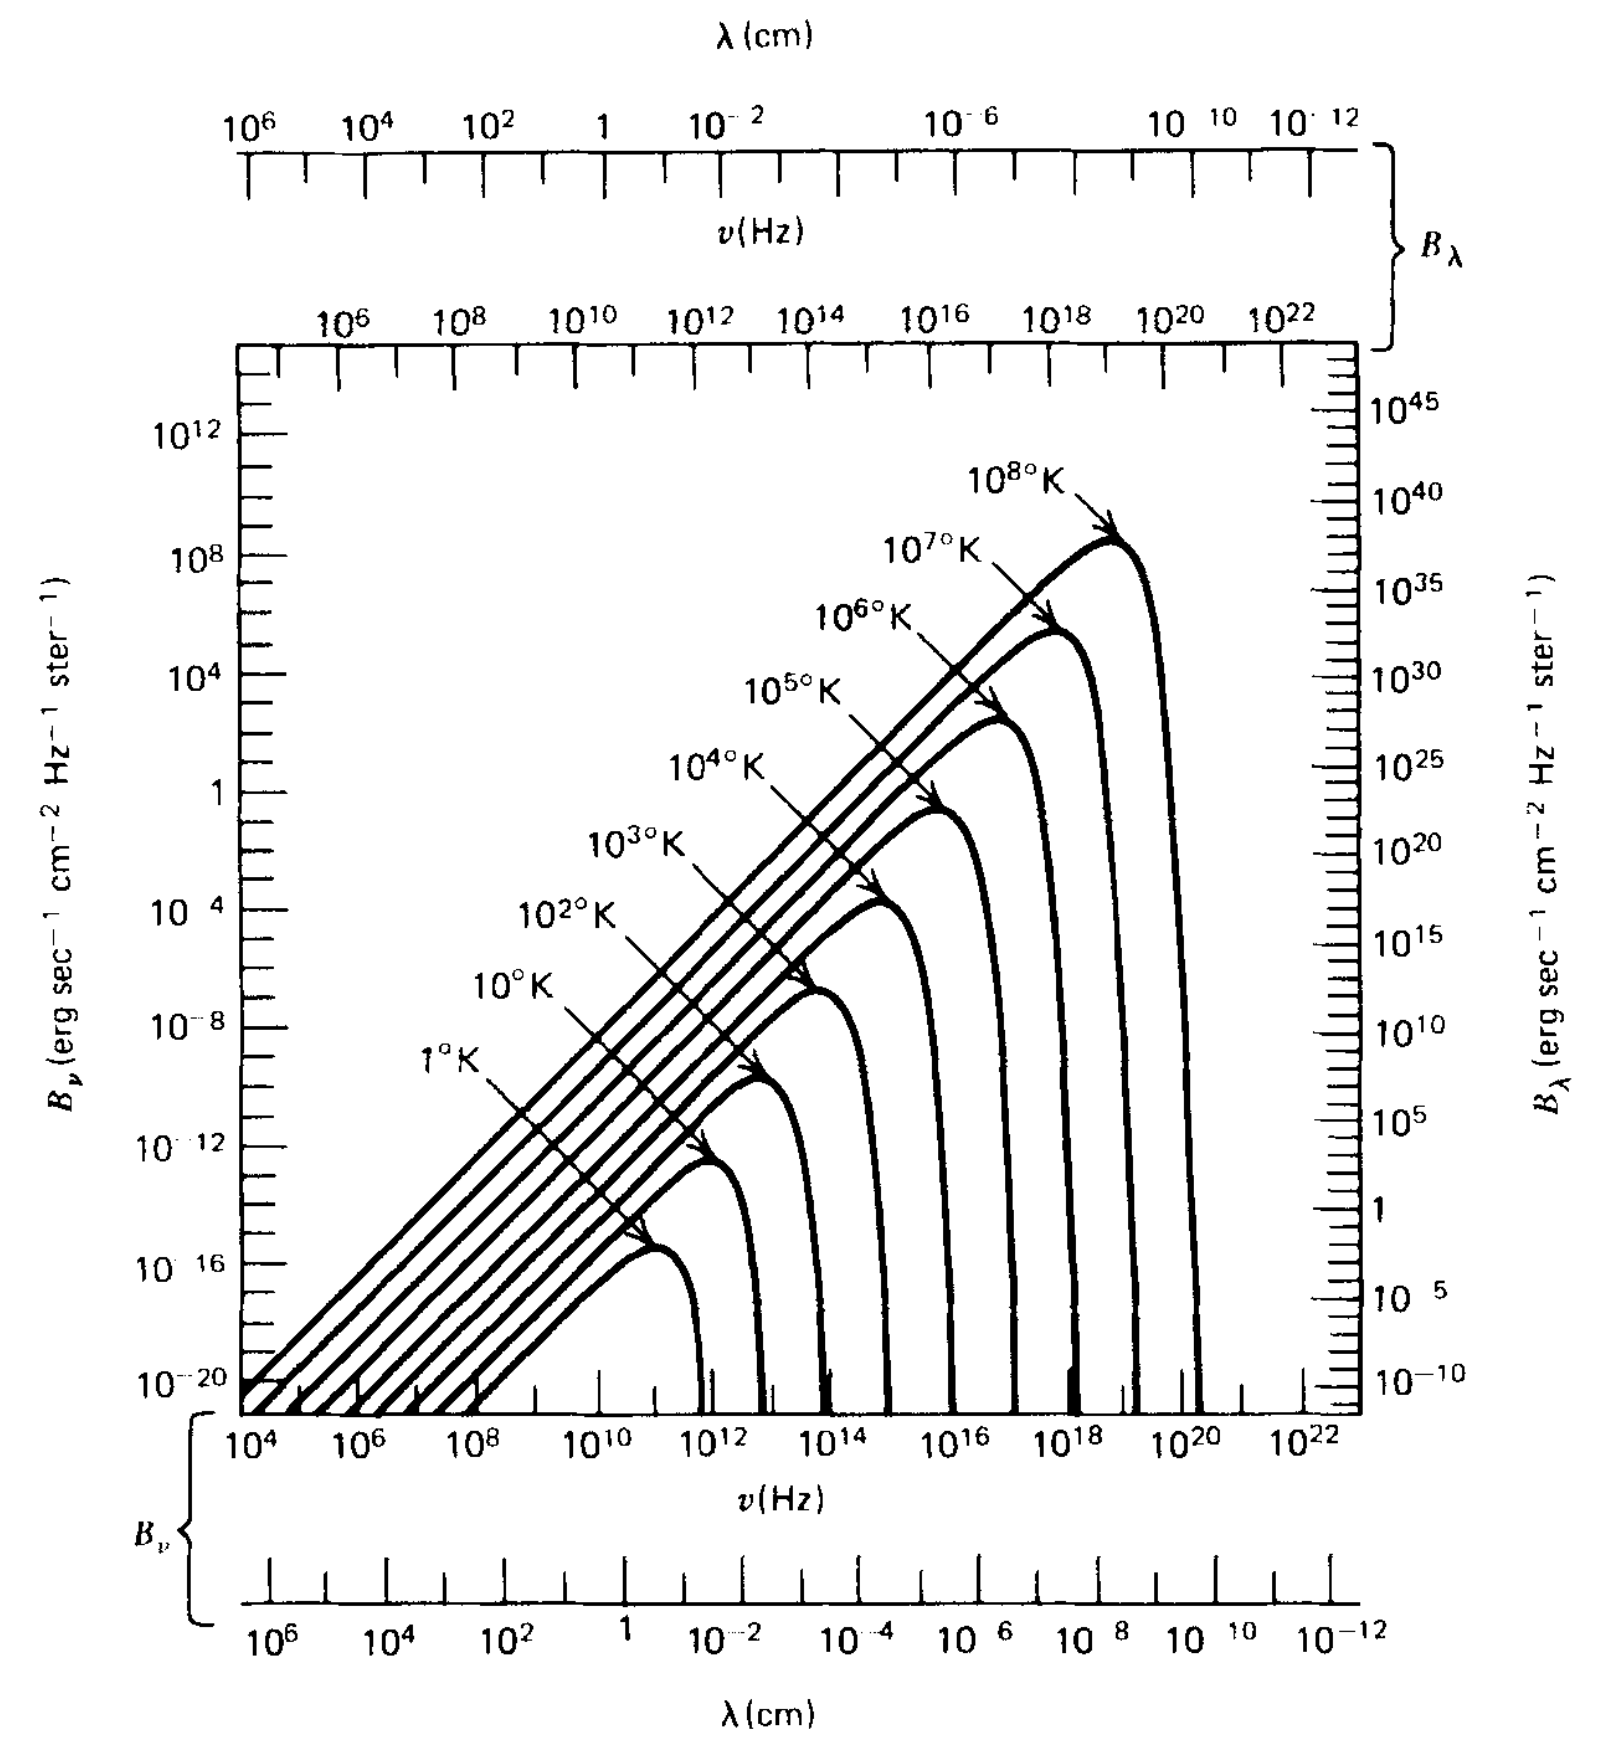
\includegraphics[width=12cm]{figures/cosmology/blackbody.png}
    \centering
    \caption{Blackbody spectra at various temperatures. Figure taken from Ryden (2017).}
    \label{fig:blackbody}
\end{figure}

{\noindent}Figure \ref{fig:blackbody} shows blackbody spectra for various temperatures in log-log space, where the peak of each blackbody spectrum is related to its associated temperature via $h\nu_\mathrm{peak} \approx 2.82\,k_BT$. While the mean photon energy is $2.82\,k_BT$, approximately one in ever 500 photons will have energies exceeding $10\,k_BT$, one in 3 million will exceed $20\,k_BT$, and one in 30 billion will exceed $30\,k_BT$. While only a small fraction of CMB photons are found in the high-energy tail-end of the Planck distribution, the overall number of CMB photons is enormous -- outnumbering baryons by nearly 2 billion to one. Therefore, the vast number of CMB photons surrounding neutral hydrogen atoms greatly increases the probability of photoionization, even with a mean photon energy less than the ionization energy of hydrogen.

\subsubsection{Follow-up Questions}

\begin{itemize}
    \item How is the CMB related to recombination?
    \item Around how long ago or at what redshift did this occur?
    \item What is the last scattering surface?
    \item Is the surface of last scattering a well-defined surface (i.e., did recombination happen suddenly)?
\end{itemize}

% --------------------------------------------------------------
%
%                           2. 
%
% --------------------------------------------------------------

\newpage
\subsection{Question 2}

The Universe is said to be ``flat," or, close to flat. What are the properties of a flat Universe and what evidence do we have for it?

\subsubsection{Short answer}

There are three simple properties of a flat Universe: (1) parallel lines never converge nor diverge; (2) the sum of all energy densities is equal to it's critical value; and (3) the sum of angles withing a triangle is always $180^\circ$. Two common techniques for measuring the curvature (i.e., topology) of the Universe include measuring the total energy density of the Universe ($\Omega_0$), and using the main peak in the CMB angular power spectrum ($C_\ell$) as a standard ruler for the size of the sound horizon at the surface of last scattering.

\subsubsection{Additional context}

In developing a mathematical theory of general relativity, in which spacetime geometry/curvature is related to the mass-energy density, Einstein needed a way of mathematically describing curvature. Since picturing the curvature of a four-dimensional spacetime is, to say the least, difficult, let's start by considering ways of describing the curvature of two-dimensional spaces, then extend what we have learned to higher dimensions.

{\noindent}The simplest of two-dimensional spaces is a plane, on which Euclidean geometry holds (see (a) of Figure \ref{fig:geometries}). On a plane, a geodesic is a straight line. If a triangle is constructed on a plane by connecting three points with geodesics, the sum of the angles made with its vertices obeys:

\begin{align*}
    \Delta_\mathrm{flat} = \alpha + \beta + \gamma = \pi ~~~~~[{\rm rad}].
\end{align*}

{\noindent}Note that a plane has infinite area, and has no upper limits on the possible distance between points.

{\noindent}Now consider another simple two-dimensional space, the surface of a sphere (see (b) of Figure \ref{fig:geometries}). On the surface of a sphere, a geodesic is a portion of a great circle -- that is, a circle whose center corresponds to the center of the sphere. If a triangle is constructed on the surface of the sphere by connecting three points with geodesics, the sum of the angles made with its vertices obeys:

\begin{align*}
    \Delta_\mathrm{closed} = \alpha + \beta + \gamma = \pi + A/R^2 ~~~~~[{\rm rad}],
\end{align*}

{\noindent}where $A$ is the area of the triangle, and $R$ is the radius of the sphere. All spaces in which $\alpha + \beta + \gamma > \pi$ are called ``positively curved'' spaces. The surface of a sphere is a positively curved two-dimensional space. Moreover, it is a space where the curvature is homogeneous and isotropic; no matter where you draw a triangle on the surface of a sphere, or how you orient it, it must always satisfy the above equation for $\Delta_\mathrm{closed}$. Note that a sphere has a maximum possible distance between points; the distance between antipodal points, at the maximum possible separation, is $\pi R$.

{\noindent}In addition to flat spaces and positively curved spaces, there exist negatively curved spaces. An example of a negatively curved two-dimensional space is the hyperboloid, or saddle-shape (see (c) of Figure \ref{fig:geometries}). If a triangle is constructed on this surface by connecting three points with geodesics, the sum of the angles made with its vertices obeys:

\begin{align*}
    \Delta_\mathrm{open} = \alpha + \beta + \gamma = \pi - A/R^2 ~~~~~[{\rm rad}],
\end{align*}

{\noindent}where $A$ is the area of the triangle, and $R$ is the radius of curvature. All spaces in which $\alpha + \beta + \gamma < \pi$ are called ``negatively curved'' spaces. The surface of a hyperboloid is a negatively curved two-dimensional space. A surface of constant negative curvature has infinite area, and has no upper limit on the possible distance between points.

\begin{figure}[h]
    \floatbox[{\capbeside\thisfloatsetup{capbesideposition={right,top},capbesidewidth=4cm}}]{figure}[\FBwidth]
    {\caption{\footnotesize{\\(a) Flat geometry for which $ \Delta_\mathrm{flat} = \alpha + \beta + \gamma = \pi$. (b) Closed geometry for which $\Delta_\mathrm{closed} = \alpha + \beta + \gamma = \pi + A/R^2$, where $A$ is the area of the triangle, and $R$ is the radius of the sphere. (c) Open geometry for which $\Delta_\mathrm{open} = \alpha + \beta + \gamma = \pi - A/R^2$, where $A$ is the area of the triangle, and $R$ is the radius of curvature.}}
    \label{fig:geometries}}
    {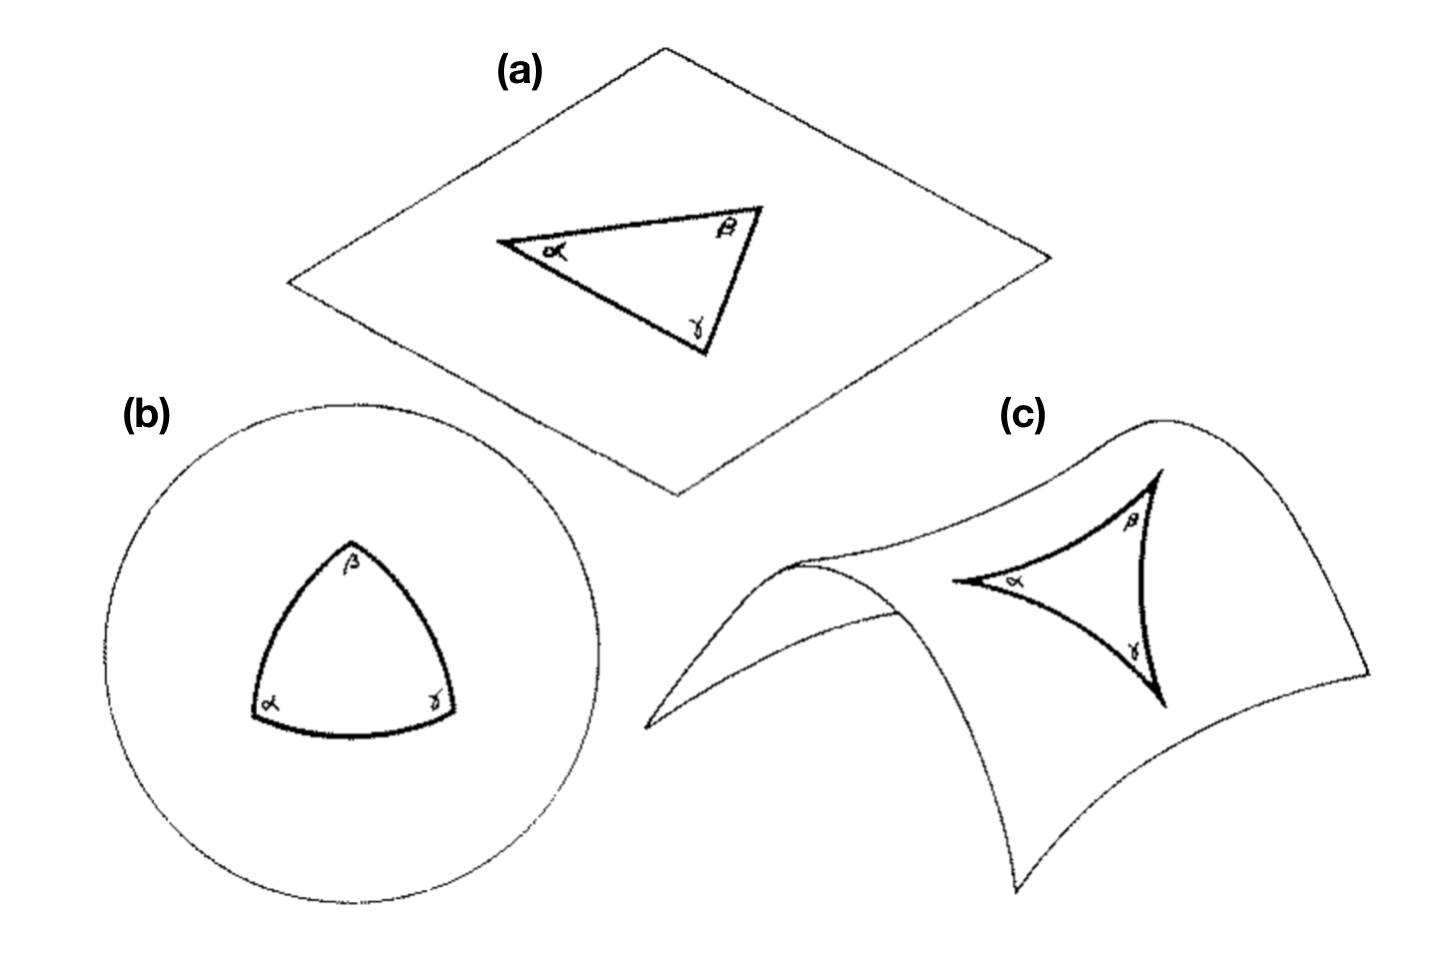
\includegraphics[width=10cm]{figures/cosmology/geometries.png}}
\end{figure}

{\noindent}If you want a two-dimensional space to be homogeneous and isotropic, there are only three possibilities that fit the bill: the space can be uniformly flat, it can have uniform positive curvature, or it can have uniform negative curvature. Thus, if a two-dimensional space has curvature which is homogeneous and isotropic, its geometry can be specified by two quantities, $\kappa$, and $R$. The number $\kappa$, called the curvature constant, is $\kappa = 0$ for a flat space, $\kappa = +1$ for a positively curved space, and $\kappa = −1$ for a negatively curved space. If the space is curved, then the quantity $R$, which has dimensions of length, is the radius of curvature.

{\noindent}The results for two-dimensional space can be extended straightforwardly to three dimensions. A three-dimensional space, if its curvature is homogeneous and isotropic, must be flat, have uniform positive curvature, or have uniform negative curvature. If a three-dimensional space is flat ($\kappa = 0$), it has the following metric:

\begin{align*}
    ds^2_\mathrm{flat} = dx^2 + dy^2 + dz^2.
\end{align*}

{\noindent}By making the simple coordinate substitution $x = r\cos\theta$, $y = r\sin\theta$, this can be written in spherical coordinates as:

\begin{align*}
    ds^2_\mathrm{flat} = dr^2 + r^2[d\theta^2 + \sin^2\theta d\phi^2].
\end{align*}

{\noindent}If a three-dimensional space has uniform positive curvature ($\kappa = +1$), its metric is

\begin{align*}
    ds_\mathrm{closed}^2 = dr^2 + R^2\sin^2(r/R)[d\theta^2 + \sin^2\theta d\phi^2].
\end{align*}

{\noindent}A positively curved three-dimensional space has finite volume, just as a positively curved two-dimensional space has finite area. The point at $r = \pi R$ is the antipodal point to the origin, just as the south pole, at $r = \pi R$, is the antipodal point to the north pole, at $r = 0$, on the surface of a sphere. By traveling a distance $C = 2\pi R$, it is possible to ``circumnavigate'' a space of uniform positive curvature.

{\noindent}If a three-dimensional space has uniform negative curvature ($\kappa =
−1$), its metric is

\begin{align*}
    ds_\mathrm{open}^2 = dr^2 + R^2\sinh^2(r/R)[d\theta^2 + \sin^2\theta d\phi^2].
\end{align*}

{\noindent}Like flat space, negatively curved space has infinite volume.

{\noindent}The three possible metrics for a homogeneous, isotropic, three-dimensional
space can be written more compactly in the form:

\begin{align*}
    ds^2 = dr^2 + S_\kappa(r)^2d\Omega^2
\end{align*}

{\noindent}where

\begin{align*}
    d\Omega \equiv d\theta^2 + \sin^2\theta d\phi^2
\end{align*}

{\noindent}and

\begin{equation*}
    S_\kappa(r) =
    \left\{
    \begin{aligned}
    R\sin(r/R), ~~~~~& (\kappa = +1) \\
              r,~~~~~& (\kappa = 0) \\
    R\sinh(r/R),~~~~~& (\kappa = -1)
    \end{aligned}
    \right.
    .
\end{equation*}

{\noindent}Here, $\kappa=0,-1,+1$ is the sign of curvature for a flat, open, and closed Universe, respectively. The coordinate system ($r,\theta,\phi$) is not the only possible system. For instance, if we switch the radial coordinate from $r$ to $x \equiv S_\kappa(r)$, the metric for a homogeneous, isotropic, three-dimensional space can be written in the form:

\begin{align*}
    ds^2 = \frac{dx^2}{1-\kappa x^2/R^2} + x^2d\Omega^2.
\end{align*}

{\noindent}\textbf{Energy density of the Universe}: The \textbf{critical density} of the Universe is defined to be

\begin{align*}
    \rho_c \equiv \left( \frac{3H_0^2}{8\pi G} \right) ~ [{\rm g\,cm^{-3}}]
\end{align*}

{\noindent}which allows the density parameter to be defined as

\begin{align*}
    \Omega_0 \equiv \frac{\rho}{\rho_c} ~ [{\rm dimensionless}].
\end{align*}

{\noindent}If the total energy density is greater than the critical density (i.e., $\Omega_0>1$), then the Universe is said to be \textbf{closed}: initially parallel lines eventually converge, just as lines of constant longitude meet at the North and South poles. A closed Universe, much like the surface of a sphere, has positive curvature. In a low-density Universe whose total energy density is less than critical value (i.e., $\Omega_0<1$), the Universe is said to be \textbf{open}: initially parallel lines eventually diverge, as would marbles rolling off a saddle. While a closed Universe has positive curvature, an open Universe has negative curvature. 

{\noindent}\textbf{CMB angular power spectrum}: The comparison between the predicted acoustic peak scale and its angular extent provides a measurement of the angular diameter distance to recombination. The angular diameter distance in turn depends on the spatial curvature and expansion history of the Universe. Assuming the size of the Universe's horizon at the time of recombination and the distance to the last scattering surface, the geometry (or curvature) of the Universe can be measured using the angular size of the first peak of the angular power spectrum. If the first peak is at $\ell\sim220$, the Universe is flat, whereas if the first peak is at $\ell<220$ or $\ell>220$, the Universe is open or closed, respectively.

% --------------------------------------------------------------
%
%                           3. 
%
% --------------------------------------------------------------

\newpage
\subsection{Question 3}

Outline the development of the Cold Dark Matter spectrum of density fluctuations from the early Universe to the current epoch.

\subsubsection{Short answer}

The primordial CDM spectrum is that of the scale-invariant \textbf{Harrison-Zeldovich power spectrum} (i.e., a flat power spectrum favouring neither large nor small scales). As the sound horizon grows, continuously larger modes are encompassed and become in causal contact which allows them to begin collapsing under their own self-gravity. The CDM power spectrum therefore begins to diverge from a flat spectrum at small modes which continues until the Universe turns over from being radiation-dominated to matter-dominated. At this point, the CDM power spectrum is frozen-in and there is a characteristic peak at $\sim250\,{\rm Mpc}$ which is defined by the sound horizon.

\subsubsection{Additional context}

The generally accepted theoretical framework for the formation of structure is that of gravitational instability. The gravitational instability scenario assumes that the early Universe was almost perfectly smooth, with the exception of tiny density perturbations with respect to the global cosmic background density and the accompanying tiny velocity perturbations from the general Hubble expansion. The observed fluctuations in the CMB temperature are a reflection of these density perturbations, so we know that the primordial density perturbations must have been on the order of $\Delta T / T \sim 10^{-5}$. The origin of this density perturbation field has yet to be fully understood, but the most plausible theory currently is that they are a result of \textbf{quantum fluctuations} which, during the inflationary phase, expanded to macroscopic scales.

{\noindent}Originally minute deviations from the average density of the Universe, and the corresponding deviations from the global cosmic expansion velocity (i.e., the \textbf{Hubble expansion}), will start to grow under the influence of gravity where the density perturbations will have induced local differences in gravity. During its early evolution, an overdensity will experience a gradually stronger deceleration of its expansion velocity such that its expansion velocity will continue to slow down with respect to the Hubble expansion. Since matter is gravitationally attracted to regions of higher density, it will also have the tendency to move towards that region. When the region has become sufficiently overdense, the mass of the density perturbation will have grown so much that its expansion would come to a halt. The region then completely decouples from the Hubble expansion and begins to collapse under its own gravity. The newly formed gravitationally bound object will reach virial equilibrium at which point it becomes a recognizable comic object; its precise nature (e.g., galaxy, cluster of galaxies etc.) being determined by the properties of the initial density perturbation and its surroundings.

{\noindent}The opposite tendency will have occurred for underdensities in the matter density field. Since they contain less matter than the average density field, its expansion deceleration is less than the Hubble expansion which results in matter becoming even more dispersed and underdensities continuing to expand. As this process continues and becomes more pronounced, such underdensities result in the gradual emergence of voids in the matter distribution of the Universe. The most dramatic evidence for these spatial nonuniformities (i.e., overdensities and voids) on the largest of scales comes from redshift surveys such as the 2dF Galactic Redshift Survey\footnote{\href{http://www.2dfgrs.net/}{2dFGRS: http://www.2dfgrs.net/}} shown in Figure \ref{fig:2df}.

\begin{figure}[h]
    \floatbox[{\capbeside\thisfloatsetup{capbesideposition={right,top},capbesidewidth=4cm}}]{figure}[\FBwidth]
    {\caption{\footnotesize{The spatial distribution of galaxies in two four-degree strips on the sky, according to the 2dF Galaxy Redshift Survey. Note the $100\,{\rm Mpc}$ filamentary features and the prominent voids. One of the principal challenges in cosmology is to explain this pattern, which is most probably a relic of the very earliest stages of the expanding Universe. Figure taken from Ryden (2017).}}
    \label{fig:2df}}
    {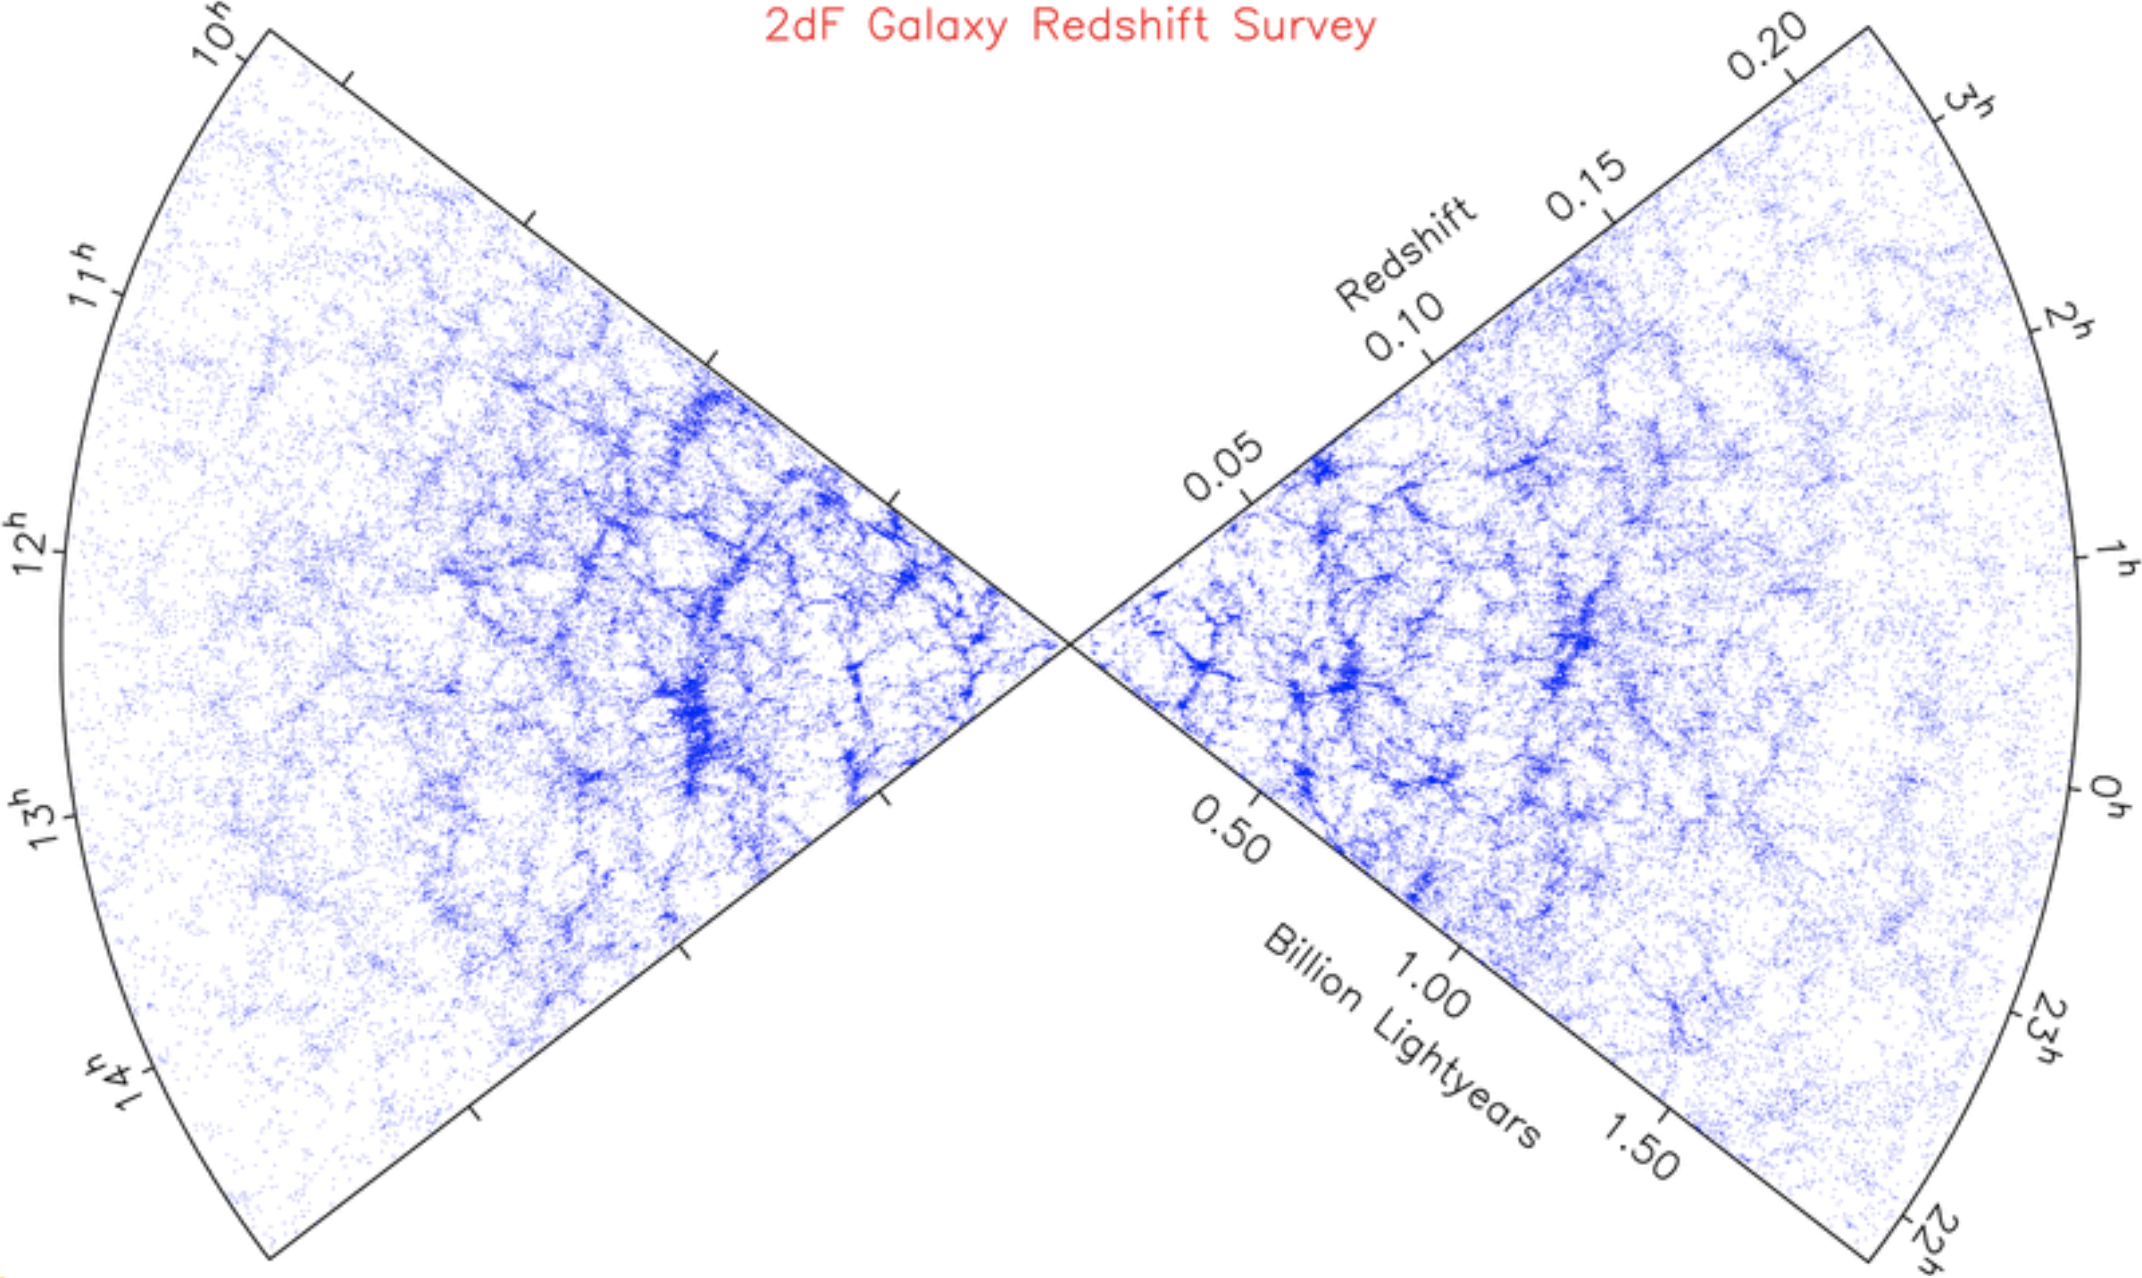
\includegraphics[width=10cm]{figures/cosmology/2df.png}}
\end{figure}

{\noindent}Galaxies in Figure \ref{fig:2df} are clearly not distributed randomly: the Universe has structure on large scales. To understand this structure, we must go beyond the Standard Model not only by including dark matter, but also by allowing for deviations from smoothness. We must develop the tools to study perturbations around the smooth background of the Standard Model. This is straightforward in theory, as long as the perturbations remain small (i.e., linear). Indeed, understanding the development of structure in the Universe has become a major goal of most cosmologists today. Dark matter is needed not only to explain rotation curves of galaxies but to explain structure in the Universe at large!

{\noindent}The best ways to learn about the evolution of structure and to compare theory with observations are to look at anisotropies in the CMB and at how matter is distributed on large scales. Anisotropies in the CMB today tell us what the Universe looked like when it was several hundred thousand years old, so they are wonderful probes of the perturbations. To compare theory with observations, we must at first try to avoid scales dominated by nonlinearities. As an extreme example, we can never hope to understand cosmology by carefully examining rock formations on Earth. The intermediate steps -- collapse of matter into a galaxy; molecular cooling; star formation; planetary formation; etc. -- are much too complicated to allow comparison between linear theory and observations. While perturbations to matter on small scales (less than about $100\,{\rm Mpc}$) have grown nonlinear, large-scale perturbations are still small so they have been processed much less than the corresponding small-scale structure. Similarly, anisotropies in the CMB have remained small because the photons that make up the CMB do not clump.

{\noindent}Identifying large-scale structure and the CMB as the two most promising areas of study solves just one issue. Another very important challenge is to understand how to characterize these distributions so that theory can be compared to experiment. It is one thing to look at a map and quite another to quantitatively test cosmological models. To make such tests, it is often useful to take the Fourier transform of the distribution in question; as we will see, working in Fourier space makes it easier to separate large from small scales. The most important statistic in the cases of both the CMB and large-scale structure is the \textbf{two-point correlation function}, called the \textbf{power spectrum} in Fourier space.

\begin{figure}[t]
    \floatbox[{\capbeside\thisfloatsetup{capbesideposition={right,top},capbesidewidth=4cm}}]{figure}[\FBwidth]
    {\caption{\footnotesize{The variance $\Delta^2 \equiv k^3P(k)/2\pi^2$ of the Fourier transform of the galaxy distribution as a function of scale. On large scales, the variance is smaller than unity so the distribution is smooth. The solid line is the theoretical model in which the Universe contains dark matter and a cosmological constant with perturbations generated by inflation. The dashed line is a model with only baryons and no dark matter. Data came from the PSCz survey (Saunders et al, 2000) as analyzed by Hamilton and Tegmark (2001). Figure from Ryden (2017).}}
    \label{fig:galaxypowerspec}}
    {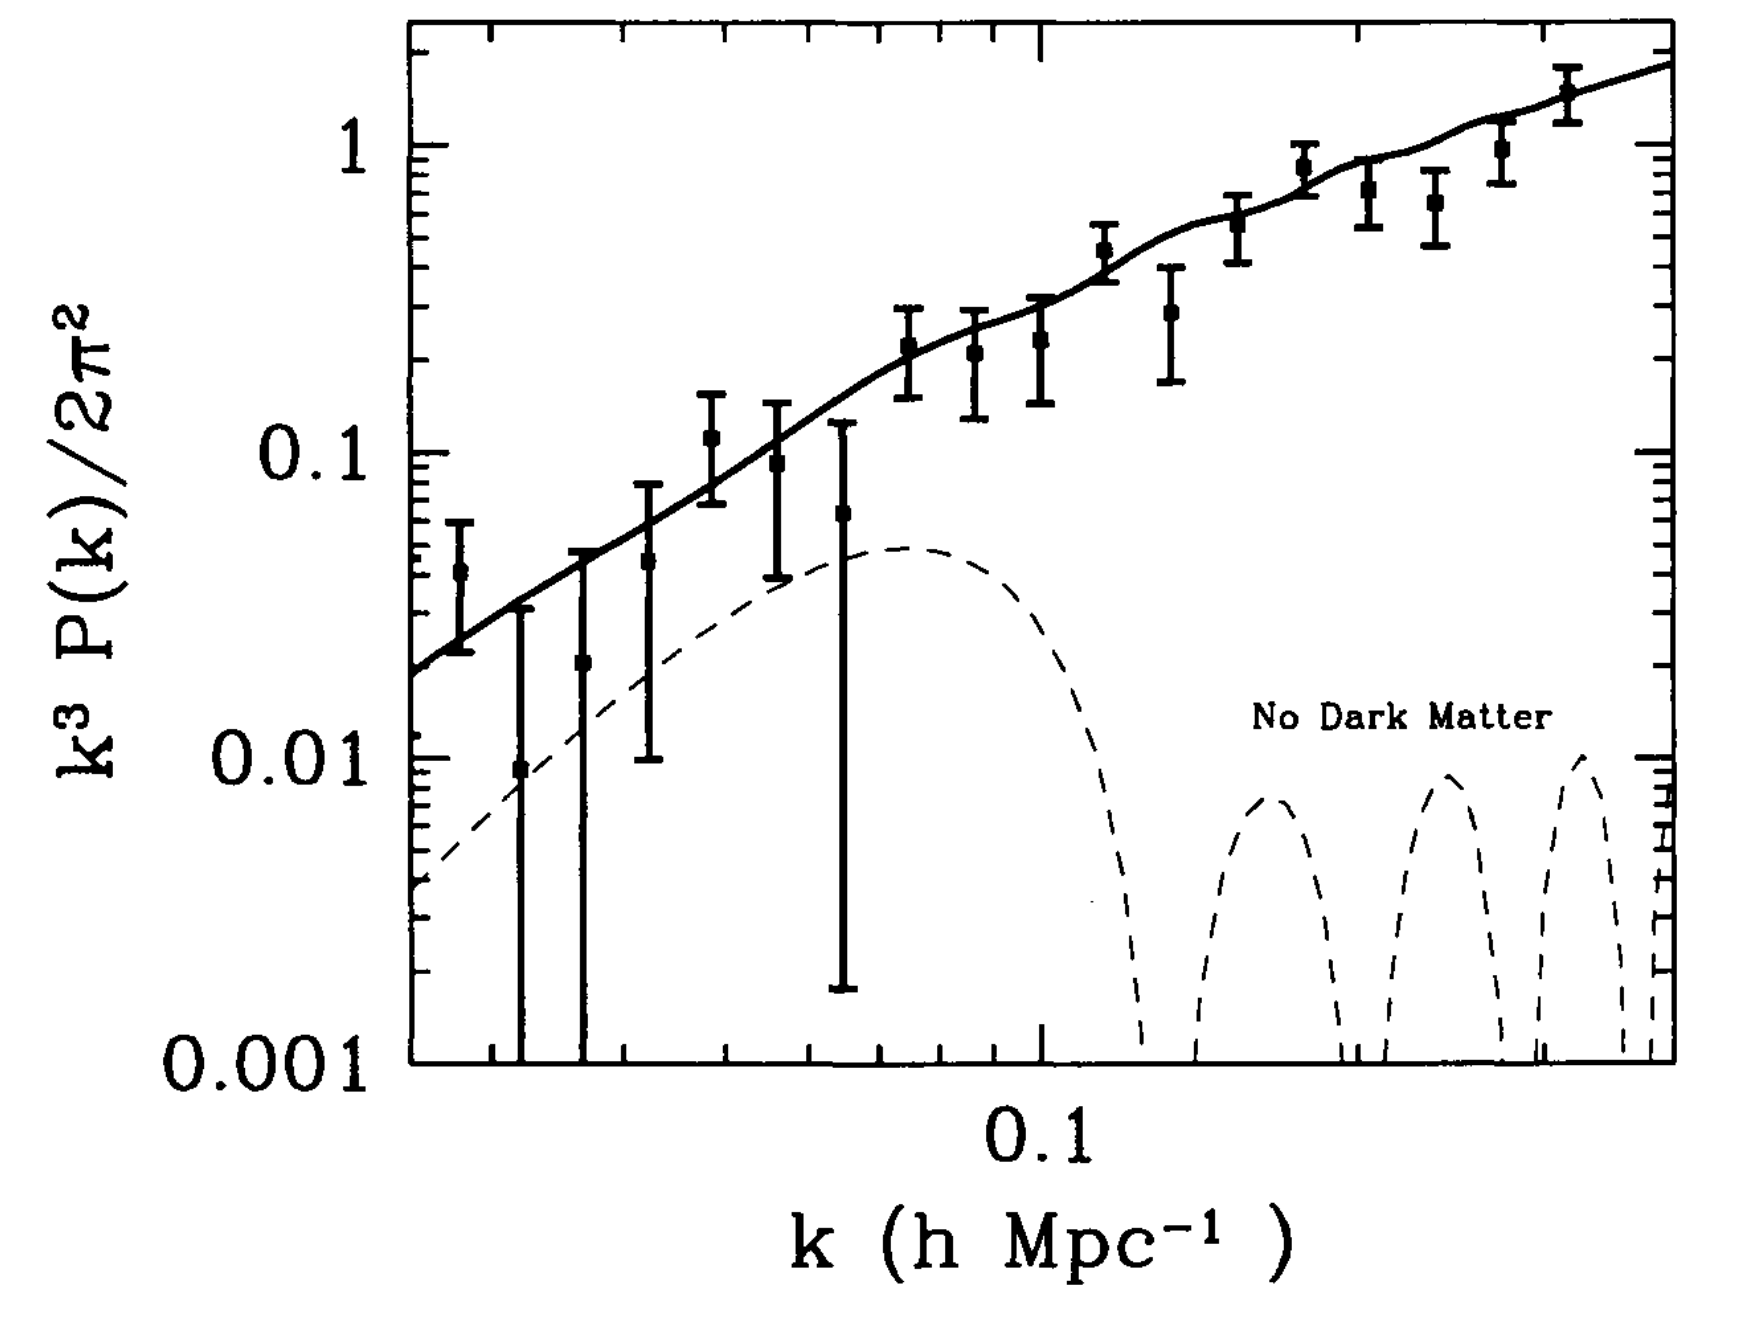
\includegraphics[width=9cm]{figures/cosmology/GalaxyPowerSpectrum.png}}
\end{figure}

{\noindent}If the mean density of galaxies at some time $t$ is $\langle\rho(t)\rangle$, then we can characterize the inhomogeneities with the dimensionless \textbf{density perturbation field} (also known as the \textbf{density contrast}) which is used to relate the energy density $\rho(\mathbf{x},t)$ at some co-moving spatial coordinate $\mathbf{x}$ and time $t$ to the average energy density at that time $\langle\rho(t)\rangle$:

\begin{align*}
    \delta(\mathbf{x},t) \equiv \frac{\rho(\mathbf{x},t)~- \langle\rho(t)\rangle}{\langle\rho(t)\rangle} ~ [{\rm dimensionless}].
\end{align*}

{\noindent}Evidently, in an unperturbed Universe with $\rho(\mathbf{x},t) = \langle\rho(t)\rangle$ everywhere, $\delta(\mathbf{x},t) = 0$. Note that positive density fluctuations (i.e., overdensities) may in principle grow limitless whereas negative density fluctuations (i.e., underdensities) have a strict lower-limit of $\delta \geq -1$ (emptier than empty simply doesn't exist). In a complete description of density perturbations, the total energy density of the Universe includes components of baryonic matter ($\rho_b$), cold dark matter ($\rho_c$), radiation ($\rho_\mathrm{rad}$), and dark energy ($\rho_\Lambda$):

\begin{align*}
    \rho(\mathbf{x},t) = \rho_b(\mathbf{x},t) + \rho_c(\mathbf{x},t) + \rho_\mathrm{rad}(\mathbf{x},t) + \rho_\Lambda(\mathbf{x},t) ~ [{\rm g\,cm^{-3}}].
\end{align*}

{\noindent}In terms of their global gravitational influence, dark matter and baryonic matter contribute and evolve equivalently, therefore on cosmological scales they can be combined into a total matter energy density $\rho_m = \rho_b + \rho_c$. Each component may have its own (primordial) perturbation character. Dark energy does not have any density fluctuations, so $\delta_\Lambda(\mathbf{x},t) = 0$. Since most of the structure formation happened during the \textit{matter-dominated era}, this mainly involves the evolution of matter linear perturbations $\delta_m(\mathbf{x},t)$.

{\noindent}In addition to the density contrast, an alternative (and equivalent) description of the statistical properties of the matter distribution in the Universe is the \textbf{power spectrum} $P(k)$. Roughly speaking, the power spectrum describes the level of structure as a function of the length scale $L \simeq 2\pi/k$ where $k$ is a co-moving wavenumber. Phrased differently, the density fluctuations are decomposed into a set of plane waves of the form $\delta(\mathbf{x}) = \sum a_k\cos(\mathbf{x\cdot k})$ with wave vector $\mathbf{k}$ and amplitude $a_k$. The power spectrum $P(k)$ then describes the mean of the squares of the amplitudes $\lvert a_k \rvert^2$ averaged over all wave vectors with equal length $\lvert\mathbf{k}\rvert = k$. Technically speaking, this is a Fourier decomposition. The Fourier transform of $\delta(\mathbf{x},t)$ is $\tilde{\delta}(\mathbf{x},t)$, which allows the power spectrum $P(k)$ to be defined via

\begin{align*}
    \langle \tilde{\delta}(\mathbf{k}) \tilde{\delta}(\mathbf{k'}) \rangle = (2\pi)^3 P(k) \delta^3 (\mathbf{k} - \mathbf{k'}) ~ [{\rm \mu K^2}],
\end{align*}

{\noindent}where the angular brackets denote averaging over the entire distribution, $k$ is the wavenumber, and $\delta^3()$ is the delta Dirac function which constrains $\mathbf{k}=\mathbf{k'}$. This indicates that the power spectrum is the spread, or the variance, in the distribution. Figure \ref{fig:galaxypowerspec} shows the combination $k^3P(k)/2\pi^2$, a dimensionless number which is a good indication of the clumpiness on scale $k$.

{\noindent}The power spectrum $P(k)$ and the two-point correlation function $\xi(x)$ are related through the Fourier transform as

\begin{align*}
    P(k) = 2\pi \int\limits_0^\infty \frac{\sin(kx)}{kx} x^2 \xi(x)\,{\rm d}x ~ [{\rm \mu K^2}],
\end{align*}

{\noindent}i.e., the integral over the correlation function with a weight factor depending on the wave number provides the power spectrum. This relation can also be inverted to obtain the inverse Fourier transform such that the correlation function can be computed from the power spectrum. In general, knowing the power spectrum is insufficient to unambiguously describe the statistical properties of any density field; as such, the power spectrum is often used alongside the correlation function $\xi(x)$. Given observation data, either the power spectrum or the correlation function may be easier to compute, or another may be easier to obtain from models or simulations. In addition, our intuitive understanding of these functions may vary in different situations.

\begin{figure}[t]
    \floatbox[{\capbeside\thisfloatsetup{capbesideposition={right,top},capbesidewidth=4cm}}]{figure}[\FBwidth]
    {\caption{\footnotesize{Anisotropies in the CMB predicted by the theory of inflation compared with observations, x-axis is multipole moment (e.g., $\ell = 1$ is the dipole, $\ell = 2$ the quadrupole) so that large angular scales correspond to low $\ell$; y-axis is the root mean square anisotropy (the square root of the two-point correlation function) as a function of scale. The characteristic signature of inflation is the series of peaks and troughs, a signature which has been verified by experiment. Figure from Ryden (2017).}}
    \label{fig:cmbpowerspec}}
    {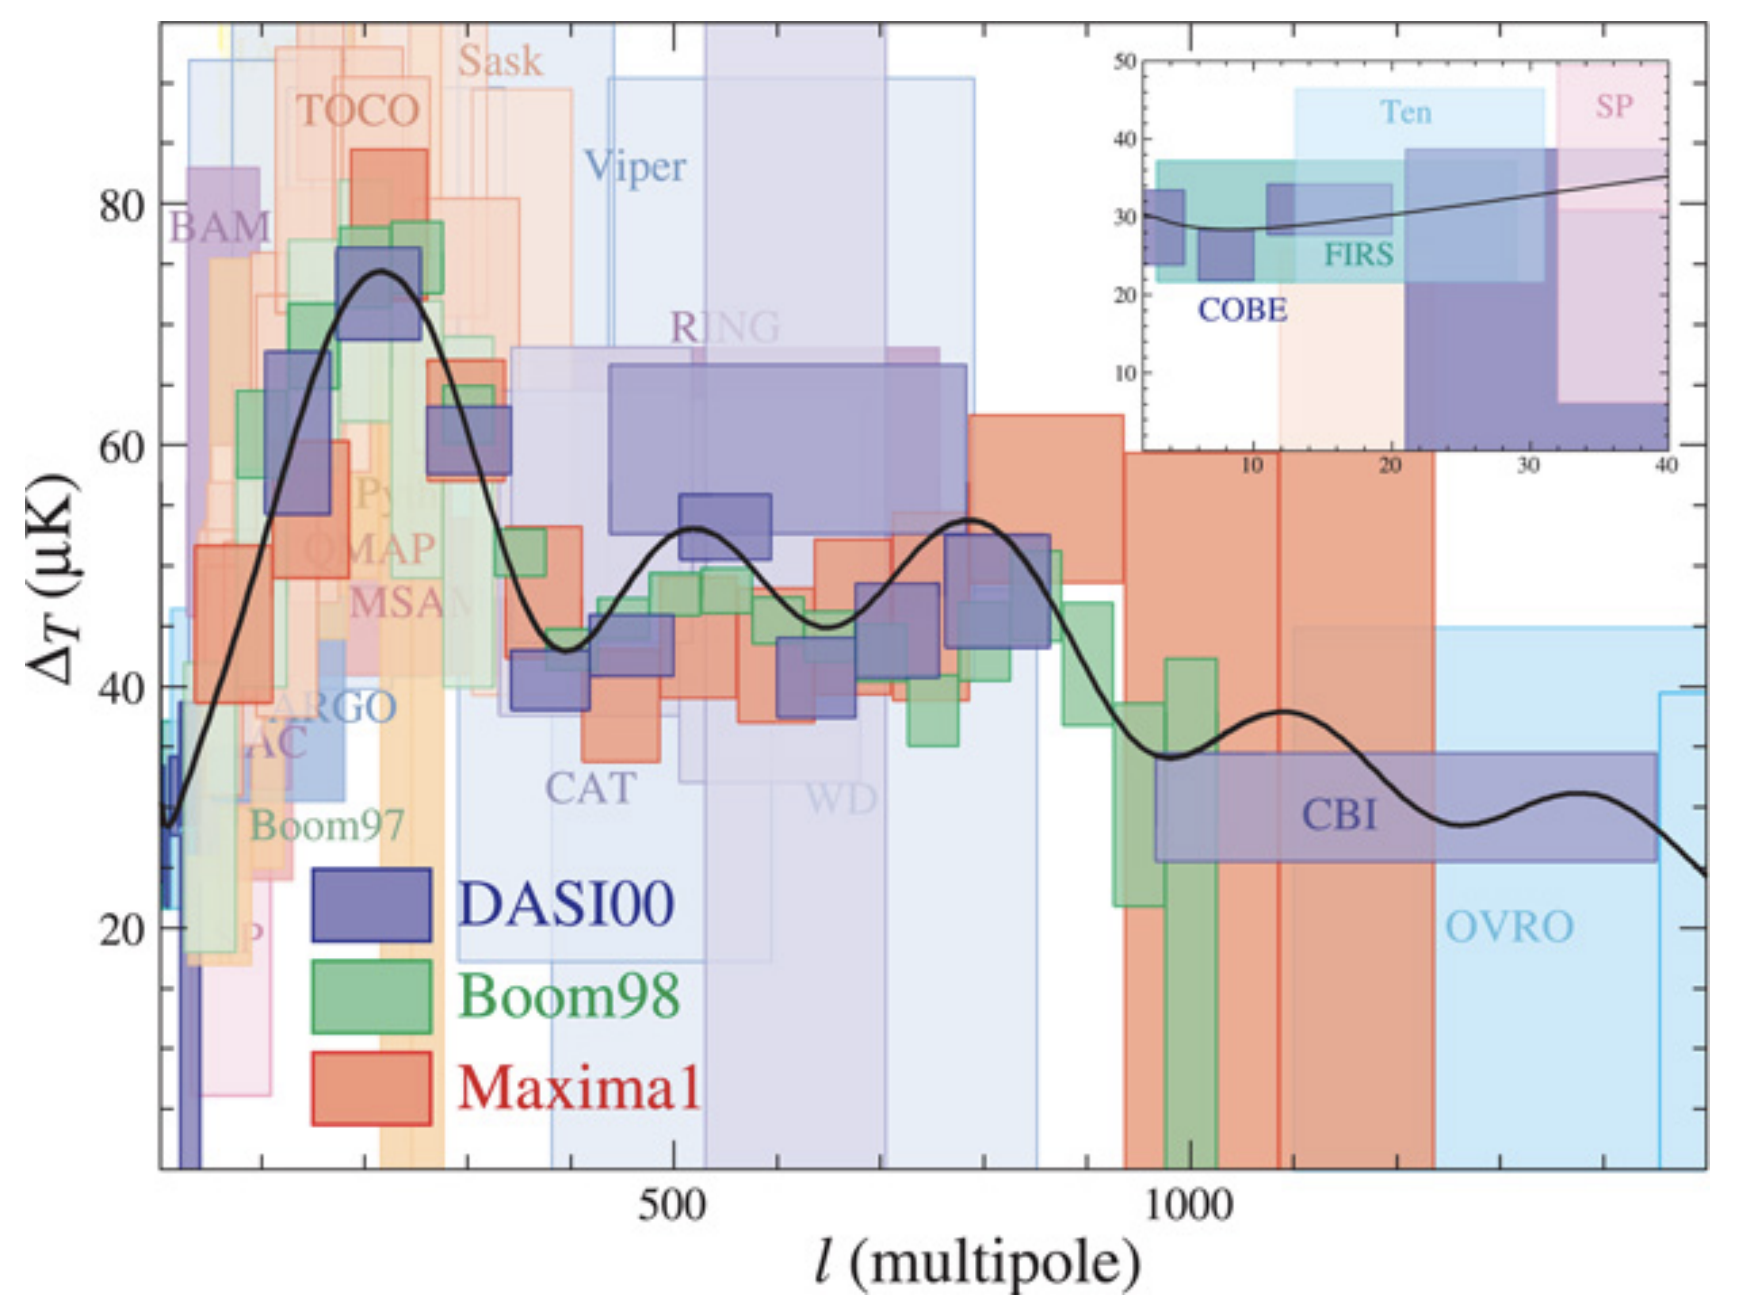
\includegraphics[width=12cm]{figures/cosmology/CMBPowerSpectrum.png}}
\end{figure}

{\noindent}The best measure of anisotropies in the CMB is also the two-point correlation function of the temperature distribution. There is a subtle technical difference between the two power spectra which are used to measure the galaxy distribution and the CMB, though. The difference arises because the CMB temperature is a two-dimensional field, measured everywhere on the sky (i.e., with two angular coordinates). Instead of Fourier transforming the CMB temperature, then, one typically expands it in spherical harmonics, a basis more appropriate for a 2D field on the surface of a sphere. Therefore the two-point correlation function of the CMB is a function of multipole moment $\ell$, not wave number $k$. Figure \ref{fig:cmbpowerspec} shows the measurements of dozens of groups since 1992, when COBE first discovered large-angle (low $\ell$ in the plot) anisotropies.

{\noindent}It is assumed that in very early epochs, the matter density field obeyed Gaussian statistics. This is a prediction of a large class of inflationary models which are supposed to generate the primordial density fluctuations of the Universe. An important property of Gaussian statistics, or \textit{Gaussian random fields}, is that their distributions are uniquely determined by their power spectrum $P(k)$. Among the properties which characterize these Gaussian random fields, the probability distribution of the density fluctuations $\delta(\mathbf{x})$ at any point is a Gaussian distribution. Observational evidence for the Gaussian nature of the early density fluctuations comes from observations of anisotropies in the CMB which very strongly constrain any possible deviation from a Gaussian random field in the early Universe.

{\noindent}The early linear stages of structure formation have been successfully and completely worked out within the context of \textit{linear perturbation theory}. For this discussion of the growth of density perturbations, we are concentrating on length scales that are substantially smaller than the Hubble radius. On such scales, structure growth can be described in the framework of the Newtonian theory of gravity; the effects of spacetime curvature and thus General Relativity need only be accounted for when density perturbations are on length scales comparable to, or larger than, the Hubble radius. In addition, we assume for simplicity that the matter in the Universe consists of only pressure-free matter described in the \textit{fluid approximation}.

{\noindent}Approximate solutions of the set of equations which describe small deviations from the homogeneous solution have the form

\begin{align*}
    \delta(\mathbf{x},t)=D(t)\tilde{\delta}(\mathbf{x}) ~ [{\rm dimensionless}],
\end{align*}

{\noindent}i.e., the spatial and temporal dependencies factorize in these solutions. Here, $\tilde{\delta}(\mathbf{x})$ is an arbitrary function of the spatial coordinate, and D(t) satisfies the equation

\begin{align*}
    \ddot{D}(t)+\frac{2\dot{a}}{a}\dot{D}(t)-4\pi G\bar{\rho}(t)D(t) = 0 ~ [{\rm dimensionless}].
\end{align*}

{\noindent}The differential equation has two linearly independent solutions. One can show that one of them increases with time, whereas the other decreases. If, at some early time, both functional dependencies were present, the increasing solution will dominate at later times, whereas the solution decreasing with $t$ will become irrelevant. Therefore, we will consider only the increasing solution, which is denoted by $D_+(t)$, and normalize it such that $D_+(t_0)=1$. Then, the density contrast becomes

\begin{align*}
    \delta(\mathbf{x},t) = D_+(t)\delta_0(\mathbf{x}) ~ [{\rm dimensionless}].
\end{align*}

{\noindent}This mathematical consideration allows us to draw immediately a number of conclusions. First, the solution implies that in linear perturbation theory the spatial shape of the density fluctuations is frozen in comoving coordinates, only their amplitude increases. The growth factor $D_+(t)$ of the amplitude follows a simple differential equation that is readily solvable for any cosmological model. In fact, one can show that for arbitrary values of the density parameters in matter and vacuum energy, the growth factor has the form

\begin{align*}
    D_+(t) \propto \frac{H(a)}{H_0}\int\limits_0^a \frac{da'}{[\Omega_m/a'+\Omega_\Lambda a'^2-(\Omega_m+\Omega_\Lambda-1)]^{3/2}},
\end{align*}

{\noindent}where the factor of proportionality is determined from the condition $D_+(t_0)=1$.

{\noindent}Primordial density perturbations on a small scale appear to have a much higher amplitude than those on larger scales. This leads to a hierarchical process of structure formation, with small-scale perturbations being the first one to become nonlinear and develop into cosmic objects.

{\noindent}Returning to the two-point correlation function and Fourier transform, $P(k)$ and $\xi(x)$ both depend on cosmological time or redshift because the density field in the Universe evolves over time. Therefore, the dependence on $t$ is explicitly written as $P(k,t)$ and $\xi(x,t)$. Note that $P(k,t)$ is linearly related to $\xi(x,t)$ and $\xi(x,t)$ in turn depends quadratically on the density contrast $\delta$. If $x$ is the comoving separation vector, we then know the time dependence of the density fluctuations, $\delta(x,t)=D_+(t)\delta_0(\mathbf{x})$. Thus,

\begin{align*}
    \xi(x,t) = D_+^2(t)\xi(x,t_0),
\end{align*}

{\noindent}and accordingly,

\begin{align*}
    P(k,t) = D_+^2(t)P(k,t_0) \equiv D_+^2(t)P_0(k)  ~ [{\rm \mu K^2}],
\end{align*}

{\noindent}We stress that these relations are valid only in the framework of Newtonian, linear perturbation theory in the matter dominated era of the Universe. This last equation states that the knowledge of $P_0(k)$ is sufficient to obtain the power spectrum $P(k,t)$ at any time, again within the framework of linear perturbation theory.

{\noindent}Initially it may seem as if $P_0(k)$ is a function that can be chosen arbitrarily, but one objective of cosmology is to calculate this power spectrum and to compare it to observations. More than 30 years ago, arguments were already developed to specify the functional form of the initial power spectrum.

{\noindent}At early times, the expansion of the Universe follows a power law, $a(t)\propto t^{1/2}$ in the radiation-dominated era. At that time, no natural length-scale existed in the Universe to which one might compare a wavelength. The only mathematical function that depends on a length but does not contain any characteristic scale is a power law; hence for very early times one should expect

\begin{align*}
    P(k) \propto k^{n_s}  ~ [{\rm \mu K^2}].
\end{align*}

{\noindent}Many years ago, Harrison, Zeldovich, Peebles and others argued that $n_s=1$, as for this slope, the amplitude of the fluctuations of the gravitational potential are constant (i.e., preferring neither small nor large scales). For this reason, this spectrum with $n_s=1$ is called a scale-invariant spectrum, or Harrison-Zeldovich spectrum. With such a spectrum, we may choose a time $t_i$ after the inflationary epoch and write

\begin{align*}
    P(k,t_i) = D_+^2(t_i)Ak^{n_s} ~ [{\rm \mu K^2}],
\end{align*}

{\noindent}where $A$ is a normalization constant that cannot be determined from theory but has to be fixed by observations. However, this is not the complete story: the result needs to be modified to account for the different growth of the amplitude of density fluctuations in the radiation-dominated epoch of the Universe, compared to that in the later cosmic epochs from which our result was derived.

{\noindent}Furthermore, these modifications depend on the nature of the dark matter. One distinguishes between cold dark matter (CDM) and hot dark matter (HDM). These two kinds of dark matter differ in the characteristic velocities of their constituents. Cold dark matter has a velocity dispersion that is negligible compared to astrophysically relevant velocities (e.g., the virial velocities of low-mass dark matter halos). Therefore, their initial velocity dispersion can well be approximated by zero, and all dark matter particles have the bulk velocity of the cosmic `fluid' (before the occurrence of multiple streams). In contrast, the velocity dispersion of hot dark matter is appreciable; neutrinos are the best candidates for HDM, in view of their known abundance, determined from the thermal history of the Universe, and their finite rest mass. The characteristic velocity of neutrinos is fully specified by their rest mass; despite their low temperature of $T_\nu=1.9\,{\rm K}$ today, their thermal velocities of

\begin{align*}
    v_\nu \sim 150(1+z)\left(\frac{m_\nu}{1\,{\rm eV}}\right)^{-1} ~ [{\rm km\,s^{-1}}]
\end{align*}

{\noindent}prevent them from forming matter concentrations at all mass scales except for the most massive ones, as their velocity is larger than the corresponding escape velocities. In other words, the finite velocity dispersion of HDM is equivalent to assigning to it a pressure, which prevents them to fall into shallow gravitational potential wells. We will see below the dramatic differences between these two kinds of dark matter for the formation of structures in the Universe. In particular, this estimate shows that neutrinos cannot account for the dark matter on galaxy scales, and thus cannot explain the flat rotation curves of spiral galaxies.

{\noindent}If density fluctuations become too large on a certain scale, linear perturbation theory breaks down and the linear approximation to the solution of $P(k,t)$ is no longer valid. Then the true current-day power spectrum $P(k,t_0)$ will deviate from $P_0(t)$. Nevertheless, in this case it is still useful to examine $P_0(t)$ -- it is then called the linearly extrapolated power spectrum.

{\noindent}Within the framework of linear Newtonian perturbation theory in the `cosmic fluid', $\delta(\mathbf{x},t) = D_+(t)\delta(\mathbf{x})$ applies. Modifications to this behavior are necessary for several reasons:

\begin{itemize}
    \item If dark matter consists (partly) of HDM, this may not be gravitationally bound to the potential well of a density concentration. In this case, the particles are able to move freely and to escape from the potential well, which in the end leads to its dissolution if these particles dominate the matter overdensity. From this argument, it follows immediately that for HDM, small-scale density perturbations cannot form. For CDM this effect of free streaming does not occur.
    \item At redshifts $z\gtrsim z_\mathrm{eq}$, radiation dominates the density of the Universe. Since the expansion law $a(t)$ is then distinctly different from that in the matter-dominated phase, the growth rate for density fluctuations will also change.
    \item A cosmic horizon exists with comoving scale $r_\mathrm{H,com}(t)$. Physical interactions can take place only on scales smaller than $r_\mathrm{H,com}(t)$. For fluctuations of length-scales $L\sim2\pi/k\gtrsim r_\mathrm{H,com}(t)$, Newtonian perturbation theory will cease to be valid, and one needs to apply linear perturbation theory in the framework of the General Relativity.
\end{itemize}

{\noindent}These effects together will lead to a modification of the shape of the power spectrum, relative to the relation $P(k,t_i)=D_+^2(t_i)Ak^{n_s}$; for example, the evolution of perturbations in the radiation-dominated cosmos proceeds differently from that in the matter-dominated era. The power spectrum $P(k)$ is affected by the combination of the above effects, and will be different from the primordial spectral shape, $P\propto k^{n_s}$. The modification of the power spectrum is described in terms of the transfer function $T(k)$ in the form

\begin{align*}
    P(k,t) = D_+^2(t) Ak^{n_s}T^2(k)  ~ [{\rm \mu K^2}].
\end{align*}

{\noindent}The transfer function can be computed for any cosmological model if the matter content of the Universe is specified. In particular, $T(k)$ depends on the nature of dark matter.

{\noindent}The first of the above points immediately implies that a clear difference must exist between HDM and CDM models regarding structure formation and evolution. In HDM models, small-scale fluctuations are washed out by free-streaming of relativistic particles (i.e., the power spectrum is completely suppressed for large $k$, which is expressed by the transfer function $T(k)$ decreasing exponentially for large $k$). In the context of such a theory, very large structures will form first, and galaxies can form only later by fragmentation of large structures. However, this formation scenario is in clear contradiction with observations. For example, we observe galaxies and QSOs at $z>6$ so that small-scale structure is already present at times when the Universe had less than 10\% of its current age. In addition, the observed correlation function of galaxies, both in the local Universe (see Figure \ref{fig:densitycontrast}) and at higher redshift, is incompatible with cosmological models in which the dark matter is composed mainly of HDM. Therefore we can exclude HDM as the dominant constituent of dark matter. For this reason, it is now commonly assumed that the dark matter is ‘cold’. The achievements of the CDM scenario in the comparison between model predictions and observations fully justify this assumption.

\begin{figure}[t]
    \floatbox[{\capbeside\thisfloatsetup{capbesideposition={right,center},capbesidewidth=5cm}}]{figure}[\FBwidth]
    {\caption{\footnotesize{A density perturbation that enters the horizon during the radiation-dominated epoch of the Universe ceases to grow until matter starts to dominate the energy content of the Universe. In comparison to a perturbation that enters the horizon later, during the matter-dominated epoch, the amplitude of the smaller perturbation is suppressed by a factor $(a_\mathrm{enter}/a_\mathrm{eq})^2$, which explains the qualitative behavior of the transfer function. Adapted from: M. Bartelmann \& P. Schneider 2001, Weak Gravitational Lensing, Phys. Rep. 340, 291. Image taken from Schneider (2006).}}
    \label{fig:densitycontrast}}
    {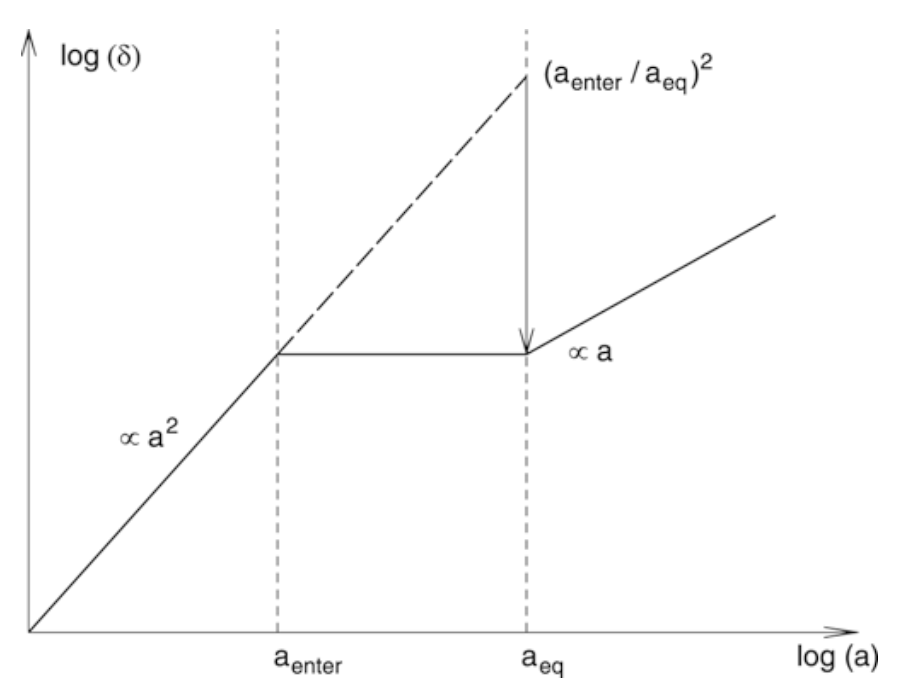
\includegraphics[width=8cm]{figures/cosmology/DensityContrast.png}}
\end{figure}

{\noindent}In linear perturbation theory, fluctuations grow at the same rate on all scales, or for all wave numbers, independent of each other. This applies not only in the Newtonian case, but also remains valid in the framework of General Relativity as long as the fluctuation amplitudes are small. Therefore, the behavior on any (comoving) length-scale can be investigated independently of the other scales. At very early times, perturbations with a comoving scale $L$ are larger than the (comoving) horizon, and only for $z<z_\mathrm{enter}(L)$ does the horizon become larger than the considered scale $L$. Here, $z_\mathrm{enter}(L)$ is defined as the redshift at which the (comoving) horizon equals the (comoving) length-scale $L$,

\begin{align*}
    r_\mathrm{H,com}(z_\mathrm{enter}(L)) = L ~ [{\rm Mpc}].
\end{align*}

{\noindent}It is common to say that at $z_\mathrm{enter}(L)$ the perturbation under consideration `enters the horizon', whereas actually the process is the opposite -- the horizon outgrows the perturbation. Relativistic perturbation theory shows that density fluctuations of scale $L$ grow as long as $L>r_\mathrm{H,com}$, namely $\propto a^2$ if radiation dominates (thus, for $z>z_\mathrm{rm}$), or $\propto a$ if matter dominates (i.e., for $z<z_\mathrm{rm}$). Free-streaming particles or pressure gradients cannot impede the growth on scales larger than the horizon length because, according to the definition of the horizon, physical interactions (which pressure or free-streaming particles would be) cannot extend to scales larger than the horizon size.

{\noindent}The evolution of density fluctuations of baryons differs from that of DM. The reason for this is essentially the interaction of baryons with photons: although matter dominates the Universe for $z<z_\mathrm{rm}$, the energy density of baryons remains smaller than that of the photons for a longer time after recombination begins, as can be seen as follows: the baryon-to-photon density ratio is

\begin{align*}
    \frac{\rho_b}{\rho_\gamma} = \frac{\Omega_ba^{-3}}{\Omega_\gamma a^{-4}} = a\frac{\Omega_b\Omega_m\Omega_r}{\Omega_m\Omega_r\Omega_\gamma} = 1.68\frac{a}{a_\mathrm{rm}}\frac{\Omega_b}{\Omega_m} \sim 0.28\frac{a}{a_\mathrm{rm}} ~ [{\rm dimensionless}].
\end{align*}

{\noindent}Hence, if radiation-matter equality happens at $z_\mathrm{rm}\sim3,000$, then the photon density is larger than that of the baryons for $z\gtrsim800$.

{\noindent}Since photons and baryons interact with each other by photon scattering on free electrons, which again are tightly coupled electromagnetically to protons and helium nuclei, baryons and photons are strongly coupled before recombination, and form a single fluid. Due to the presence of photons, this fluid has a strong pressure, which prevents it from falling into potential wells formed by the dark matter. Thus, the pressure prevents strong inhomogeneities of the baryon-photon fluid.

{\noindent}To discuss the evolution of baryon perturbations in a bit more detail, we consider again a perturbation of comoving scale $L$. As long as the perturbation is larger than the horizon size, pressure effects can not affect the behavior of the fluid, and thus baryons and photons behave in the same way as the dark matter -- the amplitude of their perturbations grow. As soon as the perturbation enters the horizon, the situation changes. Although the baryons are gravitationally pulled into the density maxima of the dark matter, pressure provides a restoring force which acts against a compression of the baryon-photon fluid. As a results, this fluid will develop sound waves.

{\noindent}The maximum distance sound waves can
travel up to a given epoch is called the sound horizon.
Loosely speaking, it is given by the product of the sound
speed and the cosmic time. The sound speed in this photon-dominated fluid is given by $c_s\approx c/\sqrt{3}$. Thus, the sound horizon is about a factor of $\sqrt{3}$ smaller than the event horizon. As soon as a perturbation enters the sound horizon, the amplitude of the baryon-photon fluctuations can not grow anymore; instead, the undergo damped oscillations.

{\noindent}The adiabatic sound speed $c_s$ of a fluid is given in general by

\begin{align*}
    c_s = \sqrt{\frac{\partial P}{\partial\rho}} ~ [{\rm m\,s^{-1}}].
\end{align*}

{\noindent}The pressure of the fluid is generated by the photons, $P=c^2\rho_\gamma/3=c^2\rho_c\Omega_\gamma$, and the density is the sum of that of baryons and photons, $\rho=(\Omega_ba^{-3}+\Omega_\gamma a^{-4})\rho_c$. Thus, the sound velocity is

\begin{align*}
    c_s &= \sqrt{\frac{\partial P}{\partial\rho}} \\
        &= \sqrt{\frac{\mathrm{d}P/\mathrm{d}a}{\mathrm{d}\rho/\mathrm{d}a}} \\
        &= \frac{c}{\sqrt{3}}\sqrt{\frac{4\Omega_\gamma a^{-5}}{3\Omega_ba^{-4}+4\Omega_\gamma a^{-5}}} \\
        &= \frac{c}{\sqrt{3(1+\mathcal{R})}} ~ [{\rm m\,s^{-1}}],
\end{align*}

{\noindent}where $\mathcal{R}$ is defined to be

\begin{align*}
    \mathcal{R} = \frac{3}{4}\frac{\rho_b}{\rho_\gamma} = \frac{3}{4}\frac{\Omega_b}{\Omega_\gamma}a ~ [{\rm dimensionless}].
\end{align*}

{\noindent}Note that $\mathcal{R}$ is smaller than unity until recombination, and thus $c_s\approx c/\sqrt{3}$ provides a reasonable first approximation.

{\noindent}At recombination, the free electrons recombined with the hydrogen and helium nuclei, after which there are essentially no more free electrons which couple to the photon field. Hence, after recombination the baryon fluid lacks the pressure support of the photons, and the sound speed drops to zero -- the sound waves do no longer propagate, but get frozen in. Now the baryons are free to react to the gravitational field created by the dark matter inhomogeneities, and they can fall into their potential wells. After some time, the spatial distribution of the baryons is essentially the same as that of the dark matter.

{\noindent}Hence, there is a maximum wavelength of the sound waves, namely the (comoving) sound horizon at recombination,

\begin{align*}
    r_\mathrm{H,com}(z) = \int\limits_0^t \frac{c\mathrm{d}t}{a(t)} = \int\limits_0^{(1+z)^{-1}} \frac{c\mathrm{d}a}{a^2H(a)} = \int\limits_0^{a_\mathrm{rec}} \frac{c\mathrm{d}a}{\sqrt{3(1+\mathcal{R})}a^2H(a)} ~ [{\rm Mpc}],
\end{align*}

{\noindent}where we exchanged the speed of light by the speed of sound.

{\noindent}Figure \ref{fig:perturbationevolution} illustrates the physical significance of this length scale, showing the time evolution of an initial density peak of all four components in the Universe. The length scale $r_s$ is the distance the baryon-photon fluid propagates outwards from the initial density peak before baryons and photons decouple, after which the density perturbation of baryons gets frozen. The x-axis shows the comoving radial coordinate, the y-axis displays the density, multiplied by (radius)$^2$. The different snapshots show the spatial distribution of the various species at later epochs. In particular, because the region is overdense in photons, it is overpressured relative to its surroundings. This overpressure must equilibrate by driving a spherical sound wave out into the baryon-photon plasma which propagates at the speed of sound, $c_s\approx c/\sqrt{3}$. Neutrinos freely stream out of the perturbation at the speed of light. The photon and baryons are strongly coupled before recombination, and thus have the same spatial distribution. At the time of decoupling, the wave stalls as the pressure supplying the photons escape and the sound speed plummets. One ends up with a CDM overdensity at the center and a baryon overdensity in a spherical shell $150$ comoving megaparsecs in radius for the concordance cosmology. At $z\ll10^3$, both of these overdensities attract gas and CDM to them, seeding the usual gravitational instability. However, some of the matter also falls into the density peaks (in the example of this figure, it is an overdense spherical shell) created by baryons, whereas the density profile of neutrinos and photons becomes flat. At late times, the distributions of baryons and dark matter become identical (before the onset of non-linear processes such as halo formation). The central density peak, and the secondary peak have a well-defined separation, given by the distance a sound wave could travel before the baryons decoupled from the photons. Galaxies are more likely to form in these overdensities. The radius of the sphere marks a preferred separation of galaxies, which we quantify as a peak in the correlation function on this scale.

{\noindent}The Universe is of course a superposition of these point-like perturbations, but as the perturbation theory is exquisitely linear at high redshift, we can simply add the solutions. The width of the acoustic peak is set by three factors: silk damping due to photons leaking out of the sound wave, adiabatic broadening of the wave as the sound speed changes because of the increasing inertia of the baryons relative to the photons, and the correlations of the initial perturbations.

\begin{figure}[t!]
    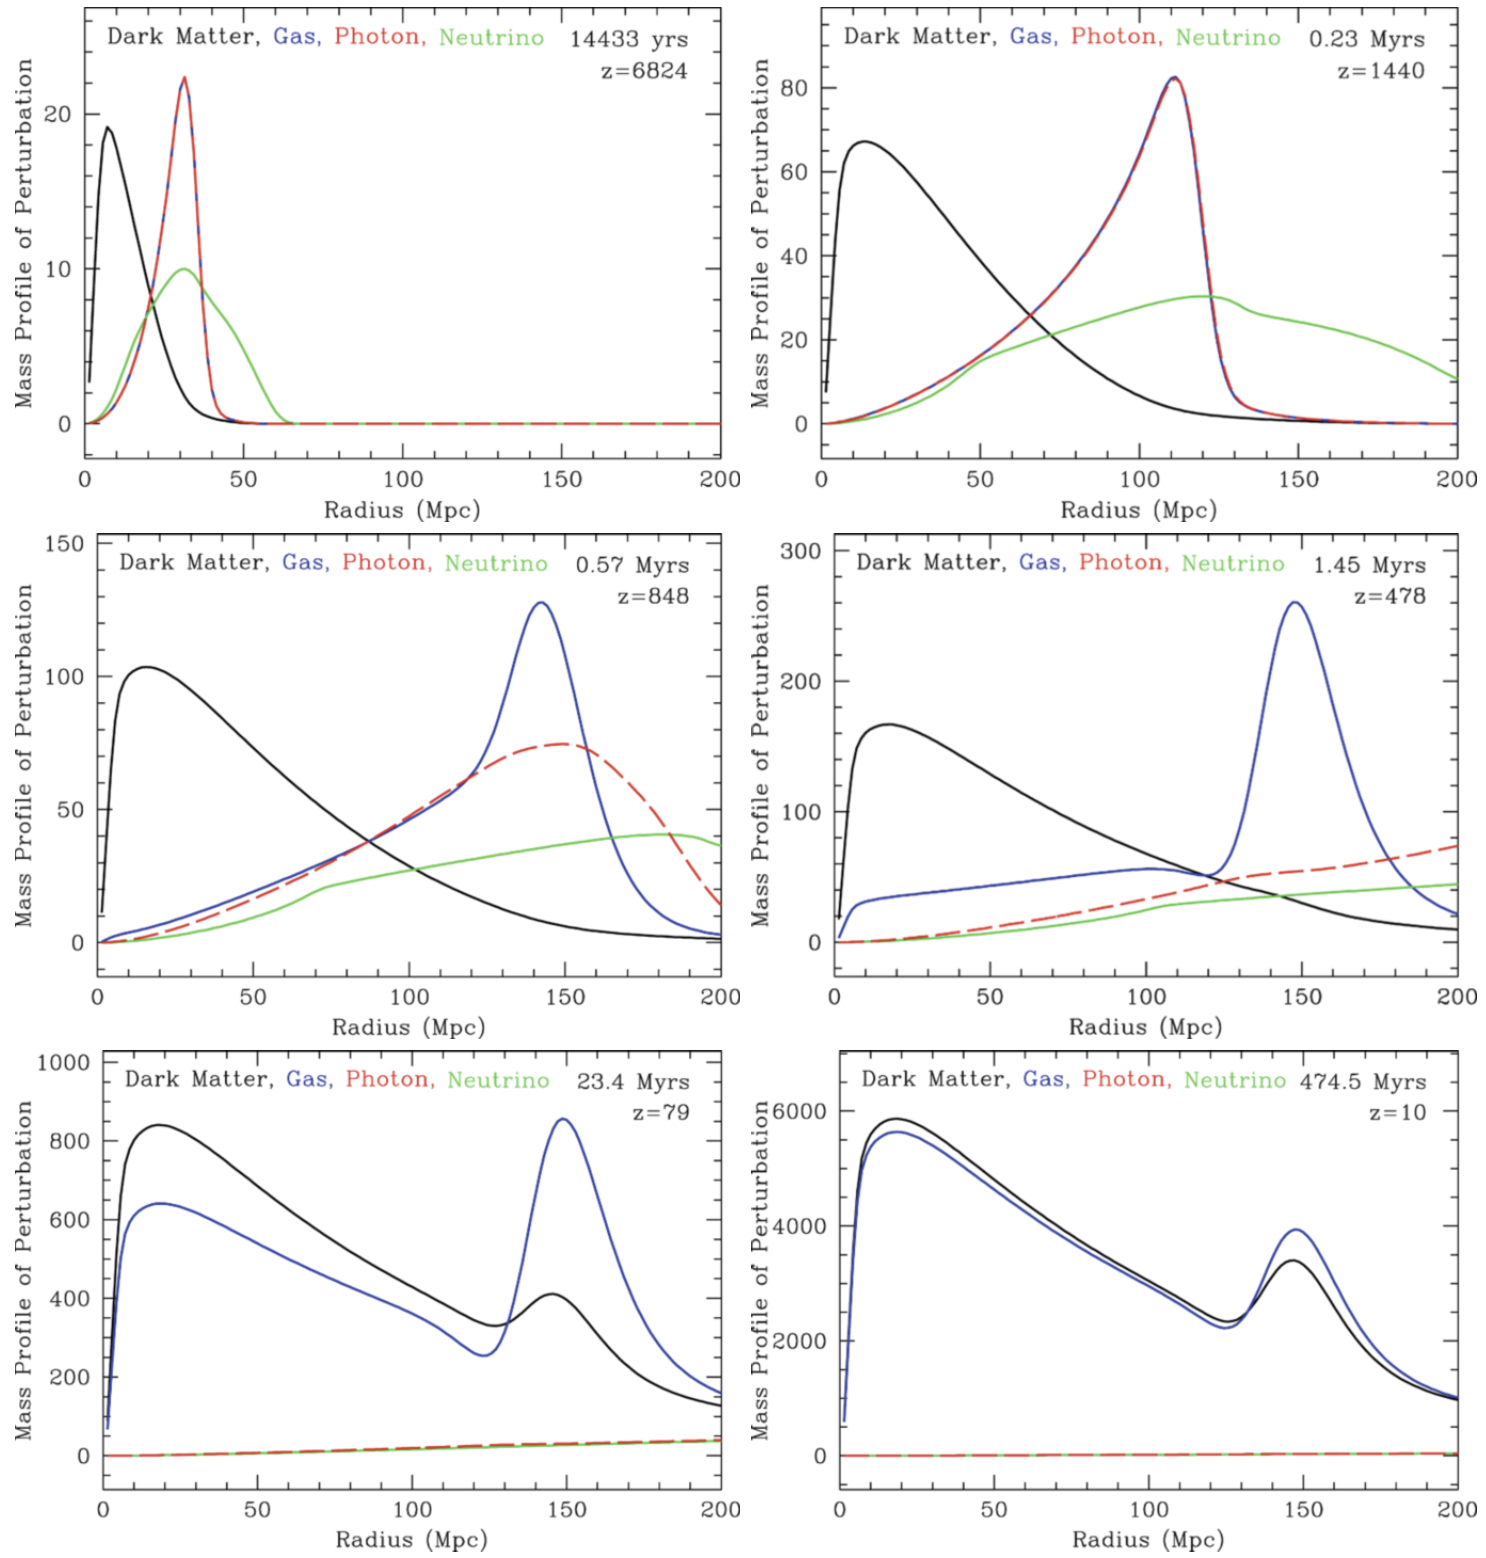
\includegraphics[width=15cm]{figures/cosmology/PerturbationEvolution.png}
    \centering
    \caption{\footnotesize{Evolution in time of an initial density peak in all components of the cosmic matter. \textit{Top left}: Near the initial time, the photons and baryons travel outward as a pulse. \textit{Top right}: Approaching recombination, one can see the wake in the cold dark matter raised by the outward-going pulse of baryons and relativistic species. \textit{Middle left}: At recombination, the photons leak away from the baryonic perturbation. \textit{Middle right}: With recombination complete, we are left with a CDM perturbation toward the center and a baryonic perturbation in a shell. \textit{Bottom left}: Gravitational instability now takes over, and new baryons and dark matter are attracted to the overdensities. \textit{Bottom right}: At late times, the baryonic fraction of the perturbation is near the cosmic value, because all of the new material was at the cosmic mean. Source: D.J. Eisenstein et al. 2007, On the Robustness of the Acoustic Scale in the Low-Redshift Clustering of Matter, ApJ 664, 660, p. 662, Fig. 1. Figure taken from Schneider (2006).}}
    \label{fig:perturbationevolution}
\end{figure}

{\noindent}There are some other interesting aspects of the physics of this epoch that are worth mentioning. First is that the outgoing wave does not actually stop at $z\sim10^3$ but instead slows around $z\sim500$. This is partially due to the fact that decoupling is not coincident with recombination but is also because the coupling to the growing mode is actually dominated by the velocity field, rather than the density field, at $z\sim10^3$. In other words, the compressing velocity field in front of the wave actually keys the instability at a later time.

{\noindent}Two other aspects that may be surprising at first
glance are that the outgoing pulse of neutrino overdensity does not actually remain as a delta function, as one might expect for a population traveling radially outward at the speed of light, and that the CDM perturbation does not remain at the origin, as one would expect for a cold species. Both of these effects are due to a hidden assumption in the initial conditions: although the density field is homogeneous everywhere but the origin, the velocity field cannot be for a growing mode. To keep the bulk of the Universe homogeneous while growing a perturbation at the origin, matter
must be accelerating toward the center; this acceleration is supplied by the gravitational force from the central overdensity. However, in the radiation-dominated epoch the outward-going pulse of neutrinos and photons is carrying away most of the energy density of the central perturbation. This outward-going pulse decreases the acceleration, causing the inward flow of the homogeneous bulk to deviate from the divergenceless flow and generating the behavior of the CDM and neutrinos mentioned above. Essentially,
the outgoing shells of neutrinos and photons raise a wake in the homogeneous distribution of CDM away from the origin
of the perturbation.

{\noindent}The smoothing of the CDM overdensity from a delta function at the origin is the famous small-scale damping of the CDM power spectrum in the radiation-dominated epoch. The overdensity raised decreases as a function of radius because the radiation is decreasing in energy density relative to the inertia of the CDM; in the matter-dominated regime, the outward-going radiation has no further effect. A Universe with more radiation causes a larger effect that extends to larger radii; this corresponds to the shift in the CDM power spectrum with the matter-to-radiation ratio.

{\noindent}Returning to the major conceptual point, that of the shell of overdensity left at the sound horizon, we see immediately that the sound horizon provides a standard ruler. The radius of the shell depends simply on the sound speed and the amount of propagation time. The sound speed is set by the balance of radiation pressure and inertia from the baryons; this is controlled simply by the baryon-to-photon ratio, which is $\Omega_bh^2$. The propagation time depends on the expansion rate in the matter-dominated and radiation-dominated regimes; this in turn depends on the redshift of matter-radiation equality, which depends only on $\Omega_mh^2$ for the standard assumption of the radiation density (i.e., the standard cosmic neutrino and photon backgrounds and nothing else).

{\noindent}The sound waves in the baryon-photon fluid, the baryonic acoustic oscillations (BAOs), are observable today. Since at recombination, the photons interacted with matter for the last time, the CMB radiation provides us with a picture of the density fluctuations at the epoch of recombination. Our observable cosmic microwave sky essentially is a picture of a two-dimensional cut at fixed time (the time of last scattering) through the density field of the baryons. A cut through an ensemble of sound waves shows an instantaneous picture of these waves. Hence, they are expected to be visible in the temperature distribution of the CMB. This is indeed the case: these BAOs imprint one of the most characteristic features on the CMB anisotropies. Since the sound waves are damped once they are inside the sound horizon, the largest amplitude waves are those whose wavelength equals the sound horizon at recombination.

{\noindent}We have argued that the baryons, once they are no longer coupled to radiation and thus become pressureless, fall into the potential wells of the dark matter. This happens because the dark matter fluctuations can grow while the baryonic fluctuations could not due to the photon pressure, and because the mean density of dark matter is substantially larger than that of the baryons. This is almost the full story, but not entirely: baryons make about 15\% of the total matter density, and are therefore not negligible. After recombination, the BAOs are frozen, like standing waves, and thus the total matter fluctuations are a superposition of the dark matter inhomogeneities and these standing waves. Whereas the dark matter dominates the density fluctuations, a small fraction of the matter also follows the inhomogeneities created by the standing waves. Since these waves have a characteristic length scale (the sound horizon at recombination) this characteristic length scale should be visible in the properties of the matter distribution even today. The correlation function of galaxies contains a characteristic feature at the length scale $r_s$. Hence, relics of the sound waves in the pre-recombination era are even visible in the current Universe. The effects of the BAOs are included in the transfer function $T(k)$, which thus shows some low-amplitude oscillations, often called `wiggles'.

{\noindent}The distance that acoustic waves can propagate in the first million years of the Universe is measurable not only in the cosmic microwave background (CMB) anisotropies but also in the late-time clustering of galaxies.

\subsubsection{Follow-up Questions}

\begin{itemize}
    \item How do we observe the power spectrum?
    \item What is its relation to BAOs and the $C_\ell$ power spectrum?
    \item Do we see super-horizon modes (modes larger than the Universe's event horizon) in the evolved matter power spectrum?
    \item What actually causes the damping during the radiation-dominated era?
    \item Why do modes outside the horizon grow?
    \item What is Silk damping and what is physically happening?
    \item Why does Silk damping only affect small modes?
    \item How do baryon and photon perturbations grow?
    \item How does this relate to whether structure grows in a top-down or bottom-up approach?
\end{itemize}

% --------------------------------------------------------------
%
%                           4. 
%
% --------------------------------------------------------------

\newpage
\subsection{Question 4}

State and explain three key pieces of evidence for a Big Bang origin for the observable Universe.

\subsubsection{Short answer}

The success of the Big Bang (BB) rests on three observational pillars:

\begin{enumerate}
    \item Hubble's Law exhibiting expansion: The first key observation to the modern era of cosmology that the Universe is expanding. If the Universe is expanding at the present time, then by `turning back the clock' the Universe must have been much smaller in the past. Hence, the BB.
    \item Light element abundances which are in accord with Big Bang nucleosynthesis: When the Universe was still a very hot plasma, the extreme radiation field ensured that any nucleus produced would be immediately photoionized by a high energy photon. As the Universe cooled (via expansion) well below the typical binding energies of nuclei, light elements began to form. Knowing the conditions of the early Universe and the relevant cross sections, one can calculate the expected primordial abundances of these light elements. Such predictions are consistent with measurements.
    \item The blackbody radiation left over from the first few hundred thousand years, the cosmic microwave background: The fact that the early Universe was very hot and dense meant that the baryonic matter was well coupled with the radiation field implying thermal equilibrium (TE) of photons. In TE, photons should follow the blackbody (or Planck) function in which the energy density is only dependent on temperature. As it turns out, the CMB radiation is the most accurate BB curve yet to be measured!
\end{enumerate}

\subsubsection{Additional context}

1. \textbf{Hubble's Law}

{\noindent}We have good evidence that the Universe is expanding. This means that early in its history, the distances between galaxies was smaller than it is today. It's convenient to describe this expansion effect by introducing the \textbf{scale factor} $a$, whose present value is equal to one ($a(t_0)\equiv1$). At earlier times, $a$ was much smaller than it is today -- hence, the Big Bang. 

{\noindent}The first key observation to the modern era of cosmology was the discovery of an expanding Universe. This is popularly credited to Edwin Hubble in 1929, but in fact the honour lies with Vesto Slipher more than 10 years earlier. Slipher was measuring spectra of nebulae whose nature was still under hot debate at that time. Observations of Hubble settled this debate in 1924 when he discovered \textit{Cepheid variables} in M31 (Andromeda) establishing a distance of roughly $1\,{\rm Mpc}$. More than a decade earlier in 1913, Slipher had measured the spectrum of M31 and found that it was approaching Earth at a velocity of over $200\,{\rm km\,s^{-1}}$. Over the next decade, he measured Doppler shifts for dozens of galaxies: with only a few exceptions, they were redshifted. By the time Hubble arrived, the basics of relativistic cosmology were already worked out and predictions existed that galaxy redshifts should increase with distance. It's hard to know how much these influenced Hubble, but by 1929 he had obtained Cepheid distances towards 24 galaxies along with their redshifts and claimed that they followed the empirical linear relationship:

\begin{align*}
    v = H_0 d ~ [{\rm km\,s^{-1}}],
\end{align*}

{\noindent}citing theoretical predictions as a possible explanation. At the time, Hubble estimated $H_0 \approx 500\,{\rm km\,s^{-1}\,Mpc^{-1}}$ because his calibration of Cepheid variables was in error. The best modern value is currently $H_0 = 70\,{\rm km\,s^{-1}\,Mpc^{-1}}$.

\begin{figure}[h]
    \floatbox[{\capbeside\thisfloatsetup{capbesideposition={right,center},capbesidewidth=4cm}}]{figure}[\FBwidth]
    {\caption{\footnotesize{The original Hubble diagram (Hubble, 1929). Velocities of distant galaxies (units should be ${\rm km\,s^{-1}}$) are plotted vs distance (units should be ${\rm Mpc}$). Solid (dashed) line is the best fit to the filled (open) points which are corrected (uncorrected) for the Sun's motion. Image taken from Dodelson (2003).}}
    \label{fig:hubblediagram}}
    {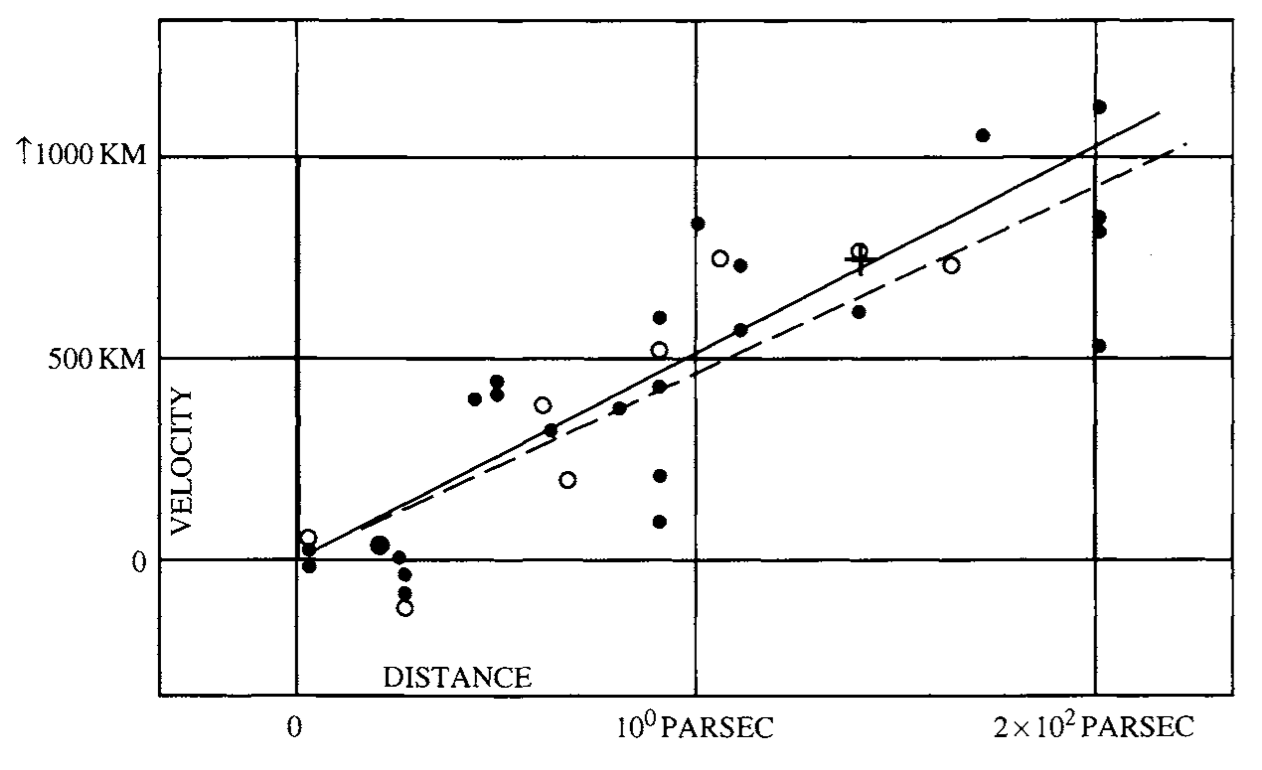
\includegraphics[width=12cm]{figures/cosmology/HubbleDiagram.png}}
\end{figure}

{\noindent}Recall that the wavelength of light or sound emitted from a receding object is stretched out (i.e., Doppler shifted) so that the observed wavelength is larger than the emitted one. It is convenient to define this stretching factor as the redshift $z$:

\begin{align*}
    1+z \equiv \frac{\lambda_0}{\lambda} = \frac{1}{a} ~ [{\rm dimensionless}],
\end{align*}

{\noindent}or

\begin{align*}
    (1+z)^{-1} \equiv \frac{\lambda}{\lambda_0} = a ~ [{\rm dimensionless}].
\end{align*}

{\noindent}For low redshifts, the standard Doppler formula applies and $z \sim v/c$. Therefore, a measurement of the amount by which absorption and/or emission lines are redshifted is a direct measure of how fast the structures in which they reside are receding from us. Hubble's diagram is shown in Figure \ref{fig:hubblediagram}, which shows not only that distant galaxies appear to be receding from us, but that the trend increases linearly with distance which is exactly what we would expect for an expanding Universe.

{\noindent}The Hubble diagram is still the most direct evidence we have that the Universe is expanding. Current incarnations use the same principle as the original: find the distance and the redshift of distant objects. Measuring redshifts is straightforward; the hard part is determining distances for objects of unknown intrinsic brightness. One of the most popular techniques is to try to find a standard candle, a class of objects which have the same intrinsic brightness. Any difference between the apparent brightness of two such objects then is a result of their different distances from us. This method is typically generalized to find a correlation between an observable and intrinsic brightness. For example, \textbf{Cepheid variables} are stars for which intrinsic brightness is tightly related to their pulsation period.

\begin{figure}[t!]
    \floatbox[{\capbeside\thisfloatsetup{capbesideposition={right,top},capbesidewidth=4cm}}]{figure}[\FBwidth]
    {\caption{\footnotesize{\\Hubble diagram from distant Type la supernovae. Top panel shows apparent magnitude (an indicator of the distance) vs redshift. Lines show the predictions for different energy contents in the Universe, with $\Omega_M$ the ratio of energy density today in matter compared to the critical density and $\Omega_\Lambda$ the ratio of energy density in a cosmological constant to the critical density. Bottom panel plots the residuals, making it clear that the high-redshift supernovae favor a $\Lambda$-dominated Universe over a matter-dominated one. Figure taken from Dodelson (2003).}}
    \label{fig:hubblediagram_modern}}
    {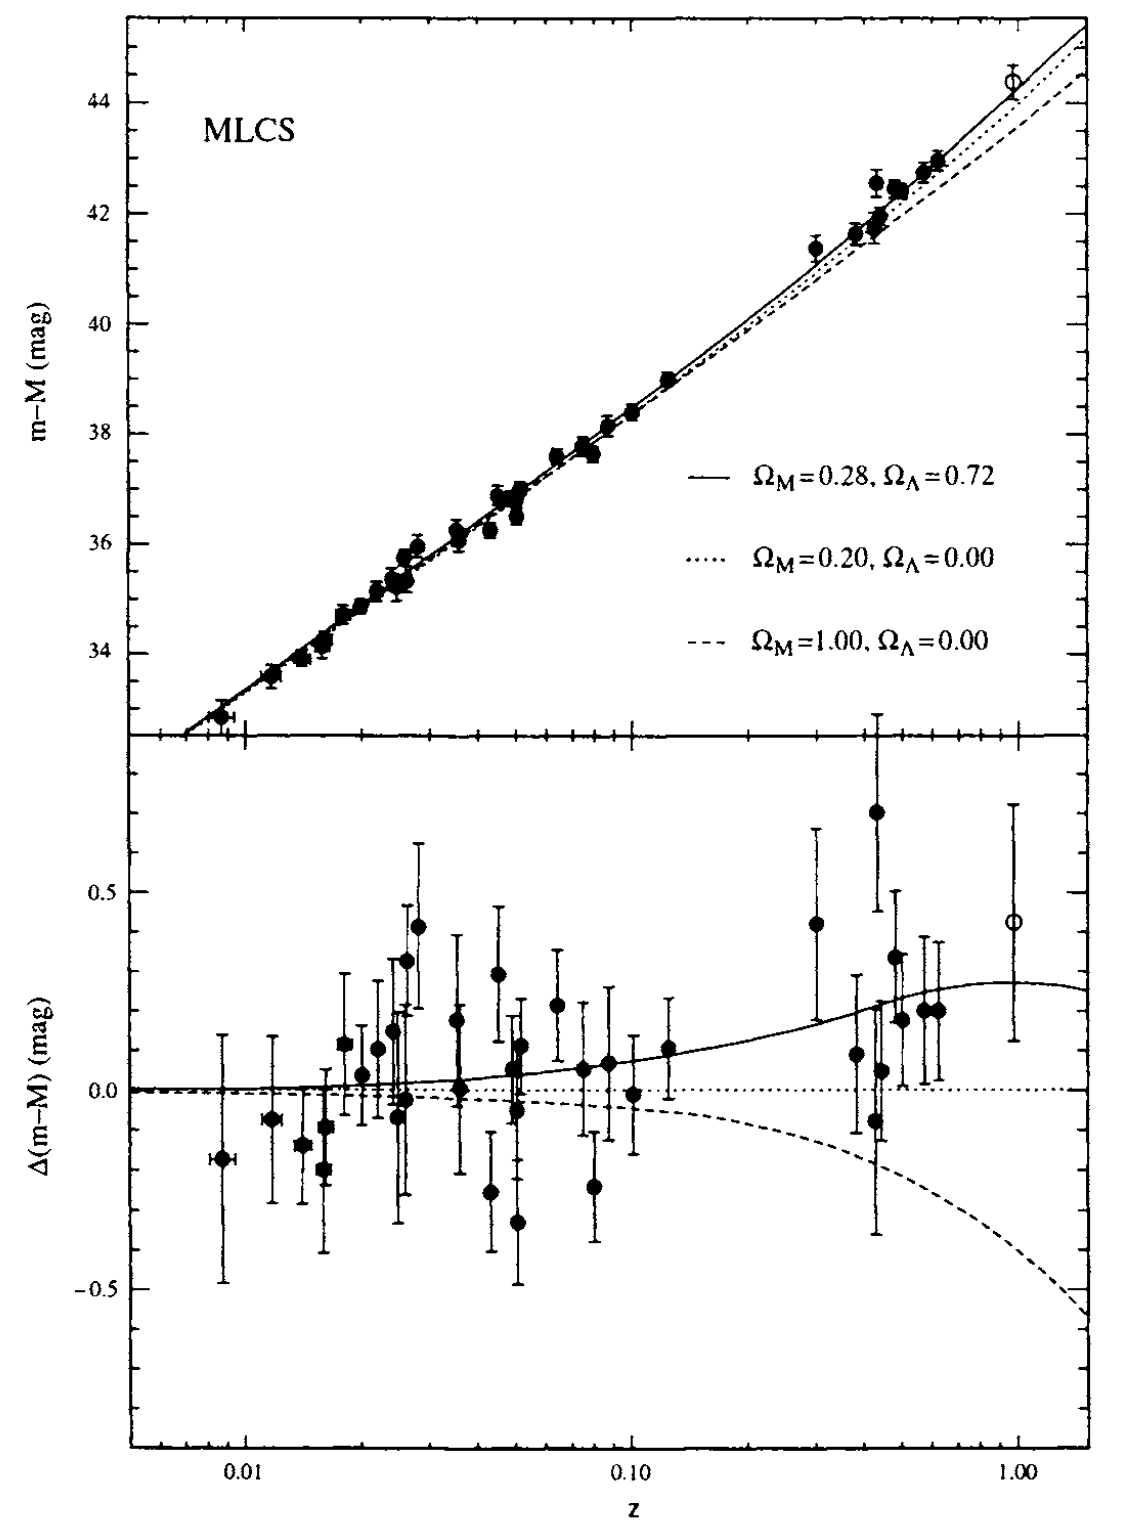
\includegraphics[width=10cm]{figures/cosmology/HubbleDiagram_modern.png}}
\end{figure}

{\noindent}As seen in Figure \ref{fig:hubblediagram_modern}, the standard candle that can be seen at largest distances is a Type la supernova. Since they are so bright, supernovae can be used to extend the Hubble diagram out to very large redshifts (the current record is of order $z\sim1.7$), a regime where the simple Doppler law ceases to work. Figure \ref{fig:hubblediagram_modern} shows a recent Hubble diagram using these very distant objects. The three curves in Figure \ref{fig:hubblediagram_modern} depict three different possibilities: flat matter dominated; open; and flat with a cosmological constant ($\Omega$). The high-redshift data are now good enough to distinguish among these possibilities, strongly disfavoring the previously favored flat, matter-dominated Universe. The current best fit is a Universe with about 70\% of the energy in the form of a cosmological constant, or some other form of dark energy.

{\noindent}2. \textbf{Big Bang Nucleosynthesis}

{\noindent}When the Universe was much hotter and denser, when the temperature was of order an ${\rm MeV/k_B}$, there were no neutral atoms or even bound nuclei. The vast amounts of radiation in such a hot environment ensured that any atom or nucleus produced would be immediately destroyed by a high energy photon. As the Universe cooled well below the binding energies of typical nuclei, light elements began to form. Knowing the conditions of the early Universe and the relevant nuclear cross-sections, we can calculate the expected primordial abundances of all the elements.

\begin{figure}[h]
    \floatbox[{\capbeside\thisfloatsetup{capbesideposition={left,center},capbesidewidth=4cm}}]{figure}[\FBwidth]
    {\caption{\footnotesize{BBN predictions of the primordial abundances of light elements as a function of today’s baryon density ($\rho_{b,0}$ lower axis) and the corresponding density parameter $\Omega_b$ where $h=0.65$ was assumed. The vertical extent of the rectangles marks the measured values of the abundances (top: He$^4$, center: D, bottom: Li$^7$). The horizontal extent results from the overlap of these intervals with curves computed from theoretical models. The ranges in $\Omega_b$ that are allowed by these three species do overlap, as is indicated by the vertical strip. The deuterium measurements yield the most stringent constraints for $\Omega_b$. Figure taken from Schneider (2006).}}
    \label{fig:bbn_prediction}}
    {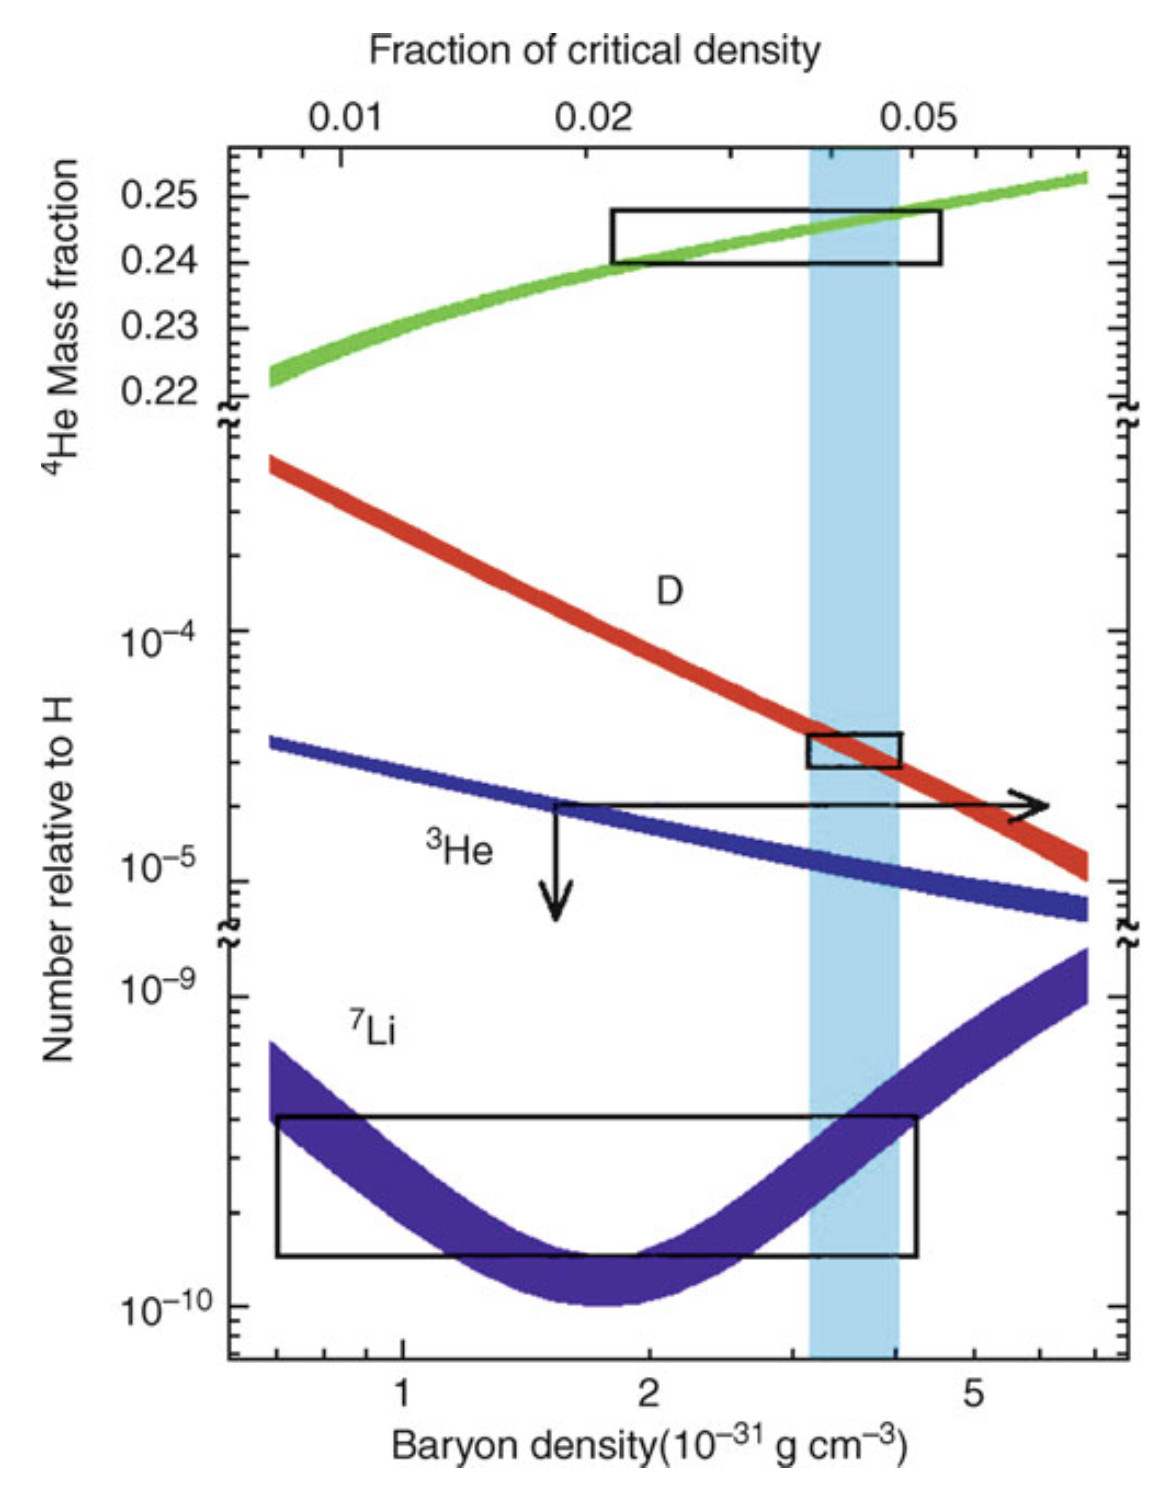
\includegraphics[width=10cm]{figures/cosmology/BBN_prediction.png}}
\end{figure}

{\noindent}Figure \ref{fig:bbn_prediction} shows the predictions of Big Bang Nucleosynthesis (BBN) for the light element abundances\footnote{Recall nuclear notation: The 4 in $^4$He refers to the total number of nucleons (protons and neutrons). So $^4$He has two neutrons and two protons, while $^3$He has two protons and one neutron.}. The boxes and arrows show the current estimates for the light element abundances. These are consistent with the predictions, and this consistency test provides yet another ringing confirmation of the Big Bang. The theoretical predictions depend on the density of protons and neutrons at the time of nucleosynthesis. The combined proton plus neutron density is called the \textbf{baryon density} ($\rho_b$) since both protons and neutrons have baryon number one and these are the only baryons around at the time. Thus, BBN gives us a way of measuring the baryon density in the Universe. Since we know how those densities scale as the Universe evolves (they fall as $a^{-3}$), we can turn the measurements of light element abundances into measures of the baryon density today.

{\noindent}In particular, the measurement of primordial deuterium pins down the baryon density extremely accurately to only a few percent of the critical density. Ordinary matter (baryons) contributes at most 5\% of the critical density (i.e., $\Omega_b = 0.005$). Since the total matter density today is almost certainly larger than this -- direct estimates give values of order 20-30\% — nucleosynthesis provides a compelling argument for non-baryonic dark matter.

\begin{figure}[h]
    \floatbox[{\capbeside\thisfloatsetup{capbesideposition={left,center},capbesidewidth=4cm}}]{figure}[\FBwidth]
    {\caption{\footnotesize{Spectrum from a distant QSO (Buries, Nollett, and Turner, 1999). Absorption of photons with rest wavelength $1216$ {\AA} corresponding to the (n = 1) to (n = 2) state of hydrogen is redshifted up to $1216(1+3.572)$ \AA. Bottom panel provides details of the spectrum in this range, with the the presence of deuterium clearly evident. Figure taken from Dodelson (2003).}}
    \label{fig:deuterium}}
    {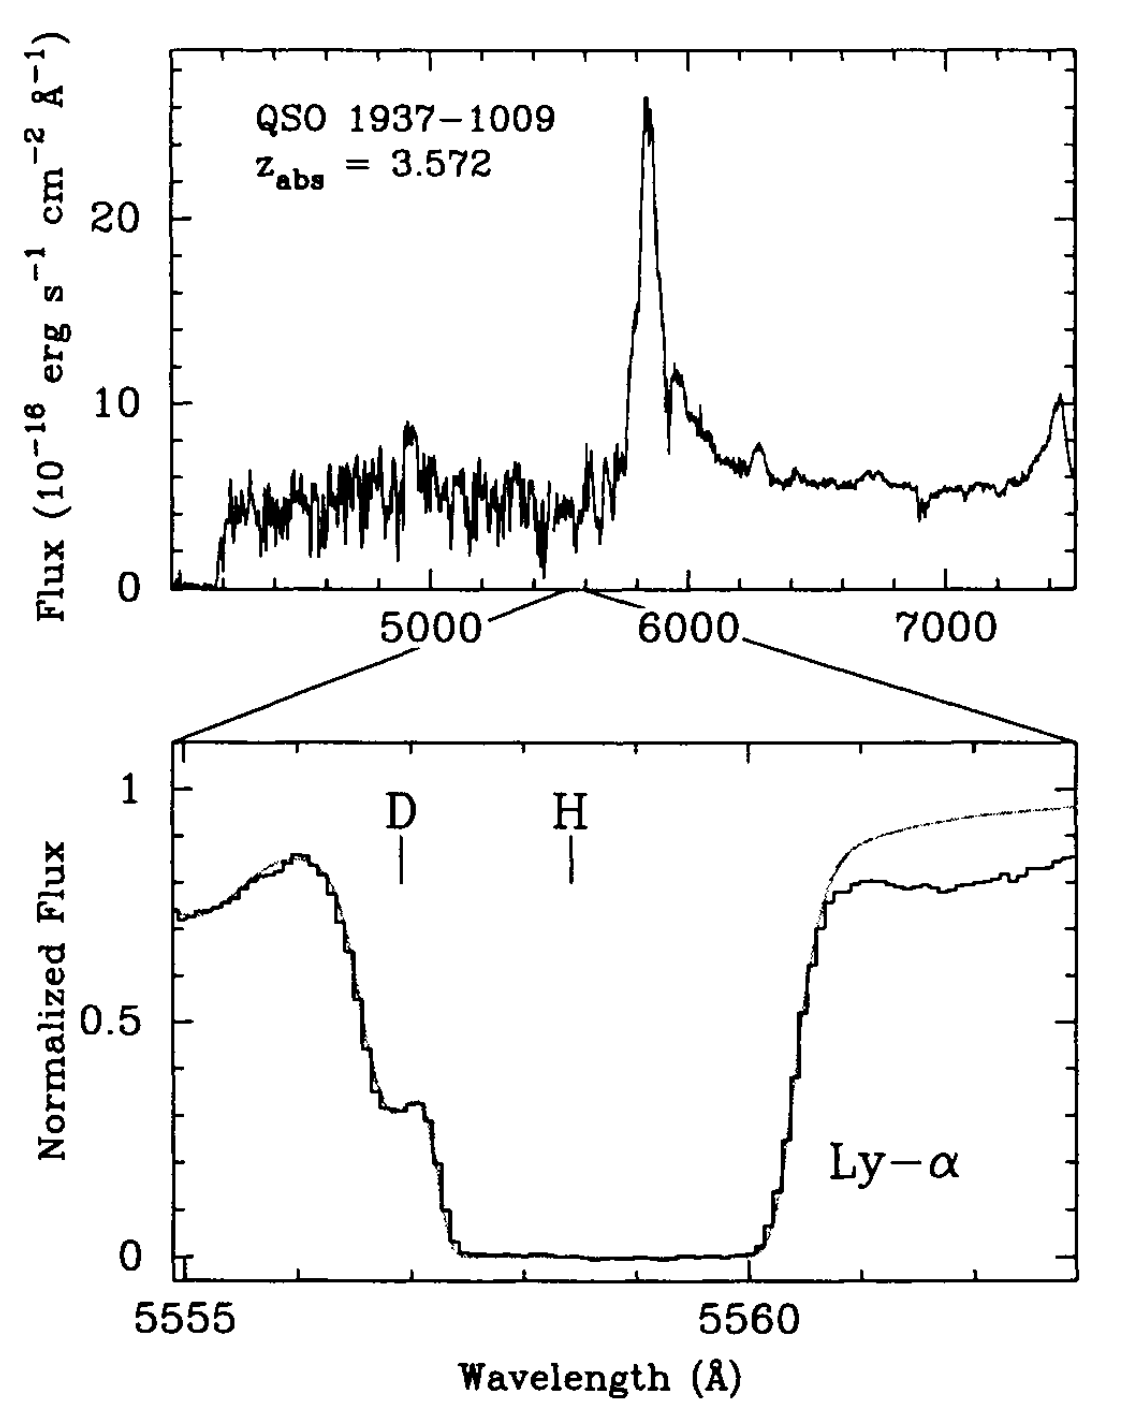
\includegraphics[width=10cm]{figures/cosmology/deuterium.png}}
\end{figure}

{\noindent}The deuterium measurements (Buries \& Tytler, 1998) are the new developments in the field. These measurements are so exciting because they explore the deuterium abundance at redshifts of order 3-4, well before much processing could have altered the primordial abundances. Figure \ref{fig:deuterium} shows one such detection. The basic idea is that light from distant QSOs is absorbed by intervening neutral hydrogen systems. The key absorption feature arises from transition from the ground state (n=1) of hydrogen to the first excited state (n = 2), requiring a photon with wavelength $\lambda = 1215.7$ \AA. Since photons are absorbed when exciting hydrogen in this fashion, there is a trough in the spectrum at {\AA}, redshifted by a factor of $(1+z)$. The corresponding line from deuterium should be (i) shifted over by $0.33(1+z)$ {\AA} and (ii) much less damped since there is much less deuterium. Figure \ref{fig:deuterium} shows just such a system; there are now half a dozen with detections precisely in the neighborhood shown in Figure \ref{fig:bbn_prediction}. Note that the steep decline in deuterium as a function of baryon density helps here: even relatively large errors in deuterium measurements translate into small errors on the baryon density.

{\noindent}3. \textbf{Cosmic Microwave Background (CMB)}

{\noindent}The CMB offers us a look at the Universe when it was only $\sim 380,000$ years old. The photons in the CMB last scattered off electrons at $z \sim 1100$; since then they have traveled freely through space. When we observe them today, they literally come from the earliest moments of time. They are therefore the most powerful probes of the early Universe. If an object is opaque then the protons, neutrons, electrons, and photons which it contains frequently interact and attain \textit{thermal equilibrium}. A crucial fact about the CMB is that the collisions between electrons and photons before last scattering ensured that the photons were in equilibrium. That is, they should have a blackbody spectrum. When a system is in thermal equilibrium, the density of photons in the system as a function of photon energy depends only on the system temperature $T$. It doesn't matter whether the system is a tungsten filament or a sphere of ionized hydrogen and helium.

\begin{figure}[h]
    \floatbox[{\capbeside\thisfloatsetup{capbesideposition={right,center},capbesidewidth=4cm}}]{figure}[\FBwidth]
    {\caption{\footnotesize{Intensity of cosmic microwave radiation as a function of wavenumber from Far InfraRed Absolute Spectrophotometer (FIRAS) (Mather et al., 1994), an instrument on the COBE satellite. Hidden in the theoretical blackbody curve are dozens of measured points, all of which have uncertainties smaller than the thickness of the curve! Figure taken from Dodelson (2003).}}
    \label{fig:cmb_cobe}}
    {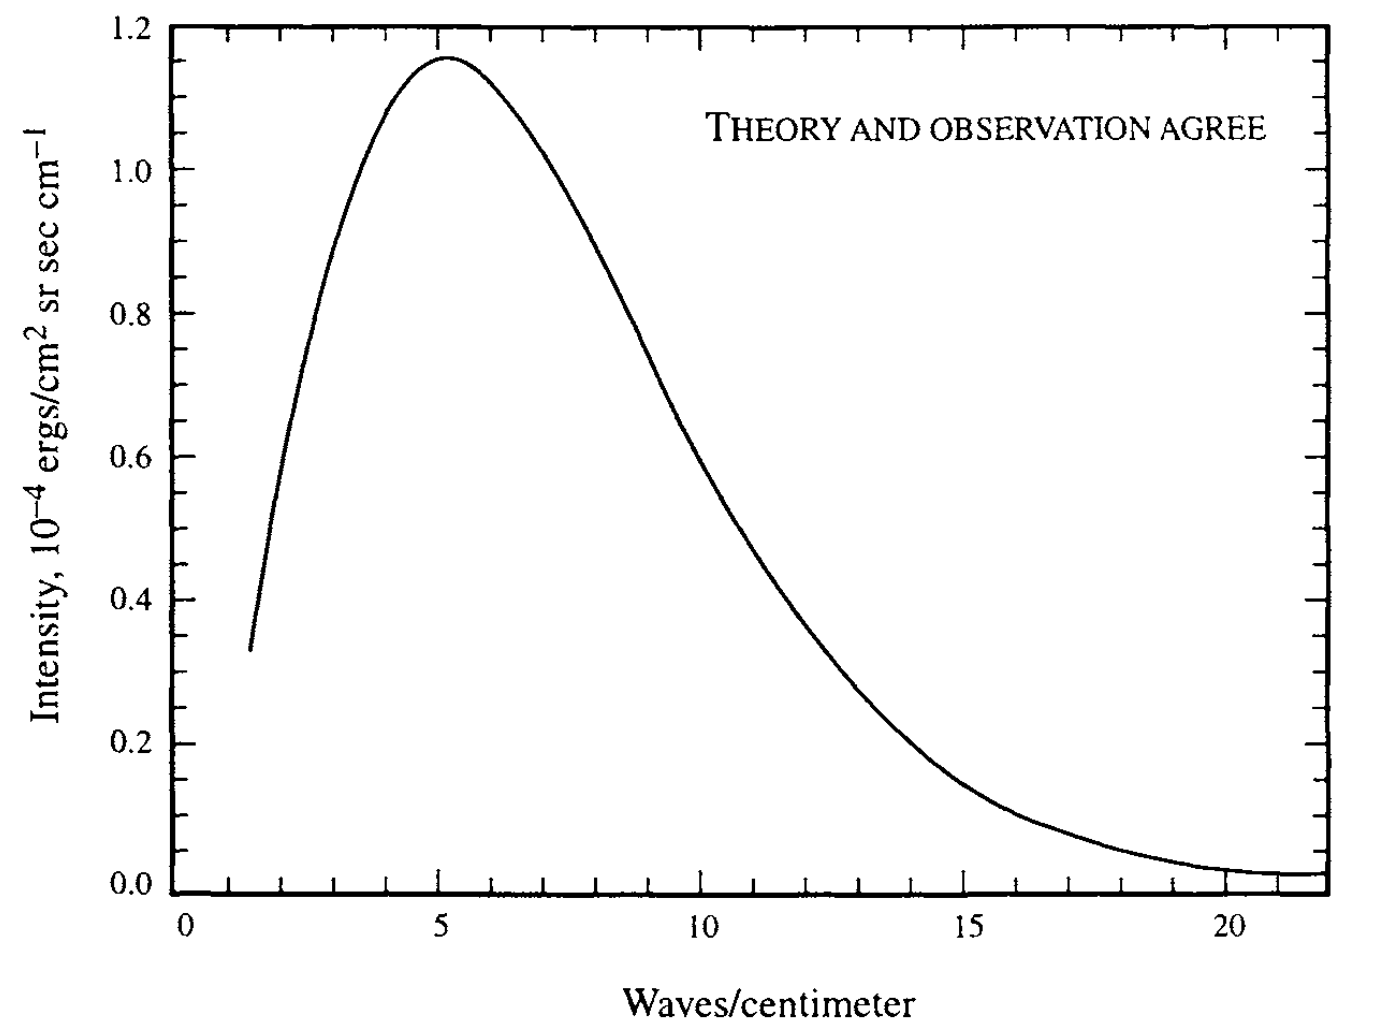
\includegraphics[width=10cm]{figures/cosmology/CMB_COBE.png}}
\end{figure}

{\noindent}The specific intensity of a gas of photons following a blackbody spectrum is called the \textbf{Planck function}:

\begin{align*}
    I_\nu = B_\nu(T) = \frac{2h\nu^3}{c^2} \frac{1}{\exp({h\nu/k_BT}) - 1} ~ [{\rm erg\,s^{-1}\,cm^{-2}\,Hz^{-1}\,sr^{-1}}].
\end{align*}

{\noindent}Figure \ref{fig:cmb_cobe} shows the remarkable agreement between this prediction of Big Bang cosmology and the observations by the FIRAS instrument aboard the COBE spacecraft. We have been told that detection of the $3\,{\rm K}$ background by Penzias and Wilson in the mid-1960s was sufficient evidence to decide the controversy in favor of the Big Bang over the Steady State Universe. Penzias and Wilson, though, measured the radiation at just one wavelength. If even their one-wavelength result was enough to tip the scales, the current data depicted in Figure \ref{fig:cmb_cobe} should send skeptics from the pages of physics journals to the far reaches of radical Internet chat groups.

{\noindent}The photons which make up the cosmic microwave background (CMB) today have a well-measured temperature $T_\mathrm{CMB} = 2.725 \pm 0.002\,{\rm K}$. A photon with an energy $k_BT_\mathrm{CMB}$ today has a wavelength $hc/k_BT_\mathrm{CMB}$. Early on, when the scale factor was smaller than it is today, this wavelength would have been correspondingly smaller. Since the energy of a photon is inversely proportional to its wavelength, the photon energy would have been larger than today by a factor of $1/a$. This argument applied to the thermal bath of photons implies that the temperature of the plasma as a function of time is

\begin{align*}
    T(t) = \frac{T_0}{a(t)} = T_0(1+z) ~ [{\rm K}].
\end{align*}

{\noindent}At early times, then, the temperature was higher than it is today.

{\noindent}The energy density of each component of the Universe is equal to the number density of each corresponding component times its average energy. The primary energy density components of the Universe includes radiation, matter (baryons and dark matter), and dark energy. Since photon energy scales as $a^{-1}$ in addition to the number density which scales as $a^{-3}$, the energy density of radiation should scale as $a^{-4}$. The energy density of non-relativistic particles, such as baryons, have a constant rest mass energy. Since their number density scales inversely proportional to volume, the energy density of matter scales as $a^{-3}$. Dark energy (introduced as a cosmological constant) is believed to have a constant energy density. While matter, and possibly a cosmological constant, dominate the current cosmological landscape, radiation must have been the dominant constituent of the Universe due to its energy density scaling of $a^{-4}$. Figure \ref{fig:energydensityscaling} illustrates how radiation, matter, and the cosmological constant energy density components evolve with time.

\begin{figure}[h]
    \floatbox[{\capbeside\thisfloatsetup{capbesideposition={right,top},capbesidewidth=4cm}}]{figure}[\FBwidth]
    {\caption{\footnotesize{Energy density vs scale factor for different constituents of a flat Universe. Shown are non-relativistic matter, radiation, and a cosmological constant. All are in units of the critical density today. Even though matter and cosmological constant dominate today, at early times, the radiation density was largest. The epoch at which matter and radiation are equal is $a_\mathrm{eq}$. Image taken from Dodelson (2003).}}
    \label{fig:energydensityscaling}}
    {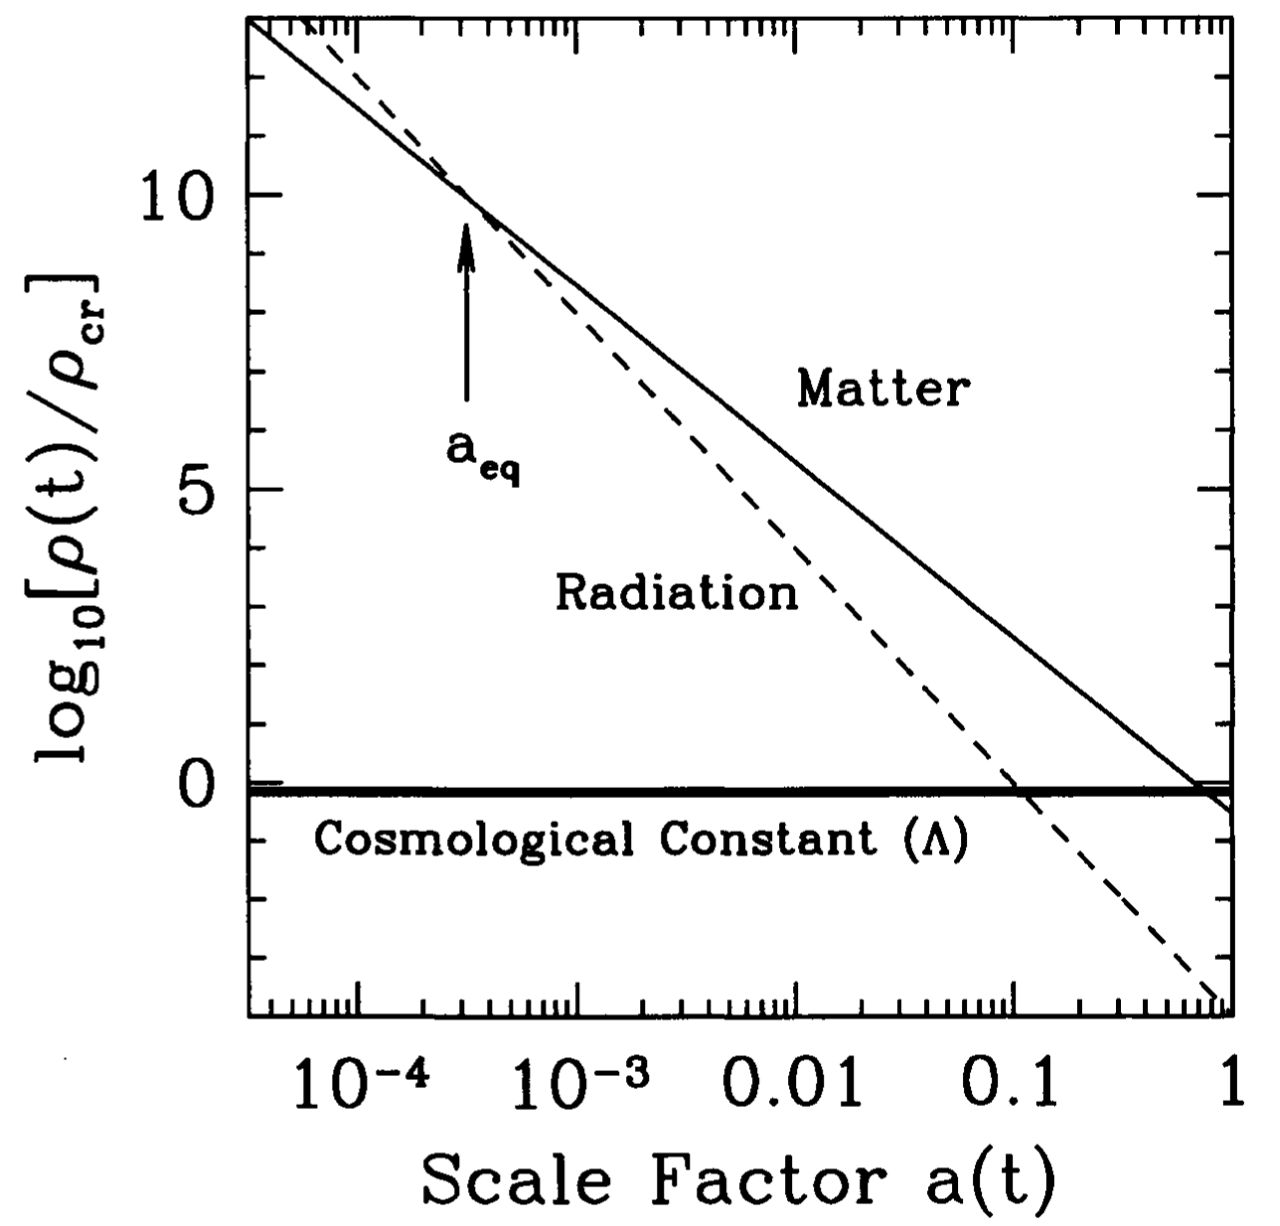
\includegraphics[width=10cm]{figures/cosmology/EnergyDensityScaling.png}}
\end{figure}

{\noindent}The CMB was detected by Arno Penzias \& Robert Wilson in 1965 and were awarded the 1978 Nobel prize in physics; they accomplished this by locating an unaccounted-for source of noise in a radio telescope at Bell Laboratories being used to study our own Galaxy. This excess ``noise'' was isotropic and constant with time, so it couldn't be associated with an isolated celestial source. Wilson and Penzias were puzzled until they were put into touch with Robert Dicke and his research group at Princeton University. Dicke had deduced that the Universe, if it started in a hot dense state, should now be filled with microwave radiation. The timing of the discovery was especially ironic, given that instruments were underway at that time to test the theoretical prediction that such a background should exist.

{\noindent}When the Universe was fully ionized, photons interacted primarily with electrons via Thomson scattering (the low energy limit of Compton scattering): 

\begin{align*}
    \gamma + e^{-} \rightarrow \gamma + e^{-}.
\end{align*}

{\noindent}Thomson scattering is an elastic process whereby energy and momentum are transferred between the photon and electron. The cross-section for Thomson scattering is the Thomson cross-section of 

\begin{align*}
    \sigma_e = 6.65 \times 10^{-29} ~ [{\rm m^2}].
\end{align*}

{\noindent}The mean free path of a photon -- that is, the mean distance it travels before scattering from an electron-- is therefore

\begin{align*}
    \ell_\mathrm{mfp} = \frac{1}{n_e\sigma_e} ~ [{\rm m}].
\end{align*}

{\noindent}When the baryonic component of the Universe is fully ionized, $n_e = n_p = n_b$. Currently, the number density of baryons is $n_{b,0} = 0.22\,{\rm m^{-3}}$. The number density of conserved particles, such as baryons, goes with the scale factor as $1/a^3$, so when the early Universe was fully ionized, the free electron density was

\begin{align*}
    n_e = n_b = \frac{n_{b,0}}{a^3} ~ [{\rm m^{-3}}].
\end{align*}

{\noindent}Since photons travel with speed $c$, the rate at which a photon undergoes scattering interactions is

\begin{align*}
    \Gamma = \frac{c}{\ell_\mathrm{mfp}} = n_e\sigma_ec ~ [{\rm s^{-1}}].
\end{align*}

{\noindent}Using the fact that $n_e = n_b = n_{b,0}/a^3$ for a fully-ionized Universe,

\begin{align*}
    \Gamma = \frac{n_{b,0}\sigma_ec}{a^3} = \frac{4.4\times10^{-21}}{a^3} ~ [{\rm s^{-1}}].
\end{align*}

{\noindent}The photons remain coupled to the electrons as long as their scattering rate, $\Gamma$, is larger than $H$, the rate at which the Universe expands; this is equivalent to saying that their mean free path $\ell_\mathrm{mfp}$ is shorter than the Hubble distance $c/H$.

{\noindent}Measuring the spectrum of the CMB, and confirming that it is indeed a blackbody, is not a simple task, even with modern technology. The current energy per CMB photon, $\sim 6 \times 10^{−4}\,{\rm eV}$, is tiny compared to the energy required to break up an atomic nucleus ($\sim 1\,{\rm MeV}$) or even the energy required to ionize an atom ($\sim 10\,{\rm eV}$). However, the mean photon energy is comparable to the energy of vibration or rotation for a small molecule such as H$_2$O. Thus, CMB photons can zip along for more than 13 billion years through the tenuous intergalactic medium, then be absorbed a microsecond away from the Earth’s surface by a water molecule in the atmosphere. Microwaves with wavelengths shorter than $\lambda\sim3\,{\rm cm}$ are strongly absorbed by water molecules.

{\noindent}The CMB can be measured at wavelengths shorter than $3\,{\rm cm}$ by observing from high-altitude balloons or from the South Pole, where the combination of cold temperatures and high altitude keeps the atmospheric humidity low. The best way to measure the spectrum of the CMB, however, is to go completely above the damp atmosphere of the Earth. The CMB spectrum was first measured accurately over a wide range of wavelengths by the COsmic Background Explorer (COBE) satellite, launched in 1989, into an orbit 900 km above the Earth’s surface. COBE actually contained three different instruments. The Diffuse InfraRed Background Experiment (DIRBE) was designed to measure radiation at the wavelengths $0.001\,{\rm mm}<\lambda<0.24\,{\rm mm}$; at these wavelengths, it was primarily detecting stars and dust within our own Galaxy. The second instrument, called the Far InfraRed Absolute Spectrophotometer (FIRAS), was used to measure the spectrum of the CMB in the range $0.1\,{\rm mm} < \lambda < 10\,{\rm mm}$, a wavelength band which includes the peak in the CMB spectrum. The third instrument, called the Differential Microwave Radiometer (DMR), was designed to make full-sky maps of the CMB at three different wavelengths: $\lambda = 3.3\,{\rm mm}$, $5.7\,{\rm mm}$, and $9.6\,{\rm mm}$.

{\noindent}The most important fact we learned from our first 25 years of surveying the CMB was that the early Universe was very smooth. No anisotropies were detected in the early CMB. This period, while undoubtedly frustrating for observers searching for anisotropies, solidified the view of a smooth Big Bang. We are now moving on. We have discovered anisotropies in the CMB, indicating that the early Universe was not completely smooth. There were small perturbations in the cosmic plasma. To understand these, we must go beyond the Standard Model.

\subsubsection{Follow-up Questions}

\begin{itemize}
    \item Is inflation needed to explain any of these observations?
    \item How is BBN used to constrain models of the Universe?
    \item Are there cosmological models in which there was no Big Bang?
\end{itemize}

% --------------------------------------------------------------
%
%                           5. 
%
% --------------------------------------------------------------

\newpage
\subsection{Question 5}

Define and describe the ``tired light hypothesis" and the ``steady state Universe'' as alternatives to the Big Bang. How have they been disproved observationally?

\subsubsection{Short answer}

{\noindent}\textbf{Tired Light Hypothesis:} The Tired Light Hypothesis states that the Universe is not expanding, but that photons simply lose energy as they move through space (by some unexplained means). Such a Universe would leads to a blurring of distant objects which is not observed.

{\noindent}\textbf{Steady State Theory:} The Steady State Theory states that matter is continuously being created as the Universe expands in such a way that the matter density remains constant, therefore discarding a beginning to the Universe and adhering to a perfect cosmological principle. The discovery of the Cosmic Microwave Background is commonly regarded as the observation which decisively tipped the scales in favor of the Big Bang model.

\subsubsection{Additional context}

{\noindent}\textbf{Tired Light Hypothesis:} The Tired Light Hypothesis states that the Universe is not expanding, but that photons simply lose energy as they move through space (by some unexplained means), with an exponential dependence on distance $r$ as

\begin{align*}
    E = E_0 \mathrm{e}^{(-r/R_0)} ~ [{\rm eV}],
\end{align*}

{\noindent}where $R_0$ is some constant. There is no known interaction that can degrade a photon's energy without also changing its momentum, which leads to a blurring of distant objects which is not observed.

{\noindent}\textbf{Steady State Theory:} The Steady State model was first proposed in the 1940's by Hermann Bondi, Thomas Gold, and Fred Hoyle, who were proponents of the \textit{perfect cosmological principle}, which states that not only are there no privileged locations in space, there are no privileged moments in time. Thus, a Steady State Universe is one in which the global properties of the Universe, such as the mean density $\rho_0$ and the Hubble constant $H_0$, remain constant with time. It was proposed as an alternate theory to the Big Bang model of the Universe which states that matter is continuously being created as the Universe expands in such a way that the matter density remains constant, therefore discarding a beginning to the Universe and adhering to a perfect cosmological principle. Though the Steady State Theory is largely discredited today, its popularity in the 1940's pushed for supporting evidence of the Big Bang model. Interestingly, it was Fred Hoyle who coined the term `Big Bang' during a 1949 BBC interview: ``These theories were based on the hypothesis that all matter in the Universe was created in one big bang at a particular time in the remote past.''

{\noindent}In a Steady State Universe, the velocity-distance relation can be easily integrated:

\begin{align*}
    v &= H_0r ~ [{\rm km\,s^{-1}}]\\
    \frac{dr}{dt} &= H_0r \\
    \int \frac{dr}{r} &= \int H_0 dt \\
    \ln (r) &= H_0t \\
    r(t) &\propto e^{H_0t} [{\rm Mpc}].
\end{align*}

{\noindent}Note that $r \rightarrow 0$ only in the limit that $t \rightarrow -\infty$, so a Steady State Universe is infinitely old. If there existed an instant in time at which the Universe started expanding (as in a Big Bang model), that would be a special moment, in violation of the assumed ``perfect cosmological principle''. 

{\noindent}The volume of a spherical region of space, in a Steady State model, increases exponentially with time:

\begin{align*}
    V(t) = \frac{4}{3}\pi r^3 \propto e^{H_0t} = e^{3H_0t} ~ [{\rm Mpc^3}].
\end{align*}

{\noindent}However, if the Universe is in a steady state, the density of the sphere must remain constant. To have a constant density of matter within a growing volume, matter must be continuously created at a rate of

\begin{align*}
    \dot{M(t)}_{SS} = \rho_0 \dot{V(t)} = \rho_0 3 H_0 V(t) ~ [{\rm kg\,Gyr^{-1}}].
\end{align*}

{\noindent}If our own Universe, with matter density $\rho_0 \sim 3 \times 10^{-27}\,{\rm kg\,m^{−3}}$, happened to be a Steady State Universe, then matter would have to be created at a rate of 

\begin{align*}
    \frac{\dot{M(t)}_{SS}}{V(t)} = 3H_0\rho_0 \sim 6\times10^{-29} ~ [{\rm kg\,m^{-3}\,Gyr^{-1}}],
\end{align*}

{\noindent}which corresponds to creating roughly one hydrogen atom per cubic kilometer per year.

{\noindent}The Steady State model finally fell out of favor when observational evidence increasingly indicated that the perfect cosmological principle is not true; the properties of the Universe \textit{do}, in fact, change with time. The discovery of the Cosmic Microwave Background is commonly regarded as the observation which decisively tipped the scales in favor of the Big Bang model.

% --------------------------------------------------------------
%
%                           6. 
%
% --------------------------------------------------------------

\newpage
\subsection{Question 6}

Why are only very light elements (H, D, He, and traces of Li) synthesized in the first three minutes of the Big Bang?

\subsubsection{Short answer}

Deuterium synthesis acted as the first bottleneck for nucleosynthesis of heavier elements. The deuteron (i.e., deuterium nucleus) has a binding energy of $2.225\,{\rm MeV}$ which is only $4.3$ times larger than $m_ec^2$ and $1.7$ times larger than the neutron-proton mass-energy difference. Therefore, typical photons are energetic enough to easily photoionize deuterium. The Universe must therefore cool to $T\sim10^9\,{\rm K}$, just below the binding energy of deuterium for the equilibrium to swing in favour of deuterium synthesis. This occurs at $t\sim3\,{\rm min}$. All the while, free neutrons are decaying with a half life of $t_n\sim15\,{\rm min}$. Since the simplest way to synthesize helium is by fusing deuterium, helium synthesis must await significant quantities of deuterium which happens at a temperature roughly one third that at which helium would be expected to dominate. Once significant nucleosynthesis begins, deuterium is rapidly converted into helium owing to its greater binding energy per nucleon ($7\,{\rm MeV}$ as opposed to $1.1\,{\rm MeV}$ for deuterium). This occurs at a temperature of roughly $0.1\,{\rm MeV}$, by which point the density and temperature of the Universe are too low for significant synthesis of heavier nuclei to proceed. 

\subsubsection{Additional context}

{\noindent}At sufficiently early times, the temperature of the Universe was that of the centre of the Sun ($T=1.55\times10^7\,{\rm K}$), where we know that nuclear reactions occur. Starting in the 1940's, Gamow considered the fascinating question of whether nuclear reactions were possible in the early Universe. He noted that the abundances of some elements in stars showed great regularities, especially a universal proportion of about 25\% helium by mass. This led to the vision that a chain of nuclear reactions in the early Universe could generate not only helium, but all elements. In 1957, the Burbidges, Fowler \& Hoyle showed that almost all elements could in fact be generated in stars, but the problem of helium remained. Gamow showed that its existence could be used to predict the present radiation temperature (as argued below).

{\noindent}It will be convenient to refer to particle masses and temperatures in nuclear physics units, which are ${\rm MeV}$. Some useful conversions are:

\begin{align*}
    1\,{\rm MeV} &= 10^{10.065}\,{\rm K} \\
    m_ec^2 &= 0.511\,{\rm MeV} \\
    m_pc^2 &= 939\,{\rm MeV} \\
    (m_n-m_p)c^2 &= 1.3\,{\rm MeV}.
\end{align*}

{\noindent}\textbf{Neutron freezeout:} After the annihilation between matter and anti-matter (below $\sim10^{13}\,{\rm K}$), the balance between neutrons and protons are maintained in equilibrium by weak interactions:

\begin{align*}
    p + e^-n \leftrightarrow n + \nu \\
    n + e^+ \leftrightarrow p + \bar{\nu}.
\end{align*}

{\noindent}While this persists, the relative number densities of neutrons and protons should vary according to a Boltzmann factor based on their rest energy difference of $1.3\,{\rm MeV}$:

\begin{align*}
    \frac{n_n}{n_p} = e^{-\Delta mc^2/k_BT} ~ [{\rm dimensionless}].
\end{align*}

{\noindent}The reason that neutrons exist today is that the timescale for the weak interactions needed to keep this equilibrium set up eventually becomes longer than the expansion timescale. The reactions thus rapidly cease, and the proton-neutron ratio undergoes freezeout at some characteristic value which determined the He abundance. Since most He is $^4$He (i.e., two neutrons and two protons), the Helium mass fraction (denoted $Y$) is given by

\begin{align*}
    Y = \frac{4\times n_n/2}{n_n + n_p}  = \frac{2}{1 + n_n/n_n} ~ [{\rm dimensionless}]
\end{align*}

{\noindent}neglecting neutrons in other elements. So, $Y=0.25$ requires a neutron-proton freezeout $n_n/n_p\simeq1/7$. To calculate when the neutron-proton ratio undergoes freezeout, we need to know the rates of weak nuclear reactions. Fermi discovered how to calculate the relevant cross sections in the 1930s. Remember that, at $T\sim10^{10}~{\rm K}$, we are above the electron-proton energy threshold, so there exist thermal populations of both electrons and neutrinos to make the reaction $p+e^- \leftrightarrow n+\nu$ go equally well in either direction. All that is needed, therefore, is to consider either the reaction timescale for one proton immersed in a thermal bath of electrons or of one neutron immersed in a bath of neutrinos (the rates are the same). When this timescale equals the local Hubble time, $a(t)/\dot{a}(t)$, we get freezeout of the proton-neutron ratio. Taking the known weak interaction rates, this happens at

\begin{align*}
    T(n~{\rm freezeout}) \simeq 10^{10.14} {\rm K} \Rightarrow \frac{n_n}{n_p} \simeq 0.34.
\end{align*}

{\noindent}This number is not a precisely correct result because nucleosynthesis is a process that contains a number of interesting (but potentially confusing) coincidences:

\begin{enumerate}
  \item The freezeout condition was calculated assuming a temperature well above the electron mass threshold, but freezeout actually happens only a very little above this critical temperature.
  \item Neutrons are not stable: they decay spontaneously with the $e$-folding lifetime of $\tau_n=887\pm2\,{\rm s}$. Unless the frozen-out neutrons can be locked away in nuclei before $t=887\,{\rm s}$, the relic abundance will decay freely to zero. The freezeout point occurs at an age of a few seconds, so there are only a few $e$-foldings of expansion available in which to salvage some neutrinos.
\end{enumerate}

{\noindent}\textbf{Locking up the neutrons:} It may seem implausible that we can add one more coincidence -- i.e., that nuclear reactions will become important at about the same time -- this is just what happens. The Deuteron binding energy of $2.225\,{\rm MeV}$ is only $4.3$ times larger than $m_ec^2$ and only $1.7$ times larger than the neutron-proton mass difference. At higher temperatures, the strong interaction $n+p \leftrightarrow \mathrm{D}+\gamma$ is fast enough to produce deuterium, but thermal equilibrium favours a small deuterium fraction -- i.e., typical photons are energetic enough to disrupt deuterium nuclei very easily. The second key temperature in nucleosynthesis is therefore where the Universe has cooled sufficiently for the equilibrium to swing in favour of deuterium. In practice, this happens at a temperature a little below the deuteron binding energy. This is because the large photon to baryon ratio: even if photons lack sufficient energy to disintegrate deuterons, the rare ones in the tail of the distribution can still do the job. 

{\noindent}Nevertheless, the temperature at which deuterium switches from being rare to dominating the equilibrium is still at $k_BT$ of order the deuterium binding energy:

\begin{align*}
    T({\mathrm{Deuterium~formation}}) \simeq 10^{8.9}\,[{\rm K}],
\end{align*}

{\noindent}or at a time of about 3 minutes.

{\noindent}Notice that we have not needed to know the nuclear reaction rates that form deuterium, since the argument is an equilibrium one. However, if the matter density is too low, the nuclear reactions will freeze out before much deuterium has formed. Gamow took the known nuclear cross-sections and argued that the typical reaction time for deuterium formation had to be the cosmological age at that time (i.e., 3 minutes). This let him conclude that the matter density must have been about $10^{-3}\,{\rm kg\,m^{-3}}$ at that time. This gives a ratio of number densities of photons to nucleons, which is preserved as the Universe expands. Therefore, the present-day matter density allows a prediction of the present-day photon density, and hence its temperature. Alpher \& Herman used Gamow's argument to predict a current photon temperature of $4\,{\rm K}$ to $5\,{\rm K}$, which is impressively accurate. On the other hand, this prediction was based on a figure for the $z=0$ matter density that is probably too low by at least a factor of $100$, raising the temperature estimate by a factor of about 5. Actually, Gamow's argument is an inequality: there is a minimum matter density at $10^9\,{\rm K}$, but it could have been higher. The prediction for the current temperature is therefore really an upper limit. It works because the nuclear reactions are not too far from freeze out when deuterium forms.

{\noindent}The deuterium measurements (Buries and Tytler, 1998) are the new developments in the field. These measurements are so exciting because they explore the deuterium abundance at redshifts of order 3-4, well before much processing could have altered the primordial abundances. Figure \ref{fig:deuterium} shows one such detection. The basic idea is that light from distant QSOs is absorbed by intervening neutral hydrogen systems. The key absorption feature arises from transition from the ground state ($n=1$) of hydrogen to the first excited state ($n=2$), requiring a photon with wavelength $\lambda = 1215.7$ \AA. Since photons are absorbed when exciting hydrogen in this fashion, there is a trough in the spectrum at {\AA}, redshifted by a factor of $(1+z)$. The corresponding line from deuterium should be (i) shifted over by $0.33(1+z)$ {\AA} and (ii) much less damped since there is much less deuterium. Figure \ref{fig:deuterium} shows just such a system; there are now half a dozen with detections precisely in the neighborhood shown in Figure \ref{fig:bbn_prediction}. Note that the steep decline in deuterium as a function of baryon density helps here: even relatively large errors in deuterium measurements translate into small errors on the baryon density.

{\noindent}\textbf{Formation of helium:} The argument so far has produced a Universe consisting of just hydrogen and deuterium, but this is not realistic as one would expect $^4$He to be preferred on thermodynamic grounds, owing to its greater biding energy per nucleon ($7\,{\rm MeV}$ as opposed to $1.1\,{\rm MeV}$ for deuterium). In equilibrium, the first nuclei to come into existence in significant numbers should be $^4$He: the abundance of $^4$He relative to protons should reach unity at an energy of about $0.3\,{\rm MeV}$, at which point the relative abundance of deuterium is only $\sim10^{-12}$.

{\noindent}Since the simplest way to synthesize helium is by fusing deuterium, it is no surprise that the equilibrium prediction fails miserably in the expanding Universe: the production of helium must await the synthesis of significant quantities of deuterium which we have seen happens at a temperature roughly one third that at which helium would be expected to dominate. What the thermodynamic argument does show, however, is that it is expected that deuterium will be rapidly converted to helium once significant nucleosynthesis begins. This argument is what allows us to expect that the helium abundance can be calculated from the final $n_n/n_p$ ratio. The main reactions of importance are of course $2$-body ones, rather than the improbable coincidence of $2$ protons and $2$ neutrons all arriving at the same place simultaneously to make $^4$He in one go. The process starts by fusing deuterium to make either tritium and $^3$He, following which there are four main ways of reaching $^4$He (leaving aside rarer reactions involving residual free neutrons):

\begin{align*}
    \mathrm{D} + \mathrm{D} &\leftrightarrow \mathrm{^3He} + n \\
    \mathrm{D} + \mathrm{D} &\leftrightarrow \mathrm{T} + p \\ \\
    \mathrm{D} + \mathrm{D} &\leftrightarrow \mathrm{^4He} \\
    \mathrm{T} + p &\leftrightarrow \mathrm{^4He} \\
    \mathrm{D} + \mathrm{^3He} &\leftrightarrow \mathrm{^4He} + p \\
    \mathrm{D} + \mathrm{T} &\leftrightarrow \mathrm{^4He} + n.
\end{align*}

{\noindent}The same thermodynamic arguments that say helium should be favoured at temperatures around $0.1\,{\rm MeV}$ say that more massive nuclei would be preferred in equilibrium at lower temperatures still. A Universe that stayed in nuclear equilibrium as it cooled would eventually consist entirely of iron since this has the largest binding energy per nucleon. However, by the time helium synthesis is accomplished, the density and temperature are too low for significant synthesis of heavier nuclei to proceed. Apart from helium, the main nuclear residue of the Big Bang is therefore those deuterium nuclei that escape being mopped up into helium, plus a trace of $^3$He. The other intermediate produce, tritium, is not so strongly bound and and thus leaves no significant relic. There also exists extremely small fractions of other elements: $^7$Li ($\sim10^{-9}$ by mass) and $^7$Be ($\sim10^{-11}$ by mass). The helium content in the Universe changes later by nuclear fusion in stars, which also forms heavier nuclei (`metals'). However, the total amount of helium produced in stars is expected to be smaller by about one order of magnitude compared to that in BBN.

{\noindent}In summary, nucleosynthesis starts at about $10^{10}\,{\rm K}$ when the Universe was about $1\,{\rm s}$ old, and effectively ends when it has cooled by a factor of 10, and is about 100 times older.

\subsubsection{Follow-up Questions}

\begin{itemize}
    \item How does nucleosynthesis scale with cosmological parameters? 
    \item How do we determine primordial abundances?
    \item Why is there more matter than anti-matter?
\end{itemize}

% --------------------------------------------------------------
%
%                           7. 
%
% --------------------------------------------------------------

\newpage
\subsection{Question 7}

Explain how and why Type Ia supernovae are used in the measurements of cosmological parameters.

\subsubsection{Short answer}

Type 1a are good standard candles -- they are very luminous and standardized. The average Type 1a has a peak luminosity of $L=4\times10^9\,\mathrm{L}_\odot$ which is 100,000 times brighter than even the brightest Cepheid variable. When $z\ll1$, the luminosity distance to the light source is

\begin{align*}
    d_L \approx \frac{c}{H_0}z \left(1+\frac{1-q_0}{2}z\right) ~ [{\rm Mpc}]
\end{align*}

{\noindent}The recipe for finding the Hubble constant and deceleration parameters is a simple one:

\begin{itemize}
    \item Measure the redshift $z$ and flux $F$ for each SN.
    \item Compute the luminosity distance $d_L=\sqrt{L/4\pi F}$ for each SN.
    \item Plot the recessional velocity $cz$ versus luminosity distance $d_L$.
    \item Measure the slope of the $cz$ versus $d_L$ relation when $z\ll1$; this gives $H_0$.
    \item At slightly larger values of $z$ (but still $<1$), the deviation of the plot from a straight line tells you the value of $q_0$.
\end{itemize}

\begin{figure}[h]
    \floatbox[{\capbeside\thisfloatsetup{capbesideposition={right,center},capbesidewidth=4cm}}]{figure}[\FBwidth]
    {\caption{\footnotesize{Hubble diagram from distant Type la supernovae. Top panel shows apparent magnitude (an indicator of the distance) vs redshift. Lines show the predictions for different energy contents in the Universe, with $\Omega_M$ the ratio of energy density today in matter compared to the critical density and $\Omega_\Lambda$ the ratio of energy density in a cosmological constant to the critical density. Bottom panel plots the residuals, making it clear that the high-redshift supernovae favor a $\Lambda$-dominated Universe over a matter-dominated one. Figure taken from Dodelson (2003).}}
    \label{fig:hubblediagram_modern2}}
    {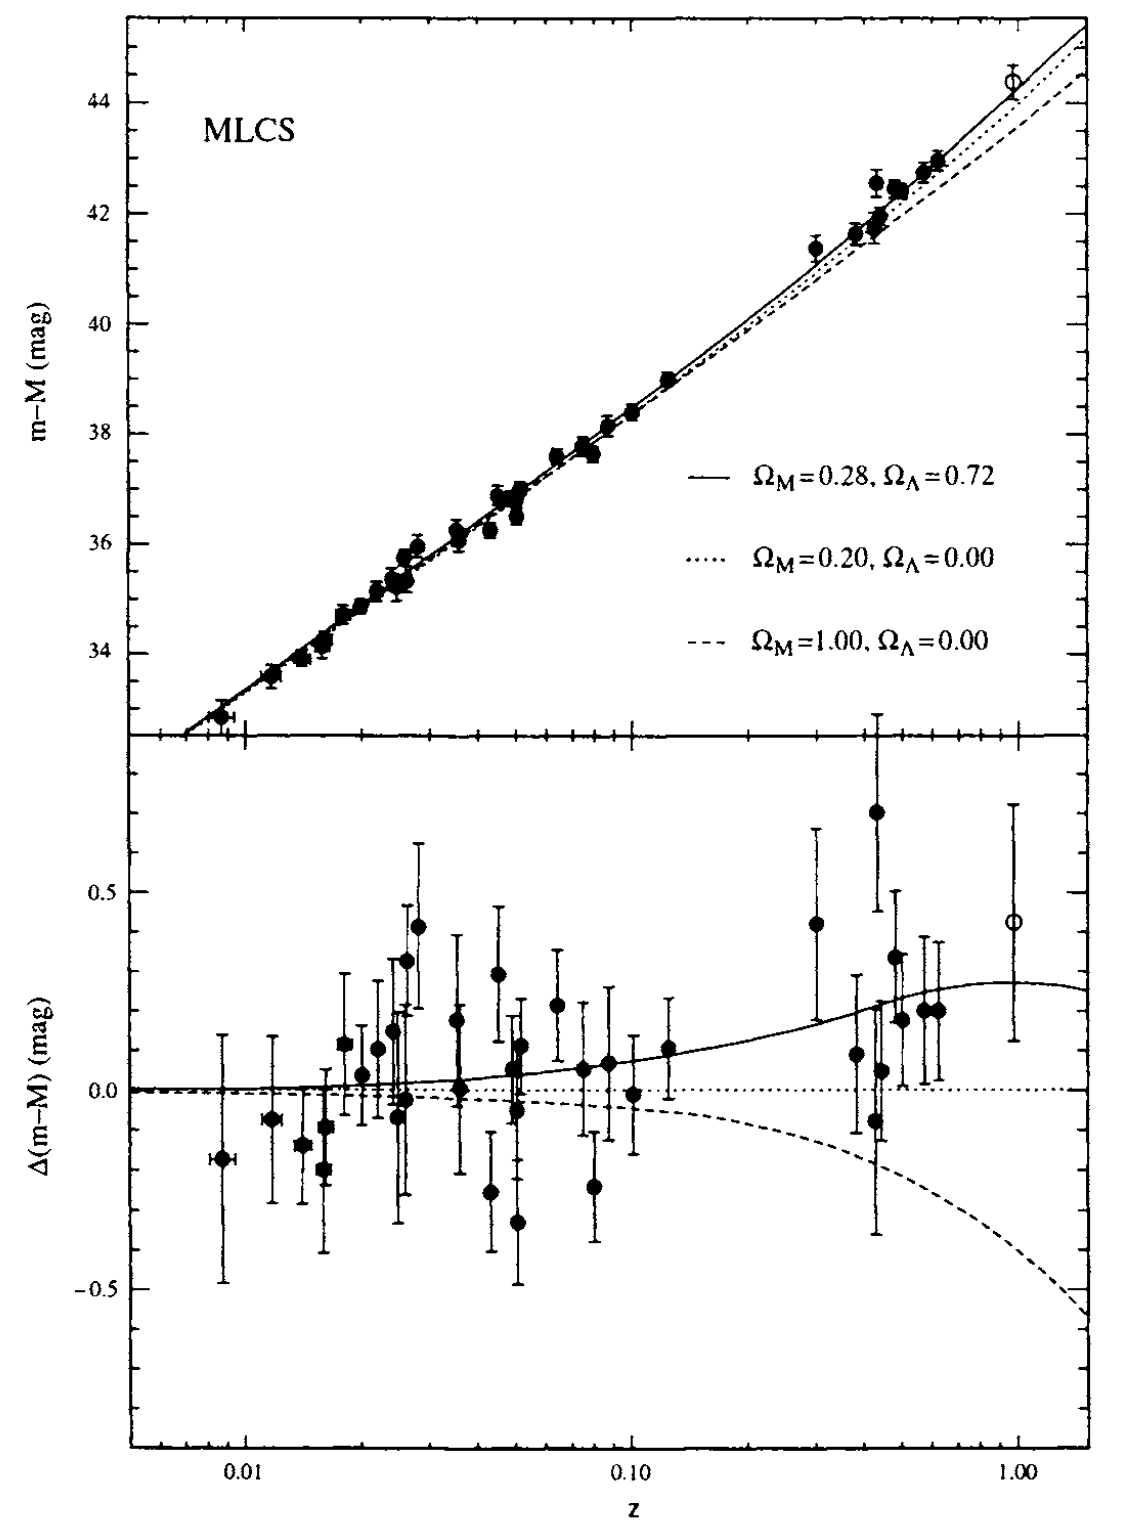
\includegraphics[width=10cm]{figures/cosmology/HubbleDiagram_modern.png}}
\end{figure}

\subsubsection{Additional context}

{\noindent}In recent years, the standard candle of choice among cosmologists has been Type Ia supernovae (SNe). A supernova may be loosely defined as an exploding star. Early in the history of supernova studies, when little was known about their underlying physics, supernovae were divided into two classes, on the basis of their spectra. Type I supernovae contain no hydrogen absorption lines in their spectra; Type II supernovae contain strong hydrogen absorption lines. Gradually, it was realized that all Type II supernovae are the same species of beast; they are massive stars ($M>8\,M_\odot$) whose cores collapse to form a black hole or neutron star when their nuclear fuel is exhausted. During the rapid collapse of the core, the outer layers of the star are thrown off into space. Type I supernovae are actually two separate species, which are called Type Ia and Type Ib. Type Ib supernovae, it is thought, are massive stars whose cores collapse after the hydrogen-rich outer layers of the star have been blown away in strong stellar winds. Thus, Type Ib and Type II supernovae are driven by very similar mechanisms -- their differences are superficial, in the most literal sense. Type Ia supernovae, however, are something completely different. They occur in close binary systems where one of the two stars in the system is a white dwarf; that is, a stellar remnant which is supported against gravity by electron degeneracy pressure. The transfer of mass from the companion star to the white dwarf eventually nudges the white dwarf over the Chandrasekhar limit of $1.4\,M_\odot$; this is the maximum mass at which the electron degeneracy pressure can support a white dwarf against its own self-gravity. When the Chandrasekhar limit is exceeded, the white dwarf starts to collapse until its increased density triggers a runaway nuclear fusion reaction. The entire white dwarf becomes a fusion bomb, blowing itself to smithereens; unlike Type II supernovae, Type Ia supernovae do not leave a condensed stellar remnant behind.

{\noindent}Within our Galaxy, Type Ia supernovae occur roughly once per century, on average. Although Type Ia supernovae are not frequent occurrences locally, they are extraordinarily luminous, and hence can be seen to large distances. The luminosity of an average Type Ia supernova, at peak brightness, is $L=4\times10^9\,\mathrm{L}_\odot$; that’s 100,000 times more luminous than even the brightest Cepheid. For a few days, a Type Ia supernova in a moderately bright galaxy can outshine all the other stars in the galaxy combined. Since moderately bright galaxies can be seen at $z\sim1$, this means that Type Ia supernovae can also be seen at $z\sim1$. Not only are Type Ia supernovae bright standard candles, they are also reasonably standardized standard candles. Consider Type Ia supernovae in the Virgo cluster. Although there’s only one Type Ia supernova per century in our own Galaxy, the total luminosity of the Virgo cluster is a few hundred times that of our Galaxy. Thus, every year you can expect a few type Ia supernovae to go off in the Virgo cluster. Several type Ia supernovae have been observed in the Virgo cluster in the recent past, and have been found to have similar fluxes at maximum brightness.

{\noindent}So far, Type Ia supernovae sound like ideal standard candles; very luminous and very standardized. There’s one complication, however. Observation of supernovae in galaxies whose distances have been well determined by Cepheids reveal that Type Ia supernovae do not have identical luminosities. Instead of all having $L = 4\times10^9\,\mathrm{L}_\odot$, their peak luminosities lie in the fairly broad range $L = 3\rightarrow5\times10^9\,\mathrm{L}_\odot$. However, it has also been noted that the peak luminosity of a Type Ia supernova is tightly correlated with the shape of its light curve. Type Ia supernovae with luminosities the shoot up rapidly and decline rapidly are less luminous than average at their peak; supernovae with luminosities which rise and fall in a more leisurely manner are more luminous than average at their peak. Thus, just as the period of a Cepheid tells you its luminosity, the rise and fall time of a Type Ia supernova tells you its peak luminosity.

{\noindent}Recently, two research teams, the ``Supernova Cosmology Project'' and the ``High-z Supernova Search Team'', have been conducting searches for supernovae in distant galaxies. They have used the observed light curves and redshifts of Type Ia supernovae to measure cosmological parameters. First, by observing Type Ia supernovae at $z\sim0.1$, the value of $H_0$ can be determined. The results of the different groups are in reasonable agreement with each other. If the distance to the Virgo cluster is pegged at $d_L = 15\,{\rm Mpc}$, as indicated by the Cepheid results, then the observed supernovae fluxes and redshifts are consistent with $H_0 = 70\pm7\,{\rm km\,s^{-1}\,Mpc^{-1}}$.

{\noindent}In addition, the supernova groups have been attempting to measure the acceleration (or deceleration) of the Universe by observing Type Ia supernovae at higher redshift. Before discussing these results, let's introduce the ``magnitude'' system used by astronomers to express fluxes and luminosities. The magnitude system, like much else in astronomy, has its roots in ancient Greece. The Greek astronomer Hipparchus, in the second century BC, divided the stars into six classes, according to their apparent brightness. The brightest stars were of ``first magnitude'', the faintest stars visible to the naked eye were of ``sixth magnitude'', and intermediate stars were ranked as second, third, fourth, and fifth magnitude. Long after the time of Hipparchus, it was realized that the response of the human eye is roughly logarithmic, and that stars of the first magnitude have fluxes (at visible wavelengths) about 100 times greater than stars of the sixth magnitude. On the basis of this realization, the magnitude system was placed on a more rigorous mathematical basis.

{\noindent}Nowadays, the bolometric apparent magnitude of a light source is defined in terms of the source’s \textbf{bolometric flux} as

\begin{align*}
    m \equiv -2.5\log_{10}\left(\frac{F}{F_0}\right) ~ [{\rm mag}],
\end{align*}

{\noindent}where the reference flux $F_0$ is set at the value $F_0 = 2.53\times10^{-8}\,[{\rm W\,m^{-2}}]$. Thanks to the negative sign in the definition, a small value of $m$ corresponds to a large flux $F$. For instance, the flux of sunlight at the Earth’s location is $F = 1367\,[{\rm W\,m^{-2}}]$; the Sun thus has a bolometric apparent magnitude of $m = −26.8$. The choice of reference flux $F_0$ constitutes a tip of the hat to Hipparchus, since for stars visible to the naked eye it typically yields $0 < m < 6$.

{\noindent}The bolometric absolute magnitude of a light source is defined as the apparent magnitude that it would have if it were at a luminosity distance of $d_L = 10\,{\rm pc}$. Thus, a light source with luminosity L has a bolometric \textbf{absolute magnitude} of

\begin{align*}
    M \equiv -2.5\log_{10}\left(\frac{L}{L_0}\right) ~ [{\rm mag}],
\end{align*}

{\noindent}where the reference luminosity is $L_0=78.7\,\mathrm{L}_\odot$, since that is the luminosity of an object which produces a flux $F_0 = 2.53\times10^{-8}\,[{\rm W\,m^{-2}}]$ when viewed from a distance of $10\,{\rm pc}$. The bolometric absolute magnitude of the Sun is thus $M = 4.74$. Although the system of apparent and absolute magnitudes seems strange to the uninitiated, the apparent magnitude is really nothing more than a logarithmic measure of the flux, and the absolute magnitude is a logarithmic measure of the luminosity.

{\noindent}Given the definitions of apparent and absolute magnitude, the relation between an object’s apparent magnitude and its absolute magnitude can be written in the form

\begin{align*}
    M = m -5\log_{10}\left(\frac{d_L}{10\,{\rm pc}}\right) ~ [{\rm mag}],
\end{align*}

{\noindent}where $d_L$ is the luminosity distance to the light source. If the luminosity distance is given in units of megaparsecs, this relation becomes

\begin{align*}
    M = m -5\log_{10}\left(\frac{d_L}{1\,{\rm Mpc}}\right)-25 ~ [{\rm mag}].
\end{align*}

{\noindent}Since astronomers frequently quote fluxes and luminosities in terms of apparent and absolute magnitudes, they find it convenient to quote luminosity distances in terms of the distance modulus to a light source. The \textbf{distance modulus} is defined as $m-M$, and is related to the luminosity distance by the relation

\begin{align*}
    m - M = 5\log_{10}\left(\frac{d_L}{1\,{\rm Mpc}}\right)-25 ~ [{\rm mag}].
\end{align*}

{\noindent}The distance modulus of the Large Magellanic Cloud (LMC), for instance, at $d_L = 0.05\,{\rm Mpc}$, is $m - M = 18.5$. The distance modulus of the Virgo cluster, at $d_L = 15\,{\rm Mpc}$, is $m - M = 30.9$. 

{\noindent}Unfortunately, the current proper distance to a Type 1a supernova is not a measurable property. If you tried to measure the distance with a tape measure, for instance, the distance would be continuously increasing as you extended the tape. To measure the proper distance at time $t_0$, you would need a tape measure which could be extended with infinite speed; alternatively, you would need to stop the expansion of the Universe at its current scale factor while you measured the distance at your leisure. Neither of these alternatives is physically possible.

{\noindent}Since cosmology is ultimately based on observations, if we want to find the distance to a galaxy, we need some way of computing a distance from that galaxy’s observed properties. For objects at cosmological distances, we can measure the flux of light, $F$, from the object. The complete flux, integrated over all wavelengths of light, is called the bolometric flux. (A bolometer is an extremely sensitive thermometer capable of detecting electromagnetic radiation over a wide range of wavelengths; it was invented in 1881 by the astronomer Samuel Langley, who used it to measure solar radiation.) More frequently, given the difficulties of measuring the true bolometric flux, the flux over a limited range of wavelengths is measured. If the light from the object has emission or absorption lines, we can measure the redshift, $z$.

{\noindent}Since Type 1a supernovae are standard candles in the sense that their luminosities can be measured, then you can use its measured flux $F$ to define a function called the \textbf{luminosity distance}:

\begin{align*}
    d_L \equiv \sqrt{\frac{L}{4\pi F}} ~ [{\rm Mpc}].
\end{align*}

{\noindent}The function $d_L$ is called a ``distance'' because its dimensionality is that of a distance, and because it is what the proper distance to the standard candle would be if the Universe were static and Euclidean. In a static Euclidean Universe, the propagation of light follows the inverse square law $F = L/(4\pi d^2)$.

{\noindent}Suppose, though, that you are in a Universe described by a \textbf{Robertson-Walker metric}:

\begin{align*}
    \mathrm{d}s^2 = - c^2\mathrm{d}t^2 + a(t)^2(\mathrm{d}r^2 + S_\kappa(r)^2\mathrm{d}\Omega^2),
\end{align*}

{\noindent}with 

\begin{align*}
    S_\kappa(r) =
    \left\{
    \begin{aligned}
    R\sin(r/R), ~~~~~& (\kappa = +1) \\
              r,~~~~~& (\kappa = 0) \\
    R\sinh(r/R),~~~~~& (\kappa = -1)
    \end{aligned}
    \right.
    .
\end{align*}

{\noindent}You are at the origin. At the present moment $t = t_0$, you see light that was emitted by a standard candle at comoving coordinate location $(r,\theta,\phi)$ at a time $t_e$. The photons which were emitted at time $t_e$ are, at the present moment, spread over a sphere of proper radius $d_p(t_0) = r$ and proper surface area $A_p(t_0)$. If space is flat $(\kappa=0)$, then the proper area of the sphere is given by the Euclidean relation $A_p(t_0) = 4\pi d_p(t_0)^2 = 4\pi r^2$. More generally, however,

\begin{align*}
    A_p(t_0) = 4\pi S_\kappa(r)^2 ~ [{\rm Mpc^2}].
\end{align*}

{\noindent}When space is positively curved, $A_p(t_0) < 4\pi r^2$, and the photons are spread over a smaller area than they would be in flat space. When space is negatively curved, $A_p(t_0) > 4\pi r^2$, and photons are spread over a larger area than they would be in flat space.

{\noindent}In addition to these geometric effects, which would apply even in a static Universe, the expansion of the Universe causes the observed flux of light from a standard candle of redshift $z$ to be decreased by a factor of $(1+z)^{−2}$. First, the expansion of the Universe causes the energy of each photon from the standard candle to decrease. If a photon starts with an emitted energy $E = hc/λ$ when the scale factor is $a(t)$, by the time we observe it when the scale factor is A$a(t_0) = 1$, the wavelength will have grown to

\begin{align*}
    \lambda_0 = \frac{1}{a(t)}\lambda = (1+z)\lambda ~ [{\rm m}],
\end{align*}

{\noindent}and the energy will have fallen to

\begin{align*}
    E_0 = E(1+z)^{-1} ~ [{\rm eV}].
\end{align*}

{\noindent}Second, thanks to the expansion of the Universe, the time between photon detections will be greater. If two photons are emitted in the same direction separated by a time interval $\delta t$, the proper distance between them will initially be $c\delta t$; by the time we detect the photons at time $t_0$, the proper distance between them will be stretched to $c\delta t(1 + z)$, and we will detect them separated by a time interval $\delta t_0 = \delta t(1 + z)$.

{\noindent}The net result is that in an expanding, spatially curved Universe, the relation between the observed flux $F$ and the luminosity $L$ of a distant light source is

\begin{align*}
    F = \frac{L}{4\pi S_\kappa(r)^2(1+z)^2} ~ [{\rm W\,m^{-2}}],
\end{align*}

{\noindent}and the luminosity distance is

\begin{align*}
    d_L = S_\kappa(r)(1+z) ~ [{\rm Mpc}].
\end{align*}

{\noindent}The available evidence indicates that our Universe is nearly flat, with a radius of curvature $R_0$ which is larger than the current horizon distance $d_\mathrm{hor}(t_0)$. Objects with finite redshift are at proper distances smaller than the horizon distance, and hence smaller than the radius of curvature. Thus, it is safe to make the approximation $r \ll R_0$, implying $S\kappa(r) \approx r$. With our assumption that space is very close to being flat, the relation between the luminosity distance and the current proper distance becomes very simple:

\begin{align*}
    d_L(\kappa=0) = r(1+z) = d_p(t_0)(1+z) ~ [{\rm Mpc}].
\end{align*}

{\noindent}Thus, even if space is perfectly flat, if you estimate the distance to a standard candle by using a naive inverse square law, you will overestimate the actual proper distance by a factor $(1+z)$.

\begin{figure}[h]
    \floatbox[{\capbeside\thisfloatsetup{capbesideposition={right,top},capbesidewidth=4cm}}]{figure}[\FBwidth]
    {\caption{\footnotesize{The luminosity distance of a standard candle with observed redshift $z$. The bold solid line gives the result for the Benchmark Model, the dot-dash line for a flat, $\Lambda$-only Universe, and the dotted line for a flat, matter-only Universe. Figure taken from Ryden (2006).}}
    \label{fig:luminositydistance}}
    {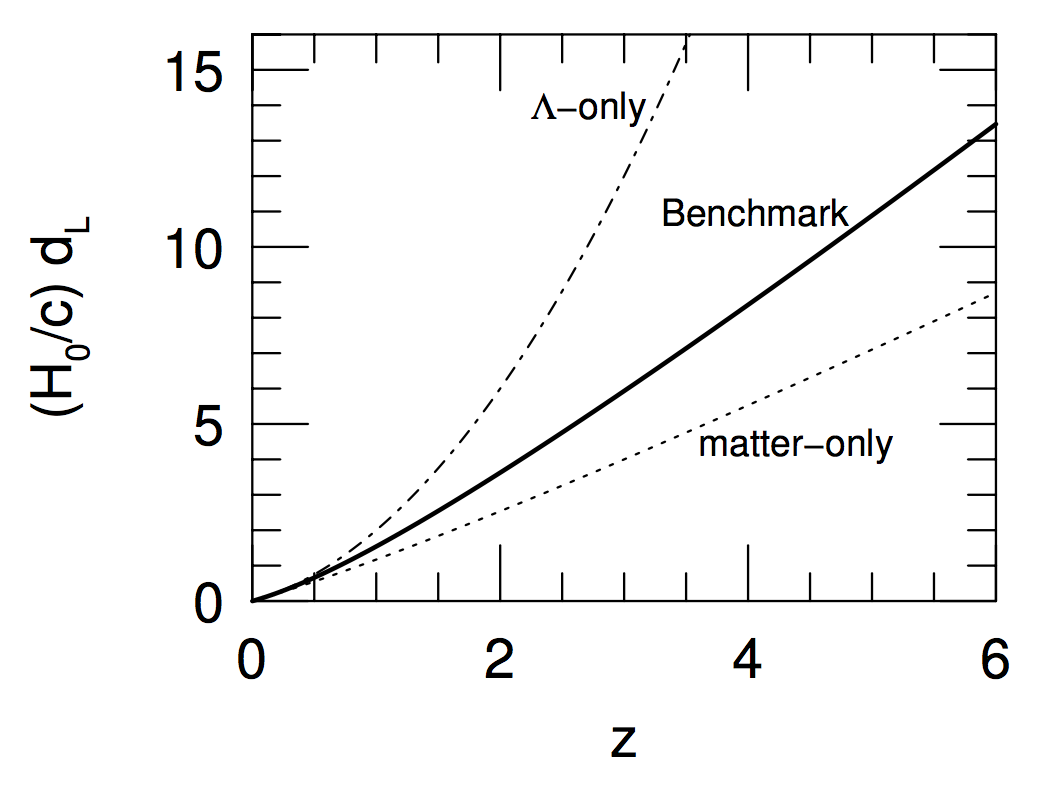
\includegraphics[width=10cm]{figures/cosmology/LuminosityDistance.png}}
\end{figure}

{\noindent}Figure \ref{fig:luminositydistance} shows the luminosity distance $d_L$ as a function of redshift $z$ for the Benchmark Model, and for two other flat Universes, one dominated by matter and one dominated by a cosmological constant $\Lambda$. When $z\ll1$, the current proper distance may be approximated as

\begin{align*}
    d_p(t_0) \approx \frac{c}{H_0}z \left(1-\frac{1+q_0}{2}z\right) ~ [{\rm Mpc}].
\end{align*}

{\noindent}In a Universe which is nearly flat, the luminosity distance may thus be approximated as

\begin{align*}
    d_L &\approx \frac{c}{H_0}z \left(1-\frac{1+q_0}{2}z\right)(1+z) \\
        & \approx \frac{c}{H_0}z \left(1+\frac{1-q_0}{2}z\right).
\end{align*}

{\noindent}Note that in the limit $z\rightarrow0$,

\begin{align*}
    d_p(t_0) \approx d_L \approx \frac{c}{H_0}z ~ [{\rm Mpc}].
\end{align*}

{\noindent}In a Universe described by the Robertson-Walker metric, the luminosity distance is a good approximation to the current proper distance for objects with small redshifts.

{\noindent}Substituting the luminositxy distance approximation into the expression for the distance modulus gives us the relation between distance modulus and redshift:

\begin{align*}
    m - M \approx 43.17 - 5\log_{10} \left(\frac{H_0}{70\,{\rm km\,s^{-1}\,Mpc}}\right) + 5\log_{10}z + 1.086(1-q_0)z ~ [{\rm mag}].
\end{align*}

{\noindent}For a population of standard candles with known luminosity $L$ (and hence of known bolometric absolute magnitude $M$), you measure the flux $F$ (or equivalently, the bolometric apparent magnitude $m$) and the redshift $z$. In the limit $z\rightarrow0$, a plot of $m-M$ versus $\log_{10}(z)$ gives a straight line whose amplitude at a given value of $z$ tells you the value of $H_0$. At slightly larger values of $z$, the deviation of the plot from a straight line tells you the value of $q_0$. At a given value of $z$, an accelerating Universe (with $q_0<0$) yields standard candles with a smaller flux than would a decelerating Universe (with $q_0>0$).

\begin{figure}[h]
    \floatbox[{\capbeside\thisfloatsetup{capbesideposition={right,top},capbesidewidth=4cm}}]{figure}[\FBwidth]
    {\caption{\footnotesize{Distance modulus versus redshift for Type Ia supernovae from the Supernova Cosmology Project (Perlmutter et al. 1999, ApJ, 517, 565) and the High-z Supernova Search Team (Riess et al. 1998, AJ, 116, 1009). The bottom panel shows the difference between the data and the predictions of a negatively curved $\Omega_{m,0}=0.3$ model (from Riess 2000, PASP, 112, 1284). Figure taken from Ryden (2006).}}
    \label{fig:distancemodulus}}
    {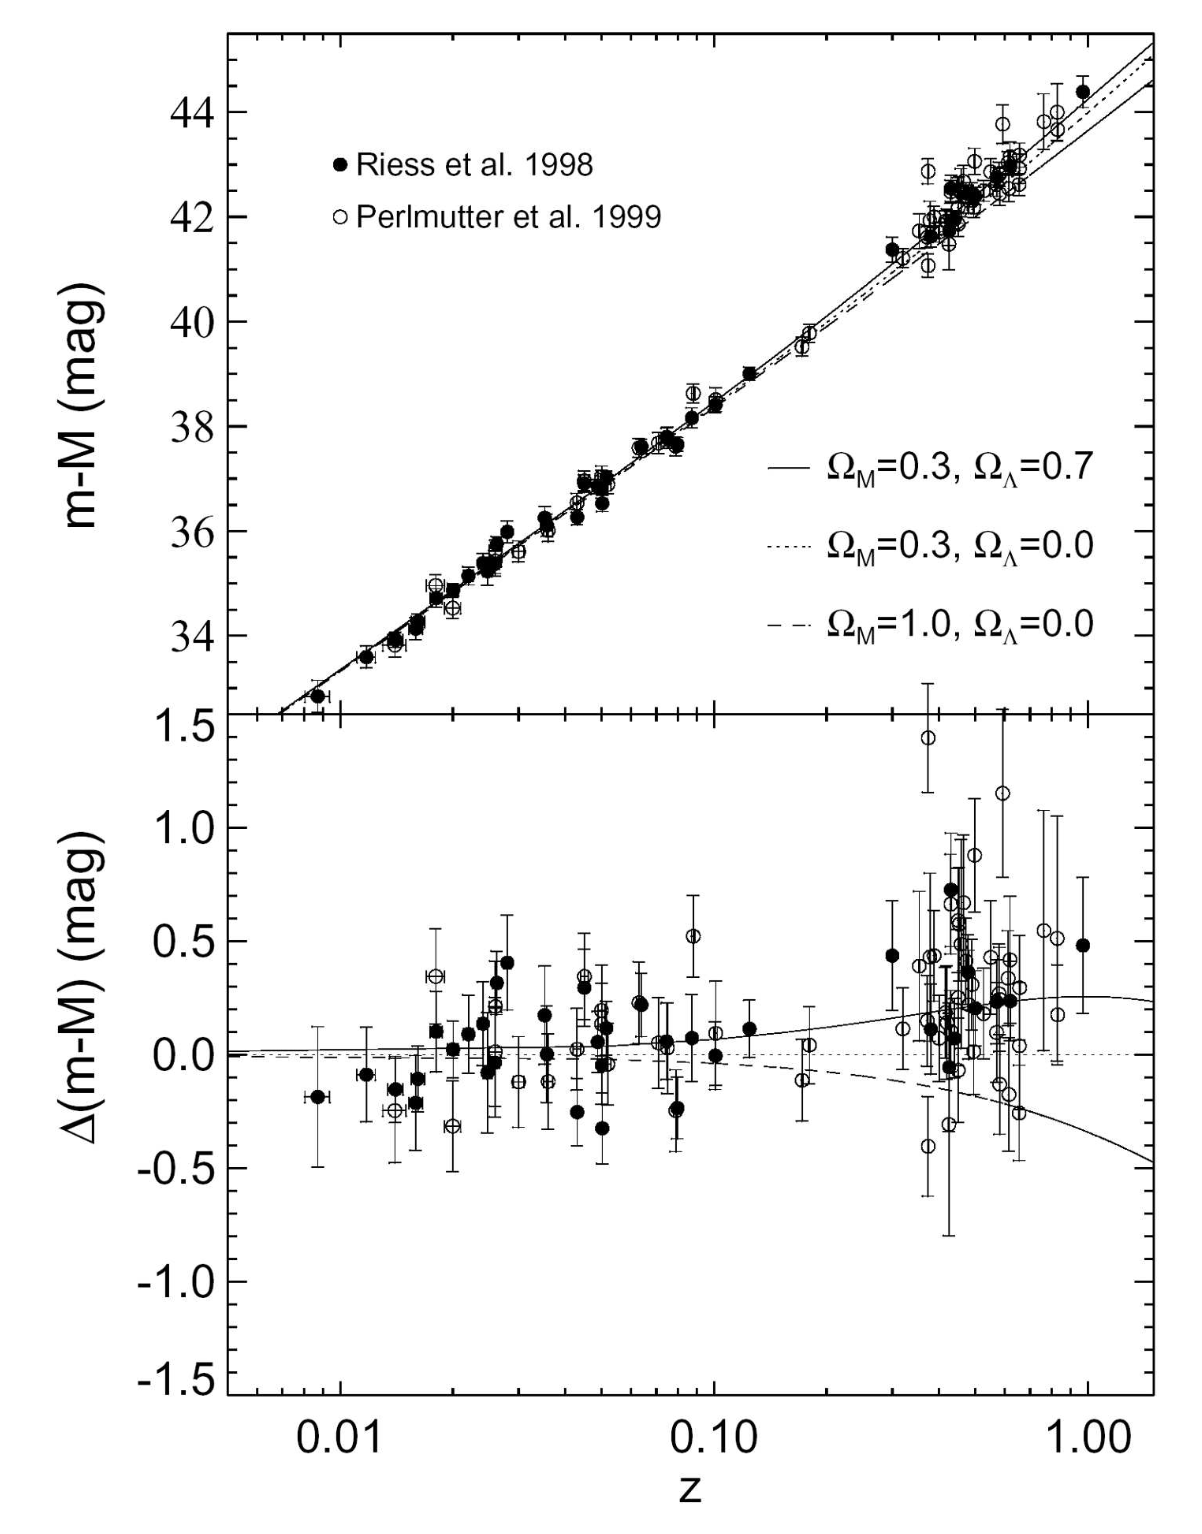
\includegraphics[width=11cm]{figures/cosmology/DistanceModulus.png}}
\end{figure}

{\noindent}The upper panel of Figure \ref{fig:distancemodulus} shows the plot of distance modulus versus redshift for the combined supernova samples of the High-z Supernova Search Team (given by the filled circles) and the Supernova Cosmology Project (given by the open circles). The observational results are compared to the expected results for three model Universes. One Universe is flat, and contains nothing but matter $(\Omega_{m,0}=1, q_0=0.5)$. The second is negatively curved, and contains nothing but matter $(\Omega_{m,0}=0.3, q_0=0.15)$. The third is flat, and contains both matter and a cosmological constant $(\Omega_{m,0}=0.3, \Omega_{\Lambda,0}=0.7, q_0=−0.55).$ The data are best fitted by the third of the models -- which is, in fact, our Benchmark Model. The bottom panel of Figure \ref{fig:distancemodulus} shows this result more clearly. It shows the difference between the data and the predictions of the negatively curved, matter-only model. The conclusion that the Universe is accelerating derives from the observation that the supernovae seen at $z \sim 0.5$ are, on average, about $0.25\,{\rm mag}$ fainter than they would in a decelerating Universe with $\Omega_{m,0}=0.3$ and no cosmological constant.
 
\begin{figure}[h]
    \floatbox[{\capbeside\thisfloatsetup{capbesideposition={right,top},capbesidewidth=4cm}}]{figure}[\FBwidth]
    {\caption{\footnotesize{The values of $\Omega_{m,0}$ (horizontal axis) and $\Omega_{\Lambda,0}$ (vertical axis) which best fit the data shown in Figure \ref{fig:distancemodulus}. The solid ovals show the best-fitting values for the High-z Supernova Search Team data; the dotted ovals show the best-fitting values for the Supernova Cosmology Project data (from Riess 2000, PASP, 112, 1284) Figure taken from Ryden (2006).}}
    \label{fig:omegamodel}}
    {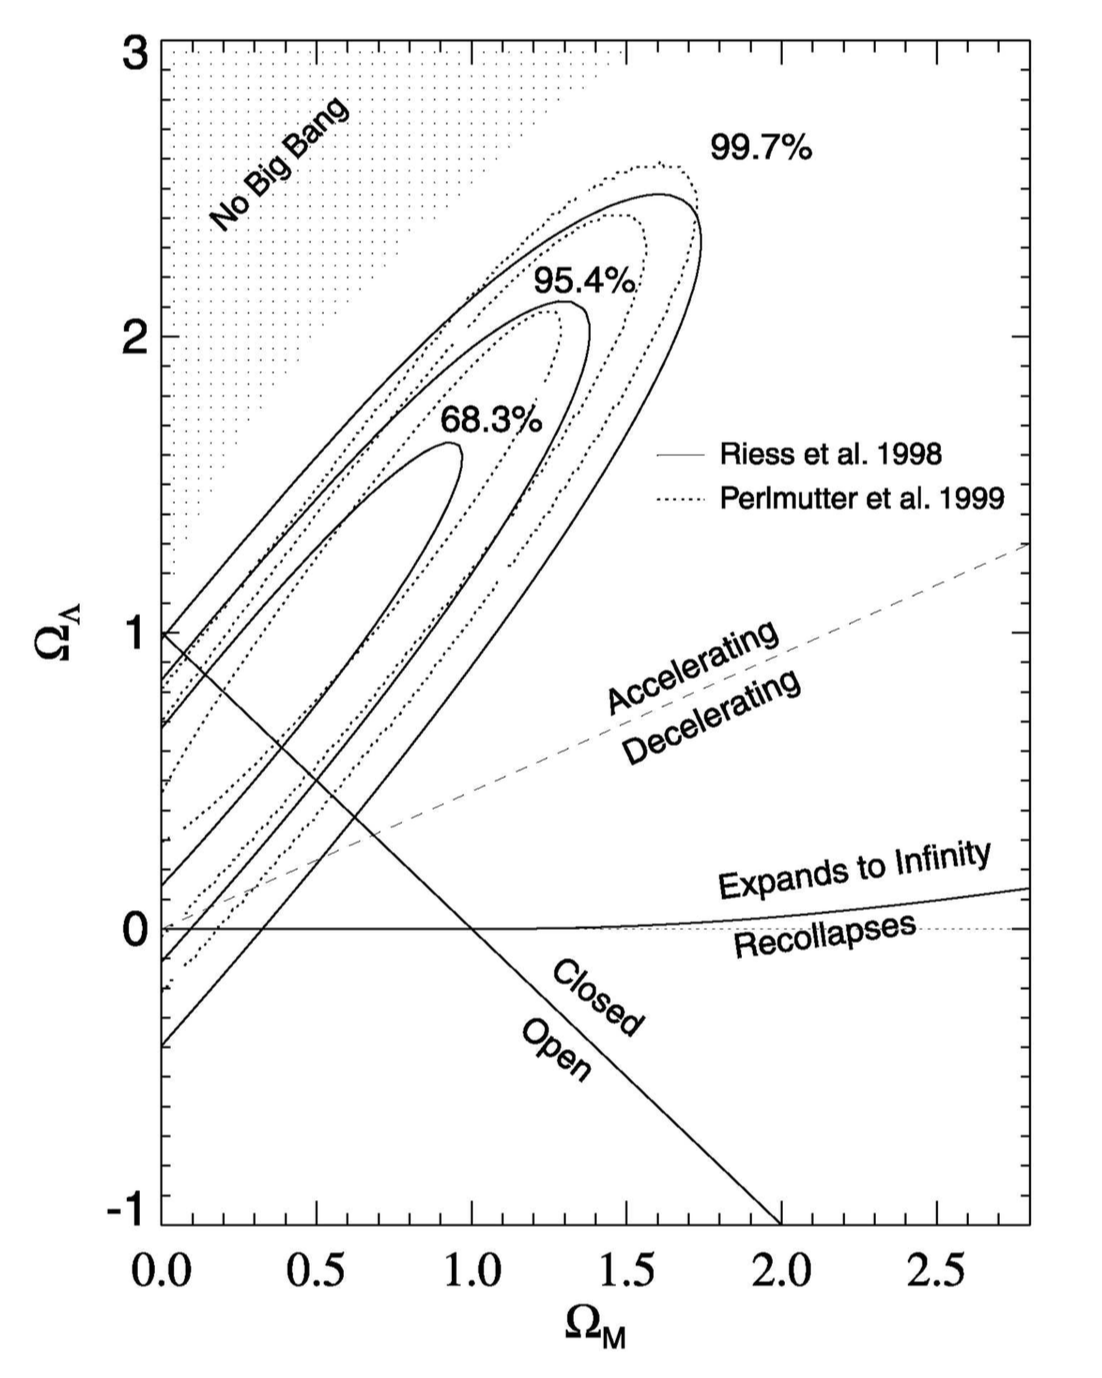
\includegraphics[width=10cm]{figures/cosmology/OmegaModel.png}}
\end{figure}

{\noindent}The supernova data extend out to $z\sim1$; this is beyond the range where an expansion in terms of $H_0$ and $q_0$ is adequate to describe the scale factor $a(t)$. Thus, the two supernova teams customarily describe their results in terms of a model Universe which contains both matter and a cosmological constant. After choosing values of $\Omega_{m,0}$ and $\Omega_{\Lambda,0}$, they compute the expected relation between $m-M$ and $z$, and compare it to the observed data. The results of fitting these model Universes are given in Figure \ref{fig:omegamodel}. The ovals drawn on Figure \ref{fig:omegamodel} enclose those values of $\Omega{m,0}$ and $\Omega_{\Lambda,0}$ which give the best fit to the supernova data. The results of the two teams (the solid ovals and dotted ovals) give very similar results. Three concentric ovals are shown for each team’s result; they correspond to $1\sigma$, $2\sigma$, and $3\sigma$ confidence intervals, with the inner oval representing the highest probability. The best fitting models lie along the line $0.8\Omega{m,0}-0.6\Omega_{\Lambda,0}\approx-0.2.$ Note that decelerating Universes (with $q_0>0$) can be strongly excluded by the data, as can Big Crunch Universes (labeled `Recollapses' in Figure \ref{fig:omegamodel}), and Big Bounce Universes (labeled `No Big Bang' in Figure \ref{fig:omegamodel}). The supernova data are consistent with negative curvature (labeled `Open' in Figure \ref{fig:omegamodel}), positive curvature (labeled `Closed' in Figure \ref{fig:omegamodel}), or with a Universe which is spatially flat.

{\noindent}The results of the supernova teams made headlines when they were first announced; the discovery of the accelerating Universe was named by Science magazine as the `Scientific Breakthrough of the Year' for 1998. It is prudent to remember, however, that all the hoopla about the accelerating Universe is based on the observation that Type Ia supernova at $z\sim0.5$ and beyond have somewhat lower fluxes (by about 25\%) than they would have in a decelerating Universe. There are other reasons why their fluxes might be low. For instance, if Type Ia supernovae were intrinsically less luminous at $z\sim0.5$ than at $z\sim0$, that could explain their low fluxes. (If a typical supernova at $z\sim0.5$ had $L=3\times10^9\,\mathrm{L}_\odot$ rather than $L=4\times10^9\,\mathrm{L}_\odot$, that would explain their observed dimness, without the need to invoke a cosmological constant. Conversely, if the typical supernova at $z\sim0.5$ had $L=5\times10^9\,\mathrm{L}_\odot$ rather than $L=4\times10^9\,\mathrm{L}_\odot$, that would require an even larger cosmological constant to explain their observed dimness.) However, the other properties of Type Ia supernovae, such as their spectra, don’t seem to evolve with time, so why should their luminosity? Perhaps the fluxes of supernovae at $z\sim0.5$ are low because some of their light is scattered or absorbed by intervening dust. However, dust tends to scatter some wavelengths of light more than others. This would change the shape of the spectrum of distant Type Ia supernovae, but no dependence of spectral shape on redshift is observed.

{\noindent}In sum, the supernova results of Figure \ref{fig:omegamodel} provide persuasive evidence for a nearly flat accelerating Universe with $\Omega_{m,0}\approx0.3$ and $\Omega_{\Lambda,0}\approx0.7$.

\subsubsection{Follow-up Questions}

\begin{itemize}
    \item What are Type Ia supernovae (i.e., what is physically happening)?
    \item Can Type Ia constrain all cosmological parameters?
    \item What are some sources of error? (Maximum luminosity is not perfectly consistent but the light curve can be used to calibrate this due to their tight correlation.)
    \item How do we know that redshift can be used as a measurement of distance? (Wanted to hear about Hubble's Law.)
    \item Can other types of supernovae be used as standard candles? Why or why not?
\end{itemize}

% --------------------------------------------------------------
%
%                           8. 
%
% --------------------------------------------------------------

\newpage
\subsection{Question 8}

Describe two methods, other than Type Ia supernovae, by which the cosmological parameters can be determined by astronomical observations.

\subsubsection{Short answer}

\textbf{CMB Angular Power Spectrum}: Comparisons of the relative strengths of the first few peaks can inform you about $\Omega_m$ and $\Omega_\Lambda$ since these are the components that caused the oscillations. In addition to this, the smallest multipole moments (i.e., the largest of scales) in the power spectrum can tell you about the modes that were never affected by the sound horizon and should tell you about inflation and the initial conditions that remain unperturbed. In contrast, the largest multipole moments (i.e., the smallest scales) in the power spectrum can tell you about Silk damping.

{\noindent}\textbf{BAOs}: The peaks in the CMB angular power spectrum are the result of compressions and expansions of the baryonic acoustic oscillations: the first and second peaks being the first compression and first decompression, respectively, etc. Given that the first compression happened on scales of the sound horizon at the time of last scattering, the first peak in the CMB angular power spectrum should tell you at what that scale was. This scale (i.e., the sound horizon) can be compared to what would be expected for a flat Universe -- if it is smaller, the Universe is open whereas if it is larger, the Universe is closed (if they're equal, the Universe is of course flat).

\subsubsection{Additional context}

\textbf{CMB Angular Power Spectrum}: The cosmic microwave background consists of photons that last interacted with matter at $z\sim1,100$. Since the Universe must already have been inhomogeneous at this time, in order for the structures present in the current Universe to be able to form, it is expected that these spatial inhomogeneities are visible as a (small) anisotropy of the CMB: \textit{the angular distribution of the CMB temperature reflects the matter inhomogeneities at the redshift of decoupling of radiation and matter}. The CMB anisotropies reflect the conditions in the Universe at the epoch of recombination, thus at $z\sim1,100$. Temperature fluctuations originating at this time are called \textbf{primary anisotropies}. Later, as the CMB photons propagate through the Universe, they may experience a number of distortions along their way which, again, may change their temperature distribution on the sky. These effects then lead to \textbf{secondary anisotropies}.

{\noindent}Of the primary anisotropies (which directly pertain to inhomogeneities at the time of last scattering) the most basic mechanisms can be divided into those which occur on scales larger than the horizon size at recombination, i.e., which can not have been affected by physical interactions up to the time of last scattering, and those on smaller scales. The effects on superhorizon scales are the following:

\begin{itemize}
    \item \textbf{Sachs-Wolfe effect}: Inhomogeneities in the gravitational potential cause photons which originate in regions of higher density to climb out of a potential well. As a result of this, they lose energy and are redshifted (\textbf{gravitational redshift}). This effect is partly compensated for by the fact that, besides the gravitational redshift, a gravitational time delay also occurs: a photon that originates in an overdense region will be scattered at a slightly earlier time, and thus at a slightly higher temperature of the Universe, compared to a photon from a region of average density. Both effects always occur side by side. This results in photons that are cooler in baryon overdensities. (This is the dominant mechanism of primary anisotropies at superhorizon scales.)
    \item \textbf{Peculiar velocities}: The electrons that scatter the CMB photons for the last time do not follow exactly the Hubble expansion, but have an additional velocity that is closely linked to the density fluctuations. This results in a Doppler effect: if photons are scattered by gas receding from us with a speed larger than that corresponding to the Hubble expansion, these photons experience an additional redshift which reduces the temperature measured in that direction.
    \item \textbf{Enhanced baryon density}: The distribution of baryons follows that of the dark matter, so that in regions of a higher dark matter density, the baryon density is also enhanced. This leads to an increased temperature of the baryons in overdense regions.
\end{itemize}

{\noindent}These three effects are relevant on scales larger than the (sound) horizon scale at the epoch of recombination. Obviously, they are closely coupled to each other. In particular, on scales $>r_\mathrm{H,com}(z_\mathrm{rec})$, the first two effects can partially compensate each other, though the Sachs-Wolfe effect is the dominant one at superhorizon scales. Inside the (sound) horizon, two other effects dominate the primary anisotropy signal:

\begin{enumerate}
    \item \textbf{Baryon acoustic oscillations}: On subhorizon scales, the pressure of the baryon-photon fluid is effective because, prior to recombination, these two components had been closely coupled by Compton scattering. This leads to sound waves in the baryon-photon fluid, called the baryonic acoustic oscillations (BAOs). In the density peaks of these sound waves, the baryon-photon fluid is adiabatically compressed and thus hotter than the average. The CMB sky yields a two-dimensional cut through this three-dimensional density (and temperature) field of these sound waves, and thus reflect these fluctuations, yielding temperature anisotropies with characteristic length (or angular) scales. (More on this later.)
    \item \textbf{Silk damping}: The coupling of baryons and photons is not perfect since, owing to the finite mean free path of photons, the two components are decoupled on small spatial scales. This implies that on small length-scales, the temperature fluctuations can be smeared out by the diffusion of photons. This process is known as \textbf{Silk damping}, and it implies that on angular scales below about $\sim50'$, only very small primary fluctuations exist.
\end{enumerate}

{\noindent}\textbf{BAOs}: On subhorizon scales, the pressure of the baryon-photon fluid is effective because, prior to recombination, these two components had been closely coupled by Compton scattering. This leads to sound waves in the baryon-photon fluid, called the baryonic acoustic oscillations (BAOs). In the density peaks of these sound waves, the baryon-photon fluid is adiabatically compressed and thus hotter than the average. The CMB sky yields a two-dimensional cut through this three-dimensional density (and temperature) field of these sound waves, and thus reflect these fluctuations, yielding temperature anisotropies with characteristic length (or angular) scales. The length-scale of the resulting density perturbation is given by the sound horizon at recombination; it depends only on the baryon-to-photon and the matter-to-radiation density ratios. The former is proportional to $\Omega_bh^2$ and is determined, e.g., from BBN; the latter is proportional to $\Omega_mh^2$ which is well determined from measurements of the CMB. Together, one finds that the acoustic scale has a comoving value of $r_s\approx150\,{\rm Mpc}$.

{\noindent}We expect that these frozen sound waves of the baryons leave an imprint on the overall matter correlation function, best seen in Figure \ref{fig:perturbationevolution}. This unique feature in the correlation function, if it can be detected in the galaxy correlation function, would provide a well-defined `standard rod' in the observable Universe. Since we can observe only angular scales on the sky, the relation between the (comoving) length of the standard rod and the associated angular scale provides a measure of distance. Therefore, a measurement of the baryonic acoustic oscillations (BAOs) in the correlation of galaxies at a given redshift $z$ can be used to determine the (comoving) angular diameter distance $d_A(z)$ --  which depends on the density parameters $\Omega_m$ and $\Omega_\Lambda$.

{\noindent}In fact, the three-dimensional correlation function does not only depend on the transverse length scale which is related to the angular scale via the angular-diameter distance, but also on the separation of galaxies along the line-of-sight. The comoving distance interval corresponding to a redshift interval $\Delta z$ is given by $\Delta x=c\Delta z/H(z)$. Since there are two transversal dimensions, and one along the line-of-sight, the distance measure that is determined best from BAOs is the geometric mean

\begin{align*}
    D(z) = \left(d_A^2(z)\frac{cz}{H(z)}\right)^{1/3}.
\end{align*}

{\noindent}The large redshift surveys 2dFGRS and SDSS allowed the first detection of these BAOs in the galaxy distribution in 2005. Figure \ref{fig:correlationfunction} shows the discovery of BAOs from the SDSS, where a clear feature in the galaxy correlation function is seen at the expected length scale. The mean redshift of the galaxies from which the correlation function was determined is $z\sim0.35$; thus, this measurement yields an estimate of the angular diameter distance to that redshift, with about a 5\% accuracy. In particular, we point out that the sound horizon at recombination is visible in the current Universe!

\begin{figure}[t]
    \floatbox[{\capbeside\thisfloatsetup{capbesideposition={right,top},capbesidewidth=4cm}}]{figure}[\FBwidth]
    {\caption{\footnotesize{The correlation function of galaxies, as observed in the SDSS, shows a clear indication of a secondary peak on a comoving scale of about $100h^{-1}\,{\rm Mpc}\sim150\,{\rm Mpc}$. Curves show models with slightly different density parameter $\Omega_mh^2 = 0.12; 0.13; 0.14$, with fixed baryon density of $\Omega_bh^2=0.024$. The lowest, smooth curve is a  CDM model without baryons which thus shows no features due to baryonic oscillations. Source: D. Eisenstein et al. 2005, Detection of the Baryon Acoustic Peak in the Large-Scale Correlation Function of SDSS Luminous Red Galaxies, ApJ 633, 560, p. 563, Fig. 2. Figure taken from Schneider (2006).}}
    \label{fig:correlationfunction}}
    {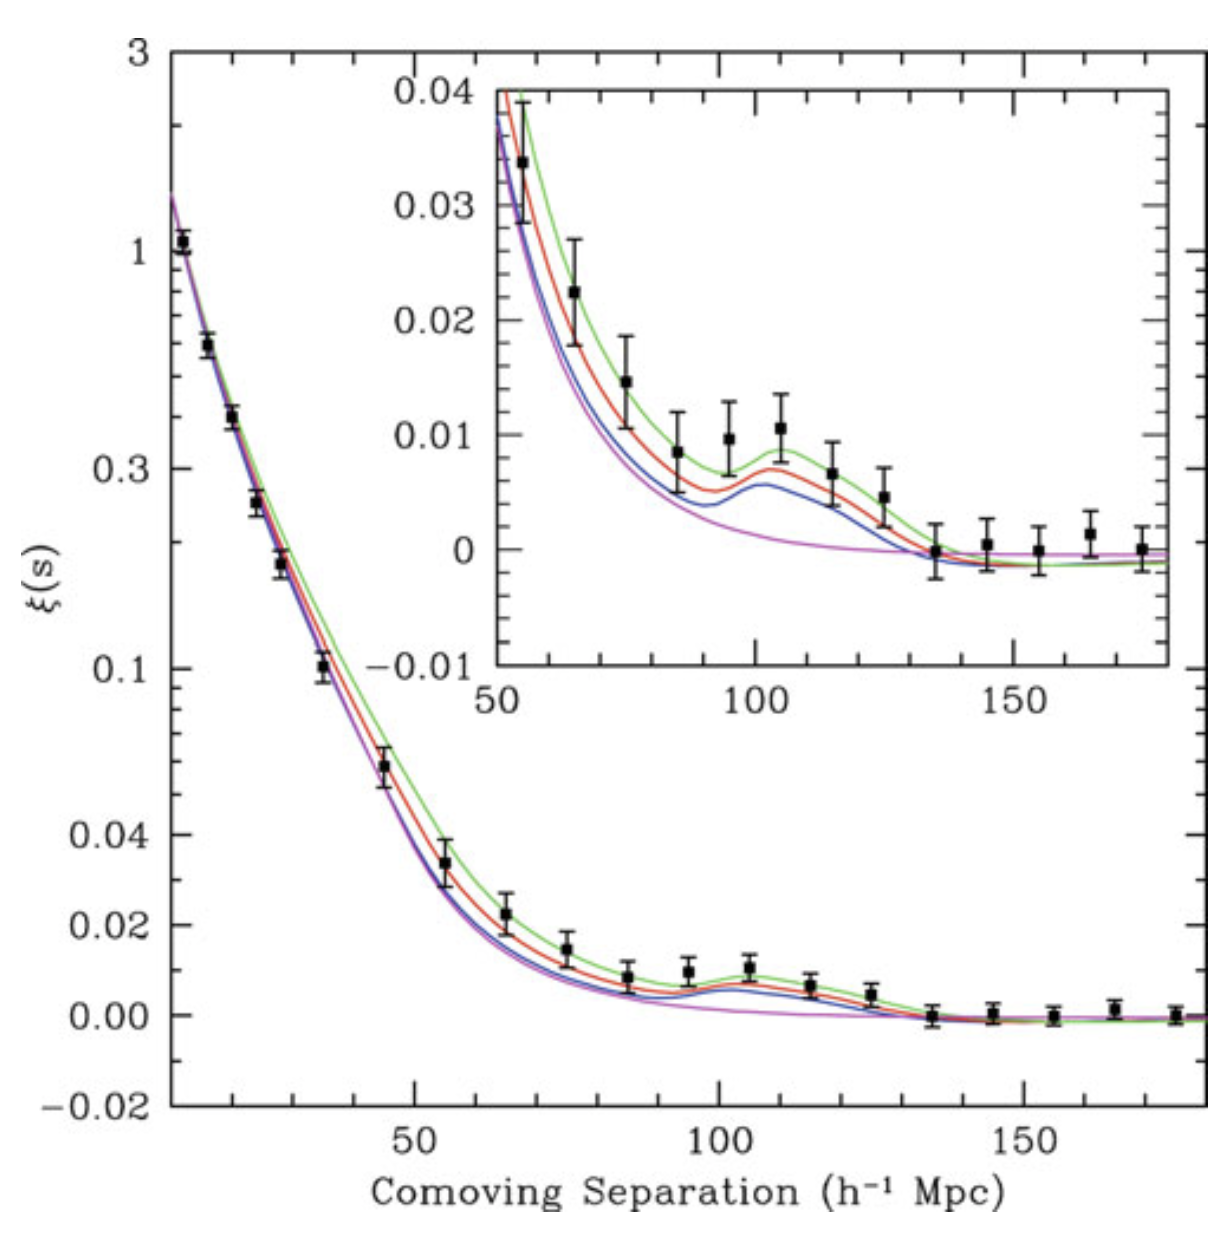
\includegraphics[width=10cm]{figures/cosmology/CorrelationFunction.png}}
\end{figure}

{\noindent}The power of the method depends on whether the galaxies trace the underlying matter distribution sufficiently well, so that the measured galaxy correlation function reflects the correlation function of matter. Given the large spatial scale on which BAOs are observed, the proportionality between the galaxy and matter fluctuation fields, assumed by the simple bias model, is expected to hold very well. This then turns BAOs into a straightforward, almost purely geometrical tool for measuring the geometry of our Universe.

{\noindent}For this reason, several surveys are underway to measure the acoustic scale as a function of redshift. Figure \ref{fig:BAOs} shows recent measurements of BAOs over a range of redshifts. Amazingly, the measurements are in perfect agreement with the cosmological parameters as determined by CMB anisotropy measurements. In particular, the spatial flatness of our Universe is confirmed, and any curvature is constrained to be very small, $\lvert\Omega_m+\Omega_\Lambda\rvert\lesssim0.01$.

\begin{figure*}[t!]
    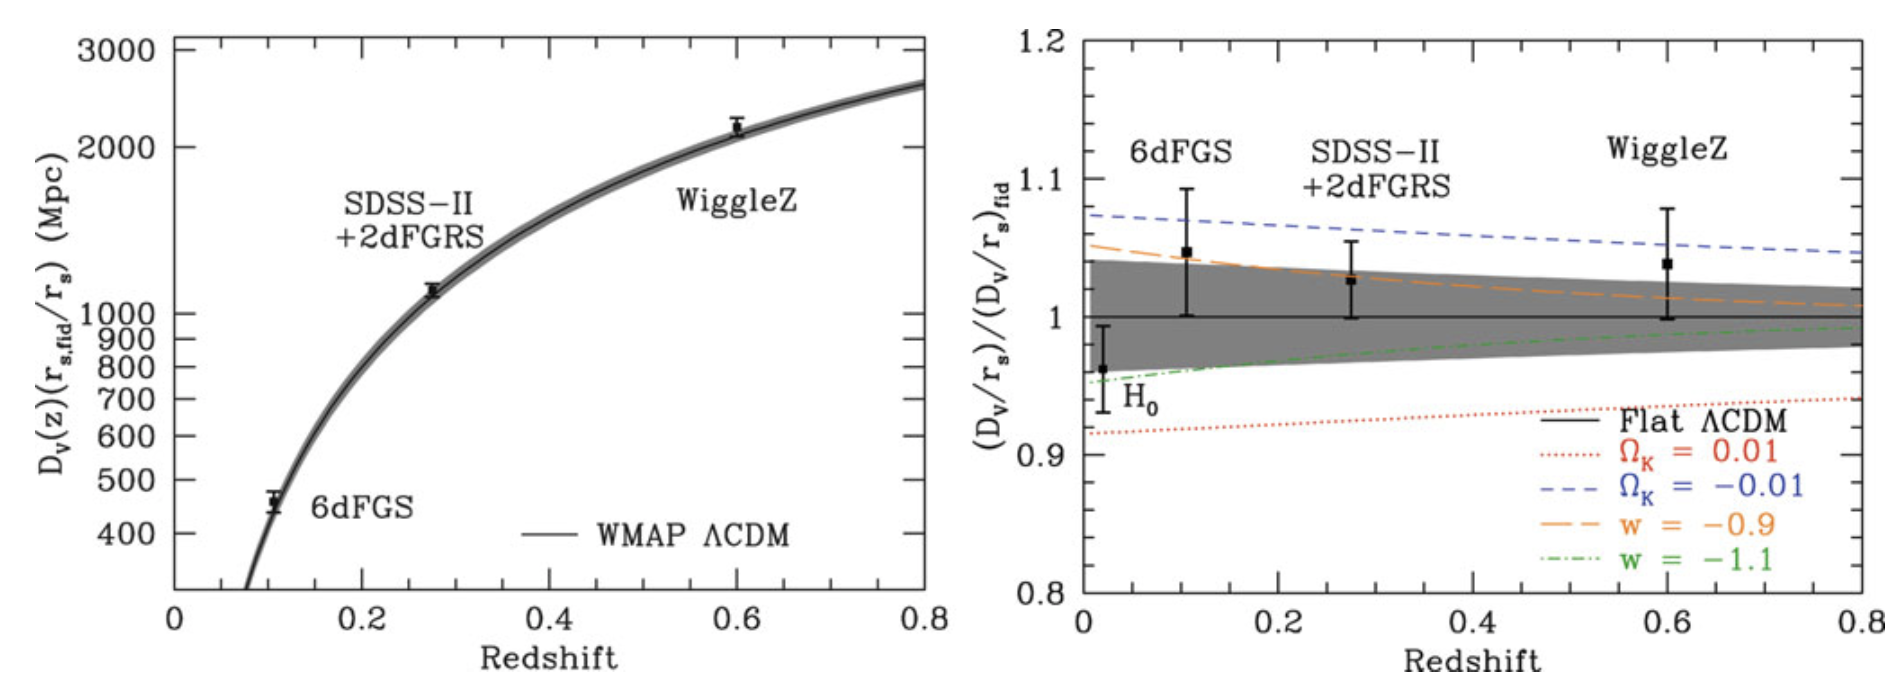
\includegraphics[width=16cm]{figures/cosmology/BAOs.png}
    \centering
    \caption{\footnotesize{Recent results on the distance-redshift relation from measurements of BAOs. Left panel: The black line and the grey band shows the best-fit cosmological model obtained from the WMAP CMB anisotropy measurements and its $1\sigma$  uncertainty range. The BAO distance determination from three surveys are indicated, which are located right on this best-fit model. Right panel: The same data are shown, now divided by the prediction of a flat $\Lambda$CDM model with parameters as determined from WMAP. Also shown are curves of this distance ratio for models with a small positive or negative curvature, or for different equations-of-state of dark energy. In particular, the BAO measurements exclude any appreciable curvature parameter of our Universe. Source: D.H. Weinberg et al. 2012, Observational Probes of Cosmic Acceleration, arXiv:1201.2434, Fig. 8. Figure taken from Schneider (2006).}}
    \label{fig:BAOs}
\end{figure*}

\newpage
\subsubsection{Follow-up Questions}

\begin{itemize}
    \item How does the CMB angular power spectrum change with cosmological parameters?
    \item How does the CMB angular power spectrum support inflation?
    \item Do we see super-horizon modes in the CMB angular power spectrum?
    \item How do we measure the CMB angular power spectrum?
    \item What about CMB polarization?
\end{itemize}


% --------------------------------------------------------------
%
%                           9. 
%
% --------------------------------------------------------------

\newpage
\subsection{Question 9}

Why is the cosmic microwave background expected to be weakly polarized, and what is practically required to observe this signal?

\subsubsection{Short answer}

The CMB is linearly polarized at the 10\% level due to \textbf{Thomson scattering} of photons off of free electrons at the surface of last scattering.  The degree of linear polarization is directly related to the quadrupole anisotropy in the photons when they last scatter. If the incoming radiation field were isotropic, orthogonal polarization states from incident directions would balance so that the outgoing radiation would remain unpolarized. Conversely, if the incident radiation field possesses a quadrupolar variation in intensity or temperature (which possess intensity peaks at $90^\circ=\pi/2$ separations), the result is a linear polarization of the scattered radiation. No other multipoles other than the quadrupole contributes to the CMB polarization.

\subsubsection{Additional context}

{\noindent}Why should we be concerned with the polarization of the cosmic microwave background (CMB) anisotropies? That the CMB anisotropies are polarized is a fundamental prediction of the gravitational instability paradigm. Under this paradigm, small fluctuations in the early Universe grow into the large scale structure we see today. If the temperature anisotropies we observe are indeed the result of primordial fluctuations, their presence at last scattering would polarize the CMB anisotropies themselves. The verification of the (partial) polarization of the CMB on small scales would thus represent a fundamental check on our basic assumptions about the behavior of fluctuations in the Universe, in much the same way that the redshift dependence of the CMB temperature is a test of our assumptions about the background cosmology. Furthermore, observations of polarization provide an important tool for reconstructing the model of the fluctuations from the observed power spectrum (as distinct from fitting an a priori model prediction from observations). \textit{The polarization probes the epoch of last scattering directly as opposed to the temperature fluctuations which may evolve between last scattering and the present}. This localization in time is a very powerful constraint for reconstructing the sources of anisotropy. Moreover, different sources of temperature anisotropies (scalar, vector, and tensor) give different patterns in the polarization: both in its intrinsic structure and in its correlation with the temperature fluctuations themselves. Thus by including polarization information, one can distinguish the ingredients which go to make up the temperature power spectrum and so the cosmological model. Finally, the polarization power spectrum provides information complementary to the temperature power spectrum even for ordinary (scalar or density) perturbations. This can be of use in breaking parameter degeneracies and thus constraining cosmological parameters more accurately. The prime example of this is the degeneracy, within the limitations of cosmic variance, between a change in the normalization and an epoch of ``late'' reionization.

{\noindent}Yet how polarized are the fluctuations? The degree of linear polarization is directly related to the quadrupole anisotropy in the photons when they last scatter. While the exact properties of the polarization depend on the mechanism for producing the anisotropy, several general properties arise. The polarization peaks at angular scales smaller than the horizon at last scattering due to causality. Furthermore, the polarized fraction of the temperature anisotropy is small since only those photons that last scattered in an optically thin region could have possessed a quadrupole anisotropy. The fraction depends on the duration of last scattering. For the standard thermal history, it is 10\% on a characteristic scale of tens of arcminutes. Since temperature anisotropies are at the $10^{-5}$ level, the polarized signal is at (or below) the $10^{-6}$ level, or several $\mu\mathrm{K}$ representing a significant experimental challenge.

{\noindent}The Thomson scattering cross section $\sigma_T$ depends on polarization as (see, e.g., Chandrasekhar, 1960) as 

\begin{align*}
    \frac{\mathrm{d}\sigma_T}{\mathrm{d}\Omega} \propto \lvert \bm{\epsilon}\cdot\bm{\epsilon}' \rvert^2,
\end{align*}

{\noindent}where $\bm{\epsilon}$ and $\bm{\epsilon}'$ are the incident and scattered polarization directions, and $\Omega$ is the solid angle. Heuristically, the incident light sets up oscillations of the target electron in the direction of the electric field vector $E$ (i.e., the polarization). The scattered radiation intensity thus peaks in the direction normal to, with polarization parallel to, the incident polarization. More formally, the polarization dependence of the cross section is dictated by electromagnetic gauge invariance and thus follows from very basic principles of fundamental physics.

\begin{figure}[h]
    \floatbox[{\capbeside\thisfloatsetup{capbesideposition={right,top},capbesidewidth=4cm}}]{figure}[\FBwidth]
    {\caption{\footnotesize{\\Thomson scattering of radiation with a quadrupole anisotropy generates linear polarization. Blue colors (thick lines) represent hot and red colors (thin lines) cold radiation. Figure taken from Hu \& White (1997).}}
    \label{fig:Thomsonscattering}}
    {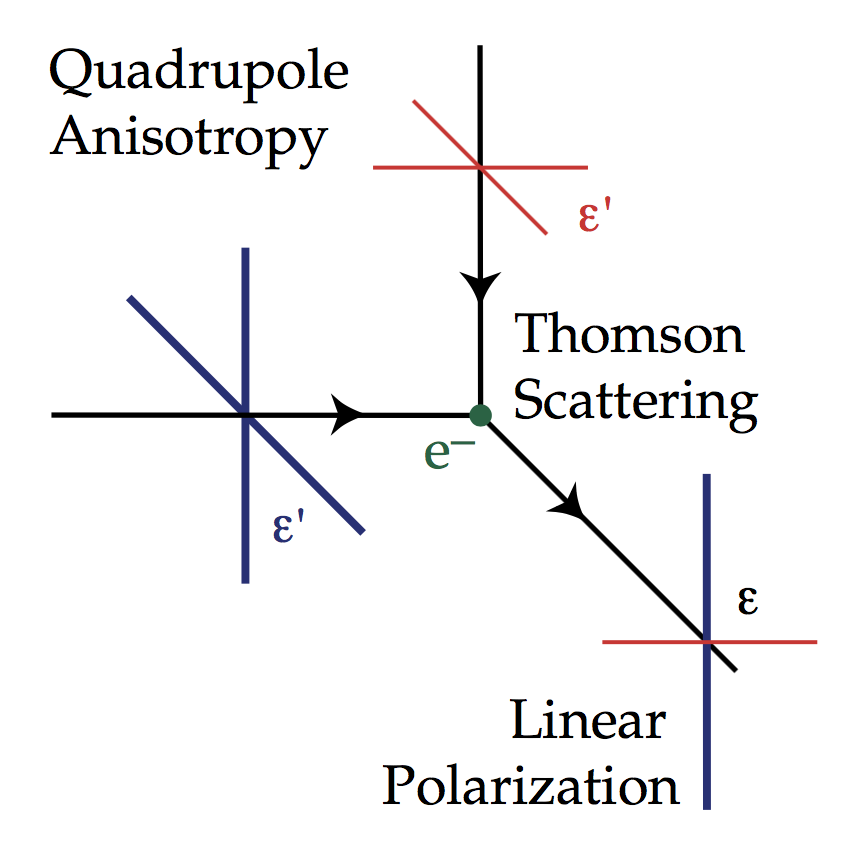
\includegraphics[width=8cm]{figures/cosmology/ThomsonScattering.png}}
\end{figure}

{\noindent}If the incoming radiation field were isotropic, orthogonal polarization states from incident directions separated by $90^\circ$ would balance so that the outgoing radiation would remain unpolarized. Conversely, if the incident radiation field possesses a quadrupolar variation in intensity or temperature (which possess intensity peaks at $90^\circ=\pi/2$ separations), the result is a linear polarization of the scattered radiation (see Figure \ref{fig:Thomsonscattering}). A reversal in sign of the temperature fluctuation corresponds to a $90^\circ$ rotation of the polarization, which reflects the spin-$2$ nature of polarization.

{\noindent}In terms of a multipole decomposition of the radiation field into spherical harmonics, $Y_\ell^m(\theta,\phi)$, the five quadrupole moments are represented by $\ell= 2, m=0,\pm1,\pm2$. The orthogonality of the spherical harmonics guarantees that no other moment can generate polarization from Thomson scattering. In these spherical coordinates, with the north pole at $\theta=0$, we call a N-S (E-W) polarization component $Q>0$ ($Q<0$) and a NE-SW (NW-SE) component $U>0$ ($U<0$). The polarization amplitude and angle clockwise from north are

\begin{align*}
    P = \sqrt{Q^2+U^2}
\end{align*}

{\noindent}and

\begin{align*}
    \chi = \frac{1}{2}\arctan\left(\frac{U}{Q}\right).
\end{align*}

{\noindent}where $P$ is the polarized intensity and $Q$ and $U$ are the linear polarization Stokes vectors.

{\noindent}If Thomson scattering is rapid, then the randomization of photon directions that results destroys any quadrupole anisotropy and polarization. The problem of understanding the polarization pattern of the CMB thus reduces to understanding the quadrupolar temperature fluctuations at last scattering. Temperature perturbations have 3 geometrically distinct sources: the scalar (compressional), vector (vertical) and tensor (gravitational wave) perturbations. Formally, they form the irreducible basis of the symmetric metric tensor. We shall consider each of these in Question 17 and show that the scalar, vector, and tensor quadrupole anisotropy correspond to $m=0,\pm1,\pm2$ respectively. This leads to different patterns of polarization for the three sources.

\subsubsection{Follow-up Questions}

\begin{itemize}
    \item What are some foregrounds or challenges to observing this signal?
    \item Why does dust polarize the CMB?
    \item Why is dust not randomly oriented?
    \item How did we first determine that dust is not randomly oriented?
\end{itemize}

% --------------------------------------------------------------
%
%                           10. 
%
% --------------------------------------------------------------

\newpage
\subsection{Question 10}

Our view of the cosmic microwave background is affected by what is along the line of sight. Give two examples of CMB foregrounds that also provide information about the cosmic parameters.

\subsubsection{Short answer}

\begin{itemize}
    \item \textbf{Thermal Sunyaev-Zeldovich effect}: Electrons in the hot gas of the intracluster medium can inverse Compton scatter photons of the CMB. Since galaxy clusters are separated by $\sim150\,{\rm Mpc}$, this will increase the power of the first peak in the CMB power spectrum and can inform us about $\Omega_m$.
    \item \textbf{Integrated Sachs-Wolfe effect}: Inhomogeneities  in  the  gravitational  potential  cause photons which originate in regions of higher density to climb out of a potential well. As a result of this, they lose energy and are gravitationally redshifted. This is a primary anisotropy effect which dominates on superhorizon scales.
\end{itemize}

\subsubsection{Additional context}

{\noindent}The CMB consists of photons that last interacted with matter at $z\sim1100$. Since the Universe must already have been inhomogeneous at this time, in order for the structures present in the current Universe to be able to form, it is expected that these spatial inhomogeneities are visible as a (small) anisotropy of the CMB: the angular distribution of the CMB temperature reflects the matter inhomogeneities at the redshift of decoupling of radiation and matter.

{\noindent}Since the discovery of the CMB in 1965, such anisotropies have been searched for. Under the assumption that the matter in the Universe solely consists of baryons, the expectation was that we would find relative fluctuations in the CMB temperature of amplitude $\Delta T/T10^{-3}$ on scales of a few arcminutes. This expectation is based on the theory of gravitational instability for structure growth: to account for the density fluctuations observed today where the density contrast $\delta\sim1$ on scales of $\sim10h^{-1}\,{\rm Mpc}$, one needs relative density fluctuations at $z\sim1000$ of order $D_+(z=1000)\sim10^{-3}$. Despite increasingly more sensitive observations, such fluctuations were not detected. The upper limits resulting from these searches for anisotropies provided one of the arguments that, in the mid-1980s, caused the idea of the existence of dark matter on cosmic scales to increasingly enter the minds of cosmologists. In a Universe which is dominated by dark matter the expected CMB fluctuations on small angular scales are considerably smaller than in a purely baryonic Universe. It was the COBE satellite with which temperature fluctuations in the CMB were finally observed in 1992 (Figure \ref{fig:cmbcobe}), a discovery which was awarded the Physics Nobel Prize in 2006. Over the following years, sensitive and significant measurements of the CMB anisotropy were carried out using balloons and ground-based telescopes. Two more satellites have observed the full microwave sky, WMAP and Planck; their results, together with ground-based measurements at smaller angular scales, have yielded the most stringent constraints on cosmological parameters yet.

\begin{figure}[t]
    \floatbox[{\capbeside\thisfloatsetup{capbesideposition={right,top},capbesidewidth=4cm}}]{figure}[\FBwidth]
    {\caption{\footnotesize{Temperature distribution of the CMB on the sky as measured by the COBE satellite. The top image shows a dipole distribution; it originates from the Earth's motion relative to the restframe of the CMB. Our Solar System moves at a speed of $369\,{\rm km\,s^{-1}}$ relative to that system, which leads to a dipole anisotropy with an amplitude of $\Delta T/T\sim v/c\sim1.2\times10^{-3}$ due to the Doppler effect. If this dipole contribution is subtracted, we get the map in the middle which clearly shows the emission from the Galactic disk. Since this emission has a different spectral energy distribution (it is not a blackbody of $T\sim3\,{\rm K}$), it can also be subtracted to get the temperature map at the bottom. These are the primordial fluctuations of the CMB, with an amplitude of about  $\Delta T/T\sim2\times10^{-5}$. Credit: COBE/DRM team, NASA. Figure taken from Schneider (2006).}}
    \label{fig:cmbcobe}}
    {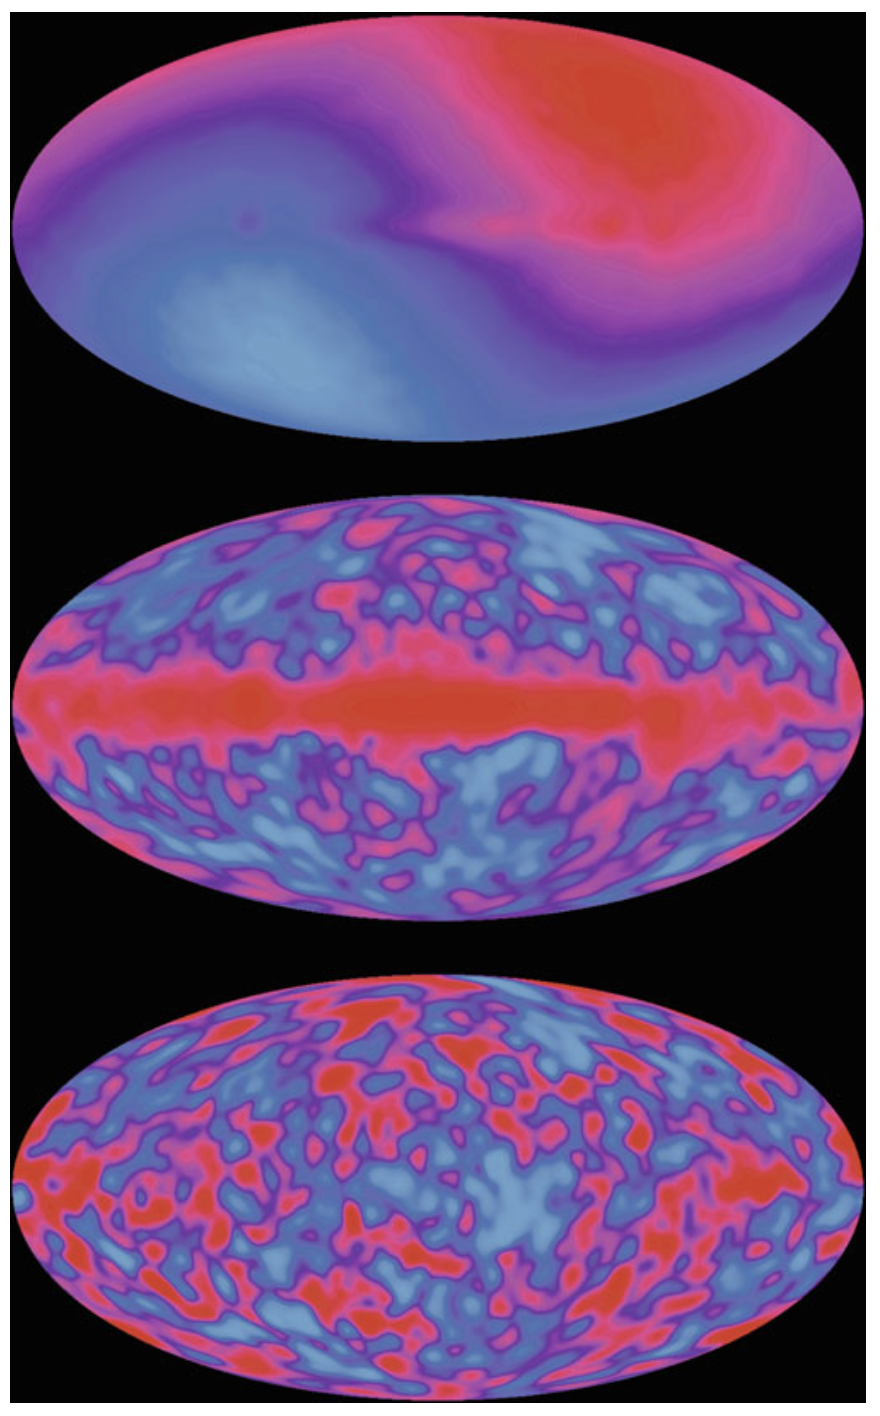
\includegraphics[width=10cm]{figures/cosmology/CMBCOBE.png}}
\end{figure}

{\noindent}The CMB anisotropies depend on nearly all cosmological parameters, such as $\Omega_m$, $\Omega_b$, $\Omega_\Lambda$, $\Omega_\mathrm{HDM}$, $H_0$, the normalization $\sigma_8$, the primordial slope $n_s$, and the shape parameter $\Gamma$ of the power spectrum. Therefore, from an accurate mapping of the angular distribution of the CMB and by comparison with theoretical expectations, all these parameters can, in principle, be determined.

{\noindent}Temperature fluctuations originating at the time of last scattering are called primary anisotropies. Later, as the CMB photons propagate through the Universe, they may experience a number of distortions along their way which, again, may change their temperature distribution on the sky. These effects then lead to secondary anisotropies.

{\noindent}Given that the amplitude of the polarization is so small the question of foregrounds is even more important than for the temperature anisotropy. Unfortunately, the level and structure of the various foreground polarization in the CMB frequency bands is currently not well known. Atmospheric emission is believed to be negligibly polarized, leaving the main astrophysical foregrounds: free-free, synchrotron, dust, and point source emissions. Of these the most important foreground is synchrotron emission.

{\noindent}Free-free emission (bremsstrahlung) is intrinsically unpolarized but can be partially polarized by Thomson scattering within the HII region. This small effect is not expected to polarize the emission by more than 10\%. The emission is larger at low frequencies but is not expected to dominate the polarization at any frequency.

{\noindent}The polarization of dust is not well known. In principle, emission from dust particles could be highly polarized, however it's been found that that the majority of dust is polarized at the $\approx2\%$ level at $100\mu{\rm m}$ with a small fraction of regions approaching 10\% polarization. It's also been shown that even at 100\% polarization, extrapolation of the IRAS $100\mu{\rm m}$ map with the COBE FIRAS index shows that dust emission is negligible below $80\,{\rm GHz}$. At higher frequencies it will become the dominant foreground.

{\noindent}Radio point sources are polarized due to synchrotron emission at $<20\%$ level. For large angle experiments, the random contribution from point sources will contribute negligibly, but may be of more concern for the upcoming satellite missions.

{\noindent}Galactic synchrotron emission is the major concern. It is potentially highly polarized with the fraction dependent on the spectral index and depolarization from Faraday rotation and non-uniform magnetic fields. The level of polarization is expected to lie between 10\%-75\% of a total intensity which itself is approximately $5\,\mu{\rm K}$ at $30\,{\rm GHz}$. This estimate follows from extrapolating measurements at $1411\,{\rm MHz}$ with an index of $T\propto\nu^{-3}$.

{\noindent}Due to their different spectral indices, the minimum in the foreground polarization, like the temperature, lies near $100\,{\rm GHz}$. For full sky measurements, since synchrotron emission is more highly polarized than dust, the optimum frequency at which to measure intrinsic (CMB) polarization is slightly higher than for the anisotropy. Over small regions of the sky where one or the other of the foregrounds is known a priori to be absent the optimum frequency would clearly be different. However as with anisotropy measurements, with multi-frequency coverage, polarized foregrounds can be removed.

{\noindent}It is also interesting to consider whether the spatial as well as frequency signature of the polarization can be used to separate foregrounds. Using angular power spectra for the spatial properties of the foregrounds is a simple generalization of methods already used in anisotropy work. For instance, in the case of synchrotron emission, if the spatial correlation in the polarization follows that of the temperature itself, the relative contamination will decrease on smaller angular scales due to its diffuse nature. Furthermore the peak of the cosmic signal in polarization occurs at even smaller angular scales than for the anisotropy.

{\noindent}Of those that can provide information about the cosmic parameters...

{\noindent}\textbf{The thermal Sunyaev-Zeldovich effect}: Electrons in the hot gas of the intracluster medium (ICM) can inverse Compton scatter photons of the CMB. The optical depth and thus the scattering probability for this inverse Compton scattering is relatively low, but the effect is nevertheless observable and, in addition, is of great importance for the analysis of clusters. A photon moving through a cluster of galaxies towards us will change its direction through scattering and thus will not reach us. But since the cosmic background radiation is isotropic, for any CMB photon that is scattered out of the line-of-sight, another photon exists -- statistically -- that is scattered into it, so that the total number of photons reaching us is preserved. However, the energy of the photons changes slightly through scattering by the hot electrons, in a way that they have an (on average) higher frequency after scattering. Hence, by this inverse Compton scattering, energy is on average transferred from the electrons to the photons, as can be seen in Figure \ref{fig:szeffect}.

\begin{figure}[h]
    \floatbox[{\capbeside\thisfloatsetup{capbesideposition={right,top},capbesidewidth=4cm}}]{figure}[\FBwidth]
    {\caption{\footnotesize{The influence of the Sunyaev-Zeldovich effect on the cosmic background radiation. The dashed curve represents the Planck distribution of the unperturbed CMB spectrum, the solid curve shows the spectrum after the radiation has passed through a cloud of hot electrons. The magnitude of this effect, for clarity, has been very much exaggerated in this sketch. Source: Carlstrom et al. 2002, ARA\&A 40, 643. Image taken from Schneider (2006).}}
    \label{fig:szeffect}}
    {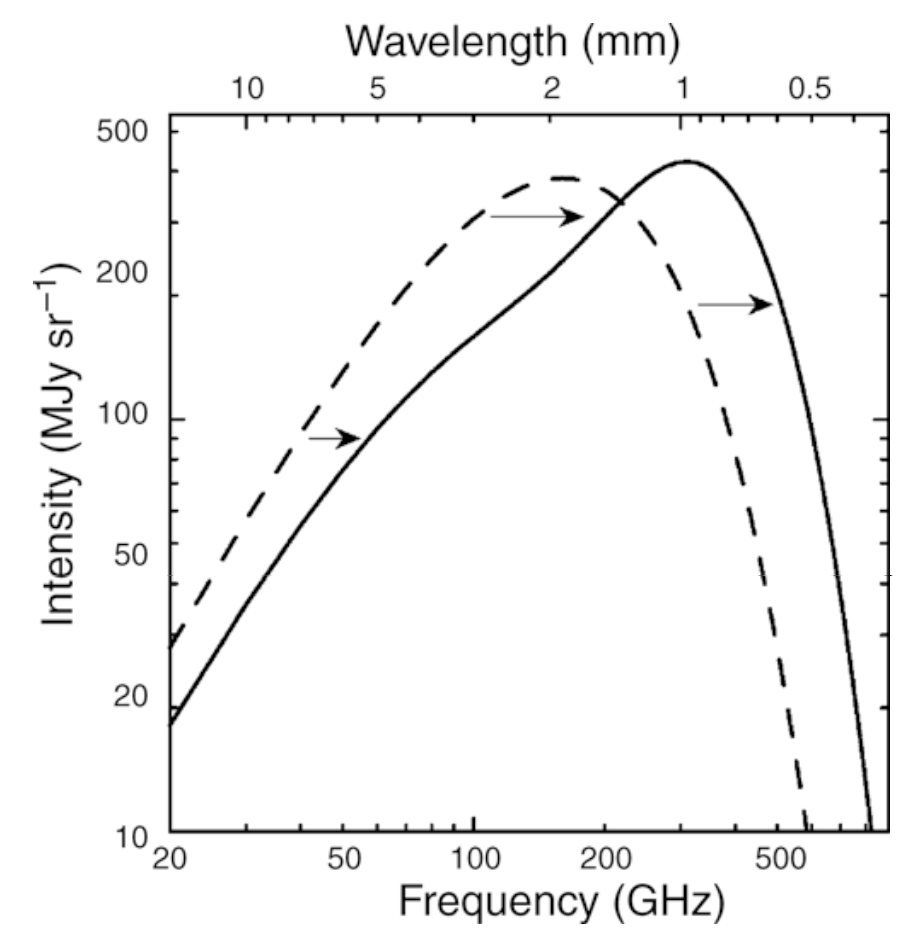
\includegraphics[width=8cm]{figures/cosmology/SZeffect.png}}
\end{figure}

{\noindent}In the Rayleigh-Jeans (RJ) domain of the CMB spectrum, at wavelengths larger than about $2\,{\rm mm}$, the intensity of the CMB is decreased by the SZ-effect. For the change in specific intensity in the RJ part, one obtains

\begin{align*}
    \frac{\Delta I_\nu^\mathrm{RJ}}{I_\nu^\mathrm{RJ}} = -2y,
\end{align*}

{\noindent}where $y$ is the the Compton y-parameter

\begin{align*}
    y = \int\frac{k_BT}{m_ec^2}\sigma_Tn_e\mathrm{d}l
\end{align*}

{\noindent}and $\sigma_T$ is the Compton cross-section for electron scattering

\begin{align*}
    \sigma_T = \frac{8\pi}{3}\left(\frac{e^2}{m_ec^2}\right)^2 = \frac{8\pi}{3}e_{e,0}^2 ~ [{\rm m^2}].
\end{align*}

{\noindent}Obviously, $y$ is proportional to the optical depth with respect to Compton scattering, given as an integral over $n_e\sigma_T$ along the line-of-sight. Furthermore, $y$ is proportional to the gas temperature, because that defines the average energy transfer per scattering event. Overall, $y$ is proportional to the integral over the gas pressure $P D=nk_BT$ along the line-of-sight through the cluster.

{\noindent}The SZ effect affects the temperature distribution of the CMB. Some of the photons propagating along lines-of-sight passing through clusters of galaxies or other regions of dense and hot gas are scattered by the hot electrons, resulting in a temperature change in these directions. We recall that in the direction of clusters the measured intensity of the CMB radiation is reduced at low frequencies, whereas it is increased at high frequencies. Hence, the SZ effect can be identified in the CMB data if measurements are conducted over a sufficiently large frequency range.

{\noindent}The SZE spectral distortion of the CMB expressed as a temperature change $\Delta T_\mathrm{SZE}$ at dimensionless frequency $x\equiv h\nu k_BT_\mathrm{CMB}$ is given by

\begin{align*}
    \frac{\Delta T_\mathrm{SZE}}{T_\mathrm{CMB}} = f(x)y = f(x)\int n_e\frac{k_BT_e}{m_ec^2}\sigma_T \mathrm{d}l ~ [{\rm dimensionless}],
\end{align*}

{\noindent}where $y$ is the Compton y-parameter, which for an isothermal cluster equals the optical depth, $\tau_e$, times the fractional energy gain per scattering, $\sigma_T$ is the Thomson cross-section, $n_e$ is the electron number density, $T_e$ is the electron temperature, $k_B$ is the Boltzmann constant, $m_ec^2$ is the electron rest mass energy, and the integration is along the line of sight. The frequency dependence of the SZE is 

\begin{align*}
    f(x) = x\left(\frac{e^x+1}{e^x-1}\right)(1+\delta_\mathrm{SZE}()bx,T_e) ~ [{\rm dimensionless}],
\end{align*}

{\noindent}where $\delta_\mathrm{SZE}(x,T_e)$ is the relativistic correction to the frequency dependence. Note that $f(x)\rightarrow-2$ in the nonrelativistic and Rayleigh-Jeans (RJ) limits.

{\noindent}It is worth noting that $\Delta T_\mathrm{SZE}/T_\mathrm{CMB}$ is independent of redshift. This unique feature of the SZE makes it a potentially powerful tool for investigating the high-redshift Universe.

\begin{figure}[t]
    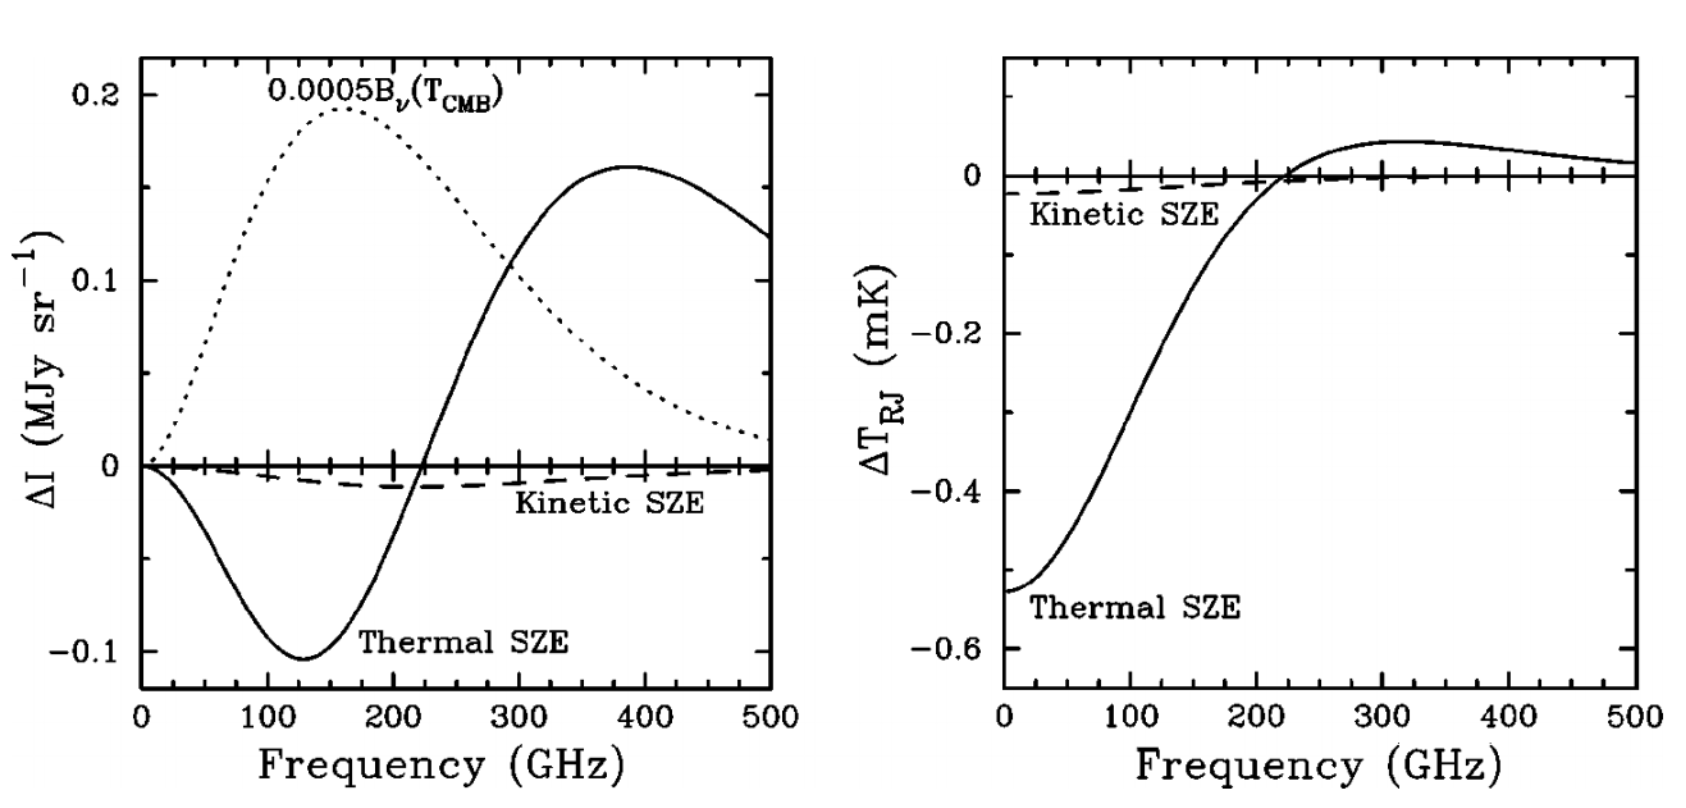
\includegraphics[width=16cm]{figures/cosmology/SZrealistic.png}
    \centering
    \caption{\footnotesize{Spectral distortion of the CMB radiation due to the SZE. The left panel shows the intensity and the right panel shows the RJ brightness temperature. The thick solid line is the thermal SZE and the dashed line is the kinetic SZE. For reference the $2.7\,{\rm K}$ thermal spectrum for the CMB intensity scaled by $0.0005$ is shown by the dotted line in the left panel. The cluster properties used to calculate the spectra are an electron temperature of $10\,{\rm keV}$, a Compton $y$ parameter of $10^{-4}$, and a peculiar velocity of $500\,{\rm km\,s^{-1}}$. Image taken from Carlstrom (2002).}}
    \label{fig:szrealistic}
\end{figure}

{\noindent}The spectral distortion of the CMB spectrum by the thermal SZE is shown in Figure \ref{fig:szrealistic} (solid line) for a realistic massive cluster ($y=10^{-4}$) in units of intensity (left panel) and RJ brightness temperature (right panel). The RJ brightness is shown because the sensitivity of a radio telescope is calibrated in these units. It is defined simply by $I_\nu=(2k_B\nu^2/c^2)T_\mathrm{RJ}$, where $I_\nu$ is the intensity at frequency $\nu$, $k_B$ is Boltzmann's constant, and $c$ is the speed of light. The CMB blackbody spectrum, $B_\nu(T_\mathrm{CMB})$, multiplied by $0.0005$ (dotted line) is also shown for comparison. Note that the spectral signature of the thermal effect is distinguished readily from a simple temperature fluctuation of the CMB. The kinetic SZE distortion is shown by the dashed curve. In the nonrelativistic regime it is indistinguishable from a CMB temperature fluctuation.

{\noindent}The most important features of the thermal SZE are that (a) it is a small spectral distortion of the CMB of order $\sim1\,{\rm mK}$, which is proportional to the cluster pressure integrated along the line of sight; (b) it is independent of redshift; (c) it has a unique spectral signature with a decrease in the CMB intensity at frequencies $\lesssim218\,{\rm GHz}$ and an increase at higher frequencies; and (d) the integrated SZE flux is proportional to the temperature-weighted mass (total thermal energy) of the cluster, implying that SZE surveys will have a mass threshold nearly independent of redshift.

{\noindent}\textbf{The kinetic Sunyaev-Zeldovich effect}: If the cluster is moving with respect to the CMB rest frame, there will be an additional spectral distortion due to the Doppler effect of the cluster bulk velocity on the scattered CMB photons. If a component of the cluster velocity, $v_\mathrm{pec}$, is projected along the line of sight to the cluster, then the Doppler effect will lead to an observed distortion of the CMB spectrum referred to as the kinetic SZE. In the nonrelativistic limit the spectral signature of the kinetic SZE is a pure thermal distortion of magnitude

\begin{align*}
    \frac{\Delta T_\mathrm{SZ}}{T_\mathrm{CMB}} = -\tau_e \left(\frac{v_\mathrm{pec}}{c}\right) ~ [{\rm dimensionless}],
\end{align*}

{\noindent}where $v_\mathrm{pec}$ is along the line of sight; i.e., the emergent spectrum is still described completely by a Planck spectrum, but at a slightly different temperature, lower (higher) for positive (negative) peculiar velocities (see Figure \ref{fig:szrealistic}).

{\noindent}The scattering of the CMB photons by the hot intracluster medium (ICM) electrons can result in polarization at levels proportional to powers of ($v_\mathrm{pec}/c$) and $\tau_e$. The largest polarization is expected from the anisotropic optical depth to a given location in the cluster. For example, toward the outskirts of a cluster one expects to see a concentric (radial) pattern of the linear polarization at frequencies at which the thermal SZE is positive (negative). Nonspherical morphology for the electron distributions will lead to considerably complicated polarization patterns. The peak polarization of this signal will be of order $\tau_e$ times the SZE signal (i.e., of order $0.025(k_BT_e/m_ec^2)\tau_e^2$ times the CMB intensity). For a massive cluster with $\tau_e=0.01$, the effect would be at the $0.1\,{\mu K}$ level toward the edge of the cluster. In principle, this effect could be used to measure the optical depth of the cluster and therefore separate $T_e$ and $\tau_e$ from a measurement of the thermal SZE.

{\noindent}It can be shown that polarization of the SZE comes entirely from the quadrupole component of the local radiation field experienced by the scattering electron. In the case above, the quadrupole component at the outskirts of the cluster is caused by the anisotropy in the radiation field in the direction of the cluster center due to the SZE. Sunyaev and Zel'dovich discussed polarization due to the motion of the cluster with respect to the CMB and transverse to our line of sight. In this case, the quadrupole comes from the Doppler shift. They found the largest terms to be of order $0.1\tau_e(v_\mathrm{pec}/c)^2$ and $0.025\tau_e^2(v_\mathrm{pec}/c$) of the CMB intensity. The latter term, second order in $\tau_e$, can be thought of as imperfect cancellation of the dipole term due to the anisotropic optical depth. Using $\tau_e=0.01$ and a bulk motion of $500\,{\rm km\,s-1}$ results in polarization levels of order $10\,{\mu K}$, far beyond the sensitivity of current instrumentation.

{\noindent}The CMB as seen by the cluster electrons will have a quadrupole component and therefore the electron scattering will lead to linear polarization. This mechanism could possibly be used to trace the evolution of the CMB quadrupole if polarization measurements could be obtained for a large number of clusters binned in direction and redshift. Sazonov and Sunyaev calculated the expected polarization level and found that the maximum CMB quadrupole-induced polarization is $50(\tau_e/0.01)\,{\rm \mu K}$, somewhat higher than the expected velocity-induced terms discussed above. The effect is again too small to expect detection in the near future. However, by averaging over many clusters, detecting this polarization might be possible with future satellite missions.

{\noindent}\textbf{The integrated Sachs-Wolfe effect}: Inhomogeneities in the gravitational potential cause photons which originate in regions of higher density to climb out of a potential well. As a result of this, they lose energy and are redshifted (gravitational redshift). This effect is partly compensated for by the fact that, besides the gravitational redshift, a gravitational time delay also occurs: a photon that originates in an overdense region will be scattered at a slightly earlier time, and thus at a slightly higher temperature of the Universe, compared to a photon from a region of average density. Both effects always occur side by side. They are combined under the term Sachs-Wolfe effect. Its separation into two processes is necessary only in a simplified description; a general relativistic treatment of the Sachs-Wolfe effect jointly yields both processes.

\subsubsection{Follow-up Questions}

\begin{itemize}
    \item How does the thermal Sunyaev-Zeldovich effect compare to the kinetic Sunyaev-Zeldovich effect?
    \item How do we actually measure the SZ effect?
    \item What is the redshift dependence of the SZ effect? (There is none!)
    \item How do we actually measure the integrated Sachs-Wolfe effect?
\end{itemize}


% --------------------------------------------------------------
%
%                           11. 
%
% --------------------------------------------------------------

\newpage
\subsection{Question 11}

Describe cosmological inflation. List at least three important observations it is intended to explain.

\subsubsection{Short answer}

Inflation can most generally be defined as a period of exponential expansion of the form

\begin{align*}
    a(t) \propto e^{Ht} ~ [{\rm dimensionless}]
\end{align*}

{\noindent}in the very early Universe ($t\sim10^{-35}\,{\rm s}$). Inflation is intended to explain:

\begin{itemize}
    \item \textbf{The flatness problem}. This can be states as ``The Universe is nearly flat today, and was even flatter in the past.'' 
    \item \textbf{The horizon problem}. This can be states as ``The Universe is nearly isotropic and homogeneous today, and was even more so in the past.''
    \item \textbf{The magnetic monopole problem}. This can be states as ``The Universe is apparently free of magnetic monopoles.''
\end{itemize}

{\noindent}Inflation explains these puzzling aspects of our Universe, by flattening it, ensuring its homogeneity over large scales, and driving down the number density of magnetic monopoles which it contains. At present, there is not a consensus among cosmologists about the exact mechanism driving inflation.

\subsubsection{Additional context}

In the early 1980s, a model was developed which was able to solve the flatness and horizon problems (and some others as well). As a motivation for this model, we first recall that the physical laws and properties of elementary particles are well known up to energies of $\sim100\,{\rm GeV}$ because they were experimentally tested in particle accelerators. For higher energies, particles and their interactions are unknown. This means that the history of the Universe can be considered secure only up to energies of $\sim100\,{\rm GeV}$. The extrapolation to earlier times, up to the Big Bang, is considerably less certain. From particle physics we expect new phenomena to occur at an energy scale of the Grand Unified Theories (GUTs), at about $10^{14}\,{\rm GeV}$, corresponding to $t\sim10^{-34}\,{\rm s}$.

{\noindent}In the inflationary scenario it is presumed that at very early times the vacuum energy density was much higher than today, so that it dominated the Hubble expansion. Then $\dot{a}/a\approx\sqrt{\Lambda/3}$. This implies an exponential expansion of the Universe,

\begin{align*}
    a(t) = Ce^{\sqrt{\frac{\Lambda}{3}}t} ~ [{\rm dimensionless}]
\end{align*}

{\noindent}Obviously, this exponential expansion (or inflationary phase) cannot last forever. We assume that a phase transition took place in which the vacuum energy density is transformed into normal matter and radiation (a process called reheating), which ends the exponential expansion and after which the normal Friedmann evolution of the Universe begins. Figure \ref{fig:inflation} sketches the expansion history of the universe in an inflationary model.

\begin{figure}[h]
    \floatbox[{\capbeside\thisfloatsetup{capbesideposition={right,top},capbesidewidth=4cm}}]{figure}[\FBwidth]
    {\caption{\footnotesize{During an inflationary phase, indicated here by the gray bar, the Universe expands exponentially. This phase comes to an end when a phase transition transforms the vacuum energy into matter and radiation, after which the Universe follows the normal Friedmann expansion. Adapted from: Alan Guth 1998, The inflationary Universe, Basic Books. Figure taken from Schneider (2006).}}
    \label{fig:inflation}}
    {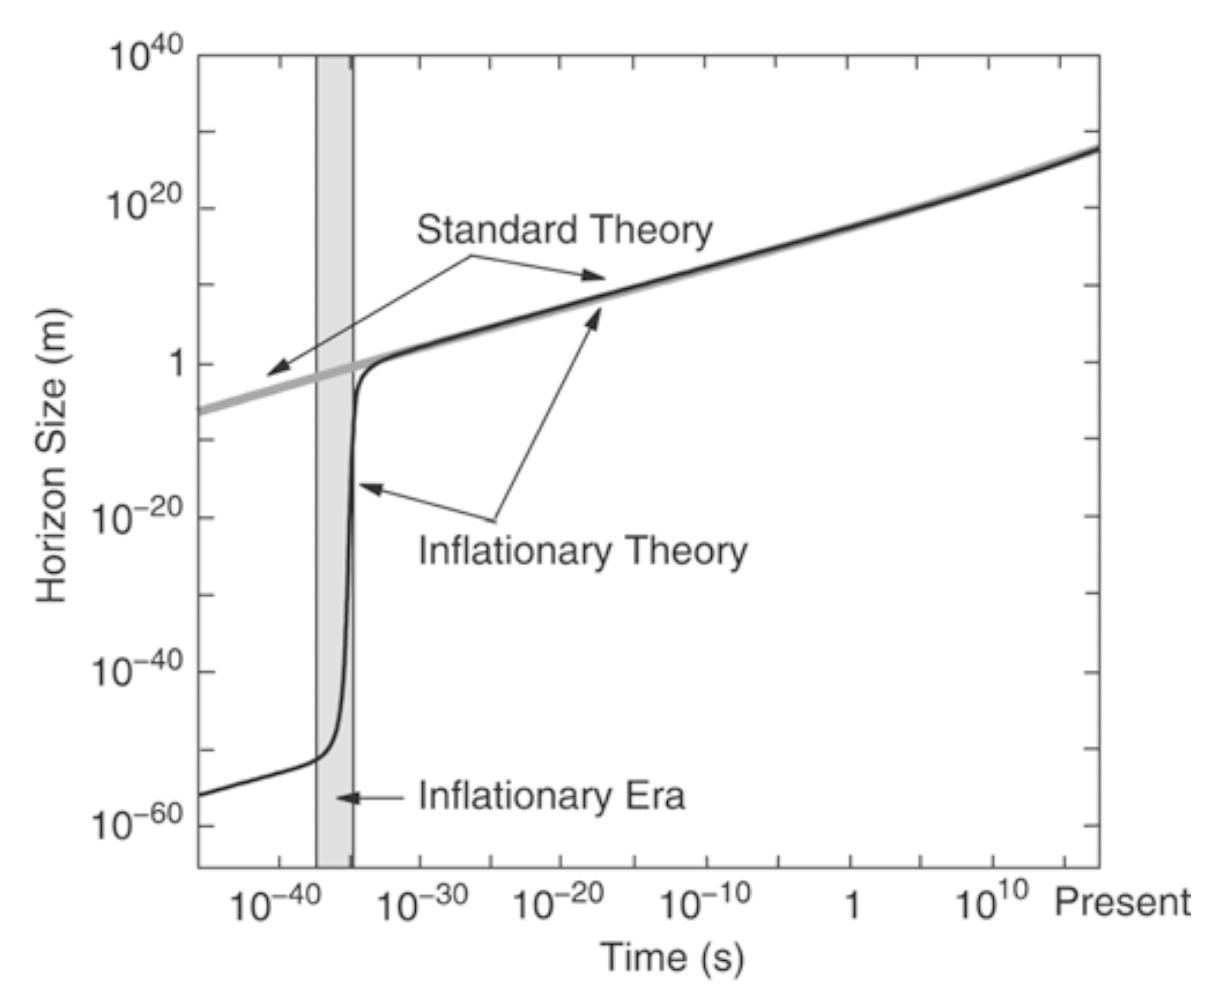
\includegraphics[width=9cm]{figures/cosmology/Inflation.png}}
\end{figure}

{\noindent}At present, there is not a consensus among cosmologists about the exact mechanism driving inflation; there is no known scalar field which can drive inflation. (A skeptic might point out that there is no known fundamental scalar held at all!) Therefore, it may well be true that the idea of inflation is correct but it is driven by something other than a scalar field. Having said that, there are a number of reasons to work with scalar fields, as we will do whenever we need to specify the source of inflation. Almost all fundamental particle physics theories contain scalar fields. In fact, historically it was particle physicists studying high-energy extensions of the Standard Model (in particular GUTs) who proposed the idea of inflation driven by a scalar field as a natural byproduct of some of these extensions. Indeed, almost all current work on inflation is based on a scalar field (or sometimes two). The alternative from a particle physics point of view is to use a vector field (such as the electromagnetic potential) or a set of fermions (similar to the way condensates induce superconductivity) to drive inflation. Neither of these choices works very well, but they both complicate things severely, so we will stick to a scalar field.

{\noindent}\textbf{The horizon problem}: The finite speed of light implies that we are only able to observe a finite part of the Universe, namely those regions from which light can reach us within a time $t_0$. Since $t0\approx13.8\,{\rm Gyr}$, our visible Universe has, roughly speaking, a radius of $13.8$ billion light years. More distant parts of the Universe are at the present time unobservable for us. This means that there exists a \textbf{horizon} beyond which we cannot see. Such horizons do not only exist for us today: at an earlier time $t$, the size of the horizon was about $ct$, hence smaller than today.

{\noindent}In a time interval ${\rm d}t$, light travels a distance $c{\rm d}t$ , which corresponds to a comoving distance interval ${\rm d}x=c{\rm d}t/a$ at scale factor $a$. From the Big Bang to a time $t$ (or redshift $z$) the light traverses a comoving distance of 

\begin{align*}
    r_{H,{\rm com}}(z) = \int\limits_0^t \frac{c{\rm d}t}{a(t)} ~ [{\rm Mpc}].
\end{align*}

{\noindent}From $\dot{a}={\rm d}a/{\rm d}t$ we get ${\rm d}t={\rm d}a/\dot{a}={\rm d}a/(aH)$, so that

\begin{align*}
    r_{H,{\rm com}}(z) = \int\limits_0^{(1+z)^{-1}} \frac{c{\rm d}a}{a^2H(a)} ~ [{\rm Mpc}].
\end{align*}

{\noindent}If $0\ll z\ll z_{eq}$, the main contribution to the integral comes from times (or values of $a$) in which pressureless matter dominates the expansion rate $H$. Then using the expansion equation

\begin{align*}
    \left(\frac{\dot{a}}{a}\right)^2 = H^2(t) = H_0^2(t) \left[ \frac{\Omega_r}{a^4(t)} + \frac{\Omega_m}{a^3(t)} + \frac{(1-\Omega_m-\Omega)\Lambda)}{a^2(t)} + \Omega_\Lambda \right] ~ [{\rm km^2\,s^{-2}\,Mpc^{-2}}],
\end{align*}

we find $H(a)\approx H_0\sqrt{\Omega_m}a^{-3/2}$, and $r_{H,{\rm com}}(z)$ yields

\begin{align*}
    r_{H,{\rm com}}(z) \approx 2\frac{c}{H_0}\frac{1}{\sqrt{(1+z)\Omega_m}} ~ [{\rm Mpc}]~{\rm for}~0\ll z\ll z_{eq}.
\end{align*}

{\noindent}In earlier phases, $z\gg z_{eq}$, $H$ is radiation-dominated, $H(a)\approx H_0\sqrt{\Omega_r}a^2$, and $r_{H,{\rm com}}(z)$ becomes

\begin{align*}
    r_{H,{\rm com}}(z) \approx \frac{c}{H_0\sqrt{\Omega_r}}\frac{1}{(1+z)} ~ [{\rm Mpc}]~{\rm for}~z\gg z_{eq}.
\end{align*}

{\noindent}The earlier the cosmic epoch, the smaller the comoving horizon length, as was to be expected. In particular, let's now consider the recombination epoch, $z_{rec}\sim1000$, for which the former ($0\ll z\ll z_{eq}$) applies (see Figure \ref{fig:horizonproblem}). The comoving length $r_{H,{\rm com}}$ corresponds to a physical proper length $r_{H,{\rm prop}}=ar_{H,{\rm com}}$, and thus

\begin{figure}[t]
    \floatbox[{\capbeside\thisfloatsetup{capbesideposition={right,top},capbesidewidth=5cm}}]{figure}[\FBwidth]
    {\caption{\footnotesize{The horizon problem: the region of space which was in causal contact before recombination has a much smaller radius than the spatial separation between two regions from which we receive the CMB photons. Thus the question arises how these two regions may `know' of each other's temperature. Adapted from: Alan Guth 1998, The inflationary Universe, Basic Books. Figure taken from Schneider (2006).}}
    \label{fig:horizonproblem}}
    {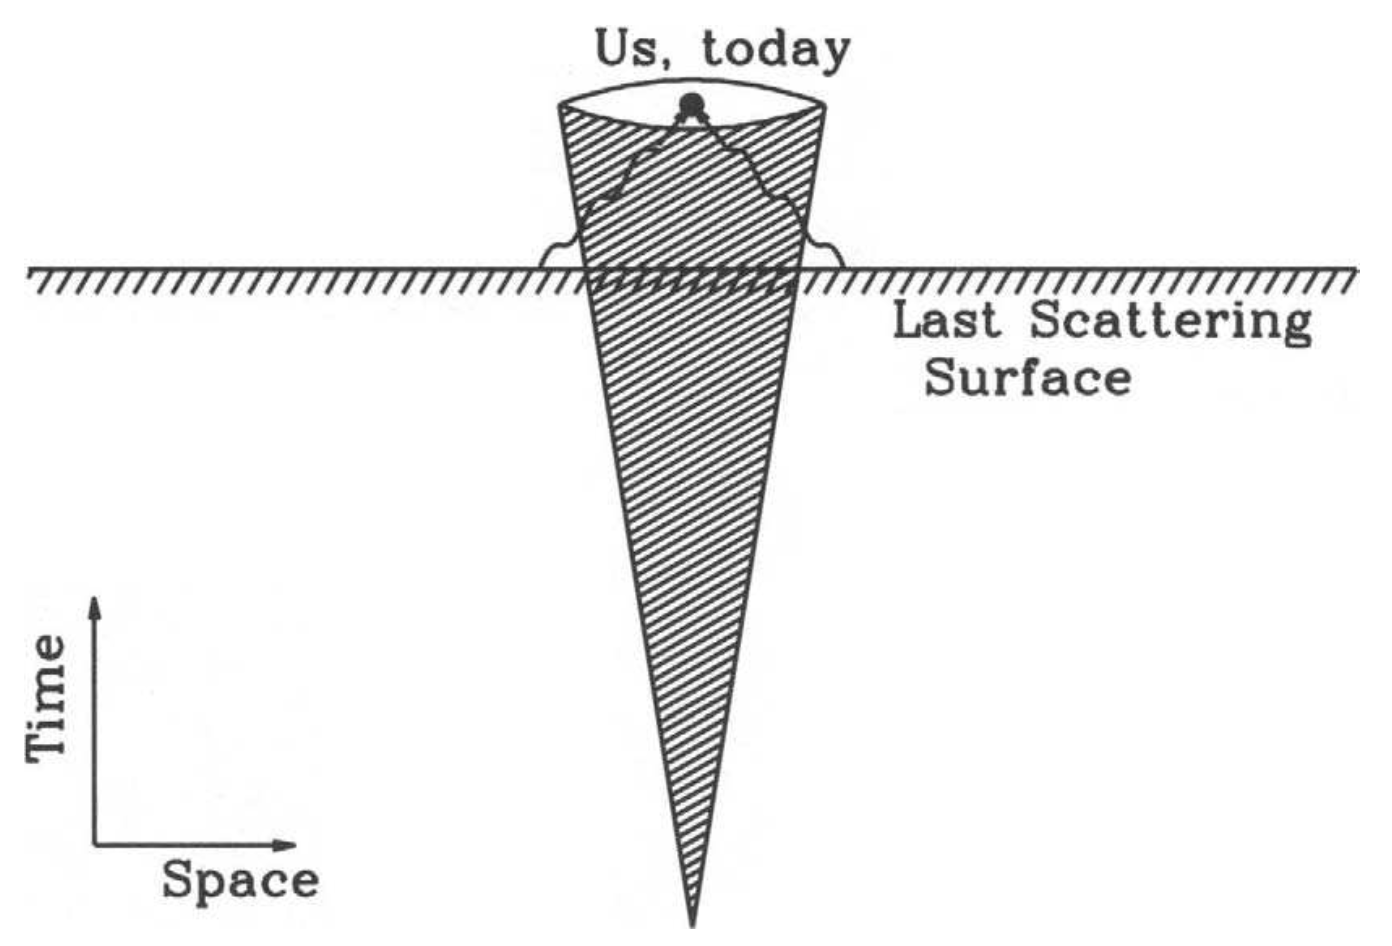
\includegraphics[width=8cm]{figures/cosmology/HorizonProblem.png}}
\end{figure}

\begin{align*}
    r_{H,{\rm prop}}(z_{\rm rec}) = 2\frac{c}{H_0} \Omega_m^{-1/2}(1+z_{\rm rec})^{-3/2} ~ [{\rm Mpc}]
\end{align*}

{\noindent}is the \textbf{horizon length at recombination}. We can then calculate the \textbf{angular size} on the sky that this length corresponds to,

\begin{align*}
    \theta_{H,{\rm rec}} = \frac{r_{H,{\rm prop}}(z_{\rm rec})}{D_A(z_{\rm rec})} ~ [{\rm rad}],
\end{align*}

{\noindent}where $D_A$ is the \textbf{angular diameter distance} to the last scattering surface of the CMB. Using the famous \textbf{Mattig relation} for $\Lambda=0$,

\begin{align*}
    D_A(z) = \frac{c}{H_0}\frac{2}{\Omega_m^2(1+z)^2} \left[ \Omega_mz+(\Omega_m-2)(\sqrt{1+\Omega_mz}-1) \right] ~ [{
    \rm Mpc}],
\end{align*}

{\noindent}we find that in the case of $\Omega_\Lambda=0$,

\begin{align*}
    D_A(z) \approx \frac{c}{H_0}\frac{2}{\Omega_mz} ~ [{\rm Mpc}] ~ {\rm for} ~ z\gg1,
\end{align*}

{\noindent}and hence,

\begin{align*}
    \theta_{\rm H,{\rm rec}} \approx \sqrt{\frac{\Omega_m}{z_{\rm rec}}} \sim \frac{\sqrt{\Omega_m}}{30} \sim \sqrt{\Omega_m} 2^\circ ~ {\rm for} ~ \Omega_\Lambda=0.
\end{align*}

{\noindent}This means that the horizon length at recombination subtends an angle of about $1^\circ$ on the sky.

{\noindent}Since no signal can travel faster than light, the existence of a horizon length means that CMB radiation from two directions separated by more than about one degree originates in regions that were not in causal contact before recombination, (i.e., the time when the CMB photons interacted with matter the last time). Therefore, these two regions have never been able to exchange information, for example about their temperature. Nevertheless their temperature is the same, as seen from the high degree of isotropy of the CMB, which shows relative fluctuations of only $\Delta T/T10^{-5}$!

{\noindent}During inflation, $H(a)=\sqrt{\Lambda/3}$ is constant so that the integral for the comoving horizon length formally diverges. This implies that the horizon may become arbitrarily large in the inflationary phase, depending on the duration of the exponential expansion. For illustration we consider a very small region in space of size $L<ct_i$ at a time $t_i\sim10^{-34}\,{\rm s}$ prior to inflation which is in causal contact. Through inflation, it expands tremendously, e.g., by a factor $10^{40}$; the original $L\sim10^{-24}\,{\rm cm}$ inflates to about $10^{16}\,{\rm cm}$ by the end of the inflationary phase, at $t_f\sim10^{-32}{\rm s}$. By today, this spatial region will have expanded by another factor of $10^{25}$ by following (for $t>t_f$) the normal cosmic expansion, to   $10^{41}\,{\rm cm}$. This scale is considerably larger than the size of the currently visible Universe, $c/H_0$. According to this scenario, the whole Universe visible today was in causal contact prior to inflation, so that the homogeneity of the physical conditions at recombination, and with it the nearly perfect isotropy of the CMB, is provided by causal processes.

{\noindent}\textbf{The flatness problem}: Due to the tremendous expansion, any initial curvature is straightened out -- For the total density parameter to be of order unity today, it must have been extremely close to $1$ at earlier times, which means that a very precise `fine tuning' of this parameter was necessary. Formally this can be seen as follows: during the inflationary phase we have

\begin{align*}
    \Omega_\Lambda = \frac{\Lambda}{3H^2} = 1 ~ [{\rm dimensionless}],
\end{align*}

{\noindent}and since it is assumed that the inflationary phase lasts long enough for the vacuum energy to be completely dominant, when it ends we then have $\Omega_0=1$. Hence the Universe is flat to an extremely good approximation.

{\noindent}The inflationary model of the very early Universe predicts that today $\Omega_0=1$ is valid to very high precision; any other value of $\Omega_0$ would require another fine-tuning. Thus our Universe is expected to be flat.

{\noindent}The physical details of the inflationary scenario are not very well known. In particular it is not yet understood how the phase transition at the end of the inflationary phase took place and why it did not occur earlier. But the two achievements presented above (and some others) make an inflationary phase appear a very plausible scenario. The inflationary model provides a natural, and in fact the only plausible, explanation for the origin of density fluctuations in the Universe which must have been present at very early epochs as the seeds of structure formation.

{\noindent}\textbf{The monopole problem}: The monopole problem -- that is, the apparent lack of magnetic monopoles in the Universe -- is not a purely cosmological problem, but one that results from combining the Hot Big Bang scenario with the particle physics concept of a Grand Unified Theory. In particle physics, a Grand Unified Theory, or GUT, is a field theory which attempts to unify the electromagnetic force, the weak nuclear force, and the strong nuclear force. Unification of forces has been a goal of scientists since the 1870s, when James Clerk Maxwell demonstrated that electricity and magnetism are both manifestations of a single underlying electromagnetic field. Currently, it is customary to speak of the four fundamental forces of nature: gravitational, electromagnetic, weak, and strong. In the view of many physicists, though, four forces are three too many; they've spent much time and effort to show that two or more of the ``fundamental forces'' are actually different aspects of a single underlying force. About a century after Maxwell, Steven Weinberg, Abdus Salam, and Sheldon Glashow successfully devised an electroweak theory. They demonstrated that at particle energies greater than $E\sim1\,{\rm TeV}$, the electromagnetic force and the weak force unite to form a single ``electroweak'' force. The electroweak energy of $E_\mathrm{ew}\sim1\,{\rm TeV}$ corresponds to a temperature $T_\mathrm{ew}\sim E_\mathrm{ew}/k_B\sim10^{16}\,{\rm K}$; the Universe had this temperature when its age was $t_\mathrm{ew}\sim10^{-12}\,{\rm s}$. Thus, when the Universe was less than a picosecond old, there were only three fundamental forces: the gravitational, strong, and electroweak force. When the predictions of the electroweak energy were confirmed experimentally, Weinberg, Salam, and Glashow toted home their Nobel Prizes, and physicists braced themselves for the next step: unifying the electroweak force with the strong force.

{\noindent}By extrapolating the known properties of the strong and electroweak forces to higher particle energies, physicists estimate that at an energy $E_\mathrm{GUT}$ of roughly $10^{12}-10^{13}\,{\rm TeV}$, the strong and electroweak forces should be unified as a single Grand Unified Force. If the GUT energy is $E_\mathrm{GUT}\sim10^{12}\,{\rm TeV}$, this corresponds to a temperature $T_\mathrm{GUT}\sim10^{28}\,{\rm K}$ and an age for the Universe of $t_\mathrm{GUT}\sim10^{-36}\,{\rm s}$. The GUT energy is about four orders of magnitude smaller than the Planck energy, $E_\mathrm{P}\sim10^{16}\,{\rm TeV}$. Physicists are searching for a Theory of Everything (TOE) which describes how the Grand Unified Force and the force of gravity ultimately unite to form a single unified force at the Planck scale. The different unification energy scales, and the corresponding temperatures and times in the early Universe, are shown in Figure \ref{fig:gut}.

\begin{figure}[h]
    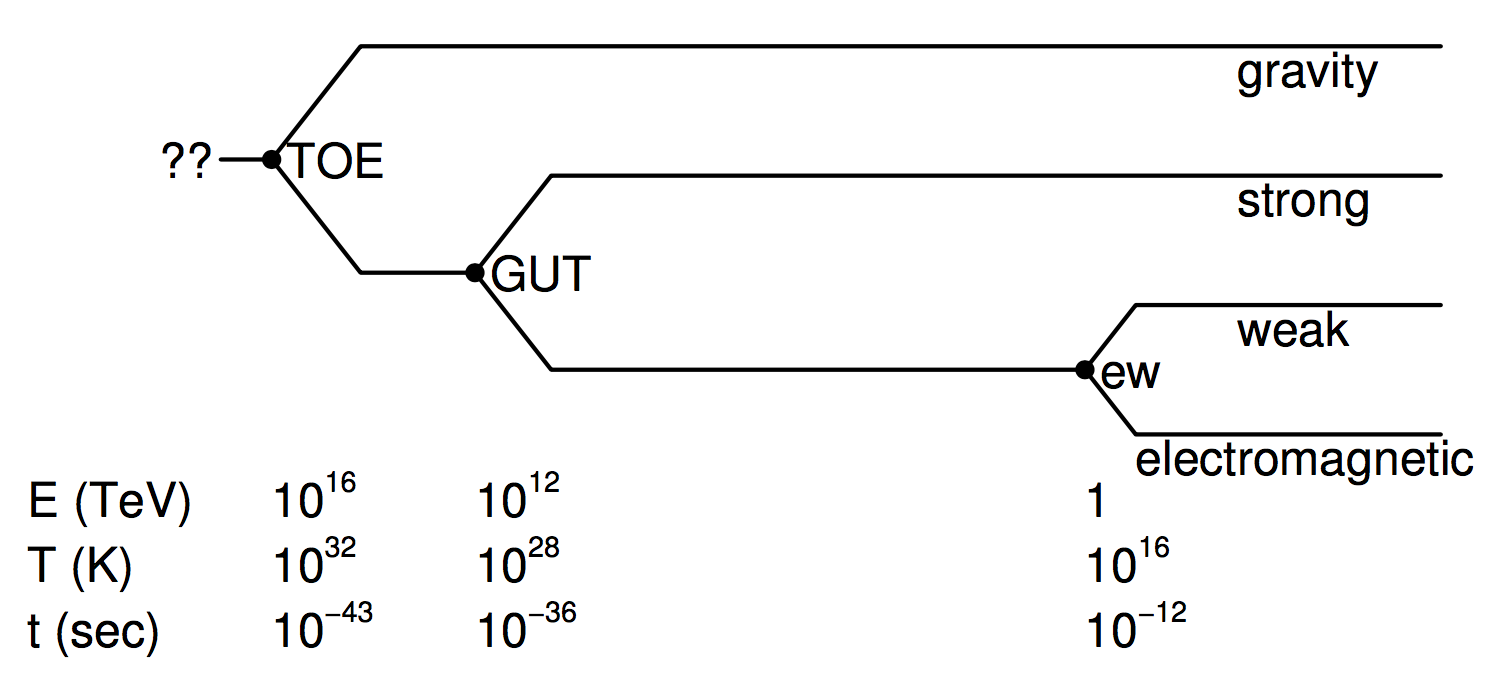
\includegraphics[width=14cm]{figures/cosmology/GUT.png}
    \centering
    \caption{\footnotesize{The energy, temperature, and time scales at which the different force unifications occur. Image taken from Ryden (2006).}}
    \label{fig:gut}
\end{figure}

{\noindent}One of the predictions of GUT is that the Universe underwent a phase transition as the temperature dropped below the GUT temperature. Generally speaking, phase transitions are associated with a spontaneous loss of symmetry as the temperature of a system is lowered. Take, as an example, the phase transition known as ``freezing water''. At temperatures $T>273\,{\rm K}$, water is liquid. Individual water molecules are randomly oriented, and the liquid water thus has rotational symmetry about any point; in other words, it is isotropic. However, when the temperature drops below $T=273\,{\rm K}$, the water undergoes a phase transition, from liquid to solid, and the rotational symmetry of the water is lost. The water molecules are locked into a crystalline structure, and the ice no longer has rotational symmetry about an arbitrary point. In other words, the ice crystal is anisotropic, with preferred directions corresponding to the crystal’s axes of symmetry. In a broadly similar vein, there is a loss of symmetry when the Universe undergoes the GUT phase transition at $t_\mathrm{GUT}\sim10^{-36}\,{\rm s}$. At $T>T_\mathrm{GUT}$, there was a symmetry between the strong and electroweak forces. At $T<T_\mathrm{GUT}$, the symmetry is spontaneously lost; the strong and electroweak forces begin to behave quite differently from each other.

{\noindent}In general, phase transitions associated with a loss of symmetry give rise to flaws known as topological defects. To see how topological defects form, consider a large tub of water which is cooled below $T=273\,{\rm K}$. Usually, the freezing of the water will start at two or more widely separated nucleation sites. The crystal which forms about any given nucleation site is very regular, with well-defined axes of symmetry. However, the axes of symmetry of two adjacent ice crystals will be misaligned. At the boundary of two adjacent crystals, there will be a two-dimensional topological defect, called a domain wall, where the axes of symmetry fail to line up. Other types of phase transitions give rise to one-dimensional, or line-like, topological defects (in a cosmological context, these linear defects are known as cosmic strings). Still other types of phase transitions give rise to zero-dimensional, or point-like, topological defects. GUT predict that the GUT phase transition creates point-like topological defects which act as magnetic monopoles. That is, they act as the isolated north pole or south pole of a magnet. The rest energy of the magnetic monopoles created in the GUT phase transition is predicted to be $m_Mc^2\sim E_\mathrm{GUT}\sim10^{12}\,{\rm TeV}$. This corresponds to a mass of over a nanogram (comparable to that of a bacterium), which is a lot of mass for a single particle to be carrying around. At the time of the GUT phase transition, points further apart than the horizon size will be out of causal contact with each other. Thus, we expect roughly one topological defect per horizon volume, due to the mismatch of fields which are not causally linked. The number density of magnetic monopoles, at the time of their creation, would be

\begin{align*}
    n_M(t_\mathrm{GUT}) \sim \frac{1}{(2ct_\mathrm{GUT})^3} \sim 10^{82} ~ [{\rm m^{-3}}],
\end{align*}

{\noindent}and their energy density would be

\begin{align*}
    (m_Mc^2)n_M \sim 10^{94}\,{[\rm TeV\,m^{-3}]}.
\end{align*}

{\noindent}This is a large energy density, but it is smaller by ten orders of magnitude than the energy density of radiation at the time of the GUT phase transition:

\begin{align*}
    \alpha T_\mathrm{GUT}^4 \sim 10^{104}\,{[\rm TeV\,m^{-3}]}.
\end{align*}

{\noindent}Thus, the magnetic monopoles wouldn't have kept the Universe from being radiation-dominated at the time of the GUT phase transition. However, the magnetic monopoles, being so massive, would soon have become highly non-relativistic, with energy density $\propto a^{-3}$. The energy density in radiation, though, was falling off at the rate $\propto a^{-4}$. Thus, the magnetic monopoles would have dominated the energy density of the Universe when the scale factor had grown by a factor $\sim10^{10}$; that is, when the temperature had fallen to $T\sim10^{-10}\,T_\mathrm{GUT}\sim10^{18}\,{\rm K}$, and the age of the Universe was only $t\sim10^{-16}\,{\rm s}$.

{\noindent}Obviously, the Universe is not dominated by magnetic monopoles today. In fact, there is no strong evidence that they exist at all. Every north magnetic pole which we can find is paired with a south magnetic pole, and vice versa. There are no isolated north poles or isolated south poles. The monopole problem can thus be rephrased as the question, ``Where have all the magnetic monopoles gone?'' Now, you can always answer the question, ``Where have the monopoles gone?'' by saying, ``There were never any monopoles to begin with''” There is not yet a single, definitive GUT, and in some variants on the GUT theme, magnetic monopoles are not produced. However, the flatness and horizon problems are not so readily dismissed. When the physicist Alan Guth first proposed the idea of inflation in 1981, he introduced it as a way of resolving the flatness problem, the horizon problem, and the monopole problem with a single cosmological mechanism.

\subsubsection{Follow-up Questions}

\begin{itemize}
    \item Can you calculate/give an estimate or back-of-the-envelope idea of how flat the Universe would have been after inflation if today it was say 1\% non-flat?
    \item What physically causes inflation?
    \item Why, physically, does having an inflaton result in inflation? What physically happens?
    \item Is inflation the only way to explain these observations?

\end{itemize}

% --------------------------------------------------------------
%
%                           12. 
%
% --------------------------------------------------------------

\newpage
\subsection{Question 12}

Define and describe a `fine tuning problem'. How do anthropic arguments attempt to resolve it?

\subsubsection{Short answer}

The flatness problem: for the total density parameter to be of order unity today, it must have been extremely close to $1$ at earlier times, which means that a very precise `fine tuning' of this parameter was necessary. By anthropic arguments, we live in a Universe which had, at a very early time, a very precisely tuned density parameter, because only in such a Universe can life evolve and astronomers exist to examine the flatness of the Universe. In all other conceivable Universes this would not be possible. This approach is meaningful only if a large number of Universes existed—in this case we should not be too surprised about living in one of those where this initial fine-tuning took place—in the other ones, we, and the question about the cosmological parameters, would just not exist. This approach is called the \textbf{anthropic principle}.

\subsubsection{Additional context}

Let us consider the consequences of the case where $\Omega_0$ had not been so extremely close to $1$ at $z\sim10^{10}$; then, the Universe would have recollapsed long ago, or it would have expanded significantly faster than the Universe we live in. In either case, the consequences for the evolution of life in the Universe would have been catastrophic. In the first case, the total lifetime of the Universe would have been much shorter than is needed for the formation of the first stars and the first planetary systems, so that in such a world no life could be formed. In the second case, extreme expansion would have prevented the formation of structure in the Universe. In such a Universe no life could have evolved either. 

{\noindent}This consideration can be interpreted as follows: we live in a Universe which had, at a very early time, a very precisely tuned density parameter, because only in such a Universe can life evolve and astronomers exist to examine the flatness of the Universe. In all other conceivable Universes this would not be possible. This approach is meaningful only if a large number of Universes existed (in this case we should not be too surprised about living in one of those where this initial fine-tuning took place) in the other ones, we, and the question about the cosmological parameters, would just not exist. This approach is called the anthropic principle. It may either be seen as an `explanation' for the flatness of our Universe, or as a capitulation -- where we give up to explore a physical reason for the origin of the flatness of our Universe.

\subsubsection{Follow-up Questions}

\begin{itemize}
    \item What are other fine tuning problems? (Note: if you talk about $\Omega_k$, you cannot talk about $\Omega_\Lambda$ since they are related.)
    \item How do you \textit{feel} about the anthropic principle?
    \item Is the anthropic principle a scientifically or logically sound argument?
    \item What is the weak versus strong anthropic principle?
\end{itemize}


% --------------------------------------------------------------
%
%                           13. 
%
% --------------------------------------------------------------

\newpage
\subsection{Question 13}

Define the two-point correlation function. How is it related to the power spectrum? How is the $C_\ell$ spectrum of the CMB related to low redshift galaxy clustering?

\subsubsection{Short answer}

The \textbf{two-point correlation function} is given by

\begin{align*}
    \xi_g(r) = \left(\frac{r}{r_0}\right)^{-\gamma} ~ [{\rm dimensionless}],
\end{align*}

{\noindent}where $r_0\sim5\,h^{-1}\,{\rm Mpc}$ denotes the correlation length, and the slope is about $\gamma\simeq1.7$. It is related to the \textbf{power spectrum} $P(k)$ via the Fourier transform

\begin{align*}
    P(k) = 2\pi \int\limits_0^\infty x^2\frac{\sin(kx)}{kx}\xi(x)\mathrm{d}x ~ [{\rm dimensionless}].
\end{align*}

\subsubsection{Additional context}

Galaxies are not randomly distributed in space, but rather they gather in groups, clusters, or even larger structures. Phrased differently, this means that the probability of finding a galaxy at location x is not independent of whether there is a galaxy at a neighboring point y. It is more probable to find a galaxy in the vicinity of another one than at an arbitrary location. This phenomenon is described such that one considers two points $\mathbf{x}$ and $\mathbf{y}$, and two volume elements $\mathrm{d}V$ around these points. If $\bar{n}$ is the average number density of galaxies, the probability of finding a galaxy in the volume element $\mathrm{d}V$ around $x$ is then

\begin{align*}
    P_1 = \bar{n}\mathrm{d}V ~ [{\rm dimensionless}],
\end{align*}

{\noindent}independent of $\mathbf{x}$ if we assume that the Universe is statistically homogeneous. We choose $\mathrm{d}V$ such that $P_1\ll1$, so that the probability of finding two or more galaxies in this volume element is negligible.

{\noindent}The probability of finding a galaxy in the volume element $\mathrm{d}V$ at location $\mathbf{x}$ and at the same time finding a galaxy in the volume element $\mathrm{d}V$ at location $\mathbf{y}$ is then

\begin{align*}
    P_2 = (\bar{n}\mathrm{d}V)^2 [1+\xi_g(\mathbf{x},\mathbf{y})] ~ [{\rm dimensionless}].
\end{align*}

{\noindent}If the distribution of galaxies was uncorrelated, the probability $P_2$ would simply be the product of the probabilities of finding a galaxy at each of the locations $\mathbf{x}$ and $\mathbf{y}$ in a volume element $\mathrm{d}V$, so $P_2=P_1^2$. But since the distribution is correlated, the relation does not apply in this simple form; rather, it needs to be modified, as was done. This equation defines the \textbf{two-point correlation function} (or simply `\textbf{correlation function}') of galaxies $\xi_g(\mathbf{x},\mathbf{y})$.

{\noindent}By analogy to this, the correlation function for the total matter density can be defined as

\begin{align*}
    \langle\rho(\mathbf{x})\rho(\mathbf{y})\rangle &= \bar{\rho}^2\langle[1+\delta(\mathbf{x})][1+\delta(\mathbf{y})]\rangle \\
    &= \bar{\rho}^2 (1+\delta(\mathbf{x})\delta(\mathbf{y})) \\
    &= \bar{\rho}^2(1+\xi(\mathbf{x},\mathbf{y})) ~ [{\rm dimensionless}],
\end{align*}

{\noindent}because the mean (or expectation) value $\langle\delta(\mathbf{x})\rangle$ for all locations $\mathbf{x}$.

{\noindent}In the above equations, angular brackets denote averaging over an ensemble of distributions that all have identical statistical properties. In our example of the lake, the correlation function of the wave amplitudes at positions $\mathbf{x}$ and $\mathbf{y}$, for instance, would be determined by taking a large number of snapshots of its surface and then averaging the product of the amplitudes at these two locations over all these realizations.

{\noindent}Since the Universe is considered statistically homogeneous, $\xi$ can only depend on the difference $\mathbf{x}-\mathbf{y}$ and not on $\mathbf{x}$ and $\mathbf{y}$ individually. Furthermore, $\xi$ can only depend on the separation $r=\lvert\mathbf{x}-\mathbf{y}\rvert$, and not on the direction of the separation vector $\mathbf{x}-\mathbf{y}$ because of the assumed statistical isotropy of the Universe. Therefore, $\xi=\xi(r)$ is simply a function of the separation between two points.

{\noindent}For a homogeneous random field, the ensemble average can be replaced by spatial averaging (i.e., the correlation function can be determined by averaging over the products of densities at pairs of points) for a large number of pairs of points with given separation $r$. For determining the correlation function of galaxies, we note that $\xi_g(r)$ is the excess probability to find a galaxy at a separation $r$ from another galaxy, relative to that of a random distribution. Therefore, $\xi_g(r)$ can be determined by first counting the number of galaxy pairs with separation in the interval $\Delta r$ around $r$. Then one creates a random distribution of the same number of objects in the same volume, and again counts the pairs in the same distance interval. The ratio of these two pair counts then yields an estimate for $\xi_g(r)$.

{\noindent}The equivalence of ensemble average and spatial average is called the ergodicity of the random field. Only by this can the correlation function (and all other statistical properties) in our Universe be measured at all, because we are able to observe only a single (namely our) realization of the hypothetical ensemble. From the measured correlations between galaxy positions, as determined from spectroscopic redshift surveys of galaxies, one finds the approximate relation

\begin{align*}
    \xi_g(r) = \left(\frac{r}{r_0}\right)^{-\gamma} ~ [{\rm dimensionless}],
\end{align*}

{\noindent}for galaxies of luminosity $\sim L^*$, where $r_0\sim5\,h^{-1}\,{\rm Mpc}$ denotes the correlation length, and where the slope is about $\gamma\simeq1.7$. This relation is approximately valid over a range of separations $0.2h^{-1}\,{\rm Mpc}\lesssim r \lesssim 30h^{-1}\,{\rm Mpc}$.

{\noindent}Hence, the correlation function provides a means to characterize the structure of the cosmological matter distribution. Besides this two-point correlation function, correlations of higher order may also be defined, leading to general n-point correlation functions. These are more difficult to determine from observation, though. It can be shown that the statistical properties of a random field are fully specified by the set of all n-point correlations.

{\noindent}An alternative (and equivalent) description of the statistical properties of a random field, and thus of the matter distribution in a Universe, is the power spectrum $P(k)$. Roughly speaking, the power spectrum $P(k)$ describes the level of structure as a function of the length-scale $L\simeq2\pi/k$; the larger $P(k)$, the larger the amplitude of the fluctuations on a length-scale $2\pi/k$. Here, $k$ is a comoving wave number. Phrased differently, the density fluctuations are decomposed into a sum of plane waves of the form $\delta(\mathbf{x})=\sum a_k\cos(\mathbf{x}\cdot\mathbf{k})$, with a wave vector $\mathbf{k}$ and an amplitude $a_k$. The power spectrum $P(k)$ then describes the mean of the squares, $\lvert a_k\rvert^2$, of the amplitudes, averaged over all wave vectors with equal length $k=\lvert\mathbf{k}\lvert$. Technically speaking, this is a Fourier decomposition. Referring back to the example of waves on the surface of a lake, one finds that a characteristic wavelength $L_c$ exists, which depends, among other factors, on the wind speed. In this case, the power spectrum will have a prominent maximum at $k=2\pi/L_c$.

{\noindent}The power spectrum $P(k)$ and the correlation function are related through a Fourier transform; formally, one has

\begin{align*}
    P(k) = 2\pi \int\limits_0^\infty x^2\frac{\sin(kx)}{kx}\xi(x)\mathrm{d}x ~ [{\rm dimensionless}],
\end{align*}

{\noindent}i.e., the integral over the correlation function with a weight factor depending on $k\sim2\pi/L$. This relation can also be inverted, and thus $\xi(x)$ can be computed from $P(k)$.

{\noindent}Since the CMB temperature fluctuations $\delta T/T$ is defined on the surface of a sphere -- the celestial sphere, in this case -- it is useful to expand it in spherical harmonics:

\begin{align*}
    \frac{\delta T}{T}(\theta,\phi) = \sum\limits_{\ell=0}^{\infty}\sum\limits_{m=-1}^{\ell} a_{\ell m}Y_{\ell m}(\theta,\phi)
\end{align*}

{\noindent}where $Y_{\ell m}(\theta,\phi)$ are the usual \textbf{spherical harmonic functions}\footnote{\href{https://en.wikipedia.org/wiki/Table\_of\_spherical\_harmonics}{https://en.wikipedia.org/wiki/Table\_of\_spherical\_harmonics}}. What concerns cosmologists is not the exact pattern of hot spots and cold spots on the sky, but their statistical properties. The most important statistical property of $\delta T/T$ is the correlation function $C(\theta)$. Consider two points on the last scattering surface. Relative to an observer, they are in the directions $\hat{n}$ and $\hat{n}'$, and are separated by an angle $\theta$ given by the relation $cos\theta=\hat{n}\cdot\hat{n}'$. To find the correlation function $C(\theta)$, multiply together the values of $\delta T/T$ at the two points, then average the product over all points separated by the angle $\theta$:

\begin{align*}
    C(\theta) = \left\langle\frac{\delta T}{T}(\hat{n})\frac{\delta T}{T}(\hat{n}')\right\rangle_{\hat{n}\cdot\hat{n}'=\cos\theta}
\end{align*}

{\noindent}If cosmologists knew the precise value of $C(\theta)$ for all angles from $\theta=0$ to $\theta=180^\circ$, they would have a complete statistical description of the temperature fluctuations over all angular scales. Unfortunately, the CMB measurements which tell us about $C(\theta)$ contain information over only a limited range of angular scales.

{\noindent}The limited angular resolution of available observations is what makes the spherical harmonic expansion of $\delta T/T$ so useful. Using the expansion of $\delta T/T$ in spherical harmonics, the correlation function can be written in the form

\begin{align*}
    C(\theta) = \frac{1}{4\pi} \sum\limits_{\ell=0}^\infty (2\ell+\ell)(C_\ell)P_\ell(cos\theta),
\end{align*}

{\noindent}where $P_\ell$ are the usual \textbf{Legendre polynomials}:

\begin{align*}
    P_0(x) = 1 \\
    P_1(x) = x \\
    P_2(x) = \frac{1}{2}(3x^2-1)
\end{align*}

{\noindent}and so forth. In this way, a measured correlation function $C(\theta)$ can be broken down into its multipole moments $C_\ell$.

{\noindent}Generally speaking, a term $C_\ell$ is a measure of temperature fluctuations on the angular scale $\theta\sim180^\circ/\ell$. Thus, the multipole $\ell$ is interchangeable, for all practical purposes, with the angular scale $\theta$. The $\ell=0$ (monopole) term of the correlation function vanishes if you've defined the mean temperature correctly. The $\ell=1$ (dipole) term results primarily from the Doppler shift due to our motion through space. It is the moments with $\ell\geq2$ which are of the most interest to cosmologists, since they tell us about the fluctuations present at the time of last scattering.

{\noindent}In presenting the results of CMB observations, it is customary to plot the function

\begin{align*}
    \Delta T \equiv \sqrt{\frac{\ell(\ell+1)}{2\pi}}\langle T \rangle ~ [{\rm K}],
\end{align*}

{\noindent}since this function tells us the contribution per logarithmic interval in $\ell$ to the total temperature fluctuation $\delta T$ of the CMB. The detailed shape of the $\Delta T$ versus $\ell$ curve contains a wealth of information about the Universe at the time of photon decoupling. 

{\noindent}At the time of last scattering, a particularly interesting length scale, cosmologically speaking, is the Hubble distance,

\begin{align*}
    d_H = \frac{c}{H(z_\mathrm{ls})} \approx \frac{3\times10^8\,{\rm m\,s^{-1}}}{1.24\times10^{-18}\,s^{-1}(1101)^{3/2}} \approx 6.6\times10^{21}\,{\rm m} \approx 0.2\,{[\rm Mpc]},
\end{align*}

{\noindent}where the redshift of last scattering is $z_\mathrm{ls}\approx1100$. A patch of the last scattering surface with this physical size will have an angular size, as seen from Earth, of

\begin{align*}
    \theta_H = \frac{c/H(z_\mathrm{ls})}{d_A} \approx \frac{0.2\,{\rm Mpc}}{13\,{\rm Mpc}} \approx 0.015\,{\rm rad} \approx 1^\circ.
\end{align*}

{\noindent}It is no coincidence that the peak in the $\Delta T$ versus $\ell$ curve occurs at an angular scale $Ξ\sim\theta_H$. The origin of temperature fluctuations with $\theta>\theta_H$ ($\ell<180$) is different from those with $\theta<\theta_H$ ($\ell>180$).


% --------------------------------------------------------------
%
%                           14. 
%
% --------------------------------------------------------------

\newpage
\subsection{Question 14}

Consider a cosmological model including a positive cosmological constant. Show that, in such a model, the expansion factor eventually expands at an exponential rate. Sketch the time dependence of the expansion factor in the currently favoured cosmological model.

\subsubsection{Short answer}

{\noindent}Friedmann equation can be written in terms of $\Omega_{r,0}$, $\Omega_{m,0}$, and $\Omega_{\Lambda,0}$ via

\begin{align*}
    \left(\frac{H}{H_0}\right)^2 = \frac{\Omega_{r,0}}{a^4} + \frac{\Omega_{m,0}}{a^3} + \Omega_{\Lambda,0} + \frac{1-\Omega_0}{a^2}
\end{align*}

{\noindent}where $\Omega_0=\Omega_{r,0}+\Omega_{m,0}+\Omega_{\Lambda,0}$. Since $(H/H_0)^2=(\dot{a}/a)^2$, this can be re-written as

\begin{align*}
    \left(\frac{\dot{a}(t)}{a(t)}\right)^2 &= \frac{\Omega_{r,0}}{a^4} + \frac{\Omega_{m,0}}{a^3} + \Omega_{\Lambda,0} + \frac{1-\Omega_0}{a^2} \\
    \dot{a}(t) &= a(t)\sqrt{\frac{\Omega_{r,0}}{a^4} + \frac{\Omega_{m,0}}{a^3} + \Omega_{\Lambda,0} + \frac{1-\Omega_0}{a^2}}.
\end{align*}

{\noindent}For $a\gg1$, this simplifies to

\begin{align*}
    \frac{\mathrm{d}a}{\mathrm{d}t} &\approx a(t)\sqrt{\Omega_{\Lambda,0}} \\
    a(t) &\approx e^{\sqrt{\Omega_{\Lambda,0}}t}.
\end{align*}

{\noindent}Therefore, at large scale factors, the expansion proceeds at the exponential rate as follows:

\begin{align*}
    a(t) \propto e^{\sqrt{\Omega_{\Lambda,0}}t}.
\end{align*}

{\noindent}Figure \ref{fig:avst} shows the time-dependence of the scale factor $a(t)$ in the Benchmark Model.

\begin{figure}[h]
    \floatbox[{\capbeside\thisfloatsetup{capbesideposition={right,top},capbesidewidth=4cm}}]{figure}[\FBwidth]
    {\caption{\footnotesize{The scale factor $a$ as a function of time $t$ (measured in units of the Hubble time), computed for the Benchmark Model. The dotted lines indicate the time of radiation-matter equality, $a_{rm}=2.8\times10^{-4}$, the time of matter-lambda equality, $a{m\Lambda}=0.75$, and the present moment, $a_0=1$. Figure taken from Ryden (2006).}}
    \label{fig:avst}}
    {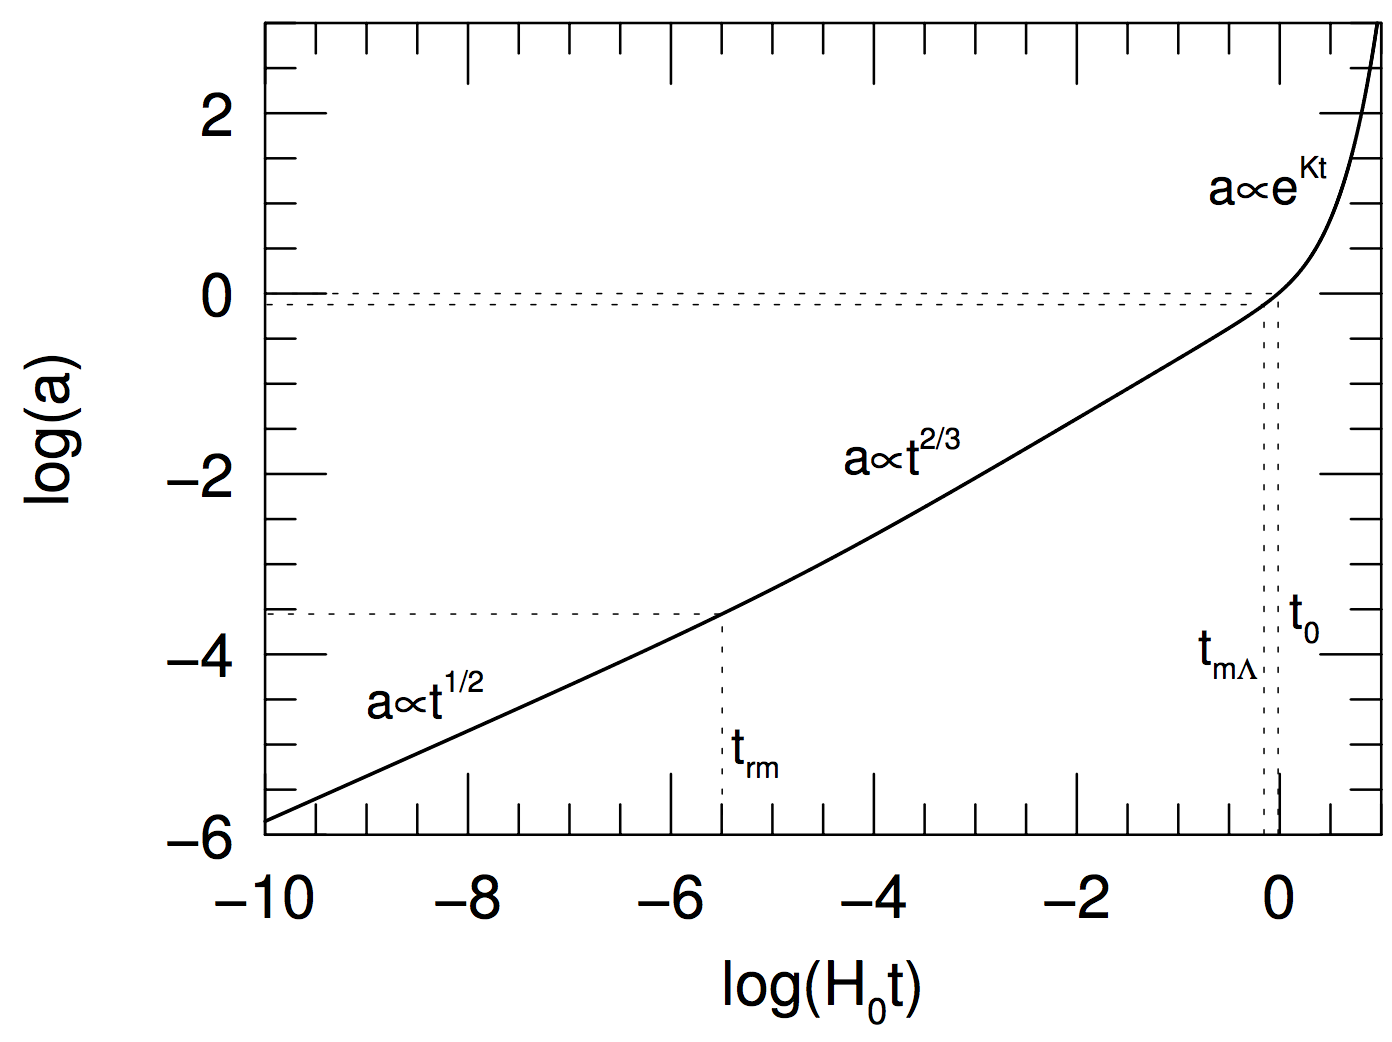
\includegraphics[width=10cm]{figures/cosmology/avst.png}}
\end{figure}

\subsubsection{Additional context}

{\noindent}The Benchmark Model, is adopted as the best fit to the currently available observational data, is spatially flat, and contains radiation, matter, and a cosmological constant. The Hubble constant of the Benchmark Model is assumed to be $H_0=70\,{\rm km\,s^{-1}\,Mpc^{-1}}$. The radiation in the Benchmark Model consists of photons and neutrinos. The photons are assumed to be provided solely by a CMB with current temperature $T_0=2.725\,{\rm K}$ and density parameter $\Omega_{\gamma,0}=5.0\times10^{-5}$. The energy density of the CNB is theoretically calculated to be 68\% of that of the CMB, as long as neutrinos are relativistic. If a neutrino has a non-zero mass $m_\nu$, it defects from the ``radiation'' column to the ``matter'' column when the scale factor is $a\sim5\times10^{-4}\,{\rm eV}/(m_\nu c^2)$. The matter content of the Benchmark Model consists partly of baryonic matter (that is, matter composed of protons and neutrons, with associated electrons), and partly of nonbaryonic dark matter; the evidence indicates that most of the matter in the Universe is nonbaryonic dark matter. The baryonic material that we are familiar with from our everyday existence has a density parameter of $\Omega_{b,0}\approx0.04$ today. The density parameter of the nonbaryonic dark matter is roughly six times greater: $\Omega_{c,0}\approx0.26$. The bulk of the energy density in the Benchmark Model, however, is not provided by radiation or matter, but by a cosmological constant, with $\Omega_{\Lambda,0}=1-\Omega_{m,0}-\Omega_{r,0}\approx0.70$.

{\noindent}The Benchmark Model was first radiation-dominated, then matter-dominated, and is now entering into its lambda-dominated phase. Radiation gave way to matter at a scale factor $a_{rm}=\Omega_{r,0}/\Omega{m,0}=2.8\times10^{-4}$, corresponding to a time $t_{rm}=4.7\times10^4\,{\rm yr}$. Matter, in turn, gave way to the cosmological constant at $a_{m\Lambda}=(\Omega_{m,0}/\Omega_{\Lambda,0})^{1/3}$ corresponding to $t_{m\Lambda}=9.8\,{\rm Gyr}$. The current age of the Universe, in the Benchmark Model, is $t_0=13.5\,{\rm Gyr}$.

{\noindent}Figure \ref{fig:avst} shows the scale factor, thus computed, for the Benchmark Model. Note that the transition from the $a\propto t^{1/2}$ radiation-dominated phase to the $a\propto t^{2/3}$ matter-dominated phase is not an abrupt one; neither is the later transition from the matter-dominated phase to the exponentially growing lambda-dominated phase. One curious feature of the Benchmark Model which Figure \ref{fig:avst} illustrates vividly is that we are living very close to the time of matter-lambda equality.

{\noindent}\textbf{Radiation-Matter equality}: To find the redshift of radiation-matter equality, obtain the Friedmann equation for each component using the scale factor relations above along with the definition of the density parameter $\Omega \equiv \rho/\rho_c = (8{\pi}G/3H_0)\rho$. For the radiation component, this gives us:

\begin{equation*}
\begin{split}
\left(\frac{\dot{a}}{a}\right)^2 = \frac{8{\pi}G}{3}\rho_r(a)
\left(\frac{\dot{a}}{a}\right)^2 = \frac{8{\pi}G}{3}\rho_ra^{-4}
\left(\frac{\dot{a}}{a}\right)^2 = \frac{8{\pi}G}{3}\left(\frac{3H_0}{8{\pi}G}\Omega_r\right)a^{-4}
\left(\frac{\dot{a}}{a}\right)^2 = H_0\Omega_ra^{-4}
\end{split}
\end{equation*}

{\noindent}along with the following for the matter component:

\begin{equation*}
\begin{split}
\left(\frac{\dot{a}}{a}\right)^2 = \frac{8{\pi}G}{3}\rho_m(a)
\left(\frac{\dot{a}}{a}\right)^2 = \frac{8{\pi}G}{3}\rho_ma^{-3}
\left(\frac{\dot{a}}{a}\right)^2 = \frac{8{\pi}G}{3}\left(\frac{3H_0}{8{\pi}G}\Omega_m\right)a^{-3}
\left(\frac{\dot{a}}{a}\right)^2 = H_0\Omega_ma^{-3}.
\end{split}
\end{equation*}

{\noindent}Equating the two Friedmann equations and solving for the radiation-matter equality scale factor $a_{rm}$ using the relationship $a_{rm} = (1+z_{rm})^{-1}$ for redshift:

\begin{equation*}
\begin{split}
H_0\Omega_ra_{rm}^{-4} &= H_0\Omega_ma_{rm}^{-3} \\
\Omega_ra_{rm}^{-1} &= \Omega_ma_{rm}^{-1} \\
a_{rm} &= \frac{\Omega_r}{\Omega_m} \\
(z_{rm}+1)^{-1} &= \frac{\Omega_r}{\Omega_m} \\
(z_{rm}+1) &= \frac{\Omega_m}{\Omega_r} \\
z_{rm} &= \frac{\Omega_m}{\Omega_r} - 1 \\
z_{rm} &= \frac{0.27}{5\times10^{-5}} - 1 \\
z_{rm} &= 5399.
\end{split}
\end{equation*}

{\noindent}\textbf{Matter-$\Lambda$ equality}: To find the redshift of matter-$\Lambda$ equality, obtain the Friedmann equation for each component using the scale factor relations above along with the definition of the density parameter $\Omega \equiv \rho/\rho_c = (8{\pi}G/3H_0)\rho$. We already have the following for the matter component:

\begin{align*}
\left(\frac{\dot{a}}{a}\right)^2 = H_0\Omega_ma^{-3}
\end{align*}

{\noindent}so let's work it out for the $\Lambda$ component:

\begin{equation*}
\begin{split}
\left(\frac{\dot{a}}{a}\right)^2 = \frac{8{\pi}G}{3}\rho_\Lambda(a)
\left(\frac{\dot{a}}{a}\right)^2 = \frac{8{\pi}G}{3}\rho_\Lambda
\left(\frac{\dot{a}}{a}\right)^2 = \frac{8{\pi}G}{3}\left(\frac{3H_0}{8{\pi}G}\Omega_\Lambda\right)
\left(\frac{\dot{a}}{a}\right)^2 = H_0\Omega_\Lambda.
\end{split}
\end{equation*}

{\noindent}Equating the two Friedmann equations and solving for the matter-$\Lambda$ equality scale factor $a_{m\Lambda}$ using the relationship $a_{m\Lambda} = (1+z_{m\Lambda})^{-1}$ for redshift:

\begin{equation*}
\begin{split}
H_0\Omega_ma_{m\Lambda}^{-3} &= H_0\Omega_\Lambda \\
a_{m\Lambda}^{-3}& = \frac{\Omega_\Lambda}{\Omega_m} \\
a_{m\Lambda}^{3} &= \frac{\Omega_m}{\Omega_\Lambda} \\
\left[(1+z_{m\Lambda})^{-1}\right]^{3} &= \frac{\Omega_m}{\Omega_\Lambda} \\
(1+z_{m\Lambda})^{-3} &= \frac{\Omega_m}{\Omega_\Lambda} \\
(1+z_{m\Lambda}) &= \left(\frac{\Omega_m}{\Omega_\Lambda}\right)^{1/3} \\
z_{m\Lambda} &= \left(\frac{\Omega_m}{\Omega_\Lambda}\right)^{1/3} - 1 \\
z_{m\Lambda} &= \left(\frac{0.27}{0.73}\right)^{1/3} - 1 \\
z_{m\Lambda} &= 0.39.
\end{split}
\end{equation*}

\subsubsection{Follow-up Questions}

\begin{itemize}
    \item At what time/scalefactor/redshift did the radiation-matter equality take place?
    \item At what time/scalefactor/redshift did the matter-$\Lambda$ equality take place?
    \item What are the possible fates of the Universe?
\end{itemize}

% --------------------------------------------------------------
%
%                           15. 
%
% --------------------------------------------------------------

\newpage
\subsection{Question 15}

Define and describe the epoch of reionization. What are the observational constraints on it?

\subsubsection{Short answer}

After recombination occurring at a redshift $z\sim1,100$, the Universe entered the cosmic \textbf{Dark Ages} where it became predominantly neutral until $z\sim16$. Around this time, gravitational Jeans instabilities allowed for the formation of the first generation of stars. While they have yet to be directly observed, these Population III (Pop III) stars were particular massive ($\sim100\,M_\odot$), implying that they were extremely hot and capable of radiating significant amounts of ionizing UV photons. These Pop III stars triggered a significant phase transition in the IGM as they began ionizing the predominantly neutral gas during a time called the \textit{Epoch of Reionization} (EoR). There are several observational constraints on this period, including Ly$\alpha$ forest lines, Gunn-Peterson absorption, and CMB polarization.


\subsubsection{Additional context}

{\noindent}The baryonic pre-galactic medium (PGM) evolves in three distinct phases. At high redshifts ($z>1100$) the PGM is hot, fully ionized, and optically thick to \textbf{Thomson scattering}, and hence coupled to the photon field. As the Universe expands, the PGM cools, and eventually recombines, leaving a surface of last scattering (the CMB), plus a neutral PGM. This neutral phase lasts from $z=1100$ to $z\sim14$. At some point between $z\sim14$ and $6$, hydrogen in the PGM is ``reionized,'' due to UV radiation from the first luminous objects, leaving the fully reionized IGM seen during the ``realm of the galaxies'' ($0<z<6$). The ionized, dense PGM at very high redshift has been well studied through extensive observations of the CMB. Likewise, the reionized, rarified IGM at low redshift has been well characterized through QSO absorption line studies. The middle phase (the existence of a neutral IGM during the so-called dark ages and the process of reionization of this medium) is the last directly observable phase of cosmic evolution that remains to be verified and explored. The epoch of reionization (EoR) is crucial in cosmic structure formation studies, because it sets a fundamental benchmark indicating the formation of the first luminous objects, either star-forming galaxies or active galactic nuclei (AGN).

{\noindent}After recombination at $z\sim1100$, the intergalactic gas became neutral, with a residual ionization fraction of only $10^{-4}$. Had the Universe remained neutral we would not be able to receive any photons that were emitted bluewards of the Ly$\alpha$ line of a source, because the absorption cross section for Ly$\alpha$ photons is too large. Since such photons are observed from QSOs, as can be seen for instance in the spectra of the $z>5.7$ QSOs in Figure \ref{fig:qsoabsorption}, and since an appreciable fraction of homogeneously distributed neutral gas in the intergalactic medium can be excluded for $z\gtrsim5$, from the tight upper bounds on the strength of the Gunn-Peterson effect, the Universe must have been reionized between the recombination epoch and the redshift $z\sim7$ of the most distant known QSOs.

{\noindent}This raises the question of how this reionization proceeded, in particular which process was responsible for it. The latter question is easy to answer -- reionization must have happened by photoionization. Collisional ionization can be ruled out because for it to be efficient the intergalactic medium (IGM) would need to be very hot, a scenario which can be excluded due to the perfect Planck spectrum of the CMB. Hence, the next question is what produced the energetic photons that caused the photoionization of the IGM.

{\noindent}Two kinds of sources may in principle account for them -- hot stars or AGNs. Currently, it is not unambiguously clear which of these is the predominant source of energetic photons causing reionization since our current understanding of the formation of supermassive black holes is still insufficient. However, it is currently thought that the main source of photoionization photons is the first generation of hot stars.

{\noindent}Following on from the above arguments, understanding reionization is thus directly linked to studying the first generation of stars. In the present Universe star formation occurs in galaxies; thus, one needs to examine when the first galaxies could have formed. From the theory of structure formation, the mass spectrum of dark matter halos at a given redshift can be computed by means of, e.g., the Press-Schechter model. Two conditions need to be fulfilled for stars to form in these halos. First, gas needs to be able to fall into the dark halos. Since the gas has a finite temperature, pressure forces may impede the infall into the potential well. Second, this gas also needs to be able to cool, condensing into clouds in which stars can then be formed.

{\noindent}By means of a simple argument, we can estimate under which conditions pressure forces are unable to prevent the infall of gas into a potential well. To do this, we consider a slightly overdense spherical region of radius $R$ whose density is only a little larger than the mean cosmic matter density $\bar{\rho}$. If this sphere is homogeneously filled with baryons, the gravitational binding energy of the gas is about

\begin{align*}
    \lvert E_\mathrm{pot} \rvert \sim \frac{GMM_g}{R} ~ [{\rm J}],
\end{align*}

{\noindent}where $M$ and $M_g$ denote the total mass and the gas mass of the sphere, respectively. The thermal energy of the gas can be computed from the kinetic energy per particle, multiplied by the number of particles in the gas, or

\begin{align*}
    E_\mathrm{th} &\sim c_s^2M_g ~ [{\rm J}],    
\end{align*}

{\noindent}where the sound speed is given by

\begin{align*}
    c_s \approx \sqrt{\frac{k_BT}{\mu m}} ~ [{\rm m\,s^{-1}}]
\end{align*}

\begin{figure}[t]
    \floatbox[{\capbeside\thisfloatsetup{capbesideposition={right,top},capbesidewidth=4cm}}]{figure}[\FBwidth]
    {\caption{\footnotesize{\\Spectra of five QSOs at redshifts $z>5.7$, discovered in multi-color data from the Sloan Digital Sky Survey. The positions of the most important emission lines are marked. Particularly remarkable is the almost complete lack of flux bluewards of the Ly$\alpha$ emission line in some of the QSOs, indicating a strong Gunn-Peterson effect. However, this absorption is not complete in all QSOs, which points at strong variations in the density of neutral hydrogen in the IGM at these high redshifts. Either the hydrogen density varies strongly for different lines-of-sight, or the degree of ionization is very inhomogeneous. Source: X. Fan et al. 2004, A Survey of $z>5.7$ Quasars in the Sloan Digital Sky Survey. III. Discovery of Five Additional Quasars, AJ 128, 515, p. 517, Fig. 1. Figure taken from Ryden (2006).}}
    \label{fig:qsoabsorption}}
    {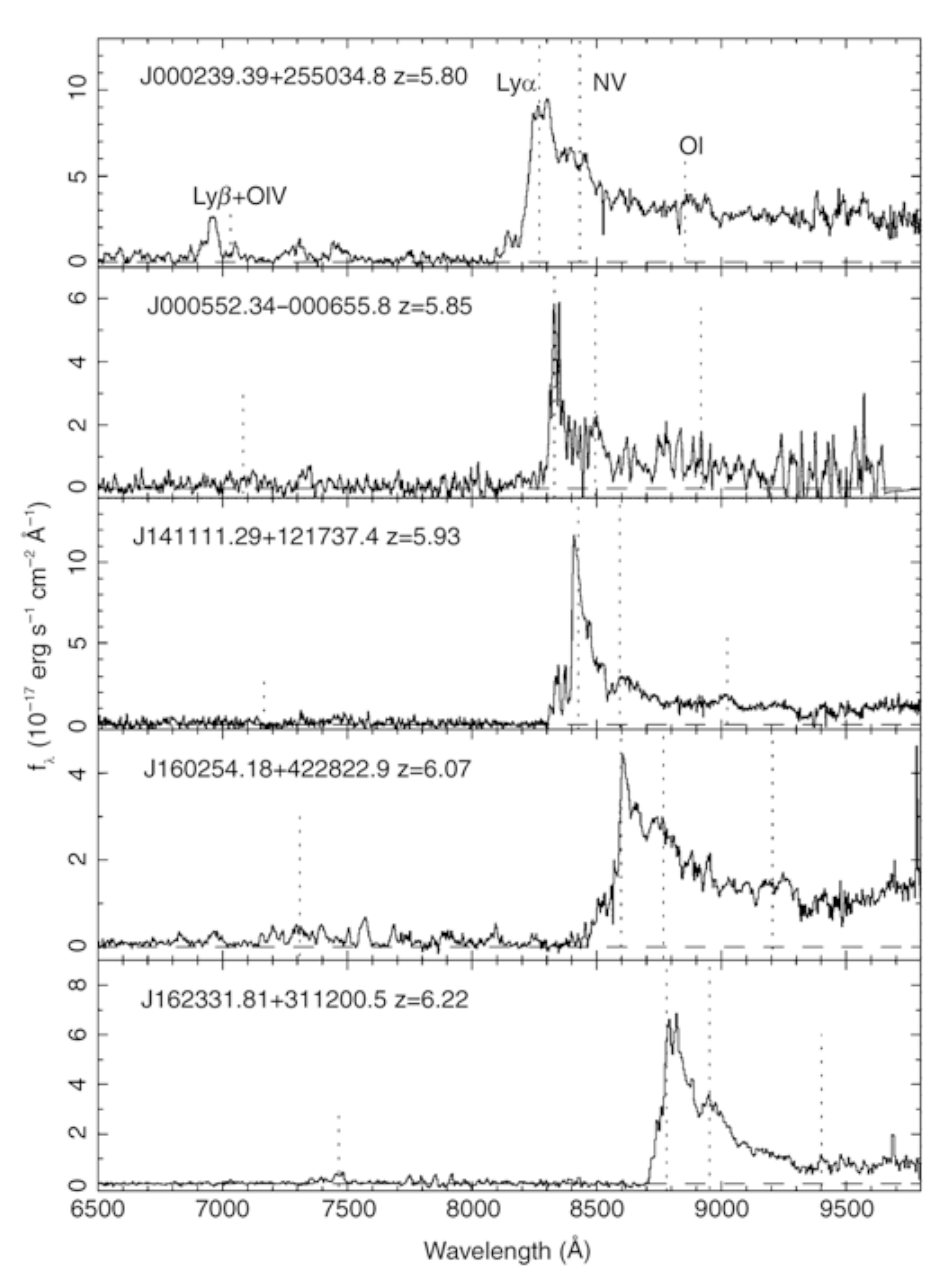
\includegraphics[width=9cm]{figures/cosmology/QSOabsorption.png}}
\end{figure}

{\noindent}which is about the average velocity of the gas particles, and $m$ denotes the average particle mass in the gas. For the gas to be bound in the gravitational field, its gravitational binding energy needs to be larger than its thermal energy, $E_\mathrm{pot}>E_\mathrm{th}$, which yields the condition $GM>c_s^2R$. Since we have assumed an only slightly overdense region, the relation $M\sim\bar{\rho}R^3$ between mass and radius of the sphere applies. From the two latter equations, the radius can be eliminated, yielding the condition

\begin{align*}
    M > M_J \equiv \frac{\pi^{5/2}}{6}\left(\frac{c_s^2}{G}\right)^{3/2}\frac{1}{\sqrt{\bar{\rho}}} ~ [{\rm M_\odot}],
\end{align*}

{\noindent}where $M_J$ is the \textbf{Jeans mass}. The Jeans mass depends on the temperature of the gas, expressed through the sound speed $c_s$, and on the mean cosmic matter density $\bar{\rho}$. The latter can easily be expressed as a function of redshift, $\bar{\rho}(z) = \bar{\rho}_0(1+z)^3$.

{\noindent}The baryon temperature $T_b$ has a more complicated dependence on redshift. For sufficiently high redshifts, the small fraction of free electrons that remains after recombination provides a thermal coupling of the baryons to the cosmic background radiation, by means of Compton scattering. This is the case for redshifts $z>z_t$, where

\begin{align*}
    z_t \approx 140\left(\frac{\Omega_bh^2}{0.022}\right)^{2/5} ~ [{\rm dimensionless}]
\end{align*}

{\noindent}hence, $T_b(z)\approx T(z)=T_0(1+z)$ for $z>z_t$. For smaller redshifts, the density of photons gets too small to maintain this coupling, and baryons start to adiabatically cool down by the expansion, so that for $z\lesssim zt$ we obtain approximately $T_b\propto\rho_b^{2/3}\propto(1+z)^2$.

{\noindent}From these temperature dependencies, the Jeans mass then be calculated as a function of redshift. For $z_t\gtrsim z\gtrsim 1000$, $M_J$ is independent of $z$ because $c_s
\propto T^{1/2}\propto(1+z)^{1/2}$ and $\bar{\rho}\propto(1+z)^3$ and its value is

\begin{align*}
    M_J = 1.35\times10^5 \left(\frac{\Omega_mh^2}{0.15}\right)^{-1/2} ~ [{\rm M_\odot}],
\end{align*}

{\noindent}whereas for $z\gtrsim z_t$ we obtain, with $T_b\simeq1.7\times10^{-2}(1+z)^2\,{\rm K}$,

\begin{align*}
    M_J = 5.7\times10^3 \left(\frac{\Omega_mh^2}{0.15}\right)^{-1/2} \left(\frac{\Omega_bh^2}{0.022}\right)^{-3/5}\left(\frac{1+z}{10}\right)^{3/2} ~ [{\rm M_\odot}].
\end{align*}

{\noindent}Hence, gas can not fall into halos with mass lower than these values.

\begin{figure}[t]
    \floatbox[{\capbeside\thisfloatsetup{capbesideposition={right,top},capbesidewidth=4cm}}]{figure}[\FBwidth]
    {\caption{\footnotesize{The cooling function for gas with primordial composition (blue solid curve), 1/3 of the Solar metallicity (green dashed curve) and Solar metallicity (red dotted curve). On the top axis, the temperature is converted into a circular velocity. To obtain such a cooling function, one needs to assume an equilibrium state of the gas. Here it is assumed that the gas is in thermodynamical equilibrium, where the fraction of ionization states of any atom depends just on $T$ . The total cooling function shown here is a superposition of different gas cooling processes, including atomic processes and bremsstrahlung, the latter of which dominating at high $T$ where the gas is fully ionized. Source: C.M. Baugh 2006, A primer on hierarchical galaxy formation: the semi-analytical approach, arXiv:astro-ph/0610031, Fig.9. Figure taken from Ryden (2006).}}
    \label{fig:coolingfunction}}
    {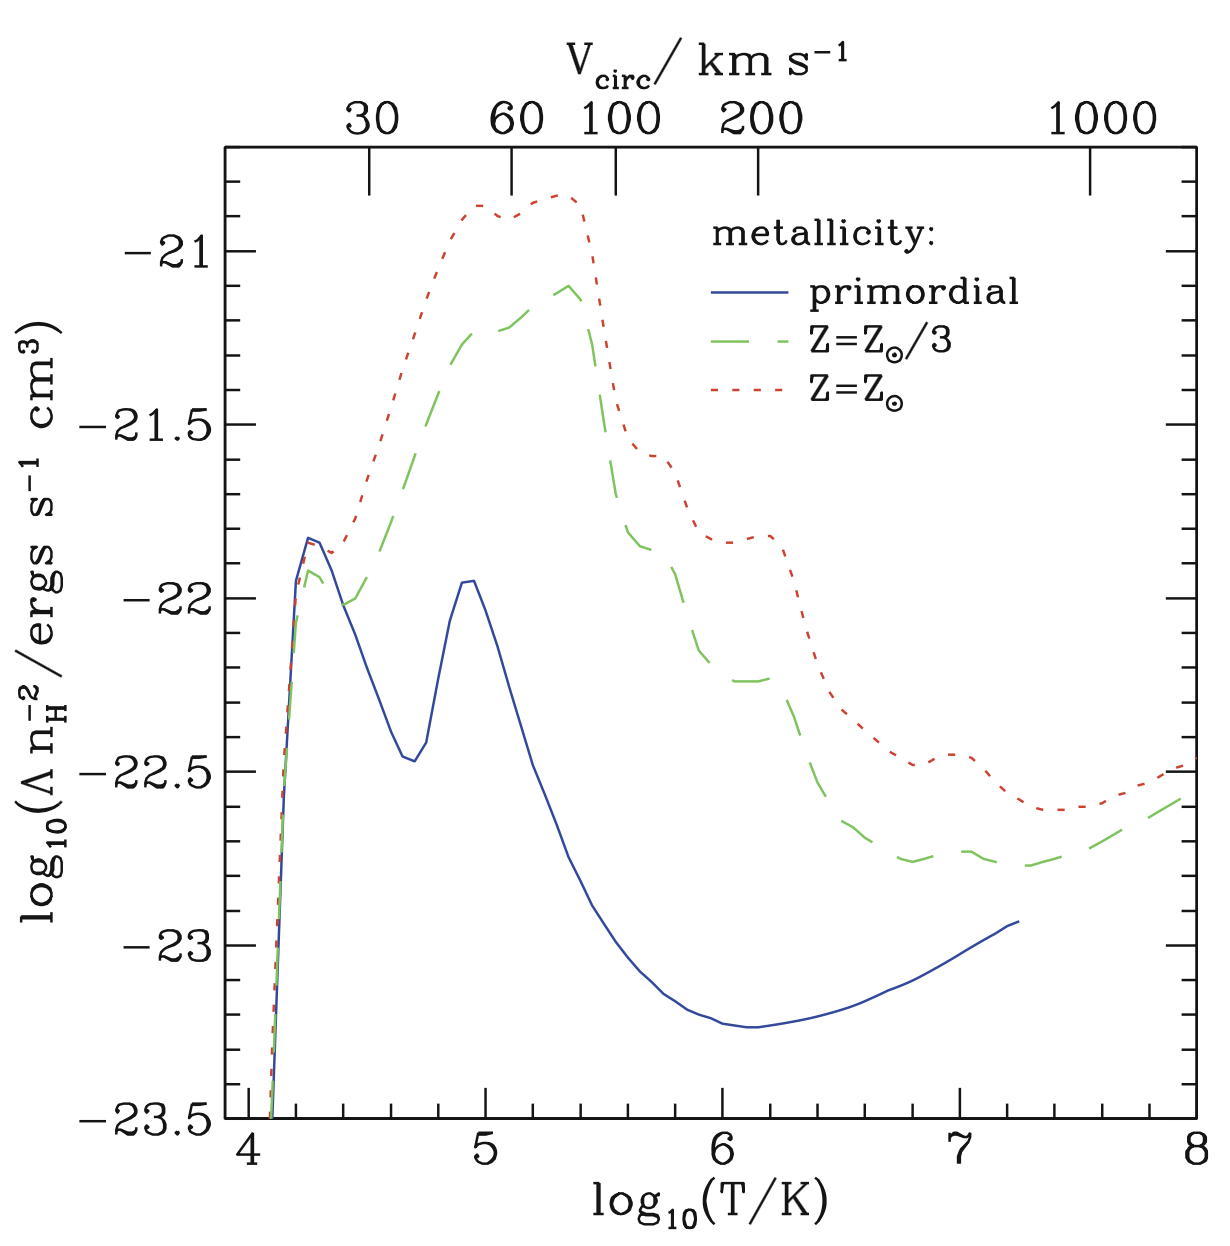
\includegraphics[width=11cm]{figures/cosmology/CoolingFunction.png}}
\end{figure}

{\noindent}The Jeans criterion is a necessary condition for the formation of proto-galaxies (i.e., dark matter halos which contain baryons). In order to form stars, the gas in the halos needs to be able to cool further. Here, we are dealing with the particular situation of the first galaxies, whose gas is metal-free, so metal lines cannot contribute to the cooling. The cooling function of primordial gas is much smaller than that of enriched material; in particular, the absence of metals means that even slow cooling though excitation of fine-structure lines cannot occur, as there are no atoms with such transitions present. Thus, cooling by the primordial gas is efficient only above $T\gtrsim2\times10^4\,{\rm K}$. However, the halos formed at high redshift have low mass. The abundance of dark matter halos depends on the parameter $\nu$ which is the ratio between the density threshold required for collapse and the dispersion of fluctuations on a given mass scale. At high redshift, the growth factor $D_+(a)$ is small, and thus to have a noticeable abundance of halos of mass $M$, the dispersion $\sigma(M)$ must be correspondingly large. At redshift $z\sim10$, the parameter $\nu$ is about unity for halos of mass $\sim10^3\,{\rm M_\odot}$. Hence, at that time, substantially more massive halos than that were (exponentially) rare (i.e., only low-mass halos were around) and their virial temperature

\begin{align*}
    T_\mathrm{vir} \approx 2\times10^2 \left(\frac{M}{10^5h^{-1}\,{\rm M_\odot}}\right)^{2/3} \left(\frac{1+z}{10}\right) ~ [{\rm K}]
\end{align*}

{\noindent}is considerably below the energy scale where atomic hydrogen can efficiently cool. Here, we used the fact that the mean matter density of a halo inside its virial radius is   200 times the critical density at a given redshift. Therefore, atomic hydrogen is a very inefficient coolant for these first halos, insufficient to initiate the formation of stars. Furthermore, helium is of no help in this context, since its excitation temperature is even higher than that of hydrogen.

\begin{figure}[t]
    \floatbox[{\capbeside\thisfloatsetup{capbesideposition={right,top},capbesidewidth=4cm}}]{figure}[\FBwidth]
    {\caption{\footnotesize{Cooling rate as a function of the temperature for a gas consisting of atomic and molecular hydrogen (with 0.1\% abundance) and of helium. The solid curve describes the cooling by atomic gas, the dashed curve that by molecular hydrogen; thus, the latter is extremely important at temperatures below $\sim10^4\,{\rm K}$. At considerably lower temperatures the gas cannot cool, hence no star formation can take place. Source: R. Barkana \& A. Loeb 2000, In the Beginning: The First Sources of Light and the Reionization of the Universe, astro-ph/0010468, Fig. 12. Figure taken from Ryden (2006).}}
    \label{fig:coolingfunctionhydrogen}}
    {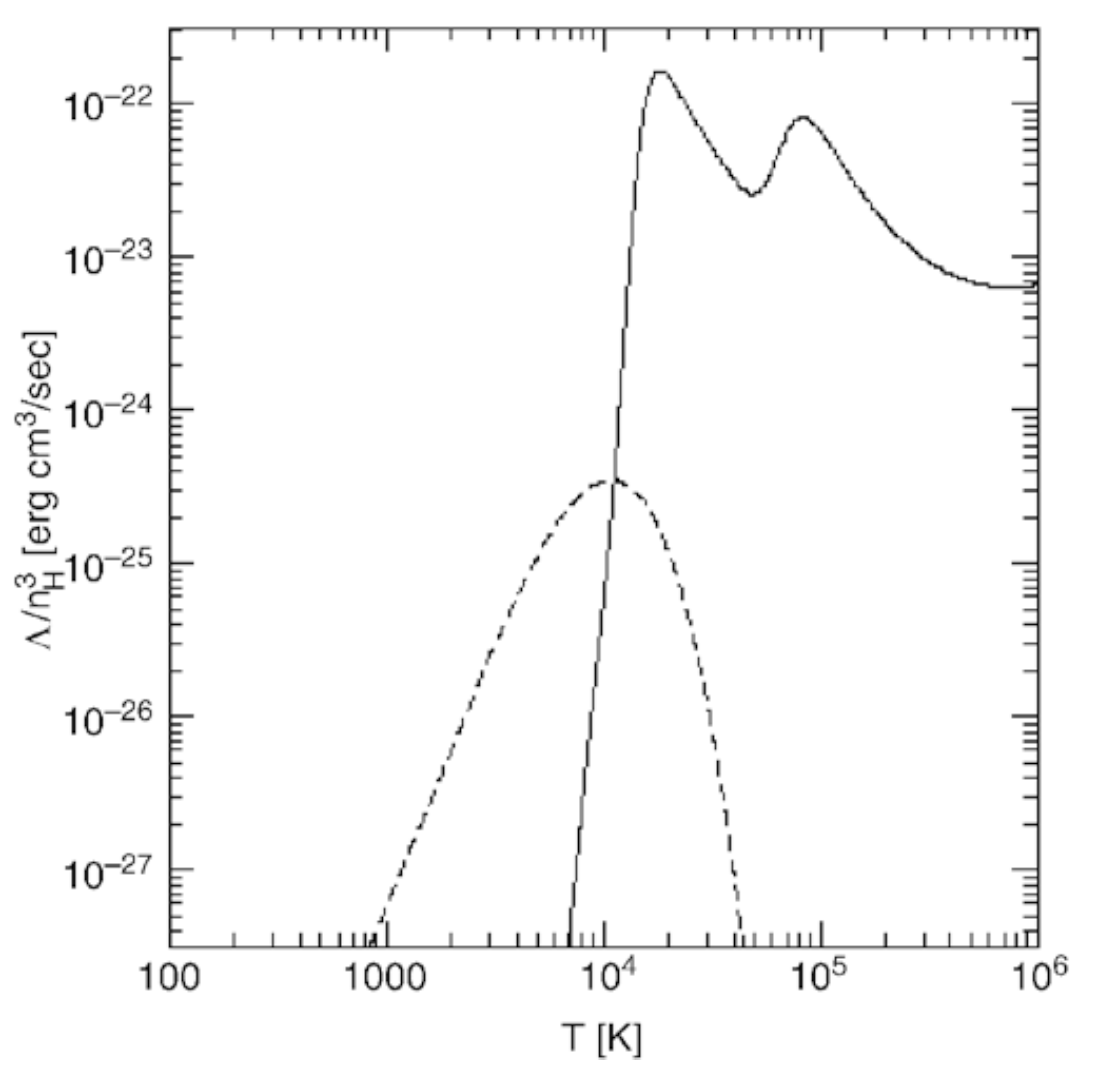
\includegraphics[width=9cm]{figures/cosmology/CoolingFunctionHydrogen.png}}
\end{figure}

{\noindent}Besides atomic hydrogen and helium, the primordial gas contains a small fraction of molecular hydrogen which represents an extremely important component in cooling processes. Whereas in enriched gas, molecular hydrogen is formed on dust particles, the primordial gas had no dust, and so H$_2$ must form in the gas phase itself, rendering its abundance very small. However, despite its very small density and transition probability, H$_2$ dominates the cooling rate of primordial gas at temperatures below $T\sim10^4\,{\rm K}$ (see Figure \ref{fig:coolingfunctionhydrogen}) where the precise value of this temperature depends on the abundance of H$_2$.

{\noindent}By means of H$_2$, the gas can cool in halos with a temperature exceeding about $T_\mathrm{vir}\gtrsim1000\,{\rm K}$, corresponding to a halo mass of $M\gtrsim5\times10^4\,{\rm M_\odot}$ at $z\sim20$. In these halos, stars may then be able to form. These stars will certainly be different from those known to us, because they do not contain any metals. Therefore, the opacity of the stellar plasma is much lower. Such stars, which at the same mass presumably have a much higher temperature and luminosity (and thus a shorter lifetime), are called population III stars. Due to their high temperature they are much more efficient sources of ionizing photons than stars with `normal' metallicity.

{\noindent}The energetic photons from these population III stars are now capable of ionizing hydrogen in their vicinity. More important still is another effect: photons with energy above $11.26eV$ can destroy H$_2$. Since the Universe is transparent for photons with energies below $13.6\,{\rm eV}$, photons with $11.26\,{\rm eV}\geq E \geq 13.6\,{\rm eV}$ can propagate very long distances and dissociate molecular hydrogen. This means that as soon as the first stars have formed in a region of the Universe, molecular hydrogen in their vicinities will be destroyed and further gas cooling and star formation will then be prevented. At this point, the Universe contains a low number density of isolated bubbles of ionized hydrogen, centered on those halos in which population III stars were able to form early, but this constitutes only a tiny fraction of the volume; most of the baryons remain neutral.

{\noindent}Soon after population III stars have formed, they will explode as supernovae. Through this process, the metals produced by them are ejected into the IGM, by which the initial metal enrichment occurs. The kinetic energy transferred by SNe to the gas within the halo can exceed its binding energy, so that the baryons of the halo can be blown away and further star formation is prevented. Whether this effect may indeed lead to gas-free halos, or whether the released energy can instead be radiated away, depends on the geometry of the star-formation regions. In any case, it can be assumed that in those halos where the first generation of stars was born, further star formation was considerably suppressed, particularly since all molecular hydrogen was destroyed.

{\noindent}We can assume that the metals produced in these first SN explosions are, at least partially, ejected from the halos into the IGM, thus enriching the latter. The existence of metal formation in the very early Universe is concluded from the fact that even sources at very high redshift (like QSOs at $z\sim6$) have a metallicity of about one tenth the Solar value. Furthermore, the Ly$\alpha$ forest also contains gas with non-vanishing metallicity. Since the Ly$\alpha$ forest is produced by the IGM, this therefore must have been enriched.

{\noindent}For gas to cool in halos without molecular hydrogen, their virial temperature needs to exceed about $10^4\,{\rm K}$ (see Figure \ref{fig:coolingfunctionhydrogen}). Halos of this virial temperature form with appreciable abundance at redshifts of $z\sim10$, corresponding to a halo mass of $\sim10^7\,{\rm M_\odot}$, as can be estimated from the Press-Schechter model. In these halos, efficient star formation can then take place and the first proto-galaxies form. These then ionize the surrounding IGM in the form of HII-regions, as sketched in Figure \ref{fig:reionization}. The corresponding HII-regions expand because increasingly more photons are produced. If the halo density is sufficiently high, these HII-regions start to overlap and soon after fill the whole volume. Once this occurs, the IGM is ionized, and reionization is completed.

\begin{figure}[t]
    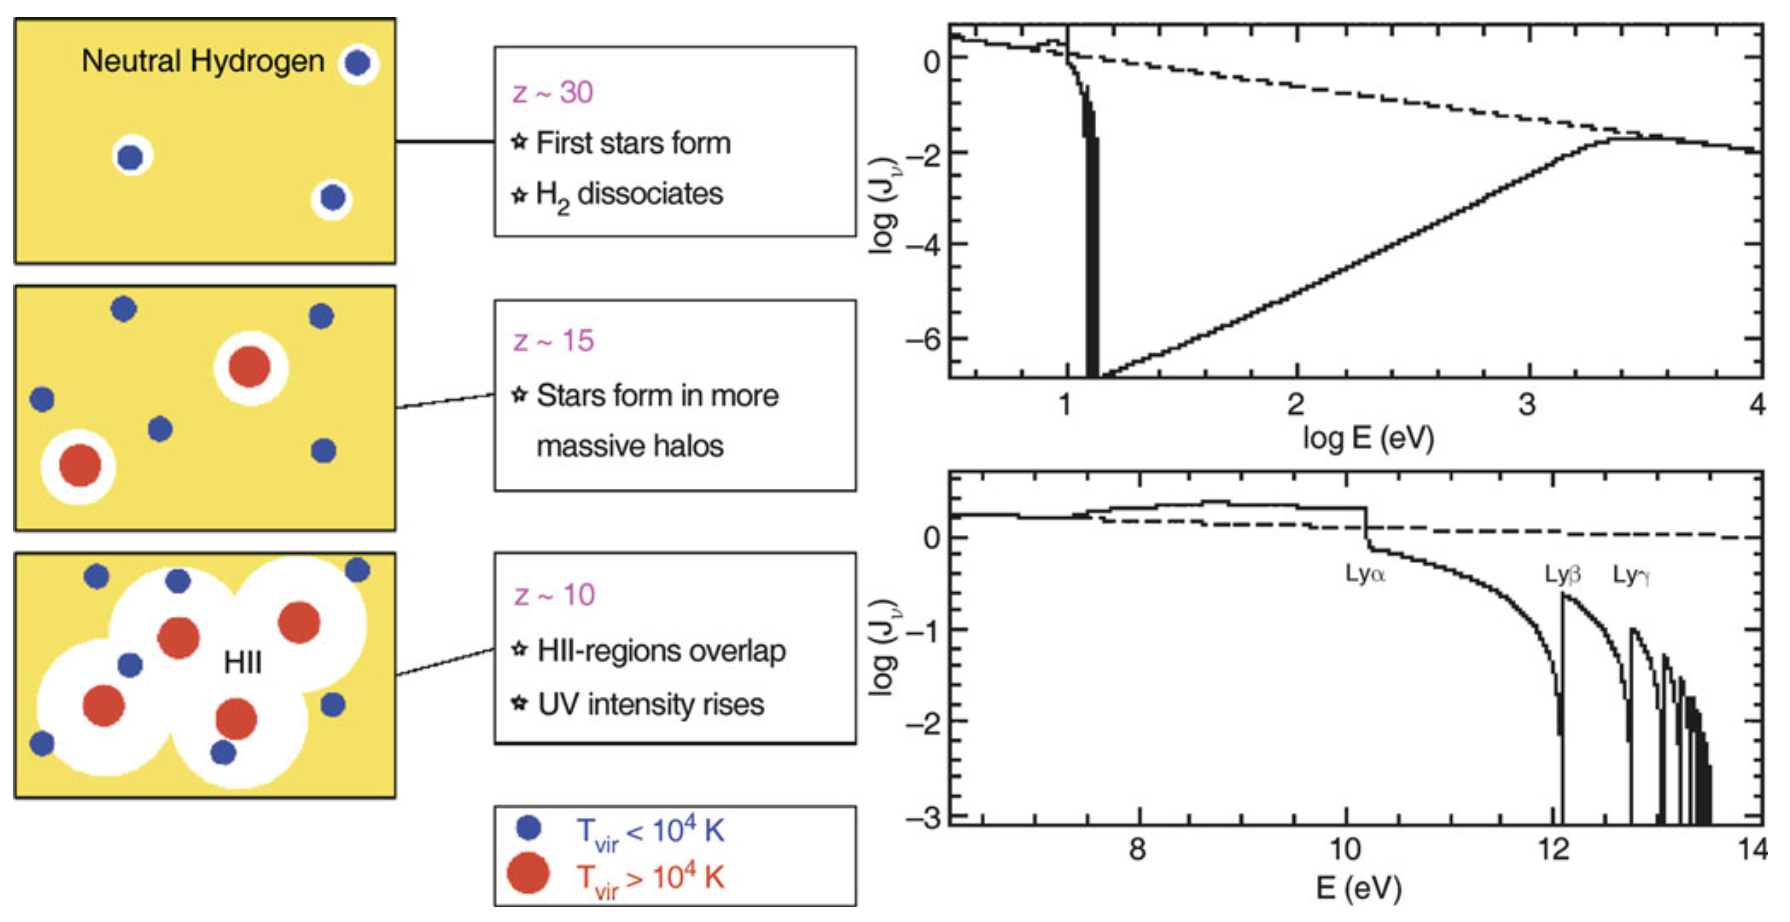
\includegraphics[width=16cm]{figures/cosmology/reionization.png}
    \centering
    \caption{\footnotesize{\textit{On the left}, a sketch of the geometry of reionization is shown: initially, relatively low-mass halos collapse, a first generation of stars ionizes and heats the gas in and around these halos. By heating, the temperature increases so strongly (to about $T\sim10^4\,{\rm K}$) that gas can escape from the potential wells; these halos may never again form stars efficiently. Only when more massive halos have collapsed will continuous star formation set in. Ionizing photons from this first generation of hot stars produce HII-regions around their halos, which is the onset of reionization. The regions in which hydrogen is ionized will grow until they start to overlap; at that time, the flux of ionizing photons will strongly increase. \textit{On the right}, the average spectrum of photons at the beginning of the reionization epoch is shown; here, it has been assumed that the flux from the radiation source follows a power law (dashed curve). Photons with an energy higher than that of the Ly$\alpha$ transition are strongly suppressed because they are efficiently absorbed. The spectrum near the Lyman limit shows features which are produced by the combination of breaks corresponding to the various Lyman lines, and the redshifting of the photons. Source: R. Barkana \& A. Loeb 2000, In the Beginning: The First Sources of Light and the Reionization of the Universe, astro-ph/0010468, Figs. 4, 11. Image taken from Ryden (2006).}}
    \label{fig:reionization}
\end{figure}

{\noindent}We therefore conclude that reionization is a two-stage process. In a first phase, population III stars form through cooling of gas by molecular hydrogen, which is then destroyed by these very stars. Only in a later epoch and in more massive halos cooling is provided by atomic hydrogen, leading to reionization.

{\noindent}The increase of temperature causes an increase of the Jeans mass, due to its dependence on the sound speed. Once the IGM is heated to $\sim10^4\,{\rm K}$ by intergalactic UV radiation, the gas pressure prevents gas inflow into low-mass halos, corresponding to circular velocities $\lesssim30\,{\rm km\,s^{-1}}$. For this reason, one expects that halos of lower mass have a lower baryon fraction than that of the cosmic mixture, $f_b=\Omega_b/\Omega_m$. The actual value of the baryon fraction depends on the details of the merger history of a halo. Quantitative studies yield an average baryon mass of

\begin{align*}
    \bar{M}_b = \frac{f_b M}{[1+(2^{\alpha/3}-1)(M_C/M)^\alpha]^{3/\alpha}} ~ [{\rm kg}],
\end{align*}

{\noindent}where $M_C\sim10^9\,{\rm M_\odot}$ is a characteristic mass, defined such that for a halo with mass $M_C$, $\bar{M}_b/M=f_b/2$. For halos of mass smaller than $M_C$, the baryon fraction is suppressed, decreasing as $(M/M_C)^3$ for small masses, whereas for halo masses $\gg M_C$, the baryon fraction corresponds to the cosmic average. The index $\alpha\sim2$ determines the sharpness of the transition between these two cases. The characteristic mass $M_C$ depends on redshift, being much smaller at high $z$ due to the stronger ionizing background.

{\noindent}The ionizing flux has two additional effects on the gas that resides in halos: it provides a source of heating due to photoionization and it leads to a higher degree of ionization in the gas, reducing the number density of atoms which can be excited by collisions and cool through de-excitation. Both effects act in the same direction, by impeding an efficient cooling of the gas and hence the formation of stars. For halos of larger mass, intergalactic radiation is of fairly little importance because the corresponding heating rate is substantially smaller than that occurring by the dissipation of the gas which is needed to concentrate the baryons towards the halo center. For low-mass halos, however, this effect is important. Together, these two effects reduce the cooling rate of the gas, which is a dominant effect for low-mass halos. Thus, the gas in low-mass halos cannot cool efficiently, suppressing star formation -- unless star formation occurred before the reionization was completed. We hence found one of the elements for the second part of the answer to the question about the different mass-to-light ratios in halos: star formation in low mass halos is strongly suppressed due to the ionizing background radiation. This also provides an explanation of the `missing satellite problem'.

{\noindent}To singly ionize helium, photons of energy $\geq24.6\,{\rm eV}$ are required, and the ionization energy of He II is four times that of hydrogen. In addition, the recombination rate of fully ionized helium is about five times higher than that of hydrogen. Therefore, the reionization of helium is expected to be completed at a later epoch when the density of photons with $\lambda<304$\,\AA was high enough. Since even massive stars do not generate photons exceeding this energy in large quantities, the photons leading to helium reionization presumably are emitted by quasars; therefore, the ionization of helium has to wait for the `quasar epoch' of the Universe, at $z\lesssim4$. From the statistical analysis of the Ly$\alpha$ forest and from the analysis of helium absorption lines and the helium Gunn-Peterson effect in high-redshift QSOs, a reionization redshift of $z\sim3$ for helium is obtained.

{\noindent}One of the challenges of current observational cosmology is to link the history of reionization, as outlined above, to the observation of the highest redshift sources (i.e., to see whether we can observe the sources which are responsible for cosmic reionization). Are the galaxy populations that we can find at very high redshifts sufficient to understand the reionization process? Here we shall mention some of the major obstacles for a direct observation probe of these ionizing sources.

\begin{figure}[t]
    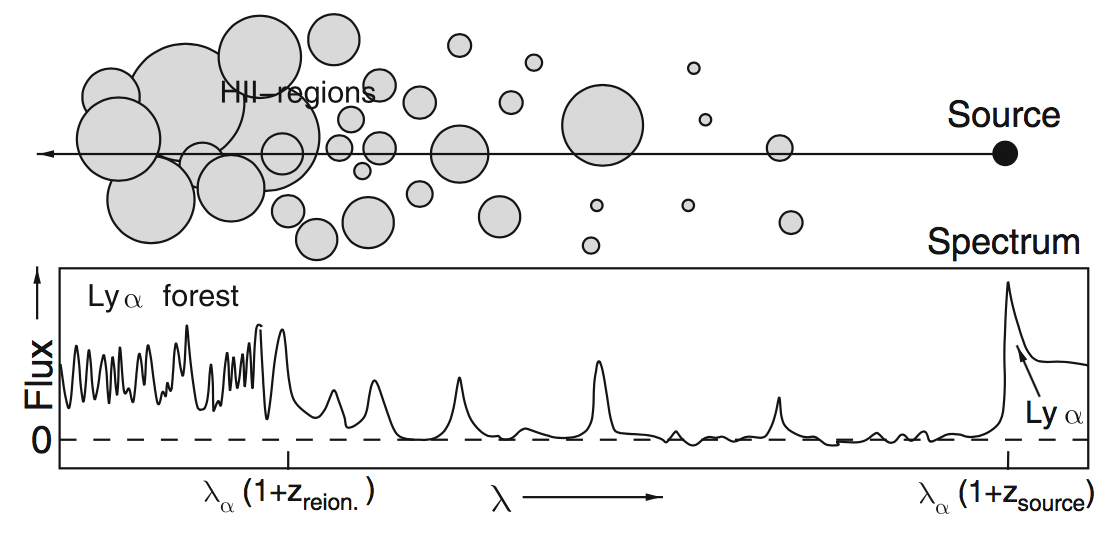
\includegraphics[width=14cm]{figures/cosmology/LyaForest.png}
    \centering
    \caption{\footnotesize{Sketch of a potential observation of reionization: light from a very distant QSO propagates through a partially ionized Universe; at locations where it passes through HII-regions, radiation will get through -- flux will be visible at the corresponding wavelengths. When the HII-regions start to overlap, the normal Ly$\alpha$ forest will be produced. Adapted from: R. Barkana \& A. Loeb 2000, In the Beginning: The First Sources of Light and the Reionization of the Universe, astro-ph/0010468. Figure taken from Ryden (2006).}}
    \label{fig:lyaforest}
\end{figure}

{\noindent}If reionization was caused by the energetic photons emitted during star formation, the remnants of this first generation of stars must be present in the post-reionization Universe, and thus be observable. Galaxies at redshift $z>6$ are observed, either as Lyman-break galaxies (LBGs), Lyman-alpha emitters (LAEs) or as sub-millimeter galaxies (SMGs). Their stellar masses can be estimated from their observed light. However, most of the LBGs are observed only in the near-IR, which means that we see their restframe UV-emission. Converting the UV-light into a stellar mass is highly uncertain, since it depends strongly on the instantaneous star-formation rate. For LAEs, it is even more challenging to determine a stellar mass, since they are typically fainter in their broad-band (i.e., continuum) emission, which renders the determination of the stellar mass even more challenging.

{\noindent}Nevertheless, galaxies at very high redshift were found which appear to have high stellar masses, including a LAE at $z=6.6$ with an estimated stellar mass $M_*\gtrsim10^{11}\,{\rm M_\odot}$. The high-redshift QSOs require a SMBH with $M\gtrsim10^9\,{\rm M_\odot}$ to power their energy output, and these must be hosted in galaxies with very large stellar masses. Therefore, massive galaxies have formed very early on, delivering ionizing photons.

{\noindent}However, these highest mass objects are very rare and, by themselves, by far not able to explain reionization. This fact can be clearly seen by considering the spectral shape of the Ly$\alpha$ emission line of high-redshift QSOs. Figure \ref{fig:lyaforest} describes qualitatively the result of observing the emission towards bright background QSOs to study (re)ionization. Figure \ref{fig:qsoreionization} shows the spectrum of three very high redshift QSOs near to the Lyman$\alpha$Ìš emission line. Whereas all three QSO show essentially no flux blueward of Lyman$\alpha$, once the wavelength difference exceeds $\sim20$ {\AA} in the restframe, there is some transmitted flux very close to the Ly$\alpha$ transition. This near-zone transmission is understood as a region around the QSO where the intergalactic gas is fully ionized by the QSO, so it becomes transparent. The figure shows a clear trend that the size of this near zone decreases for higher redshifts, as would be expected due to the higher gas density and probably larger mean neutral fraction in the Universe. Thus, these very luminous objects are able to reionize the IGM in their immediate surroundings, but their effect is constrained to a rather limited volume. Most of the ionizing photons must come from the far more numerous lower-mass galaxies (i.e., far less luminous sources).

\begin{figure}[t]
    \floatbox[{\capbeside\thisfloatsetup{capbesideposition={right,top},capbesidewidth=4cm}}]{figure}[\FBwidth]
    {\caption{\footnotesize{The spectra of three high-redshift QSOs (SDSSJ1148+5251 at $z=6.42$, SDSS J1030+0524 at $z=6.31$, and the $z=7.085$ QSO ULAS J1120+0641) at the Lyman$\alpha$ emission line. For this figure, the wavelength difference to the Lyman$\alpha$ transition is expressed in proper distance away from the QSOs. The spectra are normalized, dividing them by the extrapolation of the continuum on the red side of the emission line, yielding the transmission. Source: D.J. Mortlock et al. 2011, A luminous quasar at a redshift of $z=7.085$, Nature 474, 616, Fig. 3. Figure taken from Ryden (2006).}}
    \label{fig:qsoreionization}}
    {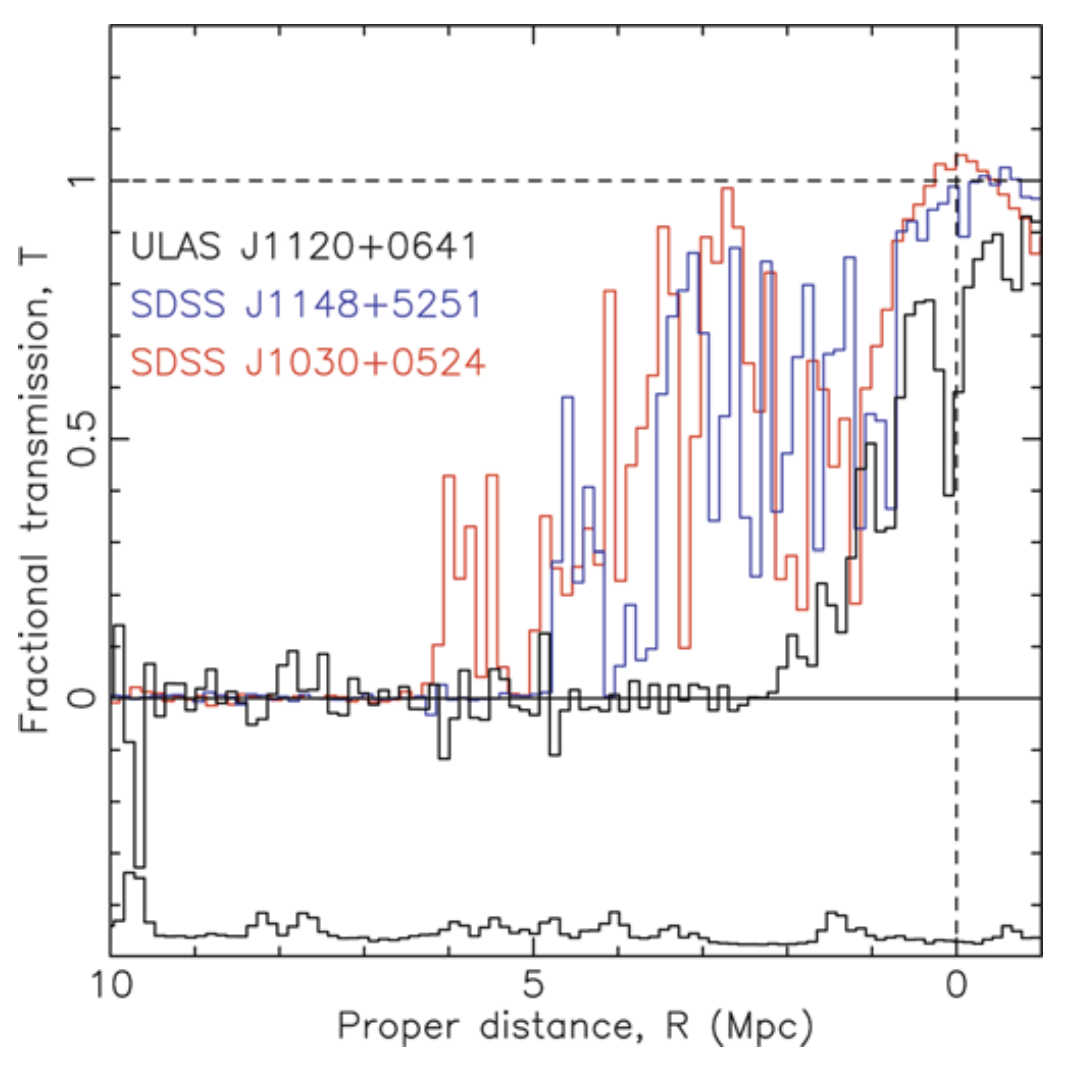
\includegraphics[width=9cm]{figures/cosmology/QSOreionization.png}}
\end{figure}

{\noindent}Gunn \& Peterson (1965) first proposed using Ly$\alpha$ resonance absorption in the spectrum of distant quasars as a direct probe to the neutral hydrogen density in the IGM at high redshift. For objects beyond reionization, neutral hydrogen in the IGM creates complete GP absorption troughs in the quasar spectrum blueward of Ly$\alpha$ emission. Observations of the GP effect directly constrain the evolution of neutral hydrogen fraction and the ionization state of the IGM.

{\noindent}The Gunn-Peterson optical depth to Ly$\alpha$ photons is

\begin{align*}
    \tau_\mathrm{GP} = \frac{\pi e^2}{m_ec^2}f_\alpha\lambda_\alpha H^{-1}(z)n_\mathrm{HI} ~ [{\rm dimensionless}],
\end{align*}

{\noindent}where $f_\alpha$ is the oscillator strength of the Ly$\alpha$ transition, $\lambda_\alpha=1216$\,\AA, $H(z)$ is the
Hubble constant at redshift $z$, and $n_\mathrm{HI}$ is the density of neutral hydrogen in the IGM.

{\noindent}At high redshifts,

\begin{align*}
    \tau_\mathrm{GP}(z) = 4.9\times10^5 \left(\frac{\Omega_mh^2}{0.13}\right)^{-1/2} \left(\frac{\Omega_bh^2}{0.02}\right) \left(\frac{1+z}{7}\right)^{3/2} \left(\frac{n_\mathrm{HI}}{n_\mathrm{H}}\right) ~ [{\rm dimensionless}]
\end{align*}

{\noindent}for a uniform IGM. Even a tiny neutral fraction, $X_\mathrm{HI}\sim10^{-4}$, gives rise to complete GP absorption. This test is only sensitive at the end of the reionization when the IGM is already mostly ionized, and the absorption saturates for the higher neutral fraction in the earlier stage.

{\noindent}At $z<5$, the IGM absorption is resolved into individual Ly$\alpha$ forest lines; their number density increases strongly with redshift: $N_\alpha(z)\propto(1+z)$. Earlier attempts to study GP absorption concentrated on measuring the amount of flux between individual Ly$\alpha$ forest lines using high-resolution spectroscopy to place limits on the diffuse neutral IGM. However, at $z>5$, even with a moderately high resolution spectrum, Ly$\alpha$ forest lines overlap severely, making it impossible to find a truly ``line-free'' region.

{\noindent}A more accurate picture of the IGM evolution interprets the Ly$\alpha$ forest as a fluctuating GP effect: absorption arises from low-density gas in the IGM that is in approximate thermal equilibrium between photoionization heating by the UV background and adiabatic cooling due to the Hubble expansion, rather than as discrete Lyα$\alpha$ forest clouds. The neutral hydrogen fraction and therefore the GP optical depth
depend on the local density of the IGM. By studying the evolution of the average transmitted flux or effective optical depth, one can trace the evolution of the UV ionizing background and neutral fraction of the IGM. At high-redshift, the IGM is highly clumpy, which must be taken into account in order to estimate the IGM ionization from observations.

\begin{figure}[t]
    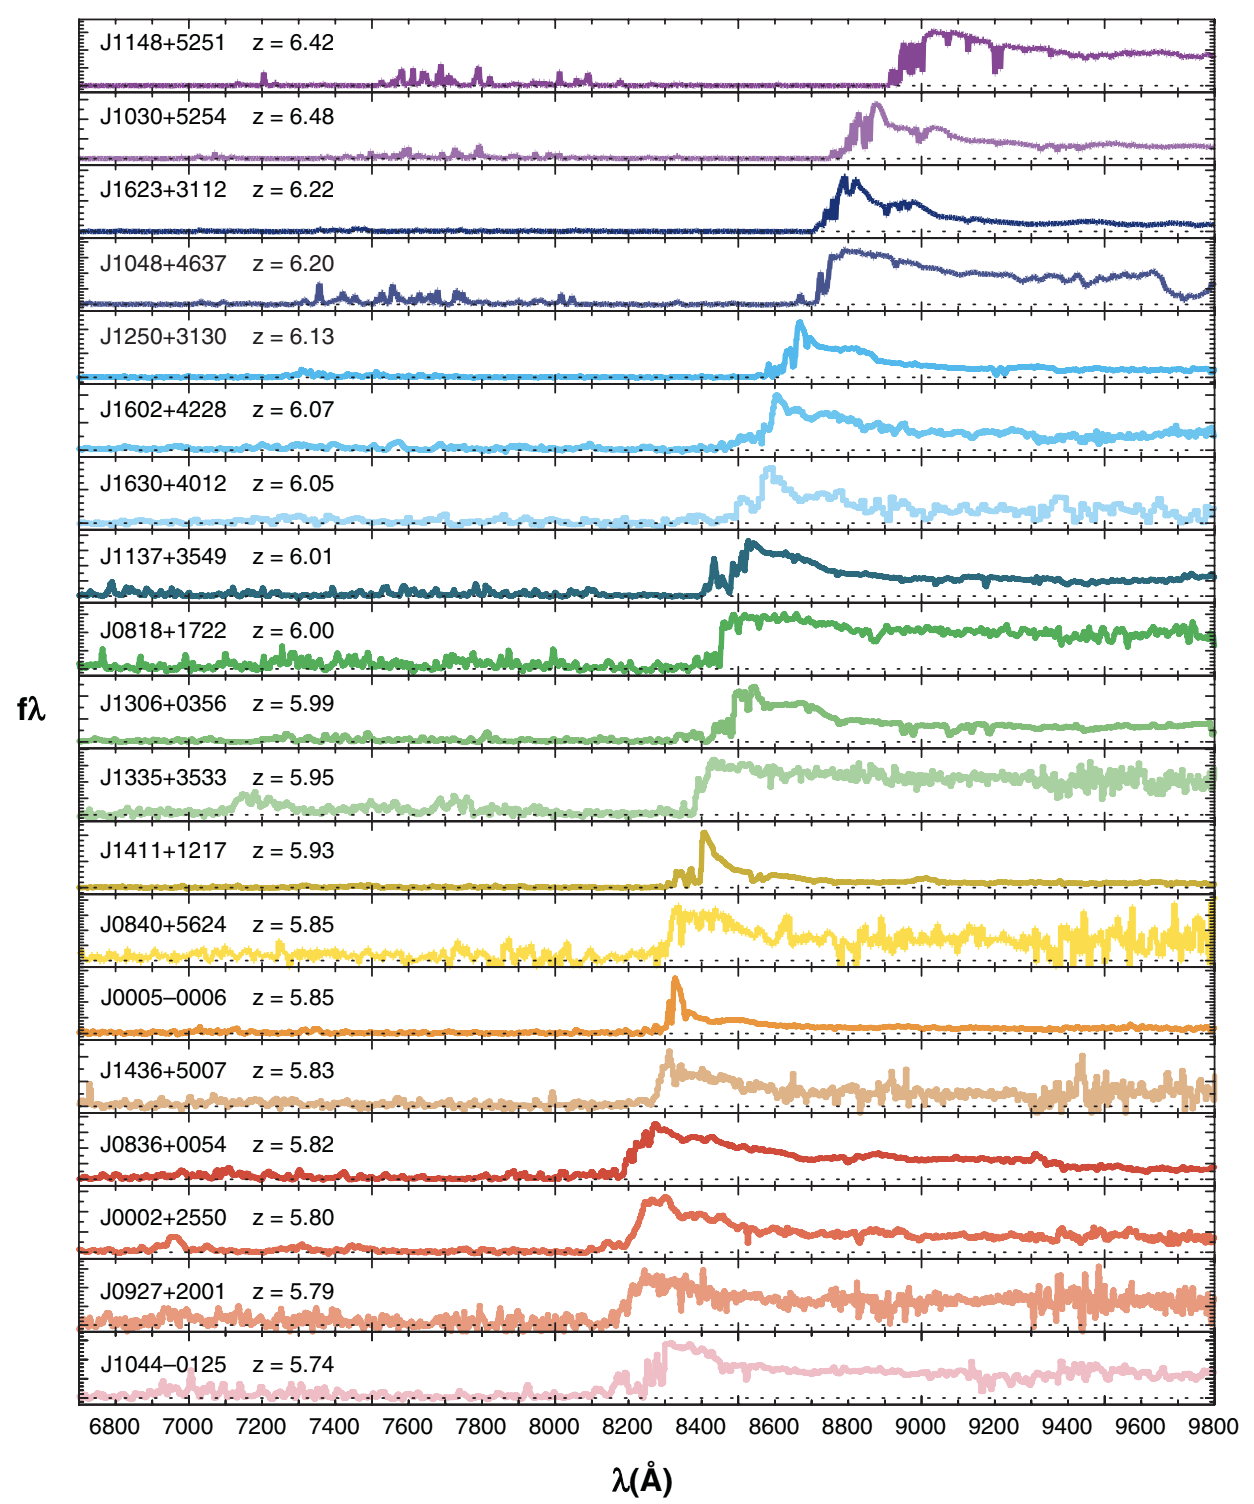
\includegraphics[width=14cm]{figures/cosmology/SDSSQSO.png}
    \centering
    \caption{\footnotesize{Moderate resolution spectra of nineteen SDSS quasars at $5.74<z<6.42$. Adapted from Fan et al. (2006b). Image taken from Ryden (2006).}}
    \label{fig:sdssqso}
\end{figure}

{\noindent}The SDSS provides large samples of luminous quasars over $0<z<6.5$. Fan et al. (2000, 2001a,b, 2003, 2004, 2006a) carried out a survey of i-dropout quasars ($z>5.7$) using the SDSS imaging data, resulting in the discovery of 19 luminous quasars in this redshift regime (Figure \ref{fig:sdssqso}). Other multicolour survey projects are also searching for quasars at similar redshifts. They provide by far the best probes of IGM evolution toward the end of the EoR.

\begin{figure}[t]
    \floatbox[{\capbeside\thisfloatsetup{capbesideposition={right,top},capbesidewidth=4cm}}]{figure}[\FBwidth]
    {\caption{\footnotesize{Redshift evolution of the mean neutral fraction of hydrogen in the IGM, as obtained from the absorption of ionizing radiation from high-redshift QSOs (Gunn-Peterson effect). Individual measurements are shown as small dots, whereas the large circles with error bars represent averages over redshift bins. The two curves show results from numerical simulations. Source: X. Fan et al. 2006, Constraining the Evolution of the Ionizing Background and the Epoch of Reionization with $z\sim6$ Quasars. II. A Sample of 19 Quasars, AJ 132, 117, p. 126, Fig. 7. Figure taken from Ryden (2006).}}
    \label{fig:hivsz}}
    {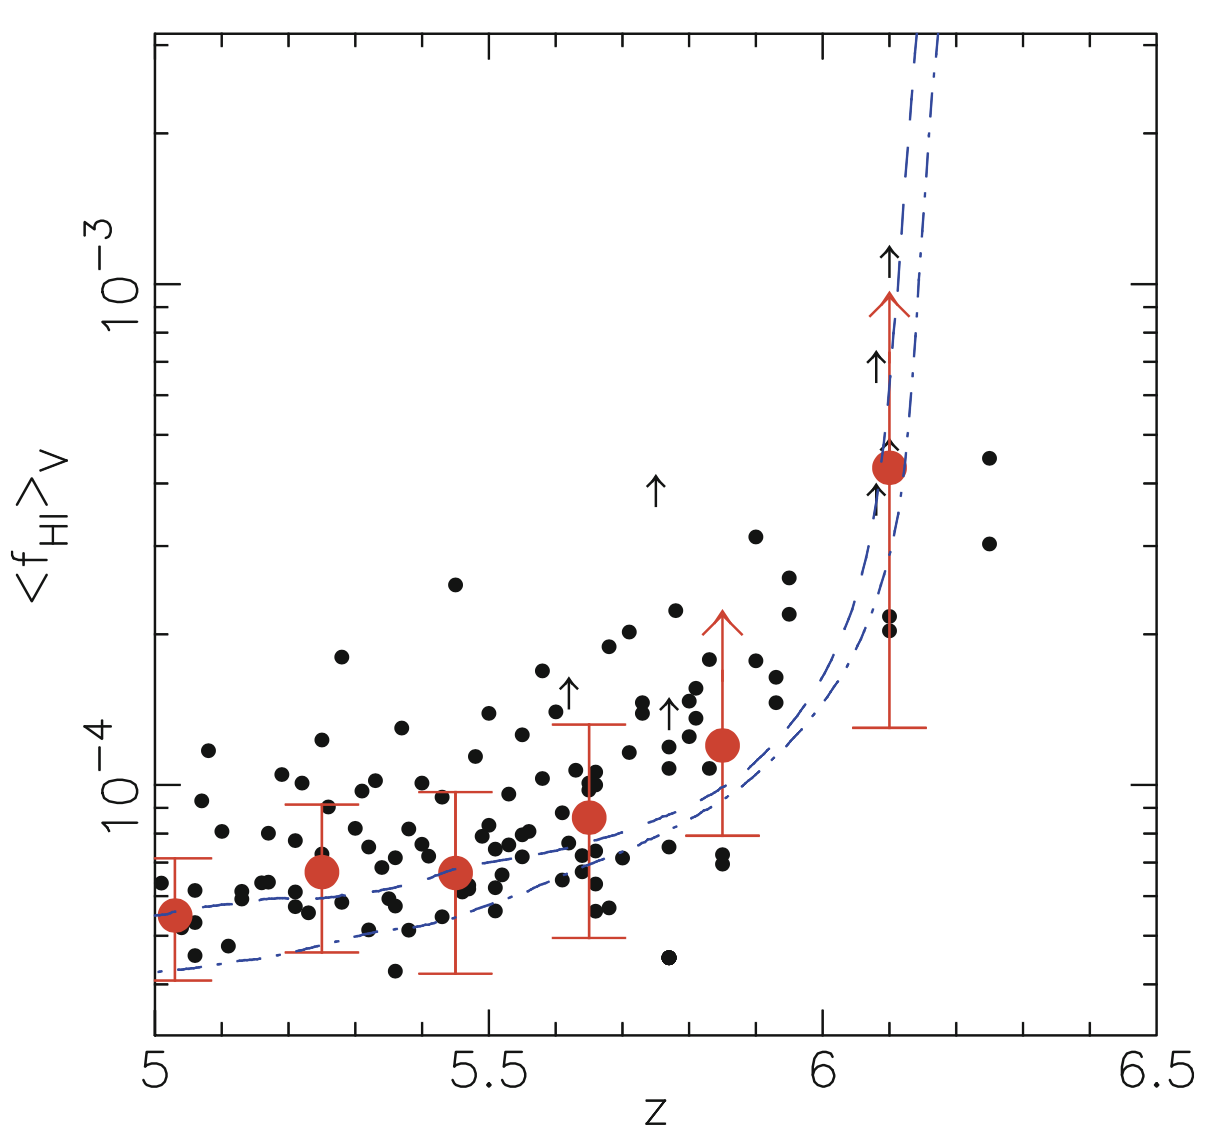
\includegraphics[width=10cm]{figures/cosmology/HIvsz.png}}
\end{figure}

{\noindent}The observed spectrum of high-redshift QSOs bluewards of the Ly$\alpha$ emission line shows that an increasing fraction of the radiation is absorbed by neutral hydrogen on the line-of-sight. We have seen that the density of the Ly$\alpha$ forest increases with redshift (see Figures \ref{fig:qsoabsorption} and \ref{fig:sdssqso}) in such a way that only a tiny fraction of ionizing photons manage to escape absorption. This observation may be seen as an indication that we approach the EoR as the QSO redshift increases beyond $z\sim6$. However, as shown in Figure \ref{fig:hivsz}, the mean neutral fraction of intergalactic hydrogen needed to cause this strong absorption of ionizing photons is still very small -- a neutral fraction of much less than 1\% is sufficient to entirely block the light of QSOs blueward of the Ly$\alpha$ emission. Hence, the strong absorption implied by QSO spectra cannot be taken as evidence for $z\sim6$ signalling the end of the EoR. Nevertheless, the trend of the data shown in Figure \ref{fig:hivsz} may suggest that beyond $z\sim6$, we may approach a phase where the neutral hydrogen fraction indeed starts to increase significantly.

{\noindent}Observing reionization directly may in principle be possible if a very high-redshift QSO could be identified whose absorption spectrum could reveal a tomographic view through the ionized `bubbles' of the IGM, as sketched in Figure \ref{fig:lyaforest}. But we point out again that the very dense Ly$\alpha$ forest seen towards QSOs at high redshift, is no unambiguous sign for approaching the redshift of reionization, because a very small fraction of neutral atoms (about 1\%) is already sufficient to produce a large optical depth for Ly$\alpha$ photons.

\subsubsection{Follow-up Questions}

\begin{itemize}
    \item Besides the first stars and galaxies, what else could have ionized the Universe?
    \item How does the recent paper by Bowman et al. relate to this?
    \item What about Helium ionization?
\end{itemize}


% --------------------------------------------------------------
%
%                           16. 
%
% --------------------------------------------------------------

\newpage
\subsection{Question 16}

The $21\,{\rm cm}$ line of hydrogen is expected to show up in absorption against the cosmic microwave background at some redshifts, and in emission at other redshifts. What physical processes lead to this behaviour?

\subsubsection{Short answer}

The key to the detectability of the $21\,{\rm cm}$ signal hinges on the spin temperature $T_s$. Only if this temperature deviates from the background temperature, will a signal be observable.

\begin{itemize}
    \item $\mathbf{200\lesssim z\lesssim 1100:}$ The residual free electron fraction left after recombination allows Compton scattering to maintain thermal coupling of the gas to the CMB, setting $T_k=T_\gamma$. The high gas density leads to effective collisional coupling so that $T_s=T_\gamma$ and we expect $\bar{T}_b=0$ and no detectable $21\,{\rm cm}$ signal.
    \item $\mathbf{40\lesssim z\lesssim 200:}$In this regime, the gas cools adiabatically so that $T_k\propto(1+z)^2$ leading to $T_k<T_\gamma$ and collisional coupling sets $T_s<T_\gamma$, leading to $\bar{T}_b<0$ and an early absorption signal. At this time, $T_b$ fluctuations are sourced by density fluctuations, potentially allowing the initial conditions to be probed.
    \item $\mathbf{z_*\lesssim z\lesssim 40:}$ As the expansion continues, decreasing the gas density, collisional coupling becomes ineffective and radiative coupling to the CMB sets $T_s=T_\gamma$, and there is no detectable $21\,{\rm cm}$ signal.
    \item $\mathbf{z_\alpha\lesssim z\lesssim z_*:}$ Once the first sources switch on at $z_*$, they emit both Ly$\alpha$ photons and X-rays. In general, the emissivity required for Ly$\alpha$ coupling is significantly less than that for heating $T_k$ above $T_\gamma$. We therefore expect a regime where the spin temperature is coupled to cold gas so that $T_s\sim T_k<T_\gamma$ and there is an absorption signal. Fluctuations are dominated by density fluctuations and variation in the Ly$\alpha$ flux. As further star formation occurs the Ly$\alpha$ coupling will eventually saturate ($x_\alpha\gg1$), so that by a redshift $z_\alpha$ the gas will everywhere be strongly coupled.
    \item $\mathbf{z_h\lesssim z\lesssim z_\alpha:}$ After Ly$\alpha$ coupling saturates, fluctuations in the Ly$\alpha$ flux no longer affect the $21\,{\rm cm}$ signal. By this point, heating becomes significant and gas temperature fluctuations source $T_b$ fluctuations. While $T_k$ remains below $T_\gamma$ we see a $21\,{\rm cm}$ signal in absorption, but as $T_k$ approaches $T_\gamma$ hotter regions may begin to be seen in emission. Eventually by a redshift $z_h$ the gas will be heated everywhere so that $\bar{T}_k=T_\gamma$.
    \item $\mathbf{z_T\lesssim z\lesssim z_h:}$ After the heating transition, $T_k>T_\gamma$ and we expect to see a $21\,{\rm cm}$ signal in emission. The $21\,{\rm cm}$ brightness temperature is not yet saturated, which occurs at $z_T$, when $T_s\sim T_k\gg T_\gamma$. By this time, the ionization fraction has likely risen above the percent level. Brightness temperature fluctuations are sourced by a mixture of fluctuations in ionization, density and gas temperature.
    \item $\mathbf{z_r\lesssim z\lesssim z_T:}$ Continued heating drives $T_k\gg T_\gamma$ at $z_T$ and temperature fluctuations become unimportant. $T_s\sim T_k\gg T_\gamma$ and the dependence on $T_s$ may be neglected which greatly simplifies analysis of the $21\,{\rm cm}$ power spectrum. By this point, the filling fraction of HII regions probably becomes significant and ionization fluctuations begin to dominate the $21\,{\rm cm}$ signal.
    \item $\mathbf{z\lesssim z_r:}$ After reionization, any remaining $21\,{\rm cm}$ signal originates primarily from collapsed islands of neutral hydrogen (damped Ly$\alpha$ systems).
\end{itemize}

{\noindent}These events are summarized in Figure \ref{fig:21cmannotated}.

\begin{figure}[t]
    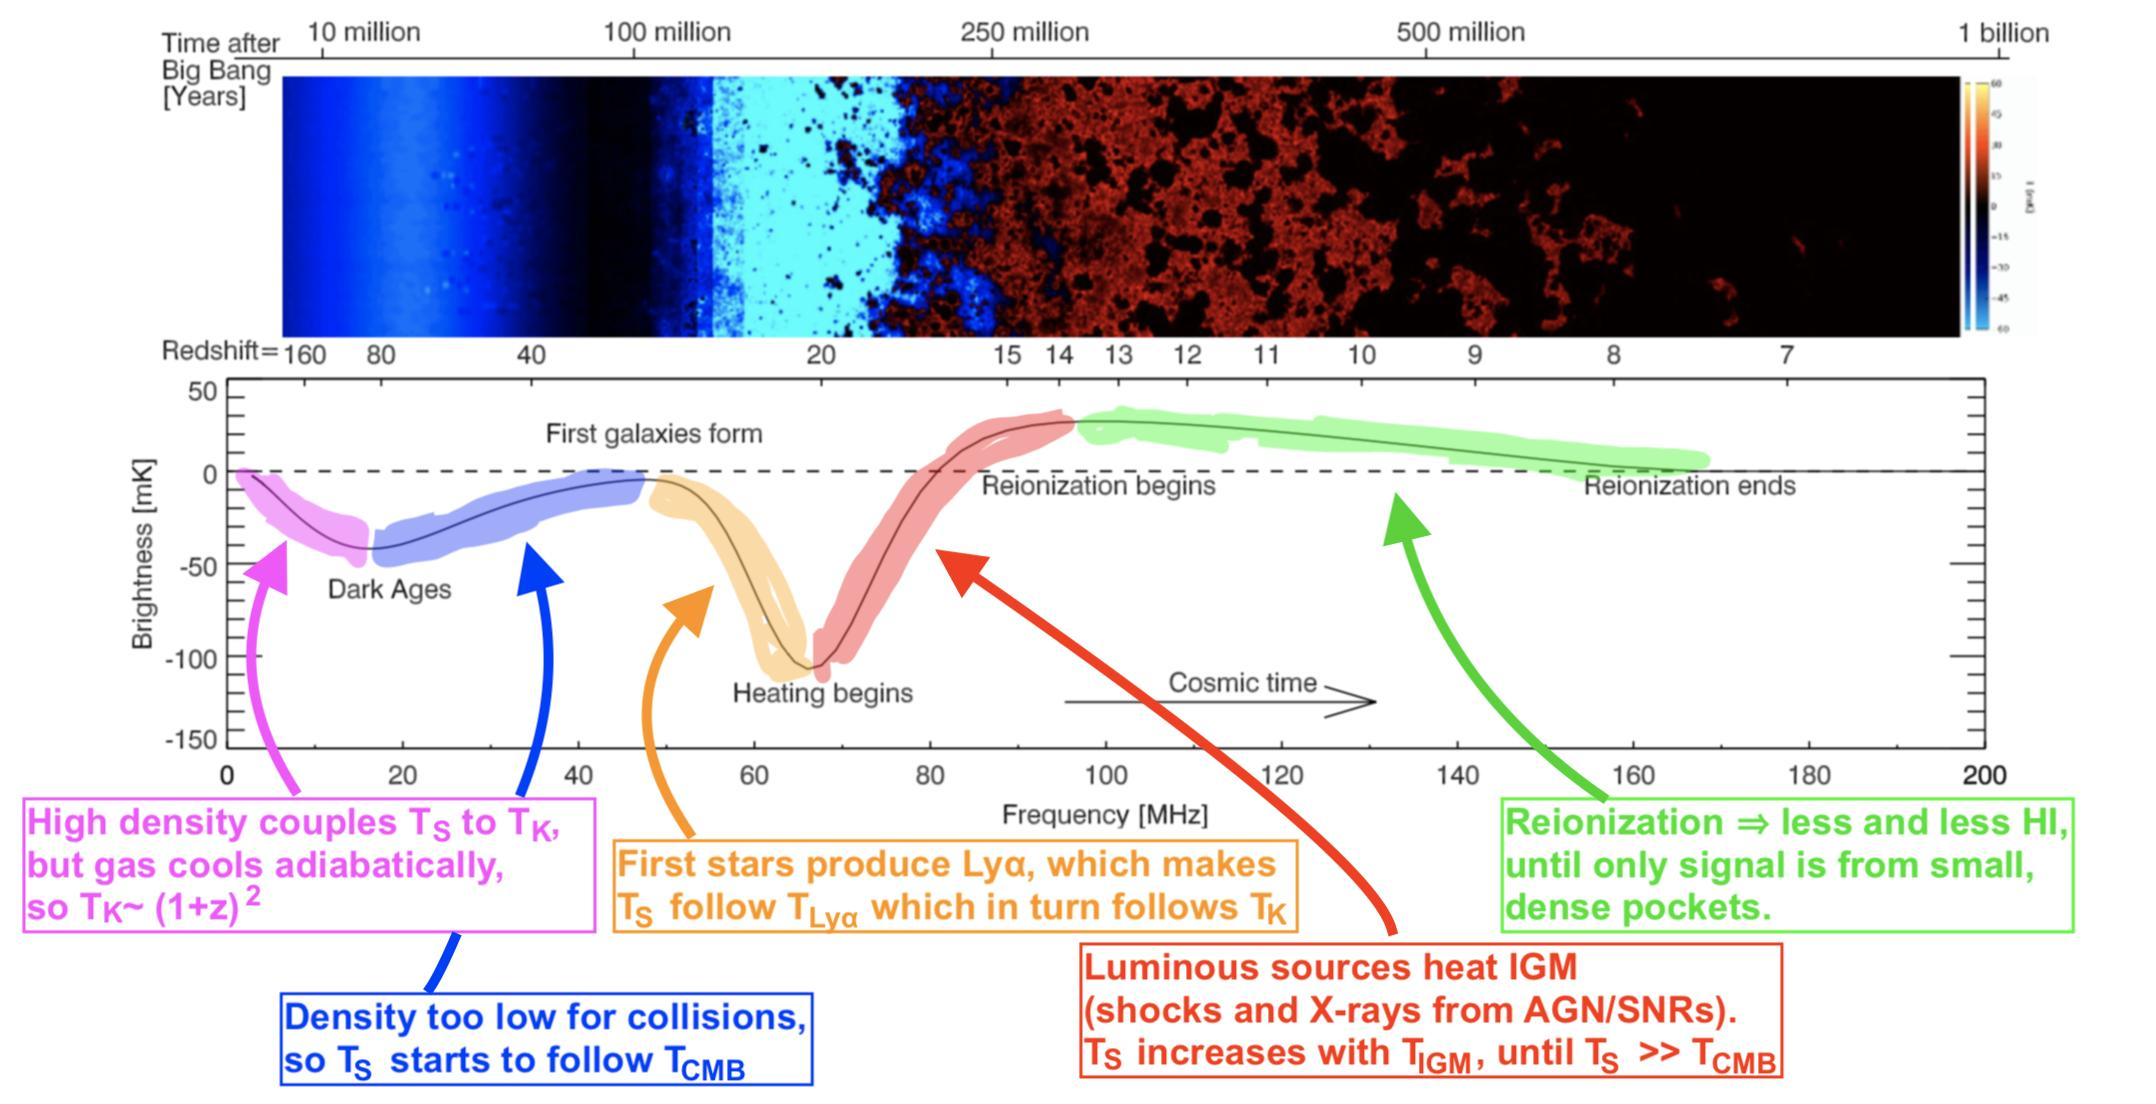
\includegraphics[width=16cm]{figures/cosmology/21cm_annotated.jpg}
    \centering
    \caption{\footnotesize{The 21-centimeter cosmic hydrogen signal. (a) Time evolution of fluctuations in the $21\,{\rm cm}$ brightness from just before the first stars formed through to the end of the EoR. This evolution is pieced together from redshift slices through a simulated cosmic volume. Colouration indicates the strength of the $21\,{\rm cm}$ brightness as it evolves through two absorption phases (purple and blue), separated by a period (black) where the excitation temperature of the $21\,{\rm cm}$ hydrogen transition decouples from the temperature of the hydrogen gas, before it transitions to emission (red) and finally disappears (black) owing to the ionization of the hydrogen gas. (b) Expected evolution of the sky-averaged $21\,{\rm cm}$ brightness from the ``dark ages'' at redshift $200$ to the end of reionization, sometime before redshift $6$ (solid curve indicates the signal; dashed curve indicates $T_b=0$). The frequency structure within this redshift range is driven by several physical processes, including the formation of the first galaxies and the heating and ionization of the hydrogen gas. There is considerable uncertainty in the exact form of this signal, arising from the unknown properties of the first galaxies. Figure taken from Ryden (2006) with annotations by Matt Young.}}
    \label{fig:21cmannotated}
\end{figure}

\subsubsection{Additional context}

{\noindent}As the most common atomic species present in the Universe, hydrogen is a useful tracer of local properties of the gas. The simplicity of its structure (a proton and electron) belies the richness of the associated physics. The $21\,{\rm cm}$ line of hydrogen arises from the hyperfine splitting of the $1S$ ground state due to the interaction of the magnetic moments of the proton and the electron. This splitting leads to two distinct energy levels separated by $\Delta E_{21\,\mathrm{cm}}=5.9\times10^{-6}\,{\rm eV}$, corresponding to a wavelength of $21\,{\rm cm}$ and a frequency of $1420\,{\rm MHz}$. This frequency is one of the most precisely known quantities in astrophysics having been measured to great accuracy from studies of hydrogen masers.

{\noindent}Radio telescopes look for emission by warm hydrogen gas within galaxies. Since the line is narrow with a well measured rest frame frequency it can be used in the local Universe as a probe of the velocity distribution of gas within our galaxy and other nearby galaxies. $21\,{\rm cm}$ rotation curves are often used to trace galactic dynamics. Traditional techniques for observing $21\,{\rm cm}$ emission have only detected the line in relatively local galaxies, although it has been seen in absorption against radio loud background sources from individual systems at redshifts $z\lesssim3$. A new generation of radio telescopes offers the exciting prospect of using the $21\,{\rm cm}$ line as a probe of cosmology.

{\noindent}In cosmological contexts the $21\,{\rm cm}$ line has been used as a probe of gas along the line of sight to some background radio source. The detailed signal depends upon the radiative transfer through gas along the line of sight. We recall the basic equation of radiative transfer (RT) for the specific intensity $I_\nu$ (per unit frequency $\nu$) in the absence of scattering along a path described by coordinate $s$

\begin{align*}
    \frac{\mathrm{d}I_\nu}{\mathrm{d}s} = j_\nu - \alpha_\nu I_\nu ~ [{\rm erg\,s^{-1}\,cm^{-2}\,Hz^{-1}\,sr^{-1}\,pc^{-1}}],
\end{align*}

{\noindent}where absorption and emission by gas along the path are described by the coefficients $\alpha_\nu$ and $j_\nu$, respectively.

{\noindent}To simplify the discussion, we will work in the Rayleigh-Jeans (RJ) limit, appropriate here since the relevant photon frequencies $\nu$ are much smaller than the peak frequency of the CMB blackbody. This allows us to relate the intensity $I_\nu$ to a brightness temperature $T_b$ by the relation $I_\nu=2k_BT\nu^2/c^2$, where $c$ is the speed of light and $k_B$ is Boltzmann's constant. We will also make use of the standard definition of the optical depth $\tau=\int\alpha_\nu\mathrm{d}s$. With this we may rewrite the equation of RT to give the radiative transfer for light from a background radio source of brightness temperature $T_r$ (primarily the CMB) along the line of sight through a cloud of optical depth $\tau_\nu$ and uniform excitation temperature $T_\mathrm{ex}$ so that the observed brightness temperature $T_b^\mathrm{obs}$ at a frequency $\nu$ is given by

\begin{align*}
    T_b^\mathrm{obs} = T_\mathrm{ex}(1-e^{-\tau_\nu})+T_r(\nu)e^{-\tau_\nu} ~ [{\rm K}].
\end{align*}

{\noindent}Figure \ref{fig:21cmannotated} provides a summary of the $21\,{\rm cm}$ signal showing the key features of the signal with the relevant cosmic time, frequency, and redshift scales indicated. The earliest period of the signal arises in the period after thermal decoupling of the ordinary matter (baryons) from the CMB, so that the gas is able to cool adiabatically with the expansion of the Universe. In these cosmic ``Dark Ages'', before the first stars have formed, the first structures begin to grow from the seed inhomogeneties thought to be produced by quantum fluctuations during inflation. The cold gas can be seen in a $21\,{\rm cm}$ absorption signal, which has both a mean value (shown in the bottom panel) and fluctuations arising from variation in density (shown in the top panel). Once the first stars and galaxies form, their light radically alters the properties of the gas. Scattering of Ly$\alpha$ photons leads to a strong coupling between the excitation of the $21\,{\rm cm}$ line spin states and the gas temperature. Initially, this leads to a strong absorption signal that is spatially varying due to the strong clustering of the rare first generation of galaxies. Next, the X-ray emission from these galaxies heats the gas leading to a $21\,{\rm cm}$ emission signal. Finally, ultraviolet photons ionize the gas producing dark holes in the $21\,{\rm cm}$ signal within regions of ionized bubbles surrounding groups of galaxies. Eventually all of the hydrogen gas, except for that in a few dense pockets, is ionized.

{\noindent}The excitation temperature of the $21\,{\rm cm}$ line is known as the spin temperature $T_s$. It is defined through the ratio between the number densities $n_i$ of hydrogen atoms in the two hyperfine levels (which we label with a subscript $0$ and $1$ for the $1S$ singlet and $1S$ triplet levels, respectively)

\begin{align*}
    \frac{n_1}{n_2} = \frac{g_1}{g_2}\exp\left(-\frac{T_*}{T_s}\right) ~ [{\rm dimensionless}],
\end{align*}

{\noindent}where $(g_1/g_0)=3$ is the ratio of the statistical degeneracy factors of the two levels, and $T_*\equiv hc/k_B\lambda_{21\,\mathrm{cm}}=0.068\,{\rm K}$.

{\noindent}With this definition, the optical depth of a cloud of hydrogen is then

\begin{align*}
    \tau_\nu = \int \left[1-\exp\left(-\frac{E_{10}}{k_BT_s}\right)\right]\sigma_0\phi(\nu)n_0\mathrm{d}s ~ [{\rm dimensionless}],
\end{align*}

{\noindent}where $n_0=n_\mathrm{H}/4$ with $n_\mathrm{H}$ being the hydrogen density, and we have denoted the $21\,{\rm cm}$ cross-section as $\sigma(\nu)=\sigma_0\phi(\nu)$, with $\sigma_0\equiv3c^22A_{10}/8\pi\nu^2$, where $A_{10}=2.85\times10^{-15}\,s^{-1}$ is the spontaneous decay rate of the spin-flip transition, and the line profile is normalized so that $\int\phi(\nu)\mathrm{d}\nu=1$. To evaluate this expression we need to find the column length as a function of frequency $s(\nu)$ to determine the range of frequencies $\mathrm{d}\nu$ over the path $\mathrm{d}s$ that correspond to a fixed observed frequency $\nu_\mathrm{obs}$. This can be done in one of two ways: by relating the path length to the cosmological expansion $\mathrm{d}s=−c\mathrm{d}z/(1+z)H(z)$ and the redshifting of light to relate the observed and emitted frequencies $\nu_\mathrm{obs}=\nu_\mathrm{em}/(1+z)$ or assuming a linear velocity profile locally $v=(\mathrm{d}\nu/\mathrm{d}s)s$ (the well known Sobolev approximation) and using the Doppler law $\nu_\mathrm{obs}=\nu_\mathrm{em}(1-v/c)$ self-consistently to $\mathcal{O}(v/c)$. Since the latter case describes the well known Hubble law in the absence of peculiar velocities these two approaches give identical results for the optical depth. The latter picture brings out the effect of peculiar velocities that modify the local velocity-frequency conversion.

{\noindent}The optical depth of this transition is small at all relevant redshifts, yielding a differential brightness temperature

\begin{align*}
    \delta T_b &= \frac{T_s-T_r}{1+z}(1-e^{-\tau_\nu}) \approx \frac{T_s-T_r}{1+z}\tau \\
    &\approx 27x_\mathrm{HI}(1+f_b)\left(\frac{\Omega_bh^2}{0.023}\right)\left(\frac{0.15}{\Omega_mh^2}\frac{1+z}{10}\right)^{1/2}\left(\frac{T_s-T_r}{T_s}\right)\left(\frac{\partial_rv_r}{(1+z)H(z)}\right) ~ [{\rm mK}],
\end{align*}

{\noindent}Here $x_\mathrm{HI}$ is the neutral fraction of hydrogen, $f_b$ is the fractional overdensity in baryons,
and the final term arises from the velocity gradient along the line of sight $\partial_rv_r$.

{\noindent}The key to the detectability of the $21\,{\rm cm}$ signal hinges on the spin temperature. Only if this temperature deviates from the background temperature, will a signal be observable; the spin temperature and spatial variation in the spin temperature can be used to convey information about astrophysical sources.

{\noindent}Three processes determine the spin temperature: (i) absorption/emission of $21\,{\rm cm}$ photons from/to the radio background, primarily the CMB; (ii) collisions with other hydrogen atoms and with electrons; and (iii) resonant scattering of Ly$\alpha$ photons that cause a spin flip via an intermediate excited state. The rate of these processes is fast compared to the de-excitation time of the line, so that to a very good approximation the spin temperature is given by the equilibrium balance of these effects. In this limit,
the spin temperature is given by

\begin{align*}
    T_s^{-1} = \frac{T_\gamma^{-1} + x_\alpha T_\alpha^{-1} + x_cT_K^{-1}}{1+x_\alpha+x_c} ~ [{\rm K^{-1}}],
\end{align*}

{\noindent}where $T_\gamma$ is the temperature of the surrounding bath of radio photons, typically set by the CMB so that $T_\gamma=T_\mathrm{CMB}$; $T_\alpha$ is the colour temperature of the Ly$\alpha$ radiation field at the Ly$\alpha$ frequency and is closely coupled to the gas kinetic temperature $T_k$ by recoil during repeated scattering, and $x_c$, $x_\alpha$ are the coupling coefficients due to atomic collisions and scattering of Ly$\alpha$ photons, respectively. The spin temperature becomes strongly coupled to the gas temperature when $x_\mathrm{tot}\equiv x_c+x_\alpha\gtrsim1$ and relaxes to $T_\gamma$ when $x_\mathrm{tot}\ll1$.

{\noindent}Two types of background radio sources are important for the $21\,{\rm cm}$ line as a probe of astrophysics. Firstly, we may use the CMB as a radio background source. In this case, $T_r = T_\mathrm{CMB}$ and the $21\,{\rm cm}$ feature is seen as a spectral distortion to the CMB blackbody at appropriate radio frequencies (since fluctuations in the CMB temperature are small $\Delta T_\mathrm{CMB}\sim10^{-5}$ the CMB is effectively a source of uniform brightness). The distortion forms a diffuse background that can be studied across the whole sky in a similar way to CMB anisotropies. Observations at different frequencies probe different spherical shells of the observable Universe, so that a 3D map can be constructed.

{\noindent}The second situation uses a radio loud point source, for example a radio loud quasar, as the background. In this case, the source will always be much brighter than the weak emission from diffuse hydrogen gas, $T_r\gg T_s$, so that the gas is seen in absorption against the source. The appearance of lines from regions of neutral gas at different distances to the source leads to a ``forest'' of lines known as the ``$21\,{\rm cm}$ forest'' in analogy to the Ly$\alpha$ forest. The high brightness of the background source allows the $21\,{\rm cm}$ forest to be studied with high frequency resolution so probing small scale structures ($\sim\,{\rm kpc}$) in the IGM. For useful statistics, many lines of sight to different radio sources are required, making the discovery of high redshift radio sources a priority.

\begin{figure}[t]
    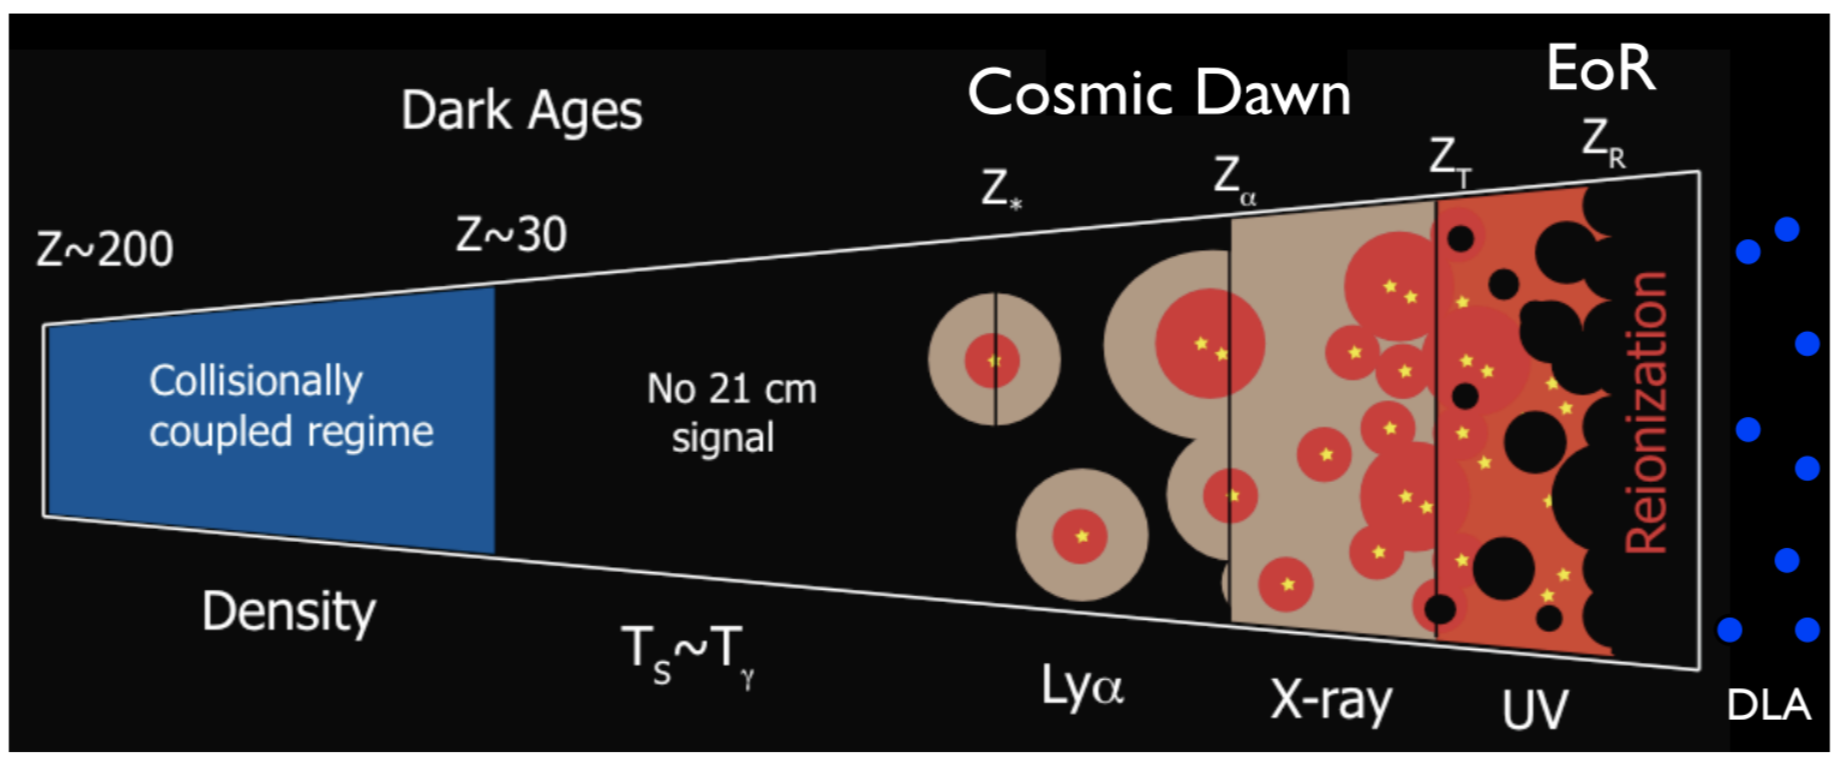
\includegraphics[width=16cm]{figures/cosmology/21cm_schematic.png}
    \centering
    \caption{\footnotesize{Cartoon of the different phases of the $21\,{\rm cm}$ signal. The signal transitions from an early phase of collisional coupling to a later phase of Ly$\alpha$ coupling through a short period where there is little signal. Fluctuations after this phase are dominated successively by spatial variation in the Ly$\alpha$, X-ray, and ionizing UV radiation backgrounds. After reionization is complete there is a residual signal from neutral hydrogen in galaxies. Figure taken from Ryden (2006).}}
    \label{fig:21cmschematic}
\end{figure}

{\noindent}Collisions between different particles may induce spin-flips in a hydrogen atom and dominate the coupling in the early Universe where the gas density is high. Three main channels are available: collisions between two hydrogen atoms and collisions between a hydrogen atom and an electron or a proton. The collisional coupling for a species is

\begin{align*}
    x_c^i \equiv \frac{C_{10}}{A_{10}}\frac{T_*}{T_\gamma} = \frac{n_ik_{10}^i}{A_{10}}\frac{T_*}{T_\gamma},
\end{align*}

{\noindent}where $C_{10}$ is the collisional excitation rate, $k_{10}^i$ is the specific rate coefficient for spin de-excitation by collisions with species $i$ (in units of $cm^3s^{-1}$).

{\noindent}The total collisional coupling coefficient can be written as

\begin{align*}
    x_c &= x_c^\mathrm{HH} + x_c^\mathrm{eH} + x_c^\mathrm{pH} \\
        &= \frac{T_*}{A_{10}T_\gamma} \left[k_{1-0}^\mathrm{HH}(T_k)n_\mathrm{H}+k_{1-0}^{e\mathrm{H}}(T_k)n_e+k_{1-0}^{p\mathrm{H}}(T_k)n_p\right] ~ [{\rm dimensionless}],
\end{align*}

{\noindent}where $k_{1-0}^\mathrm{HH}$ is the scattering rate between hydrogen atoms, $k_{1-0}^{e\mathrm{H}}$ is the scattering rate between hydrogen atoms and electrons, and $k_{1-0}^{p\mathrm{H}}$ is the scattering rate between hydrogen atoms and protons.

{\noindent}We may express the $21\,{\rm cm}$ brightness temperature as a function of four variables $T_b=T_b(T_k,x_i,J_\alpha,n_\mathrm{H})$, where $x_i$ is the volume-averaged ionized fraction of hydrogen and $J_\alpha$ is the Ly$\alpha$ specific flux. In calculating the $21\,{\rm cm}$ signal, we require a model for the global evolution of and fluctuations in these quantities. Before looking at the evolution of the signal quantitatively, we will first outline the basic picture to delineate the most important phases.

{\noindent}An important feature of $T_b$ is that its dependence on each of these quantities saturates at some point, for example once the Ly$\alpha$ flux is high enough the spin and kinetic gas temperatures become tightly coupled and further variation in $J_\alpha$ becomes irrelevant to the details of the signal. This leads to conceptually separate regimes where variation in only one of the variables dominating fluctuations in the signal. These different regimes can be seen in Figure \ref{fig:21cmannotated} and are shown in schematic form in Figure \ref{fig:21cmschematic}.

% --------------------------------------------------------------
%
%                           17. 
%
% --------------------------------------------------------------

\newpage
\subsection{Question 17}

What is the difference between scalar and tensor modes of perturbation in the early Universe, and how can you detect their presence?

\subsubsection{Short answer}

Scalar modes are density perturbations at the surface of last scattering which form gravitational instabilities. These seed temperature fluctuations in the CMB as well as E-mode polarization. In contrast, tensor modes are known as gravitational waves which cause shearing of the spacetime metric (compression in one direction and stretching in the other) These seed not only temperature fluctuations and E-mode polarization but also B-mode polarization. These modes do not damp out the way that scalar modes do. 

\subsubsection{Additional context}

{\noindent}Scalars, vectors, and tensors generate distinct patterns in the polarization of the CMB. However, although they separate cleanly into $m=0,\pm1,\pm2$ polarization patterns for a single plane wave perturbation in the coordinate system referenced to $\bm{k}$, in general there will exist a spectrum of fluctuations each with a different $\bm{k}$. Therefore the polarization pattern on the sky does not separate into $m=0,\pm1,\pm2$ modes. In fact, assuming statistical isotropy, one expects the ensemble averaged power for each multipole $\ell$ to be independent of $m$. Nonetheless, certain properties of the polarization patterns do survive superposition of the perturbations: in particular, its parity and its correlation with the temperature fluctuations.

\begin{figure}[h]
    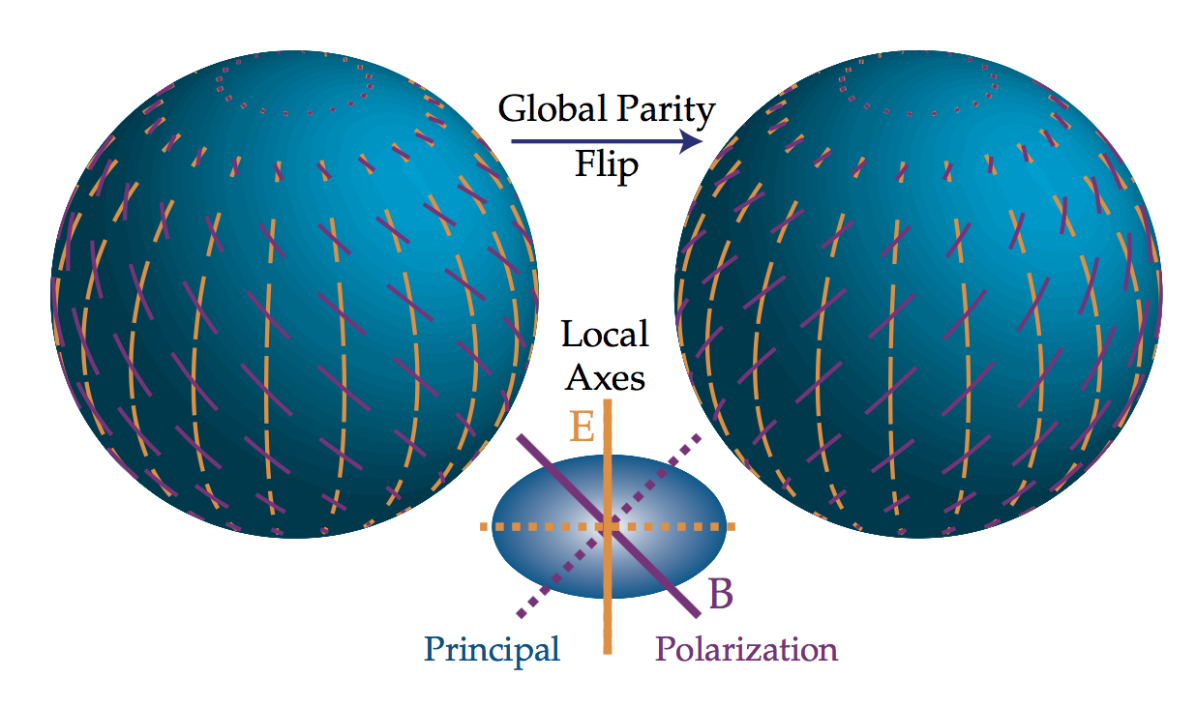
\includegraphics[width=16cm]{figures/cosmology/EBmodes.png}
    \centering
    \caption{\footnotesize{The electric ($E$) and magnetic ($B$) modes are distinguished by their behavior under a parity transformation $\bm{\hat{n}}\rightarrow\bm{\hat{n}}$. $E$-modes have $(-1)^\ell$ and $B$-modes have $(-1)^{\ell+1}$ parity; here ($\ell=2,m=0$), even and odd respectively. The local distinction between the two is that the polarization axis is aligned with the principle axes of the polarization amplitude for $E$ and crossed with them for $B$. Dotted lines represent a sign reversal in the polarization. Image taken from Hu \& White (1997).}}
    \label{fig:ebmodes}
\end{figure}

{\noindent}\textbf{Scalar (compressible) perturbations}: The most commonly considered and familiar types of perturbations are \textbf{scalar modes}. These modes represent perturbations in the (energy) density of the cosmological fluid(s) at last scattering and are the only fluctuations which can form structure though \textbf{gravitational instability}. Consider a single large-scale Fourier component of the fluctuation (i.e., for the photons, a single plane wave in the temperature perturbation). Over time, the temperature and gravitational potential gradients cause a bulk flow, or dipole anisotropy, of the photons. Both effects can be described by introducing an “effective” temperature

\begin{align*}
    \left(\frac{\Delta T}{T}\right)_\mathrm{eff} = \left(\frac{\Delta T}{T}\right) + \psi,
\end{align*}

{\noindent}where $\psi$ is the gravitational potential. Gradients in the effective temperature always create flows from hot to cold effective temperature. Formally, both pressure and gravity act as sources of the momentum density of the fluid in a combination that is exactly the effective temperature for a relativistic fluid.

{\noindent} To avoid confusion, let us explicitly consider the case of adiabatic fluctuations, where initial perturbations to the density imply potential fluctuations that dominate at large scales. Here gravity overwhelms pressure in overdense regions causing matter to flow towards density peaks initially. Nonetheless, overdense regions are effectively cold initially because photons must climb out of the potential wells they create and hence lose energy in the process. Though flows are established from cold to hot temperature regions on large scales, they still go from hot to cold effective temperature regions. This property is true more generally of our adiabatic assumption: we hereafter refer only to effective temperatures to keep the argument general.

\begin{figure}[t!]
    \centering
    \vspace{-1cm}
    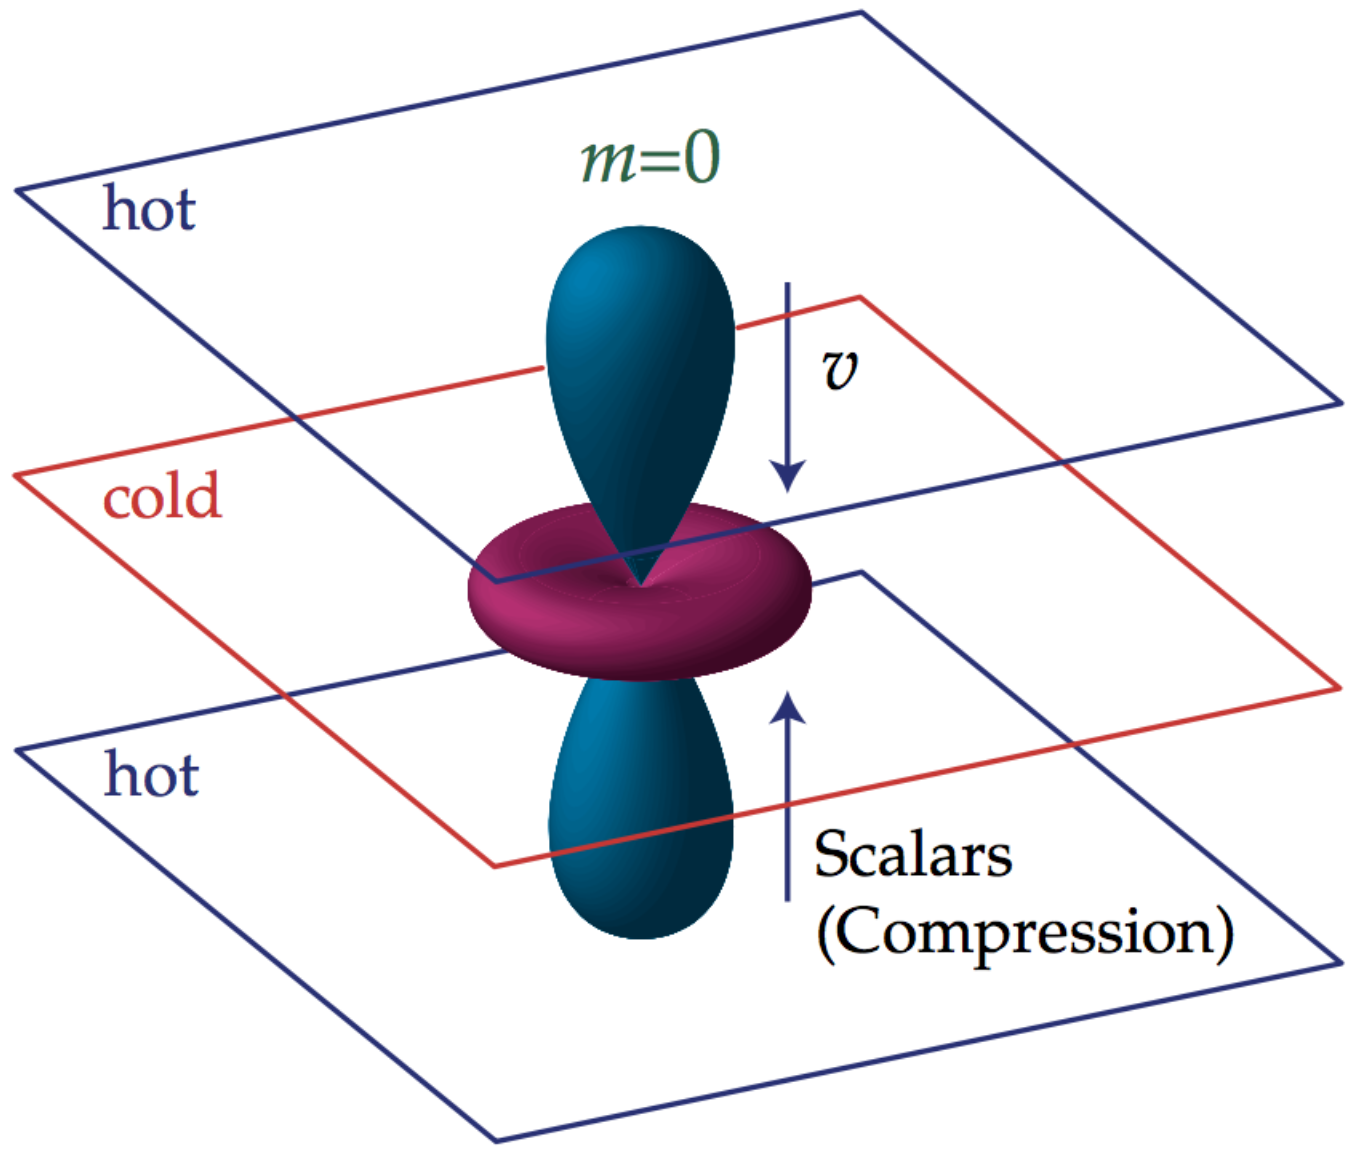
\includegraphics[width=8cm]{figures/cosmology/ScalarQuadrupole.png}\\
    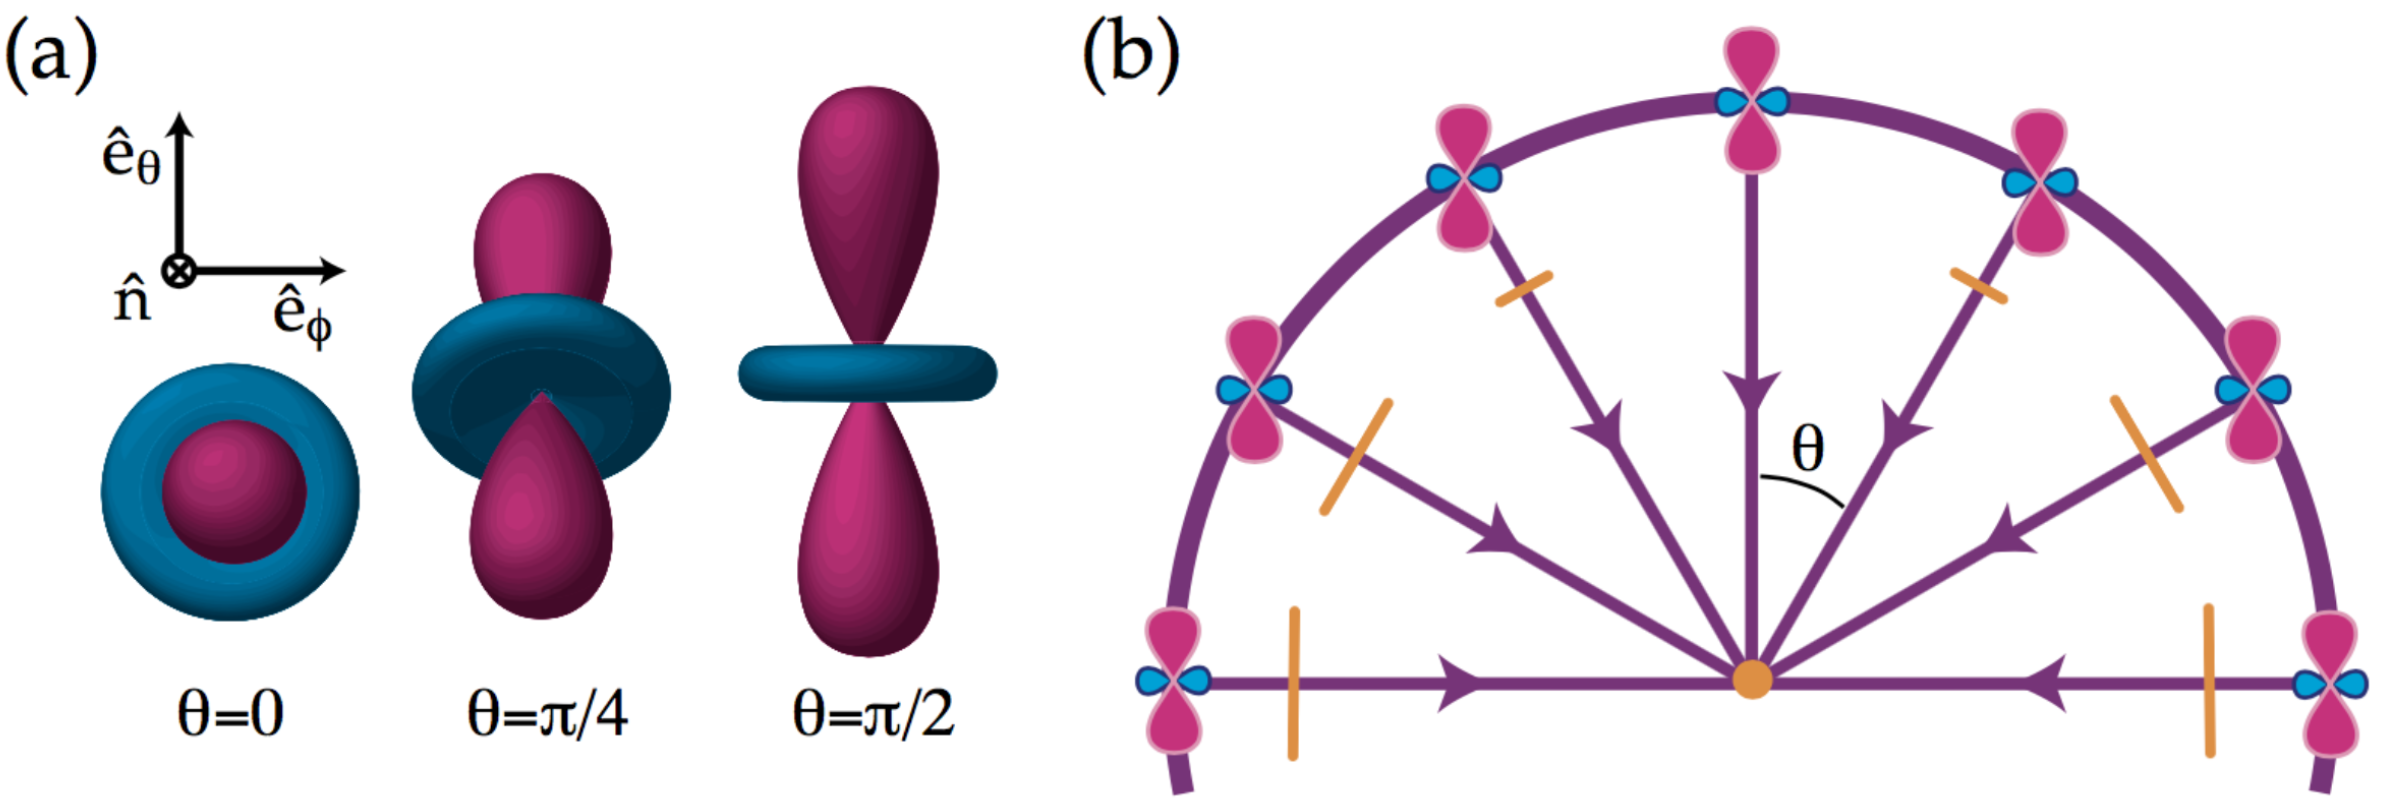
\includegraphics[width=15cm]{figures/cosmology/QuadrupolarAnisotropies.png}\\
    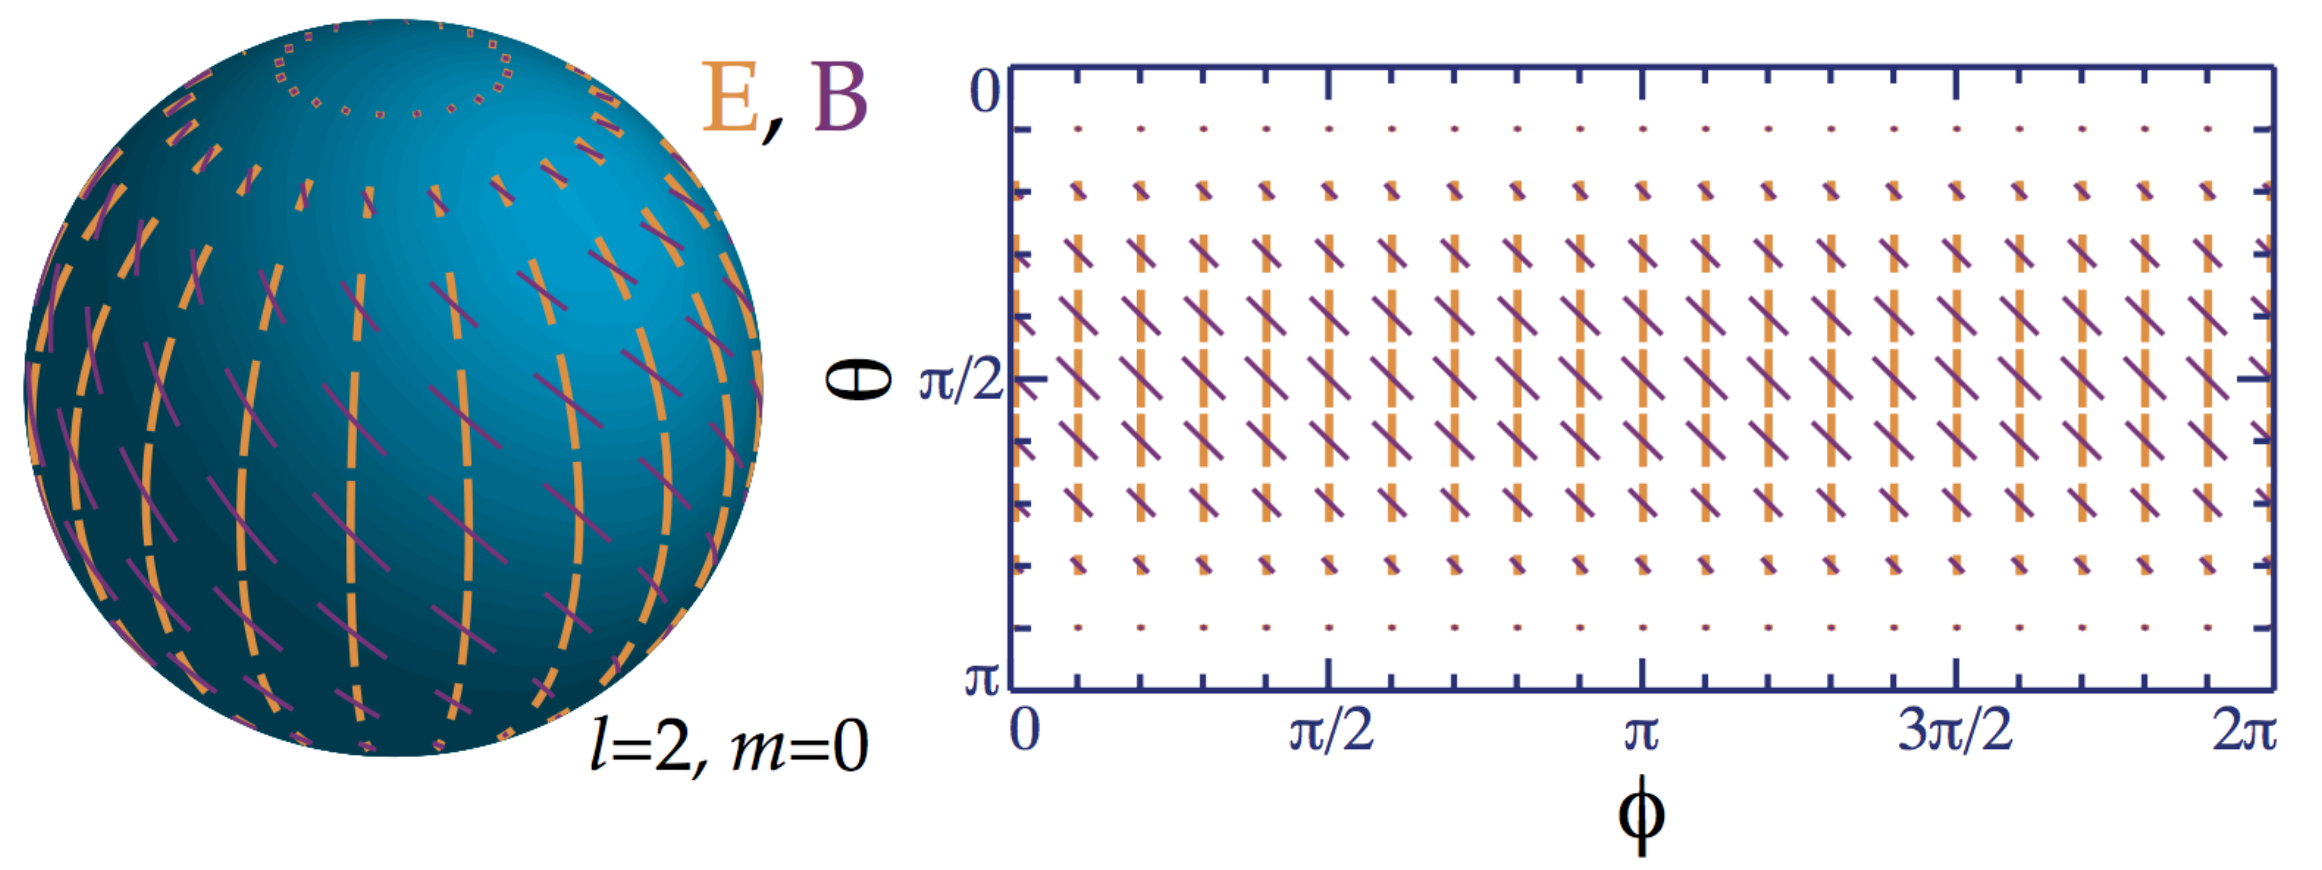
\includegraphics[width=15cm]{figures/cosmology/ScalarPattern.png}
    \caption{\footnotesize{\textbf{(Top)} The scalar quadrupole moment ($\ell=2,m=0$). Flows from hot (blue) regions into cold (red), $\bm{v}\parallel\bm{k}$, produce the azimuthally symmetric pattern $Y_2^0$ depicted here. \textbf{(Middle)} The transformation of quadrupole anisotropies into linear polarization. (a) The orientation of the quadrupole moment with respect to the scattering direction $\bm{\hat{n}}$ determines the sense and magnitude of the polarization. It is aligned with the cold (red, long) lobe in the $\bm{\hat{e}}_\theta\times\bm{\hat{e}}_\phi$ tangent plane. (b) In spherical coordinates where $\bm{\hat{n}}\cdot\bm{\hat{k}}=\cos\theta$, the polarization points north-south ($Q$) with magnitude varying as $\sin^2Ξ$ for scalar fluctuations. \textbf{(Bottom)} Polarization pattern for $\ell=2,m=0$, note the azimuthal symmetry. The scattering of a scalar $m=0$ quadrupole perturbation generates the electric $E$ (yellow, thick lines) pattern on the sphere. Its rotation by $45^\circ$ represents the orthogonal magnetic $B$ (purple, thin lines) pattern. Animation (available at \href{http://www.sns.ias.edu/∌whu/polar/scalaran.html}{http://www.sns.ias.edu/∌whu/polar/scalaran.html}): as the line of sight $\bm{\hat{n}}$ changes, the lobes of the quadrupole rotate in and out of the tangent plane. The polarization follows the orientation of the colder (red) lobe in the tangent plane. Images taken from Hu \& White (1997).}}
    \label{fig:scalar}
\end{figure}

{\noindent}Let us consider the quadrupole component of the temperature pattern seen by an observer located in a trough of a plane wave. The azimuthal symmetry in the problem requires that $\bm{v}\parallel\bm{k}$ and hence the flow is irrotational $\nabla\times\bm{v}=0$. Because hotter photons from the crests flow into the trough from the $\pm k$ directions while cold photons surround the observer in the plane, the quadrupole pattern seen in a trough has an $m = 0$,

\begin{align*}
    Y_2^0 \propto 3\cos^2\theta-1,
\end{align*}

{\noindent}structure with angle $\bm{\hat{n}\cdot\hat{k}}=\cos\theta$ (see top of Figure \ref{fig:scalar}). The opposite effect occurs at the crests, reversing the sign of the quadrupole but preserving the $m=0$ nature in its local angular dependence. The full effect is thus described by a local quadrupole modulated by a plane wave in space, $-Y_2^0(\bm{\hat{n}})\exp(i\bm{k}\cdot\bm{x})$, where the sign denotes the fact that photons flowing into cold regions are hot. This infall picture must be modified slightly on scales smaller than the sound horizon where pressure plays a role, however the essential property that the flows are parallel to $\bm{\hat{k}}$ and thus generate an $m=0$ quadrupole remains true.

{\noindent}The sense of the quadrupole moment determines the polarization pattern through Thomson scattering. Recall that polarized scattering peaks when the temperature varies in the direction orthogonal to $\bm{\hat{n}}$. Consider then the tangent plane $\bm{\hat{e}}_\theta\times\bm{\hat{e}}_\phi$ with normal $\bm{\hat{n}}$. This may be visualized in an angular ``lobe'' diagram such as the top of Figure \ref{fig:scalar} as a plane which passes through the ``origin'' of the quadrupole pattern perpendicular to the line of sight. The polarization is maximal when the hot and cold lobes of the quadrupole are in this tangent plane, and is aligned with the component of the colder lobe which lies in the plane. As $\theta$ varies from $0$ to $\pi/2$ (pole to equator) the temperature differences in this plane increase from zero (see middle of Figure \ref{fig:scalar} a). The local polarization at the crest of the temperature perturbation is thus purely in the N-S direction tapering off in amplitude toward the poles (see middle of Figure \ref{fig:scalar} b). This pattern represents a pure $Q$-field on the sky whose amplitude varies in angle as an $\ell=2,m=0$ tensor or spin-$2$ spherical harmonic (Newman \& Penrose, 1966)

\begin{align*}
    Q=\sin^2\theta,~~~~~U=0.
\end{align*}

{\noindent}In different regions of space, the plane wave modulation of the quadrupole can change the sign of the polarization, but not its sense.

{\noindent}This pattern (bottom of Figure \ref{fig:scalar}, thick lines) is of course not the only logical possibility for an $\ell=2,m=0$ polarization pattern. Its rotation by $45^\circ$ is also a valid configuration (thin lines). This represents a pure NW-SE (and by sign reversal NE-SW), or $U$-polarization pattern (a distinction between the two patterns being electric and magnetic modes).

{\noindent}\textbf{Vector (vortical) perturbations}: \textbf{Vector perturbations} represent vortical motions of the matter, where the velocity field $\bm{v}$ obeys $\nabla\cdot\bm{v}=0$ and $\nabla\times\bm{v}\neq0$, similar to ``eddies'' in water. There is no associated density perturbation, and the vorticity is damped by the expansion of the Universe as are all motions that are not enhanced by gravity. However, the associated temperature fluctuations, once generated, do not decay as both $\Delta T$ and $T$ scale similarly with the expansion. For a plane wave perturbation, the velocity field $\bm{v}\perp\bm{k}$ with direction reversing in crests and troughs (see top of Figure \ref{fig:vector}). The radiation field at these extrema possesses a dipole pattern due to the Doppler shift from the bulk motion. Quadrupole variations vanish here but peak between velocity extrema. To see this, imagine sitting between crests and troughs. Looking up toward the trough, one sees the dipole pattern projected as a hot and cold spot across the zenith; looking down toward the crest, one sees the projected dipole reversed. The net effect is a quadrupole pattern in temperature with $m\pm1$

\begin{align*}
    Y_2^{\pm1}\propto\sin\theta\cos\theta\mathrm{e}{\pm i\phi}.
\end{align*}

\begin{figure}[t!]
    \centering
    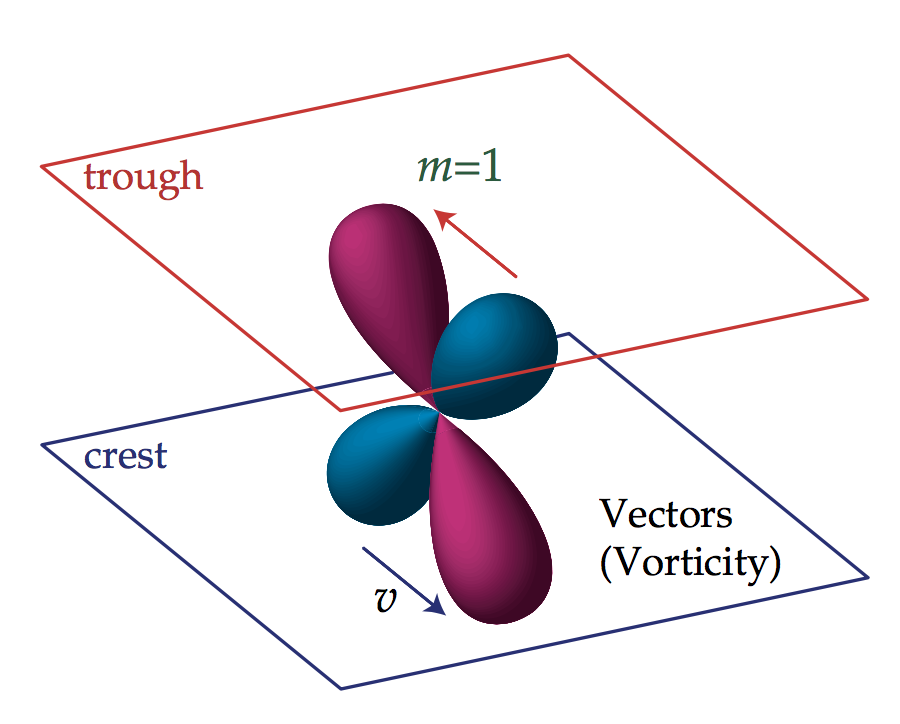
\includegraphics[width=8cm]{figures/cosmology/VectorQuadrupole.png}
    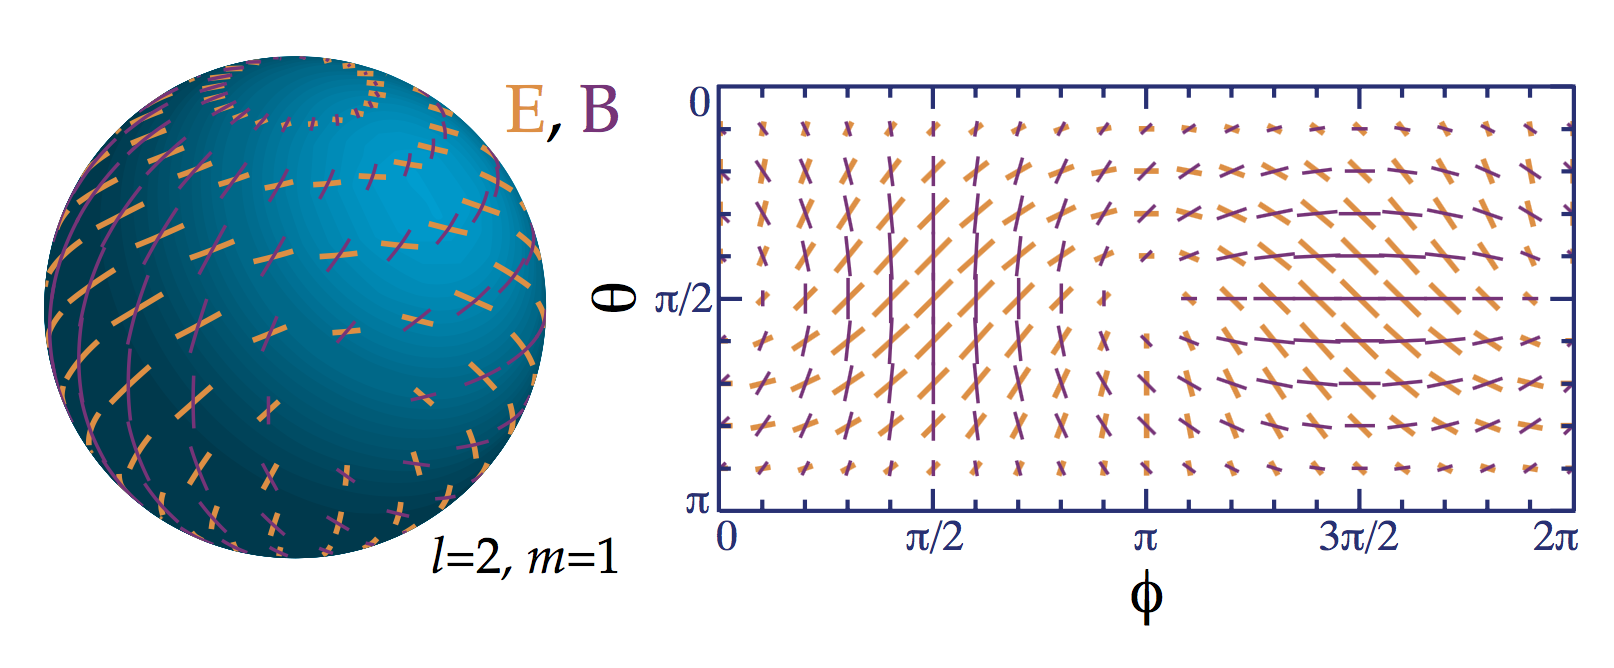
\includegraphics[width=15cm]{figures/cosmology/VectorPattern.png}
    \caption{\footnotesize{\textbf{(Top)} The vector quadrupole moment ($l=2,m=1$). Since $\bm{v}\perp\bm{k}$, the Doppler effect generates a quadrupole pattern with lobes $45^\circ$ from $\bm{v}$ and $\bm{k}$ that is spatially out of phase (interplane peaks) with $v$. \textbf{(Bottom)} Polarization pattern for $\ell=2,m=1$. The scattering of a vector ($m=1$) quadrupole perturbation generates the $E$ pattern (yellow, thick lines) as opposed to the $B$, (purple, thin lines) pattern. Animation (available at \href{http://www.sns.ias.edu/∌whu/polar/vectoran.html}{http://www.sns.ias.edu/∌whu/polar/vectoran.html}): same as for scalars. Images taken from Hu \& White (1997).}}
    \label{fig:vector}
\end{figure}

{\noindent}The lobes are oriented at $45^\circ$ from $k$ and $v$ since the line
of sight velocity vanishes along $k$ and at $90$ degrees to $k$ here. The latter follows since midway between the crests and troughs $v$ itself is zero. The full quadrupole distribution is therefore described by $-iY_2^{\pm1}(\bm{\hat{n}})\exp(i\bm{k}\cdot\bm{x})$, where $i$ represents the spatial phase shift of the quadrupole with respect to the velocity.

{\noindent}Thomson scattering transforms the quadrupole temperature anisotropy into a local polarization field as before. Again, the pattern may be visualized from the intersection of the tangent plane to $\bm{\hat{n}}$ with the lobe pattern of the top of Figure \ref{fig:vector}. At the equator ($\theta=\pi/2$), the lobes are oriented $45^\circ$ from the line of sight $\bm{\hat{n}}$ and rotate into and out of the tangent plane with $\phi$. The polarization pattern here is a pure $U$-field which varies in magnitude as $\sin\phi$. At the pole $\theta=0$, there are no temperature variations in the tangent plane so the polarization vanishes. Other angles can equally well be visualized by viewing the quadrupole pattern at different orientations given by $\bm{\hat{n}}$.

{\noindent}The full $\ell=2,m=1$ pattern,

\begin{align*}
    Q=-\sin\theta\cos\theta\mathrm{e}^{i\phi},~~~~~U=-i\sin\theta\mathrm{e}^{i\phi}
\end{align*}

{\noindent}is displayed explicitly in the bottom of Figure \ref{fig:vector}. Note that the pattern is dominated by $U$-contributions especially near the equator.

{\noindent}\textbf{Tensor (gravitational wave) perturbations}:

{\noindent}Tensor fluctuations are transverse-traceless perturbations to the metric, which can be viewed as gravitational waves. A plane gravitational wave perturbation represents a quadrupolar ``stretching'' of space in the plane of the perturbation (see Figure \ref{fig:tensor}). As the wave passes or its amplitude changes, a circle of test particles in the plane is distorted into an ellipse whose semi-major axis $\rightarrow$ semi-minor axis as the spatial phase changes from crest $\rightarrow$ trough (see the top of Figure \ref{fig:tensor}, yellow ellipses). Heuristically, the accompanying stretching of the wavelength of photons produces a quadrupolar temperature variation with an $m=\pm2$ pattern

\begin{align*}
    Y_2^{\pm2}\propto\sin^2\theta\mathrm{e}^{\pm2i\phi}
\end{align*}

{\noindent}in the coordinates defined by $\bm{\hat{k}}$.

\begin{figure}[t!]
    \centering
    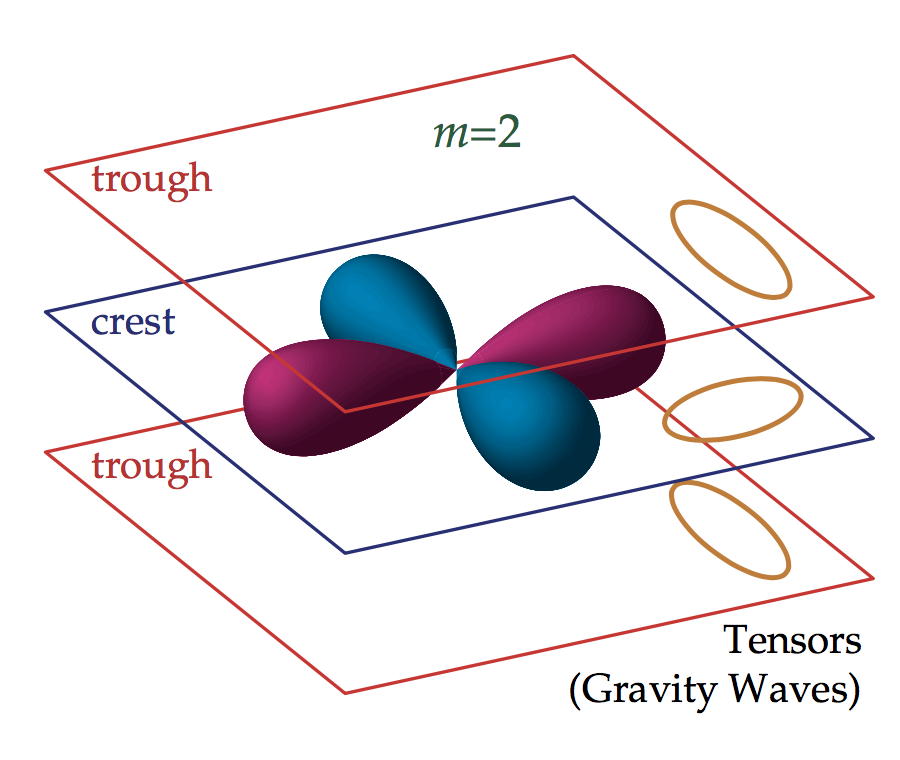
\includegraphics[width=8cm]{figures/cosmology/TensorQuadrupole.png}
    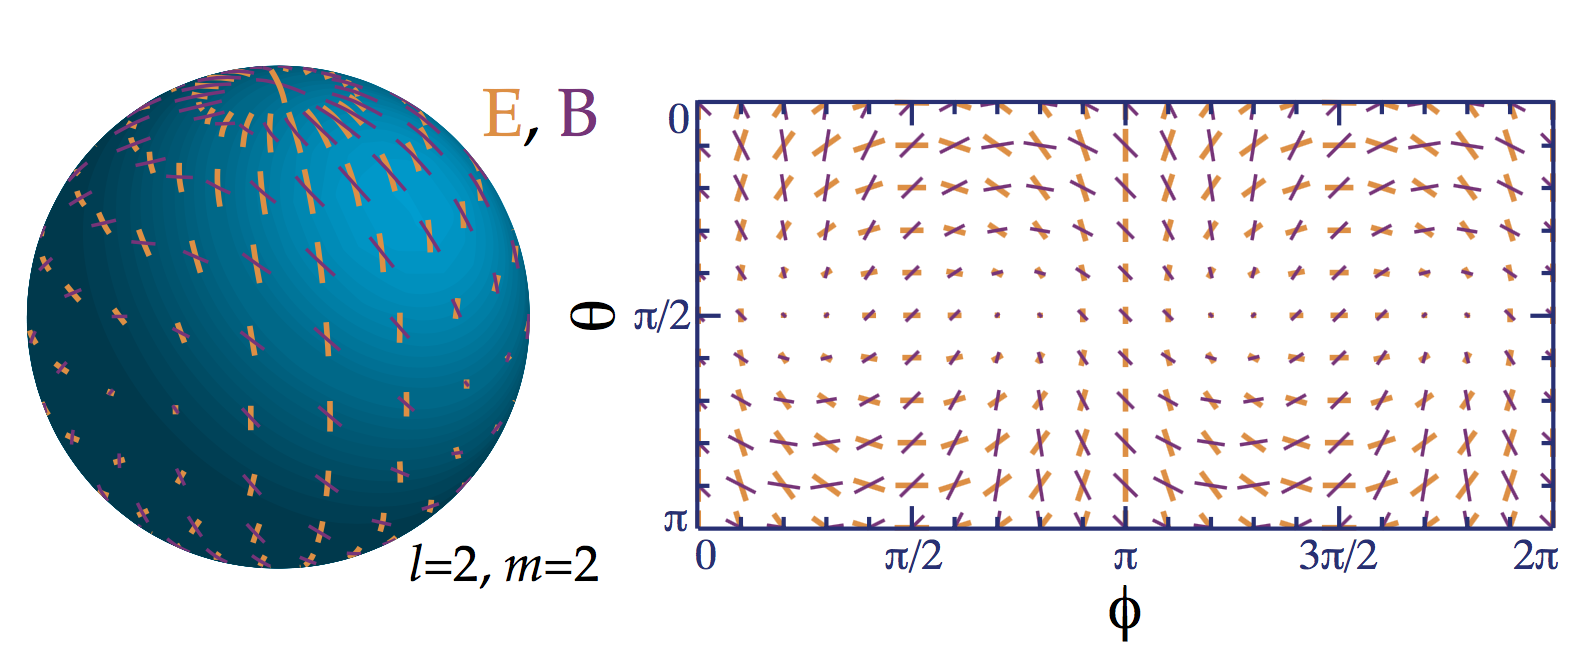
\includegraphics[width=15cm]{figures/cosmology/TensorPattern.png}
    \caption{\footnotesize{\textbf{(Top)} The tensor quadrupole moment $(m=2)$. Since gravity waves distort space in the plane of the perturbation, changing a circle of test particles into an ellipse, the radiation acquires an $m=2$ quadrupole moment. \textbf{(Bottom)} Polarization pattern for $\ell=2,m=2$. Scattering of a tensor $m=2$ perturbation generates the $E$ (yellow, thick lines) pattern as opposed to the $B$ (purple, thin lines) pattern. Animation (available at \href{http://www.sns.ias.edu/∌whu/polar/vectoran.html}{http://www.sns.ias.edu/∌whu/polar/vectoran.html}): same as for scalars. Images taken from Hu \& White (1997).}}
    \label{fig:tensor}
\end{figure}

{\noindent}Thomson scattering again produces a polarization pattern from the quadrupole anisotropy. At the equator, the quadrupole pattern intersects the tangent ($\bm{\hat{e}}_\theta\times\bm{\hat{e}}_\phi$) plane with hot and cold lobes rotating in and out of the $\bm{\hat{e}}_\phi$ direction with the azimuthal angle $\phi$. The polarization pattern is therefore purely $Q$ with a $\cos(2\phi)$ dependence. At the pole, the quadrupole lobes lie completely in the polarization plane and produces the maximal polarization unlike the scalar and vector cases. The full pattern,

\begin{align*}
    Q=(1+\cos^2\theta)\mathrm{e}^{2i\phi}~[{\rm Jy}], ~~~~~U=-2i\cos\theta\mathrm{e}^{2i\phi}~[{\rm Jy}],
\end{align*}

{\noindent}is shown in the bottom of Figure \ref{fig:tensor} (real part). Note that $Q$ and $U$ are present in nearly equal amounts for the tensors.

{\noindent}\textit{Electric and Magnetic Modes}:

{\noindent}Any polarization pattern on the sky can be separated into ``electric'' ($E$) and ``magnetic'' ($B$) components. This decomposition is useful both observationally and theoretically. There are two equivalent ways of viewing the modes that reflect their global and local properties respectively. The nomenclature reflects the global property. Like multipole radiation, the harmonics of an $E$-mode have $(-1)^\ell$ parity on the sphere, whereas those of a $B$-mode have $(-1)^{\ell+1}$ parity. Under $\bm{\hat{n}}\rightarrow\bm{\hat{n}}$, the $E$-mode thus remains unchanged for even $\ell$, whereas the $B$-mode changes sign as illustrated for the simplest case $\ell=2,m=0$ in Figure \ref{fig:ebmodes} (recall that a rotation by $90^\circ$ represents a change in sign). Note that the $E$ and $B$ multipole patterns are $45^\circ$ rotations of each other, (i.e. $Q\rightarrow U$ and $U\rightarrow-Q$). Since this parity property is obviously rotationally invariant, it will survive integration over $\bm{\hat{k}}$.

{\noindent}The local view of $E$- and $B$-modes involves the second derivatives of the polarization amplitude (second derivatives because polarization is a tensor or spin-$2$ object). In much the same way that the distinction between electric and magnetic fields in electromagnetism involves vanishing of gradients or curls (i.e., first derivatives) for the polarization there are conditions on the second (covariant) derivatives of $Q$ and $U$. For an $E$-mode, the difference in second (covariant) derivatives of $U$ along $\bm{\hat{e}}_\theta$ and $\bm{\hat{e}}_\phi$ vanishes as does that for $Q$ along $\bm{\hat{e}}_\theta+\bm{\hat{e}}_\phi$ and $\bm{\hat{e}}_\theta-\bm{\hat{e}}_\phi$. For a $B$-mode, $Q$ and $U$ are interchanged. Recalling that a $Q$-field points in the $\bm{\hat{e}}_\theta$ or $\bm{\hat{e}}_\phi$ direction and a $U$-field in the crossed direction, we see that the Hessian or curvature matrix of the polarization amplitude has principle axes in the same sense as the polarization for $E$ and $45^\circ$ crossed with it for $B$ (see Figure \ref{fig:ebmodes}). Stated another way, near a maximum of the polarization (where the first derivative vanishes) the direction of greatest change in the polarization is parallel/perpendicular and at $45^\circ$ degrees to the polarization in the two cases.

{\noindent}The distinction is best illustrated with examples. Take the simplest case of $\ell=2,m=0$ where the $E$-mode is a $Q=\sin^2\theta$ field and the $B$-mode is a $U=\sin^2\theta$ field (see the bottom of Figure \ref{fig:scalar}). In both cases, the major axis of the curvature lies in the $\bm{\hat{e}}_\theta$ direction. For the $E$-mode, this is in the same sense; for the $B$-mode it is crossed with the polarization direction. The same holds true for the $m=1,2$ modes as can be seen by inspection of the bottom of Figure \ref{fig:vector} and the bottom of Figure \ref{fig:tensor}.

\begin{figure}[t!]
    \centering
    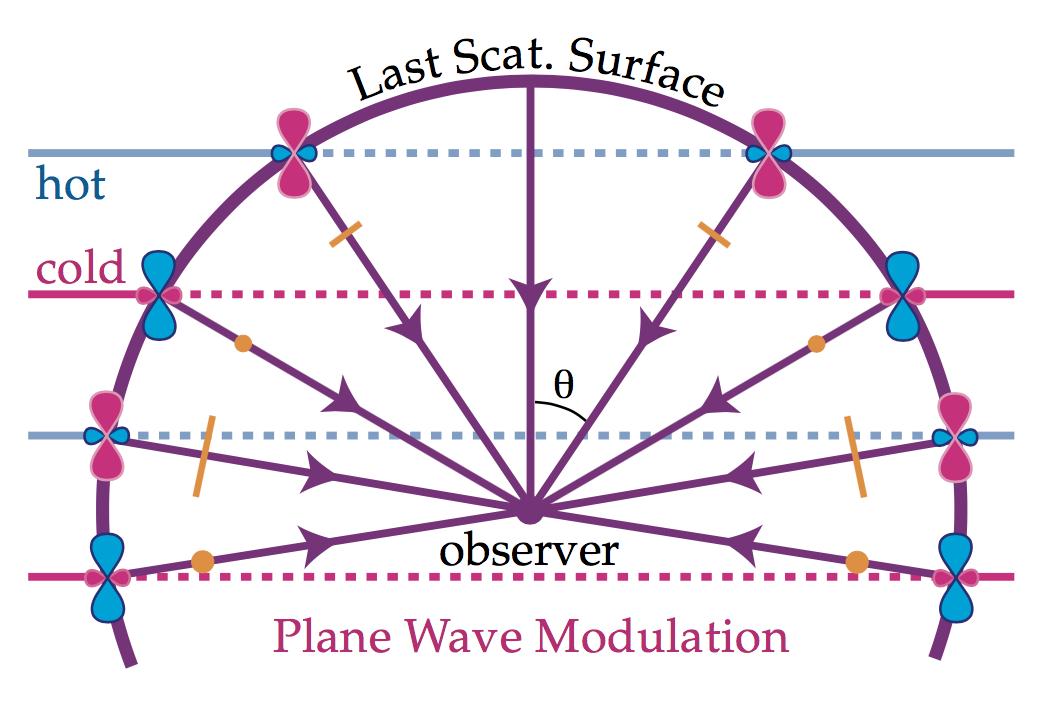
\includegraphics[width=10cm]{figures/cosmology/CMBquad.png}
    \caption{\footnotesize{Modulation of the local pattern in the bottom of Figure \ref{fig:scalar} by plane wave fluctuations on the last scattering surface. Yellow points represent polarization out of the plane with magnitude proportional to sign. The plane wave modulation changes the amplitude and sign of the polarization but does not mix $Q$ and $U$. Modulation can mix $E$ and $B$ however if $U$ is also present. Image taken from Hu \& White (1997).}}
    \label{fig:cmbquad}
\end{figure}

{\noindent}Thomson scattering can only produce an $E$-mode locally since the spherical harmonics that describe the temperature anisotropy have $(-1)^\ell$ electric parity. In the tops of Figures \ref{fig:scalar}, \ref{fig:vector}, and \ref{fig:tensor}, the $\ell=2,m=0,1,2$ $E$-mode patterns are shown in yellow. The $B$-mode represents these patterns rotated by $45^\circ$ and are shown in purple and cannot be generated by scattering. In this way, the scalars, vectors, and tensors are similar in that scattering produces a local $\ell=2$ $E$-mode only.

{\noindent}However, the pattern of polarization on the sky is not simply this local signature from scattering but is modulated over the last scattering surface by the plane wave spatial dependence of the perturbation (compare the bottom of Figure \ref{fig:scalar} and \ref{fig:cmbquad}). The modulation changes the amplitude, sign, and angular structure of the polarization but not its nature (e.g. a $Q$-polarization remains Q). Nonetheless, this modulation generates a $B$-mode from the local $E$-mode pattern.

{\noindent}The reason why this occurs is best seen from the local distinction between $E$ and $B$-modes. Recall that $\mathbf{E}$\textbf{-modes} have polarization amplitudes that change parallel or perpendicular to, and $\mathbf{B}$\textbf{-modes} in directions $45^\circ$ away from, the polarization direction. On the other hand, plane wave modulation always changes the polarization amplitude in the direction $\bm{\hat{k}}$ or N-S on the sphere. Whether the resultant pattern possesses $E$ or $B$-contributions depends on whether the local polarization has $Q$ or $U$-contributions.

{\noindent}For scalars, the modulation is of a pure $Q$-field and thus its $E$-mode nature is preserved (Kamionkowski et al. 1997; Zaldarriaga \& Seljak 1997). For the vectors, the $U$-mode dominates the pattern and the modulation is crossed with the polarization direction. Thus vectors generate mainly $B$-modes for short wavelength fluctuations (Hu \& White 1997). For the tensors, the comparable $Q$ and $U$ components of the local pattern imply a more comparable distribution of $E$ and $B$ modes at short wavelengths (see Figure \ref{fig:polpatterns}a).

\begin{figure}[t!]
    \centering
    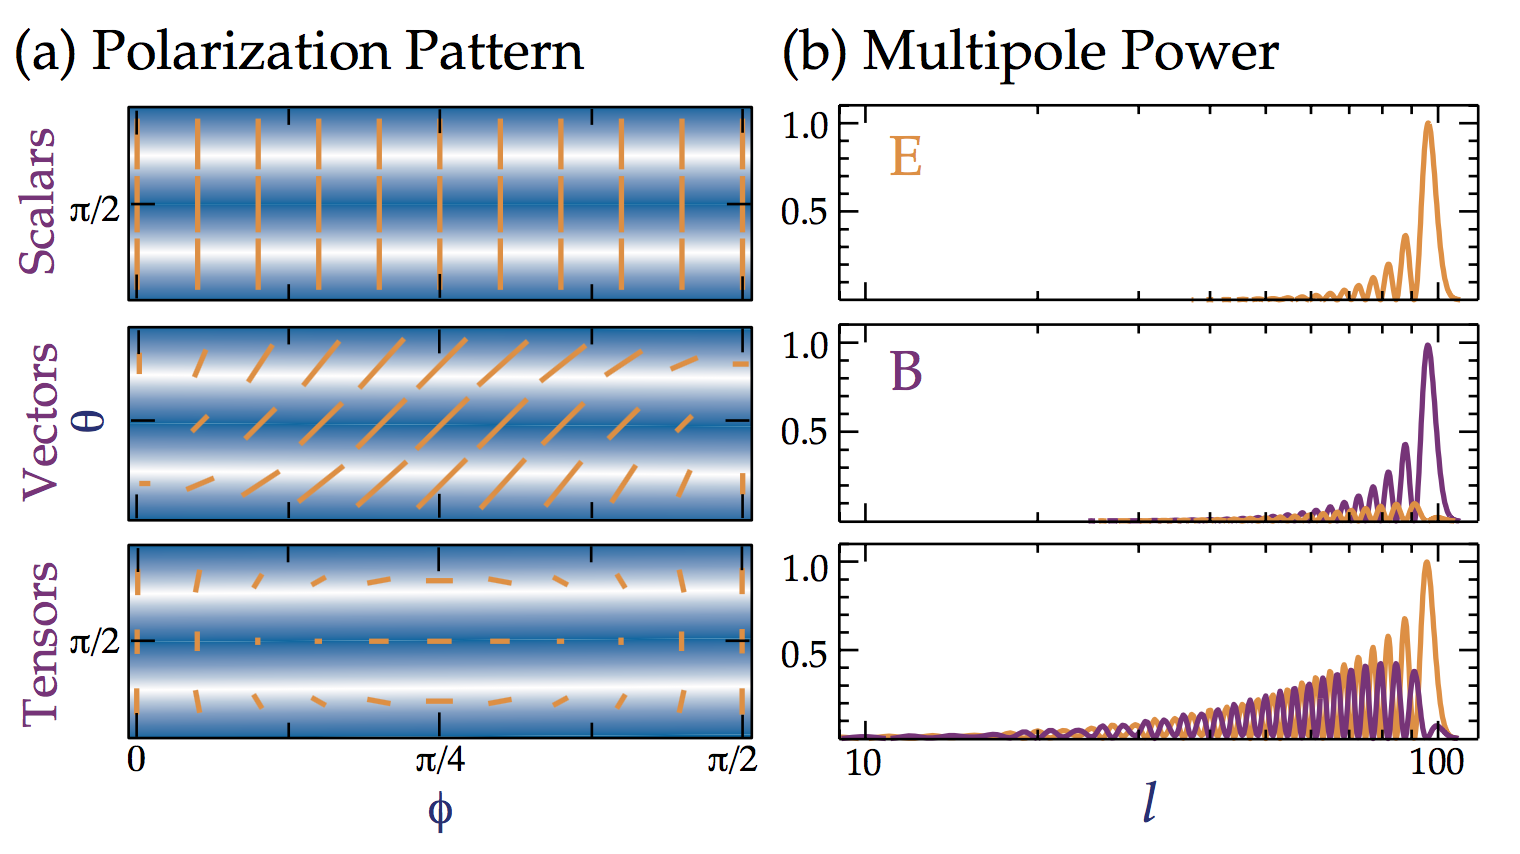
\includegraphics[width=16cm]{figures/cosmology/PolPatterns.png}
    \caption{\footnotesize{The $E$ and $B$ components of a plane wave perturbation. (a) Modulation of the local $E$-quadrupole pattern (yellow) from scattering by a plane wave. Modulation in the direction of (or orthogonal to) the polarization generates an $E$-mode with higher $\ell$; modulation in the crossed ($45^\circ$) direction generates a $B$-mode with higher $\ell$. Scalars generate only $E$-modes, vectors mainly $B$-modes, and tensors comparable amounts of both. (b) Distribution of power in a single plane wave with $kr=100$ in multipole $\ell$ from the addition of spin and orbital angular momentum. Features in the power spectrum can be read directly off the pattern in (a). Image taken from Hu \& White (1997).}}
    \label{fig:polpatterns}
\end{figure}

{\noindent}These qualitative considerations can be quantified by noting that plane wave modulation simply represent the addition of angular momentum from the plane wave ($Y_\ell^0$) with the local spin angular dependence. The result is that plane wave modulation takes the $\ell=2$ local angular dependence to higher $\ell$ (smaller angles) and splits the signal into $E$ and $B$ components with ratios which are related to Clebsch-Gordan coefficients. At short wavelengths, these ratios are $B/E=0$, $6$, $8/13$ in power for scalars, vectors, and tensors (see Figure \ref{fig:polpatterns}b and Hu \& White 1997).

{\noindent}The distribution of power in multipole $\ell$-space is also important. Due to projection, a single plane wave contributes to a range of angular scales  $\ell\lesssim kr$ where $r$ is the comoving distance to the last scattering surface. From Figure \ref{fig:cmbquad}, we see that the smallest angular, largest $\ell\approx kr$ variations occur on lines of sight $\bm{\hat{n}}\cdot\bm{\hat{k}}=0$ or $\theta=\pi/2$ though a small amount of power projects to $\ell\ll kr$ as $\theta\rightarrow0$. The distribution of power in multipole space of Figure \ref{fig:polpatterns}b can be read directly off the local polarization pattern. In particular, the region near $\theta=\pi/2$ shown in Figure \ref{fig:polpatterns}a determines the behavior of the main contribution to the polarization power spectrum.

{\noindent}The full power spectrum is of course obtained by summing these plane wave contributions with weights dependent on the source of the perturbations and the dynamics of their evolution up to last scattering. Sharp features in the $k$-power spectrum will be preserved in the multipole power spectrum to the extent that the projectors in Figure \ref{fig:polpatterns}b approximate delta functions. For scalar $E$-modes, the sharpness of the projection is enhanced due to strong $Q$-contributions near $\theta=\pi/2$ $(\ell\sim kr)$ that then diminish as $\theta\rightarrow0$ $(\ell\ll kr)$. The same enhancement occurs to a lesser extent for vector $B$-modes due to $U$ near $\pi/2$ and tensor $E$-modes due to $Q$ there. On the other hand, a suppression occurs for vector $E$ and tensor $B$-modes due to the absence of $Q$ and $U$ at $\pi/2$ respectively. These considerations have consequences for the sharpness of features in the polarization power spectrum, and the generation of asymptotic ``tails'' to the polarization spectrum at low-$\ell$ (see Hu \& White 1997) .

\subsubsection{Follow-up Questions}

\begin{itemize}
    \item What physically causes the polarization of the CMB in these modes?
    \item Have we detected scalar modes yet? What about tensor modes?
    \item How does this relate to BICEP's detection of primordial B-modes?
    \item What are some challenges to these detections?
    \item What are some foregrounds to these modes?
    \item If, say, both E- and B-modes were present in the CMB polarization, how might one disentangle them?
\end{itemize}

% --------------------------------------------------------------
%
%                           18. 
%
% --------------------------------------------------------------

\newpage
\subsection{Question 18}

What are the similarities and differences between the cosmic neutrino background and the cosmic microwave background?

\subsubsection{Short answer}

\begin{itemize}
    \item The CMB is from $\sim380,000$ years after the BB (or a redshift of $z\sim1100$), while the CNB is from $\sim1$ second after the BB.
    \item The CMB occurred when the Universe was $\sim1,000\,{\rm K}$ (or $\sim0.1\,{\rm eV}$) while that of the CNB was $\sim10^{10}\,{\rm K}$ (or $\sim1\,{\rm MeV}$).
    \item The expansion of the Universe has cooled the temperature of the CMB to $\sim2.7\,{\rm K}$ and the CNB to $\sim1.95\,{\rm K}$.
\end{itemize}

\subsubsection{Additional context}

Just as the CMB is a relic of the time when the Universe was opaque to photons, the CNB is a relic of the time when the Universe was hot and dense enough to be opaque to neutrinos. The number density of each of the three flavors of neutrinos ($\nu_e$, $\nu_\mu$, and $\nu_\tau$) has been calculated to be 3/11 times the number density of CMB photons. This means that at any moment, about twenty million cosmic neutrinos are zipping through your body.

{\noindent}The CMB yields information about our Universe at around $380,000$ years after the BB. Due to the weak interaction of the neutrinos with matter the CNB should give information about a much earlier time of our Universe, around one second after the Big Bang.

{\noindent}The CNB (often also called `relic neutrinos') decouples from matter about 1 second after the BB in the radiation dominated era at a temperature of $10^{10}\,{\rm K}\equiv1\,{\rm MeV}$. Today due to the expansion and cooling of the Universe the relic neutrino temperature is $1.95\,{\rm K}$ and the average neutrino density in the Universe is $340\,{\rm cm^{-3}}$ or $56\,\nu_e\,{\rm cm^{-3}}$.

{\noindent}The existence of a CNB (the analogue of the CMB) is a fundamental prediction of standard big bang cosmology. Up to now, the observational evidence for its existence is rather indirect and rests entirely on cosmological observations of, e.g., the light elemental abundances, the anisotropies in the CMB, and the large scale distribution of matter. All these measurements, however, probe the presence of relic neutrinos only at early stages in the cosmological evolution and, moreover, in a rather indirect way. The most promising laboratory search, based on neutrino capture on beta decaying nuclei, may be done in future experiments designed to measure the neutrino mass through decay kinematics.

{\noindent}Since the neutrinos interact with matter only by the weak interaction they decouple much earlier than the photons, which interact by the electromagnetic force. The decoupling of the neutrinos from matter is determined by the competition of the expansion rate of the Universe (Hubble parameter) and the interaction rate of the neutrinos with matter, occurring about 1 second after the BB.

{\noindent}Despite its successes, the standard model is known to be incomplete, and in at least one aspect, it directly conflicts with observations: according to the standard model, neutrinos should be massless. However, the Solar neutrino problem and its solution has shown this to be not the case: The (electron) neutrinos generated through nuclear fusion in the center of the Sun can escape, due to their small interaction cross section. These Solar neutrinos can be detected in (big!) terrestrial detectors. However, the measured rate of electron neutrinos from the Sun is only half as large as expected from Solar models. This Solar neutrino problem kept physicists and astrophysicists busy for decades. Its solution consists of a purely quantum-mechanical process, that of neutrino oscillations. It it possible that during its propagation, an electron neutrino transforms into a muon or tau neutrino, and back again. The existence of such oscillations was speculated for a long time, and provides a possible explanation for the missing rate of Solar electron neutrinos. Indeed, in 2001 the Sudbury Neutrino Observatory showed that neutrinos of all three flavors are received from the Sun, and that the sum of the rates of these neutrinos is compatible with the predicted rate from Solar models. In the meantime, these neutrino oscillation have also been observed in terrestrial experiments with neutrino beams.

{\noindent}Whereas neutrino oscillations are therefore well established today, they are in conflict with the Standard Model, according to which neutrinos have zero rest mass. From Special Relativity one can easily show that massless particles can not change their `identity' while propagating through space. The existence of neutrino oscillations necessarily requires that neutrinos have a finite rest mass. Indeed, the oscillation experiments were able to constrain these masses, since they determine the length-scale over which the flavor of neutrinos changes -- more precisely, it depends on the difference of their squared mass $m_i^2$. One finds that $\lvert m_2^2-m_1^2\rvert=(7.6\pm0.2)\times10^{-5}\,{\rm eV}$ and $\lvert m_3^2-m_3^2\rvert \approx \lvert m_3^2-m_1^2\rvert =(2.4\pm0.2)\times10^{-3}\,{\rm eV}$. These squared-mass differences thus do not provide us with an absolute mass scale of neutrinos, but their mass is non-zero. That means that neutrinos contribute to the cosmic matter density today, giving a contribution of

\begin{align*}
    \Omega_\nu h^2 = \frac{\Sigma m_\nu}{91.5\,{\rm eV}},
\end{align*}

{\noindent}which depends only on the sum of the three neutrino masses -- since the number density of neutrinos is known from the thermal history after the Big Bang. If the neutrino masses take the lowest values allowed by the squared-mass differences given above, this contribution is about 0.1\%. Observations of the large-scale structure in the Universe show that neutrinos cannot contribute a substantial fraction to the matter density. Indeed, these observations yield a constraint of $\Sigma m_{\nu,i}=0.1\,{\rm eV}$, and thus the upper bound on neutrino masses from cosmology are much stricter than those obtained from laboratory experiments. For the electron neutrino, an upper limit on its mass was determined from decay experiments of tritium, yielding $m_{\nu_e}\lesssim2\,{\rm eV}$, which together with the results from neutrino oscillations implies a maximum density of $\Omega_\nu<0.12$.

{\noindent}If the sum of the neutrino masses is significantly larger than the minimum mass required from neutrino oscillations, then they would contribute to the current matter density in the Universe in the form of hot dark matter, and thus affect the shape of the power spectrum. If the number of neutrino families is larger than three, there would be a larger radiation component in the early Universe, changing the expansion law and the epoch of matter-radiation equality. All of this affects the CMB fluctuations.

{\noindent}Significant constraints on the neutrino masses and the number of neutrino families can thus be obtained from the CMB results. As shown in Figure \ref{fig:neutrinomasses}, the CMB alone yields a $2\sigma$ upper limit on the neutrino mass of $\Sigma m_\nu<0.60\,{\rm eV}$ and limits the effective number of neutrinos to $N_\mathrm{eff}=3.29^{+0.67}_{-0.64}$. These constraints get even tighter when the results from the BAOs are included in the analysis, yielding $\Sigma m_\nu<0.28\,{\rm eV}$ and $N_\mathrm{eff}=3.29^{+0.54}_{-0.652}$. The former results presents the strongest bound on the neutrino masses yet available, it is a mere factor of $\sim4$ larger than the lower bound derived from neutrino oscillations. The latter result confirms our picture of particle physics, according to which there are three families of leptons, and thus three kinds of neutrinos. 

\begin{figure}[t]
    \floatbox[{\capbeside\thisfloatsetup{capbesideposition={right,top},capbesidewidth=4cm}}]{figure}[\FBwidth]
    {\caption{\footnotesize{Allowed region in the parameter plane spanned by the sum of neutrino masses and the effective number of neutrino families $N_\mathrm{eff}$. Constraints are given from CMB data alone (red) and in combination with the BAO results (blue). Source: Planck Collaboration 2013, Planck 2013 results. XVI. Cosmological parameters, arXiv:1303.5076, Fig. 28; original source: ESA and the Planck Collaboration. Figure taken from Schneider (2006).}}
    \label{fig:neutrinomasses}}
    {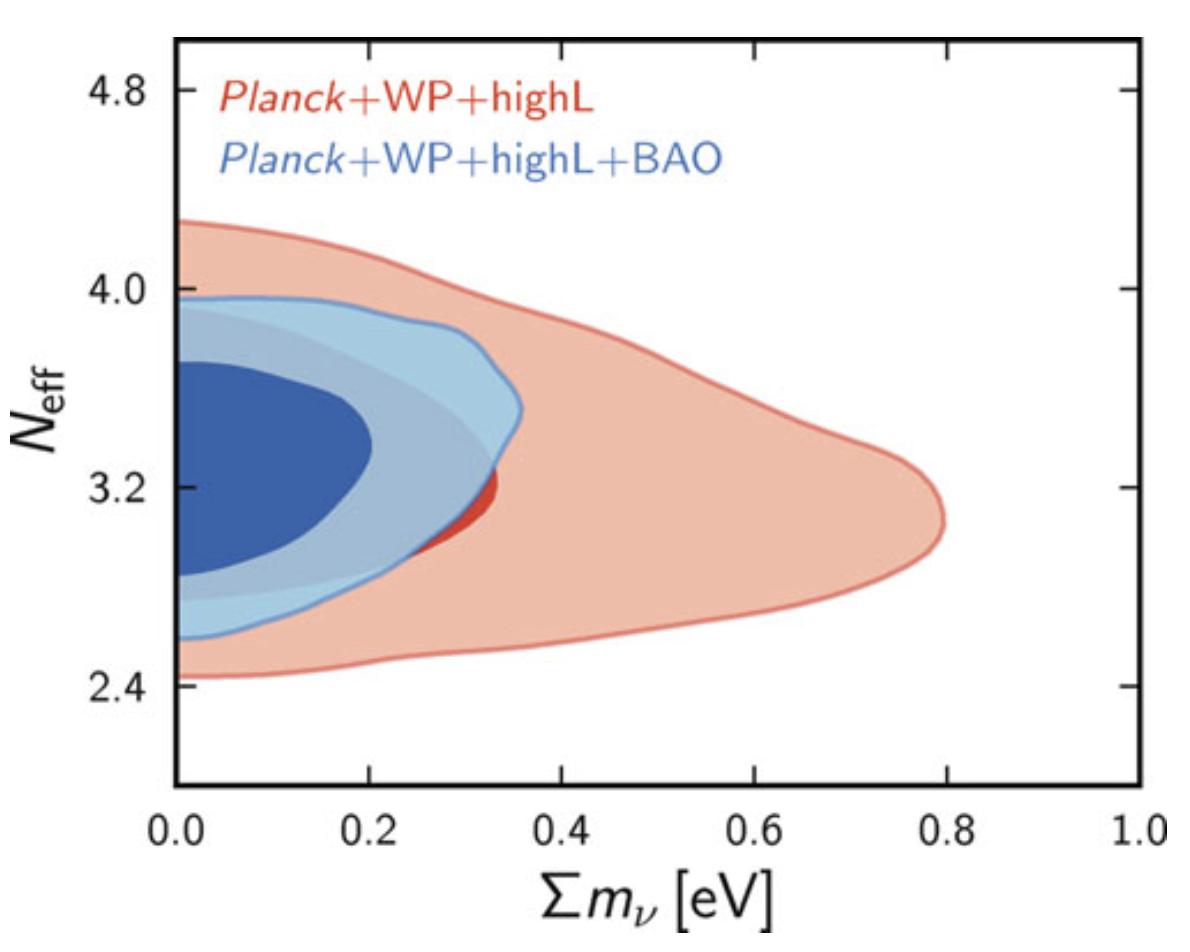
\includegraphics[width=9cm]{figures/cosmology/neutrinomasses.png}}
\end{figure}

{\noindent}In addition to the sun and the CNB, various other astrophysical objects also emit neutrinos. For example, the major fraction of the binding energy released in the formation of compact objects is emitted in the form of neutrinos: about $3\times10^{53}\,{\rm erg}$.

\subsubsection{Follow-up Questions}

\begin{itemize}
    \item What is a neutrino?
    \item How do we determine their mass?
    \item Besides the sun and the CNB, what other sources of neutrinos are there?
    \item What is the neutrino contribution to the density of the Universe?
    \item Why do neutrinos decouple at 1 second (i.e., before photons)?
\end{itemize}


% --------------------------------------------------------------
%
%                           19. 
%
% --------------------------------------------------------------

\newpage
\subsection{Question 19}

What is the difference between an isocurvature mode and an adiabatic mode, in terms of the initial density perturbations in the early Universe? How do we know that the initial conditions are mostly adiabatic?

\subsubsection{Short answer}

An isocurvature mode is one in which density fluctuations of various components balance one another in such a way that there is no net change in the spacetime metric. This is in contrast to adiabatic modes where density fluctuations are proportional to one another which results in a net change of spacetime curvature. 

\subsubsection{Additional context}

In a complete description of energy density perturbations, the total energy density of the Universe includes components of baryonic matter ($\rho_b$), dark matter ($\rho_c$), radiation ($\rho_\mathrm{rad}$), and dark energy ($\rho_\Lambda$):

\begin{align*}
    \rho(\mathbf{x},t) = \rho_b(\mathbf{x},t) + \rho_c(\mathbf{x},t) + \rho_\mathrm{rad}(\mathbf{x},t) + \rho_\Lambda(\mathbf{x},t).
\end{align*}

{\noindent}In terms of their global gravitational influence, dark matter and baryonic matter contribute and evolve equivalently, therefore on cosmological scales they can be combined into a total matter energy density $\rho_m = \rho_b + \rho_c$. Each component may have its own (primordial) perturbation character. Dark energy does not have any density fluctuations, so $\delta_\Lambda(\mathbf{x},t) = 0$. Since most of the structure formation happened during the \textit{matter-dominated era}, this mainly involves the evolution of matter linear perturbations $\delta_m(\mathbf{x},t)$.

{\noindent}Cosmological perturbations will evolve quite differently for different \textbf{perturbation modes}, each of which are identified on the basis of the nature of radiation perturbations with respect to matter perturbations. \textbf{Isothermal perturbation modes} only involve matter perturbations ($\delta_m$) while radiation remains uniformly distributed throughout the 
Universe ($\delta_\mathrm{rad} = 0$). On the other hand, the primordial perturbations $\delta_m$ and $\delta_\mathrm{rad}$ may be completely equivalent (except for a constant proportionality factor) corresponding to zero fluctuations in entropy; these are \textbf{adiabatic perturbation modes}. A third type of perturbation is that of \textbf{isocurvature perturbation modes} in which radiation and matter perturbations cancel each other out such that the local curvature remains equal to the global cosmological curvature. Moreover, the evolution of the various components is complicated to a considerable extent by their mutual interactions. A simple illustration is that of baryonic matter initially without density perturbations: while dark matter creates even deeper potential wells, baryonic matter will fall in and experience increasingly stronger perturbations. Also, in pre-recombination epoch, baryonic matter is closely coupled to radiation such that its evolution is seriously affected by the corresponding radiation pressure gradients.

% --------------------------------------------------------------
%
%                           20. 
%
% --------------------------------------------------------------

\newpage
\subsection{Question 20}

Give three examples of possible dark matter candidates (current or historical). What is their status observationally?

\subsubsection{Short answer}

There is no shortage of candidates for non-baryonic dark matter. The primary candidates include:

\begin{itemize}
    \item WIMPs (weakly interacting massive particles). These are currently purely theoretical and have yet to be detected.
    \item MACHOs (massive compact halo objects). These include white dwarfs, brown dwarfs, black holes etc. These have been detected, of course, but not in large enough quantities to describe the amount of dark matter necessary.
    \item Standard Model neutrinos. These have also been detected but would only work in a HDM cosmology which has already been ruled out in favour of CDM.
\end{itemize}

\subsubsection{Additional context}

{\noindent}There are even more particle candidates...

\begin{itemize}
    \item Sterile neutrinos.
    \item Axions. 
    \item Supersymmetric candidates.
        \item Neutralinos.
        \item Sneutrinos.
        \item Gravitinos.
        \item Axinos.
    \item Light scalar dark matter.
    \item Dark matter from little Higgs models.
    \item Kaluza-Klein states.
    \item Superheavy dark matter.
    \item Q-balls.
\end{itemize}

\subsubsection{Follow-up Questions}

\begin{itemize}
    \item What does the ``hot'' in HDM refer to?
    \item What distinguishes between HDM and CDM?
    \item What is MOND and how does it fit in with DM?
    \item What happens if we don't find WIMPs? How is this search going?
\end{itemize}

% --------------------------------------------------------------
%               Resources 
% --------------------------------------------------------------

\newpage
\subsection{Resources}

\begin{itemize}
    \item Extragalactic Astronomy and Cosmology; Shneider (2006)
    \item Introduction to Cosmology; Ryden (2006)
    \item From First Light to Reionization; Stiavelli (2009)
    \item Modern Cosmology, Dodelson (2003)
    \item 21-cm Cosmology in the 21st Century; Pritchard \& Loelo (2012)
    \item Distance Measures in Cosmology; Hogg (2000)
    \item A CMB Polarization Primer; Hu \& White (1997)
    \item Big Bang Nucleosynthesis; Fields \& Olive (2006)
    \item Cosmic Microwave Background Anisotropies; Hu \& Dodelson (2002)
    \item Lecture Notes on CMB Theory; From Nucleosynthesis to Recombination, Hu (2008)
    \item Observational Probes of Cosmic Acceleration; Weinberg et al. (2013)
    \item Particle Dark Matter: Evidence, Candidates, and Constraints; Bertone et al. (2005)
    \item Observational Constraints on Cosmic Reionization; Fan et al. (2006)
    \item Cosmology with the Sunyaev-Zel'dovich Effect; Carlstrom et al. (2002)
    \item Tired Light and the ``Missing Mass'' Problem; Yourgrau \& Woodward (1971)
    \item On the Robustness of the Acoustic Scale in the Low-Redshift Clustering of Matter; Eisenstein et al. (2007)
    \item Detection of the Baryon Acoustic Peak in the Large-Scale Correlation Function of SDSS Luminous Red Galaxies; Eisenstein et al. (2005)
    \item An Absorption Profile Centered at $78\,{\rm MHz}$ in the Sky-Averaged Spectrum; Bowman et al. (2018)
    \item Can one Measure the Cosmic Neutrino Background; Faessler et al. (2016)
    \item Particle Dark Matter: Evidence, Candidates and Constraints; Bertone et al. (2005)
    \item Cosmology with the Sunyaev-Zeldovich Effect; Carlstrom et al. (2002)
\end{itemize}


































% --------------------------------------------------------------
%
%
%                              EXTRAGALACTIC 
%
%
% --------------------------------------------------------------

\newpage
\section{Extragalactic Astronomy}

% --------------------------------------------------------------
%               1. 
% --------------------------------------------------------------

\subsection{Question 1}

Sketch out the Hubble sequence. What physical trends are captured by the classification system?

\subsubsection{Short answer}

\begin{figure}[h]
    \centering
    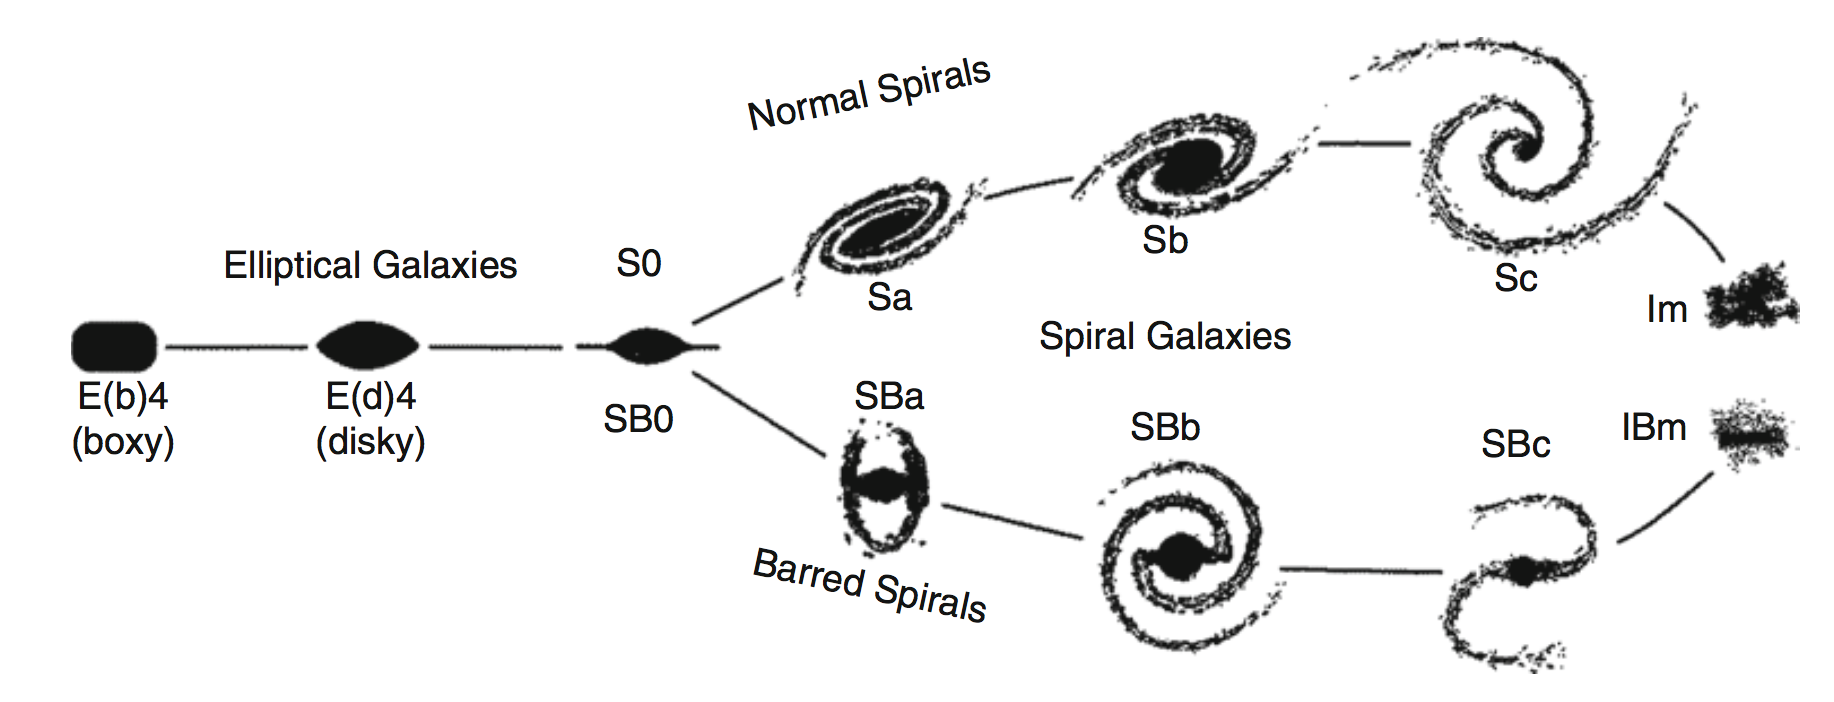
\includegraphics[width=16cm]{figures/extragalactic/HubbleSequence.png}
    \caption{\footnotesize{Hubble’s `tuning fork' for galaxy classification. Adapted from: J. Kormendy \& R. Bender 1996, A Proposed Revision of the Hubble Sequence for Elliptical Galaxies, ApJ 464, L119, Fig. 1. Image taken from Schneider (2006).}}
    \label{fig:hubblesequence}
\end{figure}

\begin{itemize}
    \item Most luminous galaxies in the local Universe fit onto the Hubble sequence; they are either ellipticals, spirals, or belong to the class of S0 galaxies, which shares some properties with the two other classes.
    \item Spiral galaxies consist of a disk with spiral arm structure and a central bulge. They are divided into two subclasses: normal spirals (S's) and barred spirals (SB's).
    \item Elliptical galaxies (E's) are galaxies that have nearly elliptical isophotes without any clearly defined structure.
    \item S0 galaxies are a transition between ellipticals and spirals which are also called lenticulars as they are lentil-shaped galaxies. They contain a bulge and a large enveloping region of relatively unstructured brightness which often appears like a disk without spiral arms.
    \item Irregular galaxies (Irr's) are galaxies with only weak (Irr I) or no (Irr II) regular structure.
    \item Spirals contain a sizable fraction of gas, whereas the gas-to-stellar mass ratio in ellipticals is much smaller. As a consequence, spirals have ongoing star formation, ellipticals not, or only very little. As a further consequence, the light of elliptical galaxies is substantially redder than that of spirals.
    \item The stars in spirals have a very ordered motion, moving around the galactic center on nearly circular orbits in a common orbital plane, having a velocity dispersion that is much smaller than the orbital velocity; the stars in the disk are called `dynamically cold'. In contrast, the motion of stars in ellipticals is largely random, with fairly little coherent velocity; they are `dynamically hot'.
\end{itemize}

\subsubsection{Additional context}

Historically, optical photometry was the method used to observe galaxies. Thus, the morphological classification defined by Hubble is still the best-known today. Besides morphological criteria, color indices, spectroscopic parameters (based on emission or absorption lines), the broad-band spectral distribution (galaxies with/without radio- and/or X-ray emission, or emission in the infrared), as well as other features may also be used.

{\noindent}Figure \ref{fig:hubblesequence} shows the classification scheme defined by Hubble. According to this, three main types of galaxies exist:

\begin{itemize}
    \item \textbf{Elliptical galaxies} (E's) are galaxies that have nearly elliptical isophotes without any clearly defined structure. They are subdivided according to their ellipticity $\epsilon\equiv1-b/a$, where $a$ and $b$ denote the semi-major and the semi-minor axes, respectively. Ellipticals are found over a relatively broad range in ellipticity, $0\leq\epsilon\leq0.7$. The notation E$n$ is commonly used to classify the ellipticals with respect to $\epsilon$, with $n=10\epsilon$; i.e., an E4 galaxy has an axis ratio of $b/a=0.6$, and E0's have circular isophotes.
    \item \textbf{Spiral galaxies} consist of a disk with spiral arm structure and a central bulge. They are divided into two subclasses: normal spirals (S's) and barred spirals (SB's). In each of these subclasses, a sequence is defined that is ordered according to the brightness ratio of bulge and disk, and that is denoted by a, ab, b, bc, c, cd, d. Objects along this sequence are often referred to as being either an early- type or a late-type; hence, an Sa galaxy is an early-type spiral, and an SBc galaxy is a late-type barred spiral. It's stressed explicitly that this nomenclature is not a statement of the evolutionary stage of the objects but is merely a nomenclature of purely historical origin.
    \item \textbf{Irregular galaxies} (Irr's) are galaxies with only weak (Irr I) or no (Irr II) regular structure. The classification of Irr's is often refined. In particular, the sequence of spirals is extended to the classes Sdm, Sm, Im, and Ir (m stands for Magellanic; the Large Magellanic Cloud is of type SBm).
    \item \textbf{S0 galaxies} are a transition between ellipticals and spirals which are also called lenticulars as they are lentil-shaped galaxies. They contain a bulge and a large enveloping region of relatively unstructured brightness which often appears like a disk without spiral arms. Ellipticals and S0 galaxies are referred to as early-type galaxies, spirals as late-type galaxies. As before, these names are only historical and are not meant to describe an evolutionary track!
\end{itemize}

{\noindent}The morphological classification is at least partially affected by projection effects. If, for instance, the spatial shape of an elliptical galaxy is a triaxial ellipsoid, then the observed ellipticity will depend on its orientation with respect to the line-of-sight. Also, it will be difficult to identify a bar in a spiral that is observed from its side (`edge-on').

{\noindent}Besides the aforementioned main types of galaxy morphologies, others exist which do not fit into the Hubble scheme. Many of these are presumably caused by interaction between galaxies. Furthermore, we observe galaxies with radiation characteristics that differ significantly from the spectral behavior of `normal' galaxies.

{\noindent}In summary:

\begin{itemize}
    \item Most luminous galaxies in the local Universe fit onto the Hubble sequence; they are either ellipticals, spirals, or belong to the class of S0 galaxies, which shares some properties with the two other classes.
    \item Ellipticals and spirals differ not only in their morphology, but in several other respects, for example: (1) Spirals contain a sizable fraction of gas, whereas the gas-to- stellar mass ratio in ellipticals is much smaller. As a consequence, (2) spirals have ongoing star formation, ellipticals not, or only very little. As a further consequence, (3) the light of elliptical galaxies is substantially redder than that of spirals. Obviously, the morphology of galaxies and the properties of their stellar populations are strongly correlated.
    \item The stars in spirals have a very ordered motion, moving around the galactic center on nearly circular orbits in a common orbital plane, having a velocity dispersion that is much smaller than the orbital velocity; the stars in the disk are called `dynamically cold'. In contrast, the motion of stars in ellipticals is largely random, with fairly little coherent velocity; they are dynamically hot.
    \item Some elliptical galaxies show clear signs of complex structure, which are interpreted as indications of past interaction with other galaxies. In contrast, the disks of spirals are very thin, which means that they have been largely unperturbed for a long while in the past.
    \item The rotation curves of spiral galaxies are almost flat for large radii, in contrast to what would be expected from the visible mass distribution that declines exponentially outwards. This implies that there is more matter than seen in stars and gas -- the galaxies are embedded in a halo of dark matter. Whereas for elliptical galaxies the radial density distribution is more difficult to probe, the presence of dark matter has been verified also for ellipticals.
    \item Both spirals and ellipticals follow scaling relations which connect their luminous properties (luminosity or surface brightness) with their dynamical properties (rotational velocity or velocity dispersion). Hence, the formation and evolution of galaxies and their stellar populations must proceed in a way as to place them onto these scaling relations.
\end{itemize}

{\noindent}The light from `normal' galaxies is emitted mainly by stars. Therefore, the spectral distribution of the radiation from such galaxies is in principle a superposition of the spectra of their stellar population. The spectrum of stars is, to a first approximation, described by a Planck function that depends only on the star's surface temperature. A typical stellar population covers a temperature range from a few thousand Kelvin up to a few tens of thousand Kelvin. Since the Planck function has a well-localized maximum and from there steeply declines to both sides, most of the energy of such `normal' galaxies is emitted in a relatively narrow frequency interval that is located in the optical and NIR sections of the spectrum.

\begin{figure}[t]
    \centering
    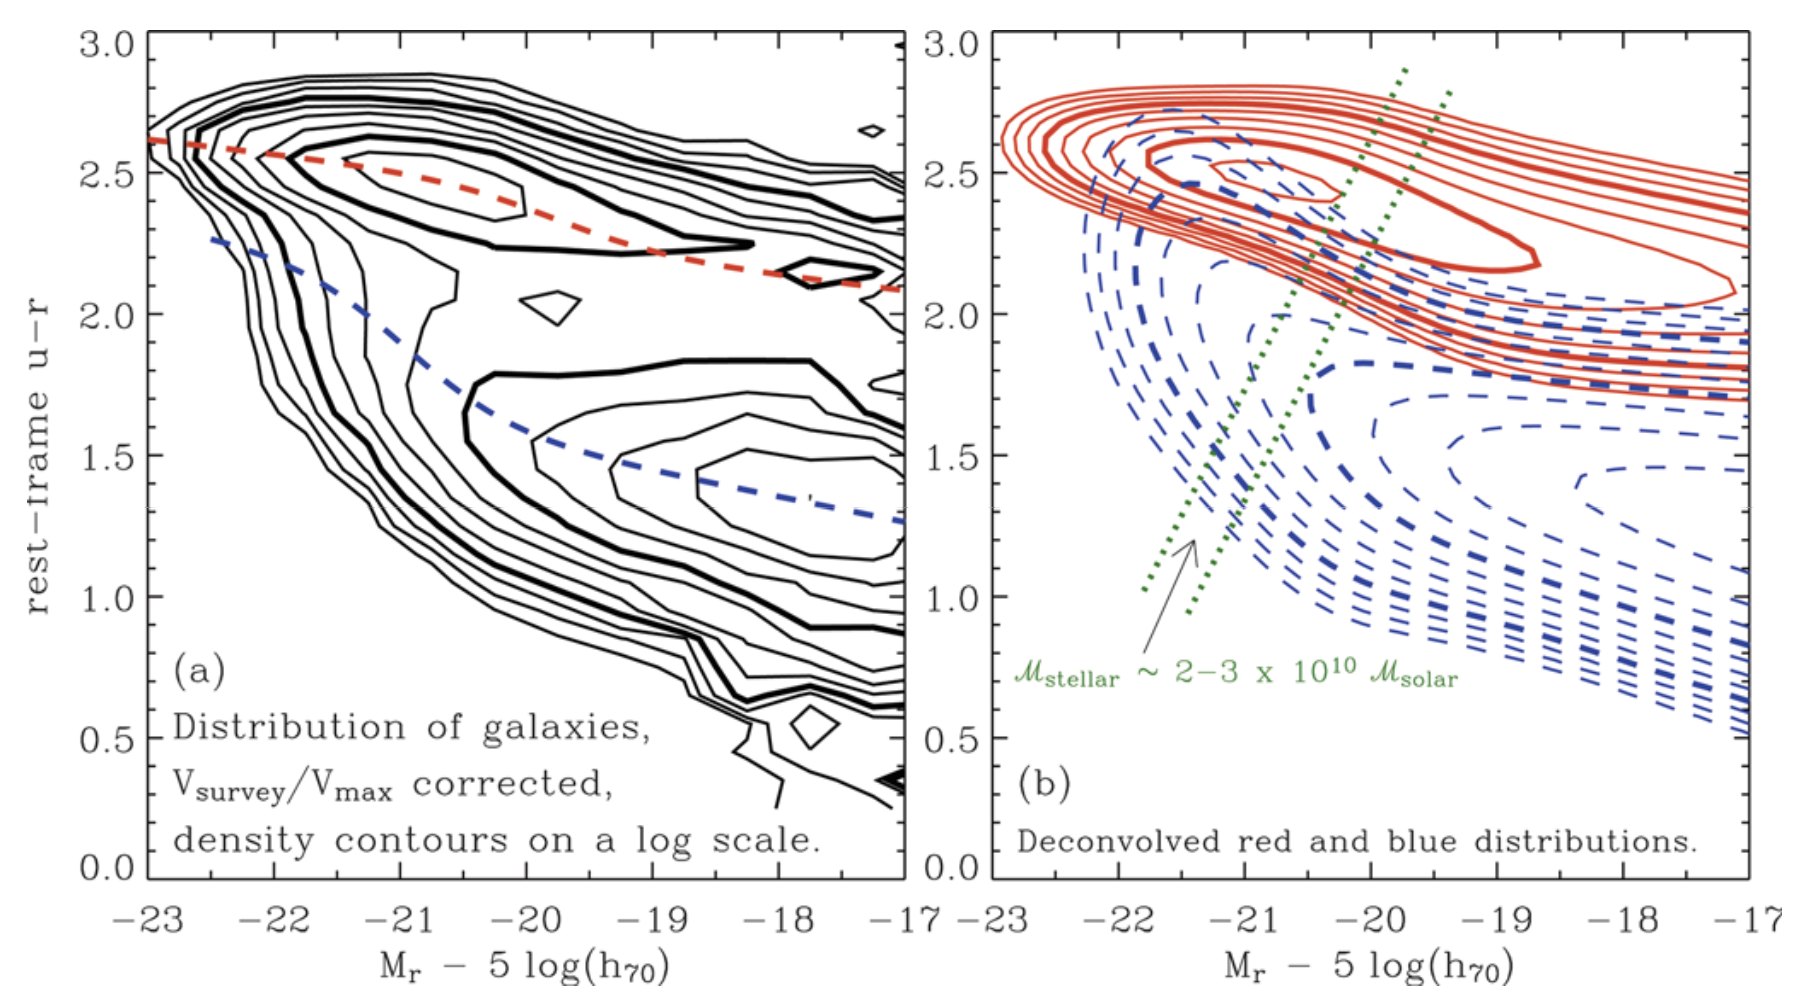
\includegraphics[width=16cm]{figures/extragalactic/SDSSCMD.png}
    \caption{\footnotesize{The density of galaxies in color-magnitude space. The color of $\sim70000$ galaxies with redshifts $0.01\leq z\leq0.08$ from the SDSS is measured by the rest-frame $u-r$, i.e., after a (small) correction for their redshift was applied. The density contours, which were corrected for selection effects, are logarithmically spaced, with a factor of $\sqrt{2}$ between consecutive contours. (a) The measured distribution is shown. Obviously, two peaks of the galaxy density are clearly visible, one at a red color of $u-r\sim2.5$ and an absolute magnitude of $M_r\sim21$,the other at a bluer colour of $u-r\sim1.3$ and significantly fainter magnitudes. (b) Corresponds to the modeled galaxy density. Reused with permission from I.K. Baldry, M.L. Balogh, R. Bower, K. Glazebrook \& R.C. Nichols 2004, Color bimodality: Implications for galaxy evolution, in: THE NEW COSMOLOGY: Conference on Strings and Cosmology, R. Allen (ed.), Conference Proceeding 743, p. 106, Fig. 1 (2004). Figure taken from Schneider (2006).}}
    \label{fig:sdsscmd}
\end{figure}

{\noindent}The classification of galaxies by morphology, given by the Hubble classification scheme (Figure \ref{fig:hubblesequence}), has the disadvantage that morphologies of galaxies are not easy to quantify. Traditionally, this was done by visual inspection but of course this method bears some subjectivity of the researcher doing it and requires a lot of experience. Furthermore, this visual inspection is time consuming and cannot be performed on large samples of galaxies. Various techniques and related software were developed to perform such a classification automatically, in many cases with significant success, including the reproducibility of galaxy classification between different methods. Nevertheless, quite a number of problems remain, such as the inclination dependence of the morphological appearance of a galaxy.

{\noindent}Even automatic classifications cannot be applied to galaxies for which the angular resolution of the imaging is not much better than the angular size of galaxies, that is, for distant objects. An alternative to morphological classification is provided by the colours of galaxies, which can be obtained from broad-band multi-color imaging. Colors are much easier to measure than morphology, in particular for very small galaxies. In addition, the physical properties of galaxies may be better characterized by their colors than by their morphology -- the colours yield information about the stellar population, whereas the morphology is determined by the dynamics of the galaxy.

{\noindent}Using photometric measurements and spectroscopy from the SDSS, the colours and absolute magnitudes of low-redshift galaxies have been studied; their density distribution in a color-magnitude diagram is plotted in the left-hand side of Figure \ref{fig:sdsscmd}. We see immediately that there are two density peaks of the galaxy distribution in this diagram: one at high luminosities and red color, the other at significantly fainter absolute magnitudes and much bluer color. It appears that the galaxies are distributed at and around these two density peaks, hence galaxies tend to be either luminous and red, or less luminous and blue. We can also easily see from this diagram that the distribution of red and blue galaxies with respect to their luminosity is different, the former one being more shifted towards larger luminosity.

{\noindent}We can next consider the color distribution of galaxies at a fixed absolute magnitude $M_r$. This is obtained by plotting the galaxy number density along vertical cuts through the left-hand side of Figure \ref{fig:sdsscmd}. When this is done for different $M_r$, it turns out that the colour distribution of galaxies is bimodal: over a broad range in absolute magnitude, the color distribution has two peaks, one at red, the other at blue $u-r$. Again, this fact can be seen directly from Figure \ref{fig:sdsscmd}. For each value of $M_r$, the colour distribution of galaxies can be very well fitted by the sum of two Gaussian functions. The central colors of the two Gaussians are shown by the two dashed curves in the left panel of Figure \ref{fig:sdsscmd}. They become redder the more luminous the galaxies are. This luminosity-dependent reddening is considerably more pronounced for the blue population than for the red galaxies.

{\noindent}To see how good this fit indeed is, the right-hand side of Figure \ref{fig:sdsscmd} shows the galaxy density as obtained from the two-Gaussian fits, with solid contours corresponding to the red galaxies and dashed contours to the blue ones. We thus conclude that the local galaxy population can be described as a bimodal distribution in $u-r$ color, where the characteristic color depends slightly on absolute magnitude. The galaxy distribution at bright absolute magnitudes is dominated by red galaxies, whereas for less luminous galaxies the blue population dominates.

{\noindent}The mass-to-light ratio of a red stellar population is larger than that of a blue population, since the former no longer contains massive luminous stars. The difference in the peak absolute magnitude between the red and blue galaxies therefore corresponds to an even larger difference in the stellar mass of these two populations. Red galaxies in the local Universe have on average a much higher stellar mass than blue galaxies. This fact is illustrated by the two dotted lines in the right-hand panel of Figure \ref{fig:sdsscmd} which correspond to lines of constant stellar mass of $\sim2-3\times10^{10}\,{\rm M}$. This seems to indicate a very characteristic mass scale for the galaxy distribution: most galaxies with a stellar mass larger than this characteristic mass scale are red, whereas most of those with a lower stellar mass are blue.

\begin{table}[t]
    \centering
    \includegraphics[width=16cm]{figures/extragalactic/LateGalaxies.png}
    \caption{\footnotesize{Characteristic values for late-type (i.e., spiral) galaxies. $V_\mathrm{max}$ is the maximum rotation velocity, thus characterizing the flat part of the rotation curve. The opening angle is the angle under which the spiral arms branch off, i.e., the angle between the tangent to the spiral arms and the circle around the center of the galaxy running through this tangential point. $S_N$ is the specific abundance of globular clusters. The values in this table are taken from the book by Carroll \& Ostlie. Table taken from Schneider (2006).}}
    \label{table:lategalaxies}
\end{table}

{\noindent}Looking at the sequence of early-type spirals (i.e., Sa's or SBa's) to late-type spirals, we find a number of differences that can be used for classification:

\begin{itemize}
    \item A decreasing luminosity ratio of bulge and disk, with $L_\mathrm{bulge}/L_\mathrm{disk}\sim0.3$ for Sa’s and $\sim0.05$ for Sc’s
    \item An increasing opening angle of the spiral arms, from   $6^\circ$ for Sa's to $18^\circ$ for Sc's.
    \item An increasing brightness structure along the spiral arms: Sa's have a `smooth' distribution of stars along the spiral arms, whereas the light distribution in the spiral arms of Sc's is resolved into bright knots of stars and HII regions.
\end{itemize}

{\noindent}Bars are common in spiral galaxies, with $\sim70\%$ of all disk galaxies containing a large-scale stellar bar. Such a bar perturbs the axial symmetry of the gravitational potential in a galaxy, which may have a number of consequences. One of them is that this perturbation can lead to a redistribution of angular momentum of the stars, gas, and dark matter. In addition, by perturbing the orbits, gas can be driven towards the center of the galaxy which may have important consequences for triggering nuclear activity and enhanced star formation.

{\noindent}The light profile of the bulge of spirals is described by a \textbf{de Vaucouleurs profile} to a first approximation, while the disk follows an exponential brightness profile, as is the case for our MW. Expressing these distributions of the surface brightness in $\mu\propto-2.5\log(I)$, measured in ${\rm mag\,arcsec^{-2}}$, we obtain

\begin{align*}
    \mu_\mathrm{bulge} = \mu_e + 8.3268\left[\left(\frac{R}{R_e}\right)^{1/4}-1\right] ~ [{\rm mag\,arcsec^{-2}}]
\end{align*}

{\noindent}and

\begin{align*}
    \mu_\mathrm{disk} = \mu_0 + 1.09\left(\frac{R}{h_R}\right) ~ [{\rm mag\,arcsec^{-2}}].
\end{align*}

{\noindent}Here, $\mu_e$ is the surface brightness at the effective radius $R_e$ which is defined such that half of the bulge luminosity is emitted within $R_e$. The central surface brightness and the scale-length of the disk are denoted by $\mu_0$ and $h_R$, respectively. It has to be noted that $\mu_0$ is not directly measurable since $\mu_0$ is not the central surface brightness of the galaxy, only that of its disk component. To determine $\mu_0$, the exponential law is extrapolated from large $R$ inwards to $R=0$, or more precisely, by fitting the sum of an exponential and a bulge component to the total light profile of the galaxy.

{\noindent}The brightness profile of spiral disks perpendicular to the disk can be studied exclusively in edge-on spirals. From them, one finds that it is in general well described by an exponential law. The scale-height $h_z$ of the disk is almost independent of the galacto-centric radius $R$, and between galaxies scales roughly linearly with the rotational velocity of the disk. The typical value for the ratio of scale-height to scale-length is $h_z/h_R=0.07$ -- indeed, the disks of spiral galaxies are thin. The flattest galaxies are those of late Hubble type.

{\noindent}While the brightness profile of bulges follows approximately that of a de Vaucouleurs profile, some spiral galaxies bulges were found which behave differently than these `classical' bulges; one calls them \textbf{pseudobulges}. In contrast to classical bulges, they follow more an exponential profile, are typically flatter, and have significant rotational support. Furthermore, whereas classical bulges lie on the same sequence in the effective radius vs. absolute magnitude diagram as the ellipticals, pseudobulges do not. They have lower luminosity for a given size.

{\noindent}In many cases it is very difficult to distinguish between both types of bulges photometrically. However, spectroscopy aids a lot in this distinction. In fact, some bulges of spirals have two components, i.e., both a classical bulge and a pseudobulge.

{\noindent}The differences in the two types of bulges suggest that they should have a different origin. Classical bulges behave like a small elliptical galaxy. It is believed that ellipticals form through merging events of galaxies which `heats up' the stellar velocity distribution (i.e., turns ordered velocity fields of disk galaxies into random orbits which are characteristic for ellipticals). Therefore, in the current model of galaxy evolution, classical bulges are also formed as a result of merger events. In contrast, the ordered rotation of pseudobulges suggests that they have evolved from the disk population. For example, symmetry perturbations of the gravitational field caused by a bar can generate random velocity components of stars perpendicular to the plane of the disk, and thus thicken the disk population in the inner part of a galaxy.

{\noindent}Whereas pseudobulges may provide important insights into the evolution of galaxies, they are a sub-dominant component in the population of galaxies. It is estimated that classical bulges together contain about ten times more stars than pseudobulges. Therefore, whenever the term `bulge' is used, it's often implicitly meant to refer to the classical bulges.

{\noindent}Some late-type spiral galaxies seem to have no bulge component. Some of them show instead a nuclear stellar cluster at their center. These nuclear star clusters appear at first sight to be similar to globular clusters. However, their stellar population is quite different from that of the old globular clusters in our Galaxy, as their light is dominated by a relatively young stellar population, although their stellar mass is totally dominated by an old population. In some respect, these nuclear star clusters share properties with the peculiar Galactic globular $\omega$ Centauri, which also shows a broad range of stellar ages and an inhomogeneous chemical abundance. Therefore, it has been hypothesized that $\omega$ Centaurus is the remnant of a merger of a lower mass galaxy with the MW.

{\noindent}The general term `elliptical galaxies' (or ellipticals, for short) covers a broad class of galaxies which differ in their luminosities and sizes. A rough subdivision is as follows:

\begin{itemize}
    \item \textbf{Normal ellipticals}: This class includes giant ellipticals (gE's), those of intermediate luminosity (E's), and compact ellipticals (cE's), covering a range in absolute magnitudes from $M_B\sim23$ to $M_B\sim15$.
    \item \textbf{Dwarf ellipticals (dE's)}: These differ from the cE's in that they have a significantly smaller surface brightness and a lower metallicity.
    \item \textbf{cD galaxies}: These are extremely luminous (up to $M_B\sim25$) and large (up to $R\sim1{\rm Mpc}$) galaxies that are only found near the centers of dense clusters of galaxies. Their surface brightness is very high close to the center, they have an extended diffuse envelope, and they have a very high $M/L$ ratio. It is not clear whether the extended envelope actually `belongs' to the galaxy or is part of the galaxy cluster in which the cD is embedded, since such clusters are now known to have a population of stars located outside of the cluster galaxies.
    \item \textbf{Blue compact dwarf galaxies}: These `blue compact dwarfs' (BCD’s) are clearly bluer (with $(B-V)$ between $0.0$ and $0.3$) than the other ellipticals, and contain an appreciable amount of gas in comparison.
    \item \textbf{Dwarf spheroidals (dSph's)}: These exhibit a very low luminosity and surface brightness. They have been observed down to $M_B\sim8$. Due to these properties, they have thus far only been observed in the Local Group.
\end{itemize}

\begin{table}[t]
    \centering
    \includegraphics[width=16cm]{figures/extragalactic/EarlyGalaxies.png}
    \caption{\footnotesize{Characteristic values for early-type galaxies. $D_{25}$ denotes the diameter at which the surface brightness has decreased to $25\,{\rm B-mag\,arcsec^{-2}}$ , $S_N$ is the `specific frequency', a measure for the number of globular clusters in relation to the visual luminosity, and $M/L$ is the mass-to-light ratio in Solar units. The values of this table are taken from the book by Carroll \& Ostlie. Table taken from Schneider (2006).}}
    \label{table:earlygalaxies}
\end{table}

{\noindent}Analyzing the morphology of elliptical galaxies raises a simple question: Why are ellipticals not round? A simple explanation would be rotational flattening, i.e., as in a rotating self-gravitating gas ball, the stellar distribution bulges outwards at the equator due to centrifugal forces, as is also the case for the Earth. If this explanation was correct, the rotational velocity $v_\mathrm{rot}$, which is measurable in the relative Doppler shift of absorption lines, would have to be of about the same magnitude as the velocity dispersion of the stars $\sigma_v$ that is measurable through the Doppler broadening of lines. More precisely, by means of stellar dynamics one can show that for the rotational flattening of an axially symmetric, oblate galaxy, the relation

\begin{align*}
    \left(\frac{v_\mathrm{rot}}{\sigma_v}\right)_\mathrm{iso} = \sqrt{\frac{\epsilon}{1-\epsilon}} ~ [{\rm dimensionless}]
\end{align*}

{\noindent}has to be satisfied, where `iso' indicates the assumption of an isotropic velocity distribution of the stars. However, for very luminous ellipticals one finds that, in general, $v_\mathrm{rot}\ll \sigma_v$, so that rotation cannot be the major cause of their ellipticity. In addition, many ellipticals are presumably triaxial, so that no unambiguous rotation axis is defined. Thus, luminous ellipticals are in general not rotationally flattened. For less luminous ellipticals and for the bulges of disk galaxies, however, rotational flattening can play an important role. The question remains of how to explain a stable elliptical distribution of stars without bulk rotation.

{\noindent}The brightness profile of an elliptical galaxy is defined by the distribution of its stellar orbits. Let us assume that the gravitational potential is given. The stars are then placed into this potential, with the initial positions and velocities following a specified distribution. If this distribution is not isotropic in velocity space, the resulting light distribution will in general not be spherical. For instance, one could imagine that the orbital planes of the stars have a preferred direction, but that an equal number of stars exists with positive and negative angular momentum $L_z$, so that the total stellar distribution has no net angular momentum and therefore does not rotate. Each star moves along its orbit in the gravitational potential, where the orbits are in general not closed. If an initial distribution of stellar orbits is chosen such that the statistical properties of the distribution of the orbits are invariant in time, then one will obtain a stationary system. If, in addition, the distribution is chosen such that the respective mass distribution of the stars will generate exactly the originally chosen gravitational potential, one arrives at a self-gravitating equilibrium system. In general, it is a difficult mathematical problem to construct such self-gravitating equilibrium systems. Furthermore, elliptical galaxies also contain a dark matter component, whose gravitational potential adds to that of the stars.

{\noindent}The question now arises whether such an equilibrium system can also be stable in time. One might expect that close encounters of pairs of stars would cause a noticeable disturbance in the distribution of orbits. These pair-wise collisions could then lead to a `thermalization' of the stellar orbits. To examine this question we need to estimate the time-scale for such collisions and the changes in direction they cause.

{\noindent}For this purpose, we consider the relaxation time-scale by pair collisions in a system of $N$ stars of mass $m$, total mass $M=Nm$, extent $R$, and a mean stellar density of $n=3N/(4\pi R^3)$. We define the relaxation time $t_\mathrm{relax}$ as the characteristic time in which a star changes its velocity direction by $\sim90^\circ$ due to pair collisions with other stars. By simple calculation (see below), we find that

\begin{align*}
    t_\mathrm{relax} \approx \frac{R}{6v} \frac{N}{\ln(N/2)} ~ [{\rm yr}]
\end{align*}

{\noindent}or

\begin{align*}
    t_\mathrm{relax} = \frac{t_\mathrm{cross}}{6} \frac{N}{\ln(N/2)} ~ [{\rm yr}],
\end{align*}

{\noindent}where $t_\mathrm{cross}=R/v$ is the crossing time-scale, i.e. the time it takes a star to cross the stellar system. If we now consider a typical galaxy, with $t_\mathrm{cross}\sim10^8\,{\rm yr}$, $N\sim10^{12}$ (thus $ln(N/2)\sim30$), then we find that the relaxation time is much longer than the age of the Universe. This means that pair collisions do not play any role in the evolution of stellar orbits. The dynamics of the orbits are determined solely by the large-scale gravitational field of the galaxy. There is a process called violent relaxation which most likely plays a central role in the formation of galaxies and which is probably also responsible for the stellar orbits establishing an equilibrium configuration.

{\noindent}We thus conclude that the stars behave like a collisionless gas: elliptical galaxies are stabilized by (dynamical) pressure, and they are elliptical because the stellar distribution is anisotropic in velocity space. This corresponds to an anisotropic pressure -- where we recall that the pressure of a gas is nothing but the momentum transport of gas particles due to their thermal motion.


\subsubsection{Follow-up Questions}

\begin{itemize}
    \item What physical trends does the Hubble sequence show that were not explicitly encoded in it? (i.e., spiral arm tightness and bulge size are properties that Hubble based the sequence off of.)
    \item Are there any other physical properties that the Hubble sequence ended up telling us about (i.e., by `accident')?
    \item Do most observable galaxies fall somewhere on the Hubble sequence?
    \item Describe how galaxies form and evolve.
\end{itemize}


% --------------------------------------------------------------
%               2. 
% --------------------------------------------------------------

\newpage
\subsection{Question 2}

What is the total mass (in both dark matter and in stars) of the Milky Way galaxy? How does this compare to M31 and to the LMC? How is this mass determined?

\subsubsection{Short answer}

The MWG has a total mass of about $10^{12}\,{\rm M_\odot}$. This is about the same as M31 (Andromeda), and larger than the LMC which is roughly $10^{10}\,{\rm M_\odot}$. Assuming virial equlibrium, the mass can be determined from the flat part of the rotation curve via

\begin{align*}
    V_0 = \sqrt{\frac{GM(<R)}{R_0}} ~ [{\rm m\,s^{-1}}].
\end{align*}

{\noindent}If spiral galaxies are being observed, the Tully-Fisher relation $L\propto v_\mathrm{max}^4$ can be used to determine the maximum orbital velocity in replacement of the rotation curve. Similarly, if elliptical galaxies are being observed, the Faber-Jackson relation $L\propto\sigma_v^4$ can be used instead.

\subsubsection{Additional context}

The components of the Milky Way Galaxy (MWG) have total masses as follows: a disk mass of $4.5\times10^{10}\,{\rm M_\odot}$, bulge mass of $4.5\times10^9\,{\rm M_\odot}$, dark halo mass of $2\times10^{12}\,{\rm M_\odot}$, and BH mass of $4\times10^6\,{\rm M_\odot}$.

{\noindent}The Galactic disk rotates, with rotational velocity $V(R)$ depending on the distance $R$ from the center. We can estimate the mass of the Galaxy from the distribution of the stellar light and the mean mass-to-light ratio of the stellar population, since gas and dust represent less than $\sim10$\% of the mass of the stars. From this mass estimate we can predict the rotational velocity as a function of radius simply from Newtonian mechanics. However, the observed rotational velocity of the Sun around the Galactic center is significantly higher than would be expected from the observed mass distribution. If $M(<R_0)$ is the mass inside a sphere around the Galactic center with radius $R_0=8\,{\rm kpc}$, then the rotational velocity from Newtonian mechanics is

\begin{align*}
    V_0 = \sqrt{\frac{GM(<R)}{R_0}} ~ [{\rm m\,s^{-1}}].
\end{align*}

{\noindent}From the visible matter in stars we would expect a rotational velocity of $160\,{\rm km\,s}$, but we observe $V_0=220\,{\rm km\,s}$ (see Figure \ref{fig:rotationcurve}). This discrepancy, and the shape of the rotation curve $V(R)$ for larger distances $R$ from the Galactic center, indicates that our Galaxy contains significantly more mass than is visible in the form of stars. This additional mass is called dark matter. Its physical nature is still unknown. The main candidates are weakly interacting elementary particles like those postulated by some elementary particle theories, but they have yet not been detected in the laboratory. Macroscopic objects (i.e., celestial bodies) are also in principle viable candidates if they emit very little light.

\begin{figure}[h]
    \floatbox[{\capbeside\thisfloatsetup{capbesideposition={right,top},capbesidewidth=4cm}}]{figure}[\FBwidth]
    {\caption{\footnotesize{The upper curve is the observed rotation curve $V(R)$ of our Galaxy, i.e., the rotational velocity of stars and gas around the Galactic center as a function of their galacto-centric distance. The lower curve is the rotation curve that we would predict based solely on the observed stellar mass of the Galaxy. The difference between these two curves is ascribed to the presence of dark matter, in which the Milky Way disk is embedded. This image is adapted from Nick Strobel's webpage at \href{www.astronomynotes.com}{www.astronomynotes.com}. Image taken from Schneider (2006).}}
    \label{fig:rotationcurve}}
    {\includegraphics[width=10cm]{figures/extragalactic/RotationCurve.png}}
\end{figure}

\newpage
\subsubsection{Follow-up Questions}

\begin{itemize}
    \item If rotation curve/lensing measurements were instead due to modified gravity, how could we tell?
    \item What are $\Omega_m$ and $\Omega_b$ estimated to be? Why does the ratio of the two differ from the star/total mass ratio you have here? Where is all the extra baryonic mass?
    \item When you say we estimate stellar mass by ``counting stars'', what does that mean?
\end{itemize}

% --------------------------------------------------------------
%               3. 
% --------------------------------------------------------------

\newpage
\subsection{Question 3}

Describe as many steps of the distance ladder and the involved techniques as you can. What are the rough distances to the Magellanic Clouds, Andromeda, and the Virgo Cluster?

\subsubsection{Short answer}

The rough distances to the Magellanic Clouds, Andromeda, and the Virgo Cluster are as follows:

\begin{align*}
    d_\mathrm{LMC} \approx 50 ~ [{\rm kpc}] \\
    d_\mathrm{SMC} \approx 60 ~ [{\rm kpc}] \\
    d_\mathrm{M31} \approx 700 ~ [{\rm kpc}] \\
    d_\mathrm{Virgo} \approx 10 ~ [{\rm Mpc}].
\end{align*}

\subsubsection{Additional context}

{\noindent}\textbf{Trigonometric parallax ($<30\,{\rm pc}$)}: The most important method of distance determination is the trigonometric parallax, not only from a historical point-of-view. This method is based on a purely geometric effect and is therefore independent of any physical assumptions. Due to the motion of the Earth around the Sun the positions of nearby stars on the sphere change relative to those of very distant sources (e.g., extragalactic objects such as quasars). The latter therefore define a fixed reference frame on the sphere. In the course of a year the apparent position of a nearby star follows an ellipse on the sphere, the semi-major axis of which is called the parallax. The axis ratio of this ellipse depends on the direction of the star relative to the ecliptic (the plane that is defined by the orbits of the Earth and the other planets). The parallax depends on the radius $r$ of the Earth’s orbit, hence on the Earth-Sun distance which is, by definition, one astronomical unit (AU). Furthermore, the parallax depends on the distance $d$ of the star,

\begin{align*}
    \frac{r}{d} = \tan(p) \approx p ~ [{\rm rad}].
\end{align*}

{\noindent}where we used $p\ll1$ in the last step, and $p$ is measured in radians as usual. The trigonometric parallax is also used to define the common unit of distance in astronomy: one parsec (pc) is the distance of a hypothetical source for which the parallax is exactly $p=1''$. With the conversion of arcseconds to radians ($1''\approx4.848\times10^{-6}\,{\rm rad}$) one gets $p/1''=206265p$, which for a parsec yields

\begin{align*}
    1\,{\rm pc} = 206265\,{\rm AU} = 3.086\times10^{16}\,{\rm m}.
\end{align*}

{\noindent}The distance corresponding to a measured parallax is then
calculated as

\begin{align*}
    d = \left(\frac{p}{1''}\right)^{-1}\,{[\rm pc]}.
\end{align*}

{\noindent}o determine the parallax p, precise measurements of the position of an object at different times are needed, spread over a year, allowing us to measure the ellipse drawn on the sphere by the object’s apparent position. For ground-based observations the accuracy of this method is limited by the atmosphere. The seeing causes a blurring of the images of astronomical sources and thus limits the accuracy of position measurements. From the ground this method is therefore limited to parallaxes larger than $\approx0.1''$, implying that the trigonometric parallax yields distances to stars only within $\approx30\,{\rm pc}$.

{\noindent}\textbf{Proper motions}: Stars are moving relative to us or, more precisely, relative to the Sun. To study the kinematics of the Milky Way we need to be able to measure the velocities of stars. The radial component $v_r$ of the velocity is easily obtained from the Doppler shift of spectral lines,

\begin{align*}
    v_r = \left(\frac{\Delta\lambda}{\lambda_0}\right)c ~ [{\rm m\,s^{-1}}]
\end{align*}

{\noindent}where $\lambda_)$ is the rest-frame wavelength of an atomic transition and $\Delta\lambda=\lambda-\lambda_0$ is the Doppler shift of the wavelength due to the radial velocity of the source. The sign of the radial velocity is defined such that $v_r>0$ corresponds to a motion away from us, i.e., to a redshift of spectral lines.

{\noindent}In contrast, the determination of the other two velocity components is much more difficult. The tangential component, $v_t$, of the velocity can be obtained from the proper motion of an object. In addition to the motion caused by the parallax, stars also change their positions on the sphere as a function of time because of the transverse component of their velocity relative to the Sun. The proper motion $\mu$ is thus an angular velocity, e.g., measured in milliarcseconds per year (mas/yr or $''/{\rm year}$). This angular velocity is linked to the tangential velocity component via

\begin{align*}
    v_t = d\mu = 4.74\left(\frac{d}{1\,{\rm pc}}\right) \left(\frac{\mu}{1''\,{\rm year^{-1}}}\right) ~ [{\rm m\,s^{-1}}].
\end{align*}

{\noindent}Therefore, one can calculate the tangential velocity from the proper motion and the distance. If the latter is derived from the trigonometric parallax, these can be combined to yield

\begin{align*}
    v_t = d\mu = 4.74 \left(\frac{\mu}{1\,''\,{\rm year^{-1}}}\right) \left(\frac{p}{1''}\right)^{-1} ~ [{\rm m\,s^{-1}}].
\end{align*}

{\noindent}Of course, the proper motion has two components, corresponding to the absolute value of the angular velocity and its direction on the sphere. Together with $v_r$ this determines the three-dimensional velocity vector. Correcting for the known velocity of the Earth around the Sun, one can then compute the velocity vector v of the star relative to the Sun, called the heliocentric velocity.

{\noindent}\textbf{Moving cluster parallax ($<200\,{\rm pc}$)}: The stars in an (open) star cluster all have a very similar spatial velocity. This implies that their proper motion vectors should be similar. To what accuracy the proper motions are aligned depends on the angular extent of the star cluster on the sphere. Like two railway tracks that run parallel but do not appear parallel to us, the vectors of proper motions in a star cluster also do not appear parallel. They are directed towards a convergence point, as depicted in Figure \ref{fig:clusterparallax}.

\begin{figure}[h]
    \floatbox[{\capbeside\thisfloatsetup{capbesideposition={right,top},capbesidewidth=4cm}}]{figure}[\FBwidth]
    {\caption{\footnotesize{The moving cluster parallax is a projection effect, similar to that known from viewing railway tracks. The directions of velocity vectors pointing away from us seem to converge and intersect at the convergence point. The connecting line from the observer to the convergence point is parallel to the velocity vector of the star cluster. Image taken from Schneider (2006).}}
    \label{fig:clusterparallax}}
    {\includegraphics[width=10cm]{figures/extragalactic/ClusterParallax.png}}
\end{figure}

{\noindent}We consider a star cluster and assume that all stars have the same spatial velocity $v$. The position of the i-th star as a function of time is then described by

\begin{align*}
    \mathbf{r}_i(t) = \mathbf{r}_i(t) + \mathbf{v}t ~ [{\rm m}],
\end{align*}

{\noindent}where $\mathbf{r}_i$ is the current position if we identify the origin of time, $t=0$, with `today'. The direction of a star relative to us is described by the unit vector

\begin{align*}
    \mathbf{n}_i(t) \equiv \frac{\mathbf{r}_i}{\lvert\mathbf{r}_i\rvert} ~ [{\rm dimensionless}].
\end{align*}

{\noindent}From this, one infers that for large times, $t\rightarrow\infty$, the direction vectors of the convergence point are identical for all stars in the cluster,

\begin{align*}
    \mathbf{n}_i(t) \rightarrow \frac{\mathbf{v}}{\lvert\mathbf{v}\rvert} \equiv \mathbf{n}_\mathrm{conv} ~ [{\rm dimensionless}].
\end{align*}

{\noindent}Hence for large times all stars will appear at the same point $\mathbf{n}_\mathrm{conv}$: the convergence point. This only depends on the direction of the velocity vector of the star cluster. In other words, the direction vector of the stars is such that they are all moving towards the convergence point. Thus, $\mathbf{n}_\mathrm{conv}$ (and hence $\mathbf{v}/\lvert\mathbf{v}\rvert$) can be measured from the direction of the proper motions of the stars in the cluster. On the other hand, one component of $\mathbf{v}$ can be determined from the (easily measured) radial velocity $\mathbf{v}_r$. With these two observables the three-dimensional velocity vector $\mathbf{v}$ is completely determined, as is easily demonstrated: let $\theta$ be the angle between the line-of-sight $\mathbf{n}$ towards a star in the cluster and $\mathbf{v}$. The angle is directly read off from the direction vector $\mathbf{n}$ and the convergence point, $\cos\theta = \mathbf{n}\cdot\mathbf{v}/\lvert\mathbf{v}\rvert = \mathbf{}_\mathrm{conv}\cdot\mathbf{n}$. With $v\equiv\lvert\mathbf{v}\rvert$ one then obtains

\begin{align*}
    v_r = v\cos\theta ~ [{\rm m\,s^{-1}}], ~~~~~ v_t = v\sin\theta ~ [{\rm m\,s^{-1}}],
\end{align*}

{\noindent}and so

\begin{align*}
    v_t = v_r\tan\theta ~ [{\rm m\,s^{-1}}].
\end{align*}

{\noindent}This means that the tangential velocity $\mathbf{v}_t$ can be measured without determining the distance to the stars in the cluster. On the other hand, we have a relation between the proper motion, the distance, and $\mathbf{v}$. Hence, a distance determination for the star is now possible with

\begin{align*}
    \mu = \frac{v_t}{d} = \frac{v_r\tan\theta}{d} \rightarrow d = \frac{v_r\tan\theta}{\mu} ~ [{\rm pc}].
\end{align*}

{\noindent}This method yields accurate distance estimates of star clusters within $\sim200\,{\rm pc}$. The accuracy depends on the measurability of the proper motions. Furthermore, the cluster should cover a sufficiently large area on the sky for the convergence point to be well defined. For the distance estimate, one can then take the average over a large number of stars in the cluster if one assumes that the spatial extent of the cluster is much smaller than its distance to us.

{\noindent}\textbf{Main sequence fitting}: Most stars in the color-magnitude diagram (CMD) are located along the main sequence. This enables us to compile a calibrated main sequence of those stars whose trigonometric parallaxes are measured, thus with known distances. Utilizing photo- metric methods, it is then possible to derive the distance to a star cluster. 

{\noindent}The stars of a star cluster define their own main sequence; since they are all located at the same distance, their main sequence is already defined in a CMD in which only apparent magnitudes are plotted. This cluster main sequence can then be fitted to a calibrated main sequence by a suitable choice of the distance, i.e., by adjusting the \textbf{distance modulus} $m-M$,

\begin{align*}
    m-M = 5\log(d/{\rm pc}) - 5 ~ [{\rm mag}],
\end{align*}

{\noindent}where $m$ and $M$ denote the apparent and absolute magnitude, respectively.

{\noindent}In reality this method cannot be applied so easily since the position of a star on the main sequence does not only depend on its mass but also on its age and metallicity. Furthermore, only stars of luminosity class V (i.e., dwarf stars) define the main sequence, but without spectroscopic data it is not possible to determine the luminosity class.

{\noindent}\textbf{Extinction and reddening}: Another major problem is extinction. Absorption and scattering of light by dust affect the relation of absolute to apparent magnitude: for a given $M$, the apparent magnitude $m$ becomes larger (fainter) in the case of absorption, making the source appear dimmer. Also, since extinction depends on wavelength, the spectral energy distribution of the source is modified and the observed colour of the star changes. Because extinction by dust is always associated with such a change in colour, one can estimate the absorption -- provided one has sufficient information on the intrinsic colour of a source or of an ensemble of sources.

{\noindent}We consider the \textbf{equation of radiative transfer} for pure absorption or scattering:

\begin{align*}
    \frac{\mathrm{d}I_\nu}{\mathrm{d}s} = -\alpha_\nu I_\nu ~ [\rm erg\,s^{-1}\,cm^{-3}\,ster^{-1}\,Hz^{-1}],
\end{align*}

{\noindent}where $I_\nu$ is the specific intensity at frequency $\nu$, $\alpha_\nu$ is the absorption coefficient, and $s$ is the distance along the light beam.

{\noindent}This says that the amount by which the intensity of a light beam is diminished on a path of length $\mathrm{d}s$ is $\mathrm{d}s$. The absorption coefficient $\alpha_\nu$ is thus defined as the constant of proportionality. In other words, on the distance interval $\mathrm{d}s$, a fraction $\alpha_\nu\mathrm{d}s$ of all photons at frequency $\nu$ is absorbed or scattered out of the beam. The solution of the transport equation is obtained by writing it in the form $\mathrm{d}\ln I_\nu=\mathrm{d}I_\nu/I_\nu=-\alpha_\nu\mathrm{d}s$ and integrating from $0$ to $s$,

\begin{align*}
    \ln I_\nu(s)-\ln I_\nu(0) = -\int\limits_0^s \alpha_\nu(s')\mathrm{d}s \equiv \tau_\nu(s) ~ [\rm erg\,s^{-1}\,cm^{-2}\,ster^{-1}\,Hz^{-1}],
\end{align*}

{\noindent}where in the last step we defined the optical depth, $\tau_\nu$, which depends on frequency. This yields

\begin{align*}
    I_\nu(s) = I_\nu(0)e^{-\tau_\nu(s)} ~ [\rm erg\,s^{-1}\,cm^{-2}\,ster^{-1}\,Hz^{-1}].
\end{align*}

{\noindent}The specific intensity is thus reduced by a factor $e^{-\tau}$ compared to the case of no absorption taking place. Because of the relation between flux and magnitude $m=-2.5\log S+{\rm const}$ or $S\propto 10^{-0.4m}$, one has

\begin{align*}
    \frac{I_\nu}{I_{\nu,0}} = 10^{-0.4(m-m_0)} = e^{-\tau_\nu} = 10^{-\log(e)\tau_\nu} ~ [{\rm dimensionless}],
\end{align*}

{\noindent}or,

\begin{align*}
    A_\nu &\equiv m-m_0 = -2.5\log(I_\nu/I_{\nu,0}) ~ [{\rm mag}] \\
          &= 2.5\log(e)\tau_\nu ~ [{\rm mag}] \\
          &= 1.086\tau_\nu ~ [{\rm mag}].
\end{align*}

{\noindent}Here, $A_\nu$ is the \textbf{extinction coefficient} describing the change of apparent magnitude $m$ compared to that without absorption, $m_0$. Since the absorption coefficient $\alpha_\nu$ depends on frequency, absorption is always linked to a change in colour. This is described by the \textbf{colour excess} which is defined as follows:

\begin{align*}
    E(X-Y) \equiv A_X-A_Y = (X-X_0)-(Y-Y_0) = (X-Y)-(X_0-Y_0) ~ [{\rm mag}].
\end{align*}

{\noindent}The color excess describes the change of the color index $(X-Y)$, measured in two filters $X$ and $Y$ that define the corresponding spectral windows by their transmission curves. The ratio $A_X/A_Y=\tau_{\nu(X)/\tau_{\nu(Y)}}$ depends only on the optical properties of the dust or, more specifically, on the ratio of the absorption coefficients in the two frequency bands $X$ and $Y$ considered here. Thus, the color excess is proportional to the extinction coefficient,

\begin{align*}
    E(X-Y) = A_X-A_Y = A_X\left(1-\frac{A_Y}{A_X}\right) \equiv A_XR_X^{-1} ~ [{\rm mag}].
\end{align*}

{\noindent}where in the last step we introduced the factor of proportionality $R_X$ between the extinction coefficient and the colour excess, which depends only on the properties of the dust and the choice of the filters. Usually, one considers a blue and a visual filter and writes

\begin{align*}
    A_V = R_V E(B-V) ~ [{\rm mag}].
\end{align*}

{\noindent}For example, for dust in our Milky Way we have the characteristic relation

\begin{align*}
    A_{V,\mathrm{MWG}} = (3.1\pm0.1)E(B-V) ~ [{\rm mag}].
\end{align*}

{\noindent}This relation is not a universal law, but the factor of proportionality depends on the properties of the dust. They are determined, e.g., by the chemical composition and the size distribution of the dust grains. Figure \ref{fig:extinctioncurve} shows the wavelength dependence of the extinction coefficient for different kinds of dust, corresponding to different values of $R_V$ . In the optical part of the spectrum we have approximately $\tau_\nu\propto\nu$, i.e., blue light is absorbed (or scattered) more strongly than red light. The extinction therefore always causes a reddening.

\begin{figure}[h]
    \floatbox[{\capbeside\thisfloatsetup{capbesideposition={right,top},capbesidewidth=4cm}}]{figure}[\FBwidth]
    {\caption{\footnotesize{Wavelength dependence of the extinction coefficient $A_\nu$, normalized to the extinction coefficient $A_I$ at $\lambda=9000$\,\AA$ = 0.9\,\mu$m. Different kinds of clouds, characterized by the value of $R_V$, i.e., by the reddening law, are shown. The solid curve specifies the mean Galactic extinction curve. The extinction coefficient, as determined from the observation of an individual star, is also shown. The figure insert shows a detailed plot at relatively large wavelengths in the NIR range of the spectrum; at these wavelengths the extinction depends only weakly on the value of $R_V$. Source: B. Draine 2003, Interstellar Dust Grains, ARA\&A 41, 241. Image taken from Schneider (2006).}}
    \label{fig:extinctioncurve}}
    {\includegraphics[width=12cm]{figures/extragalactic/ExtinctionCurve.png}}
\end{figure}

{\noindent}The extinction coefficient $A_V$ is proportional to the optical depth towards a source and so is the colour excess. Since the extinction is due to dust along the line-of-sight, the colour excess is proportional to the column density of dust towards the source. If we assume that the dust-to-gas ratio in the interstellar medium does not vary greatly, we expect that the column density of neutral hydrogen $N_\mathrm{H}$ is proportional to the colour excess. The former can be measured from the Lyman-$\alpha$ absorption in the spectra of stars, whereas the latter is obtained by comparing the observed colour of these stars with the colour expected for the type of star, given its spectrum (and thus, its spectral classification). One finds indeed that the color excess is proportional to the HI column density with

\begin{align*}
    E(B-V) = 1.7 \left(\frac{N_\mathrm{H}}{10^{22}\,{\rm atoms\,cm^{-2}}}\right) ~ [{\rm mag}],
\end{align*}

{\noindent}and a scatter of about 30\% around this relation. The fact that this scatter is so small indicates that the assumption of a constant dust-to-gas ratio is reasonable.

{\noindent}In the Solar neighborhood the extinction coefficient for sources in the disk is about

\begin{align*}
    A_V \approx \frac{d}{1\,{\rm kpc}} ~ [{\rm mag}],
\end{align*}

{\noindent}but this relation is at best a rough approximation, since the absorption coefficient can show strong local deviations from this law, for instance in the direction of molecular clouds.

{\noindent}\textbf{Colour-colour diagram}: As a first step in this measurement, it is necessary to determine the degree of extinction, which can only be done by analyzing the reddening. The stars of the cluster are plotted in a color-color diagram, for example by plotting the colors $(U-B)$ versus $(B-V)$. A colour-colour diagram also shows a main sequence along which the majority of the stars are aligned. The wavelength-dependent extinction causes a reddening in both colors. This shifts the positions of the stars in the diagram. The direction of the reddening vector depends only on the properties of the dust and is here assumed to be known, whereas the amplitude of the shift depends on the extinction coefficient. In a similar way to the CMD, this amplitude can now be determined if one has access to a calibrated, unreddened main sequence for the colour-colour diagram which can be obtained from the examination of nearby stars. From the relative shift of the main sequence in the two diagrams one can then derive the reddening and thus the extinction. The essential point here is the fact that the colour-colour diagram is \textit{independent of the distance}.

{\noindent}This then defines the procedure for the distance determination of a star cluster using photometry: in the first step we determine the reddening $E(B-V)$, and thus also $A_V$ via $A_V=(3.1\pm0.1)E(B-V)$ for the Galactic medium, by shifting the main sequence in a colour-colour diagram along the reddening vector until it matches a calibrated main sequence. In the second step the distance modulus is determined by vertically (i.e., in the direction of $M$) shifting the main sequence in the CMD until it matches a calibrated main sequence. From this, the distance is finally obtained according to

\begin{align*}
    m-M = 5\log\left(\frac{d}{1\,{\rm pc}}\right)-5+A ~ [{\rm mag}].
\end{align*}

{\noindent}\textbf{Spectroscopic distance}: From the spectrum of a star, the spectral type as well as its luminosity class can be obtained. The former is determined from the strength of various absorption lines in the spectrum, while the latter is obtained from the width of the lines. From the line width the surface gravity of the star can be derived, and from that its radius (more precisely, $M/R2^2$). The spectral type and the luminosity class specify the position of the star in the HRD unambiguously. By means of stellar evolution models, the absolute magnitude $M_V$ can then be determined. Furthermore, the comparison of the observed colour with that expected from theory yields the color excess $E(B-V)$, and from that we obtain $A_V$. With this information we are then able to determine the distance using

\begin{align*}
    m_V-A_V-M_V = 5\log\left(\frac{d}{1\,{\rm pc}}\right)-5 ~ [{\rm mag}].
\end{align*}

{\noindent}\textbf{Visual binaries}: Kepler’s third law for a two-body problem,

\begin{align*}
    P = \sqrt{\frac{4\pi^2}{G(m_1+m_2)}a^3} ~ [{\rm yr}]
\end{align*}

{\noindent}relates the orbital period $P$ of a binary star to the masses $m_i$ of the two components and the semi-major axis $a$ of the ellipse. The latter is defined by the separation vector between the two stars in the course of one period. This law can be used to determine the distance to a visual binary star. For such a system, the period $P$ and the angular diameter $2\theta$ of the orbit are direct observables. If one additionally knows the mass of the two stars, for instance from their spectral classification, $a$ can be determined according to Kepler's third law, and from this the distance follows with the small angle approximation $d=a/\theta$.

{\noindent}\textbf{Variable stars}: Several types of pulsating stars show periodic changes in their brightnesses, where the period of a star is related to its mass, and thus to its luminosity. This period-luminosity (PL) relation is ideally suited for distance measurements: since the determination of the period is independent of distance, one can obtain the luminosity directly from the period if the calibrated PL-relation is known. The distance is thus directly derived from the measured magnitude using the photometric distance, if the extinction can be determined from color measurements.

{\noindent}The existence of a relation between the luminosity and the pulsation period can be expected from simple physical considerations. Pulsations are essentially radial density waves inside a star that propagate with the speed of sound, $c_s$. Thus, one can expect that the period is comparable to the sound crossing time through the star, $P\sim R/c_s$. The speed of sound $c_s$ in a gas is of the same order of magnitude as the thermal velocity of the gas particles, so that $k_BT\sim m_pc_s^2$, where $m_p$ is the proton mass (and thus a characteristic mass of particles in the stellar plasma) and $k_B$ is Boltzmann's constant. According to the virial theorem, one expects that the gravitational binding energy of the star is about twice the kinetic (i.e., thermal) energy, so that for a proton,

\begin{align*}
    \frac{GMm_p}{R} \sim k_BT.
\end{align*}

{\noindent}Combining these relations, we obtain for the pulsation period

\begin{align*}
    P\sim\frac{R}{c_s}\sim\frac{R\sqrt{m_p}}{\sqrt{k_BT}} \sim\frac{R^{3/2}}{\sqrt{GM}} \propto \langle\rho\rangle^{-1/2},
\end{align*}

{\noindent}where $\langle\rho\rangle$ is the mean density of the star. This is a remarkable result -- the pulsation period depends only on the mean density. Furthermore, the stellar luminosity is related to its mass by approximately $L/M^3$. If we now consider stars of equal effective temperature $T_\mathrm{eff}$ (where $L\propto R^2T_\mathrm{eff}^4$), we find that

\begin{align*}
    P \propto \frac{R^{3/2}}{\sqrt{M}} \propto L^{7/12},
\end{align*}

{\noindent}which is the relation between period and luminosity that we were aiming for.

{\noindent}One finds that a well-defined period-luminosity relation exists for three types of pulsating stars:

\begin{itemize}
    \item $\boldsymbol{\delta}$ \textbf{Cepheid stars} (classical Cepheids): These are young stars found in the disk population (close to the Galactic plane) and in young star clusters.
    \item \textbf{W Virginis stars}: Also called population II Cepheids. These are low-mass, metal-poor stars located in the halo of the Galaxy, in globular clusters, and near the Galactic center.
    \item \textbf{RR Lyrae stars}: These are likewise population II stars and thus metal-poor. They are found in the halo, in globular clusters, and in the Galactic bulge.
\end{itemize}

{\noindent}\textbf{Globular clusters}: 

{\noindent}\textbf{Tully-Fisher relation}: Using $21\,{\rm cm}$ observations of spiral galaxies, in 1977 R. Brent Tully and J. Richard Fisher found that the maximum rotation velocity of spirals is closely related to their luminosity, following the relation

\begin{align*}
    L_\mathrm{TF} \propto v_\mathrm{max}^\alpha ~ [{\rm erg\,s^{-1}}],
\end{align*}

{\noindent}where the power-law index (i.e., the slope) of the Tully-Fisher relation is about $\alpha\sim4$. The larger the wavelength of the filter in which the luminosity is measured, the smaller the dispersion of the Tully-Fisher relation (see Figure \ref{fig:tullyfisher}). This is to be expected because radiation at larger wavelengths is less affected by dust absorption and by the current star formation rate, which may vary to some extent between individual spirals. Furthermore, it is found that the value of $\alpha$ increases with the wavelength of the filter: The Tully-Fisher relation is steeper in the red, which follows from the fact that more massive, or more luminous galaxies (i.e., those with larger $v_\mathrm{,ax}$) are redder. The dispersion of galaxies around this relation in the NIR (e.g., in the H-band) is about 10\%.

\begin{figure}[h]
\floatbox[{\capbeside\thisfloatsetup{capbesideposition={right,top},capbesidewidth=4cm}}]{figure}[\FBwidth]
{\caption{\footnotesize{The Tully-Fisher relation for galaxies in the Local Group (dots), in the Sculptor group (triangles), and in the M81 group (squares). The absolute magnitude is plotted as a function of the width of the $21\,{\rm cm}$ profile which indicates the maximum rotation velocity. Filled symbols represent galaxies for which independent distance estimates were obtained, either from RR Lyrae stars, Cepheids, or planetary nebulae. For galaxies represented by open symbols, the average distance of the respective group is used. The solid line is a fit to similar data for the Ursa-Major cluster, together with data of those galaxies for which individual distance estimates are available (filled symbols). The larger dispersion around the mean relation for the Sculptor group galaxies is due to the group’s extent along the line-of-sight. Source: M.J. Pierce \& R.B. Tully 1992, Luminosity-line width relations and the extragalactic distance scale. I-Absolute calibration, ApJ 387, 47, p. 51, Fig. 1. Image taken from Schneider (2006).}}
\label{fig:tullyfisher}}
{\includegraphics[width=10cm]{figures/extragalactic/TullyFisher.png}}
\end{figure}

{\noindent}Because of this close correlation, the luminosity of spirals can be estimated quite precisely by measuring the rotational velocity. The determination of the (maximum) rotational velocity is independent of the galaxy’s distance. By comparing the luminosity, as determined from the Tully-Fisher relation, with the measured flux, one can then estimate the distance of the galaxy -- without utilizing the Hubble relation!

{\noindent}The measurement of $v_\mathrm{max}$ is obtained either from a spatially resolved rotation curve, by measuring $v_\mathrm{rot}$, which can be done with optical spectroscopy or, for relatively nearby galaxies, also with spatially resolved $21\,{\rm cm}$ spectroscopy. Alternatively, one can observe an integrated spectrum of the $21\,{\rm cm}$ line of HI that has a Doppler width corresponding to about $2v_\mathrm{max}$ (see Fig.3.28). The Tully-Fisher relation shown in Figure \ref{fig:tullyfisher} was determined by measuring the width of the $21\,{\rm cm}$ line.

\begin{figure}[h]
    \floatbox[{\capbeside\thisfloatsetup{capbesideposition={right,top},capbesidewidth=4cm}}]{figure}[\FBwidth]
    {\caption{\footnotesize{$21\,{\rm cm}$ profile of the galaxy NGC7331. The bold dots indicate $20$ and $50$\% of the maximum flux; these are of relevance for the determination of the line width from which the rotational velocity is derived. Source: L.M. Macri et al. 2000, A Database of Tully-Fisher Calibrator Galaxies, ApJS 128, 461, p. 467, Fig. 5. Image taken from Schneider (2006).}}
    \label{fig:21cmvrot}}
    {\includegraphics[width=8cm]{figures/extragalactic/21cm_vrot.png}}
\end{figure}

{\noindent}The shapes of the rotation curves of spirals are very similar to each other, in particular with regard to their flat behavior in the outer part. The flat rotation curve implies

\begin{align*}
    M = \frac{v_\mathrm{max}^2R}{G} ~ [{\rm M_\odot}],
\end{align*}

{\noindent}where the value of the distance $R$ from the center of the galaxy is chosen to be in the range of the flat part of the rotation curve (i.e., where $v_\mathrm{rot}(R)\approx v_\mathrm{max}$). We note that the exact value of $R$ is not important; of course, $M=M(R)$. By re-writing this,

\begin{align*}
    L = \left(\frac{M}{L}\right)^{-1} \frac{v_\mathrm{max}^2R}{G} ~ [{\rm erg\,s^{-1}}],
\end{align*}

{\noindent}and by replacing $R$ by the mean surface brightness $\langle I\rangle=L/R^2$, we obtain

\begin{align*}
    L = \left(\frac{M}{L}\right)^{-2} \left(\frac{1}{G^2\langle I\rangle}\right)v_\mathrm{max}^4 ~ [{\rm erg\,s^{-1}}].
\end{align*}

{\noindent}This is the Tully-Fisher relation if $M/L$ and $\langle I\rangle$ are the same for all spirals. The latter is in fact suggested by Freeman’s law. Since the shapes of rotation curves for spirals seem to be very similar, the radial dependence of the ratio of luminous to dark matter may also be quite similar among spirals. Furthermore, since the mass- to-light ratios of a stellar population as measured from the red or infrared emission do not depend strongly on its age, independently of their Hubble type. Within $R_{25}$ one finds $M/L_B=6.2$ for Sa's, $4.5$ for Sb's, and $2.6$ for Sc's. This trend does not come as a surprise because late types of spirals contain more young, blue and luminous stars.

{\noindent}\textbf{Faber-Jackson relation}: A relation for elliptical galaxies, analogous to the Tully-Fisher relation, was found by Sandra Faber and Roger Jackson. They discovered that the velocity dispersion in the center of ellipticals, $\sigma_v$, scales with luminosity,

\begin{align*}
    L_\mathrm{FJ} \propto \sigma_v^4 ~ [{\rm erg\,s^{-1}}]
\end{align*}

{\noindent}`Deriving' the Faber-Jackson scaling relation is possible under the same assumptions as for the Tully-Fisher relation. However, the dispersion of ellipticals about this relation is larger than that of spirals about the Tully-Fisher relation.

{\noindent}\textbf{$D_n-\sigma$ relation}: Another scaling relation for ellipticals which is of substantial importance in practical applications is the $D_n-\sigma$ relation. $D_n$ is defined as the mean diameter of an ellipse within which the average surface brightness. It corresponds to a value of $20.75\,{\rm mag\,arcsec^{-2}}$ in the B-band. If we now assume that all ellipticals have a self-similar brightness profile, $I(R)=I_ef(R/R_r)$, with $f(1)=1$, then the luminosity within $D_n$ can be written as

\begin{align*}
    I_n\left(\frac{D_n}{2}\right)^2\pi &= 2\pi I_e \int\limits_0^{D_n/2} Rf(R/R_e)\mathrm{d}R \\
    &= 2\pi I_eR_e^2 \int\limits_0^{D_n/(2R_e)} ~ [{\rm erg\,s^{-1}\,m^{-2}}] xf(x)\mathrm{d}x,
\end{align*}

{\noindent}where in the last step we changed the integration variable to $x=R/R_e$. For a de Vaucouleurs profile we have approximately $f(x)\propto x^{-1.2}$ in the relevant range of radius. Computing the integral with this expression, we obtain

\begin{align*}
    D_n \propto R_eI_e^{0.8}.
\end{align*}

{\noindent}Empirically, we find that ellipticals follow the normalized $D_n-\sigma$ relation

\begin{align*}
    D_n = 2.05\times\left(\frac{\sigma_v}{100\,{\rm km\,s^{-1}}}\right) ~ [{\rm kpc}]
\end{align*}

{\noindent}and they scatter around this relation with a relative width of about 15\%.

{\noindent}\textbf{Type Ia supernovae}: The \textbf{Phillips relation} is the empirical correlation between the peak luminosity of a Type Ia supernova and the speed of luminosity evolution after maximum light; the faster the supernova fades from maximum light, the fainter its peak magnitude was (i.e., slower-evolving light curves are found to have brighter maximum luminosities).


% --------------------------------------------------------------
%               4. 
% --------------------------------------------------------------

\newpage
\subsection{Question 4}

What evidence is there that most galaxies contain nuclear black holes? How do those black holes interact with their host galaxies?

\subsubsection{Short answer}

Evidence for most galaxies containing a SMBH includes: mass estimates using stellar orbital velocities in galaxy centers, strong non-thermal relativistic X-ray emission, and hypervelocity stars. Galaxies with a bulge component host a SMBH whose mass is tightly correlated with the properties of the stellar component suggesting that the SMBH evolves with its host galaxy. The BH directly affects their host galaxies through feedback processes. Accretion of material onto the SMBH powers a relativistic jet of material which can heat the surrounding gas and quench star formation. 

\subsubsection{Additional context}

The Milky Way harbors a black hole (BH) in its center. Furthermore, it is generally accepted that the energy for the activity of AGNs is generated by accretion onto a BH. Thus, the question arises as to whether all (or most) galaxies contain a super-massive black hole (SMBH) in their nuclei. Indeed, SMBHs are very abundant. This result then instigates further questions: what distinguishes a `normal' galaxy from an AGN if both have a SMBH in the nucleus? Is it the mass of the black hole, the rate at which matter is accreted onto it, or the efficiency of the mechanism which is generating the energy?

{\noindent}What is a BH? A technical answer is that a BH is the simplest solution of Einstein’s theory of general relativity which describes the gravitational field of a point mass. Less technically (though sufficient for our needs) we may say that a BH is a point mass, or a compact mass concentration, with an extent smaller than its Schwarzschild radius $r_S$.

{\noindent}The first discussion of BHs can be traced back to Laplace in 1795, who considered the following: if one reduces the radius $r$ of a celestial body of mass $M$, the \textbf{escape velocity} $v_\mathrm{esc}$ at its surface,

\begin{align*}
    v_\mathrm{esc} = \sqrt{\frac{2GM}{r}} ~ [{\rm km\,s^{-1}}],
\end{align*}

{\noindent}will increase. As a thought experiment, one can now see that for a sufficiently small radius, $v_\mathrm{esc}$ will be equal to the speed of light, $c$. This happens when the radius decreases to

\begin{align*}
    r_S \equiv \frac{2GM}{c^2} = 2.95\left(\frac{M}{{\rm M_\odot}}\right) ~ [{\rm km}].
\end{align*}

{\noindent}The radius $r_S$ is named the \textbf{Schwarzschild radius}, after Karl Schwarzschild who, in 1916, discovered the point-mass solution of Einstein's field equations. For our purpose we will define a BH as a mass concentration with a radius smaller than $r_S$. As we can see, $r_S$ is very small: about $3\,{\rm km}$ for the Sun, and $\sim10^{12}\,{\rm cm}$ for the SMBH in the Galactic center. At a distance of $R_0=8\,{\rm kpc}$, this corresponds to an angular radius of $\sim8\times10^{-6}\,{\rm arcsec}$. Current observing capabilities are still far from resolving scales of order $r_S$, except for the VLBI technique which currently comes close to it: the highest angular resolution currently achieved with millimeter-VLBI is a mere factor of $\sim10$ away from resolving the Schwarzschild radius for the Galactic BH that is supposed to coincide with the compact radio source Sgr A$^*$. By performing VLBI studies at sub-millimeter wavelengths in the near future, we may actually be able to `see' the Schwarzschild radius of a BH for the first time. The largest observed velocities of stars in the Galactic center,   $\sim5000\,{\rm km\,s^{-1}}\ll c$, indicate that they are still well away from the Schwarzschild radius. Relativistic effects are directly observed in AGNs and that velocities close to $c$ do in fact occur there -- which again is a very direct indication of the existence of a SMBH.

{\noindent}If even for the closest SMBH, the one in the GC, the Schwarzschild radius is significantly smaller than the achievable angular resolution, how can we hope to prove that SMBHs exist in other galaxies? Like in the GC, this proof has to be found indirectly by detecting a compact mass concentration incompatible with the mass concentration of the stars observed.

{\noindent}We consider a mass concentration of mass $M_\bullet$ in the center of a galaxy where the characteristic velocity dispersion of stars (or gas) is $\sigma_v$. We compare this velocity dispersion with the characteristic velocity (e.g., the Kepler rotational velocity) around a SMBH at a distance $r$, given by $\sqrt{GM_\bullet/r}$. From this it follows that, for distances smaller than

\begin{align*}
    r_\mathrm{BH} = \frac{GM_\bullet}{\sigma_v^2} \sim 0.4\left(\frac{M_\bullet}{10^6\,{\rm M_\odot}}\right)\left(\frac{\sigma_v}{100\,{\rm km\,s^{-1}}}\right)^{-2} ~ [{\rm pc}],
\end{align*}

{\noindent}the SMBH will significantly affect the kinematics of stars and gas in the galaxy. The corresponding angular scale is

\begin{align*}
    \theta_\mathrm{BH} = \frac{r_\mathrm{BH}}{d} \sim 0.1\left(\frac{M_\bullet}{10^6\,{\rm M_\odot}}\right) \left(\frac{\sigma_v}{100\,{\rm km\,s^{-1}}}\right)^{-2} \left(\frac{d}{1\,{\rm Mpc}}\right)^{-1} ~ [{\rm arcsec}],
\end{align*}

{\noindent}where $d$ is the distance of the galaxy. From this we immediately conclude that our success in finding SMBHs will depend heavily on the achievable angular resolution. The HST enabled scientists to make huge progress in this field. The search for SMBHs promises to be successful only in relatively nearby galaxies. In addition, we can see that for increasing distance $d$ the mass $M$  has to increase for a SMBH to be detectable at a given angular resolution.

{\noindent}The presence of a SMBH inside $r_\mathrm{BH}$ is revealed by an increase in the velocity dispersion for $r<r_\mathrm{BH}$, which should then behave as  $\sigma_v\propto r^{-1/2}$ for $r\lesssim r_\mathrm{BH}$. If the inner region of the galaxy rotates, one expects, in addition, that the rotational velocity $v_\mathrm{rot}$ should also increase inwards $\propto r^{-1/2}$.

\begin{figure}[t]
    \floatbox[{\capbeside\thisfloatsetup{capbesideposition={right,top},capbesidewidth=4cm}}]{figure}[\FBwidth]
    {\caption{\footnotesize{An HST image of the nucleus of the galaxy M84 is shown in the left-hand panel and the spectrum of the central region on the right. The position along the slit is plotted vertically with the relative wavelength change of the light horizontally. This shows the Kepler rotation in the central gravitational field of a SMBH, whose mass can be estimated as $M_\bullet \sim 3\times10^8\,{\rm M_\odot}$. Credit: Gary Bower, Richard Green (NOAO), the STIS Instrument Definition Team, and NASA/ESA. Image taken from Schneider (2006).}}
    \label{fig:m84hst}}
    {\includegraphics[width=10cm]{figures/extragalactic/M84HST.png}}
\end{figure}

{\noindent}The practical problems in observing a SMBH have already been mentioned above. One problem is the angular resolution. To measure an increase in the velocities for small radii, the angular resolution needs to be better than $\theta_\mathrm{BH}$. Furthermore, projection effects play a role because only the velocity dispersion of the projected stellar distribution, weighted by the luminosity of the stars, is measured. Added to this, the kinematics of stars can be rather complicated, so that the observed values for $\sigma_v$ and $v_\mathrm{rot}$ depend on the distribution of orbits and on the geometry of the distribution.

{\noindent}Despite these difficulties, the detection of SMBHs has been achieved in recent years, largely due to the much improved angular resolution of optical telescopes (like the HST) and to improved kinematic models. Black hole masses were determined for more than $70$ nearby galaxies, and upper limits on $M_\bullet$ were obtained for about $30$ galaxies.

{\noindent}Figure \ref{fig:m84hst} shows an example for the kinematical method discussed in the previous section. A long-slit spectrum across the nucleus of the galaxy M84 clearly shows that, near the nucleus, both the rotational velocity (seen by the mean wavelength of the emission line) and the velocity dispersion (given by the width of the line) change; both increase dramatically towards the center.

{\noindent}Currently, strong indications for SMBHs have been found in the kinematics of stars or gas, resolving the sphere of influence of the black hole, in more than $70$ nearby galaxies, and their masses have been estimated. This permits us to examine whether, and in what way, $M_\bullet$ is related to the properties of the host galaxy. In this way, a remarkable correlation was discovered: one finds that $M_\bullet$ is correlated with the absolute magnitude of the bulge component (or the spheroidal component) of the galaxy in which the SMBH is located (see Figure \ref{fig:bhcorrelations}, upper left panel). Here, the bulge component is either the bulge of a spiral or $S0$ galaxy or an elliptical galaxy as a whole. This correlation is described by

\begin{align*}
    M_\bullet = 1.7\times10^9\left(\frac{L_\mathrm{V}}{10^{11}\,{\rm L_{V_\odot}}}\right)^{1.11} ~ [{\rm M_\odot}],
\end{align*}

{\noindent}and indicated by the dotted line in the upper left panel of Figure \ref{fig:bhcorrelations}. The correlation is statistically highly significant, but the deviations of the data points from this power law are considerably larger than their error bars, with a scatter of about a factor $3$ at high luminosities, increasing towards fainter galaxies. Instead of the bulge luminosity, one can also study the correlation of $M_\bullet$ with the mass of the bulge, which is plotted in the upper right panel of Figure \ref{fig:bhcorrelations}, and for which the best power-law fit

\begin{align*}
    M_\bullet = 2.9\times10^8\left(\frac{M_\mathrm{bulge}}{10^11\,{\rm M_\odot}}\right)^{1.05} ~ [{\rm M_\odot}]
\end{align*}

{\noindent}is obtained. For the $M_\bullet(M_\mathrm{bulge})$ relation, the scatter is slightly smaller than around the $M_\bullet(L_\mathrm{V})$ relation. Given that the power-law index in the latter is almost unity, we can rewrite this relation in the form

\begin{align*}
    M_\bullet \approx 3\times10^{-3}M_\mathrm{bulge}.
\end{align*}

{\noindent}Thus we find that the BH mass is strongly correlated with the stellar properties of the host galaxy, and that the ratio of black hole mass and bulge mass is approximately $1/300$. In other words, 0.3\% of the baryon mass that was used to make the stellar population in the bulge of these galaxies was transformed into a central black hole.

{\noindent}An even tighter correlation exists between $M_\bullet$ and the velocity dispersion in the bulge component, as can be seen in the lower panel of Figure \ref{fig:bhcorrelations}. This relation is best described by

\begin{align*}
    M_\bullet = 2.1\times 10^8\left(\frac{\sigma_v}{200\,{\rm km\,s^{-1}}}\right)^{5.64} ~ [{\rm M_\odot}].
\end{align*}

\begin{figure}[t!]
    \centering
    \includegraphics[width=15cm]{figures/extragalactic/BHcorrelations.png}
    \caption{\footnotesize{Black hole mass scaling relations, based on measurements of $M_\bullet$ in $72$ nearby galaxies. The upper left panel shows $M_\bullet$ as a function of the optical luminosity of the bulge component for early-type galaxies with reliable photometry. In the upper right panel, $M_\bullet$ is plotted as a function of the bulge stellar mass, as obtained from dynamical measurements. Finally, the lower panel shows $M_\bullet$ versus the velocity dispersion of the spheroidal component for the full sample of $72$ galaxies. Symbols indicate the methods with which $M_\bullet$ was determined : star-like symbols—stellar dynamics; circles—gas dynamics; triangles—masers. The color of the symbols indicate the galaxy type: green -- early type brightest cluster galaxy (BCG); red -- other early-type galaxies; blue -- late-type galaxies. The lines in the different panels correspond to power-law fits of the various scaling relations. Source: N.J. McConnell \& C.-P. Ma 2013, Revisiting the Scaling Relations of Black Hole Masses and Host Galaxy Properties, ApJ 764, 184, Figs. 1, 2 \& 3. AAS. Image taken from Schneider (2006).}}
    \label{fig:bhcorrelations}
\end{figure}

{\noindent}Fitting early- and late-type galaxies separately (shown by the red and blue lines in the bottom panel of Figure \ref{fig:bhcorrelations}), the slope of the scaling relation becomes slightly flatter ($5.2$ and $5.06$, respectively), with a normalization for the early-type galaxies being larger by about a factor $2$ than that for late-type galaxies. Since the velocity dispersion in late-type galaxies is smaller than that for early-types, the difference in the normalization of the $M_\bullet(\sigma_v)$ relation between these two galaxy populations is responsible for the steeper slope of the combined power-law fit. The scatter of the $M_\bullet(\sigma_v)$ relation is smaller than those of the scaling relations with mass and luminosity, about a factor of $2.5$, and the scatter decreases slightly with increasing  $\sigma_v$.

{\noindent}Hence we conclude that galaxies with a bulge component host a SMBH, whose mass is tightly correlated with the properties of the stellar component; in particular, the BH mass amounts to about 0.3\% of the stellar mass in the bulge component.

{\noindent}There have been claims in the literature that even globular clusters contain a BH; however, these claims are not undisputed. In addition, there may be objects that appear like globular clusters, but are in fact the stripped nucleus of a former dwarf galaxy. In this case, the presence of a central BH is not unexpected, provided the scaling relations holds down to very low velocity dispersion.

{\noindent}To date, the physical origin of this very close relation has not been understood in detail. The most obvious apparent explanation (that in the vicinity of a SMBH with a very large mass the stars are moving faster than around a smaller-mass SMBH) is not correct: the mass of the SMBH is significantly less than one percent of the mass of the bulge component. This is in contrast to the previously discussed case where the kinematics of the stars and gas were measured within the sphere of influence -- but the size of this is much smaller than the bulge component itself. We can therefore disregard the contribution of the SMBH to the gravitational field in which the stars are orbiting, except in the very inner region. Instead, this correlation has to be linked to the fact that the spheroidal component of a galaxy evolves together with the SMBH. A better understanding of this relation can only be found from models of galaxy evolution.

{\noindent}For very massive halos, the suppression of cooling flows in galaxy clusters is due to AGN activity of the central galaxy in the cluster. Since (almost) all massive galaxies contain a SMBH, this kind of feedback may be operational not only in groups and clusters, but actually in individual massive galaxies as well. In particular, there is a great deal of evidence for a relation between nuclear starbursts in galaxies and AGN activity. The gas needed for a starburst in the center of a galaxy is also potential fuel for the central BH. The details of this process are quite uncertain, but with plausible prescriptions, the cut-off of the luminosity function at $L\gtrsim L^*$ can be successfully modeled.

{\noindent}Feedback by an AGN can occur in several ways. In the case of galaxy clusters, the major effect of the AGN is the insertion of hot bubbles into the ICM through radio jets. The AGNs in most central cluster galaxies are not very luminous, and seem to be in the `radio mode' of low accretion rate. Thus, for low accretion rates, the main channel of feedback is the injection of mechanical energy into the surrounding gas. At high accretion rates, in the `quasar mode', the main source of feedback is presumably heating of the gas. Furthermore, the strong radiation field from quasars changes the ionization structure of the surrounding gas, which affects its cooling curve and at low temperatures actually leads to radiative heating.

\subsubsection{Follow-up Questions}

\begin{itemize}
    \item Does heating from AGN affect star formation in the outer parts of the disk?
    \item How are SMBHs formed?
    \item How are properties of SMBHs and their host galaxies related?
\end{itemize}

% --------------------------------------------------------------
%               5. 
% --------------------------------------------------------------

\clearpage
\subsection{Question 5}

Define and describe globular clusters. Where are they located? What are their typical ages, and how is this determined?

\subsubsection{Short answer}

Globular clusters are much more massive stellar systems, containing $10^4-10^6$ stars in a nearly spherical distribution located within the galactic halo. Globular clusters do not contain gas, dust, or young stars. The stellar density in the center of a globular cluster is extremely high: a typical value is $10^4\,{\rm M_\odot pc^{-3}}$, compared with $0.05\,{\rm M_\odot pc^{-3}}$ in the solar neighborhood. Most globular clusters are at a distance of $r\lesssim35\,{\rm kpc}$ (with $r=\sqrt{R^2+z^2}$) from the Galactic center, but some are also found at $r>60\,{\rm kpc}$. At these distances it is hard to judge whether these objects are part of the Galaxy or whether they have been captured from a neighboring galaxy, such as the Magellanic Clouds. Their typical ages are $\sim10\,{\rm Gyrs}$ which is determined using their main sequence turnoff point.

\subsubsection{Additional context}

Our Galaxy contains about $150$ globular clusters, but large elliptical galaxies such as M87 can contain as many as $10,000$. It is a mystery why young globular clusters are largely absent in our Galaxy but common in many others, such as M31, the Large Magellanic Cloud, and galaxies that have undergone recent mergers. Unlike open clusters, the Galaxy's globular clusters are old, and are believed to be relics of the formation of the Galaxy itself. The metallicity appears to be the same for all the stars in a given cluster (presumably because the cluster formed from a well-mixed gas cloud) but different clusters have a wide range of metallicity, from only $0.005\,{\rm Z_\odot}$ to nearly solar. The spatial distribution and the kinematics of a group of clusters are correlated with the metallicity, and for many purposes the clusters in our Galaxy can be divided into two groups: a roughly spherical population that contains 80\% of the clusters, shows little or no rotation and has metallicity $Z<0.1\,{\rm Z_\odot}$, and is associated with the stellar halo; and a flattened population that contains the remaining 20\%, has $Z>0.1\,{\rm Z_\odot}$, exhibits rapid rotation, and is associated with the disk and bulge. This bimodal distribution of metallicities is present in the globular cluster systems of other galaxies as well.

{\noindent}Because globular clusters have strong or high central concentration (the central density is much larger than the mean density) three different measures of the radius are usually quoted for globular clusters: the core radius, where the surface brightness has fallen to half its central value; the median or half-light radius, the radius of a sphere that contains half of all the luminosity; and the limiting or tidal radius, the outer limit of the cluster where the density drops to zero. Typical values of these and other cluster parameters are given in Table \ref{table:globularclusterstable}.

\begin{table}[h!]
    \centering
    \includegraphics[width=10cm]{figures/extragalactic/GlobularClustersTable.png}
    \caption{\footnotesize{Parameters of globular and open clusters. Values for globular clusters are medians from the compilation of Harris (1996). Values for open clusters are from Figure 8.5, Piskunov et al. (2007), and other sources. Table taken from Binney \& Tremaine (2008).}}
    \label{table:globularclusterstable}
\end{table}

{\noindent}The visible halo of our Galaxy consists of about 150 globular clusters and field stars with a high velocity component perpendicular to the Galactic plane. Even at about 150, the number of known globular clusters is relatively small. A globular cluster is a collection of typically several hundred thousand stars, contained within a spherical region of radius $\sim20\,{\rm pc}$. The stars in the cluster are gravitationally bound and orbit in the common gravitational field. The old globular clusters with $[Fe/H]<-0.8$ have an approximately spherical distribution around the Galactic center. A second population of globular clusters exists that contains younger stars with a higher metallicity, $[Fe/H]>-0.8$. They have a more oblate geometrical distribution and are possibly part of the thick disk because they show roughly the same scale-height.

{\noindent}The density distribution of metal-poor globular clusters and field stars in the halo is described by

\begin{align*}
    n(r)\propto r^{-\gamma} ~ [{\rm Mpc^3}],
\end{align*}

{\noindent}with a slope $\gamma$ in the range $3-3.5$.

\begin{figure}[t]
    \floatbox[{\capbeside\thisfloatsetup{capbesideposition={right,top},capbesidewidth=4cm}}]{figure}[\FBwidth]
    {\caption{\footnotesize{A schematic side view of the Milky Way. Figure taken from Sparke (2007)}}
    \label{fig:mwgschematic}}
    {\includegraphics[width=10cm]{figures/extragalactic/MWGschematic.png}}
\end{figure}

{\noindent}The number of globular clusters is higher in early types and in more luminous galaxies. The specific abundance of globular clusters in a galaxy is defined as their number, normalized to a galaxy of absolute magnitude $M_V=-15$. This can be done by scaling the observed number $N_t$ of globular clusters in a galaxy of visual luminosity $L_V$ or absolute magnitude $M_V$, respectively, to that of a fiducial galaxy with $M_V$ corresponding to a luminosity of $L_V=L_{15}$:

\begin{align*}
    S_N = N_t\frac{L_{15}}{L_V} = N_t10^{0.4(M_V+15)} ~ [{\rm dimensionless}].
\end{align*}

{\noindent}If the number of globular clusters were proportional to the luminosity (and thus roughly to the stellar mass) of a galaxy, then this would imply a constant $S_N$ . However, this is not the case: For Sa's and Sb's we find $S_N\sim1.2$, whereas $S_N\sim0.5$ for Sc's. $S_N$ is larger for ellipticals and largest for cD galaxies.

{\noindent}There have been claims in the literature that even globular clusters contain a black hole; however, these claims are not undisputed. In addition, there may be objects that appear like globular clusters, but are in fact the stripped nucleus of a former dwarf galaxy. In this case, the presence of a central black hole is not unexpected.

{\noindent}Historically, measuring globular cluster (GC) ages has been a major driver to refine stellar evolution models and bring them to the best possible state of the art. The same applies to GC observations, both photometrically (especially with HST) and spectroscopically, thus submitting stellar models to more and more stringent observational checks. Indeed, with GC ages a strict lower limit on the age of the Universe was at stake, and for quite some time in the 1980s they have been an embarrassment for the young, matter dominated Universe many were advocating at the time. Indeed, GC ages contributed to keeping open the door to a cosmological constant (or some equivalent to it) prior to the unambiguous discovery of the universal acceleration. Now, at the time of the precision/concordance cosmology, the age of the Universe issue appears to be solved, and as a side benefit we can be quite confident on the reliability of stellar evolution models, that never indicated GC ages significantly below 12 Gyr.

{\noindent}The mainstream method to measure absolute globular cluster ages relies of the relation between the luminosity of the main sequence turnoff of theoretical isochrones, the age, and chemical composition. In turn, the absolute visual magnitude of the turnoff is given by $m_\mathrm{TO} - M_\mathrm{TO} = 5\log(d)-5$, where $m_\mathrm{TO}$ (the turnoff apparent magnitude corrected for extinction) is the directly observable quantity.


\subsubsection{Follow-up Questions}

\begin{itemize}
    \item Can you say something about collisional behavior in clusters?
    \item Why do or don't we think globular clusters have dark matter? How would we determine this? 
\end{itemize}

% --------------------------------------------------------------
%               6. 
% --------------------------------------------------------------

\newpage
\subsection{Question 6}

Describe three different methods used in the determination of the mass of a galaxy cluster.

\subsubsection{Short answer}

{\noindent}\textbf{Virial equilibrium}: Assuming the number of galaxies is large and are in virial equilibrium, the mass can be estimated via the virial mass.

{\noindent}\textbf{X-ray gas}: This gas temperature is a measure for the depth of the cluster's potential well, since the hotter the gas is, the deeper the potential well has to be to prevent the gas from escaping via evaporation.

{\noindent}\textbf{Gravitational lensing}: Utilizes the fact that light is deflected in a gravitational field. The angle through which light rays are bent due to the presence of a massive object depends on the mass of that object.

\subsubsection{Additional context}

{\noindent}\textbf{Virial equilibrium}: The time-averaged kinetic and potential energies are related by

\begin{align*}
    \frac{1}{2} \left\langle\frac{{\rm d^2}I}{{\rm d}t^2}\right\rangle - 2\langle K\rangle = \langle U\rangle,
\end{align*}

{\noindent}where $I$ is the region's moment of inertia. If the galaxy cluster is in equilibrium, then $\langle{\rm d}^2I/{\rm d}t^2\rangle$=0, resulting in the usual statement of the virial theorem:

\begin{align*}
    -2\langle K\rangle = \langle U\rangle.
\end{align*}

{\noindent}Furthermore, for a large number of galaxies, the galaxy cluster will look the same (in a statistical sense) at any time, and the time-averaging can be dropped. So for $N$ galaxies, 

\begin{align*}
    -2\sum_{i=1}^N \frac{1}{2}m_iv_i^2 = U,
\end{align*}

{\noindent}where $U$ is the total potential energy given by

\begin{align*}
    \sum_i \vec{F}_i\cdot\vec{r}_i = -\frac{1}{2}\sum_i\sum_{j\neq i} G\frac{m_im_j}{r_{ij}} = \frac{1}{2}\sum_i\sum_{j\neq i}U_{ij} = U.
\end{align*}

{\noindent}For simplicity, we restrict our attention to a spherical cluster of radius $R$ with $N$ galaxies, each of mass $m$, so the total mass of the galaxy cluster is $M=Nm$. Dividing the above expression by $N$ produces

\begin{align*}
    -\frac{m}{N}\sum_{i=1}^Nv_i^2 = \frac{U}{N}.
\end{align*}

{\noindent}Of course, astronomers actually measure the radial component of the velocity vector (galaxies are too far away to allow for detection of proper motions). Moreover, an astronomer is just as likely to see a star moving in the radial direction as in either of the two other perpendicular directions. With the brackets denoting an average value,

\begin{align*}
    \langle v^2\rangle = \langle v_r^2\rangle + \langle v_\theta^2\rangle + \langle v_\phi^2\rangle = 3\langle v_2^2\rangle,
\end{align*}

{\noindent}so,

\begin{align*}
    \frac{1}{N}\sum_{i=1}^Nv_i^2 = \langle v^2\rangle = 3\langle v_r^2\rangle = 3\sigma_r^2,
\end{align*}

{\noindent}where $\sigma_r$ is the dispersion in the radial velocity. Inserting this result into our equation for $U/N$, and using

\begin{align*}
    U \sim -\frac{16\pi^2}{15}G\bar{\rho}^2R^5 \sim -\frac{3}{5}\frac{GM^2}{R}
\end{align*}

for the approximate potential energy of a spherical distribution of total mass $M$ and radius $R$, leads to

\begin{align*}
    -3m\sigma_r^2 \approx -\frac{3}{5}\frac{GM^2}{NR}.
\end{align*}

{\noindent}Using $M=Nm$ and solving for mass gives

\begin{align*}
    M_{\rm vir} \approx \frac{5R\sigma_r^2}{G},
\end{align*}

{\noindent}where the mass obtained in this way is called the virial mass.

{\noindent}\textbf{Hot intracluster X-ray gas}: A portion of Zwicky's ``missing mass'' was discovered with the High Energy Astronomical Observatory (HEAO) series of satellites that were first launched in 1977. They revealed that many clusters of galaxies emit X-rays from much of the cluster's volume. These satellites, together with optical observations, indicated that clusters of galaxies contain an intracluster medium. The intracluster medium has two components. One is a diffuse, irregular distribution of stars. The other component is a hot intracluster gas that is distributed more or less homogeneously, occupying the space between the galaxies and filling the cluster's gravitational well. This gas temperature is a measure for the depth of the cluster's potential well, since the hotter the gas is, the deeper the potential well has to be to prevent the gas from escaping via evaporation. The X-ray luminosities lie in the range of $10^{36}$ to $10^{38}\,{\rm W}$, with richer clusters shining more brightly in X-rays. Typically, the mass of the gas is several times greater than the combined mass of all stars in the cluster's galaxies.

{\noindent}Thermal bremsstrahlung, the same mechanism that produces X-rays from the hot gas within individual galaxies, is at work here as well. For fully ionized hydrogen gas, the energy emitted per unit volume per unit time between frequencies $\nu$ and $\nu+{\rm d}\nu$ is given by

\begin{align*}
    \ell_\nu{\rm d}\nu = 5.44\times10^{-52}(4\pi n_e^2) T^{-1/2} e^{-h\nu/k_BT}{\rm d}\nu ~ [{\rm W\,m^{-3}}],
\end{align*}

{\noindent}where $T$ is the gas temperature and $n_e$ is the number density of free electrons. The total amount of energy emitted per second per unit volume at all frequencies (i.e., the luminosity density) is obtained by integrating $\ell_\nu$ over frequency. This results in

\begin{align*}
    \mathcal{L}_{\rm vol} = 1.42\times10^{-40}n_e^2T^{1/2} ~ [{\rm W\,m^{-3}}].
\end{align*}

{\noindent}This equation can be used to estimate the mass of a galaxy cluster's intracluster gas -- let's take the Coma cluster as an example. For simplicity, we will assume that the cluster can be modeled as an isothermal sphere of hot ionized hydrogen gas. Since the central core radiates most strongly, we will take the radius to be $R=1.5\,{\rm Mpc}$ (one-half of the cluster's actual radius). The gas is optically thing, meaning that any photon emitted along the line of sight can be observed. The gas temperature comes from the X-ray spectrum of the gas, which is approximately $8.8\times10^7\,{\rm K}$.

{\noindent}We can write the X-ray luminosity of the gas $L_x$ as

\begin{align*}
    L_x = \frac{4}{3}\pi R^3\mathcal{L}_{\rm vol}.
\end{align*}

{\noindent}Since the X-ray luminosity of the gas is $L_x=5\times10^{37}\,{\rm W}$, the value of $n_e$, the number density of free electrons per ${\rm m^{-3}}$ is

\begin{align*}
    n_e = \left[ \frac{3L_x}{4\pi R^3T^{1/2}(1.42\times10^{-40}\,{\rm W\,m^{-3}})} \right]^{1/2} = 300 ~ [{\rm m^{-3}}].
\end{align*}

{\noindent}The intracluster gas is several million times less dense that the gas in molecular clouds, for which $n_{\rm H_2}\sim10^8$ to $10^9\,{\rm m^{-3}}$.

{\noindent}For ionized hydrogen, there is one proton for every electron, so the total mass of the intracluster gas is

\begin{align*}
    M = \frac{4}{3}\pi R^3n_em_{\rm H} = 1.05\times10^{14} ~ [{\rm M_\odot}],
\end{align*}

{\noindent}a slight overestimate of the actual value which is $3\times10^{13}\,{\rm M_\odot}$.

{\noindent}\textbf{Gravitational lensing}: Gravitational lensing results when light follows the straightest possible worldline (ie., a \textbf{geodesic}) as it travels though the curved spacetime around a massive object. It is analogous to the normal refraction of light by a glass lens that occurs as the light crosses the lens surface, passing from one index of refraction $n$ to another, where $n\equiv c/v$ is just the ratio of the speed of light in a vacuum to its speed $v$ in the medium. 

\begin{figure}[t]
    \centering
    \includegraphics[width=7cm]{figures/extragalactic/GravitationalLens.png}
    \includegraphics[width=5cm]{figures/extragalactic/GravitationalLensAngles.png}
    \caption{\footnotesize{\textbf{(Left)}: Setup of a gravitational lens. Figure taken from Abdo. \textbf{(Right)}: The geometry for a gravitational lens. The path of light is taken from a source at point $S$, as it is deflected through an angle $\alpha$, by the gravitational lens due to a point mass $M$ at point $L$. Figures adapted from Carroll \& Ostlie (2007).}}
    \label{fig:gravitationallens}
\end{figure}

{\noindent}The apparent speed of light, the rate at which the spatial coordinates of a photon change, is called the \textbf{coordinate speed of light}. Starting with the Schwarzschild metric with ${\rm d}s=0$,

\begin{align*}
    0 = \left(c{\rm d}t \sqrt{1-\frac{2GM}{rc^2}}\right)^2 - \left(\frac{{\rm d}r}{\sqrt{1-\frac{2GM}{rc^2}}}\right)^2 - (r{\rm d}\theta)^2 - (2\sin\theta{\rm d}\alpha)^2,
\end{align*}

{\noindent}we can calculate the coordinate speed of a vertically travelling photon. Inserting ${\rm d}\theta={\rm d}\alpha=0$ shows that, in general, the coordinate speed of light in the radial direction is

\begin{align*}
    \frac{{\rm d}r}{{\rm d}t} = c\left(1-\frac{2GM}{rc^2}\right) = c\left(1-\frac{r_S}{r}\right) ~ [{\rm m\,s^{-1}}],
\end{align*}

{\noindent}When $r\gg r_S$, ${\rm d}r/{\rm d}t\simeq c$, as expected in flat spacetime. However, at $r=r_S$, ${\rm d}r/{\rm d}t=0$.

{\noindent}Thus, the effective ``index of refraction'' is

\begin{align*}
    n = \frac{c}{{\rm d}r/{\rm d}t} = \left(1-\frac{2GM}{rc^2}\right)^{-1} \simeq 1+ \frac{2GM}{rc^2} ~ [{\rm dimensionless}]
\end{align*}

{\noindent}for radially travelling light, assuming that $r_S/r\ll1$. At a distance of $10^4\,{\rm pc}$ from a galaxy with a mass of $10^{11}\,{\rm M_\odot}$, the effective index of refraction is $n=1+9.6\times10^{-7}$. (Of course, the light passing by the point mass will never be travelling exactly radially. This was merely used to estimate the magnitude of the effect of gravity in a gravitational lens.) Obviously, the deviation of the light from a straight line will be extremely small. 

{\noindent}Figure \ref{fig:gravitationallens} shows the setup of a gravitational lens (left) as well as its detailed geometry (right). The path of light is taken from a source at point $S$, as it is deflected through an angle $\alpha$, by the gravitational lens due to a point mass $M$ at point $L$.

{\noindent}The angular deviation of a photon passing a distance $r_0$ (very nearly the distance of closest approach) from a mass $M$ is

\begin{align*}
    \alpha = \frac{4GM}{r_0c^2} ~ [{\rm rad}],
\end{align*}

{\noindent}which includes the factor of $2$ as a correction from the ``Newtonian'' value. The distance to the source is $d_S/\cos\beta\simeq d_S$ where $\beta\ll1$, and $d_L$ is the distance to the lensing mass. It is then a matter of simple trigonometry to show that the angle $\theta$ between between the lensing mass and the image of the source must satisfy the equation

\begin{align*}
    \theta^2 - \beta\theta - \frac{4GM}{c^2} \left(\frac{d_S-d_L}{d_Sd_L}\right) = 0
\end{align*}

{\noindent}where $\theta$ and $\beta$ are measured in radians.

{\noindent}This quadratic equation indicates that for the geometry shown in Figure \ref{fig:gravitationallens} (left) there will be two solutions for $\theta$, and so two images will be formed by the gravitational lens. Designating these solutions as $\theta_1$ and $\theta_2$, these angles can be measured observationally and then used to find the values of $\beta$ and $M$. The results are

\begin{align*}
    \beta = \theta_1 + \theta_2 ~ [{\rm rad}]
\end{align*}

{\noindent}and

\begin{align*}
    M = -\frac{\theta_1\theta_2c^2}{4G} \left(\frac{d_S-d_L}{d_Sd_L}\right) ~ [{\rm M_\odot}].
\end{align*}

{\noindent}Referring back to Figure \ref{fig:gravitationallens} (left) note that $\beta=\theta_1+\theta_2$ implies $\theta_1$ and $\theta_2$ have opposite signs. As a result, two images are formed on opposite sides of the gravitational lens, so $M$ will be positive.

% --------------------------------------------------------------
%               7. 
% --------------------------------------------------------------

\newpage
\subsection{Question 7}

What is the density-morphology relation for galaxies? How is that related to what we know about the relationship between galaxy density and star formation rates in galaxies?

\subsubsection{Short answer}

The density-morphology relation for galaxies is the relation between the density of galaxies and the likelihood of a particular galaxy morphology. In galaxy clusters, for example, elliptical galaxies are more commonly found in the high-density cluster centers whereas spirals are more commonly found at the lower density galaxy outskirts.

\subsubsection{Additional context}

The mixture of galaxy types in clusters seems to differ from that of isolated (field) galaxies. Whereas about 70\% of luminous field galaxies are spirals, clusters are dominated by early-type galaxies, in particular in their inner regions. Furthermore, the fraction of spirals in a cluster depends on the distance from the center and increases for larger $r$. Obviously, the local density has an effect on the morphological mix of galaxies. As in clusters, the fraction of group members which are spirals is lower than the fraction of spirals among field (i.e., isolated) galaxies, and the relative abundance of spiral galaxies decreases with increasing $\sigma_v$ of the group.

{\noindent}More generally, one may ask whether the mixture of the galaxy population depends on the local galaxy density. While earlier studies of this effect were frequently confined to galaxies within and around clusters, extensive redshift surveys like the 2dFGRS and the SDSS allow us to systematically investigate this question with very large and carefully selected samples of galaxies. The morphological classification of such large samples is performed by automated software tools, which basically measure the light concentration in the galaxies, or, alternatively, the best-fitting S\'ersic-index $n$. A comparison of galaxies classified this way with visual classifications shows very good agreement.

{\noindent}As an example of such an investigation, results from the Sloan Digital Sky Survey are shown in Figure \ref{fig:densitymorphology}. Galaxies were morphologically classified, based on SDSS photometry, and separated into four classes, corresponding to elliptical galaxies, S0 galaxies, and early (Sa) and late (Sc) types of spiral. In this analysis, only galaxies were included for which the redshift was spectroscopically measured. Therefore, the spatial galaxy density can be estimated. However, one needs to take into account the fact that the measured redshift is a superposition of the cosmic expansion and the peculiar velocity of a galaxy. The peculiar velocity may have rather large values ($1,000\,{\rm km\,s^{-1}}$), in particular in clusters of galaxies. For this reason, for each galaxy in the sample the surface number density of galaxies which have a redshift within $1,000\,{\rm km\,s^{-1}}$ of the target galaxy was determined. The left panel in Figure \ref{fig:densitymorphology} shows the fraction of the different galaxy classes as a function of this local galaxy density. A very clear dependence, in particular of the fraction of late-type spirals, on the local density can be seen: in regions of higher galaxy density Sc-spirals contribute less than 10\% of the galaxies, whereas their fraction is about 30\% in low-density regions. Combined, the fraction of spirals decreases from 65\% in the field to about 35\% in regions of high galaxy density. In contrast, the fraction of ellipticals and S0 galaxies increases towards higher densities, with the increase being strongest for ellipticals.

\begin{figure}[t!]
    \includegraphics[width=16cm]{figures/extragalactic/DensityMorphology.png}
    \centering
    \caption{\footnotesize{The number fraction of galaxies of different morphologies is plotted as a function of the local galaxy density (left panel), and for galaxies in clusters as a function of the distance from the cluster center, scaled by the corresponding virial radius (right panel). Galaxies are divided into four different classes. `Early-types' contain mainly ellipticals, `intermediates' are mainly S0 galaxies, `early and late discs' are predominantly Sa and Sc spirals, respectively. In both representations, a clear dependence of the galaxy mix on the density or on the distance from the cluster center, respectively, is visible. In the histograms at the top of each panel, the number of galaxies in the various bins is plotted. Source: T. Goto et al. 2003, The morphology-density relation in the Sloan Digital Sky Survey, MNRAS 346, 601, p. 607, 608, Figs. 12, 15. Figure taken from Schneider (2006).}}
    \label{fig:densitymorphology}
\end{figure}

{\noindent}In the right-hand panel of Figure \ref{fig:densitymorphology}, the mixture of galaxy morphologies is plotted as a function of the distance to the center of the nearest cluster, where the distance is scaled by the virial radius of the corresponding cluster. As expected, a very strong dependence of the fraction of ellipticals and spirals on this distance is seen. Sc spirals contribute a mere 5\% of galaxies in the vicinity of cluster centers, whereas the fraction of ellipticals and S0-galaxies strongly increases inwards.

{\noindent}The two diagrams in Figure \ref{fig:densitymorphology} are of course not mutually independent: a region of high galaxy density is very likely to be located in the vicinity of a cluster center, and the opposite is valid accordingly. Therefore, it is not immediately clear whether the mix of galaxy morphologies depends primarily on the respective density of the environment of the galaxies, or whether it is caused by morphological transformations in the inner regions of galaxy clusters.

{\noindent}The density-morphology relation is also seen in galaxy groups. The fraction of late-type galaxies decreases, and the fraction of early-type galaxies increases with decreasing distance from the group center, as is also the case in clusters. When considering the morphological mix of visually classified early- and late-type galaxies, averaged over the whole group or cluster (i.e., up to the virial radius) then it seems to be constant for group/cluster halo masses in excess of $\sim10^{13}\,{\rm M_\odot}$.

{\noindent}A closer examination of Figure \ref{fig:densitymorphology} may provide a clue as to what physical processes are responsible for the dependence of the morphological mix on the local number density. We consider first the right-hand panel of Figure \ref{fig:densitymorphology}. Three different regimes in radius can be identified: for $R\gtrsim R_\mathrm{vir}$, the fraction of the different galaxy types remains basically constant. In the intermediate regime, $0.3\lesssim R/R_\mathrm{vir}\lesssim1$, the fraction of S0 galaxies strongly increases inwards, whereas the fraction of late-type spirals decreases accordingly. This result is compatible with the interpretation that in the outer regions of galaxy clusters spirals lose gas, for instance by their motion through the intergalactic medium (IGM), and these galaxies then transform into passive S0 galaxies. Below $R\lesssim0.3\,R_\mathrm{vir}$, the fraction of S0 galaxies decreases strongly, and the fraction of ellipticals increases substantially.

{\noindent}In fact, the ratio of the number densities of S0 galaxies and ellipticals, for $R\lesssim0.3\,R_\mathrm{vir}$, strongly decreases as $R$ decreases. This may hint at a morphological transformation in which S0 galaxies are turned into ellipticals, probably by collisions or mergers. Such gas-free mergers, also called `dry mergers', may be the preferred explanation for the generation of elliptical galaxies. One of the essential properties of dry mergers is that such a merging process would not be accompanied by a burst of star formation, unlike the case of gas-rich collisions of galaxies. The existence of a population of newly born stars in ellipticals would be difficult to reconcile with the generally old stellar population actually observed in these galaxies.

{\noindent}Considering now the dependence on local galaxy density (the left-hand panel of Figure \ref{fig:densitymorphology}), a similar behavior of the morphological mix of galaxies is observed: there seems to exist two characteristic values for the galaxy density where the relative fractions of galaxy morphologies change noticeably. Interestingly, the relation between morphology and density seems to evolve only marginally between $z=0.5$ and the local Universe.

{\noindent}One clue as to the origin of the morphological transformation of galaxies in clusters, as a function of distance from the cluster center, comes from the observation that the velocity dispersion of very bright cluster galaxies seems to be significantly smaller than that of less luminous ones. Assuming that the mass-to-light ratio does not vary substantially among cluster members, this then indicates that the most massive galaxies have smaller velocity dispersions. One way to achieve this trend in the course of cluster evolution is by dynamical interactions between cluster galaxies. Such interactions tend to `thermalize' the velocity distribution of galaxies, so that the mean kinetic energy of galaxies tends to become similar. This then causes more massive galaxies to become slower on average. If this interpretation holds, then the morphology-density relation may be attributed to these dynamical interactions, rather than to the (so-called ram-pressure) stripping of the ISM as the galaxies move through the ICM. However, ram-pressure stripping of the ISM has been clearly observed in clusters. This effect mostly acts on the atomic gas of spirals, whereas the molecular gas seems to be less affected; we recall that the molecular gas is more densely concentrated towards the galactic disk, and thus more strongly bound. In fact, it has been known for a long time that there are spiral galaxies in groups and clusters which are deficient in neutral hydrogen, relative to field galaxies of the same stellar luminosity. If ram-pressure stripping, or other effects in the dense cluster environment, removes the ISM from spirals, then the result could be a disk galaxy without ongoing star formation -- something that may resemble an S0 galaxy. If that were the case, than S0s would be passively fading former spirals. Whereas the original spirals satisfied the Tully-Fisher relation, the S0s would then be expected to be considerably fainter than spirals, at fixed rotational velocity; this indeed is the case.

\subsubsection{Follow-up Questions}

\begin{itemize}
    \item What processes in a cluster convert galaxies?
    \item Where is galaxy harassment most effective (due to relative speeds)?
\end{itemize}


% --------------------------------------------------------------
%               8. 
% --------------------------------------------------------------

\newpage
\subsection{Question 8}

Draw the spectral energy distribution (SED) of a galaxy formed by a single burst of star formation at the ages of $10\,\mathrm{Myrs}$, $2\,\mathrm{Gyrs}$, and $10\,\mathrm{Gyr}$. Please highlight the change over time in the $4000$ Angstrom break.

\subsubsection{Short answer}

\begin{figure}[h]
    \includegraphics[width=16cm]{figures/extragalactic/SED_SF.png}
    \centering
    \caption{\footnotesize{(a) Comparison of the spectrum of a MS star with a black body spectrum of equal effective temperature. The opacity of the stellar atmosphere causes clear deviations from the Planck spectrum in the UV/optical. (b) Spectrum of a stellar population with Solar metallicity that was instantaneously born a time $t$ ago; t is given in units of $10^9\,{\rm yr}$. Source: S. Charlot 1996, Spectral Evolution of Galaxies, Lecture Notes in Physics 470, Springer-Verlag, p. 53. Figure taken from Schneider (2006).}}
    \label{fig:sedsf}
\end{figure}

\subsubsection{Additional context}

{\noindent}The light of normal galaxies originates from stars. Stellar evolution is largely understood, and the spectral radiation of stars can be calculated from the theory of stellar atmospheres. If the distribution of the number density of stars is known as a function of their mass, chemical composition, and evolutionary stage, we can compute the light emitted by them. The theory of population synthesis aims at interpreting the spectrum of galaxies as a superposition of stellar spectra. We have to take into account the fact that the distribution of stars changes over time; e.g., massive stars leave the main sequence after several $10^6\,{\rm yr}$, the number of luminous blue stars thus decreases, which means that the spectral distribution of the population also changes in time. The spectral energy distribution (SED) of a galaxy thus reflects its history of star formation (SF) and stellar evolution. For this reason, simulating different SF histories and comparing them with observed galaxy spectra provides important clues for understanding the evolution of galaxies. Let's discuss some aspects of the theory of population synthesis; this subject is of tremendous importance for our understanding of galaxy spectra.

{\noindent}The processes of SF are not understood in detail; for instance, it is currently impossible to compute the mass spectrum of a group of stars that jointly formed in a molecular cloud. Obviously, high-mass and low-mass stars are born together and form young (open) star clusters. The mass spectra of these stars are determined empirically from observations.

{\noindent}The initial mass function (IMF) is defined as the initial mass distribution at the time of birth of the stars, such that $\xi(m)\mathrm{d}m$ specifies the fraction of stars in the mass interval of width $\mathrm{d}m$ around $m$, where the distribution is normalized,

\begin{align*}
    \int\limits_{m_L}^{m_U} m\xi(m)\,\mathrm{d}m = 1\,{\rm M}_\odot.
\end{align*}

{\noindent}The integration limits are not well defined. Typically, one uses $m_L=0.1\,{\rm M_\odot}$ because stars less massive than $\approx0.08\,{\rm M_\odot}$ do not ignite their hydrogen (and are thus brown dwarfs), and $m_U\sim100\,{\rm M_\odot}$ because considerably more massive stars are not observed. Whereas such very massive stars would in any case be difficult to observe because of their very short lifetime, the theory of stellar structure tells us that more massive stars can probably not form a stable configuration due to excessive radiation pressure. The shape of the IMF is also subject to uncertainties; in most cases, the Salpeter-IMF is used,

\begin{align*}
    \xi(m) \propto m^{-2.35} ~ [{\rm dimensionless}],
\end{align*}

{\noindent}as obtained from investigating the stellar mass spectrum in young star clusters. It is by no means clear whether a universal IMF exists, or whether it depends on specific conditions like metallicity, the mass of the galaxy, cosmic epoch, or other parameters. Given the difficulties of determining the shape of the IMF, apparent variations of the IMF with epoch or environment may be attributed to other effect, such as the specifics of the star-formation history in galaxies. Therefore, there seems to be no clear direct indication that the IMF varies with environment. However, some properties of high-redshift galaxies are very difficult to understand if their IMF was the same as in our neighborhood. It has therefore been suggested that the IMF in starbursts is different from that of quiescent star formation such as we are experiencing in the Milky Way.

{\noindent}The Salpeter-IMF seems to be a good description for stars with $M\gtrsim1\,{\rm M_\odot}$, whereas the IMF for less massive stars is flatter. Note that, due to the steep slope of the IMF, most of the stellar mass is contained in low-mass stars. However, since the luminosity of main-sequence stars depends strongly on mass, approximately as $L\propto M^3$, most of the luminosity comes from high-mass stars.

{\noindent}The star-formation rate (SFR) is the gas mass that is converted into stars per unit time,

\begin{align*}
    \mathrm{SFR} = -\frac{\mathrm{d}M_\mathrm{gas}}{\mathrm{d}t} ~ [{\rm M_\odot\,yr^{-1}}].
\end{align*}

{\noindent}The metallicity $Z$ of the ISM defines the metallicity of the newborn stars, and the stellar properties in turn depend on $Z$. During stellar evolution, metal-enriched matter is ejected into the ISM by stellar winds, planetary nebulae, and SNe, so that $Z(t)$ is an increasing function of time. This chemical enrichment must be taken into account in population synthesis studies in a self-consistent form.

\begin{figure}[t]
    \includegraphics[width=16cm]{figures/extragalactic/StellarSpectra.png}
    \centering
    \caption{\footnotesize{Spectra of galaxies of different types, where the spectral flux is plotted logarithmically in arbitrary units. The spectra are ordered according to the Hubble sequence, with early types at the bottom and late-type spectra at the top. Data from R. Kennicutt 1992, ApJS 79, 255. Figure taken from Schneider (2006).}}
    \label{fig:stellarspectra}
\end{figure}

{\noindent}Let $S_{\lambda,Z}(t')$ be the emitted energy per wavelength and time interval, normalized to an initial total mass of $1\,{\rm M_\odot}$, emitted by a group of stars of initial metallicity $Z$ and age $t_0$. The function $S_{\lambda,Z(t-t_0)}(t')$, which describes this emission at any point $t$ in time, accounts for the different evolutionary tracks of the stars in the (HRD). It also accounts for their initial metallicity (i.e., at time $t-t'$), where the latter follows from the chemical evolution of the ISM of the corresponding galaxy. Then the total spectral luminosity of this galaxy at a time $t$ is given by

\begin{align*}
    F_\lambda(t) = \int\limits_0^t \mathrm{SFR}(t-t')S_{\lambda,Z(t-t')}(t')\,\mathrm{d}t' ~ [{\rm erg\,s^{-1}\,cm^{-2}\,Hz^{-1}}],
\end{align*}

{\noindent}thus by the convolution of the star formation rate with the spectral energy distribution of the stellar population. In particular, $F_\lambda(t)$ depends on the star formation history.

{\noindent}In the beginning, the spectrum and luminosity of a stellar population are dominated by the most massive stars, which emit intense UV radiation. But after $\sim10^7\,{\rm yr}$, the flux below $1,000$\,\AA\,is diminished significantly, and after $\sim10^8\,{\rm yr}$, it hardly exists any more. At the same time, the flux in the NIR increases because the massive stars evolve into red supergiants.

{\noindent}For $10^8\,{\rm yr}\gtrsim t\gtrsim10^9\,{\rm yr}$, the emission in the NIR remains high, whereas short-wavelength radiation is more and more diminished. After $\sim10^9\,{\rm yr}$, red giant stars (RGB stars) account for most of the NIR production. After $\sim3\times10^9\,{\rm yr}$, the UV radiation increases again slightly, due to blue stars on the horizontal branch into which stars evolve after the AGB phase, and due to white dwarfs which are hot when they are born. Between an age of $4$ and $13$ billion years, the spectrum of a stellar population evolves fairly little. 

{\noindent}Of particular importance is the spectral break located at about $4,000$\,\AA~(see Figure \ref{fig:sedsf}) which becomes visible in the spectrum after a few $10^7\,{\rm yr}$. This break is caused by a strongly changing opacity of stellar atmospheres at this wavelength, mainly due to strong transitions of singly ionized calcium and the Balmer lines of hydrogen. Hence, the radiation from a stellar population at $<4,000$\,\AA~is less intense than at $>4,000$\,\AA; this is the case particularly for early-type galaxies, as can be seen in Figure \ref{fig:stellarspectra}, due to their old stellar population. This $4,000$\,\AA break is one of the most important spectral properties of the continuum stellar emission in galaxies; it allows us to estimate the redshifts of early-type galaxies from their photometric properties -- so-called photometric redshift estimates.

\subsubsection{Follow-up Questions}

\begin{itemize}
    \item Why do we only consider a single burst of SF? (Want to hear about population synthesis.)
    \item If you looked at an actual SED, what else would you see besides the mostly smooth continuum and spectral breaks?
    \item What's a typical emission line you would see in the optical part of the spectrum?
    \item Why is the y-axis is $\lambda\mathrm{F}_\lambda$, what does that mean?
\end{itemize}


% --------------------------------------------------------------
%               9. 
% --------------------------------------------------------------

\newpage
\subsection{Question 9}

How are galaxy redshifts estimated by photometric techniques?

\subsubsection{Short answer}

Well-defined spectral features are typically used for photometric redshift measurements since the location of these breaks in wavelength depends directly on the redshift. The most common breaks include the $4000$\,\AA~break (from ionized metals in stellar photospheres) and the $1216$\,\AA~Lyman break (from neutral hydrogen in the IGM along the line-of-sight).

\subsubsection{Additional context}

The Lyman-break technique is a special case of a method for estimating the redshift of galaxies (and QSOs) by multi-color photometry. This technique can be employed due to the spectral breaks at $912\,$\AA and $1216\,$\AA, respectively. Spectra of galaxies also show other characteristic features. The broadband energy distribution is basically a superposition of stellar radiation (if we ignore for a moment the presence of dust, which can yield a substantial infrared emission from galaxies). A stellar population of age $\gtrsim10^8\,{\rm yr}$ features a $4,000$\,\AA~break because, due to a sudden change in the opacity at this wavelength, the spectra of most stars show such a break at about $4,000$\,\AA~(see Figure \ref{fig:sedsf}). Hence, the radiation from a stellar population at $<4,000$\,\AA~is less intense than at $>4,000$\,\AA; this is the case particularly for early-type galaxies, as can be seen in Figure \ref{fig:stellarspectra}, due to their old stellar population.

{\noindent}If we assume that the star-formation histories of galaxies are not too diversified, the spectral energy distributions of these galaxies are expected to follow certain patterns. For example, if all galaxies had a single episode of star formation, starting at their formation redshift $z_f$ and lasting for a time $t$, then the spectra of these galaxies, for a given initial mass function, would be characterized by these two parameters, as well as the total stellar mass formed; this latter quantity then yields the amplitude of the spectrum, but does not affect the spectral shape. When measuring the magnitude of these galaxies in $n$ broad-band filters, we can form $n-1$ independent colors. Next suppose we form a multidimensional CCD, in which every galaxy is represented by a point in this ($n-1$)-dimensional color space. Considering only galaxies at the present epoch, all these points will lie on a two-dimensional surface in this multi-dimensional space, instead of being more or less randomly distributed.

{\noindent}Next, instead of plotting $z=0$ galaxies, we consider the distribution of galaxies at some higher redshift $z<z_f$. This distribution of points will be different, mainly due to two different effects. First, a given photometric filter corresponds to a different rest-frame spectral range of the galaxy, due to redshift. Second, the ages of the stellar populations are younger at an earlier cosmic epoch, and thus the spectral energy distributions are different. Both of these effects will cause these redshift $z$ galaxies to occupy a different two-dimensional surface in multi-color space.

{\noindent}Generalizing this argument further, we see that in this idealized consideration, galaxies will occupy a three-dimensional subspace in ($n-1$)-dimensional color space, parametrized by formation redshift $z_f$, time-scale $t$, and the galaxy’s redshift $z$. Hence, from the measurement of the broad-band energy distribution of a galaxy, we might expect to be able to determine, or at least estimate, its redshift, as well as other properties such as the age of its stellar population; this is the principle of the method of photometric redshifts.

\begin{figure}[h]
    \floatbox[{\capbeside\thisfloatsetup{capbesideposition={right,top},capbesidewidth=4cm}}]{figure}[\FBwidth]
    {\caption{\footnotesize{The bottom panel illustrates again the principle of the drop-out method, for a galaxy at $z\sim3.2$. Whereas the Lyman-$\alpha$ forest absorbs part of the spectral flux between (rest-frame wavelength) $912$ and $1216$\,\AA, the flux below $912$\,\AA~vanishes almost completely. By using different combinations of filters (top panel), an efficient selection of galaxies at other redshifts is also possible. The example shows a galaxy at $z=1$ whose $4,000$\,\AA~break is located between the two redder filters. The $4,000$\,\AA~break occurs in stellar populations after several $10^7\,{\rm yr}$ (see Figure \ref{fig:sedsf}) and is one of the most important features for the method of photometric redshift. Source: K.L. Adelberger 1999, Star Formation and Structure Formation at Redshifts $1<z<4$, astro-ph/9912153, Fig. 1. Figure taken from Schneider (2006).}}
    \label{fig:photredshifts}}
    {\includegraphics[width=11cm]{figures/extragalactic/PhotRedshifts.png}}
\end{figure}

{\noindent}Of course, the situation is considerably more complicated in reality. Galaxies most likely have a more complicated SF history than assumed here, and hence they will not be confined to a two-dimensional surface at fixed redshift, but instead will be spread around this surface. The spectrum of a stellar population also depends on its metallicity, as well as absorption, either by gas and dust in the ISM or hydrogen in intergalactic space (of which the Lyman-break method makes proper use). On the other hand, the colors of current-day galaxies are remarkably similar, best indicated by the red sequence. Therefore, the method of photometric redshifts may be expected to work, even if more complications are accounted for than in the idealized example considered above.

{\noindent}The method is strongly aided if the galaxies have characteristic spectral features, which shift in wavelength as the redshift is changed. If, for example, the spectrum of a galaxy was a power law in wavelength, then the redshifted spectrum would as well be a power law, with the same spectral slope -- if we ignore the different age of the stellar population. Therefore, for such an SED is would be impossible to estimate a redshift. However, if the spectrum shows a clear spectral break, then the location of this break in wavelength depends directly on the redshift, thus yielding a particularly clean diagnostic. In this context the $4,000$\,\AA~break and the Ly$\alpha$-break play a central role, as is illustrated in Figure \ref{fig:photredshifts}.

{\noindent}In order to apply this method, one needs to find the characteristic domains in color space where (most of) the galaxies are situated. This can be done either empirically, using observed SEDs of galaxies, or by employing population synthesis models. More precisely, a number of standard spectra of galaxies (so-called templates) are used, which are either selected from observed galaxies or computed by population synthesis models. Each of these template spectra can then be redshifted in wavelength. For each template spectrum and any redshift, the expected galaxy colors are determined by integrating the spectral energy distribution, multiplied by the transmission functions of the applied filters, over wavelength. This set of colors can then be compared with the observed colors of galaxies, and the set best resembling the observation is taken as an estimate for not only the redshift but also the galaxy type.

{\noindent}The advantage of this method is that multi-color photometry is much less time-consuming than spectroscopy of galaxies. Whereas some modern spectrographs allow one to take spectra of $\sim1,000$ objects simultaneously, images taken with wide-field cameras of $1\,\mathrm{deg}^2$ on $4\,{\rm m}$ class telescopes record the fluxes of $10^5$ galaxies in a one hour exposure. In addition, this method can be extended to much fainter magnitudes than are achievable for spectroscopic redshifts. The disadvantage of the method becomes obvious when an insufficient number of photometric bands are available, since then the photometric redshift estimates can yield a completely wrong $z$; these are often called catastrophic outliers. One example for the occurrence of extremely wrong redshift estimates is provided by a break in the spectral energy distribution. Depending of whether this break is identified as the Lyman-break or the $4,000$\,\AA~break, the resulting redshift estimates will be very different. To break the corresponding degeneracy, a sufficiently large number of filters spread over a broad spectral range must be available to probe the spectral energy distribution over a wide range in wavelengths. As a general rule, the more photometric bands are available and the smaller the uncertainties in the measured magnitudes, the more accurate the estimated redshift. Normally, data from four or five photometric bands are required to obtain useful redshift estimates. In particular, the reliability of the photometric redshift benefits from data over a large wavelength range, so that a combination of several optical and NIR filters is desirable.

{\noindent}The successful application of this method also depends on the type of the galaxies. Early-type galaxies form a relatively well-defined color-magnitude sequence at any redshift, due to their old stellar populations (manifested in clusters of galaxies in form of the red cluster sequence), so that the redshift of this type of galaxy can be estimated very accurately from multi-color information. However, this is only the case if the $4,000$\,\AA~break is located in between two of the applied filters. For $z\sim1$ this is no longer the case if only optical filters are used. Other types of galaxies show larger variations in their spectral energy distribution, depending, e.g., on the star formation history, as mentioned before.

{\noindent}Photometric redshifts are particularly useful for statistical purposes, for instance in situations in which the exact redshift of each individual galaxy in a sample is of little relevance. However, by using a sufficient number of optical and NIR filters, quite accurate redshift estimates for individual galaxies are achievable. For example, with eight optical and NIR bands and accurate photometry, a redshift accuracy of  $\Delta z\sim0.03(1+z)$ was obtained, as demonstrated in Figure \ref{fig:photvsspecredshift} by a comparison of photometric redshifts with redshifts determined spectroscopically for galaxies in the field of the HDF-North. If data in additional photometric bands are available, e.g., using filters of smaller transmission curves (`intermediate width filters'), the redshift accuracy can be increased even more, e.g., $\Delta z\sim0.01(1+z)$ was obtained using a total of 30 photometric bands.

\begin{figure}[t]
    \floatbox[{\capbeside\thisfloatsetup{capbesideposition={right,top},capbesidewidth=4cm}}]{figure}[\FBwidth]
    {\caption{\footnotesize{Photometric redshift versus the spectroscopic redshift for galaxies in the HDF-North. Photometric data in four optical and two NIR bands have been used here. We see how accurate photometric redshifts can be -- their quality depends on the photometric accuracy in the individual filters, the number of filters used, the redshift and the type of the galaxy, and also on details of the applied analysis method. Source: N. Benítez 2000, Bayesian Photometric Redshift Estimation, ApJ 536, 571, p. 579, Fig. 5. Figure taken from Schneider (2006).}}
    \label{fig:photvsspecredshift}}
    {\includegraphics[width=8cm]{figures/extragalactic/PhotVsSpecRedshift.png}}
\end{figure}

\subsubsection{Follow-up Questions}

\begin{itemize}
    \item What problems are there with the photometric method?
    \item How do you account for different galaxy types, and what do you need to know about the stellar population? (i.e., IMF.)
    \item Can you use the $1216$\,\AA~break at high redshifts? (Wanted to hear about ionization.)
\end{itemize}


% --------------------------------------------------------------
%               10. 
% --------------------------------------------------------------

\newpage
\subsection{Question 10}

Draw a spectrum of a high-redshift quasar. What do quasar emission lines typically look like? Explain what we see in the spectrum at rest wavelengths bluer than $1216$ Angstroms.

\subsubsection{Short answer}

\begin{figure}[h]
    \centering
    \includegraphics[width=16cm]{figures/extragalactic/QSO_radioquiet.png}
    \caption{\footnotesize{The ultraviolet and optical spectrum of an `average' radio-quiet quasar. Source: R.Telfer et al. 2002 Ap J 565, 773. Figure taken from Sparke \& Gallagher (2007).}}
    \label{fig:qsoradioquiet}
\end{figure}

{\noindent}Quasars contain narrow emission lines and, in most case, broad emission lines that are the result of photoionization by the continuum radiation. Narrow emission lines originate outside the opaque torus in the narrow-line region, whereas broad emission lines are formed in the broad-line region that is relatively close to the center. Typically, the spectrum of a high-redshift quasar contains a strong Lyman-$\alpha$ emission line produced by the quasar itself, and perhaps some $50$ Ly$\alpha$ absorption lines at shorter wavelengths (i.e., bluer than $1216$\AA); see Figure \ref{fig:lymanalphaforest}. Each one of these lines is from a different intergalactic cloud of hydrogen (and presumably helium) encountered by the quasar's continuum radiation on its journey to Earth.

\subsubsection{Additional context}

{\noindent}The first quasars (for `quasi-stellar radio source') were discovered as `radio galaxies with no galaxy'. They appeared point-like in optical photographs; only their enormous redshifts betrayed that they were not Galactic stars. Rather, they were gigaparsecs distant, and hence extremely luminous. Subsequently `radio-quiet' quasars, called quasi-stellar objects, or QSOs, were found by searching for objects that appeared stellar, but emitted too strongly at infrared or ultraviolet wavelengths relative to their brightness in visible light. Radio-quiet QSOs outnumber radio-loud quasars by at least a factor of 30; both are now believed to be variants of the same type of object, so we use the term `quasar' to include the QSOs. In the 1980s, deep images of nearby quasars showed us that they were in fact the bright nuclei of galaxies, so luminous as to outshine the surrounding stars. Most astronomers now regard quasars as more powerful versions of a Seyfert nucleus. Quasars cover a very wide range in luminosity; the most powerful are also the rarest.

{\noindent}Quasars are the most luminous members of the class of AGNs. The optical and ultraviolet spectrum of a quasar typically shows strong broad emission lines characteristic of moderately dense gas (Figure \ref{fig:qsoradioquiet}). The widths of the lines correspond to the Doppler shifts expected from emitting gas travelling at speeds $\sim10,000\,{\rm km\,s^{-1}}$. These emitting clouds are moving much faster than the galaxy's stars, which typically orbit at a few hundred kilometers per second. Many AGN are variable, changing their luminosity substantially within a few months, days, or even hours. The emission lines also strengthen and decline, within a few days or weeks. To allow such fast variability, both broad lines and continuum radiation must come from a region no more than a few light-weeks across.

{\noindent}Interestingly, the flux of the source varies at nearly all frequencies, where the variability time-scale differs among the objects and also depends on the wavelength. As a rule, it is found that the variability time-scale of the observed radiation is smaller, and its amplitude larger, at higher frequencies. The optical spectrum is very blue; most quasars at redshifts $z\lesssim2$ have $(U-B)<-0.3$ (for comparison, only hot white dwarfs have a similarly blue color index). Besides this blue continuum, very broad emission lines are characteristic of the optical and UV spectrum. Some of them correspond to transitions of very high ionization energy.

{\noindent}The continuum spectrum of a quasar can often be described, over a broad frequency range, by a power law of the form

\begin{align*}
    S_\nu \propto \nu^{-\alpha},
\end{align*}

{\noindent}where $\alpha$ is the spectral index. A spectral index of $\alpha-0$ corresponds to a flat spectrum, whereas $\alpha=1$ describes a spectrum in which the same energy is emitted in every logarithmic frequency interval. Incidentally, the energy distribution seen in Fig \ref{fig:qsoradioquiet} corresponds approximately to the latter case, over more than ten orders of magnitude in frequency, although over smaller frequency ranges, the spectral shape differs markedly from $\alpha=1$.

{\noindent}Quasars emit an excess of ultraviolet light relative to stars and so are quite blue in appearance. This UV excess is indicated by the big blue bump between roughly $10^{14}\,{\rm Hz}$ and $10^{16}\,{\rm Hz}$ which is a feature of most (but not all) quasar spectra. Absorption lines may also be present in some quasar spectra. In particular, Doppler broadened absorption lines, found in up to $10\%$ of quasar spectra, originate from sources with speeds exceeding $10^4\,{\rm km\,s^{-1}}$. These lines are believed to be associated with the quasar itself. Many additional narrow absorption lines are typically seen in the spectra with high redshifts ($z>2.2$) due to the Lyman series of hydrogen and metals such as C IV and Mg II. These lines would normally appear at ultraviolet wavelengths, but have been redshifted into the visible spectrum by the recessional velocity of the absorbing material. The absorption lines of a given quasar can be placed into different groups that share common redshifts. Furthermore, the redshifts of these narrow absorption lines are nearly always less than the redshift of the quasar's emission lines. The various groupings of lines are thought to arise from clouds of intervening material that lie between the quasar and Earth.

{\noindent}The spectra of high redshift quasars always displays a large number of narrow absorption lines superimposed on the quasar's continuous spectrum (these lines are in addition to any broad absorption lines that are associated with the quasar itself). These narrow lines are formed when the light from a quasar passes through material that happens to lie along the line of sight. If the absorbing material is far from Earth, its recessional motion will cause these absorption lines to be strongly redshifted. Furthermore, if the light passes through more than one cloud or galactic halo during its trip to Earth, different sets of absorption lines will be seen.

{\noindent}There are two classes of narrow absorption lines in quasar spectra:

\begin{itemize}
    \item The \textbf{Lyman-}$\boldsymbol{\alpha}$ \textbf{forest} is a dense thicket of hydrogen absorption lines. These lines are believed to be formed in intergalactic clouds and display a variety of redshifts. Absorption by primordial ionized helium (He II) has also been detected.
    \item Lines are also formed by \textbf{ionized metals}, primarily carbon (C IV) and magnesium (Mg II), together with silicon, iron, aluminum, nitrogen, and oxygen. The mix of elements is similar to that found in the ISM of the MW, indicating that the material has been processed through stars and enriched in heavy elements. These lines are thought to be formed in the extended halos or disks of galaxies found along the line of sight to the quasar.
\end{itemize}

{\noindent}Most of these lines are normally found at UV wavelengths, when the absorbing material is moving at a small fraction of the speed of light relative to Earth (i.e., has a small redshift). They are rarely seen from the ground because Earth's atmosphere absorbs most UV to visible wavelengths, where the atmosphere is transparent. For this reason, these absorption lines are seen from the ground only in the spectra of highly redshifted quasars.

{\noindent}Typically, the spectrum of a high-redshift quasar contains a strong Lyman-$\alpha$ emission line produced by the quasar itself, and perhaps some $50$ Ly$\alpha$ absorption lines at shorter wavelengths (i.e., smaller redshifts); see Figure \ref{fig:lymanalphaforest}. Each one of these lines is from a different intergalactic cloud of hydrogen (and presumably helium) encountered by the quasar's continuum radiation on its journey to Earth. The Ly$\alpha$ line profile can be used to calculate the column density of neutral hydrogen atoms in the cloud that produced each line, typically $10^{-18}\,{\rm m^{-2}}$. In other words, a hollow tube having a cross-sectional area of $1\,{\rm m^2}$ that crossed completely through the cloud would contain $10^{18}$ neutral hydrogen atoms. Such a could would be extremely transparent to the UV radiation that is normally present throughout space. As a result, this UV background can penetrate the cloud and keep it completely ionized. Calculations indicate that only one hydrogen atom in $10^5$ remains neutral in the cloud and is capable of absorbing a UV photon.

The comoving space density of intergalactic clouds appears to have been greater in the past than it is today, so the number of clouds has been decreasing as the Universe ages. A statistical analysis of the clouds' redshifts reveals little evidence that the clouds tend to be grouped in clusters. Instead, they appear to be distributed randomly throughout space. In particular, there do not appear to be large voids in the distribution of these intergalactic clouds similar to those seen in the distribution of galaxies. The distribution of He II is similarly uncertain.

\begin{figure}[t]
    \centering
    \includegraphics[width=14cm]{figures/extragalactic/LymanAlphaForest.png}
    \caption{\footnotesize{The strong Ly$\alpha$ emission line in the spectrum of QSO $1215+333$, with the Ly$\alpha$ forest of absorption lines at shorter wavelengths. Adapted from a figure courtesy of J. Bechtold, Steward Observatory, University of Arizona. Figure taken from Carroll \& Ostlie (2007).}}
    \label{fig:lymanalphaforest}
\end{figure}

% --------------------------------------------------------------
%               11. 
% --------------------------------------------------------------

\newpage
\subsection{Question 11}

Sketch the SED from the radio to gamma of extragalactic radiation on large angular scales. Describe the source and emission mechanism for each feature.

\subsubsection{Short answer}

\begin{figure}[h]
    \centering
    \includegraphics[width=14cm]{figures/extragalactic/DiffuseBackground.png}
    \caption{\footnotesize{Spectrum of cosmic background radiation, plotted as $\nu I_\nu$ versus wavelength so that the curve shows the intensity per logarithmic frequency interval. Besides the CMB, background radiation exists in the radio domain (cosmic radio background, CRB), in the infrared (CIB), in the optical/UV (CUVOB), in the X-ray (CXB), and at gamma-ray energies (CGB). With the exception of the CMB, all of these backgrounds can be understood as a superposition of the emission from discrete sources. Source: M.G. Hauser \& E. Dwek 2001, ARA\&A 39, 249, Fig.1. Figure taken from Schneider (2006).}}
    \label{fig:diffusebackground}
\end{figure}

\subsubsection{Additional context}

Figure \ref{fig:diffusebackground} shows the spectrum of cosmic background radiation, plotted as $\nu I_\nu$ versus wavelength so that the curve shows the intensity per logarithmic frequency interval. Following the terminology of the CMB, these are called background radiation as well. However, the name should not imply that it is a background radiation of cosmological origin, in the same sense as the CMB. The neutrino background that should be present as a relic from the early epochs of the Universe, in the form of a thermal distribution of all three neutrino families with $T\approx1.9\,{\rm K}$, is likely to remain undiscovered for quite some time due to the very small cross section of these low energy neutrinos.

{\noindent}In the present context, we simply denote the flux in a specific frequency domain, averaged over sky position at high Galactic latitudes, as background radiation. Thus, when talking about e.g., the optical background, we refer to the sum of the radiation of all galaxies and AGNs per solid angle. The interpretation of such a background radiation depends on the sensitivity and the angular resolution of the telescopes used. Imagine, for instance, observing the sky with an optical camera that has an angular resolution of only one arcminute. A relatively isotropic radiation would then be visible at most positions in the sky, featuring only some very bright or very large sources. Thus, the background can be decomposed into a `resolved' component, which can be attributed to individually identified sources, and the unresolved component. On improving the angular resolution, more and more individual sources become visible, so that a larger fraction of the background radiation is resolved. At optical wavebands, the Hubble Deep Fields have resolved essentially all of the background into individual sources. In analogy to this, one may wonder whether the CXB or the CIB can likewise be understood as a superposition of radiation from discrete sources.

{\noindent}\textbf{Cosmic gamma-ray background (CGB)}: Mostly from blazars (beamed synchrotron radiation.).

{\noindent}\textbf{Cosmic x-ray background (CXB)}: The first X-ray experiment in astronomy, a balloon flight in 1962, discovered a diffuse X-ray emission across the sky, confirmed by the first X-ray satellites which discovered not only a number of extragalactic X-ray sources (such as AGNs and clusters of galaxies), but also an apparently isotropic radiation component. The spectrum of the cosmic X-ray background (CXB) is a very hard (i.e., flat) power law, cut off at an energy above $40\,{\rm keV}$, which can roughly be described by

\begin{align*}
    I_\nu \propto E^{-0.3}\exp\left(-\frac{E}{E_0}\right),
\end{align*}

{\noindent}with $E_0\sim40\,{\rm keV}$. 

{\noindent}Initially, the origin of this radiation was unknown, since its spectral shape was different from the spectra of sources that were known at that time. For example, it was not possible to obtain this spectrum by a superposition of the spectra of known AGNs. ROSAT, with its substantially improved angular resolution compared to earlier satellites (such as the Einstein observatory), conducted source counts at much lower fluxes, based on some very deep images. From this, it was shown that at least 80\% of the CXB in the energy range between $0.5$ and $2\,{\rm keV}$ is emitted by discrete sources, of which the majority are AGNs. Hence it is natural to assume that the total CXB at these low X-ray energies originates from discrete sources, and observations by XMM-Newton and Chandra have confirmed this.

{\noindent}However, the X-ray spectrum of normal AGNs is different from that seen by the CXB, namely it is considerably steeper(about $S_\nu\propto\nu^{-S0.7}$). Therefore, if these AGNs contribute the major part of the CXB at low energies, the CXB at higher energies cannot possibly be produced by the same AGNs. Subtracting the spectral energy of the AGNs found by ROSAT from the CXB spectrum, one obtains an even harder spectrum, resembling very closely that of thermal bremsstrahlung. Therefore, it was supposed for a long time that the CXB is, at higher energies, produced by a hot intergalactic gas at temperatures of $k_BT\sim30\,{\rm keV}$. This model was excluded, however, by the precise measurement of the thermal spectrum of the CMB by COBE, showing that the CMB has a perfect blackbody spectrum. If a postulated hot intergalactic gas were able to produce the CXB, it would cause significant deviations of the CMB from the Planck spectrum, namely by the inverse Compton effect (the same effect that causes the SZ effect in clusters of galaxies). Thus, the COBE results clearly ruled out this possibility.

{\noindent}Deep observations with Chandra and XMM (e.g., in the CDFS) have finally resolved most of the CXB also at higher energies. From source counts performed in such fields, more than 75\% of the CXB in the energy range of $2\,{\rm keV}<E<10\,{\rm keV}$ could be resolved into discrete sources. Again, most of these sources are AGNs, but typically with a significantly harder (i.e., flatter) spectrum than the AGNs that are producing the low-energy CXB. Such a flat X-ray spectrum can be produced by photoelectric absorption of an intrinsically steep power law spectrum, where photons closer to the ionization energy are more efficiently absorbed than those at higher energy. According to the classification scheme of AGNs, these are Type 2 AGNs, thus Seyfert 2 galaxies and QSOs with strong intrinsic self-absorption. We should recall that Type 2 QSOs have only been detected by Chandra -- hence, it is no coincidence that the same satellite has also been able to resolve the high-energy CXB.

{\noindent}However, at even higher energies most of the CXB was still unaccounted for -- even the observed Type-2 AGNs could not account for it. It thus seems that there is a population of sources in the Universe which dominate the X-ray emission at high energies, still escape the observations at low X-ray frequencies. These could be heavily obscured AGNs, where only the hard X-rays manage to escape the emitting region. With the X-ray telescope onboard the Swift satellite, a significant number of such heavily obscured AGNs were found. Their estimated number density, together with their spectral energy distribution, make it plausible that they are the missing population of `hidden black holes' responsible for the hard CXB.

{\noindent}\textbf{Cosmic optical/ultraviolet background (CUVOB)}: Thermal emission from stars.

{\noindent}\textbf{Cosmic infrared background (CIB)}: The first point to note from Figure \ref{fig:diffusebackground} is the relatively flat energy distribution between the UV- and the mm-regime. Since both the UV-radiation and the far-IR radiation originate almost entirely from star-formation, the flat energy distribution implies that essentially half of the energetic photons emitted from newly-formed stars are absorbed by dust and reradiated in the FIR. Hence, estimates of the star formation activity from UV-flux alone will on average be biased low by 50\%. Observations of background radiation in the infrared are very difficult to accomplish, in particular due to the thermal radiation from the instruments and the zodiacal light. However, the DIRBE and FIRAS instruments onboard COBE provided a measurement of the CIB. The question now is whether the CIB can be understood as well as being due solely to individual sources.

{\noindent}Since mid- and far-IR observations are only possible from space, finding the answer to that question is challenging. Infrared observatories in space have a rather small aperture which, together with the long wavelength, yields a rather large point-spread function (PSF). This implies that when one observes to low flux limits, where the mean angular separation of sources on the sky becomes comparable to the size of the PSF, these sources can not be separated. This yields a lower flux limit for the detection of individual sources, called the confusion limit. The smaller the telescope, the shallower is the confusion limit reached. For example, the flux limit down to which individual sources could be identified with the Spitzer satellite at $160\,\mu{\rm m}$ corresponds to only 7\% of the CIB at this wavelength. The much larger mirror on the Herschel satellite lowered the confusion limit such that individual sources can be identified which account for about 52\% of the CIB. Going to larger wavelength, the confusion limit is even more severe.

{\noindent}However, one can dig deeper into the source counts with a technique called stacking. Taking the position of sources detected at some smaller wavelength (where the confusion limit is fainter), and adding up the flux in the longer wavelength band around all these positions, one obtains the mean long-wavelength flux of these sources. With this method, one will miss all fainter sources which do not have a detected counterpart in the short-wavelength input catalog, so that wavelength should be selected carefully. Given the characteristic spectrum of FIR-bright sources, one expects that most of the sources radiating in the FIR will have an appreciable flux at $24\,\mu{\rm m}$. Since Spitzer was particularly sensitive at this wavelength, the corresponding source catalog is best for a stacking analysis. Furthermore, if the redshifts of the sources selected at $24\,\mu{\rm m}$ is known, the stacking analysis can be used to determine the redshift distribution of the contributions to the CIB in the FIR. With stacking, the source counts can be followed to about three times lower flux than the confusion limit of individual sources permits.

{\noindent}\textbf{Cosmic microwave background (CMB)}: The cosmic microwave background (CMB) is a remnant of the early hot phase of the Universe, namely thermal radiation from the time before recombination. 

{\noindent}\textbf{Cosmic radio background (CRB)}: Synchrotron radiation, quasars, radio supernovae, and star forming galaxies.

% --------------------------------------------------------------
%               12. 
% --------------------------------------------------------------

\newpage
\subsection{Question 12}

What are AGNs? Describe different observational classes of them and how they may relate to each other.

\subsubsection{Short answer}

AGN are active galactic nuclei located at the center of active galaxies with very luminous non-thermal synchrotron emission. 


\begin{table}[h]
\caption{A summary of AGN classes. Table taken from Carroll \& Ostlie (2007).}
\begin{tabular}{lll}
\hline
Class & Sub-class & Description \\
\hline
Seyferts       & Type 1 & Broad and narrow emission lines; weak radio emission; X-ray \\
               & & emission; spiral galaxies; variable \\
               & Type 2 & Narrow emission lines only; weak radio emission; weak X-ray\\
               & & emission; spiral galaxies; not variable \\
QSOs           & Radio loud & Broad and narrow emission lies; strong radio emission; \\
               & (QSR) & some polarization; FR II; variable \\
               & Radio quiet & Broad and narrow emission lines; weak radio emission; \\
               & (QSO) & weak polarization; variable \\
Radio galaxies & Broad line & Broad and narrow emission lines; strong radio emission; \\
               & (BLRG) & FR II; weak polarization; elliptical galaxies; variable \\
               & Narrow line & Narrow emission lines only; strong radio emission; FR I \\
               & (NLRG) & and FR II; no polarization; elliptical galaxies; not variable \\
Blazars        & BL Lacs & Almost devoid of emission lines; strong radio emission; \\
               & & strong polarization; rapid variability; 90\% in ellipticals \\
               & OVV quasars & Broad and narrow emission lines; strong radio emission; \\
               & & strong polarization; rapid variability; much more luminous \\
               & & than BL Lacs \\
ULIRGs         &  & Possibly dust-enshrouded quasars, alternatively may be \\
               &  & starburst phenomena \\
LINERs         &  & Similar to low-luminosity Seyfert 2; low ionization emission \\
               &  & lines; in many (perhaps majority of) spiral galaxies; \\
LINERs         &  & alternatively may be starburst phenomena or HII region emission \\
\hline
\end{tabular}
\end{table}

\subsubsection{Additional context}

A wide range of objects are subsumed under the name AGN, all of which have in common strong non-thermal emission in the core of a galaxy (host galaxy). It is important to keep in mind that the frequency range in which sources are studied affects the source classification. The classification of AGNs is very confusing at first glance. Different classes refer to different appearances of AGNs but do not necessarily correspond to the physical nature of these sources. Similarly, the properties of the emission of AGNs in different wavebands (such as radio or gamma-rays) can differ most strongly. However, the large variety of appearances of AGNs can be understood, at least to a first approximation, by geometric considerations. The emission of an AGN is not isotropic; the flow of material which causes the energy release near the central black hole occurs in the form of a disk (the accretion disk), which defines a pair of preferred directions (i.e., those perpendicular to the plane in which the disk lies). In the context of unified models, the way an AGN appears to us depends strongly on the angle between this disk axis and the line-of-sight to the source.

{\noindent}In Figure \ref{fig:agn}, this geometric picture of an AGN is sketched. The different green arrows indicate different lines-of-sight to observers, and they are labeled with the characteristic AGN class the corresponding observer will see. In the upper half of the figure, it is assumed that the AGN produces strong jets, whereas in the lower part, weaker jets (or none at all) are assumed.\footnote{As is often the case with these figures, this schematic depicts two very different AGN cases -- one with a radio loud jet and one without. No such AGN can have one jet on one side and not the other!} With this picture in mind, we shall now describe the various types of AGNs. Surrounding the central supermassive black hole is an accretion disk which emits the bulk part of the optical and UV continuum emission. The central region around the accretion disk is the source of most of the X-ray radiation. Gas clouds above and below the accretion disk are responsible for the broad emission lines. In the plane of the disk, a distribution of gas and dust is present, which can absorb radiation from the inner region of the AGN; this obscuring material is sometimes depicted as a torus, though its geometry is probably more complicated. Nevertheless, the appearance of the AGN depends on whether the observer is located near the plane of the disk -- where radiation is partly absorbed by the material in the torus -- or placed in a direction closer to the axis of the disk. This concerns in particular the broad line emission, which may be fully obscured for an observer in the plane of the disk. In contrast, the gas responsible for the narrow emission lines is located at much larger distances from the black hole, so that it cannot be fully hidden by the obscuring torus. 

\begin{figure}[t]
    \floatbox[{\capbeside\thisfloatsetup{capbesideposition={right,top},capbesidewidth=4cm}}]{figure}[\FBwidth]
    {\caption{\footnotesize{Sketch of our current understanding of the unification of AGN types. The accretion disk is surrounded by a thick `torus' containing dust which thus obscures the view to the center of the AGN. When looking from a direction near the plane of the disk, a direct view of the continuum source and the BLR is blocked, whereas it is directly visible from directions closer to the symmetry axis of the disk. The difference between Seyfert 1 (and BLRG) and Seyfert 2 (and NLRG) is therefore merely a matter of orientation relative to the line-of-sight. If an AGN is seen exactly along the jet axis, it appears as a blazar. Credit: NASA. Figure taken from Schneider (2006).}}
    \label{fig:agn}}
    {\includegraphics[width=10cm]{figures/extragalactic/AGN.png}}
\end{figure}

{\noindent}The radio jets are launched very close to the central black hole along the direction of the disk axis. The emission from these jets is highly anisotropic, because the velocity in the inner part of the jets is close to the speed of light; then, according to the theory of Special Relativity, the jet emission is strongly beamed in the direction of jet motion. This implies that the appearance of the jet depends on how close the line-of-sight to an observer is to the jet axis. If the jet points almost directly at the observer, the jet emission can outshine all the other radiation from the AGN. 

{\noindent}The QSOs are the most luminous AGNs. Their core luminosity can be as high as a thousand times that of an $L^*$  galaxy. Therefore they can outshine their host galaxy and appear point-like on optical images. For QSOs of lower $L$, their host galaxies were identified and spatially resolved with the HST. According to our current understanding, AGNs are the active cores of galaxies. These galaxies are supposed to be fairly normal galaxies, except for their intense nuclear activity.

{\noindent}The unusually blue color of quasars suggested the possibility of searching for them not only with radio observations but also at optical wavelengths, namely to look for point-like sources with a very blue $U-B$ color index. These photometric surveys were very successful. In fact, many more such sources were found than expected from radio counts. Most of these sources are (nearly) invisible in the radio domain of the spectrum; such sources are called radio-quiet. Their optical properties are virtually indistinguishable from those of quasars. In particular, they have a blue optical energy distribution (of course, since this was the search criterion!), strong and broad emission lines, and in general a high redshift.

{\noindent}Apart from their radio properties, these sources appear to be like quasars. Therefore they were called radio-quiet quasars, or quasi-stellar objects, QSOs. Today this terminology is no longer very common because the clear separation between sources with and without radio emission is not considered valid any more. Radio-quiet quasars also show radio emission if they are observed at sufficiently high sensitivity. In modern terminology, the expression QSO encompasses both the quasars and the radio-quiet QSOs. About 10 times more radio-quiet QSOs than quasars are thought to exist.

{\noindent}In fact, there is as yet not a clear consensus in whether QSOs show a bimodal distribution in their ratio of radio-to-optical luminosity. Figure \ref{fig:qsoradiovsoptical} shows several different samples of AGN; in particular, optically-selected QSOs from the Palomar-Green survey (filled stars) and radio-loud QSOs (open circles). It seems that the ratio between radio and optical luminosity falls into two broad ranges, with a clear gap in between. Therefore, diagrams like that argue in favor of a bimodal distribution. However, this apparent division into two classes can at least partly be attributed to selection effects: the distribution of the radio-to-optical flux ratio depends on the selection of the QSO sample. Obviously, selecting them by their radio emission will favor those with a large $L_\mathrm{radio}/L_\mathrm{opt}$ ratio. Furthermore, the fraction of QSOs for which this ratio is large (i.e., which would be termed as radio-loud QSOs) depends on optical luminosity and on redshift: One finds a significantly higher radio-loud fraction amongst more luminous, and lower-redshift QSOs.

\begin{figure}[h]
    \floatbox[{\capbeside\thisfloatsetup{capbesideposition={right,top},capbesidewidth=4cm}}]{figure}[\FBwidth]
    {\caption{\footnotesize{Radio vs. optical luminosity of AGN, as measured at $5\,{\rm GHz}$ and in the B-band. Different types of AGNs are shown with different symbols: FR I radio galaxies (open triangles), Broad-Line Radio Galaxies (filled circles), radio-loud QSOs (open circles), Seyfert galaxies and LINERs (crosses), and a sample a $(U-B)$ colour-selected bright QSOs, the Palomar-Green sample (filled stars). Source: M. Sikora et al. 2007, Radio Loudness of Active Galactic Nuclei: Observational Facts and Theoretical Implications, ApJ 658, 815, p. 823, Fig. 1. Figure taken from Schneider (2006).}}
    \label{fig:qsoradiovsoptical}}
    {\includegraphics[width=12cm]{figures/extragalactic/QSO_radiovsoptical.png}}
\end{figure}

\subsubsection{Follow-up Questions}

\begin{itemize}
    \item What are the physical scales in this diagram? (Cross section of SMBH, accretion disk and jet.)
    \item How massive are SMBHs?
    \item Why is there a connection between bulge properties and SMBH mass?
    \item How do you determine over what range SMBH potential is important?
\end{itemize}


% --------------------------------------------------------------
%               13. 
% --------------------------------------------------------------

\newpage
\subsection{Question 13}

What are galaxy clusters? What are their basic properties (e.g., mass, size). List and explain three ways they can be detected.

\subsubsection{Short answer}

Clusters of galaxies are gravitationally bound systems of a hundred or more galaxies with diameters of $\sim\,{\rm Mpc}$ and masses of $\sim10^{13}-10^{14}\,{\rm M_\odot}$. Clusters predominantly contain early-type galaxies, so there is not much star formation taking place any more. Some clusters of galaxies seem to be rather circular in projection, others have a highly elliptical or irregular distribution of galaxies; some even have more than one center.

{\noindent}Detection methods include:

\begin{itemize}
    \item \textbf{X-ray emission}: Clusters of galaxies are strong sources of X-ray radiation. They contain hot gas, with temperatures ranging from $10^7$ up to $10^8\,{\rm K}$.
    \item \textbf{Sunyaev-Zeldovich effect}: The hot X-ray ICM gas inverse Compton scatters CMB photons which appears as a bright spot in the CMB and a deviation from a perfect $2.7\,{\rm K}$ CMB blackbody in that direction.
    \item \textbf{Weak gravitational lensing}: The angle of deflection of a background light source is directly proportional to the intervening mass of the galaxy cluster.
\end{itemize}

\subsubsection{Additional context}

The cluster of galaxies closest to us is the Virgo cluster, at a distance of $18\,{\rm Mpc}$; it is a cluster with an irregular galaxy distribution. The closest regular cluster is Coma, at a distance of $90\,{\rm Mpc}$. Coma contains about 1000 luminous galaxies, of which 85\% are early-type galaxies.

{\noindent}In 1933, Fritz Zwicky measured the radial velocities of the galaxies in Coma and found that their distribution around the mean has a dispersion of about $1000\,{\rm km\,s^{-1}}$. From the total luminosity of all its galaxies the mass of the cluster can be estimated. If the stars in the cluster galaxies have an average mass-to-light ratio ($M/L$) similar to that of our Sun, we would conclude $M=(M_\odot/L_\odot)L$. However, stars in early-type galaxies are on average slightly less massive than the Sun and thus have a slightly higher $M/L$. Thus, the above mass estimate needs to be increased by a factor of $\sim10$.

{\noindent}Zwicky then estimated the mass of the cluster by multiplying the luminosity of its member galaxies with the mass-to-light ratio. From this mass and the size of the cluster, he could then estimate the velocity that a galaxy needs to have in order to escape from the gravitational field of the cluster -- the escape velocity. He found that the characteristic peculiar velocity of cluster galaxies (i.e., the velocity relative to the mean velocity) is substantially larger than this escape velocity. In this case, the galaxies of the cluster would fly apart on a time-scale of about $10^9\,{\rm yr}$ (the time it takes a galaxy to cross through the cluster once) and, consequently, the cluster would dissolve. However, since Coma seems to be a relaxed cluster (i.e., it is in equilibrium and thus its age is definitely larger than the dynamical time scale of $10^9\,{\rm yr}$) Zwicky concluded that the Coma cluster contains significantly more mass than the sum of the masses of its galaxies. Using the virial theorem he was able to estimate the mass of the cluster from the velocity distribution of the galaxies. This was the first clear indicator of the existence of dark matter.

\begin{figure}[h]
    \centering
    \includegraphics[width=14cm]{figures/extragalactic/HydraA.png}
    \caption{\footnotesize{The HydraA cluster of galaxies. The left-hand figure shows an optical image, the one on the right an image taken with the X-ray satellite Chandra. The cluster has a redshift of $z\approx0.054$ and is thus located at a distance of about $250\,{\rm Mpc}$. The X-ray emission originates from gas at a temperature of $40\times10^6\,{\rm K}$ which fills the space between the cluster galaxies. In the center of the cluster, the gas is cooler by about 15\%. Credit: Optical: B. McNamara, La Palma; X-ray: NASA/CXC/SAO. Figure taken from Schneider (2006).}}
    \label{fig:hydraa}
\end{figure}

{\noindent}X-ray satellites later revealed that clusters of galaxies are strong sources of X-ray radiation. They contain hot gas, with temperatures ranging from $10^7$ up to $10^8\,{\rm K}$ (Figure \ref{fig:hydraa}). This gas temperature is another measure for the depth of the cluster's potential well, since the hotter the gas is, the deeper the potential well has to be to prevent the gas from escaping via evaporation. Mass estimates based on the X-ray temperature result in values that are comparable to those from the velocity dispersion of the cluster galaxies. Whereas the X-ray emitting gas provides a further mass component of ordinary, baryonic matter (in fact, the X-ray emitting gas contains more mass than the stars in the cluster galaxies) the total mass of clusters exceeds that of stars and gas by a factor of about five, thus clearly confirming the hypothesis of the existence of dark matter in clusters (Figure \ref{fig:abell383}). A third method for determining cluster masses, the so-called gravitational lensing effect, utilizes the fact that light is deflected in a gravitational field. The angle through which light rays are bent due to the presence of a massive object depends on the mass of that object. From observation and analysis of the gravitational lensing effect in clusters of galaxies, cluster masses are derived that are in agreement with those from the two other methods. Therefore, clusters of galaxies are a second class of cosmic objects whose mass is dominated by dark matter.

\begin{figure}[h]
    \floatbox[{\capbeside\thisfloatsetup{capbesideposition={right,top},capbesidewidth=4cm}}]{figure}[\FBwidth]
    {\caption{\footnotesize{The cluster of galaxies Abell 383, as seen in optical light, superposed by an image taken at X-ray energies (purple) with the Chandra satellite observatory. The space between the galaxies is filled by a hot gas, with temperature of about 50 million degrees, which emits the energetic X-ray radiation. The cluster is at a redshift of $z=0.19$, corresponding to a distance of about $800\,{\rm Mpc}$, and has an estimated mass of $3\times10^{14}\,{\rm M_\odot}$. Credit: X-ray: NASA/CXC/Caltech/A. Newman et al./Tel Aviv/A. Morandi \& M. Limousin; Optical: NASA/STScI, ESO/VLT, SDSS. Figure taken from Schneider (2006).}}
    \label{fig:abell383}}
    {\includegraphics[width=10cm]{figures/extragalactic/Abell383.png}}
\end{figure}

{\noindent}Clusters of galaxies are cosmologically young structures. Their dynamical time-scale (i.e., the time in which the mass distribution in a cluster settles into an equilibrium state) is estimated as the time it takes a member galaxy to fully cross the cluster once. With a characteristic velocity of $v\sim1000\,{\rm km\,s^{-1}}$ and a diameter of $R\sim2\,{\rm Mpc}$ one thus finds

\begin{align*}
    t_\mathrm{dyn} \sim \frac{2R}{v} \sim 2\times10^9\,[{\rm yr}].
\end{align*}

{\noindent}the Universe is about $14\times10^9\,{\rm yr}$ old. During this time galaxies have not had a chance to cross the cluster many times. Therefore, clusters still contain, at least in principle, information about their initial state. Most clusters have not had the time to fully relax and evolve into a state of equilibrium that would be largely independent of their initial conditions. Comparing this with the time taken for the Sun to rotate around the center of the Milky Way (about $2\times10^8\,{\rm yr}$) galaxies thus have had plenty of time to reach their state of equilibrium.

{\noindent}Besides massive clusters of galaxies there are also galaxy groups, which sometimes contain only a few luminous galaxies. In fact, the number density of groups is far larger than that of clusters. Our Milky Way is part of such a group, the Local Group, which also contains M31 (Andromeda), a second luminous spiral galaxy besides the Milky Way, as well as some far less luminous galaxies such as the Magellanic Clouds. Some groups of galaxies are very compact (i.e., their galaxies are confined within a very small volume). Interactions between these galaxies cause the lifetimes of many such groups to be much smaller than the age of the Universe, and the galaxies in such groups will merge.

{\noindent}One of the most important discoveries of the UHURU X-ray satellite, launched in 1970, was the detection of X-ray radiation from massive clusters of galaxies. With the later Einstein X-ray satellite and more recently ROSAT, X-ray emission was also detected from lower-mass clusters and groups. Figure \ref{fig:comaxray} shows the Coma cluster of galaxies, observed with two different X-ray observatories. Although Coma was considered to be a fully relaxed cluster, distinct substructure is visible in its X-ray radiation. Clusters of galaxies are the brightest extragalactic X-ray sources besides AGNs. If an X-ray telescope is pointed away from the Galactic disk, about 85\% of the detected sources are AGNs, the remaining 15\% are clusters. In contrast to AGNs, for which the X-ray emission is essentially point-like, the X-ray emission of clusters is extended. Their characteristic luminosity is $L_X\sim10^{43}\,{\rm erg\,s^{-1}}$ up to $10^{45}\,{\rm erg\,s^{-1}}$ for the most massive systems. The fact that this X-ray emission is spatially extended implies that it does not originate from individual galaxies. The spatial region from which we can detect this radiation can have a size of $1\,{\rm Mpc}$ or even larger. In accordance with the extended nature of the X-ray source, no variability of its X-ray flux has been detected.

{\noindent}The assumption that the X-ray emission originates from a hot, diffuse gas (the ICM) was confirmed by the discovery of line emission in the X-ray spectrum of clusters. One of the most prominent lines in massive clusters is located at energies just below $7\,{\rm keV}$: it is the Lyman-$\alpha$ (``K$\alpha$'') line of 25-fold ionized iron (thus, of an iron nucleus with only a single electron). Slightly less ionized iron has a strong transition at somewhat lower energies of $E\sim6.4\,{\rm keV}$. Later, other lines were also discovered in the X-ray spectrum of clusters. As a rule, the hotter the gas is, thus the more completely ionized it is, the weaker the line emission. 

{\noindent}The spectral energy distribution of the X-rays leads to the conclusion that the emission process is optically thin thermal bremsstrahlung (free-free radiation) from a hot gas which is collisionally ionized. This radiation is produced by the acceleration of electrons in the Coulomb field of protons and atomic nuclei. Since an accelerated electrically charged particle emits radiation, such scattering processes between electrons and protons in an ionized gas yields emission of photons. From the spectral properties of this radiation, the gas temperature in galaxy clusters can be determined, which is, for clusters with mass between $\sim3\times10^{13}\,{\rm M_\odot}$ and $10^{15}\,{\rm M_\odot}$, in the range of $10^7\,{\rm K}$ to $10^8\,{\rm K}$, or $1$ to $10\,{\rm keV}$, respectively.

\begin{figure}[t]
    \centering
    \includegraphics[width=14cm]{figures/extragalactic/ComaXray.png}
    \caption{\footnotesize{X-ray images of the Coma cluster, taken with the ROSAT-PSPC (left) and XMM-EPIC (right). The image size in the left panel is $2.7^\circ\times2.5^\circ$, much larger than what's seen in the optical. A remarkable feature is the secondary maximum in the X-ray emission at the lower right of the cluster center which shows that even Coma, long considered to be a regular cluster, is not completely in an equilibrium. Figure taken from Schneider (2006).}}
    \label{fig:comaxray}
\end{figure}

{\noindent}Typically, regular clusters have an X-ray luminosity $L_X$ and temperature that smoothly increases with cluster mass. In contrast, irregular clusters at a given mass can be either hotter or cooler than regular clusters. Irregular clusters are the result of a recent merging event, and their temperature depends on the stage of the merging process. In the initial phases of the merger, the kinetic energy is not yet thermalized, and thus the gas remains at approximately the same temperature it had before the merging event. Later on, the gas is heated by shock fronts in which the kinetic energy is transformed into internal energy of the gas (i.e., heat). In this phase, the gas temperature can be higher than that of a regular cluster of the same mass. Finally, the cluster settles into an equilibrium state. Indications of past merger events can be seen in substructures of the X-ray emitting gas; even for the Coma cluster, which is frequently considered a typical example of a relaxed cluster, signs of previous merger events can be detected.

{\noindent}The trend emerges that in clusters with a larger fraction of spiral galaxies, $L_X$ and $T$ are lower. Irregular clusters typically also have a lower central density of galaxies and gas compared to regular clusters. Clusters of galaxies with a dominant central galaxy often show a strong central peak in X-ray emission. The X-ray emission often deviates from axial symmetry, so that the assumption of clusters being roughly spherically symmetric is not well founded in these cases.

\subsubsection{Follow-up Questions}

\begin{itemize}
    \item (On the X-ray gas method of detection:) Where does it come from?
    \item (On the X-ray gas method of detection:) How do we see it / what is its emission mechanism?
    \item (On the X-ray gas method of detection:) How is the x-ray gas initially heated / why is it hot?
    \item Say more about galaxy interactions in clusters.
    \item Where is most of the mass in a galaxy cluster?
    \item What heats the IGM?
    \item Do optical surveys need redshift information to identify galaxy clusters?
    \item Describe how star formation changes throughout the cluster.
    \end{itemize}



% --------------------------------------------------------------
%               14. 
% --------------------------------------------------------------

\newpage
\subsection{Question 14}

What is star formation quenching? What is the evidence for it, and why is it thought to happen?

\subsubsection{Short answer}

Star formation quenching can either refer to the termination of SF activity or the process of maintaining a galaxy quiescent despite the presence of fresh fuel and inflows. Although feedback processes are often employed in theoretical studies, quenching does not necessarily mean feedback (i.e., there are quenching mechanisms that are not feedback mechanisms). Several mechanisms have been proposed to explain SF quenching, including but not limited to: `cosmological starvation', virial shock heating, AGN feedback, RAM pressure from satellite galaxies, stellar feedback, low SF efficiency, turbulence injection via AGN and magnetic fields, and cold gas being rapidly consumed.

\subsubsection{Additional context}

The term `quenching' has been used with two different meanings in the literature, to indicate either the termination of the star formation activity, or the process of maintaining a galaxy quiescent over its lifetime, despite the fresh fuel produced by stellar evolution and gas inflows. Given the substantially different timescales involved in the two processes, it remains under debate whether one single mechanism is responsible for both the onset and the maintenance of quenching. Archaeological evidence shows that the termination process must be particularly rapid for the most massive galaxies that would become present-day giant ellipticals, most of which were already quenched by a redshift of $z\approx2$. In theoretical studies, feedback by energetic sources is often used to quench star formation. Although closely related, quenching and feedback are not strictly equivalent: there are theoretical scenarios in which galaxies are quenched by processes that are not feedback mechanisms.

{\noindent}Over the years, numerous mechanisms have been proposed to explain the quenching of massive galaxies, including feedback from active galactic nuclei (AGNs), stellar feedback and gravitational effects. Given that these processes encompass several branches of astrophysics, it is not surprising that studies on the topic have suffered from inconsistent definitions and confusion in the literature.

{\noindent}Normally, stars form out of molecular gas of temperature $T<10^2\,{\rm K}$ that cooled and settled from warm and hot gas within the halo ($T=10^3-10^6\,{\rm K}$) previously accreted from cosmological filaments. Galaxy quenching can be understood as an interruption to any one of the necessary conditions for star formation, as illustrated in Figure \ref{fig:quenching}. Several of these processes may be in place simultaneously; it is the timescale that determines their relative importance. Following the illustration in Figure \ref{fig:quenching}, we identify five broad classes of quenching mechanisms.

\begin{figure}[t]
    \centering
    \includegraphics[width=16cm]{figures/extragalactic/quenching.png}
    \caption{\footnotesize{Schematic diagram listing the plausible quenching mechanisms. Image taken from Man \& Belli (2018).}}
    \label{fig:quenching}
\end{figure}

\begin{itemize}
    \item Gas does not accrete. Massive galaxies may quench because of reduced gas accretion onto their dark matter haloes. This condition has been termed cosmological starvation, and it stands as an example of quenching not driven by feedback. Even if accretion is completely shut of, the gas produced by stellar evolution could still fuel subsequent star formation. Therefore, an additional mechanism may be needed to maintain the galaxy quiescent.
    \item Gas does not cool. In the standard picture of galaxy formation, gas collapses in a dark matter halo and heats up because of virial shocks. Simulations show, however, that the shocks are formed only when the halo is more massive than about $10^{12}\,{\rm M_\odot}$. This mass scale is roughly the same as the scale above which galaxies are observed to be prevalently quiescent, suggesting that virial shock heating may account for the onset of star formation quenching. After the shock, however, the hot halo gas should cool and become available for star formation. To prevent further star formation, additional gas heating is necessary. The most accepted explanation is feedback from radiatively inefficient accretion onto SMBHs (radio-mode feedback), which is only effective in massive haloes with hot gas. Implementations of this feedback yielded the first successful mass-function predictions from semi-analytical models. In addition to BH accretion, other gas heating mechanisms have been proposed. For example, a gas clump or a satellite falling into a massive halo releases potential energy. If this energy can be efficiently used to heat the halo gas through ram pressure or dynamical friction, this could constitute a substantial source of gravitational heating. Evolved stellar populations may also contribute to the gas heating through stellar feedback from type Ia supernovae and from stars on the asymptotic giant branch. Regardless of the energy source, it is likely that only massive haloes, in which the gas is roughly at the virial temperature, can be kept hot efficiently. Heating processes are essential to solve a related problem. In galaxy clusters, the cooling time is short enough that the gas should quickly flow to the centre and trigger intense star formation; but central galaxies are typically quiescent. This ``cooling flow'' problem is fundamentally similar to galaxy quenching but takes place on larger scales.
    \item Cold gas does not form stars efficiently. Quenching may be due to a low star formation efficiency, rather than the absence of fuel. To form stars, cold gas must dissipate its kinetic energy (bulk motions and turbulence). Certain non-thermal processes may be capable of injecting considerable amounts of kinetic energy, such that the dissipation timescale is too long for the gas to settle. The stellar bulge could provide large-scale shear to inject turbulence, thereby stabilizing the gas disk from fragmentation. This process is called morphological quenching (or sometimes `gravitational quenching'), typically acts on timescales longer than a billion years and is only effective at low molecular gas fractions, below about 10\%. A similar mechanism can be caused by the stellar bar. This bar quenching may act on even shorter timescales if the stellar bar forms rapidly. Other potential sources of turbulence injection are low-power AGNs and magnetic fields. Such mechanisms may be responsible for maintaining low star formation rates but are unlikely to be the sole explanation for the abrupt termination of star formation in massive galaxies.
    \item Cold gas is rapidly consumed. If star formation consumes cold gas faster than it is replenished, the galaxy will run out of fuel and become quiescent. This can happen if star formation takes place in efficient bursts, potentially triggered by compressive gas motions and effective angular momentum loss. Major mergers of galaxies have first been invoked as a possible trigger, and more recently violent disk instabilities and positive AGN feedback have also been suggested. Clearly, gas consumption alone can quench star formation only temporarily. Additional mechanisms are required to maintain low star formation rates until the present day.
    \item Gas is removed. The accretion onto SMBHs could release sufficient energy and momentum to expel gas from galaxies. This quasar-mode feedback is most efficiently triggered by major mergers owing to high gas inflow rates. Although rare and short-lived, this process can quench star formation by removing the gas supply from massive galaxies.
\end{itemize}

{\noindent}Observational limitations have also motivated a number of phenomenological classifications proposed in the literature. The most common one is the distinction between mass quenching, which affects massive galaxies, and environmental quenching, which only acts on satellite galaxies and is omitted from the present discussion. Some studies instead use the term halo quenching to indicate a mechanism that relates to the halo mass rather than stellar mass. Another common division is that between internal and external quenching, but this division is ambiguously defined. Other studies distinguish between a slow quenching (also called strangulation or starvation), when some leftover cold gas is still available after the quenching event, and a fast quenching, which indicates an abrupt end of the star formation activity.

{\noindent}Semi-analytical models and, more recently, cosmological hydrodynamical simulations are capable of reproducing the basic properties of quiescent galaxies, such as number counts and colours. In all cases, this is made possible by some form of feedback, generally attributed to AGNs, that heats up the gas only in haloes above a mass threshold. Although this broad agreement is certainly encouraging, the fact that substantially different feedback implementations yield relatively similar galaxy populations is worrying, suggesting that they might have limited power in constraining the physical mechanisms in place. AGN feedback could affect galaxy star formation through different physical processes, and observational studies continue to challenge the validity of the crude feedback recipes applied in cosmological simulations. The intricate connection between galaxies and AGN is crucial to understand quenching. Observationally, the level of suppression of star formation seems to correlate not only with stellar mass, but even more strongly with the surface mass density and central velocity dispersion. However, because galaxy properties are interrelated in a complex way, it is not straightforward to establish causal connections given the observed correlations.

{\noindent} These challenging observations are particularly needed at high redshift, soon after the termination of star formation in massive galaxies. A pressing question is to determine whether recently quenched galaxies possess a significant amount of cold gas. If true, this would challenge the common assumption that galaxies stop forming stars because of a lack of gas, and it would require explanations for the suppression of star formation efficiency. Another priority is to measure the properties of the hot gas in quiescent galaxies. If shock heating is prevalent in massive halos as predicted, one should expect to detect its signature in the circumgalactic medium. Spatially resolved observations could further constrain the origin of gas heating and shocks. Lastly, more detailed observations of gas outflows are needed to determine the importance of ejective processes. Outflows are known to be multi-phase, but it remains debated which phase carries the most mass, and whether most of the gas can escape the deep potential well of massive galaxies.

{\noindent}The essential observation that has driven progress on this subject is summarized in Figure \ref{fig:sfquenching}. It shows that the ratio of stellar mass to total mass reaches a maximum at $V_\mathrm{circ}\sim300\,{\rm km\,s^{-1}}$ or at $M_{DM}\sim10^{12}\,{\rm M_\odot}$. This maximum is $\sim1/5$ of the cosmological baryon fraction, so most baryons in the Universe have not yet made stars. Lower-mass halos have smaller stellar fractions (left panel) and smaller baryon fractions (right panel) because (we believe) the baryons have increasingly been ejected from DM halos by star-formation and supernova feedback or never accreted after cosmological reionization. But the focus here is on higher DM masses. They, too, have smaller stellar mass fractions than at the ``sweet spot'' halo mass of $10^{12}\,{\rm M_\odot}$. But Figure \ref{fig:sfquenching} (right) shows that these baryons are not ``missing'' at $M_{DM}\gg10^{12}\,{\rm M_\odot}$. On the contrary, the total baryon fraction converges to essentially the cosmological value in the highest-mass halos, which are halos of rich clusters of galaxies. This is the by-now well known result that, as $M_{DM}$ grows above $10^{12}\,{\rm M_\odot}$ and $V_\mathrm{circ}$ grows above $300\,{\rm km\,s^{-1}}$, an increasingly large fraction of the baryons are indeed present but have not made stars. Rather, they are suspended in hot, X-ray-emitting gas, until in rich clusters of galaxies, that hot gas outmasses the stellar galaxies in the cluster by $1.0\pm0.3\,{\rm dex}$. This has led to the essential idea of ``$M_\mathrm{crit}$ quenching'' of star formation by X-ray-emitting gas, which can happen provided that the DM mass is larger than the critical mass, $M_{DM}\gtrsim M_\mathrm{crit}\simeq10^{12}\,{\rm M_\odot}$, that is required to support the formation and retention of hot gas halos.

\begin{figure}[h]
    \centering
    \includegraphics[width=16cm]{figures/extragalactic/SFquenching.png}
    \caption{\footnotesize{Stellar mass fraction $M_∗/(M_\mathrm{baryon}+M_{DM})$ (left) and total baryon mass fraction $M_\mathrm{baryon}/(M_\mathrm{baryon}+M_{DM})$ (right) versus a circular-orbit rotation velocity $V_\mathrm{circ}\sim \sqrt{GM_\mathrm{DM}/r}$ that approximately characterizes the total mass distribution. Here $M_∗$ is the stellar mass, $M_{DM}$ is the DM halo mass, $r$ is the radius of the halo, and $G$ is the gravitational constant. The cosmological baryon fraction has been adjusted very slightly to $0.16\pm0.01$, i.e., the mean of the WMAP and Planck measurements. Both figures originally come from Dai et al. (2010). Image taken from Kormendy (2015).}}
    \label{fig:sfquenching}
\end{figure}

{\noindent}The transition mass between galaxies that should contain X-ray gas and those that should not is consistently derived by a variety of theoretical arguments and is consistency checked via a variety of observational tests. It should occur at the DM mass at which the hot gas cooling time is comparable to the infall time. It has been shown from SPH simulations that gas that is accreted during hierarchical clustering falls gently into shallow potential wells and makes star-forming disks, whereas gas crashes violently onto giant galaxies and is shock-heated to the virial temperature. It is this hot gas that quenches star formation. Calculated hot-gas cooling times are short; this led to the well known ``cooling flow problem'' (Fabian 1994). But X-ray measurements of temperature profiles now show that they are much shallower than cooling-time calculations predict in the absence of heating. Debate continues about how the gas is kept hot; it has been suggested that the required heating is caused by continued accretion; AGN feedback is another candidate, and dying stars returning gas to the IGM at just the right kinetic temperature. The engineering details need to be sorted out. It is likely that all processes are important. The important point is that the galaxies and clusters tell us that they know how to keep the gas hot.

{\noindent}Hydrodynamical simulations of disk formation show that SF in the gas disks is far too efficient, consuming the available gas in too short a time, so that most of the stars would be formed at high redshift, with little current star formation left. Furthermore, the resulting disks are too concentrated and too small, leading to rotation curves which are declining outwards beyond the (small) half-light radius of the disk, in marked contrast with observed rotation curves. This together is known as the overcooling problem in galaxy evolution. Real disk galaxies have a slower conversion of gas into stars and their disks remain larger. And finally, the efficient conversion of gas into stars in our simple model would predict that the stellar mass density in the Universe is much higher than observed -- whereas $\omega_b\sim0.04$, the density parameter in stars is less than 1\%. Hence, most baryons in the Universe have not been converted to stars.

{\noindent}Since stars form out of gas, and the gas distribution is much more extended than the stellar distribution, stars can only form at places in the disk where the gas mass density exceeds a certain value. Marteen Schmidt discovered in 1959 a relation between the surface mass density of gas, $\Sigma_\mathrm{gas}$ (measured in units of ${\rm M_\odot\,pc^{-2}}$) and the star-formation rate per unit area, $\Sigma_\mathrm{SFR}$ (measured in units of ${\rm M_\odot\,year^{-1}\,pc^{-2}}$), of the form

\begin{align*}
    \Sigma_\mathrm{SFR} \propto \Sigma_\mathrm{gas}^\alpha ~ [{\rm M_\odot\,year^{-1}\,pc^{-2}}]
\end{align*}

{\noindent}with a power-law index of $\alpha\approx1.4$. The connection between the two quantities was later examined in detail by Rob Kennicutt, and the relation is known as Schmidt-Kennicutt law; including the normalization, one finds

\begin{align*}
    \frac{\Sigma_\mathrm{SFR}}{{\rm M_\odot\,year^{-1}\,kpc^{-2}}} = (2.5\pm0.7)\times10^{-4} \left(\frac{\Sigma_\mathrm{gas}}{{\rm M_\odot\,pc^{-2}}}\right)^{1.4\pm0.15}.
\end{align*}

\begin{figure}[h]
    \centering
    \includegraphics[width=16cm]{figures/extragalactic/SFhistory.png}
    \caption{\footnotesize{The history of cosmic star formation from (top right panel) FUV, (bottom right panel) IR, and (left panel) FUV+IR rest-frame measurements. The solid curve in the three panels plots the best-fit SFRD. Image taken from Madau \& Dickinson (2014).}}
    \label{fig:sfhistory}
\end{figure}

{\noindent}Figure \ref{fig:sfhistory} shows the cosmic SF history from UV and IR as well as the best fitting function

\begin{align*}
    \psi(z) = 0.015\frac{(1+z)^{2.7}}{1+[1+z/2.9]^{5.6}} ~ [{\rm M_\odot\,year^{-1}\,Mpc^{-3}}].
\end{align*}

{\noindent}These state-of-the-art surveys provide a remarkably consistent picture of the cosmic SF history: a rising phase, scaling as $\psi(z)\propto(1+z)^{-2.9}$ at $3\lesssim z\lesssim8$, slowing and peaking at some point probably between $z=2$ and $z=1.5$, when the Universe was $\sim3.5\,{\rm Gyr}$ old, followed by a gradual decline to the present day, roughly as $\psi(z)\propto(1+z)^{2.7}$. The increase in $\psi(z)$ from $z\sim8$ to $z\sim3$ appears to have been steady, with no sharp drop at the highest redshifts, although there is now active debate in the literature about whether that trend continues or breaks at redshifts $9$ and beyond. Although a fitting function was adopted that is a double power-law in $(1+z)$, the SFRD data at $z<1$ can also be fit quite well by an exponential decline with cosmic time and an e-folding timescale of $3.9\,{\rm Gyr}$.

\subsubsection{Follow-up Questions}

\begin{itemize}
    \item What is the SF history of the Universe, and how does it evolve with time? (i.e., Lilly-Madau plot.)
    \item At what redshift was the SF rate the highest?
    \item How does this relate to the population of stars we see today (i.e., how old the Sun is, which stars are most common etc.)?
\end{itemize}

% --------------------------------------------------------------
%               15. 
% --------------------------------------------------------------

\newpage
\subsection{Question 15}

Provide three examples of ways in which feedback processes are important on galactic and intergalactic scales.

\subsubsection{Short answer}

Examples include:

\begin{itemize}
    \item \textbf{Feedback by supernovae}. Very shortly after star formation sets in, the most massive stars of the stellar population undergo a core-collapse supernova which heats the gas and reduces its star formation efficiency.
    \item \textbf{AGN feedback}. In the case of galaxy clusters, the AGN can insert hot bubbles into the ICM through radio jets. Additionally, the strong radiation field from the quasar can change the ionization structure of the surrounding gas which in turn affects its cooling curve and therefore its efficiency of star formation.
    \item \textbf{Ram-pressure stripping and strangulation}. As a galaxy orbits a cluster, it moves relative to the hot ICM which creates a pressure force on the ISM of the galaxy which can remove the gas if it is greater than the gravitational force of the galaxy.
    \item \textbf{Cannibalism}. Galaxies in a cluster can can lose angular momentum and sink to the center where they can merge with other galaxies, becoming `cannibalized' by other cluster members.
\end{itemize}

\subsubsection{Additional context}

{\noindent}\textbf{Feedback by supernovae:} In order to balance the efficient gas cooling, heating sources need to be considered. An unavoidable source of heating is the energy injected into the ISM by supernovae. Very shortly after star formation sets in, the most massive stars of the stellar population undergo a core-collapse supernova. The mechanical energy of the explosion is partly transferred to the gas surrounding the exploding star. Thereby the gas is heated, causing it to expand, thus to decrease its density, which in turn reduces its cooling efficiency. Note that this is a feedback process -- the higher the star formation rate, the more energy is injected into the interstellar gas to prevent, or at least delay, further SF. Depending on the efficiency of this feedback, the local gas of the disk may be blown out of the disk into the halo (and produce a hot gas corona outside the disk), or, in particular for low-mass halos, be removed from the halo through outflowing gas.

{\noindent}In fact, there is direct observational evidence of the occurrence of outflows from star-forming galaxies. For example, the spectra of Lyman-break galaxies reveal substantial mass outflows, at a similar rate as their star-formation rate and with velocities of several hundreds of ${\rm km\,s^{-1}}$.

{\noindent}The details of this feedback process are somewhat uncertain -- how much of the supernova energy is converted into heat, and how much is transferred to the ISM in form of bulk kinetic energy, is not well determined. Furthermore, the feedback by supernovae depends on the assumed initial mass function of stars, which yields the fraction of newly formed stars which explode as core-collapse supernova. The flatter the IMF at the high-mass end, the more supernova energy per unit mass of newly formed stars is injected.

{\noindent}Assuming a universal IMF, the energy released by supernovae per unit mass of newly-formed stars is $\eta_\mathrm{SN}E_\mathrm{SN}$, where $\eta_\mathrm{SN}$ denotes the expected number of supernovae per unit mass of formed stars, and $E_\mathrm{SN}$ is the energy released per supernova. If we assume that this energy reheats some of the cold gas back to virial temperature of the halo, the amount of gas that is reheated after formation of a group of stars with mass $\Delta m_*$ is

\begin{align*}
    \Delta m_\mathrm{reheat} \sim \epsilon\frac{\eta_\mathrm{SN}E_\mathrm{SN}}{V_{200}^2}\Delta m_* ~ [{\rm M_\odot}],
\end{align*}

{\noindent}where $\epsilon$ parametrizes the efficiency of the reheating process. The reheated gas may be transferred back to the hot gaseous halo, whereas other models assume that the reheated gas is first ejected from the halo, and only later reincorporated into the hot halo on the dynamical time-scale of the halo. This ejection scenario effectively delays the time at which the reheated gas can cool and becomes available for star formation again.

{\noindent}As can be seen from the above equation, supernova feedback is more efficient at suppressing star formation in low-mass galaxies -- which is due to the fact that the binding energy per unit mass is an increasing function of halo mass. This simply expresses the fact that for low-mass halos it is easier to drive the gas outwards.

{\noindent}\textbf{AGN feedback:} Whereas supernova feedback explains a decreasing conversion of gas into stars with decreasing halo mass, and thus can account for the difference of the slopes between the galaxy luminosity function and the halo mass function at the low mass/luminosity end, it is less efficient for higher-mass halos, due to the larger $V_{200}$. The increase of the cooling time for higher-mass halos by itself cannot account for the abrupt exponential decrease of the galaxy luminosity function beyond $L^*$. One requires another process which delays the cooling of gas in high-mass halos.

{\noindent}For very massive halos, we have already encountered such a process: the suppression of cooling flows in galaxy clusters is due to AGN activity of the central galaxy in the cluster. Since (almost) all massive galaxies contain a supermassive black hole, this kind of feedback may be operational not only in groups and clusters, but actually in individual massive galaxies as well. In particular, there is a great deal of evidence for a relation between nuclear starbursts in galaxies and AGN activity. The gas needed for a starburst in the center of a galaxy is also potential fuel for the central black hole. Again, the details of this process are quite uncertain, but with plausible prescriptions, the cut-off of the luminosity function at $L\gtrsim L^*$ can be successfully modeled.

{\noindent}Feedback by an AGN can occur in several ways. In the case of galaxy clusters, the major effect of the AGN is the insertion of hot bubbles into the intracluster medium (ICM) through radio jets. The AGNs in most central cluster galaxies are not very luminous, and seem to be in the `radio mode' of low accretion rate. Thus, for low accretion rates, the main channel of feedback is the injection of mechanical energy into the surrounding gas. At high accretion rates, in the `quasar mode', the main source of feedback is presumably heating of the gas. Furthermore, the strong radiation field from quasars changes the ionization structure of the surrounding gas, which affects its cooling curve compared and at low temperatures actually leads to radiative heating. These various effects should be included in realistic models of the evolution of galaxies, at least in an approximate way.

{\noindent}\textbf{Ram-pressure stripping and strangulation:} As a galaxy orbits in a cluster, it moves relative to the hot ICM. In the rest frame of a galaxy, the ICM acts like a wind, with the wind speed equal to the orbital velocity of the galaxy. This wind causes a pressure force on the ISM of the galaxy; it is proportional to the density of the ICM and the square of the velocity. If this force is stronger than the gravitational force of the galaxy which hosts the interstellar gas, this gas can be removed from the galaxy. This ram-pressure stripping can thus over time turn a gas-rich disk galaxy into a disk galaxy without gas (i.e., a spiral galaxy into an S0 galaxy). This effect may be the origin of the larger abundance of S0 galaxies in clusters than in the field population. It also provides a natural explanation for the Butcher-Oemler effect, which states that clusters of galaxies at higher redshift contain a larger fraction of blue galaxies. The blue (spiral) galaxies that have existed at higher redshift may have turned into S0 galaxies in the meantime. The fact that the fraction of ellipticals in a cluster remains rather constant as a function of redshift, whereas the abundance of S0 galaxies increases with decreasing $z$, indicates the importance of the latter process as an explanation of the Butcher-Oemler effect.

{\noindent}Gas which is removed from the galaxies is chemically enriched. The metallicity of the ICM is believed to be due to the mixing of this enriched gas with the ICM. Hence, the metals of the ICM have been generated by earlier stellar populations in cluster galaxies. The efficiency of this effect, as well as that of harassment, depends on the orbit of the galaxy. If the orbit comes close to the inner part of the cluster where the gas and galaxy number density are large, all the gas may be removed, whereas otherwise, only the outer, more loosely bound gas is lost. In this case, the galaxy retains its gas in the inner part and may continue to form stars for a while; only when this gas supply is exhausted, it then turns into a red galaxy, since no new gas can be gained from cooling or accretion. This effect is called strangulation.

{\noindent}\textbf{Cannibalism:} The orbit of a galaxy in a cluster is affected by dynamical friction; it loses energy and angular momentum, and so its orbit will shrink in time. The efficiency of this effect again depends on the galaxy orbit; the closer it comes to the inner parts of the cluster, the stronger are the gravitational friction forces. Furthermore, it depends on the galaxy mass, with more massive galaxies being affected more strongly. Depending on the orbital parameters, a cluster galaxy can lose most of its angular momentum in a Hubble time, sink to the center, and there merge with the central galaxy. By this process, the central galaxy becomes more massive, as it `cannibalized' other cluster members. The aforementioned mass dependence may lead to an increase of the mass and luminosity difference between the brightest cluster galaxy and the second-brightest one.


\newpage
\subsubsection{Follow-up Questions}

\begin{itemize}
    \item What is the star formation rate in the galaxy (derive this)? 
    \item How fast would all the gas be eaten up if there was no feedback?
    \item How could you observationally constrain metal enrichment of the IGM?
    \item How do these processes affect a single galaxy (i.e., not a cluster)?
    \item If feedback sets an effective maximum mass for a galaxy, can you draw a cooling curve (i.e., density versus temperature)? 
\end{itemize}

% --------------------------------------------------------------
%               Resources 
% --------------------------------------------------------------

\newpage
\subsection{Resources}

\begin{itemize}
    \item Extragalactic Astronomy and Cosmology; Schneider (2006)
    \item High Energy Astrophysics; Longair (2011)
    \item An Introduction to Modern Astrophysics; Carroll \& Ostlie (2007)
    \item Gaseous Nebulae and Active Galactic Nuclei; Osterbrock \& Ferland (2005)
    \item Spectral Evolution of Galaxies; Charlot (1996)
    \item Galaxies in the Universe; Sparke \& Gallagher (2005)
    \item Elliptical Galaxies and Bulges of Disk Galaxies: Summary of Progress and Outstanding Issues; Kormendy (2015)
    \item Galactic Dynamics; Binney \& Tremaine (2008)
    \item Star Formation Quenching in Massive Galaxies; Man \& Belli (2018)
    \item Cosmic Star-Formation History; Madau \& Dickinson (2014)
    \item The Type Ia Supernova Width-Luminosity Relation; Pinto \& Eastman (2018)
\end{itemize}


































% --------------------------------------------------------------
%
%
%                              GALACTIC 
%
%
% --------------------------------------------------------------

\newpage
\section{Galactic Astronomy}

% --------------------------------------------------------------
%               1. 
% --------------------------------------------------------------

\subsection{Question 1}

What is a stellar Initial Mass Function (IMF)? Sketch it. Give a couple of examples of simple parametric forms used to describe the IMF, such as the Chabrier, Kroupa, or Salpeter functions.

\subsubsection{Short answer}

From observational studies it is apparent that more low-mass than high-mass stars form when an interstellar cloud fragments. This implies that the number of stars that form per unit mass interval per unit volume is strongly mass-dependent. This functional dependence is known as the IMF -- it is an empirical description of the number of stars that form per unit mass interval per unit volume often parameterized as $\xi(M)\propto{\rm d}N/{\rm d}M$. A particular form of the IMF depends on a variety of factors, including the local environment in which a cluster of stars forms from a given cloud complex in the ISM. As a consequence of the process of gravitational fragmentation, most stars form with relatively low mass. Given the disparity in the numbers of stars formed in different mass ranges, combined with the very different rates of stellar evolution, it is not surprising that massive stars are extremely rare, while low-mass stars are found in abundance.

\begin{figure}[h]
    \floatbox[{\capbeside\thisfloatsetup{capbesideposition={right,top},capbesidewidth=4cm}}]{figure}[\FBwidth]
    {\caption{\footnotesize{$M\mathrm{d}N/\mathrm{d}\ln M$, the mass formed per logarithmic interval in stellar mass $M$, for IMFs of Kroupa (2001) and Chabrier (2003), normalized to the value at $M=1\,{M_\odot}$. Figure taken from Draine (2011).}}
    \label{fig:KroupaChabrier}}
    {\includegraphics[width=10cm]{figures/galactic/KroupaChabrier.png}}
\end{figure}

{\noindent}The \textbf{Kroupa IMF} is parameterized as

\begin{equation*}
\xi(M) \propto
\left\{
\begin{aligned}
M^{0.3}, ~~~~~& \mathrm{if}\,M<0.08\,{\rm M_\odot} \\
M^{1.3}, ~~~~~& \mathrm{if}\,0.08<M<0.5\,{\rm M_\odot} \\
M^{-2.3}, ~~~~~& \mathrm{if}\,M>0.5\,{\rm M_\odot}
\end{aligned}
\right.
,
\end{equation*}

{\noindent}while the \textbf{Chabrier IMF} is parameterized as

\begin{equation*}
\xi(M) \propto
\left\{
\begin{aligned}
\frac{\exp(\log M)}{M}, ~~~~~& \mathrm{if}\,M<1.0\,{\rm M_\odot} \\
M^{-2.3}, ~~~~~& \mathrm{if}\,M>1.0\,{\rm M_\odot}
\end{aligned}
\right.
.
\end{equation*}

{\noindent}Both of these are equal to the \textbf{Salpeter IMF} at large masses:

\begin{equation*}
\xi(M) \propto M^{-2.3}.
\end{equation*}

\subsubsection{Additional context}

The IMF is perhaps the single most important distribution in stellar and galactic astrophysics. Almost all inferences that go from light to physical properties for unresolved stellar populations rely on an assumed form of the IMF, as do almost all models of galaxy formation and the ISM.

{\noindent}If we sum over the stars formed in a large star-forming region (e.g., the Orion Nebula Cluster), we can discuss the distribution of initial stellar masses -- the \textbf{initial mass function}, or IMF. Beginning with the pioneering work of Salpeter (1955), there have been many studies of the IMF in different regions of the Milky Way, and in other galaxies. There is no reason to think that the IMF should be universal, yet it shows remarkable uniformity from region to region. There may be systematic variations in the IMF depending on environmental conditions, but the variations are surprisingly small. It is difficult to determine the IMF at the high-mass end because massive stars are rare, and at the low-mass end because low-mass stars are faint. Nevertheless, for $0.01$ to $50\,{\rm M_\odot}$, there is reasonable agreement between different studies.

{\noindent}Figure \ref{fig:KroupaChabrier} shows two recent estimates (Kroupa 2001; Chabrier 2003) for the IMF in the disk of the MW. For $M\gtrsim1\,{\rm M_\odot}$, the observations are consistent with a power law $\mathrm{d}N/\mathrm{d}M\propto M^{-2.3}$, very close to the slope $\mathrm{d}N/\mathrm{d}M\propto M^{-2.35}$ originally found in the pioneering study by Salpeter (1955). The Kroupa and Chabrier estimates for the IMF differ only in detail. While appreciable numbers of low-mass stars are formed, the mass per logarithmic mass interval peaks near $\sim0.5-1\,{\rm M_\odot}$. Table \ref{table:chabrier} provides some useful integral properties of the IMF. For example, for a total star formation rate $\dot{M}$, the rate of formation of $M>8\,{M_\odot}$ stars is $\dot{M}\times0.2118/19.14\,{\rm M_\odot}$. If $M>8\,{M_\odot}$ stars become Type II supernovae, then the Milky Way star formation rate $\sim1.3\,{\rm M_\odot\,yr^{-1}}$corresponds to a Type II SN rate $0.014\,{\rm yr^{-1}}=1/70\,{\rm yr}$.

{\noindent}Since the observable signatures for star formation are obtained only from massive stars, their formation rate needs to be extrapolated to lower masses to obtain the full SFR by assuming an IMF. Typically, a Salpeter-IMF is chosen between $0.1\,M_\odot\leq M\leq 100\,M_\odot$. However, there are clear indications that the IMF may be flatter for $M\lesssim1\,M_\odot$ than described by the Salpeter law, and several descriptions for such modified IMFs have been developed over the years, mainly based on observations and interpretation of star-forming regions in our MW or in nearby galaxies. The total stellar mass, obtained by integration over the IMF, is up to a factor of $\sim2$ lower in these modified IMFs than for the Salpeter IMF. Thus, this factor provides a characteristic uncertainty in the determination of the SFR from observations; a similar, though somewhat smaller uncertainty applies to the stellar mass density whose estimation also is mainly based on the more massive stars of a galaxy which dominate the luminosity. Furthermore, the IMF need not be universal, but may in principle vary between different environments, or depend on the metallicity of the gas from which stars are formed. Whereas there has not yet been unambiguous evidence for variations of the IMF, this possibility must always be taken into account.

\begin{table}[t]
    \centering
    \includegraphics[width=10cm]{figures/galactic/ChabrierTable.png}
    \caption{\footnotesize{Some Properties of the Chabrier (2003) IMF$^a$. Table taken from Draine (2011).}}
    \label{table:chabrier}
\end{table}

{\noindent}As with theoretical models of the star formation rate, there is at present no completely satisfactory theory for the origin of the IMF, just different ideas that do better or worse at various aspects of the problem. To recall, the things we would really like to explain most are (1) the slope of the power-law at high masses, and (2) the location of the peak mass. We would also like to explain the little-to-zero variation in these quantities with galactic environment. Furthermore, we would like to explain the origin of the distribution of binary properties.

{\noindent}\textbf{The power-law tail}: Let us begin by considering the power-law tail at high masses, $\mathrm{d}N/\mathrm{d}M\propto M^{-\alpha}$ with $\alpha\approx2.3$. There are two main classes of theories for how this power-law tail is set: competitive accretion, and turbulence. Both are scale-free processes that could plausibly produce a power-law distribution of masses comparable to what is observed.

{\noindent}\textit{Competitive accretion}: One hypothesis for how to produce a power-law mass distribution is to consider what will happen in a region where a bunch of small ``seed'' stars are formed, but then begin to accrete at a rate that is a function of their current mass. Quantitatively, and for simplicity, suppose that every star accretes at a rate proportional to some power of its current mass, i.e.,

\begin{align*}
    \frac{dM}{dt} \propto M^\eta ~ [{\rm M_\odot\,yr^{-1}}].
\end{align*}

{\noindent}If we start with a mass $M_0$ and accretion rate $\dot{M}_0$ at time $t_0$, this ODE is easy to solve for the mass at later times. We get

\begin{equation*}
M(t) = M_o
\left\{
\begin{aligned}
[1-(\eta-1)\tau]^{1/(1-\eta)} ~ [{\rm M_\odot}], ~~~~~& \mathrm{if}\,\eta\neq1 \\
\exp(\tau) ~ [{\rm M_\odot}], ~~~~~& \mathrm{if}\,\eta=1
\end{aligned}
\right.
,
\end{equation*}

{\noindent}where $\tau=t/(M_0/\dot{M}_0)$ is the time measured in units of the initial mass-doubling time. The case for $\eta=1$ is the usual exponential growth, and the case for $\eta>1$ is even faster, running away to infinite mass in a finite amount of time $\tau=1/(\eta-1)$.

{\noindent}Now suppose that we start with a collection of stars that all begin at mass $M_0$, but have slightly different values of $\tau$ at which they stop growing, corresponding either to growth stopping at different physical times from one star to another, to stars stopping at the same time but having slightly different initial accretion rates $\dot{M}_0$, or some combination of both. What will the mass distribution of the resulting population be? If $dN/d\tau$ is the distribution of stopping times, then we will have

\begin{align*}
    \frac{dN}{d\tau} \propto \frac{dN/d\tau}{dM/\tau}M(\tau)^{-\eta}\frac{dN}{d\tau} ~ [{\rm dimensionless}].
\end{align*}

{\noindent}Thus the final distribution of masses will be a power-law in mass, with index $-\eta$, going from $M(\tau_\mathrm{min})$ to $M(\tau_\mathrm{max})$. Thus a power-law distribution naturally results.

{\noindent}The index of this power-law will depend on the index of the accretion law, $\eta$. What should this be? In the case of a point mass accreting from a uniform, infinite medium at rest, the accretion rate onto a point mass was worked out by Hoyle; Bondi generalized to the case of a moving medium. In either case, the accretion rate scales as $\dot{M}\propto M^2$, so if this process describes how stars form, then the expected mass distribution should follow $dN/dM\propto M^{-2}$, not so far from the actual slope of $-2.3$ that we observe. A number of authors have argued that this difference can be made up by considering the effects of a crowded environment, where the feeding regions of smaller stars get tidally truncated, and thus the growth law winds up begin somewhat steeper than $\dot{M}\propto M^2$.

{\noindent}This is an extremely simple model, requiring no physics but hydrodynamics and gravity, and thus it is easy to simulate. Simulations done based on this model do sometimes return a mass distribution that looks much like the IMF, as illustrated in Figure \ref{fig:imf}. However, this appears to depend on the choice of initial conditions. Generally speaking, one gets about the right IMF if one stars with something with a viral ratio $\alpha_\mathrm{vir}\sim1$ and no initial density structure, just velocities. Simulations that start with either super-virial or sub-virial initial conditions, or that begin with turbulent density structures, do not appear to grow as predicted by competitive accretion.

\begin{figure}[t]
    \floatbox[{\capbeside\thisfloatsetup{capbesideposition={right,top},capbesidewidth=4cm}}]{figure}[\FBwidth]
    {\caption{\footnotesize{The IMF measured in a simulation of the collapse of a $500\,{\rm M_\odot}$ initially uniform density cloud (Bate, 2009a). The single-hatched histogram shows all objects in the simulation, while the double-hatched one shows objects that have stopped accreting. Figure taken from Draine (2011).}}
    \label{fig:imf}}
    {\includegraphics[width=12cm]{figures/galactic/IMF.png}}
\end{figure}

{\noindent}Another potential problem with this model is that it only seems to work in environments where there is no substantial feedback to drive the turbulence or eject the gas. In simulations where this is not true, there appears to be no competitive accretion. The key issue is that competitive accretion seems to require a global collapse where all the stars fall together into a region where they can compete, and this is hard to accomplish in the presence of feedback.

{\noindent}\textit{Turbulent fragmentation}: A second class of models for the origin of the power-law slope is based on the physics of turbulence. The first of these models was proposed by Padoan et al. (1997), and there have been numerous refinements since. The basic assumption in the turbulence models is that the process of shocks repeatedly passing through an isothermal medium leads to a broad range of density distributions, and that stars form wherever a local region happens to be pushed to the point where it becomes self-gravitating. We then proceed as follows. Suppose we consider the density field smoothed on some size scale $\ell$. The mass of an object of density $\rho$ in this smoothed field is

\begin{align*}
    M \sim \rho\ell^3 ~ [{\rm M_\odot}],
\end{align*}

{\noindent}and the total mass of objects with characteristic density between $\rho$
and $\rho+d\rho$ is

\begin{align*}
    dM_\mathrm{tot} \sim \rho p(\rho)d\rho ~ [{\rm M_\odot}],
\end{align*}

{\noindent}where $p(\rho)$ is the density PDF. Then the total number of objects in the mass range from $M$ to $M+dM$ on size scale $\ell$ can be obtained just by dividing the total mass of objects at a given density by the mass per object, and integrating over the density PDF on that size scale,

\begin{align*}
    \frac{dN_\ell}{dM} = \frac{dM_\mathrm{tot}}{M} \sim \ell^{-3} \int p(\rho)d\rho ~ [{\rm dimensionless}].
\end{align*}

{\noindent}Not all of these structures will be bound. To filter out the ones that are, we can impose a density threshold. We assert that an object will be bound only if its gravitational energy exceeds its kinetic energy, that is, only if the density exceeds a critical value given by

\begin{align*}
    \frac{GM^2}{\ell} \sim M\sigma_v(\ell)^2 ~ [{\rm J}] ~~~~~ \Rightarrow ~~~~~ \rho_\mathrm{crit} \sim \frac{\sigma_v(\ell)^2}{G\ell^2} ~ [{\rm g\,cm^{-3}}],
\end{align*}

{\noindent}where $\sigma_v(\ell)$ is the velocity dispersion on size scale $\ell$, which we take from the linewidth-size relation, $\sigma_v(\ell) = c_s\sqrt{(\ell/\ell_s)}$. Thus we have a critical density

\begin{align*}
    \rho_\mathrm{crit} \sim \frac{c_s^2}{G\ell_s\ell} ~ [{\rm g\,cm^{-3}}],
\end{align*}

{\noindent}and this forms a lower limit on the integral.

{\noindent}There are two more steps in the argument. One is simple: just integrate over all length scales to get the total number of objects. That is, 

\begin{align*}
    \frac{dN}{dM} \propto \frac{dN_\ell}{dM}d\ell ~ [{\rm M_\odot^{-1}}]. 
\end{align*}

{\noindent}The second is that we must know the functional form of $p(\rho)$ for the smoothed density PDF. One can get this in a couple of different ways, but there isn't a fully rigorous calculation. Hopkins get it by assuming that the PDF is log-normal smoothed on all scales with a dispersion that is an integral over the dispersions on smaller scales. Hennebelle \& Chabrier, in their model, assume that the density power spectrum is a power-law, and derive the density PDF from that. The assumptions yield similar but not identical results. 

{\noindent}At this point we will simply assert that one can evaluate all the integrals to get an IMF. The result clearly depends only on two dimensional quantities: the sound speed $c_s$ and the sonic length $\ell_s$. However, at masses much greater than the sonic mass $M_s \approx c_s^2\ell_s/G$, the result is close to a power-law with approximately the right index. Figure \ref{fig:imfmodel} shows an example prediction.

\begin{figure}[t]
    \floatbox[{\capbeside\thisfloatsetup{capbesideposition={right,top},capbesidewidth=4cm}}]{figure}[\FBwidth]
    {\caption{\footnotesize{The IMF predicted by an analytic model of turbulent fragmentation by Hopkins (2012). Figure taken from Draine (2011).}}
    \label{fig:imfmodel}}
    {\includegraphics[width=12cm]{figures/galactic/IMFmodel.png}}
\end{figure}

{\noindent}As with the competitive accretion model, this hypothesis encounters certain difficulties. First, there is the technical problem that the choice of smoothed density PDF estimate is not at all rigorous, and there are noticeable differences between on how the choice is made. Second, the dependence on the sonic length is potentially problematic, because real molecular clouds do not really have constant sonic lengths. Regions of massive star formation are observed to be systematically more turbulent.

{\noindent}Third, the theory does not address the question of why gravitationally-bound regions don’t sub-fragment as they collapse. Finally, the model has trouble explaining the IMF peak, for the exact same reason as competitive accretion.

{\noindent}\textbf{The peak of the IMF}: A power-law is scale-free, but the peak has a definite mass scale. This mass scale is one basic observable that any theory of star formation must be able to predict. This immediately tells us something about the physical processes that must be involved. We have thus far thought of molecular clouds as consisting mostly of isothermal, turbulent, magnetized, self-gravitating gas. However, we can show that there must be additional processes beyond these at work in setting a peak mass.

{\noindent}We can see this in a few ways. First we'll demonstrate it in a more intuitive but not rigorous manner, and then we can demonstrate it rigorously. The intuitive arguments is as follows. In the system we have described, there are four energies in the problem: thermal energy, bulk kinetic energy, magnetic energy, and gravitational potential energy. From these energies we can define three dimensionless ratios, and the behavior of the system will be determined by these three ratios. As an example, we might define

\begin{align*}
    \mathcal{M}=\frac{\sigma_v}{c_s} ~ [{\rm dimensionless}] ~~~~~ \beta=\frac{8\pi\rho c_c^2}{B^2} ~ [{\rm dimensionless}] ~~~~~ n_J=\frac{\rho L^2}{c_s^3/\sqrt{G^3\rho}} ~ [{\rm dimensionless}].
\end{align*}

{\noindent}The ratios describe the ratio of kinetic to thermal energy, the ratio of thermal to magnetic energy, and the ratio of thermal to gravitational energy. (This last quantity is called the Jeans number: it is the ratio of the cloud mass to the Jeans mass.) Other ratios can be derived from these, e.g., the Alfv\'enic Mach number $\mathcal{M}=\mathcal{M}\sqrt{\beta/2}$ is the ratio of the kinetic to magnetic energy.

{\noindent}Now notice the scalings of these numbers with density $\rho$, velocity dispersion $\sigma_v$, magnetic field strength $B$, and length scale $L$:

\begin{align*}
    \mathcal{M}\propto\sigma_v ~ [{\rm dimensionless}] ~~~~~ \beta\propto\rho B^{-2} ~ [{\rm dimensionless}] ~~~~~ n_J\propto\rho^{3/2}L^3 ~ [{\rm dimensionless}].
\end{align*}

{\noindent}Notice that if we scale the problem by $\rho\rightarrow x\rho$, $L\rightarrow x^{-1/2}L$, $B\rightarrow x^{1/2}B$, all of these dimensionless numbers remain fixed. Thus the behavior of two systems, one with density a factor of $x$ times larger than the other one, length a factor of $x^{-1/2}$ smaller, and magnetic field a factor of $x^{1/2}$ stronger, are simply rescaled versions of one another. If the first system fragments to make a star out of a certain part of its gas, the second system will too. Notice, however, that the masses of those stars will not be the same! The first star will have a mass that scales as $\rho L^3$, while the second will have a mass that scales as $(x\rho)(x^{-1/2}L)^3=x^{-1/2}\rho L^3$.

{\noindent}We learn from this an important lesson: isothermal gas is scale-free. If we have a model involving only isothermal gas with turbulence, gravity, and magnetic fields, and this model produces stars of a given mass $M_*$, then we can rescale the system to obtain an arbitrarily different mass. Explaining the IMF peak requires appealing to some physics beyond that of isothermal, magnetized turbulence plus self-gravity. This immediately shows that the competitive accretion and turbulence theories we outlined to explain the power-law tail of the IMF cannot be adequate to explaining the IMF peak, at least not by themselves. Something must be added, and models for the origin of the IMF peak can be broadly classified based on what extra physics they choose to add.

{\noindent}\textbf{The outer scale of turbulence}: One option is hypothesize that the IMF is set at the outer scale of the turbulence, where the molecular clouds join to the atomic ISM (in a galaxy like the MW), or on sizes of the galactic scale-height (for a molecule-dominated galaxy). Something in this outer scale picks out the characteristic mass of stars at the IMF peak.

{\noindent}This hypothesis comes in two flavors. The simplest is that characteristic mass is simply set by the Jeans mass at the mean density of the cloud, so that

\begin{align*}
    M_\mathrm{peak} \propto \frac{c_s^3}{\sqrt{G^3\bar{\rho}}} ~ [{\rm M_\odot}].
\end{align*}

{\noindent}While simple, this hypothesis immediately encounters problems. Molecular clouds have about the same temperature everywhere, but they do not all have the same density -- indeed, the density should vary with cloud mass as $M^{1/2}$. Thus at face value this hypothesis would seem to predict a factor of $\sim3$ difference in characteristic peak mass between $10^4$ and $10^6\,{\rm M_\odot}$ clouds in the MW. This is pretty hard to reconcile with observations. The problem is even worse if we think about other galaxies, where the range of density variation is much greater and thus the predicted IMF variation is too. One can hope for a convenient cancellation, whereby an increase in the density is balanced by an increase in temperature, but this seems to require a coincidence.

{\noindent}A somewhat more refined hypothesis, which is adopted by all the turbulence models, is that the IMF peak is set by the sound speed and the normalization of the linewidth-size relation. As discussed above, in the turbulence models the only dimensional free parameters are $c_s$ and $\ell_s$, and from them one can derive a mass in only one way:

\begin{align*}
    M_\mathrm{peak} \propto \frac{c_s^2\ell_s}{G} ~ [{\rm M_\odot}].
\end{align*}

{\noindent}Hopkins calls this quantity the sonic mass, but it’s the same thing as the characteristic masses in the other models.

{\noindent}This value can be expressed in a few ways. Suppose that we have a cloud of characteristic mass $M$ and radius $R$. We can write the velocity dispersion in terms of the virial parameter:

\begin{align*}
    \alpha_\mathrm{vir} \sim \frac{\sigma_vR}{GM} ~ [{\rm dimensionless}].
\end{align*}

{\noindent}This is the velocity dispersion on the outer scale of the cloud, so we can also define the Mach number on this scale as

\begin{align*}
    \mathcal{M} = \frac{\sigma_v}{c_s} \sim \sqrt{\alpha_\mathrm{vir}\frac{GM}{Rc_s^2}} ~ [{\rm dimensionless}].
\end{align*}

{\noindent}The sonic length is just the length scale at which $\mathcal{M}\sim1$, so if the velocity dispersion scales with $\ell^{1/2}$, then we have

\begin{align*}
    \ell_s \sim \frac{R}{\mathcal{M}^2} \sim \frac{c_s^2}{\alpha_\mathrm{vir}G\Sigma} ~ [{\rm pc}].
\end{align*}

{\noindent}Substituting this in, we have

\begin{align*}
    M_\mathrm{peak} \sim \frac{c_s^4}{\alpha_\mathrm{vir}G^2\Sigma} ~ [{\rm M_\odot}],
\end{align*}

{\noindent}and thus the peak mass simply depends on the surface density of the cloud. We can obtain another equivalent expression by noticing that

\begin{align*}
    \frac{M_J}{\mathcal{M}} \sim \frac{c_s^3}{\sqrt{G^3\bar{\rho}}} \sqrt{\frac{Rc_s^2}{\alpha_\mathrm{vir}GM}} \sim \frac{c_s^4}{\alpha_\mathrm{vir}G^2\Sigma} \sim M_\mathrm{peak} ~ [{\rm M_\odot}].
\end{align*}

{\noindent}Thus, up to a factor of order unity, this hypothesis is also equivalent to assuming that the characteristic mass is simply the Jeans mass divided by the Mach number.

{\noindent}An appealing aspect of this argument is that it naturally explains why molecular clouds in the MW all make stars at about the same mass. A less appealing result is that it would seem to predict that the masses could be quite different in regions of different surface density, and we observe that there are star-forming regions where $\Sigma$ is indeed much higher than the mean of the MW GMCs. This is doubly-true if we extend our range to extragalactic environments. One can hope that this will cancel because the temperature will be higher and thus $c_s$ will increase, but this again seems to depend on a lucky cancellation, and there is no a priori reason why it should.

{\noindent}\textbf{Non-isothermal fragmentation}: The alternative to breaking the isothermality at the outer scale of the turbulence is to relax the assumption that the gas is isothermal on small scales. This has the advantage that it avoids any ambiguity about what constitutes the surface density or linewidth-size relation normalization for a ``cloud''.

{\noindent}The earliest versions of these models were proposed by Larson (2005), and followed up by Jappsen et al. (2005). The basic idea of these models is that the gas in star-forming clouds is only approximately isothermal. Instead, there are small deviations from isothermality, which can pick out preferred mass scales. There are two places where significant deviations from isothermality are expected (Figure \ref{fig:sf_tvsrho}).

\begin{figure}[t]
    \floatbox[{\capbeside\thisfloatsetup{capbesideposition={right,top},capbesidewidth=4cm}}]{figure}[\FBwidth]
    {\caption{\footnotesize{Temperature versus density found in a one-dimensional calculation of the collapse of a $1\,{\rm M_\odot}$ gas cloud, at the moment immediately before a central protostar forms. Figure taken from Draine (2011).}}
    \label{fig:sf_tvsrho}}
    {\includegraphics[width=10cm]{figures/galactic/SF_TvsRho.png}}
\end{figure}

{\noindent}At low density the main heating source is cosmic rays and UV photons, both of which produce a constant heating rate per nucleus if attenuation is not significant. This is because the flux of CRs and UV photons is about constant, and the rate of energy deposition is just proportional to the number of target atoms or dust grains for them to interact with. Cooling is primarily by lines, either of CO once the gas is mostly molecular, or of C$_\mathrm{II}$ or O where it is significantly atomic.

{\noindent}In both cases, at low density the gas is slightly below the critical density of the line, so the cooling rate per nucleus or per molecule is an increasing function of density. Since heating per nucleus is constant but cooling per nucleus increases, the equilibrium temperature decreases with density. As one goes to higher density and passes the CO critical density this effect ceases. At that point one generally starts to reach densities such that shielding against UV photons is significant, so the heating rate goes down and thus the temperature continues to drop with density.

{\noindent}This begins to change at a density of around $10^{18}\,{\rm g\,cm^{-3}}$, $n\sim10^5-10^6\,{\rm cm^{-3}}$. By this point the gas and dust have been thermally well-coupled by collisions, and the molecular lines are extremely optically thick, so dust is the main thermostat. As long as the gas is optically thin to thermal dust emission, which it is at these densities, the dust cooling rate per molecule is fixed, since the cooling rate just depends on the number of dust grains. Heating at these densities comes primarily from compression as the gas collapses, i.e., it is just $P{\rm d}V$ work. If the compression were at a constant rate, the heating rate per molecule would be constant. However, the free-fall time decreases with density, so the collapse rate and thus the heating rate per molecule increase with density. The combination of fixed cooling rate and increasing heating rate causes the temperature to begin rising with density. At still higher densities, $10^{13}\,{\rm g\,cm^{-3}}$, the gas becomes optically thick to dust thermal emission. At this point the gas simply acts adiabatically, with all the $PdV$ work being retained, so the heating rate with density rises again.

{\noindent}Larson (2005) pointed out that deviations from isothermality are particularly significant for filamentary structures, which dominate in turbulent flows. It is possible to show that a filament cannot go into runaway collapse if $T$ varies with $\rho$ to a positive number, while it can collapse if $T$ varies as $\rho$ to a negative number. This suggests that filaments will collapse indefinitely in the low-density regime, but that their collapse will then halt around $10^{18}\,{\rm g\,cm^{-3}}$, forcing them to break up into spheres in order to collapse further. The upshot of all these arguments is that the Jeans or Bonnor-Ebert mass one should be using to estimate the peak of the stellar mass spectrum is the one corresponding to the point where there is a changeover from sub-isothermal to super-isothermal.

{\noindent}In other words, the $\rho$ and $T$ that should be used to evaluate $M_J$ or $M_{BE}$ are the values at that transition point. Larson proposes an approximate equation of state to represent the first break in the EOS: Combining all these effects, Larson (2005) proposed a single simple equation of state

\begin{equation*}
T =
\left\{
\begin{aligned}
4.4\rho_{18}^{-0.27} ~ [{\rm K}], ~~~~~& \mathrm{if}\,\rho_{18}<1 \\
4.4\rho_{18}^{0.07} ~ [{\rm K}], ~~~~~& \mathrm{if}\,\rho_{18}\geq1
\end{aligned}
\right.
,
\end{equation*}

{\noindent}where $\rho_{18}=\rho/(10^{18}\,{\rm g\,cm^{-33}})$. Conveniently enough, the Bonnor-Ebert mass at the minimum temperature here is $M_{BE}=0.067\,{\rm M_\odot}$, which is not too far off from the observed peak of the IMF at $M_\mathrm{peak}=0.2\,{\rm M_\odot}$. (The mass at the second break is a bit less promising. At $\rho=10^{13}\,{\rm g\,cm^{13}}$ and $T=10\,{\rm K}$, we have $M_{BE}=7\times10^{-4}\,{\rm M_\odot}$).

{\noindent}Simulations done adopting this proposed equation of state seem to verify the conjecture that the characteristic fragment mass does depend critically on the break on the EOS (Figure \ref{fig:imfmodels}).

\begin{figure}[t!]
    \centering
    \includegraphics[width=16cm]{figures/galactic/IMFmodels.png}
    \caption{\footnotesize{Measured stellar mass distributions in a series of simulations of turbulent fragmentation using non-isothermal EOSs. Each row shows a single simulation, measured at a series of times, characterized by a particular mass in stars as indicated in each panel. Different rows use different EOSs, with the vertical line in each panel indicating the Jeans mass evaluated at the temperature minimum of the equation of state. Histograms show the mass distributions measured for the stars. Figure taken from Draine (2011).}}
    \label{fig:imfmodels}
\end{figure}

{\noindent}While this is a very interesting result, there are two problems. First, the proposed break in the EOS occurs at $n=4\times10^5\,{\rm cm^{-3}}$. This is a fairly high density in a low mass star-forming region, but it is actually quite a low density in more typical, massive star-forming regions. For example, the Orion Nebula cluster (ONC) now consists of $4600\,{M_\odot}$ of stars in a radius of $0.8\,{\rm pc}$, giving a mean density $n=3.7\times10^4\,{\rm cm^{-3}}$. Since the SF efficiency was less than unity and the cluster is probably expanding due to mass loss, the mean density was almost certainly higher while the stars were still forming. Moreover, recall that, in a turbulent medium, the bulk of the mass is at densities above the volumetric mean density. The upshot of all this is that almost all the gas in Orion was probably over Larson (2005)'s break density while the stars were forming. Since Orion managed to form a normal IMF, it's not clear how the break temperature could be relevant.

{\noindent}A second problem is that, in dense regions like the ONC, the simple model proposed by Larson (2005) is a very bad representation of the true temperature structure, because it ignores the effects of radiative feedback from stars. In dense regions the stars that form will heat the gas around them, raising the temperature. Figure \ref{fig:tvsrho_feedback} shows the density-temperature distribution of gas in simulations that include radiative transfer, and that have conditions chosen to be similar to those of the ONC.

\begin{figure}[t]
    \centering
    \includegraphics[width=16cm]{figures/galactic/TvsRho_feeback.png}
    \caption{\footnotesize{Density-temperature distributions measured from a simulation of the formation of an ONC-like star cluster, including radiative transfer and stellar feedback (Krumholz et al., 2011a). The panels show the distribution at different times in the simulation, characterized by the fraction of mass that has been turned into stars. Doted lines show lines of constant Bonnor-Ebert mass (in ${\rm M_\odot}$), while dashed lines show the threshold for sink particle formation in the simulation. Histograms show the mass distributions measured for the stars. Figure taken from Draine (2011).}}
    \label{fig:tvsrho_feedback}
\end{figure}

{\noindent}These two observations suggest that one can build a model for the IMF around radiative feedback. There are a few numerical and analytic papers that attempt to do so, including Bate (2009b, 2012), Krumholz (2011), and Krumholz et al. (2012b). The central idea for these models is that radiative feedback shuts off fragmentation at a characteristic mass scale that sets the peak of the IMF.

{\noindent}The basic idea is as follows. Suppose that we form a first, small protostellar that radiates at a rate $L$. The temperature of the material at a distance $R$ from it, assuming the gas is optically thick, will be roughly

\begin{align*}
    L\approx 4\pi R^2\sigma T^4 ~ [{\rm erg\,s^{-1}}].
\end{align*}

{\noindent}Now let us compute the Bonnor-Ebert mass using the temperature $T$:

\begin{align*}
    M_{BE} \approx \frac{c_s^3}{\sqrt{G^3\rho}} = \sqrt{\left(\frac{k_BT}{\mu m_HG}\right)^3\frac{1}{\rho}},
\end{align*}

{\noindent}where $\mu=2.33$ is the mean particle mass, and we are omitting the factor of $1.18$ for simplicity. Note that $M_{BE}$ here is a function of $R$. At small $R$, $T$ is large and thus $M_{BE}$ is large, while at larger distances the gas is cooler and $M_{BE}$ falls.

{\noindent}Now let us compare this mass to the mass enclosed within the radius $R$, which is $M=(4/3)\pi R^3\rho$. At small radii, $M_{BE}$ greatly exceeds the enclosed mass, while at large radii $M_{BE}$ is much less than the enclosed mass. A reasonable hypothesis is that fragmentation will be suppressed out to the point where $M\approx M_{BE}$. If we solve for the radius $R$ and mass $M$ at which this condition is met, we obtain

\begin{align*}
    M\approx \left(\frac{1}{36\pi}\right)^{1/10} \left(\frac{k_B}{G\mu m_H}\right)^{6/5} \left(\frac{L}{\sigma}\right)^{3/10} \rho^{-1/5} ~ [{\rm M_\odot}].
\end{align*}

{\noindent}To go further, we need to know the luminosity $L$. The good news is that the luminosity is dominated by accretion, and the energy produced by accretion is simply the accretion rate multiplied by a roughly fixed energy yield per unit mass. In other words, we can write

\begin{align*}
    L \approx \phi\dot{M} ~ [{\rm erg\,s^{-1}}].
\end{align*}

{\noindent}where $\phi=10^{14}\,{\rm erg\,g^{-1}}$, and can in fact be written in terms of fundamental constants. Taking this on faith for now, if we further assume that stars form over a time of order a free-fall time, then

\begin{align*}
    \dot{M}\approx M\sqrt{G\rho} ~ [{\rm M_\odot\,yr^{-1}}],
\end{align*}

{\noindent}and substituting this into the equation for $M$ above and solving gives

\begin{align*}
    M\approx \left(\frac{1}{36\pi}\right)^{1/7} \left(\frac{k_B}{G\mu m_H}\right)^{12/7} \left(\frac{\phi}{\sigma}\right)^{3/7} \rho^{-1/14} = 0.3\left(\frac{n}{100\,{\rm cm^{-3}}}\right)^{-1/14} ~ [{\rm M_\odot}],
\end{align*}

{\noindent}where $n=\rho/(\mu m_H)$. Thus we get a characteristic mass that is a good match to the IMF peak, and that depends only very, very weakling on the ambient density.

{\noindent}Simulations including radiation seem to support the idea that this effect can pick out a characteristic peak ISM mass. The main downside to this hypothesis is that it has little to say by itself about the power-law tail of the IMF. This is not so much a problem with the model as an omission, and a promising area of research seems to be joining a non-isothermal model such as this onto a turbulent fragmentation or competitive accretion model to explain the full IMF.

{\noindent}\textbf{Measuring the IMF}: There are two major strategies for measuring the IMF. One is to use direct star counts in regions where we can resolve individual stars. The other is to use integrated light from more distant regions where we cannot. The former itself contains two different methods, one using field stars and the other using young clusters.

{\noindent}\textit{Field stars (resolved stars)}: The first attempts to measure the IMF were by Salpeter (1955) (for those counting, nearly 5000 citations as of this writing), using stars in the Solar neighborhood, and the use of Solar neighborhood stars remains one of the main strategies for measuring the IMF today. Suppose that we want to measure the IMF of the field stars within some volume or angular region around the Sun. What steps must we carry out?

{\noindent}The first step is to construct a luminosity function for the stars in our survey volume in one or more photometric bands. This by itself is a non-trivial task, because we require absolute luminosities, which means we require distances. If we are carrying out a volume-limited instead of a flux-limited survey, we also require distances to determine if the target stars are within our survey volume.

{\noindent}The most accurate distances available are from parallax, but this presents a challenge. To measure the IMF, we require a sample of stars that extends down to the lowest masses we wish to measure. As one proceeds to lower masses, the stars very rapidly become dimmer, and as they become dimmer it becomes harder and harder to obtain parallax distances. For $\sim0.1\,{\rm M_\odot}$ stars, typical absolute V band magnitudes are $M_V\sim14$, and parallax catalogues at such magnitudes are only complete out to $\sim5-10\,{\rm pc}$. A survey of this volume only contains $200-300$ stars and brown dwarfs, and this sample size presents a fundamental limit on how well the IMF can be measured. If one reduces the mass range being studied, parallax catalogues can go out somewhat further, but then one is trading off sample size against the mass range that the study can probe. Hopefully Gaia will improve this situation significantly.

{\noindent}For these reasons, more recent studies have tended to rely on less accurate spectroscopic or photometric distances. These introduce significant uncertainties in the luminosity function, but they are more than compensated for by the vastly larger number of stars available, which in the most recent studies can be $>10^6$. The general procedure for photometric distances is to construct color-magnitude (CMD) diagrams in one or more colors for Solar neighborhood stars using the limited sample of stars with measured parallax distances, perhaps aided by theoretical models. Each observed star with an unknown distance is then assigned an absolute magnitude based on its color and the CMD. The absolute magnitude plus the observed magnitude also gives a distance. The spectroscopic parallax method is analogous, except that one uses spectral type - magnitude diagrams (STMD) in place of color-magnitude ones to assign absolute magnitudes. This can be more accurate, but requires at least low resolution spectroscopy instead of simply photometry.

{\noindent}Once that procedure is done, one has in hand an absolute luminosity function, either over a defined volume or (more commonly) a defined absolute magnitude limit. The next step is to correct it for a series of biases. We will not go into the technical details of how the corrections are made, but it is worth going through the list just to understand the issues, and why this is not a trivial task:

\begin{itemize}
    \item \textbf{Metallicity bias}: The reference CMDs or STMDs used to assign absolute magnitudes are constructed from samples very close to the Sun with parallax distances. However, there is a known negative metallicity gradient with height above the galactic plane, so a survey going out to larger distances will have a lower average metallicity than the reference sample. This matters because stars with lower metallicity have higher effective temperature and earlier spectral type than stars of the same mass with lower metallicity. (They have slightly higher absolute luminosity as well, but this is a smaller effect.) As a result, if the CMD or STMD used to assign absolute magnitudes is constructed for Solar metallicity stars, but an actual star being observed is sub-Solar, then we will tend to assign too high an absolute luminosity based on the color, and, when comparing with the observed luminosity, too large a distance. We can correct for this bias if we know the vertical metallicity gradient of the galaxy.
    \item \textbf{Extinction bias}: The reference CMDs/STMDs are constructed for nearby stars, which are systematically less extincted than more distant stars because their light travels through less of the dusty galactic disk. Dust extinction reddens starlight, which causes the more distant stars to be assigned artificially red colors, and thus artificially low magnitudes. This in turn causes their absolute magnitudes and distances to be underestimated, moving stars from their true luminosities to lower values. These effects can be mitigated with knowledge of the shape of the dust extinction curve and estimates of how much extinction there is likely to be as a function of distance.
    \item \textbf{Malmquist bias}: There is some scatter in the magnitudes of stars at fixed color, both due to the intrinsic physical width of the main sequence (e.g., due to varying metallicity, age, stellar rotation) and due to measurement error. Thus at fixed color magnitudes can scatter up or down. Consider how this affects stars that are near the distance of magnitude limit for the survey: stars whose true magnitude should place them just outside the survey volume or flux limit will be artificially scatter into the survey if they scatter up but not if they scatter down, and those whose true magnitude should place them within the survey will be removed if they scatter to lower magnitude. This asymmetry means that, for stars near the distance or magnitude cutoff of the survey, the errors are not symmetric; they are much more likely to be in the direction of positive than negative flux. This effect is known as Malmquist bias. It can be corrected to the extent that one has a good idea of the size of the scatter in magnitude and understands the survey selection.
    \item \textbf{Binarity}: Many stars are members of binary systems, and all but the most distant of these will be unresolved in the observations and will be mistaken for a single star. This has a number of subtle effects, which we can think of in two limiting cases. If the binary is far from equal mass, say $M2/M1\sim0.3$ or less, then the colors and absolute magnitude will not be that different from those of the primary stuff. Thus the main effect is that we do not see the lower mass member of the system at all. We get a reasonable estimate for the properties of the primary, but we miss the secondary entirely, and therefore under-count the number of low luminosity stars. On the other hand, if the mass ratio $M2/M1\sim1$ then the main effect is that the color stays about the same, but using our CMD we assign the luminosity of a single star when the true luminosity is actually twice that. We therefore underestimate the distance, and artificially scatter things into the survey (if it is volume limited) or out of the survey (if it is luminosity limited). At intermediate mass ratios, we get a little of both effects. The means of correcting for this, if we have a reasonable estimate of the binary fraction of mass ratio distribution, to guess a true luminosity function, determine which stars are binaries, add them together as they would be added in observations, filter the resulting catalogue through the survey selection, and compare to the observed luminosity function. This procedure is then repeated, adjusting the guessed luminosity function, until the simulated observed luminosity function matches the actually observed one.
\end{itemize}

{\noindent}Once all these bias corrections are made, the result is a corrected luminosity function that (should) faithfully reproduce the actual luminosity function in the survey volume. Figure \ref{fig:lumfunc} shows an example of raw and corrected luminosity functions.

\begin{figure}[h!]
    \centering
    \includegraphics[width=7cm]{figures/galactic/lumfunc_before.png} \includegraphics[width=7cm]{figures/galactic/lumfunc_after.png}
    \caption{\footnotesize{Luminosity function for MW stars before (left) and after (right) bias correction. Figure taken from Draine (2011).}}
    \label{fig:lumfunc}
\end{figure}

{\noindent}The next step is to convert the luminosity function into a mass function, which requires knowledge of the mass-magnitude relation (MMR) in whatever photometric band we have used for our luminosity function. This must either be determined by theoretical modeling, empirical calibration, or both. Particularly at the low-mass end, the theoretical models tend to have significant uncertainties arising from complex atmospheric chemistry that affects the optical and even NIR colours. For empirical calibrations, the data are only as good as the empirical mass determinations, which must come from orbit modeling. This requires the usual schemes for measuring stellar masses from orbits, e.g., binaries that are both spectroscopic and eclipsing, and thus have known inclinations, or visual binaries with measured radial velocities. 

{\noindent}As with the luminosity function, there are a number of possible biases because the stars are not uniform in either age or metallicity, and as a result there is no true single MMR. This would only introduce a random error if the age and metallicity distribution of the sample used to construct the MMR were the same as that in the IMF survey, but there is no reason to believe that this is actually
the case. The selection function used to determine the empirical mass-magnitude sample is complex and poorly characterized, but
it is certainly biased towards systems closer to the Sun, for example. Strategies to mitigate this are similar to those used to mitigate the corresponding biases in the luminosity function.
Once the mass-magnitude relationship and any bias corrections have been applied, the result is a measure of the field IMF. The results appear to be well-fit by a log-normal distribution or a broken power-law, along the lines of the Chabrier (2005) and Kroupa \& Boily (2002) IMFs.

{\noindent}The strategy we have just described works fine for stars up to $\sim0.7\,{\rm M_\odot}$ in mass. However, it fails with higher mass stars, for one obvious reason: stars with masses larger than this can evolve off the main sequence on timescales comparable to the mean stellar age in the Solar neighborhood. Thus the quantity we measure from this procedure is the present-day mass function (PDMF), not the IMF. Even that is somewhat complicated because stars' luminosities start to evolve non-negligibly even before they leave the main sequence, so there are potential errors in assigning masses based on a MMR calibrated from younger stars.

{\noindent}One option in this case is simply to give up and not say anything about the IMF at higher masses. However, there is another option, which is to try to correct for the bias introduced by stellar evolution. Suppose that we think we know both the star formation history of the region we're sampling, $\dot{M}_*(t)$, and the initial mass-dependent main-sequence stellar lifetime, $t_{MS}(M)$. Let $dN/dM$ be the IMF. In this case, the total number of stars formed of the full lifetime of the galaxy in a mass bin from $M$ to $M+dM$ is

\begin{align*}
    \frac{dN_\mathrm{form}}{dM} = \frac{dN}{dM} \int\limits_{-\infty}^0 \dot{M}_*(t){\rm d}t ~ [{\rm M_\odot^{-1}}]
\end{align*}

{\noindent}where $t=0$ represents the present. In contrast, the number of stars per unit mass still on the main sequence is

\begin{align*}
    \frac{dN_\mathrm{MS}}{dM} = \frac{dN}{dM} \int\limits_{-t_\mathrm{MS}(M)}^0 \dot{M}_*(t){\rm d}t ~ [{\rm M_\odot^{-1}}].
\end{align*}

{\noindent}Thus if we measure the main sequence mass distribution $dN_\mathrm{MS}/dM$, we can correct it to the IMF just by multiplying:

\begin{align*}
    \frac{dN}{dM} \propto \left(\frac{dN_\mathrm{MS}}{dM}\right) \frac{\int\limits_{-t_\mathrm{MS}(M)}^0 \dot{M}_*(t){\rm d}t}{\int\limits_{-\infty}^0 \dot{M}_*(t){\rm d}t} ~ [{\rm M_\odot^{-1}}].
\end{align*}

{\noindent}This simply reduces to scaling the number of observed stars by the fraction of stars in that mass bin that are still alive today.

{\noindent}Obviously this correction is only as good as our knowledge of the star formation history, and it becomes increasingly uncertain as the correction factor becomes larger. Thus attempts to measure the IMF from the galactic field even with age correction are generally limited to masses of no more than a few ${\rm M_\odot}$.

{\noindent}\textit{Young clusters (resolved stars)}: To measure the IMF for more massive stars requires a different technique: surveys of young star clusters. The overall outline of the technique is essentially the same as for the field: construct a luminosity function, correct for biases, then use a mass-magnitude relation to convert to a mass function. However, compared to the field, studying a single cluster offers numerous advantages:

\begin{itemize}
    \item If the population is young enough, then even the most massive stars will remain on the main sequence, so there is no need to worry about correcting from the PDMF to the IMF. Even for somewhat older clusters, one can probe to higher masses than would be possible with the $\sim5\,{\rm Gyr}$ old field population.
    \item The stellar population is generally uniform in metallicity or very close to it, so there are no metallicity biases.
    \item The entire stellar population is at roughly the same distance, so there are no Malmquist or extinction biases. Moreover, in some cases the distance to the cluster is known to better than 10\% from radio parallax -- some young stars flare in the radio, and with radio interferometry it is possible to obtain parallax measurements at much larger distances than would be possible for the same stars in the optical.
    \item Low-mass stars and brown dwarfs are significantly more luminous at young ages, and so the same magnitude limit will correspond to a much lower mass limit, making it much easier to probe into the brown dwarf regime.
\end{itemize}

{\noindent}These advantages also come with some significant costs:

\begin{itemize}
    \item The statistics are generally much worse than for the field. The most populous young cluster that is close enough for us to resolve individual stars down to the hydrogen burning limit is the ONC, and it contains only $\sim10^3-10^4$ stars, as compared to $\sim10^6$ for the largest field surveys.
    \item The MMR that is required to convert an observed magnitude into a mass is much more complex in a young cluster, because a significant fraction of the stars may be pre-main sequence. For such stars, the magnitude is a function not just of the mass but also the age, and one must fit both simultaneously, and with significant theoretical uncertainty. How much of a problem this is depends on the cluster age -- for a $100\,{\rm Myr}$ old cluster like the Pleiades, all the stars have reached the main sequence, while for a $\sim1-2\,{\rm Myr}$ old cluster like Orion, almost none have. However, there is an obvious trade-off here: in a Pleiades-aged cluster, the correction for stars leaving the main sequence is significant, while for an Orion-aged cluster it is negligible.
    \item For the youngest clusters, there is usually significant dust in the vicinity of the stars, which introduces extinction and reddening that is not the same from star to star. This introduces scatter, and also potentially bias because the extinction may vary with position, and there is a systematic variation between position and mass (see next point).
    \item Mass segregation can be a problem. In young clusters, the most massive stars are generally found closer to the center -- whether this is a result of primordial mass segregation (the stars formed there), dynamical mass segregation (they formed elsewhere but sank to the center), the result is the same. Conversely, low mass stars are preferentially on the cluster outskirts. This means that studies must be extremely careful to measure the IMF over the full cluster, not just its outskirts or core; this can be hard in the cluster center due to problems with crowding. Moreover, if the extinction is not spatially uniform, more massive stars toward the cluster center are likely to suffer systematically more extinction that low-mass ones.
    \item Dynamical effects can also be a problem. A non-trivial fraction of O and B stars are observed to be moving with very high spatial velocities, above $50\,{\rm km\,s^{-1}}$. There are known as runaways. They are likely created by close encounters between massive stars in the core of a newly-formed cluster that lead to some stars being ejected at speeds comparable to the orbital velocities in the encounter. Regardless of the cause, the fact that this happens means that, depending on its age and how many ejections occurred, the cluster may be missing some of its massive stars. Conversely, because low-mass stars are further from the center, if there is any tidal stripping, that will preferentially remove low-mass stars.
    \item Binary correction is harder for young stars because the binary fraction as a function of mass is much less well known for young clusters than it is for field stars.
\end{itemize}

{\noindent}Probably the best case for studying a very young cluster is the Orion Nebula Cluster, which is $415\,{\rm pc}$ from the Sun. Its distance is known to a few percent from radio interferometry. It contains several thousand stars, providing relatively good statistics, and it is young enough that all the stars are still on the main sequence. It is close enough that we can resolve all the stars down to the brown dwarf limit, and even beyond. However, the ONC's most massive star is only $38\,{\rm M_\odot}$, so to study the IMF at even higher masses requires the use of more distant clusters within which we can't resolve down to to low masses.

{\noindent}For somewhat older clusters, the best case is almost certainly the Pleiades, which has an age of about $120\,{\rm Myr}$. It obviously has no very massive stars left, but there are still $\sim10\,{\rm M_\odot}$ stars present, and it is also close and very well-studied. The IMF inferred for the Pleiades appears to be consistent with that measured in the ONC.

\subsubsection{Follow-up Questions}

\begin{itemize}
    \item How did Salpeter determine the IMF?
    \item How do you normalize the IMF?
    \item Is the upper or lower limit on mass more important for normalization?
\end{itemize}

% --------------------------------------------------------------
%               2. 
% --------------------------------------------------------------

\newpage
\subsection{Question 2}

Describe the orbits of stars in a Galactic disk and in galactic spheroid.

\subsubsection{Short answer}

As a first approximation, the stars in the disk move around the Galactic center on circular orbits in the same direction. However, these orbits are not perfectly circular: besides the orbital velocity (which is about $220\,{\rm km\,s^{-1}}$ in the Solar vicinity), they have additional random velocity components both in the radial direction and in the vertical direction within the disk. In contrast, stars in the Galactic spheroid move around the Galactic center on highly elliptical orbits with high inclinations from the galactic plane in random directions (these are very similar to the stellar dynamics within the Galactic bulge).

\subsubsection{Additional context}

Although galaxies are composed of stars, we shall neglect the forces from individual stars and consider only the large-scale forces from the overall mass distribution, which is made up of thousands of millions of stars. In other words, we assume that the gravitational fields of galaxies are smooth, neglecting small-scale irregularities due to individual stars or larger objects like globular clusters or molecular clouds. The gravitational fields of galaxies are sufficiently smooth that these irregularities can affect the orbits of stars only after many crossing times.

{\noindent}\textbf{Disk galaxies}

{\noindent}\textbf{1. Orbits in symmetric potentials} 

{\noindent}We first consider orbits in a static, spherically symmetric gravitational field. Such fields are appropriate for globular clusters, which are usually nearly spherical, but, more important, the results we obtain provide an indispensable guide to the behavior of orbits in more general fields.

{\noindent}The motion of a star in a centrally directed gravitational field is greatly simplified by the familiar law of conservation of angular momentum. Thus if

\begin{align*}
    \vec{r} = r\hat{e}_r ~ [{\rm pc}]
\end{align*}

{\noindent}denotes the position vector of the star with respect to the center, and the radial acceleration is

\begin{align*}
    \vec{g} = g(r)\hat{e}_r ~ [{\rm m\,s^{-2}}],
\end{align*}

{\noindent}the equation of motion of the star is

\begin{align*}
    \frac{{\rm d}^2\vec{r}}{{\rm d}t^2} = g(r)\hat{e}_r ~ [{\rm m^2\,s^{-2}}].
\end{align*}

{\noindent}If we remember that the cross product of any vector with itself is zero, we have

\begin{align*}
    \frac{{\rm d}}{{\rm d}t}\left(\vec{r}\times\frac{{\rm d}\vec{r}}{{\rm d}t}\right) = \frac{{\rm d}\vec{r}}{{\rm d}t}\times\frac{{\rm d}\vec{r}}{{\rm d}t}+\vec{r}\times\frac{{\rm d^2}\vec{r}}{{\rm d}t^2} = g(r)\vec{r}\times\hat{e}_r = 0.
\end{align*}

{\noindent}This equation says that $\vec{r}\times\vec{\dot{r}}$ is some constant vector which we will denote $\vec{L}$:

\begin{align*}
    \vec{r}\times\frac{{\rm d}\vec{r}}{{\rm d}t} \equiv \vec{L} ~ [{\rm m^2\,s^{-1}\,kg^{-1}}].
\end{align*}

{\noindent}Of course, $\vec{L}$ is simply the \textbf{angular momentum per unit mass}, a vector perpendicular to the plane defined by the star's instantaneous position and velocity vectors. Since this vector is constant, we conclude that the star moves in a plane, the orbital plane. This finding greatly simplifies the determination of the star's orbit, for now that we have established that the star moves in a plane, we may simply use plane polar coordinates $(r,\psi)$ in which the center of attraction is at $r=0$ and $\psi$ is the \textbf{azimuthal angle} in the orbital plane. In terms of these coordinates, the \textbf{Lagrangian per unit mass} is

\begin{align*}
    \mathcal{L} = \frac{1}{2}[\vec{\dot{r}}^2 + (r\dot{\psi})^2] - \Phi(r) ~ [{\rm J\,kg^{-1}}],
\end{align*}

{\noindent}where $\Phi(r)$ is the \textbf{gravitational potential} and $g(r)=−{\rm d}\Phi/{\rm d}r$. The equations of motion are

\begin{align*}
    0 &= \frac{{\rm d}}{{\rm d}t}\frac{\partial\mathcal{L}}{\partial\vec{\dot{r}}} - \frac{\partial\mathcal{L}}{\partial\vec{r}} = \vec{\ddot{r}} - r\dot{\psi}^2 + \frac{{\rm d}\Phi}{{\rm d}r} \\
    0 &= \frac{{\rm d}}{{\rm d}t}\frac{\partial\mathcal{L}}{\partial\dot{\psi}} - \frac{\partial\mathcal{L}}{\partial\psi} = \frac{{\rm d}}{{\rm d}t}(r^2\dot{\psi}).
\end{align*}

{\noindent}The second of these equations implies that

\begin{align*}
    r^2\dot{\psi} = {\rm constant} \equiv L.
\end{align*}

{\noindent}It is not hard to show that $L$ is actually the length of the vector $\vec{r}\times\vec{\dot{r}}$, and hence that $r^2\dot{\psi}\equiv L$ is just a restatement of the conservation of angular momentum. Geometrically, $L$ is equal to twice the rate at which the radius vector sweeps out area.

{\noindent}To proceed further we use $r^2\dot{\psi} = {\rm constant} \equiv L$ to replace time $t$ by angle $\psi$ as the independent variable in the first EOM. Since the former implies

\begin{align*}
    \frac{{\rm d}}{{\rm d}t} = \frac{L}{r^2}\frac{{\rm d}}{{\rm d}\psi},
\end{align*}

{\noindent}the first EOM becomes

\begin{align*}
    \frac{L^2}{r^2}\frac{{\rm d}}{{\rm d}\psi} \left(\frac{1}{r^2}\frac{{\rm d}r}{{\rm d}\psi}\right) - \frac{L^2}{r^3} = -\frac{{\rm d}\Phi}{{\rm d}r}.
\end{align*}

{\noindent}This equation can be simplified by the substitution

\begin{align*}
    u\equiv\frac{1}{r},
\end{align*}

{\noindent}which puts the EOM into the form

\begin{align*}
    \frac{{\rm d}^2u}{{\rm d}\psi^2} + u = \frac{1}{L^2u^2}\frac{{\rm d}\Phi}{{\rm d}r}\left(\frac{1}{u}\right).
\end{align*}

{\noindent}The solutions of this equation are of two types: along unbound orbits $r\rightarrow\infty$ and hence $u\rightarrow0$, while on bound orbits $r$ and $u$ oscillate between finite limits. Thus each bound orbit is associated with a periodic solution of this equation. We give several analytic examples later in this section, but in general the solutions of this EOM must be obtained numerically.

{\noindent}Some additional insight is gained by deriving a ``radial energy'' equation from this EOM in much the same way as we can derive the conservation of kinetic plus potential energy; we multiply the EOM by ${\rm d}u/{\rm d}\psi$ and integrate over $\psi$ to obtain

\begin{align*}
    \left(\frac{{\rm d}u}{{\rm d}\psi}\right)^2 + \frac{2\Phi}{L^2} + u^2 = {\rm constant} \equiv \frac{2E}{L^2},
\end{align*}

{\noindent}where we have used the relation ${\rm d}\Phi/{\rm d}r=−u^2({\rm d}\Phi/{\rm d}u)$.

{\noindent}This result can also be derived using Hamiltonians.
From the original EOMs we have that the momenta are $p_r=\partial\mathcal{L}/\partial\dot{r}=\dot{r}$ and $p_\psi=\partial\mathcal{L}/\partial\dot{\psi}=r^2\dot{\psi}$, so we find that the \textbf{Hamiltonian per unit mass} is

\begin{align*}
    H(r,p_r,p_\psi) &= p_r\dot{r} + p_\psi\dot{\psi} - \mathcal{L} ~ [{\rm J\,kg^{-1}}] \\
    &= \frac{1}{2}\left(p_r^2+\frac{p_\psi^2}{r^2}\right) + \Phi(r) \\
    &= \frac{1}{2}\left(\frac{{\rm d}r}{{\rm d}t}\right)^2 + \frac{1}{2}\left(r\frac{{\rm d}\psi}{{\rm d}t}\right)^2 + \Phi(r).
\end{align*}

{\noindent}We find that the constant $E$ in this equation is simply the numerical value of the Hamiltonian, which we refer to as the energy of that orbit.

{\noindent}For bound orbits the equation ${\rm d}u/{\rm d}\psi=0$ or

\begin{align*}
    u^2 + \frac{2[\Phi(1/u)-E]}{L^2} = 0,
\end{align*}

{\noindent}will normally have two roots $u_1$ and $u_2$ between which the star oscillates radially as it revolves in $\psi$. Thus the orbit is confined between an inner radius $r_1=u_1^{-1}$, known as the \textbf{pericenter} distance, and an outer radius $r_2=u_2^{-1}$, called the \textbf{apocenter} distance. The pericenter and apocenter are equal for a circular orbit. When the apocenter is nearly equal to the pericenter, we say that the orbit has small eccentricity, while if the apocenter is much larger than the pericenter, the eccentricity is said to be near unity. The term ``eccentricity'' also has a mathematical definition, but only for Kepler orbits.

{\noindent}The radial period $T_r$ is the time required for the star to travel from apocenter to pericenter and back. To determine $T_r$ we use equation $L\equiv r^2\dot{\psi}$ to eliminate $\dot{\psi}$ from the Hamiltonian. We find

\begin{align*}
    \left(\frac{{\rm d}r}{{\rm d}t}\right)^2 = 2(E-\Phi) - \frac{L^2}{r^2},
\end{align*}

{\noindent}which may be rewritten

\begin{align*}
    \frac{{\rm d}r}{{\rm d}t} = \pm\sqrt{2[E-\Phi(r)]-\frac{L^2}{r^2}}.
\end{align*}

{\noindent}The two possible signs arise because the star moves alternately in and out. Comparing this equation with the equation that has roots $u_1$ and $u_2$, we see that $\dot{r}=0$ at the pericenter and apocenter distances $r_1$ and $r_2$, as of course it must. It follows from the last equation that the radial period is

\begin{align*}
    T_r = 2\int\limits_{r_1}^{r_2} \frac{{\rm d}r}{\sqrt{2[E-\Phi(r)]-\dfrac{L^2}{r^2}}} ~ [{\rm yr}].
\end{align*}

{\noindent}In traveling from pericenter to apocenter and back, the azimuthal angle $\psi$ increases by an amount

\begin{align*}
    \Delta\psi = 2\int\limits_{r_1}^{r_2}\frac{{\rm d}\psi}{{\rm d}r}{\rm d}r = 2\int\limits_{r_1}^{r_2} \frac{L}{r^2}\frac{{\rm d}t}{{\rm d}r}{\rm d}r ~ [{\rm rad}].
\end{align*}

{\noindent}Substituting for ${\rm d}t/{\rm d}r$ from above, this becomes

\begin{align*}
    \Delta\psi = 2L\int\limits_{r_1}^{r_2} \frac{{\rm d}r}{r^2\sqrt{2[E-\Phi(r)]-\dfrac{L^2}{r^2}}} ~ [{\rm rad}].
\end{align*}

{\noindent}The \textbf{azimuthal period} is

\begin{align*}
    T_\psi = \frac{2\pi}{\lvert\Delta\psi\rvert}T_r ~ [{\rm yr}];
\end{align*}

{\noindent}in other words, the mean angular speed of the particle is $2\pi/T_\psi$. In general $\Delta\psi/2\pi$ will not be a rational number. Hence the orbit will not be closed: a typical orbit resembles a rosette and eventually passes close to every point in the annulus between the circles of radii $r_1$ and $r_2$ (see Figure \ref{fig:rosette}). There are, however, two and only two potentials in which all bound orbits are closed.

\begin{figure}[H]
    \floatbox[{\capbeside\thisfloatsetup{capbesideposition={right,top},capbesidewidth=4cm}}]{figure}[\FBwidth]
    {\caption{\footnotesize{A typical orbit in a spherical potential forms a rosette. Figure taken from Binney \& Tremaine (2011).}}
    \label{fig:rosette}}
    {\includegraphics[width=6cm]{figures/galactic/rosette.png}}
\end{figure}

{\noindent}\textbf{Spherical harmonic oscillator}

{\noindent}We call a potential of the form

\begin{align*}
    \Phi(r) = \frac{1}{2}\Omega^2r^2 + {\rm constant} ~ [\rm J]
\end{align*}

{\noindent}a spherical harmonic oscillator potential. This potential is generated by a homogeneous sphere of matter. Our modified EOM could be solved analytically in this case, but it is simpler to use Cartesian coordinates A$(x,y)$ defined by $x=r\cos\psi$, $y=r\sin\psi$. In these coordinates, the equations of motion are simply

\begin{align*}
    \ddot{x} = -\Omega^2x; ~~~ \ddot{y} = -\Omega^2y,
\end{align*}

{\noindent}with solutions

\begin{align*}
    x = X\cos(\Omega t+\epsilon_x); ~~~ y = Y\cos(\Omega t+\epsilon_y),
\end{align*}

{\noindent}where $X$, $Y$ , $\epsilon_x$, and $\epsilon_y$ are arbitrary constants. Every orbit is closed since the periods of the oscillations in $x$ and $y$ are identical. The orbits form ellipses centered on the center of attraction. The azimuthal period is $T_\psi=2\pi/\Omega$ because this is the time required for the star to return to its original azimuth. During this time, the particle completes two in-and-out cycles, so the radial period is

\begin{align*}
    T_r = \frac{1}{2}T_\psi = \frac{\pi}{\Omega} ~ [{\rm yr}].
\end{align*}

{\noindent}\textbf{Kepler potential}: When the star is acted on by an inverse-square field $g(r)=−GM/r2$ due to a point mass $M$, the corresponding potential is $\Phi=−GM/r=−GMu$. Motion in this potential is often called \textbf{Kepler motion}. Our modified EOM becomes

\begin{align*}
    \frac{{\rm d}^2u}{{\rm d}\psi^2} + u = \frac{GM}{L^2},
\end{align*}

{\noindent}the general solution of which is

\begin{align*}
    u(\psi) = C\cos(\psi-\psi_0) + \frac{GM}{L^2},
\end{align*}

{\noindent}where $C>0$ and $\psi_0$ are arbitrary constants. Defining the orbit's \textbf{eccentricity} by

\begin{align*}
    e \equiv \frac{CL^2}{GM} ~ [{\rm dimensionless}],
\end{align*}

{\noindent}and its \textbf{semi-major axis} by

\begin{align*}
    q \equiv \frac{L^2}{GM(1-e^2)} ~ [{\rm AU}],
\end{align*}

{\noindent}the general solution may now be written as

\begin{align*}
    r(\psi) = \frac{a(1-e^2)}{1+e\cos(\psi-\psi_0)} ~ [{\rm AU}].
\end{align*}

{\noindent}An orbit for which $e\geq1$ is unbound, since $r\rightarrow\infty$ as $(\psi−\psi_0)\rightarrow\pm\cos^{-1}(−1/e)$. Bound orbits have $e<1$ and along them $r$ is a periodic function of $\psi$ with period $2\pi$, so the star returns to its original radial coordinate after exactly one revolution in $\pi$. Thus bound Kepler orbits are closed, and one may show that they form ellipses with the attracting center at one focus. The pericenter and apocenter distances are

\begin{align*}
    r_1 = a(1-e) ~ [{\rm AU}]; ~~~ r_2 = a(1+e) ~ [{\rm AU}].
\end{align*}

{\noindent}In many applications, $r(\psi)$ for $r$ along a bound Kepler orbit is less convenient than the parameterization

\begin{align*}
    r = a(1-e\cos\eta) ~ [{\rm AU}],
\end{align*}

{\noindent}where the parameter $\eta$ is called the eccentric anomaly to distinguish it from the true anomaly, $\psi-\psi_0$. By equating $r(\psi)$ with this parameterization and using the identity $\cos\theta=(1−\tan^2(\theta/2))/(1+\tan^2(\theta/2))$, it is straightforward to show that the true and eccentric anomalies are related by

\begin{align*}
    \sqrt{1-e}\tan\frac{1}{2}(\psi-\psi_0) = \sqrt{1+e}\tan\frac{1}{2}\eta.
\end{align*}

{\noindent}Taking $t=0$ to occur at pericenter passage, from $L=r^2\dot{\psi}$ we have

\begin{align*}
    t = \int\limits_{\psi_0}^\psi \frac{{\rm d}\psi}{\dot{\psi}} = \int\frac{r^2}{L}{\rm d}\psi = \frac{a^2}{L}\int\limits_0^\eta \frac{{\rm d}\psi}{{\rm d}\eta}(1-e\cos\eta)^2{\rm d}\eta ~ [{\rm yr}].
\end{align*}

{\noindent}Evaluating ${\rm d}\psi/{\rm d}\eta$, integrating, and using trigonometrical identities to simplify the result, we finally obtain

\begin{align*}
    t = \frac{a^2}{L}\sqrt{1-e^2}(\eta-e\sin\eta) = \frac{T_r}{2\pi}(\eta-e\sin\eta) ~ [{\rm yr}],
\end{align*}

{\noindent}where the second equality follows because the bracket on the right increases by $2\pi$ over an orbital period. This is called \textbf{Kepler's equation}, and the quantity $2\pi t/T_r$ is sometimes called the \textbf{mean anomaly}. Hence

\begin{align*}
    T_r = T_\psi = \frac{a^2}{L}\sqrt{1-e^2} = 2\pi\sqrt{\frac{a^3}{GM}} ~ [{\rm yr}].
\end{align*}

{\noindent}The energy per unit mass of a particle on a Kepler orbit is

\begin{align*}
    E = -\frac{GM}{2a} ~ [{\rm J\,kg^{-1}}].
\end{align*}

{\noindent}To unbind the particle, we thus must add the binding energy $−E$.

{\noindent}The study of motion in nearly Kepler potentials is central to the dynamics of planetary systems.

{\noindent}We have shown that a star on a Kepler orbit completes a radial oscillation in the time required for $\psi$ to increase by $\Delta\psi=2\pi$, whereas a star that orbits in a harmonic-oscillator potential has already completed a radial oscillation by the time $\psi$ has increased by $\Delta\psi=\pi$. Since galaxies are more extended than point masses, and less extended than homogeneous spheres, a typical star in a spherical galaxy completes a radial oscillation after its angular coordinate has increased by an amount that lies somewhere in between these two extremes; $\pi<\Delta\psi<2\pi$. Thus, we expect a star to oscillate from its apocenter through its pericenter and back in a shorter time than is required for one complete azimuthal cycle about the galactic center.

{\noindent}It is sometimes useful to consider that an orbit in a non-Kepler force field forms an approximate ellipse, though one that precesses by $\psi_p=\Delta\psi−2\pi$ in the time needed for one radial oscillation. For the orbit shown in Figure \ref{fig:rosette}, and most galactic orbits, this precession is in the sense opposite to the rotation of the star itself. The angular velocity $\Omega_p$ of the rotating frame in which the ellipse appears closed is

\begin{align*}
    \Omega_p = \frac{\psi_p}{T_r} = \frac{\Delta\psi-2\pi}{T_r} ~ [{\rm rad\,yr^{-1}}].
\end{align*}

{\noindent}Hence we say that $\Omega_p$ is the \textbf{precession rate} of the ellipse. The concept of closed orbits in a rotating frame of reference is crucial to the theory of spiral structure -- see Figure \ref{fig:closedorbits}.

\begin{figure}[t]
    \centering
    \includegraphics[width=16cm]{figures/galactic/ClosedOrbits.png}
    \caption{\footnotesize{Arrangement of closed orbits in a galaxy to create bars and spiral patterns. Figure taken from Binney \& Tremaine (2011).}}
    \label{fig:closedorbits}
\end{figure}

{\noindent}\textbf{Isochrone potential}

{\noindent}The harmonic oscillator and Kepler potentials are both generated by mass distributions that are qualitatively different from the mass distributions of galaxies. The only known potential that could be generated by a realistic stellar system for which all orbits are analytic is the isochrone potential:

\begin{align*}
    \Phi(r) = - \frac{GM}{b + \sqrt{b^2+r^2}} ~ [{\rm J}].
\end{align*}

{\noindent}\textbf{2. Orbits in axisymmetric potentials}

{\noindent}Few galaxies are even approximately spherical, but many approximate figures of revolution. Thus we begin to explore the types of orbits that are possible in many real galaxies. We shall usually employ a cylindrical coordinate system $(R,\phi,z)$ with origin at the galactic center, and shall align the $z$ axis with the galaxy's symmetry axis.

{\noindent}Stars whose motions are confined to the equatorial plane of an axisymmetric galaxy have no way of perceiving that the potential in which they move is not spherically symmetric. Therefore their orbits will be identical with in symmetric potentials; the radial coordinate $R$ of a star on such an orbit oscillates between fixed extrema as the star revolves around the center, and the orbit again forms a rosette figure.

{\noindent}\textbf{Motion in the meridional plane}

{\noindent}The situation is much more complex and interesting for stars whose motions carry them out of the equatorial plane of the system. The study of such general orbits in axisymmetric galaxies can be reduced to a two-dimensional problem by exploiting the conservation of the $z$-component of angular momentum of any star. Let the potential, which we assume to be symmetric about the plane $z=0$, be $\Phi(R,z)$. Then the motion is governed by the Lagrangian

\begin{align*}
    \mathcal{L} = \frac{1}{2}[\dot{R}^2+(R\dot{\phi})^2+\dot{z}^2] - \Phi(R,z) ~ [{\rm J}].
\end{align*}

{\noindent}The momenta are

\begin{align*}
    p_R=\dot{R}; ~~~ p_\phi=R^2\dot{\phi}; ~~~ p_z=\dot{z},
\end{align*}

{\noindent}so the Hamiltonian is

\begin{align*}
    H = \frac{1}{2}\left(P_R^2+\frac{p_\phi^2}{R^2}+p_z^2\right) + \Phi(R,z) ~ [{\rm J}].
\end{align*}

{\noindent}From Hamilton's equations we find that the equations of motion are

\begin{align*}
    \dot{p_r} &= \ddot{R} = \frac{p_\phi^2}{R^3} - \frac{\partial\Phi}{\partial R} \\
    \dot{p_\phi} &= \frac{{\rm d}}{{\rm d}t}(R^2\dot{\phi}) = 0 \\
    \dot{p_z} &= \ddot{z} = - \frac{\partial\Phi}{\partial z}.
\end{align*}

{\noindent}The second of these EOMs expresses conservation of the component of angular momentum about the $z$ axis, $p_\phi=L_z$ (a constant), while the first and second describe the coupled oscillations of the star in the $R$ and $z$-directions.

{\noindent}After replacing $p_\phi$ in the first of these EOMs by its numerical value $L_z$, the first and last of these EOMs can be written

\begin{align*}
    \ddot{R}=-\frac{\partial\Phi_{\rm eff}}{\partial R}; ~~~ \ddot{z}=-\frac{\partial\Phi_{\rm eff}}{\partial z},
\end{align*}

{\noindent}where

\begin{align*}
    \Phi_{\rm eff} \equiv \Phi(R,z) + \frac{L_z^2}{2R^2}
\end{align*}

{\noindent}is called the \textbf{effective potential}. Thus the three-dimensional motion of a star in an axisymmetric potential $\Phi(R,z)$ can be reduced to the two-dimensional motion of the star in the $(R,z)$ plane (the meridional plane) under the Hamiltonian

\begin{align*}
    H_{\rm eff} = \frac{1}{2}(p_R^2+p_z^2) + \Phi_{\rm eff}(R,z) ~ [{\rm J}]. 
\end{align*}

{\noindent}Notice that $H_{\rm eff}$ differs from the full Hamiltonian only in the substitution of the constant $L_z$ for the azimuthal momentum $p_\phi$. Consequently, the numerical value of $H_{\rm eff}$ is simply the orbit's total energy $E$. The difference $E−\Phi_{\rm eff}$ is the kinetic energy of motion in the $(R,z)$ plane, equal to $(p_R^2+p_z^2)/2$. Since kinetic energy is non-negative, the orbit is restricted to the area in the meridional plane satisfying the inequality $E\geq\Phi_{\rm eff}$. The curve bounding this area is called the zero-velocity curve, since the orbit can only reach this curve if its velocity in the $(R,z)$ plane is instantaneously zero.

\begin{figure}[t]
    \centering
    \includegraphics[width=16cm]{figures/galactic/EffPot.png}
    \caption{\footnotesize{Two orbits in an effective potential $\Phi_{\rm eff}$ with $q=0.9$. Both orbits are at energy $E=−0.8$ and angular momentum $L_z=0.2$, and we assume $v_0=1$. Figure taken from Binney \& Tremaine (2011).}}
    \label{fig:effpot}
\end{figure}

{\noindent}Figure \ref{fig:effpot} shows contour plots of the effective potential

\begin{align*}
    \Phi_{\rm eff} = \frac{1}{2}v_0^2\ln \left(R^2 + \frac{z^2}{q^2}\right) + \frac{L_z^2}{2R^2} ~ [{\rm J}],
\end{align*}

{\noindent}for $v_0=1$, $L_z=0.2$ and axial ratios $q=0.9$ and $0.5$. This resembles the effective potential experienced by a star in an oblate spheroidal galaxy that has a constant circular speed $v_0$. Notice that $\Phi_{\rm eff}$ rises very steeply near the $z$ axis, as if the axis of symmetry were protected by a \textbf{centrifugal barrier}.

{\noindent}The minimum in $\Phi_{\rm eff}$ has a simple physical significance. The minimum occurs where

\begin{align*}
    \frac{\partial\Phi_{\rm eff}}{\partial R} = \frac{\partial\Phi}{\partial R} - \frac{L_z^2}{R^3} = 0; ~~~ \frac{\partial\Phi_{\rm eff}}{\partial z} = 0.
\end{align*}

{\noindent}The second of these conditions is satisfied anywhere in the equatorial plane $z=0$ on account of the assumed symmetry of $\Phi$ about this place, and the first is satisfied at the guiding-center radius $R_g$ where

\begin{align*}
    \left(\frac{\partial\Phi}{\partial R}\right)_{(R_g,0)} = \frac{L_z^2}{R_g^3} = R_g\dot{\phi}^2.
\end{align*}

{\noindent}This is simply the condition for a circular orbit with angular speed $\dot{\phi}$. Thus the minimum of $\Phi_{\rm eff}$ occurs at the radius at which a circular orbit has angular momentum $L_z$, and the value of $\Phi_{\rm eff}$ at the minimum is the energy of this circular orbit.

\begin{figure}[t]
    \centering
    \includegraphics[width=16cm]{figures/galactic/AxisymmOrbits.png}
    \caption{\footnotesize{Two orbits in the effective potential $\Phi_{\rm eff}$ with $q=0.9$. Both orbits are at energy $E=−0.8$ and angular momentum $L_z=0.2$, and we assume $v_0=1$. Figure taken from Binney \& Tremaine (2011).}}
    \label{fig:axisymmorbits}
\end{figure}

{\noindent}Unless the gravitational potential $\Phi$ is of some special form, the EOMs for $\ddot{R}$ and $\ddot{z}$ cannot be solved analytically. However, we may follow the evolution of $R(t)$ and $z(t)$ by integrating them numerically, starting from a variety of initial conditions. Figure \ref{fig:axisymmorbits} shows the result of two such integrations for the effective potential $\Phi_{\rm eff}$ with $q=0.9$. The orbits shown are of stars of the same energy and angular momentum, yet they look quite different in real space, and hence the stars on these orbits must move through different regions of phase space. Is this because the equations of motion admit a third isolating integral $I(R,z,p_R,p_z)$ in addition to $E$ and $L_z$?

{\noindent}\textbf{Surfaces of section}

{\noindent}The phase space associated with the motion we are considering has four dimensions, $R$, $z$, $p_R$, and $p_z$, and the four-dimensional motion of the phase-space point of an individual star is too complicated to visualize. Nonetheless, we can determine whether orbits in the $(R,z)$ plane admit an additional isolating integral by use of a simple graphical device. Since the Hamiltonian $H_{\rm eff}(R,z,p_R,p_z)$ is constant, we could plot the motion of the representative point in a three-dimensional reduced phase space, say $(R,z,p_R)$, and then $p_z$ would be determined (to within a sign) by the known value $E$ of $H_{\rm eff}$. However, even three-dimensional spaces are difficult to draw, so we simply show the points where the star crosses some plane in the reduced phase space, say the plane $z=0$; these points are called \textbf{consequents}. To remove the sign ambiguity in $p_z$, we plot the $(R,p_R)$ coordinates only when $p_z>0$. In other words, we plot the values of $R$ and $p_R$ every time the star crosses the equator going upward. Such plots were first used by Poincar\'e and are called \textbf{surfaces of section}. The key feature of the surface of section is that, even though it is only two-dimensional, no two distinct orbits at the same energy can occupy the same point. Also, any orbit is restricted to an area in the surface of section defined by the constraint $Heff\geq(\dot{R}^2+\Phi_{\rm eff})/2$; the curve bounding this area is often called the zero-velocity curve of the surface of section, since it can only be reached by an orbit with $p_z=0$.

\begin{figure}[t]
    \floatbox[{\capbeside\thisfloatsetup{capbesideposition={right,top},capbesidewidth=4cm}}]{figure}[\FBwidth]
    {\caption{\footnotesize{Points generated by the orbit of the left panel of Figure \ref{fig:axisymmorbits} in the $(R,p_R)$ surface of section. If the total angular momentum $L$ of the orbit were conserved, the points would fall on the dashed curve. The full curve is the zero-velocity curve at the energy of this orbit. The $\times$ marks the consequent of the shell orbit. Figure taken from Binney \& Tremaine (2011).}}
    \label{fig:surfacesection}}
    {\includegraphics[width=10cm]{figures/galactic/SurfaceSection.png}}
\end{figure}

\begin{figure}[t]
    \floatbox[{\capbeside\thisfloatsetup{capbesideposition={left,top},capbesidewidth=4cm}}]{figure}[\FBwidth]
    {\caption{\footnotesize{The total angular momentum is almost constant along the orbit shown in the left panel of Figure \ref{fig:axisymmorbits}. For clarity $L(t)$ is plotted only at the beginning and end of a long integration. Figure taken from Binney \& Tremaine (2011).}}
    \label{fig:lvst}}
    {\includegraphics[width=10cm]{figures/galactic/Lvst.png}}
\end{figure}

{\noindent}Figure \ref{fig:surfacesection} shows the $(R,p_R)$ surface of section at the energy of the orbits of Figure \ref{fig:axisymmorbits}: the full curve is the zero-velocity curve, while the dots show the consequents generated by the orbit in the left panel of Figure \ref{fig:axisymmorbits}. The cross near the center of the surface of section, at $(R=0.26,p_R=0)$, is the single consequent of the shell orbit, in which the trajectory of the star is restricted to a two-dimensional surface. The shell orbit is the limit of orbits such as those shown in Figure \ref{fig:axisymmorbits} in which the distance between the inner and outer boundaries of the orbit shrinks to zero.

{\noindent}In Figure \ref{fig:surfacesection} the consequents of the orbit of the left panel of Figure \ref{fig:axisymmorbits} appear to lie on a smooth curve, called the invariant curve of the orbit. The existence of the invariant curve implies that some isolating integral $I$ is respected by this orbit. The curve arises because the equation $I={\rm constant}$ restricts motion in the two-dimensional surface of section to a one-dimensional curve (or perhaps to a finite number of discrete points in exceptional cases). It is often found that for realistic galactic potentials, orbits do admit an integral of this type. Since $I$ is in addition to the two classical integrals $H$ and $p_\phi$, it is called the \textbf{third integral}. In general there is no analytic expression for $I$ as a function of the phase-space variables, so it is called a \textbf{non-classical integral}.

{\noindent}We may form an intuitive picture of the nature of the third integral by considering two special cases. If the potential $\Phi$ is spherical, we know that the total angular momentum $|\vec{L}|$ is an integral. This suggests that for a nearly spherical potential (this one has axis ratio $q=0.9$) the third integral may be approximated by $|\vec{L}|$. The dashed curve in Figure \ref{fig:surfacesection} shows the curve on which the points generated by the orbit of the left panel of Figure \ref{fig:axisymmorbits} would lie if the third integral were $|\vec{L}|$, and Figure \ref{fig:lvst} shows the actual time evolution of $|\vec{L}|$ along that orbit -- notice that although $|\vec{L}|$ oscillates rapidly, its mean value does not change even over hundreds of orbital times. From these two figures we see that $|\vec{L}|$ is an approximately conserved quantity, even for orbits in potentials that are significantly flattened. We may think of these orbits as approximately planar and with more or less fixed peri- and apocenter radii. The approximate orbital planes have a fixed inclination to the $z$ axis but precess about this axis, at a rate that gradually tends to zero as the potential becomes more and more nearly spherical.

{\noindent}The second special case is when the potential is separable in $R$ and $z$:

\begin{align*}
    \Phi(R,z)=\Phi_R(R)+\Phi_z(z) ~ [{\rm J}].
\end{align*}

{\noindent}Then the third integral can be taken to be the energy of vertical motion

\begin{align*}
    H_z = \frac{1}{2}p_z^2 + \Phi_z(z) ~ [{\rm J}].
\end{align*}

{\noindent}Along nearly circular orbits in a thin disk, the potential is approximately separable, so this equation provides a useful expression for the third integral.

{\noindent}\textbf{Elliptical galaxies}

{\noindent}Elliptical galaxies nearly always have cusps in their central density profiles in which $\rho\sim r^{-\alpha}$ with $0.3\lesssim\alpha\lesssim2$. Black holes with masses $\sim0.2\%$ of the mass of the visible galaxy are believed to reside at the centers of these cusps. Further out the mass distributions of many elliptical galaxies are thought to be triaxial. These features make the orbital dynamics of elliptical dynamics especially rich.

{\noindent}A useful basic model of the orbital dynamics of a triaxial elliptical galaxy is provided by extensions to three dimensions of the two-dimensional St\"{a}ckel potentials. The simplest three-dimensional system that generates a St\"{a}ckel potential through Poisson's equation is the \textbf{perfect ellipsoid}, in which the density is given by

\begin{align*}
    \rho(x) = \frac{\rho_0}{(1+m^2)^2}
\end{align*}

{\noindent}where

\begin{align*}
    m^2 \equiv \frac{x^2+(y/q_1)^2+(z/q_2)^2}{a_0^2}.
\end{align*}

{\noindent}In this formula $q_1$ and $q_2$ are the axis ratios of the ellipsoidal surfaces of constant density, and $a_0$ is a scale length. At radii significantly smaller than $a_0$, the density is approximately constant, while at $r\gg a_0$ the density falls off $\propto r^{4-}$. Since these asymptotic forms differ from those characteristic of elliptical galaxies, we have to expect the orbital structures of real galaxies to differ in detail from that of the perfect ellipsoid, but nevertheless the model exhibits much of the orbital structure seen in real elliptical galaxies.

\begin{figure}[t!]
    \centering
    \includegraphics[width=8cm]{figures/galactic/TriaxialOrbits.png}
    \caption{\footnotesize{Orbits in a non-rotating triaxial potential. Clockwise from top left: (a) box orbit; (b) short-axis tube orbit; (c) inner long-axis tube orbit; (d) outer long-axis tube orbit. From Statler (1987), by permission of the AAS. Figure taken from Binney \& Tremaine (2011).}}
    \label{fig:triaxialorbits}
\end{figure}

{\noindent}By an analysis similar to that used to explore the potential of a planar bar, one can show that the perfect ellipsoid supports four types of orbits. Figure 3.46 depicts an orbit of each type. At top left we have a box orbit. The key feature of a box orbit is that it touches the isopotential surface for its energy at its eight corners. Consequently, the star comes to rest for an instant at these points; a box orbit is conveniently generated numerically by releasing a star from rest on the equipotential surface. The potential's longest axis emerges from the orbit’s convex face. The other three orbits are all tube orbits: stars on these orbits circulate in a fixed sense around the hole through the orbit's center, and are never at rest. The most important tube orbits are the short-axis loops shown at top right, which circulate around the potential's shortest axis. These orbits are mildly distorted versions of the orbits that dominate the phase space of a flattened axisymmetric potential. The tube orbits at the bottom of Figure 3.46 are called outer (left) and inner long-axis tube orbits, and circulate around the longest axis of the potential. Tube orbits around the intermediate axis are unstable. All these orbits can be quantified by a single system of angle-action coordinates $(J_\lambda,J_\mu,J_\nu)$ that are generalizations of the angle-action coordinates for spherical potentials $(J_r,J_\theta,J_\phi)$.

\begin{itemize}
    \item If we perturb a star in the disk in the z-direction, what happens?
    \item If we perturb a star in the disk in the radial-direction, what happens?
    \item What are the observed quantities in each scenario?
    \item How many integrals of motion are there in the disk?
    \item What symmetry leads to energy conservation?
\end{itemize}


% --------------------------------------------------------------
%               3. 
% --------------------------------------------------------------

\newpage
\subsection{Question 3}

Every now and then a supernova explosion occurs within $3\,\mathrm{pc}$ of the Earth. Estimate how long one typically has to wait for this to happen. Why are newborn stars likely to experience this even when they are much younger than the waiting time you have just estimated?

\subsubsection{Short answer}

Using the definition of the IMF, the number of stars that form with masses between $M$ and $M+{\rm d}M$ is $\xi(M){\rm d}M$. To determine the total number of stars formed with masses between $M_1$ and $M_2$, we can simply integrate the IMF between these limits. Let's consider, for simplicity, the mass range of Type II SNe of $8\lesssim M\lesssim 50\,{\rm M_\odot}$ along with a total solar mass range of $0.1\lesssim M\lesssim 120\,{\rm M_\odot}$:

\begin{align*}
    \frac{N}{\rm M_\odot} &\sim \frac{\int\limits_8^{50}\xi(M)\,{\rm d}M}{\int\limits_{0.1}^{120}M\xi(M)\,{\rm d}M} = \frac{\int\limits_8^{50}M^{-2.35}\,{\rm d}M}{\int\limits_{0.1}^{120}MM^{-2.35}\,{\rm d}M} \\
    &= \dfrac{\left[\dfrac{M^{-1.35}}{-1.35}\right]_8^{50}}{\left[\dfrac{M^{0.35}}{0.35}\right]_{0.1}^{120}} = \frac{0.35}{-1.35} \dfrac{\left[M^{-1.35}\right]_8^{50}}{\left[M^{0.35}\right]_{0.1}^{120}} \\
    &= \frac{-0.35}{1.35} \left(\dfrac{50^{-1.35}-8^{-1.35}}{120^{0.35}-0.1^{0.35}}\right) \\
    &\approx 0.005\,{\rm M_\odot^{-1}}.
\end{align*}

{\noindent}If we know that the average SFR of the MWG is roughly $1\,{\rm M_\odot\,yr^{-1}}$, we can use this to scale the SNR down to the volume of interest:

\begin{align*}
    \frac{\rm SNR}{V_{\rm SNR}} &= \frac{\rm SFR}{V_{\rm SFR}} \\
    {\rm SNR} &= {\rm SFR} \left(\frac{V_{\rm SNR}}{V_{\rm SFR}}\right) = {\rm SFR} \left(\frac{\frac{4}{3}\pi(3\,{\rm pc})^3}{\pi(30000\,{\rm pc})^2\,300\,{\rm pc}}\right) \sim {\rm SFR} \left(\frac{(3\,{\rm pc})^3}{(30000\,{\rm pc})^2(300\,{\rm pc})}\right) \sim 10^{-7}\,{\rm SFR}.
\end{align*}

{\noindent}Given a frequency of SNe events $f$, the duration of time between SNe events is $\Delta t=1/f$:

\begin{align*}
    \Delta t &= \frac{1}{f} \sim \frac{1}{N\cdot{\rm SFR}} \sim \frac{1}{(0.005\,{\rm M_\odot^{-1}})(10^{-7}\,{\rm M_\odot\,yr^{-1}})} \\
    \Delta t &\approx 10^{11}\,{\rm yr}.
\end{align*}

{\noindent}Thus, one would have to wait $\sim100\,{\rm Gyr}$ to witness a SN explosion. Newborn stars are likely to experience this even though they are much longer than this wait time because they are generally found within star forming environment within which high mass stars are forming which increases the SNe rate.


% --------------------------------------------------------------
%               4. 
% --------------------------------------------------------------

\newpage
\subsection{Question 4}

Galactic stars are described as a collision-less system. Why? (Don’t forget the influence of gravity.)

\subsubsection{Short answer}

Galactic stars are described as a collisionless system because their dynamics can be described by being under the influence of a gravitational field generated by a \textit{smooth mass distribution}, rather than a collection of point masses. For example, the relaxation time (i.e., the time it takes for encounters to change a star's velocity by order of itself) of the Galaxy can be determined to be much longer than the age of the Universe,

\begin{align*}
    t_{\rm relax} &= n_{\rm cross} t_{\rm cross} = \left(\frac{N}{8\ln N}\right) \left(\frac{R}{v}\right) \\
    &\approx \left(\frac{10^{11}}{8\ln10^{11}}\right) 100\,{\rm Myr} \approx 10^{16}\,{\rm yr} \gg t_{\rm Universe},
\end{align*}

{\noindent}implying that it must be a collisionless system.

\subsubsection{Additional context}

Consider the force from the stars in the cone shown in Figure \ref{fig:apex} on a star at the apex of the cone. The force from any one star falls off with distance $r$ as $r^{-2}$, but if the density of stars is uniform, the number of attracting stars per unit length of the cone increases as $r^2$. Let us call a factor of two interval in radius an \textbf{octave}, by analogy with the musical octave. Then each octave in radius, from $r$ to $2r$, has a length proportional to $r$, so each octave attracts the star at the apex with a force proportional to $r^{-2} \times r^2 \times r = r$. This simple argument shows that the force on the star at the apex is dominated by the most distant stars in the system, rather than by its closest neighbors. Of course, if the density of attracting stars were exactly spherical, the star at the apex would experience no net force because it would be pulled equally in all directions. But in general the density of attracting stars falls off in one direction more slowly than in the opposing direction, so the star at the apex is subject to a net force, and this force is determined by the structure of the galaxy on the largest scale. Consequently (in contrast to the situation for molecules) the force on a star does not vary rapidly, and each star may be supposed to accelerate smoothly through the force field that is generated by the galaxy as a whole. In other words, for most purposes we can treat the gravitational force on a star as arising from a smooth density distribution rather than a collection of mass points.

\begin{figure}[h]
    \floatbox[{\capbeside\thisfloatsetup{capbesideposition={right,top},capbesidewidth=4cm}}]{figure}[\FBwidth]
    {\caption{\footnotesize{If the density of stars were everywhere the same, the stars in each of the shaded segments of a cone would contribute equally to the force on a star at the cone's apex. Thus the acceleration of a star at the apex is determined mainly by the large-scale distribution of stars in the galaxy, not by the star's nearest neighbors. Figure taken from Binney \& Tremaine (2011).}} 
    \label{fig:apex}}
    {\includegraphics[width=8cm]{figures/galactic/apex.png}}
\end{figure}

{\noindent}How accurately can we approximate a galaxy composed of $N$ identical stars of mass $m$ as a smooth density distribution and gravitational field? To answer this question, we follow the motion of an individual star, called the \textbf{subject star}, as its orbit carries it once across the galaxy, and seek an order-of-magnitude estimate of the difference between the actual velocity of this star after this interval and the velocity that it would have had if the mass of the other stars were smoothly distributed. Suppose the subject star passes within distance $b$ of another star, called the \textbf{field star} (Figure \ref{fig:fieldstar}). We want to estimate the amount $\delta v$ by which the encounter deflects the velocity $v$ of the subject star. To make this estimate we shall assume that $\lvert\delta v\rangle/v\ll1$, and that the field star is stationary during the encounter. In this case $\delta v$ is perpendicular to $v$, since the accelerations parallel to $v$ average to zero. We may calculate the magnitude of the velocity change, $\delta δv\equiv\lvert\delta v\rvert$, by assuming that the subject star passes the field star on a straight-line trajectory, and integrating the perpendicular force $F_\perp$ along this trajectory. We place the origin of time at the instant of closest approach of the two stars, and find in the notation of Figure \ref{fig:fieldstar},

\begin{figure}[h]
    \floatbox[{\capbeside\thisfloatsetup{capbesideposition={right,top},capbesidewidth=4cm}}]{figure}[\FBwidth]
    {\caption{\footnotesize{A field star approaches the subject star at speed $v$ and impact parameter $b$. We estimate the resulting impulse to the subject star by approximating the field star's trajectory as a straight line. Figure taken from Binney \& Tremaine (2011).}} 
    \label{fig:fieldstar}}
    {\includegraphics[width=8cm]{figures/galactic/FieldStar.png}}
\end{figure}

\begin{align*}
    F_\perp = \frac{Gm^2}{b^2+x^2}\cos\theta = \frac{Gm^2b}{(b^2+x^2)^{3/2}} = \frac{Gm^2}{b^2} \left[ 1+\left(\frac{vt}{b}\right)^2 \right]^{-3/2} ~ [{\rm N}].
\end{align*}

{\noindent}But by Newton's laws,

\begin{align*}
    m\mathbf{\dot{v}} = \mathbf{F} ~ [{\rm N}],
\end{align*}

{\noindent}so

\begin{align*}
    \delta v = \frac{1}{m} \int\limits_{-\infty}^\infty F_\perp\,{\rm d}t ~ [{\rm km\,s^{-1}}],
\end{align*}

{\noindent}and we have

\begin{align*}
    \delta v = \frac{Gm}{b^2} \int\limits_{-\infty}^\infty \frac{{\rm d}t}{\left[ 1+\left(\dfrac{vt}{b}\right)\right]^{3/2}} = \frac{Gm}{bv} \int\limits_{-\infty}^\infty \frac{{\rm d}s}{(1+s^2)^{3/2}} = \frac{2Gm}{bv} ~ [{\rm km\,s^{-1}}].
\end{align*}

{\noindent}In words, $\delta v$ is roughly equal to the acceleration at closest approach, $Gm/b^2$, times the duration of this acceleration $2b/v$. Notice that our assumption of a straight-line trajectory breaks down and this equation becomes invalid when $\delta v\simeq v$; from our equation, this occurs if the impact parameter $b\lesssim b_{90}\equiv2Gm/v^2$. The subscript $90$ stands for a $90$-degree deflection.

{\noindent}Now the surface density of field stars in the host galaxy is of order $N/\pi R^2$, where $N$ is the number of stars and $R$ is the galaxy's radius, so in crossing the galaxy once the subject star suffers

\begin{align*}
    \delta n = \frac{N}{\pi R^2}2\pi b\,{\rm d}b = \frac{2N}{R^2}b{\rm d}b ~ [{\rm dimensionless}]
\end{align*}

{\noindent}encounters with impact parameters in the range $b$ to $b+{\rm d}b$. Each such encounter produces a perturbation $\delta v$ to the subject star's velocity, but because these small perturbations are randomly oriented in the plane perpendicular to $v$, their mean is zero.\footnote{Strictly, the mean change in velocity is zero only if the distribution of perturbing stars is the same in all directions. A more precise statement is that the mean change in velocity is due to the smoothed-out mass distribution, and we ignore this because the goal of our calculation is to determine the difference between the acceleration due to the smoothed mass distribution and the actual stars.} Although the mean velocity change is zero, the mean-square change is not: after one crossing this amounts to

\begin{align*}
    \sum\delta v^2 \simeq \delta v^2 \delta n = \left(\frac{2Gm}{bv}\right) \frac{2N}{R^2} b\,{\rm d}b ~ [{\rm km^2\,s^{-2}}].
\end{align*}

{\noindent}Integrating this equation over all impact parameters from $b_{\rm min}$ to $b_{\rm max}$, we
find the mean-square velocity change per crossing,

\begin{align*}
    \Delta v^2 \equiv \int\limits_{b_{\rm min}}^{b_{\rm max}} \sum\delta v^2 \simeq 8N \left(\frac{Gm}{Rv}\right)^2 \ln \Lambda ~ [{\rm km^2\,s^{-2}}],
\end{align*}

{\noindent}where the factor

\begin{align*}
    \ln\Lambda \equiv \ln \left(\frac{b_{\rm min}}{b_{\rm max}}\right) ~ [{\rm dimensionless}]
\end{align*}

{\noindent}is called the \textbf{Coulomb logarithm}. Our assumption of a straight-line trajectory breaks down for impact parameters smaller than $b_{90}$, so we set $b_{\rm min}=f_1b_{90}$, where $f_1$ is a factor of order unity. Our assumption of a homogeneous distribution of field stars breaks down for impact parameters of order $R$, so we set $b_{\rm max}=f_2R$. Then

\begin{align*}
    \ln\Lambda = \ln \left(\frac{R}{b_{90}}\right) + \ln \left(\frac{f_2}{f_1}\right) ~ [{\rm dimensionless}].
\end{align*}

{\noindent}In most systems of interest $R\gg b_{90}$ (for example, in a typical elliptical galaxy $R/b_{90}\geq10^{10}$), so the fractional uncertainty in $\ln\Lambda$ arising from the uncertain values of $f_1$ and $f_2$ is quite small, and we lose little accuracy by setting $f_2/f_1=1$.

{\noindent}Thus encounters between the subject star and field stars cause a kind of diffusion of the subject star's velocity that is distinct from the steady acceleration caused by the overall mass distribution in the stellar system. This diffusive process is sometimes called \textbf{two-body relaxation} since it arises from the cumulative effect of myriad two-body encounters between the subject star and passing field stars.

{\noindent}The typical speed $v$ of a field star is roughly that of a particle in a circular orbit at the edge of the galaxy,

\begin{align*}
    v^2 \approx \frac{GNm}{R} ~ [{\rm km^2\,s^{-2}}].
\end{align*}

{\noindent}If we eliminate R from our equation for $\Delta v^2$ using this equation, we have

\begin{align*}
    \frac{\Delta v^2}{v^2} \approx \frac{8\ln\Lambda}{N} ~ [{\rm dimensionless}].
\end{align*}

{\noindent}If the subject star makes many crossings of the galaxy, the velocity $v$ will change by roughly $\Delta v^2$ at each crossing, so the number of crossings $n_{\rm relax}$ that is required for its velocity to change by of order itself is given by

\begin{align*}
    n_{\rm relax} \simeq \frac{N}{8\ln\Lambda} ~ [{\rm dimensionless}].
\end{align*}

{\noindent}The \textbf{relaxation time} may be defined as $t_{\rm relax}=n_{\rm relax} t_{\rm cross}$, where $t_{\rm cross}=R/v$ is the \textbf{crossing time}, the time needed for a typical star to cross the galaxy once. Moreover $\Lambda=R/b_{90}\approx Rv^2/(Gm)$, which is $\approx N$. Thus our final result is

\begin{align*}
    t_{\rm relax} \simeq \frac{0.1N}{\ln N} t_{\rm cross} ~ [{\rm yr}].
\end{align*}

{\noindent}After one relaxation time, the cumulative small kicks from many encounters with passing stars have changed the subject star's orbit significantly from the one it would have had if the gravitational field had been smooth. In effect, after a relaxation time a star has lost its memory of its initial conditions. Galaxies typically have $N\approx10^{11}$ stars and are a few hundred crossing times old, so for these systems stellar encounters are unimportant, except very near their centers. In a globular cluster, on the other hand, $N\approx10^5$ and the crossing time $t_{\rm cross}\approx1\,{\rm Myr}$, so relaxation strongly influences the cluster structure over its lifetime of $10\,{\rm Gyr}$.

{\noindent}In all of these systems the dynamics over timescales $\lesssim t_{\rm relax}$ is that of a \textbf{collisionless system} in which the constituent particles move under the influence of the gravitational field generated by a smooth mass distribution, rather than a collection of mass points. Non-baryonic dark matter is also collisionless, since both weak interactions and gravitational interactions between individual wimps are negligible in any galactic context.

\subsubsection{Follow-up Questions}

\begin{itemize}
    \item What happens when stars collide?
    \item Why choose a cross-section that's larger than the star's radius?
    \item What impact parameter do we need for the stars to end up physically touching (calculate it)?
\end{itemize}

% --------------------------------------------------------------
%               5. 
% --------------------------------------------------------------

\newpage
\subsection{Question 5}

Given that only a tiny fraction of the mass of the interstellar medium consists of dust, why is dust important to the chemistry of the medium and to the formation of stars?

\subsubsection{Short answer}

Dust is understood to play many critical roles in galactic evolution. By sequestering selected elements in the solid grains, and by catalyzing formation of the H$_2$ molecule, dust grains are central to the chemistry of interstellar gas. Photoelectrons from dust grains can dominate the heating of gas in regions where UV starlight is present, and in dense regions the infrared emission from dust can be an important cooling mechanism. Last, dust grains can be important in interstellar gas dynamics, communicating radiation pressure from starlight to the gas, and coupling the magnetic field to the gas in regions of low fractional ionization.

\subsubsection{Additional context}

Our strongest constraints on interstellar dust come from observations of its interaction with electromagnetic radiation:

\begin{itemize}
    \item Wavelength-dependent attenuation (``extinction'') of starlight by absorption and scattering, now observable at wavelengths as long as $20\,\mu{\rm m}$ (``mid-infrared''), and as short as $0.1\,\mu{\rm m}$ (``vacuum ultraviolet''). The extinction includes a number of spectral features that provide clues to grain composition.
    \item Polarization-dependent attenuation of starlight, resulting in wavelength-dependent polarization of light reaching us from reddened stars.
    \item Scattered light in reflection nebulae.
    \item Thermal emission from dust, at wavelengths ranging from the sub-mm to $2\,\mu{\rm m}$.
    \item Small-angle scattering of x-rays, resulting in ``scattered halos'' around x-ray point sources.
    \item Microwave emission from dust, probably from rapidly spinning ultra-small grains.
    \item Luminescence when dust is illuminated by starlight -- the so-called extended red emission.
\end{itemize}

{\noindent}In addition to these electromagnetic studies, our knowledge of dust is also informed by other, less direct, evidence:

\begin{itemize}
    \item Pre-solar grains preserved in meteorites -- a selective but not well-understood sampling of the interstellar grains that were present in the Solar nebula $4.5\,{\rm Gyr}$ ago.
    \item ``Depletion'' of certain elements from the interstellar gas, with the missing atoms presumed to be contained in dust grains.
    \item The observed abundance of H$_2$ in the ISM, which can only be understood if catalysis on dust grains is the dominant formation avenue.
    \item The temperature of interstellar diffuse HI and H$_2$, in part a result of heating by photo-electrons ejected from interstellar grains.
\end{itemize}

{\noindent}\textbf{Interstellar extinction}: The wavelength-dependent attenuation (``extinction'') of starlight by absorption and scattering. Barnard (1907, 1910) was apparently the first to realize that some stars were dimmed by an ``absorbing medium.'' This was confirmed by Trumpler (1930), who showed that the stars in distant open clusters were dimmed by something in addition to the inverse square law, and concluded that interstellar space in the galactic plane contained ``fine cosmic dust particles of various sizes... producing the observed selective absorption.'' Over the succeeding eight decades, we have built on these pioneering studies, but many aspects of interstellar dust (including its chemical composition!) remain uncertain. 

{\noindent}\textbf{Starlight polarization}: The polarization of starlight was discovered serendipitously in 1949. When it was realized that the degree of polarization tended to be larger for stars with greater reddening, and that stars in a given region of the sky tended to have similar polarization directions, it became obvious that the polarization is produced by the ISM: initially upolarized light propagating through the ISM becomes linearly polarized as a result of preferential extinction of one linear polarization mode relative to the other. Figure \ref{fig:starpol} shows the direction of polarization and the strength of polarization for 5453 stars with galactic latitudes $b$ between $-80^\circ$ and $+80^\circ$. The large-scale organization of the polarization vectors can be understood if dust grains are somehow aligned by the interstellar magnetic field. 

\begin{figure}[t]
    \centering
    \includegraphics[width=14cm]{figures/galactic/starpol.png}
    \caption{\footnotesize{Linear polarization of starlight plotted in galactic coordinates, for stars within $1\,{\rm kpc}$, and for all stars in the catalogue of Heiles (2000). The length of each line segment is proportional to the degree of polarization. Figure taken from Draine (2011).}}
    \label{fig:starpol}
\end{figure}

{\noindent}The polarization percentage typically peaks near the V band ($5,500$\AA), and can be empirically described by the ``Serkowski law'':

\begin{align*}
    p(\lambda) \approx p_\mathrm{max}\exp \left[-K\ln^2\left(\frac{\lambda}{\lambda_\mathrm{max}}\right)\right] ~ [{\rm dimensionless}]
\end{align*}

{\noindent}with $\lambda_\mathrm{max}\approx5500$\AA~and $K\approx1.15$. The peak polarization $p_\mathrm{max}$ is found to fall within an envelope

\begin{align*}
    0 < &p_\mathrm{max} \leq 0.09 \left[\frac{E(B-V)}{{\rm mag}}\right] \approx 0.03\left[\frac{A_V}{{\rm mag}}\right] ~ [{\rm dimensionless}] \\
    0 < &p_V \lesssim 0.03\tau_V ~ [{\rm dimensionless}].
\end{align*}

{\noindent}The polarization is produced by dust grains that are somehow partially aligned by the interstellar magnetic field. It appears that the grains are aligned with their shortest axes tending to be parallel to the magnetic field direction. The largest values of $p_\mathrm{max}/E(B-V)$ are presumed to arise on sightlines where the magnetic field is uniform and perpendicular to the line of sight. While the Serkowski law was originally put forward as an empirical fit to the observed polarization at $0.3\,\mu{\rm m}\lesssim \lambda \lesssim 1\,\mu{\rm m}$, it turns out to give a surprisingly good approximation to the measured linear polarization in the vacuum UV, although there are some sightlines where the Serkowski law under-predicts the UV polarization, and one sightline where the $2175$\AA~feature appears to be weakly polarized.

{\noindent}The mechanism responsible for the grain alignment remains a fascinating puzzle . Independent of the grain alignment mechanism, however, we can infer the sizes of the interstellar grains responsible for this polarization by noting that the extinction rises rapidly into the UV whereas the polarization declines . This can be understood if the grains responsible for the polarization have diameters $2a$ such that $a\approx(\lambda_{\rm max}/2\pi)\approx0.1\,\mu{\rm m}$: as one proceeds into the UV, one moves toward the ``geometric optics'' limit where both polarization modes suffer the same extinction, so the polarization goes to zero. Thus we conclude that:

\begin{itemize}
    \item The extinction at $\lambda\approx0.55\,\mu{\rm m}$ has an appreciable contribution from grains with sizes $a\approx0.1\,\mu{\rm m}$. These grains are non-spherical and substantially aligned.
    \item The grains with $a\lesssim0.05\,\mu{\rm m}$, which dominate the extinction at $\lambda\lesssim0.3\,\mu{\rm m}$, are either spherical (which seems unlikely) or minimally aligned.
\end{itemize}

{\noindent}\textbf{Scattering of Starlight}: When an interstellar cloud happens to be unusually near one or more bright stars, we have a reflection nebula, where we see starlight photons that have been scattered by the dust in the cloud. The spectrum of the light coming from the cloud surface shows the stellar absorption lines, thus demonstrating that scattering rather than some emission process is responsible. By comparing the observed scattered intensity with the estimated intensity of the starlight incident on the cloud, it is possible to infer the albedo $\omega$ of the dust -- the ratio of scattering cross section to extinction cross section. It is also possible to infer $\langle\cos\theta\rangle$ for the dust, where $\theta$ is the scattering angle.

{\noindent}Figure \ref{fig:albedo} shows $\omega$ and $\langle\cos\theta\rangle$ for (1) the dust in the general diffuse ISM producing the ``diffuse galactic light,'' (2) dust in individual clouds illuminated by the general starlight, and (3) dust in clouds that are illuminated by a nearby bright star. In the optical, the interstellar dust mixture has an albedo $\omega\approx0.5$ (scattering is about as important as absorption) and the grains are somewhat forward-scattering, with $\langle\cos\theta\rangle\approx0.5$. Rayleigh scattering by particles small compared to the wavelength has $\langle\cos\theta\rangle\approx0$, so this tells us that the particles dominating the scattering at $\lambda\approx0.6\,\mu{\rm m}$ have $a\gtrsim\lambda/2\pi\approx0.1\,\mu{\rm m}$.

\begin{figure}[t]
    \centering
    \includegraphics[width=16cm]{figures/galactic/albedo.png}
    \caption{\footnotesize{Albedo and scattering asymmetry factor $\langle\cos\theta\rangle$ inferred from observations of the diffuse galactic light, reflection nebulae, and dark clouds. Figure taken from Draine (2011).}}
    \label{fig:albedo}
\end{figure}

{\noindent}\textbf{IR emission}: Dust grains are heated by starlight, and cool by radiating in the IR. The emission from dust at high galactic latitudes has been studied by a number of satellites. Figure \ref{fig:dustir} shows the emission spectrum from $800\,\mu{\rm m}$ to $3\,\mu{\rm m}$. The $3$ to $12\,\mu{\rm m}$ spectrum is estimated from observations of the Galactic plane near $l\approx45^\circ$, if we assume that the ratio of $3$ to $12\,\mu{\rm m}$ emission to the $100\,\mu{\rm m}$ emission is unchanged in going from observations of the Galactic plane to high galactic latitudes. The correlation of the IR emission with HI $21\,{\rm cm}$ emission at high latitudes is used to estimate the power radiated per H nucleon: $5.0\times10^{-24}\,{\rm erg\,s^{-1}\,H^{-1}}$.

\begin{figure}[t]
    \floatbox[{\capbeside\thisfloatsetup{capbesideposition={right,top},capbesidewidth=4cm}}]{figure}[\FBwidth]
    {\caption{\footnotesize{Observed IR emission per H nucleon from dust heated by the average starlight background in the local MW. Crosses: IRAS; squares: COBE-FIRAS; diamonds: COBE-DIRBE; heavy curve: IRTS;. The interpolated dotted line is used to estimate the total power. Figure taken from Draine (2011).}}
    \label{fig:dustir}}
    {\includegraphics[width=12cm]{figures/galactic/dustIR.png}}
\end{figure}

{\noindent}Interstellar dust is heated primarily by starlight, and the total power radiated requires, therefore, that the absorption cross section of interstellar dust be such that the power absorbed per H (for the estimated spectrum of the starlight heating the dust) match the observed emission, $5.0\times10^{-24}\,{\rm erg\,s^{-1}\,H^{-1}}$. The IR spectrum provides very strong constraints on grain models, as the dust must include a component that can account for the fact that $\sim35\%$ of the radiated power is short-ward of $50\,\mu{\rm m}$, including the strong emission features at $\sim12\,\mu{\rm m}$ and $6-8\,\mu{\rm m}$.

{\noindent}\textbf{Luminescence}: The energy absorbed by dust grains is primarily reradiated in the mid- and far-IR, but there is evidence that dust grains also emit light at optical and near-IR wavelengths. Studies of reflection nebulae indicate that there is more light emerging at wavelengths $6000-8000$\AA~than can be accounted for by scattering alone, and this excess is ascribed to luminescence from dust grains following absorption of shorter-wavelength photons. Luminescence at $6000-8000$\AA~is also termed ``extended red emission,'' or ERE. Luminescence in the blue has also been reported. Candidate materials to explain this luminescence must of course reproduce the observed luminescence spectrum. The luminescing materials have not yet been conclusively identified. The blue luminescence may be produced by neutral PAHs, and PAH di-cations (PAH$^{++}$) may be responsible for the ERE.


{\noindent}\textbf{H$_2$ formation}: Molecular hydrogen is a lower energy state than atomic hydrogen, so an isolated box of hydrogen left for an infinite amount of time will eventually become predominantly molecular. In interstellar space, though, the atomic versus molecular fraction in a gas is determined by a balance between formation and destruction processes.

{\noindent}Atomic hydrogen can turn into molecular hydrogen in the gas phase, but this process is extremely slow. This is ultimately due to the symmetry of the hydrogen molecule. To form an H$_2$ molecule, two H atoms must collide and then undergo a radiative transition that removes enough energy to leave the resulting pair of atoms in a bound state. However, two H atoms that are both in the ground state constitute a symmetric system, as does an H$_2$ molecule in its ground state. Because both the initial and final states are symmetric, one can immediately show from symmetry considerations that the system cannot emit dipole radiation.

{\noindent}Due to this limitation, the dominant formation process is instead formation on the surfaces of dust grains. In this case the excess energy released by forming the molecule is transferred into vibrations in the dust grain lattice, and there is no need for forbidden photon emission.

{\noindent}\textbf{Composition of interstellar dust}: There is ample evidence for the presence of substantial amounts of submicron-sized dust particles in interstellar space. What is this dust made of? This question has been difficult to answer.

{\noindent}The preferred approach would be spectroscopy: ideally, we would observe spectroscopic features that would uniquely identify the materials, and, furthermore, allow us to measure the amounts of each material present. This is the approach that is followed for atoms, ions, and small molecules, but unfortunately it is difficult to apply to solid materials because: (1) the optical and UV absorption is largely a continuum; and (2) the spectral features that do exist are broad, making them difficult to identify conclusively.

{\noindent}An alternative approach is to ask: what materials could plausibly be present in the ISM in quantities sufficient to account for the observed extinction? A Kramers-Kronig integral over the observed extinction indicates that the total grain mass relative to total hydrogen mass $M_{\rm dust}/M_{\rm H}\gtrsim0.0083$.

{\noindent}Additionally, certain elements appear to be underabundant, or ``depleted,'' in the gas phase; observed depletions can tell us about the major elemental composition of interstellar dust. The available evidence indicates that the overall abundances in the ISM are close to the values in the solar photosphere. Because there is no way to have hydrogen contribute appreciably to the grain mass (even polyethylene $(C{\rm H}_2)_n$ is 86\% carbon by mass), and He and Ne are chemically inert, the only way to have a dust/H mass ratio of $0.0056$ or higher is to build the grains out of the most abundant condensible elements: C, O, Mg, Si, S, and Fe.

{\noindent}With the elements providing the bulk of the grain volume identified, we can limit consideration to the following possible materials:

\begin{itemize}
    \item Silicates (e.g., pyroxene composition or olivine composition)
    \item Oxides of silicon, magnesium, and iron (e.g., SiO$_2$, MgO, Fe$_3$O$_4$)
    \item Carbon solids (graphite, amorphous carbon, and diamond)
    \item Hydrocarbons (e.g., PAHs)
    \item Carbides, particularly silicon carbide (SiC)
    \item Metallic Fe
\end{itemize}

{\noindent}Other elements (e.g., Ti, Cr) are also present in interstellar grains, but, because of their low abundances, they contribute only a minor fraction of the grain mass.

{\noindent}\textbf{The sources of dust grains}: It is apparent that even though dust grains make up only about one percent of the mass of the ISM, they are important constituents in determining its chemistry and physics. The question of the source of these grains then naturally arises. Although observations indicate that grains can be formed in the enveloped of very cool stars, aided by the enhanced density in those environments relative to molecular clouds, grains can also be easily destroyed by UV and X-ray photons. Dust grains are also formed as a product of SN explosions and stellar winds. However, none of these sources appear to be able to provide the abundance of massive grains found in molecular clouds. Rather, it appears that grains probably grow by a process of coagulation within the molecular clouds themselves. Dust grain formation represents just one of many active areas of research into the nature of dust grains and ISM physics.

\subsubsection{Follow-up Questions}

\begin{itemize}
    \item Why is molecular hydrogen (H$_2$) so difficult to detect?
    \item What are other ways in which molecular cloud cores cool?
\end{itemize}

% --------------------------------------------------------------
%               6. 
% --------------------------------------------------------------

\newpage
\subsection{Question 6}

The ISM mainly consists of hydrogen and helium, which are very poor coolants. How, then, do molecular cloud cores ever manage to lose enough heat to collapse and form stars? Why are H and He such poor coolants?

\subsubsection{Short answer}

In molecular clouds, the two main cooling processes are via molecular lines and dust thermal radiation. While there is plenty of H$_2$, its first excited state $J=1\rightarrow0$ is $175\,{\rm K}$ above the ground state; since the molecular medium has a temperature of $T\sim10\,{\rm K}$, almost no molecules will be in this excited state. Additionally, since H$_2$ is a \textbf{homonuclear molecule}, $\Delta J=1$ radiative transitions are forbidden. Instead, the lowest-lying transition is the $J=2\rightarrow0$ quadrupole which is $510\,{\rm K}$ above the ground state. This means that, for a population in equilibrium at a temperature of $10\,{\rm K}$, the fraction of molecules in the $J=2$ state is $\sim e^{-510/10}\approx10^{-22}$! In effect, in a molecular cloud there are simply no H$_2$ molecules in states capable of emitting and therefore cannot cool the gas.

\subsubsection{Additional context}

{\noindent}\textbf{Cooling of atomic gas:}

{\noindent}Most of the interstellar gas in the Milky Way is neutral, and $\sim78\%$ of the neutral hydrogen is atomic, or HI. The most abundant elements in the Universe after H and He are O, C, and N. Just as in the bulk of the ISM hydrogen is mostly H, in the bulk of the ISM the oxygen is mostly O and the carbon is mostly C$^+$. It's C$^+$ rather than C because the ionization potential of carbon is less than that of hydrogen, and as a result it tends to be ionized by starlight.

{\noindent}An example of the ``\textbf{cooling function}'' $\Lambda$ for predominantly neutral gas, as a function of temperature, is shown in Figure \ref{fig:coolingfunction_HI} for abundances appropriate to diffuse HI in the Milky Way, and for two different fractional ionizations: $x_e=0.017$ (WNM conditions) and $x_e=4\times10^{-4}$ (CNM conditions). For $10\lesssim T\lesssim10^4\,{\rm K}$, the [CII]$158\,\mu{\rm m}$ fine structure line is a major coolant. The [OI]$63\,\mu{\rm m}$ fine structure line is important for $T\gtrsim100\,{\rm K}$. Lyman$\alpha$ cooling dominates only at $T\gtrsim1\times10^4{\rm K}$. 

{\noindent}The critical densities for [CII]$158\,\mu{\rm m}$ and [OI]$63\,\mu{\rm m}$ are $\sim4\times10^3\,{\rm cm^{-3}}$ and $\sim10^5\,{\rm cm^{-3}}$, respectively, implying that collisional de-excitation of these levels is unimportant in the diffuse ISM of the MW. Thus, for fixed composition (and ionization fraction $x_e$), the cooling power per volume $\Lambda\propto n_{\rm H}^2\times\lambda(T)$, where the cooling rate coefficient $\lambda$ depends only on $T$.

\begin{figure}[h!]
    \centering
    \includegraphics[width=7.5cm]{figures/galactic/CoolingFunction_HI_top.png} \includegraphics[width=7.5cm]{figures/galactic/CoolingFunction_HI_bottom.png}
    \caption{\footnotesize{Cooling rate for neutral HI gas at temperatures $10\lesssim T\lesssim2\times10^4\,{\rm K}$ for two fractional ionizations. For $T<10^4\,{\rm K}$, the cooling is dominated by two fine structure lines: [CII]$158\,\mu{\rm m}$ and [OI]$63\,\mu{\rm m}$. Figure taken from Draine (2011).}}
    \label{fig:coolingfunction_HI}
\end{figure}

{\noindent}\textbf{Cooling of molecular gas:}

{\noindent}At the high densities where stars form, hydrogen tends to be molecular rather than atomic, and H$_2$ very rarely emits radiation via de-excitation. To understand why, we can look at an energy level diagram for rotational levels of H$_2$ (Figure \ref{fig:Henergies}). A diatomic molecule like H$_2$ has three types of excitation: \textbf{electronic} (corresponding to excitations of one or more of the electrons), \textbf{vibrational} (corresponding to vibrational motion of the two nuclei), and \textbf{rotational} (corresponding to rotation of the two nuclei about the center of mass). Generally electronic excitations are highest in energy scale, vibrational are next, and rotational are the lowest in energy.

\begin{figure}[h]
    \floatbox[{\capbeside\thisfloatsetup{capbesideposition={right,top},capbesidewidth=4cm}}]{figure}[\FBwidth]
    {\caption{\footnotesize{Level diagram for the rotational levels of para- and ortho-H$_2$, showing the energy of each level. Level data are taken from \href{http://www.gemini.edu/sciops/instruments/nir/wavecal/h2lines.dat}{http://www.gemini.edu/sciops\\/instruments/nir/wavecal\\/h2lines.dat}. Figure taken from Draine (2011).}}
    \label{fig:Henergies}}
    {\includegraphics[width=5cm]{figures/galactic/Henergies.png}}
\end{figure}

{\noindent}For H$_2$, the first thing to notice is that the first excited state, the $J=1$ rotational state, is $175\,{\rm K}$ above the ground state. Since the dense ISM where molecules form is often also cold, $T\sim10\,{\rm K}$, almost no molecules will be in this excited state. However, it gets even worse: H$_2$ is a \textbf{homonuclear molecule}, and for reasons of symmetry $\Delta J=1$ radiative transitions are forbidden in homonuclear molecules. Indeed, there is no electronic process by which a hydrogen molecule with odd $J$ to turn into one with even $J$, and vice versa, because the allowed parity of $J$ is determined by the spins of the hydrogen nuclei. We refer to the even $J$ state as \textbf{para-H}$\mathbf{_2}$, and the odd $J$ state as \textbf{ortho-H}$\mathbf{_2}$.

{\noindent}The significance of this is that \textit{there is no $J=1\rightarrow0$ emission}. Instead, the lowest-lying transition is the $J=2\rightarrow0$ quadrupole. This is very weak, because it's a quadrupole. More importantly, however, the $J=2$ state is $510\,{\rm K}$ above the ground state. This means that, for a population in equilibrium at a temperature of $10\,{\rm K}$, the fraction of molecules in the $J=2$ state is $\sim e^{-510/10}\approx10^{-22}$! In effect, in a molecular cloud there are simply no H$_2$ molecules in states capable of emitting and therefore cannot cool the gas. The very high temperature required to excite the H$_2$ molecular is its low mass: for a quantum oscillator or rotor the level spacing varies with reduced mass as $m^{-1/2}$. It is the low mass of the hydrogen atom that creates our problems.

{\noindent}In molecular clouds there are two main cooling processes: molecular lines and dust radiation. Dust can cool the gas efficiently because dust grains are solids, so they are thermal emitters. However, dust is only able to cool the gas if collisions between dust grains and hydrogen molecules occur often enough to keep them thermally well-coupled. Otherwise the grains cool off, but the gas stays hot. The density at which grains and gas become well-coupled is around $10^4-10^5\,{\rm cm^{-3}}$ which is higher than the typical density in a GMC.

{\noindent}The remaining cooling process is line emission, and by far the most important molecule for this purpose is CO. H$_2$ is the dominant species in molecular regions, but it is very hard to observe directly -- the temperatures are too low for it to be excited. Moreover, H$_2$ is also not the dominant coolant for the same reason. Instead, that role falls to the CO molecule. The physics is fairly simple. CO molecules are excited by inelastic collisions with hydrogen molecules, and such collisions convert kinetic energy to potential energy within the molecule. If the molecule de-excites radiatively, and the resulting photon escapes the cloud, the cloud loses energy and cools.


% --------------------------------------------------------------
%               7. 
% --------------------------------------------------------------

\newpage
\subsection{Question 7}

The stars in the Solar neighbourhood, roughly the $300\,\mathrm{pc}$ around us, have a range of ages, metallicities and orbital properties. How are those properties related?

\subsubsection{Short answer}

The stars in the Solar neighborhood are related using the following:

\begin{itemize}
    \item \textbf{Age-metallicity relation}: The empirical correlation between age and chemical composition which suggests that older stellar populations have lower metallicities.
    \item \textbf{Velocity-metallicity relation}: The empirical correlation between velocity dispersion and metallicity which suggests that stellar populations with higher metallicities have larger velocity dispersions. When combined with the age-metallicity relation, this suggests that the oldest stars have the highest peculiar velocities.
    \item \textbf{Stellar populations}: There is a clear morphological tendency for high metallicity stars to lie in the Galactic disk while low metallicity stars lie in the halo.
\end{itemize}

{\noindent}Together, these imply that the Galactic disk contains young stellar populations with high metallicities and low velocity dispersions while the Galactic halo contains older stellar populations with low metallicities and high velocity dispersions.

\subsubsection{Additional context}

{\noindent}To carefully quantify that important parameter of composition, the \textit{ratio} of iron to hydrogen has become almost universally adopted by researchers because iron lines are generally readily identifiable in stellar spectra. During a SN detonation (particularly of Type Ia), iron is ejected, enriching the ISM. New stars can therefore be created with a greater abundance of iron in their atmospheres than in their predecessors. As a result, iron content should correlate with stellar age, the youngest, most recently formed stars having the highest abundance of iron. The iron-to-hydrogen ratio in the atmosphere of a star is compared with the Sun's value through the expression

\begin{align*}
    [{\rm Fe/H}] \equiv \log_{10} \left[\frac{(N_{\rm Fe}/N_{\rm H})_{\rm star}}{(N_{\rm Fe}/N_{\rm H})_\odot}\right] ~ [{\rm dimensionless}],
\end{align*}

{\noindent}a quantity often referred to as the \textbf{metallicity}. Stars with abundances identical to the Sun's have $[{\rm Fe/H}]=0.0$, less metal-rich stars have negative values, and more metal-rich stars have positive values. Values ranging from $-5.4$ for old, extremely metal-poor stars to about $0.6$ for young, extremely metal-rich stars have been measured in the Galaxy. According to studies of the MS turn-off points in clusters (both globular and galactic), metal-rich stars tend to be younger than metal-poor ones of similar spectral type. The apparent correlation between age and composition is referred to as the \textbf{age-metallicity relation}.

{\noindent}However, in many situations the correlation between age and metallicity may not be as reliable as first believed. For example, significant numbers of Type Ia SNe do not appear until roughly $10^9$ years after SF begins, and since Type Ia SNe are responsible for most of the iron production, iron is not available in large quantities to enrich the ISM. Furthermore, mixing in the ISM after a SN Ia event may not be complete. In other words, a local region of the ISM may become enriched in iron after $10^9$ years, while another region may not experience the same level of enrichment. Therefore, according to the age-metallicity relation, the iron-rich region would subsequently produce stars that appear younger, when in fact both regions are the same age.

{\noindent}A second measure of ISM enrichment (and age) is based on $[{\rm O/H}]$, defined in a way completely analogous to $[{\rm Fe/H}]$. Since core-collapse SNe appear after only $10^7$ years following the onset of star formation (recall that they are the result of massive star evolution) and they produce a higher abundance of oxygen relative to iron, $[{\rm O/H}]$ may also be used to determine the ages of Galactic components.

{\noindent}To complicate matters further, accurate age estimates depend critically on precise values for distance moduli, which are needed to determine cluster MS turn-off points. Needless to say, the important task of Galactic age determinations remain a major challenge in astronomy.

{\noindent}\textbf{Age-metallicity relation:} Assuming that at the beginning of its evolution the MW had a chemical composition with only low metal content, the metallicity should be strongly related to the age of a stellar population. With each new generation of stars, more metals are produced and ejected into the ISM, partially by stellar winds, but mainly by SN explosions. Stars that are formed later should therefore have a higher metal content than those that were formed in the early phase of the Galaxy. One would thus expect that a relation exists between the age of a star and its metallicity.

{\noindent}For instance, under this assumption the iron abundance [Fe/H] can be used as an age indicator for a stellar population, with the iron predominantly being produced and ejected in SNe of Type Ia. Therefore, a newly formed generation of stars has a higher fraction of iron than their predecessors, and the youngest stars should have the highest iron abundance. Indeed one finds [Fe/H]$=4.5$ (i.e., $3\times10^{-5}$ of the Solar iron abundance) for extremely old stars, whereas very young stars have [Fe/H]$=1$, so their metallicity can significantly exceed that of the Sun.

{\noindent}However, this age-metallicity relation is not very tight. On the one hand, SNe Ia occur only $\gtrsim10^9\,{\rm yr}$ after the formation of a stellar population. The exact time-span is not known because even if one accepts the accretion scenario for SN Ia described above, it is unclear in what form and in what systems the accretion of material onto the white dwarf takes place and how long it typically takes until the limiting mass is reached. On the other hand, the mixing of the SN ejecta in the ISM occurs only locally, so that large inhomogeneities of the [Fe/H] ratio may be present in the ISM, and thus even for stars of the same age. An alternative measure for metallicity is [O/H], because oxygen is produced and ejected mainly in supernova explosions of massive stars. These happen just $\sim10^7\,{\rm yr}$ after the formation of a stellar population, which is virtually instantaneous.

{\noindent}\textbf{Velocity-metallicity relation:} The dispersion of stellar velocities relative to the LSR can be determined, i.e., the mean square deviation of their velocities from the velocity of the LSR. For young stars (A stars, for example), this dispersion happens to be small. For older K giants it is larger, and is larger still for old, metal-poor red dwarf stars. We observe a very well-defined velocity-metallicity relation which, when combined with the age-metallicity relation, suggests that the oldest stars have the highest peculiar velocities. This effect is observed in all three coordinates and is in agreement with the relation between the age of a stellar population and its scale-height, the latter being linked to the velocity dispersion via $\sigma_z$.

{\noindent}\textbf{Stellar populations:} The chemical composition of stars in the thin and the thick disks differs: we observe the clear tendency that stars in the thin disk have a higher metallicity than those in the thick disk. In contrast, the metallicity of stars in the Galactic halo and in the bulge is smaller. To paraphrase these trends, one distinguishes between stars of population I (pop I) which have a Solar-like metallicity ($Z\sim0.02$) and are mainly located in the thin disk, and stars of population II (pop II) that are metal-poor ($Z\sim0.001$) and predominantly found in the thick disk, in the halo, and in the bulge. In reality, stars cover a wide range in $Z$, and the figures above are only characteristic values. For stellar populations a somewhat finer separation was also introduced, such as ``extreme population I'', ``intermediate population II'', and so on. The populations also differ in age (stars of pop I are younger than those of pop II), in scale height (as mentioned above), and in the velocity dispersion perpendicular to the disk ($\sigma_z$ is larger for pop II stars than for pop I stars).

{\noindent}\textbf{Stellar age distribution in the bulge:} The stars in the bulge cover a large range in metallicity,$-1\lesssim {\rm [Fe=H]} \lesssim0.6$, with a mean of about $0.3$, i.e., the mean metallicity is about twice that of the Sun. The metallicity also changes as a function of distance from the center, with more distant stars having a smaller value of [Fe/H]. 

{\noindent}The high metallicity means that either the stars of the bulge formed rather late, according to the age-metallicity relation, or that it is an old population with very intense star formation activities at an early cosmic epoch. We can distinguish between these two possibilities from the chemical composition of stars in the bulge, obtained from spectroscopy. Bulge stars have a significantly higher abundance of Mg, relative to iron, than the stars from the thin disk, but much more similar to thick disk stars. This implies that the enrichment must have occurred predominantly by core-collapse supernovae, since they produce a high ratio of elements like magnesium compared to iron, whereas Type Ia SNe produce mainly iron-group elements. Therefore, most of the bulge stars must have formed before the Type Ia SNe exploded. Whereas the time lag between the birth of a stellar population and the explosion of the bulk of Type Ia SN is not well known (it depends on the evolution of binary systems), it is estimated to be between $1$ and $3\,{\rm Gyr}$. Hence, most of the bulge stars must have formed on a rather short time-scale: the bulge consists mainly of an old stellar population, formed within $\sim1\,{\rm Gyr}$.

% --------------------------------------------------------------
%               8. 
% --------------------------------------------------------------

\newpage
\subsection{Question 8}

What are the main sources of heat in the interstellar medium?

\subsubsection{Short answer}

Possible mechanisms for heating HI regions include:

\begin{itemize}
    \item Ionization by cosmic rays
    \item Photoionization of H and He by x rays
    \item Photoionization of dust grains by starlight UV
    \item Photoionization of C, Mg, Si, Fe, etc., by starlight UV
    \item Heating by shock waves and other MHD phenomena
\end{itemize}

\subsubsection{Additional context}

{\noindent}\textbf{Ionization by cosmic rays:} The great advantage of cosmic rays over FUV photons is that, because they are relativistic particles, they have much lower interaction cross sections, and thus are able to penetrate into regions where light cannot. The process of cosmic ray heating works as follows. The first step is the interaction of a cosmic ray with an electron, which knocks the electron off a molecule:

\begin{align*}
    {\rm CR + H_2 \rightarrow H_2^+ + e^- + CR}.
\end{align*}

{\noindent}The free electron's energy depends only weakly on the CR's energy, and is typically $\sim30\,{\rm eV}$.

{\noindent}The electron cannot easily transfer its energy to other particles in the gas directly, because its tiny mass guarantees that most collisions are elastic and transfer no energy to the impacted particle. However, the electron also has enough energy to ionize or dissociate other hydrogen molecules, which provides an inelastic reaction that can convert some of its $\sim30\,{\rm eV}$ to heat. Secondary ionizations do indeed occur, but in this case almost all the energy goes into ionizing the molecule ($15.4\,{\rm eV}$), and the resulting electron has the same problem as the first one: it cannot effectively transfer energy to the much more massive protons. Instead, there are a number of other channels that allow electrons to dump their energy into motion of protons.

{\noindent}\textbf{Photoionization of dust grains by starlight UV:} The dominant heating process in the atomic ISM is the \textbf{grain photoelectric effect}: photons from stars with energies of $\sim8-13.6\,{\rm eV}$ hit dust grains and eject fast electrons via the photoelectric effect. The fast electrons then thermalize and deposit their energy as heat in the gas. The rate per H nucleus at which this process deposits energy can be written approximately as

\begin{align*}
    \Gamma_{\rm PE} \approx 4.0\times10^{-26}\chi_{\rm FUV}Z_d'e^{-\tau_d} ~ [{\rm erg\,s^{-1}}],
\end{align*}

{\noindent}where $\chi_{\rm FUV}$ is the intensity of the FUV radiation field scaled to its value in the Solar neighborhood, $Z_d'$ is the dust abundance scaled to the Solar neighborhood value, and $\tau_d$ is the dust optical depth to FUV photons. The result is, not surprisingly, proportional to the radiation field strength (and thus the number of photons available for heating), the dust abundance (and thus the number of targets for those photons),and the $e^{-\tau_d}$ factor by which the radiation field is attenuated.

{\noindent}At FUV wavelengths, typical dust opacities are $\kappa_d\approx500\,{\rm cm^2\,g^{-1}}$, so at a typical molecular cloud surface density $\Sigma\approx50-100\,{\rm M_\odot\,pc^2}$, $\tau_d\sim5-10$, and thus $e^{-\tau_d}\approx10^{-3}$. Thus in the interiors of molecular clouds, photoelectric heating is strongly suppressed simply because the FUV photons cannot get in. Typical photoelectric heating rates are therefore of order a few $10^{29}\,{\rm erg\,s^{-1}}$ per H atom deep in cloud interiors, though they can obviously be much larger at cloud surfaces or in regions with stronger radiation fields.

{\noindent}\textbf{Shocks:} Before discussing individual feedback mechanisms in detail, it is also helpful to lay out two general categories that can be used to understand them. Let us consider a population of stars surrounded by initially-uniform interstellar gas. Those stars eject both photons and baryons (in the form of stellar winds) into the surrounding gas, and these photons and baryons carry both momentum and energy. We want to characterize how the ISM will respond. One important consideration is that it is very hard to raise the temperature of molecular gas (or even dense atomic gas) because it is able to radiate so efficiently. A factor of 10 increase in the radiative heating rate might yield only a tens of percent increase in temperature. This is true as long as the gas is cold and dense, but at sufficiently high temperatures or if the gas is continuously illuminated then the cooling rate begins to drop off, and it is possible for gas to remain hot.

{\noindent}A critical distinction is therefore between mechanisms that are able to keep the gas hot for a time that is long enough to be significant (generally of order the crossing time of the cloud or longer), and those where the cooling time is much shorter. For the latter case, the energy delivered by the photons and baryons will not matter, only the momentum delivered will. The momentum cannot be radiated away. We refer to feedback mechanism where the energy is lost rapidly as momentum-driven feedback, and to the opposite case where the energy is retained for at least some time as energy-driven, or explosive, feedback. 

{\noindent}To understand why the distinction between the two is important, let us consider two extreme limiting cases. We place a cluster of stars at the origin and surround it by a uniform region of gas with density $\rho$. At time $t=0$, the stars ``turn on'' and begin emitting energy and momentum, which is then absorbed by the surrounding gas. Let the momentum and energy injection rates be $\dot{p}_w$ and $\dot{E}_w$; it does not matter if the energy and momentum are carried by photons or baryons, so long as the mass swept up is significantly greater than the mass carried by the wind.

{\noindent}The wind runs into the surrounding gas and causes it to begin moving radially outward, which in turn piles up material that is further away, leading to an expanding shell of gas. Now let us compute the properties of that shell in the two extreme limits of all the energy being radiated away, and all the energy being kept. If all the energy is radiated away, then at any time the radial momentum of the shell must match the radial momentum injected up to that time, i.e.,

\begin{align*}
    p_{\rm sh} = M_{\rm sh}v_{\rm sh} = \dot{p}_{\rm sh}t ~ [{\rm kg\,m\,s^{-1}}].
\end{align*}

{\noindent}The kinetic energy of the shell is

\begin{align*}
    E = \dot{p}_{\rm sh}^2 2M_{\rm sh} = \frac{1}{2}v_{\rm sh}\dot{p}_wt ~ [{\rm J}].
\end{align*}

{\noindent}For comparison, if none of the energy is radiated away, the energy is simply

\begin{align*}
    E = \dot{E}_wt ~ [{\rm J}].
\end{align*}

{\noindent}Thus the energy in the energy-conserving case is larger by a factor of

\begin{align*}
    \frac{1}{v_{\rm sh}}\cdot\frac{2\dot{E}_w}{\dot{p}_w}.
\end{align*}

{\noindent}If the energy injected by the stars is carried by a wind of baryons, then $2\dot{E}_w/\dot{p}_w$ is simply the speed of that wind, while if it is carried by photons, then $2\dot{E}_w/\dot{p}_w=2c$. Thus the energy in the energy-conserving case is larger by a factor of $2c/v_{sh}$ for a photon wind, and $v_w/v_{\rm sh}$ for a baryon wind. These are not small factors: observed expanding shells typically have velocities of at most a few tens of $km\,s^{-1}$, while wind speeds from massive stars, for example, can be thousands of $km\,s^{-1}$. Thus it matters a great deal where a particular feedback mechanism lies between the energy- and momentum-conserving limits.

{\noindent}Momentum-driven feedback mechanisms include radiation pressure (probably, since the majority of the radiant energy deposited in the ISM will be re-radiated immediately), protostellar jets (due to their characteristic speeds) while energy-driven feedback mechanisms include ionizing radiation, stellar winds, and supernovae.

\subsubsection{Follow-up Questions}

\begin{itemize}
    \item Are there any non-ionization sources of heat in the ISM? (shocks)
    \item How do shock waves heat the gas?
    \item Are shock waves adiabatic?
    \item Where do the x-rays for x-ray photoionization come from?
    \item What phases and temperatures of the ISM apply to each example?
\end{itemize}

% --------------------------------------------------------------
%               9. 
% --------------------------------------------------------------

\newpage
\subsection{Question 9}

Draw an interstellar extinction curve (i.e., opacity), from the X-ray to the infrared. What are the physical processes responsible?

\subsubsection{Short answer}

\begin{figure}[h!]
    \centering
    \includegraphics[width=12cm]{figures/galactic/ExtinctionCurve.png}
    \caption{\footnotesize{Extinction at wavelength $\lambda$, relative to the extinction in the Cousins I band ($I_C=8020$\AA), as a function of inverse wavelength $\lambda^{-1}$, for Milky Way regions characterized by different values of $R_V\equiv AV/(AB-AV)\equiv AV/E(B−V)$, where $A_B$ is the extinction at $B=0.44\,\mu{\rm m}$, $A_V$ is the extinction at $V=0.55\,\mu{\rm m}$, and the ``reddening'' $E(B−V)\equiv A_B−A_V$. The curves shown are from the one-parameter family of curves $f_1^{\rm CCM}(\lambda)$ parameterized by $R_V$. Also shown is the extinction curve toward the star HD210121 (with $R_V=2.1$), showing that it differs from the CCM extinction curve $f_1^{\rm CCM}$ for $R_V=2.1$. Note the rapid rise in extinction in the vacuum ultraviolet ($\lambda\lesssim0.15\,\mu{\rm m}$) for regions with $R_V\lesssim4$. The normalization per H nucleon is approximately $A_{I_C}/N_H\approx2.9\times10^{-22}\,{\rm mag\,cm^2\,H^{-1}}$. The silicate absorption feature at $9.7\,\mu{\rm m}$ and the diffuse interstellar bands are barely visible. Figure taken from Draine (2011).}}
    \label{fig:extinctioncurve}
\end{figure}

\subsubsection{Additional context}

Dust plays an important role in astrophysics, and the need to characterize and understand dust is increasingly appreciated. Historically, interstellar dust was first recognized for its obscuring effects, and the need to correct observed intensities for attenuation by dust continues today. But with the increasing sensitivity of IR, FIR, and sub-mm telescopes, dust is increasingly important as a diagnostic, with its emission spectrum providing an indicator of physical conditions, and its radiated power bearing witness to populations of obscured stars of which we might otherwise be unaware.

{\noindent}More fundamentally, dust is now understood to play many critical roles in galactic evolution. By sequestering selected elements in the solid grains, and by catalyzing formation of the H2 molecule, dust grains are central to the chemistry of interstellar gas. Photoelectrons from dust grains can dominate the heating of gas in regions where ultraviolet starlight is present, and in dense regions the infrared emission from dust can be an important cooling mechanism. Last, dust grains can be important in interstellar gas dynamics, communicating radiation pressure from starlight to the gas, and coupling the magnetic field to the gas in regions of low fractional ionization.

{\noindent}Barnard was apparently the first to realize that some stars were dimmed by an “absorbing medium.” This was confirmed by Trumpler who showed that the stars in distant open clusters were dimmed by something in addition to the inverse square law, and concluded that interstellar space in the galactic plane contained ``fine cosmic dust particles of various sizes... producing the observed selective absorption.'' Over the succeeding eight decades, we have built on these pioneering studies, but many aspects of interstellar dust (including its chemical composition!) remain uncertain. Let us, therefore, begin by reviewing the different ways in which nature permits us to study interstellar dust.

{\noindent}Trumpler analyzed the interaction of light with interstellar dust, and this remains our most direct way to study interstellar dust. Using stars as ``standard candles,'' we study the ``selective extinction'' (or “reddening'') of starlight by the dust. It is assumed that we know what the spectrum of the star is before reddening by dust takes place; this is usually accomplished by observation of another star with similar spectral features in its atmosphere but with negligible obscuration between us and the star. (This is known as the ``\textbf{pair method}''.)

{\noindent}With the assumption that the extinction ($\equiv$ absorption + scattering) goes to zero at wavelengths $\lambda\rightarrow\infty$, and including observations of the star at sufficiently long wavelength where extinction is negligible, one can determine the attenuation of the starlight by dust as a function of wavelength. Because atomic hydrogen absorbs strongly for $h\nu>13.6\,{\rm eV}$, it is possible to measure the contribution of dust to the attenuation of light only at $h\nu<13.6\,{\rm eV}$, or $\lambda>912$\,\AA. Astronomers customarily characterize the attenuating effects of dust by the ``extinction'' $A_\lambda$ at wavelength $\lambda$. The extinction $A_\lambda$ (measured in ``magnitudes'') is defined by

\begin{align*}
    A_\lambda = 2.5\log_{10}\left(\frac{F_{\lambda,0}}{F_\lambda}\right) ~ [{\rm mag}],
\end{align*}

{\noindent}where $F_\lambda$ is the observed flux from the star, and $F_{\lambda,0}$ is the flux that would have been observed had the only attenuation been from the inverse square law. The extinction measured in magnitudes is proportional to the optical depth:

\begin{align*}
    A_\lambda = 2.5\log(e)\tau_\nu = 1.086\tau_\nu ~ [{\rm mag}].
\end{align*}

{\noindent}A typical ``extinction curve'' (the extinction $A_\lambda$ as a function of wavelength or frequency) is shown in Figure \ref{fig:extinctioncurve}, showing the rapid rise in extinction in the vacuum ultraviolet. Because the extinction increases from red to blue, the light reaching us from stars will be ``reddened'' owing to greater attenuation of the blue light. The detailed wavelength dependence of the extinction (the ``reddening law'') is sensitive to the composition and size distribution of the dust particles. 

{\noindent}Observed extinction curves vary in shape from one line of sight to another. The slope of the extinction at visible wavelengths is characterized by the dimensionless ratio

\begin{align*}
    R_V \equiv \frac{A_V}{A_B-A_V} \equiv \frac{A_V}{E(B-V)} ~ [{\rm dimensionless}],
\end{align*}

{\noindent}where $A_B$ and $A_V$ are the extinctions measured in the $B$ ($4405$\,\AA) and $V$ ($5470$\,\AA) photometric bands, and $E(B-V)\equiv A_B-A_V$ is the ``reddening.''

\begin{table}[t]
    \centering
    \includegraphics[width=10cm]{figures/galactic/ExtinctionTable.png}
    \caption{\footnotesize{Extinction for Standard Photometric Bands for $R_V=3.1$. Figure taken from Draine (2011).}}
    \label{table:extinctiontable}
\end{table}

{\noindent}Sightlines through diffuse gas in the MW have $R_V\approx3.1$ as an average value. The extinction $A_\lambda$, relative to $A_V$, is given in Table \ref{table:extinctiontable} for a number of standard photometric bands for sightlines characterized by $R_V\approx3.1$. The smallest well-determined value is $R_V=2.1$ toward the star HD 210121; the extinction toward HD 201021 is shown in \ref{fig:extinctioncurve}. Sightlines through dense regions tend to have larger values of $R_V$; the sightline toward HD 36982 has $R_V\approx5.7$.

{\noindent}A very useful parametrization of the extinction curve within the MW was provided by Cardelli et al. (1989), who showed that the extinction relative to some reference wavelength $\lambda_{\rm ref}$ can be well-described as a function of $\lambda$ by a fitting function

\begin{align*}
    \frac{A_\lambda}{A_{\rm ref}} \approx f_7^{\rm CCM}(\lambda) ~ [{\rm mag}],
\end{align*}

{\noindent}where $f_7^{\rm CCM}$ has seven adjustable parameters. At wavelengths $3.5\,\mu{\rm m}>\lambda>3030$\,\AA, the function $f_7^{\rm CCM}(\lambda)$ depends only on $\lambda$ and the single parameter $R_V$.

{\noindent}Six parameters are required to describe the UV extinction. Three parameters specify the strength, central wavelength, and width of the $2175$\,\AA\,``bump'' (relative to $A_V$), and three specify the slope and curvature of the continuous extinction underlying the bump and extending to shorter wavelengths. So-called \textbf{CCM extinction curves} are obtained using the function $f_7^{\rm CCM}$ with suitable choices for the $7$ seven fit parameters.

{\noindent}Cardelli et al. (1989) showed that if the single quantity $R_V$ is known, it is possible to estimate the values of the other six parameters so that the optical-UV extinction can be approximated by a one-parameter family of curves:

\begin{align*}
    \frac{A_\lambda}{A_{\rm ref}} \approx f_1^{\rm CCM}(\lambda;R_V) ~ [{\rm mag}],
\end{align*}

{\noindent}It is clear that if the dust grains were large compared to the wavelength, we would be in the ``geometric optics'' limit, and the extinction cross section would be independent of wavelength, with $R_V=\infty$. The tendency for the extinction to rise with decreasing $\lambda$, even at the shortest UV wavelengths where we can measure it, tells us that grains smaller than the wavelength must be making an appreciable contribution to the extinction at all observed wavelengths, down to $\lambda=0.1\,\mu{\rm m}$. ``Small'' means (approximately) that $2\pi a/\lambda\lesssim1$. Thus interstellar dust must include a large population of grains with $a\lesssim0.015\,\mu{\rm m}$.

{\noindent}A number of different quantities are used to characterize the absorption, scattering, and emission of electromagnetic radiation by a (non-rotating) dust grain:

\begin{itemize}
    \item The absorption cross section at wavelength $\lambda$: $C_{\rm abs}(\lambda)$
    \item The scattering cross section: $C_{\rm sca}(\lambda)$
    \item The extinction cross section: $C_{\rm ext}(\lambda) \equiv C_{\rm abs}(\lambda)+C_{\rm sca}(\lambda)$
    \item The albedo:
\end{itemize}

\begin{align*}
    \omega \equiv \frac{C_{\rm sca}(\lambda)}{C_{\rm abs}(\lambda)+C_{\rm sca}(\lambda)} = \frac{C_{\rm sca}(\lambda)}{C_{\rm ext}(\lambda)} ~ [{\rm dimensionless}].
\end{align*}

\begin{itemize}
    \item The differential scattering cross section:
\end{itemize}

\begin{align*}
   \frac{{\rm d}C_{\rm sca}}{{\rm d}\Omega}
\end{align*}

for incident unpolarized light to be scattered by an angle $\theta$. This is related to the dimensionless Muller matrix element $S_{11}$ by

\begin{align*}
   \frac{{\rm d}C_{\rm sca}}{{\rm d}\Omega} \equiv \frac{S_{11}(\theta)}{k^2}
\end{align*}

where $k\equiv2\pi/\lambda$.

\begin{itemize}
    \item The mean value of $\cos\theta$ for scattered light:
\end{itemize}

\begin{align*}
   \langle\cos\theta\rangle = \frac{1}{C_{\rm sca}}\int\limits_0^\pi \cos\theta \frac{{\rm d}C_{\rm sca}}{{\rm d}\Omega} 2\pi\sin\theta{\rm d}\theta ~ [{\rm dimensionless}].
\end{align*}

\begin{itemize}
    \item The radiation pressure cross section:
\end{itemize}

\begin{align*}
   C_{\rm pr}(\lambda) \equiv C_{\rm abs}(\lambda) + (1-\langle\cos\theta\rangle)C_{\rm sca}(\lambda) ~ [{\rm cm^2}].
\end{align*}

\begin{itemize}
    \item The degree of polarization $P(\theta)$ for light scattered through an angle $\theta$ (for incident unpolarized light).
\end{itemize}

{\noindent}For a given direction of incidence relative to a fixed grain, we would obviously need two angles $(\theta,\phi)$ to fully specify the scattering direction. However, for spherical grains, or for an ensemble of randomly oriented grains, the scattering properties can be described as a function of a single scattering angle $\theta$.

{\noindent}In some cases, one wants to consider scattering of polarized light. For this case, it is usual to use the four-element \textbf{Stokes vector} to specify the intensity and state of polarization of radiation propagating in a particular direction. The ability of a grain to scatter radiation with incident Stokes vector $V_{\rm in}$ to outgoing Stokes vector $V_{\rm sca}$ is conveniently specified by a $4\times4$ dimensionless scattering matrix $S_{ij}$, known as the Muller matrix.

{\noindent}It is convenient to normalize the absorption and scattering cross sections $C_{\rm abs}$ and $C_{\rm sca}$ to some area characterizing the grain. In the case of a spherical grain, it is natural to use the grain geometric cross section $\pi a^2$.

{\noindent}For non-spherical grains, some authors choose to normalize using the geometric cross section as seen from the direction of the incident radiation; other authors choose to normalize using the average geometric cross section for random orientations.

{\noindent}Here, we will instead normalize to the geometric cross section of an equal-solid-volume sphere. For a target with solid volume $V$ (V does not include the volume of any voids, if present), we define efficiency factors $Q_{\rm sca}$, $Q_{\rm abs}$ and $Q_{\rm ext} \equiv Q_{\rm abs} + Q_{\rm sca}$ by

\begin{align*}
    Q_{\rm sca} &\equiv \frac{C_{\rm sca}}{\pi a_{\rm eff}^2} ~ [{\rm cm^{-2}}] \\
    Q_{\rm abs} &\equiv \frac{C_{\rm abs}}{\pi a_{\rm eff}^2} ~ [{\rm cm^{-2}}] \\
    a_{\rm eff} &\equiv \left(\frac{3V}{4\pi}\right)^{1/3}  ~ [{\rm \mu m}].
\end{align*}

{\noindent}Here, $a_{\rm eff}$ is the radius of an equal-volume sphere. This is a natural choice, because it relates the scattering and absorption cross sections directly to the actual volume of grain material.

{\noindent}In order to calculate scattering and absorption of electromagnetic waves by targets, we need to characterize the response of the target material to the local oscillating electric and magnetic fields. At submillimeter frequencies and above, real materials have only a negligible response to an applied magnetic field -- this is because the magnetization of materials is the result of aligned electron spins and electron orbital currents, and an electron spin (or orbit) can change direction only on time scales longer than the period for the electron spin (or orbit) to precess in the local (microscopic) magnetic fields within atoms and solids. These fields are at most $B_i\lesssim10\,{\rm kG}$, and the precession frequencies are $\omega_p\approx \mu_BB_i/\hbar\lesssim10^{10}\,{\rm s^{-1}}$, where $\mu_B$ is the \textbf{Bohr magneton} given by the equation

\begin{align*}
    \mu_B \equiv \frac{e\hbar}{2m_ec} ~ [{\rm erg\,G^{-1}}].
\end{align*}

{\noindent}When a weak applied field oscillates at frequencies$\omega\ll10^{10}\,{\rm s^{-1}}$, the magnetization of the material cannot respond. As a result, for frequencies $\nu\geq10\,{\rm GHz}$ we normally set the magnetic permeability $\mu=1$, and consider only the material's response to the oscillating electric field.

{\noindent}The response of material to an applied oscillating electric field $E=E_0e^{-i\omega t}$ is characterized by a complex \textbf{dielectric function} of the permittivity $\epsilon$:

\begin{align*}
    \epsilon(\omega) = \epsilon_1 + i\epsilon_2 ~ [{\rm F\,m^{-1}}].
\end{align*}

{\noindent}The electrical conductivity $\sigma$, if any, can be absorbed within the imaginary part of the dielectric function, with the replacement

\begin{align*}
    \epsilon \rightarrow \frac{4\pi i\sigma}{\omega} ~ [{\rm S\,m^{-1}}].
\end{align*}

{\noindent}The complex \textbf{refractive index} $m(\omega)$ is related to the complex dielectric function by $m=\sqrt{\sigma}$.

\begin{figure}[t!]
    \centering
    \includegraphics[width=7.5cm]{figures/galactic/Qabs.png}
    \includegraphics[width=7.5cm]{figures/galactic/Qsca.png}
    \includegraphics[width=7.5cm]{figures/galactic/Qext.png}
    \caption{\footnotesize{\textbf{Top left}: Absorption efficiency factors $Q_{\rm abs}$ for spheres with various refractive indices $m$. \textbf{Top right}: Scattering efficiency factors $Q_{\rm sca}$ for spheres with various refractive indices $m$. \textbf{Bottom}: Extinction efficiency factors $Q_{\rm ext}$ for spheres with various refractive indices $m$. Note that $Q_{\rm ext}\rightarrow2$ for $|m-1|a/\lambda\rightarrow\infty$. Figure taken from Draine (2011).}}
    \label{fig:Q}
\end{figure}

{\noindent}There are two sign conventions for the imaginary part of the dielectric function or refractive index. If we choose to write oscillating quantities $\propto e^{i\vec{k}\cdot\vec{r}}-i\omega t$, then ${\rm Im}(\epsilon)>0$ and ${\rm Im}(m)>0$ for absorbing, dissipative materials, where a propagating wave is attenuated. This is the convention that we will use. In terms of the refractive index, the wave vector

\begin{align*}
    k = m(\omega) \frac{\omega}{c} ~ [{\rm m^{-1}}]
\end{align*}

{\noindent}and, therefore, the electric field

\begin{align*}
    E \propto e^{i(kx-\omega t)} \propto e^{-{\rm Im}(m)\omega x/c} ~ [{\rm N\,C^{-1}}]
\end{align*}

{\noindent}and the power in the wave $(\propto|E|^2)$ decays as ${\rm exp}[−2{\rm Im}(m)\omega x/c]$. Therefore, the attenuation coefficient $\kappa$ and attenuation length $L_{\rm abs} \equiv 1/\kappa$ for the wave are simply

\begin{align*}
    \kappa(\omega) &= 2{\rm Im}(\omega)\frac{\omega}{c} \\
    L_{\rm abs}(\omega) &= \frac{c}{2\omega {\rm Im}(m)} = \frac{\lambda}{4\pi {\rm Im}(m)}
\end{align*}

{\noindent}where $\lambda=2\pi c/\omega$ is the wavelength in vacuo.

{\noindent}We are often interested in situations where the grain is much smaller than the wavelength of the incident EM wave. In this situation, the small grain is subject to an incident applied electric field that is nearly uniform in space. The electric field inside the grain will be proportional to the applied external electric field ${\rm Re}(E)0e^{-i\omega t})$. Averaged over one cycle, the rate per volume at which energy is absorbed within the grain is proportional to $\omega\epsilon 2E_0^2$.

{\noindent}The absorption and scattering cross sections can be written

\begin{align*}
    C_{\rm abs} &= \frac{4\pi\omega}{c} {\rm Im}(\alpha) ~ [{\rm cm^2}] \\
    C_{\rm sca} &= \frac{8\pi}{3}\left(\frac{\omega}{c}\right)^4 |\alpha|^2 ~ [{\rm cm^2}],
\end{align*}

{\noindent}where $\alpha$ is the electric polarizability of the grain: the electric dipole moment of the grain $\vec{\mu}=\alpha\vec{E}$, where $\vec{E}$ is the instantaneous applied electric field. Calculating the polarizability in the limit $\omega a/c\rightarrow0$ becomes a problem in electrostatics.

{\noindent}At optical and UV wavelengths, the dust particles are not necessarily small compared to the wavelength, and the electric dipole approximation is no longer applicable. We must find the solution to Maxwell's equations with an incident plane wave, for an object of specified size and shape, composed of material with a specified dielectric function $\epsilon$ or refractive index $m$.

{\noindent}For the special case of a sphere, an elegant analytic solution was found by Mie (1908) and Debye (1909), and is known as \textbf{Mie theory}. In brief, the EM field inside and outside the sphere can be decomposed into spherical harmonics with appropriate radial functions, with coefficients determined by the need to give an incident plane wave at infinity and to satisfy the continuity conditions at the surface of the sphere. Computer programs to evaluate the Mie theory solution are widely available.

{\noindent}The character of the EM scattering will depend on the dimensionless ratio $a/\lambda$ and on the dimensionless refractive index $m(\omega)$. One relevant parameter will be the phase shift of a wave traveling a distance equal to the grain radius within the grain, expressed in radians. For non-absorptive material, this would be just $2\pi a|m-1|/\lambda$. Figure \ref{fig:Q} shows five examples, where we plot the absorption (top), scattering (middle), and extinction (bottom) efficiency factors against this phase shift.

{\noindent}The details depend on the refractive index $m$, but the general trend is for $Q_{\rm ext}$ to rise to a value $Q_{\rm ext}\approx3-5$ near $|m-1|2\pi a/\lambda\approx2$. For dielectric functions with small imaginary components (i.e., weakly absorbing material, ${\rm Im}(m)\ll1$) $Q_{\rm ext}$ as a function of $a/\lambda$ shows oscillatory behavior due to interference effects, but the oscillations are minimal for strongly absorbing materials $({\rm Im}(m)\gtrsim1])$.

{\noindent}For $(a/\lambda)\rightarrow\infty$, all of these examples have $Q_{\rm ext}\rightarrow2$. This is a general result, sometimes referred to as ``\textbf{the extinction paradox}'': for $x\equiv2\pi a/\lambda\rightarrow\infty$ and $|m-1|x\rightarrow\infty$, the extinction cross section is equal to exactly twice the geometric cross section.

{\noindent}Ray-tracing arguments would lead us to expect the extinction cross section to be equal to the geometric cross section, but diffraction around the target leads to additional small-angle scattering, with the total extinction cross section equal to twice the geometric cross section.

{\noindent}Mie theory is a powerful and robust computational tool with which one can efficiently calculate scattering and absorption by spheres with a wide range of dielectric constants, for $x\equiv2\pi a/\lambda\lesssim10^4$. For $x>10^4$, cancellation in the alternating series leads to round-off errors on machines with 64-bit arithmetic, but for the size distributions that are present in the ISM, scattering by the dust mixture is usually dominated by particles with $x\approx1$, and particles with $x\gg1$ can generally be ignored except at x-ray energies.

{\noindent}However, one thing we know for certain about interstellar grains: the observed polarization of starlight implies that they are not spherical. If the grains are not spherical, how are we to calculate scattering and absorption cross sections? Elegant analytic treatments do exist for spheroids or infinite cylinders, but for more general shapes it is necessary to resort to brute force treatments. One approach that has proven useful is to approximate the actual target (with its particular geometry and dielectric function) by an array of ``point dipoles.'' For a target illuminated by an incident monochromatic EM wave, each of these dipoles is assigned a complex polarizability $\alpha(\omega)$. Each dipole has an instantaneous dipole moment $\vec{\mu}_j=\alpha_j\vec{E}_j$, where $\alpha_j$ is the polarizability tensor for dipole $j$, and $\vec{E}_j$ is the electric field at location $j$ due to the incident wave plus all of the other dipoles. This method is known as the \textbf{discrete dipole approximation} (DDA) or coupled dipole approximation.

{\noindent}DDA calculations are CPU-intensive, but many problems of practical interest can be handled by a desktop computer. For example, the DDA has been used to study absorption and scattering by graphite particles and by random agglomerates.

{\noindent}Figure 22.4 shows the real and imaginary components of the dielectric function for ${\rm Mg\,Fe\,Si\,O_4}$. In the optical and UV, normal solids have refractive indices $|m-1|\gtrsim0.3$. At x-ray energies, however, $|m-1|\ll1$, and the character of the scattering changes considerably. The wavelength $\lambda=0.00124\,({\rm keV}/h\nu)\,\mu{\rm m}$ is small compared to the sizes $a\approx0.2\,\mu{\rm m}$ of the particles containing most of the grain mass. The result is that the x-ray scattering is very strongly peaked in the forward direction, with a characteristic scattering angle

\begin{align*}
    \theta \approx \frac{\lambda}{\pi a} \approx 800'' \left(\frac{{\rm keV}}{h\nu}\right) \left(\frac{0.1\,\mu{\rm m}}{a}\right) ~ [{\rm rad}].
\end{align*}

\begin{figure}[t]
    \centering
    \includegraphics[width=7.5cm]{figures/galactic/MgFeSiO4_top.png} \includegraphics[width=7.5cm]{figures/galactic/MgFeSiO4_bottom.png}
    \caption{\footnotesize{Dielectric function $\epsilon$ for ${\rm Mg\,Fe\,Si\,O_4}$ material. Various absorption edges are labelled in the plot of ${\rm Im}(\epsilon)$. This dielectric function, and its continuation at lower energies, will be referred to as ``\textbf{astrosilicate}''. From Draine (2003b), reproduced by permission of the AAS. Figure taken from Draine (2011).}}
    \label{fig:MgFeSiO4}
\end{figure}

{\noindent}Above we have discussed calculational methods for various regimes. We can now calculate scattering and absorption cross sections for micron- or submicron-sized grains from x-ray to sub-mm wavelengths. Figure \ref{fig:Qextgrainsizes} shows the extinction efficiency $Q_{\rm ext}$ calculated for grains of amorphous silicate (``astrosilicate'') from the x-ray to the submm, for four different sizes. There are several noteworthy features:

\begin{itemize}
    \item $Q_{\rm ext}$ shows sharp discontinuities at x-ray absorption edges. The amorphous silicate material is assumed to have composition ${\rm Mg\,Fe\,Si\,O_4}$. Two conspicuous edges are the ${\rm Fe\,K}$ edge at $1.75$\AA~($7.1\,{\rm keV}$) and the ${\rm O\,K}$ edge at $23$\AA~($528\,{\rm eV}$). Note that the appearance of these edges depends on grain size. As the grains become larger, scattering makes an appreciable contribution to $Q_{\rm ext}$, and the long-wavelength side of the ${\rm O\,K}$ edge is ``filled in'' by scattering.
    \item $a=1\,\mu{\rm m}$ grains are, in effect, optically thick (with $Q_{\rm ext}\approx2$) for $0.001\lesssim\lambda\lesssim 2\,\mu{\rm m}$; for $\lambda < 10^{-3}\,\mu{\rm m}$ ($h\nu>1.24\,{\rm keV}$), the absorption length exceeds the grain diameter, and for $\lambda>2\,\mu{\rm m}$, the grain is smaller than the wavelength. Similarly, the $a=10\,\mu{\rm m}$ grain is optically thick for $10^{-4}\,\mu{\rm m} \lesssim\lambda\lesssim 10\,\mu{\rm m}$.
    \item The silicate absorption features at $9.7$ and $18\,\mu{\rm m}$ are prominent absorption features for the $a=0.01,\,0.1,\,1\,\mu{\rm m}$ cases shown, but are suppressed in the $a=10\,\mu{\rm m}$ example, because the grain is, in effect, optically thick at wavelengths on either side of the silicate features.
\end{itemize}

\begin{figure}[t]
    \centering
    \includegraphics[width=10cm]{figures/galactic/Qext_grainsizes.png}
    \caption{\footnotesize{$Q_{\rm ext}\equiv C_{\rm ext}/\pi a2$ for $a=0.01,0.1,1,~{\rm and}~10\,\mu{\rm m}$ amorphous silicate spheres, for wavelengths ranging from $\lambda=10^{-4}\,\mu{\rm m}=1$\AA\, $(h\nu=12.4\,{\rm keV}$) to $\lambda=10^3\,\mu{\rm m}=1\,{\rm mm}$. At short wavelengths, the $a=0.01$ and $0.10\,\mu{\rm m}$ grains show discontinuities in $Q_{\rm ext}$ at x-ray absorption edges. In the IR, the $a=0.01,0.1,1\,\mu{\rm m}$ grains show prominent silicate absorption features at $9.7$ and $18\,\mu{\rm m}$, but these features are suppressed when $a=10\,\mu{\rm m}$. Figure taken from Draine (2011).}}
    \label{fig:Qextgrainsizes}
\end{figure}

\begin{figure}[b]
    \centering
    \includegraphics[width=7.5cm]{figures/galactic/Qext_BV_top.png}
    \includegraphics[width=7.5cm]{figures/galactic/Qext_BV_bottom.png}
    \caption{\footnotesize{$Q_{\rm ext}$ for astrosilicate spheres (left) and carbonaceous spheres (right) for wavelengths ranging from $\lambda=0.1,\mu{\rm m}$ to $\lambda=4,\mu{\rm m}$. The locations of the $B$ ($4405$\AA) and $V$ ($5470$\AA) bands are shown. Curves are labeled by radius $a$. Figure taken from Draine (2011).}}
    \label{fig:QextBV}
\end{figure}

{\noindent}Figure \ref{fig:QextBV} shows the behavior of $Q_{\rm ext}$ for wavelengths running from the vacuum UV into the infrared. The upper panel shows the extinction efficiency factors $Q_{\rm ext}$ for spheres with the ``astrosilicate'' dielectric function. For the wavelength range shown here, there are no spectral features, although small particles do show a rise in extinction for $\lambda\lesssim0.2,\mu{\rm m}$ due to the onset of ultraviolet absorption in silicates. Scattering becomes important for $\lambda\lesssim2\pi a$ (i.e., $x=2\pi a/\lambda\gtrsim1$), and $Q_{\rm ext}\gtrsim2$ for $\lambda\lesssim4a$.

{\noindent}For the adopted optical constants, the small ($a\lesssim0.02\,\mu{\rm m}$) carbonaceous particles show a strong absorption feature near $2175$\AA, closely matching the observed interstellar feature near this wavelength. However, the theoretically-calculated feature broadens as the grain size increases to $0.03\,\mu{\rm m}$, and disappears for larger grains because the grain becomes optically thick not only at the wavelength of the resonance, but also at wavelengths above and below the resonance.

{\noindent}As discussed earlier, interstellar extinction curves are often characterized by $R_V\equiv A_V/(A_B-A_V)$, and it is of interest to see what value of RV would apply to the extinction produced by grains of a single size and composition. Because $R_V$ is singular when $A_B=A_V$, it is preferable to instead consider $1/R_V \equiv (A_B-A_V)/A_V$, which is proportional to the slope of the extinction curve between $V$ and $B$. Figure \ref{fig:RVinv} shows $1/R_V$ versus grain radius for carbonaceous grains and astrosilicate grains. For very small grains, scattering is negligible compared to absorption, and the value of $R_V$ in the limit $a\rightarrow0$ depends on the wavelength dependence of the optical constants-- hence the very different limiting values for PAHs and astrosilicates. As the grain radius is increased, scattering begins to contribute significantly to the extinction, but we see that neither the silicate nor carbonaceous particles ever reach the value of $1/R_V=1/0.726$ appropriate to Rayleigh scattering by particles with a polarizability that is wavelength independent. This is because, for our assumed dielectric functions, when the particles are small enough to be in the Rayleigh limit, absorption makes an important contribution to the extinction.

\begin{figure}[t]
    \centering
    \includegraphics[width=10cm]{figures/galactic/RV_inv.png}
    \caption{\footnotesize{$1/R_V \equiv (C_{\rm ext}(B) - C_{\rm ext}(V))/C_{\rm ext}(V)$ as a function of radius a for astrosilicate and carbonaceous spheres ($B=0.44\,\mu{\rm m},\,V=0.55\,\mu{\rm m}$). The carbonaceous spheres are assumed to be graphitic for $a>0.01\,\mu{\rm m}$, and PAHs for $a<0.005\,\mu{\rm m}$, with a continuous transition between $0.005$ and $0.01\,\mu{\rm m}$. For $a\lesssim0.02\,\mu{\rm m}$, scattering is unimportant, and $R_V$ is determined by the absorptive properties of the grain material. For $a\gtrsim0.12\,\mu{\rm m}$, scattering resonances move through the wavelength range between $B$ and $V$, and $1/R_V$ has oscillatory behavior. The dust in the diffuse ISM is observed to have $R_V\approx3.1$, shown by the dotted line. $R_V\approx3.1$ for $a\approx0.08\,\mu{\rm m}$ or $0.14\,\mu{\rm m}$ for graphitic and astrosilicate grains, respectively. Figure taken from Draine (2011).}}
    \label{fig:RVinv}
\end{figure}

{\noindent}$R_V\approx3.1$ is attained by graphitic grains for $a\approx0.08\,\mu{\rm m}$, and by astrosilicate grains for $\approx0.15\,\mu{\rm m}$. Although a broad size distribution is required to match the full extinction curve, grain models that reproduce the observed extinction should have the extinction in the visible dominated by grains with $a\approx0.1\,\mu{\rm m}$.


\subsubsection{Follow-up Questions}

\begin{itemize}
    \item What happens at shorter wavelengths, like gamma rays?
\end{itemize}

% --------------------------------------------------------------
%               10. 
% --------------------------------------------------------------

\newpage
\subsection{Question 10}

What is dynamical friction? Explain how this operates in the merger of a small galaxy into a large one.

\subsubsection{Short answer}

Dynamical friction is the systematic transfer of energy from the relative orbital motion of stellar systems into random motions of their constituent particles. The moving subject mass perturbs the
distribution of field particles causing a trailing enhancement (or ``wake'') in their density. The gravitational force of this
wake on the subject mass then slows it down.

\subsubsection{Additional context}

This process is simplest to understand in the limiting case of minor mergers, in which one system is much smaller than the other. We consider a body of mass $M$ traveling through a population of particles of individual mass $m_a\ll M$. We call $M$ the \textbf{subject body} and the particles of mass $m_a$ \textbf{field stars}. The subject body usually is a small galaxy or other stellar system and thus has non-zero radius, but we shall temporarily assume that it is a point mass. The field stars are members of a much larger host system of mass $\mathcal{M}\gg M$, which we assume to be so large that it can be approximated as infinite and homogeneous. The influence of encounters with the field stars on the subject body can then be characterized using the diffusion coefficients. Because the test body is much more massive than the field stars, the first-order diffusion coefficients are much larger than the second-order coefficients. Thus the dominant effect of the encounters is to exert dynamical friction, which decelerates the subject body at a rate

\begin{align*}
    \frac{{\rm d}\vec{v}_M}{{\rm }t} = D[\Delta\vec{v}] = -4\pi G^2Mm_a\ln\Lambda \int{\rm d}^3\vec{v}_af(\vec{v}_a) \frac{\vec{v}_M-\vec{v}_a}{|\vec{v}_M-\vec{v}_a|^3} ~ [{\rm km\,s^{-2}}],
\end{align*}

{\noindent}where

\begin{align*}
    \Lambda \approx \frac{b_{\rm max}}{b_{90}} \approx \frac{b_{\rm max}v_{\rm typ}^2}{GM} \gg 1,
\end{align*}

{\noindent}and $b_{90}$ is the $90^\circ$ is the deflection radius. The field-star $f(\vec{x},\vec{v}_a)$ is normalized so ${\rm d}^3\vec{v}_af(\vec{x},\vec{v}_a)=n(\vec{x})$, where $n$ is the number density of field stars in the vicinity of the subject body.

{\noindent}We now estimate the typical value of the factor $\Lambda$ in the Coulomb logarithm. When a subject body of mass $M$ orbits in a host system of mass $\mathcal{M}\gg M$ and radius $\mathcal{R}$, the typical relative velocity is given by $v_{\rm typ}^2\approx G\mathcal{M}/\mathcal{R}$. To within a factor of order unity, the maximum impact parameter $b_{\rm max}\approx R$, where $R$ is the orbital radius of the subject body. Then $\Lambda\approx(\mathcal{M}/M)(R/\mathcal{R})$, which is large whenever $M\ll\mathcal{M}$, unless the subject body is very close to the center of the host.

{\noindent}If the subject body has a non-zero radius, the appropriate value for the Coulomb logarithm is modified to

\begin{align*}
    \ln\Lambda = \ln \left(\frac{b_{\rm max}}{{\rm max}(r_h,GM/v_{\rm typ}^2)}\right) ~ [{\rm dimensionless}],
\end{align*}

{\noindent}where $r_h$ is the half-mass radius of the subject system.

{\noindent}If the field stars have an isotropic velocity distribution, we get a simpler expression for the dynamical friction:

\begin{align*}
    \frac{{\rm d}\vec{v}_M}{{\rm d}t} = -16\pi^2G^2Mm_a\ln\Lambda \left[\int\limits_0^{v_M} {\rm d}v_a v_a^2f(v_a)\right]\frac{\vec{v}_M}{v_M^3} ~ [{\rm km\,s^{-2}}],
\end{align*}

{\noindent}thus, only stars moving slower than$ $M contribute to the friction. Like an ordinary frictional drag, the force described by this equation always opposes the motion (${\rm d}\vec{v}_M/{\rm d}t$ is anti-parallel to $\vec{v}_M$). This equation is usually called \textbf{Chandrasekhar's dynamical friction formula}.

{\noindent}If the subject mass is moving slowly, so $\vec{v}_M$ is sufficiently small, we may replace $f(\vec{v}_a)$ in the integral by $f(0)$ to find

\begin{align*}
    \frac{{\rm d}\vec{v}_M}{{\rm d}t} \simeq -\frac{16\pi^2}{3} G^2Mm_a\ln\Lambda \vec{v}_M ~ [{\rm km\,s^{-2}}].
\end{align*}

{\noindent}Thus at low velocity the drag is proportional to $\vec{v}_M$ (just as in Stokes's law for the drag on a marble falling through honey). On the other hand, for sufficiently large $\vec{v}_M$, the integral converges to a definite limit equal to the number density $n$ divided by $4\pi$:

\begin{align*}
    \frac{{\rm d}\vec{v}_M}{{\rm d}t} = -4\pi G^2Mm_an\ln\Lambda \frac{\vec{v}_M}{v_M^3} ~ [{\rm km\,s^{-2}}].
\end{align*}

{\noindent}Thus the frictional force \textit{falls} like $\vec{v}_M^{-2}$ (in contrast to the motion of solid bodies through fluids, where the drag force \textit{grows} as the velocity increases).

{\noindent}If $f(\vec{v}_a)$ is Maxwellian with dispersion $\sigma$, then the dynamical friction equation becomes

\begin{align*}
    \frac{{\rm d}\vec{v}_M}{{\rm d}t} = -\frac{4\pi G^2Mnm\ln\Lambda}{v_M^3} \left[{\rm erf}(X)-\frac{2X}{\sqrt{x}} e^{-X^2}\right] \vec{v}_M ~ [{\rm km\,s^{-2}}],
\end{align*}

{\noindent}where $X\equiv v_M/(\sqrt{2}\sigma)$ and ${\rm erf}$ is the error function. This important formula illustrates two features of dynamical friction:

\begin{itemize}
    \item The frictional drag is proportional to the mass density $nm$ of the stars being scattered, but independent of the mass of each individual star. In particular, if we replace $nm$ by the overall background density $\rho$, we obtain a formula that is equally valid for a host system containing a spectrum of different stellar masses:
    
    \begin{align*}
        \frac{{\rm d}\vec{v}_M}{{\rm d}t} = -\frac{4\pi G^2M\rho\ln\Lambda}{v_M^3} \left[{\rm erf}(X)-\frac{2X}{\sqrt{x}} e^{-X^2}\right] \vec{v}_M ~ [{\rm km\,s^{-2}}]
    \end{align*}
    
    \item The frictional acceleration is proportional to $M$ and thus the frictional force must be proportional to $M^2$. It is instructive to consider why this is so. Stars are deflected by $M$ in such a way that the density of background stars behind $M$ is greater than in front of it (see Figure \ref{fig:dynamicalfriction}). The amplitude of this density enhancement or wake is proportional to $M$ and the gravitational force that it exerts on $M$ is proportional to $M$ times its amplitude. Hence the force is proportional to $M^2$.
\end{itemize}

\begin{figure}[t]
    \centering
    \includegraphics[width=14cm]{figures/galactic/DynamicalFriction.png}
    \caption{\footnotesize{A mass $M$ travels from left to right at speed $v_M$, through a homogeneous Maxwellian distribution of stars with one-dimensional dispersion $\sigma$. Deflection of the stars by the mass enhances the stellar density downstream, and the gravitational attraction of this wake on $M$ leads to dynamical friction. The contours show lines of equal stellar density in a plane containing the mass $M$ and the velocity vector $\vec{v}M$; the velocities are $v_M=\sigma$ (left panel) and $v_M=3\sigma$ (right panel). The fractional overdensities shown are $0.1,0.2, ... 0.9,1$. The unit of length is chosen so that $GM/\sigma2=1$. The shaded circle has unit radius and is centered at $M$. Figure taken from Binney \& Tremaine (2011).}}
    \label{fig:dynamicalfriction}
\end{figure}

% --------------------------------------------------------------
%               11. 
% --------------------------------------------------------------

\newpage
\subsection{Question 11}

Sketch the SED, from the radio to Gamma, of a spiral galaxy like the Milky Way. Describe the source and radiative mechanism of each feature.

\subsubsection{Short answer}

\begin{figure}[h]
    \centering
    \includegraphics[width=14cm]{figures/galactic/GalaxySED.jpg}
    \caption{\footnotesize{Typical SED of a star forming galaxy. It is based on the model of NGC 1569 by Galliano et al. (2008), with the addition of a typical gas contribution, modelled with Cloudy (Ferland et al., 2013). Only the most widely observed gas lines have been shown. The hatched areas in the stellar spectra represent the fraction of light that has been absorbed by the ISM (mainly the dust). This absorbed light is re-emitted by the dust component. Figure taken from Galliano (2017).}}
    \label{fig:galaxySED}
\end{figure}

{\noindent}The spectral energy distribution (SED; see Figure \ref{fig:galaxySED}) of a typical galaxy is dominated by several processes:

\begin{itemize}
    \item \textbf{Stars.} Young OB stars are strong UV emitters, while older stellar populations dominate the visible/near-IR range. The weights of these two main components depend on the SF history of the galaxy. The fraction of light absorbed by dust is represented by the hatched area on Figure \ref{fig:galaxySED}.
    \item \textbf{Gas.} Atomic and molecular lines are numerous, but the gas also emits continuum radiation (Figure \ref{fig:galaxySED}): (i) thermal continuum in the form of free-bound and free-free emission; and (ii) non-thermal continuum, mainly synchrotron.
    \item \textbf{Dust.} Dust radiates thermally over the whole IR domain. Several molecular and solid state features can be seen, mainly in the mid-IR. Figure \ref{fig:dustpah} represents the aromatic feature emission believed to be carried by polycyclic aromatic hydrocarbons (PAH). The whole power emitted by the dust equals the absorbed stellar power (hatched areas of Figure \ref{fig:galaxySED}).
\end{itemize}

\subsubsection{Additional context}

Although only accounting for 1\% of the ISM mass, dust plays a crucial role in galactic physics. It re-radiates in the infrared (IR) about 30\% of the stellar power in normal disk galaxies, and up to 99\% in ultra-luminous IR galaxies. It is a catalyst for numerous chemical reactions, including H$_2$ formation. The photoelectrons it releases in photodissociation regions (PDR) are one of the main heating sources of the gas. However, the detailed microscopic properties of the dust (its chemical composition, size distribution, abundance, etc.) are poorly known and are evidenced to vary strongly from one environment to the other. As a consequence, we are left with large uncertainties on the physics of the ISM, and on galaxy evolution.

{\noindent}In theory, we could infer dust properties by modelling its evolution from its formation in stellar ejecta and dense ISM, to its processing by shock and UV radiation and its recycling in star formation. However, the efficiency of each individual process is not accurately enough known to provide reliable grain properties, purely based on theory. We therefore have to rely on observations to constrain the grain properties in different environments.

{\noindent}Nearby galaxies are particularly suitable environments to conduct such studies, as they harbor a wide diversity of physical conditions (star formation activity, metallicity, etc.). In addition, a wealth of data is available for them, with good spatial resolution and sensitivity. The Milky Way itself is an important laboratory, but it spans a rather narrow range of metallicity and does not contain very massive star forming regions.

{\noindent}Dust and stars are not uniformly mixed. Knowing which stellar population is responsible for the dust heating in a given regime can be observationnally inferred. For instance, by comparing select far-IR Herschel band ratios to tracers of the stellar populations (young: $24\,\mu{\rm m}$ and $H\alpha$; old: $3.6\,\mu{\rm m}$), it has been shown that the transition between dust heated by young stars and dust heated by old stars happens between $160$ and $350\,\mu{\rm m}$, in most cases. It appears that dust grains are on average hotter when heated by young stars, and colder when heated by older populations. The picture is different in more extreme objects, like low-metallicity dwarf galaxies, where the young stellar population can dominate the whole emission.

{\noindent}A more comprehensive approach to this problem is provided by panchromatic radiative transfer models. Such codes can solve the radiative transfer equation into a complex 3D spatial distribution (thin and thick disks, bulges, clumps, etc.). They estimate the dust heating in every region of the galaxy and compute the resulting escaping SED (far-IR optical depths are small). Studies have been able to reproduce the morphology of the galaxy at different wavelengths, however they were left with a deficit in emission in the far-IR. These discrepancies could be due to: (i) a lack of constraint on the 3D structure of these edge-on galaxies; (ii the presence of compact cold clumps; (iii) a higher far-IR grain emissivity.

\begin{figure}[t]
    \centering
    \includegraphics[width=14cm]{figures/galactic/GalaxySED_model.jpg}
    \caption{\footnotesize{Dust SED modelling. \textbf{Left:} Dust model of Jones et al. (2017) uniformly illuminated by the solar neighborhood radiation field ($U=1$). \textbf{Right:} An example of SED fit. The observations are the open circles with error bars (simulated data, for demonstration). The filled circles are the synthetic photometry of the model. The total model is the sum of uniformly illuminated SEDs with radiation field intensity ranging between $U_{\rm min}$ and $U_{\rm max}$ (rainbow curves). Figure taken from Galliano (2017).}}
    \label{fig:dustpah}
\end{figure}

{\noindent}The left panel of Figure \ref{fig:dustpah} shows the dust mixture, heated by the solar neighborhood radiation field ($U=1$). The far-IR bump is emitted by the large grains (silicates and ${\rm a-C(:H)}$), at thermal equilibrium with the radiation field. The mid-IR continuum is carried by out-of-equilibrium small ${\rm a-C(:H)}$ (radius  $a\lesssim20\,{\rm nm}$). The aromatic features are carried by the smallest ${\rm a-C(:H)}$ (radius $a\lesssim1.5\,{\rm nm}$).

{\noindent}Such a dust model can not be used, as is, to fit the SED of galaxies, since there can be significant mixing of physical conditions in the beam or along the line of sight. Ideally, we should model the radiative transfer inside the object, but we usually lack the knowledge of its actual 3D structure. An alternative is to empirically account for the mixing, focusing only on quantities that are weakly dependent on radiative transfer processes.

{\noindent}The far-IR peak is mainly emitted by large grains at thermal equilibrium. Thus, its spectrum does not depend on the spectral shape of the incident radiation field, as it depends only on the total absorbed power. On the contrary, the spectral shape is important for small stochastically heated grains, as their temperature distribution depends on the mean photon energy. Fortunately, these grains do not account for a large fraction of the mass. However, it is not the case for the carriers of the aromatic features, since they are effectively heated by a narrower wavelength range of photons.

{\noindent}SED models being highly non-linear, several degeneracies and biases are encountered with a classical $\chi^2$ minimization fit. This is well-known for modified black body models, where the monochromatic luminosity is parameterized by the dust mass ($M_{\rm dust}$), the equilibrium temperature ($T_{\rm dust}$), and the emissivity index ($\beta$):

\begin{align*}
    L_\nu = M_{\rm dust} 4\pi\kappa_0 \left(\frac{\nu}{\nu_0}\right)^\beta B_\nu (T_{\rm dust},\nu) ~ [{\rm W}],
\end{align*}

{\noindent}where $\kappa_0$ is the opacity at frequency $\nu$, and $B_\nu$ is the Planck function. There are also biases induced by our ignorance of the origin of certain physical processes. In particular, the ``\textbf{submm excess}'' is an emission excess particularly strong beyond $500\,\mu{\rm m}$ in low-metallicity environments, but it has also been detected in the MW. It can not be accounted for by regular dust models, free-free, synchrotron and molecular line emission. Its origin is still debated: (i) very cold dust, although unlikely; (ii) magnetic grains; (iii) temperature dependent grain emissivity; or (iv) intrinsic grain optical properties. The only way to avoid this excess is to not use constraints beyond $500\,\mu{\rm m}$.

{\noindent}Figure \ref{fig:galaxySEDappmodel} demonstrates a panchromatic SED model applied to a galaxy and Figure \ref{fig:galaxySEDgeometry} illustrates its geometry.

\begin{figure}[h]
    \centering
    \includegraphics[width=14cm]{figures/galactic/GalaxySED_appmodel.png}
    \caption{\footnotesize{Demonstration of a panchromatic SED model applied to a galaxy. Figure taken from Galliano (2008).}}
    \label{fig:galaxySEDappmodel}
\end{figure}

\begin{figure}[t!]
    \centering
    \includegraphics[width=14cm]{figures/galactic/GalaxySED_geometry.png}
    \caption{\footnotesize{Illustration of the geometry of a panchromatic SED model. The left panels, from top to bottom, show the combination of the various SED building blocks moving from the massive star clusters to the observer. The solid lines are the total SED at each step; the dashed lines are the SED of the previous step; and the part of the SED that has been absorbed is shown in gray. The right panel illustrates the path of the photons from the star clusters to the observer. Figure taken from Galliano (2008).}}
    \label{fig:galaxySEDgeometry}
\end{figure}

\newpage
\subsubsection{Follow-up Questions}

\begin{itemize}
    \item How do the relative heights of the optical/FIR peaks change?
\end{itemize}

% --------------------------------------------------------------
%               12. 
% --------------------------------------------------------------

\newpage
\subsection{Question 12}

How many stars does one expect to find within $100\,\mathrm{pc}$ of the Sun? If all stars are distributed evenly across the galaxy, how many of these will be B spectral type or earlier? How many are younger than $100\,\mathrm{Myrs}$?

\subsubsection{Short answer}

We first start by estimating the number of stars within $100\,{\rm pc}$ from us based on the total number of stars within the MW by comparing their volumes:

\begin{align*}
    \frac{N_{\rm 100\,pc}}{V_{\rm 100\,pc}} &= \frac{N_{\rm MW}}{V_{\rm MW}} \\
    N_{\rm 100\,pc} &= N_{\rm MW} \left(\frac{V_{\rm 100\,pc}}{V_{\rm MW}}\right) \\
    N_{\rm 100\,pc} &= 10^{11} \left(\frac{\frac{4}{3}\cancel{\pi} R_{\rm 100\,pc}^3}{\cancel{\pi} R_{\rm MW}^2h}\right) \\
    N_{\rm 100\,pc} &= 10^{11} \left(\frac{4(100\,{\rm \,pc})^3}{3(10^4\,{\rm pc})^2(10^3\,{\rm pc})}\right) \\
    N_{\rm 100\,pc} &\sim 10^6.
\end{align*}

{\noindent}Thus, one would expect to find roughly $10^6$ stars within $100\,{\rm pc}$ of the Sun.

{\noindent}Stars of spectral type B have a mass range of $8\leq M\leq100\,{\rm M_\odot}$ and a lifetime of $\tau_{\rm B}\sim10^7\,{\rm yr}$. Assuming that the IMF of the MW follows the Salpeter relation of $\xi(M)\propto M^{-2.35}$, we can estimate the fraction of stars that happen to be B type stars:

\begin{align*}
    \frac{N_{\rm B}}{N_{\rm MW}} &= \int\limits_{8\,{\rm M_\odot}}^{100\,{\rm M_\odot}} M^{-2.35}{\rm d}M \\
    \frac{N_{\rm B}}{N_{\rm MW}} &= \left[\frac{M^{-1.35}}{-1.35}\right]_{8\,{\rm M_\odot}}^{100\,{\rm M_\odot}} \\
    \frac{N_{\rm B}}{N_{\rm MW}} &= \frac{-1}{1.35}\left(100^{-1.35} - 8^{-1.35}\right) \\
    \frac{N_{\rm B}}{N_{\rm MW}} &\approx 0.04.
\end{align*}

{\noindent}The total number of stars that would have formed within the MW during the lifetime of a B-type star is given by ${\rm SFR_{MW}} \tau_{\rm B}$. The SFR of the MW can be approximated by the total amount of mass divided by it's lifetime: ${\rm SFR_{MW}} \sim 10^{10}\,{\rm M)\odot}/10^{10}\,{\rm yr} = 1\,{\rm M_\odot\,yr^{-1}}$. To convert this into a SFR as a function of stellar number rather than stellar mass, let's assume that the average stellar mass is $0.02\,{\rm M_\odot}$, given by the most abundant stellar type. So, the SFR becomes ${\rm SFR}/(0.2\,{\rm M_\odot}/{\rm star}) = 5\,{\rm stars\,yr^{-1}}$. Thus, within the lifetime of a B-type star, the total number of stars formed is ${\rm SFR}\cdot \tau_{\rm B} = 5\,{\rm stars\,yr^{-1}}\cdot 10^7\,{\rm yr} \sim 5\times10^7\,{\rm stars}$. Since we already know that the fraction of these expected to be B-type stars is $\sim0.04$, the total number of B-type stars is given by $0.04\cdot5\times10^7\,{\rm stars}\sim2\times10^6\,{\rm stars}$. This is the number of B-type stars within the entire MW, so we can now estimate the number of such stars within $100\,{\rm pc}$ as we did above:

\begin{align*}
    \frac{N_{\rm 100\,pc}}{V_{\rm 100\,pc}} &= \frac{N_{\rm MW}}{V_{\rm MW}} \\
    N_{\rm 100\,pc} &= N_{\rm MW} \left(\frac{V_{\rm 100\,pc}}{V_{\rm MW}}\right) \\
    N_{\rm 100\,pc} &= 10^{11} \left(\frac{\frac{4}{3}\cancel{\pi} R_{\rm 100\,pc}^3}{\cancel{\pi} R_{\rm MW}^2h}\right) \\
    N_{\rm 100\,pc} &= 2\times10^{6} \left(\frac{4(100\,{\rm \,pc})^3}{3(10^4\,{\rm pc})^2(10^3\,{\rm pc})}\right) \\
    N_{\rm 100\,pc} &\sim 20.
\end{align*}

{\noindent}So, there are approximately $20$ B-type stars within $100\,{\rm pc}$ from us.

\subsubsection{Follow-up Questions}

\begin{itemize}
    \item Justify the assumptions made and explain why they do not match observations (e.g., number density of stars in the MW is not a flat distribution, the SFR isn't constant etc.).
    \item Where are most B-type and other early-type stars actually found?
    \item How do we know how many stars are in the MW?
    \item How do we measure the IMF?
    \item Are high- or low-mass stars more important to constrain the total number of stars?
    \item How many B stars are visible from your backyard? Are there any star forming regions visible from your backyard?
\end{itemize}

% --------------------------------------------------------------
%               13. 
% --------------------------------------------------------------

\newpage
\subsection{Question 13}

Describe what happens as a cloud starts to collapse and form a star. What is the difference between the collapse and contraction stages? What happens to the internal temperature in both? When does the contraction phase end, and why does the end point depend on the mass of the object?

\subsubsection{Short answer}

If an overdensity (``core'') satisfies the Jeans criteria, it will begin the star formation process and undergo free-fall collapse. Assuming constant density, all radial shells within the collapsing core will reach the center simultaneously; if, however, there is some non-constant density profile, collapse will proceed inside-out. As the density increases, there will be come characteristic density ($\rho\sim10^{-14}-10^{-13}\,{\rm g\,cm^{-3}}$) at which the gas becomes adiabatic and can no longer radiate. At this point, the equation of state reaches $\gamma>4/3$ and becomes stable to collapse: this is the protostellar phase. Here, outer regions are cool enough to remain isothermal and continue to collapse on the free-fall timescale. This first core is very short lived. As temperatures rise above $1000\,{\rm K}$, molecular hydrogen becomes dissociated, each dissociation absorbing $4.5\,{\rm eV}$ of energy, and brings the equation of state back down to $\gamma=1.1<4/3$ and therefore undergoes a second collapse (this continues until all molecular hydrogen is dissociated). The protostar will continue its evolution and undergo contraction towards the main sequence until nuclear fusion begins.

\subsubsection{Additional context}

Gravity is responsible for gathering gas into self-gravitating structures ranging in size from stars to giant molecular cloud complexes. Star formation involves extreme compression: part of a gas cloud collapses from a size $\sim10^{18}\,{\rm cm}$ down to a stellar size, $\sim10^{11}\,{\rm cm}$, with an accompanying increase in density by a factor $\sim10^{21}$.

{\noindent}Here, we consider the conditions necessary for gravitational collapse to occur. There are several barriers to gravitational collapse. Gravity must of course overcome the resistance of pressure, both gas pressure and magnetic pressure. If the collapse is to produce a huge increase in density (as is necessary to form a star), then nearly all of the angular momentum in the collapsing gas must be transferred to nearby material. Last, the observed magnetic fields of young stars require that most of the magnetic field lines initially present in the gas not be swept into the forming protostar.

{\noindent}The \textbf{Jeans instability} occurs for a \textbf{Jeans length}

\begin{align*}
    \lambda > \lambda_J \equiv \frac{2\pi}{\kappa_J} = \sqrt{\frac{\pi c_s^2}{G\rho_0}} ~ [{\rm m}],
\end{align*}

{\noindent}where

\begin{align*}
    k_J \equiv \sqrt{\frac{4\pi G\rho_0}{c_s^2}} ~ [{\rm m^{-1}}].
\end{align*}

{\noindent}The \textbf{Jeans mass} is defined as

\begin{align*}
    M_J &\equiv \frac{4\pi}{3}\rho_0 \left(\frac{\lambda_J}{2}\right)^3 ~ [{\rm M_\odot}] \\
        &= \frac{1}{8} \left(\frac{\pi kT}{\mu G}\right)^{3/2} \rho_0^{-1/2} ~ [{\rm M_\odot}] \\
        &= 0.32 \left(\frac{T}{10\,{\rm K}}\right)^{3/2} \left(\frac{m_{\rm H}}{\mu}\right)^{3/2} \left(\frac{10^6\,{\rm cm^{-3}}}{n_{\rm H}}\right)^{1/2}  ~ [{\rm M_\odot}].
\end{align*}

{\noindent}It is gratifying that when we substitute densities and temperatures observed for quiescent dark clouds, we find a mass typical of stars! If we plug in some typical numbers for a GMC, $c_s=0.2\,{\rm km\,s^{-1}}$ and $\rho_0=100\,m_p$, we get $\lambda_J=3.4\,{\rm pc}$. Since every GMC we have seen is larger than this size, and there are clearly always perturbations present, this means that molecular clouds cannot be stabilized by gas pressure against collapse. 

{\noindent}In the limit of $k\ll k_J$ (long wavelength), the exponentiation time or ``\textbf{growth time}'' is

\begin{align*}
    \tau_J = \frac{1}{k_Jc_s} = \frac{1}{\sqrt{4\pi G\rho_0}} = 2.3\times10^4 \left(\frac{n_{\rm H}}{10^6\,{\rm cm^{-3}}}\right)^{-1/2} ~ [{\rm yr}].
\end{align*}

{\noindent}To understand the value of the growth time $\tau_J$, note that a uniform pressureless sphere of initially stationary gas with density $\rho_0$ will collapse with all shells reaching the center simultaneously in a finite time known as the \textbf{free-fall time}

\begin{align*}
    \tau_{\rm ff} = \sqrt{\frac{3\pi}{32G\rho_0}} = 4.4\times10^4 \left(\frac{n_{\rm H}}{10^6\,{\rm cm^{-3}}}\right)^{-1/2} ~ [{\rm yr}].
\end{align*}

{\noindent}The free-fall time $\tau_{\rm ff}$ is only slightly longer than the Jeans growth time $\tau_J$.

{\noindent}Self-gravitating density peaks within an isolated ``dark cloud'' are usually referred to as \textbf{cores}. The cores have masses of order $0.3\,{\rm M_\odot}$ to $10\,{\rm M_\odot}$. Each core is likely to form a single star or a binary star.

{\noindent}In the case of GMCs, the term \textbf{clump} is used to refer to self-gravitating regions with masses as large as $\sim10^3\,{\rm M_\odot}$. Clumps may or may not be forming stars; those that are, are termed \textbf{star-forming clumps}. Such clumps will generally contain a number of cores.

{\noindent}When a core becomes gravitationally unstable, it will begin to collapse. Exactly how this collapse proceeds is uncertain in detail, but we think we understand the overall outlines.

{\noindent}During the initial stages, radiative cooling in molecular lines is able to keep the gas cool. As a result, the gas pressure remains unimportant during this phase, and the matter moves inward nearly in free-fall. The velocities at this stage are not large,

\begin{align*}
    v &\lesssim \sqrt{\frac{GM_c}{R_c}} = \left(\frac{4\pi}{3}\right)^{1/3} G^{1/2} M^{1/3} \rho_c^{1/6} \\
    &\approx 0.4 \left(\frac{M_c}{{\rm M_\odot}}\right)^{1/3} n_6^{1/6} ~ [{\rm km\,s^{-1}}],
\end{align*}

{\noindent}where $M_c$ and $\rho_c=1.4n_{\rm H}m_{\rm H}$ are the mass and density of the core, and $n_{\rm H}=10^6n^6\,{cm^{-3}}$.

{\noindent}Because the density is higher in the interior, the free-fall time is shortest there, and the collapse proceeds in an ``inside-out'' manner, with the center collapsing first, and the outer material later falling onto the central matter.

{\noindent}If cores had no angular momentum, and if magnetic fields were negligible, the collapse process would be relatively simple to understand and model. However, molecular clouds appear to have magnetic energies comparable to the kinetic energy (contributed mainly by the ``turbulent'' motions), and sufficient angular momentum to become dynamically important long
before stellar densities are reached. 

{\noindent}The infalling gas will generally have nonzero angular momentum, and (if it remains cold) the material will collapse to form a rotationally supported disk, with the material with the lowest specific angular momentum collected in a ``\textbf{protostar}'' at the center of the disk. Energy is dissipated as the infalling gas hits the disk. Angular momentum transport (due to the \textbf{magneto-rotational instability} (MRI) if the gas is sufficiently ionized, or due to gravitational torques or turbulent viscosity if the ionization is too low to support the MRI) will cause some material in the disk to move inward, with additional release of gravitational energy. The energy so released will heat the disk, and will be radiated away.

{\noindent}The dominant sources of energy are (1) the gravitational energy released as material is added to the protostar and as the protostar contracts, and (2) the energy released when the protostar is able to ignite fusion reactions to first ``burn'' deuterium, and then hydrogen. The protostar will have a significant luminosity, allowing it and the surrounding core to be observed as a luminous infrared source.

{\noindent}\textbf{Thermodynamics of a Collapsing Core}: We will now focus on the structure and evolution of protostars. Our goal will be to understand when and why collapse stops to form a pressure-supported object, and how those objects subsequently evolve into main sequence stars. This chapter focuses on
the dynamics and thermal behavior of the material at the center of a collapsing core as it settles into something we can describe as a star, and on the structure of the envelope around this protostar. Later we will focus on the evolution of this object, both internally and in its appearance on the HR diagram.

{\noindent}\textbf{Thermodynamics of a Collapsing Core}: We will begin by considering what happens at the center of a collapsing core where the density in the center is rising rapidly as it collapses. We would like to understand the structure forming at the center of this collapsing object.

{\noindent}\textbf{The Isothermal-Adiabatic Transition}: The first important point to make is the assumption of isothermality for cores must break down at some point. Even at low density there are minor deviations from isothermality that result from the changeover in heating and cooling processes, but these are fairly minor, in the sense that they are unable to significantly affect collapse. 

{\noindent}In contrast, if the gas is not able to radiate at all, it will behave adiabatically. This means it will approach a polytrope with $\gamma=7/5$ or $\gamma=5/3$, depending on whether the gas temperature is high enough to excite the internal quantum mechanical states of H$_2$ or not. (In actuality the $\gamma$ for H$_2$ is more complicated than that, but that doesn't really matter for our purposes.) Either one is $>4/3$, and thus sufficient to halt collapse.

{\noindent}Let us make some estimates of when deviations from isothermality that are significant enough to put us into this regime will occur. Since we are dealing with the collapse of the first region to fall in, we can probably safely assume that this material has very low angular momentum and treat the collapse as spherical -- higher angular momentum material will only fall in later, since removal of angular momentum by the disk takes a while.

{\noindent}Let $e_{\rm th}$ be the \textbf{thermal energy per unit mass} of a particular gas parcel, and let $\Gamma$ and $\Lambda$ be the \textbf{rates of change in} $\mathbf{e_{\rm th}}$ \textbf{due to heating and cooling processes}, i.e.:

\begin{align*}
    \frac{{\rm d}e_{\rm th}}{{\rm d}} = \Gamma - \Lambda ~ [{\rm J\,kg^{-1}\,s^{-1}}].
\end{align*}

{\noindent}At high densities inside a core immediately before a central star forms and begins to radiate, the dominant source of energy is adiabatic compression of the gas. The first law of thermodynamics tells us that the \textbf{heating rate due to compression} is

\begin{align*}
    \Gamma = -p \frac{{\rm d}}{{\rm d}t} \left(\frac{1}{\rho}\right) ~ [{\rm J\,kg^{-1}\,s^{-1}}],
\end{align*}

{\noindent}where $p$ and $\rho$ are the gas pressure and density. Since $1/\rho$ is the specific volume, meaning the volume per unit mass occupied by the gas, this term is just $p\,{\rm d}V$, the work done on the gas in compressing it. If the gas is collapsing in free-fall, the compression timescale is about the free-fall timescale, $t_{\rm ff} \sim 1/\sqrt{G\rho}$, so we expect 

\begin{align*}
    \frac{{\rm d}}{{\rm d}t} \left(\frac{1}{\rho}\right) = C_1 \sqrt{\frac{4\pi G}{\rho}} 
\end{align*}

{\noindent}where $C_1$ is a number of order unity that will depend on the exact collapse solution, and the factor of $\sqrt{4\pi}$ has been inserted for future convenience. Writing $p=\rho c_s^2$ and plugging this into the heating rate, we get

\begin{align*}
    \Gamma = C_1c_s^2 \sqrt{4\pi G\rho} ~ [{\rm J\,kg^{-1}\,s^{-1}}].
\end{align*}

{\noindent}The main cooling source is thermal emission by dust grains, which at the high densities with which we are concerned are thermally very well coupled to the gas. Let us first consider the gas where the gas is optically thin to this thermal radiation. In this case the cooling rate per unit mass is simply given by the rate of thermal emission,

\begin{align*}
    \Lambda_{\rm thin} = 4\kappa_P\sigma T^4 ~ [{\rm J\,kg^{-1}\,s^{-1}}],
\end{align*}

{\noindent}where $\sigma$ is the Stefan-Boltzmann constant and $\kappa_P$ is the Planck mean opacity of the dust grains. As long as $\Lambda>\Gamma$, the gas will remain isothermal. (Strictly speaking if $\Lambda>\Gamma$ the gas will cool, but that's because we've left out other sources of heating, such as cosmic rays and the fact that the protostar is bathed in a background IR radiation field from other stars.)

{\noindent}If we equate the heating and cooling rates, using for $T$ the temperature in the isothermal gas, we therefore will obtain a characteristic density beyond which the gas can no longer remain isothermal. Doing so gives

\begin{align*}
    \rho_{\rm thin} &= \frac{4}{\pi} \frac{\kappa_P^2\sigma^2\mu^2T^4}{C_1^2Gk_B^2} \\
    &= 5\times10^{-15} C_1^{-2} \left(\frac{100\,\kappa_P}{{\rm cm^2\,g^{-1}}}\right)^2 \left(\frac{T}{10\,{\rm K}}\right)^6 ~ [{\rm g\,cm^{-3}}],
\end{align*}

{\noindent}where $\mu$ is the mean mass per particle and we have set $c_s=\sqrt{k_BT/\mu}$. Thus we find that compressional heating and optically thin cooling to balance at about $10^{14}\,{\rm g\,cm^{-3}}$.

{\noindent}A second important density is the one at which the gas starts to become optically thick to its own re-emitted IR radiation. Suppose that the optically thick region at the center of our core has some mean density $\rho$ and radius $R$. The condition that the optical depth across it be unity then reduces to

\begin{align*}
    2\kappa\rho R \approx 1.
\end{align*}

{\noindent}If this central region corresponds to the size of the region that is no longer in free-fall collapse and is instead thermally supported, then its size must be comparable to the Jeans length at its lowest temperature, i.e., $R\sim\lambda_J = \sqrt{\pi c_s^2/G\rho}$. Thus we set

\begin{align*}
    R = C_2 \frac{2\pi c_s}{\sqrt{4\pi G\rho}} ~ [{\rm pc}],
\end{align*}

{\noindent}where C2 is again a constant of order unity.

{\noindent}Plugging this into the condition for optical depth unity, we derive the \textbf{characteristic density} at which the gas transitions from optically thin to optically thick:

\begin{align*}
    \rho_{\tau\sim1} &= \frac{1}{4\pi} C_2^{-2} \frac{\mu G}{\kappa_P^2k_BT} \\
    &= 1.5\times10^{-13} \left(\frac{100\,\kappa_P}{{\rm cm^2\,g^{-1}}}\right)^{-2} \left(\frac{T}{10\,{\rm K}}\right)^{-1} ~ [{\rm g\,cm^{-3}}].
\end{align*}

{\noindent}This is not very different from the value for $\rho_{\rm thin}$, so in general for reasonable collapse conditions we expect that cores transition from isothermal to close to adiabatic at a density of $\sim10^{-13}-10^{-14}\,{\rm g\,cm^{-3}}$.

{\noindent}It is worth noting that ratio of $\rho_{\rm thin}$ to $\rho_{\tau\sim1}$ depends extremely strongly on both $\kappa_P$ (to the 4th power) and T (to the 7th), so any small change in either can render them very different. For example, if the metallicity is super-solar then $\kappa_P$ will be larger, which will increase $\rho_{\rm thin}$ and decrease $\rho_{\tau\sim1}$ Similarly, if the region is somewhat warmer, for example due to the presence of nearby massive stars, then $\rho_{\rm thin}$ will increase and $\rho_{\tau\sim1}$ will decrease.

{\noindent}If $\rho_{\tau\sim1}<\rho_{\rm thin}$ the collapsing gas will become optically thick before heating becomes faster than optically thin cooling. In this case we must compare the heating rate due to compression with the cooling rate due to optically thick cooling instead of optically thin cooling. Optically thick cooling is determined by the rate at which radiation can diffuse out of the core. If we have a central region of optical depth $\tau\gg1$, the effective \textbf{speed of the radiation} moving through it is $c/\tau$, so the time required for the radiation to diffuse out is

\begin{align*}
    t_{\rm diff} = \frac{\ell\tau}{c} = \frac{\kappa_P\rho\ell^2}{c} ~ [{\rm yr}],
\end{align*}

{\noindent}where $\ell$ is the \textbf{characteristic size} of the core.

{\noindent}Inside the optically thick region matter and radiation are in thermal balance, so the radiation energy density approaches the blackbody value $aT^4$. The radiation energy per unit mass is therefore $aT^4/\rho$. Putting all this together, and taking $\ell=2R$ as we did before in computing $\rho_{\tau\sim1}$, the optically thick cooling rate per unit mass is

\begin{align*}
    \Lambda_{\rm thick} = \frac{aT^4\rho}{t_{\rm diff}} = \frac{\sigma T^4}{\kappa_P\rho^2R^2} ~ [{\rm J\,kg^{-1}\,s^{-1}}],
\end{align*}

{\noindent}where $\sigma=ca/4$. If we equate $\Lambda_{\rm thick}$ and $\Gamma$, we get the characteristic density where the gas becomes non-isothermal in the optically thick regime

\begin{align*}
    \rho_{\rm thick} &= \left(\frac{C_1^2G\sigma^2\mu^4T^4}{4\pi^3C_2^4k_B^4\kappa_P^2}\right)^{1/3} \\
    &= 5\times10^{-14} \left(\frac{C_1^{2/3}}{C_2^{4/3}}\right) \left(\frac{100\,\kappa_P}{{\rm cm^2\,g^{-1}}}\right)^{-2/3} \left(\frac{T}{10\,{\rm K}}\right)^{4/3} ~ [{\rm g\,cm^{-3}}]
\end{align*}

{\noindent}This is much more weakly dependent on $\kappa_P$ and $T$, so we can now make the somewhat more general statement that, even for super-solar metallicity or warmer regions, we expect a transition from isothermal to adiabatic behavior somewhere in the vicinity of $10^{-14}-10^{-13}\,{\rm g\,cm^{-3}}$.

{\noindent}\textbf{The first core}: The transition to an adiabatic equation of state, with $\gamma>4/3$, means that the collapse must at least temporarily halt. The result will be a hydrostatic object that is supported by its own internal pressure. This object is known as the \textbf{first core}, or sometimes a \textbf{Larson's first core}, after Richard Larson, who first predicted this phenomenon.

{\noindent}We can model the first core reasonably well as a simple polytrope, with index $n$ defined by $n=1/(\gamma-1)$. At low mass when the temperature in the first core is low $\gamma\approx5/3$ and $\gamma\approx3/2$, and for a more massive, warmer core $\gamma\approx7/5$ ($n\approx5/2$). For a polytrope of central density $\rho_c$, the radius and mass are

\begin{align*}
    R &= a\xi_1 ~ [{\rm pc}]\\
    M &= -4\pi a^3\rho_c \left(\xi^2\frac{{\rm d}\theta}{{\rm d}\xi}\right)_1 ~ [{\rm M_\odot}],
\end{align*}

{\noindent}where $\xi=r/a$ is the \textbf{dimensionless radius}, $\theta=(\rho/\rho_c)^{1/n}$ is the \textbf{dimensionless density}, the subscript $1$ refers to the value at the edge of the sphere (where $\theta=0$), the factors $\xi_1$ and $(\xi{\rm d}\theta/{\rm d}\xi)_1$ can be determined by integrating the \textbf{Lane-Emden equation}, and the scale factor $a$ is defined by

\begin{align*}
    a = \sqrt{\frac{(n+1)K}{4\pi G}\rho_c^{(1-n)/n}} ~ [{\rm pc}].
\end{align*}

{\noindent}The factor $K=p/\rho^\gamma$ is the \textbf{polytropic constant}, which is determined by the specific entropy of the gas.

{\noindent}For our first core, the specific entropy will just be determined by the density at which the gas transitions from isothermal to adiabatic. If we let $\rho_{\rm ad}$ be the density at which the gas becomes adiabatic, then the pressure at this density is $p=\rho_{\rm ad}c_{s0}^2$, where $c_{s0}$ is the sound speed in the isothermal phase, and $K=c_{s0}^2\rho_{\rm ad}^{1-\gamma}$. For $\gamma=5/3$ ($n=1.5$) we have $\xi_1=3.65$ and ($\xi{\rm d}\theta/{\rm d}\xi)_1=2.71$, and plugging in we get

\begin{align*}
    R &= 2.2 \left(\frac{10^{10}\rho_c}{{\rm g\,cm^{-3}}}\right)^{1/6} \left(\frac{T}{10\,{\rm K}}\right)^{1/2} \left(\frac{10^{13}\rho_{\rm ad}}{{\rm cm^{-3}}}\right)^{-1/3} ~ [{\rm AU}] \\
    M &= 0.059 \left(\frac{10^{10}\rho_c}{{\rm g\,cm^{-3}}}\right)^{1/6} \left(\frac{T}{10\,{\rm K}}\right)^{1/2} \left(\frac{10^{13}\rho_{\rm ad}}{{\rm cm^{-3}}}\right)^{-1/3} ~ [{\rm M_\odot}].
\end{align*}

{\noindent}We can obtain very similar numbers by plugging in for $\gamma=7/5$ ($n=2.5$). These results show that the first core is an object a few AU in size, with a mass of a few hundredths of a solar mass.

{\noindent}\textbf{Second collapse}: The first core is a very short-lived phase in the evolution of the protostar. To see why, let us estimate its temperature. The temperature inside the sphere rises as $T\propto\rho^{\gamma-1}$, so the central temperature is

\begin{align*}
    T_c = T_0 \left(\frac{\rho_c}{\rho_{\rm ad}}\right) ^{\gamma-1} ~ [{\rm K}],
\end{align*}

{\noindent}where $T_0$ is the temperature in the isothermal phase. Thus the central temperature will be higher than the boundary temperature by a factor that is determined by how high the central density has risen, which in turn will be determined by the amount of mass that has accumulated on the core.

{\noindent}In general we have $M\propto
rho_c^{(3+n)/(2n)}$, or $M\propto\rho_c^{(3\gamma-2)/2}$. We also have $T_c\propto\rho_c^{\gamma-1}$. Combining these results, we get

\begin{align*}
    T_c \propto M^{(2\gamma-2)/(3\gamma-2)} ~ [{\rm K}].
\end{align*}

{\noindent}The exponent is $0.44$ for $\gamma=5/3$ and $0.36$ for $\gamma=7/5$.

{\noindent}Plugging in some numbers, $M=0.06\,{\rm M_\odot}$, $\rho_{\rm ad}=10^{-13}\,{\rm g\,cm^{-3}}$, and $\gamma=5/3$ gives $\rho_c=10^{-10}{\rm g\,cm^{-3}}$ and $T_c=1000\,{\rm K}$. Thus we see that by the time anything like $M=0.1\,{\rm M_\odot}$ of material has accumulated on the first core, compression will have caused its central temperature to rise to $1000\,{\rm K}$ or more.

{\noindent}This causes yet another change in the thermodynamics of the gas, because all the hydrogen is still molecular, and molecular hydrogen has a binding energy of $4.5\,{\rm eV}$. In comparison, the kinetic energy per molecule for molecular hydrogen at a temperature $T$ is $3k_BT=0.26T_3\,{\rm eV}$, where $T_3=T/(1000\,{\rm K})$. At $1000\,{\rm K}$ this means that the mean molecule still has only $\sim5\%$ of the kinetic energy that would be required to dissociate it. However, there is a non-negligible tail of the Maxwellian distribution that is moving fast enough for collisions to produce dissociation. Each of these dissociative collisions removes $4.5\,{\rm eV}$ from the kinetic energy budget of the gas and puts it into chemical energy instead. Since dissociations are occurring on the tail of the Maxwellian, any slight increase in the temperature dramatically increases the dissociation rate, moving even more kinetic energy into chemical energy.

{\noindent}This effectively acts as a thermostat for the gas, in much the same way that a boiling pot of water stays near the boiling temperature of water even when energy is added, because all the extra energy that is provided goes into changing the chemical state of the water rather than raising its temperature. Detailed numerical calculations of this effect show that at temperatures above $1000-2000\,{\rm K}$, the equation of state becomes closer to $T\propto\rho^{0.1}$, or $\gamma=1.1$. This is again below the critical value of $\gamma=4/3$ required to have a hydrostatic object, and as a result the center of the first core again goes into something like free-fall collapse.

{\noindent}This is called the \textbf{second collapse}. The time required for it is set by the free-fall time at the central density of the first core, which is only a few years. This collapse continues until all the hydrogen dissociates. The hydrogen also ionizes during this collapse, since the ionization potential of $13.6\,{\rm eV}$ isn't very different from the dissociation potential of $4.5\,{\rm eV}$. Only once all the hydrogen is dissociated and ionized can a new hydrostatic object form.

{\noindent}At this point the gas is warmer than $\sim10^4\,{\rm K}$, is fully ionized, and the new hydrostatic object is a true protostar. It is supported by degeneracy pressure at first when its mass is low, and then as more mass arrives it heats up and becomes supported by thermal pressure.

{\noindent}An important point to make there is that this discussion implies that brown dwarfs, at least those of sufficiently low mass, do not undergo a prompt second collapse. Instead, their first cores never accumulate enough mass to dissociate the molecules at their center. This isn't to say that dissociation never happens in them, and that second collapse never occurs. A brown dwarf-mass first core will still radiate from its surface and, lacking any internal energy source, this energy loss will have to be balanced by compression. As the gas compresses the temperature and entropy will rise, and, if the object does not become supported by degeneracy pressure first, the central temperature will eventually rise enough to produce second collapse. The difference for a brown dwarf is that this will only occur once slow radiative losses cause a temperature rise, which may take a very long time compared to formation. For stars, in contrast, there is enough mass to reach the critical temperature by compression during formation.

{\noindent}\textbf{Evolutionary phases for protostars}: There are generally a few distinct stages though with forming stars pass, which can be read off from how the radius evolves as the star gains mass. We will use as our primary example the case of a star undergoing hot accretion at $10^{-5}\,{\rm M_\odot\,yr^{-1}}$, as illustrated in Figure \ref{fig:RvsMprotostars}. However, note that the ordering of these phases we'll describe below can vary somewhat depending on the accretion rate and the boundary conditions assumed. Moreover, for low mass stars, some of the later phases may not occur at all, or occur only after the end of accretion.

\begin{figure}[h]
    \floatbox[{\capbeside\thisfloatsetup{capbesideposition={right,top},capbesidewidth=4cm}}]{figure}[\FBwidth]
    {\caption{\footnotesize{Kippenhahn and composition diagrams for a protostar accreting at $10^{-5}\,{\rm M_\odot\,yr^{-1}}$. In the top panel, the thick curve shows the protostellar radius as a function of mass, and gray and white bands show convective and radiative regions, respectively. Hatched areas show regions of D and H burning, as indicated. Thin dotted lines show the radii containing $0.1$, $0.3$, $1$, $3$, and $10\,{\rm M_\odot}$, as indicated. Shaded regions show four evolutionary phases: (I) convection, (II) swelling, (III) KH-contraction, and (IV) the main sequence. In the lower panel, the solid line shows the mean deuterium fraction in the star, normalized to the starting value, while the dashed line shows the D fraction only considering the convective parts of the star. The dot-dashed line shows the maximum temperature. Table taken from Krumholz (2015).}}
    \label{fig:RvsMprotostars}}
    {\includegraphics[width=10cm]{figures/galactic/RvsM_protostars.png}}
\end{figure}

{\noindent}The initial phase of evolution is visible in Figure \ref{fig:RvsMprotostars} as what takes place up to a mass of $\sim0.2\,{\rm M_\odot}$ for the example shown. The first thing that happens during this phase is that the star reaches a radius that is a function solely of $M_*$ and $\dot{M}_*$. This occurs regardless of the initial radius with which we initiate the model, as long as we are using the hot accretion boundary condition. The physical reason for this behavior is easy to understand. The radius of the star is determined by the entropy profile. High entropy leads to high radius. Since the internal energy generated by the star is small compared to the accretion power when the stellar mass is low (i.e., $L_{\rm bb}\ll L_{\rm acc}$), once gas is incorporated into the star it does not lose significant energy by radiation. The only entropy it loses is due to the radiation that occurs at the shock on the star's surface. We could have guessed this result from the large value of $t_{\rm KH}$ compared to the accretion time -- in effect, this means that, once a fluid element reaches the stellar surface it will be buried and reach a nearly constant entropy quite quickly. Consequently, we can treat the material falling onto the star during this phase as having an entropy per unit mass that depends only on two factors: (1) the entropy it acquires by striking the stellar surface, and (2) how much it radiates before being buried.

{\noindent}The latter factor is just determined by the accretion rate. Higher accretion rates bury accreted material more quickly, leaving it with higher entropy and producing larger radii. The former depends on the velocity of the infalling material just before it strikes the stellar surface, and thus on $v_{\rm ff} \propto \sqrt{M_*/R_*}$. However, this second factor self-regulates. If at fixed $M_*$, $R_*$ is very large, then $v_{\rm ff}$ is small, and the incoming material gains very little entropy in the shock. Small entropy leads to a smaller radius. Conversely, if $R_*$ is very small, then $v_{\rm ff}$ and the post-shock entropy will be large, and this will produce rapid swelling of the protostar. This effect means that the radius rapidly converges to a value that depends only on $M_*$ and
$\dot{M}_*$.

{\noindent}This self-regulation does not happen if the material is assumed undergoing cold accretion. In this case, the radial evolution of the star is determined solely by the amount of entropy that is assumed to remain in the accretion flow when it joins onto the star. One common practice is to assume that the entropy of the accreting material is equal to the entropy of the gas already in the star, and, under this assumption, the choice of initial condition completely determines the subsequent evolution, since the choice of initial condition then determines the entropy content of the star thereafter.

{\noindent}Regardless of the boundary condition assumed, during this phase there is no nuclear burning in the star, as the interior is too cold for any such activity. Since there is no nuclear burning, and this phase generally lasts much less than the Kelvin-Helmholtz timescale on which radiation changes the star's structure, during this phase the entropy content of the star is nearly constant. This phase can therefore be referred to as the \textbf{adiabatic stage} in the star's evolution.

\begin{figure}[t]
    \floatbox[{\capbeside\thisfloatsetup{capbesideposition={right,top},capbesidewidth=4cm}}]{figure}[\FBwidth]
    {\caption{\footnotesize{Evolution of a collapsing cloud on a $\rho-T$ diagram. Adiabatic collapse begins due to increased opacity, while H$_2$ dissociation reduces the temperature increase. Adiabatic collapse ends when the thermal adjustment time is smaller than the mass accretion timescale. During the left/upward travel near 100 K, most of the luminosity is accretion-powered. Once the flat region is reached, accretion has diminished enough that most of the energy comes from deuterium fusion and gravitational contraction Figure taken from Carroll \& Ostlie (2006).}}
    \label{fig:tvsrhoprotostars}}
    {\includegraphics[width=10cm]{figures/galactic/Tvsrho_protostars}}
\end{figure}

{\noindent}\textbf{Deuterium ignition and convection:} In Figure \ref{fig:RvsMprotostars}, the next evolutionary phase begins at $0.25\,{\rm M_\odot}$, and continues to $0.7\,{\rm M_\odot}$. This stage is marked by two distinct but interrelated phenomena: the onset of nuclear burning and the onset of convection. The driving force behind both phenomena is that, as the protostar gains mass, its interior temperature rises. For a polytrope, which is not an unreasonable description of the accreting protostar, the central temperature rises with mass to the $T_c\propto M^{(2\gamma-2)/(3\gamma-2)}$. Thus even at fixed entropy the central temperature must rise as the star gains mass.

{\noindent}Once $T_c$ reaches $\sim10^6\,{\rm K}$, deuterium will ignite at the center of the protostar. This generally happens at a mass of hundredths to tenths of ${\rm M_\odot}$, depending on the choice of accretion rate and boundary condition. This has two significant effects. The first is that deuterium acts as a thermostat for the star's center, much as hydrogen does
in a main sequence star. Because the energy generation rate is so incredibly sensitive to $T$, any slight raise in the temperature causes it to jump enough to raise the pressure and adiabatically expand the star, reducing $T$. Thus, $T_c$ becomes fixed at $10^6\,{\rm K}$. The star adjusts its radius accordingly, which generally requires that the radius increase to keep $T_c$ nearly constant as the mass rises. Thus deuterium burning temporarily halts core contraction. Both effects are visible in Figure \ref{fig:RvsMprotostars}. The halting of core contraction is apparent from the way the dotted lines showing constant mass enclosed bend upward at $\sim0.3\,{\rm M}$, and the nearly constant core temperature is visible from the fact that, between
$\sim0.25\,{\rm M}$ and $3-4\,{\rm M}$, a factor of more than $10$ in mass, the central temperature stays within a factor of $2$ of $10^6\,{\rm K}$.

{\noindent}The second effect of deuterium burning that it causes a rapid rise in the entropy at the center of the star. This has the effect of starting up convection in the star. Before deuterium burning the star is generally stable against convection. That is because the entropy profile is determined by infall, and since shells that fall onto the star later arrive at higher velocities (due to the rising $M_*$), they have higher entropy. Thus $s$ is an increasing function of $M_r$, which is the condition for convective stability. Deuterium burning reverses this, and convection follows, eventually turning much of the star convective. This also ensures the star a continuing supply of deuterium fuel, since convection will drag gas from the outer parts of the star down to the core, where they can be burned.

{\noindent}An important caveat here is that, although D burning encourages convection, it is not necessary for it. In the absence of D, or for very high accretion rates, the onset of convection is driven by the increasing luminosity of the stellar core as it undergoes KH contraction. This energy must be transported outwards, and as the star's mass rises and the luminosity goes up, eventually the energy that must be transported exceeds the ability of radiation to carry it. Convection results. For very high accretion rates, this effect drives the onset of convection even before the onset of D burning.

{\noindent}A third effect of the deuterium thermostat is that it forces the star to obey a nearly-linear mass-radius relation, and thus to obey a particular relationship between accretion rate and accretion luminosity. One can show that for a polytrope the central temperature and surface escape speed are related by

\begin{align*}
    \psi = \frac{GM}{R} = \frac{1}{2} v_{\rm esc}^2 = T_n \frac{k_BT_c}{\mu m_{\rm H}} ~ [{\rm erg\,g^{-1}}]
\end{align*}

{\noindent}where $T_c$ is the core temperature, $T_n$ is a dimensionless constant of order unity that depends only on the polytropic index, and $\mu$ is the mean mass per particle in units of hydrogen masses. For $n=3/2$, expected for a fully convective star, $T_n=1.86$. Plugging in this value of $T_n$, $\mu=0.61$ (the mean molecular weight for a fully ionized gas of H and He in the standard abundance ratio), and $T_c=10^6\,{\rm K}$, one obtains $\psi=2.5\times10^{14}\,{\rm erg\,g^{-1}}$ as the energy yield from accretion.

{\noindent}\textbf{Deuterium exhaustion and formation of a radiative barrier:} The next evolutionary phase, which runs from $0.6-3\,{\rm M_\odot}$ in Figure \ref{fig:RvsMprotostars}, is marked by the exhaustion of deuterium in the stellar core. Deuterium can only hold up the star for a finite amount of time. The reason is simply that there isn't that much of it. Each deuterium burned provides $5.5\,{\rm MeV}$ of energy, comparable the $7\,{\rm MeV}$ per hydrogen provided by burning hydrogen, but there are only $2\times10^{-5}$ D nuclei per H nuclei. Thus, at fixed luminosity the ``main sequence'' lifetime for D burning is shorter than that for H burning by a factor of $2\times10^{-5}\times5.5/7 = 1.6\times10^{-5}$.

{\noindent}We therefore see that, while a main sequence star can burn hydrogen for $10^{10}\,{\rm yr}$, a comparable pre-main sequence star of the same mass and luminosity burning deuterium can only do it for only a few times $10^5\,{\rm yr}$. To be more precise, the time required for a star to exhaust its deuterium is

\begin{align*}
    t_{\rm D} = \frac{[{\rm D/H}]\Delta E_DM_*}{m_{\rm H}L_*} = 1.5\times10^6 [{\rm yr\,M_*L_{*,0}^{-1}}].
\end{align*}

{\noindent}Thus deuterium burning will briefly hold up a star's contraction, but cannot delay it for long. However, a brief note is in order here: while this delay is not long compared to the lifetime of a star, it is comparable to the formation time of the star. Recall that typical accretion rates are of order a few times $10^{-6}\,{M_\odot\,yr^{-1}}$, so a $1\,{\rm M_\odot}$ star takes a few times $10^5\,{\rm yr}$ to form. Thus stars may burn deuterium for most of the time they are accreting.

{\noindent}The exhaustion of deuterium does not mean the end of deuterium burning, since fresh deuterium that is brought to the star as it continues accreting will still burn. Instead, the exhaustion of core deuterium happens for a more subtle reason. As the deuterium supply begins to run out, the rate of energy generation in the core becomes insufficient to prevent it from undergoing further contraction, leading to rising temperatures. The rise in central temperature lowers the opacity, which is govern by Kramers' law: $\kappa\propto\rho T^{-3.5}$. This in turn makes it easier for radiation to transport energy outward. Eventually this shuts off convection somewhere within the star, leading to formation of what is called a \textbf{radiative barrier}.

{\noindent}The formation of the barrier ends the transport of D to the stellar center. The tiny bit of D left in the core is quickly consumed, and, without D burning to drive an entropy gradient, convection shuts off through the entire core. This is the physics behind the nearly-simultaneous end of central D burning and central convection that occurs near $0.6\,{\rm M}$ in Figure \ref{fig:RvsMprotostars}. After this transition, the core is able to resume contraction, and D continues to burn as fast as it accretes. However, it now does so in a shell around the core rather than in the core.

{\noindent}\textbf{Swelling:} The next evolutionary phase, which occurs from $3-4\,{\rm M}$ in Figure \ref{fig:RvsMprotostars}, is swelling. This phase is marked by a marked increase in the star's radius over a relative short period of time. The physical mechanism driving this is the radiative barrier discussed above. The radiative barrier forms because increasing temperatures drive decreasing opacities, allowing more rapid transport of energy by radiation. The decreased opacity allows the center of the star to lose entropy rapidly, and the entropy to be transported to the outer parts of the star via radiation. The result is a wave of luminosity and entropy that propagates outward through the star.

\begin{figure}[t]
    \floatbox[{\capbeside\thisfloatsetup{capbesideposition={right,top},capbesidewidth=4cm}}]{figure}[\FBwidth]
    {\caption{\footnotesize{Radius versus mass (top) and maximum temperature versus mass (bottom) for protostars accretting at different rates. The accretion rate is indicated by the line style, as illustrated in the top panel. For each accretion rate there are two lines, one thick and one thin. The thick line is for the observed Milky Way deuterium abundance, while the thin line is the result assuming zero deuterium abundance. Figure taken from Krumholtz (2015).}}
    \label{fig:swelling}}
    {\includegraphics[width=10cm]{figures/galactic/swelling.png}}
\end{figure}

{\noindent}Once the wave of luminosity and entropy gets near the stellar surface, which is not confined by the weight of overlying material, the surface undergoes a rapid expansion, leading to rapid swelling. The maximum radius, and the mass at which the swelling phase occurs, is a strong function of the accretion rate (Figure \ref{fig:swelling}). However, even at very low accretion rates, swelling does not occur until the mass exceeds $1\,{\rm M_\odot}$.

{\noindent}\textbf{Contraction to the Main Sequence:} The final stage of protostellar evolution is contraction to the main sequence. Once the entropy wave hits the surface, the star is able to begin losing energy and entropy fairly quickly, and it resumes contraction. This marks the final phase of protostellar evolution, visible above $\sim4\,{\rm M_\odot}$ in Figure \ref{fig:RvsMprotostars}. Contraction ends once the core temperature becomes hot enough to ignite hydrogen, landing the star at least on the main sequence.

{\noindent}\textbf{Observable evolution of protostars:} We have just discussed the interior behaviour of an evolving protostar. While this is important, it is also critical to predict the observable properties of the star during this evolutionary sequence. In particular, we wish to understand the star's luminosity and effective temperature, which dictate its location on the HR diagram. The required values can simply be read off from the evolutionary models (Figure \ref{fig:HRmodels}), giving rise to a track of luminosity versus effective temperature in the HR diagram.

\begin{figure}[t]
    \floatbox[{\capbeside\thisfloatsetup{capbesideposition={right,top},capbesidewidth=4cm}}]{figure}[\FBwidth]
    {\caption{\footnotesize{Solid lines show tracks taken by stars of varying masses from $0.1\,{\rm M_\odot}$ (rightmost line) to $7\,{\rm M_\odot}$ (leftmost line) in the theoretical HR diagram of luminosity versus effective temperature. Stars begin at the upper right of the tracks and evolve to the lower left; tracks end at the main sequence. Dashed lines represent isochrones corresponding to $10^6$, $10^7$, and $10^8$ years from top right to bottom left. Figure taken from Krumholtz (2015).}}
    \label{fig:HRmodels}}
    {\includegraphics[width=12cm]{figures/galactic/HR_models.png}}
\end{figure}

{\noindent}\textbf{The birthline:} Before delving into the tracks themselves, we have to ask what is actually observable. As long as a star is accreting from its parent core, it will probably not be visible in the optical, due to the high opacity of the dusty gas in the core. Thus we are most concerned with stars' appearance in the HR diagram only after they have finished their main accretion phase. We refer to stars that are still accreting and thus not generally optically-observable as \textbf{protostars}, and those that are in this post-accretion phase as \textbf{pre-main sequence stars}.

{\noindent}For stars below $1\,{\rm M}$, examining Figure \ref{fig:RvsMprotostars}, we see that the transition from protostar to pre-main sequence star will occur some time after the onset of deuterium burning, either during the core or shell burning phases depending on the mass and accretion history. More massive stars will become visible only during KH contraction, or even after the onset of hydrogen burning. The lowest mass stars might be observable even before the start of deuterium burning. However, for the majority of the pre-main sequence stars that we can observe, they first become visible during the D burning phase.

{\noindent}Since there is a strict mass-radius relation during core deuterium burning (with some variation due to varying accretion rates), there must be a corresponding relationship between $L$ and $T$, just like the main sequence. We call this line in the HR diagram, on which protostars first appear, the \textbf{birthline}; see Figure \ref{fig:birthline}. Since young stars are larger and more luminous that main sequence stars of the same mass, this line lies at higher $L$ and lower $T$ than the main sequence.

{\noindent}\textbf{The Hayashi track:} Now that we understand what is observable, let us turn to the tracks themselves. The tracks shown in Figures \ref{fig:HRmodels} and \ref{fig:birthline} show several distinct features. One is that, for low mass stars, the initial phases of evolution in the HR diagram are nearly vertically, i.e., at constant $T_{\rm eff}$. The vertical tracks for different masses are very close together. This vertical part of the evolution is called the \textbf{Hayashi track}, after its discoverer, who predicted it theoretically (Hayashi, 1961). For low mass stars, the majority of the Hayashi track lies after the birthline, so it is directly observable.

\begin{figure}[t]
    \floatbox[{\capbeside\thisfloatsetup{capbesideposition={right,top},capbesidewidth=4cm}}]{figure}[\FBwidth]
    {\caption{\footnotesize{Thin lines show tracks taken by stars of varying masses (indicated by the annotation, in ${\rm M_\odot}$) in the theoretical HR diagram of luminosity versus effective temperature. Stars begin at the upper right of the tracks and evolve to the lower left; tracks end at the main sequence. The thick line crossing the tracks is the birthline, the point at which the stars stop accreting and become optically visible. Squares and circles represent the properties of observed young stars. Figure adapted from from Palla \& Stahler (1990). Figure taken from Krumholtz (2015).}}
    \label{fig:birthline}}
    {\includegraphics[width=8cm]{figures/galactic/birthline.png}}
\end{figure}

{\noindent}The origin of the Hayashi track is in the physics of opacity in stellar atmospheres at low temperature. At temperatures below about $10^4\,{\rm K}$, hydrogen becomes neutral, and the only free electrons available come from metal atoms with lower ionization energies. Some of these electrons become bound with hydrogen atoms, forming H$^-$, and this ion is the dominant source of opacity. Thus the opacity depends on the number of free electrons provided by metal atoms, which in turn depends extremely sensitively on the temperature.

{\noindent}If the temperature falls too low, the opacity will be so low that, even integrating through the rest of the star's mass, the optical depth to infinity will be $<2/3$. Since the photosphere must always be defined by a surface of optical depth unity, this effectively establishes a minimum surface temperature for the star required to maintain $\tau\sim1$. This minimum temperature depends weakly on the star's mass and radius, but to good approximation it is simply $T_{\rm min}=T_H=3500\,{\rm K}$, where $T_H$ is the \textbf{Hayashi temperature}. Low mass protostars, due to their large radii, wind up right against this limit, which is why they all contract along vertical tracks that are packed close together in $T_{\rm eff}$.

{\noindent}\textbf{The Heyney track:} Contraction at nearly constant $T_{\rm eff}$ continues until the star contracts enough to raise its surface temperature above $T_H$. This increase in temperature also causes the star to transition from convective to radiative, since the opacity drops with temperature at high temperatures, and a lower opacity lets radiation rather than convection carry the energy outward.

{\noindent}In the HR diagram, the contraction and increase in $T_{\rm eff}$ produces a vaguely horizontal evolutionary track. This is called the \textbf{Heyney track}. The star continues to contract until its center becomes warm enough to allow H burning to begin. At that point it may contract a small additional amount, but the star is essentially on the main sequence. The total time required depends on the stellar mass, but it ranges from several hundred ${\rm Myr}$ for $0.1\,{\rm M_\odot}$ stars to essentially zero time for very massive stars, which reach the main sequence while still accreting.

\subsubsection{Follow-up Questions}

\begin{itemize}
    \item How do you calculate the Jeans mass?
    \item What happens to the temperature during adiabatic contraction?
    \item Draw a plot of density versus temperature to distinguish between the contracting and collapsing phases.
\end{itemize}

% --------------------------------------------------------------
%               14. 
% --------------------------------------------------------------

\newpage
\subsection{Question 14}

Sketch the rotation curve for a typical spiral galaxy. Show that a flat rotation curve implies the existence of a dark matter halo with a density profile that drops off as $1/r^2$.

\subsubsection{Short answer}

\begin{figure}[h]
    \floatbox[{\capbeside\thisfloatsetup{capbesideposition={right,top},capbesidewidth=4cm}}]{figure}[\FBwidth]
    {\caption{\footnotesize{Rotation curve of the Milky Way. Inside the ``Solar circle'', that is at $R<R_0$, the radial velocity is determined quite accurately using the tangent point method; the measurements outside have larger uncertainties. Source: D. Clemens 1985, Massachusetts-Stony Brook Galactic plane CO survey - The Galactic disk rotation curve ApJ 295, 422, p.429, Fig. 3. Figure taken from Schneider (2015).}}
    \label{fig:rotationcurve}}
    {\includegraphics[width=10cm]{figures/galactic/RotationCurve.png}}
\end{figure}

{\noindent}Using Kepler's third law, we can balance the gravitational and centrifugal accelerations:

\begin{align*}
    v^2(r) &= \frac{GM(r)}{r} \\
    v(r) &= \sqrt{\frac{GM(DrR)}{r}} ~ [{\rm km^2\,s^{-1}}].
\end{align*}

{\noindent}A flat rotation curve implies a constant $v(r)$; for this to be true, $M(r)\sim r$. Such a density profile would have to follow

\begin{align*}
    \rho &= \frac{M}{\frac{4}{3}\pi r^3}  \sim \frac{r}{r^3} \sim R^{-2} \\
    \rho &\sim r^{-2},
\end{align*}

{\noindent}as expected.

\subsubsection{Additional context}

From observations of the velocity of stars or gas around the Galactic center, the rotational velocity $V$ can be determined as a function of the distance $R$ from the Galactic center.

{\noindent}\textbf{Decomposition of rotational velocity:} We consider an object at distance $R$ from the Galactic center which moves along a circular orbit in the Galactic plane, has a distance $D$ from the Sun, and is located at a Galactic longitude $\ell$ (see Figure \ref{fig:differentialrotation}). In a Cartesian coordinate system with the Galactic center at the origin, the positional and velocity vectors (we only consider the two components in the Galactic plane because we assume a motion in the plane) are given by

\begin{align*}
    \mathbf{r} = R\left(\frac{\sin\theta}{\cos\theta}\right) ~ [{\rm kpc}], ~~~ \mathbf{V} = \mathbf{\dot{r}} = V(R)\left(\frac{\cos\theta}{-\sin\theta}\right) ~ [{\rm km\,s^{-1}}],
\end{align*}

{\noindent}where $\theta$ denotes the angle between the Sun and the object as seen from the Galactic center. From the geometry shown in Figure \ref{fig:differentialrotation} it follows that

\begin{align*}
    \mathbf{r} = \left(\frac{D\sin\ell}{R_0-D\cos\ell}\right) ~ [{\rm kpc}].
\end{align*}

{\noindent}If we now identify the two expressions for the components of $\mathbf{r}$, we obtain

\begin{align*}
    \sin\theta=\left(\frac{D}{R}\right)\sin\ell ~ [{\rm dimensionless}], ~~~ \cos\theta=\left(\frac{R_0}{R}\right) - \left(\frac{D}{R}\right)\cos\ell ~ [{\rm dimensionless}].
\end{align*}

{\noindent}If we disregard the difference between the velocities of the Sun and the LSR we get $\mathbf{V}_\odot\approx\mathbf{V} = (V_0,0)$ in this coordinate system. Thus the relative velocity between the object and the Sun is, in Cartesian coordinates,

\begin{align*}
    \Delta\mathbf{V} = \mathbf{V}-\mathbf{V}_\odot = \left(\frac{V\left(\frac{R_0}{R}\right) - V\left(\frac{D}{R}\right)\cos\ell - V_0}{-V\left(\frac{D}{R}\right)\sin\ell}\right) ~ [{\rm km\,s^{-1}}].
\end{align*}

{\noindent}With the angular velocity defined as

\begin{align*}
    \Omega \equiv \frac{V(R)}{R} ~ [{\rm rad\,s^{-1}}]
\end{align*}

{\noindent}we obtain for the relative velocity

\begin{align*}
    \Delta\mathbf{V} = \left(\frac{R(\Omega-\Omega_0) - \Omega D\cos\ell}{-D\Omega\sin\ell}\right) ~ [{\rm km\,s^{-1}}],
\end{align*}

\begin{figure}[t]
    \floatbox[{\capbeside\thisfloatsetup{capbesideposition={right,top},capbesidewidth=5cm}}]{figure}[\FBwidth]
    {\caption{\footnotesize{Geometric derivation of the formalism of differential rotation:\\
    $v_r=v_r^*-v_r^\odot=v_*\sin\ell^*-v_\odot\sin\ell$, \\
    $v_t = v_t^*-v_t^\odot=v_*\cos\ell^*-v_\odot\cos\ell$. \\
    One has: \\
    $\frac{\sin\ell}{R}=\frac{\sin(\pi-\ell^*)}{R_0}=\frac{\sin\ell^*}{R_0}$, \\
    $R\cos\ell^*+D=R_0\cos\ell$, \\
    which implies\\
    $v_r=R_0 \left(\frac{v_*}{R}-\frac{v_\odot}{R_0}\right) \sin\ell$ \\
    $=(\Omega-\Omega_0)R_0\sin\ell$, \\ 
    $v_t=R_0 \left(\frac{v_*}{R}-\frac{v_\odot}{R_0}\right) \cos\ell -D\frac{v_*}{R}$ \\
    $=(\Omega-\Omega_0)R_0\cos\ell -\Omega D$. \\
    Figure taken from Schneider (2015).}}
    \label{fig:differentialrotation}}
    {\includegraphics[width=8cm]{figures/galactic/DifferentialRotation.png}}
\end{figure}

{\noindent}where $\Omega_0=V_0/R_0$ is the angular velocity of the Sun. The radial and tangential velocities of this relative motion then follow by projection of $\Delta\mathbf{V}$ along the direction parallel or perpendicular, respectively, to the separation vector,

\begin{align*}
    v_r &= \Delta\mathbf{V}\cdot\left(\frac{\sin\ell}{-\cos\ell}\right) = (\Omega-\Omega_0)R_0\sin\ell ~ [{\rm km\,s^{-1}}], \\
    v_t &= \Delta\mathbf{V}\cdot\left(\frac{\cos\ell}{\sin\ell}\right) = (\Omega-\Omega_0)R_0\cos\ell - \Omega D ~ [{\rm km\,s^{-1}}].
\end{align*}

{\noindent}A purely geometric derivation of these relations is given in Figure \ref{fig:differentialrotation}.

{\noindent}\textbf{Rotation curve near $R_0$, Oort constants:} One can derive the angular velocity by means of measuring $v_r$ from the equation above, but not the radius $R$ to which it corresponds. Therefore, by measuring the radial velocity alone, $\Omega(R)$ cannot be determined. If one measures $v_r$ and, in addition, the proper motion $\mu=v_t/D$ of stars, then $\Omega$ and $D$ can be determined from the equations above, and from $D$ and $\ell$ one obtains $R=\sqrt{R_0^2+D^2-2R_0D\cos\ell}$. The effects of extinction prohibits the use of this method for large distances $D$, since we have considered objects in the Galactic disk. For small distances $D\ll R_0$, which implies $\lvert R-R_0\rvert\ll R_0$, we can make a local approximation by evaluating the expressions above only up to first order in $(R-R_0)/R_0$. In this linear approximation we get

\begin{align*}
    \Omega-\Omega_0\approx \left(\frac{{\rm d}\Omega}{{\rm d}R}\right)_{R_0} (R-R_0) ~ [{\rm km\,s^{-1}\,kpc^{-1}}],
\end{align*}

{\noindent}where the derivative has to be evaluated at $R=R_0$. Hence

\begin{align*}
    v_r = (R-R_0) \left(\frac{{\rm d}\Omega}{{\rm d}R}\right)_{R_0} R_0\sin\ell ~ [{\rm km\,s^{-1}}],
\end{align*}

{\noindent}and furthermore, with the definition of angular velocity $\Omega(R)$,

\begin{align*}
    R_0\left(\frac{{\rm d}\Omega}{{\rm d}R}\right)_{R_0} = \frac{R_0}{R} \left[\left(\frac{{\rm d}V}{{\rm d}R}\right)_{R_0} - \frac{V}{R}\right] \approx \left(\frac{{\rm d}V}{{\rm d}R}\right)_{R_0} - \frac{V_0}{R_0} ~ [{\rm km\,s^{-1}\,kpc^{-1}}],
\end{align*}

{\noindent}in zeroth order in $(R-R_0)/R_0$. Combining the last two equations yield

\begin{align*}
    v_r = \left[\left(\frac{{\rm d}V}{{\rm d}R}\right)_{R_0} - \frac{V_0}{R_0}\right] (R-R_0)\sin\ell ~ [{\rm km\,s^{-1}}],
\end{align*}

{\noindent}in analogy to this, we obtain for the tangential velocity

\begin{align*}
    v_t = \left[\left(\frac{{\rm d}V}{{\rm d}R}\right)_{R_0} - \frac{V_0}{R_0}\right] (R-R_0)\cos\ell - \Omega_0D ~ [{\rm km\,s^{-1}}].
\end{align*}

{\noindent}For $\lvert R-R_0\rvert\ll R_0$ it follows that $(R_0-R)\approx D\cos\ell$; if we insert this into $v_r$ and $v_t$ we get

\begin{align*}
    v_r \approx AD\sin2\ell ~ [{\rm km\,s^{-1}}], ~~~ v_t \approx AD\cos2\ell+BD ~ [{\rm km\,s^{-1}}],
\end{align*}

{\noindent}where $A$ and $B$ are the \textbf{Oort constants}:

\begin{align*}
    A \equiv -\frac{1}{2} \left[\left(\frac{{\rm d}V}{{\rm d}R}\right)_{R_0} -\frac{V_0}{R_0}\right] ~ [{\rm km\,s^{-1}\,kpc^{-1}}],\\
    B \equiv -\frac{1}{2} \left[\left(\frac{{\rm d}V}{{\rm d}R}\right)_{R_0} +\frac{V_0}{R_0}\right] ~ [{\rm km\,s^{-1}\,kpc^{-1}}].
\end{align*}

\begin{figure}[t]
    \floatbox[{\capbeside\thisfloatsetup{capbesideposition={right,top},capbesidewidth=4cm}}]{figure}[\FBwidth]
    {\caption{\footnotesize{The radial velocity $v_r$ of stars at a fixed distance $D$ is proportional to $\sin2\ell$; the tangential velocity $v_t$ is a linear function of $\cos2\ell$. From the amplitude of the oscillating curves and from the mean value of $v_t$ the Oort constants $A$ and $B$ can be derived. Figure taken from Schneider (2015).}}
    \label{fig:vtvr}}
    {\includegraphics[width=10cm]{figures/galactic/vt_vr.png}}
\end{figure}

{\noindent}The radial and tangential velocity fields relative to the Sun show a sine curve with period $\pi$, where $_vt$ and $v_r$ are phase-shifted by $\pi/4$. This behavior of the velocity field in the Solar neighborhood is indeed observed (see Figure \ref{fig:vtvr}). By fitting the data for $v_r(\ell)$ and $v_t(\ell)$ for stars of equal distance $D$ one can determine $A$ and $B$, and thus

\begin{align*}
    \Omega_0 = \frac{V_0}{R_0} ~ [{\rm rad\,s^{-1}}] = A-B ~ [{\rm km\,s^{-1}\,kpc^{-1}}], ~~~ \left(\frac{{\rm d}V}{{\rm d}R}\right)_{R_0} = -(A+B) ~ [{\rm km\,s^{-1}\,kpc^{-1}}].
\end{align*}

{\noindent}The Oort constants thus yield the angular velocity of the Solar orbit and its derivative, and therefore the local kinematical information. If our Galaxy was rotating rigidly so that $\Omega$ was independent of the radius, $A=0$ would follow. But the Milky Way rotates differentially (i.e., the angular velocity depends on the radius). Measurements yield the following values for $A$ and $B$,

\begin{align*}
    A &= (14.8\pm0.8) ~ [{\rm km\,s^{-1}\,kpc^{-1}}] \\
    B &= (-12.4\pm0.6) ~ [{\rm km\,s^{-1}\,kpc^{-1}}].
\end{align*}

{\noindent}\textbf{Galactic rotation curve for $R<R_0$; tangent point method:} To measure the rotation curve for radii that are significantly smaller than $R_0$, one has to turn to large wavelengths due to extinction in the disk. Usually the $21\,{\rm cm}$ emission line of neutral hydrogen is used, which can be observed over large distances, or the emission of CO in molecular gas. These gas components are found throughout the disk and are strongly concentrated towards the plane. Furthermore, the radial velocity can easily be measured from the Doppler effect. However, since the distance to a hydrogen cloud cannot be determined directly, a method is needed to link the measured radial velocities to the distance of the gas from the Galactic center. For this purpose the tangent point method is used.

{\noindent}Consider a line-of-sight at fixed Galactic longitude $\ell$, with $\cos\ell>0$ (thus `inwards'). The radial velocity $v_r$ along this line-of-sight for objects moving on circular orbits is a function of the distance $D$, as found previously using the Oort constants. If $\Omega(R)$ is a monotonically decreasing function, $v_r$ attains a maximum where the line-of-sight is tangent to the local orbit, and thus its distance $R$ from the Galactic center attains the minimum value $R_{\rm min}$. This is the case at

\begin{align*}
    D = R_0\cos\ell ~ [{\rm kpc}], ~~~ R_{\rm min} = R_0\sin\ell ~ [{\rm kpc}]
\end{align*}

\begin{figure}[t]
    \centering
    \includegraphics[width=12cm]{figures/galactic/TangentPoint.png}
    \caption{\footnotesize{The ISM is optically thin for $21\,{\rm cm}$ radiation, and thus we receive the $21\,{\rm cm}$ emission of HI regions from everywhere in the Galaxy. Due to the motion of an HI cloud relative to us, the wavelength is shifted. This can be used to measure the radial velocity of the cloud. With the assumption that the gas is moving on a circular orbit around the Galactic center, one expects that for the cloud in the tangent point (cloud 4), the full velocity is projected along the line-of-sight so that this cloud will therefore have the largest radial velocity. If the distance of the Sun to the Galactic center is known, the velocity of a cloud and its distance from the Galactic center can then be determined. Adopted from B.W. Carroll \& D.A. Ostlie 1996, Introduction to Modern Astrophysics, Addison-Wesley. Figure taken from Schneider (2015).}}
    \label{fig:tangentpoint}
\end{figure}

{\noindent}(see Figure \ref{fig:tangentpoint}). The maximum radial velocity there, to equations derived above with the Oort constants, is

\begin{align*}
v_{r,\mathrm{max}} = [\Omega(R_{\rm min}-\Omega_0)] R_0\sin\ell = V(R_{\rm min}) - V_0\sin\ell ~[{\rm km\,s^{-1}}],
\end{align*}

{\noindent}so that from the measured value of $v_{r,{\rm max}}$ as a function of direction $\ell$, the rotation curve inside $R_0$ can be determined,

\begin{align*}
    V(R) = \left(\frac{R}{R_0}\right)V_0 + v_{r,{\rm max}}(\sin\ell=R/R_0) ~ [{\rm km\,s^{-1}}].
\end{align*}

{\noindent}In the optical regime of the spectrum this method can only be applied locally, i.e., for small $D$, due to extinction. This is the case if one observes in a direction nearly tangential to the orbit of the Sun, i.e., if $0<\pi/2-\ell\ll1$ or $0<\ell-3\pi/2\ll1$, or $\lvert\sin\ell\rvert\approx1$, so that $R_0-R_{\rm min}\ll R_0$. In this case we get, to first order in $(R_0-R_{\rm min})$,

\begin{align}
    V(R_{\rm min}) &\approx V_0 \left(\frac{{\rm d}V}{{\rm d}R}\right)_{R_0}(R_{\rm min}-R_0) \\
    &= V_0 - \left(\frac{{\rm d}V}{{\rm d}R}\right)_{R_0} R_0(1-\sin\ell) ~ [{\rm km\,s^{-1}}],
\end{align}

{\noindent}Applying this to our equation for $v_{r,{\rm max}}$,

\begin{align*}
    v_{r,{\rm max}} &= \left[V_0-\left(\frac{{\rm d}V}{{\rm d}R}\right)_{R_0}R_0\right](1-\sin\ell) \\
    &= 2AR_0(1-\sin\ell) ~ [{\rm km\,s^{-1}}],
\end{align*}

{\noindent}This relation can also be used for determining the Oort constant A.

{\noindent}To determine $V(R)$ for smaller $R$ by employing the tangent point method, we have to observe in wavelength regimes in which the Galactic plane is transparent, using radio emission lines of gas. In Figure \ref{fig:vLSRvslong}, a typical intensity profile of the $21\,{\rm cm}$ line along a line-of-sight is sketched; according to the Doppler effect this can be converted directly into a velocity profile using $v_r=(\lambda-\lambda_0)\lambda_0$. It consists of several maxima that originate in individual gas clouds. The radial velocity of each cloud is defined by its distance $R$ from the Galactic center (if the gas follows the Galactic rotation), so that the largest radial velocity will occur for gas closest to the tangent point, which will be identified with $v_{r,{\rm max}}(\ell)$. Figure 2.28 shows the observed intensity profile of the $^{12}$CO line as a function of the Galactic longitude, from which the rotation curve for $R<R_0$ can be read off.

\begin{figure}[h]
    \floatbox[{\capbeside\thisfloatsetup{capbesideposition={right,top},capbesidewidth=4cm}}]{figure}[\FBwidth]
    {\caption{\footnotesize{$^{12}$CO emission of molecular gas in the Galactic disk. For each $\ell$, the intensity of the emission in the $\ell-v_r$ plane is plotted, integrated over the range $-2^\circ\leq b \leq2^\circ$ (i.e., very close to the middle of the Galactic plane). Since $v_r$ depends on the distance along each line- of-sight, characterized by $\ell$, this diagram contains information on the rotation curve of the Galaxy as well as on the spatial distribution of the gas. The maximum velocity at each $\ell$ is rather well defined and forms the basis for the tangent point method. Source: P. Englmaier \& O. Gerhard 1999, Gas dynamics and large-scale morphology of the Milky Way galaxy, MNRAS 304, 512, p. 514, Fig. 1. Figure taken from Schneider (2015).}}
    \label{fig:vLSRvslong}}
    {\includegraphics[width=10cm]{figures/galactic/vLSRvslong.png}}
\end{figure}

{\noindent}\textit{With the tangent point method, applied to the $21\,{\rm cm}$ line of neutral hydrogen or to radio emission lines of molecular gas, the rotation curve of the Galaxy inside the Solar orbit (i.e., for $R<R_0$) can be measured.}

{\noindent}\textbf{Rotation curve for $R>R_0$:} The tangent point method cannot be applied for $R>R_0$ because for lines-of-sight at $\pi/2<\ell<3\pi/2$, the radial velocity $v_r$ attains no maximum. In this case, the line-of-sight is nowhere parallel to a circular orbit. 

{\noindent}Measuring $V(R)$ for $R>R_0$ requires measuring $v_r$ for objects whose distance can be determined directly (e.g., Cepheids, for which the period-luminosity relation is used, or O- and B-stars in HII-regions). With $\ell$ and $D$ known, $R$ can then be calculated which allows us to obtain $\Omega(R)$ or $V(R)$, respectively. Any object with known $D$ and $v_r$ thus contributes one data point to the Galactic rotation curve. Since the distance estimates of individual objects are always affected by uncertainties, the rotation curve for large values of $R$ is less accurately known than that inside the Solar circle. Recent measurements of blue horizontal-branch stars within the outer halo of the MW by SDSS yielded an estimate of the rotation curve out to $r\sim60\,{\rm kpc}$. The situation will improve dramatically once the results from Gaia will become available: Gaia will measure distances via trigonometric parallaxes, and proper motions of many star outside the Solar circle.

{\noindent}It turns out that the rotation curve for $R>R_0$ does not decline outwards (see Figure \ref{fig:rotationcurve}) as we would expect from the distribution of visible matter in the MW. Both the stellar density and the gas density of the Galaxy decline exponentially for large $R$. This steep radial decline of the visible matter density should imply that $M(R)$, the mass inside $R$, is nearly constant for $R\gtrsim R_0$, from which a velocity profile like $V\propto R^{-1/2}$ would follow, according to Kepler's law. However, this is not the case: $V(R)$ is virtually constant for $R>R_0$, indicating that $M(R)\propto R$. In fact, a small decrease to about $180,{\rm km\,s^{-1}}$ at $R=60\,{\rm kpc}$ was estimated, corresponding to a total mass of $(4.0\pm0.7)\times10^{11}\,{\rm M_\odot}$ enclosed within the inner $60\,{\rm kpc}$, but this decrease is much smaller than expected from Keplerian rotation. In order to get an almost constant rotational velocity of the Galaxy, much more matter has to be present than we observe in gas and stars.

{\noindent}\textit{The MW contains, besides stars and gas, an additional component of matter that dominates the mass at $R\gtrsim R_0$. Its presence is known only by its gravitational effect, since it has not been observed directly yet, neither in emission nor in absorption. Hence, it is called \textbf{dark matter}.} This is a common phenomenon: the rotation curves of spiral galaxies are flat up to the maximum radius at which they can be measured; spiral galaxies contain dark matter. A better way of phrasing is would be to say that the visible galaxy is embedded in a dark matter halo, since the total mass of the MW (and other spiral galaxies) is dominated by dark matter.

{\noindent}\textbf{Rotation curves and dark matter:} The rotation curves of other spiral galaxies are easier to measure than that of the MW because we are able to observe them `from outside'. These measurements are achieved by utilizing the Doppler effect, where the inclination of the disk (i.e., its orientation with respect to the line-of-sight) has to be accounted for. The inclination angle is determined from the observed axis ratio of the disk, assuming that disks are intrinsically axially symmetric (except for the spiral arms). Mainly the stars and HI gas in the galaxies are used as luminous tracers, where the observable HI disk is in general significantly more extended than the stellar disk. Therefore, the rotation curves measured from the $21\,{\rm cm}$ line typically extend to much larger radii than those from optical stellar spectroscopy.

{\noindent}Like our MW, other spirals also rotate considerably faster in their outer regions than one would expect from Kepler's law and the distribution of visible matter (see Figure \ref{fig:rotationcurvesspirals}).

\begin{figure}[h]
    \floatbox[{\capbeside\thisfloatsetup{capbesideposition={right,top},capbesidewidth=4cm}}]{figure}[\FBwidth]
    {\caption{\footnotesize{Examples of rotation curves of spiral galaxies. They are all flat in the outer region and do not behave as expected from Kepler's law if the galaxy consisted only of luminous matter. Also striking is the fact that the amplitude of the rotation curve is higher for early-type than for late-type spirals. Source: V. Rubin et al. 1978, Extended rotation curves of high-luminosity spiral galaxies. IV—Systematic dynamical properties, SA through SC, ApJ 225, L107, p. L109, Fig. 3. Figure taken from Schneider (2015).}}
    \label{fig:rotationcurvesspirals}}
    {\includegraphics[width=10cm]{figures/galactic/RotationCurves_spirals.png}}
\end{figure}

{\noindent}\textit{The rotation curves of spirals do not decrease for $R\geq h_R$, as one would expect from the light distribution, but are basically flat. We therefore conclude that spirals are surrounded by a halo of dark matter. The density distribution of this dark halo can be derived from the rotation curves.}

{\noindent}To see how the density distribution of the dark matter can be derived from the rotation curves, we employ the force balance between gravitation and centrifugal acceleration, as described by the Kepler rotation law,

\begin{align*}
    v^2(R) = \frac{GM(R)}{R} ~ [{\rm km^2\,s^{-2}}],
\end{align*}

{\noindent}from which one directly obtains the mass $M(R)$ within a radius $R$. The rotation curve expected from the visible matter distribution is\footnote{This consideration is strongly simplified insofar as the given relations are only valid in this form for spherical mass distributions. The rotational velocity produced by an oblate (disk-shaped) mass distribution is more complicated to calculate; for instance, for an exponential mass distribution in a disk, the maximum of $v_{\rm lum}$ occurs at   $\sim2.2h_R$, with a Kepler decrease, $v_{\rm lum}\propto R^{-1/2}$, at larger radii.}

\begin{align*}
    v_{\rm lum}^2 = \frac{GM_{\rm lum}(R)}{R} ~ [{\rm km^2\,s^{-2}}].
\end{align*}

{\noindent}$M_{\rm lum}(R)$ can be determined by assuming a plausible value for the mass-to-light ratio $M/L4$ of the luminous matter. This value is obtained either from the spectral light distribution of the stars, together with knowledge of the properties of stellar populations, or by fitting the innermost part of the rotation curve (where the mass contribution of dark matter can presumably be neglected), assuming that $M/L$ is independent of radius for the stellar population. From this estimate of the mass-to-light ratio, the discrepancy between $v_{\rm lum}^2$ and $v^2$ yields the distribution of the dark matter, $v_{\rm dark}^2=v^2-v_{\rm lum}^2=GM_{\rm dark}/R$, or

\begin{align*}
    M_{\rm dark}(R) = \frac{R}{G} [v^2(R) - v_{\rm lum}^2(R)] ~ [{\rm M_\odot}].
\end{align*}

{\noindent}An example of this decomposition of the mass contributions is shown in Figure \ref{fig:rotationcurvedecomp}.

\begin{figure}[h]
    \floatbox[{\capbeside\thisfloatsetup{capbesideposition={right,top},capbesidewidth=4cm}}]{figure}[\FBwidth]
    {\caption{\footnotesize{The flat rotation curves of spiral galaxies cannot be explained by visible matter alone. The example of NGC 3198 demonstrates the rotation curve which would be expected from the visible matter alone (curve labeled `disk'). To explain the observed rotation curve, a dark matter component has to be present (curve labeled `halo'). However, the decomposition into disk and halo mass is not unambiguous because for it to be so it would be necessary to know the mass-to-light ratio of the disk. In the case considered here, a `maximum disk' was assumed (i.e., it was assumed that the innermost part of the rotation curve is produced solely by the visible matter in the disk). Source: T.S. van Albada et al. 1985, Distribution of dark matter in the spiral galaxy NGC 3198, ApJ 295, 305, p. 309, Fig. 4. Figure taken from Schneider (2015).}}
    \label{fig:rotationcurvedecomp}}
    {\includegraphics[width=12cm]{figures/galactic/RotationCurve_decomp.png}}
\end{figure}

{\noindent}The corresponding density profiles of the dark matter halos seem to be flat in the inner region, and decreasing as $R^{-2}$ at large radii. It is remarkable that $\rho\propto R^{-2}$ implies a mass profile $M\propto R$ (i.e., the mass of the halo increases linearly with the radius for large R). As long as the extent of the halo is undetermined the total mass of a galaxy will be unknown. Since the observed rotation curves are flat out to the largest radius for which $21\,{\rm cm}$ emission can still be observed, a lower limit for the radius of the dark halo can be obtained, $R_{\rm halo}\gtrsim30h^{-1}\,{\rm kpc}$. Inside the optical radius of a disk, the dark matter comprises about $2/3$ of the total mass.

{\noindent}To derive the density profile out to even larger radii, other observable objects in an orbit around the galaxies are needed. Potential candidates for such luminous tracers are satellite galaxies -- companions of other spirals, like the Magellanic Clouds are for the MW. Because we cannot presume that these satellite galaxies move on circular orbits around their parent galaxy, conclusions can be drawn based only on a statistical sample of satellites. These analyses of the relative velocities of satellite galaxies around spirals still give no indication of an `edge' to the halo, leading to a lower limit for the radius of $R_{\rm halo}\gtrsim100h^{-1}\,{\rm kpc}$.

\subsubsection{Follow-up Questions}

\begin{itemize}
    \item What assumptions are made in deriving the $1/r^2$ profile?
\end{itemize}

% --------------------------------------------------------------
%               15. 
% --------------------------------------------------------------

\newpage
\subsection{Question 15}

What thermal phases are postulated to exist in the interstellar medium? Describe the dominant mechanism of cooling for each phase.

\subsubsection{Short answer}

The following thermal phases are believed to exist in the ISM:

\begin{itemize}
    \item \textbf{Molecular medium (MM)}: fine structure lines (21 cm, CO)
    \item \textbf{Cold neutral medium (CNM)}: fine structure lines (CO)
    \item \textbf{Warm neutral medium (WNM)}: optical lines and fine structure lines (CO)
    \item \textbf{Warm ionized medium (WIM)}: optical lines, fine structure lines, continuum/free-free emission
    \item \textbf{Hot ionized medium (HIM)}: adiabatic expansion, x-ray emission
\end{itemize}

{\noindent}There is also a thermally unstable phase in the atomic HI, and speculated to be a partially warm ionized medium.

\subsubsection{Additional context}

Interstellar matter accounts for $\sim10-15\%$ of the total
mass of the Galactic disk. It tends to concentrate near the Galactic plane and along the spiral arms, while being very inhomogeneously distributed at small scales. Roughly half the interstellar mass is confined to discrete clouds occupying only $\sim1-2\%$ of the interstellar volume. These interstellar clouds can be divided into three types: the \textbf{dark clouds}, which are essentially made of very cold ($T\sim10-20\,{\rm K}$) molecular gas and block off the light from background stars, the \textbf{diffuse clouds}, which consist of cold ($T\sim100\,{\rm K}$) atomic gas and are almost transparent to the background starlight, except at a number of specific wavelengths where they give rise to absorption lines, and the \textbf{translucent clouds}, which contain molecular and atomic gases and have intermediate visual extinctions. The rest of the interstellar matter, spread out between the clouds, exists in three different forms: \textbf{warm (mostly neutral) atomic}, \textbf{warm ionized}, and \textbf{hot ionized}, where warm refers to a temperature of $10^4\,{\rm K}$ and hot to a temperature of $10^6\,{\rm K}$ (see Table \ref{table:ISMphases}).

\begin{table}[h]
    \centering
    \includegraphics[width=14cm]{figures/galactic/ISMphases_table.png}
    \caption{\footnotesize{Descriptive parameters of the different components of the interstellar gas. $T$ is the temperature, $n$ is the true (as opposed to space-averaged) number density of hydrogen nuclei near the Sun, $\Sigma_\odot$ is the azimuthally averaged mass density per unit area at the solar circle, and $\mathcal{M}$ is the mass contained in the entire Milky Way. Both $\Sigma_\odot$ and $\mathcal{M}$ include 70.4\% hydrogen, 28.1\% helium, and 1.5\% heavier elements. All values were rescaled to $R_\odot=8.5\,{\rm kpc}$. Figure taken from Ferri\`ere (2001).}}
    \label{table:ISMphases}
\end{table}

{\noindent}\textbf{Molecular gas:} The H$_2$ molecule itself is not directly observable at radio wavelengths: because it possesses no permanent electric dipole moment and has a very small moment of inertia, all its permitted transitions lie outside the radio domain. The CO molecule, for its part, has a $J=1\rightarrow0$ rotational transition at a radio wavelength of $2.6\,{\rm mm}$; the corresponding emission line, which was first observed a few months before the detection of CO in UV absorption, has become the primary tracer of molecular interstellar gas.

{\noindent}\textbf{Neutral atomic gas:} Neutral atomic hydrogen, usually denoted by HI (as opposed to HII for ionized hydrogen), is not directly observable at optical wavelengths. Under most interstellar conditions, particle collisions are so infrequent that nearly all hydrogen atoms have their electron in the ground energy level $n=1$. It turns out that all the electronic transitions between the ground level and an excited state (forming the Lyman series) lie in the UV, with the Lyman $\alpha$ (Ly$\alpha$) transition between the ground level and the first excited state $n=2$ occurring at a wavelength of $1216$\AA.

{\noindent}The breakthrough event that opened the era of radio-astronomical observations of interstellar HI was the detection of the interstellar $21\,{\rm cm}$ line emission. The existence of the $21\,{\rm cm}$ line results from the ``hyperfine'' structure of the hydrogen atom. In brief, the interaction between the magnetic moment of the electron and that of the proton leads to a splitting of the electronic ground level into two extremely close energy levels, in which the electron spin is either parallel (upper level) or anti-parallel (lower level) to the proton spin. It is the ``spin-flip'' transition between these two energy levels that corresponds to the now famous $21\,{\rm cm}$ line. The major advantage of $21\,{\rm cm}$ photons resides in their ability to penetrate deep into the ISM, thereby offering a unique opportunity to probe the interstellar HI gas out to the edges of the MW. On the other hand, the highly forbidden spin-flip transition is intrinsically so rare (Einstein A coefficient $A_{21}=2.85\times10^{-15}\,{\rm s^{-1}}$) that very long paths are needed for the $21\,{\rm cm}$ line to be detectable.

\begin{figure}[t]
    \floatbox[{\capbeside\thisfloatsetup{capbesideposition={right,top},capbesidewidth=4cm}}]{figure}[\FBwidth]
    {\caption{\footnotesize{$21\,{\rm cm}$ spectra of HI gas. The $x$ axis is gas velocity along the line of sight (in ${\rm km\,s^{-1}}$) and the $y$ axis is intensity in arbitrary units. \textbf{(Top:)} Emission line profile nearby to the direction toward an HII region. \textbf{(Bottom:)} The absorption spectrum, which can represent only relatively cool gas exactly along the line of sight to the HII region. Figure taken from Ferri\`ere (2001).}}
    \label{fig:21cmemissabs}}
    {\includegraphics[width=10cm]{figures/galactic/21cm_emission_abs.png}}
\end{figure}

{\noindent}The $21\,{\rm cm}$ absorption spectra generally look quite different from emission spectra taken in a nearby direction: while the emission spectra contain both distinct narrow peaks and much broader features, only the narrow peaks are present in the absorption spectra (see Figure \ref{fig:21cmemissabs}). The conventional interpretation of this difference is that the narrow peaks seen in emission and in absorption are produced by discrete cold ($T\sim5-100\,{\rm K}$) H I clouds, whereas the broader features seen in emission only are due to a widespread HI gas that is too warm to give rise to detectable $21\,{\rm cm}$ absorption. The estimated temperature of the warm HI component is $T\sim6000-10000\,{\rm K}$.

{\noindent}\textbf{Warm ionized gas:} O and B stars, the hottest and most massive stars in the MW, emit a strong UV radiation, which, below a wavelength of $912$\AA~(corresponding to an energy of $13.6\,{\rm eV}$), is sufficiently energetic to ionize hydrogen atoms. As a result, these stars are surrounded by a so-called ``\textbf{HII region}'' within which hydrogen is almost fully ionized. Given that the ionizing UV photons are promptly absorbed by neutral hydrogen, the transition between the HII region and the ambient ISM is rather abrupt. Inside the HII region, ions and free electrons keep recombining before being separated again by fresh UV photons from the central star. Thus the HII region grows until the rate of recombinations within it becomes large enough to balance the rate of photoionizations. In a uniform medium, this balance occurs when the radius of the HII region reaches the value of the \textbf{Str\"omgren radius},

\begin{align*}
    r_s = 30 \left(\frac{N_{48}}{n_{\rm H}n_e}\right)^{1/3} ~ [{\rm pc}],
\end{align*}

{\noindent}where $N_{48}$ is the number of ionizing photons emitted per unit time by the central star, in $10^{48}\,{\rm s^{-11}}$ (e.g., $N_{48}\approx34$ for an O5V star and $N_{48}\approx1.7$ for a B0V star), and $n_{\rm H}$ and $n_e$ are the free-proton and free-electron number densities in the HII region, in ${\rm cm^{-3}}$.

{\noindent}The process of photoionization is accompanied by a
net heating of the interstellar gas, as the ionizing photons transfer a fraction of their energy (the excess with respect to the ionization potential) to the ejected electrons. The equilibrium temperature, set by a balance between photoelectric heating and radiative cooling, has a typical value $\sim8000\,{\rm K}$, depending on density and metallicity. This theoretical estimate turns out to be in good agreement with observational determinations based on measurements of the radio continuum radiation and on studies of emission-line ratios from HII regions.

{\noindent}The radio continuum radiation of an HII region arises
from the \textbf{bremsstrahlung or} ``\textbf{free-free}'' emission generated as free electrons are accelerated in the Coulomb field of positive ions (H$^+$,He$^+$,He$^{2+}$). Emission lines, found at optical, IR, and radio wavelengths, are primarily due to radiative recombination of hydrogen and helium ions with free electrons and to radiative de-excitation of collisionally excited ionized metals. Of special importance are the optical hydrogen \textbf{Balmer lines} produced by electronic transitions from an excited state $n>2$ to the first excited state $n=2$. Because each recombination of a free proton with a free electron into an excited hydrogen atom leads sooner or later to the emission of one Balmer photon, and because the rate per unit volume of recombinations into an excited hydrogen atom is proportional to $N_{\rm H^+} + n_e \propto n_e^2$, the integrated intensity of the Balmer lines is directly proportional to the \textbf{emission measure}

\begin{align*}
    {\rm EM} = -\int\limits_{\rm source}^{\rm observer}n_e^2{\rm d}s ~ [{\rm pc\,cm^{-6}}],
\end{align*}

{\noindent}where ${\rm d}s$ is the length element along the line of sight through the HII region. For future reference, let us specify that the hydrogen Balmer transition between the electronic energy levels $n=3$ and $n=2$ is usually referred to as the $\mathbf{H\alpha}$ transition and has a wavelength of $6563$\,\AA.

{\noindent}\textbf{Hot ionized gas:} The notion that hot interstellar gas exists in the MW dates back to Spitzer's (1956) paper on a possible Galactic corona, made of hot rarefied gas, which would provide the necessary pressure to confine the observed high-altitude interstellar clouds. The presence of such a hot gas was borne out almost two decades later by two independent types of observations: (1) the Copernicus satellite detected, in the spectrum of several bright stars, broad UV absorption lines of high-stage ions that form only at elevated temperatures, and (2) the observed soft-x-ray background radiation was found to be most likely due to thermal emission from a hot interstellar plasma.

{\noindent}Amongst the high-stage ions accessible to UV observations, OVI (five-times-ionized oxygen, with a doublet at ($1032$\AA, $1038$\AA)) and NV (four-times-ionized nitrogen, with a doublet at ($1239$\AA, $1243$\AA)) are the best tracers of hot collisionally ionized gas, insofar as their high ionization potential makes them difficult to produce by photoionization.

{\noindent}The soft-x-ray background radiation around $0.25\,{\rm keV}$ appears to arise predominantly from the Local Bubble. It is very likely that $0.25\,{\rm keV}$ x-ray-emitting regions exist throughout the MW, but because their radiation is efficiently absorbed by the intervening cool interstellar gas, the majority of them must escape detection. On the other hand, a number of bright features have been observed in the intermediate energy band $0.5-1.0\,{\rm keV}$, which is less affected by photoelectric absorption. Most of these features were shown to be associated either with individual supernova remnants (produced by isolated supernova explosions) or with ``\textbf{superbubbles}'' (produced by the joint action of stellar winds and supernova explosions in a group of massive stars), and their x-ray radiation was attributed to thermal emission from a hot plasma at a temperature of a few $10^6\,{\rm K}$.

{\noindent}It is now widely accepted that the hot interstellar gas is generated by SN explosions and, to a lesser extent, by the generally powerful winds from the progenitor stars.

{\noindent}Figures \ref{fig:ISMdisk}, \ref{fig:ISMvertical}, and \ref{fig:ISMglobal} show the various components of the ISM within the Galactic disk, about $300\,{\rm pc}$ of the midplane, and larger scale structure of the Galactic atmosphere, respectively. In these figures, purple indicates dark molecular clouds; solid green-cold HI clouds; hatched green—warm HI; hatched green on yellow background-diffuse warm HII; orange-hotter gas bearing OVI; red-material hot enough to emit X rays; and (in Figure \ref{fig:ISMdisk} only) black lines with arrowheads-the magnetic field.

{\noindent}\textbf{Effects of Supernovae on the ISM}: The dynamical state of the ISM in the MW and other galaxies is strongly affected by SN explosions. The light emitted by them is spectacular, but it is the high-velocity ejecta that have the dominant effect on the ISM. Depending on the SN type, the ejecta mass can range from $\sim1.4\,{\rm M_\odot}$ (a Type Ia SNe, produced by explosion of a white dwarf near the Chandrasekhar limit) to perhaps $\sim10-20\,{\rm M_\odot}$ for Type II SNe following core collapse in massive stars. The ejecta will have a range of velocities, with the outermost material moving the fastest. 

{\noindent}This velocity is far greater than the sound speed in the surrounding material, and the expanding ejecta will therefore drive a fast shock into the circumstellar medium. We will refer to all of the matter interior to this shock surface as the \textbf{supernova remnant}, or SNR. In the first days after the explosion, the density of the ejecta far exceeds the density of the circumstellar medium, and the ejecta continue to expand ballistically at nearly constant velocity -- this is referred to as the \textbf{free expansion phase}. At these early times, there is only one shock of interest -- the shock wave propagating outward into the ambient medium.

{\noindent}As the density of the expanding ejecta drops (as $t^{-3}$), the pressure of the shocked circumstellar medium soon exceeds the thermal pressure in the ejecta, and a reverse shock is driven into the ejecta. The remnant now contains two shock fronts: the original outward-propagating shock (the \textbf{blastwave}) expanding into the circumstellar/interstellar medium, and the \textbf{reverse shock} propagating inward, slowing and shock-heating the ejecta (which had previously been cooled by adiabatic expansion). The reverse shock becomes important when the expanding ejecta material has swept up a mass of circumstellar or interstellar matter comparable to the ejecta mass.

{\noindent}Once the reverse shock has reached the center of the remnant, all of the ejecta are very hot, and the free-expansion phase is over. The pressure in the supernova remnant is far higher than the pressure in the surrounding medium. The hot gas has been emitting radiation, but if the densities are low, the radiative losses at early times are negligible.

{\noindent}The SNR now enters a phase that can be approximated by idealizing the problem as a \textbf{point explosion} injecting energy into a uniform-density zero-temperature medium: we neglect (1) the finite mass of the ejecta, (2) radiative losses; and (3) the pressure in the ambient medium. The hot gas interior to the shock front is, of course, radiating energy. When the radiative losses become important the blastwave will enter a \textbf{radiative} phase, where the gas in the shell just interior to the shock front is now able to cool to temperatures much lower than the temperature at the shock front.

{\noindent}At this point, cooling causes the thermal pressure just behind the shock to drop suddenly, and the shock wave briefly stalls. However, the very hot gas in the interior of the SNR has not cooled, and its outward pressure forces the SNR to continue its expansion. The blastwave now enters what is called the \textbf{snowplow phase}, with a dense shell of cool gas enclosing a hot central volume where radiative cooling is unimportant. This is called the snowplow phase because the mass of the dense shell increases as it ``sweeps up'' the ambient gas.

{\noindent}For typical interstellar parameters, the shock speed at the beginning of the snowplow phase is $\sim150\,{\rm km\,s^{-1}}$, which results in a very strong shock when propagating through interstellar gas with $T\lesssim10^4\,{\rm K}$. However, the shock front gradually slows, and the shock compression declines. This proceeds until the shock speed approaches the effective sound speed in the gas through which the blastwave is propagating, at which point the compression ratio approaches unity, and the shock wave turns into a sound wave.

{\noindent}SNe blastwaves propagates more rapidly in a low density medium. The lowest density phase in the ISM is the HIM, with temperatures $T\approx10^6\,{\rm K}$, a substantial volume filling factor, and a density HIM  of $(n_{\rm H})_{\rm HIM}\approx0.005\,{\rm cm^{-3}}$. A typical Sn blastwave will be expanding into such gas, with the blastwave passing around any high-density clouds that may be present. If the clouds were rigid, and had a small filling factor, they would have little effect on the propagation of the blastwave, but of course real are compressible, and can be heated and ``evaporated'' by contact with hot gas. The shock passing through the cloud will set the cloud material into motion, but with velocity gradients in the shocked material. If the cloud is not self-gravitating, these velocity gradients can act to ``shred'' the cloud. However, the magnetic field that is almost certainly already present in the cloud may be able to oppose these shearing effects.

{\noindent}After the blastwave has passed over the cloud, the cloud finds itself engulfed in hot gas resulting from the shock-heating of the low density inter-cloud medium. Thermal conduction will transport heat from the hot plasma into the cool cloud. If the cloud is sufficiently small, this thermal conduction can lead to \textbf{evaporation} of cloud material, resulting in mass loss from the cloud, and an increase in the mass density of the shocked inter-cloud medium. The increase in the mass density will be accompanied by a drop in the temperature, as the thermal energy is shared by more particles. The combined effects of increased density and lowered temperature act to promote radiative cooling.

{\noindent}\textbf{Three-phase model of the ISM}: An initially uniform ISM consisting of warm HI would be transformed by SNRs into a medium consisting of low-density hot gas and dense shells of cold gas. This transformation would take place in just a few ${\rm Myr}$. McKee \& Ostriker (1977) developed a model of the ISM that took into account the effects of these blastwaves. They envisaged an ISM consisting of three distinct phases: cold gas: the \textbf{cold neutral medium} (CNM); warm gas: the \textbf{warm neutral medium} (WNM) and \textbf{warm ionized medium} (WIM); and hot gas: the \textbf{hot ionized medium} (HIM). A SNR blastwave expands into this composite medium, as illustrated in Figure \ref{fig:3phaseism}.

\begin{figure}[h]
    \centering
    \includegraphics[width=14cm]{figures/galactic/3phaseISM.png}
    \caption{\footnotesize{\textbf{Left:} Structure of a typical cold cloud in the three-phase model of McKee \& Ostriker (1977). \textbf{Right:} Close-up of a supernova blastwave. From McKee \& Ostriker (1977). Figure taken from Draine (2011).}}
    \label{fig:3phaseism}
\end{figure}

{\noindent}McKee \& Ostriker (1977) argued that the pressure in the ISM was maintained by SNe -- if initially the ISM had a low pressure, then SNRs would expand to large radii before ``fading,'' with resulting overlap. The pressure in the ISM will rise until the SNRs tend to overlap just as they are fading, at which point the pressure in the ISM is the same as the pressure in the SNR. According to this argument, SNRs can be used to predict the pressure in the ISM. This is a remarkable result: given (1) the observed SN rate/volume; (2) the observed kinetic energy per supernova; and (3) the atomic physics of the cooling function (using observed abundances) -- from these alone they were able to predict the interstellar pressure!

{\noindent}This model envisaged three phases of the ISM: CMM, WNM, WIM, and HIM. They did not explicitly consider molecular gas, because it occupied a very small volume filling factor, and can be considered part of the CNM. Our current view of the ISM continues to identify these as major phases, and follows the central ideas of the this model:

\begin{itemize}
    \item Pressurization of the ISM by SNRs.
    \item Mass exchange between the phases: cold clouds ``evaporated'' and converted to diffuse gas, and diffuse gas swept up by SN blastwaves and compressed in the high-pressure shells of radiative SNRs.
    \item Injection of high-velocity clouds by fragmentation of the dense shell present in radiative SNRs.
\end{itemize}

{\noindent}The principal shortcoming of the this model is the failure to predict the substantial amount of warm HI that is present in the ISM. The model parameters have only $4.3\%$ of the HI mass in the warm phase (WNM and WIM). However, $21\,{\rm cm}$ line observations indicate that more than $60\%$ of the HI within $500\,{\rm pc}$ of the Sun is actually in the warm phase.

\begin{figure}[t!]
    \centering
    \includegraphics[width=15cm]{figures/galactic/ISM_disk.png}
    \caption{\footnotesize{Various conceptions of the ISM within the disk. In this figure, purple indicates dark molecular clouds; solid green—cold HI clouds; hatched green—warm HI; hatched green on yellow background—diffuse warm HII; orange-hotter gas bearing OVI; red—material hot enough to emit X rays; and (in this figure only) black lines with arrowheads—the magnetic field. A blue star in the top panel is shown contributing to the ionization of the diffuse gas in its vicinity. None show the correct nature of the inhomogeneity. Figure taken from Cox (2005).}}
    \label{fig:ISMdisk}
\end{figure}

\begin{figure}[t!]
    \centering
    \includegraphics[width=14cm]{figures/galactic/ISM_vertical.png}
    \caption{\footnotesize{Various conceptions of the ISM within about $300\,{\rm pc}$ of the midplane. In this figure, purple indicates dark molecular clouds; solid green—cold HI clouds; hatched green—warm HI; hatched green on yellow background—diffuse warm HII; orange—hotter gas bearing OVI; and red—material hot enough to emit X rays. The green arrows in the fourth panel indicate material flowing into a spiral arm and encountering a combination shock and hydrualic jump (shown as a vertical squiggly green line with arcs enclosing it at high $|z|$). The red dots in the bottom panel represent microflares, releases of magnetic energy via localized reconnection events; whereas the gray region is a column of escaping cosmic rays and the associated distortions of the magnetic field. None show the correct nature of the inhomogeneity. Figure taken from Cox (2005).}}
    \label{fig:ISMvertical}
\end{figure}

\begin{figure}[t!]
    \centering
    \includegraphics[width=14cm]{figures/galactic/ISM_global.png}
    \caption{\footnotesize{Various conceptions of the larger scale structure of the Galactic atmosphere. In this figure, hatched green indicates warm HI; hatched green on yellow background—diffuse warm HII; orange—hotter gas bearing OVI; red—material hot enough to emit X rays; gray—plumes of escaping cosmic rays; and red dots-microflares. The lower two panels contain some elements of potentially greater realism. Figure taken from Cox (2005).}}
    \label{fig:ISMglobal}
\end{figure}

\newpage
\subsubsection{Follow-up Questions}

\begin{itemize}
    \item Write down typical temperatures and densities for each phase.
    \item Where do you find each of these phases?
    \item Why don't we see molecular gas (H$_2$) in all of these phases?
    \item Describe what each of these regions might looks like.
    \item How do constituents change between the different thermal phases?
\end{itemize}

% --------------------------------------------------------------
%               16. 
% --------------------------------------------------------------

\newpage
\subsection{Question 16}

Characterize the stellar populations in the following regions: i) the Galactic bulge ii) the Galactic disk, outside of star clusters iii) open star clusters iv) globular clusters v) the Galactic halo vi) a typical elliptical galaxy.

\subsubsection{Short answer}

\begin{itemize}
    \item \textbf{i) The Galactic bulge}: The chemical abundances of stars in the bulge vary significantly; $-2<[{\rm Fe/H}]<0.5$, implying that three somewhat distinct age groupings exist in the central bulge: $t<200\,{\rm Myr}$; $200\,{\rm Myr}<t<7\,{\rm Gyr}$; $7\,{\rm Gyr}<t<10\,{\rm Gyr}$. Counter-intuitively, the oldest stars tend to have the highest metallicities, while the youngest stars have a fairly uniform distribution across the range $-2$ to $0.5$ which is probably due to a burst of massive SF when the Galaxy was young.
    \item \textbf{ii) Galactic disk}: the Galactic disk contains three distinct stellar populations: (i) the \textbf{young thin disk} containing the youngest stars within a scale height of about $\sim100\,{\rm pc}$; (ii) the \textbf{old thin disk} with a scale height of about $325\,{\rm pc}$; and (3) the thick disk with a scale-height of $1.5\,{\rm kpc}$.
    \item \textbf{iii) Open star clusters}: Since molecular gas is concentrated close to the Galactic plane, open star clusters reside there. Most open clusters have ages $<300\,{\rm Myr}$ and are found $<50\,{\rm pc}$ of the Galactic plane. Older clusters can have larger $|z|$, as they can move from their place of birth. Only a few open clusters with ages above $1\,{\rm Gyr}$ are seen because they are not strongly gravitationally bound, if at all; tidal gravitational forces can dissolve such clusters.
    \item \textbf{iv) Globular clusters}: Old globular clusters with $[{\rm Fe/H}]<-0.8$ have an approximately spherical distribution around the Galactic center while younger clusters with $[{\rm Fe/H}]>-0.8$ have a more oblate geometrical distribution and are possibly part of the thick disk.
    \item \textbf{v) The Galactic halo}: Two distinct spatial distributions of globular clusters exist: older, metal-poor clusters with $[{\rm Fe/H}]<-0.8$ belong to an extended spherical halo of stars, while young clusters with $[{\rm Fe/H}]>-0.8$ form a much flatter distribution and may even be associated with the disk.
    \item \textbf{vi) Typical elliptical galaxy}: While the largest fraction of the stellar population in ellipticals is old ($\sim10\,{\rm Gyr}$) there are spectroscopic indications for a low level of recent SF. The metallicity of ellipticals increases towards the galaxy center: the central regions are redder and more metal-rich than are regions at larger radii.
\end{itemize}

\subsubsection{Additional context}

{\noindent}To carefully quantify that important parameter of composition, the \textit{ratio} of iron to hydrogen has become almost universally adopted by researchers because iron lines are generally readily identifiable in stellar spectra. During a SN detonation (particularly of Type Ia), iron is ejected, enriching the ISM. New stars can therefore be created with a greater abundance of iron in their atmospheres than in their predecessors. As a result, iron content should correlate with stellar age, the youngest, most recently formed stars having the highest abundance of iron. The iron-to-hydrogen ratio in the atmosphere of a star is compared with the Sun's value through the expression

\begin{align*}
    [{\rm Fe/H}] \equiv \log_{10} \left[\frac{(N_{\rm Fe}/N_{\rm H})_{\rm star}}{(N_{\rm Fe}/N_{\rm H})_\odot}\right] ~ [{\rm dimensionless}],
\end{align*}

{\noindent}a quantity often referred to as the \textbf{metallicity}. Stars with abundances identical to the Sun's have $[{\rm Fe/H}]=0.0$, less metal-rich stars have negative values, and more metal-rich stars have positive values. Values ranging from $-5.4$ for old, extremely metal-poor stars to about $0.6$ for young, extremely metal-rich stars have been measured in the Galaxy. According to studies of the MS turn-off points in clusters (both globular and galactic), metal-rich stars tend to be younger than metal-poor ones of similar spectral type. The apparent correlation between age and composition is referred to as the \textbf{age-metallicity relation}.

{\noindent}However, in many situations the correlation between age and metallicity may not be as reliable as first believed. For example, significant numbers of Type Ia SNe do not appear until roughly $10^9$ years after SF begins, and since Type Ia SNe are responsible for most of the iron production, iron is not available in large quantities to enrich the ISM. Furthermore, mixing in the ISM after a SN Ia event may not be complete. In other words, a local region of the ISM may become enriched in iron after $10^9$ years, while another region may not experience the same level of enrichment. Therefore, according to the age-metallicity relation, the iron-rich region would subsequently produce stars that appear younger, when in fact both regions are the same age.

{\noindent}A second measure of ISM enrichment (and age) is based on $[{\rm O/H}]$, defined in a way completely analogous to $[{\rm Fe/H}]$. Since core-collapse SNe appear after only $10^7$ years following the onset of star formation (recall that they are the result of massive star evolution) and they produce a higher abundance of oxygen relative to iron, $[{\rm O/H}]$ may also be used to determine the ages of Galactic components.

{\noindent}To complicate matters further, accurate age estimates depend critically on precise values for distance moduli, which are needed to determine cluster MS turn-off points. Needless to say, the important task of Galactic age determinations remain a major challenge in astronomy.

{\noindent}\textbf{i) The Galactic bulge:} Although the vertical scale height of the thin disk is near $350\,{\rm pc}$ in the vicinity of the Sun, the value increases somewhat towards the inner regions of the Galaxy, where the disk meets the Galactic bulge. The bulge is \textit{not} simply an extension of the disk but is an independent component of the Galaxy. The mass of the bulge is believed to be roughly $10^{10}\,{\rm M_\odot}$ and its B-band luminosity is near $3\times10^9\,{\rm L_\odot}$. This gives a mass-to-light ratio of $3\,{\rm M_\odot/L_\odot}$, a value comparable to that found for the thin disk.

{\noindent}The surface brightness, $I$, of the bulge exhibits an approximate radial dependence of the form

\begin{align*}
    \log_{10} \left[\frac{I(r)}{I_e}\right] = -3/3307 \left[\left(\frac{r}{r_e}\right)^{1/4} -1\right] ~ [{\rm L_\odot\,pc^{-1}}],
\end{align*}

{\noindent}which is often referred to as a $\mathbf{r^{1/4}}$ \textbf{law} or a \textbf{de Vaucouleurs profile}. Here, $r_e$ is a reference radius called the \textbf{effective radius} and $I_e$ is the surface brightness at $r_e$. Formally, $r_e$ is defined to be that radius within which one half of the bulge's light is emitted. 

{\noindent}A serious difficulty in observing the properties of the bulge rests in the large amounts of extinction at visible wavelengths due to the dust between the Sun and the Galactic center. The total amount of extinction within several degrees of the center can be more than $30$ magnitudes. However, a number of lines of sight exist for which the amount of extinction is minimal. The most well known of these is \textbf{Baade's window}.

{\noindent}From observational evidence, the chemical abundances of stars in the bulge vary significantly, ranging from quite metal-poor to very metal-rich; $-2<[{\rm Fe/H}]<0.5$. In fact, based on the chemical abundances, it appears that three somewhat distinct age groupings exist in the central bulge. One set of stars appears to be very young, with ages less than $200\,{\rm Myr}$, a second set has ages between $200\,{\rm Myr}$ and $7\,{\rm Gyr}$, and the third set tends to be older than $7\,{\rm Gyr}$ (perhaps up to $10\,{\rm Gyr}$ or older).

{\noindent}In a trend that on initial reflection appears counter-intuitive, the oldest stars in the bulge tend to have the highest metallicities, while the youngest stars have a fairly uniform distribution of metallicities across the range $-2$ to $0.5$. This pattern is probably due to a burst of massive SF when the Galaxy was young. Apparently core-collapse SNe enriched the ISM early in the life of the bulge, implying that subsequent generations of stars contained an enhanced abundance of heavier elements. The more uniform distribution of metallicity in recent generations of stars could be the result of fresh, infalling material. It is this type of complication that must be considered carefully when employing the age-metallicity relation.

{\noindent}\textbf{ii) The Galactic disk:} By measuring the distances of stars in the Solar neighborhood one can determine the three-dimensional stellar distribution of stars within the disk. From these investigations, one finds that there are different stellar components. For each of them, the number density in the direction perpendicular to the Galactic disk is approximately described by an exponential law,

\begin{align*}
    n(z) \propto \exp \left(-\frac{|z|}{h}\right) ~ [{\rm pc^{-3}}]
\end{align*}

{\noindent}where the \textbf{scale height} $h$ specifies the thickness of the respective component. One finds that $h$ varies between different populations of stars, motivating the definition of different components of the Galactic disk. In principle, three components need to be distinguished:

\begin{enumerate}
    \item The \textbf{young thin disk} contains the largest fraction of gas and dust in the Galaxy, and in this region SF is still taking place today. The youngest stars are found in the young thin disk, which has a scale height of about $\sim100\,{\rm pc}$.
    \item The \textbf{old thin disk} is thicker and has a scale height of about $325\,{\rm pc}$.
    \item The \textbf{thick disk} has a scale-height of $1.5\,{\rm kpc}$. The thick disk contributes only about $2\%$ to the total mass density in the Galactic plane at $z=0$.
\end{enumerate}

{\noindent}This separation into three disk components is rather coarse and can be further refined if one uses a finer classification of stellar populations.

{\noindent}Molecular gas, out of which new stars are born, has the smallest scale height, $65\,{\rm pc}$, followed by the atomic gas. The younger a stellar population is, the smaller its scale height. Another characterization of the different stellar populations can be made with respect to the velocity dispersion of the stars (i.e., the amplitude of the components of their random motions). As a first approximation, the stars in the disk move around the Galactic center on circular orbits. However, these orbits are not perfectly circular: besides the orbital velocity (which is about $220\,{\rm km\,s^{-1}}$ in the Solar vicinity), they have additional random velocity components.

{\noindent}\textbf{iii) Open star clusters:} Star formation in molecular clouds leads to the formation of open star clusters, since stars are not born individually; instead, the contraction of a molecular cloud gives rise to many stars at the same time, which form an (open) star cluster. Its mass depends of course on the mass of the parent molecular cloud, ranging from  $\sim100\,{\rm M_\odot}$ to   $10^4\,{\rm M_\odot}$. The stars in these clusters all have the same velocity -- indeed, the velocity dispersion in open clusters is small, below $1\,{km\,s^{-1}}$.

{\noindent}Since molecular gas is concentrated close to the Galactic plane, such star clusters in the MW are born there. Most of the open clusters known have ages below $300\,{\rm Myr}$, and those are found within $50\,{\rm pc}$ of the Galactic plane. Older clusters can have larger $|z|$, as they can move from their place of birth. The reason why we see only a few open clusters with ages above $1\,{\rm Gyr}$ is that these are not strongly gravitationally bound, if at all. Hence, in the course of time, tidal gravitational forces dissolve such clusters, and this effect is more important at small galactocentric radii.

{\noindent}\textbf{iv) Globular clusters:} The visible halo of our Galaxy consists of about $150$ globular clusters and field stars with a high velocity component perpendicular to the Galactic plane. A \textbf{globular cluster} is a collection of typically several hundred thousand stars, contained within a spherical region of radius $\sim20\,{\rm pc}$. The stars in the cluster are gravitationally bound and orbit in the common gravitational field. The old globular clusters with $[{\rm Fe/H}]<-0.8$ have an approximately spherical distribution around the Galactic center. A second population of globular clusters exists that contains younger stars with a higher metallicity, $[{\rm Fe/H}]>-0.8$. They have a more oblate geometrical distribution and are possibly part of the thick disk because they show roughly the same scale-height.

{\noindent}Most globular clusters are at a distance of $r\lesssim35\,{\rm kpc}$ (with $r=\sqrt{R^2+z^2}$) from the Galactic center, but some are also found at $r>60\,{\rm kpc}$. At these distances it is hard to judge whether these objects are part of the Galaxy or whether they have been captured from a neighboring galaxy, such as the Magellanic Clouds.

{\noindent}The \textit{density distribution} of metal-poor globular clusters and field stars in the halo is described by

\begin{align*}
    n(r) \sim r^{-\gamma} ~ [{\rm pc^{-3}}],
\end{align*}

{\noindent}with a slope $\gamma$ in the range $3-3.5$. Alternatively, one can fit a \textbf{de-Vaucouleurs profile} to the density distribution, which results in an effective radius of $r_e\sim2.7\,{\rm kpc}$. Star counts from the SDSS provided clear indications that the stellar halo of the MW is flattened (i.e., it is oblate with an axis ratio of the smallest axis, in the direction of the rotation axis, to the longer ones being $\sim0.6$).

{\noindent}\textbf{v) The Galactic halo:} The \textbf{stellar halo} (or simply the \textbf{halo}) is composed of globular clusters and \textbf{field stars} (i.e., stars that are not members of clusters) that have large velocity components perpendicular to the Galactic plane. These field stars are often referred to as \textbf{high-velocity stars} since their velocity components differ significantly from those of the Sun. Most of the globular clusters and the high-velocity stars can reach positions that are far above or below the plane of the Galaxy. 

{\noindent}It has become apparent that two distinct spatial distributions of globular clusters exist in the halo, delineated by metallicity. Older, metal-poor clusters whose members have $[{\rm Fe/H}]<-0.8$ belong to an extended spherical halo of stars, while young clusters with $[{\rm Fe/H}]>-0.8$ form a much flatter distribution and may even be associated with the thick disk. The spatial distribution of the two metallicity groups is shown in Figure \ref{fig:globularclustersz}.

{\noindent}Our Galaxy is known to contain at least $150$ globular clusters with distances from the center of the MW ranging from $500\,{\rm pc}$ to $120\,{\rm kpc}$. The youngest globular clusters appear to be about $11\,{\rm Gyr}$ old, and the oldest are probably a little over $13\,{\rm Gyr}$ old. It now appears that a significant age spread of two billion years or so exists between the youngest and oldest members of the halo.

\begin{figure}[t]
    \centering
    \includegraphics[width=14cm]{figures/galactic/GlobularClusters_Z.png}
    \caption{\footnotesize{Metal-poor globular clusters form a nearly spherical distribution about the Galactic center, while more metal-rich clusters are found preferentially near the Galactic plane of the Galaxy, possibly associated with the thick disk. Figure taken from Carroll \& Ostlie (2007).}}
    \label{fig:globularclustersz}
\end{figure}

{\noindent}\textbf{vi) Typical elliptical galaxy:} Normal elliptical galaxies are centrally condensed objects with relatively high surface brightnesses. The brightness profiles of normal ellipticals and follow approximately a \textbf{de Vaucouleurs profile} over a wide range in radius: the surface brightness, $I$, following an approximate radial dependence of the form

\begin{align*}
    \log_{10} \left[\frac{I(r)}{I_e}\right] = -3/3307 \left[\left(\frac{r}{r_e}\right)^{1/4} -1\right] ~ [{\rm L_\odot\,pc^{-1}}].
\end{align*}

{\noindent}Here, $r_e$ is a reference radius called the \textbf{effective radius} and $I_e$ is the surface brightness at $r_e$. Formally, $r_e$ is defined to be that radius within which one half of the bulge's light is emitted.

{\noindent}Whereas the largest fraction of the stellar population in ellipticals is old (most of the stars in present-day ellipticals must have formed some 10 billion years ago) there are spectroscopic indications for a low level of recent star formation. This has been further supported from UV-observations carried out by the GALEX satellite which showed that $15\%$ of galaxies which are red in optical colors show a strong UV-excess. Spatially resolved imaging of early-type galaxies with an UV-excess at wavelengths of $\lambda\sim1500$\AA\,showed that about $75\%$ of them do indeed clearly display SF activity. The UV emission is more extended that the optical image of the galaxies (i.e., the SF occurs in the outer parts of the galaxies). The SF rate is sufficiently low ($\sim0.5\,{\rm M_\odot\,yr^{-1}}$) as to have a vanishing effect on the optical colors of these galaxies. The large radii at which the UV emission is seen suggests that the stars do not form from gas which has been located in the gravitational potential of the galaxy; instead, it is likely that it is gas infalling from the surrounding medium.

{\noindent}The metallicity of ellipticals increases towards the galaxy center, as derived from color gradients. Generally, the central regions are redder and more metal-rich than are regions at larger radii.

% --------------------------------------------------------------
%               17. 
% --------------------------------------------------------------

\newpage
\subsection{Question 17}

How can one determine the temperature of an HII region?

\subsubsection{Short answer}

The temperature of an HII region can be determined using three techniques:

\begin{itemize}
    \item \textbf{Nebular diagnostics}: The populations of excited states of atoms and ions depend on the local density and temperature.
    \item \textbf{The Balmer jump} in the emission spectrum of the recombining hydrogen: 
    \item Emission lines that follow \textbf{dielectronic recombination}:
\end{itemize}

\subsubsection{Additional context}

{\noindent}Hot stars photoionize the gas around them; the photoionized gas is referred to as an HII region, because the hydrogen is predominantly ionized. The dominant heating process is photoionization: ionizing photons have energies larger than the ionization threshold, and the resulting photoelectron will have nonzero kinetic energy, adding to the thermal energy of the gas. At the same time, recombination processes (primarily radiative recombination) are removing electrons from the plasma, along with the kinetic energy that they possessed just before the recombination event, and thermal energy is also lost when electron collisions excite ions from lower to higher energy levels, followed by emission of photons. The temperature of the gas is thus determined by a balance between the heating and cooling processes.

{\noindent}\textbf{Nebular diagnostics:} The populations of excited states of atoms and ions depend on the local density and temperature. Therefore, if we can determine the level populations from observations, we can use atoms and ions as probes of interstellar space. Nebular diagnostics allow us to probe the density and temperature of photoionized gas (``\textbf{emission nebulae}'') in the temperature range $3000\lesssim T\lesssim3\times10^4\,{\rm K}$.

{\noindent}To be a useful probe, an atom or ion must be sufficiently abundant to observe, must have energy levels that are at suitable energies, and must have radiative transitions that allow us to probe these levels, either through emission lines or absorption lines.

{\noindent}There are two principal types of nebular diagnostics. The first type of diagnostic uses ions with two excited levels that are both ``energetically accessible'' at the temperatures of interest, but with an energy difference between them that is comparable to $k_BT$, so that the populations of these levels are sensitive to the gas temperature. The level populations are normally observed by their line emission.

{\noindent}The second type of diagnostic uses ions with two or more ``energetically accessible'' energy levels that are at nearly the same energy, so that the relative rates for populating these levels by collisions are nearly independent of temperature. The ratio of the level populations will have one value in the low-density limit, where every collisional excitation is followed by spontaneous radiative decay, and another value in the high-density limit, where the levels are populated in proportion to their degeneracies. If the relative level populations in these two limits differ (as, in general, they will), then the relative level populations (determined from observed emission line ratios) can be used to determine the density in the emitting region.

{\noindent}Once the temperature of the gas has been determined, abundances of emitting species can be estimated using the strengths of collisionally excited emission lines relative to the emission from the ionized hydrogen. When fine-structure emission lines are used, the inferred abundances are quite insensitive to uncertainties in the temperature determination.

{\noindent}We will discuss two types of temperature diagnostics using collisionally excited optical/UV lines: $np^2$ and $np^4$ ions, and $np^3$ ions. But first, let's give a short overview of atomic structure.

{\noindent}\textbf{Brief overview of atomic structure:} Atoms consist of three subatomic particles: protons, neutrons, and electrons. A proton has a positive charge and a neutron has no charge. Both protons and neutrons are found in the densely packed, positively charged nucleus. The nucleus contains essentially all of the mass of the atom. Electrons carry a negative charge and are found in electron shells surrounding the nucleus. The mass of the electron is considered to be negligible.

{\noindent}All atoms have an atomic number, $Z$, and a mass number, $A$. The atomic number, $Z$, represents its number of protons and its mass number, $A$, represents its number of protons plus its number of neutrons. All atoms of a particular element will have the same atomic number, however they may differ in their number of neutrons and electrons. Two atoms with the same atomic number but different mass numbers (different numbers of neutrons) are referred to as \textbf{isotopes}. The average atomic mass found on the periodic table represents a weighted average of the naturally occurring isotopes for a particular element. Atoms with unequal numbers of protons and electrons produce charged atoms or \textbf{ions}.

{\noindent}Electrons within an atom are found in particular \textbf{orbitals}. An atomic orbital is a mathematical function that describes the wave-like behavior of either one electron or a pair of electrons in an atom. This function can be used to calculate the probability of finding any electron of an atom in any specific region around the atom's nucleus. The term atomic orbital may also refer to the physical region or space where the electron can be calculated to be present, as defined by the particular mathematical form of the orbital. 

{\noindent}Electrons within an atom can be assessed according to the shell, subshell, and orbital to which they are assigned. These assessments are based on the quantum mechanical model. \textbf{Shells} are numbered as $n=1$, $2$, $3$, $4$, etc. and increase in size and energy as they get further away from the nucleus. Shells can be subdivided into subshells.

{\noindent}The maximum number of \textbf{subshells} is equivalent to the shell number. For example, when $n=1$ (first shell), only one subshell is possible and when $n=2$ (second shell), two subshells are possible. There are four different types of subshells. These various types of subshells are denoted by the letters $s$, $p$, $d$, and $f$. Each subshell has a maximum number of electrons which it can hold: $s$: $2$ electrons, $p$: $6$ electrons, $d$: $10$ electrons, and $f$: $14$ electrons. The $s$ subshell is the lowest energy subshell and the $f$ subshell is the highest energy subshell. As was mentioned previously, the shell number is equal to the possible number of subshells. Thus, when $n=1$, the only subshell possible is the $1s$ subshell. When $n=2$, two subshells are possible: the $2s$ and $2p$. When $n=3$, three subshells are possible: the $3s$, $3p$, and $3d$. This means that in the first shell only two electrons are possible and they would be found in the $1s$ ($2$ electrons) subshell. In the second shell, $8$ electrons are possible and would be found in the $2s$ ($2$ electrons) and the $2p$ ($6$ electrons) subshells.

{\noindent}Each subshell is further divided into \textbf{orbitals}. An orbital is defined as a region of space in which an electron can be found. \textit{Only two electrons are possible per orbital}. Thus, the $s$ subshell may contain only one orbital and the $p$ subshell may contain three orbitals. Each orbital has its own distinct shape. An $s$ orbital found in an $s$ subshell is spherical, $p$ orbitals found in $p$ subshells are two-lobed, and $d$ orbitals found in $d$ subshells are four-lobed. Since there are three possible orbitals per $p$ subshell, each orbital adopts its own orientation. The $p_x$ orbital lies along the $x$ axis, the $p_y$ orbital lies along the $y$ axis, and the $p_z$ orbital lies along the $z$ axis.

\begin{figure}[t]
    \centering
    \includegraphics[width=11cm]{figures/galactic/orbitals_3D.png}
    \caption{\footnotesize{3D views of some hydrogen-like atomic orbitals. Figure taken from Wikipedia.}}
    \label{fig:orbitals3D}
\end{figure}

{\noindent}When writing electron configurations for atoms, the shorthand symbol for a subshell followed by a super-scripted number which represents the number of electrons in that subshell is used. For example, a Carbon atom with $6$ electrons would have the electron configuration: $1s^22s^22p^2$. A possible arrangement within the $2p$ subshell would be to find one of the electrons in the $2p_x$ orbital and the second electron in the $2p_y$ orbital. 

{\noindent}Figure \ref{fig:orbitals3D} shows hydrogen-like atomic structure for $s$, $p$, $d$, and $f$ orbitals.

{\noindent}\textbf{$\mathbf{np^2}$ and $\mathbf{np^4}$ ions:} Atoms or ions with six electrons have $2p^2$ as their lowest configuration: the ground state term is $^3P$, and the first two excited terms are $^1D$ and $^1S$. If the $^1S$ term is at a low enough energy ($E/k_B\lesssim70000\,{\rm K}$), so that the rate for collisional excitation in gas with $T\approx10^4\,{\rm K}$ is not prohibitively slow, and the abundance of the ion itself is not too low, then the ion can produce observable line emission from both the $^1D$ and $^1S$ levels. Because these levels are at very different energies, the relative strengths of the emission lines will be very sensitive to the temperature; the measured intensity ratio can be used to determine the temperature in the nebula.

{\noindent}Candidate $2p^2$ ions are CI, NII, OIII, FIV, NeV, and so on. CI is easily photoionized, and will have very low abundance in an HII region. The ionization potentials of FIV, NeV, and so on exceed $54.4\,{\rm eV}$, and we do not expect such high ionization stages to be abundant in H II regions excited by main-sequence stars with effective temperatures $k_BT_{\rm eff}\lesssim5\,{\rm eV}$. This leaves NII and OIII as the only $2p^2$ ions that will be available in normal HII regions.

{\noindent}Systems with eight electrons will have $2p^4$ configurations that will also have $^1D$ and $^1S$ as the first two excited terms. For OI, FII, and NeIII, the $^1S$ term is at $E/k_B<70000\,{\rm K}$.

{\noindent}Similar considerations for systems with $14$ or $16$ electrons in HII regions photoionized by main-sequence stars leave PII and SIII as the only $3p^2$ ions, and ClII, ArIII, and KIV as the only $3p^4$ ions, that can be used for temperature determination by comparison of emission lines from the $^1D$ and $^1S$ levels.

\begin{table}[t!]
    \centering
    \includegraphics[width=11cm]{figures/galactic/ncrit_np2np4.png}
    \caption{\footnotesize{Critical electron density $n_{\rm crit}(e^-)[~{\rm cm^{-3}}]$ for selected $np^2$ and $np^4$ ions. Figure taken from Draine (2011).}}
    \label{table:ncrit24}
\end{table}

\begin{table}[t!]
    \centering
    \includegraphics[width=11cm]{figures/galactic/ncrit_np3.png}
    \caption{\footnotesize{Critical electron density $n_{\rm crit}(e^-)[~{\rm cm^{-3}}]$ for selected $np^3$ ions. Figure taken from Draine (2011).}}
    \label{table:ncrit3}
\end{table}

{\noindent}It is easy to calculate what happens in the limit of very low densities, in which case essentially all of the NII and OIII ions will be in the ground state $^3P_0$. Let $C_{03}$ and $C_{04}$ be the rates for collisional excitation from the ground state to the $^1D_2$ and $^1S_0$ excited states. At low densities, every collisional excitation will be followed by radiative decays returning the ion to the ground state, with branching ratios that are determined by the Einstein coefficients $A_{ul}$. For example, after excitation of level $4$, the probability of a $4\rightarrow3$ radiative transition is $A_{43}/(A_{41}+A_{43})$. Thus the power radiated per unit volume in the $4\rightarrow3$ and $3\rightarrow2$ transitions is

\begin{align*}
    P(4\rightarrow3) &= E_{43}[n_0C_{04}] \frac{A_{43}}{A_{43}+A_{41}}, \\
    P(3\rightarrow2) &= E_{32}\left[n_0C_{03} + n_0C_{04}\frac{A_{43}}{A_{43}+A_{41}}\right] \frac{A_{32}}{A_{32}+A_{31}},
\end{align*}

{\noindent}where

\begin{align*}
    C_{lu} = 8.629\times10^{-8}T_4^{-1/2} \left(\frac{\Omega_{lu}}{g_{lu}}\right) e^{-E_{ul}/k_BT}n_e ~ [{\rm cm^3\,s^{-1}}].
\end{align*}

{\noindent}Thus, in the limit $n_e\rightarrow0$, the \textbf{emissivity ratio}

\begin{align*}
    \frac{j(4\rightarrow3)}{j(3\rightarrow2)} = \frac{A_{43}E_{43}}{A_{32}E_{32}} \frac{(A_{32}+A_{31}) \Omega_{04}e^{-E_{43}/k_BT}}{(A_{43}+A_{41})\Omega_{03} + A_{43}\Omega_{04}e^{-E_{43}/k_BT}} ~ [{\rm dimensionless}].
\end{align*}

{\noindent}Therefore, in the low-density limit, the emissivity ratio depends only on the atomic physics ($A_{ul}$, $E_{ul}$, $\Omega_{ul}$) and the gas temperature $T$. If the atomic physics is known, the observed emissivity ratio can be used to determine $T$. The low-density limit applies when the density is below the critical density for both $^1D_2$ and $^1S_0$. The critical densities for NII and OIII are given in Table \ref{table:ncrit24}.

{\noindent}The steady-state level populations have been calculated as a function of $T$ for NII and OIII, and the ratios of emission lines from the $^1S_0$ and $^1D_2$ levels are shown in Figure \ref{fig:lineratios_t}. We see that if $n_e\ll n_{\rm crit}$ for the $^1D_2$ level ($n_{\rm crit}=8\times1^04\,{\rm cm^{-3}}$ for NII, and $6\times10^5\,{cm^{-3}}$ for OIII), the line ratio is independent of the density, and depends only on the temperature. Fortunately, these values of $n_{\rm crit}$ are high enough so that these temperature diagnostics are useful in many ionized nebulae (e.g., the Orion Nebula, with $n_e\approx3000\,{\rm cm^{-3}}$).

\begin{figure}[t!]
    \centering
    \includegraphics[width=14cm]{figures/galactic/LineRatios_T.png}
    \caption{\footnotesize{Critical electron density $n_{\rm crit}(e^-)[~{\rm cm^{-3}}]$ for selected $np^2$ and $np^4$ ions. Figure taken from Draine (2011).}}
    \label{fig:lineratios_t}
\end{figure}

{\noindent}Note that the fine-structure excited states of the ground $^3P$ term have values of $n_{\rm crit}$ that are considerably lower than $n_{\rm crit}$ for $^1D_2$ and $^1S_0$ levels, because the fine-structure levels of the ground term have radiative lifetimes that are much longer than the excited terms.

{\noindent}However, when \textbf{L-S coupling} is a good approximation, quantum-mechanical calculations of the collision strengths $\Omega_{ul}$ for different fine-structure levels $l$ within a single term (e.g., $^3P_0$,$1$,$2$) have $\Omega_{ul}/\Omega_{ul'}\approx g_l/g_{l'}$. When this is true, the collisional rate coefficients for excitation out of the different fine-structure levels will be nearly the same for the different fine-structure levels, so it does not matter whether these levels are populated thermally or whether the only level occupied is the ground state $^3P_0$.

{\noindent}Ions with $14$ electrons (SIII is an example) have $1s^22s^22p^63s^23p^2$ configurations with the same term structure as $1s^22s^22p^2$, and therefore can be used for temperature determination in the same way. Figure \ref{fig:lineratios_t} shows how the ratio [SIII]$6313.8$/[SIII]$9533.7$ serves as a temperature diagnostic.

{\noindent}A fundamental assumption is that the levels producing the observed lines are populated only by collisional excitation. The $^1D_2$ level is at sufficiently high energy that as the temperature $T$ is lowered below $\sim5000\,{\rm K}$, the rate of collisional excitation becomes very small. This means that the line becomes very weak and difficult to observe; it also means that if the next ionization state (NIII, OIV, SIV) has an appreciable abundance, radiative recombination with electrons may make a significant contribution to population of the $^1D_2$ level. As a result, the observed line ratios may not be suitable for temperature determination when the intensity $I(^1D_2\rightarrow^1S_0)\lesssim 10^{-3} I(^1S_0\rightarrow^3P_J)$.

{\noindent}\textbf{$\mathbf{np^3}$ ions:} Atoms or ions with seven electrons have $1s^22s^22p^3$ as their lowest configuration: the ground term is $^4S_{3/2}^0$, and the first two excited terms are $^2D_{3/2,5/2}^0$ and $^2P_{1/2,3/2}^0$. Candidate ions are NI, OII, FIII, NeIV, and so on. NI will be photoionized in HII regions, leaving OII, FIII, and NeIV as the $2p_3$ ions suitable for observation in HII regions.

{\noindent}Atoms or ions with $15$ electrons have $1s^22s^22p^63s^23p^3$ as their lowest configuration. Just as for $2p^3$, the ground term is $^4S_{3/2}^0$, and the first two excited terms are $^2D_{3/2,5/2}^0$ and $^2P_{1/2,3/2}^0$. Candidate ions are PI, SII, ClIII, and ArIV. PI is easily photoionized, leaving SII, ClIII, and ArIV as the $3p^3$ ions that will be present in regions with $h\nu>13.6\,{\rm eV}$ radiation extending possibly up to $54.4\,{\rm eV}$.

{\noindent}The ratio of the intensities of lines emitted by the $^2P^0$ term to lines from the $^2D^0$ term is temperature-sensitive. Figure \ref{fig:lineratios_t} shows [OII]($7322+7332$)/($3730+3727$) and [SII]($6718+6733$)/($4070+4077$) as functions of temperature. For these two ions, the critical density for $^2D^0$ is relatively low (see Table \ref{table:ncrit3}), so that these $T$-sensitive line ratios are also sensitive to $n_e$ for $n_e\gtrsim300\,{\rm cm^{-3}}$. Because of this sensitivity, the $np^3$ ions are only useful if $n_e$ is known, or is known to be $\leq10^2\,{\rm cm^{-3}}$.

{\noindent}\textbf{Balmer jump:} It is possible to determine the temperature from the strengths of the discontinuities in the recombination continuum relative to the strengths of recombination lines. The most commonly used discontinuity is the ``\textbf{Balmer jump}'' at $\lambda=3645.1$\AA: 

\begin{align*}
    {\rm BJ}\equiv I_\lambda(\lambda_{\rm BJ,blue}) - I_\lambda(\lambda_{\rm BJ,red}) ~ [{\rm erg\,s^{-1}\,cm^{-2}\,Hz^{-1}\,sr^{-1}}],
\end{align*}

{\noindent}where $\lambda_{\rm BJ,blue}$ is chosen to be just blueward of the jump, and $\lambda_{\rm BJ,red}$ is chosen to be slightly redward of the jump, and to be located between H recombination lines. For example, $\lambda_{\rm BJ,red}=3682.6$\AA~would fall between the H20 and H21 lines.

{\noindent}The ``jump'' discontinuity is produced by recombining electrons with zero kinetic energy, and is therefore proportional to the electron energy distribution at $E=0$, and therefore ${\rm BJ}\propto{\rm EM}\times T^{-3/2}$, where $EM$ is the \textbf{emission measure}.

{\noindent}The strength of a recombination line such as the H11 line ($n=11\rightarrow2$ at $\lambda=3769.7$\AA) is proportional to rates of radiative recombination to levels $n\geq11$. The effective recombination rate coefficient for emitting H11 will vary approximately as $T^{-0.8}$ near the temperatures of interest, and the intensity of the recombination line $I({\rm H11})\propto{\rm EM}\times T^{-0.8}$. Thus we expect ${\rm BJ}/I({\rm H11})\propto T^{-0.7}$: the dependence
on $T$ is strong enough that this is a useful diagnostic.

{\noindent}Allowance must be made for the contribution from helium: doubly ionized helium recombining to level $n=4$ contributes to the observed Balmer jump, and HeII $n=22\rightarrow4$ coincides with H11.

{\noindent}This method has been used to determine the electron temperature in H II regions and planetary nebulae. In a sample of $23$ planetary nebulae, temperatures $T_{e,{\rm BJ}}$ derived from the Balmer jump are generally lower than the temperature $Te,{\rm [OIII]}$ determined from collisional excitation of [OIII] optical lines, with $T_{e,{\rm BJ}}/T_{e,{\rm CE}}\approx0.75\pm0.25$. The reason for the discrepancy is unclear; some suggests that cool, dense, metal-rich knots may be present in planetary nebulae.

{\noindent}\textbf{Dielectronic recombination:} For some ions, it is possible to observe both collisionally excited lines and lines emitted following dielectronic recombination. For example, electrons colliding with CIV can produce collisionally excited levels of CIV, but can also produce excited levels of CIII by \textbf{dielectronic recombination}. Because the rate coefficients for collisional excitation and for dielectronic recombination will have different temperature dependences, the ratio of dielectronic lines to collisionally excited lines will be temperature-sensitive, and therefore useful as a temperature diagnostic. Examples of useful line ratios are [CIII]$2297$/[CIV]$1549$, [OII]$4705$/[OIII]$1665$, and [CII]$4267$/[CIII]$1909$.


% --------------------------------------------------------------
%               18. 
% --------------------------------------------------------------

\newpage
\subsection{Question 18}

What is the G-dwarf problem in the solar neighborhood?

\subsubsection{Short answer}

Attempts to use the SFR and IMF to model the chemical evolution of the Galactic disk in the solar neighborhood have resulted in predictions that do not always agree with observations. If we assume that the first generation of stars was born without any metals (i.e., Population III) and the chemical evolution of the ISM occurs within a \textit{closed box} (meaning that no gas or dust is allowed to enter or leave the system being modelled)), then the calculations predict too many stars of low metallicity when compared with observations. For instance, this simple model suggests that roughly one half of the stars in the solar neighborhood should have values for $Z$ that are less than one quarter of the solar value ($Z_\odot\simeq0.02$). However, only about $2\%$ of the F and G MS stars have such low $Z$ values. This is known as the \textbf{G-dwarf problem}.

\subsubsection{Additional context}

When forming a stellar system out of gas, supernovae explosions, planetary nebulae, and quieter mass-loss enrich the remaining gas so that succeeding generations of stars are more metal-rich than their ancestors. Uncomplicated analytic models are helpful for exploring the basics of the chemical evolution problem, and the most uncomplicated of them all is termed the \textbf{Simple model}, with capitalization intact. The Simple model assumes:

\begin{enumerate}
    \item that the galaxy is represented by one zone, initially full of metal-free gas, eventually full of stars,
    \item that it is a closed box with no inflow or outflow,
    \item that enrichment occurs immediately upon forming new stars (the Instantaneous Recycling Approximation),
    \item and that the stars produce a constant yield of heavy elements returned to the ISM.
\end{enumerate}

{\noindent}Data from the solar vicinity has been compared to analytic models, and the Simple model in particular. Even after correcting the purely local data to include stars at high $Z$ in the solar cylinder, the Galactic data still displays a paucity of metal-poor stars compared to the Simple model. This is referred to as the \textbf{G Dwarf problem} after the unevolved tracer stars used for the abundance determinations. The G Dwarf problem can be alleviated in a variety of ways, including gas infall, gas outflow, prompt initial enrichment, consideration of a spatially inhomogeneous metal abundance pattern, or of a variable stellar yield. In addition, many modelers now consider many-zone models, many track individual elements (as opposed to one overall heavy-element enhancement), and many drop the Instantaneous Recycling Approximation. It has been established in different regions of the Galaxy: the solar neighbourhood and, to a lesser extent, the halo and the bulge. In addition, a G-dwarf problem has been detected in both bulge-dominated and disk-dominated galaxies, which is consistent with the idea that the G-dwarf problem is universal.

{\noindent}Until recently, the solar vicinity was the only region in which chemical evolution models could be applied. The metal-poor dwarf spheroidals have small spreads in metallicity based on the width of the red giant branch (RGB) much like Galactic globulars, the vast majority of which are tightly constrained to a single metallicity throughout. In 1988 the distribution of metallicities appeared to match the Simple model fairly well, but subsequent recalibration of the metallicity scale narrows the distribution somewhat by pushing the very metal rich stars back toward solar metallicity. Adjustments both for differences of RGB lifetime with [Fe/H] and for the fact that metal-rich K giants are underrepresented because they become M giants further narrow the abundance distribution. Recently, other galaxies have begun to be studied. A relatively deep HST color-magnitude diagram of individual stars in local group elliptical M32 has been decomposed into a metallicity distribution that is significantly more peaked than the solar neighborhood, along with a field in the outer disk of M31 which shows a distribution almost as narrow. Some have analyzed HST images in the halo of M31, finding an unexpectedly metal-rich environment poor in metal-deficient stars compared to our own halo.

{\noindent}One possible solution to the G-dwarf problem, referred to as \textbf{prompt initial enhancement} is to assume that the disk of our Galaxy formed with a non-zero metallicity, which could occur if heavy-element enrichment of the ISM resulted from rapidly evolving massive stars before the gas and dust settled onto the disk. A second suggestion is that the disk accumulated mass over a significant period of time, perhaps even continuing to the present (in other words, the closed-box assumption is invalid). In this scenario, a substantial infall of metal-poor material onto the Galactic disk has occurred since its initial formation; as the gas entered the system, it mixed with the metal-enriched ISM. Since a lower initial mass density would imply fewer stars formed during the early history of the disk, fewer metal-poor stars would be observed today. Yet another proposal argues that the IMF was different in the early history of the Galaxy, and a larger fraction of more massive stars were formed with correspondingly fewer low-mass stars. Since massive stars are short-lived, this hypothesis would result in fewer metal-poor stars today.

\subsubsection{Follow-up Questions}

\begin{itemize}
    \item Is it reasonable to assume that the IMF changes over time? Why?
    \item How much does the mean molecular weight change over cosmological timescales?
    \item What is an appropriate value for the mean molecular weight mu? (i.e., 2 for molecular hydrogen setting limits on formation masses.)
    \item Do we talk about upper mass limits because more massive stars can't exist, or because they don't exist?
\end{itemize}



% --------------------------------------------------------------
%               19. 
% --------------------------------------------------------------

\newpage
\subsection{Question 19}

Describe the general characteristics of spiral structure in galaxies.

\subsubsection{Short answer}

Most galaxies have a multiple-arm spiral structure, or even a highly chaotic or flocculent spiral-like  structure. Spiral arms are the bluest regions in spirals, containing young stars and HII regions. The spiral structure itself varies from galaxy to galaxy, even within a Hubble type. Several ideas have been proposed to explain the formation of spiral arms, one suggesting that they are large-scale density waves, regions of higher density (possibly $10-20\%$ higher than the local disk environment), continuing to propagate in a differentially rotating disk. In particular, this theory argues that the matter in the galaxy (stars and gas) can maintain a density wave through gravitational interactions even in the presence of shear. This density wave remains at least quasi-stationary in a frame of reference rotating around the center of the galaxy at a fixed angular speed, identified with the pattern speed of the spirals, and covers the entire disk. If the gas, on its orbit around the center of the galaxy, enters a region of higher density, it is compressed, and this compression of molecular clouds results in an enhanced star formation rate.  This accounts for the blue color of spiral arms. Since low-mass (thus red) stars live longer, the brightness contrast of spiral arms is lower in red light, whereas massive blue stars are born in the spiral arms and soon after explode there as SNe.

\subsubsection{Additional context}

{\noindent}The spiral arms are the bluest regions in spirals and they contain young stars and HII regions. For this reason, the brightness contrast of spiral arms increases as the wavelength of the (optical) observation decreases. In particular, the spiral structure is very prominent in a blue filter, as is shown impressively in Figure \ref{fig:m81spirals}. The spiral structure itself varies from galaxy to galaxy, even within a Hubble type. A classification system based on the regularity of the spiral arms was introduced in the 1960s by Sidney van den Bergh and revised in the 1980s by Debra and Bruce Elmegreen. Approximately $10\%$ of spiral galaxies contain only a single, bisymmetric spiral that extends in a grand design from the edge of the galactic bulge to the outer limit of the perceptible disk. Most galaxies have a multiple-arm spiral structure, or even a highly chaotic or \textbf{flocculent} spiral-like structure. Multiple arm galaxies represent $60\%$ of the early and intermediate Hubble types with bars and intermediate types without bars. Flocculent spirals represent $60\%$ of early Hubble types without bars.

\begin{figure}[h]
    \centering
    \includegraphics[width=14cm]{figures/galactic/M81_spirals.png}
    \caption{\footnotesize{The galaxy M81 in optical light (left) and the UV (right). The spiral arms are much more prominent in the UV than in optical light, showing that star formation occurs almost exclusively in spiral arms. Note the absence of any visible UV-emission in the center of the galaxy, indicating the lack of hot stars there. Credit: NASA/JPL-Caltech/NOAO. Figure taken from Schneider (2015).}}
    \label{fig:m81spirals}
\end{figure}

{\noindent}Flocculent galaxies contain many more, and much shorter, spiral arms than multiple arm galaxies. Such short arms could form by the same mechanisms as the longer arms in multiple arm galaxies, with the larger number of arms causing the chaotic appearance, or they could differ because of a lack of global wave stimulation, or an inability to amplify global waves in flocculent galaxies. Bars and oval distortions may drive spiral waves in some galaxies. \textit{Among galaxies with early Hubble types, those with bars are twice as likely to have symmetric spirals in their outer disks as those without bars. Among intermediate and late-type galaxies, however, those with bars have approximately the same proportions of grand design, multiple arm, and flocculent spirals as those without bars.} This dependence of the bar-spiral correlation on Hubble type may result from a variation of bar length and strength with Hubble type, that is, the bars in early-type galaxies tend to be larger and stronger than the bars in late-type galaxies.

{\noindent}Seventy percent of galaxies in the nearby Universe are characterized by a disk with prominent spiral arms, but our understanding of the origin of these patterns is incomplete, even after decades of theoretical study. Probably the most obvious answer would be that they are material structures of stars and gas, rotating around the galaxy's center together with the rest of the disk. However, this scenario cannot explain spiral arm structure since, owing to the differential rotation, they would wind up much more tightly than observed within only a few rotation periods. 

{\noindent}Several ideas have been proposed to explain the formation of spiral arms. One model posits that these features are large-scale density waves, regions of higher density (possibly $10-20\%$ higher than the local disk environment), continuing to propagate in a differentially rotating disk. In particular, this theory argues that the matter in the galaxy (stars and gas) can maintain a density wave through gravitational interactions even in the presence of shear.  This density wave remains at least quasi-stationary in a frame of reference rotating around the center of the galaxy at a fixed angular speed, identified with the pattern speed of the spirals, and covers the entire disk. If the gas, on its orbit around the center of the galaxy, enters a region of higher density, it is compressed, and this compression of molecular clouds results in an enhanced star formation rate. This accounts for the blue color of spiral arms. Since low-mass (thus red) stars live longer, the brightness contrast of spiral arms is lower in red light, whereas massive blue stars are born in the spiral arms and soon after explode there as SNe. Indeed, only few blue stars are found outside spiral arms.

{\noindent}An alternative theory proposes that spiral arms are stochastically produced by local gravitational amplification in a differentially rotating disk. The mechanism behind this process is known as \textbf{swing amplification} and it can be seeded either by preexisting leading waves or else by the response of a disk to the presence of a co-rotating overdensity, such as a giant molecular cloud. This dynamical response takes the form of \textbf{wakelets} in the surrounding medium, each amplified by its own self-gravity through the swinging of leading features into trailing ones owing to the shear. According to this second theory, spiral arms would fade away in one or two galactic years if the driving perturbations were removed, in contrast to the quasi-steady nature of the arms in the first proposed model. Thus, a continuous source of perturbations would be required for these fluctuating spiral patterns to be maintained throughout the lifetime of a galaxy. Indeed, by mimicking the effects of dissipative infall of gas, it has been shown that the addition of fresh particles on circular orbits could cause such spiral patterns to recur, and some have demonstrated that almost any mechanism of dynamical cooling can maintain spiral activity of a similar kind.

{\noindent}However, the pioneering work on density waves in the 1960s was based on analytic theory and invoked various assumptions in order for solutions to be found. For example, the swing amplification analysis involved linear approximations to the equations of motion. The theoretical emphasis since that time has been on identifying driving mechanisms that can sustain the wave in spite of the damping which would cause it to decay in this picture. Indeed, whereas observations show that spiral arms might be density waves, N-body experiments have not yielded long-lived spiral structures, as predicted by the stationary density wave theory. Simulations of cool, shearing disks always exhibit recurrent transient spiral activity and this situation has not changed over the past several decades as computational power has increased.

{\noindent}Some work showed that spiral patterns fade away in numerical simulations of stellar disks if the effects of gas dissipation are not included; the reason is that the disk becomes less responsive as random motions rise owing to particle scattering by the spiral activity and GMCs. Moreover, the debate about the longevity of the arms practically ceased two decades ago because the available computational power did not permit definitive tests of some of the predictions of the theories and also because observations at that time were not sufficiently detailed to discriminate between the two main competing views.

{\noindent}In the past decade, some studies have argued that the continuous infall of substructures in the dark matter halos of galaxies could induce spiral patterns in disks by generating localized disturbances that grow by swing amplification. According to such simulations, the main agent producing transient features would be satellite passages through the inner part of a disk. Because the tidal effects of the satellites are generally small, this process is distinct from interactions thought to be responsible for \textbf{grand-design spirals} like M51. However, there are indications that dark matter substructures orbiting in the inner regions of galaxy halos would be destroyed by dynamical processes such as disk shocking, and hence would not be able to seed the formation of spiral structure.

% --------------------------------------------------------------
%               Resources 
% --------------------------------------------------------------

\newpage
\subsection{Resources}

\begin{itemize}
    \item Galaxy Formation; Longair (2008)
    \item Galaxies in the Universe; Sparke \& Gallagher (2007)
    \item The Galactic Bulge: A Review; Minniti \& Zoccali (2007)
    \item The Interstellar Environment of Our Galaxy; Ferrier (2001)
    \item Galactic Dynamics; Binney \& Tremaine (2011)
    \item Galaxies: Interactions and Induced Star Formation; Kennicutt, Schweizer \& Barnes (1996)
    \item Stellar Populations; Greggio \& Renzini (2011)
    \item Physics of the Interstellar and Intergalactic Medium; Draine (2011)
    \item Astrophysics of the Interstellar Medium; Maciel (2013)
    \item Notes on Star Formation; Krumholz (2015)
    \item Principles of Star Formation; Bodenheimer (2011)
    \item Stellar Evolutionary Effects on the Abundances of Polycyclic Aromatic Hydrocarbons and Supernova-Condensed Dust in Galaxies; Galliano et al. (2008)
    \item Some insights on the dust properties of nearby galaxies, as seen with Herschel; Galliano (2017)
    \item The Three Phase Interstellar Medium Revisited; Cox (2005)
    \item Extragalactic Astronomy and Cosmology; Schneider (2015)
    \item The G-dwarf problem in the Galaxy; Caimmi (2007)
    \item The G Dwarf Problem Exists in Other Galaxies; Worthey et al. (1996)
    \item Self-Perpetuating Spiral Arms in Disk Galaxies; D'Onghia et al. (2013)
\end{itemize}



































% --------------------------------------------------------------
%
%
%                              STARS 
%
%
% --------------------------------------------------------------

\newpage
\section{Stellar Astrophysics}

% --------------------------------------------------------------
%               1. 
% --------------------------------------------------------------

\subsection{Question 1}

Sketch out a Hertsprung-Russell diagram. Indicate where on the main sequence different spectral classes lie. Draw and describe the post main-sequence tracks of both low- and high-mass stars.

\subsubsection{Short answer}

\begin{figure}[h]
    \floatbox[{\capbeside\thisfloatsetup{capbesideposition={right,top},capbesidewidth=4cm}}]{figure}[\FBwidth]
    {\caption{\footnotesize{The HR diagram. (left abscissa) Luminosity relative to that of the Sun; (right abscissa) absolute magnitude. Main sequence stars are represented by the symbol $\star$, and other stars by $\circ$. The Roman numbers I to VII refer to classification according to luminosity. The contorted solid black line indicates the evolution of a Sun-like star. Track 1: birth line, including the T-Tauri interim state; track 2: expansion to a red giant by H fusion in the star’s shell; track 3: recontraction after He fusion in the core has ceased; track 4: AGB, the second red giant state by He fusion in the shell; track 5: mass loss (PN); track 6: final stage (development toward a white dwarf). Figure taken from Rehder (2010).}}
    \label{fig:hrd}}
    {\includegraphics[width=10cm]{figures/stars/HRD.png}}
\end{figure}

\subsubsection{Additional context}

{\noindent}\textbf{Evolution of a $\mathbf{9\,{\rm M_\odot}}$ star:} Figure \ref{fig:hrd9} shows the calculated evolutionary path on the HRD of a $9\,{\rm M_\odot}$ star of solar composition. Letters mark critical points in the course of evolution. Specifically, the various points mark the following events:

\begin{itemize}
    \item A: Beginning of steady hydrogen burning, ZAMS.
    \item C-C0: Exhaustion of hydrogen in the core, and ignition of hydrogen burning in a shell surrounding the hydrogen-exhausted core.
    \item E: Arrival on the Hayashi line, that is, the envelope is (almost) fully convective.
    \item F: Ignition of helium burning in the center.
    \item J: Exhaustion of helium in the core.
    \item JK: Ignition of helium burning in a shell surrounding the helium-exhausted core.
    \item L: Back to the Hayashi line (fully convective envelope).
    \item LM: Early asymptotic giant branch phase (E-AGB).
\end{itemize}

\begin{figure}[h]
    \floatbox[{\capbeside\thisfloatsetup{capbesideposition={right,top},capbesidewidth=4cm}}]{figure}[\FBwidth]
    {\caption{\footnotesize{The evolutionary track in the HRD diagram of a $9\,{\rm M_\odot}$ star with solar composition from the ZAMS all the way to the AGB phase (hydrogen and helium burning in two separate shells). What happens at the labeled points. Source: Renzini et al. (1992, Astrophys. J., 400, 280). Figure taken from Greggio \& Renzini (2011).}}
    \label{fig:hrd9}}
    {\includegraphics[width=10cm]{figures/stars/HRD_9M.png}}
\end{figure}

{\noindent}Before disclosing what happens at points BDGHI and K (not mentioned in the previous list) it is necessary to introduce a few concepts in the language of stellar model makers. The \textbf{core} is the innermost part of the star, where nuclear reactions have greatly altered the original composition. By \textbf{envelope} one means the outer part of the star, over (most of) which nuclear burning is negligible and whose composition may still be close to the original one.

{\noindent}Next is the concept of \textbf{thermal equilibrium}. \textit{A star is said to be in thermal equilibrium (TE) when the total rate of nuclear energy generation ($L_N$) is almost perfectly equal to its surface luminosity ($L_S$).} TE means that the envelope is able to transfer outside and radiate into space quite precisely the same amount of energy which per unit time is produced by nuclear reactions in the core. If $L_S\simeq L_N$ the star is in TE and its evolution proceeds on a nuclear timescale. Conversely, if $L_S\neq L_N$ the star is out of TE, and its evolution proceeds on a thermal timescale, which usually is much shorter than the nuclear timescale. TE is often broken when the core runs out of fuel or when a new fuel is ignited. A dramatic example of breaking TE is the helium ignition in a degenerate core, called a \textbf{helium flash}. At flash peak $L_N\simeq 10^{10}\,{\rm L_\odot}$ while $L_S\simeq2000\,{\rm L_\odot}$ (and decreases!). The energy that does not escape the star is used to expand the helium core, hence relieving its degeneracy.

\begin{figure}[h]
    \floatbox[{\capbeside\thisfloatsetup{capbesideposition={right,top},capbesidewidth=4cm}}]{figure}[\FBwidth]
    {\caption{\footnotesize{The luminosity radiated from the star's surface as a function of the luminosity released by the stellar core and entering the envelope from its base, for the same track shown in Figure \ref{fig:hrd9}. Labels of relevant points along the sequence are the same as in Figure \ref{fig:hrd9}. Source: Renzini et al. (1992, Astrophys. J., 400, 280). Figure taken from Greggio \& Renzini (2011).}}
    \label{fig:lslb9}}
    {\includegraphics[width=8cm]{figures/stars/LSLB_9M.png}}
\end{figure}

{\noindent}Evolutionary phases in TE and those out of TE can be easily identified by plotting $L_S$ versus $L_N$, or, equivalently, versus the luminosity impinging at the base of the envelope ($L_B$), as shown in Figure \ref{fig:lslb9} relative to the evolution of the same $9\,{\rm M_\odot}$ star model whose HRD is shown in Figure \ref{fig:hrd9}. Letter labels in this figure mark the same events as in Figure \ref{fig:hrd9}, so that one can identify those phases that are in TE and those which are out of it.

{\noindent}Thus, phase AB (which is most of the main sequence phase) proceeds in strict TE, but as hydrogen approaches exhaustion in the core, nuclear burning starts to fall short of keeping in pace with the rate at which energy is being radiated away, the star starts departing from TE and begins to contract (point B). At point B, as the core is running out of fuel the envelope starts losing more energy than it receives, and contracts until at point C hydrogen is effectively exhausted over the central regions, and nuclear energy generation quickly shifts to a shell surrounding a hydrogen-exhausted helium core. The quick readjustment from core to shell burning leaves the star at point C', somewhat out of TE, but then the structure tends to approach again TE, until at point D this tendency is reverted and a major excursion away from TE begins. In stars a little less massive than the one considered here, TE is actually well restored shortly after point C', and yet (as here at point D) TE is broken and stars undergo an extensive loop in the $L_S-L_B$ diagram, as shown in Figure \ref{fig:lslb9}. The journey across the HRD from point D to point E takes place on a thermal timescale, and the star expands to red giant dimensions. Clearly, a thermal instability erupts at point D. This is indeed a quite severe thermal instability, suffice to say from Figure \ref{fig:lslb9} that at the peak of the instability the core releases $\sim7000\,{\rm L_\odot}$ but the envelope radiates away only $\sim4000\,{\rm L_\odot}$, and $\sim3000\,{\rm L_\odot}$ are absorbed for its expansion.

{\noindent}The physical origin of this thermal instability is actually quite easy to understand. During phase C'D the luminosity provided by the hydrogen burning shell steadily increases as the shell moves out in the mass coordinate thanks to its own burning, and sits on a progressively more massive helium core. In response to the increasing luminosity impinging on its base ($L_B$) the envelope slowly expands. By expanding the envelope cools, and by cooling heavy metal ions begin to recombine. Besides being scattered by free electrons, photons now begin to be absorbed by such heavy ions via bound-bound and bound-free transitions: \textit{radiative opacity increases}. This opacity increase is the key factor that determines the onset of the thermal instability. At any point within the star the luminosity transmitted outwards by the radiation field is:

\begin{align*}
    L_r = 4\pi r^2 \frac{4acT^3}{3\kappa\rho} \frac{{\rm d}T}{{\rm d}r} = 4\pi r^2F_r ~ [{\rm erg\,s^{-1}}],
\end{align*}

{\noindent}where $r$ is the distance from the center, $T$ the temperature, $\rho$ the density, $\kappa$ the opacity, and $F_r$ the radiative energy flux. During phase C'D the envelope slowly expands, hence $r^2$ increases while the flux $F_r$ decreases, but their product still increases and the star is approaching TE. However, as this trend continues the increase in opacity accelerates and eventually the flux drops faster than $r^2$ increases, and their product $L_r$ starts to decrease. The decrease happens first near the stellar surface, and then (very quickly) through the whole envelope. At this point the envelope is transferring outwards and radiating away less energy than it receives from the stellar core, that is, $\Delta L=L_B-L_S>0$. But as the envelope expands more ions recombine, opacity increases further, the flux drops even more, the thermal imbalance $L_B-L_S$ increases and expansion accelerates: the stellar envelope is in a thermal runaway, as it becomes more and more unable to radiate away the energy it receives from the stellar interior.

{\noindent}At point E the surface luminosity starts to rise again, $L_B-L_S$ begins to drop, and TE is rapidly restored. What relieves the instability and saves the star from literally falling apart is convection. As the expanding envelope cools, and opacity increases, eventually the radiative gradient $\nabla_{\rm rad}$\footnote{Temperature gradients are defined as $\nabla T(\rho,T,X_i) = (\partial\log T/\partial\log P)$.} exceeds the adiabatic gradient $\nabla_{\rm ad}$, first near the photosphere, where hydrogen is only partly ionized, and then rapidly through the whole envelope. Thus, convection replaces radiative transfer in carrying out energy through the envelope, and the thermal instability is quenched since it was intimately related to the radiative mode of energy transfer. Most of the energy flux in the envelope being now carried by convective motions, the envelope ceases to absorb energy, and the surface luminosity LS starts to increase again: the star now ascends the Hayashi line, until at point F the helium burning reactions ignite in the core.

{\noindent}Following helium ignition, the helium core initiates a very slow expansion, which will last through a major fraction of the helium burning phase. This is because the helium burning core works like a breeder reactor during this stage, that is, it produces more new fuel than it burns. As \textbf{triple-$\mathbf{α}$} reactions produce fresh $^{12}$C, the $^{12}$C($\alpha,\gamma$)$^{16}$O reactions release an increasing amount of energy, and the inner core is forced to expand slightly. Such a modest expansion of the core is sufficient to cause a decrease of temperature and density in the surrounding hydrogen burning shell and the stellar luminosity correspondingly starts to decrease. The star now evolves along the \textbf{Hayashi line} from F to G, burning helium in the core and hydrogen in the shell, until thermal stability is broken again at point G. As the envelope contracts it heats up gradually, and in particular near its base, heavy ions start losing electrons. Hence opacity decreases along with the radiative gradient. As $\nabla_{\rm rad}$ drops below $\nabla_{\rm ad}$ a radiative region appears at the base of the envelope and grows outwards in mass. As this growth progresses the envelope becomes more and more transparent to radiation, until it starts radiating away more energy than it receives from the core: $L_B-L_S$ turns increasingly negative, the envelope starts deflating, but the more it contracts the more ``transparent'' it becomes, and the more energy it loses into space. The thermal instability bringing the star in its envelope deflation from point G to point H is precisely the reverse analog of the thermal instability that causes the runaway expansion from point D to point E. As envelope inflation can be ascribed to a runway recombination of heavy elements in the envelope, envelope deflation is due to a runway ionization of such heavy elements. A comparison of the three figures (Figures \ref{fig:hrd9}-\ref{fig:rvst}) helps in visualizing the onset of the thermal instability and of its results.

\begin{figure}[h]
    \floatbox[{\capbeside\thisfloatsetup{capbesideposition={right,top},capbesidewidth=4cm}}]{figure}[\FBwidth]
    {\caption{\footnotesize{The stellar radius as a function of time for the same track shown in Figure \ref{fig:hrd9}. Labels of relevant points along the sequence are the same as in Figure \ref{fig:hrd9}. Source: Renzini et al. (1992, Astrophys. J., 400, 280). Figure taken from Greggio \& Renzini (2011).}}
    \label{fig:rvst}}
    {\includegraphics[width=8cm]{figures/stars/RvsT.png}}
\end{figure}

{\noindent}Thus, in this star, the core helium burning phase in thermal equilibrium is spent in two distinct locations in the HRD: part on the Hayashi line as a red giant (F-G) and part as a blue giant (H-I) separated by a runaway contraction out of TE (G-H). This first blue loop (also called the \textbf{Cepheid blue loop}) continues after point I when TE is broken again. Here the envelope is slowly expanding in response to the slowly increasing luminosity from the core and shell burning, when the envelope turns unstable again due to the same physical process already described for the DE phase. 

{\noindent}However, the journey towards the Hayashi line is suddenly interrupted and inverted at point J, which marks the start of the so-called \textbf{second blue loop}. What happens at point J and after is a rather complex series of interconnected events: helium is exhausted in the core, the core contracts and helium burning rapidly shifts from the helium-exhausted CO core to a shell surrounding it; helium shell ignition is quite violent and causes expansion of the helium buffer above this shell: when the expansion front breaks through the hydrogen burning shell temperature and density in the shell drop; burning in the hydrogen shell (which was still providing most of the stellar luminosity) is effectively shut off completely causing a sudden drop of the luminosity impinging on the base of the envelope: $L_B$ drops below $L_S$ and the envelope stops expanding and contracts. In the meantime the strength of the helium burning shell steadily increases until it leads $L_B$ to exceed $L_S$ again, contraction stops and the star resumes at point K its runaway expansion that was temporarily stopped at J. The rest, from K to L to M is quite similar to the DEF phase, with convection replacing radiative transfer in the envelope and TE being rapidly restored, shortly before point M. Figure \ref{fig:rvst} clearly illustrates the dramatic effects of the envelope thermal instabilities on the overall structure of the star. Those phases which are in TE are nearly flat in this plot, that is, the stellar radius changes quite slowly with time. With one exception, those phases which are out of TE are instead nearly vertical, that is, the radius varies very rapidly during such runaway inflations or deflations. The exception is phase BC, which is only modestly out of TE, and contraction is relatively slow.

{\noindent}What happens past point M is still an open issue. A $9\,{\rm M_\odot}$ star lies between two domains: massive stars that eventually undergo core collapse and supernova explosion, and intermediate-mass stars, which shedding all their hydrogen-rich envelope die as a white dwarf. One believes that in a $9\,{\rm M_\odot}$ star carbon is ignited in the central core under only mildly degenerate conditions, and the star keeps ascending along the Hayashi line as a super asymptotic giant branch star experiencing a few thermal pulses in its deeper regions, where hydrogen and helium are still burning in two separate shells. Thus, if the envelope is completely lost in a wind the star leaves an ONeMg white dwarf. If instead mass loss is less severe then the core keeps growing in mass thanks to the active burning shells until electron captures in the core trigger a core collapse and we have a supernova explosion. Clearly the fate critically depends on the strength of the mass loss process.

{\noindent}\textbf{Evolution of a Solar-composition star:} Figure 1.4 shows stellar evolutionary tracks of solar composition, covering a wide range of initial masses, from a $0.8\,{\rm M_\odot}$ star, whose MS evolutionary lifetime is longer than one Hubble time, up to a $20\,{\rm M_\odot}$ model. The evolutionary tracks of stars with mass greater than $20\,{\rm M_\odot}$ are heavily affected by mass loss.

\begin{figure}[h]
    \floatbox[{\capbeside\thisfloatsetup{capbesideposition={right,top},capbesidewidth=4cm}}]{figure}[\FBwidth]
    {\caption{\footnotesize{Evolutionary tracks of solar composition star. The shaded area shows the location of low-mass ($0.55\leq M/M_\odot\leq2$) core helium burning models. Drawn using the YZVAR database (Bertelli, G. et al. 2008, Astron. Astrophys., 484, 815; 2009, Astron. Astrophys., 508, 355). Figure taken from Greggio \& Renzini (2011).}}
    \label{fig:hrdsolar}}
    {\includegraphics[width=8cm]{figures/stars/HRD_Solar.png}}
\end{figure}

{\noindent}Different gray shades in Figure \ref{fig:hrdsolar} pertain to the different mass ranges as customarily distinguished in stellar evolution: low-mass stars, up to $\lesssim2.2\,{\rm M_\odot}$, intermediate-mass stars, up to $\lesssim8\,{\rm M_\odot}$, and high-mass stars. These ranges correspond to different physical behavior during the evolution of the stars, and the mass limits depend on chemical composition. Low-mass stars develop an \textbf{electron degenerate helium core} after their MS evolution; intermediate mass stars ignite helium under non-degenerate conditions, but develop a \textbf{CO degenerate core} after central helium burning; massive stars experience all successive nuclear burnings up to the production of an \textbf{iron core}.

{\noindent}During their MS evolution, stars with mass below $\sim1\,{\rm M_\odot}$ burn hydrogen through the \textbf{p-p chain}, whose reaction rate is not extremely sensitive to temperature, so that these stars possess a radiative core. As evolution proceeds hydrogen is progressively depleted in the inner core, more in the center than in the periphery, leading to a smooth hydrogen profile from a central minimum up to the initial abundance in the outer layers. On the HRD, the stellar track climbs to higher luminosities and temperatures until the central hydrogen is severely depleted; at this point the effective temperature starts decreasing, producing the turnoff (TO), that is, the maximum temperature point on the MS, which is easily recognizable on the CMD of globular clusters. Shortly after the TO, hydrogen is completely exhausted in the center and the hydrogen shell burning phase starts as a natural progression from the previous core hydrogen burning phase. During shell hydrogen burning, the track forms the subgiant branch (SGB), evolving at (almost) constant luminosity and decreasing temperature until the external convection penetrates deeply inside, and the star becomes almost fully convective at the base of the red giant branch (RGB).

{\noindent}The MS stars (with $M\gtrsim1\,{\rm M_\odot}$) have a convective core, since at least part of the hydrogen burning occurs through the CNO cycle, whose energy generation rate is extremely sensitive to temperature. Because of central mixing, the hydrogen profile is characterized by an inner plateau; as evolution proceeds, the extension of the convective core progressively decreases, leaving behind a gradient of hydrogen abundance. In stars with a convective core, the fuel depletion affects a sizable central region, which starts rapid contraction when approaching fuel exhaustion. This happens at the local minimum effective temperature point during the MS evolution of stars with $M>1\,{\rm M_\odot}$ (Figure \ref{fig:hrdsolar}), which signals the beginning of the overall contraction phase. The evolutionary behavior across this phase and the following runaway expansion has been already described in detail in the previous section.

{\noindent}As already mentioned, the helium core of low-mass stars is (electron) degenerate: this implies that central helium ignition is delayed because core contraction does not lead to an efficient increase of the central temperature. The (almost) fully convective star climbs along the RGB, while the hydrogen burning shell progresses outward, thereby increasing the mass of the helium core. When the core reaches a critical limit, a helium flash occurs off-center, since neutrino losses induce a temperature inversion in the innermost layers. This event in not catastrophic for the star because local expansion removes the degeneracy; instead, a sequence of flashes occurring at progressively inner locations totally remove the core degeneracy. During this phase, which lasts $1\,{\rm Myr}$, the star moves downward along the Hayashi line to settle on the core helium burning locus, either the red clump, or the horizontal branch (HB). The maximum luminosity reached on the RGB (RGB Tip, or TRGB) is a very important feature in the color-magnitude diagram (CMD) of stellar populations because it is virtually independent of mass, and then of evolutionary lifetime. This is because on the one hand the critical mass for helium ignition under degenerate conditions is almost constant ($0.5\,{\rm M_\odot}$), and on the other, along the RGB there exists a core mass-luminosity relation. The evolutionary lifetimes of low-mass stars range from $1\,{\rm Gyr}$ up to the Hubble time, as seen in Figure \ref{fig:hrdsolar}, and all of them experience the helium flash at almost the same luminosity; therefore, the CMD of a stellar population with stars older than $1\,{\rm Gyr}$ will show a prominent TRGB feature whose luminosity is known, thus allowing us to determine the distance of the stellar population. The TRGB luminosity depends slightly on metallicity, being higher for higher metal content. However, by a fortunate combination, the absolute magnitude in the I-band of the TRGB does not depend much on metallicity, for metal-poor populations. This is because the effective temperature at the TRGB also depends on metallicity: the higher $Z$, the cooler the TRGB stars, and the higher the bolometric correction (in absolute value). The trend with metallicity of the bolometric correction to the I-band largely compensates that of the tip luminosity, so that the I-band absolute magnitude of the TRGB ($M_{\rm I,TRGB}$) is almost independent of age and weakly dependent on metallicity of the parent stellar population. This makes $M_{\rm I,TRGB}$ a very effective distance indicator in galaxies.

{\noindent}The luminosity of core helium burning low-mass stars, being fixed by the mass of their hydrogen-exhausted core, is also largely independent of their total mass, thereby providing another distance indicator. However, evolution during the core helium burning phase spreads the red clump stars over $0.6$ magnitudes, as can be seen from the vertical size of the hatched region in Figure \ref{fig:hrdsolar}. In addition, the core mass at helium ignition is not a monotonic function of the total mass, and as the latter increases beyond the limit of the low-mass stars regime ($M_{\rm Hef}$), it decreases, reaches a minimum of about $0.326\,{\rm M_\odot}$, and then increases. As a result, stars with mass just above $M_{\rm Hef}$ start their core helium burning evolution at fainter luminosities, have the longest helium burning lifetimes, and cover a wider range of luminosities, compared to stars with $M<M_{\rm Hef}$. Therefore, the core helium burners of a composite stellar population with a sizable component at ages just below $1\,{\rm Gyr}$ are spread over a wide magnitude range, which limits the use of this feature for distance determinations.

{\noindent}The effective temperature of low mass core helium burning stars depends on the mass of their envelope, a dependence which is very pronounced when the envelope is thinner than for example $0.2\,{\rm M_\odot}$ for $Z\lesssim0.1\,{\rm Z_\odot}$. Below this threshold, the lower the envelope mass, the hotter the core helium burning stars. In a coeval and homogeneous stellar population the core helium burning stars all have virtually the same core mass and then luminosity; a spread of their envelope masses produces a feature on the HRD at about constant (bolometric) magnitude extending over a temperature range. The observational counterpart of this locus is the horizontal branch: a prominent feature in the HRD of globular clusters whose age is old enough to host core helium burning stars with low-mass envelopes. The existence of wide HBs in globular clusters was explained as due to a dispersion of mass lost during the RGB phase, but recently it became apparent that other effects are also at play. Evolutionary tracks during the core helium burning phase exhibit a wide variety of morphologies, depending on their mass, envelope mass, metallicity and helium abundance. At central helium exhaustion, a rapid core contraction leads to shell helium ignition; the model star expands and moves again towards the Hayashi line to start the asymptotic giant branch (AGB) evolutionary stage. However, if the envelope mass is small enough, the shell helium burning phase is entirely spent at high effective temperatures, as an AGB manqu\'e star. The hot HB stars and their AGB manqu\'e progeny are likely responsible for the UV emission from elliptical galaxies which host old stellar populations.

{\noindent}The evolution of intermediate and high-mass stars during the hydrogen and helium burning stages is very similar to what has already been described for the $9\,{\rm M_\odot}$ star. But, following helium exhaustion, intermediate-mass stars behave similarly to low-mass stars. We only notice here that for stars with mass in the vicinity of $M_{\rm Hef}$ the core helium burning phase is spent in a red clump, which becomes a wider and wider blue loop as the model mass grows. Thus, the core helium burning phase of intermediate-mass stars is spent part in the blue and part in the red. The very occurrence of the loop, its extension and the fraction of lifetime spent on each side of the loop, are sensitive to a number of parameters describing the input physics of the models, like metallicity, opacity, convection and others. Therefore, the blue-to-red ratio in stellar populations with stars in this mass range is difficult to interpret. The luminosity of intermediate mass core helium burners is instead a more robust prediction of the models, and can be effectively used as an age indicator of stellar populations.

\begin{table}[t]
    \centering
    \includegraphics[width=12cm]{figures/stars/HRD_Z_coeff.png}
    \caption{\footnotesize{Coefficients of $\log t$ for various chemical compositions, resulting from the least square fit of the hydrogen burning and the total lifetimes as a function of $M_0$. The fit covers the range $0.6\leq M_0/{\rm M_\odot} \leq20$; columns 5 and 9 report the average relative accuracy on the evolutionary lifetimes at the TO and at the first thermal pulse or central carbon ignition. The YZVAR database (Bertelli, G. et al. 2008, Astron. Astrophys., 484, 815; 2009, Astron. Astrophys., 508, 355) has been used to derive the coefficients. Table taken from Greggio \& Renzini (2011).}}
    \label{table:hrdz_coeff}
\end{table}

{\noindent}\textbf{Dependence on chemical composition:} The evolutionary tracks of given mass are very sensitive to the (initial) helium content ($Y$) and metallicity ($Z$), which control the energy generation rates and the opacity. We briefly illustrate some dependencies relevant to the interpretation of the HR diagram and of the spectral energy distribution of stellar populations.

{\noindent}At a given initial mass, evolutionary lifetimes become shorter as $Y$ increases, because stars with higher molecular weight are more compact, hotter, brighter, hence faster in consuming the hydrogen fuel, of which less is available. Instead, lifetimes become longer as $Z$ increases, because the hydrogen burning models get fainter due to the higher opacity, while the hydrogen fuel reservoir remains virtually unchanged. Table 1.2 lists the values of the coefficients of the following relation:

\begin{align*}
    \log t = a\log^2M_0 + b\log M_0 + c ~ [{\rm yr}],
\end{align*}

{\noindent}adopted to describe the evolutionary lifetimes (in years) as a function of initial mass (in ${\rm M_\odot}$). The parabolic fit over the whole considered mass range is a rather drastic approximation; nevertheless these analytic relations can be useful to estimate evolutionary lifetimes and their dependence on composition.

{\noindent}As mentioned previously, the values of mass defining the low, intermediate and high-mass range depend somewhat on chemical composition. For example $M_{\rm Hef}$ decreases with $Y$ increasing and with $Z$ decreasing. Therefore, an extended RGB on the HRD of a stellar population traces the presence of evolved stars with mass lower than $2.1\,{\rm M_\odot}$ for solar composition, or with mass lower than $1.5\,{\rm M_\odot}$ if $Z=0.001$, $Y=0.4$. However, evolutionary lifetimes at given mass also depend on composition, and, by and large, an extended and well populated RGB is developed in stellar populations older than $1\,{\rm Gyr}$ almost irrespective of chemical composition.

{\noindent}At fixed initial mass, zero age main sequence models are hotter and brighter for a higher helium content, and/or a lower metallicity. Indeed, the locus of the corresponding stars on the HRD (ZAMS) is used to infer the composition of the target stellar population, and is virtually the only way to estimate the helium content of these stars, if $Z$ is known from spectroscopy. The puzzling composition of multiple stellar populations in some galactic globular clusters has been derived from ZAMS fitting.

\begin{figure}[h]
    \floatbox[{\capbeside\thisfloatsetup{capbesideposition={right,top},capbesidewidth=4cm}}]{figure}[\FBwidth]
    {\caption{\footnotesize{a-c) Evolutionary tracks of intermediate-mass stars ($M/{\rm M_\odot}=3,4,5,6,7,8,10$) for different compositions, as labeled. In (a), the open circles mark start and the end of the core helium burning phase. Drawn using the BaSTI database (Pietrinferni, A. et al. 2004, Astrophys. J., 612, 168). the Figure taken from Greggio \& Renzini (2011).}}
    \label{fig:hrdz_int}}
    {\includegraphics[width=6cm]{figures/stars/HRD_Z_int.png}}
\end{figure}

{\noindent}Figure \ref{fig:hrdz_int} shows some evolutionary tracks of intermediate-mass stars for three different initial compositions. The described trend of the ZAMS with metal content is readily visible, together with some other properties already mentioned: at very low metallicity (Figure \ref{fig:hrdz_int}a) the entire core helium burning phase occurs in the blue part of the HRD, and the thermal runaway in the envelope which brings the model star to the Hayashi track is delayed to the very latest stages. As metallicity increases, the luminosity decrease associated with the thermal runaway gets more and more pronounced: this reflects the progressively higher opacity, and then radiative energy trapping in the envelope. At the same time, at higher metallicity it is more difficult to produce extended blue loops: the $3$ and $4\,{\rm M_\odot}$ tracks at $Z\sim2\,{\rm Z_\odot}$ do not present a blue loop at all, and the loop of the $5\,{\rm M_\odot}$ track is just alluded to. The models in Figure \ref{fig:hrdz_int} are computed adopting classical recipes for the input physics, and even slight modifications of the assumptions lead to dramatic variations of the tracks shape. For example, intermediate-mass models with $Z=0.04$, $Y=0.40$ which adopt a modest overshooting from the convective core lack the loops completely, and the core helium burning phase is totally spent close to the Hayashi line.

{\noindent}Figure \ref{fig:hrdz_low} illustrates the effect of chemical composition on core helium burners of low-mass. The gray tracks in Figure \ref{fig:hrdz_low}a show that at solar composition this evolutionary phase is completely spent in the red, even for masses as low as $0.55\,{\rm M_\odot}$. Conversely, at low metallicity (black lines), low-mass core helium burners are blue, opening the possibility of producing extended HBs in old stellar populations. The tracks in Figure 1.6b show the effect of enhancing the helium abundance: at high metallicity the core helium burning phase is completely spent close to the Hayashi line for a solar helium abundance, but if the helium abundance is high, a blueward excursion occurs during the core helium burning phase which is very wide for low-mass stars. Therefore the production of blue HB stars in old stellar populations can be achieved either assuming heavy mass loss on the RGB, or a high helium content, or both. Actually, the existence of multiple stellar populations with different helium content in NGC 2808 has been first suggested on the basis of its HB stars distribution, and confirmed later from the multiple MSs. Mass loss and helium abundance have indeed an important impact on the HRD of stellar populations, as well as on their spectral energy distribution, since stars in the core helium burning phase provide an important contribution to the total light.

\begin{figure}[t]
    \centering
    \includegraphics[width=12cm]{figures/stars/HRD_Z_low.png}
    \caption{\footnotesize{(a,b) Evolutionary tracks of low-mass stars during the core helium burning and early AGB phases. The chemical composition is labeled. Initial model masses are $M/{\rm M_\odot}=0.55,0.6,0.65,0.7,1,1.2,1.4,1.6$ except for the ($Z=0.04,Y=0.46$) set, for which the $1.6\,{\rm M_\odot}$ track ignites helium under non-degenerate conditions. Drawn using the YZVAR database (Bertelli, G. et al. 2008, Astron. Astrophys., 484, 815; 2009, Astron. Astrophys., 508, 355). Figure taken from Greggio \& Renzini (2011).}}
    \label{fig:hrdz_low}
\end{figure}

\newpage
\subsubsection{Follow-up Questions}

\begin{itemize}
    \item How does metallicity affect this diagram?
    \item Elaborate on the life sequence of low-mass stars.
    \item Elaborate on the life sequence of high-mass stars.
    \item Which direction does radius increase?
    \item What's the functional form for how radius increases as a function of temperature and luminosity?
    \item Why can you use the tip of the red giant branch for distance determination?
    \item How can you use the H-R diagram to determine ages? Which of the two techniques is more accurate?
\end{itemize}

% --------------------------------------------------------------
%               2. 
% --------------------------------------------------------------

\newpage
\subsection{Question 2}

Sketch a plot of radius versus mass for various ``cold'' objects made of normal matter, including planets, brown dwarfs and white dwarfs. Explain the mass-size relationship for rocky and
gaseous objects. Why is there an upper mass limit?

\subsubsection{Short answer}

Using conservation of mass, we can write:

\begin{align*}
    {\rm d}M &= 4\pi r^2\rho{\rm d}r \\
           M &= \frac{4}{3}\pi R^3\rho \\
        \rho &\sim \frac{M}{R^3}.
\end{align*}

{\noindent}Then, using hydrostatic equilibrium, we get:

\begin{align*}
    {\rm d}P &= -\frac{GM}{r^2}\rho{\rm d}r \\
           P &\sim \frac{M}{R}\rho \\
           P &\sim \frac{M^2}{R^4}.
\end{align*}

{\noindent}We know that $P\sim\rho^\alpha$, which we can solve using the equation of state for each object:

{\noindent}\textbf{Planets (rocky)}:
\begin{align*}
    \rho &\sim \frac{M}{R^3} \sim {\rm const} \\
    R &\sim M^{1/3}.
\end{align*}

{\noindent}\textbf{Planets (gas giants)}:
\begin{align*}
    P &\sim \rho^2 \\
    \frac{M^2}{R^4} &\sim \frac{M^2}{R^3} \\
    {\rm indep}&{\rm endent}.
\end{align*}

{\noindent}\textbf{Brown dwarfs/low-mass white dwarfs}:
\begin{align*}
    P &\sim \rho^{5/3} \\
    \frac{M^2}{R^4} &\sim \frac{M^{5/3}}{R^5} \\
    R &\sim M^{-1/3}.
\end{align*}

\begin{figure}[h]
    \centering
    \includegraphics[width=12cm]{figures/stars/RadiusMass.png}
    \caption{\footnotesize{Radius-mass relationship for various cold objects.}}
    \label{fig:radiusmass}
\end{figure}

\newpage
\subsubsection{Follow-up Questions}

\begin{itemize}
    \item How do you calculate the Chandrasekhar mass limit?
    \item Why is Saturn smaller than Jupiter? Or, why do we see a range of radii in extrasolar planets (e.g., hot Jupiters)?
\end{itemize}

% --------------------------------------------------------------
%               3. 
% --------------------------------------------------------------

\newpage
\subsection{Question 3}

Describe the physical conditions that lead to the formation of absorption lines in stars' spectra. What leads to emission lines?

\subsubsection{Short answer}

We can use Kirchoff's laws of radiation to understand the formation of spectral lines in stellar photospheres. These laws are:

\begin{enumerate}
    \item Hot dense gas (e.g., stars) emits blackbody radiation following the description of the Planck function.
    \item Diffuse gas emits emission lines via electronic transitions from a higher state to a lower state, with the energy of the emitted photon corresponding to the energy difference between electronic states.
    \item Cool, diffuse gas in front of a hot dense gas will produce absorption lines on top of the continuum emission. These will occur where the diffuse gas has emission lines, but instead result in the formation of absorption lines instead of emission lines.
\end{enumerate}

{\noindent}So in the example of stellar photospheres, the hot, dense stellar interior produces blackbody emission while the hot, diffuse photosphere produces emission lines. Since there is a temperature gradient in the stellar photosphere, the outer layers of the photosphere will lie at a cooler temperature which allows for the formation of absorption lines.

\subsubsection{Additional context}

If an absorber $X$ is in a level $\ell$ and there is radiation present with photons having an energy equal to $E_u-E_\ell$, where $E_\ell$ and $E_u$ are the energies of levels $\ell$ (for ``lower'') and $u$ (for ``upper''), the absorber can absorb a photon and undergo an upward transition:

\begin{align*}
    \mathbf{absorption:} ~~~ X_\ell+h\nu\rightarrow X_u, ~~~ h\nu=E_u-E_\ell.
\end{align*}

{\noindent}Suppose that we have number density $n_\ell$ of absorbers $X$ in level $\ell$. The rate per volume at which the absorbers absorb photons will obviously be proportional to both the density of photons of the appropriate energy and the number density $n_\ell$, so we can write the rate of change of $n_\ell$ due to photo-absorption by level $\ell$ as

\begin{align*}
    \left(\frac{{\rm d}n_u}{{\rm d}t}\right)_{\ell\rightarrow u} = -\left(\frac{{\rm d}n_\ell}{{\rm d}t}\right)_{\ell\rightarrow u} = n_\ell B_{\ell u}u_\nu, ~~~ \nu=\frac{E_u-E_\ell}{h},
\end{align*}

{\noindent}where $u_\nu$ is the \textbf{radiation energy density per unit frequency}, and the proportionality constant $B_{\ell u}$ is the \textbf{Einstein B coefficient} for the transition $\ell\rightarrow u$.

{\noindent}An absorber $X$ in an excited level $u$ can decay to a lower level $\ell$ with emission of a photon. There are two ways this can happen:

\begin{align*}
    \mathbf{spontaneous~emission:} X_u&\rightarrow X_\ell+h\nu, ~~~ \nu=(E_u-E_\ell)/h, \\
    \mathbf{stimulated~emission:} X_u+h\nu&\rightarrow X_\ell+2h\nu, ~~~ \nu=(E_u-E_\ell)/h.
\end{align*}

{\noindent}\textbf{Spontaneous emission} is a random process, independent of the presence of a radiation field, with a probability per unit time $A_{u\ell}$ -- the \textbf{Einstein A coefficient}.

{\noindent}\textbf{Stimulated emission} occurs if photons of the identical frequency, polarization, and direction of propagation are already present, and the rate of stimulated emission is proportional to the density of these photons. Thus the total rate of depopulation of level $u$ due to emission of photons can be written

\begin{align*}
    \left(\frac{{\rm d}n_\ell}{{\rm d}t}\right)_{u\rightarrow\ell} = -\left(\frac{{\rm d}n_u}{{\rm d}t}\right)_{u\rightarrow\ell} = n_u(A_{u\ell}+B_{u\ell}u_\nu), ~~~ \nu=\frac{E_u-E_\ell}{h},
\end{align*}

{\noindent}where the coefficient $B_{u\ell}$ is the \textbf{Einstein B coefficient} for the downward transition $u\rightarrow\ell$. Thus we now have three coefficients characterizing radiative transitions between levels $u$ and $\ell$: $A_{u\ell}$, $B_{u\ell}$ and $B_{\ell u}$. We will now see that they are not independent of one another.

{\noindent}In TE, the radiation field becomes the ``blackbody'' radiation field, with intensity given by the \textbf{blackbody spectrum}

\begin{align*}
    B_\nu(T) = \frac{2h\nu^2}{c^2} \frac{1}{\exp(h\nu/k_BT) - 1} ~ [{\rm erg\,s^{-1}\,cm^{-2}\,Hz^{-1}\,sr^{-1}}],
\end{align*}

{\noindent}with specific energy density

\begin{align*}
    (u_\nu)_{\rm LTE} = \frac{4\pi}{c}B_\nu(T) = \frac{8\pi h\nu^3}{c^3}\frac{1}{e^{h\nu/k_BT}-1} ~ [{\rm erg\,s^{-2}\,cm^{-1}\,Hz^{-1}\,sr^{-1}}].
\end{align*}

{\noindent}If we place absorbers $X$ into a blackbody radiation field, then the net rate of change of level $u$ is

\begin{align*}
    \frac{{\rm d}n_u}{{\rm d}t} &= \left(\frac{{\rm d}n_u}{{\rm d}t}\right)_{\ell\rightarrow u} + \left(\frac{{\rm d}n_u}{{\rm d}t}\right)_{u\rightarrow\ell} \\
    &= n_\ell B_{\ell u}\frac{8\pi h\nu^3}{c^3} \frac{1}{\exp(h\nu/k_BT) - 1} - n_u \left(A_{u\ell}+B_{u\ell}\frac{8\pi h\nu^3}{c^3} \frac{1}{\exp(h\nu/k_BT) - 1}\right).
\end{align*}

{\noindent}If the absorbers are allowed to come to equilibrium with the radiation field, levels $\ell$ and $u$ must be populated according to $n_u/n_\ell = (g_u/g_\ell)e^{(E_\ell−E_u)/k_BT}$, with ${\rm d}n_u/{\rm d}t = 0$. From the equation above, it is easy to show that $B_{u\ell}$ and $B_{\ell u}$ must be related to $A_{u\ell}$ by

\begin{align*}
    B_{u\ell} &= \frac{c^3}{8\pi h\nu^3}A_{u\ell} ~ [{\rm s^{-1}}], \\
    B_{\ell u} &= \frac{g_u}{g_\ell}B_{u\ell} = \frac{g_u}{g_\ell}\frac{c^3}{8\pi h\nu^3} A_{u\ell} ~ [{\rm s^{-1}}].
\end{align*}

{\noindent}Thus the strength of stimulated emission ($B_{u\ell}$) and absorption ($B_{\ell u}$) are both determined by $A_{u\ell}$ and the ratio $g_u/g_\ell$.

{\noindent}Rather than discussing absorption and stimulated emission in terms of the radiation energy density $u_\nu$, it is helpful to characterize the intensity of the radiation field by a dimensionless quantity, the photon occupation number $n_\gamma$:

\begin{align*}
    n_\gamma &\equiv \frac{c^2}{2h\nu^3} I_\nu ~ [{\rm dimensionless}], \\
    \bar{n}_\gamma &\equiv \frac{c^2}{2h\nu^3} \bar{I}_\nu = \frac{c^3}{8\pi h\nu^3} u_\nu ~ [{\rm dimensionless}],
\end{align*}

{\noindent}where the bar denotes averaging over directions. With this definition of $n_\gamma$, we can rewrite equations for $({\rm d}n_u/{\rm d}t)_{\ell\rightarrow u}$ and $({\rm d}n_\ell/{\rm d}t)_{u\rightarrow\ell}$ as simply

\begin{align*}
    \left(\frac{{\rm d}n_\ell}{{\rm d}t}\right)_{u\rightarrow\ell} &= n_uA_{u\ell}(1+\bar{n}_\gamma),\\
    \left(\frac{{\rm d}n_u}{{\rm d}t}\right)_{\ell\rightarrow u} &= n_\ell \frac{g_u}{g_\ell}A_{u\ell}\bar{n}_\gamma.
\end{align*}

{\noindent}If the radiation field depends on frequency in the vicinity of the transition frequency $\nu_{u\ell}$, then $n_\gamma$ needs to be averaged over the emission and absorption profiles in the above two equations.

{\noindent}From the first of the above two equations, we immediately see that the photon occupation number $n_\gamma$ determines the relative importance of stimulated and spontaneous emission: stimulated emission is unimportant when $\bar{n}_\gamma\ll1$, but should otherwise be included in analyses of level excitation.

{\noindent}\textbf{Absorption cross section:} Having determined the rate at which photons are absorbed by an absorber exposed to electromagnetic radiation, it is useful to recast this in terms of an absorption cross section. The photon density per unit frequency is just $u_\nu/h\nu$. Let $\sigma_{\ell u}(\nu)$ be the cross section for absorption of photons of frequency $\nu$ with resulting $\ell\rightarrow u$ transition. The absorption rate is then

\begin{align*}
    \left(\frac{{\rm d}n_u}{{\rm d}t}\right)_{\ell\rightarrow u}= n_\ell \int \sigma_{\ell u}(\nu)c \frac{u_\nu}{h\nu}{\rm d}\nu \approx n_\ell u_\nu \frac{c}{h\nu} \int \sigma_{\ell u}(\nu){\rm d}\nu ~ [{\rm s^{-1}}],
\end{align*}

{\noindent}where we have assumed that $u_\nu$ (and $h\nu$) do not vary appreciably over the line profile of $\sigma_{u\ell}$. Thus

\begin{align*}
    B_{\ell u} = \frac{c}{h\nu} \int \sigma_{\ell u}(\nu){\rm d}\nu ~ [{\rm s^{-1}}],
\end{align*}

{\noindent}and, using our equation that relates $B_{\ell u}$ to $A_{u\ell}$, we obtain the integral over the absorption cross section:

\begin{align*}
    \int \sigma_{\ell u}(\nu){\rm d}\nu = \frac{g_u}{g_\ell} \frac{c^2}{8\pi\nu_{\ell u}^2}A_{u\ell} ~ [{\rm Hz\,cm^2}].
\end{align*}

{\noindent}Thus we may relate the monochromatic absorption cross section $\sigma_{\ell u}(\nu)$ to a normalized line profile $\phi_\nu$:

\begin{align*}
    \sigma_{\ell u}(\nu) = \frac{g_u}{g_\ell} \frac{c^2}{8\pi\nu_{\ell u}^2}A_{u\ell} \phi_\nu ~ [{\rm cm^2}], ~~~ \int\phi_\nu{\rm d}\nu =1.
\end{align*}

{\noindent}\textbf{Intrinsic line profile:} The intrinsic line profile is characterized by a normalized profile function $\phi_\nu^{\rm intr}$:

\begin{align*}
    \sigma_\nu^{\rm intr} = \frac{\pi e^2}{m_ec^2}f_{\ell u} \phi_\nu^{\rm intr} ~ [{\rm cm^2}], ~~~ \int\phi_\nu^{\rm intr}{\rm d}\nu =1.
\end{align*}

{\noindent}The intrinsic line profile of an absorption line is normally described by the \textbf{Lorentz line profile} function:

\begin{align*}
    \phi_\nu^{\rm intr} = \frac{4\gamma_{u\ell}}{16\pi^2(\nu-\nu_{u\ell})^2+\gamma_{u\ell}^2} ~ [{\rm erg\,s^{-1}\,cm^{-2}\,sr^{-1}}],
\end{align*}

{\noindent}where $\nu_{u\ell} \equiv (E_u-E_\ell)/h$. The Lorentz profile provides an accurate (but not exact)\footnote{The line profile is more accurately given by the \textbf{Kramers-Heisenberg formula}; Lee (2003) discusses application of this formula to the Lyman $\alpha$ line.} approximation to the actual line profile. The Lorentz line profile has a \textbf{full width at half maximum} (FWHM) of

\begin{align*}
    (\Delta\nu)_{\rm FWHM}^{\rm intr} = \frac{\gamma_{u\ell}}{2\pi} ~ [{\rm Hz}].
\end{align*}

{\noindent}The intrinsic width of the absorption line reflects the uncertainty in the energies of levels $u$ and $\ell$ due to the finite lifetimes of these levels\footnote{The \textbf{Heisenberg uncertainty principle} $\Delta E\Delta t\geq\hbar$ implies that an energy level $u$ has a width $\Delta E_u\approx\hbar/\tau_u$, where $\tau_u$ is the level lifetime.} against transitions to all other levels, including both radiative and collisional transitions. If the primary process for depopulating levels $u$ and $\ell$ is spontaneous decay (as is often the case in the ISM), then

\begin{align*}
    \gamma_{u\ell} \equiv \gamma_{\ell u} = \sum_{E_j<E_u}A_{uj} + \sum_{E_j<E_\ell}A_{\ell j}.
\end{align*}

{\noindent}In the case of a \textbf{resonance line}, where $\ell$ is the ground state, the second sum vanishes.

{\noindent}\textbf{Doppler broadening; The voigt line profile:} Atoms and ions are generally in motion, and the velocity distribution is often approximated by a Gaussian, this being of course the correct form if the velocities are entirely due to thermal motions:

\begin{align*}
    p_v = \frac{1}{\sqrt{2\pi}}\frac{1}{\sigma_v} e^{-(v-v_0)^2/2\sigma_v^2} = \frac{1}{\sqrt{\pi}}\frac{1}{b} e^{-(v-v_0)^2/b^2},
\end{align*}

{\noindent}where $p_v{\rm d}v$ is the probability of the velocity along the line of sight being in the interval $[v,v+{\rm d}v]$, $\sigma_v$ is the one-dimensional velocity dispersion, and $b$ is the the \textbf{broadening parameter}, $b\equiv\sqrt{2}\sigma_v$.

{\noindent}The width of the velocity distribution is also sometimes specified in terms of the FWHM; for a Gaussian distribution of velocities, this is just

\begin{align*}
    (\Delta v)_{\rm FWHM} = \sqrt{8\ln2}\sigma_v = 2\sqrt{\ln2}b ~ [{\rm m\,s^{-1}}].
\end{align*}

{\noindent}If the velocity dispersion is entirely due to thermal motion with kinetic temperature $T=10^4T_4\,{\rm K}$, then

\begin{align*}
    \sigma_v &= \left(\frac{k_BT}{M}\right)^{1/2} = 9.12\left(\frac{T_4}{M/{\rm amu}}\right)^{1/2} ~ [{\rm km\,s^{-1}}] \\
    b &= \left(\frac{2k_BT}{M}\right)^{1/2} = 12.90\left(\frac{T_4}{M/{\rm amu}}\right)^{1/2} ~ [{\rm km\,s^{-1}}] \\
    (\Delta v)_{\rm FWHM}^{\rm therm} &= \left[\frac{(8\ln2)k_BT}{M}\right]^{1/2} = 21.47\left(\frac{T_4}{M/{\rm amu}}\right)^{1/2} ~ [{\rm km\,s^{-1}}].
\end{align*}

{\noindent}The intrinsic absorption line profile $\phi_\nu^{\rm intr}$ must be convolved with the velocity distribution of the absorbers to obtain the line profile

\begin{align*}
    \phi_\nu = \int p_v(v) \frac{4\gamma_{u\ell}}{16\pi^2[\nu-(1-v/c)\nu_{u\ell}]^2 + \gamma_{u\ell}^2}{\rm d}v ~ [{\rm erg\,s^{-1}\,cm^{-2}\,sr^{-1}}],
\end{align*}

{\noindent}where $p_v{\rm d}v$ is the probability of the absorber having radial velocity in the interval $[v,v+{\rm d}v]$. If the absorbers have a \textbf{Maxwellian} (i.e., Gaussian) one-dimensional velocity distribution $p_v$, then the absorption line will have a so-called \textbf{Voigt line profile}:

\begin{align*}
    \phi_\nu^{\rm Voigt} \equiv \frac{1}{\sqrt{2\pi}} \int \frac{e^{-v^2/2\sigma_v^2}}{\sigma_v} p_v(v) \frac{4\gamma_{u\ell}}{16\pi^2[\nu-(1-v/c)\nu_{u\ell}]^2 + \gamma_{u\ell}^2}{\rm d}v ~ [{\rm erg\,s^{-1}\,cm^{-2}\,sr^{-1}}].
\end{align*}

{\noindent}Unfortunately, the Voigt line profile cannot be obtained analytically except for limiting cases.5 However, if, as is generally the case, the one-dimensional velocity dispersion $\sigma_v\gg (\Delta v)_{\rm FWHM}^{\rm intr}$, the central core of the line profile is well-approximated by treating the intrinsic line profile as a $\delta$-function, so that the central core of the line has a Maxwellian profile:

\begin{align*}
    \phi_\nu \approx \frac{1}{\pi} \frac{1}{\nu_{u\ell}}\frac{c}{b} e^{-v^2/b^2} ~ [{\rm erg\,s^{-1}\,cm^{-2}\,sr^{-1}}], ~~~ b\equiv\sqrt{2}\sigma_v.
\end{align*}

{\noindent}\textbf{Selection rules for radiative transitions:} Some energy levels are connected by strong radiative transitions; in other cases, radiative transitions between the levels may be extremely slow. The strong transitions always satisfy what are referred to as the \textbf{selection rules for electric dipole transitions}. Here, we summarize the selection rules for the strong electric dipole transitions, and we also give the selection rules for \textbf{inter-system} and \textbf{forbidden transitions} that do not satisfy the electric dipole selection rules but nevertheless are strong enough to be astrophysically important. We will use the ion NII as an example; the first nine energy levels of NII are shown in Figure \ref{fig:NIIlevels}.

\begin{figure}[t]
    \centering
    \includegraphics[width=12cm]{figures/stars/NII_levels.png}
    \caption{\footnotesize{First nine energy levels of NII. Forbidden transitions are indicated by broken lines, and allowed transitions by solid lines; forbidden decays are not shown from levels that have permitted decay channels. Fine-structure splitting is not to scale. Hyperfine splitting is not shown. Figure taken from Draine (2015).}}
    \label{fig:NIIlevels}
\end{figure}

{\noindent}\textbf{Allowed: Electric dipole transitions:} The strongest transitions are electric dipole transitions. These are transitions satisfying the following selection rules:

\begin{enumerate}
    \item Parity must change.
    \item $\Delta L = 0, \pm1$.
    \item $\Delta J = 0, \pm1$, but $\Delta J = 0\rightarrow0$ is forbidden.
    \item Only one single-electron wave function $n\ell$ changes, with $\Delta\ell=\pm1$.
    \item $\Delta S=0$: Spin does not change.
\end{enumerate}

{\noindent}An allowed transition is denoted \textit{without} square brackets, for example,

\begin{align*}
    {\rm NII}\,1084.0{\rm \AA}\,^3P_0-^3D_1^o.
\end{align*}

{\noindent}This is a transition between the $\ell=1s^22s^22p^2\,3P_0$ and $u=1s^22s^22p3s\,^3D_1^o$ levels of NII, with a wavelength $\lambda_{u\ell}=1084.0$\,\AA. The transition has $A_{u\ell}=2.18\times10^8\,{s^{-1}}$. This decay is very fast -- the lifetime of the $^3D_1^o$ level against this decay is only $1/A_{u\ell}=4.6\,{\rm ns}$!

{\noindent}\textbf{Spin-Forbidden or inter-system transitions:} These are transitions that fulfill the electric dipole selection rules $1$ to $4$ but have $\Delta S\neq0$. These transitions are considerably weaker than allowed transitions. Such transitions are sometimes referred to as \textbf{semi-forbidden}, or \textbf{inter-combination}, or \textbf{inter-system transitions}; the latter is the terminology that we will use. An inter-system transition is denoted with a single right bracket -- for example,

\begin{align*}
    {\rm NII]}\,2143.4{\rm \AA}\,^3P_2-^5S_2^o.
\end{align*}

{\noindent}This is a transition between the $\ell=1s^22s^22p^2\,3P_2$ and $u=1s^22s2p^3\,^5S_2^o$ levels of NII, with a wavelength $\lambda_{u\ell}=2143.4$\,\AA\,and $A_{u\ell}=1.27\times10^2\,{\rm s^{-1}}$.

{\noindent}\textbf{Forbidden transitions:} Forbidden transitions are those that fail to fulfill at least one of the selection rules $1$ to $4$. The transition probabilities vary widely, depending on the values of the electric quadrupole or magnetic dipole matrix elements between the upper and lower states. A forbidden transition is denoted with two square brackets -- for example,

\begin{align*}
    {\rm [NII]}\,6549.9{\rm \AA}\,^3P_1-^1D_2^o.
\end{align*}

{\noindent}This is a transition between the $\ell=1s^22s^22p^2\,3P_1$ and $u=1s^22s^22p^2\,^1D_2^o$ levels of NII, with a wavelength $\lambda_{u\ell}=6549.9$\,\AA\,and $A_{u\ell}=9.20\times10^{-4}\,{\rm s^{-1}}$. This fails rule $1$ (parity is unchanged) and it fails rule $4$ (single electron wave functions are unchanged). This is an example of a \textbf{magnetic dipole transition}.

{\noindent}Another example of a forbidden transition is the \textbf{electric quadrupole transition}

\begin{align*}
    {\rm [NII]}\,5756.2{\rm \AA}\,^1D_2-^1S_0^o.
\end{align*}

{\noindent}This is a transition between the $\ell=1s^22s^22p^2\,1D_2$ and $u=1s^22s^22p^2\,^1S_0^o$ levels of NII, with a wavelength $\lambda_{u\ell}=5756.2$\,\AA\,and $A_{u\ell}=1.17\,{\rm s^{-1}}$. This fails rules $1$ (parity is unchanged) and $4$ (single electron wave functions are unchanged) and it fails rules $2$ and $3$ ($\Delta L=-2$ and $\Delta J=-2$), yet its transition probability is three orders of magnitude larger than the magnetic dipole transition [NII]\,$6549.9$\AA!

{\noindent}We see then that there is a hierarchy in the transition probabilities: very roughly speaking, inter-system lines are $\sim10^6$ times weaker than permitted transitions, and forbidden lines are $\sim10^2-10^6$ times weaker than inter-system transitions.

{\noindent}Despite being very ``weak,'' forbidden transitions are important in astrophysics for the simple reason that every atom and ion has excited states that can only decay via forbidden transitions. At high densities, such excited states would be depopulated by collisions, but at the very low densities of interstellar space, collisions are sufficiently infrequent that there is time for forbidden radiative transitions to take place.

\subsubsection{Follow-up Questions}

\begin{itemize}
    \item Why aren't emission and absorption lines delta functions?
    \item How does this relate to population levels and excitation temperatures?
    \item Are there emission lines in the Sun? Why is there emission from the Calcium doublet?
    \item Write down the heat transfer equation. What do solutions look like?
\end{itemize}

% --------------------------------------------------------------
%               4. 
% --------------------------------------------------------------

\newpage
\subsection{Question 4}

Describe these important sources of stellar opacity: electron scattering, free-free, bound-free, and the H$^-$ ion.

\subsubsection{Short answer}

\begin{itemize}
    \item \textbf{Electron scattering}: Also know as Thomson scattering. When an EM wave passes by an electron, the radiation field makes the electron oscillate and emit dipole radiation in all directions. This process has a small interaction cross section, so it dominates at high electron densities when the temperature is high (e.g., stellar interiors).
    \item \textbf{Free-free}: A free electron in the vicinity of an ion (which is necessary to conserve energy and momentum) will absorb a photon which results in an increased energy and momentum of the electron. This process is a source of continuum absorption.
    \item \textbf{Bound-free}: Also known as photoionization. This occurs when an atom absorbs a photon that exceeds its ionization energy and becomes ionized, resulting in a free electron that takes away any excess energy. This process is a source of continuum absorption.
    \item \textbf{H$^-$ ion}: A second electron can become loosely bound to atomic hydrogen resulting in a negatively charged ion.
\end{itemize}

\subsubsection{Additional context}

{\noindent}\textbf{Electron scattering:} If an EM wave passes an electron, the electric field makes the electron oscillate. The oscillating electron represents a classical dipole that radiates in other directions, (i.e., the electron scatters part of the energy of the incoming wave). The weakening of the original radiation due to scattering is equivalent to that by absorption, and we can describe it by way of a cross section at frequency $\nu$ per unit mass ($\kappa_\nu$). This can be calculated classically giving the result

\begin{align*}
    \kappa_\nu = \frac{8\pi}{3} \frac{e_e^2}{\mu_em_u} = 0.20(1+X) ~ [{\rm cm^2\,g^{-1}}],
\end{align*}

{\noindent}where $r_e$ is the classical electron radius, $X$ the mass fraction of hydrogen, and the constant is in ${\rm cm^2\,g^{-1}}$. The term $\mu_em_u$ arises because $\kappa_\nu$ is taken per unit mass; and $\mu_e$ is replaced by (4.30). Since $\kappa_\nu$ does not depend on the frequency, we immediately obtain the \textbf{Rosseland mean for electron scattering}:

\begin{align*}
    \kappa_{\rm sc} = 0.20(1+X) ~ [{\rm cm^2\,g^{-1}}].
\end{align*}

{\noindent}The Thomson scattering just described neglects the exchange of momentum between electron and radiation. If this becomes important, then $\kappa_\nu$ will be reduced compared to the value given above, though this effect plays a role only at temperatures sufficiently high for the scattered photons to be very energetic. In fact, during the scattering process the electron must obtain such a large momentum that its velocity is comparable to $c$, say $v\gtrsim0.1c$ for the equation above to become a bad approximation. The momentum of the photon is $h\nu/c$, which after scattering is partly transferred to the electron, $m_ev\sim h\nu/c$. Therefore relativistic corrections (\textbf{Compton scattering}) become important if the average energy of the photons is $h\nu\gtrsim0.1\,m_ec^2$. For $h\nu$ we take the frequency at which the Planck function has a maximum; then according to Wien's law this is at $h\nu=4.965\,k_BT$, and the full Compton scattering cross section has to be taken into account if $T>0.1\,m_ec^2/(4.965\,{\rm K})$, or roughly $T>10^8\,{\rm K}$. In fact even at $T=10^8\,{\rm K}$ Compton scattering reduces the opacity by only 20\% of that given by the equation above.

{\noindent}\textbf{Free-free:} If during its thermal motion a free electron passes an ion, the two charged particles form a system which can absorb and emit radiation. This mechanism is only effective as long as the electron and ion are sufficiently close. Now, the mean thermal velocity of the electrons is $v\sim\sqrt{T}$, and the time during which they form a system able to absorb or emit is proportional to $1/v\sim1/\sqrt{T}$; therefore, if in a mass element the numbers of electrons and ions are fixed, the number of systems temporarily able to absorb is proportional to $1/\sqrt{T}$.

{\noindent}The absorption properties of such a system have been derived classically; the absorption coefficient per system is proportional to $Z^2\nu^{-3}$, where $Z$ is the charge number of the ion. We therefore expect the absorption coefficient $\kappa_\nu$ of a given mixture of (fully ionized) matter to be

\begin{align*}
    \kappa_\nu \sim Z^2\rho T^{-1/2}\nu^{-3} ~ [{\rm cm^2\,g^{-1}}].
\end{align*}

{\noindent}Here the factor $\rho$ appears because for a given mass element the probability that two particles are accidentally close together is proportional to the density.

{\noindent}For the determination of the Rosseland mean $\kappa$ of this absorption coefficient we make use of a simple theorem: a factor $\nu^\alpha$ contained in $\kappa_\nu$ gives a factor $T^\alpha$ in $\kappa$. With this and the above equation for $\kappa_\nu$ we find

\begin{align*}
    \kappa_{\rm ff} \sim \rho T^{-7/2} ~ [{\rm cm^2\,g^{-1}}].
\end{align*}

{\noindent}All opacities of this form are called \textbf{Kramers opacities} and give only a classical approximation. One normally multiplies the Kramers formula by a correction factor $g$, the so-called \textbf{Gaunt factor}, in order to take care of the quantum-mechanical correction. In the equation for $\kappa_{ff}$, we have still omitted the factor $Z^2$ which appears in $\kappa_\nu$. In general, one has a mixture of different ions, and therefore one has to add the contributions of the different chemical species. The (weighted) sum over the values of $Z^2$ is taken into the constant of proportionality in $\kappa_{ff}$, which then depends on the chemical composition. For a fully ionized mixture a good approximation is given by

\begin{align*}
    \kappa_{ff} = 3.8\times10^{22} (1+X)[(X+Y)+B]\rho T^{-7/2} ~ [{\rm cm^2\,g^{-1}}],
\end{align*}

{\noindent}with the numerical constant in cgs. The mass fractions of H and He are $X$ and $Y$, respectively. Here the factor $(1+X)$ arises, since $\nu_{ff}$ must be proportional to the electron density which is proportional to $(1+X)\rho$. The term $(X+Y)$ in the brackets can be understood in the following way: there are $X/m_u$ hydrogen ions and $Y/(4m_u)$ helium ions. The former have the charge number $1$, the latter the charge number $2$. But since  $\kappa_\nu\sim Z^2$, when adding the contributions of H and He to the total absorption coefficient, we obtain the factor $X/m_u+4Y/(4m_u) = (X_Y)m_u$. Correspondingly the term $B$ gives the contribution of the heavier elements:

\begin{align*}
    B = \sum_i \frac{X_iZ_i^2}{A_i} ~ [{\rm dimensionless}],
\end{align*}

{\noindent}where the summation extends over all elements higher than helium and $A_i$ is the atomic mass number.

{\noindent}\textbf{Bound-free:} We first consider a (neutral) hydrogen atom in its ground state, with an ionization energy of $\chi_0$ (i.e., a photon of energy $h\nu>X_0$ can ionize the atom). Energy conservation then demands that 

\begin{align*}
    h\nu = \chi_0 + \frac{1}{2}m_ev_e^2 ~ [{\rm eV}],
\end{align*}

{\noindent}where $v_e$ is the velocity of the electron released (relative to the ion, which is assumed to be at rest before and after ionization). 

{\noindent}If we define an absorption coefficient $a_\nu$ per ion ($a_\nu=\kappa_\nu\rho/n_{\rm ion}$), we expect $a_\nu=0$ for $\nu<\chi_0/h$ and $a_\nu>0$ for $\nu\geq\chi_0/h$. Classical considerations similar to those which lead to the Kramers dependence of $\kappa_\nu$ for free–free transitions give a $a_\nu\sim\nu^{-3}$ for $\nu\geq\chi_0/h$. Quantum-mechanical corrections can again be taken into account by a Gaunt factor. But if we have neutral hydrogen atoms in different stages of excitation, the situation is different: an atom in the first excited stage has an absorption coefficient $a_\nu=0$ for $h\nu<\chi_1$, where $\chi_1$ is the energy necessary to ionize a hydrogen atom from the first excited state, while $a_\nu\sim\nu^{-3}$ for $h\nu\geq\chi_1$. The absorption coefficient $\kappa_\nu$ for a mixture of hydrogen atoms in different states of excitation is a superposition of the $a_\nu$ for different stages of excitation. The resulting $\kappa_\nu$ is a saw-tooth function. In order to obtain $\kappa_\nu$ for a certain value of the temperature $T$, one has to determine the relative numbers of atoms in the different stages of excitation by the Boltzmann formula; then their absorption coefficients $a_\nu$, weighted with their relative abundances, are to be summed.

{\noindent}If there are ions of different chemical species with different degrees of ionization, one has to sum the functions $a_\nu$ for all species in all stages of excitation and all degrees of ionization before carrying out the Rosseland integration. An important source of opacity are bound-free transitions of neutral hydrogen atoms, in which case the opacity must be proportional to the number of neutral hydrogen atoms and $\kappa$ can be written in the form

\begin{align*}
    \kappa_{bf} = X(1-x)\tilde{\kappa}(T) ~ [{\rm cm^2\,g^{-1}}].
\end{align*}

{\noindent}Here $\tilde{\kappa}(T)$ is obtained by Rosseland integration over (weighted) sums of functions $a_\nu$ for the different stages of excitation, while $x$ is the degree of ionization.

{\noindent}\textbf{H$^-$ ion:} Hydrogen atom has a bound state for a second electron in the field of the proton, though it has a very low ionization potential, $E_{{\rm H}^-}=0.75\,{\rm eV}$. The number density of negative hydrogen ions will be proportional to the electron density, which, in all but the most metal-poor stars, will be set by ionization of the metals (which have much lower ionization potentials that hydrogen and helium). Thus, the H$^-$ opacity will scale as $\kappa_{{\rm H}^-} \propto \rho XZ$ at low temperatures; H$^-$ is of course easily ionized at higher temperatures, and at very low temperatures even metals will not be ionized, so there will be no electrons to form H$^-$ by combining with H.

% --------------------------------------------------------------
%               5. 
% --------------------------------------------------------------

\newpage
\subsection{Question 5}

Describe the processes that can cause pulsations in a star's luminosity, and provide at least one example of a class of stellar pulsation.

\subsubsection{Short answer}

Stellar pulsations can occur when a star's surface is expanding and contracting which causes its surface area, and thus luminosity, to vary: $L=4\pi R^2\sigma T^4$. Radial oscillations of a pulsating star, for example, are the result of sound waves resonating in the star's interior. For such radial oscillations, displacement of stellar material occurs primarily on the surface. A star has an infinite number of modes of radial pulsation.  The simplest is called the fundamental mode. In this mode, all parts of the star expand together and contract together in unison. The next simplest mode is the first overtone. In this mode, there is a nodal sphere in the star where the material remains at rest. When the part of the star outside this sphere is expanding, the part inside is contracting, and vice versa. In the second overtone mode, there are two nodal spheres, where the material remains at rest.  The large-amplitude pulsating stars (Cepheids, RR Lyrae variables, and Mira variables) pulsate primarily in radial modes.

\subsubsection{Additional context}

{\noindent}Variable stars are stars which change in brightness. The change may be as small as a few parts in a million, or it may be a factor of a thousand or more. It may occur in a second or less, or it may take years, decades, or centuries. These are extremes, but astronomers have developed an array of techniques for discovering, measuring, and analyzing the full range of possible variable stars. Why? Because the variations provide important and often unique information about the nature and evolution of the stars. This information can be used to deduce even more fundamental knowledge about our universe in general.

{\noindent}For a star to begin and continue to pulsate, there must be some mechanism which converts radiant energy into energy of motion in a timely way, overcoming friction and building up the motion. Such a mechanism can exist in a star: it is the thermodynamic effect of an ionization zone in a star. In a star of moderate surface temperature, the layers below the surface have temperatures up to a few tens of thousands of degrees. The helium tends to be singly-ionized; it has lost one of its two electrons but not the second. If the star contracts, it heats slightly which causes the helium to lose its second electron. This requires energy which comes from the radiation flowing outward through the gas; it is absorbed by the opacity of the gas. The energy then becomes stored in the form of ionization energy. When the star subsequently expands and cools, the electrons recombine with the helium atoms, and release the stored-up ionization energy. This is the `push' which maintains the pulsation in all of the pulsating stars in the Cepheid instability strip.

{\noindent}\textbf{Classification of variable stars}: The earliest classification scheme dates back nearly two centuries: Pigott divided variables according to the nature of their light curve into novae, long- period variables, and short-period variables. A century later, Pickering devised a more detailed scheme: (la) normal novae, primarily nearby ones in our own galaxy; (lb) novae in nebulae: now known to be primarily SNe in distant galaxies; (IIa) long-period variables, cool, large-amplitude pulsating variables; (IIb) U Geminorum stars, dwarf novae; (IIc) R Coronae Borealis stars, stars which suddenly and unpredictably decline in brightness; (III) irregular variables, a motley collection; (IVa) short-period variables, such as Cepheids and later including the cluster-type or RR Lyrae stars; (IVb) Beta Lyrae type eclipsing variables; and (V) Algol type eclipsing variables.

{\noindent}Pickering's classification scheme contains some hints as to the nature and cause of the variability. Classification and explanation go hand in hand (in principle), and in the late nineteenth and early twentieth centuries, progress was made in understanding the physical nature and the physical processes in variable stars, and in stars in general.

{\noindent}\textbf{Pulsating variable stars}: Pulsation is the astronomer's word for \textit{vibration or oscillation}. Every physical object has natural patterns or modes of vibration, each with a corresponding period -- the time required for one vibration. The radial oscillations of a pulsating star are the result of sound waves resonating in the star's interior. A rough estimate of the pulsation period may be obtained by considering ho w long it would take a sound wave to cross the diameter of a model star of radius $R$ and constant density $\rho$. The adiabatic sound speed is given by

\begin{align*}
    v_s = \sqrt{\frac{\gamma P}{\rho}} ~ [{\rm m\,s^{-1}}].
\end{align*}

{\noindent}The pressure may be found using hydrostatic equilibrium along with (again) the assumption of constant density:

\begin{align*}
    \frac{{\rm d}P}{{\rm d}r} = -\frac{GM_r\rho}{r^2} = -\frac{G(\frac{4}{3}\pi r^3\rho)\rho}{r^2} = -\frac{4}{3}\pi G\rho^2r ~ [{\rm P\,m^{-1}}]
\end{align*}

{\noindent}This is readily integrated using the boundary condition that $P=0$ at the surface to obtain the pressure $P$ as a function of radius $r$: 

\begin{align*}
    P(r) = \frac{2}{3}\pi G\rho^2(R^2-r^2) ~ [{\rm P}].
\end{align*}

{\noindent}Thus, the pulsation period is roughly,

\begin{align*}
    T \approx 2\int\limits_0^R \frac{{\rm d}r}{v_s} \approx 2\int\limits_0^R \frac{{\rm d}r}{\sqrt{\frac{2}{3}\gamma G\rho(R^2-r^2)}} ~ [{\rm yr}],
\end{align*}

{\noindent}or,

\begin{align*}
    T \approx \sqrt{\frac{3\pi}{2\gamma G\rho}} ~ [{\rm yr}].
\end{align*}

{\noindent}Quantitatively, this shows that the pulsation period of a star is inversely proportional to the square root of its mean density. This \textbf{period-mean density relation} explains why the pulsation period decreases as we move down the instability strip from the tenuous supergiants to the very dense WDs.\footnote{Pulsating WDs exhibit non-radial oscillations, and their periods are longer than predicted by the period-mean density relation.} The tight period-luminosity relation discovered by Leavitt exists because the instability strip is roughly parallel to the luminosity axis of the HR diagram, the finite width of the instability strip being reflected in the $\pm0.5\,{\rm mag}$ uncertainty in the period-luminosity relation. 

\begin{figure}[b!]
    \centering
    \includegraphics[width=10cm]{figures/stars/StellarOvertones.png}
    \caption{\footnotesize{Standing sound waves in an organ pipe and in a star for (a) the fundamental mode, (b) the first overtone, and (c) the second overtone. Figure taken from Carroll \& Ostlie (2007).}}
    \label{fig:stellarovertones}
\end{figure}

{\noindent}\textbf{Pulsation modes}: Stars are, to a first approximation, spherical. The simplest form of pulsation is radial pulsation -- a simple, spherically symmetric in-and-out expansion and contraction. A star has an infinite number of modes of radial pulsation. The simplest is called the \textbf{fundamental mode}. In this mode, all parts of the star expand together and contract together, in unison. The next simplest mode is the \textbf{first overtone}. In this mode, there is a nodal sphere in the star, where the material remains at rest. When the part of the star outside this sphere is expanding, the part inside is contracting, and vice versa. In the \textbf{second overtone mode}, there are two nodal spheres, where the material remains at rest. Figure \ref{fig:stellarovertones} shows the fractional displacement, $\delta r/R$, of the stellar material from its equilibrium position for several radial modes of a $12\,{\rm M_\odot}$ main-sequence star. Note that $\delta r/R$ has been arbitrarily scaled to unity at the stellar surface. The large-amplitude pulsating stars -- \textbf{Cepheids}, \textbf{RR Lyrae variables}, and \textbf{Mira variables} -- pulsate primarily in radial modes. Radial pulsation produces substantial changes in luminosity (and therefore brightness), temperature (and therefore colour), and radial velocity; these are observed, and provide direct evidence for the radial pulsation. Through techniques such as the \textbf{Baade-Wesselink method}, they can be used to determine the average radius of the star.

{\noindent}It is less easy to tell which radial mode a star is pulsating in. Most, but not all, large-amplitude variables pulsate in the fundamental mode. If the radius and mass of the star can be estimated, the observed period can be compared with the theoretical or expected period for each mode. If the star pulsates in two or more radial modes, then the period ratio can be used to deduce the modes.

{\noindent}In \textbf{non-radial pulsations}, the star changes shape, not volume (Figure \ref{fig:nonradialpulsations}). There is a triply-infinite set of modes, corresponding to the three different co-ordinate axes on the star. These are chosen to be: the distance from the centre, the angular distance (`latitude') above or below the star's equator, and the angular distance (`longitude') around the star's equator. Non-radial modes can be divided into (i) \textbf{p (pressure) modes}, in which the motion is primarily radial and the restoring force is pressure (as it is in radial modes), and (ii) \textbf{g (gravity) modes}, in which the motion is primarily horizontal, and the restoring force is buoyancy or gravity (as it is in water waves). A wide assortment of stars pulsate non-radially. Non-radial pulsation tends to produce smaller amplitudes than radial modes in the brightness and colour variation, but, if they can be observed, their relative amplitudes and phases (along with the periods themselves) can be used to identify the precise non-radial mode. Non-radial pulsation also produces characteristic absorption line profile variations. With modern high S/R spectrographs, these can and have been observed and studied over time. Also, there are often very close non-radial periods, whose differences are a clue to the mode identification. In non-rotating stars, these close periods are actually identical or degenerate, but in a rotating star, they become different; the difference is proportional to the amount of rotation. The situation is complicated by the fact that many of these non-radially pulsating stars rotate rapidly, and the theory of rapidly rotating pulsating stars is not well understood.

\begin{figure}[t]
    \centering
    \includegraphics[width=14cm]{figures/stars/NonradialPulsations.png}
    \caption{\footnotesize{Illustration of non-radial pulsation modes. When the light-coloured regions are moving downward, the dark-coloured regions are moving upward. In radial pulsation, all parts of the star move in and out in unison. (Source: Whole Earth Telescope). Figure taken from Percy (2007).}}
    \label{fig:nonradialpulsations}
\end{figure}

{\noindent}\textbf{Modelling stellar pulsation}: The theory of stellar pulsation begins with a model of the star which gives the physical properties of the star as a function of distance from the centre. The first models of stars were primitive (and so were the deductions from stellar pulsation theory). Now, with improved understanding of the physics of stars, and powerful computers to implement this knowledge, the models are much more detailed and accurate.

{\noindent}The simplest level of modelling is the \textbf{linear adiabatic theory} (LAT) of radial pulsation of a spherically symmetric, non-rotating, non-magnetic star. This was formulated by Arthur Eddington, early in the twentieth century. It assumes that the pulsations are infinitesimally small, and that there is no transfer of energy between parts of the star. It provides reasonable estimates of the periods of the radial modes and their dependence on the physical properties of the star. For instance, it shows that the period of any mode is approximately inversely proportional to the square root of the mean density of the star. Alternatively, the period times the square root of the density is approximately constant; we call it the \textbf{Q-value}, or \textbf{pulsation constant}. It is this relationship which leads to the period-luminosity relation; since both period and luminosity are related to the radius of the star, and since the temperatures of pulsating stars are about the same, period and luminosity will be related to each other. The LAT also shows that the relative amplitude of pulsation tends to be largest in the outer layers, where the density is lowest. Corresponding calculations can be done for non-radial pulsation. The LAT assumes that the pulsation takes the form of a standing wave in the star (i.e., a wave which is perfectly reflected from the centre and the surface).

{\noindent}The next level of complexity is the \textbf{linear non-adiabatic theory} (LNAT). This also assumes that the pulsations are infinitesimally small, but it allows for the possibility that any layer of the star may gain or lose energy. In particular, the amplitude of the infinitesimal pulsations can increase or decrease, and we can tell what modes may be unstable, and grow. We cannot tell what the eventual amplitudes may be (i.e., which mode(s) may grow to become observable). The LNAT gives periods which are slightly more realistic than the LAT, though they are about the same in most cases.

{\noindent}The next level of complexity is the \textbf{non-linear, non-adiabatic theory}, which amounts to a full, time-dependent, hydrodynamical model of the star. This includes the equation which relates the motion of a layer in the star to the forces acting on it. The calculation begins with the static, `equilibrium' model of the star. Infinitesimal random motions are imposed on the model (such as from the round-off errors in the calculations), to see if they grow or decay. After several hundred cycles, the model (usually) reaches some constant, stable amplitude in one or more modes. The non-linear theory accurately predicts the amplitudes of Cepheids and RR Lyrae stars, which pulsate in one or two radial modes. It has not been able to explain stars like Delta Scuti stars, which can and do pulsate in many radial and non-radial modes. An ongoing problem in stellar pulsation is: what determines what mode(s) a star will pulsate in, and with what amplitude?

{\noindent}These models are non-rotating and non-magnetic. Non-linear analysis of rotating magnetic models is at the frontier of present research. But we know that all stars rotate (some of them very rapidly) and that many of them have significant magnetic fields. In reality, there is no such thing as a truly spherically symmetric star; for most of them, however, that is a reasonable approximation.

{\noindent}\textbf{Non-linear effects}: The pulsation waves in a star are not reflected perfectly from the surface, but move outward in an atmosphere of decreasing density. In many variables, such as Mira stars, this creates \textbf{shock waves} as the atmospheric layers pile up against each other. In Mira stars, this creates layers of higher density where gases condense into dust. The dust absorbs the star's radiation and is pushed outward, carrying gas along with it. The result is mass loss which has a profound effect on the star and the space around it. In the largest, most luminous supergiants, the outward radiation pressure almost balances or perhaps even exceeds gravity; the star borders on instability; and non-linear effects may be significant.

\begin{figure}[t]
    \floatbox[{\capbeside\thisfloatsetup{capbesideposition={right,top},capbesidewidth=4cm}}]{figure}[\FBwidth]
    {\caption{\footnotesize{Diagram showing the zones in an unstable star which convert radiant energy into kinetic energy, and vice versa, in a model of a pulsating RR Lyrae star, expressed as the fractional energy production (positive) or dissipation (negative) per period. The centre of the star is at the left, the atmosphere at the right. The two energizing zones (the hydrogen zone and the ionized helium (He II) zone) are shown, along with the principal dissipation zone, deeper in the star. (From Christy, 1966.) Figure taken from Percy (2007).}}
    \label{fig:variablezones}}
    {\includegraphics[width=8cm]{figures/stars/VariableZones.png}}
\end{figure}

{\noindent}\textbf{The instability strip(s)}: Normally, stars are stable. The inward pull of gravity is balanced by the outward pressure of the hot gas in the star. If the star begins to contract, its internal pressure and temperature increase and reverse the contraction. If the star begins to expand, its internal pressure and temperature decrease and gravity restores the initial balance. Furthermore, if a star expands or contracts, the energy of motion is dissipated by friction. Eventually the star returns to rest.

{\noindent}For a star to begin and continue to pulsate, there must be some mechanism which converts radiant energy into energy of motion in a timely way, overcoming friction and building up the motion. Such a mechanism can exist in a star: it is the thermodynamic effect of an ionization zone in a star.

{\noindent}In a star of moderate surface temperature, the layers below the surface have temperatures up to a few tens of thousands of degrees. The helium tends to be singly-ionized; it has lost one of its two electrons but not the second. If the star contracts, it heats slightly which causes the helium to lose its second electron. This requires energy which comes from the radiation flowing outward through the gas; it is absorbed by the opacity of the gas. The energy then becomes stored in the form of ionization energy. When the star subsequently expands and cools, the electrons recombine with the helium atoms, and release the stored-up ionization energy. This is the `push' which maintains the pulsation in all of the pulsating stars in the Cepheid instability strip (Figure \ref{fig:variablezones}). If there is sufficient mass in the ionization zone to store up significant radiant energy during the pulsation cycle, then the star will pulsate. This mechanism is referred to as \textbf{self-exciting}, in contrast to the pulsations of the Sun and other Sun-like stars, which are excited by the turbulence in their convection zones.

\begin{figure}[t]
    \floatbox[{\capbeside\thisfloatsetup{capbesideposition={right,top},capbesidewidth=4cm}}]{figure}[\FBwidth]
    {\caption{\footnotesize{The location of various types of pulsating star on the HR diagram. The main instability regions are the Cepheid strip, including its intersection with the main sequence (dashed line), the region of the coolest stars (Miras and their relatives), and the region of the Beta Cephei and SPB stars. There are also instability regions along the white dwarf cooling track (dotted line) at the bottom of the diagram, including the nuclei of planetary nebulae (PNNV) and the DOV, DBV, and DAV pulsating white dwarfs. (From J. Christensen-Dalsgaard, private communication.) Figure taken from Percy (2007).}}
    \label{fig:hrpulsating}}
    {\includegraphics[width=7cm]{figures/stars/HR_pulsating.png}}
\end{figure}

\begin{figure}[t!]
    \floatbox[{\capbeside\thisfloatsetup{capbesideposition={right,top},capbesidewidth=4cm}}]{figure}[\FBwidth]
    {\caption{\footnotesize{Evolution tracks on the HR diagram, showing the changes which take place in a star as it evolves. The tracks are marked by the mass of the star in solar units. The Cepheid pulsation instability strip is marked IS, and the horizontal branch where RR Lyrae (RR) variables are found is marked HB. The time scales for evolution depend on the mass: the more massive the star, the faster the evolution. (From Kaler, 1997.) Figure taken from Percy (2007).}}
    \label{fig:inststripevol}}
    {\includegraphics[width=8cm]{figures/stars/InstStripEvol.png}}
\end{figure}

{\noindent}But what about the other types of pulsating stars? The Beta Cephei stars were a real mystery, because they are much hotter than the Cepheid instability strip. Only in the 1980s was it realized that the ionization of iron, at temperatures near $150,000\,{\rm K}$ deep within the star had sufficient effect to maintain the pulsation. This realization came about as a result of physicists' recalculation of the opacity of iron at these temperatures. This solved the long-standing mystery of the Beta Cephei stars, and some other nagging problems in pulsation theory as well.

{\noindent}Figure \ref{fig:hrpulsating} shows the location of various types of pulsating variable stars in the HR diagram. There is a misconception often included in astronomy textbooks that pulsation is something that happens only in evolved stars such as giants and supergiants. In fact, the Cepheid instability strip extends from the top of the HR diagram to the bottom, at approximately constant temperature. That is because the instability mechanism occurs at a particular temperature -- the temperature at which there is a helium ionization zone in the outer layers of the star. So supergiant Cepheids pulsate, main-sequence Delta Scuti stars pulsate, and white dwarfs pulsate -- all as a result of the same mechanism.

{\noindent}The Cepheid instability strip is not exactly vertical: its temperature is cooler at its high-luminosity end. That is because more luminous stars have outer regions of lower density; at lower density, ionization can occur at a lower temperature because there is lots of `room' for the electrons that are released.

{\noindent}Stars can evolve into the instability strip in different ways Figure \ref{fig:inststripevol}. Massive young stars can evolve quickly from left to right in the HR diagram; old low-mass stars can evolve slowly to the same position. So there may be Population I and II stars in the same region of the instability strip.

{\noindent}Stars can evolve into the instability strip in different ways (Figure \ref{fig:inststripevol}). Massive young stars can evolve quickly from left to right in the HR diagram; old low-mass stars can evolve slowly to the same position. So there may be Population I and II stars in the same region of the instability strip.

\subsubsection{Follow-up Questions}

\begin{itemize}
    \item What about the instability strip? RR Lyrae?
    \item What is the period-luminosity relation?
    \item What is the form of the period-luminosity relation?
    \item How would you derive the time scale of pressure waves in a star?
    \item How would you order-of-magnitude estimate the period for a pulsation?
\end{itemize}

% --------------------------------------------------------------
%               6. 
% --------------------------------------------------------------

\newpage
\subsection{Question 6}

Briefly describe the sources of thermal energy for stars and planets.

\subsubsection{Short answer}

The sources of thermal energy of stars include:

\begin{itemize}
    \item \textbf{gravitational energy}: As a star contracts, gravitational potential energy can be converted into thermal energy.
    \item \textbf{rotational energy}: The gas cloud from which stars form acquire angular momentum from their environment which is conserved as the collapse, thus increasing their rotation rate.
    \item \textbf{nuclear energy}: The primary source of energy for main sequence stars. Most of the energy to be gained from nuclear fusion occurs by the conversion of hydrogen to helium and less than one half of that energy can be obtained by all other fusion processes that carry helium to iron.
\end{itemize}

{\noindent}The sources of thermal energy of planets include:

\begin{itemize}
    \item \textbf{radioactive decay}: The exothermic decay of radioactive isotopes within planet cores.
    \item \textbf{differentiation}: The separation of heavier material towards the core of a molten planet from lighter materials which float towards the surface during planet formation which converts gravitational potential to thermal energy.
    \item \textbf{solar radiation}: The incident radiation on a planet's surface from its host star can heat the surface either via absorption or the greenhouse effect.
    \item \textbf{accretion/impact}: The conversion of kinetic energy to thermal energy upon asteroids etc. hitting the surface of planets; primarily during planet formation (i.e., bombardment).
    \item \textbf{tidal heating}: Tidal heating occurs through the tidal friction processes: orbital energy is dissipated as heat in either the surface ocean or interior of a planet or satellite. When an object is in an elliptical orbit, the tidal forces acting on it are stronger near periapsis than near apoapsis.
\end{itemize}

\subsubsection{Additional context}

{\noindent}\textbf{Stars:}

{\noindent}One of the great mysteries of the late nineteenth and early twentieth centuries was the source of the energy required to sustain the luminosity of the sun. By then, the defining Solar parameters of mass, radius, and luminosity were known with sufficient precision to attempt to relate them. For instance, it was clear that if the Sun derived its energy from chemical processes typically yielding less that $10^{12}\,{\rm erg\,g^{-1}}$, it could shine no longer than about $10,000$ years at its current luminosity. It is said that Lord Kelvin, in noting that the liberation of gravitational energy could only keep the sun shining for about $10$ million years, found it necessary to reject Charles Darwin's theory of evolution because there would have been insufficient time for natural selection to provide the observed diversity of species.

{\noindent}\textbf{Gravitational energy:} It is generally conceded that the Sun has shone at roughly its present luminosity for at least the past $2$ billion years and has been in existence for nearly $5$ billion years. With this in mind, let us begin our study of the sources of stellar energy with an inventory of the stores of energy available to the sun. Perhaps the most obvious source of energy is that suggested by Lord Kelvin, namely gravitation:

\begin{align*}
    E_p \leq -\frac{3}{5}\frac{GM^2}{R} ~ [{\rm J}].
\end{align*}

{\noindent}The right-hand side of the inequality is the gravitational potential energy for a uniform density sphere, which provides a sensible upper limit for the energy. Remember that the gravitational energy is considered negative by convention; a rather larger magnitude of energy may be available for a star that is more centrally concentrated than a uniform-density sphere. We may acquire a better estimate of the gravitational potential energy by using the results for a polytrope. Chandrasekhar obtains the following result for the gravitational potential energy of a polytrope:

\begin{align*}
    E_p = -\frac{3}{5-n}\frac{GM^2}{R} ~ [{\rm J}].
\end{align*}

{\noindent}For a star in convective equilibrium (that is, $n=3/2$) the factor multiplying $GM^2/R$ becomes $6/7$ or nearly unity. Note that for a polytrope of index $5$, $U_g\rightarrow-\infty$ implying an infinite central concentration of material. This is also one of the polytropes for which there exists an analytic solution. Thus, one has the picture of a mass point surrounded by a massless envelope of infinite extent. This equation also tells us that as the polytropic index increases, so does the central concentration.

{\noindent}It is not at all obvious that the total gravitational energy would be available to permit the star to shine. Some energy must be provided in the form of heat, to provide the pressure which supports the star. We may use the Virial theorem [equation (1.2.35)] to estimate how much of the gravitational energy can be utilized by the luminosity. Consider a star with no mass motions, so that the macroscopic kinetic energy T in equation (1.2.35) is zero. Let us also assume that the equilibrium state is good enough that we can replace the time averages by the instantaneous values. Then the \textbf{Virial theorem becomes}

\begin{align*}
    2E_k+E_p = 0 ~ [{\rm J}].
\end{align*}

{\noindent}Recall that $E_k$ is the total internal kinetic energy of the gas which includes all motions of the particles making up the gas. Now we know from thermodynamics that not all the internal kinetic energy is available to do work, and it is therefore not counted in the internal energy of the gas.

{\noindent}For simplicity, let us assume that $\gamma$ is constant through out the star. Remembering that the total energy $E$ is the sum of the internal energy and the gravitational energy, we can express the Virial theorem in the following ways:

\begin{align*}
    E_k &= -\frac{E_p}{3(\gamma-1)} ~ [{\rm J}]\\
    E_{\rm tot} &= -(3\gamma-4)E_{\rm th} ~ [{\rm J}]\\
    E_{\rm tot} &= \frac{3\gamma-4}{3(\gamma-1)}E_p ~ [{\rm J}].
\end{align*}

{\noindent}It is clear that for $\gamma>4/3$ (that is, $n<3$), the total energy of the star will be negative. This simply says that the star is gravitationally bound and can be in equilibrium. So we can look for the physically reasonable polytropes to have indices less than or equal to $3$. The case of $n=3$ is an interesting one for it represents radiation dominated gas. In the limit of complete radiation dominance, the total energy of the configuration will be zero.

{\noindent}\textbf{Rotational energy:} Stars do rotate, and we should not forget to count the rotational energy in the inventory of energies. We may place a reasonable upper limit on the magnitude of the rotational energy that we can expect by noting that (1) the moment of inertia of the star will always be less than that of a sphere of uniform density and (2) there is a limit to the angular velocity $\omega_c$ at which the star can rotate. Thus, for a centrally condensed star

\begin{align*}
    \omega^2 &= \frac{8GM}{27R^3} ~ [{\rm km^2\,s^{-2}\,kpc^{-2}}] \\
    I_z &< \frac{2}{5}MR^2 ~ [{\rm kg\,km^2}],
\end{align*}

{\noindent}which implies that the rotational energy must be bounded by

\begin{align*}
    E_{\rm rot} = \frac{1}{2}I_z\omega^2 < \frac{8}{135}\frac{GM^2}{R} ~ [{\rm J}].
\end{align*}

{\noindent}One may quibble that we have used the angular velocity limit for a centrally condensed star and the moment of inertia for a uniform-density star, but the fact remains that it is extremely difficult for a star to have more than about 10 percent of the magnitude of its gravitational energy stored in the form of rotational energy.

{\noindent}\textbf{Nuclear energy:} Of course, the ultimate upper limit for stored energy is the energy associated with the rest mass itself. It is also the common way of estimating the energy available from nuclear sources. Indeed, that fraction of the rest mass which becomes energy when four hydrogen atoms are converted to one helium atom provides the energy to sustain the solar luminosity. Below in Table \ref{table:solarenergy} is a short table giving the mass loss for a few common elements involved in nuclear fusion processes.

\begin{table}[h]
    \centering
    \includegraphics[width=14cm]{figures/stars/SolarEnergy.png}
    \caption{\footnotesize{Possible sources of Solar energy. Table taken from Kippenhahn, Weigert \& Weiss (2012).}}
    \label{table:solarenergy}
\end{table}

{\noindent}Clearly most of the energy to be gained from nuclear fusion occurs by the conversion of hydrogen to helium and less than one-half of that energy can be obtained by all other fusion processes that carry helium to iron. Nevertheless, $0.7\%$ of $mc^2$ is a formidable supply of energy. Table \ref{table:solarenergy} is a summary of the energy that one could consider as being available to the Sun. All these entries are generous upper limits. For example, the sun rotates at less than $0.5\%$ of its critical velocity, it was never composed of $100\%$ hydrogen and will begin to change significantly when a fraction of the core hydrogen is consumed, and not all the gravitational energy could ever be converted to energy for release. In any event, only nuclear processes hold the promise of providing the solar luminosity for the time required to bring about agreement with the age of the solar system as derived from rocks and meteorites. However, the time scales of Table \ref{table:solarenergy} are interesting because they provide an estimate of how long the various energy sources could be expected to maintain some sort of equilibrium configuration.

{\noindent}\textbf{Planets:} Meh.

\subsubsection{Follow-up Questions}

\begin{itemize}
    \item Why do different nuclear reaction pathways have different temperature sensitivities?
    \item If I assume a constant core temperature on the main sequence, how does stellar radius depend on mass?
    \item What are some other thermal sources, like say for neutron stars?
\end{itemize}

% --------------------------------------------------------------
%               7. 
% --------------------------------------------------------------

\newpage
\subsection{Question 7}

Describe the process by which supernovae produce light. Why are Type Ia supernovae generally brighter than Type II events?

\subsubsection{Short answer}

\textbf{Type I} SNe were identified first as those SNe that do not exhibit any hydrogen lines in their spectra. Given that hydrogen is the most abundance element in the Universe, this fact alone suggests something unusual about these objects. Conversely, the spectra of \textbf{Type II} SNe contain strong hydrogen lines. Type I SNe can be further subdivided according to their spectra. Those Type I spectra that show a strong Si II line at $615\,{\rm nm}$ are called \textbf{Type Ia}. The others are designated \textbf{Type Ib} or \textbf{Type Ic}, based on the presence (Ib) or absence (Ic) of strong helium lines. Type II SNe can also be further sub-divided into either \textbf{Type II-P} (plateau) or \textbf{Type II-L} (linear). Type Ia SNe are most likely the explosions of WDs while Type II SNe and SNe Ib,c are the final stages in the evolution of massive ($\gtrsim8\,{\rm M}_\odot$) stars. The following describes the main sources of light production in SNe:

\begin{itemize}
    \item \textbf{Type Ia SNe}: Two general scenarios have been proposed to explain the mechanism(s) that trigger these explosions: the \textbf{double degenerate model} in which two WDs exist in a binary orbit and a \textbf{single degenerate} model in which an evolving star orbits a WD. One version of the single degenerate models suggests that as the material from the secondary falls onto the primary the helium in the gas will settle on top of the CO WD, becoming degenerate. When enough helium has accumulated, a helium flash will occur. Not only will this cause the helium to burn to C and O, but it will also send a shock wave down into the degenerate CO WD, causing ignition of the degenerate C and O. A second version of the single degenerate models doesn't invoke degenerate helium burning on the surface but simply has C and O igniting in the interior of the WD as the star nears the Chandrasekhar mass, at this point the degenerate gas is no longer able to support the mass of the star. As the star approaches the fatal limit, two- and three-dimensional simulations suggests that multiple, independent ignition points may occur deep within the ore, resulting in non-spherical events.
    \item \textbf{Type II (core-collapse) SNe}: A Type II-P SN is the most common type of core-collapse SN, occurring about ten times as often as Type II-L SNe. The source of the plateau in Type II-P light curves is due largely to the energy deposited by the shock into the hydrogen-rich envelope. The gas, which was ionized by the shock, enters a stage of prolonged recombination, releasing the energy at a nearly constant temperature of about $5000\,{\rm K}$. The plateau mat be supported further by the energy deposited in the envelope by the radioactive decay of $^{56}_{28}$Ni that was produced by the shock front (the half life being $\tau_{1/2}=6.1\,{\rm days}$). It is expected that the explosive nucleosynthesis of the SN shock should have produced significant amounts of other radioactive elements as well, such as $^{57}_{27}$Co ($\tau_{1/2}=271\,{\rm days}$), $^{22}_{11}$Na ($\tau_{1/2}=2.6\,{\rm years}$), and $^{44}_{22}$Ti ($\tau_{1/2}=247\,{\rm years}$). If these isotopes are present in significant quantities, they may also contribute to the light curve, causing the slope of the curve to change.
\end{itemize}

\subsubsection{Additional context}

{\noindent}\textbf{Classification of supernovae}: Based on their spectral properties, SNe are divided into several classes. SNe of Type I do not show any Balmer lines of hydrogen in their spectrum, in contrast to those of Type II. The Type I SNe are further subdivided: SNe Ia show strong emission of SiII $\lambda\,6150$\AA~whereas no SiII at all is visible in spectra of Type Ib,c. Our current understanding of the supernova phenomenon differs from this spectral classification.\footnote{This notation scheme (Type Ia, Type II, and so on) is characteristic for phenomena that one wishes to classify upon discovery, but for which no physical interpretation is available at that time. Other examples are the spectral classes of stars which are not named in alphabetical order nor according to their mass on the main sequence; or the division of Seyfert galaxies into Type 1 and Type 2. Once such a notation is established, it often becomes permanent even if a later physical understanding of the phenomenon suggests a more meaningful classification.} Following various observational results and also theoretical analyses, we are confident today that SNe Ia are a phenomenon which is intrinsically different from the other supernova types. For this interpretation, it is of particular importance that SNe Ia are found in all types of galaxies, whereas we observe SNe II and SNe Ib,c only in spiral and irregular galaxies, and here only in those regions in which blue stars predominate. The stellar population in elliptical galaxies consists almost exclusively of old stars, while spirals also contain young stars. From this observational fact it is concluded that the phenomenon of SNe II and SNe Ib,c is linked to a young stellar population, whereas SNe Ia occur also in older stellar populations.

{\noindent}\textbf{Core-collapse supernovae}: SNe II and SNe Ib,c are the final stages in the evolution of massive ($\gtrsim8\,{\rm M}_\odot$) stars. Inside these stars, ever heavier elements are generated by nuclear fusion: once all the hydrogen in the inner region is used up, helium will be burned, then carbon, oxygen, etc. This chain comes to an end when the iron nucleus is reached, the atomic nucleus with the highest binding energy per nucleon. After this no more energy can be gained from fusion to heavier elements so that the pressure, which is normally balancing the gravitational force in the star, can no longer be maintained. The star then collapse under its own gravity. This gravitational collapse proceeds until the innermost region reaches a density about three times the density of an atomic nucleus. At this point the so-called \textbf{rebounce} occurs: a shock wave runs towards the surface, thereby heating the infalling material, and the star explodes. In the center, a compact object probably remains -- a \textbf{neutron star} or, possibly, depending on the mass of the iron core, a \textbf{black hole}. Such neutron stars are visible as pulsars at the location of some historically observed SNe, the most famous of which is the Crab pulsar which has been identified with a supernovae explosion seen by Chinese astronomers in 1054. Presumably all neutron stars have been formed in such core-collapse supernovae.

{\noindent}The major fraction of the binding energy released in the formation of the compact object is emitted in the form of neutrinos: about $3\times10^{53}\,{\rm erg}$. Underground neutrino detectors were able to trace about $10$ neutrinos originating from SN 1987A in the LMC. Due to the high density inside the star after the collapse, even neutrinos, despite their very small cross section, are absorbed and scattered, so that part of their outward-directed momentum contributes to the explosion of the stellar envelope. This shell expands at $v\sim10000\,{\rm km\,s^{-1}}$, corresponding to a kinetic energy of $10^{51}\,{\rm erg}$. Of this, only about $10^{49}\,{\rm erg}$ is converted into photons in the hot envelope and then emitted -- the energy of a SN that is visible in photons is thus only a small fraction of the total energy produced.

{\noindent}Owing to the various stages of nuclear fusion in the progenitor star, the chemical elements are arranged in shells: the light elements (H, He) in the outer shells, and the heavier elements (C, O, Ne, Mg, Si, Ar, Ca, Fe, Ni) in the inner ones -- see Figure \ref{fig:chemicalstructure}. The explosion ejects them into the ISM which is thus chemically enriched. It is important to note that mainly nuclei with an even number of protons and neutrons are formed. This is a consequence of the nuclear reaction chains involved, where successive nuclei in this chain are obtained by adding an $\alpha$-particle (or $^4$He nucleus; i.e., two protons and two neutrons). Such elements are therefore called $\alpha$-elements. The dominance of $\alpha$-elements in the chemical abundance of the ISM, as well as in the Solar System (see Figure \ref{fig:chemicalelements}), is thus a clear indication of nuclear fusion occurring in the He-rich zones of stars where the hydrogen has been burnt.

\begin{figure}[h]
    \centering
    \includegraphics[width=12cm]{figures/stars/ChemicalStructure.png}
    \caption{\footnotesize{Chemical shell structure of a massive star at the end of its life with the axis labeled by the mass within a given radius. The elements that have been formed in the various stages of the nuclear burning are ordered in a structure resembling that of an onion, with heavier elements being located closer to the center. This is the initial condition for a supernova explosion. Adapted from A. Uns\"{o}ld \& B. Baschek, The New Cosmos, Springer-Verlag. Figure taken from Schneider (2006).}}
    \label{fig:chemicalstructure}
\end{figure}

\begin{figure}[t]
    \centering
    \includegraphics[width=12cm]{figures/stars/ChemicalElements.png}
    \caption{\footnotesize{The relative abundance of chemical elements in the Solar System, normalized such that silicon attains the value $10^6$. As a general trend, the abundances decrease with increasing atomic number, except for the light elements lithium (Li), beryllium (Be), and boron (B), which are generated in stars, but also easily destroyed due to their low binding energy. Superposed on this decrease, the abundances show an oscillating behavior: nuclei with an even number of protons are more abundant than those with an odd atomic number -- this phenomenon is due to the production of alpha elements in core-collapse supernovae. Furthermore, iron (Fe), cobalt (Co) and nickel (Ni) stick out in their relatively high abundance, given their atomic number, which is due to their abundant production mainly in Type Ia SNe. Source: Wikipedia, numerical data from: Katharina Lodders. Figure taken from Schneider (2006).}}
    \label{fig:chemicalelements}
\end{figure}

{\noindent}\textbf{Type Ia supernovae}: SNe Ia are most likely the explosions of WDs. These compact stars which form the final evolutionary stages of less massive stars no longer maintain their internal pressure by nuclear fusion. Rather, they are stabilized by the degeneracy pressure of the electrons -- a quantum mechanical phenomenon related to the Fermi exclusion principle. Such a white dwarf can be stable only if its mass does not exceed a limiting mass, the \textbf{Chandrasekhar mass}; it has a value of $M_C\approx1.44\,{\rm M_\odot}$. For $M>M_C$, the degeneracy pressure can no longer balance the gravitational force. 

{\noindent}A WD can become unstable if its mass approaches the Chandrasekhar mass limit. There are two different scenarios with which this is possible: If the white dwarf is part of a close binary system, matter from the companion star may flow onto the WD; this is called the \textbf{`single-degenerate' model}. In this process, its mass will slowly increase and approach the limiting mass. At about $M\sim1.3\,{\rm M_\odot}$, carbon burning will ignite in its interior, transforming about half of the star into iron-group elements (i.e., iron, cobalt, and nickel). The resulting explosion of the star will enrich the ISM with $0.6\,{\rm M_\odot}$ of Fe, while the WD itself will be torn apart completely, leaving no remnant star. A second scenario (so-called \textbf{`double-degenerate'}) for the origin of SNe Ia is that of the merger of two WDs for which the sum of their masses exceeds the Chandrasekhar mass. Of course, these two scenarios are not mutually exclusive, and both routes may be realized in nature.

{\noindent}This interpretation of the different types of SNe explains why one finds core-collapse SNe only in galaxies in which star formation occurs. They are the final stages of massive (i.e., young) stars which have a lifetime of not more than $2\times10^7\,{\rm yr}$. By contrast, SNe Ia can occur in all types of galaxies, since their progenitors are members of an old stellar population.

{\noindent}Since the initial conditions are probably very homogeneous for the class of SNe Ia in the single-degenerate scenario (defined by the limiting mass prior to the trigger of the explosion), they are good candidates for standard candles: all SNe Ia have approximately the same luminosity. This is not entirely the case, but nevertheless SNe Ia play a very important role in the cosmological distance determination, and thus in the determination of cosmological parameters. On the other hand, in the double-degenerate scenario, the class of SNe Ia is not expected to be very homogeneous, as the mass prior to the explosion no longer attains a universal value. In fact, there are some SNe Ia which are clearly different from the majority of this class, by being far more luminous. It may be that such events are triggered by the merging of two white dwarfs, whereas the majority of the explosions is caused by the single-degenerate formation process.

{\noindent}Since Type Ia supernovae are supposed to be the result of explosion processes of white dwarfs which cross a critical mass threshold by accretion of additional matter, this threshold should be identical for all SNe Ia making it at least plausible that they all have the same luminosity. If this were the case, they would be ideal for standard candles: owing to their high luminosity, they can be detected and examined even at very large distances. 

\begin{figure}[t]
    \floatbox[{\capbeside\thisfloatsetup{capbesideposition={right,top},capbesidewidth=4cm}}]{figure}[\FBwidth]
    {\caption{\footnotesize{\\The Hubble diagram for relatively nearby SNe Ia. Plotted is the measured expansion velocity $cz$ as a function of the distance modulus for the individual supernovae. In the top panel, it is assumed that all sources have the same luminosity. In the bottom panel, the luminosities have been corrected by means of the so-called MLCS method in which the shape of the light curve and the colors of the SN are used to `standardize' the luminosity. By this the deviations from the Hubble law become dramatically smaller (the dispersion is reduced from $0.42$ to $0.15\,{\rm mag}$). Source: A.V. Filippenko \& A.G. Riess 2000, Evidence from Type Ia Supernovae for an Accelerating Universe, astro-ph/0008057, p. 5, Fig. 1. Figure taken from Schneider (2006).}}
    \label{fig:sneia}}
    {\includegraphics[width=8cm]{figures/stars/SNeIa.png}}
\end{figure}

\begin{figure}[t!]
    \centering
    \includegraphics[width=16cm]{figures/stars/SNeIa_corrected.png}
    \caption{\footnotesize{\textbf{Left panel:} B-band light curves of different SNe Ia. One sees that the shape of the light curves and the maximum luminosity of the SNe Ia differ substantially among the sample. A transformation was found empirically with a single parameter described by the width of the light curve. By means of this transformation, the different light curves can all be made congruent, as displayed in the \textbf{right panel}. Credit: M. Hamuy, S. Perlmutter, Supernova Cosmology Project. Figure taken from Schneider (2006).}}
    \label{fig:sneia_corrected}
\end{figure}

{\noindent}However, it turns out that SNe Ia are not really standard candles, since their maximum luminosity varies from object to object with a dispersion of about $0.4\,{\rm mag}$ in the blue band light. This is visible in the top panel of Figure \ref{fig:sneia}. If SNe Ia were standard candles, the data points would all be located on a straight line, as described by the Hubble law. Clearly, deviations from the Hubble law can be seen, which are significantly larger than the photometric measurement errors. It turns out that there is a strong correlation between the luminosity and the shape of the light curve of SNe Ia. Those of higher maximum luminosity show a slower decline in the light curve, as measured from its maximum. Furthermore, the observed flux is possibly affected by extinction in the host galaxy, in addition to the extinction in the MW. With the resulting reddening of the spectral distribution, this effect can be derived from the observed colors of the SN. The combined analysis of these effects provides a possibility for deducing an empirical correction to the maximum luminosity from the observed light curves in several filters, accounting both for the relation of the width of the curve to the observed luminosity and for the extinction. This correction was calibrated on a sample of SNe Ia for which the distance to the host galaxies is very accurately known. With this correction applied, the SNe Ia follow the Hubble law much more closely, as can be seen in the bottom panel of Figure \ref{fig:sneia}. A scatter of only $0.15\,{\rm mag}$ around the Hubble relation remains. Figure \ref{fig:sneia_corrected} demonstrates the effect of this correction on the light curves of several SNe Ia which initially appear to have very different maximum luminosities and widths. After correction they become nearly identical. The left panel of Figure \ref{fig:sneia_corrected} suggests that the light curves of SN Ia can basically be described by a one-parameter family of functions, and that this parameter can be deduced from the shape, in particular the width, of the light curves.

\subsubsection{Follow-up Questions}

\begin{itemize}
    \item When a star goes supernova, how much of the luminous energy generated at the rebound is available for heating the gas? As in, where does the heat come from?
    \item Are there cases where the rebound shock wave can't blow up the star? Why, and what happens then?
\end{itemize}

% --------------------------------------------------------------
%               8. 
% --------------------------------------------------------------

\newpage
\subsection{Question 8}

Describe the condition for a star's envelope to become convective. Why are low mass stars convective in their outer envelopes while high mass stars are convective in their inner cores?

\subsubsection{Short answer}

{\noindent}In general, convection will occur when:

\begin{enumerate}
    \item the stellar opacity is large, implying that an unchievably steep temperature gradient would be necessary for radiative transport;
    \item a region exists where ionization is occurring, causing a large specific heat and a low adiabatic temperature gradient; and
    \item the temperature dependence of the nuclear energy generation rate is large, causing a steep radiative flux gradient and a large temperature gradient.
\end{enumerate}

{\noindent}In the atmosphere of many stars, the first two conditions can occur simultaneously, whereas the third condition would occur only deep in stellar interiors. In particular, the third condition can occur when the highly temperature-dependent CNO cycle or triple alpha processes are occurring.

{\noindent}The Sun is purely radiative below $r/{\rm D_\odot}=0.714$ and becomes convective above that point. Physically this occurs because the opacity in the outer portion of the Sun becomes large enough to inhibit the transport of energy by radiation Stars only slightly more massive than the Sun are convective in their centers because of the stronger temperature dependence of the CNO cycle as compared to the pp chain.

\subsubsection{Additional context}

{\noindent}Three different energy transport mechanisms operate in stellar interiors. \textbf{Radiation} allows the energy produced by nuclear reactions and gravitation to be carried to the surface via photons, the photons being absorbed and re-emitted in nearly random directions as they encounter matter. This suggests that the opacity of the material must play an important role, as one would expect. \textbf{Convection} can be a very efficient transport mechanism in many regions of a star, with hot, buoyant mass elements carrying excess energy outward while cool elements fall inward. Finally, \textbf{conduction} transports heat via collisions between particles. Although conduction can play an important role in some stellar environments, it is generally insignificant in most stars throughout the majority of their lifetimes. 

{\noindent}\textbf{Radiative transport of energy: basic estimates} Rough estimates show important features of the radiative transfer in stellar interiors and justify an enormous simplification of the formalism. Let us first estimate the mean free path $\ell_{\rm mfp}$ of a photon at an ``average'' point inside a star like the Sun:

\begin{align*}
    \ell_{\rm mfp} = \frac{1}{\kappa\rho} ~ [{\rm m}].
\end{align*}

{\noindent}where $\kappa$ is a mean absorption coefficient (i.e., a radiative cross section per unit mass averaged over frequency). Typical values for stellar material are of order $\kappa\approx1\,{\rm cm^2\,g^{-1}}$; for the ionized hydrogen in stellar interiors, a lower limit is certainly the value for electron scattering, $\kappa\approx0.4\,{\rm cm^2\,g^{-1}}$. Using this and the mean density of matter in the Sun, $\bar{\rho}_\odot=1.4\,{\rm g\,cm^{-3}}$, we obtain a mean free path of only

\begin{align*}
    \ell_{\rm mfp} = \frac{1}{\kappa\rho} = \frac{1}{1\,{\rm cm^2\,g^{-1}}\cdot0.4\,{\rm g\,cm^{-3}}} \approx2 ~ [{\rm cm}],
\end{align*}

{\noindent}i.e., stellar matter is very opaque.

{\noindent}The typical temperature gradient in the star can be roughly estimated by averaging between centre ($T_c\approx10^7\,{\rm K}$) and surface ($T_0\approx10^4\,{\rm K}$):

\begin{align*}
    \frac{\Delta T}{\Delta r} \approx \frac{T_c-T_0}{R_\odot} \approx 1.4\times10^{-4}\,[{\rm K\,cm^{-1}}].
\end{align*}

{\noindent}The radiation field at a given point is emitted from a small, nearly isothermal surrounding, the differences of temperature being only of order $\Delta T=\ell_{\rm mfp}({\rm d}T/{\rm d}r)\approx3\times10^{-4}\,{\rm K}$. Since the energy density of radiation is $u\sim T^4$, the relative anisotropy of the radiation at a point with $T=10^7\,{\rm K}$ is $\Delta T/T\sim10^{-10}$. The situation in stellar interiors must obviously be very close to TE, and the radiation very close to that of a blackbody. Nevertheless, the small remaining anisotropy can easily be the carrier of the stars' huge luminosity: this fraction of $10^{-10}$ of the flux emitted from ${\rm 1\,cm^2}$ of a blackbody of $T=10^7\,{\rm K}$ is still $10^3$ times larger than the flux at the solar surface ($6\times10^{10}\,{\rm erg\,cm^{-2}\,s^{-1}}$. Radiative transport of energy occurs via the non-vanishing net flux (i.e., via the surplus of the outwards-going radiation emitted from somewhat hotter material below over the inwards-going radiation emitted from less-hot material above).

{\noindent}\textbf{Diffusion of radiative energy:} The above estimates have shown that for radiative transport in stars, the mean free path $\ell_{\rm mfp}$ of the ``transporting particles'' (i.e., photons) is very small compared to the characteristic length $R$ (stellar radius) over which the transport extends: $\ell_{\rm mfp,\odot}/R_\odot\approx3\times10^{-11}$. In this case, the transport can be treated as a diffusion process, which yields an enormous simplification of the formalism. We derive the corresponding equation by analogy to those for particle diffusion.

{\noindent}The diffusive flux $j$ of particles (per unit area and time) between places of different particle density $n$ is given by

\begin{align*}
    \vec{j} = -D\nabla n,
\end{align*}

{\noindent}where $D$ is the coefficient of diffusion,

\begin{align*}
    D = \frac{1}{3}v\ell_{\rm mfp} ~ [{\rm s^{-1}}],
\end{align*}

{\noindent}determined by the average values of mean velocity $v$ and mean free path $\ell_{\rm mfp}$ of the particles.

{\noindent}In order to obtain the corresponding diffusive flux of radiative energy $\vec{F}$; we replace $n$ by the energy density of radiation $U$;

\begin{align*}
    u = aT^4 = \frac{4\sigma}{c}T^4 ~ [{\rm erg\,cm^{-3}}].
\end{align*}

{\noindent}Here, $a=7.57\times10^{-15}\,{\rm erg\,cm^{3}\,K^{-4}}$ is the \textbf{radiation density constant}. Owing to the spherical symmetry of the problem, $\vec{F}$ has only a radial component $F_r=\lvert\vec{F}\rvert=F$ and $\nabla U$ reduces to the derivative in the radial direction

\begin{align*}
    \frac{\partial u}{\partial r} = 4aT^3\frac{\partial T}{\partial r} ~ [{\rm erg\,cm^{-4}}].
\end{align*}

{\noindent}Using this result along with the equation for $\vec{j}$, this immediately gives us

\begin{align*}
    F = - \frac{4ac}{3} \frac{T^3}{\kappa\rho} \frac{\partial T}{\partial r} ~ [{\rm erg\,s^{-1}\,cm^{-2}}].
\end{align*}

{\noindent}Note that this can be interpreted formally as an \textbf{equation for heat conduction} by writing

\begin{align*}
    \vec{F} = -k_{\rm rad}\nabla T ~ [{\rm erg\,s^{-1}\,cm^{-2}}],
\end{align*}

{\noindent}where 

\begin{align*}
    k_{\rm rad} = \frac{4ac}{3} \frac{T^3}{\kappa\rho} ~ [{\rm erg\,cm^{-1}\,K^{-1}\,s^{-1}}]
\end{align*}

{\noindent}represents the \textbf{coefficient of conduction} for this radiative transport.

{\noindent}We solve $F$ for the gradient of the temperature and replace it by the usual local luminosity $L=4\pi r^2F$; then

\begin{align*}
    \frac{\partial T}{\partial r} = - \frac{3}{16\pi ac} \frac{\kappa\rho L}{r^2T^3} ~ [{\rm K\,cm^{-1}}]
\end{align*}

{\noindent}Of course, this neat and simple equation becomes invalid when one approaches the surface of the star. Because of the decreasing density, the mean free path of the photons will there become comparable with (and finally larger than) the remaining distance to the surface; hence the whole diffusion approximation breaks down, and one has to solve the far more complicated full set of transport equations for radiation in the stellar atmosphere (these equations indeed yield our simple diffusion approximation as the proper limiting case for large optical depths).

{\noindent}\textbf{The Rosseland mean for $\kappa_\nu$:} The above equations are independent of the frequency $\nu$; $F$ and $L$ are quantities integrated over all frequencies, so that the quantity   must represent a ``proper mean'' over $\nu$. We shall now prescribe a method for this averaging.

{\noindent}In general the absorption coefficient depends on the frequency $\nu$. Let us denote this by adding a subscript $\nu$ to all quantities that thus become frequency dependent: $\kappa_\nu$, $\ell_\nu$, $D_\nu$, $u_\nu$ etc.

{\noindent}For the diffusive energy flux $\vec{F}_\nu$ of radiation in the interval $[\nu,\nu+{\rm d}\nu]$, we write now

\begin{align*}
    \vec{F}_\nu &= -D_\nu \nabla u_\nu ~ [{\rm erg\,s^{-1}\,cm^{-2}}], \\
    D_\nu &= \frac{1}{3}c\ell_\nu = \frac{c}{3\kappa_\nu\rho} ~ [{\rm m^2\,s^{-1}}],
\end{align*}

{\noindent}while the energy density in the same interval is given by

\begin{align*}
    u_\nu = \frac{4\pi}{c}B(\nu,T) = \frac{8\pi h}{c^3} \frac{\nu^3}{e^{h\nu/k_BT}-1}  ~ [{\rm erg\,cm^{-3}}].
\end{align*}

{\noindent}$B(\nu,T)$ denotes here the \textbf{Planck function} for the intensity of blackbody radiation (differing from the usual formula for the energy density simply by the factor $4\pi/c$. From this equation for $u_\nu$, we have

\begin{align*}
    \nabla u_\nu = \frac{4\pi}{c} \frac{\partial B}{\partial T}\nabla T,
\end{align*}

{\noindent}which together with $D_\nu$ is inserted into  $F_\nu$, the latter then being integrated over all frequencies to obtain the total flux $F$: 

\begin{align*}
    \vec{F} = -\left[ \frac{4\pi}{3\rho} \int\limits_0^\infty \frac{1}{\kappa_\nu} \frac{\partial B}{\partial T} {\rm d}\nu \right] \nabla T ~ [{\rm m^2\,s^{-1}}].
\end{align*}

{\noindent}We have thus regained $\vec{F}=-k_{\rm rad}\nabla T$ with

\begin{align*}
    k_{\rm rad} = \frac{4\pi}{3\rho} \int\limits_0^\infty \frac{1}{\kappa_\nu} \frac{\partial B}{\partial T} {\rm d}\nu ~ [{\rm erg\,cm^{-1}\,K^{-1}\,s^{-1}}].
\end{align*}

{\noindent}Equating this expression for $k_{\rm rad}$ with that in the averaged form, we have immediately the proper formula for averaging the absorption coefficient:

\begin{align*}
    \frac{1}{\kappa} = \frac{\pi}{acT^3} \int\limits_0^\infty \frac{\partial B}{\partial T} {\rm d}\nu ~ [{\rm cm^2\,g^{-1}}].
\end{align*}

{\noindent}This is the so-called \textbf{Rosseland mean}. Since

\begin{align*}
    \int\limits_0^\infty \frac{\partial B}{\partial T}{\rm d}\nu = \frac{acT^3}{\pi},
\end{align*}

{\noindent}the Rosseland mean is formally the harmonic mean of    with the weighting function $\partial B/\partial T$, and it can simply be calculated, once the function $\kappa_\nu$ is known from atomic physics.

{\noindent}In order to see the physical interpretation of the Rosseland mean, we rewrite $\vec{F}_\nu=-D_\nu\nabla u_\nu$ as

\begin{align*}
    \vec{F}_\nu = -\left(\frac{1}{\kappa_\nu}\frac{\partial B(\nu,T)}{\partial T}\right)\frac{4\pi}{3\rho}\nabla T ~ [{\rm m^2\,s^{-1}}].
\end{align*}

{\noindent}This shows that, for a given point in the star ($\rho$ and $\nabla T$ given), the integrand in $1/\kappa$ is at all frequencies proportional to the net flux $\vec{F}_\nu$ of energy. The Rosseland mean therefore favours the frequency ranges of maximum energy flux. One could say that an average \textit{transparency} is evaluated rather than an \textit{opacity} -- which is plausible, since it is to be used in an equation describing the transfer of energy rather than its blocking.

{\noindent}One can also easily evaluate the frequency where the weighting function $\partial B/\partial T$ has its maximum. One finds that, for given a temperature, $\partial B/\partial T\sim x^4e^x(e^x-1)^{-2}$ with $x=h\nu/k_BT$. Differentiation with respect to $x$ shows that the maximum of $\partial B/\partial T$ is close to $x=4$.

{\noindent}The way we have defined the Rosseland mean $\kappa$, which is a kind of weighted harmonic mean value, has the uncomfortable consequence that the opacity $\kappa$ of a mixture of two gases having the opacities $\kappa_1,\kappa_2$ is not the sum of the opacities: $\kappa\neq\kappa_1\kappa_2$. Therefore, in order to find $\kappa$ for a mixture containing the weight fractions $X$ of hydrogen and $Y$ of helium, the mean opacities of the two single gases are of no use. Rather one has to add the frequency-dependent opacities $\kappa_\nu=X_{\kappa_\nu,{\rm H}}+Y_{\kappa_\nu,{\rm He}}$ before calculating the Rosseland mean. For any new abundance ratio $X/Y$ the averaging over the frequency has to be carried out separately.

{\noindent}In the above we have characterized the energy flux due to the diffusion of photons by $F_\nu$. Since in the following we shall encounter other mechanisms for energy transport, from now on we shall specify this radiative flux by the vector $\vec{F}_{\rm rad}$. Correspondingly we shall use $\kappa_{\rm rad}$ instead of  $\kappa$, etc.

{\noindent}\textbf{Conductive transport of energy:} In heat conduction, energy transfer occurs via collisions during the random thermal motion of the particles (electrons and nuclei in completely ionized matter, otherwise atoms or molecules). A basic estimate shows that in ``ordinary'' stellar matter (i.e., in a non-degenerate gas), conduction has no chance of taking over an appreciable part of the total energy transport. Although the collisional cross sections of these charged particles are rather small at the high temperatures in stellar interiors $(10^{-18}-10^{-20}\,cm^2$ per particle), the large density ($\rho=1.4\,{\rm g\,cm^{-3}}$ in the Sun) results in mean free paths several orders of magnitude less than those for photons; and the velocity of the particles is only a few per cent of $c$. Therefore the coefficient of diffusion is much smaller than that for photons.

{\noindent}The situation becomes quite different, however, for the cores of evolved stars where the electron gas is highly degenerate. The density can be as large as $10^6\,{\rm g\,cm^{-3}}$. But degeneracy makes the electrons much faster, since they are pushed up close to the Fermi energy; and degeneracy increases the mean free path considerably, since the quantum cells of phase space are filled up such that collisions in which the momentum is changed become rather improbable. Then the coefficient of diffusion (which is proportional to the product of mean free path and particle velocity) is large, and heat conduction can become so efficient that it short-circuits the radiative transfer.

{\noindent}The energy flux $\vec{F}_{\rm cd}$ due to heat conduction may be written as

\begin{align*}
    \vec{F}_{\rm cd} = -k_{\rm cd}\nabla T ~ [{\rm m^2\,s^{-1}}].
\end{align*}

{\noindent}The sum of the conductive flux $\vec{F}_{\rm cd}$ and the radiative flux $\vec{F}_{\rm rad}$ is

\begin{align*}
    \vec{F} = \vec{F}_{\rm rad}+\vec{F}_{\rm cd} = -(k_{\rm rad}+k_{\rm cd})\nabla T ~ [{\rm m^2\,s^{-1}}],
\end{align*}

{\noindent}On the other hand, we can just as well write the conductive coefficient $k_{\rm cd}$ formally in analogy to $k_{\rm rad}$ as

\begin{align*}
    k_{\rm cd} = \frac{4ac}{3}\frac{T^3}{\kappa_{\rm cd}\rho} ~ [{\rm cm^2\,g^{-1}}],
\end{align*}

{\noindent}hence defining the \textbf{conductive opacity} $\kappa_{\rm cd}$. Then the flux becomes

\begin{align*}
    \vec{F} = -\frac{4ac}{3}\frac{T^3}{\rho} \left(\frac{1}{\kappa_{\rm rad}}+\frac{1}{\kappa_{\rm cd}}\right) \nabla T,
\end{align*}

{\noindent}which shows that we arrive formally at the same type of equation as in the pure radiative case if we replace $1/\kappa$ by $1/\kappa_{\rm rad}+1/\kappa_{\rm cd}$. Again the result is plausible, since the mechanism of transport that provides the largest flux will dominate the sum (i.e., the mechanism for which the stellar matter has the highest ``transparency'').

{\noindent}The basic equation for energy transport which, if we define properly, holds for radiative and conductive energy transport, can be rewritten in a convenient form. Starting with

\begin{align*}
    \frac{\partial T}{\partial r} = - \frac{3}{16\pi ac} \frac{\kappa\rho L}{r^2T^3} ~ [{\rm K\,cm^{-1}}],
\end{align*}

{\noindent}we can transform to the independent variable mass $m$ using the fact that $\partial r/\partial m = (4\pi r^2\rho)^{-1}$:

\begin{align*}
    \frac{\partial T}{\partial m} = - \frac{3}{64\pi^2 ac} \frac{\kappa L}{r^4T^3} ~ [{\rm K\,g^{-1}}].
\end{align*}

{\noindent}Assuming hydrostatic equilibrium, we can divide this by $\partial P/\partial r = -(Gm\rho)/r^2$ and obtain

\begin{align*}
    \frac{(\partial T/\partial m)}{(\partial P/\partial m)} = \frac{3}{16\pi acG}\frac{\kappa L}{mT^3} ~ [{\rm K\,P\,g^{-2}}].
\end{align*}

{\noindent}We call the ratio of the derivatives on the left $({\rm d}T/{\rm d}P)_{\rm rad}$, and we mean by this the variation of $T$ in the star with depth, where the depth is expressed by the pressure, which increases monotonically inwards. In this sense, in a star which is in hydrostatic equilibrium and transports the energy by radiation (and conduction), $({\rm d}T/{\rm d}P)_{\rm rad}$ is a gradient describing the temperature variation with depth. If we use the customary abbreviation

\begin{align*}
    \nabla_{\rm rad} \equiv \left(\frac{{\rm d}\ln T}{{\rm d}\ln P}\right)_{\rm rad} ~ [{\rm K\,P^{-1}}],
\end{align*}

{\noindent}which can be written in the form

\begin{align*}
    \nabla_{\rm rad} = \frac{3}{16\pi acG}\frac{\kappa LP}{mT^4} ~ [{\rm K\,P^{-1}}],
\end{align*}

{\noindent}in which conduction effects are now included. $\nabla_{\rm rad}$ means a spatial derivative (connecting $P$ and $T$ in two neighbouring mass shells), while $\nabla_{\rm ad}$ describes the thermal variation of one and the same mass element during its adiabatic compression. Only in special cases $({\rm d}\ln T/{\rm d}\ln P)$ and $\nabla_{\rm ad}$ will have the same value, and we then speak of an \textbf{adiabatic stratification}.

{\noindent}\textbf{Transport of energy by convection:} Convective transport of energy means an exchange of energy between hotter and cooler layers in a dynamically unstable region through the exchange of macroscopic mass elements (``blobs'', ``bubbles'', ``convective elements''), the hotter of which move upwards while the cooler ones descend. The moving mass elements will finally dissolve in their new surroundings and thereby deliver their excess (or deficiency) of heat. Owing to the high density in stellar interiors, convective transport can be very efficient. However, this energy transfer can operate only if it finds a sufficient driving mechanism in the form of the buoyancy forces.

{\noindent}A thorough theoretical treatment of convective motions and transport of energy is extremely difficult. It is the prototype of the many astrophysical problems in which the bottleneck preventing decisive progress is the difficulty involved in solving the well-known hydrodynamic equations. For simplifying assumptions, solutions are available that may even give reasonable approximations for certain convective flows in the laboratory. Unfortunately, convection in stars proceeds under rather malicious conditions: turbulent motion transports enormous fluxes of energy in a very compressible gas, which is stratified in density, pressure, temperature, and gravity over many powers of ten. Nevertheless, large efforts have been made over many years to solve this notorious problem, and they have partly arrived at promising results. None of the so-called Reynolds stress models, however, have reached a stage where it could provide a procedure easy enough to be handled in everyday stellar-structure calculations, and at the same time would describe the full properties of convection accurately enough. On the other hand, full two- and three-dimensional hydrodynamical simulations have also made large progress, thanks to the impressive advances in supercomputer technology and efficient numerical algorithms. They give valuable hints to the true nature of convection and often serve as numerical experiments to test the dynamical methods. Nevertheless, these numerical simulations are still limited in their size and thus can follow convection in most cases only for a limit time and only for thin convection zones. But even if these restrictions can be foreseen to get relaxed with time, such full hydrodynamical simulations will never be used in full stellar evolution models, as they would unnecessarily follow the star's evolution on a dynamical timescale, which is so much shorter than the dominant nuclear one. Therefore, we limit ourselves exclusively to the description of the old so-called \textbf{mixing-length} theory. The reason for this is not that we believe it to be sufficient, but it does provide at least a simple method for treating convection locally, at any given point of a star. Moreover, empirical tests of the resulting stellar models show a surprisingly good agreement with observations. And, finally, even this poor approximation shows without any doubt that in the very deep interior of a star, a detailed theory is normally not necessary.

{\noindent}Note that in the following we are dealing only with convection in stars that are in hydrostatic equilibrium. We furthermore assume that the convection is time independent, which means that it is fully adjusted to the present state of the star. Otherwise, a convection theory for rapidly changing regions (time-dependent convection) has to be developed.

{\noindent}The gradient $\nabla_{\rm rad}$ is what would be maintained in a star if the whole luminosity $L$ had to be transported outwards by radiation only. If convection contributes to the energy transport, the actual gradient $\nabla$ will be different (namely smaller). In the following, we will estimate $\nabla$ in the case of convection.

{\noindent}\textbf{The basic picture:} The mixing-length theory goes back to Ludwig Prandtl, who in 1925 modelled a simple picture of convection in complete analogy to molecular heat transfer: the transporting ``particles'' are macroscopic mass elements (``blobs'') instead of molecules; their mean free path is the \textbf{mixing length} after which the blobs dissolve in their new surroundings. Prandtl's theory was adapted for stars afterwards.

The radiation pressure gradient is given by 

\begin{align*}
    \frac{{\rm d}P_{\rm rad}}{{\rm d}r} = -\frac{\kappa\rho}{c}F_{\rm rad} ~ [{\rm P\,m}],
\end{align*}

{\noindent}where $F_{\rm rad}$ is the outward radiative flux. The radiation pressure may also be expressed as

\begin{align*}
    \frac{{\rm d}P_{\rm rad}}{{\rm d}r} = \frac{4}{3} aT^3 \frac{{\rm d}T}{{\rm d}r} ~ [{\rm P\,m}].
\end{align*}

{\noindent}Equating the two, we have

\begin{align*}
    \frac{{\rm d}T}{{\rm d}r} = -\frac{3}{4ac}\frac{\kappa\rho}{T^3}F_{\rm rad} ~ [{\rm K\,m^{-1}}].
\end{align*}

{\noindent}If we use the expression for the radiative flux written in terms of the local radiative luminosity of the star at radius $r$, 

\begin{align*}
    F_{\rm rad} = \frac{L_r}{4\pi r^2} ~ [{\rm erg\,s^{-1}\,cm^{-2}}],
\end{align*}

{\noindent}the temperature gradient for radiative transport becomes

\begin{align*}
    \frac{{\rm d}T}{{\rm d}r} = -\frac{3}{4ac}\frac{\kappa\rho}{T^3}\frac{L_r}{4\pi r^2} ~ [{\rm K\,m^{-1}}].
\end{align*}

{\noindent}As either the flux or the opacity increases, the temperature gradient must become steeper (i.e., more negative) if radiation transport is to carry all of the required luminosity outward. The same situation holds as the density increases or the temperature increases.

{\noindent}We now consider a situation where a hot convective bubble of gas rises and expands \textbf{adiabatically}, meaning that the bubble does not exchange heat with its surroundings. After it has travelled some distance, it finally \textbf{thermalizes}, giving up any excess heat as it loses its identity and dissolves into the surrounding gas. Differentiating the \textbf{ideal gas law}

\begin{align*}
    P = \frac{\rho k_BT}{\mu m_{\rm H}} ~ [{\rm P}]
\end{align*}

{\noindent}yields an expression involving the bubble's \textbf{temperature gradient}

\begin{align*}
    \frac{{\rm d}P}{{\rm d}r} = -\frac{P}{\mu}\frac{{\rm d}\mu}{{\rm d}r} + \frac{P}{\rho}\frac{{\rm d}\rho}{{\rm d}r} + \frac{P}{T}\frac{{\rm d}T}{{\rm d}r}.
\end{align*}

{\noindent}Using the adiabatic relationship between pressure and density

\begin{align*}
    PV^\gamma = K ~ [{\rm P\,m^3}]
\end{align*}

{\noindent}and recalling that $V\equiv1/\rho$ is the \textbf{specific volume}, we have that

\begin{align*}
    P = K\rho^\gamma ~ [{\rm P}].
\end{align*}

{\noindent}Differentiating and re-writing, we obtain

\begin{align*}
    \frac{{\rm d}P}{{\rm d}r} = \gamma \frac{P}{\rho}\frac{{\rm d}\rho}{{\rm d}r} ~ [{\rm P\,m^{-1}}].
\end{align*}

{\noindent}If we assume for simplicity that the mean molecular weight $\mu$ is constant, we can combing equations for ${\rm d}P/{\rm d}r$ to give the \textbf{adiabatic temperature gradient}

\begin{align*}
    \left(\frac{{\rm d}T}{{\rm d}r}\right)_{\rm ad} = \left(1-\frac{1}{\gamma}\right) \frac{T}{P}\frac{{\rm d}P}{{\rm d}r} ~ [{\rm K\,m^{-1}}].
\end{align*}

{\noindent}Using the equation of \textbf{hydrostatic equilibrium}

\begin{align*}
    \frac{{\rm d}P}{{\rm d}r} = -\frac{GM_r\rho}{r^2} = -\rho g ~ [{\rm P\,m^{-1}}], ~~~ g \equiv \frac{GM_r}{r^2} ~ [{\rm m\,s^{-2}}]
\end{align*}

{\noindent}and the ideal gas law, we finally obtain

\begin{align*}
    \left(\frac{{\rm d}T}{{\rm d}r}\right)_{\rm ad} = \left(1-\frac{1}{\gamma}\right) \frac{\mu m_{\rm H}}{k}\frac{GM_r}{r^2} ~ [{\rm K\,m^{-1}}].
\end{align*}

{\noindent}If the star's actual temperature gradient is \textit{steeper} than the adiabatic temperature gradient,

\begin{align*}
    \left\lvert\frac{{\rm d}T}{{\rm d}r}\right\rvert_{\rm act} > \left\lvert\frac{{\rm d}T}{{\rm d}r}\right\rvert_{\rm ad} ~ [{\rm K\,m^{-1}}],
\end{align*}

{\noindent}the temperature gradient is said to be \textbf{super-adiabatic} (recall that ${\rm d}T/{\rm d}r<0$). In the deep interior of a star, if the actual temperature gradient is just \textit{slightly} larger than the adiabatic temperature gradient, this may be sufficient to carry nearly all of the luminosity by convection. Consequently, it is often the case that either radiation or convection dominates the energy transport in the deep interior of stars, while the other energy transport mechanism contributes very little to the total energy outflow. The particular mechanism in operation is determined by the temperature gradient. However, near the surface of the star, the situation is much more complicated: both radiation and convection can carry significant amounts of energy simultaneously.

{\noindent}This condition for convection can be used to find another useful relation. Since ${\rm d}T/{\rm d}r<0$and $1/\gamma-1<0$ (recall that $\gamma>1$),

\begin{align*}
    \frac{T}{P}\left(\frac{{\rm d}T}{{\rm d}r}\right)^{-1} \frac{{\rm d}P}{{\rm d}r} < -\frac{1}{\gamma^{-1}-1} ~ [{\rm dimensionless}],
\end{align*}

{\noindent}which may be simplified to give

\begin{align*}
    \frac{T}{P}\frac{{\rm d}P}{{\rm d}T} < \frac{\gamma}{\gamma-1} ~ [{\rm dimensionless}],
\end{align*}

{\noindent}or, for convection to occur,

\begin{align*}
    \frac{{\rm d}\ln P}{{\rm d}\ln T} < \frac{\gamma}{\gamma-1} ~ [{\rm P\,K^{-1}}].
\end{align*}

{\noindent}For an ideal monatomic gas, $\gamma=5/3$ and convection will occur in some region of a star when ${\rm d}\ln P/{\rm d}\ln T<2.5$. In that case, the temperature gradient (${\rm d}T/{\rm d}r$) is given approximately by 

\begin{align*}
    \left(\frac{{\rm d}T}{{\rm d}r}\right)_{\rm ad} = -\left(1-\frac{1}{\gamma}\right) \frac{\mu m_{\rm H}}{k} \frac{GM_r}{r^2} ~ [{\rm K\,m^{-1}}].
\end{align*}

{\noindent}By comparing this with the temperature gradient for radiative transport

\begin{align*}
    \frac{{\rm d}T}{{\rm d}r} = - \frac{3}{4ac} \frac{\bar{\kappa}\rho}{T^3} \frac{L_r}{4\pi r^2} ~ [{\rm K\,m^{-1}}]
\end{align*}

{\noindent}together with the condition for convection written in terms of the temperature gradient, 

\begin{align*}
    \left\lvert\frac{{\rm d}T}{{\rm d}r}\right\rvert_{\rm act} > \left\lvert\frac{{\rm d}T}{{\rm d}r}\right\rvert_{\rm ad} ~ [{\rm K\,m^{-1}}],
\end{align*}

{\noindent}it is possible to develop some understanding of which conditions are likely to lead to convection over radiation. In general, convection will occur when

\begin{enumerate}
    \item the stellar opacity is large, implying that an unchievably steep temperature gradient would be necessary for radiative transport;
    \item a region exists where ionization is occurring, causing a large specific heat and a low adiabatic temperature gradient; and
    \item the temperature dependence of the nuclear energy generation rate is large, causing a steep radiative flux gradient and a large temperature gradient.
\end{enumerate}

{\noindent}In the atmosphere of many stars, the first two conditions can occur simultaneously, whereas the third condition would occur only deep in stellar interiors. In particular, the third condition can occur when the highly temperature-dependent CNO cycle or triple alpha processes are occurring.

{\noindent}\textbf{Convective regions}: Knowledge of the extension of convective regions is very important in view of their influence on the ensuing chemical evolution. A rough overview can be obtained from Fig. 22.7, where $m/M$ and $\log M/{\rm M_\odot}$ are ordinate and abscissa. For any given stellar mass $M$ along a line parallel to the ordinate it is indicated what conditions we would encounter when drilling a radial borehole from the surface to the centre. In particular, one can see whether the corresponding mass elements are convective or radiative. Aside from the stars of smallest mass ($M<0.25\,{\rm M_\odot}$), we can roughly distinguish between two types of models:

\begin{align*}
    {\rm radiative\,core+convective\,envelope\,(lower\,MS)} \\
    {\rm convective\,core+radiative\,envelope\,(upper\,MS)}.
\end{align*}

{\noindent}The transition from one type to the other occurs near $M=1\,{\rm M)\odot}$.

{\noindent}The distinction between convective and radiative regions is made here by using the \textbf{Schwarzschild criterion}, which predicts convection if the radiative gradient of temperature $\nabla_{\rm rad}$ exceeds the adiabatic gradient $\nabla_{\rm ad}$. The variation of these gradients (together with that of the actual gradient $\nabla$) throughout the star is plotted in Fig. 22.8 for $M=1\,{\rm M}$ and $10\,{\rm M}$. For the abscissa, $\log T$ is chosen, since this conveniently stretches the scale in the complicated outer layers.

{\noindent}Let us start with the simpler situation concerning the convective core. When comparing Figure \ref{fig:delT}a, b, we see that the convective core in the more massive models is caused by a steep increase of $\nabla_{\rm rad}$ towards the centre. The reason for this is that the dominating CNO cycle, with its extreme temperature sensitivity, concentrates the energy production very much towards the centre (cf. the curve l=L D 0:5 in Fig. 22.7, and Fig. 22.4e). Therefore we find in these stars very high fluxes of energy ($L=4\pi r^2$) at small $r$, which produce large values of $\nabla_{\rm rad}$. Figure \ref{fig:convectiveregions} shows a remarkable increase in the extent of the convective core for increasing $M$. The core covers as much as $65\%$ of the stellar mass in a star of $50\,{\rm M}$, an increase caused by the increasing radiation pressure which depresses the value of $\nabla_{\rm ad}$ well below its standard value of $0.4$ for an ideal monatomic gas. In the centre of the $50\,{\rm M}$ model, roughly $1/3$ of $P$ is radiation pressure, and $\nabla_{\rm ad}\approx0.27$. From Figure \ref{fig:delT}b it is clear that a depression of $\nabla_{\rm ad}$ in the central region will shift the intersection with $\nabla_{\rm rad}$ (i.e., the border of the convective core) outwards to smaller $T$. When we increase $M$ to much larger values still, the top of the convective core will finally approach the surface such that we should obtain fully convective stars. We then approach models of the so-called \textbf{supermassive stars}.

{\noindent}In less massive stars, the pp chain with its smaller temperature sensitivity dominates. This distributes the energy production over a much larger area, so that the flux ($L/4\pi r^2$) and $\nabla_{\rm rad}$ are much smaller in the central region, which thus remains radiative.

\begin{figure}[t]
    \floatbox[{\capbeside\thisfloatsetup{capbesideposition={right,top},capbesidewidth=4cm}}]{figure}[\FBwidth]
    {\caption{\footnotesize{\\The mass values $m$ from centre to surface are plotted against the stellar mass $M$ for the same ZAMS models as in Fig. 22.1. ``Cloudy'' areas indicate the extension of convective zones inside the models. Two solid lines give the $m$ values at which $r$ is $1/4$ and $1/2$ the total radius $R$: The dashed and dotted lines show the mass elements inside which 50\% and 90\% of the total luminosity $L$ are produced. Figure taken from Kippenhahn, Weigert \& Weiss (2012).}}
    \label{fig:convectiveregions}}
    {\includegraphics[width=8cm]{figures/stars/ConvectiveRegions.png}}
\end{figure}

\begin{figure}[t]
    \centering
    \includegraphics[width=14cm]{figures/stars/DelT.png}
    \caption{\footnotesize{\\The grey solid lines show the actual temperature gradient $\nabla={\rm d}\ln T/{\rm d}\ln P$ over the temperature $T$ (in ${\rm K}$) inside two ZAMS models of $1\,{\rm M_\odot}$ (left panel) and $10\,{\rm M_\odot}$ (right panel). The corresponding adiabatic gradients $\nabla_{\rm ad}$ (dotted lines) and radiative gradients $\nabla_{\rm rad}$ (dashed lines) are also plotted, and the location of the ionization zones of hydrogen and helium are indicated (arrows). The chemical composition of the models is the same as for those of Figure \ref{fig:convectiveregions}. Figure taken from Kippenhahn, Weigert \& Weiss (2012).}}
    \label{fig:delT}
\end{figure}

{\noindent}Outer convective envelopes can generally be expected to occur in stars of low effective temperature. When studying the different gradients in the outer layers of cool stars (Figure \ref{fig:delT}a), one finds a variety of complicated details. The variation of $\nabla_{\rm ad}$ clearly shows depressions in those regions where the most abundant elements, hydrogen ($T\gtrsim10^4\,{\rm K}$) and helium ($T\approx10^5\,{\rm K}$), are partially ionized. The most striking feature is that $\nabla_{\rm rad}$ reaches enormous values (more than $10^5$. This is due to the large opacity $\kappa$, which here increases by several powers of 10. Therefore the Schwarzschild criterion indicates convective instability: the models have an outer convective zone. In the largest part of it, the density is so high that convection is very effective and the actual gradient $\nabla$ is close to $\nabla_{\rm ad}$. Convective transport becomes ineffective only in the outermost, super-adiabatic part, where $\nabla$ is clearly above $\nabla_{\rm ad}$. Scarcely anything of all these features appears in the hot envelope of the $10\,{\rm M_\odot}$ star (Figure \ref{fig:delT}b). $\nabla_{\rm rad}$ remains nearly at the same level; even the photosphere is too hot for hydrogen to be neutral, and only the small dip from the second He ionization is seen immediately below the photosphere. This causes such a shallow zone with convective instability that only for special cases, depending on the detailed chemical composition, convective motions set it.

{\noindent}The outer convection zone gradually penetrates deeper into the star with decreasing $T_{\rm eff}$. Its lower border finally reaches the centre at $M\lesssim0.25\,{\rm M_\odot}$ (left end of Figure \ref{fig:convectiveregions}), such that the main-sequence stars of even smaller masses are fully convective.

{\noindent}\textbf{The present-day interior structure of the Sun}: Consistent with the current age of the Sun, a \textbf{solar model} may be constructed for the present-day Sun. Table \ref{table:solarconditions} gives the values of the central temperature, pressure, density, and composition for one such solar model, and a schematic diagram of the model is shown in Figure \ref{fig:solarinterior}. According to the evolutionary sequence leading to this model, during its lifetime the mass fraction of hydrogen ($X$) in the Sun's center has decreased from its initial value of $0.71$ to $0.34$, while the central mass fraction of helium ($Y$) has increased from $0.27$ to $0.64$. In addition, due to diffusive settling of elements heavier than hydrogen, the mass fraction of hydrogen near the surface has increased by approximately $0.03$, while the mass fraction of helium has decreased by $0.03$.

\begin{table}[t]
\floatbox[\capbeside\thisfloatsetup{capbesideposition={right,top},capbesidewidth=5cm}]{table}
{\caption{Central conditions in the Sun. (Data from Bahcall, Pinsonneault, and Basu, Ap. J., 555, 990, 2001.) Table taken from Carrol \& Ostlie (2007).}\label{table:solarconditions}}%
{\begin{tabular}{ll}
\hline
 Temperature & $1.57\times10^7{\rm K}$ \\
 Pressure    & $2.342\times10^{16}\,{\rm N\,m^{-2}}$ \\
 Density     & $1.527\times10^5\,{\rm kg\,m^{-3}}$ \\
 $X$         &  $0.3397$ \\
 $Y$         & $0.6405$ \\
 \hline
\end{tabular}}
\end{table}

\begin{figure}[t]
    \floatbox[{\capbeside\thisfloatsetup{capbesideposition={right,top},capbesidewidth=4cm}}]{figure}[\FBwidth]
    {\caption{\footnotesize{\\Figure taken from \href{https://web.njit.edu/~gary/321/Lecture9.html}{https://web.njit.edu/~gary/321/Lecture9.html}.}}
    \label{fig:solarinterior}}
    {\includegraphics[width=6cm]{figures/stars/SolarInterior.png}}
\end{figure}

{\noindent}Because of the Sun's past evolution, its composition is no longer homogeneous but instead shows the influence of ongoing nucleosynthesis, surface convection, and elemental diffusion (i.e., settling of heavier elements). The composition structure of the Sun is shown in Figure \ref{fig:solarinterior} for $_1^1$H, $^3_2$He, and $^4_2$He. Since the Sun's primary energy production mechanism is the pp chain, $^3_2$He is produced and then destroyed again. At the top of the hydrogen burning region where the temperature is lower, $^3_2$He is relatively more abundant because it is produced more easily than it is destroyed. At greater depths, the higher temperatures allow the $^3_2$He-$^3_2$He interactions to proceed more rapidly, and the $^3_2$He abundance again decreases (the temperature profile of the Sun is shown in Figure \ref{fig:massfracrad}). The slight ramp in the $^1_1$H and $^4_2$He curves near $0.7\,{\rm R_\odot}$ reflects evolutionary changes in the position of the base of the surface convection zone, combined with the effects of elemental diffusion. Within the convection zone, turbulence results in essentially complete mixing and a homogenous composition. The base of the present-day convection zone is at $0.714\,{\rm R_\odot}$.

\begin{figure}[h]
    \floatbox[{\capbeside\thisfloatsetup{capbesideposition={right,top},capbesidewidth=4cm}}]{figure}[\FBwidth]
    {\caption{\footnotesize{\\The abundance of $^1_1$H, $^3_2$He, and $^4_2$He as a function of radius for the Sun. Note that the abundance of $^3_2$He is multiplied by a factor of $100$. (Data from Bahcall, Pinsonneault, \& Basu, Ap. J., 555, 990, 2001.) Figure adapted from Carrol \& Ostlie (2007).}}
    \label{fig:massfracrad}}
    {\includegraphics[width=12cm]{figures/stars/MassFractionRadius.png}}
\end{figure}

{\noindent}Figure \ref{fig:solarconvection} shows ${\rm d}\ln P/{\rm d}\ln T$ versus $r/{\rm R_\odot}$. As can be seen, the Sun is purely radiative below $r/{\rm D_\odot}=0.714$ and becomes convective above that point. Physically this occurs because the opacity in the outer portion of the Sun becomes large enough to inhibit the transport of energy by radiation; recall that the radiative temperature gradient is proportional to the opacity:

\begin{align*}
    \frac{{\rm d}T}{{\rm d}r} = -\frac{3}{4ac}\frac{\bar{\kappa}\rho}{T^3}\frac{L_r}{4\pi r^2} ~ [{\rm K\,m^{-1}}].
\end{align*}

{\noindent}When the temperature gradient becomes too large, convection becomes the more efficient means of energy transport. Throughout most of the region of convective energy transport, ${\rm d}\ln P/{\rm d}\ln T\simeq2.5$, which is characteristic of the nearly adiabatic temperature gradient of most convection zones. The rapid rise in ${\rm d}\ln P/{\rm d}\ln T$ above $0.95\,{\rm R_\odot}$ is due to the significant departure of the actual temperature gradient from the adiabatic one. In this case convection must be described by a more detailed treatment, such as \textbf{mixing length theory}.

\begin{figure}[h]
    \floatbox[{\capbeside\thisfloatsetup{capbesideposition={right,top},capbesidewidth=4cm}}]{figure}[\FBwidth]
    {\caption{\footnotesize{\\The convection condition ${\rm d}\ln P/{\rm d}\ln T$ plotted versus $r/{\rm R_\odot}$. The dashed horizontal line represents the boundary between adiabatic convection and radiation for an ideal monatomic gas. The onset of convection does not exactly agree with the ideal adiabatic case because of the incorporation of a sophisticated equation of state and a more detailed treatment of convection physics. The rapid rise in ${\rm d}\ln P/{\rm d}\ln T$ near the surface is associated with a highly super-adiabatic nature of convection in that region (i.e., the adiabatic approximation that convection occurs when ${\rm d}\ln P/{\rm d}\ln T<2.5$ is invalid near the surface of the Sun.) [${\rm d}\ln P/{\rm d}\ln T$ was computed using data from Bahcall, Pinsonneault, and Basu, Ap. J., 555, 990, 2001. The data for the zones above $0.95\,{\rm R_\odot}$ are from Cox, Arthur N. (editor), Allen's Astrophysical Quantities, Fourth Edition, AIP Press, New York, 2000.] Figure adapted from Carrol \& Ostlie (2007).}}
    \label{fig:solarconvection}}
    {\includegraphics[width=12cm]{figures/stars/SolarConvection.png}}
\end{figure}

{\noindent}Notice that ${\rm d}\ln P/{\rm d}\ln T$ also decreases to almost $2.5$ at the center of the Sun. Although the Sun remains purely radiative at the center, the large amounts of energy that must be transported outward pushes the temperature gradient in the direction of becoming super-adiabatic. Stars only slightly more massive than the Sun are convective in their centers because of the stronger temperature dependence of the CNO cycle as compared to the pp chain. 

\subsubsection{Follow-up Questions}

\begin{itemize}
    \item How do we know that the Sun's outer envelope is convective?
    \item How far into the surface of the Sun does the convective zone permeate? How can we measure this?
\end{itemize}

% --------------------------------------------------------------
%               9. 
% --------------------------------------------------------------

\newpage
\subsection{Question 9}

What is Eddington's luminosity limit? Explain why this limit is important for the properties and lifetimes of massive stars.

\subsubsection{Short answer}

The Eddington luminosity limit is the luminosity limit where the radiative force is balanced by the gravitational force. This limit is important for the properties and lifetimes of massive stars because stars massive enough to reach such luminosities can have their properties and lifetimes affected; at such high luminosities, stellar material can become unbound and ejected from the stellar surface via stellar winds.

\subsubsection{Additional context}

Sir Arthur Stanley Eddington observed that radiation and gravitation both obey inverse-square laws and so there would be instances when the two forces could be in balance irrespective of distance. Thus there should exist a maximum luminosity for a star of a given mass, where the force of radiation on the surface material would exactly balance the force of gravity.

{\noindent}There exists a gradient of the radiation pressure

\begin{align*}
    \frac{{\rm d}P_{\rm rad}}{{\rm d}r} = \frac{a}{3}T^3\frac{{\rm d}T}{{\rm d}r} ~ [{\rm P\,m^{-1}}],
\end{align*}

{\noindent}which exerts, just like the gas pressure gradient, an outward acceleration (${\rm d}P_{\rm rad}/{\rm d}r<0$)

\begin{align*}
    g_{\rm rad} = -\frac{1}{\rho} \frac{{\rm d}P_{\rm rad}}{{\rm d}r} ~ [{\rm m\,s^{-2}}]
\end{align*}

{\noindent}Using 

\begin{align*}
    F = -\frac{4ac}{3} \frac{T^3}{\kappa\rho}\frac{\partial T}{\partial r} ~ [{\rm erg\,s^{-1}\,cm^{-2}}]
\end{align*}

we see that we can rewrite this as

\begin{align*}
    g_{\rm rad} = \frac{\kappa F_{\rm rad}}{c} = \frac{\kappa L_r}{4\pi r^2c} ~ [{\rm m\,s^{-2}}].
\end{align*}

{\noindent}In case that radiation pressure completely dominates over gas pressure, a star can no longer be in hydrostatic equilibrium if $g_{\rm rad}>g$. The sum of both accelerations can be written as

\begin{align*}
    g+g_{\rm rad} = -\frac{Gm}{r^2} \left[ 1-\frac{\kappa L_r}{4\pi cGm} \right] = -\frac{Gm}{r^2}[1-\Gamma_r] ~ [{\rm m\,s^{-2}}],
\end{align*}

{\noindent}where $\Gamma_r$ can be understood as the ratio of the luminosity relative to the critical luminosity at which the bracket changes sign, and thus the star becomes unbound. For $m=M$ this critical luminosity is called the \textbf{Eddington luminosity} and is

\begin{align*}
    L_E = \frac{4\pi cGM}{\kappa} ~ [{\rm J\,s^{-1}}].
\end{align*}

{\noindent}Expressed in Solar units it is

\begin{align*}
    \frac{L_E}{{\rm L_\odot}} = 1.3\times10^4\frac{1}{\kappa} \frac{M}{{\rm M_\odot}}
\end{align*}

{\noindent}and grows linearly with stellar mass. Since $L\propto M^3$, stars obviously reach a limit, where radiation pressure is able to drive a strong stellar wind, and which depends on the opacity.

{\noindent}For hot, massive stars electron scattering is the dominating opacity source, which can be approximated by

\begin{align*}
    \kappa_\nu &= \frac{8\pi}{3} \frac{e_e^2}{\mu_em_u} \\
    &= 0.20(1+X) ~ [{\rm cm^2\,g^{-1}}],
\end{align*}

and is $\kappa_{\rm sc}=0.20(1+X)$. For a mass fraction of hydrogen of $0.70$ this simplifies to

\begin{align*}
    \frac{L_E}{{\rm L_\odot}} = 3.824\times10^4\frac{M}{{\rm M_\odot}}.
\end{align*}

{\noindent}For $M\approx200\,{\rm M_\odot}$ the luminosity of massive main-sequence stars reach the Eddington limit and disperse. This is a rough estimate for an upper limit. In reality the instability of this mechanism occurs at lower mass. However, the Eddington limit can become quite important in other situations.

{\noindent}Any object that has a luminosity greater than $L_E$ will be forced into instability by its own radiation pressure. This effectively provides a mass-luminosity relationship for super-massive stars since these radiation-dominated configurations will radiate near their limit. It is worth noting that \textbf{magnetars}, the source for \textbf{soft gamma repeaters}, are class of gamma-ray bursts that \textit{exceed the Eddington luminosity by far}, but are characterized by a comparably soft gamma spectrum. In a magnetar, the decaying magnetic field is the source of free energy (rather than rotation, as in pulsars).

{\noindent}\textbf{Limiting masses for super-massive stars}: Any star with a mass less than about half a million solar masses can come to equilibrium burning hydrogen via the CNO cycle, albeit with a short lifetime. More massive stars are destined to continue to contract. Of course, more massive stars will produce nuclear energy at an ever-increasing rate as their central temperatures rise. However, the rate of energy production cannot increase without bound. This is suggested by the declining exponents of the temperature dependence shown in Table \ref{table:tempdependence}. The nuclear reactions that involve β decay set a limit on how fast the CNO cycle can run, and $\beta$ decay is independent of temperature. So there is a maximum rate at which energy can be produced by the CNO cycle operating in these stars.

\begin{table}[h]
    \centering
    \includegraphics[width=14cm]{figures/stars/TempDependence.png}
    \caption{\footnotesize{Table taken from Collins (2003).}}
    \label{table:tempdependence}
\end{table}

{\noindent}If the nuclear energy produced is sufficient to bring the total energy above the binding energy curve, the star will explode. However, should the energy not be produced at a rate sufficient to catch the binding energy that is rising due to the relativistic collapse, the star will continue an unrestrained collapse to the Schwarzschild radius and become a black hole. Which scenario is played out will depend on the star's mass. For these stars, the temperature gradient will be above the adiabatic gradient, so convection will exist. However, the only energy transportable by convection is the kinetic energy of the gas, which is an insignificant fraction of the internal energy. Therefore, unlike normal main sequence stars, although it is present, convection will be a very inefficient vehicle for the transport of energy. This is why the star remains with a structure of a polytrope of index $n=3$ in the presence of convection. The pressure support that determines the density distribution comes entirely from radiation and is not governed by the mode of energy transport.

{\noindent}The star will radiate at the Eddington luminosity, and that will set the time scale for collapse. The total energy of these stars is small compared to the gravitational energy. So most of the energy derived from gravitational contraction must go into supporting the star, and very little is available to supply the Eddington luminosity. This can be seen from the relativistic Virial theorem which indicates that any change in the gravitational energy is taken up by the kinetic energy. Relativistic particles (in this case, photons) are much more difficult to bind by gravitation than ordinary matter; thus little of the gravitational energy resulting from collapse will be available to let the star shine. The collapse will proceed very quickly on a time scale that is much nearer to the dynamical time scale than the Kelvin-Helmholtz time scale. The onset of nuclear reactions will slow the collapse, but will not stop it for the massive stars.

{\noindent}A dynamical analysis shows that stars more massive than about $7.5\times10^5\,{\rm M_\odot}$ will undergo collapse to a black hole. Here the collapse proceeds so quickly and the gravity is so powerful that the nuclear reactions, being limited by $\beta$ decay at the resulting high temperatures, do not have the time to produce sufficient energy to arrest the collapse. For less massive stars, this is not the case. Stars in the narrow range of $5\times10^5M⊙\leq M\leq 7.5\times10^5\,{\rm M_\odot}$ will undergo explosive nuclear energy generation resulting in the probable destruction of the star.

{\noindent}Nothing has been said about the role of chemical composition in the evolution of these stars. Clearly, if there is no carbon present, the CNO cycle is not available for the stabilization of the star. Model calculations show that the triple-alpha process cannot stop the collapse. For stars with low metal abundance, only the pp-cycle is available as an energy source. This has the effect of lowering the value of the maximum stable mass. Surprisingly, there is no range at which an explosion occurs. If the star cannot stabilize before reaching $R_m$, it will continue in a state of unrestrained gravitational collapse to a black hole. Thus, it seems unlikely that stars more massive than about a half million solar masses could exist. In addition, it seems unlikely that black holes exist with masses greater than a few solar masses and less than half a million solar masses. If they do, they must form by accretion and not as a single entity.

\subsubsection{Follow-up Questions}

\begin{itemize}
    \item Draw a force diagram of what's happening.
    \item What particles experience gravity the most?
    \item What particles experience photon pressure the most?
\end{itemize}

% --------------------------------------------------------------
%               10. 
% --------------------------------------------------------------

\newpage
\subsection{Question 10}

Explain why we know what the Sun's central temperature ought to be, and how we know what it actually is.

\subsubsection{Short answer}

The hydrostatic condition

\begin{align*}
    \frac{\partial P}{\partial r} = -\frac{Gm\rho}{r^2} ~ [{\rm P\,m^{-1}}]
\end{align*}

{\noindent}together with an equation of state for a perfect gas

\begin{align*}
    P = \frac{\rho k_BT}{\mu m_{\rm H}} ~ [{\rm P}]
\end{align*}

{\noindent}enables us to estimate the pressure and the temperature in the interior of a star of given mass and radius.

{\noindent}Let us replace the left-hand side of the equation for hydrostatic equilibrium by an average pressure gradient $(P_0-P_c)/$ where $P_0$ and $P_c$ are the pressures at the surface and at the centre, respectively. On the right-hand side, we can replace $m$ and $r$ by rough mean values $M/2$ and $R/2$, and obtain

\begin{align*}
    P_c \approx \frac{2GM^2}{\pi R^4} ~ [{\rm P}].
\end{align*}

{\noindent}From the equation of state for a perfect gas (our assumption of a perfect gas turns out to be fully justified for these values of $P$ and $T$), and with the mean density

\begin{align*}
    \bar{\rho} = \frac{3M}{4\pi R^3} ~ [{\rm g\,cm^{-3}}],
\end{align*}

{\noindent}we find with $P_c$ that

\begin{align*}
    T_c &= \frac{P_c\mu m_{\rm H}}{\bar{\rho} k_B} ~ [{\rm K}] \\
    &= \frac{\left(\dfrac{2GM^2}{\pi R^4}\right)\mu m_{\rm H}}{\left(\dfrac{3M}{4\pi R^3}\right) k_B} ~ [{\rm K}] \\
    &= \left(\frac{2GM^2}{\pi R^4}\mu m_{\rm H}\right) \cdot \left(\frac{3M}{4\pi R^3}k_B\right)^{-1} ~ [{\rm K}] \\
    &= \left(\frac{2GM^2\mu m_{\rm H}}{\pi R^4}\right) \cdot \left(\frac{4\pi R^3}{3Mk_B}\right) ~ [{\rm K}] \\
    &= \frac{8G\mu m_{\rm H}}{3k_B}\left(\frac{M}{R}\right) ~ [{\rm K}].
\end{align*}

{\noindent}Therefore,

\begin{align*}
    T_c \propto \frac{M}{R} ~ [{\rm K}].
\end{align*}

{\noindent}With the mass and the radius of the Sun ($M_\odot=1.989\times10^{33}\,{\rm g}$, $R_\odot=6.96\times10^{10}\,{\rm cm}$) and with $\mu=0.5$, we find that

\begin{align*}
    T_c &= \frac{8G\mu m_{\rm H}}{3k_B}\left(\frac{1.989\times10^{33}\,{\rm g}}{6.96\times10^{10}\,{\rm cm}}\right) ~ [{\rm K}] \\
    &= 3.1\times10^7 ~ [{\rm K}].
\end{align*}

{\noindent}Modern numerical solutions give $T_c=1.6\times10^7\,{\rm K}$.

\subsubsection{Additional context}

Although the Sun is a very ordinary star of average mass and in a quiet state of MS hydrogen burning, it is a unique object for stellar evolution theorists. For no other star so many quantities are known with comparable accuracy obtained by so many different and independent methods. From Kepler's laws and known distances within the solar system we can derive its mass and radius as well as the total luminosity. This yields the effective temperature by application of the Stefan-Boltzmann law. Neutrino experiments on Earth allow the determination of conditions in the innermost energy producing core. And the art of (helio-)seismology has returned with high accuracy the run of the sound speed throughout most of the solar interior, the helium content of the outer convective envelope, and its depth. These quantities restrict the modelling of the present Sun and allow a comparison with stellar evolution theory at a degree of precision which is almost unique in astrophysics. Table \ref{table:solarquantities} summarizes the fundamental solar parameters and the method to derive them. Note that the rather large uncertainty in the solar mass is the result of the uncertainty in Newton's constant of gravity G. Kepler's third law returns their combination, $GM_\odot$, with a precision of $10^{-7}$!

\begin{table}[t]
    \centering
    \includegraphics[width=14cm]{figures/stars/SolarQuantities.png}
    \caption{\footnotesize{Solar quantities and how they are derived. Table taken from Kippenhahn, Weigert \& Weiss (2012).}}
    \label{table:solarquantities}
\end{table}

{\noindent}\textbf{Solar neutrinos:} Some of the nuclear reactions of the pp chain, as well as of the CNO cycle, produce neutrinos. In addition, there are also neutrinos due to the very rare \textit{pep} and \textit{hep} reactions

\begin{align*}
    {\rm ^1H+^1H+e^- \rightarrow ^2H+\nu\,(\textit{pep})} \\
    {\rm ^3He+^1H \rightarrow ^4He+e^++\nu\,(\textit{hep})},
\end{align*}

{\noindent}the latter one being the trivial way to produce $^4$He after the \textbf{pp-chain},

\begin{align*}
    {\rm ^1H+^1H \rightarrow ^2H+e^++\nu,} \\
    {\rm ^2H+^1H \rightarrow ^3He+\gamma},
\end{align*}

{\noindent}but it is occurring in only $10^{-8}$ of all cases. However, the energy of the emitted neutrino is close to $10\,{\rm MeV}$, and it is therefore necessary to consider this reaction. The neutrinos leave the star practically without interacting with the stellar matter. The energy spectrum of neutrinos from $\beta$ decay is continuous, since the electrons can take part of the energy away, while neutrinos released after an inverse $\beta$ decay are essentially monochromatic. Therefore most reactions of the pp chain have a continuous spectrum, while the pep-reaction and the electron capture on $^7$Be have a line spectrum. Since $^7$Be can decay into $^7$Li either in the ground state or in an excited state, this reaction gives two spectral lines. The neutrino spectrum of the Sun as predicted from the reactions of the pp chain, computed from our standard solar model, is given in Figure \ref{fig:neutrinospectrum}.

{\noindent}Since the solar neutrinos can leave the Sun almost unimpeded they can in principle be measured in terrestrial laboratories and thus be used to learn directly about conditions in the innermost solar core. This difficult task indeed has been undertaken since 1964, when John Bahcall and Raymond Davies began to plan for an underground neutrino detector in a mine in Homestead, North Dakota. Forty years later the experiments finally have confirmed the standard solar model, and R. Davies received the Nobel Prize for his work. The time in between, however, was characterized by the \textbf{solar neutrino problem}.

{\noindent}The solar neutrino problem consisted in the fact that since the first results from the so-called chlorine experiment by Davies there was a lack of neutrinos compared to solar model predictions. The chlorine experiment is sensitive to neutrinos with energies above $0.814\,{\rm MeV}$ and therefore, as can be seen in Figure \ref{fig:neutrinospectrum} mainly to the $^8$B neutrinos, with some contribution from pep, hep, and $^7$Be neutrinos. The experiment is based on the reaction $^{37}{\rm Cl}+\nu\rightarrow\,^{37}{\rm Ar}$, where the decays of radioactive argon nuclei are counted. The rate of neutrino captures is commonly measured in solar neutrino units (SNU). One SNU corresponds to $10^{-36}$ captures per second and per target nucleus. The predicted counts amount to $7.5\,{\rm SNU}$ for the chlorine experiment, the measurements averaged over several decades to only $2.5\pm0.2\,{\rm SNU}$. The deficit could indicate that the solar centre is cooler than in the models.

{\noindent}To improve the experimental evidence, additional experiments were started. First, another kind of radio-chemical detector using gallium in the detector fluid measured, due to a much lower energy threshold, the majority of neutrinos, including those from the pp-reaction. Later, electron-scattering detectors were developed, which are sensitive to the highest energies only, but which provide directional information about the neutrino source (for these detectors the \textit{hep}-neutrinos of have to be taken into account.). All experiments confirmed that the solar neutrino flux was of the right order of magnitude, and therefore that indeed the Sun shines by the nuclear fusion of hydrogen, but they also consistently measured a deficit of neutrinos. This deficit, however, varied between different kinds of detectors.

{\noindent}With more and more experimental data it became evident that even hypothetical changes to the solar centre cannot solve the problem and that the solution is most likely to be found in the properties of neutrinos. All nuclear reactions emit electron neutrinos, and these are the only ones that were measured in terrestrial experiment, with the exception of the electron-scattering Sudbury Neutrino Observatory (SNO) experiment in Canada, where heavy water (with a high percentage of deuterium isotopes) was used as the detector. Here also reactions with the two other types (flavours) of neutrinos, muon and tau neutrinos can be detected. Summing these and the electron neutrinos up, the total number of detections is completely consistent with the solar model prediction, within a few percent. What created the apparent solar neutrino deficit is the fact that neutrinos can change their flavour, both while travelling through vacuum and more efficiently in the presence of electrons in the solar interior. A similar effect was also confirmed for muon neutrinos arising in the Earth's upper atmosphere from high-energy cosmic radiation, when measured before or after they have travelled through the Earth's interior. The modelling of the solar interior, together with sophisticated experiments, has therefore resulted in new knowledge about fundamental properties of neutrinos. In particular, these so-called \textbf{neutrino oscillations} are possible only if neutrinos have mass.

\begin{figure}[t]
    \floatbox[{\capbeside\thisfloatsetup{capbesideposition={right,top},capbesidewidth=4cm}}]{figure}[\FBwidth]
    {\caption{\footnotesize{The neutrino spectrum of the Sun as predicted from the theoretical standard solar model. The solid lines belong to reactions of the pp chain while the broken lines are due to reactions of the CNO cycle. The neutrinos from most of the reactions have continuous spectra, while mono-energetic neutrinos come from $^7$Be and from the pep-reaction. The flux  for the continuum sources is given in $cm^2\,s^{-1}\,MeV^{-1}$ and for the line sources in $cm^2\,s^{-1}$. The sensitivity of the three types of neutrino experiments is indicated above the figure and by the shaded regions. Figure taken from Kippenhahn, Weigert \& Weiss (2012).}}
    \label{fig:neutrinospectrum}}
    {\includegraphics[width=10cm]{figures/stars/NeutrinoSpectrum.png}}
\end{figure}

% --------------------------------------------------------------
%               11. 
% --------------------------------------------------------------

\newpage
\subsection{Question 11}

Which have higher central pressure, high-mass or low-mass main-sequence stars? Roughly, what is their mass-radius relation? Derive this.

\subsubsection{Short answer}

Using hydrostatic equilibrium, we have that:

\begin{align*}
    \frac{{\rm d}P}{{\rm d}r} &= -\frac{GM}{r^2}\rho \\
    P &\sim \frac{M}{R}\rho \\
    P &\sim \frac{M^2}{R^4}.
\end{align*}

{\noindent}With the ideal gas law, we get:

\begin{align*}
    P &= \frac{\rho k_BT}{\mu m_{\rm H}} \\
    P &\sim \rho \\
    P &\sim \frac{M}{R^3}.
\end{align*}

{\noindent}Putting these two together, we get the mass-radius relation:

\begin{align*}
    \frac{M^2}{R^4} &= \frac{M}{R^3} \\
    M &\sim R.
\end{align*}

{\noindent}We can use this to determine the central pressure relation:

\begin{align*}
    P &\sim \frac{M^2}{R^4} \\
    P &\sim \frac{M^2}{M^4} \\
    P &\sim \frac{1}{M^2}.
\end{align*}

{\noindent}Therefore, lower-mass main sequence stars have higher central pressures.

\subsubsection{Follow-up Questions}

\begin{itemize}
    \item How would we actually know the central pressure?
    \item What properties can we measure to test models of stellar structure?
\end{itemize}

% --------------------------------------------------------------
%               12. 
% --------------------------------------------------------------

\newpage
\subsection{Question 12}

Sketch the SED of an O, A, G, M, and T star. Give defining spectral characteristics, such as the Balmer lines and Balmer jump and Calcium doublets, and describe physically.

\subsubsection{Short answer}

{\noindent}Figure \ref{fig:stellarspec_og} shows the spectral sequence from the hottest \textbf{early-type stars}, the O-type stars to spectral type G2. Figure \ref{fig:stellarspec_gm} shows the spectral sequence from the coolest \textbf{late-type} stars, the G2-type stars to spectral type M4.5. Figure \ref{fig:tdwarf} shows the spectrum of a typical mid-T dwarf from the red to the mid-infrared. In the red, the SED is shaped by the very extensive wings of the KI resonance line; in the far red and infrared, the most prominent features are due to CH$_4$ and H$_2$O. Indeed, T dwarfs are distinguished from the L dwarfs by the presence of CH$_4$ absorption in their near-infrared and infrared spectra. All T dwarfs are brown dwarfs.

\begin{figure}[h]
    \centering
    \includegraphics[width=14cm]{figures/stars/StellarSpectra_OG.png}
    \caption{\footnotesize{The Main Sequence from O4 to G2, the ``early-type'' stars. Figure taken from Gray (2009).}}
    \label{fig:stellarspec_og}
\end{figure}

\begin{figure}[h]
    \centering
    \includegraphics[width=14cm]{figures/stars/StellarSpectra_GM.png}
    \caption{\footnotesize{The Main Sequence from G2 to M4.5, the ``late-type'' stars. Figure taken from Gray (2009).}}
    \label{fig:stellarspec_gm}
\end{figure}

\begin{figure}[h!]
    \centering
    \includegraphics[width=12cm]{figures/stars/Tdwarf.png}
    \caption{\footnotesize{The spectrum of a mid-T dwarf spanning the wavelengths $0.63-15\,\mu{\rm m}$. Prominent atomic and molecular features are labeled. Reproduced from Stellar Spectral Classification, courtesy Adam Burgasser. Figure taken from Gray (2009).}}
    \label{fig:tdwarf}
\end{figure}

\newpage
\subsubsection{Additional context}

The spectra of early-type stars are dominated by the Balmer lines of hydrogen. Note how they increase in strength and reach a maximum at A2, and then fade thereafter. The O- and B-type stars are characterized by lines of helium; the A-, F-, and
G-type stars are characterized by lines of metals. The O-type stars constitute the hottest normal stars, and are characterized by moderately weak hydrogen lines, lines of neutral helium (HeI) and by lines of singly ionized helium (HeII). The spectral type can be judged easily by the ratio of the strengths of lines of HeI to HeII; HeI tends to increase in strength with decreasing temperature while HeII decreases in strength. The ratio HeI $4471$\AA\,to HeII $4542$\AA\,shows this trend clearly. As we move toward later (cooler) types, the helium lines continue to fade until they essentially disappear in spectra of this resolution ($1.8$\AA) at a spectral type of about A0.

{\noindent}The definition of the break between the O-type stars and the B-type stars is the absence of lines of ionized helium (HeII) in the spectra of B-type stars. The lines of HeI pass through a maximum at approximately B2, and then decrease in strength towards later (cooler) types. Were it not for the presence of helium peculiarities in both the early and late B-type stars, the behavior of HeI would be sufficient to accurately estimate the spectral type in the B-type stars. However, because of these peculiarities, the spectral type in the early B-type stars is, instead, estimated on the basis of ratios of lines of silicon ions. For instance, between B0 and B1 (an interval which can be divided into B0, B0.2, B0.5, B0.7 and B1 classes), the SiIV $4089$\AA/SiIII $4552$\AA\,ratio may be used. Between B1 and B3 the SiIII $4552$\AA/SiII $4128.32$\AA\,ratio may be used.

{\noindent}The \textbf{Be stars} are B-type stars that are characterized (or have been characterized in the past) by emission in one or more of the Balmer lines of hydrogen, sometimes accompanied by emission in lines of singly ionized metals, most commonly FeII. The Be class excludes B-type supergiants, as well as pre main-sequence stars such as the Herbig Ae/Be stars. Many Be stars may be classified without difficulty on the MK system, although the more extreme present significant difficulties. An extension to the MK system was introduced for the Be stars comprised of an \textbf{e index} (e1 $\rightarrow$ e4, in direction of increasing emission-line strength). Some typical Be spectra are illustrated in Figure \ref{fig:be}.

\begin{figure}[h]
    \centering
    \includegraphics[width=14cm]{figures/stars/Be.png}
    \caption{\footnotesize{A selection of Be stars compared with a B2V secondary standard, HD 145482. The spectral types are on the Lesh (1968) system. Spectra from the Paranal Observatory spectral library. Figure taken from Gray (2009).}}
    \label{fig:be}
\end{figure}

{\noindent}Near a spectral type of A0, the primary luminosity criterion is the progressive widening and strengthening of the hydrogen lines with decreasing luminosity. The hydrogen lines reach a maximum in the A-type stars. The CaII K-line increases significantly in strength through the A-type stars, and its absolute strength, or, more usefully, its ratio with H$\epsilon$ or H$\delta$ is a sensitive indicator of the temperature type, although one that is dependent on the metallicity. The general metallic-line spectrum also increases in strength through the A-type stars. These three criteria give a consistent temperature type in the normal A-type stars. Any disagreement between these three criteria indicates the star is peculiar in some way. \textbf{Ap stars} are A-type (actually more commonly late B-type) stars that show significant enhancements of certain elements. \textbf{Herbig Ae stars} generally show emission in the H$\alpha$ line (outside of the spectral range of most of the spectra used in this atlas), and quite often emission in H$\beta$ and even H$\gamma$. Many Herbig Ae stars are still contracting to the main sequence, and are thus either still surrounded by remnants of their stellar cocoons, or have developed massive stellar winds.

{\noindent}Metallic-line A-type stars, or, for short, \textbf{Am stars}, are defined as stars that show a difference between the K-line type and the metallic-line type. Many Am stars show the \textbf{anomalous luminosity effect} in which the luminosity criteria in certain spectral regions (in particular, the region from $4077$\AA$-4200$\AA) may indicate a giant or even a supergiant luminosity, whereas other regions indicate a dwarf luminosity or even lower.

{\noindent}The hydrogen lines continue to weaken through the F-type stars, and the CaII K-line strengthens, although it becomes essentially saturated by the late F-type stars. The general strength of the metallic-line spectrum grows dramatically. Around F2, depending upon the resolution of the spectrum, the G-band makes its first appearance. The G-band is a molecular band, composed of thousands of closely spaced lines due to the diatomic molecule CH. By F0, the hydrogen lines have lost most of their sensitivity to luminosity. Note, however, that they can still be used to distinguish the supergiant classes from lower luminosities. Near F0, the luminosity class is estimated from the strength of lines due to ionized iron and titanium. By F8, the hydrogen lines have lost all sensitivity to luminosity, and it is now necessary to rely solely on lines and blends of ionized species.

{\noindent}Later than G0 along the main sequence, the hydrogen lines continue to fade, while the strength of the general metallic-line spectrum continues to increase. The G-band also increases in strength until the early K-type stars (about K3), and then begins to fade.

{\noindent}Molecular features first appear in the spectra of F-type main sequence stars and grow to dominate the spectra of the late-type stars, especially those of types K and M. The main sequence does not end at M4.5, but continues through the late M-, the L- and the T-type dwarfs, a sequence that spans the transition from hydrogen-burning dwarf stars to brown dwarfs. Visible in a number of stars is a broad, shallow depression, centered near $4430$\AA. This is an example of a diffuse interstellar band, probably due to molecules in the
ISM between us and the star. A number of G and K-type giants show either strong or weak molecular bands involving
carbon.

{\noindent}Almost all barium-rich stars are members of binary systems in which the companion is a white dwarf. It is believed that the enhanced abundances of s-process elements, such as barium, were gained from the companion star when it was on the AGB. The mass transfer came about either through \textbf{Roche-lobe overflow} or wind accretion. The \textbf{s-process elements} are the result of slow neutron capture, which occurs only at advanced stages of nuclear burning.

{\noindent}Notice that H$\beta$ is in emission in the M4.5 star; many M dwarfs have active chromospheres and exhibit strong flares many times more energetic than solar flares. One of the manifestations of this is emission in the hydrogen lines.

\subsubsection{Follow-up Questions}

\begin{itemize}
    \item Are there emission lines?
    \item What molecular lines are in the Sun?
    \item What important lines are there are much longer wavelengths than those in the optical?
    \item What if the A star had a protoplanetary disk?
    \item What is the significance of a $\lambda$F$_\lambda$ (or $\nu$F$_\nu$) spectrum?
    \item How can the relative height of the stellar vs disk bumps change? (i.e., total energy of the system cannot change; dust bump can't be higher than star bump without extinction.)
\end{itemize}

% --------------------------------------------------------------
%               13. 
% --------------------------------------------------------------

\newpage
\subsection{Question 13}

What can be learned about young stars (T Tauri and pre-main-sequence stars) from an analysis of their spectral features?

\subsubsection{Short answer}

A range of information can be obtained about T Tauri stars and pre-main-sequence stars using spectral analysis:

\begin{itemize}
    \item chemical composition
    \item velocity structure
    \item information on the existence of inflows and/or outflows
    \item rate of contraction (i.e., SFR)
    \item disk properties
    \item accretion rates
    \item age determination (via Lithium abundance)
    \item evolutionary stage (via spectral index)
\end{itemize}

\subsubsection{Additional context}

Since we think star formation begins with a core that is purely gas, we expect to begin with a cloud that is cold and lacks a central point source. Once a protostar forms, it will begin gradually heating up the cloud, while the gas in the cloud collapses onto the protostar, reducing the opacity. Eventually enough material accretes from the envelope to render it transparent in the near infrared and eventually the optical, and we begin to be able to see the star directly for the first time. The star is left with an accretion disk, which gradually accretes and is then dispersed. Eventually the star contracts onto the main sequence.

{\noindent}This theoretical cartoon has been formalized into a system of classification of young stars based on observational diagnostics. At one end of this sequence lies purely gaseous sources where there is no evidence at all for the presence of a star, and at the other end lies ordinary main sequence stars. In between, objects are classified based on their emission in the infrared and sub-mm parts of the spectrum. These classifications probably give more of an impression of discrete evolutionary stages than is really warranted, but they nonetheless serve as a useful rough guide to the evolutionary state of a forming star.

{\noindent}Consider a core of mass $\sim M$, seen in dust or molecular line emission. When a star first forms at its center, the star will be very low mass and very low luminosity, and will heat up only the dust nearest to it, and only by a very small amount. Thus the total light output will still be dominated by the thermal emission of the dust at its equilibrium temperature. The spectral energy distribution of the source will therefore look just like that which prevailed before the star formed.

{\noindent}However, there might be other indicators that a star has formed. For example, the density distribution might show a very sharp, unresolved peak. Another sign that a star has formed might be the presence of an outflow, which all protostars seem to generate. Outflows coming from the center of a core can be detected in a few ways. Most directly, one can see bipolar, high velocity structures in molecular emission (Figure \ref{fig:outflows}).

\begin{figure}[h]
    \floatbox[{\capbeside\thisfloatsetup{capbesideposition={right,top},capbesidewidth=4cm}}]{figure}[\FBwidth]
    {\caption{\footnotesize{\\An integrated intensity map in CO($2\rightarrow1$), showing material at velocities between $\pm30-50\,{\rm km\,s^{-1}}$ (blue and red contours, respectively) relative to the mean (Tafalla et al., 2004). Contours are spaced at intensities of $1\,K\,km\,s^{-1}$. The outflow shown is in the Taurus star-forming region. Figure taken from Krumholtz (2015).}}
    \label{fig:outflows}}
    {\includegraphics[width=8cm]{figures/stars/Outflows.png}}
\end{figure}

{\noindent}One can also detect indirect evidence of an \textbf{outflow}, from the presence of highly excited molecular line emission that is produced by shocks at hundreds of ${\rm km\,s^{-1}}$. One example of such a line is SiO($2\rightarrow1$) line, which is generally seen in gas moving at several tens of ${\rm km\,s^{-1}}$ with temperatures of several hundred ${\rm K}$ -- this is taken to be indication that emission in this line is produced in warm shocks. Since we know of no processes other than formation of a compact object with a $\gtrsim100\,{\rm km\,s^{-1}}$ escape velocity that can accelerate gas in molecular clouds to such speeds, the presence of such an outflow is taken to indicate that a compact object has formed.

{\noindent}These are the earliest indications of star formation we have available to us. We call objects that show one of these signs, and do not fall into one of the other categories, \textbf{class 0 sources}. The dividing line between class 0 and class 1 is that the star begins to produce enough heating that there is non-trivial infrared emission. Before the advent of Spitzer and Herschel, the dividing line between class 0 and 1 was taken to be a non-detection in the IR, but as more sensitive IR telescopes became available, the detection limit went down of course. Today, the dividing line is taken to be a luminosity cut. A source is said to be class 0 if more than 0.5\% of its total bolometric output emerges at wavelengths longer than $350\,\mu{\rm m}$, i.e., if $L_{\rm smm}/L_{\rm bol}>0.5\%$, where $L_{\rm smm}$ is defined as the luminosity considering only wavelengths of $350\,\mu{\rm m}$ and longer (see Figure \ref{fig:protostellarseds}).

\begin{figure}[t!]
    \centering
    \includegraphics[width=10.5cm]{figures/stars/ProtostellarSEDs.png}
    \caption{\footnotesize{Sample SEDs of protostellar cores, together with the assigned class, as collected by Dunham et al. (2014). Figure taken from Krumholtz (2015).}}
    \label{fig:protostellarseds}
\end{figure}

{\noindent}In practice, measuring $L_{\rm smm}$ can be tricky because it can be hard to get absolute luminosities (as opposed to relative ones) correct in the sub-mm, so it is also common to define the class $0-1$ divide in terms of another quantity: the bolometric temperature $T_{\rm bol}$. This is defined as the temperature of a blackbody that has the same flux-weighted mean frequency as the observed SED. That is, if $F_\nu$ is the flux as a function of frequency from the observed source, then we define $T_{\rm bol}$ by the implicit equation 

\begin{align*}
    \frac{\int\nu F_\nu {\rm d}\nu}{\int F_\nu {\rm d}\nu} = \frac{\int\nu B_\nu(T_{\rm bol}){\rm d}\nu}{\int B_\nu(T_{\rm bol}){\rm d}\nu}.
\end{align*}

{\noindent}The class $0-1$ dividing line is also sometimes taken to be $T_{\rm bol}=70\,{\rm K}$. In cases where $L_{\rm smm}$ is accurately measured, $T_{\rm bol}$ is observed to be a reasonably good proxy for $L_{\rm smm}/L_{\rm bol}$.

{\noindent}Once protostars reach \textbf{class I}, their evolution into further classes is defined in terms of the infrared SED. The motivating cartoon is a follows. At early times, the envelope of dust around the protostar is very optically thick at visible and even near infrared wavelengths. As a result, we don't get to see the stellar photosphere at all. All the radiation is absorbed by the envelope. The dust is in thermal equilibrium, so it re-radiates that energy. Since the radius of the sphere of dust is much larger than that of the star, and the luminosity radiated by the dust must ultimately be equal to that of the star, this emission must be at lower temperature and thus longer wavelengths. Thus as the radiation propagates outward through the dust it is shifted to longer and longer wavelengths. However, dust opacity decreases with wavelength, and thus eventually the radiation is shifted to wavelengths where the remaining dust is optically thin, and it escapes. What we observe is therefore not a stellar photosphere, but a ``dust photosphere''.

{\noindent}Given this picture, the greater the column density of the dust around the star, the further it will have to diffuse in wavelength in order to escape. Thus the wavelength at which the emission peaks, or, roughly equivalently, the slope of the spectrum at a fixed wavelength, is a good diagnostic for the amount of circumstellar dust. Objects whose SEDs peak closer to the visible are presumed to be more evolved, because they have lost most of their envelopes.

{\noindent}More formally, this classification scheme was based on fluxes as measured by the IRAS satellite. We define

\begin{align*}
    \alpha_{\rm IR} = \frac{{\rm d}\log\lambda F_\lambda}{{\rm d}\log \lambda} ~ [{\rm dimensionless}],
\end{align*}

{\noindent}as the \textbf{IR spectral index}. In practice we measure $\alpha_{\rm IR}$ using two points from the IRAS SED: $2.2\,\mu{\rm m}$ and $10-25\,\mu{\rm m}$. More positive values of $\alpha_{\rm IR}$ indicate SEDs that peak at longer wavelengths, further into the IR, while more negative values indicate SEDs that peak closer to visible. We define sources with $\alpha_{\rm IR}\geq0.0$ (i.e., rising at longer wavelengths from $2-25\,\mu{\rm m}$, as class I sources. Alternately, in terms of bolometric temperature, the class I to class II transition is generally taken to be at 650 K.

{\noindent}As more of the envelope accretes, it eventually becomes optically thin at the peak emitting wavelengths of the stellar photosphere. In this case we see the stellar blackbody spectrum, but there is also \textbf{excess infrared emission} coming from the disk of warm, dusty gas that till surrounds the star. Thus the SED looks like a stellar blackbody plus some extra emission at near- or mid-IR wavelengths. Stars in this class are also know as \textbf{classical T Tauri stars}, named for the first object of the class, although the observational definition of a T Tauri star is somewhat different than the IR classification scheme, so the alignment may not be perfect.

{\noindent}In terms of $\alpha_{\rm IR}$, these stars have indices in the range  $-1.6<\alpha_{\rm IR}<0$. (Depending on the author, the break-point may be placed at $-1.5$ instead of $-1.6$. Some authors also introduce an intermediate classification between 0 and I, which they take to be $-0.3<\alpha_{\rm IR}<0.3$.) A slope of around $-1.6$ is what we expect for a bare stellar photosphere without any excess infrared emission coming from circumstellar material. Since the class II phase is the last one during which there is a disk of any significant mass, this is also presumably the phase where planet formation must occur.

{\noindent}The final class is \textbf{class III}, which in terms of SED have $\alpha_{\rm IR}<-1.6$. Stars in this class correspond to \textbf{weak line T Tauri stars}. The SEDs of these stars look like bare stellar photospheres in the optical through the mid-infrared. If there is any IR excess at all, it is in the very far IR, indicating that the emitting circumstellar material is cool and located far from the star. The idea here is that the disk around them has begun to dissipate, and is either now optically thin at IR wavelengths or completely dissipated, so there is no strong IR excess.

{\noindent}However, these stars are still not mature MS stars. First of all, their temperatures and luminosities do not correspond to those of MS stars. Instead, they are still puffed up to larger radii, so they tend to have either lower effective temperatures or higher bolometric luminosities (or both) than MS stars of the same mass. Second, they show extremely high levels of magnetic activity compared to MS stars, producing high levels of x-ray emission. Third, they show lithium absorption lines in their atmospheres. This is significant because lithium is easily destroyed by nuclear reactions at high temperatures, and no main sequence stars with convective photospheres show Li absorption. Young stars show it only because there has not yet been time for all the Li to burn.

To summarize,

\begin{itemize}
    \item \textbf{Class 0} protostars are objects that are so heavily obscured that their spectra peak at $\lambda>100\,\mu{\rm m}$. For these sources, $\alpha_{\rm IR}$ is not a useful characteristic, because the source may be invisible at $2.2\,\mu{\rm m}$, and at $10\,\mu{\rm m}$ there may be deep absorption by cold foreground silicate dust. Inward motions of the gas are sometimes revealed by asymmetric profiles of molecular emission lines. The lifetime of a Class 0 object is short, $\sim1-3\times10^4\,{\rm yr}$.
    \item \textbf{Class I} protostars have $\alpha_{\rm IR}>0$: there is more power being radiated near $10\,\mu{\rm m}$ than near $2\,\mu{\rm m}$. Blackbodies with $T<870\,{\rm K}$ have $\alpha_{\rm IR}>0$. Class I protostars are thought to have typical ages $\sim1-2\times10^5\,{\rm yr}$.
    \item \textbf{Class II} YSOs have $-1.5<\alpha_{\rm IR}<0$. Blackbodies with $870<T<1540\,{\rm K}$ have such IR spectral indices. Class II YSOs correspond to classical T Tauri stars, which are pre-main-sequence stars, still undergoing gravitational contraction, with substantial accretion disks and accretion rates $\sim10^{-6}\,{\rm M_\odot\,yr^{-1}}$.
    \item \textbf{Class III} protostars have $\alpha_{\rm IR}<-1.6$. Blackbodies with $T>1540\,{\rm K}$ have such spectral indices. Class III YSOs correspond to \textbf{weak-lined T Tauri stars}, which are pre-main-sequence stars still undergoing gravitational contraction, but where the accretion disk is either weak or perhaps entirely absent.
\end{itemize}

{\noindent}The observed flux ratios are determined by the temperature of the emitting regions (star and inner disk) and by wavelength-dependent extinction. Classification of a given object as either Class I or Class II may depend on the source orientation. If we are viewing the object face-on it, may be classified as Class II, but an identical disk viewed edge-on could heavily redden the light reaching the observer, so that the object could be classified as Class I or even Class 0.

{\noindent}\textbf{Infall signatures}: The H$\alpha$ is particularly interesting, because it tells us something about the star's immediate environment. For MS stars, the H$\alpha$ line profile is a result of absorption at the stellar photosphere and emission from the chromosphere. At the photosphere there is a population of neutral hydrogen atoms in the $n=2$ level that absorbs photons at H$\alpha$ frequencies, producing absorption. Above that in the chromosphere is an optically thin, hot gas, which contains atoms in the $n=3$ level. Some of these emit H$\alpha$ photons, partially filling in the absorption trough, but leaving the line overall in absorption. 

{\noindent}Producing Ha in emission is tricky, however. The emitting material must be above the stellar photosphere, so it can fill in the absorption trough created there. This gas must be at temperatures of $5,000-10,000\,{\rm K}$ to significantly populate the $n=3$ level. However, in order to produce enough H$\alpha$ photons to fill in the trough and produce net emission, this gas must also be dense enough for the collision rate to be high enough to force the $n=3$ level close to LTE. 

\begin{figure}[t!]
    \centering
    \includegraphics[width=8.25cm]{figures/stars/TTinfall.png}
    \caption{\footnotesize{Comparisons between observed (solid) and model (dashed) H$\alpha$ line profiles for a sample of T Tauri stars (Muzerolle et al., 2005). The $x$ axis shows velocity in ${\rm km\,s^{-1}}$. Each model curve is a fit in which the accretion rate is one of the free parameters. Figure taken from Krumholtz (2015).}}
    \label{fig:ttinfall}
\end{figure}

{\noindent}Ordinary stellar chromospheres have densities that are much too low to meet this requirement. This H$\alpha$ emission implies the presence of material around the star at temperatures of $5,000-10,000\,{\rm K}$, but at densities much higher than found in an ordinary stellar chromosphere. Moreover, the width of the $H\alpha$ emission requires that this material be moving at velocities of hundreds of ${\rm km\,s^{-1}}$ relative to the stellar surface (i.e., comparable to the free-fall velocity). This cannot be thermal broadening, because this would require temperatures of $\sim10^6\,{\rm K}$ high enough to completely ionize hydrogen. It muse therefore be bulk motion.

{\noindent}The standard inference is that this indicates the presence of gas infalling onto the stellar surface. Such gas would provide the high densities required to produce Ha in emission. The infall of this material would provide the requisite bulk motion. Internal shocks and the shocking of this gas against the stellar surface could easily heat gas to the required temperatures. Finally, this hot material would also produce continuum emission, explaining the continuum veiling.

{\noindent}Quantitative radiative transfer calculations that attempt to fit the observed veiling and line emission can be used to infer the densities and velocities of the circumstellar gas, thereby constraining the accretion rate (Figure \ref{fig:ttinfall}). The inferred accretion rates depend on the strength of the H$\alpha$ emission, and are typically $10^8\,{\rm My\,yr^{-1}}$. There is a broad range, however, running from $10^{-11}-10^{-6}\,{\rm M\,yr^{-1}}$, with a very rough correlation $\dot{M}_*\propto M_*^2$.

{\noindent}These accretion rates are generally low enough so that accretion luminosity does not dominate over stellar surface emission. However, the estimated accretion rates are extremely uncertain, and the models used to make these estimates are very primitive. In general they simply assume that a uniform density slab of material arrives at the free-fall velocity, and covers some fraction of the stellar surface, and the accretion rate is inferred by determining the density of this material required to produce the observed spectral characteristics.

{\noindent}Despite this caveat, though, the H$\alpha$ line and other optical properties do seem to indicate that there must be some dense infalling material even around these stars that lack obvious envelopes. This in turn requires a reservoir of circumstellar material not in the form of an envelope, which is most naturally provided by a disk. Indeed, before the advent of space-based IR observatories, optical indicators like this were the only real evidence we had for disks around T Tauri and Herbig Ae/Be stars.

{\noindent}\textbf{Disk lifetimes}: We now turn to the disks that surround T Tauri and similar stars. Prior to the 2000s, we had very little direct information about such objects, since they are not visible in the optical. That changed dramatically with the launch of space-based IR observatories, and the developed of ground-based millimeter interferometers. These new techniques made it possible to observe disks directly for the first time.

{\noindent}One of the most interesting properties of disks for those who are interested in planets is their lifetimes. This sets the limit on how long planets have to form in a disk before it is dispersed. In discussing disk lifetimes, it is important to be clear on how the presence or absence of a disk is to be inferred, since different techniques probe different parts and types of disks. In general what all these techniques have in common is that one uses some technique to survey young star clusters for disks. The clusters can be age-dated using pre-main sequence or main sequence HR diagrams. One then plots the disk fraction against age.

{\noindent}One signature of disks we have already discussed: optical line emission associated with accretion in T Tauri stars, particularly H$\alpha$. Surveys of nearby groups find that H$\alpha$ line emission usually disappears at times between $1$ and $10\,{\rm Myr}$ (Figure 19.4). This tells us that the inner parts of disks ($\lesssim1\,{\rm AU}$) which feed stars disappear over this time scale. In contrast, ground-based near IR observations tell us about somewhat more distant parts of the disk, out to a few ${\rm AU}$. The timescales implied by these results are very similar those obtained from the H$\alpha$: roughly half the systems lose their disks within $\sim3\,{\rm Myr}$.

\begin{figure}[t]
    \centering
    \includegraphics[width=7.5cm]{figures/stars/LkHa330.png}
    \includegraphics[width=7.5cm]{figures/stars/LkHa330_cont.png}
    \caption{\footnotesize{(\textbf{Left:}) The SED of the star ${\rm LkH}\alpha\,330$ (Brown et al., 2008). Plus signs indicate measurements. The black line is a model for a stellar photosphere. The blue line is a model for a star with a disk going all the way to the central star, while the red line is a model for disk with a $40\,{\rm AU}$ hole in its center. Figure taken from Krumholtz (2015). (\textbf{Right:}) Dust continuum image of the disk around ${\rm LkH}\alpha\,330$, taken at $340\,{\rm GHz}$ by the SMA (Brown et al., 2008). Colors show the detected signal, and contours show the signal to noise ratio, starting from S/N of $3$ and increasing by $1$ thereafter. The green plus marks the location of the star. The blue circle is the SMA beam. Figure taken from Krumholtz (2015).}}
    \label{fig:lkha330}
\end{figure}

{\noindent}These observations are sensitive primarily to the inner disk, and the IR techniques are generally sensitive only in cases where the dust in these regions is optically thick. Some optically thin material could still be present and would not have been detected. Observations at longer wavelengths, such as Spitzer's $24\,\mu{\rm m}$ band and in the ${\rm mm}$ regime from ground-based radio telescopes, probe further out in disks, at distances of $\sim10-100\,{\rm AU}$. They are also sensitive to much lower amounts of material. Interestingly, unlike the shorter wavelength observations, these measurements indicate that a small but non-zero fraction of systems retain some disks out to times of $\sim10^8\,{\rm yr}$. The amounts of mass needed to explain the long wavelength excess are only $\sim10^{-5}\,{\rm M_\odot}$ in dust. Thus the older systems are likely looking at an even later evolutionary phase than T Tauri disks, one in which almost all the gas and inner disk material is gone. These are \textbf{debris disks}, which are thought to originate from collisions between larger bodies than than to be made up of dust from interstellar gas.

{\noindent}\textbf{Transition disks}: The observation that accreting disks and inner optically thick disks disappear on a few ${\rm Myr}$ timescales, but that some fraction leave behind very small amounts of mass in the outer disk is a very interesting one. Observationally, we would like to get some constraints on how the process of a gaseous, accreting T Tauri disk transitioning to a low-mass debris disk occurs. For this purpose, there is an intriguing class of objects known as \textbf{transition disks}. Spectrally, these are defined as objects that have a significant $24\,\mu{\rm m}$ excess (or excess at even longer wavelengths), but little or no IR excess (Figure \ref{fig:lkha330}, left). This SED suggests a natural physical picture: a disk with a hole in its center. The short wavelength emission normally comes from near the star, and the absence of material there produces the lack of short wavelength excess. Indeed, it is possible to fit the SEDs of some stars with models with holes.

{\noindent}In the last decade it has become possible to confirm the presence of inner holes in transition disks directly, at least cases where the inferred hole is sufficiently large (Figure \ref{fig:lkha330}, right). The sizes of the holes inferred by the observations are generally very good matches to the values inferred by modeling the SEDs. The holes are remarkably devoid of dust: upper limits on the masses of small dust grains within the hole are often at the level of $\sim10^{-6}\,{\rm M_\odot}$. The sharp edges of the holes indicate that the effect driving them isn't simply the growth of dust grains to larger sizes, which should produce a more gradual transition. Instead, something else is at work. However, in some transition disks gas is still seen within the gap in molecular line emission, which also suggests that whatever mechanism is removing the dust does not necessarily get rid of all the gas as well.

\subsubsection{Follow-up Questions}

\begin{itemize}
    \item How does the spectrum change as planets start to form?
\end{itemize}

% --------------------------------------------------------------
%               14. 
% --------------------------------------------------------------

\newpage
\subsection{Question 14}

Sketch the spectral energy distribution (SED) of a T Tauri star surrounded by a protoplanetary disk. How would the SED change: (a) if the disk develops a large inner hole, (b) if the dust grains in the disk grow in size by agglomeration (with the same total mass)?

\subsubsection{Short answer}

Figure \ref{fig:ttsed_flat} shows a schematic of what the SED of a T Tauri star surrounded by a protoplanetary disk would look like. It can be seen that the total SED is a composite of the stellar blackbody plus the protoplantary disk component.

\begin{figure}[h]
    \floatbox[{\capbeside\thisfloatsetup{capbesideposition={right,top},capbesidewidth=4cm}}]{figure}[\FBwidth]
    {\caption{\footnotesize{\\SED for the flat blackbody disk, with contributions from star and disk identified. Figure taken from Chiang \& Goldreich (1997).}}
    \label{fig:ttsed_flat}}
    {\includegraphics[width=12cm]{figures/stars/TT_SED_flat.png}}
\end{figure}

{\noindent}Figure \ref{fig:lkha330} (left) shows the SED of a T Tauri star surrounded by a protoplanetary disk with a hole in its center. The short wavelength emission normally comes from near the star, and the absence of material there produces the lack of short wavelength excess. Figure \ref{fig:lkha330} (right) shows a continuum image of such a disk.

\begin{figure}[h]
    \centering
    \includegraphics[width=7.5cm]{figures/stars/LkHa330.png}
    \includegraphics[width=7.5cm]{figures/stars/LkHa330_cont.png}
    \caption{\footnotesize{(\textbf{Left:}) The SED of the star ${\rm LkH}\alpha\,330$ (Brown et al., 2008). Plus signs indicate measurements. The black line is a model for a stellar photosphere. The blue line is a model for a star with a disk going all the way to the central star, while the red line is a model for disk with a $40\,{\rm AU}$ hole in its center. Figure taken from Krumholtz (2015). (\textbf{Right:}) Dust continuum image of the disk around ${\rm LkH}\alpha\,330$, taken at $340\,{\rm GHz}$ by the SMA (Brown et al., 2008). Colors show the detected signal, and contours show the signal to noise ratio, starting from S/N of $3$ and increasing by $1$ thereafter. The green plus marks the location of the star. The blue circle is the SMA beam. Figure taken from Krumholtz (2015).}}
    \label{fig:lkha330}
\end{figure}

\subsubsection{Additional context}

In the pre-main sequence phase, that is, while developing from a voluminous protostar into a star, the accreting stellar objects are powered by gravitational energy, their central temperature still being too low for hydrogen fusion. This situation of stellar evolution is represented by very young protostars ($10^5-10^8\,{\rm yr}$) observed in nebulae where star formation is going on, so-called T Tauri stars (named after their prototype in the constellation of Taurus), which, in many cases, are embedded in protoplanetary nebulae and discs. T-Tauri stars are variable stars; their erratic brightness changes due to instabilities of the accretion disc, violent activity (i.e., stellar winds) in the thin stellar atmosphere (characterized by strong emission lines, mainly H$\alpha$ of the Balmer series, and Ca$^+$), and obscuration by parts of the inhomogeneous surrounding cloud. A very characteristic feature of the T Tauri stars is the higher abundance of lithium relative to the main sequence stars detectable by its $670.7\,{\rm nm}$ line. The lithium isotope $^7$Li is formed in the pp (proton–proton) chain but subsequently eliminated, at temperatures $>2.5\times10^6\,{\rm K}$ by lithium burning during the last highly convective stages when the star enters the MS. The rapid rotation of the T Tauri stars, typically between $1$ and $12$ days, enforces the transport of lithium into the hot stellar core and eventually lithium depletion.

{\noindent}Excess infrared (IR) emission from T Tauri stars is thought to arise from circumstellar disks. The standard disk is modeled as a flat blackbody. In the simplest scenario, it lacks intrinsic luminosity and passively re-radiates the energy it absorbs from the central star. This blackbody model yields an IR spectral energy distribution (SED) of the form $\nu F_\nu\propto\nu^\alpha$, with spectral index $\alpha=4/3$. By coincidence, the steady state accretional luminosity from an opaque, thin disk yields an SED with identical spectral index. SEDs measured between $3$ and $100\,\mu{\rm m}$ are usually well fitted by power laws with $0\leq\alpha\leq4/3$. However, in contrast to the prediction of the standard model, most sources exhibit flattish spectra having $n\leq3/4$. 

{\noindent}The failure of the standard disk model spawned a number of alternative proposals. One of these includes a blackbody disk whose surface flares outward with increasing radius as a consequence of vertical hydrostatic equilibrium. Flared disks intercept more stellar radiation than flat ones, especially at large distances from the star. Other models invoke either an ``active'' disk having a high intrinsic luminosity or a dusty component in addition to the disk.

{\noindent}T Tauri stars have temperatures $T_{\rm TT}\sim4000\,{\rm K}$, masses $M_{\rm TT}\sim0.5\,{\rm M_\odot}$, and radii $R_{\rm TT}\sim2.5\,{\rm R_\odot}$. Dust, which is uniformly mixed with the gas, comprises about $1\%$ of the total mass. Dust grains dominate the continuum opacity from visible through millimeter wavelengths. Dust grains modelled as being spherical have a radius $r\sim0.1\,\mu{\rm m}$, mass density $\rho_d\sim2\,{g\,cm^{-3}}$, and negligible albedo. Their emissivity, which is unity for $\lambda\leq2\pi r$, decreases as $\epsilon_\lambda\sim(2\pi r/\lambda)^\beta$ for $\lambda>2\pi r$. We denote by $\epsilon_\lambda\sim(8\pi rk_BT/hc)^\beta\sim(T/T_{\rm TT})^\beta$ ($\beta\approx1$) the average dust emissivity at temperature $T$. The dust opacity at visual wavelengths is $\kappa_V\sim400\,{\rm cm^2\,g^{-1}}$, which implies an optical depth of $\tau_v\sim4\times10^5a_{\rm AU}^{-3/2}$, where $a_{\rm AU}$ is the disk radius measured in AU.

{\noindent}SEDs are computed for disks viewed pole-on. We choose
an inner cutoff radius, $a_i\sim6R_{\rm TT}\sim0.07\,{\rm AU}$, to mark the condensation boundary of common silicates. The outer cutff radius for flat disks, $a_0\sim2.3\times10^4R_{\rm TT}\sim2.7\times10^2\,{\rm AU}$, is fixed to facilitate comparisons among different disk models; $a_0$ is comparable to the size of the largest disks as seen in silhouette against the Orion Nebula.

{\noindent}To begin, we review standard relations for the temperature and SED of a blackbody disk. The flux of stellar radiation incident upon the disk is $(\alpha/2)(R_{\rm TT}/a)^2\sigma T_{\rm TT}^4$ for $a\gg R_{\rm TT}$, where $\alpha$ is the grazing angle at which the starlight strikes the disk. Equating the emitted and absorbed fluxes yields the disk temperature 

\begin{align*}
    T_e \sim \left(\frac{\alpha}{2}\right)^{1/4} \left(\frac{R_{\rm TT}}{a}\right)^{1/2} T_{\rm TT} ~ [{\rm K}].
\end{align*}

{\noindent}The SED is computed as

\begin{align*}
    L_\nu \equiv 4\pi d^2\nu F_\nu = 8\pi^2\nu \int\limits_{a_i}^{a_0} aB_\nu(T_e){\rm d}a ~ [{\rm erg\,s^{-1}}],
\end{align*}

{\noindent}where $B_\nu(T_)$ is the Planck function, and $d$ is the distance to the source. A scaling relation for $L_\nu$ at wavelengths between those that characterize the disk at $a_i$ and $a_0$ is derived as follows. $L_\nu$ is approximated as $8\pi^2a^2\nu BB_\nu(T_e)$, $\nu B_\nu(T_e)$ is replaced by $\sigma T_e^4/\pi$, $a$ is related to $T_e$ by $8\pi^2a^2\nu BB_\nu(T_e)$, and $T_e$ is expressed in terms of $\nu$ by $3k_BT_e\sim h\nu$. These yield

\begin{align*}
    L_\nu \sim 8\pi a^2 \sigma T_e^4 \sim \alpha L_{\rm TT} ~ [{\rm erg\,s^{-1}}].
\end{align*}

{\noindent}In other words, the fraction of the stellar luminosity $L_{\rm TT}$ that is reprocessed to frequencies in an octave centered on $\nu$ is approximately equal to the grazing angle $\alpha$ at the location where $3k_BT\sim h\nu$.

{\noindent}\textbf{Flat geometry}: A flat disk is one whose \textbf{aspect ratio} (i.e., opening angle) is independent of $\alpha$; let's assume it to be much less than unity. The grazing angle appropriate to this geometry is $\alpha\sim0.4R_{\rm TT}/a\ll1$ for $a/R_{\rm TT}\ll1$. Thus, $T_e$ takes the form

\begin{align*}
    T_e \sim \left(\frac{2}{3\pi}\right)^{1/4} \left(\frac{R_{\rm TT}}{a}\right)^{3/4} T_{\rm TT} ~ [{\rm K}].
\end{align*}

{\noindent}Application of the scaling relation given by $L_\nu \sim 8\pi a^2 \sigma T_e^4 \sim \alpha L_{\rm TT}$ to the flat disk gives $L_\nu\sim0.01(\nu/10^{13}\,{\rm Hz})^{4/3}L_{\rm TT}$. Figure 1 (left) confirms that $L_\nu$ obeys this relation for $30\lesssim\lambda\lesssim1000\,\mu{\rm m}$.

\begin{figure}[t]
    \centering
    \includegraphics[width=7.5cm]{figures/stars/TT_SED_flat.png}
    \includegraphics[width=7.5cm]{figures/stars/TT_SED_flared.png}
    \caption{\footnotesize{(\textbf{Left}): SED for the flat blackbody disk, with contributions from star and disk identified. The $n=4/3$ law is evident between $30\,\mu{\rm m}$ and $1\,{\rm mm}$. The turnover near $1\,{\rm mm}$ is due to the truncation of the disk at $a_0=270\,{\rm AU}$. (\textbf{Right}): SED for the flared blackbody disk. At mid-IR wavelengths, $L_\nu\propto\nu^{-2/3}$. At longer wavelengths, $L_\nu\propto\nu^3$. Figure taken from Chiang \& Goldreich (1997).}}
    \label{fig:ttsed}
\end{figure}

{\noindent}\textbf{Flared geometry}: We retain the assumption that the disk radiates as a blackbody and consider the consequences of vertical hydrostatic equilibrium in a gravitational field $g=\Omega^2z$.

{\noindent}The disk temperature $T_e$ is still given by

\begin{align*}
    T_e \sim \left(\frac{\alpha}{2}\right)^{1/4} \left(\frac{R_{\rm TT}}{a}\right)^{1/2} T_{\rm TT} ~ [{\rm K}],
\end{align*}

{\noindent}but now the grazing angle $\alpha$ takes the more general form

\begin{align*}
    \alpha \sim \frac{0.4R_{\rm TT}}{a} + a\frac{{\rm d}}{{\rm d}a} \left(\frac{H}{a}\right) ~ [{\rm deg}],
\end{align*}

{\noindent}where $H$ is the height of the visible photosphere above the disk midplane.

{\noindent}Taking the gas to be isothermal at temperature $T_e$ yields a Gaussian density profile

\begin{align*}
    \frac{n}{n_0} = \exp \left(-\frac{z^2}{2h^2}\right) ~ [{\rm dimensionless}],
\end{align*}

{\noindent}where

\begin{align*}
    \frac{h}{a} = \left(\frac{T_e}{T_c}\right)^{1/2} \left(\frac{a}{R_{\rm TT}}\right)^{1/2} ~ [{\rm dimensionless}].
\end{align*}

{\noindent}The temperature $T_c$ is a measure of the gravitational potential at the surface of the central star;

\begin{align*}
    T_c \equiv \frac{GM_{\rm TT}\mu}{k_BR_{\rm TT}} \sim 8\times10^6 ~ [{\rm K}],
\end{align*}

{\noindent}with $\mu$ being the mean molecular weight of the gas. Under the assumption that the dust-to-gas ratio if uniform throughout the disk, we have

\begin{align*}
    \frac{H}{h} = \left[2\ln\left(\frac{n_0}{n_{\rm ph}}\right)\right]^{1/2} ~ [{\rm dimensionless}],
\end{align*}

{\noindent}where $n_{\rm ph}$ is the number density of the photosphere. In the limit of large radius where $\alpha$ is dominated by the flaring term,

\begin{align*}
    \frac{H}{a} \sim 4\left(\frac{T_{\rm TT}}{T_c}\right)^{4/7} \left(\frac{a}{R_{\rm TT}}\right)^{2/7} \sim 0.18a_{\rm AU}^{2/7} ~ [{\rm dimensionless}].
\end{align*}

{\noindent}It is assumed that $H/h=4$; in reality, this factor declines from about $5$ to $4$ between $a_{\rm AU}=3$ to $a_{\rm AU}=4$.

{\noindent}It follows that $\alpha\sim0.005a_{\rm AU}^{-1}+0.05a_{\rm AU}^{2/7}$. Thus, $\alpha$ is minimal at the transition radius $a_{\rm tr}\sim0.4\,{\rm AU}$ with $\alpha_{\rm min}\sim0.05$. Beyond the transition radius, the disk flares until $H\sim a$ at $a_0\sim270\,{\rm AU}$.

{\noindent}The SED for the flared blackbody disk truncated at $a_0$ is shown in Figure \ref{fig:ttsed} (right). At wavelengths between $10$ and $100\,\mu{\rm m}$, the disk emission follows the scaling relation $L_\nu\propto\alpha L_{\rm TT}\sim0.1(\nu/10^{13}\,{\rm Hz}^{-2/3}L_{\rm TT})$. Longward of $300\,\mu{\rm m}$ in the Rayleigh-Jeans regime, the SED varies as $\nu^3$.

% --------------------------------------------------------------
%               15. 
% --------------------------------------------------------------

\newpage
\subsection{Question 15}

What are the primary origins of the heat lost to space by infrared luminosity of Jupiter, Earth, and Io?\footnote{Answer shamelessly stolen from Miranda Herman.}

\subsubsection{Short answer}

\begin{enumerate}
    \item \textbf{Jupiter}: Found to emit $\sim2.5$ times the energy that it absorbs from the Sun, which suggests that it might still be contracting (consistent with a rate of $0.5\,{\rm mm\,century^{-1}}$) or undergoing differentiation of hydrogen and helium in the atmosphere.
    \item \textbf{Earth}: Main source of IR luminosity is re-radiated Solar flux. The Earth has an albedo of $\sim0.3$, which means it absorbs $\sim70\%$ of the incident Solar radiation.
    \item \textbf{Io}: Tidal heating via internal tidal forces not only supplies the IR luminosity of Io, but maintains its strong volcanic activity.
\end{enumerate}

\subsubsection{Follow-up Questions}

\begin{itemize}
    \item Saturn is a gas giant like Jupiter; is it also believed to be contracting?
    \item What supplies the tidal heating of Io (i.e., what is physically happening)?
\end{itemize}


% --------------------------------------------------------------
%               16. 
% --------------------------------------------------------------

\newpage
\subsection{Question 16}

Explain the observational problem of radius inflation for hot Jupiters and describe two possible solutions.

\subsubsection{Short answer}

Planet structure and evolution models had predicted there should be a clear maximum size for evolved giant planets. In the absence of any additional energy source, even a completely gaseous planet should never be larger than $\sim1.2\,{\rm R_J}$ by the time it is several billion years old. Nonetheless, at short orbital periods there are now dozens of highly inflated hot Jupiters, some with radii that are almost $\sim2\,{\rm R_J}$. Moreover, not all hot Jupiters are inflated to the same degree; instead, we see that even among the highly irradiated gas giants, the most irradiated planets are much more inflated than those that are slightly further out. There are several possible explanations for this observational problem:

\begin{itemize}
    \item invoking an extra heat source for the interior, perhaps caused by orbital tidal heating, ``kinetic heating'' in which wind energy is converted into heat, obliquity tides when in a Cassini state, Ohmic dissipation, or penetration of gravity waves into the planetary interior that then dissipate at depth
    \item enhanced atmospheric opacities which delay the loss of heat and entropy and retain an inflated atmosphere
    \item a magnetohydrodynamic mechanism with Ohmic heating and attendant magnetic braking of the velocity field at sufficient atmospheric ionization fraction
\end{itemize}

\subsubsection{Additional context}

Since the discovery of the first transiting hot Jupiters, models have sought to explain the anomalously large radii of highly irradiated gas giants. We now know that the size of hot Jupiter radius anomalies scales strongly with a planet's level of irradiation and numerous models like tidal heating, ohmic dissipation, and thermal tides have since been developed to help explain these inflated radii. In general, however, these models can be grouped into two broad categories: models that directly inflate planetary radii by depositing a fraction of the incident irradiation into the interior and models that simply slow a planet's radiative cooling, allowing it to retain more heat from formation and thereby delay contraction.

% --------------------------------------------------------------
%               17. 
% --------------------------------------------------------------

\newpage
\subsection{Question 17}

Explain the effects of an atmosphere on a planet's surface temperature and the position of the “habitable zone”. What special considerations must one make for habitability around M-type stars?

\subsubsection{Short answer}

There are several ways that a planet's atmosphere can affect its surface temperature:

\begin{itemize}
    \item clouds reflecting heat from the parent star resulting in a higher albedo and lower surface temperature;
    \item winds transporting heat from the day-side to the night-side, regulating the surface temperature; and
    \item greenhouse gasses retaining heat and increasing the surface temperature.
\end{itemize}

{\noindent}Special consideration must be made for M-type stars due to increased stellar activity and intense ultraviolet radiation. 

\subsubsection{Additional context}

The temperatures of planets played a key role in their formation and evolution. During the formation stage, the temperature structure of the Solar nebula influenced whether a planet would become a terrestrial or a giant planet. Temperature also helped to determine the current composition of each planet's atmosphere.

{\noindent}The Stefan-Boltzmann equation is the most significant factor in determining the present-day temperatures of the planets in the Solar System. Under equilibrium conditions, a planet's total energy content must remain constant. Therefore, all of the energy absorbed by the planet must be re-emitted; if this were not so, the planet's temperature would change with time. 

{\noindent}To estimate a planet's equilibrium temperature, assume that the planets is a spherical blackbody of radius $R_p$ and temperature $T_p$ in a circular orbit a distance $D$ away from the Sun. For simplicity, we will assume that the planet's temperature is uniform over its surface that that the planet reflects a fraction $a$ of the incoming sunlight ($a$ is known as the planet's \textit{albedo}). From the condition of thermal equilibrium, the sunlight that is not reflected must be absorbed by the planet and subsequently re-emitted as blackbody radiation. Of course, we will also treat the Sun as a spherical blackbody having an effective temperature $T_\odot=T_e$ and radius $R_\odot$. The temperature of the planet is thus given by

\begin{align*}
    T_p = T_\odot (1-a)^{1/4}\sqrt{\frac{R_\odot}{2D}} ~ [{\rm K}].
\end{align*}

{\noindent}Note that the temperature of the planet is proportional to the effective temperature of the Sun and does not depend on the size of the planet.

{\noindent}What's not included here is the \textit{greenhouse effect}, a significant source of warming (due largely to atmospheric water vapour, carbon dioxide, methane, and chlorofluorocarbons in the case of Earth). According to Wein's law, Earth's blackbody radiation is emitted primarily as infrared wavelengths. This infrared radiation is absorbed then re-emitted by the atmospheric greenhouse gasses, which act as a thermal blanket to warm Earth's surface by about $34^\circ\,{\rm C}$. Greenhouse warming on Venus has been more more dramatic. 

% --------------------------------------------------------------
%               18. 
% --------------------------------------------------------------

\newpage
\subsection{Question 18}

Explain the process of nuclear fusion and give two examples of important fusion processes that affect the lives of stars.

\subsubsection{Short answer}

Most observed stars (including the Sun) live on \textbf{thermonuclear fusion}. In such nuclear reactions, induced by the thermal motion, several lighter nuclei fuse to form a heavier one.

\subsubsection{Additional context}

\textbf{General properties of the nucleus}: The notion that the atom can be viewed as being composed of a nucleus surrounded by a cloud of electrons which are confined to shells led to a very successful theory of atomic spectra. A very similar picture can be postulated for the nucleus itself, namely, that nucleons are arranged in shells within the nucleus and undergo transitions from one excited state (shell) to another subject to the same sort of selection rules that govern atomic transitions. The origin of the shell structure of any nucleus is that nucleons are fermions and therefore must obey the \textbf{Pauli Exclusion Principle}, just as the atomic electrons do. Thus, only two protons or two neutrons may occupy a specific cell in phase space (protons and neutrons have the same spin as electrons, so each species can have two of its kind in a quantum state characterized by the spatial quantum numbers).

{\noindent}However, the nucleons are much more tightly bound in the nucleus than the electrons in the atom. Whereas the typical ionization energy of an atom can be measured in tens to thousands of electron volts, the typical binding energy of a nucleon in the nucleus is several million electron volts. This large binding energy and the Pauli Exclusion Principle can be used to explain the stability of the neutron in nuclei. Although free neutrons beta-decay to protons (and an electron and an electron anti-neutrino) with a half-life of about 10 min, neutrons appear to be stable when they are in nuclei. If neutrons did decay, the resulting proton would have to occupy one of the least tightly bound proton shells, which frequently costs more energy than is liberated by the beta decay of the neutron. Thus, unless the neutron decay can provide sufficient energy for the decay products to be ejected from the nucleus, the neutron must remain in the nucleus as a stable entity.

{\noindent}\textit{For a nucleus to be stable, its mass must be less than the sum of the masses of any possible combination of its constituents}. Thus, $^5$Li is not stable, whereas $^4$He is. However, note that the instability of mass-5 nuclei posed one of the greatest barriers of the century to the understanding of the evolution of stars. The nuclear evolution beyond mass 5 was finally solved by Fred Hoyle, who showed that the triple-$\alpha$ process could actually initiate synthesis of all the nuclei heavier than mass 12.

{\noindent}Most observed stars (including the Sun) live on so-called thermonuclear fusion. In such nuclear reactions, induced by the thermal motion, several lighter nuclei fuse to form a heavier one. Before this process, the involved nuclei $j$ have a total mass ($\sum m_j$) different from that of the product nucleus ($m_y$). This difference is called the \textbf{mass defect}:

\begin{align*}
    \Delta m = \sum m_j - m_y ~ [{\rm kg}].
\end{align*}

{\noindent}This mass defect is converted into energy according to Einstein's formula

\begin{align*}
    E = \Delta m c^2 ~ [{\rm eV}]
\end{align*}

{\noindent}and is available (at least partly) for the star's energy balance. Usually for such a reaction to happen, it must be exothermic. That is, the rest energy of the initial constituents of the reaction must exceed that of the products:

\begin{align*}
    \Delta mc^2>0 ~ [{\rm eV}].
\end{align*}

{\noindent}An example is the series of reactions called \textbf{hydrogen burning}, where four hydrogen nuclei $^1$H with a total mass $4\times1.0079\,{\rm amu}$ (atomic mass units, physical scale) are transformed into one $^4$He nucleus of $4.0026\,{\rm amu}$. Atomic masses are given for the neutral atoms (i.e., for the nucleus plus all electrons). However, since the electron mass is only $1/1823\,{\rm amu}$, we will assume that masses of nuclei are the same as the atomic masses. Obviously $2.9\times10^{-2}\,{\rm amu}$ per produced $^4$He nucleus have ``disappeared'' during the fusion of the four protons, which is roughly $0.7\%$ of the original masses and which corresponds to an energy of about $27.0\,{\rm MeV}$. As usual in nuclear physics, as the unit of energy, we take the electron volt ${\rm eV}$ ($1\,{\rm eV}=1.6018\times10^{-12}\,{\rm erg}$) with the following equivalences:

\begin{align*}
    1\,{\rm keV} \equiv 1.1606\,{\rm K} \\
    931.49\,{\rm MeV} \equiv 1\,{\rm amu}.
\end{align*}

{\noindent}The Sun's luminosity corresponds to a mass loss rate of $L_\odot/c2=4.26\times10^{12}\,{\rm g\,s^{-1}}$, which appears to be a lot, especially if it is read as ``more than four million metric tons per second''. If a total of $1\,{\rm M_\odot}$ of hydrogen were converted into $^4$He, then the disappearing $0.7\%$ of this mass would be $1.4\times10^{31}\,{\rm g}$, which could balance the Sun's present mass loss by radiation for about $3\times10^{18}\,{\rm s}\sim10^{11}\,{\rm yr}$.

{\noindent}The deficiency of mass is just another aspect of the fact that the involved nuclei have different binding energies ($E_B$). This is the energy required to separate the nucleons (protons and neutrons in the nucleus) against their mutual attraction by the strong, but short-range, nuclear forces. Or else, the binding energy is the energy gained if they are brought together from infinity (which starts here at any distance large compared with, say, $10^{-12}\,{\rm cm}$, the scale of a nuclear size).

{\noindent}Consider a nucleus of mass $M_{\rm nuc}$ and atomic mass number $A$ (the integer \textbf{atomic weight}): it may contain $Z$ protons of mass $m_p$ and $(A-Z)$ neutrons of mass $m_n$. Its binding energy is then related to these masses by

\begin{align*}
    E_B &= \Delta mc^2 ~ [{\rm MeV}] \\
    E_B &= [(A-Z)m_n+Zm_p-M_{\rm nuc}]c^2  ~ [{\rm MeV}].
\end{align*}

{\noindent}When comparing different nuclei, it is more instructive to consider the average binding energy per nucleon,

\begin{align*}
    f = \frac{E_B}{A} ~ [{\rm MeV}]
\end{align*}

{\noindent}which is also called the \textbf{binding fraction}. With the exception of hydrogen, typical values are around $8\,{\rm MeV}$, with relatively small differences for nuclei of very different $A$. This shows that the short-range nuclear forces due to a nucleon mainly affect the nucleons in its immediate neighbourhood only, such that with increasing $A$, a saturation occurs rather than an increase of $f$ proportional to $A$. An idealized plot of $f$ against $A$ is shown in Figure \ref{fig:nucleonbindingenergy} (the curve zigzags around this smoothed curve as a consequence of the shell structure of the nucleus and pair effects).

\begin{figure}[t]
    \floatbox[{\capbeside\thisfloatsetup{capbesideposition={right,top},capbesidewidth=4cm}}]{figure}[\FBwidth]
    {\caption{\footnotesize{The average binding energy per nucleon $f$ as a function of atomic mass number $A$. Figure taken from \href{https://physics.stackexchange.com}{https://physics.stackexchange.com}.}}
    \label{fig:nucleonbindingenergy}}
    {\includegraphics[width=12cm]{figures/stars/NucleonBindingEnergy.png}}
\end{figure}

{\noindent}With increasing $A$, $f(A)$ rises steeply from hydrogen, then flattens out and reaches a maximum of $8.5\,{\rm MeV}$ at $A=56(^{56}{\rm Fe})$, after which it drops slowly with increasing $A$. The increase for $A<56$ is a surface effect: particles at the surface of the nucleus experience less attraction by nuclear forces than those in the interior, which are completely surrounded by other particles. And in a densely packed nucleus, the surface area increases with radius slower than the volume (i.e. the number $A$) such that the fraction of surface particles drops. With increasing $A$, the number $Z$ of protons also increases (the addition of neutrons only would require higher energy states, because the Pauli exclusion principle excludes more than two identical neutrons, and the nuclei would be unstable). The positively charged protons experience a repulsive force which is far-reaching and therefore does not show the saturation of the nuclear forces. This increasing repulsion by the Coulomb forces brings the curve in Figure \ref{fig:nucleonbindingenergy} down again for $A>56$.

{\noindent}Around the maximum, at $^{56}{\rm Fe}$, we have the most tightly bound nuclei. In other words, the nucleus of $^{56}{\rm Fe}$ has the smallest mass per nucleon, so that any nuclear reaction bringing the nucleus closer to this maximum will be exothermic (i.e., it will release energy). There are two ways of doing this:

\begin{enumerate}
    \item By fission of heavy nuclei, which happens, for example, in radioactivity.
    \item By fusion of light nuclei, which is the prime energy source of stars (and possibly ours too in the future).
\end{enumerate}

{\noindent}Clearly, both reach an end when one tries to extend them over the maximum of $f$, which is therefore a natural finishing point for the stellar nuclear engine. So if a star initially consisted of pure hydrogen, it could gain a maximum of about $8.5\,{\rm MeV}$ per nucleon by fusion to $^{56}{\rm Fe}$, but $6.7\,{\rm MeV}$ of these are already used up when $^4$He is built up in the first step.

\begin{figure}[t]
    \centering
    \includegraphics[width=14cm]{figures/stars/CoulombBarrier.png}
    \caption{\footnotesize{Sketch of the potential over the distance $r$ from the nuclear centre. Nuclear attraction dominates for $r<r_0$ and Coulomb repulsion for $r>r_0$. Figure adapted from Collins (2003) and \href{https://physics.stackexchange.com}{https://physics.stackexchange.com}.}}
    \label{fig:coulombbarrier}
\end{figure}

{\noindent}In order to obtain a fusion of charged particles, they have to be brought so close to each other that the strong, but very short-ranged, nuclear forces dominate over the weaker, but far-reaching, Coulomb forces. The counteraction of these two forces leads to a sharp potential jump at the interaction radius (Figure \ref{fig:coulombbarrier}):

\begin{align*}
    r_0 \approx A^{1/3}1.44\times10^{-13} ~ [{\rm fm}]
\end{align*}

{\noindent}(the \textbf{nuclear radius} of the order of \textbf{femtometer}, $1\,{\rm fm}=10^{-13}\,{\rm cm}$). For distances less than $r_0$, the nuclear attraction dominates and provides a potential drop of roughly $30\,{\rm MeV}$, while beyond $r_0$, the repulsive Coulomb forces for particles with charges $Z_1$ and $Z_2$ yield

\begin{align*}
    E_{\rm Coul} = \frac{Z_1Z_2e^2}{r} ~ [{\rm MeV}].
\end{align*}

{\noindent}The height of the Coulomb barrier $E_{\rm Coul}(r_0)$ is typically of the order

\begin{align*}
    E_{\rm Coul}(r_0) \approx Z_1Z_2 ~ [{\rm MeV}].
\end{align*}

{\noindent}If, in the stationary reference frame of the nucleus, a particle at infinity has kinetic energy $E_1$, it can come classically only to a distance $r_1$ given by $E_1=E_{\rm Coul}(r_1)$, as indicated in Figure \ref{fig:coulombbarrier}. Now, the kinetic energy available to particles in stellar interiors is that of their thermal motion, and hence the reactions triggered by this motion are called thermonuclear. Since in normal stars we observe a slow energy release rather than a nuclear explosion, we must certainly expect the average kinetic energy of the thermal motion, $E_{\rm th}$, to be considerably smaller than $E_{\rm Coul}(r_0)$. For $T\sim10^7\,{\rm K}$ estimated for the solar centre, $k_BT$ is only $10^3\,{\rm eV}$ (i.e., $E_{\rm th}$ is smaller than the Coulomb barrier by a factor of roughly $10^3$. This is in fact so low that, with classical effects only, we can scarcely expect any reaction at all. In the high-energy tail of the Maxwell-Boltzmann distribution, the exponential factor drops here to $\exp(-1000)\approx10^{-434}$, which leaves no chance for the ``mere'' $10^{57}$ nucleons in the whole Sun (and even for the $\sim10^{80}$ nucleons in the whole visible Universe)!

{\noindent}The only possibility for thermonuclear reactions in stars comes from a quantum-mechanical effect found by G. Gamow: there is a small but finite probability of penetrating (\textbf{quantum tunnelling}) through the Coulomb barrier, even for particles with $E<E_{\rm Coul}(r_0)$. This tunnelling probability varies as 

\begin{align*}
    P = CE^{-1/2}\exp^{-2\pi\eta}, ~~~ \eta=\sqrt{\frac{m}{2}}\frac{Z_1Z_2e^2}{\hbar\sqrt{E}}.
\end{align*}

{\noindent}Here $\hbar$ is the \textbf{reduced Planck constant} $h/2\pi$ and $m$ the \textbf{reduced mass}. The factor $C$ is a constant that depends only on the properties of the two colliding nuclei. The exponent $2\pi\eta$ is obtained as the only $E$-dependent term in an approximate evaluation of the integral over $\hbar^{-1}\sqrt{2m(E_{\rm Coul}-E)}$, which is extended from $r_0$ to the distance of closest approach (i.e., where $E=E_{\rm Coul}$). For $Z_1Z_2=1$ and $T=10^7\,{\rm K}$, $P$ is of the order of $10^{-20}$ for particles with average kinetic energy $E$ and steeply increases with $E$ and decreases with $Z_1Z_2$. Therefore, for temperatures as ``low'' as $10^7\,{\rm K}$, only the lightest nuclei (with smallest $Z_1Z_2$) have a chance to react. For reactions of heavier particles, with larger $Z_1Z_2$, the energy (i.e., the temperature) has to be correspondingly larger to provide a comparable quantum tunneling probability. This will result in well-separated phases of different nuclear burning during the star's evolution.

{\noindent}\textbf{Nuclear reaction rates}: Consider collisions between two different kinds of particles with a number density in phase space of ${\rm d}N_1$ and ${\rm d}N_2$. To obtain the number of collisions per second per unit volume, we must integrate over all available velocity space. That is, we must sum over the collisions between particles so that the collision rate $r$ is

\begin{align*}
    r = \int\int v\sigma(v){\rm d}N_1(\vec{v}_1){\rm d}N_2(\vec{v}_2) ~ [{\rm s^{-1}\,m^{-3}}].
\end{align*}

{\noindent}Let us assume that the velocity distributions of both kinds of particles are given by Maxwellian velocity distributions

\begin{align*}
    {\rm d}N = N \left(\frac{m}{2\pi k_BT}\right)^{3/2} e^{-mv^2/(2k_BT)}{\rm d}v,
\end{align*}

{\noindent}so that the collision rate equation becomes

\begin{align*}
    r = N_1N_2 \left(\frac{m_1}{2\pi k_BT}\right)^{3/2} \left(\frac{m_2}{2\pi k_BT}\right)^{3/2} \int\limits_{-\infty}^\infty \int\limits_{-\infty}^\infty \left(\frac{-m_1v_1^2}{2k_BT}+\frac{-m_2v_2^2}{2k_BT}\right) v\sigma(v){\rm d}\vec{v}_1{\rm d}\vec{v}_2 ~ [{\rm s^{-1}\,m^{-3}}].
\end{align*}

{\noindent}If we transform to the center-of-mass coordinate system, assuming the velocity field is isotropic, so that the triple integrals can be written as spherical ``velocity volumes'', then we can rewrite this in terms of the center of
mass velocity $v_0$ and the relative velocity $v$ as

\begin{align*}
    r = N_1N_2 \left(\frac{m_1}{2\pi k_BT}\right)^{3/2} \left(\frac{m_2}{2\pi k_BT}\right)^{3/2} \int\limits_0^\infty \int\limits_0^\infty \exp\left[- \frac{(m_1+m_2)v_0^2+\tilde{m}v^2}{2k_BT} \right] v\sigma(v)4\pi v_0^2(4\pi v^2){\rm d}v_0{\rm d}v ~ [{\rm s^{-1}\,m^{-3}}],
\end{align*}

{\noindent}where

\begin{align*}
    \tilde{m} &= \frac{m_1m_2}{m_1+m_2} ~ [{\rm kg}] \\
    \vec{v}   &= \vec{v}_1-\vec{v}_2 ~ [{\rm m\,s^{-1}}] \\
    \vec{v}_0 &= \frac{m_1\vec{v}_1+m_2\vec{v}_2}{m_1+m_2} ~ [{\rm m\,s^{-1}}].
\end{align*}

{\noindent}The integral over $_0v$ is analytic and is

\begin{align*}
    \int\limits_0^\infty \exp\left[-\frac{(m_1+m_2)v_0^2}{2k_BT}\right] 4\pi v_0^2{\rm d}v_0 = \left(\frac{2\pi k_BT}{m_1+m_2}\right)^{3/2}
\end{align*}

{\noindent}which reduces $r$ to 

\begin{align*}
    r = N_1N_2 \left(\frac{\tilde{m}}{2\pi k_BT}\right)^{3/2} \int\limits_0^\infty \exp\left[-\frac{\tilde{m}v^2}{2k_BT}\right] v\sigma(v) (4\pi v^2) {\rm d}v ~ [{\rm s^{-1}\,m^{-3}}].
\end{align*}

{\noindent}Since the \textit{relative} kinetic energy in the center of mass system is $E=mv^2/2$, we can rewrite this in terms of an average reaction cross section $\langle\sigma(v)v\rangle$, so that

\begin{align*}
    r = N_1N_2\langle\sigma(v)v\rangle
\end{align*}

{\noindent}where

\begin{align*}
    \langle\sigma(v)v\rangle = \frac{2}{\sqrt{\pi}} \left(\frac{1}{k_BT}\right)^{3/2} \int\limits_0^\infty \exp\left(\frac{-E}{k_BT}\right)\sigma(v)v\sqrt{E}{\rm d}E = \int\limits_0^\infty n(E)v\sigma(v){\rm d}E.
\end{align*}

{\noindent}Thus $\langle\sigma(v)v\rangle$ is the ``relative energy'' weighted average of the collision probability of particle $1$ with particle $2$. When this average cross section is written, the explicit dependence on velocity is usually omitted, so that

\begin{align*}
    \langle\sigma v\rangle \equiv \langle\sigma(v)v\rangle.
\end{align*}

{\noindent}If the collisions involve identical particles, then the number of distinct pairs of particles is $N(N-1)/2$ so the factor of $N_1N_2$ is replaced by $N^2/2$.

{\noindent}If we call the \textbf{energy produced per reaction} $Q$, we can write the energy produced per gram of stellar material as

\begin{align*}
    \epsilon = \frac{r_{1,2}Q}{\rho} = \frac{N_1N_2\langle\sigma v\rangle}{\rho} ~ [{\rm eV\,g^{-1}}].
\end{align*}

{\noindent}The number densities can be replaced with the more common fractional abundances by mass to get

\begin{align*}
    \epsilon = \left[ N_A^2Q \langle\sigma v\rangle \left(\frac{X_1}{m_1}\right) \left(\frac{X_2}{m_2}\right) \right] \rho ~ [{\rm eV\,g^{-1}}]
\end{align*}

{\noindent}where $N_A$ is \textbf{Avogadro's number}. Since $\langle\sigma v\rangle$ is a complicated function of temperature and must be obtained numerically, this is usually approximated numerically as

\begin{align*}
    \epsilon \approx \epsilon_0\rho T^\nu ~ [{\rm eV\,g^{-1}}]
\end{align*}

{\noindent}where

\begin{align*}
    \epsilon_0 = N_A^2Q \langle\sigma v\rangle \left(\frac{X_1}{m_1}\right) \left(\frac{X_2}{m_2}\right) \frac{1}{T_0^\nu} ~ [{\rm eV\,g^{-2}\,cm^3\,K^{-1}}].
\end{align*}

{\noindent}Here $\nu$ itself is very weakly dependent on the temperature. Most of the important energy production mechanisms have this form. The approximation $\epsilon\approx\epsilon_0\rho T^\nu$ expresses the energy generated for a specific energy generation mechanism in terms of the state variables $T$ and $\rho$. This is what we were after. Formulas such as these, where $\epsilon_0$ has been determined, will enable us to determine the energy produced throughout the star in terms of the state variables. Let us now consider a few of the specific nuclear reactions for which we have expressions of the type given by this equation of $\epsilon_0$.

{\noindent}\textbf{Specific nuclear reactions}: The nuclear reactions that provide the energy for MS stars all revolve on the conversion of hydrogen to helium. However, this is accomplished by a variety of ways. We may divide these ways into two groups. The first is known as the \textbf{proton-proton cycle} (p-p cycle) and it begins with the conversion of two hydrogen atoms to deuterium. Several possibilities occur on the way to the production of $^4$He. These alternate options are known as \textbf{P2-P6 cycles}. In addition to the proton-proton cycle, a series of nuclear reactions involving carbon, nitrogen, and oxygen also can lead to the conversion of hydrogen to helium with no net change in the abundance of C, N, and O. For this reason, it is known as the \textbf{CNO cycle}. These reactions and their side chains are given below in Table \ref{table:nuclearreactions}:

\begin{table}[t]
\begin{tabular}{lll|lll}
\hline
Step & $Q$ [MeV] & Proton Cycles & Step & $Q$ [MeV] & CNO Cycles \\
\hline
 1     & 1.18  & $^1{\rm H}(p,\beta,\nu)^2{\rm H}$     & 1       & 1.94  & $^{12}C(p,\gamma)^{13}{\rm N}$ \\
 2     & 5.49  & $^2{\rm H}(p,\gamma)^3{\rm He}$       & 2$^*$   & 1.51  & $^{13}{\rm N}\rightarrow^{13}{\rm C}+\beta^++\nu$ \\
 3     & 12.86 & $^3{\rm He}(^3{\rm He},2p)^4{\rm He}$ & 3       & 7.54  & $^{13}{\rm C}(p,\gamma)^{14}{\rm N}$ \\
 or    &       &                                       & 4       & 7.29  & $^{14}{\rm N}(p,\gamma)^{15}{\rm O}$ \\
 3     & 1.59  & $^3{\rm He}(\alpha,\gamma)^7{\rm Be}$ & 5$^*$   & 1.76  & $^{15}{\rm O}\rightarrow^{15}{\rm N}+\beta^++\nu$ \\
 4     & 0.06  & $^7{\rm Be}(\beta^-,\bar{\nu})^7{\rm Li}\rightarrow^7{\rm Li}(p,\alpha)^4{\rm He}$ & 6     & 4.96 & $^{15}{\rm N}(p,\alpha)^{12}{\rm C}$ \\
 or    &       &         ~~~~~~~~~~~~~~~~~~~~$Q=17.35$ &         &       & $^{15}{\rm N}(p,\gamma)^{16}{\rm O}$ \\
 4     & 0.13  & $^7{\rm Be}(p,\gamma)^8{\rm B}$       & 7       &       & $^{16}{\rm O}(p,\gamma)^{17}{\rm F}$ \\
 5$^*$ & 10.78 & $^8{\rm B}\rightarrow^8{\rm Be}+\beta^++\nu $    & 8$^*$ &  & $^{17}{\rm F}\rightarrow^{17}{\rm O}+\beta^++\nu$ \\
 6$^*$ & 0.09  & $^8{\rm Be}\rightarrow2^4{\rm He}$    & 9       &       & $^{17}{\rm O}(p,\alpha)^{14}{\rm N}$ \\
 or    &       &                                       &         &       & $^{17}{\rm O}(p,\gamma)^{18}{\rm F}$ \\
 3     &       & $^3{\rm He}(\beta^-,\nu^3{\rm H})$    & 10$^*$  &       & $^{18}{\rm F}\rightarrow^{18}{\rm O}+\beta^++\nu$ \\
       &       & $^3{\rm H}(p,\gamma)^4{\rm He}$       & 11      &       & $^{18}{\rm O}(p,\alpha)^{15}{\rm N}$ \\
 4     &       & $^3{\rm H}(^3{\rm He},np)^4{\rm He}$  &         &       & $^{18}{\rm O}(p,\gamma)^{19}{\rm F}$ \\
       &       & $^3{\rm H}(^3{\rm H},2n)^4{\rm He}$   & 12      &       & $^{19}{\rm F}(p,\alpha)^{16}{\rm O}$ \\
\cline{1-3}
\multicolumn{3}{c|}{Triple-$\alpha$ process} \\
\cline{1-3}
 1     & \multicolumn{2}{c|}{$2(^4{\rm He})+(\sim100\,{\rm KeV})\rightarrow^8{\rm Be}^*$} \\
 2     & \multicolumn{2}{c|}{$^8{\rm Be}^*(\alpha,^{12}{\rm C}^*)$} \\
 3     & \multicolumn{2}{c|}{$^{12}{\rm C}^*\rightarrow^{12}{\rm C}+2\gamma+7.656\,{\rm MeV}$} \\
 \hline
\end{tabular}
\caption{Nuclear reactions of the p-p chain and CNO cycle. Asterisk (*) denotes reactions that occur by spontaneous decay and do not depend on the local values of the state variables. Table taken from Collins (2003).}
\label{table:nuclearreactions}
\end{table}

{\noindent}Besides the steps marked with asterisks which denote reactions that occur by spontaneous decay and do not depend on local values of the state variables, the steps that are the important contributors to the energy supply have their contribution (their $Q$ value) indicated. The energy of the neutrinos has not been included since they play no role in determining the structure of normal stars. When the p-p cycle dominates on the lower MS, most of the energy is produced by means of the \textbf{P1 cycle}. \textit{The neutrino produced in the fifth step of the P2 cycle is the high energy neutrino which has been detected, but in unexpectedly low numbers, by the neutrino detection experiments}. In general, the relative importance of the P1 cycle relative to P2 and P3 is determined by the helium abundance, since this governs the branching ratio at step $3$ in the p-p cycle. If $^4$He is absent, it will not be possible to make $^7$Be by capture on $^3$He.

{\noindent}Virtually all the energy of the CNO cycle is produced by step 6 as the production of $^{12}$C from $^{15}$N is strongly favored. However, all the higher chains close with only the net production of $^4$He. The first stage of the P4 cycle is endothermic by $18\,{\rm keV}$ so unless the density is high enough to produce a Fermi energy of $18\,{\rm keV}$, the reaction does not take place. This requires a density of $\rho>2\times10^4\,{\rm g\,cm^{-3}}$ and so will not be important in MS stars. Once $^3$H is produced it can be converted to $^4$He by a variety of processes given in step 4. The last two are sometimes denoted \textbf{P5} and \textbf{P6}, respectively, and are rare.

{\noindent}While the so-called \textbf{triple-$\mathbf{\alpha}$ process} is not operative in MS stars, it does provide a major source of energy during the red-giant phase of stellar evolution. The extreme temperature dependence of the triple-$\alpha$ process plays a crucial role in the formation of low-mass red giants. The $^8$Be$^*$ is unstable and decays in an extremely short time. However, if during its existence it collides with another $^4$He nucleus, $^{12}$C can form, which is stable. The very short lifetime for $^8$Be$^*$ basically accounts for the large temperature dependence since a very high collision frequency is required to make the process productive.

{\noindent}The exponent of the temperature dependence given in $\epsilon\approx\epsilon_0\rho T^\nu$ and the constant $\epsilon_0$ both vary slowly with temperature. This dependence is shown in Table \ref{table:tempdepen}.

\begin{table}[]
\begin{tabular}{llllllll}
\hline
\multicolumn{3}{c}{Proton-Proton} & \multicolumn{2}{c}{CNO Cycle} & \multicolumn{3}{c}{Triple-$\alpha$ Process} \\
\cmidrule(l){1-3} \cmidrule(l){4-5} \cmidrule(l){6-8}
$T_6$ & $\epsilon_0$ & $\nu$ & $\epsilon_0$ & $\nu$ & $T_8$ & $\epsilon_0$ & $\nu$ \\
\hline
$10$  & $7\times10^{-2}$ & $4.60$ & $3\times10^{-4}$ & $22.9$ & $0.8$ & $2\times10^{-12}$ & $49$ \\
$20$  & $1$              & $3.54$ & $4.5\times10^2$  & $18.0$ & $1.0$ & $4\times10^{-8}$ & $41$ \\
$40$  & $9$              & $2.72$ & $3\times10^7$    & $14.1$ & $2.0$ & $15.0$ & $19$ \\
$80$  & $43$             & $2.08$ & $2\times10^{11}$ & $11.1$ & $3.0$ & $6\times10^3$ & $12$ \\
$100$ & --               & --     & $2\times10^{12}$ & $10.2$ & $4.0$ & $10^5$ & $7.9$ \\
\hline
\end{tabular}
\caption{Temperature dependence of $\nu$ and $\epsilon_0$.}
\label{table:tempdepen}
\end{table}

{\noindent}The temperature $T_6$ in Table \ref{table:tempdepen} is given in units of $10^6$. Thus $T_6=1$ is $10^6\,{\rm K}$. It is a general property of these types of reaction rates that the temperature dependence $T^\nu$ ``weakens'' as the temperature increases, while the efficiency $\epsilon_0$ increases. In general, the efficiency of the nuclear cycles rate is governed by the slowest process taking place. In the case of p-p cycles, this is always the production of deuterium given in step 1. For the CNO cycle, the limiting reaction rate depends on the temperature. At moderate temperatures, the production of $^{15}$O (step 4) limits the rate at which the cycle can proceed. However, as the temperature increases, the reaction rates of all the capture processes increase, but the steps involving inverse $\beta$ decay (particularly step 5), which do not depend on the state variables, do not and therefore limit the reaction rate. So there is an upper limit to the rate at which the CNO cycle can produce energy independent of the conditions which prevail in the star. However, at temperatures approaching a billion degrees, other reaction processes not indicated above will begin to dominate the energy generation and will circumvent even the beta-decay limitation.

% --------------------------------------------------------------
%               19. 
% --------------------------------------------------------------

\newpage
\subsection{Question 19}

What is Fermi's Paradox? Explain its logic and assess the current state of the Paradox in light of modern knowledge.

\subsubsection{Short answer}

The Fermi paradox, or Fermi's paradox, named after physicist Enrico Fermi, is the apparent contradiction between the lack of evidence and high probability estimates for the existence of extraterrestrial civilizations. The basic points of the argument, made by physicists Enrico Fermi (1901–1954) and Michael H. Hart (born 1932), are:

\begin{enumerate}
    \item There are billions of stars in the galaxy that are similar to the Sun, and many of these stars are billions of years older than the Solar system.
    \item With high probability, some of these stars have Earth-like planets, and if the Earth is typical, some may have developed intelligent life.
    \item Some of these civilizations may have developed interstellar travel, a step the Earth is investigating now.
    \item Even at the slow pace of currently envisioned interstellar travel, the MW galaxy could be completely traversed in a few million years.
\end{enumerate}

{\noindent}According to this line of reasoning, the Earth should have already been visited by extraterrestrial aliens. In an informal conversation, Fermi noted no convincing evidence of this, leading him to ask, ``Where is everybody?'' There have been many attempts to explain the Fermi paradox, primarily either suggesting that intelligent extraterrestrial life is extremely rare or proposing reasons that such civilizations have not contacted or visited Earth.

\subsubsection{Additional context}

Fermi's paradox presents arguably the greatest challenge for any practical SETI acitivity, as well as one of the least understood of all ``grand questions'' posed in the history of science. As is well known, the key argument follows a lunchtime remark of the great physicist, Enrico Fermi: ``Where is everybody?'' First discussed in print by the Russian space-science pioneer Konstantin Eduardovich Tsiolkovsky, and in recent decades elaborated upon in detail by Viewing, Hart, Tipler and others, the argument presents a formidable challenge for any theoretical framework assuming a naturalistic origin of life and intelligence. As such, this should worry not only a small group of SETI enthusiasts, but challenges some of the deepest philosophical and cultural foundations of modern civilization. It is hard to conceive a scientific problem more pregnant in meaning or richer in connections with the other big questions of science throughout the ages.

{\noindent}Tsiolkovsky, Fermi, Viewing, Hart, and their followers argue on the basis of two premises:

\begin{enumerate}
    \item the absence of extraterrestrials in the Solar System; and
    \item the fact that they have had more than enough time in the history of Galaxy to visit, either in person or through their conventional or self-replicating probes.
\end{enumerate}

{\noindent}Characteristic time for colonization of the Galaxy, according to these investigators, is what we shall call the \textbf{Fermi-Hart timescale}:

\begin{align*}
    t_{\rm FH} = 10^6 - 10^8 ~ [{\rm yr}],
\end{align*}

{\noindent}making the fact that the Solar System is (obviously) not colonized hard to explain, if not for the total absence of extraterrestrial cultures. It is enough for our purposes to contend that this timescale is well-defined, albeit not precisely known due to our ignorance regarding the possibilities and modes of interstellar travel. For comparison, the accepted age of the Earth as an object of roughly present-day mass is

\begin{align*}
    t_\oplus = (4.46\pm0.02)\times10^9 ~ [{\rm yr}].
\end{align*}

{\noindent}The drastic difference between these timescales is one of the ways of formulating Fermi's paradox.

{\noindent}Even more generally, we need not consider the direct physical contact between an extraterrestrial civilization and Earth or the Solar System (insofar as we do not perceive evidence of extraterrestrial visits in the Solar System; however, this is still an act of faith, considering the volume of space comprising our planetary system). It is sufficient to consider a weaker requirement: namely, that no extraterrestrial civilizations are detectable by any means from Earth at present. This includes the detectability of astroengineering or macroengineering projects over interstellar distances. In the words of the great writer and philosopher Stanislaw Lem, who authored some of the deepest thoughts on this topic, Fermi's paradox is equivalent to the ``absence of cosmic miracles'' or the \textit{Silentium Universi} (”cosmic silence”). Following the classic review by Brin (1983), we may introduce \textbf{contact cross-section} as a measure of the probability of contact (by analogy with introduction of cross-sections in atomic and particle physics) and reformulate Fermi's paradox as the question why this cross-section in the MW at present is so small in comparison to what could be naively expected.

{\noindent}Schematically, Fermi's paradox can be represented as

\begin{align*}
    {\rm spatiotemporal\,scales\,of\,the\,Galaxy\,+\,the\,absence\,of\,detected\,extraterrestrial\,civilizations}\\ {\rm (+\,additional\,assumptions)\,\rightarrow\,paradoxical\,conclusion.}
\end{align*}

{\noindent}Here, under spatiotemporal scales we include our understanding of the age of the Galaxy, the Solar System and the ages (incompletely known) of other planetary systems in the MW. The additional assumptions can be further explicated as

\begin{align*}
    {\rm additional\,assumptions\,=\,``naive realism''\,+\,naturalism\,+\,Copernicanism\,+\,gradualism\,+}\\ 
    {\rm non-exclusivity.}
\end{align*}

{\noindent}These assumptions are quite heterogeneous. By ``naive realism'' we denote the working philosophy of most of science (as well as everyday life), implying that there is a material world out there, composed of objects that occupy space and have properties such as size, mass, shape, texture, smell, taste and colour. These properties are usually perceived correctly and obey the laws of physics. In the specific case of Fermi's paradox, the basic premise following from naive realism is that there are, indeed, no traces of extraterrestrial intelligent presence detected either directly or indirectly. We shall discuss below some of the hypotheses for resolving Fermi's paradox which directly violate this realist view; an extreme and ludicrous example (but powerfully present in pop-culture) of such naively anti-realist standpoint is a view that, contrary to scientific consensus, some humans are in contact with extraterrestrial visitors and are conspiring with them. Naive realism and naturalism are methodological assumptions typically in play in any scientific research. Copernicanism and gradualism are somewhat more specific tenets, stemming more from our experiences in the history of physical science than from the general epistemology. \textbf{Copernicanism} (often called the \textbf{Principle of Mediocrity}) in a narrow sense tells us that there is nothing special about the Earth or the Solar System or our Galaxy within large sets of similar objects throughout the Universe. In a somewhat broader sense, it indicates that there is nothing particularly special about us as observers: our temporal or spatial location, or our location in other abstract spaces of physical, chemical, biological, etc., parameters are typical or close to typical. \textbf{Gradualism}, on the other hand, is often expressed as the motto that ``the present is key to the past'' (with corollary that ``the past is key to the future''). This paradigm, emerging from geological science in the 19th century with the work of Charles Lyell (and expanding, through Lyell's most famous pupil, Darwin, into life sciences) has been subject of the fierce criticism in the last quarter of a century or so.

{\noindent}Finally, the role of the non-exclusivity (or ``hardness'' in some of the literature) assumption needs to be elucidated. Non-exclusivity is simply a principle of causal parsimony applied to the set of hypotheses for resolving Fermi's paradox: we should prefer those hypotheses which involve a smaller number of local causes. Fermi's paradox is eminently not resolved by postulating that a single old civilization self-destructs in a nuclear holocaust. Fermi's paradox is resolved by hypothesizing that all civilizations self-destruct soon after developing nuclear weapons, but the major weakness of such a solution is obvious: it requires many local causes acting independently in uniform to achieve the desired explanatory end. In other words, such a solution is exclusive (or ``soft''). As long as we have any choice, we should prefer non-exclusive (or ``hard'') solutions (i.e., those which rely on a small number of independent causes). For instance, the hypothesis that a $\gamma$-ray burst can cause mass extinction over a large portion of the Galaxy and thus arrest evolution toward advanced technological society, is quite non-exclusive. 

{\noindent}\textbf{Recent developments}: Fermi's Paradox has become significantly more serious, even disturbing, of late. This is due to several independent lines of scientific and technological advance occurring during the last two decades:

\begin{enumerate}
    \item The discovery of more than 350 extrasolar planets so far, on an almost weekly basis\footnote{For regular updates see \href{http://exoplanet.eu/}{http://exoplanet.eu/}}. Although most of them are hot Jupiters and not suitable for life as we know it (some of their satellites could still be habitable, however) many other exoworlds are reported to be parts of systems with stable circumstellar habitable zones. It seems that only the selection effects and the capacities of present-day instruments stand between us and the discovery of Earth-like extrasolar planets, envisioned by the new generation of orbital observatories. In addition, this relative wealth of planets decisively disproves old cosmogonic hypotheses regarding the formation of the Solar System as a rare and essentially non-repeatable occurrence, which have been occasionally used to support skepticism on issues of extraterrestrial life and intelligence.
    \item Improved understanding of the details of the chemical and dynamical structure of the MW and its Galactic habitable zone. In particular, it's been shown that Earth-like planets began forming more than $9\,{\rm Gyr}$ ago, and that their median age is $\langle t\rangle = (6.4\pm0.7)\times10^9\,{\rm yr}$ -- significantly more than the age of the Earth. This means that the age difference $t\rangle-t_\oplus=(1.9\pm0.7)\times10^9\,{\rm yr}$ is large in comparison with the Fermi-Hart timescale. This also means that not only the oldest ones, but a large majority of habitable planets are much older than Earth. The significance of this result cannot be overstated, since it clearly shows that the naive naturalist, gradualist and Copernican view must be wrong, since it implies that millions of planets in the MW are inhabited by Gyr-old supercivilizations, in clear contrast with observations.
    \item Confirmation of the rapid origination of life on early Earth; this rapidity, in turn, offers strong probabilistic support to the idea of many planets in the MW inhabited by at least the simplest lifeforms.
    \item Discovery of \textbf{extremophiles} and the general resistance of simple lifeforms to much more severe environmental stresses than had been thought possible earlier. These include representatives of all three great domains of terrestrial life (Bacteria, Archaea, and Eukarya), showing that the number and variety of cosmic habitats for life are probably much larger than conventionally imagined.
    \item Our improved understanding of molecular biology and biochemistry leading to heightened confidence in the theories of the naturalistic origin of life or \textbf{biogenesis}. The same can be said, to a lesser degree, for our understanding of the origin of intelligence and technological civilization.
    \item Exponential growth of the technological civilization on Earth, especially manifested through \textbf{Moore's Law} and other advances in information technologies. This is closely related to the issue of astroengineering: the energy limitations will soon cease to constrain human activities, just as memory limitations constrain our computations less than they once did. We have no reason to expect the development of technological civilization elsewhere to avoid this basic trend.
    \item Improved understanding of the feasibility of interstellar travel in both the classical sense and in the more efficient form of sending inscribed matter packages over interstellar distances. The latter result is particularly important since it shows that, contrary to the conventional skeptical wisdom, it makes good sense to send (presumably extremely miniaturized) interstellar probes even if only for the sake of communication.
    \item Theoretical grounding for various astroengineering/macroengineering projects potentially detectable over interstellar distances. Especially important in this respect is the possible combination of astroengineering and computation projects of advanced civilizations.
    \item Our improved understanding of the extragalactic Universe has brought a wealth of information about other galaxies, many of them similar to the MW, while not a single civilization  has been found, in spite of the huge volume of space surveyed.
\end{enumerate}

{\noindent}Although admittedly uneven and partially conjectural, this list of advances and developments (entirely unknown at the time of Tsiolkovsky's and Fermi's original remarks and even Viewing's, Hart's and Tipler's later reissues) testifies that Fermi's paradox is not only still with us more than 75 years after Tsiolkovsky and more half a century after Fermi, but that it is more puzzling and disturbing than ever.

\subsubsection{Follow-up Questions}

\begin{itemize}
    \item What percentage of stars have planets?
\end{itemize}

% --------------------------------------------------------------
%               20. 
% --------------------------------------------------------------

\newpage
\subsection{Question 20}

The so-called r- and s- processes are mechanisms that produce elements heavier than iron. Describe these mechanisms and evidence for them from abundance patterns. Where is the r-process thought to act?

\subsubsection{Short answer}

These are processes by which elements heavier than iron are formed by neutron capture (r- and s-processes). The \textbf{r-processes} (r for rapid) take place in core-collapse supernovae. The \textbf{s-process} (s for slow) take place in AGB stars, that is, in low- or intermediate-mass stars ($0.8\,{\rm M_\odot}<M<8\,{\rm M_\odot}$) in their second red giant phase or close to the final state of this phase.

\subsubsection{Additional context}

Similar to r- and s-processes, rp-processes form elements heavier than iron by proton capture (rather than neutron capture). ``Rapid'' and ``slow'' refer to the timescale of neutron capture as related to that of the $\beta^-$ decay of the resulting nucleus. The identification of the two types of neutron capture processes goes back to pioneering work carried out by Fred Hoyle and colleagues half a century ago who also proposed the rp-process to explain the presence, and the abundance pattern, of proton-rich heavy nuclei. Related to the r-process is the $\nu$p-process, by which a proton combines with an anti-neutrino to form a neutron and a positron, with concomitant incorporation of the neutron into a nucleus. A complementary process is the $\gamma$-process, sometimes confusingly also referred to as p-process (a photodisintegration process) by which neutrons, $\alpha$-particles, or protons are knocked out of a nucleus by $\gamma$ rays. The following equations provide an overview. Here, $X$ and $X'$ represent elements (\textbf{metals}) beyond iron, $Z$ is the atomic number (number of protons, i.e., nuclear charge), and $A$ is the mass number (sum of protons and neutrons).

\begin{align*}
    {\rm r-process}\,(n,\gamma)\,&^a_ZX+xn \rightarrow\rightarrow\rightarrow ^{a+x}_ZX+xn + \gamma \\
    {\rm s-process}\,(n,\gamma)\,&^a_ZX+n \rightarrow ^{a+1}_ZX\,(\rightarrow^{a+1}_{Z+1}X'+e^-).
\end{align*}

{\noindent}The r-process (which affords a particularly high neutron density) and the s-process (which goes on at lower neutron densities and intermediate temperatures) contribute about equally to the nucleosynthesis of heavy nuclei, but there are specific nuclei that are (almost) exclusively produced by either the r- or the s-process. Typical r-process elements are Ge, Zr, Te, Xe, Eu, Os, Pt, and Au, and typical s-process elements are Sr and Ba. Nuclei such as $^{232}$Th, $^{235}$U, and $^{238}$U can only be produced in the r-process. Further, since the s-process occurs later in galactic history than the r-process, elements produced by the s-process are delivered to the ISM at a later stage. So-called \textbf{halo stars}, which circle our galaxy in randomly oriented eccentric orbits, and which are among the very oldest stars (evidenced by their very low iron abundance), have a clear signature of elements made in the r-process. Figure \ref{fig:rsprocesses} is a graphical representation of typical paths for an r- and s-process.

\begin{figure}[t]
    \centering
    \includegraphics[width=14cm]{figures/stars/rs-processes.png}
    \caption{\footnotesize{Sections of the tracks for the formation of heavy (trans-iron) elements along the r-process (rapid neutron capture, lower trace) and the s-process (slow neutron capture, upper trace). In both tracks, neutron capture is followed by $\beta^-$ decay (vertical lines); $t_{1/2}=$ half life. The dots represent nuclei that are formed by rapid proton capture (rp-process). Figure taken from Rehder (2010).}}
    \label{fig:rsprocesses}
\end{figure}

{\noindent}\textbf{Rapid processes}: The r-process, associated with very large neutron densities, requires a few seconds only. The timescale for neutron capture is $\sim10^{-4}\,{\rm s}$. Up to $10$ and more neutrons can be picked up before $\beta^-$ decay occurs when the neutron flux runs out. For neutron numbers per nucleus exceeding $184$, neutron-induced nuclear fission processes also come in, contributing to the distribution of the lighter r-process nuclei. Neutron capture at high temperature produces high-energy $\gamma$-rays; this leads to $(\gamma,n)$ photodisintegration competing with n-capture.

{\noindent}The explosive collapse of a pre-SN leaves behind a neutron core with an initial temperature of several $10^{11}\,{\rm K}$ that produces an extensive flux of neutrinos and anti-neutrinos with energies typically between $10$ and $20\,{\rm MeV}$. In proton-rich, cooler ejecta of the SNe, protons can be converted into neutrons by the absorption of anti-neutrinos. In principle, this is possible for free protons as well as for protons confined to nuclei. Since protons are sufficiently more abundant in the stellar envelopes than heavy nuclei, anti-neutrino capture occurs predominantly on free protons, leading to a drastic increase of neutron density for a few seconds, and subsequent neutron capture, in particular by nuclei that are comparatively proton-rich; that is, where the number of neutrons is about that of the number of protons. The net result of this process, termed $\nu$p-process, compares to that of the r- process. Along with the absorption of neutrons by neutron-deficient nuclei, neutron capture can also be coupled to the disposal of a proton. This $(n,p)$ reaction delivers nuclei with a higher effective cross section for proton capture, producing nuclei such as $^{92}$Mo, $^{94}$Mo, $^{96}$Ru, $^{98}$Ru, and $^{102}$Pd, which are otherwise not easily accessible.

{\noindent}\textbf{Slow processes}: In contrast to the rapid processes and typical of SNe scenarios, a slow neutron capture process is a characteristic event for the formation of trans-iron elements in the AGB phase of a star. In this phase (see track 4 in the HR diagram of Figure \ref{fig:hrd}), an extremely dense core primarily composed of carbon and oxygen is surrounded by a helium burning shell as the main source of energy and, slightly farther out, by a hydrogen burning shell followed by a tenuous hydrogen-rich envelope. When most of the helium has been consumed, the giant passes through a brief period of flickering (thermal pulses by alternately switching on and off H and He fusion), whereby material from the inner regions is mixed into the outer layers (\textbf{dredge-up}), and vice versa, accompanied by mass loss through violent stellar winds. The mass loss gives rise to a circumstellar envelope extending over several light-years.

{\noindent}In the s-process for which the neutron capture time is slow relative to the $\beta^-$ decay rates of the daughter nucleus, lower neutron densities and temperatures ($\sim3\times10^8\,{\rm K}$) than in the r-process are required.

% --------------------------------------------------------------
%               Resources 
% --------------------------------------------------------------

\newpage
\subsection{Resources}

\begin{itemize}
    \item Stellar Populations; Greggio \& Renzini (2011)
    \item The Fundamentals of Stellar Astrophysics, Collins (2003)
    \item Stellar Structure and Evolution, Kippenhahn, Weigert \& Weiss (2012)
    \item Evolution of Stars and Stellar Populations, Salaris \& Cassisi (2005)
    \item The Astronomical Reach of Fundamental Physics, Burrows \& Ostriker (2014)
    \item Opacity, Huebner \& Barfield (2014)
    \item Radiative Processes in Astrophysics, Rybicky \& Lightman (1979)
    \item Understanding Variable Stars, Percy (2007)
    \item A Library of Stellar Spectra; Jacoby \& Hunter (1984)
    \item A Digital Spectral Classification Atlas; Gray (2009)
    \item Notes on Star Formation; Krumholz (2015)
    \item Physics of the Interstellar and Intergalactic Medium; Draine (2011)
    \item Spectral Energy Distributions of T Tauri Stars with Passive Circumstellar Disks; Chiang \& Goldreich (1997)
    \item Fermi's Paradox -- The Last Challenge for Copernicanism?; \'Cirkovi\'c (2009)
    \item Chemistry in Space: From Interstellar Matter to the Origin of Life; Rehder (2010)
    \item On the Anomalous Radii of the Transiting Extrasolar Planets; Laughlin et al. (2011)
    \item Possible Solutions to the Radius Anomalies of Transiting Giant Planets; Burrows et al. (2007)
    \item Re-Inflated Warm Jupiters Around Red Giants
\end{itemize}


































% --------------------------------------------------------------
%
%
%                              PHYSICS 
%
%
% --------------------------------------------------------------

\newpage
\section{Physics}

% --------------------------------------------------------------
%               1. 
% --------------------------------------------------------------

\subsection{Question 1}

Draw the geometry of gravitational microlensing of one star by another, and estimate the angular displacement of the background star's image.

\subsubsection{Short answer}

\begin{figure}[h]
    \centering
    \includegraphics[width=7.5cm]{figures/physics/GravitationalLens.png}
    \includegraphics[width=5.5cm]{figures/physics/GravitationalLensAngles.png}
    \caption{\footnotesize{\textbf{(Left)}: Setup of a gravitational lens. Figure taken from Abdo. \textbf{(Right)}: The geometry for a gravitational lens. The path of light is taken from a source at point $S$, as it is deflected through an angle $\alpha$, by the gravitational lens due to a point mass $M$ at point $L$. Figures adapted from Carroll \& Ostlie (2007).}}
    \label{fig:gravitationallens}
\end{figure}

{\noindent}The angular displacement of the background star's image from a mass $M$ is

\begin{align*}
    \alpha = \frac{4GM}{r_0c^2} ~ [{\rm rad}],
\end{align*}

{\noindent}which includes the factor of $2$ as a correction from the ``Newtonian'' value.

\subsubsection{Additional context}

The first written account of the deflection of light by gravity appeared in the article ``On The Deflection Of Light Ray From Its Straight Motion Due To The Attraction Of A World Body Which It Passes Closely,'' by Johann Soldner in 1804. In his article Soldner predicted that a light ray passing close to the solar limb would be deflected by an angle  $\alpha=0.84\,{\rm arcsec}$. More than a century later,in 1919, Albert Einstein directly addressed the influence of gravity on light. At this time Einstein's General Theory of Relativity was not fully developed. This is the reason why Einstein obtained (unaware of the earlier result) the same value for the deflection angle as Soldner had calculated with Newtonian physics. In this paper Einstein found $\alpha=2GM_\odot/c^2R_\odot=0.83\,{\rm arcsec}$ for the deflection angle of a light ray grazing the Sun (here $M_\odot$ and $R_\odot$ are the mass and radius of the Sun, $c$ and $G$ are the speed of light and the gravitational constant respectively). 

{\noindent}Einstein emphasized his wish that astronomers investigate this equation. In 1913 Einstein contacted the director of Mount Wilson observatory, George Hale, and asked if it will be possible to measure the positions of stars near the Sun during the day in order to establish the angular deflection effect of the Sun. The first observational attempt to test Einstein's prediction for the deflection angle was in 1914. This attempt was never accomplished which was fortunate for Einstein whose predicted value for the angular deflection was actually wrong. With the completion of the General Theory of Relativity in 1916, Einstein was the first to derive the correct formula for the deflection angle $\alpha$ of a light passing at a distance $r$ from an object with mass $M$ as

\begin{align*}
    \alpha = \frac{4GM}{c^2}\frac{1}{r} ~ [{\rm arcsec}].
\end{align*}

{\noindent}The additional factor of two (compared to the ``Newtonian'' value) is due to the spatial curvature which is missed if photons are just treated as particles.

{\noindent}For the Sun, Einstein obtained

\begin{align*}
    \alpha_\odot = \frac{4GM_\odot}{c^2}\frac{1}{R_\odot} = 1.74 ~ [{\rm arcsec}].
\end{align*}

{\noindent}This value was first confirmed to within $20\%$ by Arthur Eddington and his group during a Solar total eclipse in 1919. Recently this value was confirmed to within $0.02\%$.

{\noindent}In 1924 Chwolson mentioned the idea of a ``factious double star.'' He also mentioned the symmetric case of one star exactly behind another star, resulting in a circular image. In 1936 Einstein also reported about the appearance of a ``luminous'' circle of perfect alignment between the source and the lens, such a configuration is called \textbf{Einstein Ring}. In 1937 Fritz Zwicky pointed out that galaxies are more likely to be gravitationally lensed than a star and that one can use the gravitational lens as natural telescope.

{\noindent}\textbf{The geometry of gravitational lensing}: Gravitational lensing results when light follows the straightest possible worldline (ie., a \textbf{geodesic}) as it travels though the curved spacetime around a massive object. It is analogous to the normal refraction of light by a glass lens that occurs as the light crosses the lens surface, passing from one index of refraction $n$ to another, where $n\equiv c/v$ is just the ratio of the speed of light in a vacuum to its speed $v$ in the medium. 

{\noindent}The apparent speed of light, the rate at which the spatial coordinates of a photon change, is called the \textbf{coordinate speed of light}. Starting with the Schwarzschild metric with ${\rm d}s=0$,

\begin{align*}
    0 = \left(c{\rm d}t \sqrt{1-\frac{2GM}{rc^2}}\right)^2 - \left(\frac{{\rm d}r}{\sqrt{1-\frac{2GM}{rc^2}}}\right)^2 - (r{\rm d}\theta)^2 - (2\sin\theta{\rm d}\alpha)^2,
\end{align*}

{\noindent}we can calculate the coordinate speed of a vertically travelling photon. Inserting ${\rm d}\theta={\rm d}\alpha=0$ shows that, in general, the coordinate speed of light in the radial direction is

\begin{align*}
    \frac{{\rm d}r}{{\rm d}t} = c\left(1-\frac{2GM}{rc^2}\right) = c\left(1-\frac{r_S}{r}\right) ~ [{\rm m\,s^{-1}}],
\end{align*}

{\noindent}When $r\gg r_S$, ${\rm d}r/{\rm d}t\simeq c$, as expected in flat spacetime. However, at $r=r_S$, ${\rm d}r/{\rm d}t=0$.

{\noindent}Thus, the effective ``index of refraction'' is

\begin{align*}
    n = \frac{c}{{\rm d}r/{\rm d}t} = \left(1-\frac{2GM}{rc^2}\right)^{-1} \simeq 1+ \frac{2GM}{rc^2} ~ [{\rm dimensionless}]
\end{align*}

{\noindent}for radially travelling light, assuming that $r_S/r\ll1$. At a distance of $10^4\,{\rm pc}$ from a galaxy with a mass of $10^{11}\,{\rm M_\odot}$, the effective index of refraction is $n=1+9.6\times10^{-7}$. (Of course, the light passing by the point mass will never be travelling exactly radially. This was merely used to estimate the magnitude of the effect of gravity in a gravitational lens.) Obviously, the deviation of the light from a straight line will be extremely small. 

{\noindent}Figure \ref{fig:gravitationallens} shows the setup of a gravitational lens (left) as well as its detailed geometry (right). The path of light is taken from a source at point $S$, as it is deflected through an angle $\alpha$, by the gravitational lens due to a point mass $M$ at point $L$.

{\noindent}The angular deviation of a photon passing a distance $r_0$ (very nearly the distance of closest approach) from a mass $M$ is

\begin{align*}
    \alpha = \frac{4GM}{r_0c^2} ~ [{\rm rad}],
\end{align*}

{\noindent}which includes the factor of $2$ as a correction from the ``Newtonian'' value. The distance to the source is $d_S/\cos\beta\simeq d_S$ where $\beta\ll1$, and $d_L$ is the distance to the lensing mass. It is then a matter of simple trigonometry to show that the angle $\theta$ between between the lensing mass and the image of the source must satisfy the equation

\begin{align*}
    \theta^2 - \beta\theta - \frac{4GM}{c^2} \left(\frac{d_S-d_L}{d_Sd_L}\right) = 0
\end{align*}

{\noindent}where $\theta$ and $\beta$ are measured in radians.

{\noindent}This quadratic equation indicates that for the geometry shown in Figure \ref{fig:gravitationallens} (left) there will be two solutions for $\theta$, and so two images will be formed by the gravitational lens. Designating these solutions as $\theta_1$ and $\theta_2$, these angles can be measured observationally and then used to find the values of $\beta$ and $M$. The results are

\begin{align*}
    \beta = \theta_1 + \theta_2 ~ [{\rm rad}]
\end{align*}

{\noindent}and

\begin{align*}
    M = -\frac{\theta_1\theta_2c^2}{4G} \left(\frac{d_S-d_L}{d_Sd_L}\right) ~ [{\rm M_\odot}].
\end{align*}

{\noindent}Referring back to Figure \ref{fig:gravitationallens} (left) note that $\beta=\theta_1+\theta_2$ implies $\theta_1$ and $\theta_2$ have opposite signs. As a result, two images are formed on opposite sides of the gravitational lens, so $M$ will be positive.

{\noindent}\textbf{Einstein rings and crosses}: If a quasar or other bright source lies exactly along the line of sight to the lensing mass, then it will be images as an \textbf{Einstein ring} encircling the lens (this phenomenon was described by Einstein in 1936). In this case, $\beta=0$ in Figure \ref{fig:gravitationallens} (left) and so the quadratic equation for $\theta$ can be solved immediately for the angular radius of the Einstein ring:

\begin{align*}
    \theta_E = \sqrt{\frac{4GM}{c^2} \left(\frac{d_S-d_L}{d_Sd_L}\right)} ~ [{\rm rad}].
\end{align*}

{\noindent}Of course, for a point source, the change of an exact alignment with the lensing mass is essentially zero. For an extended source, the requirements of for an Einstein ring are are that $\beta<\theta_E$ and that the line of sight through the lensing mass must pierce the extended source. 

{\noindent}The value of $\theta_E$ can be calculated for any gravitational lens, regardless of the alignment of the lens and the source. Although the image may not be a ring, $\theta_E$ does provide a useful parameter for describing the properties of any gravitational lens. If $\beta<\theta_E$, as shown in Figure \ref{fig:gravitationallens} (left), there will be two images formed by the point mass. If $\beta\gg\theta_E$, the position and brightness of the source are only slightly altered, but a secondary image appears close to the lensing mass that is reduced in angular size by a factor of $(\theta_E/\beta)^4$.

{\noindent}A point mass is clearly a crude representation of an actual galaxy. A better model of the lensing galaxy is provided by an isothermal sphere around a central core, similar to the model used for the central bulge of the MW. Another improvement is to depart from spherical symmetry and use an isothermal ellipsoid, which can produce either three or five images (an extended distribution of mass will produce an odd number of images.)

{\noindent}\textbf{Luminous arcs in galaxy clusters}: Another striking example of gravitational lensing is the formation of arcs by light passing through a cluster of galaxies. One such arc is in the cluster Abell 370. Up to $60$ additional \textbf{arclets} and several distorted distant background galaxies have also been observed in that cluster. The source of the large arc must be a resolved object such as a galaxy rather than the star-like nucleus of a QSO. According to one model of Abell 370, the lensing mass (visible galaxies and DM) needed to produce the images in Abell 370 is at most $5\times10^{14}\,{\rm M_\odot}$. Taken with the combined luminosity of a few $\times10^{11}\,{\rm L_\odot}$ for the lensing galaxies, this implies a mass-to-light ratio of at least $1000\,{\rm M_\odot/L_\odot}$, indicating the presence of large amounts of DM.

{\noindent}\textbf{Time variability of multiple images}: An interesting effect occurs when the source for a pair of images increases its luminosity. Because the light from the source takes different paths on its way to the observer,there will be a time delay between the brightening of the lensed images. A time delay of about $1.4-1.5\,{\rm yr}$ has been measured for the original double quasar. Q0957+561. It turns out that the time delay is also inversely proportional to the Hubble constant. This offers a way of determining the value of $H_0$ that is independent of any other distance measurement. 

{\noindent}\textbf{Microlensing}: Microlensing refers to the special case of gravitational lensing where the multiple images produced are too close together on the sky to be observed as separate images. However, the lensing can still be detected because these multiple images appear as a single object of increased apparent brightness. Although this is not detectable in a one-off observation (since we do not know the `normal' brightness of the source), with the passage of time the lens moves across the Earth-source line and the amount of brightening changes. Typically the source will appear to brighten, reach a maximum and then fade symmetrically back to normal over the course of a few weeks or months; this is called a \textbf{microlensing event}. The major application of microlensing, suggested by Paczynski in 1986, is in the search for DM which is strongly believed to exist from rotation curves of spiral galaxies etc. Since the lensing effect depends only on lens mass, it can be used to search for very faint or invisible objects such as brown dwarfs, neutron stars, old white dwarfs or black holes, which might make up DM. These are collectively known as \textbf{massive compact halo objects} or MACHOs, in contrast to the hypothetical \textbf{weakly interacting massive particles} or WIMPs.

{\noindent}To understand the basics of microlensing, consider a small massive object (the lens) situated exactly on the line of sight from Earth to a background star and consider a number of light rays radiating from the star passing the lens at different distances and being bent towards the lens. Since \textit{the bending angle for a light ray increases with decreasing distance from the lens}, it is clear that there is a unique `miss distance' such that the ray will be deflected just enough to hit the Earth; this distance is called the \textbf{Einstein radius}. By rotational symmetry about the Earth-star axis, an observer on Earth with perfect resolution would see the star lensed into an annulus centered on its `true' position, called an \textbf{Einstein ring}. As the lens is moved slightly off the line of sight (e.g., by $0.1$ Einstein ring radii), the Einstein ring splits into two banana-shaped arcs, one on the same side of the lens as the source, one on the opposite side. As the lens moves further off (more than $1$ Einstein radius), the arcs become more circular, the `opposite-side' arc fades very rapidly and the `same-side' arc turns into a slightly deflected and nearly circular image of the star. Figure \ref{fig:microlensing} illustrates a sequence of such images for a typical microlensing event.

\begin{figure}[t]
    \floatbox[{\capbeside\thisfloatsetup{capbesideposition={right,top},capbesidewidth=4cm}}]{figure}[\FBwidth]
    {\caption{\footnotesize{A microlensing event seen at `perfect' resolution. The axes show angular offsets on the sky from the lens (central dot) in units of the Einstein angle; the dashed circle is the Einstein ring. The series of small open circles shows the `true' source position at successive timesteps. For each source position, there are two images (solid blobs) collinear with the lens and source, as indicated by the dotted line; the arrows illustrate their motion. Figure taken from Encyclopedia of Astronomy and Astrophysics (2001).}}
    \label{fig:microlensing}}
    {\includegraphics[width=6cm]{figures/physics/microlensing.png}}
\end{figure}

{\noindent}Although the perfect alignment giving the Einstein ring will rarely occur in practice, it is still a very important concept because the size of the hypothetical Einstein ring sets the length scale over which substantial brightening will occur. As we will see, for a typical lens in our Galaxy the radius of the Einstein ring $r_E$ is roughly $8\sqrt{M/{\rm M_\odot}}\,{\rm AU}$, where $M$ is the lens mass. Knowing this scale allows us to understand most of the general characteristics of microlensing: it is extremely small compared with the typical distance to a lens, so the angular separation of the two images will be too small to resolve, hence the `micro'lensing. However, it is considerably larger than either the size of a star or the size of a MACHO, so we can usually approximate the lens and source as point-like, which leads to a simple prediction for the light curve shape. Also, $r_E$ is very small compared with the typical separation of objects in the Galaxy, which implies that microlensing will be a very rare phenomenon. Another notable feature is that $r_E$ is proportional to the square root of the lens mass. This means that the area of sky `covered' by a lens (at fixed distance) is proportional to its mass, so the total fraction of sky covered depends only on the total mass density in lenses, not the individual lens masses. This fraction is called the \textbf{optical depth} $\tau$, and is $\sim10^{-6}$ for Galactic microlensing. The duration for a microlensing event is given by the time for the lens to move by $2r_E$ relative to the Earth-star line; for typical Galactic speeds of $200\,{km\,s^{-1}}$, this is $\sim130\,{\rm days}\times\sqrt{M/{\rm M_\odot}}$.

{\noindent}For perfect alignment, simple geometry gives the (small) deflection angle of the light ray meeting Earth as $\alpha = r_E/d_L + r_E/(d_S-d_L)$, where $d_L$ is the observer–lens distance and $d_S$ is the source distance. Requiring this to equal the general relativity deflection, $\alpha=4GM/r_Ec^2$, we obtain

\begin{align*}
    r_E = \sqrt{\frac{4GMd_L}{c^2} \left(\frac{d_S-d_L}{d_S}\right)} ~ [{\rm AU}].
\end{align*}

{\noindent}The angular Einstein radius is just $\theta_E\equiv r_E/d_L$. If we now introduce a small offset of the lens by a distance $b$ from the Earth-source line (i.e., an angle $\delta\equiv b/d_L$, a simple generalization gives the two image angular positions (relative to the lens) as

\begin{align*}
    \theta_\pm = 0.5 \left[\delta\pm\sqrt{\delta^2+4\theta_E^2}\right] ~ [{\rm rad}].
\end{align*}

{\noindent}Since lensing preserves surface brightness, the magnification $A_i$ of each image is given by the ratio of image to source areas, which for a `small' source and any axisymmetric lens is just

\begin{align*}
    A_i = \left\lvert \frac{\theta_i}{\delta}\frac{{\rm d}\theta_i}{{\rm d}\delta} \right\rvert ~ [{\rm dimensionless}].
\end{align*}

{\noindent}For a point lens, this leads to a total observed magnification as the sum of the two image magnifications,

\begin{align*}
    A = A_+ + A_- = \frac{(\delta/\theta_E)^2+2}{(\delta/\theta_E)\sqrt{(\delta/\theta_E)^2+4}} ~ [{\rm dimensionless}].
\end{align*}

{\noindent}This behaves as $A\approx(\delta/\theta_E)^{-1}$ for $(\delta/\theta_)\lesssim0.5$, so the magnification may be large, but as $A\approx1+2(\delta/\theta_E)^{-4}$ for $(\delta/\theta_E)\gtrsim2$, so the magnification rapidly becomes negligible at large $(\delta/\theta_E)$. For uniform motions, we will have $(\delta/\theta_E)(t) = \sqrt{(\delta/\theta_E)_{\rm min}^2 + [v_\perp(t-t_0)/r_E]^2}$ where $v_\perp$ is the transverse velocity of the lens relative to the line of sight and $(\delta/\theta_E)_{\rm min}$ is the value of $(\delta/\theta_E)$ at closest approach, which occurs at time $t_0$. Substituting this into the equation for the magnitude $A$ gives the light curve $A(t)$; some examples are shown in Figure \ref{fig:microlensinglightcurve}.

\begin{figure}[t]
    \floatbox[{\capbeside\thisfloatsetup{capbesideposition={right,top},capbesidewidth=4cm}}]{figure}[\FBwidth]
    {\caption{\footnotesize{Microlensing event light curves (magnification versus time) for six values of the impact parameter $(\delta/\theta_E)_{\rm min}=0.0,0.2,...,1.0$ as labelled. Time is in units of the Einstein radius crossing time $r_E/v_\perp$. The inset illustrates the Einstein ring (dotted circle) and the source paths relative to the lens (dot) for the six curves. Figure taken from Encyclopedia of Astronomy and Astrophysics (2001).}}
    \label{fig:microlensinglightcurve}}
    {\includegraphics[width=10cm]{figures/physics/MicrolensingLightcurve.png}}
\end{figure}

{\noindent}\textbf{Observations of microlensing}: To search for microlensing by MACHOs, since it is so rare we need millions of source stars and they should be far enough away to give a good path length for lensing, but not so far away that the individual stars  are faint. The obvious targets for dark-matter lenses are the LMC and SMC, the largest of our MW's many satellite galaxies, since the sight line to them passes mainly through the Galactic halo. The Galactic bulge is also an interesting target, although here because of the high stellar density the microlensing should be mainly due to intervening faint stars rather than dark matter. Around 1991, several teams of astronomers called MACHO, EROS and OGLE began large projects using wide-field $1\,{\rm m}$ class telescopes to search for microlensing events. The novel feature of these experiments is their massive data volume, requiring large amounts of disk and tape storage and special high-speed photometry programs. The expected number of microlensing events is much smaller than the fraction of intrinsic variable stars, but fortunately microlensing has many strong `signatures' that are distinct from all previously known types of variable star: the most important is the `uniqueness', (i.e., any given star should be microlensed at most once in a human lifetime), while almost all variable stars are periodic or quasi-periodic. Also, most events should have a symmetrical shape as in Figure \ref{fig:microlensinglightcurve}, and they should be achromatic (the source's colour should not change during the event), since lensing is independent of wavelength.

{\noindent}The MACHO, EROS and OGLE teams announced their first candidate microlensing events near simultaneously in late 1993 (Figure \ref{fig:microlensingcurve}). Since then, they have accumulated much more extensive datasets, and completed detailed calculations of their microlensing detection efficiency as a function of event duration; thus a number of general results have become clear:

\begin{enumerate}
    \item Hundreds of events have been observed towards the Galactic bulge. They are distributed `randomly' across the color-magnitude diagram, and their distribution of peak magnifications matches the theoretical prediction, which provides a very convincing check that microlensing works as predicted and that the experiments can detect it. The event rate towards the bulge is greater than initially predicted by Galactic models, favoring a barred structure for the Galaxy. The distribution of timescales is consistent with most of the lenses being low-mass stars as expected and can provide constraints on the stellar mass function at low masses.
    \item Towards the Magellanic Clouds, no `short' events (timescales from a few hours up to $20$ days) have been seen by any group. This places strong limits on `Jupiters' in the dark halo: specifically, compact objects in the mass range $10^{-6}-0.05\,{\rm M_\odot}$ contribute less than $10\%$ of the dark matter around our Galaxy. This is a very important result, as these objects were previously thought to be the most plausible form of baryonic DM, and (for masses below $0.01\,{\rm M_\odot}$) they would have been virtually impossible to detect directly.
    \item Approximately $18$ events with durations $30-200$ days have been observed towards the Magellanic Clouds. The implied optical depth is well above expectation from `known' stars, and is roughly $1/3$ of the value expected ($\tau\approx5\times10^{-7}$) for an all-MACHO dark halo. The relatively long durations imply lens masses of roughly $0.3-0.7\,{\rm M_\odot}$, which is a puzzle.
    \item Many events are now detected in real time and announced on the world-wide web. This enables more frequent monitoring of ongoing events, giving more precised tests of the shape. This has attracted considerable interest since, where the lens is a low-mass star (probably the case for most of the events towards the Galactic bulge), a planet around the lens star may give rise to a short-duration `blip' superimposed on the smooth microlensing light curve: this method is potentially sensitive to low-mass planets down to a few Earth masses, below the range accessible to radial-velocity planet searches. Two groups called PLANET and MPS are now searching for this effect.
\end{enumerate}

\begin{figure}[t]
    \floatbox[{\capbeside\thisfloatsetup{capbesideposition={right,top},capbesidewidth=4cm}}]{figure}[\FBwidth]
    {\caption{\footnotesize{\\The first LMC microlensing candidate from the MACHO project. (Expanded view: $6\,{\rm yr}$ of constant data are outside the plot). Upper and middle panels show brightness versus time in blue and red passbands respectively, in units of the baseline value. Points with error bars are observations, the curve is the best microlensing fit. The lower panel shows the ratio of red/blue flux, illustrating the lack of color change. Figure taken from Encyclopedia of Astronomy and Astrophysics (2001).}}
    \label{fig:microlensingcurve}}
    {\includegraphics[width=8cm]{figures/physics/MicrolensingCurve.png}}
\end{figure}

{\noindent}\textbf{Current questions in microlensing}: The nature of the objects giving rise to the lensing towards the Magellanic Clouds is a significant puzzle at present; the inferred lens masses are well above $0.1\,{\rm M_\odot}$, which means that they cannot be ordinary hydrogen-burning stars in a spherical halo, as these would be visible in large numbers in deep images (e.g., the Hubble Deep Field). There are two classes of solution: either the lenses are in the halo but are much fainter (e.g., old white dwarfs or possibly primordial black holes), or they are low-mass stars but in a non-halo population (i.e., preferentially concentrated in the foreground of the LMC). The white-dwarf solution has significant problems associated with early metal production but has received some support recently from a possible detection of proper motions of faint objects in the Hubble Deep Field. Various classes of non-halo population have been proposed (e.g., a `thick' LMC disk, a small dwarf galaxy projected in front of the LMC, a warped Milky Way disk etc.), but several searches for such populations have been negative.

{\noindent}There are several ways of testing these possibilities: one is to measure distances to individual lenses. In a `standard' microlensing event as in Figure \ref{fig:microlensinglightcurve} it is impossible to measure the lens distance since the one physical parameter (event duration) depends on three unknowns, the lens mass, distance, and transverse velocity. However, as proposed by Gould and others, a small fraction of observed events should deviate from the standard shape for one of several reasons: the non-uniform motion of the Earth, the finite size of the source, a binary lens etc. In these cases we can obtain an additional observable which constrains the location of the lens. At present there are only one or two such cases for Magellanic Cloud lensing. Future satellite observations may help to measure lens distances, either by measuring the `parallax' effect or the small centroid shift during the event.

{\noindent}Another active area is the search for microlensing towards the Andromeda galaxy, M31. This is considerably more challenging since the greater distance means that there are multiple unresolved stars per resolution element, and sophisticated image differencing techniques are necessary. However, it has the advantage that microlensing from M31's own halo will produce substantially more events towards the far side of M31's disk than towards the near side, owing to the nearly edge-on inclination. Two groups called AGAPE and MEGA have done pilot studies and are currently undertaking large-scale searches towards M31.

{\noindent}\textbf{Cosmological microlensing}: Although microlensing within the Local Group is the main application at present, microlensing of `point' sources at cosmological distances (e.g., QSOs, SNe, or gamma-ray bursts) may also be observable. In the case of a QSO lensed into multiple images by a foreground galaxy, the individual stars in the galaxy may act as microlenses. Here the microlensing appears as brightness changes unique to one image of the multiplet (after correcting for the time delay); in this case the optical depth is typically close to unity (because the surface density must be of order the `critical' surface density to produce multiple imaging), so the interpretation of the light curve is complex. Other searches are in progress for microlensing of quasars behind the Virgo Cluster by dark objects in the cluster, and the Next Generation Space Telescope should be easily able to detect microlensing of stars in the Virgo galaxy M87.

\subsubsection{Follow-up Questions}

\begin{itemize}
    \item Can you derive $\alpha$ from a Newtonian approach?
    \item Why/how does gravitational lensing magnify a star?
\end{itemize}

% --------------------------------------------------------------
%               2. 
% --------------------------------------------------------------

\newpage
\subsection{Question 2}

A two-element interferometer consists of two telescopes whose light is combined and interfered. Sketch the response of such an interferometer to a nearby red giant star, as a function of the (projected) separation between the two telescopes. The red giant subtends one-fiftieth of an arc second on the sky, and the telescope operates at a wavelength of 2 microns.

\subsubsection{Short answer}

In a similar way that a single slit experiment results in an interference pattern depending on the slit size, an analogous interference pattern will emerge from a two-element interferometer and will depend on the projected baseline. Since the red giant star is resolved to $1/50$ arcseconds, let's determine the projected baseline this corresponds to. Before we can do this, we must first convert the angular size from arcseconds into radians:

\begin{align*}
    \theta = \left(\frac{1}{50}\,{\rm arcsec}\,\right) \left(\frac{1\,{\rm deg}}{3600\,{\rm arcsec}}\right) \left(\frac{1\,{\rm rad}}{57\,{\rm deg}}\right) = 10^{-7}\,{\rm rad}.
\end{align*}

{\noindent}Now to determine the projected baseline:

\begin{align*}
    \theta &\sim 2.2\left(\frac{\lambda}{D}\right) ~ [{\rm rad}] \\
         D &\sim 2.2\left(\frac{\lambda}{\theta}\right) ~ [{\rm m}] \\
           &= 2.2\left(\frac{2\times10^{-6}\,{\rm m}}{10^{-7}\,{\rm rad}}\right) = 44 ~ [{\rm m}].
\end{align*}

{\noindent}Thus, the resulting response function will be a Bessel function whose minima are at integer multiples of the $44\,{\rm m}$ projected baseline:

\begin{figure}[h]
    \centering
    \includegraphics[width=12cm]{figures/physics/BesselVisibility.png}
    \caption{\footnotesize{Response function of a two-element interferometer as a function of the projected baseline observing a resolved red giant star with an angular resolution of $1/50$ arcseconds.}}
    \label{fig:besselvisibility}
\end{figure}

\subsubsection{Additional context}

{\noindent}\textbf{The two-element quasi-monochromatic interferometer}: The simplest radio interferometer is a pair of radio telescopes whose voltage outputs are correlated (multiplied and averaged), and even the most elaborate interferometers with $N\gg2$ antennas, often called \textbf{elements}, can be treated as $N(N-1)/2$ independent two-element interferometers. Figure \ref{fig:radiointerferometer} shows two identical dishes separated by the \textbf{baseline vector} $\vec{b}$ of length $b$ that points from antenna $1$ to antenna $2$. Both dishes point in the same direction specified by the unit vector $\hat{s}$, and $\theta$ is the angle between $\vec{}b$ and $\hat{s}$. Plane waves from a distant point source in this direction must travel an extra distance $\vec{b}\cdot\hat{s}=b\cos\theta$ to reach antenna $1$, so the output of antenna $1$ is the same as that of antenna $2$, but it lags in time by the geometric delay

\begin{align*}
    \tau_g = \frac{\vec{b}\cdot\hat{s}}{c} ~ [{\rm s}].
\end{align*}

{\noindent}For simplicity, we first consider a quasi-monochromatic interferometer, one that responds only to radiation in a very narrow band $\Delta\nu\ll2\pi/\tau_g$ centered on frequency $\nu=\omega/(2\pi)$. Then the output voltages of antennas $1$ and $2$ at time $t$ can be written as

\begin{align*}
    V_1 &= V\cos[\omega(t-\tau_g)] ~ [{\rm V}] \\
    V_2 &= V\cos(\omega t) ~ [{\rm V}].
\end{align*}

{\noindent}These output voltages are amplified versions of the antenna input voltages; they have not passed through square-law detectors. Instead, a \textbf{correlator} multiplies these two voltages to yield the product

\begin{align*}
    V_1V_2 = V^2\cos[\omega(t-\tau_g)]\cos(\omega t) = \left(\frac{V^2}{2}\right) [\cos(2\omega t-\omega \tau)g)+\cos(\omega\tau_g)] ~ [{\rm V}]
\end{align*}

{\noindent}which follows directly from the trigonometric identity $\cos x\cos y = [\cos(x+y)+\cos(x-y)]/2$. The correlator also takes a time average long enough ($\Delta t\gg(2\omega)^{-1}$) to remove the high-frequency term $\cos(2\omega t-\omega\tau_g)$ from the \textbf{correlator response} (output voltage) $R$ and keep only the slowly varying term

\begin{align*}
    R = \langle V_1V_2 \rangle = \left(\frac{V^2}{2}\right)\cos(\omega\tau_g) ~ [{\rm V^2}].
\end{align*}

{\noindent}The voltages $V_1$ and $V_2$ are proportional to the electric field produced by the source multiplied by the voltage gains of the two antennas and receivers. Thus the correlator output amplitude $V^2/2$ is proportional to the flux density $S$ of the point source multiplied by $\sqrt{A_1A_2}$, where $A_1$ and $A_2$ are the effective collecting areas of the two antennas.

{\noindent}Notice that the time-averaged response $R$ of a multiplying interferometer is zero. There is no DC output, so fluctuations in receiver gain do not act on the whole system temperature $T_s$ as for a total-power observation with a single dish. Uncorrelated noise power from very extended radio sources such as the CMB and the atmosphere over the telescopes, also averages to zero in the correlator response. Short interference pulses with duration $t\ll \lvert b\rvert/c$ are also suppressed because each pulse does not reach both telescopes simultaneously. Likewise, a multiplying radio interferometer differs from a classical \textbf{adding interferometer}, such as the optical Michelson interferometer, that adds the uncorrelated noise power contributions.

{\noindent}The correlator output voltage $R=(V^2/2)\cos(\omega\tau_g)$ varies sinusoidally as the Earth's rotation changes the source direction relative to the baseline vector. These sinusoids are called \textbf{fringes}, and the \textbf{fringe phase}

\begin{align*}
    \phi = \omega\tau_g = \frac{\omega}{c} b\cos\theta ~ [{\rm rad}]
\end{align*}

{\noindent}depends on $\theta$ as follows:

\begin{align*}
    \frac{{\rm d\phi}}{{\rm d}\theta} = \frac{\omega}{c} b\sin\theta = 2\pi \left(\frac{b\sin\theta}{\lambda}\right) ~ [{\rm dimensionless}].
\end{align*}

\begin{figure}[t]
    \floatbox[{\capbeside\thisfloatsetup{capbesideposition={right,top},capbesidewidth=6cm}}]{figure}[\FBwidth]
    {\caption{\footnotesize{This block diagram shows the components of a two-element quasi-monochromatic \textbf{multiplying interferometer} observing in a very narrow radio frequency range centered on $\nu=\omega/(2\pi)$. $\hat{s}$ is the unit vector in the direction of a distant point source and $\vec{b}$ is the baseline vector pointing from antenna $1$ to antenna $2$. The output voltage $V_1$ of antenna $1$ is the same as the output voltage $V_2$ of antenna $2$, but it is retarded by the geometric delay $\tau_g=\vec{b}\cdot\hat{s}/c$ representing the additional light-travel delay to antenna $1$ for a plane wavefront from a source at angle $\theta$ from the \textbf{baseline vector}. These voltages are amplified, multiplied ($\times$), and time averaged ($\vert\rvert$) by the \textbf{correlator} to yield an output response whose amplitude $R$ is proportional to the flux density of the point source and whose phase ($\omega\tau_g$) depends on the delay and the frequency. The quasi-sinusoidal output \textbf{fringe} shown occurs if the source direction in the interferometer frame is changing at a constant rate ${\rm d}\theta/{\rm d}t$. The broad Gaussian envelope of the fringe shows the primary-beam attenuation as the source passes through the beam of the dishes. Figure taken from Condon \& Random (2016).}}
    \label{fig:radiointerferometer}}
    {\includegraphics[width=10cm]{figures/physics/RadioInterferometer.png}}
\end{figure}

{\noindent}The \textbf{fringe period} $\phi=2\pi$ corresponds to an angular shift $\theta=\lambda/(b\sin\theta)$. The fringe phase is an exquisitely sensitive measure of source position if the \textbf{projected baseline} $b\sin\theta$ is many wavelengths long. Note that fringe phase and hence measured source position is not affected by small tracking errors of the individual telescopes. It depends on time, and times can be measured by clocks with much higher accuracy than angles (ratios of lengths of moving telescope parts) can be measured by rulers. Also, an interferometer whose baseline is horizontal is not affected by the plane-parallel component of atmospheric refraction, which delays the signals reaching both telescopes equally. Consequently, interferometers can determine the positions of compact radio sources with unmatched accuracy. Absolute positions with errors as small as $\sigma_\theta\approx10^{-3}\,{\rm arcsec}$ and differential positions with errors down to $\sigma_\theta\approx10^{-5}\,{\rm arcsec}<10^{-10}\,{\rm rad}$ have frequently been measured.

{\noindent}If the individual antennas comprising an interferometer were isotropic, the interferometer point-source response would be a sinusoid spanning the sky. Such an interferometer is sensitive to only one Fourier component of the sky brightness distribution: the component with angular period $\lambda/(b\sin\theta$). The response $R$ of a two-element interferometer with directive antennas is that sinusoid multiplied by the product of the voltage patterns of the individual antennas. Normally the two antennas are identical, so this product is the power pattern of the individual antennas and is called the \textbf{primary beam} of the interferometer. The primary beam is usually a Gaussian much wider than a fringe period, as indicated in Figure \ref{fig:radiointerferometer}. The convolution theorem states that the Fourier transform of the product of two functions is the convolution of their Fourier transforms, so the interferometer with directive antennas responds to a finite range of angular frequencies centered on $b\sin\theta/\lambda$. Because the antenna diameters $D$ must be smaller than the baseline $b$ (else the antennas would overlap), the angular frequency response cannot extend to zero and the interferometer cannot detect an isotropic source -- the bulk of the $3\,{\rm K}$ CMB for example. The missing short spacings ($b<D$) can be provided by a single-dish telescope with diameter $D>b$. Thus the $D=100\,{\rm m}$ GBT can fill in the missing baselines $b<25\,{\rm m}$ that the $D=25\,{\rm m}$ VLA dishes cannot obtain.

{\noindent}Improving the instantaneous point-source response pattern of an interferometer requires more Fourier components; that is, more baselines. An interferometer with $N$ antennas contains $N(N-1)/2$ pairs of antennas, each of which is a two-element interferometer, so the instantaneous \textbf{synthesized beam} (the point-source response obtained by averaging the outputs of all of the two-element interferometers) rapidly approaches a Gaussian as $N$ increases. The instantaneous point-source responses of a two-element interferometer with projected baseline length $b$, a three-element interferometer with three baselines (projected lengths $b/3,2b/3$, and $b$), and a four-element interferometer with six baselines (projected lengths $b/6,2b/6,3b/6,4b/6,5b/6$, and $b$) are shown in Figure \ref{fig:interferometerbeam}.

{\noindent}Most radio sources are stationary; that is, their brightness distributions do not change significantly on the timescales of astronomical observations. For stationary sources, a two-element interferometer with movable antennas could make $N(N-1)/2$ observations to duplicate one observation with an $N$-element interferometer.

\begin{figure}[t]
    \floatbox[{\capbeside\thisfloatsetup{capbesideposition={right,top},capbesidewidth=6cm}}]{figure}[\FBwidth]
    {\caption{\footnotesize{The instantaneous point-source responses of interferometers with overall projected length $b$ and two, three, or four antennas distributed as shown are indicated by the thick curves. The synthesized main beam of the four-element interferometer is nearly Gaussian with angular resolution $\theta\approx\lambda/b$, but the sidelobes are still significant and there is a broad negative ``bowl'' caused by the lack of spacings shorter than the diameter of an individual antenna. Thus the \textbf{synthesized beam} is sometimes called the \textbf{dirty beam}. The instantaneous dirty beam of the multi-element interferometer is the arithmetic mean of the individual responses of its component two-element interferometers. The individual responses of the three two-element interferometers comprising the three-element interferometer and of the six two-element interferometers comprising the four-element interferometer are plotted as thin curves. Figure taken from Condon \& Random (2016).}}
    \label{fig:interferometerbeam}}
    {\includegraphics[width=10cm]{figures/physics/InterferometerBeam.png}}
\end{figure}

{\noindent}\textbf{Slightly extended sources and the complex correlator}: The response $R=(V^2/2)\cos(\omega\tau_g)$ of the quasi-monochromatic two-element interferometer with a ``cosine'' correlator (Figure \ref{fig:radiointerferometer}) to a spatially incoherent slightly extended (much smaller than the primary beamwidth) source with sky brightness distribution $I_\nu(\hat{s})$ near frequency $\nu=\omega/(2\pi)$ is obtained by treating the extended source as the sum of independent point sources:

\begin{align*}
    R_c = \int I(\hat{s})\cos(2\pi\nu\vec{b}\cdot\hat{s}/c){\rm d}\Omega = \int I(\hat{s})\cos(2\pi\vec{b}\cdot\hat{s}/\lambda){\rm d}\Omega ~ [{\rm V^2}].
\end{align*}

{\noindent}Notice that the even cosine function in this response is sensitive only to the even (inversion-symmetric) part $I_E$ of an arbitrary source brightness distribution, which can be written as the sum of even and odd (anti-symmetric) parts: $I=I_E+I_O$. To detect the odd part $I_O$ we need a ``sine'' correlator whose output is odd, $R=(V^2/2)\sin(\omega\tau_g)$. This can be implemented by a second correlator that follows a $\pi/2\,{\rm rad}=90^\circ$ phase delay inserted into the output of one antenna because $\sin(\omega\tau_g)=\cos(\omega\tau_g-\pi/2)$. Then

\begin{align*}
    R_s = \int I(\hat{s})\sin(2\pi\vec{b}\cdot\hat{s}/\lambda){\rm d}\Omega ~ [{\rm V^2}]
\end{align*}

{\noindent}The combination of cosine and sine correlators is called a \textbf{complex correlator} because it is mathematically convenient to treat the cosines and sines as complex exponentials using Euler's formula

\begin{align*}
    e^{i\phi} = \cos\phi + i\sin\phi ~ [{\rm rad}].
\end{align*}

{\noindent}The \textbf{complex visibility} is defined by

\begin{align*}
    \mathcal{V} \equiv R_c - i R_s ~ [{\rm V^2}]
\end{align*}

{\noindent}which can be written in the form

\begin{align*}
    \mathcal{V} = Ae^{-i\phi} ~ [{\rm rad}],
\end{align*}

{\noindent}where 

\begin{align*}
    A = \sqrt{R_c^2 + R_s^2} ~ [{\rm dimensionless}]
\end{align*}

{\noindent}is the \textbf{visibility amplitude} and

\begin{align*}
    \phi = \arctan \left(\frac{R_s}{c}\right) ~ [{\rm rad}]
\end{align*}

{\noindent}is the \textbf{visibility phase}. The response to an extended source with brightness distribution $I(\hat{s})$ of the two-element quasi-monochromatic interferometer with a complex correlator is the complex visibility

\begin{align*}
    \mathcal{V} = \int I(\hat{s}) \exp (-i2\pi\vec{b}\cdot\hat{s}/\lambda){\rm d}\Omega ~ [{\rm V^2}].
\end{align*}

{\noindent}\textbf{Fringe patterns and Fourier transforms}: Interferometry begins with the Young’s slits fringe pattern (Fig. 1). With a single point source emitting coherent radiation, interference fringes are observed, with constructive and destructive interference observed as the relative delay of the two interfering rays changes; the separation of the fringes is λ/d, the wavelength of the light divided by the slit separation.

\begin{figure}[t]
    \floatbox[{\capbeside\thisfloatsetup{capbesideposition={right,top},capbesidewidth=5cm}}]{figure}[\FBwidth]
    {\caption{\footnotesize{Young's slits in various situations. In each panel the source is shown on the left, and on the right of the slit are shown the fringe patterns separately for each part of the source and then the added fringe pattern. \textbf{(a)}: The basic two-slit pattern, showing fringes an angular distance $\lambda/d$ apart. \textbf{(b)}: The effect of increasing the source size. An angular shift of the source position by $\theta$ shifts the fringe patterns by $\theta$ the other way. Since the patterns come from mutually incoherent sources, the intensity patterns add to give a pattern of reduced visibility. \textbf{(c)}: When the size of the source reaches $\lambda/d$, the fringes add to give zero visibility. \textbf{(d)}: If the slit spacing is then reduced, the fringe spacing increases, and the same size of source is still able to give visible fringes: the source would need to be increased in size to $\lambda/d_{\rm new}$ in order to wash out the fringes. Figure taken from Jackson.}}
    \label{fig:slitpatterns}}
    {\includegraphics[width=10cm]{figures/physics/SlitPatterns.png}}
\end{figure}

{\noindent}If the source is made wider (Figure \ref{fig:slitpatterns}b), we can think of it as a sequence of point sources each of which emit radiation which is uncorrelated with the emission from the others. It follows that the total interference intensity pattern is the sum of the individual patterns. Since an angular displacement in the source produces an equal angular displacement in the fringe pattern, as the source size approaches $\lambda/d$ the fringe patterns will add to give a constant illumination (Figure \ref{fig:slitpatterns}c). In this case, the fringe visibility (defined as the difference between maximum and minimum intensity, normalized by the sum of maximum and minimum intensity) drops to zero. Conversely, when the angular size of the source is $\lambda/d$, the fringe visibility is $1$; this corresponds to a situation in which the source size is smaller than the angular resolution of the interferometer, and only an upper limit of order $\lambda/d$ can be obtained on it.

{\noindent}Now suppose that the slit spacing $d$ is decreased. For the same size of source, this produces less ``washing-out'' of the fringes, because the same displacement of the source now produces much less displacement of the fringe patterns as a fraction of the fringe separation $\lambda/d$ (Figure \ref{fig:slitpatterns}d). The smaller the slit separation, the larger the source size that can be probed using interferometry.

{\noindent}The situation is summarized in Figure \ref{fig:fringevisibility}. If we plot, for a given source distribution, the way in which visibility varies with slit separation, it can be seen that for small sources the visibility remains high out to large slit separation (in the limit of point sources, to infinite slit separation), whereas large sources produce visibility patterns which fall off quickly as the slit separation increases.

{\noindent}The relation between $I(\theta)$ and $V(d)$ represented here is one which maps a
large Gaussian into a small Gaussian, and vice versa, and it is fairly obvious that it is a Fourier transform.\footnote{This is known as the Van \textbf{Cittert-Zernicke theorem}.}

\begin{figure}[t]
    \floatbox[{\capbeside\thisfloatsetup{capbesideposition={left,top},capbesidewidth=4cm}}]{figure}[\FBwidth]
    {\caption{\footnotesize{\\Relation between source brightness as a function of angular distance and visibility of interference fringes as a function of slit separation (baseline length). Figure taken from Jackson.}}
    \label{fig:fringevisibility}}
    {\includegraphics[width=12cm]{figures/physics/FringeVisibility.png}}
\end{figure}

\subsubsection{Follow-up Questions}

\begin{itemize}
    \item What do the minima in the response function tell you?
\end{itemize}

% --------------------------------------------------------------
%               3. 
% --------------------------------------------------------------

\newpage
\subsection{Question 3}

What's the minimum mass of a black hole you could survive a fall through the event horizon without being ripped to shreds? Why would you be ripped to shreds for smaller black holes? How does this relate to the BH mass range for which we expect tidal disruption flares caused by shredding main-sequence stars?

\subsubsection{Short answer}

We can find the minimum mass using the equation for the tidal force one would experience:

\begin{align*}
    F_T = \left(\frac{{\rm d}g}{{\rm d}r}\right)\ell = \frac{\rm d}{{\rm d}r} \left(-\frac{GM}{r^2}\right)\ell = -GM\ell \frac{\rm d}{{\rm d}r}r^{-2} = -GM\ell(-2)r^{-3} = \frac{2GM\ell}{r^3} ~ [{\rm N}].
\end{align*}

{\noindent}Setting the radius equal to the Schwarzschild radius $r_s\equiv2GM/c^2$,

\begin{align*}
    F_T &= \frac{2GM\ell}{r_S^3} = 2GM\ell \left(\frac{c^2}{2GM}\right)^3 = \frac{\ell c^6}{4G^2M^2} ~ [{\rm N}],
\end{align*}

{\noindent}we can now solve for the mass of the black hole $M$:

\begin{align*}
    M = \sqrt{\frac{\ell c^6}{4G^2F_T}} ~ [{\rm kg}].
\end{align*}

{\noindent}Let's set $\ell\sim1\,{\rm m}$ for an order-of-magnitude length of the human body, and $F_T\sim100\,{\rm g}=10^4\,{\rm N}$ for the maximum force that the body can withstand. We can now use this to find the minimum mass of a black hole that you could survive a fall through the event horizon without being ripped to shreds:

\begin{align*}
    M = \sqrt{\frac{(1\,{\rm m})(2.998\times10^8\,{\rm m\,s^{-1}})^6}{4(6.67\time10^{-11}\,{\rm m^3\,kg^{-1}\,s^{-2}})^2(10^4\,{\rm N})}} = 10^{34}\,{\rm kg} \sim 10^3\,{\rm M_\odot}.
\end{align*}

{\noindent}Since we can see that the tidal force $F_T\sim M^{-2}$, you would be ripped to shreds for smaller black holes because the resulting tidal force on the body would be greater the smaller the black hole mass is.

\subsubsection{Follow-up Questions}

\begin{itemize}
    \item How would you estimate the maximum tidal acceleration a star can withstand?
    \item Why is it enough to know if the surface of the star will be disrupted?
\end{itemize}

% --------------------------------------------------------------
%               4. 
% --------------------------------------------------------------

\newpage
\subsection{Question 4}

How is synchrotron radiation generated, and how was it used to demonstrate the energy required to power radio galaxies?

\subsubsection{Short answer}

Synchrotron radiation is generated by relativistic cosmic rays being accelerated by local magnetic fields via the Lorentz force. The non-relativistic limit is cyclotron radiation, but at the relativistic speeds of cosmic rays, the Lorentz factor $\gamma$ must be included for the relativistic case of synchrotron radiation. This type of radiation is non-thermal and linearly polarized. As cosmic rays are accelerated by local magnetic fields, they emit dipole radiation which is beamed in the direction of its velocity vector with an opening angle $\sim1/\gamma$.

\subsubsection{Additional context}

Synchrotron radiation from the Galaxy was the first emission detected in radio astronomy, although it was not until the 1950s when detailed radio maps of the Galaxy were produced, that the connection was made between radio emission and the synchrotron mechanism. Synchrotron radiation, also known as \textbf{magnetobremsstrahlung radiation}, is a type of \textbf{non-thermal radiation} emitted by relativistic electrons being deflected by the magnetic field of the ISM. It occurs in the diffuse ISM and in SN remnants, due in part to electron acceleration associated with the supernova blastwave and in part to increased magnetic field strengths in the shocked gas. This radiation dominates the sky brightness at frequencies $\nu\lesssim1\,{\rm GHz}$. Figure \ref{fig:haslam408} shows the all-sky radio map at $408\,{\rm MHz}$.

\begin{figure}[h]
    \centering
    \includegraphics[width=12cm]{figures/physics/Haslam408.png}
    \caption{\footnotesize{The synchrotron emission at $408\,{\rm MHz}$ across the entire sky in Galactic coordinates. As expected the emission is concentrated along the Galactic plane. The noticeable feature known as Loop I is clearly arching up from $\ell=55^\circ$ towards the North Galactic Pole. This figure is adapted from Haslam et al. (1981). Figure taken from Newton-McGee (2009).}}
    \label{fig:haslam408}
\end{figure}

{\noindent}\textbf{Cosmic rays} (i.e., high energy nuclei and electrons) are an important component of the ISM along with magnetic fields and interstellar gas. While the origin of cosmic rays is still not comprehensively understood, it is believed that the electrons with an energy approaching $100-1000\,{\rm TeV}$ have been accelerated in SNRs, suggesting this is one mechanism for the primary formation of cosmic rays.

{\noindent}Magnetic fields accelerate these charged particles via the \textbf{Lorentz force}. The acceleration is given by

\begin{align*}
    \frac{{\rm d}}{{\rm d}\tau}(m\gamma v) = q\left(\frac{\vec{v}}{c}\times\vec{B}\right) ~ [{\rm N}]
\end{align*}

{\noindent}where $m$ is the mass of the particle with charge $q$, $\tau$ is the retarded time, the Lorentz factor  $\gamma=(1 v^2/c^2)^{-1/2}$, and $\vec{B}$ is the magnetic field. The trajectory of the particle is \textit{helical}, with a \textbf{gyration frequency} $\omega_B$ and \textbf{pitch angle} $\theta$ (where $\theta=90^\circ$ for a circular orbit, and $\theta=0^\circ$ for a particle trajectory parallel to $\vec{B}$).

\begin{figure}[h]
    \floatbox[{\capbeside\thisfloatsetup{capbesideposition={right,top},capbesidewidth=4cm}}]{figure}[\FBwidth]
    {\caption{\footnotesize{\\The trajectory of a relativistic electron spiraling in a magnetic field B with a pitch angle $\theta$. The electric field $E$ is polarized parallel to the orbital plane. The synchrotron emission is emitted in a highly beamed cone. This figure is adapted from Kraus (1986). Figure taken from Newton-McGee (2009).}}
    \label{fig:synchrotrondiagram}}
    {\includegraphics[width=6cm]{figures/physics/SynchrotronDiagram.png}}
\end{figure}

{\noindent}A charged particle deflected by magnetic fields while moving at relativistic speeds emits synchrotron radiation during this acceleration. The main properties of the synchrotron radiation are the following:

\begin{itemize}
    \item high intensity;
    \item very broad and continuous spectral range from infrared up to the hard x-ray region;
    \item natural narrow angular collimation;
    \item high degree of polarization;
    \item pulsed time structure.
\end{itemize}

The graphical representation of synchrotron radiation, depicted in Figure \ref{fig:synchrotrondiagram}, shows that the velocity vector of the particle generates the surface of a cone, with the synchrotron emission beamed within the surface of the cone, at an angle of:

\begin{align*}
    \theta = \pm \frac{mc^2}{E} ~ [{\rm rad}].
\end{align*}

{\noindent}On the surface of the cone the radiation is $100\%$ linearly polarized with its electric field in the direction $-\vec{v}\times\vec{B}$, where $v$ is the direction of propagation of the electron. The degree of linear polarization, called the polarization fraction $p$, is independent of frequency and depends on the spectral index of the cosmic ray electrons:

\begin{align*}
    p(\alpha) = \frac{3-3\alpha}{5-3\alpha} ~ [{\rm dimensionless}].
\end{align*}

{\noindent}In order to understand the angular and spectral distribution of the emitted radiation of synchrotron radiation, let us remind ourselves of the emission from a classical electron moving at a speed $v$ much lower than the speed of light ($v\ll c$). In this case the emitted pattern is similar to that of an oscillating dipole with its maximum of intensity in the direction perpendicular to the acceleration and does not depend on the electron speed. For a relativistic effect, when the speed of the emitting electrons increases to relativistic values ($v\approx c$) the radiation pattern is compressed into a narrow cone in the direction of motion, resulting into an emission tangential to the particle orbit. The vertical half-opening angle $\theta$ is given by

\begin{align*}
    \theta \approx \frac{mc^2}{E} \approx \frac{1}{\gamma} ~ [{\rm rad}].
\end{align*}

{\noindent}See Figure \ref{fig:synchrotronorbits}.

\begin{figure}[h]
    \centering
    \includegraphics[width=12cm]{figures/physics/SynchrotronOrbits.png}
    \caption{\footnotesize{Qualitative radiation patterns related to charged particles moving in a circular orbit. The dipole pattern is achieved for slow particles when $v/c\ll1$ (left); this is distorted into a narrow cone when $v/c\approx1$ (right). Figure taken from Mobilio et al. (2015).}}
    \label{fig:synchrotronorbits}
\end{figure}

{\noindent}The radiated power from the accelerating charge is given (in cgs units) by

\begin{align*}
    P = \frac{2}{3}\frac{q^4}{m^2c^5} (\gamma\nu)^2 (B\sin\theta)^2 = 2.37\times10^{-15} \left(\frac{E}{{\rm erg}}\right)^2 \left(\frac{B\sin\theta}{\mu{\rm G}}\right)^2 ~ [{\rm erg\,s^{-1}}]
\end{align*}

{\noindent}where the final equality is given for electrons in particular, since the dependence on the mass-to-charge ratio means that electrons are by several orders of magnitude dominant over protons or ions in generating synchrotron radiation. The synchrotron power peaks at the \textbf{characteristic frequency} (in Hz) of

\begin{align*}
    \nu_c = \frac{3}{4\pi}\frac{q}{mc}\gamma^2(B\sin\theta) = 6.26\times10^3 \left(\frac{E}{{\rm erg}}\right)^2 \left(\frac{B\sin\theta}{\mu{\rm G}}\right) ~ [{\rm Hz}].
\end{align*}

{\noindent}This equation tells us that for radio observations (frequencies at or above tens of ${\rm MHz}$) and with typical magnetic field strengths of order $\mu{\rm G}$, the observed population of electrons have $\gamma\gg1$. The radiation is thus highly beamed (width $\sim\gamma^{-1}$) in the direction of the velocity vector. The population of electrons has a power-law energy distribution given by

\begin{align*}
    n(\gamma){\rm d}\gamma = n_0\gamma^{-p}{\rm d}\gamma ~ [{\rm eV^{-1}}]
\end{align*}

{\noindent}where a typical value for the power law index is $p\approx2.5$. The resulting synchrotron luminosity is thus also a power law,

\begin{align*}
    L_\nu \propto \nu^{-(p-1)/2}\equiv \nu^{-\alpha} ~ [{\rm erg\,s^{-1}}]
\end{align*}

{\noindent}with a typical spectral index $\alpha=0.75$ for $p=2.5$. The particles lose energy due to the power emitted with a characteristic timescale of

\begin{align*}
    \tau_{\rm syn} = \frac{\gamma}{{\rm d}\gamma/{\rm d}\tau} = 4\pi\frac{mc}{\sigma_T}\gamma^{-1}(B\sin\theta)^{-2} ~ [{\rm yr}]
\end{align*}

{\noindent}where the \textbf{Thomson cross-section} $\sigma_T=8\pi q^4/3m^2c^4$. Since $\tau_{\rm syn}$ is shorter for more energetic electrons (higher $\gamma$) the power law in the number density $n(\gamma){\rm d}\gamma$ steepens with time (often corresponding to distance from the site of cosmic ray acceleration), therefore increasing the value of $\alpha$. This is referred to as \textbf{synchrotron aging}. Substituting for the characteristic synchrotron frequency $\nu_c$, we can see that

\begin{align*}
    \left(\frac{\tau_{\rm syn}}{{\rm yr}}\right) = 1.06\times10^9 \left(\frac{B\sin\theta}{\mu{\rm G}}\right)^{-1.5} \left(\frac{\nu_c}{{\rm GHz}}\right)^{-0.5}.
\end{align*}

{\noindent}The spectrum of synchrotron radiation must be related to the detailed variation of the electric field as seen by an observer. Because of beaming effects the emitted radiation fields appear to be concentrated in a narrow set of directions about the particle's velocity. The observer will see a pulse of radiation confined to a time interval much smaller than the gyration period. The spectrum will thus be spread over a much broader region than one of order $\omega_B/2\pi$. This is an essential feature of synchrotron radiation.

{\noindent}Non-thermal cosmic radio emission was first thought to originate in stellar atmospheres (the \textbf{radio star hypothesis}). This hypothesis seemed quite reasonable at first glance in view of the existence of quite intense sporadic radio emission from the Sun. It is easy to see, however, that to explain the observed data, these hypothetical radio stars would need to possess extremely unusual properties. The discovery of a quasi-spherical component of the general galactic radio emission imposed severe demands on the radio star hypothesis. For instance, it became clear in this connection that sources of non-thermal galactic radio emission were distributed principally in the galactic halo, the discovery of which had been made only a short time before. Nevertheless, the radio star hypothesis was still not abandoned. If, on the other hand, we equate the general galactic radio emission with synchrotron radiation we then obtain completely probable and useful estimates of the intensity of interstellar fields and the concentration of relativistic electrons. Such estimates are also encouraging in the case of discrete sources. The radio star hypothesis was thus abandoned as early as the beginning of 1953 and the synchrotron character of the major part of non-thermal cosmic radio emission was accepted. 

% --------------------------------------------------------------
%               5. 
% --------------------------------------------------------------

\newpage
\subsection{Question 5}

What are ``forbidden lines'' of atomic spectra? In what conditions are they observationally important? In what conditions do they control the temperature of interstellar material?

\subsubsection{Short answer}

First, ``allowed'' transitions are those that obey the following selection rules for electric dipole transitions:

\begin{enumerate}
    \item parity ($\sum_i\ell_i$) must change;
    \item $\Delta L=0,\pm1$;
    \item $\Delta J=0,\pm1$, but $\Delta J=0\rightarrow0$ is forbidden;
    \item only 1 electron wave function $n\ell$ changes with $\Delta\ell=\pm1$;
    \item spin does not change: $\Delta S=0$.
\end{enumerate}

{\noindent}``Spin-forbidden'' transitions (i.e., semi-forbidden, inter-combination, inter-system transitions) are those that satisfy the first four selections rules but not the fifth (i.e., $\Delta S\neq0$). These transitions are considerably weaker than the allowed transitions and are denoted with a single square bracket.

{\noindent}``Forbidden'' transitions are those that fail to satisfy at least one of the first four selection rules. Such transition probabilities vary wildly and are denoted with two square brackets.

\subsubsection{Additional context}

{\noindent}\textbf{Brief overview of atomic structure:} Atoms consist of three subatomic particles: protons, neutrons, and electrons. A proton has a positive charge and a neutron has no charge. Both protons and neutrons are found in the densely packed, positively charged nucleus. The nucleus contains essentially all of the mass of the atom. Electrons carry a negative charge and are found in electron shells surrounding the nucleus. The mass of the electron is considered to be negligible.

{\noindent}All atoms have an atomic number, $Z$, and a mass number, $A$. The atomic number, $Z$, represents its number of protons and its mass number, $A$, represents its number of protons plus its number of neutrons. All atoms of a particular element will have the same atomic number, however they may differ in their number of neutrons and electrons. Two atoms with the same atomic number but different mass numbers (different numbers of neutrons) are referred to as \textbf{isotopes}. The average atomic mass found on the periodic table represents a weighted average of the naturally occurring isotopes for a particular element. Atoms with unequal numbers of protons and electrons produce charged atoms or \textbf{ions}.

{\noindent}Electrons within an atom are found in particular \textbf{orbitals}. An atomic orbital is a mathematical function that describes the wave-like behavior of either one electron or a pair of electrons in an atom. This function can be used to calculate the probability of finding any electron of an atom in any specific region around the atom's nucleus. The term atomic orbital may also refer to the physical region or space where the electron can be calculated to be present, as defined by the particular mathematical form of the orbital. 

{\noindent}Electrons within an atom can be assessed according to the shell, subshell, and orbital to which they are assigned. These assessments are based on the quantum mechanical model. \textbf{Shells} are numbered as $n=1$, $2$, $3$, $4$, etc. and increase in size and energy as they get further away from the nucleus. Shells can be subdivided into subshells.

{\noindent}The maximum number of \textbf{subshells} is equivalent to the shell number. For example, when $n=1$ (first shell), only one subshell is possible and when $n=2$ (second shell), two subshells are possible. There are four different types of subshells. These various types of subshells are denoted by the letters $s$, $p$, $d$, and $f$. Each subshell has a maximum number of electrons which it can hold: $s$: $2$ electrons, $p$: $6$ electrons, $d$: $10$ electrons, and $f$: $14$ electrons. The $s$ subshell is the lowest energy subshell and the $f$ subshell is the highest energy subshell. As was mentioned previously, the shell number is equal to the possible number of subshells. Thus, when $n=1$, the only subshell possible is the $1s$ subshell. When $n=2$, two subshells are possible: the $2s$ and $2p$. When $n=3$, three subshells are possible: the $3s$, $3p$, and $3d$. This means that in the first shell only two electrons are possible and they would be found in the $1s$ ($2$ electrons) subshell. In the second shell, $8$ electrons are possible and would be found in the $2s$ ($2$ electrons) and the $2p$ ($6$ electrons) subshells.

{\noindent}Each subshell is further divided into \textbf{orbitals}. An orbital is defined as a region of space in which an electron can be found. \textit{Only two electrons are possible per orbital}. Thus, the $s$ subshell may contain only one orbital and the $p$ subshell may contain three orbitals. Each orbital has its own distinct shape. An $s$ orbital found in an $s$ subshell is spherical, $p$ orbitals found in $p$ subshells are two-lobed, and $d$ orbitals found in $d$ subshells are four-lobed. Since there are three possible orbitals per $p$ subshell, each orbital adopts its own orientation. The $p_x$ orbital lies along the $x$ axis, the $p_y$ orbital lies along the $y$ axis, and the $p_z$ orbital lies along the $z$ axis.

\begin{figure}[t]
    \centering
    \includegraphics[width=11cm]{figures/physics/orbitals_3D.png}
    \caption{\footnotesize{3D views of some hydrogen-like atomic orbitals. Figure taken from Wikipedia.}}
    \label{fig:orbitals3D}
\end{figure}

{\noindent}When writing electron configurations for atoms, the shorthand symbol for a subshell followed by a super-scripted number which represents the number of electrons in that subshell is used. For example, a Carbon atom with $6$ electrons would have the electron configuration: $1s^22s^22p^2$. A possible arrangement within the $2p$ subshell would be to find one of the electrons in the $2p_x$ orbital and the second electron in the $2p_y$ orbital. 

{\noindent}Figure \ref{fig:orbitals3D} shows hydrogen-like atomic structure for $s$, $p$, $d$, and $f$ orbitals.

{\noindent}\textbf{Selection rules for radiative transitions:} Some energy levels are connected by strong radiative transitions; in other cases, radiative transitions between the levels may be extremely slow. The strong transitions always satisfy what are referred to as the \textbf{selection rules for electric dipole transitions}. Here, we summarize the selection rules for the strong electric dipole transitions, and we also give the selection rules for \textbf{inter-system} and \textbf{forbidden transitions} that do not satisfy the electric dipole selection rules but nevertheless are strong enough to be astrophysically important. We will use the ion NII as an example; the first nine energy levels of NII are shown in Figure \ref{fig:NIIlevels}.

\begin{figure}[t]
    \centering
    \includegraphics[width=14cm]{figures/physics/NII_levels.png}
    \caption{\footnotesize{First nine energy levels of NII. Forbidden transitions are indicated by broken lines, and allowed transitions by solid lines; forbidden decays are not shown from levels that have permitted decay channels. Fine-structure splitting is not to scale. Hyperfine splitting is not shown. Figure taken from Draine (2015).}}
    \label{fig:NIIlevels}
\end{figure}

{\noindent}\textbf{Allowed: Electric dipole transitions:} The strongest transitions are electric dipole transitions. These are transitions satisfying the following selection rules:

\begin{enumerate}
    \item Parity must change.
    \item $\Delta L = 0, \pm1$.
    \item $\Delta J = 0, \pm1$, but $\Delta J = 0\rightarrow0$ is forbidden.
    \item Only one single-electron wave function $n\ell$ changes, with $\Delta\ell=\pm1$.
    \item $\Delta S=0$: Spin does not change.
\end{enumerate}

{\noindent}An allowed transition is denoted \textit{without} square brackets, for example,

\begin{align*}
    {\rm NII}\,1084.0{\rm \AA}\,^3P_0-^3D_1^o.
\end{align*}

{\noindent}This is a transition between the $\ell=1s^22s^22p^2\,3P_0$ and $u=1s^22s^22p3s\,^3D_1^o$ levels of NII, with a wavelength $\lambda_{u\ell}=1084.0$\,\AA. The transition has $A_{u\ell}=2.18\times10^8\,{s^{-1}}$. This decay is very fast -- the lifetime of the $^3D_1^o$ level against this decay is only $1/A_{u\ell}=4.6\,{\rm ns}$!

{\noindent}\textbf{Spin-Forbidden or inter-system transitions:} These are transitions that fulfill the electric dipole selection rules $1$ to $4$ but have $\Delta S\neq0$. These transitions are considerably weaker than allowed transitions. Such transitions are sometimes referred to as \textbf{semi-forbidden}, or \textbf{inter-combination}, or \textbf{inter-system transitions}; the latter is the terminology that we will use. An inter-system transition is denoted with a single right bracket -- for example,

\begin{align*}
    {\rm NII]}\,2143.4{\rm \AA}\,^3P_2-^5S_2^o.
\end{align*}

{\noindent}This is a transition between the $\ell=1s^22s^22p^2\,3P_2$ and $u=1s^22s2p^3\,^5S_2^o$ levels of NII, with a wavelength $\lambda_{u\ell}=2143.4$\,\AA\,and $A_{u\ell}=1.27\times10^2\,{\rm s^{-1}}$.

{\noindent}\textbf{Forbidden transitions:} Forbidden transitions are those that fail to fulfill at least one of the selection rules $1$ to $4$. The transition probabilities vary widely, depending on the values of the electric quadrupole or magnetic dipole matrix elements between the upper and lower states. A forbidden transition is denoted with two square brackets -- for example,

\begin{align*}
    {\rm [NII]}\,6549.9{\rm \AA}\,^3P_1-^1D_2^o.
\end{align*}

{\noindent}This is a transition between the $\ell=1s^22s^22p^2\,3P_1$ and $u=1s^22s^22p^2\,^1D_2^o$ levels of NII, with a wavelength $\lambda_{u\ell}=6549.9$\,\AA\,and $A_{u\ell}=9.20\times10^{-4}\,{\rm s^{-1}}$. This fails rule $1$ (parity is unchanged) and it fails rule $4$ (single electron wave functions are unchanged). This is an example of a \textbf{magnetic dipole transition}.

{\noindent}Another example of a forbidden transition is the \textbf{electric quadrupole transition}

\begin{align*}
    {\rm [NII]}\,5756.2{\rm \AA}\,^1D_2-^1S_0^o.
\end{align*}

{\noindent}This is a transition between the $\ell=1s^22s^22p^2\,1D_2$ and $u=1s^22s^22p^2\,^1S_0^o$ levels of NII, with a wavelength $\lambda_{u\ell}=5756.2$\,\AA\,and $A_{u\ell}=1.17\,{\rm s^{-1}}$. This fails rules $1$ (parity is unchanged) and $4$ (single electron wave functions are unchanged) and it fails rules $2$ and $3$ ($\Delta L=-2$ and $\Delta J=-2$), yet its transition probability is three orders of magnitude larger than the magnetic dipole transition [NII]\,$6549.9$\AA!

{\noindent}We see then that there is a hierarchy in the transition probabilities: very roughly speaking, inter-system lines are $\sim10^6$ times weaker than permitted transitions, and forbidden lines are $\sim10^2-10^6$ times weaker than inter-system transitions.

{\noindent}Despite being very ``weak,'' forbidden transitions are important in astrophysics for the simple reason that every atom and ion has excited states that can only decay via forbidden transitions. At high densities, such excited states would be depopulated by collisions, but at the very low densities of interstellar space, collisions are sufficiently infrequent that there is time for forbidden radiative transitions to take place.

\subsubsection{Follow-up Questions}

\begin{itemize}
    \item What are some common examples of forbidden lines?
    \item When do you get forbidden line absorption?
    \item What kind of radiation can be absorbed by forbidden line absorption?
    \item Can we observe any forbidden lines on Earth?
    \item What is the lifetime of the 21 cm line?
    \item At what redshifts do CMB photons get absorbed by 21 cm transitions?
    \item At what redshifts do you get neutral hydrogen?
    \item How would you estimate the lifetime from the maximum density where the line isn't washed out?
    \item Collisions happen much more frequently; why is the 21 cm line still visible?
    \item Why does forbidden line emission cool the gas?
    \item Why are they \textit{so good} at cooling the gas?
\end{itemize}

% --------------------------------------------------------------
%               6. 
% --------------------------------------------------------------

\newpage
\subsection{Question 6}

What is a polytropic equation of state? Give examples of objects for which this is a very good approximation, and explain why it is.

\subsubsection{Short answer}

Hypothetical stellar models in which the pressure depends on density in the form $P=K\rho^\gamma$ are known as \textit{polytropes}. Some examples include:

\begin{itemize}
    \item ideal, monatomic gas: $\gamma=5/3$ (such as radiative main sequence stars);
    \item non-relativistic, completely degenerate stars: $\gamma=5/3$ (such as white dwarfs, fully convective stellar cores, and brown dwarfs);
    \item relativistic, completely degenerate stars: $\gamma=4/3$ (such as neutron stars).
\end{itemize}

\subsubsection{Additional context}

Note that careful inspection of the stellar structure equations show that the mechanical equations of stellar structure could be solved simultaneously without reference to the energy equations only if a simple relationship existed between pressure and density. Unfortunately, such a simple relationship does not generally exist; normally, temperature and chemical composition must also enter into the pressure equation of state, often in a complicated way. However, under certain circumstances, such as for an adiabatic gas, the pressure can be written explicitly in terms of the density alone. Hypothetical stellar models in which the pressure depends on density in the form $P=K\rho^\gamma$ are known as \textit{polytropes}. The discussion of polytropes was originally motivated by the equation of state of an adiabatic gas. For the case of an ideal, monatomic gas, $\gamma=5/3$. In addition, certain extremely compressed stars in their final stage of evolution known as white dwarfs which are non-relativistic, completely degenerate stars, can also be described by $\gamma=5/3$. In contrast, relativistic, completely degenerate stars can be described by $\gamma=4/3$. The development of polytropic models is well worth the effort since their relative simplicity allows us to gain some insight into stellar structure without all of the complications inherent in full-blown numerical models. The famous equation that helps us describe analytical stellar models is referred to as the \textit{Lane-Emden equation}.

{\noindent}\textbf{Eulerian description}: For gaseous, non-rotating, single stars without strong magnetic fields, the only forces acting on a mass element come from pressure and gravity. This results in a spherically symmetric configuration. All functions will then be constant on concentric spheres, and we need only one spatial variable to describe them. It seems natural to use the distance r from the stellar centre as the spatial coordinate, which varies from r D 0 at the centre to the total radius r D R at the surface of the star. In addition, the evolution in time t requires a dependence of all functions on t: If we thus take r and t as independent variables, we have a typical ``Eulerian'' treatment in the sense of classical hydrodynamics. Then all other variables are considered to depend on these two, for example, the density $\rho=\rho(r,t)$.

{\noindent}\textbf{Lagrangian description}: It will turn out that, in the spherically symmetric case, it is often more useful to take a ``Lagrangian'' coordinate instead of r (i.e., one which is connected to the mass elements). The spatial coordinate of a given mass element then does not vary in time. We choose for this coordinate the above defined $m$: to any mass element, the value $m$ (which is the mass contained in a concentric sphere at a given moment $t_0$) is assigned once and for all.

{\noindent}The new independent variables are then $m$ and $t$; and all other variables are considered to depend on them; for example, $\rho=\rho(m,t)$. This also includes the radial distance $r$ of our mass element from the centre, which is now described by the function $r=r(m,t)$. Since there is certainly no singularity of $\rho$ at the centre, we have here $m=0$, while the star's total mass $m=M$ is reached at the surface (i.e., where $r=R$). This already shows one advantage of the new description for the (normal) case of stars with constant total mass: while the radius $R$ varies strongly in time, the star always extends over the same interval of the independent variable $m:0\leq m \leq M$. Although real stars do lose mass, for example, by stellar winds or due to gravitational interaction in binary systems, over short timescales the assumption of constant mass is justified nevertheless. In any case, the range of $m$ never changes by more than a factor of a few.

{\noindent}As just indicated, there will certainly be no problem concerning a unique one-to-one transformation between the two coordinates $r$ and $m$: We then easily find the connection between the partial derivatives in the two cases from well-known formulae. For any function depending on two variables, one of which is substituted by a new one ($r,t\rightarrow m,t$), the partial derivatives with respect to the new variables are given by

\begin{align*}
    \frac{\partial}{\partial m} &= \frac{\partial}{\partial r} \cdot \frac{\partial r}{\partial m} \\
    \left(\frac{\partial}{\partial t}\right)_m &= \frac{\partial}{\partial r}\cdot \left(\frac{\partial r}{\partial t}\right)_m + \left(\frac{\partial}{\partial t}\right)_r.
\end{align*}

{\noindent}Subscripts indicate which of the spatial variables ($m$ or $r$) is considered constant. The second of these equations reveals the main reason for the choice of the Lagrangian description. Its left-hand side gives the so-called \textbf{substantial time derivative} of hydrodynamics. It describes the change of a function in time when following a given mass element (e.g., the change of a physical property of this mass element). The conservation laws for time-dependent spherical stars give very simple equations only in terms of this substantial time derivative. In terms of a local time derivative, $(\partial/\partial t)_r$, the description would become much more complicated since the ``convective'' terms with the velocity $(\partial r/\partial t)_m$ would appear explicitly.

{\noindent}Let us apply the first of these to $m$. We know that $m$ varies with $r$ as

\begin{align*}
    \frac{\partial m}{\partial r} = 4\pi r^2 \rho.
\end{align*}

{\noindent}Taking the partial derivative $\partial/\partial m$, we obtain

\begin{align*}
    \frac{\partial}{\partial m} \left(\partial m\right) &= \frac{\partial}{\partial m} \left(4\pi r^2 \rho\right) \partial r \\
    1& = \frac{\partial r}{\partial m} \left(4\pi r^2 \rho\right) \\
    \frac{\partial r}{\partial m} &= \frac{1}{4\pi r^2 \rho}.
\end{align*}

{\noindent}This is a differential equation describing the spatial behaviour of the function $r(m,t)$. It replaces $\partial m/\partial r=4\pi r^2\rho$ in the Lagrangian description. Introducing this differential equation into the partial differential equation we just found for $\partial/\partial m$, we find the general recipe for the transformation between the two operators:

\begin{align*}
    \frac{\partial}{\partial m} = \frac{1}{4\pi r^2\rho} \frac{\partial}{\partial r}.
\end{align*}

{\noindent}In the deep interiors of stars the gases are fully ionized (i.e., for each hydrogen nucleus there also exists a free electron, while for each helium nucleus there are two free electrons). We therefore have a mixture of two gases, that of the nuclei (which in itself can consist of more than one component) and that of the free electrons. The mixture can be treated similarly to a one-component gas, if all single components obey the ideal gas law.

{\noindent}Let's consider a mixture of fully ionized nuclei. The chemical composition can be described by specifying all $X_i$ ; the weight fractions of nuclei of type $i$ which have molecular weight $\mu_i$ and charge number $Z_i$. If we have $n_i$ nuclei per volume and a ``partial density'' $\rho_i$, then $X_i=\rho_i/\rho$ and

\begin{align*}
    n_i = \frac{\rho_i}{\mu_im_{\rm H}} = \frac{\rho}{m_{\rm H}} \frac{X_i}{\rho_i}.
\end{align*}

{\noindent}By $L_r$ we define the net energy per second passing outward through a sphere of radius $r$. The function $L_r$ is zero at $r=0$, since there can be no infinite energy source at the centre, while $L_r$ reaches the total luminosity $L$ of the star at the surface. In between, $L_r$ can be a complicated function, depending on the distribution of the sources and sinks of energy.

{\noindent}The function $L_r$ comprises the energies transported by radiation, conduction, and convection. Not included is a possible energy flux by neutrinos, which normally have negligible interaction with the stellar matter. Also included in $L_r$ are only those fluxes which require a temperature gradient.

{\noindent}Consider a spherical mass shell of radius $r$; thickness ${\rm d}r$; and mass ${\rm d}m$. The energy per second entering the shell at the inner surface is $L_r$, while $L_r+{\rm d}L_r$ is the energy per second leaving it through the outer surface. The surplus power ${\rm d}L_r$ can be provided by nuclear reactions, by cooling, or by compression or expansion of the mass shell.

{\noindent}We first consider a stationary case in which ${\rm d}L_r$ is due to the release of energy from nuclear reactions only. Let $\epsilon$ be the \textbf{nuclear energy produced per gram of stellar material}; then

\begin{align*}
    {\rm d}L_r &= 4\pi r^2\rho\epsilon{\rm d}r = \epsilon {\rm d}m \\
    \frac{{\rm d}L_r}{{\rm d}m} &= \epsilon ~ [{\rm eV\,g^{-1}}].
\end{align*}

{\noindent}In general $\epsilon$ depends on the temperature and density, and on the abundance of the different nuclear species that react.

{\noindent}Let us denote the types of reacting particles, $X$ and $a$, by indices $j$ and $k$ respectively. Suppose there is one particle of type $j$ moving with a velocity $v$ relative to all particles of type $k$. Its cross section $\sigma$ for reactions with $k$ sweeps over a volume $\sigma v$ per second. The number of reactions per second will then be $n_k \sigma v$ if there are $n_k$ particles of type $k$ per unit volume. For $n_j$ particles per unit volume the total number of reactions per units of volume and time is

\begin{align*}
    \tilde{r}_{jk} = n_jn_k\sigma v.
\end{align*}

{\noindent}This product may also be interpreted by saying that $n_jn_k$ is the number of pairs of possible reaction partners, and $\sigma v$ gives the reaction probability per pair and second. This indicates what we have to do in the case of reactions between identical particles ($j=k$). Then the number of pairs that are possible reaction partners is $n_j(n_j-1)/2\approx n_j^2/2$ for large particle numbers. This has to replace the product $n_jn_k$ so that we can generally write

\begin{align*}
    \tilde{r}_{jk} = \frac{1}{1+\delta_{jk}}n_jn_k\sigma v
\end{align*}

{\noindent}\textbf{The full set of equations}: Collecting the basic differential equations for a spherically symmetric star in hydrostatic equilibrium, we obtain a full set of differential equations that describe stellar evolution:

\begin{equation*}
\boxed{
    \begin{aligned}
        \frac{\partial r}{\partial m} &= \frac{1}{4\pi r^2\rho} \\
        \frac{\partial P}{\partial r} &= -\frac{GM_r}{4\pi r^4} \\
        \frac{\partial L}{\partial m} &= \epsilon_n-\epsilon_\nu-c_P \frac{\partial T}{\partial t} + \frac{\delta}{\rho}\frac{\partial P}{\partial t} \\
        \frac{\partial T}{\partial m} &= -\frac{GM_rT}{4\pi r^4P}\nabla \\
        \frac{\partial X_i}{\partial t} &= \frac{m_i}{\rho} \left(\sum_jj_{ji} - \sum_kr_{ik}\right), ~~~ i=1,...,I.
    \end{aligned}
}
\end{equation*}

{\noindent}The second equation has an additional term $-\partial^2r/\partial t^2(4\pi r^2)^{-1}$ in case the assumption of hydrostatic equilibrium is not fulfilled. In the last equation, we have a set of $I$ equations (one of which may be replaced by the normalization $\sum_iX_i=1$) for the change of mass fractions $X_i$ of the relevant nuclei $i=1,..,I$ having masses $m_i$. In the third equation, $\delta\equiv-(\partial\ln\rho/\partial\ln T)_P$, and in the second last equation $\nabla\equiv{\rm d}\ln T/{\rm d}\ln P$. If the energy transport is due to radiation (and conduction), then $\nabla$ has to be replaced by $\nabla_{\rm rad}$ given by 

\begin{align*}
    \nabla_{\rm rad} = \frac{3}{16\pi acG}\frac{\kappa LP}{mT^4} ~ [{\rm K\,P^{-1}}].
\end{align*}

{\noindent}If the energy is carried by convection, then $\nabla$ has to be replaced by a value obtained from a proper theory of convection; this may be $\nabla_{\rm ad}$ in the deep interior given by 

\begin{align*}
    \nabla_{\rm ad} = \left(1-\frac{1}{\gamma}\right) \frac{\mu m_{\rm H}}{k}\frac{GM_r}{r^2} ~ [{\rm K\,m^{-1}}],
\end{align*}

{\noindent}or one obtained from a solution of the cubic equation for super-adiabatic convection in the outer layers.

{\noindent}The boxed equations contain functions which describe properties of the stellar material such as $\rho, \epsilon_n, \epsilon_\nu,\kappa,c_P,$ and the reaction rates $r_{ij}$. We shall assume them to be known functions of $P, T$, and the chemical composition described by the functions $X_i(m,t)$ We therefore have an equation of state

\begin{align*}
    \rho = \rho(P,T,X_i) ~ [{\rm g\,cm^{-3}}],
\end{align*}

{\noindent}and equations for the other thermodynamic properties of the stellar matter

\begin{align*}
    c_P &= c_P (P,T,X_i) \\
    \delta &= \delta (P,T,X_i) \\
    \nabla_{\rm ad} &= \nabla_{\rm ad} (P,T,X_i),
\end{align*}

{\noindent}as well as the Rosseland mean of the opacity (including conduction)

\begin{align*}
    \kappa = \kappa (P,T,X_i),
\end{align*}

{\noindent}and the nuclear reaction rates and the energy production and energy loss via neutrinos:

\begin{align*}
    r_{jk} &= r_{jk} (P,T,X_i) \\
    \epsilon_\nu &= \epsilon_\nu (P,T,X_i) \\
    \epsilon_\nu &= \epsilon_\nu (P,T,X_i).
\end{align*}

{\noindent}\textbf{Polytropic equations}: The temperature does not appear explicitly in the first two boxed equations. Under certain circumstances this provides the possibility of separating them from the ``thermo-energetic part'' of the equations. For the following it is convenient to introduce the gravitational potential $\Phi$. We here treat stars in hydrostatic equilibrium, which requires

\begin{align*}
    \frac{{\rm d}P}{{\rm d}r} = - \frac{{\rm d}\Phi}{{\rm d}r} \rho,
\end{align*}

{\noindent}together with Poisson's equation

\begin{align*}
    \frac{1}{r^2}\frac{{\rm d}}{{\rm d}r} \left(r^2\frac{{\rm d}\Phi}{{\rm d}r}\right) = 4\pi G\rho.
\end{align*}

{\noindent}We have replaced the partial derivatives by ordinary ones since only time-independent solutions shall be considered.

{\noindent}In general the temperature appears in these equations if the density is replaced by an equation of state of the form $\rho=\rho(P,T)$. However, if $\rho$ does not depend on $T$ (i.e., $\rho=\rho(P)$), then this relation can be introduced, which become a system of two equations for $P$ and $\Phi$ and can be solved without the other structure equations. An example is the completely degenerate gas of non-relativistic electrons for which $\rho\sim P^{3/5}$.

{\noindent}We shall deal here with similar cases and assume that there exists a simple relation between $P$ and $\rho$ of the form

\begin{align*}
    P = K\rho^\gamma \equiv K\rho^{1+1/n} ~ [{\rm P}],
\end{align*}

{\noindent}where $K$, $\gamma$, and $n$ are constants. A relation of this form is called a \textbf{polytropic equation of state}. $K$ is the \textbf{polytropic constant} and $\gamma$ is the \textbf{polytropic exponent} (which we have to distinguish from the adiabatic exponent $\gamma_{\rm ad}$). One often uses, instead of $\gamma$, the \textbf{polytropic index} $n$, which is defined by

\begin{align*}
    n = \frac{1}{\gamma-1} ~ [{\rm dimensionless}].
\end{align*}

{\noindent}For a completely degenerate gas the equation of state in its limiting cases has the polytropic form as seen above. In the non-relativistic limit we have $\gamma=5/3$, $n=3/2$, while for the relativistic limit $\gamma=4/3$, $n=3$. For such cases, where the equation of state has a polytropic form, the polytropic constant $K$ is fixed and can be calculated from natural constants. There are also examples of the polytropic equation of state where $K$ is a free parameter which is constant within a particular star but can have different values from one star to another.

{\noindent}In a star that is completely convective the temperature gradient (except for that in a region near the surface, which we shall ignore) is given, to a very good approximation, by $\nabla=({\rm d}\ln T/{\rm d}\ln P)_{\rm ad}=\nabla_{ad}$. If radiation pressure can be ignored and the gas is completely ionized, we have $\nabla_{\rm ad}=2/5$. This means that throughout the star $T\sim P^{2/5}$, and for an ideal gas with $\mu={\rm constant}$, $T\sim P/\rho$, and therefore $P\sim\rho^{5/3}$. This again is a polytropic relation with  $\gamma=5/3$, $n=3/2$. But now $K$ is not fixed by natural constants; it is a free parameter in the sense that it can vary from star to star.

{\noindent}The homogeneous gaseous sphere can also be considered a special case of the polytropic relation. Let us write the polytropic equation of state in the form

\begin{align*}
    \rho = K_1P^{1/\gamma} ~ [{\rm g\,cm^{-3}}].
\end{align*}

{\noindent}Then $\gamma=\infty$ (or $n=0$) gives $\rho=K_1={\rm constant}$.

{\noindent}These examples have shown that we can have two reasons for a polytropic relation in a star:
\begin{enumerate}
    \item The equation of state is of the simple form $P=K\rho$ with a fixed value of $K$;
    \item The equation of state contains $T$ (as for an ideal gas), but there is an additional relation between $T$ and $P$ (like the adiabatic condition) that together with the equation of state yields a polytropic relation; then $K$ is a free parameter.
\end{enumerate}

{\noindent}On the other hand, if we assume a polytropic relation for an ideal gas, this is equivalent to adopting a certain relation $T=T(P)$. This means that one fixes the temperature stratification instead of determining it by the thermo-energetic equations of stellar structure. For example, a polytrope with $n=3$ does not necessarily have to consist of relativistic degenerate gases but can also consist of an ideal gas and have $\nabla=1/(n+1)=0.25$.

{\noindent}\textbf{Polytropic stellar models}: With the polytropic relation (independent of whether $K$ is a free parameter or a constant with a fixed value), the equation of hydrostatic equilibrium can be written as

\begin{align*}
    \frac{{\rm d}\Phi}{{\rm d}r} = -\gamma K\rho^{\gamma-2} \frac{{\rm d}\rho}{{\rm d}r}.
\end{align*}

{\noindent}If $\gamma\neq1$ (the case $\gamma=1, n=\infty$ corresponding to the isothermal model, this can be integrated:

\begin{align*}
    \rho = \left( \frac{-\Phi}{(n+1)K} \right)^n ~ [{\rm g\,cm^{-3}}],
\end{align*}

{\noindent}where we have made use of $n=1/(\gamma-1)$ and chosen the integration constant to give $\Phi=0$ at the surface ($\rho=0$). Note that in the interior of our model, $\Phi<0$, giving there $\rho>0$. If we introduce this form of $\rho$ into the right-hand side of the Poisson equation, we obtain an ordinary differential equation for $\Phi$:

\begin{align*}
    \frac{{\rm d}^2\Phi}{{\rm d}r^2} + \frac{2}{r}\frac{{\rm d}\Phi}{{\rm d}r} = 4\pi G \left( \frac{-\Phi}{(n+1)K} \right)^n.
\end{align*}

{\noindent}We now define dimensionless variables $z$, $w$ by

\begin{align*}
    z &= Ar ~ [{\rm dimensionless}], ~~~ A^2 = \frac{4\pi G}{(n+1)^nK^n}(-\Phi^c)^{n-1} = \frac{4\pi G}{(n+1)K}\rho_c^{(n-1)/n} ~ [{\rm dimensionless}],\\
    w &= \frac{\Phi}{\Phi_c} = \left(\frac{\rho}{\rho_c}\right)^{1/n} ~ [{\rm dimensionless}],
\end{align*}

{\noindent}where the subscript $c$ refers to the centre and where the relation between $\rho$ and $\Phi$ is taken from $\rho=[-\Phi/(n+1)K]^n$. At the centre ($r=0$) we have $z=0, \Phi=\Phi_c, \rho=\rho_c$, and therefore $w=1$. Then the ordinary differential equation for $\Phi$ can be written as

\begin{align*}
    \frac{{\rm d}^2w}{{\rm d}z^2} +\frac{2}{z}\frac{{\rm d}w}{{\rm d}z} + w^n &= 0 \\
    \frac{1}{z^2}\frac{{\rm d}}{{\rm d}z} \left(z^2 \frac{{\rm d}w}{{\rm d}z}\right) + w^n &= 0.
\end{align*}

{\noindent}This is the famous \textbf{Lane-Emden equation} (named after J.H. Lane and R. Emden). We are only interested in solutions that are finite at the centre, $z=0$. This equation shows that we then have to require ${\rm d}w/{\rm d}z\equiv w'=0$. Let us assume we have a solution $w(z)$ of the Lane-Emden equation that fulfills the central boundary conditions $w(0)=1$ and $w'(0)=0$; then according to the definition of $w$ the radial distribution of the density is given by

\begin{align*}
    \rho(r) = \rho_cw^n ~ [{\rm g\,cm^{-3}}], ~~~ \rho_c = \left[ \frac{-\Phi_c}{(n+1)K} \right]^n ~ [{\rm g\,cm^{-3}}].
\end{align*}

{\noindent}For the pressure we obtain from the polytropic equation that $P(r)=P_cw^{n+1}$, where $P_c=K\rho_c^\gamma$.

% --------------------------------------------------------------
%               7. 
% --------------------------------------------------------------

\newpage
\subsection{Question 7}

What was the Solar neutrino problem, and how was it resolved?

\subsubsection{Short answer}

The Solar neutrino problem arose when the number of detected Solar neutrinos was lower by a factor of $\sim3$ compared to theoretical predictions ($2.5\,{\rm SNU}$ instead of $7.5\,{\rm SNU}$). If this was correct, this could have implied that the Solar interior was cooler than they thought and that their Solar models were wrong. The solution to this problem came with the discovery that neutrinos could oscillate between three different ``flavours'': the electron, muon, and tau neutrino. Original measurements were only sensitive to neutrinos with energies above $0.814\,{\rm MeV}$, and thus were not sensitive to two of the neutrino flavours (explaining the detection deficit). In order for the neutrinos to be able to oscillate between flavours, the neutrinos must therefore have non-zero rest mass.

\subsubsection{Additional context}

{\noindent}\textbf{Solar neutrinos:} Some of the nuclear reactions of the pp chain, as well as of the CNO cycle, produce neutrinos. In addition, there are also neutrinos due to the very rare \textit{pep} and \textit{hep} reactions

\begin{align*}
    {\rm ^1H+^1H+e^- \rightarrow\,^2H+\nu\,(\textit{pep})} \\
    {\rm ^3He+^1H \rightarrow\,^4He+e^++\nu\,(\textit{hep})},
\end{align*}

{\noindent}the latter one being the trivial way to produce $^4$He after the \textbf{pp-chain},

\begin{align*}
    {\rm ^1H+^1H \rightarrow\,^2H+e^++\nu,} \\
    {\rm ^2H+^1H \rightarrow \,^3He+\gamma},
\end{align*}

{\noindent}but it is occurring in only $10^{-8}$ of all cases. However, the energy of the emitted neutrino is close to $10\,{\rm MeV}$, and it is therefore necessary to consider this reaction. The neutrinos leave the star practically without interacting with the stellar matter. The energy spectrum of neutrinos from $\beta$ decay is continuous, since the electrons can take part of the energy away, while neutrinos released after an inverse $\beta$ decay are essentially monochromatic. Therefore most reactions of the pp chain have a continuous spectrum, while the pep-reaction and the electron capture on $^7$Be have a line spectrum. Since $^7$Be can decay into $^7$Li either in the ground state or in an excited state, this reaction gives two spectral lines. The neutrino spectrum of the Sun as predicted from the reactions of the pp chain, computed from our standard solar model, is given in Figure \ref{fig:neutrinospectrum}.

{\noindent}Since the solar neutrinos can leave the Sun almost unimpeded they can in principle be measured in terrestrial laboratories and thus be used to learn directly about conditions in the innermost solar core. This difficult task indeed has been undertaken since 1964, when John Bahcall and Raymond Davies began to plan for an underground neutrino detector in a mine in Homestead, North Dakota. Forty years later the experiments finally have confirmed the standard solar model, and R. Davies received the Nobel Prize for his work. The time in between, however, was characterized by the \textbf{solar neutrino problem}.

{\noindent}The solar neutrino problem consisted in the fact that since the first results from the so-called chlorine experiment by Davies there was a lack of neutrinos compared to solar model predictions. The chlorine experiment is sensitive to neutrinos with energies above $0.814\,{\rm MeV}$ and therefore, as can be seen in Figure \ref{fig:neutrinospectrum} mainly to the $^8$B neutrinos, with some contribution from pep, hep, and $^7$Be neutrinos. The experiment is based on the reaction $^{37}{\rm Cl}+\nu\rightarrow\,^{37}{\rm Ar}$, where the decays of radioactive argon nuclei are counted. The rate of neutrino captures is commonly measured in solar neutrino units (SNU). One SNU corresponds to $10^{-36}$ captures per second and per target nucleus. The predicted counts amount to $7.5\,{\rm SNU}$ for the chlorine experiment, the measurements averaged over several decades to only $2.5\pm0.2\,{\rm SNU}$. The deficit could indicate that the solar centre is cooler than in the models.

{\noindent}To improve the experimental evidence, additional experiments were started. First, another kind of radio-chemical detector using gallium in the detector fluid measured, due to a much lower energy threshold, the majority of neutrinos, including those from the pp-reaction. Later, electron-scattering detectors were developed, which are sensitive to the highest energies only, but which provide directional information about the neutrino source (for these detectors the \textit{hep}-neutrinos of have to be taken into account.). All experiments confirmed that the solar neutrino flux was of the right order of magnitude, and therefore that indeed the Sun shines by the nuclear fusion of hydrogen, but they also consistently measured a deficit of neutrinos. This deficit, however, varied between different kinds of detectors.

{\noindent}With more and more experimental data it became evident that even hypothetical changes to the solar centre cannot solve the problem and that the solution is most likely to be found in the properties of neutrinos. All nuclear reactions emit electron neutrinos, and these are the only ones that were measured in terrestrial experiment, with the exception of the electron-scattering Sudbury Neutrino Observatory (SNO) experiment in Canada, where heavy water (with a high percentage of deuterium isotopes) was used as the detector. Here also reactions with the two other types (flavours) of neutrinos, muon and tau neutrinos can be detected. Summing these and the electron neutrinos up, the total number of detections is completely consistent with the solar model prediction, within a few percent. What created the apparent solar neutrino deficit is the fact that neutrinos can change their flavour, both while travelling through vacuum and more efficiently in the presence of electrons in the solar interior. A similar effect was also confirmed for muon neutrinos arising in the Earth's upper atmosphere from high-energy cosmic radiation, when measured before or after they have travelled through the Earth's interior. The modelling of the solar interior, together with sophisticated experiments, has therefore resulted in new knowledge about fundamental properties of neutrinos. In particular, these so-called \textbf{neutrino oscillations} are possible only if neutrinos have mass.

\begin{figure}[t]
    \floatbox[{\capbeside\thisfloatsetup{capbesideposition={right,top},capbesidewidth=4cm}}]{figure}[\FBwidth]
    {\caption{\footnotesize{The neutrino spectrum of the Sun as predicted from the theoretical standard solar model. The solid lines belong to reactions of the pp chain while the broken lines are due to reactions of the CNO cycle. The neutrinos from most of the reactions have continuous spectra, while mono-energetic neutrinos come from $^7$Be and from the pep-reaction. The flux  for the continuum sources is given in $cm^2\,s^{-1}\,MeV^{-1}$ and for the line sources in $cm^2\,s^{-1}$. The sensitivity of the three types of neutrino experiments is indicated above the figure and by the shaded regions. Figure taken from Kippenhahn, Weigert \& Weiss (2012).}}
    \label{fig:neutrinospectrum}}
    {\includegraphics[width=10cm]{figures/physics/NeutrinoSpectrum.png}}
\end{figure}

{\noindent}\textbf{The evolution of neutrino astronomy}: The following is from the brief Millennium Essay for the PASP on the evolution of neutrino astronomy from the personal perspective of John Bahcall and Raymon Davis, Jr (2000).

{\noindent}The possibility of observing solar neutrinos began to be discussed seriously following the 1958 experimental discovery by H. P. Holmgren and R. Johnston that the cross section for production of the isotope $^7$Be by the fusion reaction $^3{\rm He}+^4{\rm He}\rightarrow^7{\rm Be}+\gamma$ was more than a thousand times larger than was previously believed. This result led Willy Fowler and Al Cameron to suggest that $^8$B might be produced in the Sun in sufficient quantities by the reaction $^7{\rm Be}+p\rightarrow^8{\rm B}+\gamma$ to produce an observable flux of high energy neutrinos from $^8$B beta-decay.

{\noindent}We begin our story in 1964, when we published back-to-back papers in Physical Review Letters arguing that a 100,000 gallon detector of perchloroethylene could be built which would measure the Solar neutrino capture rate on chlorine. Our motivation was to use neutrinos to look into the interior of the Sun and thereby test directly the theory of stellar evolution and nuclear energy generation in stars. The particular development that made us realize that the experiment could be done was the theoretical discovery (by John in late 1963) that the principal neutrino absorption cross section on chlorine was 20 times larger than previously estimated due to a super-allowed nuclear transition to an excited state of argon.

{\noindent}If you have a good idea today, it likely will require many committees, many years, and many people in order to get the project from concept to observation. The situation was very different in 1964. Once the decision to go ahead was made, a very small team designed and built the experiment; the entire team consisted of Ray, Don Harmer (on leave from Georgia Tech), and John Galvin (a technician who worked part-time on the experiment). Kenneth Hoffman, a (then) young engineer, provided expert advice on technical questions. The money came out of the chemistry budget at Brookhaven National Laboratory. Neither of us remember a formal proposal ever being written to a funding agency. The total capital expenditure to excavate the cavity in the Homestake Gold Mine in South Dakota, to build the tank, and to purchase the liquid was \$0.6 million dollars (in 1965 dollars).

{\noindent}During the period 1964-1967, Fred Reines and his group worked on three Solar neutrino experiments in which recoil electrons produced by neutrino interactions would be detected by observing the associated light in an organic scintillator. Two of the experiments, which exploited the elastic scattering of neutrinos by electrons, were actually performed and led to a (higher than predicted) upper limit on the $^8$B solar neutrino flux. The third experiment, which was planned to detect neutrinos absorbed by $^7$Li, was abandoned after the initial chlorine results showed that the solar neutrino flux was low. These three experiments introduced the technology of organic scintillators into the arena of Solar neutrino research, a technique that will only finally be used in 2001 when the BOREXINO detector will begin to detect low-energy Solar neutrinos. Also during this period, John investigated the properties of neutrino electron scattering and showed that the forward peaking from $^8$B neutrinos is large, a feature that was incorporated two and half decades later in the Kamiokande (and later Super-Kamiokande) water Cerenkov detectors.

{\noindent}The first results from the chlorine experiment were published in 1968, again in a back-to-back comparison (in Physical Review Letters) between measurements and standard predictions. The initial results have been remarkably robust; the conflict between chlorine measurements and standard Solar model predictions has lasted over three decades. The main improvement has been in the slow reduction of the uncertainties in both the experiment and the theory. The efficiency of the Homestake chlorine experiment was tested by recovering carrier solutions, by producing $^{37}$Ar in the tank with neutron sources, and by recovering $^{36}$Cl inserted in a tank of perchloroethylene. The Solar model was verified by comparison with precise helioseismological measurements.

{\noindent}For much more than two decades, the best estimates for the observational and for the theoretical prediction have remained essentially constant. The discrepancy between the standard Solar model predictions and the chlorine observations became widely known as the \textbf{Solar neutrino problem}. 

{\noindent}Very few people worked on Solar neutrinos during the period 1968-1988. The chlorine experiment was the only solar neutrino experiment to provide data in these two decades. It is not easy for us to explain why this was the cas;; we certainly tried hard to interest others in doing different experiments, and we gave many joint presentations about what came to be known as the solar neutrino problem. Each of us had one principal collaborator during this long period, Bruce Cleveland (experimental) and Roger Ulrich (Solar models). A large effort to develop a chlorine experiment in the Soviet Union was led by George Zatsepin, but it was delayed by the practical difficulties of creating a suitable underground site for the detector. Eventually, the effort was converted into a successful gallium detector, SAGE, led by Vladimir Gavrin and Tom Bowles, that gave its first results in 1990.

{\noindent}Only 1 year after the first (1968) chlorine results were published, Vladimir Gribov and Bruno Pontecorvo proposed that the explanation of the Solar neutrino problem was that neutrinos oscillated between the state in which they were created and a more difficult to detect state. This explanation, which is the consensus view today, was widely disbelieved by nearly all the particle physicists we talked to in those days. In the form in which Solar neutrino oscillations were originally proposed by Gribov and Pontecorvo, the process required that the mixing angles between neutrino states be much larger than the quark mixing angles, something which most theoretical physicists believed, at that time, was unlikely. Ironically, a flood of particle theory papers explained, more or less ``naturally,'' the large neutrino mixing angle that was decisively demonstrated 30 years later in the Super-Kamiokande atmospheric neutrino experiment.

{\noindent}One of the most crucial events for early Solar neutrino research occurred in 1968 while we were relaxing in the Sun after a swim at the Caltech pool. Gordon Garmire (now a PI for the Chandra X-ray Observatory) came up to Ray, introduced himself, and said he had heard about the chlorine experiment. He suggested to Ray that it might be possible to reduce significantly the background by using pulse rise-time discrimination, a technique used for proportional counters in space experiments. The desired fast-rising pulses from $^{37}$Ar Auger electrons are different from the slower rising pulses from a background gamma or cosmic ray. Ray went back to Brookhaven and asked the local electronic experts if it would be possible to implement this technique for the very small counters he used. The initial answer was that the available amplifiers were not fast enough to be used for this purpose with the small Solar neutrino counters. But, in about a year three first-class electronic engineers at Brookhaven, Veljko Radeca, Bob Chase, and Lee Rogers, were able to build electronics fast enough to be used to measure the rise time in Ray's counters.

{\noindent}This ``swimming pool'' improvement was crucial for the success of the chlorine experiment and the subsequent radio-chemical gallium solar neutrino experiments, SAGE, GALLEX, and GNO. Measurements of the rise time as well as the pulse energy greatly reduce the background for radio-chemical experiments. The backgrounds can be as low as one event in 3 months. 

{\noindent}In 1978, after a decade of disagreement between the Homestake neutrino experiment and standard Solar model predictions, it was clear to everyone that the subject had reached an impasse and a new experiment was required. The chlorine experiment is, according to standard Solar model predictions, sensitive primarily to neutrinos from a rare fusion reaction that involves $^8$B neutrinos. These neutrinos are produced in only $2$ of every $10^4$ terminations of the basic p-p fusion chain. In the early part of 1978, there was a conference of interested scientists who got together at Brookhaven to discuss what to do next. The consensus decision was that we needed an experiment that was sensitive to the low-energy neutrinos from the fundamental p-p reaction.

{\noindent}The only remotely practical possibility appeared to be another radio-chemical experiment, this time with $^{71}$Ga (instead of $^{37}$Cl) as the target. But, a gallium experiment (originally proposed by the Russian theorist V. A. Kuzmin in 1965) was expensive; we needed about 3 times the world's annual production of gallium to do a useful experiment. In an effort to generate enthusiasm for a gallium experiment, we wrote another Physical Review Letters paper, this time with a number of interested experimental colleagues. We argued that a gallium detector was feasible and that a gallium measurement, which would be sensitive to the fundamental p-p neutrinos, would distinguish between broad classes of explanations for the discrepancy between prediction and observation in the $^{37}$Cl experiment. Over the next $5$ or $6$ years, the idea was reviewed a number of times in the United States, always very favorably. The Department of Energy (DOE) appointed a blue ribbon panel headed by Glen Seaborg that endorsed enthusiastically both the experimental proposal and the theoretical justification.

{\noindent}To our great frustration and disappointment, the gallium experiment was never funded in the United States, although the experimental ideas that gave rise to the Russian experiment (SAGE) and the German-French-Italian-Israeli-US experiment (GALLEX) originated largely at Brookhaven. Physicists strongly supported the experiment and said the money should come out of the astronomy budget; astronomers said it was great physics and should be supported by the physicists. DOE could not get the nuclear physics and the particle physics sections to agree on who had the financial responsibility for the experiment. In a desperate effort to break the deadlock, John was even the PI of a largely Brookhaven proposal to the National Science Foundation (which did not support proposals from DOE laboratories). A pilot experiment was performed with $1.3$ tons of gallium by an international collaboration (Brookhaven, University of Pennsylvania; Max Planck Institute, Heidelberg; Institute for Advanced Study, Princeton; and the Weizmann Institute) which developed the extraction scheme and the counters eventually used in the GALLEX full-scale experiment.

{\noindent}In strong contrast to what happened in the United States, Moissey Markov, the head of the Nuclear Physics Division of the Russian Academy of Sciences, helped establish a neutrino laboratory within the Institute for Nuclear Research, participated in the founding of the Baksan neutrino observatory, and was instrumental in securing $60$ tons of gallium free to Russian scientists for the duration of a Solar neutrino experiment. The Russian-American gallium experiment (SAGE) went ahead under the leadership of Vladimir Gavrin, George Zatsepin (Institute for Nuclear Research, Russia), and Tom Bowles (Los Alamos), and the mostly European experiment (GALLEX) was led by Till Kirsten (Max Planck Institute, Germany). Both experiments had a strong but not primary US participation.

{\noindent}The two gallium experiments were performed in the decade of the 1990s and gave very similar results, providing the first experimental indication of the presence of p-p neutrinos. Both experiments were tested by measuring the neutrino rate from an intense laboratory radioactive source.

{\noindent}There were two dramatic developments in the Solar neutrino saga, one theoretical and one experimental, before the gallium experiments produced observational results. In 1985, two Russian physicists proposed an imaginative solution of the Solar neutrino problem that built upon the earlier work of Gribov and Pontecorvo and, more directly, the insightful investigation by Lincoln Wolfenstein (of Carnegie Mellon University). Stanislav Mikheyev and Alexei Smirnov showed that if neutrinos have masses in a relatively wide range, then a resonance phenomenon in matter (now universally known as the \textbf{MSW effect}) could convert efficiently many of the electron-type neutrinos created in the interior of the Sun to more difficult to detect muon and tau neutrinos. The MSW effect can work for small or large neutrino mixing angles. Because of the elegance of the theory and the possibility of explaining the experimental results with small mixing angles (analogous to what happens in the quark sector), physicists immediately began to be more sympathetic to particle physics solutions to the Solar neutrino problem. More importantly, they became enthusiasts for new Solar neutrino experiments.

{\noindent}The next big breakthrough also came from an unanticipated direction. The Kamiokande water Cerenkov detector was developed to study proton decay in a mine in the Japanese Alps; it set an important lower limit on the proton lifetime. In the late 1980s, the detector was converted by its Japanese founders, Masatoshi Koshiba and Yoji Totsuka, together with some American colleagues (Gene Beier and Al Mann of the University of Pennsylvania), to be sensitive to the lower energy events expected from Solar neutrinos. With incredible foresight, these experimentalists completed in late 1986 their revisions to make the detector sensitive to Solar neutrinos, just in time to observe the neutrinos from SN 1987a emitted in the LMC 170,000 years earlier. (Supernova and Solar neutrinos have similar energies, $\sim10\,{\rm MeV}$, much less than the energies that are relevant for proton decay.) In 1996, a much larger water Cerenkov detector (with 50,000 tons of pure water) began operating in Japan under the leadership of Yoji Totsuka, Kenzo Nakamura, Yoichiro Suzuki (from Japan), and Jim Stone and Hank Sobel (from the United States).

{\noindent}So far, five experiments have detected solar neutrinos in approximately the numbers (within a factor of $2$ or $3$) and in the energy range ($<15\,{\rm MeV}$) predicted by the standard Solar model. This is a remarkable achievement for Solar theory since the $^8$B neutrinos that are observed primarily in three of these experiments (chlorine, Kamiokande, and its successor Super-Kamiokande) depend upon approximately the $25^{\rm th}$ power of the central temperature. The same set of nuclear fusion reactions that are hypothesized to produce the Solar luminosity also give rise to Solar neutrinos. Therefore, these experiments establish empirically that the Sun shines by nuclear fusion reactions among light elements in essentially the way described by Solar models.

{\noindent}Nevertheless, all of the experiments disagree quantitatively with the combined predictions of the standard Solar model and the standard theory of electroweak interactions (which implies that nothing much happens to the neutrinos after they are created). The disagreements are such that they appear to require some new physics that changes the energy spectrum of the neutrinos from different fusion sources.

{\noindent}Solar neutrino research today is very different from what it was three decades ago. The primary goal now is to understand the neutrino physics, which is a prerequisite for making more accurate tests of the neutrino predictions of Solar models. Solar neutrino experiments today are all large international collaborations, each typically involving of order $10^2$ physicists. Nearly all of the new experiments are electronic, not radio-chemical, and the latest generation of experiments measure typically several thousand events per year (with reasonable energy resolution), compared to rates that were typically $25-50$ per year for the radio-chemical experiments (which have no energy resolution, only an energy threshold). Solar neutrino experiments are currently being carried out in Japan (Super-Kamiokande, in the Japanese Alps), in Canada (SNO, which uses a kiloton of heavy water in Sudbury, Ontario), in Italy (BOREXINO, ICARUS, and GNO, each sensitive to a different energy range and all operating in the Gran Sasso Underground Laboratory), in Russia (SAGE, in the Caucasus region), and in the United States (Homestake chlorine experiment). The SAGE, chlorine, and GNO experiments are radio-chemical; all the others are electronic.

{\noindent}Since 1985, the chlorine experiment has been operated by the University of Pennsylvania under the joint leadership of Ken Lande and Ray Davis. Lande and Paul Wildenhain have introduced major improvements in the extraction and measurement systems, making the chlorine experiment a valuable source of new precision data. 

{\noindent}The most challenging and important frontier for Solar neutrino research is to develop experiments that can measure the energies of individual low-energy neutrinos from the basic p-p reaction, which constitutes (we believe) more than $90\%$ of the Solar neutrino flux. 

{\noindent}Solar neutrino research is a community activity. Hundreds of experimentalists have collaborated to carry out difficult, beautiful measurements of the elusive neutrinos. Hundreds of other researchers helped redefine the Solar model predictions, measuring accurate nuclear and Solar parameters and calculating input data such as opacities and equation of state.

{\noindent}Three people played special roles. Hans Bethe was the architect of the theory of nuclear fusion reactions in stars, as well as our mentor and hero. Willy Fowler was a powerful and enthusiastic supporter of each new step, and his keen physical insight motivated much of what was done in Solar neutrino research. Bruno Pontecorvo opened everyone's eyes with his original insights, including his early discussion of the advantages of using chlorine as a neutrino detector and his suggestion that neutrino oscillations might be important.

{\noindent}In the next decade, neutrino astronomy will move beyond our cosmic neighborhood and, we hope, will detect distant sources. The most likely candidates now appear to be gamma-ray bursts. If the standard fireball picture is correct and if gamma-ray bursts produce the observed highest energy cosmic rays, then very high energy ($10^{15}\,{\rm eV}$) neutrinos should be observable with a ${\rm km}^2$ detector. Experiments with the capability to detect neutrinos from gamma-ray bursts are being developed at the South Pole (AMANDA and ICECUBE), in the Mediterranean Sea (ANTARES, NESTOR), and even in space.

{\noindent}Looking back on the beginnings of solar neutrino astronomy, one lesson appears clear to us: if you can measure something new with reasonable accuracy, then you have a chance to discover something important. The history of astronomy shows that very likely what you will discover is not what you were looking for. It helps to be lucky. 

\subsubsection{Follow-up Questions}

\begin{itemize}
    \item Can neutrinos account for all of the dark matter in the Universe?
    \item If there was a fourth neutrino flavour, how would we detect it?
    \item Why is the first step of the p-p chain not where we looked for neutrino signatures? (i.e., not energetic enough)
\end{itemize}

% --------------------------------------------------------------
%               8. 
% --------------------------------------------------------------

\newpage
\subsection{Question 8}

Why is nuclear fusion stable inside a main-sequence star? Under what conditions is nuclear fusion unstable? Give examples of actual objects.

\subsubsection{Short answer}

Nuclear fusion is stable inside a main-sequence star because they have very stable `stellar thermostats' which work to maintain hydrostatic equilibrium. Nuclear fusion generates energy which maintains the core temperature. If this reaction rate were to increase for whatever reason, the core temperature would increase resulting in an expansion of the outer envelope. With a greater surface area, the star can then radiate energy more effectively bringing its core temperature back down. With a cooler core temperature, the outer envelope can contract again and the star can return to hydrostatic equilibrium. Examples of objects with unstable nuclear fusion include:

\begin{itemize}
    \item supernovae;
    \item stars undergoing a helium flash; and
    \item variable stars.
\end{itemize}

\subsubsection{Additional context}

{\noindent}\textbf{Hydrostatic equilibrium}: The gravitational force is always attractive, implying that an opposing force must exist if a star is to avoid collapse. This force is provided by pressure. For a star to be supported against its own self-gravity, it must satisfy \textbf{hydrostatic equilibrium}:

\begin{align*}
    \frac{{\rm d}P}{{\rm d}r} = -\frac{GM_r\rho}{r^2} = -\rho g ~ [{\rm P\,m^{-1}}], ~~~ g \equiv \frac{GM_r}{r^2} ~ [{\rm m\,s^{-2}}],
\end{align*}

{\noindent}where $g$ is the local acceleration of gravity at radius $r$. This equation represents one of the fundamental equations of stellar structure for spherically symmetric objects under the assumption that accelerations are negligible. It clearly indicates that in order for a star to be static, a \textit{pressure gradient} ${\rm d}P/{\rm d}r$ must exist to counteract the force of gravity. It is not the pressure that supports a star, but the change in pressure with radius. Furthermore, the pressure must \textit{decrease} with increasing radius; the pressure is necessarily larger in the interior than it is near the surface.

{\noindent}\textbf{The equation of mass conservation}: A second relationship involving mass, radius, and density also exists called the \textbf{mass conservation equation}: 

\begin{align*}
    \frac{{\rm d}M_r}{{\rm d}r} = 4\pi r^2\rho ~ [{\rm kg\,m^{-1}}],
\end{align*}

{\noindent}which dictates how the interior of the mass of a star must change with distance from the center. This is the second of the fundamental equations of stellar structure. 

{\noindent}\textbf{Pressure equation of state}: So far, no information has been provided about the origin of the pressure term required by the equation of hydrostatic equilibrium. To describe this macroscopic manifestation of particle interactions, it is necessary to know the pressure \textbf{equation of state} of the material. Such an equation of state relates the dependence of pressure on other fundamental parameters of the material. One well-know example of a pressure equation of state if the \textbf{ideal gas law}, often expressed as

\begin{align*}
    PV = Nk_BT ~ [{\rm P\,m^{-3}}],
\end{align*}

{\noindent}where $V$ is the volume of the gas, $N$ is the number of particles, $T$ is the temperature, and $k_B$ is Boltzmann's constant.

{\noindent}In astrophysical applications, it is often convenient to express the ideal gas law in alternative form. We know that $n$ is the particle number density which must be related to the mass density of the gas. Allowing for a variety of particles of different masses, it is then possible to express $n$ as

\begin{align*}
    n = \frac{\rho}{\bar{m}} = \frac{\rho}{\mu m_H} ~ [{\rm m^{-3}}],
\end{align*}

{\noindent}where $\bar{m}$ is the average mass of a gas particle. Substituting into the ideal gas this, we get

\begin{align*}
    P = \frac{\rho k_BT}{\bar{m}} ~ [{\rm P}].
\end{align*}

{\noindent}We can define a new quantity, the \textbf{mean molecular weight}, as

\begin{align*}
    \mu \equiv \frac{\bar{m}}{m_{\rm H}} = \frac{\rho}{nm_{\rm H}} ~ [{\rm dimensionless}],
\end{align*}

{\noindent}where $m_{\rm H}=1.67\times10^{-27}\,{\rm kg}$ is the mass of the hydrogen atom. \textit{The mean molecular weight is just the average mass of a free particle in the gas, in units of the mass of hydrogen}. The ideal gas law can now be written in terms of the mean molecular weight as

\begin{align*}
    P = \frac{\rho k_BT}{\mu m_{\rm H}} ~ [{\rm P}].
\end{align*}

{\noindent}The mean molecular weight depends on the composition of the gas as well as on the state of ionization of each species. The level of ionization enters because free electrons must be included in the average pass per particle $\bar{m}$. This implies that a detailed analysis of the Saha equation is necessary to calculate the relative numbers of ionization states. When the gas is either completely neutral or completely ionized, the calculation simplifies significantly.

{\noindent}For a completely neutral gas,

\begin{align*}
    \bar{m}_n = \dfrac{\sum_j N_jm_j}{\sum_j N_j} ~ [{\rm kg}],
\end{align*}

{\noindent}where $m_j$ and $N_j$ are, respectively, the mass and total number of atoms of type $j$ that are present in the gas, and the sums are assumed to be carried out over all types of atoms. Dividing by $m_{\rm H}$ yields

\begin{align*}
    \mu_n = \dfrac{\sum_j N_jA_j}{\sum_j N_j} ~ [{\rm dimensionless}]
\end{align*}

{\noindent}where $A_j\equiv m_j/m_{\rm H}$. Similarly, for a completely ionized gas,


\begin{align*}
    \mu_i \simeq \dfrac{\sum_j N_jA_j}{\sum_j N_j(1+z_j)} ~ [{\rm dimensionless}]
\end{align*}

{\noindent}where $(1+z_j)$ accounts for the nucleus plus the number of free electrons that result from completely ionizing an atom of type $j$. (Do not confuse $z_j$ with $Z$, the mass fraction of metals.)

{\noindent}By inverting the expression for $\bar{m}$, it is possible to write alternative equations for $\mu$ in terms of mass fractions. Recalling that $\bar{m}=\mu m_{\rm H}$, for a neutral gas we get

\begin{align*}
    \frac{1}{\mu_nm_{\rm H}} &= \dfrac{\sum_j N_j}{\sum_j N_jm_j} \\
    &= \frac{\rm total\,number\,of\,particles}{\rm total\,mass\,of\,gas} \\
    &= \sum_j \frac{\rm number\,of\,particles\,from\,j}{\rm mass\,of\,particles\,from\,j} \cdot \frac{\rm mass\,of\,particles\,from\,j}{\rm total\,mass\,of\,gas} \\
    &= \sum \frac{N_j}{N_jA_jm_{\rm H}} X_j \\
    &= \sum \frac{1}{A_jm_{\rm H}} X_j ~ [{\rm dimensionless}],
\end{align*}

{\noindent}where $X_j$ is the mass fraction of atoms of type $j$. Solving for $1/\mu_n$, we have

\begin{align*}
    \frac{1}{\mu_n} = \sum \frac{1}{A_j} X_j ~ [{\rm dimensionless}].
\end{align*}

{\noindent}Thus, for a neutral gas,

\begin{align*}
    \frac{1}{\mu_n} \simeq X + \frac{1}{4}Y + \left\langle\frac{1}{A}\right\rangle_n Z ~ [{\rm dimensionless}].
\end{align*}

{\noindent}$\langle1/A\rangle_n$ is a weighted average of all elements in the gas heavier than helium. For solar abundances, $\langle1/A\rangle_n\sim1/15.5$.

{\noindent}The mean molecular weight of a completely ionized gas may be determined in a similar way. It is necessary only to include the \textit{total}number of particles contained in the sample, both nuclei and electrons. For instance, each hydrogen atom contributes one free electron, together with its nucleus, to the total number of particles. Similarly, one helium atom contributes two free electrons plus its nucleus. Therefore, for a completely ionized gas we have

\begin{align*}
    \frac{1}{\mu_i} = \sum \frac{1+z_j}{A_j} X_j ~ [{\rm dimensionless}].
\end{align*}

{\noindent}Including hydrogen and helium explicitly, we have

\begin{align*}
    \frac{1}{\mu_i} \simeq 2X + \frac{3}{4}Y + \left\langle\frac{1+z}{A}\right\rangle_i Z ~ [{\rm dimensionless}].
\end{align*}

{\noindent}For elements heavier than helium, $1+z_j\simeq z_j$, where $z_j\gg1$ represents the number of protons (or electrons) in an atom of type $j$. It also holds that $A_j\simeq2z_j$, the relation being based on the facts that sufficiently massive atoms have approximately the same number of protons and neutrons in their nuclei and that protons and neutrons have very similar masses. Thus

\begin{align*}
    \left\langle\frac{1+z}{A}\right\rangle_i \simeq \frac{1}{2} ~ [{\rm dimensionless}].
\end{align*}

{\noindent}If we assume that $X=0.70$, $Y=0.28$, and $Z=0.02$, a composition typical of younger stars, then with these expressions for the mean molecular weight, $\mu_n=1.30$ and $\mu_i=0.62$. 

{\noindent}\textbf{The average kinetic energy per particle}: It is possible to combine the ideal gas law with the pressure integral to find the average kinetic energy per particle: 

\begin{align*}
    \frac{1}{2}m\bar{v^2} = \frac{3}{2}k_BT ~ [{\rm J}].
\end{align*}

{\noindent}The factor of $3$ arises from averaging particle velocities over three coordinate directions (i.e., degrees of freedom). Thus the average kinetic energy of a particle is $(1/2)k_BT$ per degree of freedom.

{\noindent}\textbf{The contribution due to radiation pressure}: Because photons possess momentum $p=h\nu/c$, they are capable of delivering an impulse to other particles during absorption or reflection. Consequently, EM radiation results in another form of pressure called the \textbf{radiation pressure}: 

\begin{align*}
    P_{\rm rad} = \frac{1}{3}aT^4 ~ [{\rm P}],
\end{align*}

{\noindent}where $a=7.57\times10^{-15}~{\rm erg\,cm^{-3}\,K^{-4}}$ is the \textbf{radiation density constant}.

{\noindent}In many astrophysical situations, the pressure due to photons can actually exceed by a significant amount the pressure produced by the gas. In fact, it is possible that the magnitude of the force due to radiation pressure can become sufficiently great that it surpasses the gravitational force, resulting in an overall expansion of the system.

{\noindent}Combining both the ideal gas and radiation pressure terms, the total pressure becomes

\begin{align*}
    P_t &= P_g + P_{\rm rad} \\
    P_t &= \frac{\rho k_BT}{\mu m_{\rm H}} + \frac{1}{3}aT^4 ~ [{\rm P}].
\end{align*}

{\noindent}\textbf{Gravitation potential energy}: One likely source of stellar energy is gravitational potential energy. Recall that the gravitational potential of a system of two particles is given by

\begin{align*}
    E_g = -G\frac{Mm}{r} ~ [{\rm J}].
\end{align*}

{\noindent}As the distance between $M$ and $m$ diminishes, the gravitational potential energy becomes \textit{more negative}, implying that energy must have been converted to other forms, such as kinetic energy. If a star can manage to convert its gravitational potential energy into heat and then radiate that heat into space, the star may be able to shine for a significant period of time. However, we must also remember that by the \textbf{virial theorem}, the total energy of a system of particles in equilibrium is one-half of the system's potential energy. Therefore, only one-half of the change in gravitational potential energy of a star is actually available to be radiated away.

{\noindent}The total gravitational potential energy can be calculated by integrating over all mass shells from the center to the surface of the star

\begin{align*}
    E_g = -4\pi G\int\limits_0^R M_r\rho r{\rm d}r ~ [{\rm J}],
\end{align*}

{\noindent}where $R$ is the radius of the star.

{\noindent}An exact calculation of $E_g$ requires knowledge of how $\rho$ and consequently $M_r$ depend on $r$. Nevertheless, an approximate value can be obtained by assuming that $\rho$ is constant and equal to its average value,

\begin{align*}
    \rho \sim \bar{\rho} = \frac{M}{\frac{4}{3}\pi R^3} ~ [{\rm kg\,m^{-3}}],
\end{align*}

{\noindent}$M$ being the total mass of the star. Now we may also approximate $M_r$ as

\begin{align*}
    M_r \sim \frac{4}{3} \pi r^3 \bar{rho} ~ [{\rm M_\odot}].
\end{align*}

{\noindent}Substituting this into our equation for the gravitational potential energy, we get

\begin{align*}
    E_g \sim -\frac{16\pi^2}{15}G\bar{\rho}^2R^5 \sim -\frac{3}{5}\frac{GM^2}{R} ~ [{\rm J}].
\end{align*}

{\noindent}Lastly, applying the virial theorem, we can obtain the total mechanical energy of the star

\begin{align*}
    E \sim -\frac{3}{10}\frac{GM^2}{R} ~ [{\rm J}].
\end{align*}

{\noindent}\textbf{Nuclear reaction rates}: Writing the nuclear reaction rates in the form of a power law centered at a particular temperature, the reaction rate becomes


\begin{align*}
    r_i \simeq r_0X_iX_x\rho^{\alpha'} T^\beta,
\end{align*}

{\noindent}where $r_0$ is a constant, $X_i$ and $X_x$ are the mass fractions of the two particles, and $\alpha$ and $\beta$ are determined from the power law expansion of the reaction rate equations. Usually, $\alpha=2$ for a two-body collision, and $\beta$ can range from near unit to $40$ or more.

{\noindent}By combining the reaction rate equation with the amount of energy released per reaction, we can calculate the amount of energy released per second in each kilogram of stellar material. If $\epsilon_0$ is the amount of energy released per reaction, the amount of energy liberated per kilogram of material per second becomes

\begin{align*}
    \epsilon_i = \left(\frac{\epsilon_0}{\rho}\right) r_i,
\end{align*}

{\noindent}or, in the form of a power law,

\begin{align*}
    \epsilon_i = \epsilon_0X_iX_x\rho^\alpha T^\beta,
\end{align*}

{\noindent}where $\alpha=\alpha'-1$, $\epsilon$ has units of ${\rm W\,kg^{-1}}$, and the sum of $\epsilon_i$ for all reactions is the total nuclear energy generation rate. 

{\noindent}\textbf{The luminosity gradient equation}: To determine the luminosity of a star, we must consider all of the energy generated by stellar material. The interior luminosity due to all of the energy generated within the star's interior out to some radius $r$ is given by the \textbf{luminosity gradient equation}

\begin{align*}
    \frac{{\rm d}L_r}{{\rm d}r} = 4\pi r^2\rho\epsilon ~ [{\rm erg\,s^{-1}\,m^{-1}}],
\end{align*}

{\noindent}where $\epsilon$ is the \textit{total} energy released per kilogram per second by \textit{all} nuclear reactions and by gravity, or $\epsilon=\epsilon_{\rm nuclear}+\epsilon_{\rm gravity}$. It is worth noting that $\epsilon_{\rm gravity}$ could be negative if the star is expanding. This equation for the luminosity gradient is another one of the fundamental stellar structure equations.

{\noindent}\textbf{Stellar nucleosynthesis and conservation laws}: The process by which one element is converted into another is a process known as \textbf{nucleosynthesis}. It is highly unlikely that four hydrogen nuclei are directly converted into helium (i.e., all nuclei hitting simultaneously). For hydrogen fusion to occur, the final product must be created by a chain of reactions, each involving more probable two-body interactions. The process by which a chain of nuclear reactions leads to the final product cannot happen in a completely arbitrary way, however; a series of \textbf{particle conservation laws} must be obeyed. In particular, during every reaction it is necessary to conserve:

\begin{itemize}
    \item electric charge,
    \item the number of nucleons, and
    \item the number of leptons.
\end{itemize}

{\noindent}The term \textbf{lepton} means a ``light thing'' and includes electrons, positrons, neutrinos, and anti-neutrinos.

{\noindent}Although anti-matter is extremely rare in comparison with matter, it plays an important role in subatomic physics, including nuclear reactions. Antimatter particles are identical to their matter counterparts but have opposite attributes, such as electric charge. Anti-matter also has the characteristic that a collision with its matter counterpart results in complete annihilation of both particles, accompanied by the production of energetic photons. For instance,

\begin{align*}
    e^- + e^+ \rightarrow 2\gamma,
\end{align*}

{\noindent}where $e^-$, $e^+$, and $\gamma$ denote an electron, positron, and photon, respectively. Note that two photons are required to conserve both momentum and energy simultaneously. Since electrons and positrons have charges equal in magnitude to that of a proton, these leptons will contribute to the charge conservation requirement while their total \textbf{lepton number} must also be conserved. Note that in counting the number of leptons involved in a nuclear reaction, we treat matter and anti-matter differently. Specifically, the total number of matter leptons \textit{minus} the total number of anti-matter leptons must remain constant.

{\noindent}\textbf{The proton-proton chains}: Applying the conservation laws, one chain of reactions that can convert hydrogen into helium is the first \textbf{proton-proton chain} (PPI). It involved a reaction sequence that ultimately results in

\begin{align*}
    {\rm 4^1_1H \rightarrow\,^4_2He + 2e^+ + 2\nu_e + 2\gamma}
\end{align*}

{\noindent}through the intermediate production of \textbf{deuterium} $^2_1H$ and helium-$3$ $^3_2He$. The entire PPI reaction chain is

\begin{align*}
    {\rm ^1_1H + ^1_1H} &\rightarrow {\rm ^2_1H + e^+ + \nu_s} \\
    {\rm ^2_1H + ^1_1H} &\rightarrow {\rm ^3_2H + \gamma} \\
    {\rm ^3_2He + ^3_2He} &\rightarrow {\rm ^4_2He + 2^1_1H}.
\end{align*}

{\noindent}Each step of the PPI chain has its own reaction rate, since different Coulomb barriers and cross sections are involved. The slowest step in the sequence is the initial one, because it involves the \textit{decay} of a proton into a neutron via $p^+\rightarrow\,n+e^++\nu_e$. Such a decay involves the \textbf{weak force}.

{\noindent}The production of helium-$3$ nuclei in the PPI chain also provides for the possibility of their interaction directly with helium-$4$ nuclei, resulting in a second branch of the proton-proton chain. In an environment characteristic of the center of the Sun, $69\%$ of the time a helium-$3$ interacts with another helium-$3$ in the PPI chain, whereas $31\%$ of the time the \textbf{PPII} chain occurs:

\begin{align*}
    {\rm ^3_2He + ^4_2He} &\rightarrow {\rm ^7_4Be + \gamma} \\
    {\rm ^7_4Be + e^-} &\rightarrow {\rm ^7_3Li + \nu_e} \\
    {\rm ^7_3Li + ^1_1H} &\rightarrow {\rm 2^4_2He}.
\end{align*}

{\noindent}Yet another branch, the \textbf{PPIII} chain, is possible because the capture of an electron by the beryllium-$7$ nucleus in the PPII chain competes with the capture of a proton (a proton is captured only $0.3\%$ of the time in the center of the Sun):

\begin{align*}
    {\rm ^7_4Be + ^1_1H} &\rightarrow {\rm ^8_5B + \gamma} \\
    {\rm ^8_5B} &\rightarrow {\rm ^8_4Be + e^+ + \nu_e} \\
    {\rm ^8_4Be} &\rightarrow {\rm 2^4_2He}.
\end{align*}

{\noindent}The three branches of the proton-proton chain, along with their branching ratios, are summarized in Figure \ref{fig:ppchain}.

\begin{figure}[t]
    \centering
    \includegraphics[width=12cm]{figures/physics/ppchain.png}
    \caption{\footnotesize{The three branches of the pp chain along with the branching ratios appropriate for conditions in the core of the Sun. Figures taken from Carroll \& Ostlie (2007).}}
    \label{fig:ppchain}
\end{figure}

{\noindent}The nuclear energy generation rate for the combined pp chain is

\begin{align*}
    \epsilon_{pp} = 0.241\rho X^2 f_{pp}\psi_{pp}C_{pp}T_6^{-2/3}e^{-33.80T_6^{-1/3}} ~ [{\rm W\,kg^{-1}}],
\end{align*}

{\noindent}where $T_6$is a dimensionless expression of temperature in units of $10^6\,{\rm K}$ (i.e., $T_6\equiv T/10^6\,{\rm K}$), $f_{pp}=f_{pp}(X,Y,\rho,T)\simeq1$ is the \textbf{pp chain screening factor}, $\psi_{pp}=\psi_{pp}(X,Y,T)\simeq1$ is a correction factor that accounts for the simultaneous occurence of PPI, PPII, and PPIII, and $C_{pp}\simeq1$ involves higher-order correction terms.

{\noindent}When written as a power law near $T=1.5\times10^7\,{\rm K}$, the energy generation rate has the form

\begin{align*}
    \epsilon_{pp} \simeq \epsilon_{0,pp} \rho X^2 f_{pp}\psi_{pp}C_{pp}T_6^4 ~ [{\rm W\,kg^{-1}}],
\end{align*}

{\noindent}where $\epsilon_{0,pp}=1.08\times10^{-12}\,{\rm W\,m^3\,kg^{-2}}$. The power law form of the energy generation rate demonstrates a modest temperature dependence of $T^4$ near $T_6=15$.

{\noindent}\textbf{The CNO cycle}: A second, independent cycle also exists for the production of helium-$4$ from hydrogen. In the \textbf{CNO cycle}, carbon, nitrogen, and oxygen are used as catalysts, being consumed and then regenerated during the process. Just as with the pp chain, the CNO cycle has competing branches. The first branch \textbf{CNO-1} culminates with the production of carbon-$12$ and helium-$4$:

\begin{align*}
    {\rm ^{12}_6C + ^1_1H} &\rightarrow {\rm ^{13}_7N + \gamma} \\
    {\rm ^{13}_7N} &\rightarrow {\rm ^{13}_6C + e^+ + \nu_e} \\
    {\rm ^{13}_6C + ^1_1H} &\rightarrow {\rm ^{14}_7N + \gamma} \\
    {\rm ^{14}_7N + ^1_1H} &\rightarrow {\rm ^{15}_8O + \gamma} \\
    {\rm ^{15}_8O} &\rightarrow {\rm ^{15}_7N + e^+ + \nu_e} \\
    {\rm ^{15}_7N + ^1_1H} &\rightarrow {\rm ^{12}_6C + ^4_2He}.
\end{align*}

{\noindent}The second branch occurs only about $0.04\%$ of the time and arises when the last reaction produces oxygen-$16$ and a photon, rather than carbon-$12$ and helium-$4$:

\begin{align*}
    {\rm ^{15}_7N + ^1_1H} &\rightarrow {\rm ^{16}_8O + \gamma} \\
    {\rm ^{16}_8O + ^1_1H} &\rightarrow {\rm ^{17}_9F +\gamma} \\
    {\rm ^{17}_9F} &\rightarrow {\rm ^{17}_8O + e^+ + \nu_e} \\
    {\rm ^{17}_8O + ^1_1H} &\rightarrow {\rm ^{14}_7N + ^4_2He}.
\end{align*}

{\noindent}The energy generation rate for the CNO cycle is given by

\begin{align*}
    \epsilon_{\rm CNO} = 8.67\times10^{20}\rho XX_{\rm CNO} C_{\rm CNO}T_6^{-2/3}e^{-152.28T_6^{-1/3}} ~ [{\rm W\,kg^{-1}}],
\end{align*}

{\noindent}where $C_{\rm CNO}$ is the total mass fraction of carbon, nitrogen, and oxygen, and $C_{\rm CNO}$ is a higher-order correction term. When written as a power law centered about $T=1.5\times10^7\,{\rm K}$, this energy equation becomes

\begin{align*}
    \epsilon_{\rm CNO} \simeq \epsilon_{\rm 0,CNO}\rho XX_{\rm CNO} C_{\rm CNO}T_6^{19.9} ~ [{\rm W\,kg^{-1}}],
\end{align*}

{\noindent}where $\epsilon_{\rm 0,CNO}=8.24\times10^{-31}\,{\rm W\,m^3\,kg^{-2}}$. As shown by the power law dependence, the CNO cycle is much more strongly temperature-dependent than the pp chain is. This property implies that low-mass stars, which have smaller central temperatures, are dominated by the pp chain during their ``hydrogen burning'' evolution, whereas more massive stars, with their higher central temperatures, convert hydrogen to helium by the CNO cycle. The transition in stellar mass between stars dominated by the pp chain and those dominated by the CNO cycle occurs for stars slightly more massive than our Sun. This difference in nuclear reaction processes plays an important role in the structure of stellar interiors. 

{\noindent}When hydrogen is converted into helium by either the pp chain or the CNO cycle, the mean molecular weight $\mu$ of the gas increases. If neither the temperature nor the density of the gas changes, the ideal gas law predicts that the central pressure will necessarily decrease. As a result, the star will no longer be in hydrostatic equilibrium and would begin to collapse. This collapse has the effect of actually raising both the temperature and the density to compensate for the increase in $\mu$. When the temperature and density become sufficiently high, helium nuclei can overcome their \textbf{Coulomb repulsion} and begin to ``burn''.

{\noindent}\textbf{Triple alpha process of helium burning}: The reaction sequence by which helium is converted into carbon is known as the \textbf{triple alpha process}. The process takes its name from the historical result that the mysterious alpha particles detected in some types of radioactive decay were shown by Rutherford to be helium-$4$ nuclei. The triple alpha process is as follows:

\begin{align*}
    {\rm ^4_2He + ^4_2He} &\leftrightarrow {\rm ^8_4Be} \\
    {\rm ^8_4Be + ^4_2He} &\rightarrow {\rm ^{12}_6C + \gamma}.
\end{align*}

{\noindent}In the triple alpha process, the first step produces an unable beryllium nucleus that will rapidly decay back into two separate helium nuclei if not immediately struck by another alpha particle. As a result, this reaction may be thought of as a three-body interaction, and therefore, the reaction rate depends on $(\rho Y)^3$. The nuclear energy generation rate is given by

\begin{align*}
    \epsilon_{3\alpha} = 50.9\rho^2Y^3T_8^{-3}f_{3\alpha}e^{-44.027T_8^{-1}} ~ [{\rm W\,kg^{-1}}],
\end{align*}

{\noindent}where $T_8\equiv T/10^8\,{\rm K}$ and $f_{3\alpha}$ is the screening factor for the triple alpha process. Written as a power law centered on $T=10^8\,{\rm K}$, it demonstrates a very dramatic temperature dependence:

\begin{align*}
    \epsilon_{3\alpha} = \epsilon_{0,3\alpha}\rho^2Y^3f_{3\alpha}T_8^{41.0} ~ [{\rm W\,kg^{-1}}].
\end{align*}

{\noindent}With such a strong dependence, even a small increase in temperature will produce a large increase in the amount of energy generated per second. For instance, an increase of only $10\%$ in temperature raises the energy output rate by more than $50$ times!

{\noindent}\textbf{Carbon and oxygen burning}: In the high-temperature environment of helium burning, other competing processes are also at work. After sufficient carbon has been generated by the triple alpha process, it becomes possible for carbon nuclei to capture alpha particles, producing oxygen. Some of the oxygen in turn can capture alpha particles to produce neon.

\begin{align*}
    {\rm ^{12}_6C + ^4_2He} &\rightarrow {\rm ^{16}_8O + \gamma} \\
    {\rm {16}_8O + ^4_2He} &\rightarrow {\rm ^{20}_{10}Ne + \gamma}.
\end{align*}

{\noindent}At helium-burning temperatures, the continued capture of alpha particles leading to progressively more massive nuclei quickly becomes prohibitive due to the ever higher Coulomb barrier.

{\noindent}If a star is sufficiently massive, still higher temperatures can be obtained and many other nuclear products become possible. Examples of available reactions include carbon burning reactions near $6\times10^8\,{\rm K}$,

\begin{equation*}
^{12}_6{\rm C} + ^{12}_6{\rm C} \rightarrow 
\begin{cases}
    {\rm ^{16}_8O + 2^4_2He} \\
    {\rm ^{20}_{10}Ne + ^4_2He} \\
    {\rm ^{23}_{11}Na + p^+} \\
    {\rm ^{23}_{12}Mg + n} \\
    {\rm ^{24}_{12}Mg + \gamma},
\end{cases}
\end{equation*}

{\noindent}and oxygen burning reactions near $10^9\,{\rm K}$,

\begin{equation*}
^{16}_8{\rm O} + ^{16}_8{\rm O} \rightarrow 
\begin{cases}
    {\rm ^{24}_{12}Mg + 2^4_2He} \\
    {\rm ^{28}_{14}Si + ^4_2He} \\
    {\rm ^{31}_{15}P + p^+} \\
    {\rm ^{31}_{16}S + n} \\
    {\rm ^{32}_{16}S + \gamma}.
\end{cases}
\end{equation*}

\subsubsection{Follow-up Questions}

\begin{itemize}
    \item Can main sequence stars have unstable nuclear fusion?
    \item If I suddenly increase the core temperature of a star by 20\%, how quickly does the star respond?
    \item What happens when you ignite fusion in a white dwarf? Explain using explicit thermodynamics what happens when you turn up the temperature or reaction rate in the core of the star (i.e. explain adiabatic expansion and contraction).
\end{itemize}

% --------------------------------------------------------------
%               9. 
% --------------------------------------------------------------

\newpage
\subsection{Question 9}

Why do neutrons inside a neutron star not decay into protons and electrons?

\subsubsection{Short answer}

Neutrons inside a neutron star do not decay because all lower energy levels are already occupied since they are supported by neutron degeneracy pressure. If the neutrons underwent $\beta$-decay ($n\rightarrow p^++e^-+\nu_e$), the resulting electron would have an energy exceeding the Fermi energy which is energetically unfavourable.

\subsubsection{Additional context}

{\noindent}\textbf{The Pauli exclusion principle and electron degeneracy}: Any system (whether an atom of hydrogen, an oven filled with blackbody photons, or a box filled with gas particles) consists of quantum states that are identified by a set of quantum numbers. Just as the oven is filled with standing waves of EM radiation that are described by three quantum numbers (specifying the number of photons of wavelength $\lambda$ traveling in the $x-$, $y-$, and $z-$ directions), a box of gas particles is filled with standing \textbf{de Broglie} waves that are also described by three quantum numbers (specifying the particle's component of momentum in each of three directions). If the gas particles are fermions (such as electrons or neutrons), then the \textbf{Pauli exclusion principle} allows at most one fermion in each quantum state because no two fermions can have the same set of quantum numbers.

{\noindent}In an everyday gas at standard temperature and pressure, only one of every $10^7$ quantum states is occupied by a gas particle, and the limitations imposed by the Pauli exclusion principle become insignificant. Ordinary gas has a \textit{thermal} pressure that is related to its temperature by the ideal gas law. However, as energy is removed from the gas and its temperature falls, an increasingly large fraction of the particles are forced into the lower energy states. If the gas particles are fermions, only one particle is allowed into each state; thus all the particles cannot crowd into the ground state. Instead, as the temperature of the gas is lowered, the fermions will fill up the lowest available unoccupied states, starting with the ground state, and then successively occupy the excited states with the lowest energy. Even in the limit $T\rightarrow\,0\,{\rm K}$, the vigorous motion of all the fermions in excited states produces a pressure in the fermion gas. At zero temperature, \textit{all} of the lower energy states and \textit{none} of the higher energy states are occupied. Such a fermion gas is said to be completely \textbf{degenerate}.

{\noindent}\textbf{The Fermi energy}: The maximum energy $E_F$ of any electron in a completely degenerate gas at $T=0\,{\rm K}$ is known as the \textbf{Fermi energy} given by

\begin{align*}
    E_F = \frac{\hbar^2}{2m} (3\pi^2n)^{2/3} ~ [{\rm J}],
\end{align*}

{\noindent}where $m$ is the mass of the fermion and $n\equiv N/L^3$ is the number of fermions per unit volume. For electrons, the average energy per fermion at zero temperature of $(3/5)E_F$.

{\noindent}\textbf{The condition for degeneracy}: At any temperature above absolute zero, some of the states with an energy less than $E_F$ will become vacant as fermions use their thermal energy to occupy other, more energetic states. Although the degeneracy will not be precisely complete when $T>0\,{\rm K}$, the assumption of complete degeneracy is a good approximation at the densities encountered in the interior of e.g., white dwarfs. All but the most energetic particles will have an energy less than the Fermi energy.

{\noindent}The condition for degeneracy is the following:

\begin{align*}
    \frac{T}{\rho^{2/3}} < \mathcal{D} ~ [{\rm K\,m^2\,kg^{-2/3}}], ~~~ \mathcal{D} \equiv 1261\,{\rm K\,m^2\,kg^{-2/3}}. 
\end{align*}

{\noindent}The smaller the value of $T/\rho^{2/3}$, the more degenerate the gas. Figure \ref{fig:solardegeneracyevolution} shows the degree of degeneracy in the Sun's center as it evolves.

\begin{figure}[t]
    \floatbox[{\capbeside\thisfloatsetup{capbesideposition={right,top},capbesidewidth=4cm}}]{figure}[\FBwidth]
    {\caption{\footnotesize{\\Degeneracy in the Sun's center as it evolves. (Data from Mazzitelli and D'Antona, Ap. J., 311, 762, 1896.) Figure taken from Carroll \& Ostlie (2007).}}
    \label{fig:solardegeneracyevolution}}
    {\includegraphics[width=10cm]{figures/physics/SolarDegeneracyEvolution.png}}
\end{figure}

{\noindent}If the initial mass of the star on the MS was not too large (perhaps $M_{\rm ZAMS}<25\,{\rm M_\odot}$, the remnant in the inner core will stabilize and become a \textbf{neutron star} supported by \textbf{degeneracy pressure}\footnote{The upper mass limit of the progenitor that results in the formation of a neutron star depends on how metal-rich the original star was. A sufficiently meta-rich star may form a neutron star even it its initial mass is much greater than $25\,{\rm M_\odot}$}.

{\noindent}\textbf{Neutron degeneracy}: Because neutron stars are formed when the degenerate core of an aging supergiant star nears the \textbf{Chandrasekhar limit} and collapses, we take the \textbf{Chandrasekhar mass} to be that of a typical neutron star. A $1.4\,{\rm M_\odot}$ neutron star would consist of $1.4\,{\rm M_\odot}/m_n\approx10^{57}$ neutrons -- in effect, a huge nucleus with a mass number of $A\approx10^{57}$ that is held together by gravity and supported by \textbf{neutron degeneracy pressure}.

{\noindent}The radius of a neutron star is given by

\begin{align*}
    R_{\rm ns} \approx \frac{(18\pi)^{2/3}}{10} \frac{\hbar^2}{GM_{\rm ns}^{1/3}} \left(\frac{1}{m_{\rm H}}\right)^{8/3} ~ [{\rm km}].
\end{align*}

{\noindent}For $M_{\rm ns}=1.4\,{\rm M_\odot}$, this yields a value of $R_{\rm ns}=4.4\,{\rm km}$.

{\noindent}This estimate is too small by a factor about about $3$ -- that is, the actual radius of a $1.4\,{\rm M_\odot}$ neutron star lies roughly between $10$ and $15\,{\rm km}$.

{\noindent}\textbf{Density of a neutron star}: This incredibly compact stellar remnant would have an average density of $6.65\times10^{17}\,{\rm km\,m^{-3}}$, greater than the typical density of an atomic nucleus, $\rho_{\rm nuc}\approx2.3\times10^{17}\,{\rm kg\,m^{-3}}$. In some sense, the neutrons in a neutron star must be ``touching'' one another. At the density of a neutron star, all of Earth's human inhabitants would be crowded into a cube $1.5\,{\rm cm}$ on each side.

{\noindent}The pull of gravity at the surface of a neutron star is fierce. For a $1.4\,{\rm M_\odot}$ neutron star with a radius of $10\,{\rm km}$, $g=1.86\times10^{12}\,{\rm m\,s^{-2}}$, $190$ billion times stronger than the acceleration of gravity on Earth's surface. An object dropped from a height of one meter would arrive at the star's surface with a speed of $1.93\times10^6\,{\rm m\,s^{-1}}$.

{\noindent}\textbf{The equation of state}: To appreciate the exotic nature of the material constituting a neutron star and the difficulties involved in calculating the equation of state, imagine compressing the mixture of iron nuclei and degenerate electrons that make up an iron white dwarf at the center of a massive supergiant star. Because the mechanical and thermal properties of degenerate matter are independent of one another, we will assume for convenience that $T=0\,{\rm K}$. The iron nuclei are then arranged in a crystalline lattice. We are interested in the equilibrium configuration of $10^{57}$ nucleons (protons and neutrons), together with enough free electrons to provide zero net charge. The equilibrium arrangement is the one that involves the least energy.

{\noindent}Initially, at low densities the nucleons are found in iron nuclei. This is the outcome of the minimum-energy compromise between the repulsive Coulomb force between the protons and the attractive nuclear force between all of the nucleons. However, when $\rho\approx10^9\,{\rm kg\,m^{-3}}$ the electrons become relativistic. Soon thereafter, the minimum-energy arrangement of protons and neutrons changes because the energetic electrons can convert protons in the iron nuclei into neutrons by the process of \textbf{electron capture},

\begin{align*}
    p^+ +e^- \rightarrow\,n + \nu_e.
\end{align*}

{\noindent}Because the neutron mass is slightly greater than the sum of the proton and electron masses, and the neutrino's rest-mass energy is negligible, the electron must supply the kinetic energy to make up the difference in energy: $m_nc^2 - m_pc^2 - m_ec^2 = 0.78\,{\rm MeV}$.

{\noindent}A careful calculation that takes into account the surrounding nuclei and relativistic regenerate electrons, as well as the complexities of nuclear physics, reveals that the density must exceed $10^{12}\,{\rm kg\,m^{-3}}$ for the protons in iron nuclei to capture electrons. At still higher densities, the most stable arrangement of nucleons is one where the neutrons and protons are found in a lattice of increasingly neutron-rich nuclei so as to decrease the energy due to the Coulomb repulsion between protons. This process is known as \textbf{neutronization} and produces a sequence of nuclei such as ${\rm ^{56}_{26}Fe, ^{62}_{28}Ni, ^{64}_{28}Ni, ^{66}_{28}Ni, ^{86}_{36}Kr, ... ^{118}_{36}Kr.}$. Ordinarily, these supernumary neutrons would revert to protons via the standard $\mathbf{\beta}$-\textbf{decay} process,

\begin{align*}
    n \rightarrow\,p^+ + e^- + \bar{\nu}_e.
\end{align*}

{\noindent}However, under the condition of complete electron degeneracy, there are no vacant states for an emitted electron to occupy, so the neutrons cannot decay back into protons. In \textit{isolation}, a neutron decays into a proton in about $10.2$ minutes.

{\noindent}When the density reaches about $4\times10^{14}\,{\rm kg\,m^{-3}}$, the minimum-energy arrangement is one in which some of the neutrons are found \textit{outside} the nuclei. The appearance of these free neutrons is called \textbf{neutron drip} and marks the start of a three-component mixture of a lattice of neutron-rich nuclei, non-relativistic degenerate free neutrons, and relativistic degenerate electrons. The fluid of free neutrons has the striking property that is has no viscosity. This occurs because a spontaneous pairing of the degenerate neutrons has taken place. The resulting combination of two fermions (the neutrons) is a boson and so it is not subject to the restrictions of the Pauli exclusion principle. Because degenerate bosons can \textit{all} crowd into the lowest energy state, the fluid of paired neutrons can lose no energy. It is a \textbf{superfluid} that flows without resistance. Any whirlpools or vortices in the fluid will continue to spin forever without stopping.

{\noindent}As the density increases further, the number of free neutrons increases as the number of electrons declines. The neutron degeneracy pressure exceeds the electron degeneracy pressure when the density reaches roughly $4\times10^{15}\,{\rm kg\,m^{-3}}$. As the density approaches $\rho_{\rm nuc}$, the nuclei effectively dissolve as the distinction between neutrons inside and outside of nuclei becomes meaningless. This results in a fluid mixture of free neutrons, protons, and electrons dominated by neutron degeneracy pressure, with both the neutrons and protons paired to form superfluids. The fluid of pairs of positively charged protons is also \textbf{superconducting}, with zero electrical resistance. As the density increases further, the ratio of neutrons:protons:electrons approaches a limiting value of $8:1:1$, as determined by the balance between the competing process of electron capture and $\beta$-decay inhibited by the presence of degenerate electrons.

{\noindent}The properties of the neutron star material when $\rho>\rho_{\rm nuc}$ are still poorly understood. A complete theoretical description of the behaviour of a sea of free neutrons interacting via the strong nuclear force in the presence of protons and electrons is not yet available, and there is little experimental data on the behaviour of matter in this density range. A further complication is the appearance of sub-nuclear particles such as \textbf{pions} ($\pi$) produced by the decay of a neutron into a proton and a negatively charged pion, $n\rightarrow\,p^++\pi^-$, which occurs spontaneously in neutron stars with $\rho>2\rho_{\rm nuc}$. Nevertheless, these are the values of the density encountered in the interiors of neutron stars, and the difficulties mentioned are the primary reasons for uncertainties in the stricture calculated for model neutron stars.

{\noindent}Table \ref{table:neutronstartable} summarizes the composition of the neutron star material at various densities.

\begin{table}[t]
    \centering
    \includegraphics[width=10cm]{figures/physics/NeutronStar_table.png}
    \caption{\footnotesize{Composition of neutron star material. Table taken from Carroll \& Ostlie (2007).}}
    \label{table:neutronstartable}
\end{table}

\subsubsection{Follow-up Questions}

\begin{itemize}
    \item What sort of products come from NS-NS mergers?
    \item What are typical photon energies emitted from each of these scenarios?
\end{itemize}

% --------------------------------------------------------------
%               10. 
% --------------------------------------------------------------

\newpage
\subsection{Question 10}

What is the typical temperature of matter accreting on a star, a white dwarf, a neutron star, a stellar mass black hole, and a supermassive black hole? In what wavelength range would one best find examples of such sources?

\subsubsection{Short answer}

Assuming that matter is accreting onto an optically thick accretion disk, we can use the following equation to solve for the resulting temperature:

\begin{align*}
T = \left(\frac{GM\dot{M}}{8\pi\sigma R^3}\right)^{1/4} \left(\frac{R}{r}\right)^{3/4} ~ [{\rm K}],
\end{align*}

{\noindent}where $M$ and $R$ are the mass and radius of the primary star, and that $\dot{M}$ is the mass transfer rate. To determine the wavelength of this blackbody radiation of temperature $T$, we can simply use Wein's displacement law in the following form:

\begin{align*}
\lambda = \frac{500\,{\rm nm} \cdot 5800\,{\rm K}}{T} ~ [{\rm nm}].
\end{align*}

{\noindent}\textbf{Star:} With a mass of $1\,{\rm M_\odot}$, radius of $1\,{\rm R_\odot}$, and accretion rate of $10^{-9}\,{\rm M_\odot\,year}^{-1}$, the resulting accretion temperature is $T\sim1500\,{\rm K}$. This has a wavelength that would be found in the IR.

{\noindent}\textbf{White dwarf:} With a mass of $0.8\,{\rm M_\odot}$, radius of $10^{-2}\,{\rm R_\odot}$, and accretion rate of $10^{-9}\,{\rm M_\odot\,year}^{-1}$, the resulting accretion temperature is $T\sim65,000\,{\rm K}$. This has a wavelength that would be found in the UV.

{\noindent}\textbf{Neutron star:} With a mass of $1.4\,{\rm M_\odot}$, radius of $10^{-5}\,{\rm R_\odot}$, and accretion rate of $10^{-9}\,{\rm M_\odot\,year}^{-1}$, the resulting accretion temperature is $T\sim9\times^6\,{\rm K}$. This has a wavelength that would be found in the X-ray.

{\noindent}\textbf{Stellar mass black hole:} With a mass of $5\,{\rm M_\odot}$, radius of $10^{-5}\,{\rm R_\odot}$, and accretion rate of $10^{-9}\,{\rm M_\odot\,year}^{-1}$, the resulting accretion temperature is $T\sim10^7\,{\rm K}$. This has a wavelength that would be found in the X-ray.

{\noindent}\textbf{Supermassive black hole:} With a mass of $10^8\,{\rm M_\odot}$, radius of $400\,{\rm R_\odot}$, and accretion rate of $3\,{\rm M_\odot\,year}^{-1}$, the resulting accretion temperature is $T\sim10^7\,{\rm K}$. This has a wavelength that would be found in the X-ray.

\subsubsection{Additional context}

Just as a star may be treated as a blackbody in a rough first approximation, the assumption of an optically thick accretion disk radiating as a blackbody provides a simple, useful model. At each radial distance, an optically thick disk emits blackbody radiation with a continuous spectrum corresponding to the local disk temperature at that distance.

{\noindent}To estimate the temperature of a model accretion disk at a distance $r$ from the center of the primary star of mass $M_1$ and radius $R_1$, let's assume that the inward radial velocity of the disk gases is small compared with their orbital velocity. Then, to a good approximation, the gases follow circular Keplerian orbits, and the details of the viscous forces acting within the disk may be neglected. Furthermore, since the mass of the disk is very small compared with that of the primary, the orbiting material feels only the gravity of the central primary star. The \textit{total energy} (i.e., kinetic plus potential) of a mass $m$ or orbiting gas is given by

\begin{align*}
E = -G\frac{M_1m}{2r} ~ [{\rm J}].
\end{align*}

{\noindent}As the gas spirals inward, its total energy $E$ becomes more negative. The lost energy maintains the disk's temperature and is ultimately emitted in the form of blackbody radiation.

{\noindent}Now consider an annulus ring of radius $r$ and width ${\rm d}r$ within the disk. If the rate at which mass is transferred from the secondary to the primary star is a constant $\dot{M}$, then in time $t$ the amount of mass that passes through the outer boundary of the circular ring is $\dot{M}t$. Assuming a \textit{steady-state disk} that does not change with time, no mass is allowed to build up within the ring. Therefore, during this time an amount of mass $\dot{M}t$ must also leave through the ring's inner boundary.

{\noindent}Conservation of energy requires that the energy ${\rm d}E$ radiated by the ring in time $t$ be equal to the difference in the energy that passes through the ring's outer and inner boundaries:

\begin{align*}
{\rm d}E = \frac{{\rm d}E}{{\rm d}r} {\rm d}r = \frac{{\rm d}}{{\rm d}r} \left(-G \frac{M_1m}{2r}\right) {\rm d}r = G\frac{M_1\dot{M}t}{2r^2} {\rm d}r ~ [{\rm J}],
\end{align*}

{\noindent}where $m=\dot{M}t$ has been used for the orbiting mass entering and leaving the ring. If the luminosity of the ring is ${\rm d}L_{\rm ring}$, then the energy radiated by the ring in time $t$ is related to ${\rm d}L_{\rm ring}$ by

\begin{align*}
 {\rm d}L_{\rm ring}t = {\rm d}E = G\frac{M_1\dot{M}t}{2r^2} {\rm d}r ~ [{\rm W}].
\end{align*}

{\noindent}Canceling the $t$'s and using the Stefan-Boltzmann law with $A=2(2\pi r{\rm d}r)$ for the surface area of the ring (both sides) gives:

\begin{align*}
{\rm d}L_{\rm ring} &= 4\pi r\sigma T^4 {\rm d}r ~ [{\rm W}]\\
                              &= G\frac{M_1\dot{M}}{2r^2} {\rm d}r ~ [{\rm W}]
\end{align*}

{\noindent}for the luminosity of the ring. Solving for $T$, the disk temperature at radius $r$, results in

\begin{align*}
T = \left(\frac{GM\dot{M}}{8\pi\sigma R^3}\right)^{1/4} \left(\frac{R}{r}\right)^{3/4} ~ [{\rm K}].
\end{align*}

{\noindent}It's worth noting that $M$ and $R$ are the mass and radius of the primary star, and that $\dot{M}$ is the mass transfer rate for the semi-detached binary system.

\subsubsection{Follow-up Questions}

\begin{itemize}
    \item How does the accretion process work?
    \item If you don't assume a blackbody, and just dump a bunch of material onto a star and it can't radiate away, what is the maximum temperature it can reach?
\end{itemize}

% --------------------------------------------------------------
%               11. 
% --------------------------------------------------------------

\newpage
\subsection{Question 11}

You don't usually need to cool down the detectors for short wavelength (e.g., X-ray) observations, but it's critical to cool down the detectors in long wavelength (e.g., far-IR) observations. Why is this, and why is it not necessary for radio observations?

\subsubsection{Short answer}

IR detectors use CCDs which are made up of semi-conducting silicon material; these detectors, when hit with a photon of the `right' energy, will release a photoelectron which is later read by the CCD. The required energy for an incoming photon to release a photoelectron must be greater than silicon's band gap energy ($>1.14\,{\rm eV}$). Silicon has a useful photoelectric effect range of $1.1-10\,{\rm eV}$, covering the range of near-IR to soft x-ray. While CCDs are generally more sensitive at higher temperatures, this results in a dark current of photoelectrons which cannot be distinguished from astrophysical sources. Thus, cooling detectors for short wavelength observations is necessary to reduce these dark currents specifically because they are sensitive to the IR whereas short wavelength observations are not. This is not necessary for radio observations because these observations use bolometers (instead of CCDs) which detect electromagnetic fields (instead of photons).

\subsubsection{Additional context}

{\noindent}\textbf{Why use CCDs?}: Most astronomical detectors in use today at professional observatories, as well as with many amateur telescopes, are CCDs. This fact alone gives an impression that there must be something very special or useful about CCDs; otherwise why all the fuss? CCDs have revolutionized modern astronomy. They will take their place in astronomical history along with other important discoveries such as the telescope, photographic plates, prisms, and spectroscopy. The contribution to our knowledge of the heavens brought about by CCDs is astounding, even more so when one considers that they have been in use for only about thirty years.

{\noindent}First introduced as electronic analogs to magnetic bubble memory at Bell labs, CCDs provided their first astronomical image in 1975 when scientists from the Jet Propulsion Laboratory imaged the planet Uranus at a wavelength of $8900$\AA. This observation used the University of Arizona $61''$ telescope atop Mt. Lemmon and a prototype version of a CCD made by Texas Instruments Corporation as part of a development project for NASA spacecraft missions.

{\noindent}During the past ten years, tremendous progress has been made in the manufacturing process and therefore in the properties of the CCD itself. These improvements have allowed much lower noise properties for CCDs, thereby increasing their overall efficiency in astronomy. In addition, larger format devices have been produced and the readout times are much shorter, approaching $1-2$ seconds even for arrays as large as $1024$ pixels square. This latter advance is mainly due to the availability of high-speed, low-power and low-noise CCD controllers. The driving technology for CCD manufacturing is for items such as copy machines, TV cameras, and digital cameras, but the requirements for low noise, excellent pixel cosmetics, and nearly perfect performance is still firmly rooted in astronomy. We outline below two of the important reasons why CCDs are considered as essentially the perfect imaging device.

{\noindent}\textbf{Noise properties}: The usefulness of a detector is very often determined by the amount of inherent noise within the device itself. Suffice it to say that modern astronomical CCDs are almost noise free. The original line of photosensitive electronic array detectors, such as television-type imaging detectors, vidicons, silicon intensified targets, and image-dissector scanners, all had very high noise properties. For comparison, silicon intensified target imagers (SITs) had a noise level upon readout of $800$ electrons per picture element. Some very good systems of this type could be produced with read noise values of only $200$ electrons. The first CCDs had readout noise levels similar to this latter value, while modern CCDs have noise values of ten down to two electrons per pixel per readout. The large noise levels present in early array detectors not only limited the SNR obtainable for a given measurement, they also severely limited the total dynamic range available to the camera. Another ``feature'' of older, higher noise CCDs was the decision an astronomer had to make about co-addition of frames. Since the read noise adds as its square to the total noise budget, adding two frames resulted in a much higher read noise contribution. Today, with typical read noise values of $2-5$ electrons, co-addition is essentially equal to a single exposure of longer integration time.

{\noindent}\textbf{CCD operation}: The simplest and very understandable analogy for the operation of a CCD is also one that has been used numerous times for this purpose. This is the ``water bucket'' idea in which buckets represent pixels on the CCD array, and a rainstorm provides the incoming photons (rain drops). Imagine a field covered with buckets aligned neatly in rows and columns throughout the entirety of the area (Figure \ref{fig:ccdoperation}). After the rainstorm (CCD integration), each bucket is transferred in turn and metered to determine the amount of water collected. A written record (final CCD image) of the amount of water in each bucket will thus provide a two-dimensional record of the rainfall within the field.

{\noindent}Referring to the actual mechanisms at work within a CCD, we start with the method of charge generation within a pixel: the photoelectric effect.\footnote{Albert Einstein received his Nobel Prize mainly for his work on the photoelectric effect, not, as many think, for relativity.} Incoming photons strike the silicon within a pixel and are easily absorbed if they possess the correct wavelength (energy). Silicon has a band gap energy of $1.14\,{\rm eV}$, and so it easily absorbs light of energy $1.1$ to $4\,{\rm eV}$ ($3000$ to $11000$\AA).\footnote{The energy of a photon of a given wavelength (in electron volts) is given by $E_{\rm eV}=12407/\lambda$(\AA)).} Photon absorption causes the silicon to give up a valence electron and move it into the conduction band. Photons of energy $1.1\,{\rm eV}$ to near $4$ or so ${\rm eV}$ generate single \textbf{electron-hole pairs}, whereas those of higher energy produce multiple pairs. Left to themselves, these conduction band electrons would recombine back into the valence level within approximately $100\,\mu{\rm s}$. Silicon has a useful photoelectric effect range of $1.1$ to about $10\,{\rm eV}$, which covers the near-IR to soft X-ray region. Above and below these limits, the CCD material appears transparent to the incoming photons.

\begin{figure}[t]
    \floatbox[{\capbeside\thisfloatsetup{capbesideposition={right,top},capbesidewidth=4cm}}]{figure}[\FBwidth]
    {\caption{\footnotesize{\\CCDs can be likened to an array of buckets that are placed in a field and collect water during a rainstorm. After the storm, each bucket is moved along conveyor belts until it reaches a metering station. The water collected in each field bucket is then emptied into the metering bucket within which it can be measured. From Janesick \& Blouke (1987). Figure taken from Howell (2006).}}
    \label{fig:ccdoperation}}
    {\includegraphics[width=10cm]{figures/physics/CCDoperation.png}}
\end{figure}

{\noindent}Once electrons have been freed to the conduction band of the silicon, they must be collected and held in place until readout occurs. The details of the actual construction of each pixel within a CCD (that is, the formation of the MIS capacitor with its doped silicon, layers of silicon dioxide, etc.) are beyond the scope of this discussion, but suffice it to say that each pixel has a structure allowing applied voltages to be placed on sub-pixel sized electrodes called \textbf{gates}. These gate structures provide each pixel with the ability to collect the freed electrons and hold them in a potential well until the end of the exposure. In a typical arrangement, each pixel has associated with it three gates, each of which can be set to a different voltage potential. The voltages are controlled by clock circuits with every third gate connected to the same clock. Figure \ref{fig:ccdgate} illustrates this clocking scheme for a typical three-phase device.

{\noindent}We note in Figure \ref{fig:ccdgate} that, when an exposure ends, the clock voltages are manipulated such that the electrons that have been collected and held in each pixel's $+10$ volt potential well by clock voltage V3 can now be shifted within the device. Note that electrons created anywhere within the pixel during the exposure (where each pixel has a surface area equal to the total area under all three gates) will be forced to migrate toward the deepest potential well. When the exposure is terminated and CCD readout begins, the voltages applied to each gate are cycled (this process is called \textbf{clocking the device}) such that the charge stored within each pixel during the integration is electronically shifted. A simple change in the voltage potentials (V3 goes to $+5$ volts, while V1 becomes $+10$ volts and so on) allows the charge to be shifted in a serial fashion along columns from one CCD pixel to another throughout the array. The transfer of the total charge from location to location within the array is not without losses. Each charge transfer (one of which occurs for each voltage change or clock cycle) has an associated efficiency. This efficiency value is the percent of charge transferred compared with that which was actually collected. Modern values for the charge transfer efficiency (CTE) are approaching $0.999999$ (i.e., $99.9999\%$ efficient) for each transfer.

\begin{figure}[t]
    \floatbox[{\capbeside\thisfloatsetup{capbesideposition={left,top},capbesidewidth=4cm}}]{figure}[\FBwidth]
    {\caption{\footnotesize{\\Schematic voltage operation of a typical three-phase CCD. The clock voltages are shown at three times during the readout process, indicating their clock cycle of $0$, $10$, and $5$ volts. One clock cycle causes the stored charge within a pixel to be transferred to its neighboring pixel. CCD readout continues until all the pixels have had their charge transferred completely out of the array and through the A/D converter. From Walker (1987). Figure taken from Howell (2006).}}
    \label{fig:ccdgate}}
    {\includegraphics[width=10cm]{figures/physics/CCDgate.png}}
\end{figure}

{\noindent}Each column in the array is connected in parallel and thus each pixel shift is mimicked throughout the entire array simultaneously. One clock cycle moves each row of pixels up one column, with the top row being shifted off the array into what is called the \textbf{output shift register} or \textbf{horizontal shift register}. This register is simply another row of pixels hidden from view (i.e., not exposed to incident light) and serves as the transition between active rows on the array and the output of the device. Once an entire row is shifted into the output register, and before any further row shifts on the active area occur, each pixel in the output register is shifted out one at a time (in a similar manner as before) into the output electronics. Here, the charge collected within each pixel is measured as a voltage and converted into an output digital number. Each pixel's collected charge is sensed and amplified by an \textbf{output amplifier}. CCD output amplifiers are designed to have low noise and are built directly into the silicon circuitry; thus they are often referred to as \textbf{on-chip amplifiers}. These amplifiers must work with extremely small voltages and are rated, as to their sensitivity, in volts per electron. Typical values are in the range of $0.5$ to $4$ microvolts per electron.

{\noindent}The output voltage from a given pixel is converted to a \textbf{digital number} (DN) and is typically discussed from then on as either \textbf{counts} or \textbf{analog-to-digital units} (ADUs). The amount of voltage needed (i.e., the number of collected electrons or received photons) to produce $1$ ADU is termed the \textbf{gain} of the device. A typical CCD gain might be $10$ electrons/ADU, which means that for every $10$ electrons collected within a pixel, the output from that pixel will produce, on average, a count or DN value of $1$. For example, with this gain value if a pixel collects $1000$ electrons (photons), the output pixel value stored in the computer would be $100$ ADUs. For $1500$ electrons $150$ ADUs would be produced and for $17234$ electrons, the output pixel value would be $1723$ ADUs (note, not $1723.4$). Digital output values can only be integer numbers and it is clear already that the discrimination between different pixel values can only be as good as the resolution of the gain and digital conversion of the device.

{\noindent}Conversion of the output voltage signal into a DN is performed within a device called an \textbf{analog-to-digital converter} (A/D or ADC). There is an intimate connection between the number of digital bits available in the A/D and the value of the gain that can or should be used for the CCD. The output DNs are usually stored initially in computer memory and then moved to disk for storage and later manipulation.

{\noindent}The process of shifting each entire CCD row into the output register, shifting each pixel along within this register, and finally performing the voltage conversion of each pixel's stored charge by the A/D to produce a DN value is continued until the entire array of pixels has been read out. For large-format CCD arrays, this process can take upwards of a few minutes to complete a single read out of the entire device. Note that for a $2048\times2048$ CCD, the charge collected in the last pixel to be read out has to be transferred over four thousand times. However, most modern large-format CCDs or mosaic cameras containing many large CCDs use a few tricks to readout faster. Single monolithic CCDs usually have $2$ or $4$ output amplifiers available (one in each corner) and given the proper electronic setup, these large chips are often read out from $2$ or $4$ corners simultaneously, thus decreasing the total readout time by $2-4$. For a mosaic of CCDs, this same process can read the entire array (using multiple amplifiers on each CCD) much faster than even one single large CCD.

{\noindent}The array size of a single CCD, as well as the size of a given pixel on a device, is controlled by the current limitations of manufacturing. How large one can make a good quality, large-scale integrated circuit and how small one can make an MIS capacitor, both of which have demanding requirements for near perfect operation, set the scale of CCD and pixel sizes that are available. CCDs as large as $5040\times10080$ and $7168\times9216$ pixels and pixels as small as $2-10\,\mu{\rm m}$ have been successfully produced. 

{\noindent}Modern CCDs have much higher processing standards than even five years ago. Items such as multi-layer registration on the silicon wafer on the photomasks used in the production of the CCD integrated circuit and the ability to make smaller electrical component parts on the wafers (such as output amplifiers) lead to much lower noise characteristics, better pixel charge manipulation, and the ability for faster readout speeds with lower noise. For example, better alignment of the CCD layers in each pixel allow lower clock voltages to be used (as low as $2$ volts has been demonstrated) leading to lower overall power consumption. This fact, in turn, allows for items such as plastic packaging instead of ceramic, reducing overall packaging costs, a cost that often rivals that of the CCD itself.

{\noindent}As you might imagine, astronomy is not the driving force for CCD manufacturing. Video devices, cell phones, security cameras, Xerox machines, etc. are the global markets boosting the economy of CCD makers. The trend today is to produce CCDs with small pixels ($10-12\,\mu{\rm m}$ for astronomy down to $\sim2\,\mu{\rm m}$ for other applications) in order to increase image resolution. Small pixels (and small CCDs) have lower cost and higher yield but the small pixels have shallow well depths. This is somewhat compensated for using fast readout techniques and/or microlens arrays, which focus light from an incoming source onto each small CCD pixel. Not all CCD pixels are desired to have shallow wells. The CCDs produced by E2V for the NASA Kepler Discovery mission have $27\,\mu{\rm m}$ pixels with well depths of nearly $1$ million electrons each and a capacity of $>50000$ electrons per pixel is quite common in astronomy. Even CCDs with built-in electronic shutters are being experimented with. Each pixel contains a $p^+-n-p^-$ vertical overflow drain (VOD) photodiode structure on its top through which the incoming light passes. The absorption of incoming light when the ``shutter'' is open is minimal and, within a few hundred nanoseconds, the electronic shutter can be biased and become opaque. 

{\noindent}\textbf{Quantum efficiency}: The composition of a CCD is essentially pure silicon. This element is thus ultimately responsible for the response of the detector to various wavelengths of light. The wavelength dependence of silicon can be understood in an instant by glancing at Figure \ref{fig:siabsorptionlength}. Shown here is the length of silicon needed for a photon of a specific wavelength to be absorbed. Absorption length is defined as the distance for which $63\%$ ($1/e$) of the incoming photons will be absorbed. Figure \ref{fig:siabsorptionlength} clearly shows that, for light outside the range of about $3500$ to over $8000$\AA, the photons (1) pass right through the silicon, (2) get absorbed within the thin surface layers or gate structures, or (3) simply reflect off the CCD surface. At short wavelengths, $70\%$ or more of the photons are reflected, and for very short wavelengths (as for long wavelengths) the CCD becomes completely transparent. Thus the quantum efficiency of a typical CCD device will approximately mirror the photon absorption curve for silicon. Shortward of $\sim2500$\AA\,(for thinned devices) or about $\sim25$\AA\,(for thick devices) the detection probability for photons increases again. However, owing to their much higher energy, these photons lead to the production of multiple electron-hole pairs within the silicon and may also produce damage to the CCD itself.

\begin{figure}[t]
    \floatbox[{\capbeside\thisfloatsetup{capbesideposition={right,top},capbesidewidth=4cm}}]{figure}[\FBwidth]
    {\caption{\footnotesize{\\The photon absorption length in silicon is shown as a function of wavelength in nanometers. From Reicke (1994). Figure taken from Howell (2006).}}
    \label{fig:siabsorptionlength}}
    {\includegraphics[width=6cm]{figures/physics/SiAbsorptionLength.png}}
\end{figure}

{\noindent}CCD quantum efficiencies are therefore very dependent on the thickness of the silicon that intercepts the incoming photons. This relation between absorption probability and CCD thickness is why front-side illuminated (thick) devices are more red sensitive (the photons have a higher chance of absorption) and why they have lower overall (blue) QEs (since the gate structures can be close to or even exceed the necessary absorption depths of as small as only a few atomic layers). A few front-side CCDs have been produced with special gate structures that are transparent to incoming blue and UV photons. In thinned devices, the longest wavelength photons are likely to pass right through the CCD without being absorbed at all.

{\noindent}Figure \ref{fig:qe} (left) shows the quantum efficiencies for various imaging devices. Note that the $y$ scale is logarithmic and the much superior QE provided by CCDs over previous detectors. Figure \ref{fig:qe} (right) shows a selection of modern CCD QEs. The large difference in QE that used to exist between thinned and thick CCDs is now mostly eliminated due to manufacturing processes and coatings although other differences (such as location of peak QE, cosmic ray detection, etc.) remain. Quantum efficiency or QE curves allow one quickly to evaluate the relative collecting power of the device as a function of wavelength. Measured QE curves, such as in Figure \ref{fig:qe} (right) and those shown in the literature, are generally assumed to be representative of each and every pixel on the device, that is, all pixels of a given device are assumed to work identically and have the same wavelength response. This is almost true, but it is the ``almost'' that makes flat fielding of a CCD necessary. In addition, the QE curves shown or delivered with a particular device may only be representative of a ``typical'' device of the same kind, but they may not be $100\%$ correct for the exact device of interest.

\begin{figure}[t]
    \centering
    \includegraphics[width=7.5cm]{figures/physics/QE.png}
    \includegraphics[width=8cm]{figures/physics/QE_CCDs.png}
    \caption{\footnotesize{(\textbf{left}): QE curves for various devices, indicating why CCDs are a quantum leap above all previous imaging devices. The failure of CCDs at optical wavelengths shorter than about $3500$\AA\,has been essentially eliminated via thinning or coating of the devices. (\textbf{right}): QE curves for a variety of CCDs. WFPC2 is the second generation wide-field/planetary camera aboard HST, CAT-C is a new generation SITe CCD used in a mosaic imager at the University of Arizona's $90''$ telescope on Kitt Peak, MIT-LL is a CCD produced at the MIT Lincoln Laboratories and optimized for red observations, ACS is the Hubble Space Telescope Advanced Camera for Surveys SITe CCD, LBL is a Lawrence Berkeley Lab high resistivity, ``deep depletion'' CCD with high red QE, and MAT is a front-side, processed CCD showing high blue QE. Figures taken from Howell (2006).}}
    \label{fig:qe}
\end{figure}

{\noindent}The quantum efficiency of a CCD is temperature sensitive especially in the red wavelength region. It has long been known that measurement of the QE at room temperature is a poor approximation to that which it will have when operated cold. Thus QE curves should be measured at or near the operating temperature at which the CCD will be used. As an example of the temperature sensitivity of the efficiency of a CCD, Figure \ref{fig:qetemp} shows three QE measurements of the same CCD for temperatures of $+20^\circ\,{\rm C}$ ($\sim$ room temperature), $-40^\circ\,{\rm C}$, and $-100^\circ\,{\rm C}$ ($\sim$ operating temperature). Note that the variations are small at $8000$\AA\,but increase to $20\%$ at $9000-10000$\AA. The curves in this plot would lead one to the conclusion that operating a CCD at room temperature is the best thing to do. However, this is \textit{not} the case and a compromise between operating temperature (i.e., dark current) and delivered QE must be used.

\begin{figure}[t]
    \floatbox[{\capbeside\thisfloatsetup{capbesideposition={left,top},capbesidewidth=4cm}}]{figure}[\FBwidth]
    {\caption{\footnotesize{\\Sensitivity of the quantum efficiency of a MIT/LL CCD for three operating temperatures. The blue sensitivity is little affected by a change in operating temperature but the red QE can change by a factor of two. The use of such devices requires a balance of higher operating temperature and keeping the dark current under control. Figure taken from Howell (2006).}}
    \label{fig:qetemp}}
    {\includegraphics[width=10cm]{figures/physics/QE_temp.png}}
\end{figure}

{\noindent}\textbf{Charge diffusion}: Once an electron is captured in a CCD pixel, the voltages applied during integration attempt to hold it in place. However, situations arise within a CCD pixel that provide a finite possibility for any given electron to wander out of its collection pixel and into a neighboring pixel. This process is called \textbf{charge diffusion} and until recently it was noted but of low significance compared with other noise and readout issues. Today CCDs are of excellent quality and have very low readout noise, good pixel registration on the array, and reside in high quality optical systems. These facts mean that CCD imaging now has the ability to show great detail of any optical aberrations and geometric distortions. Even items such as better mechanical tolerances in instrumentation can reveal noticeable focus variations as materials breathe with thermal changes. Given CCDs with deep pixel wells, large format front-side illuminated thinned devices, and the related improvements to modern astronomical instrumentation, the effects of charge diffusion on the point-spread function are noticeable.

{\noindent}A few ways in which charge diffusion can occur may be useful to discuss. Imagine a deep (geometrically long) pixel modeled after that which is shown in Figure \ref{fig:ccdschematic}. Electrons produced by long wavelength photons are captured in the front-side illuminated pixel near the bottom, far from the applied voltages in the front gates. Thus the potential well for these electrons is more like a potential dip. Given the right circumstances, an electron can move into a neighboring pixel. Another example would be impurities in the silicon material the CCD was manufactured from. These variations in the Si lattice can slightly bend or slightly redirect the potential within a pixel and provide weak spots from which electron escape is possible. Ways to mitigate electron loss are the use of higher potential voltages (although this can lead to other issues such as logic glow or shorting on the array), higher resistivity Si to more tightly hold the electrons (the Si lattice) in place, or to use small pixels (but these have lower red QE and small well depths). Again, we see that compromise and specific application come into play and can be tuned into the CCD as a part of its production process.

{\noindent}Charge diffusion often varies significantly across a CCD, especially thinned devices as they are not equal thickness everywhere. For example, the HST ACS wide field camera thinned CCD shows a variation in the core of the PSF, caused by charge diffusion, across the field of view. The variation is $30-40\%$ at $5000$\AA\,with larger variations at shorter wavelengths. The effects of charge diffusion are not to be taken lightly. The ACS/WFC suffers a loss of about $0.5$ magnitudes in its limiting magnitude at short wavelengths and near $0.2$ magnitudes elsewhere. Charge diffusion is especially important in thinned devices that under-sample the PSF.

\begin{figure}[h]
    \floatbox[{\capbeside\thisfloatsetup{capbesideposition={right},capbesidewidth=4cm}}]{figure}[\FBwidth]
    {\caption{\footnotesize{\\Schematic view of a single front-side illuminated CCD pixel. The square labeled ``front contact'' is a representation of part of the overall gate structure. The letters ``p'' and ``n'' refer to regions within the pixel consisting of silicon doped with phosphorus and boron respectively. Figure taken from Howell (2006).}}
    \label{fig:ccdschematic}}
    {\includegraphics[width=12cm]{figures/physics/CCDschematic.png}}
\end{figure}

{\noindent}\textbf{Charge transfer efficiency}: Charge transfer efficiency or CTE is a measure of the fraction of the charge that is successfully transferred for each pixel transfer. CTE values of $0.999995$ or more are typical in good modern CCDs. For a CCD with $1024\times1024$ pixels, the charge collected in the last pixel readout has shifted $2048$ times thus the CTE must be nearly $100\%$ in order to preserve the charge in each pixel during readout. CTI (charge transfer inefficiency) is 1-CTE or numerically near $10-5$ or $10-6$ in value. CTI can be and usually is different in the vertical and horizontal directions. The loss in charge from a CCD pixel containing $N$ electrons that is shifted $1024$ times vertically and $1024$ times horizontally is given by $L(e)=N(1024\times {\rm CTI}(H)+1024\times {\rm CTI}(V))$, or, if a single CTI value is given, $L(e)=2048\times N\times {\rm CTI}$. CCDs with poor CTE generally show charge tails in the direction opposite readout for bright stars. These tails are the charge left behind as the image is shifted out.

{\noindent}The standard method for measuring CTE is to use X-ray stimulation of a CCD with a Fe$^{55}$ source. CCDs are good X-ray detectors and for a specific X-ray source such as Fe$^{55}$, each X-ray photon collected produces $\sim1620$ electrons.\footnote{Remember that for optical photon detection, one photon collected produces one photoelectron, regardless of its wavelength. For the much higher energy X-rays, a single photon collected produces multiple electrons in proportion to the photon's energy.} A CCD is exposed to X-ray illumination and the resulting image readout. An X-ray transfer plot is made of signal in DN ($y$-axis) vs. running pixel number on the $x$-axis. Often hundreds of rows are summed together to increase the signal generated by the weak X-ray source. If the CCD has good CTE, a horizontal line will be seen at $1620$ electrons (assuming a gain of $1.0$). If the CTE is poor, this line starts at $1620$ electrons (for rows close to the output amplifier) but tilts toward lower signal values for pixels further away from the output amplifier. This behavior indicates a loss of charge being transferred due to poor CTE. The CTE of a given CCD will generally degrade rapidly with decreasing operating temperature and is also a function of the clocking pulse shape and speed.

{\noindent}\textbf{Readout noise}: CCDs can be though of as having three noise regimes: \textbf{read noise}, \textbf{shot noise}, and \textbf{fixed pattern noise}. In astronomy, we speak of these as \textbf{read noise limited}, \textbf{photon noise limited}, and \textbf{flat field uncertainties}. A plot of the log of the standard deviation of the signal ($y$-axis) vs. the log of the signal itself ($x$-axis) for a CCD is called the \textbf{photon transfer curve}. Read noise (or any noise independent of signal level) sets a noise floor for a device. Upon illumination, photon or Poisson noise raises the sigma measured following a $\sqrt{N}$ slope. Finally, for large signal values, pixel to pixel variations due to processing errors and photomask misalignment begin to dominate. This latter noise is proportional to the signal and rises with a slope of $1.0$. Full well sets in at some very high illumination and the slope of the photon transfer curve turns over or breaks.

\begin{figure}[t]
    \floatbox[{\capbeside\thisfloatsetup{capbesideposition={left,top},capbesidewidth=4cm}}]{figure}[\FBwidth]
    {\caption{\footnotesize{\\Experimental (symbols) and theoretical (line) results for the dark current generated in a typical three-phase CCD. The rate of dark current, in electrons generated within each pixel every second, is shown as a function of the CCD operating temperature. $E_g$ is the band gap energy for silicon. From Robinson (1988a). Figure taken from Howell (2006).}}
    \label{fig:ccddarkcurrent}}
    {\includegraphics[width=8cm]{figures/physics/CCD_darkcurrent.png}}
\end{figure}

{\noindent}Readout noise, or just read noise, is usually quoted for a CCD in terms of the number of electrons introduced per pixel into your final signal upon readout of the device. Read noise consists of two inseparable components. First is the conversion from an analog signal to a digital number, which is not perfectly repeatable. Each on-chip amplifier and A/D circuit will produce a statistical distribution of possible answers centered on a mean value.\footnote{The distribution of these values is not necessarily Gaussian} Thus, even for the hypothetical case of reading out the same pixel twice, each time with identical charge, a slightly different answer may be produced. Second, the electronics themselves will introduce spurious electrons into the entire process, yielding unwanted random fluctuations in the output. These two effects combine to produce an additive uncertainty in the final output value for each pixel. The average ($1\sigma$) level of this uncertainty is the read noise and is limited by the electronic properties of the on-chip output amplifier and the output electronics.

{\noindent}In the output CCD image, read noise is added into every pixel every time the array is readout. This means that a CCD with a read noise of $20$ electrons will, on average, contain $20$ extra electrons of charge in each pixel upon readout. High read noise CCDs are thus not very good to use if co-addition of two or more images is necessary. The final resultant image will not be quite as good as one long integration of the same total time, as each co-added image will add in one times the read noise to every pixel in the sum. However, for modern CCDs, read noise values are very low and are hardly ever the dominant noise with which one must be concerned. Good read noise values in today's CCDs are in the range of $10$ electrons per pixel per read or less. These values are far below read noise levels of ten years ago, which were as high as $50-100$ electrons, and even those are well down from values of $300-500$ or more electrons/pixel/read present in the first astronomical CCDs.

{\noindent}\textbf{Dark current}: Every material at a temperature much above absolute zero will be subject to thermal noise within. For silicon in a CCD, this means that when the thermal agitation is high enough, electrons will be freed from the valence band and become collected within the potential well of a pixel. When the device is read out, these dark current electrons become part of the signal, indistinguishable from astronomical photons. Thermal generation of electrons in silicon is a strong function of the temperature of the CCD, which is why astronomical use generally demands some form of cooling. Figure \ref{fig:ccddarkcurrent} shows a typical CCD dark current curve, which relates the amount of thermal dark current to the CCD operating temperature. Within the figure the theoretical relation for the rate of thermal electron production is given.

{\noindent}Dark current for a CCD is usually specified as the number of thermal electrons generated per second per pixel or as the actual current generated per area of the device (i.e., ${\rm picoamps\,cm^{-2}}$). At room temperature, the dark current of a typical CCD is near $2.5\times10^4$ electrons/pixel/second. Typical values for properly cooled devices range from $2$ electrons per second per pixel down to very low levels of approximately $0.04$ electrons per second for each pixel. Although $2$ electrons of thermal noise generated within a pixel every second sounds very low, a typical $15$ minute exposure of a faint astronomical source would include $1800$ additional (thermal) electrons within each CCD pixel upon readout. These additional charges cannot, of course, be uniquely separated from the photons of interest after readout. The dark current produced in a CCD provides an inherent limitation on the noise floor of a CCD. Because dark noise has a Poisson distribution, the noise actually introduced by thermal electrons into the signal is proportional to the square root of the dark current.

\begin{figure}[t]
    \floatbox[{\capbeside\thisfloatsetup{capbesideposition={right,top},capbesidewidth=4cm}}]{figure}[\FBwidth]
    {\caption{\footnotesize{\\A typical CCD dewar. This is the Mark-II Universal dewar originally produced in 1984 at Kitt Peak National Observatory. The dewar held $1.75$ liters of liquid nitrogen providing a CCD operating time of approximately $12$ hours between fillings. This dewar could be used in up-looking, down-looking, and side-looking orientations. From Brar (1984). Figure taken from Howell (2006).}}
    \label{fig:dewar}}
    {\includegraphics[width=10cm]{figures/physics/dewar.png}}
\end{figure}

{\noindent}Cooling of CCDs is generally accomplished by one of two methods. The first, and usually the one used for scientific CCDs at major observatories, is via the use of liquid nitrogen (or in some cases liquid air). The CCD and associated electronics (the ones on or very near the actual CCD itself, called the head electronics) are encased in a metal dewar under vacuum. Figure \ref{fig:dewar} shows a typical astronomical CCD dewar. The liquid nitrogen (LN2) is placed in the dewar and, although not in direct physical contact with the CCD, cools the device to temperatures of near $-100^\circ{\rm C}$. Since LN2 itself is much colder than this, CCDs are generally kept at a constant temperature $\pm1^\circ{\rm C}$ with an on-board heater. In fact, the consistency of the CCD temperature is very important as the dark current is a strong function of temperature (Figure \ref{fig:ccddarkcurrent}) and will vary considerably owing to even modest changes in the CCD temperature.

{\noindent}A less expensive and much less complicated cooling technique makes use of \textbf{thermoelectric cooling} methods. These methods are employed in essentially all ``off-the-shelf'' CCD systems and allow operation at temperatures of $-20^\circ{\rm C}$ to $-50^\circ{\rm C}$ or so, simply by plugging the cooler into an electrical outlet. Peltier coolers are the best known form of thermoelectric cooling devices. CCD operation and scientific quality imaging at temperatures near $-30^\circ{\rm C}$ is possible, even at low light levels, due to advances in CCD design and manufacturing techniques and the use of multipinned phase operation.

{\noindent}The amount of dark current a CCD produces depends primarily on its operating temperature, but there is a secondary dependence upon the bulk properties of the silicon used in the manufacture. Even CCDs produced on the same silicon wafer can have slightly different dark current properties. Today's CCDs are made from high purity epi wafers produced with low occurrences of integrated circuit error. These factors have greatly reduced many of the sources of dark current even at warmer temperatures. As with most of the noise properties of a given CCD, custom tailoring the CCD electronics (such as the bias level and the readout rate) can produce much better or much worse overall dark current and noise performance.

% --------------------------------------------------------------
%               12. 
% --------------------------------------------------------------

\newpage
\subsection{Question 12}

Compare the S/N ratios between the following two cases where photon noise is dominant (assume an unresolved point source): [A] 1-minute exposure with a 10-m telescope; [B] 10-minute exposure with a 1-m telescope.

\subsubsection{Short answer}

Since we're in the photon-noise regime, the SNR can be written as:

\begin{align*}
    {\rm SNR} = \frac{N}{\sqrt{N}} = \frac{N}{\sqrt{N}} \frac{\sqrt{N}}{\sqrt{N}} = \frac{N\sqrt{N}}{N} = \sqrt{N}.
\end{align*}

{\noindent}To get the total number of photons $N$, we can divide the flux by the photon energy and multiply by the product of collecting area and integration time:

\begin{align*}
    N = \left(\frac{F}{h\nu}\right)A\Delta t = \left(\frac{F}{h\nu}\right) (\pi R^2)\Delta t ~ [{\rm dimensionless}].
\end{align*}

{\noindent}Plugging this back into our equation for the SNR, we get:

\begin{align*}
    {\rm SNR} = \sqrt{\frac{F\pi R^2\Delta t}{h\nu}} ~ [{\rm dimensionless}]
\end{align*}

{\noindent}We can now use this to find the SNR ratio of a one-minute expose with a $10\,{\rm m}$ telescope to that of a ten-minute exposure with a $1\,{\rm m}$ telescope:

\begin{align*}
    \frac{\rm SNR_{1\,min}}{\rm SNR_{10\,min}} &= \frac{\sqrt{\dfrac{F_{1\,min}\pi R_{1\,min}^2\Delta t_{1\,min}}{h\nu_{1\,min}}}}{\sqrt{\dfrac{F_{10\,min}\pi R_{10\,min}^2\Delta t_{10\,min}}{h\nu_{10\,min}}}} = \frac{\sqrt{R_{1\,min}^2\Delta t_{1\,min}}}{\sqrt{R_{10\,min}^2\Delta t_{10\,min}}} = \frac{\sqrt{(10\,{\rm m})^2(1\,{\rm min})}}{\sqrt{(1\,{\rm m})^2(10\,{\rm min})}} \\
    &= \frac{10}{\sqrt{10}} = \frac{10}{\sqrt{10}} \left(\frac{\sqrt{10}}{\sqrt{10}}\right) = \frac{10\sqrt{10}}{10} = \sqrt{10} ~ [{\rm dimensionless}].
\end{align*}

{\noindent}Thus, the SNR of a one-minute exposure with a $10\,{\rm m}$ telescope is $\sqrt{10}$ that of a ten-minute exposure with a $1\,{\rm m}$ telescope.

% --------------------------------------------------------------
%               13. 
% --------------------------------------------------------------

\newpage
\subsection{Question 13}

Describe linear and circular polarizations of electromagnetic waves and give examples of their relevance to astronomical observations.

\subsubsection{Short answer}

An electromagnetic wave is said to be linearly polarized if it oscillates in a single plane; circularly polarized electromagnetic waves, on the other hand, are composed of two plane waves of equal amplitude with a phase difference of $90^\circ$. Circular polarization can either be right- or left-handed circularly polarized with the electric field vector rotating in a clockwise or counter-clockwise direction, respectively. Astrophysical examples of linear polarization include synchrotron radiation, dust polarization, and starlight polarization; those of circular polarization include starlight polarization and dust polarization (though generally very weak).

\subsubsection{Additional context}

{\noindent}Electromagnetic waves can be characterized by four properties: intensity, frequency, direction of propagation, and polarization state. Figure \ref{fig:empol} shows why polarization is considered an important characteristic of an EM wave. The oscillating electric and magnetic field vectors will have a particular orientation at a given instant in time (Figure \ref{fig:empol}a). Figure \ref{fig:empol}b shows how the polarization state of a wave changes its orientation over time. If the wave oscillates in a single plane, the wave is said to be \textbf{linearly polarized} (see Figure \ref{fig:polarizationtypes}b), while a wave composed of two plane waves of equal amplitude but differing in phase by $90^\circ$ is \textbf{circularly polarized} (Figure \ref{fig:polarizationtypes}a). If two plane waves have differing amplitudes or a phase difference that is not $90^\circ$, then the resultant wave is \textbf{elliptically polarized} (Figure \ref{fig:polarizationtypes}c).

\begin{figure}[h]
    \floatbox[{\capbeside\thisfloatsetup{capbesideposition={right,top},capbesidewidth=4cm}}]{figure}[\FBwidth]
    {\caption{\footnotesize{\\This figure shows (a) an EM wave and (b) how its polarization changes as it propagates along the $z$-axis. At position $1$, the electric vector is pointing in the $x$-direction, but at point $2$, some time in the future, the electric vector is pointing in the $y$-direction. One complete revolution has been completed by point $4$, and points $5-8$ repeat the cycle. The wave is circularly polarized as there are equal amplitude components in both the $x$ and $y$ planes. This figure is reproduced from \href{http://astronomyonline.org}{http://astronomyonline.org}. Figure taken from Newton-McGee (2009).}}
    \label{fig:empol}}
    {\includegraphics[width=10cm]{figures/physics/EMpol.png}}
\end{figure}

{\noindent}There are many ways of describing the polarization state of an EM wave. If we begin with a quasi-monochromatic wave propagating in the $z$-direction, it can be resolved into three Cartesian components ($x,y,z$):

\begin{align*}
    E_x &= a_1(t)\exp[i(\phi_1(t)-2\pi\nu t)] ~ [{\rm N\,C^{-1}}], \\
    E_y &= a_2(t)\exp[i(\phi_2(t)-2\pi\nu t)] ~ [{\rm N\,C^{-1}}], \\
    E_z &= 0 ~ [{\rm N\,C^{-1}}],
\end{align*}

{\noindent}where $E$ is the magnitude of the electric field vector, $a_1$ and $a_2$ are the amplitudes, and $\phi_1$ and $\phi_2$ are the phases of the component waves.

\begin{figure}[t]
    \centering
    \includegraphics[width=12cm]{figures/physics/PolarizationTypes.png}
    \caption{\footnotesize{End on view of the trace of the tip of the electric vector for: (a) circularly polarized radiation, (b) linearly polarized radiation, and (c) elliptically polarized radiation. This figure is adapted from Cotton (1999). Figure taken from Newton-McGee (2009).}}
    \label{fig:polarizationtypes}
\end{figure}

{\noindent}The polarization states of the wave are described by the \textbf{Stokes parameters} are:

\begin{align*}
    I &= \langle{a_1^2}\rangle + \langle{a_2^2}\rangle ~ [{\rm N\,C^{-1}}] \\
    Q &= \langle{a_1^2}\rangle - \langle{a_2^2}\rangle ~ [{\rm N\,C^{-1}}] \\
    U &= 2\langle{a_1a_2\cos\phi}\rangle ~ [{\rm N\,C^{-1}}] \\
    V &= 2\langle{a_1a_2\sin\phi}\rangle ~ [{\rm N\,C^{-1}}].
\end{align*}

{\noindent}where $\langle\rangle$ represents the time averaged quantity. \textbf{Stokes} $\mathbf{I}$ is a measurement of the total intensity of the wave, \textbf{Stokes} $\mathbf{Q}$ and $\mathbf{U}$ together describe the linearly polarized components while \textbf{Stokes} $\mathbf{V}$ represents the circularly polarized component of the wave. If $V>0$ then the wave is right-handed circularly polarized (RCP), while if $V<0$ then the polarization is left-handed circularly polarized (LCP). 

{\noindent}From correctly calibrated Stokes images, useful polarization images can be produced. Customarily, three linear polarization parameters are constructed: the \textbf{polarized intensity} ($P$) image, the \textbf{polarization angle} ($\chi$) image, and the \textbf{polarization fraction} ($p$) image. These are formed from the Stokes $Q$ and $U$ images in the following manner:

\begin{align*}
    P &= \sqrt{Q^2+U^2} ~ [{\rm Jy}] \\
    \chi &= \frac{1}{2} \arctan \left(\frac{U}{Q}\right) ~ [{\rm rad}] \\
    p &= \frac{\sqrt{Q^2+U^2}}{I} ~ [{\rm dimensionless}].
\end{align*}

The polarization of electromagnetic radiation is fundamental to many physical processes including: how bees view the world, why rainbows exist, and many astrophysical phenomena including:

\begin{itemize}
    \item synchrotron radiation (linear polarization);
    \item CMB polarization (linear and circular polarization);
    \item dust polarization (linear polarization);
    \item starlight polarization (linear polarization);
    \item astrophysical magnetic fields (linear polarization);
    \item Faraday rotation (linear polarization).
\end{itemize}


% --------------------------------------------------------------
%               14. 
% --------------------------------------------------------------

\newpage
\subsection{Question 14}

What's the field of view of a $2{\rm K}\,\times\,2{\rm K}$ CCD camera on a $5\,{\rm m}$ telescope with $f/16$ focal ratio? The pixel size of the CCD is $20\,\mu$m. Now, let’s bring this to a $10\,{\rm m}$ telescope with the same focal ratio. Explain how the field of view changes on the $10\,{\rm m}$ telescope (compared to that of the $5\,{\rm m}$ telescope) based on the Etendue conservation rule.

\subsubsection{Short answer}

The FOV of a telescope operating with a CCD is given as follows:

\begin{align*}
    {\rm FOV} = \frac{1\,{\rm rad}}{\rm focal\,length} \cdot (\#\,{\rm pixels}) \cdot ({\rm pixel\,size}) = \frac{206265''}{f^{\#}D}N\Delta x,
\end{align*}

{\noindent}where we have used the fact that $1\,{\rm rad}=206265''$ and that the focal length is given by $f=f^{\#}D$, where $D$ is the telescope diameter.

{\noindent}Using this to find the FOV for a $2{\rm K}\,\times\,2{\rm K}$ CCD camera on a $5\,{\rm m}$ telescope with $f/16$ focal ratio:

\begin{align*}
    {\rm FOV} = \frac{206265''}{(16)(5\,{\rm m})} (2000)(20\times10^{-6}\,{\rm m}) \sim 100''.
\end{align*}

{\noindent}We can now use the Etendue conservation rule to find the FOV at a $10\,{\rm m}$ telescope. Etendue is a property of light which characterizes how ``spread out'' the light is in an area and solid angle, and the Etendue conservation rule says that this property is conserved following the equation

\begin{align*}
    \epsilon = {\rm FOV}^2 \cdot D^2 = {\rm const} ~ [{\rm dimensionless}].
\end{align*}

{\noindent}This allows us to equate the etendue of the first telescope setup to that of the second in order to solve for the new FOV:

\begin{align*}
    \epsilon_{5\,{\rm m}} &= \epsilon_{10\,{\rm m}} \\
    {\rm FOV}_{5\,{\rm m}}^2 \cdot D_{5\,{\rm m}}^2 &= {\rm FOV}_{10\,{\rm m}}^2 \cdot D_{10\,{\rm m}}^2 \\
    {\rm FOV}_{10\,{\rm m}} &= \left(\frac{D_{5\,{\rm m}}}{D_{10\,{\rm m}}}\right) {\rm FOV}_{5\,{\rm m}} \\
    {\rm FOV}_{10\,{\rm m}} &= \left(\frac{5\,{\rm m}}{10\,{\rm m}}\right) 100'' \\
    {\rm FOV}_{10\,{\rm m}} &= \frac{1}{2} 100'' \\
    {\rm FOV}_{10\,{\rm m}} &= 50''.
\end{align*}

{\noindent}Thus, using Etendue conservation, we can see that the FOV is reduced by a factor of 2 when brought to a telescope twice the diameter.

\subsubsection{Follow-up Questions}

\begin{itemize}
    \item If you wanted a smaller FOV with the same size telescope, what would you change?
\end{itemize}

% --------------------------------------------------------------
%               15. 
% --------------------------------------------------------------

\newpage
\subsection{Question 15}

Sketch and give the equations for each of the following distributions: 1. Gaussian (Normal distribution); 2. Poisson distribution; 3. Log-normal distribution. Give two examples from astrophysics where each of these distributions apply.

\subsubsection{Short answer}

The Gaussian (normal) distribution:

\begin{align*}
    f(x;\mu,\sigma^2) = \frac{1}{\sigma\sqrt{2\pi}} \exp \left[-\frac{1}{2}\left(\frac{x-\mu}{\sigma}\right)^2\right]
\end{align*}

{\noindent}The Poisson distribution:

\begin{align*}
    f(x;\mu) = \frac{\mu^x}{x!} e^{-\mu}
\end{align*}

{\noindent}The log-normal distribution:

\begin{align*}
    f(x;\mu,\sigma^2) = \frac{1}{\sigma\sqrt{2\pi}} \frac{1}{x} \exp \left[-\frac{1}{2}\left(\frac{\ln x-\mu}{\sigma}\right)^2\right]
\end{align*}

\subsubsection{Additional context}

\textbf{Accuracy versus precision}: It is important to distinguish between the terms \textit{accuracy} and \textit{precision}. The \textbf{accuracy} of an experiment is a measure of how close the result of the experiment is to the true value; the \textbf{precision} is a measure of how well the result has been determined, without reference to its agreement with the true value. The precision is also a measure of the \textbf{reproducibility} of the result in a given experiment. The distinction between \textit{accuracy} and \textit{precision} is illustrated by the two sets of measurements in Figure \ref{fig:precisionaccuracy} where the straight line on each graph shows the expected relation between the dependent variable $y$ and the independent variable $x$. In both graphs, the scatted of the data points is a reflection of uncertainties in the measurements, consistent with the error bars on the points. The data in Figure \ref{fig:precisionaccuracy}a have been measured to a high degree of \textit{precision} as illustrated by the small error bars, and are in excellent agreement with the expected variation of $y$ with $x$, but are clearly \textit{inaccurate}, deviating from the line by a constant offset. On the other hand, the data points in Figure \ref{fig:precisionaccuracy}b are rather \textit{imprecise} as illustrated by the large error bars, but are scattered around the predicted distribution.

\begin{figure}[h]
    \floatbox[{\capbeside\thisfloatsetup{capbesideposition={right,top},capbesidewidth=4cm}}]{figure}[\FBwidth]
    {\caption{\footnotesize{\\Illustration of the difference between precision and accuracy. \textbf{(a)} Precise but inaccurate data. \textbf{(b)} Accurate but imprecise data. True values are represented by the straight lines. Figure taken from Bevington \& Robinson (2003).}}
    \label{fig:precisionaccuracy}}
    {\includegraphics[width=12cm]{figures/physics/PrecisionAccuracy.png}}
\end{figure}

{\noindent}It is obvious that we must consider the accuracy and precision simultaneously for any experiment. It would be a waste of time and energy to determine a result with high precision if we knew that the result would be highly inaccurate. Conversely, a result cannot be considered to be extremely accurate if the precision is low. In general, when we know the \textbf{uncertainty} or \textbf{error} of an experimental result, we are referring to the precision with which that result has been determined. \textbf{Absolute precision} indicates the magnitude of the uncertainty in the result in the same units as the result; \textbf{relative precision} indicates the uncertainty in terms of a fraction of the value of the result.

{\noindent}\textbf{Systematic errors}: The accuracy of an experiment, as we have defined it, is generally dependent on how well we can control or compensate for \textbf{systematic errors}, or errors that will make our result different from the ``true'' value with reproducible discrepancies. Errors of this type are not easy to detect and not easily studied by statistical analysis. They may result from faulty calibration of equipment or bias on the part of the observer. They must be estimated from an analysis of the experimental conditions and techniques. A major part of the planning of an experiment should be devoted to understanding and reproducing sources of systematic errors.

{\noindent}\textbf{Random errors}: The precision of an experiment depends upon how well we can overcome \textbf{random errors}, or fluctuations in observations that yield different results each time the experiment is repeated, and thus requires repeated experimentation to yield precise results. A given accuracy implies an equivalent precision and, therefore, also depends to some extent on random errors. 

{\noindent}The problem or reducing random errors is essentially one of improving the experimental method and refining the techniques, as well as simply repeating experiment. If the random errors result from instrumental uncertainties, they may be reduced by using more reliable and more precise measuring techniques. If the random errors result from statistical fluctuations in a limited number of measurements, they may be reduced by making more measurements. There are, however, practical limits to these improvements. 

{\noindent}\textbf{Mean, median, and mode}: The \textbf{mean} $\bar{x}$ of an experimental distribution is given as the sum of $N$ determinations of $x_i$ od the quantity $x$ divided by the number of determinations

\begin{align*}
    \bar{x} \equiv \frac{1}{N} \sum x_i ~ [{\rm function}],
\end{align*}

{\noindent}and the \textbf{mean of the parent population} $\mu$ is defined as the limit

\begin{align*}
    \mu \equiv \lim_{N\rightarrow\infty}\left( \frac{1}{N} \sum x_i \right) ~ [{\rm function}].
\end{align*}

{\noindent}The mean is therefore equivalent to the \textbf{centroid} or \textbf{average} value of the quantity $x$.

{\noindent}\textbf{Deviations}: The deviation $d_i$ of any measurement $x_i$ from the mean $\mu$ of the parent population is defined as the difference between $x_i$ and $\mu$:

\begin{align*}
    d_i \equiv x_i - \mu ~ [{\rm function}].
\end{align*}

{\noindent}For computational purposes, deviations are generally defined with respect to the mean, rather than the median or most probable value. If $\mu$ is the true value of the quantity, $d_i$ is also the true error in $x_i$.

{\noindent}The average of the deviations $d_i$ must vanish by virtue of the definition of the mean:

\begin{align*}
    \lim_{N\rightarrow\infty} \bar{d_i} = \lim_{N\rightarrow\infty} \left[ \frac{1}{N} \sum(x_i-\mu) \right] = \lim_{N\rightarrow\infty}\left(\frac{1}{N}\sum x_i\right) - \mu = 0 ~ [{\rm function}].
\end{align*}

{\noindent}The \textbf{average deviation} $\alpha$, therefore, is defined as the absolute values of the deviations:

\begin{align*}
    \alpha \equiv \lim_{N\rightarrow\infty}\left[ \frac{1}{N} \sum \left\lvert x_i-\mu\right\rvert \right] ~ [{\rm function}].
\end{align*}

{\noindent}The average deviation is a measure of the \textbf{dispersion}of the expected observations about the mean. The presence of the absolute value signs makes its use inconvenient for statistical analysis.

{\noindent}A parameter that is easier to use analytically and that can be justified fairly well on theoretical grounds to be a more appropriate measure of the dispersion of the observations is the \textbf{standard deviation} $\sigma$. The \textbf{variance} $\sigma^2$ is defined as the limit of the average of the squares of the deviations from the mean $\mu$:

\begin{align*}
    \sigma^2 \equiv \lim{N\rightarrow\infty} \left[\frac{1}{N}\sum(x_i-\mu)^2\right] = \lim_{N\rightarrow\infty} \left(\frac{1}{N}\sum x_i^2\right)-\mu^2 ~ [{\rm function}]
\end{align*}

{\noindent}and the standard deviation $\sigma$ is the square root if the variance. Note that the second form of the variance shown above is often described as the ``average of the squares minus the square of the average''. The standard deviation of the \textbf{root mean square} of the deviation, and is associated with the \textbf{second moment} of the date about the mean. The corresponding expression for the variance $s^2$ of the sample population is given by

\begin{align*}
    s^2 \equiv \frac{1}{N} \sum (x_i-\bar{x})^2 ~ [{\rm function}]
\end{align*}

{\noindent}where the factor of $N-1$, rather than $N$, is required in the denominator to account for the fact that the parameter $\bar{x}$ has been determined from the data and not independently. We note that the symbol $\sigma$ (instead of $s$) is often used to represent the best estimate of the standard deviation of the parent distribution determined from a sample distribution.

{\noindent}\textbf{Significance}: The mean $\mu$ and the standard deviation $\sigma$, as well as the median, the most probable value, and the average deviation, are all parameters that characterize the information we are seeking when we perform an experiment. Often we wish to describe our distribution in terms of just the mean and standard deviation. Th mean may not be exactly equal to the datum in question if the parent distribution is not symmetrical about the mean, but it should have the same characteristics. If a more detailed description is desired, it may be useful to compute \textbf{higher moments about the mean}.

{\noindent}In general, the best we can say about the mean is that it is one of the parameters that specifies the probability distribution: it has the same units as the ``true'' value and, in accordance with convention, we shall consider it to be the best estimate of the ``true'' value under the prevailing experimental conditions.

{\noindent}The variance $s^2$ and the standard deviation $s$ characterize the uncertainties associated with our experimental attempts to determine the ``true'' values. For a given number of observations, the uncertainty in determining the mean of the parent distribution is proportional to the standard deviation of that distribution. The standard deviation $s$ is, therefore, an appropriate measure of the uncertainty due to fluctuations in the observations in our attempt to determine the ``true'' value.

{\noindent}Although, in general, the distribution resulting from purely statistical errors can be described well by the two parameters, the mean and the standard deviation, we should be aware that, at distances of a few standard deviations from the mean of an experimental distribution, non-statistical errors may dominate. In especially severe cases, it may be preferable to describe the spread of the distribution in terms of the average deviation, rather than the standard deviation, because the latter tends to de-emphasize measurements that are far from the mean. There are also distributions for which the variance does not exist. The average deviation or some other quantity must be used as a parameter to indicate the spread of the distribution in such cases. 

{\noindent}\textbf{Probability distributions}: Of the many probability distributions that are involved in the analysis of experimental data, three play a fundamental role: the binomial distribution, the Poisson distribution, and the Gaussian distribution. Of these, the \textbf{Gaussian, or normal error, distribution}, is undoubtedly the most important in statistical analysis of data. Practically, it is useful because it seems to describe the distribution of random observations for many experiments, as well as describing the distributions obtained when we try to estimate the parameters of most other probability distributions. 

{\noindent}The \textbf{Poisson distribution} is generally appropriate for counting experiments where the data represents the number of items or events observed per unit time interval. It is important in the study of random processes such as those associated with the radioactive decay of elementary particles or nuclear states, and is also applied to data that have been sorted into ranges to form a frequency table or a histogram. 

{\noindent}The \textbf{binomial distribution} is generally applied to experiments in which the result is one of a small number of possible final states, such as the number of ``heads'' or ``tails'' in a series of coin tosses, or the number of particles scattered forward or backwards relative to the direction of the incident particle in a particle physics experiment. Because both the Poisson and the Gaussian distribution can be considered as limiting cases of the binomial distribution, we shall devote some attention to the derivation of the binomial distribution from basic considerations.

\begin{figure}[h]
    \centering
    \includegraphics[width=7.5cm]{figures/physics/binomial.png}
    \includegraphics[width=7.5cm]{figures/physics/poisson.png}
    \includegraphics[width=7.5cm]{figures/physics/gaussian.png}
    \includegraphics[width=7.5cm]{figures/physics/log-normal.png}
    \caption{\footnotesize{\textbf{(Top left)}: Binomial distribution. \textbf{(Top right)}: Poisson distributions. \textbf{(Bottom left)}: Gaussian distributions. \textbf{(Bottom right)}: Log-normal distributions. Figures taken from Wikipedia.}}
    \label{fig:distributions}
\end{figure}

{\noindent}\textbf{Binomial distribution}: Suppose we toss a coin in the air and let it land. There is a $50\%$ probability that it will land heads up and a $50\%$ probability that it will land tails up. by this, we can that if we continue tossing a coin repeatedly, the fraction of times that it lands with heads up will asymptotically approach $1/2$, indicating that there was a probability of $1/2$ in doing so. For any given coin toss, the probability cannot determine whether or not it will lands heads up; it can only describe how we should expect a large number of tosses to be divided into these two possibilities.

{\noindent}Suppose we toss two coins at a time. There are now four different possible permutations of the way in which they can land: both heads up, both tails up, and two mixtures of heads and tails depending on which one is heads up. Because each of these permutations is equally probable, the probability for any choice of them is $1/4$ or $25\%$. To find the probability for obtaining a particular mixture of heads and tails, without differentiating between the two kinds of mixtures, we must add the probabilities corresponding to each possible kind. Thus, the total probability of finding either heads up and the other tails up is $1/2$. Note that the sum of the probabilities for all possibilities ($1/4+1/4+1/4+1/4$) is always equal to $1$ because \textit{something} is bound to happen.

{\noindent}Let us extrapolate these ideas to the general case. Suppose we toss $n$ coins into the air, where $n$ is some integer. Alternatively, suppose that we toss one coin $n$ times. What is the probability that exactly $x$ of these coins will land heads up, without distinguishing which of the coins actually belongs to which group? We can consider the probability $P(x;n)$ to be a function of the number of coins tossed $n$ and of the number of coins that land heads up $x$. For a given experiment in which $n$ coins are tossed, this probability $P(x;n)$ will vary as a function of $x$. Of course, $x$ must be an integer for any physical experiment, but we can consider the probability to be smoothly varying with $x$ as a continuous variable for mathematical purposes.

{\noindent}\textit{Permutations and combinations}: If $n$ coins are tossed, there are $2^n$ different possible ways in which they can land. This follows from the fact that the first coin has two possible orientations, for each of these the second coin also has two such orientations, for each of these the third coin also has two, and so on. Because each of these possibilities is equally probable, the probability for any one of these possibilities to occur at any toss of $n$ coins has to be $1/2^n$.

{\noindent}How many of these possibilities will contribute to our observation of $x$ coins with heads up? Imagine two boxes, one labeled ``heads'' and divided into $x$ slots, and the other labeled ``tails''. We shall considered first the question of how many permutations of the coins result in the proper separation of $x$ in one box and $n-x$ in the other; then we shall consider the question of how many combinations of these permutations should be considered different from each other.

{\noindent}In order to enumerate the number of \textbf{permutations} $Pm(n,x)$, let us pick up the coins one at a time from the collection of $n$ coins and put $x$ of them into the ``heads'' box. We have a choice of $n$ coins for the first one we pick up. For our second selection, we can choose from the remaining $n-1$ coins. The range of choice is diminished until the last selection of the $x$th coin can be made from only $n-x+1$ remaining coins. The total number of choices for coins to fill the $x$ slots in the ``heads'' box is the product of the numbers of individual choices:

\begin{align*}
    Pm(n,x) = n(n-1)(n-2) \cdot\cdot\cdot (n-x+2)(n-x+1).
\end{align*}

{\noindent}This expansion can be expressed more easily in terms of factorials:

\begin{align*}
    Pm(n,x) &= \frac{n!}{(n-x)!} ~ [{\rm dimensionless}].
\end{align*}

{\noindent}So far we have calculated the number of permutations $Pm(n,x)$ that will yield $x$ coins in the ``heads'' box and $n-x$ coins in the ``tails'' box, with the provision that we have identified which coin was places in the ``heads'' box first, which was placed in the second, and so on. That is, we have \textit{ordered} the $x$ coins in the ``heads'' box. In our computation of $2^n$ different possible permutations of the $n$ coins, we are only interested in which coins landed heads up or heads down, not which landed first. Therefore, we must consider contributions different only if there are different coins in the two boxes, not if the $x$ coins within the ``heads'' box are permuted into different time orderings.

{\noindent}The number of different \textbf{combinations} $C(n,x)$ of the permutations in the preceding enumeration results from combining the $x!$ different ways in which $x$ coins in the ``heads'' box can be permuted within the box. For ever $x!$ permutations, there will be only one new combination. Thus, the number of different combinations $C(n,x)$ is the number of permutations $Pm(n,x)$ divided by the degeneracy factor $x!$ of the permutations:

\begin{align*}
    C(n,x) = \frac{Pm(n,x)}{x!} = \frac{n!}{x!(n-x)!} = \binom{n}{x} ~ [{\rm dimensionless}]
\end{align*}

{\noindent}where $q=1-p$. The name for the binomial distribution comes from the fact that the coefficients $P_B(x;n,p)$ are closely related to the binomial theorem for the expansion of a power of a sum. According to the \textbf{binomial theorem},

\begin{align*}
    (p+q)^n = \sum _{x=0}^n \left[ \binom{n}{x}p^xq^{n-x} \right] ~ [{\rm dimensionless}].
\end{align*}

{\noindent}This is the number of different possible combinations of $n$ items taken $x$ at a time, commonly referred to as $\binom{n}{x}$ or ``$n$ over $x$''.

{\noindent}\textit{Probability}: The probability $P(x;n)$ that we should observe $x$ coins with heads up and $n-x$ with tails up is the product of different combinations $C(n,x)$ that contribute to that set of observations multiplied by the probability for each of the combinations to occur, which we have found to be $(1/2)^n$.

{\noindent}Actually, we should separate the probability for each combination into two parts: one part is the probability $p^x=(1/2)^x$ for $x$ coins to be heads up; the other part is the probability $q^{n-x} = (1-1/2)^{n-x} = (1/2)^{n-x}$ for the other $n-x$ coins to be tails up. For symmetrical coins, the product of these two parts $p^xq^{n-x}=(1/2)^n$ is the probability of the combination with $x$ coins heads up and $n-x$ coins tails up. In the general case, the probability $p$ of success for each item is not equal in magnitude to the probability $q=1-p$ for failure. For example, when tossing a die, the probability that a particular number will show up is $p=1/6$, while the probability of it now showing is $q=1-1/6=5/6$ so that $p^xq^{n-x}=(1/6)^x\times(5/6)^n$.

{\noindent}With these definitions of $p$ and $q$, the probability $P_B(x;n,p)$ for observing $x$ of the $n$ items to be in the state with probability $p$ is given by the \textbf{binomial distribution}:

\begin{align*}
    P_B(x;n,p) = \binom{n}{x}p^xq^{n-x} = \frac{n!}{x!(n-x)!}p^x(1-p)^{n-x} ~ [{\rm dimensionless}].
\end{align*}

{\noindent}Figure \ref{fig:distributions} (top left) shows an example binomial distribution.

{\noindent}\textbf{Poisson distribution}: The Poisson distribution represents an approximation to the binomial distribution for the special case where the average number of successes is much smaller than the possible number; that is, when $\mu\ll n$ because $p\ll1$. For such experiments the binomial distribution correctly describes the probability $P_B(x;n,p)$ of observing $x$ events per unit time interval out of $n$ possible events, each of which has a probability $p$ of occurring, but the large number of $n$ possible events makes exact evaluation from the binomial distribution impractical. Furthermore, neither the number $n$ of possible events nor the probability $p$ for each is usually known. What may be known instead is the average number of events $\mu$ expected in each time interval or its estimate $\bar{x}$. The Poisson distribution provides an analytical form appropriate to such investigations that describes the probability distribution in terms of just the variable $x$ and the parameter $\mu$. 

{\noindent}Let us consider the binomial distribution in the limiting case of $p\ll1$. We are interested in its behaviour as $n$ becomes infinitely large while the mean $\mu=np$ remains constant. The equation for the probability function of the binomial distribution can be written as

\begin{align*}
    P_B(x;n,p) = \frac{1}{x!} \frac{n!}{(n-x)!} p^x(1-p)^{-x}(1-p)^n ~ [{\rm function}].
\end{align*}

{\noindent}If we expand the second factor,

\begin{align*}
    \frac{n!}{(n-x)!} = n(n-1)(n-2) \cdot\cdot\cdot (n-x-2)(n-x-1) ~ [{\rm function}]
\end{align*}

{\noindent}we can consider it to be the product of $x$ individual factors, each of which is very nearly equal to $n$ because $x\ll n$ in the region of interest. The second factor in $P_B(x;n,p)$ above thus asymptotically approaches $n^x$. The product of the second and third factors then becomes $(np)^x=\mu^x$. The fourth factor is approximately equal to $(1+px)$ which tends to $1$ as $p$ tends to $0$.

{\noindent}The last factor can be rearranged by substituting $\mu/p$ for $n$ and expanding the expression to show that it asymptotically approaches $e^{-\mu}$:

\begin{align*}
    \lim_{p\rightarrow0}(1-p)^x = \lim_{p\rightarrow0} [(1-p)^{1/p}]^\mu = \left(\frac{1}{e}\right)^\mu = e^{-\mu} ~ [{\rm function}].
\end{align*}

{\noindent}Combining these approximation, we find that the binomial distribution probability function $P_B(x;n,p)$ asymptotically approaches the \textbf{Poisson distribution} $P_B(x;\mu)$ as $p$ approaches $0$:

\begin{align*}
    \lim_{p\rightarrow0}P_B(x;n,p) = P_P(x;\mu) \equiv \frac{\mu^x}{x!}e^{-\mu} ~ [{\rm function}].
\end{align*}

{\noindent}Because this distribution is an approximation to the binomial distribution for $p\ll1$, the distribution is asymmetric about its mean $\mu$. Note that $P_P(x;\mu)$ does not become $0$ for $x=0$ and is not defined for negative values of $x$. This restriction is not troublesome for counting experiments because the number of counts per unit time interval can never be negative.

{\noindent}\textit{Derivation}: The Poisson distribution can also be derived for the case where the number of events observed is small compared to the total possible number of events. Assume that the average rate at which events of interest occur is constant over a given interval of time and that event occurrences are randomly distributed over that interval. Then, the probability ${\rm d}P$ of observing no events in a time interval ${\rm d}t$ is given by

\begin{align*}
    {\rm d}P(0;t\tau) = -P(0;t,\tau)\frac{{\rm d}t}{\tau} ~ [{\rm function}]
\end{align*}

{\noindent}where $P(x;t,\tau)$ is the probability of observing $x$ events in the time interval ${\rm d}t$, $\tau$ is a constant proportionality factor that is associated with the mean time between events, and the minus sign accounts for the fact that increasing the differential time interval ${\rm d}t$ decreases the probability proportionality. Integrating this equation yields the probability of observing no events within a time $t$ to be

\begin{align*}
    P(0;t,\tau) = P_0e^{-t/\tau} ~ [{\rm function}]
\end{align*}

{\noindent}where $P_0$, the constant of integration, is equal to $1$ because $P(0;t,\tau)=1$ at $t=0$.

{\noindent}The probability $P(x;t,\tau)$ for observing $x$ events in the time interval $\tau$ can be evaluated by integrating the differential probability

\begin{align*}
    {\rm d}^xP(x;t,\tau) = \frac{e^{-t/\tau}}{x!} \prod_{i=1}^x \frac{{\rm d}t_i}{\tau} ~ [{\rm function}]
\end{align*}

{\noindent}which is the product of the probabilities of observing each events in a different interval ${\rm d}t_i$ and the probability $e^{-t/\tau}$ of not observing any other events in the remaining time. The factor of $x!$ in the denominator compensates for the ordering implicit in the probabilities ${\rm d}P_i(l,t,\tau)$.

{\noindent}Thus, the probability of observing $x$ events in the time interval $t$ is obtained by integration

\begin{align*}
    P_P(x;\mu) = P(x;t,\tau) = \frac{e^{-t/\tau}}{x!} \left(\frac{t}{\tau}\right)^x ~ [{\rm function}]
\end{align*}

{\noindent}or

\begin{align*}
    P_P(x;\mu) = \frac{\mu^x}{x!} e^{-\mu} ~ [{\rm function}]
\end{align*}

{\noindent}which is the expression for the Poisson distribution, where $\mu=t/\tau$ is the average number of events observed in the time interval $t$. This equation represents a \textbf{normalized probability function}; that is, the sum of the function evaluated at each of the allowed values of the variable $x$ is unity:

\begin{align*}
    \sum_{x=0}^\infty P_P(x,\mu) = \sum_{x=0}^\infty \frac{\mu^x}{x!} e^{-\mu} = e^{-\mu} \sum_{x=0}^\infty \frac{\mu^x}{x!} = e^{-\mu}e^{\mu} = 1.
\end{align*}

{\noindent}\textit{Mean and standard deviation}: The Poisson distribution, like the binomial distribution, is a \textit{discrete} distribution. That is, it is only defined only at integral values of the variable $x$, although the parameter $\mu$is a positive, real number. The mean of the Poisson distribution is actually the parameter $\mu$ that appears in the probability function $P_P(x;\mu)$. To verify this, we can evaluate the expectation value $\langle x\rangle$ of $x$: 

\begin{align*}
    \langle x\rangle = \sum_{x=0}^\infty \left(x\frac{\mu^x}{x!}e^{-\mu}\right) = \mu e^{-\mu} \sum_{x=1}^\infty \frac{\mu^{x-1}}{(x-1)!} = \mu e^{-\mu} \sum_{y=0}^\infty \frac{\mu^y}{y!} = \mu ~ [{\rm dimensionless}].
\end{align*}

{\noindent}To find the standard deviation $\sigma$, the expectation value of the square of the deviations can be evaluated:

\begin{align*}
    \sigma^2 = \langle (x-\mu)^2 \rangle = \sum_{x=0}^\infty \left[ (x-\mu)^2\frac{\mu^x}{x!}e^{-\mu} \right] = \mu ~ [{\rm function}].
\end{align*}

{\noindent}Thus, the standard deviation $\sigma$ is is equal to the square root of the mean $\mu$ and the Poisson distribution has only a single parameter, $\mu$.

{\noindent}Computation of the Poisson distribution by

\begin{align*}
    P_P(x;\mu) = \frac{\mu^x}{x!} e^{-\mu} ~ [{\rm function}]
\end{align*}

{\noindent}can be limited by the factorial function in the denominator. The problem can be avoided by using logarithms or by using the recursive relations

\begin{align*}
    P(0;\mu)=e^{-\mu}, ~~~ P(x;\mu)=\frac{\mu}{x}(x-1;\mu) ~ [{\rm dimensionless}].
\end{align*}

{\noindent}This form has the disadvantage that, in order to calculate the function for particular values of $x$ and $\mu$, the function must be calculated at all lower values of $x$ as well. However, if the function is to be summed from $x=0$ to some upper limit to obtain the summed probability or to generate the distribution for a Monte Carlo calculation, the function must be calculated at all lower values of $x$ anyway.

{\noindent}\textit{Summed probability}: We may want to know the probability of obtaining a sample value of $x$ between limits $x_1$ and $x_2$ from a Poisson distribution with mean $\mu$. This probability is obtained by summing the values of the function calculated at the integral values of $x$ between the two integral limits $x_1$ and $x_2$,

\begin{align*}
    S_P(x_1,x_2;\mu) = \sum_{x_1}^{x_2} P_P(x;\mu) ~ [{\rm dimensionless}].
\end{align*}

{\noindent}More likely, we may want to find the probability of recording $n$ or more events in a given interval when the mean number of events is $\mu$. This is just the sum 

\begin{align*}
    S_P(n,\infty;\mu) = \sum_{x=n}^\infty P_P(x;\mu)= 1-\sum_{x=0}^{n-1} P_P(x;\mu) = 1-e^{-\mu} \sum_{x=0}^{n-1} \frac{\mu^x}{x!} ~ [{\rm function}].
\end{align*}

{\noindent}So, this distribution has the special property that the mean is equal to the variance.

{\noindent}The first four moments of the Poisson distribution are given by:

\begin{enumerate}
    \item ${\rm Mean} = \mu$
    \item ${\rm Variance} = \mu$
    \item ${\rm Skewness} = \mu$
    \item ${\rm Kurtosis} = 3\mu^2+\mu$.
\end{enumerate}

{\noindent}For large values of $\mu$, the probability sum may be approximated by an integral of the Gaussian function.

{\noindent}Figure \ref{fig:distributions} (top right) shows an example Poisson distribution.

{\noindent}\textit{Application}: A steady celestial source of constant luminosity produces on average a finite number of counts in a detector every second. The photons do not arrive with equal intervals. The average rate of arrival is controlled by a fixed probability of an event occur- ring in some fixed interval of time. There is some chance of an event occurring in every millisecond, but no certainty that the event will indeed arrive in any specific millisecond. This randomness leads to a variation in the number of counts detected in successive intervals.

{\noindent}\textbf{Gaussian (or normal error) distribution}: The Gaussian distribution is an approximation to the binomial distribution for the special limiting case where the number of possible different observations $n$ becomes infinitely large and the probability of success for each is finitely large so $np\gg1$. It is also the limiting case for the Poisson distribution as $\mu$ becomes large.

{\noindent}There are several derivations of the Gaussian distribution from first principles, none of them as convincing as the fact that the distribution is reasonable, that it has a fairly simple analytic form, and that it is accepted by convention and experimentation to be the most likely distribution for most experiments. In addition, it has the satisfying characteristic that the most probable estimate of the mean $\mu$ from a random sample of observations $x$ is the average of those observations $\bar{x}$.

{\noindent}\textit{Characteristics}: The Gaussian probability density is defined as

\begin{align*}
    p_G = \frac{1}{\sigma\sqrt{2\pi}}\exp \left[-\frac{1}{2} \left(\frac{x-\mu}{\sigma}\right)^2 \right] ~ [{\rm function}].
\end{align*}

{\noindent}This distribution is \textbf{symmetrical} and \textbf{mesokurtic}. It is a continuous function describing the probability of obtaining the value $x$ in a random observation from a parent distribution with parameters $\mu$ and $\sigma$, corresponding to the mean and standard deviation, respectively. Because the distribution is continuous, we must define an interval in which the value of the observation $x$ will fall. The probability density function is properly defined such that the probability that the value of a random observation ${\rm d}P_G(x;\mu,\sigma)$ will fall within an interval ${\rm d}x$ around $x$ is given by

\begin{align*}
    {\rm d}P_G(x;\mu,\sigma) = p_G(x;\mu,\sigma){rm d}x ~ [{\rm function}],
\end{align*}

{\noindent}considering ${\rm d}x$ to be an infinitesimal differential, and the probability density function to be normalized, so that

\begin{align*}
    \int\limits_{x=-\infty}^{x=\infty} {\rm d}P_G(x;\mu,\sigma) = \int\limits_{x=-\infty}^{x=\infty} p_G(x;\mu,\sigma){\rm d}x ~ [{\rm function}].
\end{align*}

{\noindent}The width of the curve is determined by the value of $\sigma$, such that for $x=\mu+\sigma$, the height of the curve is reduced to $e^{-1/2}$ of its value at the peak:

\begin{align*}
    p_G(x;\mu\pm\sigma,\sigma) = e^{-1/2}p_G(\mu;\mu,\sigma) ~ [{\rm function}].
\end{align*}

{\noindent}We can characterize a distribution by its \textbf{full-width at half maximum} (FWHM) $\Gamma$, often referred to as the \textbf{half-width}, defined as the range of $x$ between values at which the probability $p_G(x;\mu,\sigma)$ is half its maximum value:

\begin{align*}
    p_G(\mu\pm\frac{1}{2}\Gamma,\mu,\sigma) = \frac{1}{2}p_G(\mu;\mu,\sigma) ~ [{\rm function}].
\end{align*}

{\noindent}With this definition, we can determine from the Gaussian probability density $p_G$ that

\begin{align*}
    \Gamma=2\sqrt{2\ln2}\sigma \approx 2.354\sigma ~ [{\rm function}].
\end{align*}

{\noindent}Tangents drawn along a portion of steepest descent of the curve intersect the curve at the $e^{-1/2}$ points $x=\mu\pm\sigma$ and intersect the $x$ axis at the points $x=\mu\pm2\sigma$.

{\noindent}The first four moments of the Gaussian distribution are given by:

\begin{enumerate}
    \item ${\rm Mean} = \mu$
    \item ${\rm Variance} = \sigma^2$
    \item ${\rm Skewness} = 0$
    \item ${\rm Kurtosis} = 3\sigma^4$.
\end{enumerate}

{\noindent}Figure \ref{fig:distributions} (bottom left) shows an example Gaussian distribution.

{\noindent}Regardless of statistical considerations, there are a number of reasons why the normal distribution is much better known than the log-normal. A major one appears to be symmetry, one of the basic principles realized in nature as well as in our culture and thinking. Thus, probability distributions based on symmetry may have more inherent appeal than skewed ones. Two other reasons relate to simplicity. First, as Aitchison and Brown states, ``Man has found addition an easier operation than multiplication, and so it is not surprising that an additive law of errors was the first to be formulated.'' Second, the established, concise description of a normal sample is handy, well-known, and sufficient to represent the underlying distribution, which made it easier, until now, to handle normal distributions than to work with log-normal distributions. Another reason relates to the history of distributions: The normal distribution has been known and applied more than twice as long as its log-normal counterpart. Finally, the very notion of ``normal'' conjures more positive associations for non-statisticians than does ``log-normal.'' For all of these reasons, the normal or Gaussian distribution is far more familiar than the log-normal distribution is to most people.

{\noindent}\textit{Application}: Gaussian function approximates the shapes of many observables in astronomy, such as the profiles of seeing disks, the width of spectral lines and the distribution of noise in radio receivers. In error analysis, the Gaussian distribution is often used to determine the significance of a measurement is the presence of noise.

{\noindent}\textbf{Log-normal distribution}: Many measurements show a more or less skewed distribution. Skewed distributions are particularly common when mean values are low, variance large, and values cannot be negative. Such skewed distributions often closely fit the log-normal distribution. What is the difference between normal and log-normal variability? Both forms of variability are based on a variety of forces acting independently of one another. A major difference, however, is that the effects can be additive or multiplicative, thus leading to normal or log-normal distributions, respectively.

{\noindent}Some basic principles of additive and multiplicative effects can easily be demonstrated with the help of two ordinary dice with sides numbered from $1$ to $6$. Adding the two numbers, which is the principle of most games, leads to values of $2$ to $12$, with a mean of $7$, and a symmetrical frequency distribution. The total range can be described as $7$ plus or minus $5$ (i.e., $7\pm5$); note that in this case, $5$ is not the standard deviation. Multiplying the two numbers, however, leads to values between $1$ and $36$ with a highly skewed distribution. The total variability can be described as $6$ multiplied or divided by $6$. In this case, the symmetry has moved to the multiplicative level.

{\noindent}Although these examples are neither normal nor log-normal distributions, they do clearly indicate that additive and multiplicative effects give rise to different distributions. Thus, we cannot describe both types of distributions in the same way. Unfortunately, however, common belief has it that quantitative variability is generally bell shaped and symmetrical. The current practice in science is to use symmetrical error bars in graphs to indicate standard deviations or errors, and the sign $\pm$ to summarize data, even though the data or underlying principles may suggest skewed distributions.

{\noindent}Log-normal distributions are usually characterized in terms of the log-transformed variable, using as parameters the expected value, or mean, of its distribution and its standard deviation. This characterization can be advantageous as, by definition, log-normal distributions are symmetrical again at the log level. Unfortunately, the widespread aversion to statistics becomes even more pronounced as soon as logarithms are involved. This may be the major reason that the log-normal distributions are so little understood in general, which leads to frequent misunderstandings and errors. Plotting the data can help, but graphs are difficult to communicate orally. In short, current ways of handling log-normal distributions are often unwieldy. To get an idea of a sample, most people prefer to think in terms of the original rather than the log-transformed data. This conception is indeed feasible and advisable for log-normal data too, because the familiar properties of the normal distribution have their analogies in the log-normal distribution.

{\noindent}A set of observations $x$ is said to have a log-normal distribution if $\ln(x)$ or $\log(x)$ is \textit{normally distributed}. Here, the range of $x$ is exclusively positive (i.e., $0<x<\infty$) and skewed towards the left. It is also known as a \textbf{Galton distribution}. A variable might be modelled as log-normal if it can be thought of as the multiplicative product of many independent random variables each of which is positive. This distribution is \textbf{positively skewed} and \textbf{leptokurtic}.

{\noindent}The log-normal probability distribution is defined as

\begin{align*}
    p_L = \frac{1}{x\sqrt{2\pi\sigma^2}} \exp \left[-\frac{(\ln x-\mu)^2}{2\sigma^2}\right] ~ [{\rm function}]
\end{align*}

{\noindent}which has the following descriptors:

\begin{enumerate}
    \item ${\rm Mean} = e^{\mu+\sigma^2/2}$
    \item ${\rm Median} = e^\mu$
    \item ${\rm Mode} = e^{\mu-\sigma^2}$
    \item ${\rm Variance} = (e^{\sigma^2}-1)e^{2\mu+\sigma^2}$
    \item ${\rm Skewness} = (e^{\sigma^2}+2)\sqrt{e^{\sigma^2}-1}$.
\end{enumerate}

{\noindent}Figure \ref{fig:distributions} (bottom right) shows an example log-normal distribution.

{\noindent}\textit{Application}:

{\noindent}\textbf{Summary}:

\begin{itemize}
    \item \textbf{Log-normal distribution}: if $\ln(x)$ or $\log(x)$ is \textit{normally distributed}:
\end{itemize}

\begin{align*}
    p_L = \frac{1}{x\sqrt{2\pi\sigma^2}} \exp \left[-\frac{(\ln x-\mu)^2}{2\sigma^2}\right] ~ [{\rm function}]
\end{align*}

\begin{itemize}
    \item \textbf{Poisson distribution}: Limiting case of the binomial distribution for large $n$ and constant $\mu$; appropriate for describing small samples from large populations:
\end{itemize}

\begin{align*}
    p_P(x;\mu) = \frac{\mu^x}{x!}e^{-\mu}  ~~~ \sigma^2=\mu
\end{align*}

\begin{itemize}
    \item \textbf{Gaussian distribution}: Limiting case of the binomial distribution for large $n$ and finite $\mu$; appropriate for smooth symmetric distributions:
\end{itemize}

\begin{align*}
    p_G(x;\mu,\sigma) = \frac{1}{\sigma\sqrt{2\pi}} \exp \left[-\frac{1}{2}\left(\frac{x-\mu}{\sigma}\right)^2\right] \\
    {\rm (FWHM)}\,\Gamma=2\sqrt{2\ln2}\sigma \approx 2.354\sigma
\end{align*}

\subsubsection{Follow-up Questions}

\begin{itemize}
    \item What sort of noise do you expect for these?
    \item What extra sources of noise can you get from a CCD?
    \item Where does the noise come from, and what does the variance/standard deviation actually tell you?
    \item What property of the Gaussian distribution makes it particularly useful? (i.e., Central limit theorem.)
    \item How do we get a log-normal distribution?
    \item Why do we quote n-sigma probabilities and confidence levels with a Gaussian assumption when the actual probability distribution might not be Gaussian?
    \item If I'm doing a cosmological survey and I say I assume a Poisson distribution for radio galaxy sources and a Gaussian distribution for dust sources, why would I use two different distributions?
\end{itemize}

% --------------------------------------------------------------
%               16. 
% --------------------------------------------------------------

\newpage
\subsection{Question 16}

You are trying to determine a flux from a CCD image using aperture photometry, measuring source(+sky) within a 5-pixel radius, and sky within a 20-25 pixel annulus. Assume you find 10000 electrons inside the aperture and 8100 electrons in the sky region, and that the flux calibration is good to 1\%. What is the fractional precision of your measurement? (Ignore read noise.) More generally, describe how you propagate uncertainties, what assumptions you implicitly make, and how you might estimate errors if these assumptions do not hold.

\subsubsection{Short answer}

Answer.

\subsubsection{Additional context}

{\noindent}\textbf{Signal-to-noise ratio}: The equation for the S/N of a measurement made with a CCD is given by

\begin{align*}
    \frac{\rm S}{\rm N} = \frac{N_*}{\sqrt{N_*+n_{\rm pix}(N_s+N_D+N_R^2)}} ~ [{\rm dimensionless}].
\end{align*}

{\noindent}the ``signal'' term, $N_*$, is the total number of photons (i.e., signal) collected from the object of interest. $N_*$ may be from one pixel (if determining the S/N of a single pixel is done for a background measurement), or $N_*$ may be from several pixels, such as all those contained within a stellar profile (if determining the S/N for the measurements of a star), or $N_*$ may even be from say a rectangular area of $X$ by $Y$ pixels (if determining the S/N in a portion of the continuum of a spectrum). 

{\noindent}The ``noise'' terms in the above equation are the square roots of $N_*$, plus $N_{\rm pix}$ (the number of pixels under consideration for the S/N calculation) times the contributions from $N_S$ (the total number of photons per pixel from the background or sky), $N_D$ (the total number of dark current electrons per pixel), and $N_R^2$ (the total number of electrons per pixel resulting from the read noise. Note that this noise source is not a Poisson noise source but a \textbf{shot noise}; therefore it enters into the noise calculation as the value itself, not the square root of the value as Poisson noise sources do.

{\noindent}The CCD Equation above provides the formulation for a S/N calculation given typical conditions and a well-behaved CCD. For some CCD observations, particularly those that have high background levels, faint sources of interest, poor spatial sampling, or large gain values, a more complete version of the error analysis is required. We can write the complete S/N equation as

\begin{align*}
    \frac{S}{N} = \frac{N_*}{\sqrt{N_*+n_{\rm pix}\left(1+\frac{n_{\rm pix}}{n_B}\right)(N_S+N_D+N_R^2+G^2\sigma_f^2)}} ~ [{\rm dimensionless}].
\end{align*}

{\noindent}This form of the S/N equation is essentially the same as that given above, but two additional terms have been added. The first term,  ($1+n_{\rm pix}/n_B$), provides a measure of the noise incurred as a result of any error introduced in the estimation of the background level on the CCD image. The term $n_B$ is the total number of background pixels used to estimate the mean background (sky) level. One can see that small values of $n_B$ will introduce the largest error as they will provide a poor estimate of the mean level of the background distribution. Thus, very large values of $n_B$ are to be preferred but clearly some trade-off must be made between providing a good estimate of the mean background level and the use of pixels from areas on the CCD image that are far from the source of interest or possibly of a different character.

{\noindent}The second new term added into the complete S/N equation accounts for the error introduced by the digitization noise within the A/D converter. The error introduced by this process can be considerable if the CCD gain has a large value. In this term, $G^2\sigma_f^2,$, $G$ is the gain of the CCD (in electrons/ADU) and $\sigma_f$ is an estimate of the $1$ sigma error introduced within the A/D converter and has a value of approximately $0.289$. The parameter $\sigma_f$ and its value depend on the actual internal electrical workings of a given A/D converter.

{\noindent}In practice for most CCD systems in use and for most observational projects, the two additional terms in the complete S/N equation are often very small error contributors and can be ignored. In the instances for which they become important -- for example, cases in which the CCD gain has a high value (e.g., $100$ electrons/ADU), the background level can only be estimated with a few pixels (e.g., less than $200$), or the CCD data are of poor pixel sampling -- ignoring these additional error terms will lead to an overestimation of the S/N value obtained from the CCD data.

% --------------------------------------------------------------
%               17. 
% --------------------------------------------------------------

\newpage
\subsection{Question 17}

Suppose you measure the brightness of a star ten times (in a regime where source-noise dominates. (1) How do you calculate the mean, median, mode and standard deviation? (2) How can you tell if any points are outliers? Say some points are outliers, what do you do now (i.e., how does this impact the calculation of the quantities in part 1)?

\subsubsection{Short answer}

{\noindent}\textbf{Mean:} The mean is the average of a set of data given by:

\begin{align*}
\bar{x} = \frac{1}{N} \sum_{i=1}^N x_i.
\end{align*}

{\noindent}\textbf{Median:} The median is the middle number in a set of data given by:

\begin{align*}
{\rm Median} = \frac{N+1}{2},
\end{align*}

{\noindent}after sorting the data set in order of increasing values.

{\noindent}\textbf{Mode:} The mode is the most occurring number which can be found by the maximum of the probability distribution function.

{\noindent}\textbf{Standard deviation:} The standard deviation characterizes the width of a distribution, given by:

\begin{align*}
\sigma = \sqrt{\frac{1}{N}\sum_{i=1}^N(x_I-\bar{x})^2}.
\end{align*}

{\noindent}\textbf{Outliers:} To check for outliers, we can find data points that are outside $3\sigma$ (i.e., $99.7\%$) of the mean. While this might affect the median and the standard deviation, it likely won't affect the median or the mode.

\subsubsection{Follow-up Questions}

\begin{itemize}
    \item How would you go about fitting a model to your data? (i.e., Bayesian approach.)
    \item Why is using a gaussian generally a good choice?
\end{itemize}

% --------------------------------------------------------------
%               18. 
% --------------------------------------------------------------

\newpage
\subsection{Question 18}

Suppose you do an imaging search for binaries for a sample of 50 stars, and that you find companions in 20 cases. What binary fraction do you infer? Suppose a binary- star fraction of 50\% had been found previously for another sample (which was much larger, so you can ignore its uncertainty). Determine the likelihood that your result is consistent with that fraction.

\subsubsection{Short answer}

Answer.

\subsubsection{Additional context}

Additional context.

% --------------------------------------------------------------
%               19. 
% --------------------------------------------------------------

\newpage
\subsection{Question 19}

What are the primary wavelength bands at which searches for gravitational waves are conducted? What techniques are used to search in each band? What are the sources of gravitational waves in each band? What can we learn from detections (or non-detections)?

\subsubsection{Short answer}

Four gravitational-wave frequency bands are being explored experimentally:

\begin{itemize}
    \item The high-frequency band (HF; $\nu\sim1\,{\rm Hz}$ to $\nu\sim10^4\,{\rm Hz}$) is the domain of Earth-based gravitational wave detectors or laser interferometers and resonant mass antennas.
    \item The low-frequency band (LF; $1\,{\rm Hz}$ to $10^4\,{\rm Hz}$) is the domain of detectors flown in space (Earth orbit or interplanetary orbit).
    \item The very-low frequency band (VLF; $10^7\,{\rm Hz}$ is the domain of millisecond pulsar timing.
    \item The extremely-low-frequency band (ELF; $10^{15}\,{\rm Hz}$ to $10^{18}\,{\rm Hz}$) is the domain of quadrupolar anisotropies in the CMB.
\end{itemize}

\subsubsection{Additional context}

In 1916, the year after the final formulation of the field equations of general relativity, Albert Einstein predicted the existence of gravitational waves. He found that the linearized weak-field equations had wave solutions: transverse waves of spatial strain that travel at the speed of light, generated by time variations of the mass quadrupole moment of the source. Einstein understood that gravitational-wave amplitudes would be remarkably small; moreover, until the Chapel Hill conference in 1957 there was significant debate about the physical reality of gravitational waves.

{\noindent}Also in 1916, Schwarzschild published a solution for the field equations that was later understood to describe a black hole, and in 1963 Kerr generalized the solution to rotating black holes. Starting in the 1970s theoretical work led to the understanding of black hole quasi-normal modes, and in the 1990s higher-order post-Newtonian calculations preceded extensive analytical studies of relativistic two-body dynamics. These advances, together with numerical relativity breakthroughs in the past decade, have enabled modeling of binary black hole mergers and accurate predictions of their gravitational waveforms. While numerous black hole candidates have now been identified through EM observations, black hole mergers have not previously been observed.

{\noindent}The discovery of the binary pulsar system PSR B1913+16 by Hulse and Taylor in 1975 and subsequent observations of its energy loss by Taylor and Weisberg in 1982 demonstrated the existence of gravitational waves. This discovery, along with emerging astrophysical understanding, led to the recognition that direct observations of the amplitude and phase of gravitational waves would enable studies of additional relativistic systems and provide new tests of general relativity, especially in the dynamic strong-field regime.

{\noindent}Experiments to detect gravitational waves began with Weber and his resonant mass detectors in the 1960s, followed by an international network of cryogenic resonant detectors. Interferometric detectors were first suggested in the early 1960s and the 1970s. A study of the noise and performance of such detectors, and further concepts to improve them, led to proposals for long-baseline broadband laser interferometers with the potential for significantly increased sensitivity. By the early 2000s, a set of initial detectors was completed, including TAMA 300 in Japan, GEO 600 in Germany, the Laser Interferometer Gravitational-Wave Observatory (LIGO) in the United States, and Virgo in Italy. Combinations of these detectors made joint observations from 2002 through 2011, setting upper limits on a variety of gravitational-wave sources while evolving into a global network. In 2015, Advanced LIGO became the first of a significantly more sensitive network of advanced detectors to begin observations.

{\noindent}A century after the fundamental predictions of Einstein and Schwarzschild, the first direct detection of gravitational waves and the first direct observation of a binary black hole system merging to form a single black hole was discovered in January of 2016. This discovery provided unique access to the properties of space-time in the strong-field, high-velocity regime and confirmed predictions of general relativity for the nonlinear dynamics of highly disturbed black holes.

{\noindent}There is an enormous difference between gravitational waves and the EM waves on which our present knowledge of the universe is based:

\begin{itemize}
    \item EM waves are oscillations of the EM field that propagate through spacetime; gravitational waves are oscillations of the ``fabric'' of spacetime itself.
    \item Astronomical EM waves are almost always incoherent superpositions of emission from individual electrons, atoms, or molecules. Cosmic gravitational waves are produced by coherent, bulk motions of huge amounts of mass-energy -- either material mass or the energy of vibrating, nonlinear spacetime curvature.
    \item Since the wavelengths of EM waves are small compared to their sources (gas clouds, stellar atmospheres, accretion disks, etc.), from the waves we can make pictures of the sources. The wavelengths of cosmic gravitational waves are comparable to or larger than their coherent, bulk-moving sources, so we cannot make pictures from them. Instead, the gravitational waves are like sound; they carry, in two independent waveforms, a stereophonic, symphony-like description of their sources.
    \item EM waves are easily absorbed, scattered, and dispersed by matter. Gravitational waves travel nearly unscathed through all forms and amounts of intervening matter.
    \item Astronomical EM waves have frequencies that begin at $\nu=10^7\,{\rm Hz}$ and extend on upward by roughly $20$ orders of magnitude. Astronomical gravitational waves should begin at $\nu\sim10^4\,{\rm Hz}$ ($1000$-fold lower than the lowest-frequency astronomical EM waves) and should extend on downward from there by roughly $20$ orders of magnitude.
\end{itemize}

{\noindent}These enormous differences make it likely that:

\begin{itemize}
    \item The information brought to us by gravitational waves will be very different from (almost ``orthogonal to'') that carried by EM waves; gravitational waves will show us details of the bulk motion of dense concentrations of energy, whereas electromagnetic waves show us the thermodynamic state of optically thin concentrations of matter.
    \item Most (but not all) gravitational-wave sources that our instruments detect will not be seen electromagnetically, and conversely, most objects observed electromagnetically will never be seen gravitationally. Typical EM sources are stellar atmospheres, accretion disks, and clouds of interstellar gas -- none of which emit significant gravitational waves, while typical gravitational-wave sources are the cores of supernova (which are hidden from electromagnetic view by dense layers of surrounding stellar gas), and colliding black holes (which emit no EM waves at all).
    \item Gravitational waves may bring us great surprises. In the past, when a radically new window has been opened onto the Universe, the resulting surprises have had a profound, indeed revolutionary, impact. For example, the radio universe, as discovered in the 1940s, '50s, and '60s, turned out to be far more violent than the optical Universe; radio waves brought us quasars, pulsars, and the CMB, and with them, our first direct observational evidence for black holes, neutron stars, and the heat of the Big Bang. It is reasonable to hope that gravitational waves will bring a similar ``revolution.''
\end{itemize}

{\noindent}\textbf{Gravitational waves}: The essence of GR is that mass and energy produce a curvature of four-dimensional space-time, and that matter moves in response to this curvature. The Einstein field equations prescribe the interaction between mass and space–time curvature, much as Maxwell's equations prescribe the relationship between electric charge and electromagnetic fields. Just as EM waves are time-dependent vacuum solutions to Maxwell's equations, GWs are time-dependent vacuum solutions to the field equations. GWs are oscillating perturbations to a flat, or \textbf{Minkowski}, space-time metric, and can be thought of equivalently as an oscillating strain in space-time or as an oscillating tidal force between free test masses.

{\noindent}As with electromagnetic waves, GWs travel at the speed of light and are transverse in character, i.e. the strain oscillations occur in directions orthogonal to the direction in which the wave is propagating. Whereas EM are \textbf{dipolar} in nature, GWs are \textbf{quadrupolar}: the strain pattern contracts space along one transverse dimension, while expanding it along the orthogonal direction in the transverse plane (see Figure \ref{fig:straindiagram}). Gravitational radiation is produced by oscillating multipole moments of the mass distribution of a system. The principle of mass conservation rules out monopole radiation, and the principles of linear and angular momentum conservation rule out gravitational dipole radiation. Quadrupole radiation is the lowest allowed form and is thus usually the dominant form. In this case, the GW field strength is proportional to the second time derivative of the quadrupole moment of the source, and it falls off in amplitude inversely with distance from the source. The tensor character of gravity (i.e., the hypothetical graviton is a spin-2 particle) means that the transverse strain field comes in two orthogonal polarizations. These are commonly expressed in a linear polarization basis as the $+$ polarization (depicted in Figure \ref{fig:straindiagram}) and the $\times$ polarization, reflecting the fact that they are rotated $45^\circ$ relative to one another. An astrophysical GW will, in general, be a mixture of both polarizations. 

\begin{figure}[t]
    \centering
    \includegraphics[width=10cm]{figures/physics/StrainDiagram.png}
    \caption{\footnotesize{A GW traveling perpendicular to the plane of the diagram is characterized by a strain amplitude $h$. The wave distorts a ring of test particles into an ellipse, elongated in one direction in one half-cycle of the wave, and elongated in the orthogonal direction in the next half-cycle. This oscillating distortion can be measured with a Michelson interferometer oriented as shown. The length oscillations modulate the phase shifts accrued by the light in each arm, which are in turn observed as light intensity modulations at the photo-detector (green semi-circle). This depicts one of the linear polarization modes of the GW. Figure taken from Abbott et al. (2009).}}
    \label{fig:straindiagram}
\end{figure}

{\noindent}GWs differ from electromagnetic waves in that they propagate essentially unperturbed through space, as they interact only very weakly with matter. Furthermore, GWs are intrinsically non-linear, because the wave energy density itself generates additional curvature of space-time. This phenomenon is only significant, however, very close to strong sources of waves, where the wave amplitude is relatively large. More usually, GWs distinguish themselves from EM waves by the fact that they are very weak. One cannot hope to detect any waves of terrestrial origin, whether naturally occurring or man-made; instead one must look for very massive compact astrophysical objects, moving at relativistic velocities. For example, strong sources of GWs that may exist in our Galaxy or nearby galaxies are expected to produce wave strengths on Earth that do not exceed strain levels of one part in $10^{21}$. Finally, it is important to appreciate that GW detectors respond directly to GW amplitude rather than GW power; therefore the volume of space that is probed for potential sources increases as the cube of the strain sensitivity.

{\noindent}\textbf{Frequency bands, sources, and detection methods}: Four gravitational-wave frequency bands are being explored experimentally: the high-frequency band (HF; $\nu\sim1\,{\rm Hz}$ to $\nu\sim10^4\,{\rm Hz}$), the low-frequency band (LF; $1\,{\rm Hz}$ to $10^4\,{\rm Hz}$), the very-low frequency band (VLF; $10^7\,{\rm Hz}$ to $10^9\,{\rm Hz}$), and the extremely-low-frequency band (ELF; $10^{15}\,{\rm Hz}$ to $10^{18}\,{\rm Hz}$).

{\noindent}\textbf{HF band: $1\,{\rm Hz}$ to $10^4\,{\rm Hz}$}: A gravitational-wave source of mass $M$ cannot be much smaller than its gravitational radius, $2GM/c^2$, and cannot emit strongly at periods much smaller than the light-travel time $4GM/c^3$ around this gravitational radius. Correspondingly, the frequencies at which it emits are

\begin{align*}
    \nu \lesssim \frac{1}{4\pi GM/c^3} \sim 10^4 \frac{\rm M_\odot}{M} ~ [{\rm Hz}],
\end{align*}

{\noindent}where ${\rm M_\odot}$ is the mass of the Sun, and $G$ and $c$ are Newton's gravitation constant and the speed of light, respectively. To achieve a size of the same order as its gravitational radius and thereby emit near this maximum frequency, an object presumably must be heavier than the \textbf{Chandrasekhar limit}, about the mass of the sun, ${\rm M_\odot}$. Thus, the highest frequency expected for strong gravitational waves is $\nu_{\rm max}\sim10^4\,{\rm Hz}$. This defines the upper edge of the high-frequency gravitational-wave band. 

{\noindent}The HF band is the domain of the Earth-based gravitational-wave detectors of laser interferometers and resonant mass antennas. At frequencies below about $1\,{\rm Hz}$, Earth-based detectors face nearly insurmountable noise from:

\begin{enumerate}
    \item fluctuating Newtonian gravity gradients (due, e.g., to the gravitational pulls of inhomogeneities in the Earth's atmosphere which move overhead with the wind); and
    \item Earth vibrations (which are extremely difficult to filter out mechanically below $\sim1\,{\rm Hz}$).
\end{enumerate}

{\noindent}This defines the $1\,{\rm Hz}$ lower edge of the high-frequency band; to detect waves below this frequency, one must fly one's detectors in space.

{\noindent}A number of interesting gravitational-wave sources fall in the HF band: the stellar collapse to a neutron star or black hole in our Galaxy and distant galaxies, which sometimes triggers SNe; the rotation and vibration of neutron stars (pulsars) in our Galaxy; the coalescence of neutron-star and stellar-mass black-hole binaries ($M<1000\,{\rm M_\odot}$) in distant galaxies; and possibly such sources of stochastic background as vibrating loops of cosmic string, phase transitions in the early Universe, and the Big Bang in which the Universe was born.

{\noindent}\textbf{LF band: $10^{-4}\,{\rm Hz}$ to $1\,{\rm Hz}$}: The LF band is the domain of detectors flown in space (in Earth orbit or in interplanetary orbit). The most important of these are the Doppler tracking of spacecraft via microwave signals sent from Earth to the spacecraft and there transponded back to Earth (a technique that NASA has pursued since the early 1970s), and optical tracking of spacecraft by each other (laser interferometry in space, a technique now under development for possible flight in $\sim$2014 or sooner).

{\noindent}The $1\,{\rm Hz}$ upper edge of the LF band is defined by the gravity gradient and seismic cutoffs on Earth-based instruments; the  $10^{-4}\,{\rm Hz}$ lower edge is defined by expected severe difficulties at lower frequencies in isolating spacecraft from the buffeting forces of fluctuating solar radiation pressure, solar wind, and cosmic rays.

{\noindent}The LF band should be populated by waves from short-period binary stars in our own Galaxy (MS binaries, cataclysmic variables, white-dwarf binaries, neutron-star binaries, etc.); from white dwarfs, neutron stars, and small black holes spiraling into massive black holes ($M\sim3\times10^5\,{\rm M_\odot}$ to $3\times10^7\,{\rm M_\odot}$) in distant galaxies; and from the inspiral and coalescence of super-massive black-hole binaries ($M\sim100\,{\rm M_\odot}$ to $10^8\,{\rm M_\odot}$). The upper limit, $10^8\,{\rm M_\odot}$, on the masses of black holes that can emit in the LF band is set by 

\begin{align*}
    \nu \lesssim \frac{1}{4\pi GM/c^3} \sim 10^4 \frac{\rm M_\odot}{M} ~ [{\rm Hz}],
\end{align*}

{\noindent}with $\nu>10^4\,{\rm Hz}$. There should also be a LF stochastic background from such early-Universe processes as vibrating cosmic strings, phase transitions, and the Big Bang itself.

{\noindent}\textbf{VLF band: $10^{-9}\,{\rm Hz}$ to $10^{-7}\,{\rm Hz}$}: Joseph Taylor and others have achieved a remarkable gravity-wave sensitivity in the VLF band by the timing of millisecond pulsars. When a gravitational wave passes over the Earth, it perturbs our rate of flow of time and hence the ticking rates of our clocks relative to clocks outside the wave. Such perturbations will show up as apparent fluctuations in the times of arrival of the pulsar's pulses. If no fluctuations are seen at some level, we can be rather sure that neither Earth nor the pulsar is being bathed by gravitational waves of the corresponding strength. If fluctuations with the same time evolution are seen simultaneously in the timing of several different pulsars, then the cause could well be gravitational waves bathing the Earth.

{\noindent}By averaging the pulses' times of arrival over long periods of time (months to tens of years), a very high timing precision can be achieved, and correspondingly, tight limits can be placed on the waves bathing the Earth or the pulsar. The upper edge of the VLF band, $\sim10^7\,{\rm Hz}$, is set by the averaging time of a few months needed to build up high accuracy; the lower edge, $\sim10^9\,{\rm Hz}$, is set by the time of $\sim20$ years, since very steady millisecond pulsars were first discovered.

{\noindent}Strong gravitational-wave sources are generally compact, not much larger than their own gravitational radii. The only compact bodies that can radiate in the VLF band or below (i.e., at $\nu<10^7\,{\rm Hz}$) are those with $M>10^{11}\,{\rm M_\odot}$. Conventional astronomical wisdom suggests that compact bodies this massive do not exist, and that therefore, the only strong waves in the VLF band and below are a stochastic background produced by the same early-Universe processes as might radiate at low and high frequencies: cosmic strings, phase transitions, and the Big Bang.

{\noindent}Of course, conventional wisdom could be wrong. Nevertheless, it is conventional to quote measurement accuracies in the VLF band and below in the language of a stochastic background: the fraction $\Omega_g(\nu)$ of the energy required to close the Universe that lies in a bandwidth $\Delta\nu=\nu$ centered on frequency $\nu$. The current $95\%$ confidence limit on  $\Omega_g(\nu)$ from pulsar timing in the VLF band is  $\Omega_g(4\times10^9\,{\rm Hz})<6\times10^{-8}H^{-2}$, where $H$ is the Hubble constant in units of $100\,{\rm km\,s^{-1}\,Mpc^{-1}}$. This is a sufficiently tight limit that is beginning to cast doubt on the (not terribly popular) suggestion that the Universe contains enough vibrating loops of cosmic string for their gravitational pulls to have seeded galaxy formation.

{\noindent}\textbf{ELF band: $10^{-18}\,{\rm Hz}$ to $10^{-15}\,{\rm Hz}$}: Gravitational waves in the ELF band should produce anisotropies in the CMB. The tightest limit from microwave observations comes from the lower edge of the ELF band $\nu\sim10^{-18}\,{\rm Hz}$, where the gravitational wavelength is about $\pi$ times the Hubble distance, and the waves, by squeezing all of the space inside our cosmological horizon in one direction and stretching it all in another, should produce a quadrupolar anisotropy in the CMB. The quadrupolar anisotropy measured by the COBE satellite, if due primarily to gravitational waves (which it could be), corresponds to an energy density $\Omega_g(10^{-18}\,{\rm Hz})\sim10^{-9}$.

\begin{figure}[h]
    \centering
    \includegraphics[width=15cm]{figures/physics/ForceLines.png}
    \caption{\footnotesize{The lines of force associated with the two polarizations of a gravitational wave. Figure taken from Thorne (1994).}}
    \label{fig:forcelines}
\end{figure}

{\noindent}\textbf{Wave polarizations, waveforms, and how an interferometer works}: According to general relativity theory (which we shall assume to be correct), a gravitational wave has two linear polarizations, conventionally called $+$ (\textbf{plus}) and $\times$ (\textbf{cross}). Associated with each polarization, there is a gravitational wave field, $hP_+$ or $h_\times$, which oscillates in time and propagates with the speed of light. Each wave field produces tidal forces (stretching and squeezing forces) on any object or detector through which it passes. If the object is small compared to the waves' wavelength (as is the case for ground-based interferometers and resonant mass antennas), then relative to the object's center, the forces have the quadrupolar patterns shown in Figure \ref{fig:forcelines}. The names ``plus'' and ``cross'' are derived from the orientations of the axes that characterize the force patterns.

{\noindent}A laser interferometer gravitational wave detector (\textbf{interferometer} for short) consists of four masses that hang from vibration-isolated supports as shown in Figure \ref{fig:interferometer}, and the indicated optical system for monitoring the separations between the masses. Two masses are near each other, at the corner of an ``L,'' and one mass is at the end of each of the L's long arms. The arm lengths are nearly equal, $L_1\simeq L_2=L$. When a gravitational wave, with high frequencies compared to the masses' $\sim1\,\,{\rm Hz}$ pendulum frequency, passes through the detector, it pushes the masses back and forth relative to each other as though they were free from their suspension wires, thereby changing the arm-length difference, $\Delta L\equiv L_1-L_2$. That change is monitored by laser interferometry in such a way that the variations in the output of the photodiode (the interferometer's output) are directly proportional to $\Delta L(t)$.

{\noindent}If the waves are coming from overhead or underfoot, and the axes of the $+$ polarization coincide with the arms' directions, then it is the wave's $+$ polarization that drives the masses, and $\Delta L(t)/L=h_+(t)$. More generally, the interferometer's output is a linear combination of the two wave fields:

\begin{align*}
    \frac{\Delta L}{L} = F_+h_+(t) + F_\times h_\times(t) \equiv h(t) ~ [{\rm dimensionless}].
\end{align*}

{\noindent}The coefficients $F_+$ and $F_\times$ are of order unity and depend in a quadrupolar manner on the direction to the source and the orientation of the detector. The combination $h(t)$ of the two $h$'s is called the \textbf{gravitational-wave strain} that acts on the detector; and the time evolutions of $h_+(t)$, $h_\times(t)$, and $h(t)$ are sometimes called \textbf{waveforms}.

{\noindent}Interferometer test masses at present are made of transparent fused silica, though other materials might be used in the future. The masses' inner faces (shown white in Figure \ref{fig:interferometer}) are covered with high-reflectivity dielectric coatings to form the indicated ``mirrors,'' while the masses' outer faces are covered with anti-reflection coatings. The two mirrors facing each other on each arm form a \textbf{Fabry-Perot} cavity. A \textbf{beam splitter} splits a carefully prepared laser beam in two and directs the resulting beams down the two arms. Each beam penetrates through the anti-reflection coating of its arm's corner mass, through the mass, and through the dielectric coating (the mirror); and thereby -- with the length of the arm's Fabry-Perot cavity adjusted to be nearly an integral number of half wavelengths of light -- the beam gets trapped in the cavity. The cavity's end mirror has much higher reflectivity than its corner mirror, so the trapped light leaks back out
through the corner mirror and then hits the beam splitter where it recombines with light from the other arm. Most of the recombined light goes back toward the laser (where it can be returned to the interferometer by a \textbf{light-recycling mirror}
labeled $R$), but a tiny portion goes toward the photodiode.

\begin{figure}[t]
    \centering
    \includegraphics[width=12cm]{figures/physics/interferometer.png}
    \caption{\footnotesize{Schematic diagram of a laser interferometer gravitational wave detector. Figure taken from Thorne (1994).}}
    \label{fig:interferometer}
\end{figure}

{\noindent}When a gravitational wave hits the detector and moves the masses, thereby changing the lengths $L_1$ and $L_2$ of the two cavities, it shifts each cavity's resonant frequency slightly relative to the laser frequency, and thereby changes the phase of the light in the cavity and the phase of the light that exits from the cavity toward the beam splitter. Correspondingly, the relative phase of the two beams returning to the splitter is altered by an amount $\Delta\Phi\propto\Delta L$, and this relative phase shift causes a change in the intensity of the recombined light at the photodiode, $I_{\rm pd}\propto\Delta L\propto h(t)$. Thus, the change of photodiode output current is directly proportional to the gravitational-wave strain $h(t)$. This method of monitoring $h(t)$, which was invented by Ronald Drever as a modification of Rainer Weiss's seminal concept for such an interferometer, is capable of very high sensitivity.

{\noindent}\textbf{Wave strengths and interferometer arm lengths}: The strengths of the waves from a gravitational-wave source can be estimated using the ``Newtonian quadrupole'' approximation to the Einstein field equations. This approximation says that $h\simeq(G/c^4)\ddot{Q}/r$, where $\ddot{Q}$ is the second time derivative of the source's quadrupole moment, $r$ is the distance of the source from Earth, and $G$ and $c$ are Newton's gravitation constant and the speed of light, respectively. The strongest sources will be highly non-spherical, and thus, will have $Q\simeq ML^2$ where $M$ is their mass and $L$ their size, and correspondingly, will have $\ddot{Q}\simeq2Mv^2\simeq4E_{\rm kin}^{\rm ns}$ where $v$ is their internal velocity and $E_{\rm kin}^{\rm ns}$ is the non-spherical part of their internal
kinetic energy. This provides us with the estimate

\begin{align*}
    h \sim \frac{1}{c^2} \frac{4G(E_{\rm kin}^{\rm ns}/c^2)}{r}  ~ [{\rm dimensionless}],
\end{align*}

{\noindent}that is, $h$ is about four times the gravitational potential produced at Earth by the mass-equivalent of the source's non-spherical, internal kinetic energy, made dimensionless by dividing by $c^2$. Thus, in order to radiate strongly, the source must have a very large, non-spherical internal kinetic energy.

{\noindent}The best known way to achieve a huge internal kinetic energy is via gravity; and by energy conservation (or the virial theorem), any gravitationally-induced kinetic energy must be of the order of the source's gravitational potential energy. A huge potential energy, in turn, requires that the source be very compact, not much larger than its own gravitational radius. Thus, the strongest gravity-wave sources must be highly compact, dynamical concentrations of large amounts of mass (e.g., colliding and coalescing black holes and neutron stars).

{\noindent}Such sources cannot remain highly dynamical for long; their motions will be stopped by energy loss to gravitational waves and/or the formation of an all-encompassing black hole. Thus, the strongest sources should be transient. More-over, they should be very rare; so rare that to see a reasonable event rate will require reaching out through a substantial fraction of the Universe. Thus, just as the strongest radio waves arriving at Earth tend to be extragalactic, so also the strongest gravitational waves are likely to be extragalactic.

{\noindent}For highly compact, dynamical objects that radiate in the high-frequency band (e.g., colliding and coalescing neutron stars and stellar-mass black holes), the internal, non-spherical kinetic energy $E_{\rm kin}^{\rm ns}/c^2$ is of the order of the mass of the Sun; and, correspondingly, $h\sim10^{-22}$ for such sources at the Hubble distance ($3000\,{\rm Mpc}$, i.e., $10^{10}$ light years); $h\sim10^{-21}$ at $200\,{\rm Mpc}$ (a best-guess distance for several neutron-star coalescences per year), $h\sim10^{- 20}$ at the Virgo cluster of galaxies ($15\,{\rm Mpc}$); and $h\sim10^{-17}$ in the outer reaches of our own Milky Way galaxy ($20\,{\rm kpc}$). These numbers set the scale of sensitivities that ground-based interferometers seek to achieve: $h\sim10^{-21}$ to $10^{-22}$.

{\noindent}When one examines the technology of laser interferometry, one sees good prospects to achieve measurement accuracies $\Delta L\sim10^{-16}\,{\rm cm}$ ($1/1000$ the diameter of the nucleus of an atom). With such an accuracy, an interferometer must have an arm length $L=\Delta L/h\sim1$ to $10\,{\rm km}$ in order to achieve the desired wave sensitivities of $10^{-21}$ to $10^{-22}$.

{\noindent}\textbf{LIGO and the worldwide detector network}: As illustrated in Figure \ref{fig:straindiagram}, the oscillating quadrupolar strain pattern of a GW is well matched by a Michelson interferometer, which makes a very sensitive comparison of the lengths of its two orthogonal arms. LIGO utilizes three specialized Michelson interferometers, located at two sites (see Figure \ref{fig:ligo}): an observatory on the Hanford site in Washington houses two interferometers, the 4 km-long H1 and 2 km-long H2 detectors; and an observatory in Livingston Parish, Louisiana, houses the 4 km-long L1 detector. Other than the shorter length of H2, the three interferometers are essentially identical. Multiple detectors at separated sites are crucial for rejecting instrumental and environmental artifacts in the data, by requiring coincident detections in the analysis. Also, because the antenna pattern of an interferometer is quite wide, source localization requires triangulation using three separated detectors.

{\noindent}The initial LIGO detectors were designed to be sensitive to GWs in the frequency band $40-7000\,{\rm Hz}$, and capable of detecting a GW strain amplitude as small as $10^{-21}$. With funding from the National Science Foundation, the LIGO sites and detectors were designed by scientists and engineers from the California Institute of Technology and the Massachusetts Institute of Technology, constructed in the late 1990s, and commissioned over the first 5 years of this decade. From November 2005 to September 2007, they operated at their design sensitivity in a continuous data-taking mode. The data from this science run, known as S5, were analyzed for a variety of GW signals by a group of researchers known as the LIGO Scientific Collaboration. At the most sensitive frequencies, the instrument rms strain noise has reached an unprecedented level of $3\times10^{-22}$ in a $100\,{\rm Hz}$ band.

\begin{figure}[t]
    \centering
    \includegraphics[width=7.5cm]{figures/physics/LIGO_Washington.png}
    \includegraphics[width=7.5cm]{figures/physics/LIGO_Louisiana.png}
    \caption{\footnotesize{Aerial photograph of the LIGO observatories at Hanford, Washington \textbf{(left)} and Livingston, Louisiana \textbf{(right)}. The lasers and optics are contained in the large corner buildings. From each corner building, evacuated beam tubes extend at right angles for 4 km in each direction (the full length of only one of the arms is seen in each photo); the tubes are covered by the arched, concrete enclosures seen here. Figure taken from Abbott (2009).}}
    \label{fig:ligo}
\end{figure}

{\noindent}Although in principle LIGO can detect and study GWs by itself, the potential to do astrophysics can be quantitatively and qualitatively enhanced by operation in a more extensive network. For example, the direction of travel of the GWs and the complete polarization information carried by the waves can only be extracted by a network of detectors. Such a global network of GW observatories has been emerging over the past decade. In this period, the Japanese TAMA project built a $300\,{\rm m}$ interferometer outside Tokyo, Japan; the German-British GEO project built a $600\,{\rm m}$ interferometer near Hanover, Germany; and the European Gravitational Observatory built the 3 km-long interferometer Virgo near Pisa, Italy. In addition, plans are underway to develop a large scale GW
detector in Japan sometime during the next decade.

{\noindent}Early in its operation LIGO joined with the GEO project; for strong sources the shorter, less sensitive GEO 600 detector provides added confidence and directional and polarization information. In May 2007 the Virgo detector began joint observations with LIGO, with a strain sensitivity close to that of LIGO's $4\,{rm km}$ interferometers at frequencies above $\sim1\,{\rm\,kHz}$. The LIGO Scientific Collaboration and the Virgo Collaboration negotiated an agreement that all data collected from that date would be analyzed and published jointly.

{\noindent}\textbf{LIGO instrument performance and noise}: The challenge is to make the instrument sufficiently sensitive: at the targeted strain sensitivity of $10^{-21}$, the resulting arm length change is only $\sim10^{-18}\,{\rm m}$, a thousand times smaller than the diameter of a proton. Meeting this challenge involves the use of special interferometry techniques, state-of-the-art optics, highly stable lasers and multiple layers of vibration isolation. And of course a key feature of the detectors is simply their scale: the arms are made as long as practically possible to increase the signal due to a GW strain.

{\noindent}The response of the interferometer output is a function of GW frequency and is derived in length in other papers. In the long-wavelength approximation, where the wavelength of the GW is much longer than the size of the detector, the response $R$ of a Michelson-Fabry-Perot interferometer is approximated by a single-pole transfer function:

\begin{align*}
    R(\nu) \propto \frac{1}{1+i\nu/\nu_p},
\end{align*}

{\noindent}where the pole frequency $\nu_p$ is related to the arm cavity storage time by $\nu_p=1/4\pi\tau_s$. Above the pole frequency ($\nu_p=85\,{\rm Hz}$ for the LIGO $4 km$ interferometers), the amplitude response drops off as $1/\nu$. The measurement noise above the pole frequency has a white (flat) spectrum, and so the strain sensitivity decreases proportionally to frequency in this region. The single-pole approximation is quite accurate, differing from the exact response by less than a percent up to $\sim1\,{\rm kHz}$.

{\noindent}In the long-wavelength approximation, the interferometer directional response is maximal for GWs propagating orthogonally to the plane of the interferometer arms and linearly polarized along the arms. Other angles of incidence or polarizations give a reduced response, as depicted by the antenna patterns shown in Figure \ref{fig:ligopsf}. A single detector has blind spots on the sky for linearly polarized GWs.

\begin{figure}[t]
    \centering
    \includegraphics[width=12cm]{figures/physics/LIGO_PSF.png}
    \caption{\footnotesize{Antenna response pattern for a LIGO GW detector, in the long-wavelength approximation. The interferometer beamsplitter is located at the center of each pattern, and the thick black lines indicate the orientation of the interferometer arms. The distance from a point of the plot surface to the center of the pattern is a measure of the GW sensitivity in this direction. The pattern on the left is for $+$ polarization, the middle pattern is for $\times$ polarization, and the right-most one is for unpolarized waves. Figure taken from Abbott (2009).}}
    \label{fig:ligopsf}
\end{figure}

{\noindent}To complete the LIGO detector, the interferometers were supplemented with a set of sensors to monitor the local environment. Seismometers and accelerometers measure vibrations of the ground and various interferometer components; microphones monitor acoustic noise at critical locations; magnetometers monitor fields that could couple to the test masses or electronics; radio receivers monitor RF power around the modulation frequencies. These sensors are used to detect environmental disturbances that can couple to the GW channel.

{\noindent}Since the interferometers detect GW strain amplitude, their performance is typically characterized by an amplitude spectral density of detector noise (the square root of the power spectrum), expressed in equivalent GW strain. Typical high-sensitivity strain noise spectra are shown in Figure \ref{fig:strainnoise}. Over the course of S5 the strain sensitivity of each interferometer was improved, by up to $40\%$ compared with the beginning of the run through a series of incremental improvements to the instruments.

\begin{figure}[h]
    \floatbox[{\capbeside\thisfloatsetup{capbesideposition={right,top},capbesidewidth=4cm}}]{figure}[\FBwidth]
    {\caption{\footnotesize{\\Strain sensitivities, expressed as amplitude spectral densities of detector noise converted to equivalent GW strain. The vertical axis denotes the rms strain noise in $1\,{\rm Hz}$ of bandwidth. Shown are typical high sensitivity spectra for each of the three interferometers (red: H1; blue: H2; green: L1), along with the design goal for the $4\,{\rm km}$ detectors (dashed gray). Figure taken from Abbott et al (2009).}}
    \label{fig:strainnoise}}
    {\includegraphics[width=10cm]{figures/physics/StrainNoise.png}}
\end{figure}

{\noindent}The primary noise sources contributing to the H1 strain noise spectrum are shown in Figure \ref{fig:strainnoise}. Understanding and controlling these instrumental noise components has been the major technical challenge in the development of the detectors. The noise terms can be broadly divided into two classes: displacement noise and sensing noise. \textbf{Displacement noises} cause motions of the test masses or their mirrored surfaces. \textbf{Sensing noises}, on the other hand, are phenomena that limit the ability to measure those motions; they are present even in the absence of test mass motion. The strain noises shown in Figure \ref{fig:strainnoise} consist of spectral lines superimposed on a continuous broadband noise spectrum. The majority of the lines are due to power lines ($60$, $120$, $180\,{\rm Hz}$, etc.), ``violin mode'' mechanical resonances ($350$, $700\,{\rm Hz}$, etc) and calibration lines ($55$, $400$ and $1100\,{\rm Hz}$). These narrow noise lines are easily excluded from analysis; the broadband noise dominates the instrument sensitivity.

{\noindent}The left panel of Figure \ref{fig:ligonoise} shows the displacement noise. At the lowest frequencies the largest such noise is \textbf{seismic noise} -- motions of the Earth's surface driven by wind, ocean waves, human activity and low-level earthquakes; filtered by the isolation stacks and pendulums. The seismic contribution is estimated using accelerometers to measure the vibration at the isolation stack support points, and propagating this motion to the test masses using modeled transfer functions of the stack and pendulum. The seismic wall frequency, below which seismic noise dominates, is approximately $45\,{\rm Hz}$, a bit higher than the goal of $40\,{\rm Hz}$, as the actual environmental vibrations around these frequencies are $\sim10$ times higher than what was estimated in the design.

{\noindent}\textbf{Mechanical thermal noise} is a more fundamental effect, arising from finite losses present in all mechanical systems, and is governed by the \textbf{fluctuation-dissipation theorem}. It causes arm length noise through thermal excitation of the test mass pendulums (\textbf{suspension thermal noise}), and thermal acoustic waves that perturb the test mass mirror surface (\textbf{test mass thermal noise}). Most of the thermal energy is concentrated at the resonant frequencies, which are designed (as much as possible) to be outside the detection band. Away from the resonances, the level of thermal motion is proportional to the mechanical dissipation associated with the motion. Designing the mirror and its pendulum to have very low mechanical dissipation reduces the detection-band thermal noise. It is difficult, however, to accurately and unambiguously establish the level of broadband thermal noise in situ; instead, the thermal noise curves in Figure \ref{fig:ligonoise} are calculated from models of the suspension and test masses, with mechanical loss parameters taken from independent characterizations of the materials.

{\noindent}The right panel of Figure \ref{fig:ligonoise} shows the sensing noise. By design, the dominant noise source above $100\,{\rm Hz}$ is \textbf{shot noise}, as determined by the Poisson statistics of photon detection. The ideal shot-noise limited strain noise density, $\bar{h}(f)$, for this type of interferometer is

\begin{align*}
    \bar{h}(f) = \sqrt{\frac{\pi\hbar\lambda}{\eta P_{\rm BS}c}} \frac{\sqrt{1+(4\pi \nu\tau_s)^2}}{4\pi\tau_s} ~ [{\rm dimensionless}],
\end{align*}

{\noindent}where $\lambda$ is the laser wavelength, $\hbar$ is the reduced Planck constant, $c$ is the speed of light, $\tau_s$ is the arm cavity storage time, $\nu$ is the GW frequency, $P_{\rm BS}$ is the power incident on the beamsplitter, and $\eta$ is the photo-detector quantum efficiency. For the estimated effective power of $\eta P_{\rm BS}=0.9\times250\,{\rm W}$, the ideal shot-noise limit is $\tilde{h}=1.0\times10^{-23}\,{\rm Hz^{-1/2}}$ at $100\,{\rm Hz}$. The shot-noise estimate in Figure \ref{fig:ligonoise} is based on measured photo-currents in the AS port detectors and the measured interferometer response. The resulting estimate, $\tilde{h}(100\,{\rm Hz})=1.3\times10^{-23}\,{\rm Hz}^{-1/2}$, is higher than the ideal limit due to several inefficiencies in the heterodyne detection process.

\begin{figure}[t]
    \centering
    \includegraphics[width=7.5cm]{figures/physics/DisplacementNoise.png}
    \includegraphics[width=7.5cm]{figures/physics/SensingNoise.png}
    \caption{\footnotesize{Primary known contributors to the H1 detector noise spectrum. The left panel shows the displacement noise components, while the right panel shows sensing noises (note the different frequency scales). In both panels, the black curve is the measured strain noise (same spectrum as in Figure \ref{fig:strainnoise}), the dashed gray curve is the design goal and the cyan curve is the root-square-sum of all known contributors (both sensing and displacement noises). The known noise sources explain the observed noise very well at frequencies above $150\,{\rm Hz}$, and to within a factor of $2$ in the $40-100\,{\rm Hz}$ band. Spectral peaks are identified as follows: c, calibration line; p, power line harmonic; s, suspension wire vibrational mode; m, mirror (test mass) vibrational mode. Figure taken from Abbott (2009).}}
    \label{fig:ligonoise}
\end{figure}

% --------------------------------------------------------------
%               20. 
% --------------------------------------------------------------

\newpage
\subsection{Question 20}

Self-similarity is a useful idealization of many astrophysical systems. Explain what self-similarity means, when it works, and why it is so useful, and provide two examples from any field.

\subsubsection{Short answer}

Answer.

\subsubsection{Additional context}

Additional context.

% --------------------------------------------------------------
%               21. 
% --------------------------------------------------------------

\newpage
\subsection{Question 21}

Explain why diffraction-limited detectors tend to have sidelobes, and how sidelobes can be suppressed in optical and radio observations.

\subsubsection{Short answer}

Answer.

\subsubsection{Additional context}

Additional context.

% --------------------------------------------------------------
%               Resources 
% --------------------------------------------------------------

\newpage
\subsection{Resources}

\begin{itemize}
    \item Astronomical Statistics, Taylor (2004)
    \item Statistical Methods for Astronomical Data Analysis, Chattopadhyay \& Chattopadhyay (2014)
    \item Data Reduction and Error Analysis for the Physical Sciences, Bevington \& Robinson (2003)
    \item Bayesian Logical Data Analysis for the Physical Sciences, Gregory (2005)
    \item Magnetic Fields in Diffuse Media, Lazarian (2015)
    \item Optics, Hecht (2002)
    \item Astronomical Optics, Schroeder (1987)
    \item Handbook of CCD Astronomy, Howell (2006)
    \item Gravitational Waves, Thorne (1994)
    \item Gravitational Bending of Light, Edwards (2007)
    \item Gravitational Lensing, Abdo
    \item Principles of Interferometry, Jackson (2008)
    \item Astrophysics of the Interstellar Medium; Maciel (2013)
    \item Radio Polarimetry as a Probe of Interstellar Magnetism; Newton-McGee (2009)
    \item Synchrotron Radiation; Mobilio et al. (2015)
    \item Cosmic Magnetobremsstrahlung (Synchrotron Radiation); Ginzburg \& Syrovatskii (1965)
    \item The Evolution of Neutrino Astronomy; Bahcall \& Davies (2000)
    \item Observation of Gravitational Waves from a Binary Black Hole Merger; Abbott et al. (2016)
    \item LIGO: the Laser Interferometer Gravitational-Wave Observatory; Abbott et al. (2009)
    \item Self-similar Collapse of Isothermal Spheres and Star Formation; Shu (1977)
    \item Beyond the Diffraction Limit via Optical Amplification; Kellerer \& Ribak (2016)
    \item Log-Normal Distributions Across the Sciences: Keys and Clues; Limpert et al. (2001)
    \item Microlensing; Encyclopedia of Astronomy and Astrophysics (2001)
    \item Interferometry and Synthesis in Radio Astronomy; Thompson et al. (2017)
    \item Essential Radio Astronomy; Condon \& Ransom (2016)
    \item Principles of Interferometry; Jackson
\end{itemize}



































%%%%%%%%%%%%%%%%%%%%%%%%%%%%%%%%%%%%%%%%%%%%%%%%%%%%%%%%
%
%
%                                                                APPENDIX 
%
%
%%%%%%%%%%%%%%%%%%%%%%%%%%%%%%%%%%%%%%%%%%%%%%%%%%%%%%%%

\newpage
\section{Appendix}

%%%%%%%%%%%%%%%%%%%%%%%%%%%%%%%%%%%%%%%%%%%%%%%%%%%%%%%%
%
%
%                                                                ACRONYMS
%
%
%%%%%%%%%%%%%%%%%%%%%%%%%%%%%%%%%%%%%%%%%%%%%%%%%%%%%%%%
\subsection{Acronyms}

{\noindent}\textbf{A/C:} see \textit{ADC}

{\noindent}\textbf{ADC:} analog-to-digital converter

{\noindent}\textbf{ADU:} analog-to-digital unit

{\noindent}\textbf{AGB:} asymptotic giant branch

{\noindent}\textbf{AGN}: active galactic nuclei

{\noindent}\textbf{ALMA}: Atacama Large Millimeter-Submillimeter Array

{\noindent}\textbf{amu}: atomic mass unit

{\noindent}\textbf{AU}: astronomical unit

{\noindent}\textbf{BAOs:} baryonic acoustic oscillations

{\noindent}\textbf{BB:} Big Bang or blackbody

{\noindent}\textbf{BCD:} blue compact dwarf

{\noindent}\textbf{BBN:} Big Bang nucleosynthesis

{\noindent}\textbf{bf:} bound-free

{\noindent}\textbf{BH:} black hole

{\noindent}\textbf{BJ:} Balmer jump

{\noindent}\textbf{CCD:} charged couple device

{\noindent}\textbf{CCD:} colour-colour diagram

{\noindent}\textbf{CCM:} Cardelli-Clayton-Mathis

{\noindent}\textbf{CDM:} cold dark matter

{\noindent}\textbf{cE:} compact elliptical

{\noindent}\textbf{CGB:} cosmic gamma-ray background

{\noindent}\textbf{CIB:} cosmic infrared background

{\noindent}\textbf{CIB:} Cosmic Infrared Background

{\noindent}\textbf{CMB:} Cosmic Microwave Background

{\noindent}\textbf{CMD:} colour-magnitude diagram

{\noindent}\textbf{CNB:} Cosmic Neutrino Background

{\noindent}\textbf{CNM:} cold neutral medium

{\noindent}\textbf{CNO:} carbon-nitrogen-oxygen

{\noindent}\textbf{COBE:} COsmic Background Explorer

{\noindent}\textbf{CR:} cosmic ray

{\noindent}\textbf{CRB:} cosmic radio background

{\noindent}\textbf{CTE:} charge transfer efficiency

{\noindent}\textbf{CTI:} charge transfer inefficiency

{\noindent}\textbf{CUVOB:} cosmic ultraviolet/optical background

{\noindent}\textbf{CXB:} cosmic x-ray background

{\noindent}\textbf{DDA:} discrete dipole approximation

{\noindent}\textbf{DE:} dark energy

{\noindent}\textbf{dE:} dwarf elliptical

{\noindent}\textbf{DIBS:} diffuse interstellar bands

{\noindent}\textbf{DM:} dark matter

{\noindent}\textbf{DM:} distance modulus

{\noindent}\textbf{DN:} digital number

{\noindent}\textbf{dSph:} dwarf spheroidal

{\noindent}\textbf{E:} elliptical

{\noindent}\textbf{E-AGB:} early asymptotic giant branch

{\noindent}\textbf{ELF}: extremely low frequency

{\noindent}\textbf{EM:} electromagnetic

{\noindent}\textbf{EOM:} equation of motion

{\noindent}\textbf{EoR:} epoch of reionization

{\noindent}\textbf{EOS:} equation of state

{\noindent}\textbf{ERE:} extended red emission

{\noindent}\textbf{FWHM:} full-width at half-maximum

{\noindent}\textbf{ff:} free-free

{\noindent}\textbf{FIR:} far infrared

{\noindent}\textbf{GBT:} Green Bank Telescope

{\noindent}\textbf{GC:} galactic center

{\noindent}\textbf{GC:} globular cluster

{\noindent}\textbf{gE:} giant elliptical

{\noindent}\textbf{GMC:} giant molecular cloud

{\noindent}\textbf{GP:} Gunn-Peterson

{\noindent}\textbf{GR:} general relativity

{\noindent}\textbf{GUT:} grand unified theory

{\noindent}\textbf{GW:} gravitational wave

{\noindent}\textbf{HB:} horizontal branch

{\noindent}\textbf{HF}: high frequency

{\noindent}\textbf{HIM}: hot ionized medium

{\noindent}\textbf{HR}: Hertzsprung-Russel

{\noindent}\textbf{HRD}: Hertzsprung-Russel diagram

{\noindent}\textbf{HST}: Hubble Space Telescope

{\noindent}\textbf{ICM:} intracluster medium

{\noindent}\textbf{IGM:} intergalactic medium

{\noindent}\textbf{IMF:} initial mass function

{\noindent}\textbf{IR:} infrared

{\noindent}\textbf{Irr:} irregular

{\noindent}\textbf{ISM:} interstellar medium

{\noindent}\textbf{KH:} Kelvin-Helmholtz

{\noindent}\textbf{LCP:} left-handed circularly polarized

{\noindent}\textbf{LAE:} Lyman-alpha emitter

{\noindent}\textbf{LAT:} linear adiabatic theory

{\noindent}\textbf{LBG:} Lyman break galaxy

{\noindent}\textbf{LF}: low frequency

{\noindent}\textbf{LG:} Local Group

{\noindent}\textbf{LIGO:} Laser Interferometer Gravitational-Wave Observatory

{\noindent}\textbf{LMC:} Large Magellanic Cloud

{\noindent}\textbf{LNAT:} linear non-adiabatic theory

{\noindent}\textbf{LTE:} local thermodynamic equilibrium

{\noindent}\textbf{MACHO:} massive compact halo objects

{\noindent}\textbf{MMR:} mass-magnitude relation

{\noindent}\textbf{MRI:} magneto-rotational instability

{\noindent}\textbf{MW:} Milky Way

{\noindent}\textbf{MWG:} Milky Way Galaxy

{\noindent}\textbf{NLTE:} non-local thermodynamic equilibrium

{\noindent}\textbf{NS:} neutron star

{\noindent}\textbf{ONC:} Orion Nebula cluster

{\noindent}\textbf{PAH}: polycyclic aromatic hydrocarbon

{\noindent}\textbf{pc}: parsec

{\noindent}\textbf{PDMF}: present-day mass function

{\noindent}\textbf{PDF}: probability distribution function

{\noindent}\textbf{PDR}: photodissociation region

{\noindent}\textbf{PGM}: pre-galactic medium

{\noindent}\textbf{PL}: period-luminosity

{\noindent}\textbf{PN:} planetary nebula

{\noindent}\textbf{PSF} point-spread function

{\noindent}\textbf{QE:} quantum efficiency

{\noindent}\textbf{QFT:} quantum field theory

{\noindent}\textbf{QSO:} quasi-stellar object

{\noindent}\textbf{RCP:} right-handed circularly polarized

{\noindent}\textbf{RGB:} red giant branch

{\noindent}\textbf{RJ:} Rayleigh-Jeans

{\noindent}\textbf{rms:} root-mean-square

{\noindent}\textbf{RT:} radiative transfer

{\noindent}\textbf{RTE:} radiative transfer equation

{\noindent}\textbf{S:} spiral

{\noindent}\textbf{SB:} barred spiral

{\noindent}\textbf{SDSS:} Sloan Digital Sky Survey

{\noindent}\textbf{SED:} spectral energy distribution

{\noindent}\textbf{SETI:} search for extraterrestrial intelligence

{\noindent}\textbf{SGB:} sub giant branch

{\noindent}\textbf{SF:} star formation

{\noindent}\textbf{SFR:} star formation rate

{\noindent}\textbf{SFRD:} star formation rate density

{\noindent}\textbf{SGB:} subgiant branch

{\noindent}\textbf{SMA:} Submillimeter Array

{\noindent}\textbf{SMC:} Small Magellanic Cloud

{\noindent}\textbf{SMBH:} supermassive black hole

{\noindent}\textbf{SMG:} sub-millimeter galaxy

{\noindent}\textbf{S/N:} signal-to-noise

{\noindent}\textbf{SNO:} Sudbury Neutrino Observatory

{\noindent}\textbf{SNR} or \textbf{S/N:} signal-to-noise ratio

{\noindent}\textbf{SNU:} solar neutrino unit

{\noindent}\textbf{SST:} Spitzer Space Telescope

{\noindent}\textbf{STMD:} spectral type - magnitude diagram

{\noindent}\textbf{SZ:} Sunyaev-Zeldovich

{\noindent}\textbf{SZE:} Sunyaev-Zeldovich effect

{\noindent}\textbf{TE:} thermal equilibrium

{\noindent}\textbf{TE:} thermodynamic equilibrium

{\noindent}\textbf{TO:} turnoff

{\noindent}\textbf{TRGB:} red giant branch tip

{\noindent}\textbf{VLA:} Very Large Array

{\noindent}\textbf{VLBI:} Very Long Baseline Interferometry

{\noindent}\textbf{VLF}: very low frequency

{\noindent}\textbf{WD:} white dwarf

{\noindent}\textbf{WIM:} warm ionized medium

{\noindent}\textbf{WIMP:} weakly interacting massive particle

{\noindent}\textbf{WNM:} warm neutral medium

{\noindent}\textbf{ZAMS:} zero age main sequence

{\noindent}\textbf{$\Lambda$CDM:} $\Lambda$ cold dark matter

{\noindent}\textbf{2dFGRS:} 2 degree Field Galactic Redshift Survey







































%%%%%%%%%%%%%%%%%%%%%%%%%%%%%%%%%%%%%%%%%%%%%%%%%%%%%%%%
%                                                      %
%                                                      %
%                     VARIABLES                        %
%                                                      %
%                                                      %
%%%%%%%%%%%%%%%%%%%%%%%%%%%%%%%%%%%%%%%%%%%%%%%%%%%%%%%%

\newpage
\subsection{Variables}

{\noindent}\textbf{Absolute magnitude}: $M ~ [{\rm mag}]$

{\noindent}\textbf{Absorption coefficient}: $\alpha_\nu ~ [{\rm cm^{-1}}]$

{\noindent}\textbf{Absorption cross section}: $\sigma_{\ell u}(\nu) ~ [{\rm cm^{2}}]$

{\noindent}\textbf{Absorption cross section (intrinsic)}: $\sigma_\nu^{\rm intr} ~ [{\rm cm^{2}}]$

{\noindent}\textbf{Absorption line profile}: $\phi_\nu ~ [{\rm erg\,s^{-1}\,cm^{-2}\,sr^{-1}}]$

{\noindent}\textbf{Absorption line profile (intrinsic)}: $\phi_\nu^{\rm intr} ~ [{\rm erg\,s^{-1}\,cm^{-2}\,sr^{-1}}]$

{\noindent}\textbf{Absorption rate}: $\left(\dfrac{{\rm d}n_u}{{\rm d}t}\right)_{\ell\rightarrow u} ~ [{\rm s^{-1}}]$

{\noindent}\textbf{Albedo}: $\omega ~ [{\rm dimensionless}]$

{\noindent}\textbf{Ampere}: ${\rm A} ~ [{\rm unit}]$

{\noindent}\textbf{Angstr\"{o}m}: \AA$ ~ [{\rm unit}]$

{\noindent}\textbf{Angular diameter distance}: $d_A ~ [{\rm pc}]$

{\noindent}\textbf{Angular momentum per unit mass}: $\vec{L} ~ [{\rm m^2\,s^{-1}\,kg^{-1}}]$

{\noindent}\textbf{Angular offset (microlensing)}: $\delta ~ [{\rm rad}]$

{\noindent}\textbf{Angular size}: $\theta ~ [{\rm rad}]$

{\noindent}\textbf{Angular size (Einstein ring)}: $\theta_E ~ [{\rm rad}]$

{\noindent}\textbf{Angular velocity}: $\Omega ~ [{\rm km\,s^{-1}\,kpc^{-1}}]$

{\noindent}\textbf{Angular velocity (Solar value)}: $\Omega_0 ~ [{\rm rad\,s^{-1}}]$

{\noindent}\textbf{Apocenter}: $r_2 ~ [{\rm AU}]$

{\noindent}\textbf{Apparent magnitude}: $m ~ [{\rm mag}]$

{\noindent}\textbf{Atomic number}: $Z ~ [{\rm dimensionless}]$

{\noindent}\textbf{Attenuation}: see \textit{extinction}

{\noindent}\textbf{Auxiliary magnetic field}: $\vec{H} ~ [{\rm A\,m^{-1}}]$

{\noindent}\textbf{Avogadro's number}: $N_A ~ [{\rm mol^{-1}}]$

{\noindent}\textbf{Azimuthal angle}: $\psi ~ [{\rm rad}]$

{\noindent}\textbf{Azimuthal period}: $T_\psi ~ [{\rm yr}]$

{\noindent}\textbf{Balmer jump}: ${\rm BJ} ~ [{\rm erg\,s^{-1}\,cm^{-2}\,Hz^{-1}\,sr^{-1}}]$

{\noindent}\textbf{Baryon fraction}: $f_b ~ [{\rm dimensionless}]$

{\noindent}\textbf{Baryon temperature}: $T_b ~ [{\rm K}]$

{\noindent}\textbf{Binding energy}: $E_B ~ [{\rm MeV}]$

{\noindent}\textbf{Binding energy of deuterium}: $E_\mathrm{B,D} ~ [{\rm MeV}]$

{\noindent}\textbf{Binding energy of helium}: $E_\mathrm{B,He} ~ [{\rm MeV}]$

{\noindent}\textbf{Binding energy of hydrogen}: $E_\mathrm{B,He} ~ [{\rm MeV}]$

{\noindent}\textbf{Binding energy per nucleon}: $f ~ [{\rm MeV}]$

{\noindent}\textbf{Binding fraction}: see \textit{Binding energy per nucleon}

{\noindent}\textbf{Black hole mass}: $M_\bullet ~ [{\rm M_\odot}]$

{\noindent}\textbf{Black hole radius of influence}: $r_\mathrm{BH} ~ [{\rm pc}]$

{\noindent}\textbf{Black hole radius of influence (angular)}: $r_\mathrm{BH} ~ [{\rm arcsec}]$

{\noindent}\textbf{Blackbody function}: $B_\nu(T) ~ [{\rm erg\,s^{-1}\,cm^{-2}\,Hz^{-1}\,sr^{-1}}]$

{\noindent}\textbf{Bohr magneton}: $\mu_B ~ [{\rm erg\,G^{-1}}]$

{\noindent}\textbf{Boltzmann constant}: $k_B ~ [{\rm m^2\,kg\,s^{-2}\,K^{-1}}]$

{\noindent}\textbf{Bonnor-Ebert mass}: $M_{BE} ~ [{\rm M_\odot}]$

{\noindent}\textbf{Broadening parameter}: $b ~ [{\rm km\,s^{-1}}]$

{\noindent}\textbf{Brightness temperature}: $T_b ~ [{\rm K}]$

{\noindent}\textbf{Brightness temperature of radio source}: $T_r ~ [{\rm K}]$

{\noindent}\textbf{Central temperature}: $T_c ~ [{\rm K}]$

{\noindent}\textbf{Chandrasekhar mass}: $M_C ~ [{\rm M_\odot}]$

{\noindent}\textbf{Characteristic frequency (synchrotron)}: $\nu_c ~ [{\rm Hz}]$

{\noindent}\textbf{Charge}: $q ~ [{\rm C}]$

{\noindent}\textbf{CMB power spectrum amplitude}: $C_\ell ~ [{\rm \mu K^2}]$

{\noindent}\textbf{CMB temperature}: $T_\mathrm{CMB} ~ [{\rm K}]$

{\noindent}\textbf{CMB temperature fluctuations}: $\Delta T/T ~ [{\rm dimensionless}]$

{\noindent}\textbf{CNB temperature}: $T_\mathrm{CNB} ~ [{\rm K}]$

{\noindent}\textbf{Coefficient of conduction}: $k_{\rm rad} ~ [{\rm erg\,cm^{-1}\,K^{-1}\,s^{-1}}]$

{\noindent}\textbf{Collision rate}: $r ~ [{\rm s^{-1}\,m^{-3}}]$

{\noindent}\textbf{Collisional coupling for species $i$}: $x_c^i ~ [{\rm dimensionless}]$

{\noindent}\textbf{Collisional excitation rate}: $C_{10} ~ [{\rm s^{-1}}]$

{\noindent}\textbf{Colour excess ($B-V$)}: $E(B-V) ~ [{\rm mag}]$

{\noindent}\textbf{Combinations}: $C ~ [{\rm dimensionless}]$

{\noindent}\textbf{Comoving sound horizon}: $r_\mathrm{H,com} ~ [{\rm Mpc}]$

{\noindent}\textbf{Complex visibility}: $\mathcal{V} ~ [{\rm V^2}]$

{\noindent}\textbf{Compton y-parameter}: $y ~ [{\rm dimensionless}]$

{\noindent}\textbf{Cooling rate per unit mass}: $\Lambda ~ [{\rm J\,kg^{-1}\,s^{-1}}]$

{\noindent}\textbf{Cooling functions}: $\Lambda ~ [{\rm J\,cm^3\,s^{-1}}]$

{\noindent}\textbf{Core density}: $\rho_c ~ [{\rm g\,cm^{-3}}]$

{\noindent}\textbf{Core mass}: $M_c ~ [{\rm M_\odot}]$

{\noindent}\textbf{Core radius}: $R_c ~ [{\rm pc}]$

{\noindent}\textbf{Correlation function}: $C(\theta) ~ [{\rm dimensionless}]$

{\noindent}\textbf{Correlator response (interferometer)}: $R ~ [{\rm V^2}]$

{\noindent}\textbf{Cosmological constant}: $\Lambda ~ [{\rm m^{-2}}]$

{\noindent}\textbf{Coulomb}: ${\rm C} ~ [{\rm unit}]$

{\noindent}\textbf{Coulomb energy}: $E_{\rm Coul} ~ [{\rm MeV}]$

{\noindent}\textbf{Coulomb logarithm}: $\ln\Lambda ~ [{\rm dimensionless}]$

{\noindent}\textbf{Coupling coefficient of collisions}: $x_c ~ [{\rm dimensionless}]$

{\noindent}\textbf{Coupling coefficient of Ly$\alpha$ scattering}: $x_\alpha ~ [{\rm dimensionless}]$

{\noindent}\textbf{Coupling coefficient (total)}: $x_\mathrm{tot} ~ [{\rm dimensionless}]$

{\noindent}\textbf{Critical density}: $\rho_c ~ [{\rm g\,cm^{-3}}]$

{\noindent}\textbf{Critical density}: $\rho_\mathrm{crit} ~ [{\rm g\,cm^{-3}}]$

{\noindent}\textbf{Cross section}: $\sigma ~ [{\rm cm^{2}}]$

{\noindent}\textbf{Cross section (absorption)}: $C_{\rm abs} ~ [{\rm cm^{2}}]$

{\noindent}\textbf{Cross section (extinction)}: $C_{\rm ext} ~ [{\rm cm^{2}}]$

{\noindent}\textbf{Cross section (radiation pressure)}: $C_{\rm pr} ~ [{\rm cm^{2}}]$

{\noindent}\textbf{Cross section (scattering)}: $C_{\rm sca} ~ [{\rm cm^{2}}]$

{\noindent}\textbf{Crossing timescale}: $t_\mathrm{cross} ~ [{\rm yr}]$

{\noindent}\textbf{Curvature term}: $S_\kappa(r) ~ [{\rm Mpc}]$

{\noindent}\textbf{Dark energy density}: $\rho_\Lambda ~ [{\rm g\,cm^{-3}}]$

{\noindent}\textbf{Deceleration parameter}: $q_0 ~ [{\rm dimensionless}]$

{\noindent}\textbf{Deflection angle (gravitational lensing)}: $\alpha ~ [{\rm rad}]$

{\noindent}\textbf{Deflection angle (gravitational lensing, Solar value)}: $\alpha_\odot ~ [{\rm rad}]$

{\noindent}\textbf{Degeneracy}: \textit{see statistical weight}

{\noindent}\textbf{Density}: $\rho ~ [{\rm kg\,m^{-3}~{\rm or}~g\,cm^{-3}}]$

{\noindent}\textbf{Density (atomic nucleus)}: $\rho_{\rm nuc} ~ [{\rm kg\,m^{-3}~{\rm or}~g\,cm^{-3}}]$

{\noindent}\textbf{Density (baryons)}: $\rho_b ~ [{\rm m^{-3}}]$

{\noindent}\textbf{Density (dark energy)}: $\rho_\Lambda ~ [{\rm kg\,m^{-3}}]$

{\noindent}\textbf{Density (neutrinos)}: $\rho_\nu ~ [{\rm m^{-3}}]$

{\noindent}\textbf{Density (neutrons)}: $\rho_b ~ [{\rm m^{-3}}]$

{\noindent}\textbf{Density (protons)}: $\rho_b ~ [{\rm m^{-3}}]$

{\noindent}\textbf{Density (Solar value)}: $\rho_\odot ~ [{\rm g\,cm^{-3}}]$

{\noindent}\textbf{Density (vacuum)}: $\rho_\mathrm{vac} ~ [{\rm eV\,m^{-3}}]$

{\noindent}\textbf{Density contrast}: $\delta(\mathbf{x},t) ~ [{\rm dimensionless}]$

{\noindent}\textbf{Density parameter}: $\Omega_i ~ [{\rm dimensionless}]$

{\noindent}\textbf{Density parameter (baryonic matter}: $\Omega_b ~
[{\rm dimensionless}]$

{\noindent}\textbf{Density parameter (curvature}: $\Omega_\kappa ~ [{\rm dimensionless}]$

{\noindent}\textbf{Density parameter (dark energy)}: $\Omega_\Lambda ~ [{\rm dimensionless}]$

{\noindent}\textbf{Density parameter (dark matter)}: $\Omega_c ~ [{\rm dimensionless}]$

{\noindent}\textbf{Density parameter (matter)}: $\Omega_m ~ [{\rm dimensionless}]$

{\noindent}\textbf{Density parameter (neutrinos)}: $\Omega_\nu ~ [{\rm dimensionless}]$

{\noindent}\textbf{Density parameter (radiation)}: $\Omega_r ~ [{\rm dimensionless}]$

{\noindent}\textbf{Density perturbation field}: $\delta(\mathbf{x},t) ~ [{\rm dimensionless}]$

{\noindent}\textbf{Density PDF}: $p(\rho) ~ [{\rm function}]$

{\noindent}\textbf{Deuterium}: ${\rm D} ~ [{\rm element}]$

{\noindent}\textbf{Deviation}: $d_i ~ [{\rm function}]$

{\noindent}\textbf{Deviation (average)}: $\alpha ~ [{\rm function}]$

{\noindent}\textbf{Deviation (standard)}: see \textit{standard deviation}

{\noindent}\textbf{Diffusion coefficient}: $D ~ [{\rm s^{-1}}]$

{\noindent}\textbf{Diffusive flux}: $\vec{j} ~ [{\rm m^{-2}\,s^{-1}}]$

{\noindent}\textbf{Dimensionless density}: $\theta ~ [{\rm dimensionless}]$

{\noindent}\textbf{Dimensionless radius}: $\xi ~ [{\rm dimensionless}]$

{\noindent}\textbf{Dimensionless variables for Lane-Emden equation}: $z, w ~ [{\rm dimensionless}]$

{\noindent}\textbf{Dipole moment}: $\vec{d} ~ [{\rm C\,m}]$

{\noindent}\textbf{Disk scale length}: $h_R ~ [{\rm Mpc}]$

{\noindent}\textbf{Distance}: $d ~ [{\rm m}]$

{\noindent}\textbf{Distance (gravitational lens)}: $d_L ~ [{\rm m}]$

{\noindent}\textbf{Distance (gravitational lensing source)}: $d_S ~ [{\rm m}]$

{\noindent}\textbf{Distance modulus}: $m - M ~ [{\rm mag}]$

{\noindent}\textbf{Dust abundance (scaled to Solar neighborhood value)}: $Z_d' ~ [{\rm dimensionless}]$

{\noindent}\textbf{Dust optical depth}: $\tau_d ~ [{\rm dimensionless}]$

{\noindent}\textbf{Eccentricity}: $e ~ [{\rm dimensionless}]$

{\noindent}\textbf{Eddington luminosity}: $L_E ~ [{\rm J\,s^{-1}}]$

{\noindent}\textbf{Effective radius of dust grain}: $a_{\rm eff} ~ [{\rm \mu m}]$

{\noindent}\textbf{Efficiency factor (absorption)}: $Q_{\rm abs} ~ [{\rm cm^{-2}}]$

{\noindent}\textbf{Efficiency factor (extinction)}: $Q_{\rm ext} ~ [{\rm cm^{-2}}]$

{\noindent}\textbf{Efficiency factor (scattering)}: $Q_{\rm sca} ~ [{\rm cm^{-2}}]$

{\noindent}\textbf{Effective number of neutrino families}: $N_\mathrm{eff} ~ [{\rm dimensionless}]$

{\noindent}\textbf{Effective radius}: $R_e~{\rm or}~r_e ~ [{\rm Mpc}]$

{\noindent}\textbf{Einstein A coefficient (spontaneous emission)}: $A_{ul} ~ [{\rm s^{-1}}]$

{\noindent}\textbf{Einstein B coefficient (spontaneous absorption)}: $B_{lu} ~ [{\rm s^{-1}}]$

{\noindent}\textbf{Einstein B coefficient (stimulated emission)}: $B_{ul} ~ [{\rm s^{-1}}]$

{\noindent}\textbf{Electric field}: $\vec{E} ~ [{\rm N\,C^{-1}}]$

{\noindent}\textbf{Electric polarizability}: $\alpha ~ [{\rm C\,m^2\,V^{-1}}]$

{\noindent}\textbf{Electrical conductivity}: $\sigma ~ [{\rm S\,m^{-1}}]$

{\noindent}\textbf{Electron}: $e^- ~ [{\rm particle}]$

{\noindent}\textbf{Electronvolt}: ${\rm eV} ~ [{\rm unit}]$

{\noindent}\textbf{Electron optical depth}: $\tau_e ~ [{\rm dimensionless}]$

{\noindent}\textbf{Electroweak age}: $t_\mathrm{ew} ~ [{\rm s}]$

{\noindent}\textbf{Electroweak energy}: $E_\mathrm{ew} ~ [{\rm TeV}]$

{\noindent}\textbf{Electroweak temperature}: $T_\mathrm{ew} ~ [{\rm K}]$

{\noindent}\textbf{Electron radius (classical)}: $r_{e,0} ~ [{\rm cm}]$

{\noindent}\textbf{Elliptical $D_n$}: $D_n ~ [{\rm pc}]$

{\noindent}\textbf{Ellipticity}: $\epsilon ~ [{\rm dimensionless}]$

{\noindent}\textbf{Emission coefficient}: $j_\nu ~ [{\rm cm^{-1}}]$

{\noindent}\textbf{Emissivity index}: $\beta ~ [{\rm dimensionless}]$

{\noindent}\textbf{Energy}: $E ~ [{\rm eV\,or\,J}]$

{\noindent}\textbf{Energy (lower state)}: $E_\ell ~ [{\rm eV}]$

{\noindent}\textbf{Energy (upper state)}: $E_u ~ [{\rm eV}]$

{\noindent}\textbf{Energy density}: \textit{see density parameter}

{\noindent}\textbf{Energy of CMB photons}: $E_\mathrm{CMB} ~ [{\rm eV}]$

{\noindent}\textbf{Energy of photons}: $E_\gamma ~ [{\rm eV}]$

{\noindent}\textbf{Energy produced per nuclear reaction}: $Q ~ [{\rm eV}]$

{\noindent}\textbf{Energy produced per kilogram of stellar material}: $\epsilon ~ [{\rm W\,kg^{-1}}]$

{\noindent}\textbf{Energy produced per kilogram of stellar material (pp chain)}: $\epsilon_{pp} ~ [{\rm W\,kg^{-1}}]$

{\noindent}\textbf{Escape velocity}: $v_\mathrm{esc} ~ [{\rm km\,s^{-1}}]$

{\noindent}\textbf{Excitation temperature}: $T_{ex} ~ [{\rm K}]$

{\noindent}\textbf{Extinction}: $A_\nu~{\rm or}~A_\lambda ~ [{\rm mag}]$

{\noindent}\textbf{Extinction coefficient}: see \textit{extinction}

{\noindent}\textbf{Extinction coefficient for the MWG}: $A_{V,\mathrm{MWG}} ~ [{\rm mag}]$

{\noindent}\textbf{Farad}: ${\rm F} ~ [{\rm unit}]$

{\noindent}\textbf{Fermi energy}: $E_F ~ [{\rm J}]$

{\noindent}\textbf{Flux}: $F ~ [{\rm erg\,s^{-1}\,cm^{-2}}]$

{\noindent}\textbf{Flux (conductive)}: $F_{\rm cd} ~ [{\rm erg\,s^{-1}\,cm^{-2}}]$

{\noindent}\textbf{Flux (convective)}: $F_{\rm con} ~ [{\rm erg\,s^{-1}\,cm^{-2}}]$

{\noindent}\textbf{Flux (radiative)}: $F_{\rm rad} ~ [{\rm erg\,s^{-1}\,cm^{-2}}]$

{\noindent}\textbf{Flux (spectral)}: $F_\nu ~ [{\rm erg\,s^{-1}\,cm^{-2}\,Hz^{-1}}]$

{\noindent}\textbf{Free-fall time}: $\tau_{\rm ff} ~ [{\rm yr}]$

{\noindent}\textbf{Free-fall velocity}: $v_{\rm ff} ~ [{\rm km\,s^{-1}}]$

{\noindent}\textbf{Frequency}: $\nu ~ [{\rm Hz}]$

{\noindent}\textbf{Fringe phase (interferometer)}: $\phi ~ [{\rm rad}]$

{\noindent}\textbf{Fourier transform}: $P(k) ~ [{\rm function}]$

{\noindent}\textbf{Fractional ionization}: $x_x ~ [{\rm dimensionless}]$

{\noindent}\textbf{Fractional polarization}: see \textit{polarization fraction}

{\noindent}\textbf{Full-width at half maximum}: $\Gamma ~ [{\rm ~ function}]$

{\noindent}\textbf{FUV intensity}: $\chi_{\rm FUV} ~ [{\rm erg\,s^{-1}\,cm^{-2}\,sr^{-1}}]$

{\noindent}\textbf{Gas surface mass density}: $\Sigma_\mathrm{gas} ~ {\rm M_\odot\,pc^{-2}}$

{\noindent}\textbf{Galactic latitude}: $b ~ [{\rm deg}]$

{\noindent}\textbf{Galactic longitude}: $\ell ~ [{\rm deg}]$

{\noindent}\textbf{Gas temperature}: $T_g ~ [{\rm K}]$

{\noindent}\textbf{Gaunt factor}: $g ~ [{\rm dimensionless}]$

{\noindent}\textbf{Geometric delay}: $\tau_g ~ [{\rm s}]$

{\noindent}\textbf{Gravitational acceleration (norm)}: $g ~ [{\rm m\,s^{-2}}]$

{\noindent}\textbf{Gravitational acceleration (vector)}: $\vec{g} ~ [{\rm m\,s^{-2}}]$

{\noindent}\textbf{Gravitational potential}: $\Phi(r) ~ [{\rm J\,kg^{-1}}]$

{\noindent}\textbf{Gravitational potential energy}: $E_g ~ [{\rm J}]$

{\noindent}\textbf{Gravitational radius}: $R_g ~ [{\rm km}]$

{\noindent}\textbf{Guiding center radius}: $R_g ~ [{\rm AU}]$

{\noindent}\textbf{GUT age}: $t_\mathrm{GUT} ~ [{\rm s}]$

{\noindent}\textbf{GUT energy}: $E_\mathrm{GUT} ~ [{\rm TeV}]$

{\noindent}\textbf{GUT temperature}: $T_\mathrm{GUT} ~ [{\rm K}]$

{\noindent}\textbf{Gravitational constant}: $G ~ [{\rm m^3\,kg^{-1}\,s^{-2}}]$

{\noindent}\textbf{Gravitational wave fields}: $h_+\,{\rm and}\,h_\times ~
[{\rm dimensionless}]$

{\noindent}\textbf{Gravitational wave phase shift}: $\Delta\Phi ~ [{\rm rad}]$

{\noindent}\textbf{Gravitational wave strain}: $h(t) ~ [{\rm dimensionless}]$

{\noindent}\textbf{Grazing angle}: $\alpha ~ [{\rm deg}]$

{\noindent}\textbf{Growth factor}: $D_+(t) ~ [{\rm dimensionless}]$

{\noindent}\textbf{Gunn-Peterson optical depth}: $\tau_\mathrm{GP} ~ [{\rm dimensionless}]$

{\noindent}\textbf{Gunn-Peterson oscillator strength}: $f_\alpha ~ [{\rm dimensionless}]$

{\noindent}\textbf{Hamiltonian per unit mass}: $H ~ [{\rm j\,kg^{-1}}]$

{\noindent}\textbf{Harrison-Zeldovich power spectrum}: $P(k) ~ [{\rm \mu K^2}]$

{\noindent}\textbf{Hayashi temperature}: $T_H ~ [{\rm K}]$

{\noindent}\textbf{Heating rate per unit mass}: $\Gamma ~ [{\rm J\,kg^{-1}\,s^{-1}}]$

{\noindent}\textbf{Helium}: ${\rm He} ~ [{\rm element}]$

{\noindent}\textbf{Helium mass fraction}: $Y ~ [{\rm dimensionless}]$

{\noindent}\textbf{Henry}: ${\rm H} ~ [{\rm unit}]$

{\noindent}\textbf{Horizon angular size}: $\theta_\mathrm{hor} ~ [{\rm rad}]$

{\noindent}\textbf{Horizon angular size (at recombination)}: $\theta_\mathrm{hor,rec} ~ [{\rm rad}]$

{\noindent}\textbf{Horizon distance}: $d_\mathrm{hor} ~ [{\rm Mpc}]$

{\noindent}\textbf{Hubble constant}: $H_0 ~ [{\rm km\,s^{-1}\,Mpc}]$

{\noindent}\textbf{Hubble distance}: $d_H ~ [{\rm Mpc}]$

{\noindent}\textbf{Hubble time}: $t_H ~ [{\rm Gyr}]$

{\noindent}\textbf{Hydrogen (atomic)}: ${\rm H} ~ [{\rm element}]$

{\noindent}\textbf{Hydrogen (molecular)}: ${\rm H_2} ~ [{\rm element}]$

{\noindent}\textbf{Gain}: $G ~ [{\rm electrons\,ADU^{-1}}]$

{\noindent}\textbf{Gyration frequency of charged particles in $\vec{B}$}: $\omega_B ~ [{\rm Hz}]$

{\noindent}\textbf{IMF}: $\xi(m) ~ [{\rm dimensionless}]$

{\noindent}\textbf{IMF peak mass}: $M_\mathrm{peak} ~ [{\rm M_\odot}]$

{\noindent}\textbf{Impact parameter}: $b ~ [{\rm pc}]$

{\noindent}\textbf{Index of refraction}: $n ~ [{\rm dimensionless}]$

{\noindent}\textbf{Inflationary period}: ${\rm t_\mathrm{inflate}} ~ [{\rm s}]$

{\noindent}\textbf{Initial mass doubling time}: $(M_0/\dot{M}_0) ~ [{\rm yr}]$

{\noindent}\textbf{Intensity}: $I ~ [{\rm erg\,s^{-1}\,cm^{-2}\,sr^{-1}}]$

{\noindent}\textbf{Interferometer arm-length difference}: $\Delta L ~ [{\rm m}]$

{\noindent}\textbf{Isochrone potential}: $\Phi(r) ~ [{\rm J}]$

{\noindent}\textbf{Jeans mass}: $M_J ~ [{\rm M_\odot}]$

{\noindent}\textbf{Jeans length}: $\lambda_J ~ [{\rm m}]$

{\noindent}\textbf{Jeans number}: $n_J ~ [{\rm dimensionless}]$

{\noindent}\textbf{Jeans wavenumber}: $\kappa_J ~ [{\rm m^{-1}}]$

{\noindent}\textbf{Joule}: ${\rm J} ~ [{\rm unit}]$

{\noindent}\textbf{Kelvin-Helmholtz timescale}: $t_{\rm KH} ~ [{\rm yr}]$

{\noindent}\textbf{Kinetic energy}: $E_\mathrm{kin} ~ [{\rm J}]$

{\noindent}\textbf{Kinetic temperature}: $T_k ~ [{\rm K}]$

{\noindent}\textbf{Lagrangian per unit mass}: $\mathcal{L} ~ [{\rm J}]$

{\noindent}\textbf{Lagrangian per unit mass}: $\mathcal{L} ~ [{\rm J\,kg^{-1}}]$

{\noindent}\textbf{Light travel time}: $t ~ [{\rm yr}]$

{\noindent}\textbf{Line profile}: $\phi(\nu) ~ [{\rm erg\,s^{-1}\,cm^{-2}\,sr^{-1}}]$

{\noindent}\textbf{Line profile (intrinsic)}: $\phi_\nu^{\rm intr} ~ [{\rm erg\,s^{-1}\,cm^{-2}\,sr^{-1}}]$

{\noindent}\textbf{Lithium}: ${\rm Li} ~ [{\rm element}]$

{\noindent}\textbf{Lorentz factor}: $\gamma ~ [{\rm dimensionless}]$

{\noindent}\textbf{Lorentz line profile}: $\phi_\nu ~ [{\rm erg\,s^{-1}\,cm^{-2}\,sr^{-1}}]$

{\noindent}\textbf{Luminosity}: $L ~ [{\rm erg\,s^{-1}}]$

{\noindent}\textbf{Luminosity (bolometric)}: $L_{\rm bol} ~ [{\rm erg\,s^{-1}}]$

{\noindent}\textbf{Luminosity (envelope base)}: $L_B ~ [{\rm erg\,s^{-1}}]$

{\noindent}\textbf{Luminosity (Faber-Jackson)}: $L_\mathrm{FJ} ~ [{\rm erg\,s^{-1}}]$

{\noindent}\textbf{Luminosity (nuclear)}: $L_N ~ [{\rm erg\,s^{-1}}]$

{\noindent}\textbf{Luminosity (sub-mm)}: $L_{\rm smm} ~ [{\rm erg\,s^{-1}}]$

{\noindent}\textbf{Luminosity (surface)}: $L_S ~ [{\rm erg\,s^{-1}}]$

{\noindent}\textbf{Luminosity (synchrotron)}: $L_\nu ~ [{\rm erg\,s^{-1}}]$

{\noindent}\textbf{Luminosity (Tully-Fisher)}: $L_\mathrm{TF} ~ [{\rm erg\,s^{-1}}]$

{\noindent}\textbf{Luminosity distance}: $d_L ~ [{\rm Mpc}]$

{\noindent}\textbf{Luminosity of the Sun}: $L_\odot ~ [{\rm W}]$

{\noindent}\textbf{Luminosity of type Ia SN (at peak)}: $L_\mathrm{1a} ~ [{\rm L_\odot}]$

{\noindent}\textbf{Luminosity distance}: $d_L ~ [{\rm Mpc}]$

{\noindent}\textbf{Lyman-$\alpha$ rest wavelength}: $\lambda_\alpha$\,[\AA]

{\noindent}\textbf{Lyman-$\alpha$ temperature}: $T_\alpha ~ [{\rm K}]$

{\noindent}\textbf{Magnetic field}: $\vec{B} ~ [{\rm G}]$

{\noindent}\textbf{Magnetic monopole density}: $n_M ~ [{\rm m^{-3}}]$

{\noindent}\textbf{Magnetic monopole mass}: $m_M ~ [{\rm kg}]$

{\noindent}\textbf{Magnetic permeability}: $\mu ~ [{\rm H\,m^{-1}}]$

{\noindent}\textbf{tion (microlensing)}: $A_i ~ [{\rm dimensionless}]$

{\noindent}\textbf{Magnitude (absolute)}: $M ~ [{\rm mag}]$

{\noindent}\textbf{Magnitude (apparent)}: $m ~ [{\rm mag}]$

{\noindent}\textbf{Mass}: $m\,{\rm or}\,M ~ [{\rm kg}]$

{\noindent}\textbf{Mass (luminous matter)}: $M_{\rm lum} ~ [{\rm kg}]$

{\noindent}\textbf{Mass (neutron star)}: $M_{\rm ns} ~ [{\rm kg}]$

{\noindent}\textbf{Mass absorption coefficient}: $\kappa_\nu ~ [{\rm cm^2\,g^{-1}}]$

{\noindent}\textbf{Mass accretion rate index}: $\eta ~ [{\rm dimensionless}]$

{\noindent}\textbf{Mass number}: $A ~ [{\rm dimensionless}]$

{\noindent}\textbf{Mass of nucleus}: $M_{\rm nuc} ~ [{\rm kg}]$

{\noindent}\textbf{Mass of the stellar population}: $M_* ~ [{\rm kg}]$

{\noindent}\textbf{Mass of the Sun}: $M_\odot ~ [{\rm kg}]$

{\noindent}\textbf{Mass surface density}: $\Sigma ~ [{\rm M_\odot\,pc^{-2}}]$

{\noindent}\textbf{Mean (of distribution)}: $\bar{x} ~ [{\rm function}]$

{\noindent}\textbf{Mean (of parent population)}: $\mu ~ [{\rm function}]$

{\noindent}\textbf{Mean free path}: $\ell ~ [{\rm cm}]$

{\noindent}\textbf{Mean free path (Solar value)}: $\ell_{{\rm mfp},\odot} ~ [{\rm cm}]$

{\noindent}\textbf{Mean molecular weight}: $\mu ~ [{\rm dimensionless}]$

{\noindent}\textbf{Megaelectronvolt}: ${\rm MeV} ~ [{\rm unit}]$

{\noindent}\textbf{Metallicity}: $Z~{\rm or}~[{\rm Fe/H}] ~ [{\rm dimensionless}]$

{\noindent}\textbf{Mixing length}: $\ell_m ~ [{\rm cm}]$

{\noindent}\textbf{Moment of inertia}: $I ~ [{\rm kg\,m^2}]$

{\noindent}\textbf{Muller matrix}: $S_{ij} ~ [{\rm \mu dimensionless}]$

{\noindent}\textbf{Multipole moment}: $C_\ell ~ [{\rm \mu K^2}]$

{\noindent}\textbf{$n$ over $x$}: $\binom{n}{x} ~ [{\rm dimensionless}]$

{\noindent}\textbf{Neutral fraction of hydrogen}: $x_\mathrm{HI} ~ [{\rm dimensionless}]$

{\noindent}\textbf{Neutron}: $n ~ [{\rm particle}]$

{\noindent}\textbf{Neutrino}: $\nu ~ [{\rm particle}]$

{\noindent}\textbf{Neutrino temperature}: $T_\nu ~ [{\rm K}]$

{\noindent}\textbf{Neutrino velocity}: $v_\nu ~ [{\rm km\,s^{-1}}]$

{\noindent}\textbf{Newton}: ${\rm N} ~ [{\rm unit}]$

{\noindent}\textbf{Nuclear radius}: $r_0 ~ [{\rm fm}]$

{\noindent}\textbf{Nuclear reaction rates}: $r_{jk} ~ [{\rm fm}]$

{\noindent}\textbf{Number density}: $n ~ [{\rm m^{-3}}]$

{\noindent}\textbf{Number density (baryons)}: $n_b ~ [{\rm m^{-3}}]$

{\noindent}\textbf{Number density (electrons)}: $n_e ~ [{\rm m^{-3}}]$

{\noindent}\textbf{Number density (Lyman-$\alpha$ forest lines)}: $N_\alpha(z) ~ [{\rm dimensionless}]$

{\noindent}\textbf{Number density (neutrons)}: $n_n ~ [{\rm m^{-3}}]$

{\noindent}\textbf{Number density (protons)}: $n_p ~ [{\rm m^{-3}}]$

{\noindent}\textbf{Number density (synchrotron energy)}: $n(\gamma) ~ [{\rm eV^{-1}}]$

{\noindent}\textbf{Oort constants}: $A,B ~ [{\rm s^{-1}}]$

{\noindent}\textbf{Opacity}: $\kappa_\nu ~ [{\rm cm^2\,g^{-1}}]$

{\noindent}\textbf{Opacity (conductive)}: $\kappa_{\rm cd} ~ [{\rm cm^2\,g^{-1}}]$

{\noindent}\textbf{Opacity (radiative)}: $\kappa_{\rm rad} ~ [{\rm cm^2\,g^{-1}}]$

{\noindent}\textbf{Opacity (Planck mean)}: $\kappa_P ~ [{\rm cm^2\,g^{-1}}]$

{\noindent}\textbf{Opacity (dust)}: $\kappa_d ~ [{\rm cm^2\,g^{-1}}]$

{\noindent}\textbf{Optical depth}: $\tau ~ [{\rm dimensionless}]$

{\noindent}\textbf{Parallax}: $p ~ [{\rm rad~or~^\circ}]$

{\noindent}\textbf{Parsec}: ${\rm pc} ~ [{\rm unit}]$

{\noindent}\textbf{Pascal}: ${\rm P} ~ [{\rm unit}]$

{\noindent}\textbf{Peculiar velocity}: $v_{\rm pec} ~ [{\rm km\,s^{-1}}]$

{\noindent}\textbf{Pericenter}: $r_1 ~ [{\rm AU}]$

{\noindent}\textbf{Period}: $P ~ [{\rm yr}]$

{\noindent}\textbf{Permittivity (vacuum)}: $\epsilon ~ [{\rm F\,m^{-1}}]$

{\noindent}\textbf{Permutations}: $Pm(n,x) ~ [{\rm dimensionless}]$

{\noindent}\textbf{Phase}: $\phi ~ [{\rm rad}]$

{\noindent}\textbf{Photon}: $\gamma ~ [{\rm particle}]$

{\noindent}\textbf{Photon occupancy number}: $n_\gamma ~ [{\rm dimensionless}]$

{\noindent}\textbf{Photon temperature}: $T_\gamma ~ [{\rm K}]$

{\noindent}\textbf{Photon scattering rate (ionized)}: $\Gamma ~ [{\rm s^{-1}}]$

{\noindent}\textbf{Pitch angle}: $\theta ~ [{\rm deg}]$

{\noindent}\textbf{Planck constant}: $h ~ [{\rm m^2\,kg\,s^{-1}}]$

{\noindent}\textbf{Planck constant (reduced)}: $\hbar ~ [{\rm m^2\,kg\,s^{-1}}]$

{\noindent}\textbf{Planck energy}: $E_P ~ [{\rm eV}]$

{\noindent}\textbf{Planck function}: $B_\nu(T) ~ [{\rm erg\,s^{-1}\,cm^{-2}\,Hz^{-1}\,sr^{-1}}]$

{\noindent}\textbf{Planck length}: $\ell_P ~ [{\rm m}]$

{\noindent}\textbf{Planck mass}: $m_P ~ [{\rm kg}]$

{\noindent}\textbf{Planck time}: $t_P ~ [{\rm s}]$

{\noindent}\textbf{Polarization fraction}: $p ~ [{\rm dimensionless}]$

{\noindent}\textbf{Polarization fraction (max value)}: $p_\mathrm{max} ~ [{\rm dimensionless}]$

{\noindent}\textbf{Polarization angle}: $\chi ~ [{\rm deg}]$

{\noindent}\textbf{Polarized intensity}: $P ~ [{\rm Jy}]$

{\noindent}\textbf{Polytropic constant}: $K ~ [{\rm dimensionless}]$

{\noindent}\textbf{Polytropic exponent}: $\gamma ~ [{\rm dimensionless}]$

{\noindent}\textbf{Polytropic exponent (adiabatic)}: $\gamma_{\rm ad} ~ [{\rm dimensionless}]$

{\noindent}\textbf{Polytropic index}: $n ~ [{\rm dimensionless}]$

{\noindent}\textbf{Positron}: $e^+ ~ [{\rm particle}]$

{\noindent}\textbf{Potential energy}: $E_\mathrm{pot} ~ [{\rm J}]$

{\noindent}\textbf{Power}: $P ~ [{\rm J\,s^{-1}~{\rm or}~{\rm erg\,s^{-1}}}]$

{\noindent}\textbf{Power spectrum}: $P(k) ~ [{\rm function}]$

{\noindent}\textbf{Precession rate}: $\Omega_p ~ [{\rm rad\,yr^{-1}}]$

{\noindent}\textbf{Pressure}: $P ~ [{\rm P}]$

{\noindent}\textbf{Pressure (radiation)}: $P_{\rm rad} ~ [{\rm P}]$

{\noindent}\textbf{Pressure scale height}: $H_p ~ [{\rm cm}]$

{\noindent}\textbf{Probability}: $P(x;n) ~ [{\rm dimensionless}]$

{\noindent}\textbf{Probability (binomial)}: $P_B(x;n,p) ~ [{\rm dimensionless}]$

{\noindent}\textbf{Probability (Poisson)}: $P_P(x;\mu) ~ [{\rm dimensionless}]$

{\noindent}\textbf{Probability density}: $p ~ [{\rm dimensionless}]$

{\noindent}\textbf{Probability density (Gaussian)}: $p_G ~ [{\rm dimensionless}]$

{\noindent}\textbf{Proper distance}: $d_p ~ [{\rm Mpc}]$

{\noindent}\textbf{Proper motion}: $\mu ~ [{\rm ''\,year^{-1}}]$

{\noindent}\textbf{Proton}: $p ~ [{\rm particle}]$

{\noindent}\textbf{R parameter}: $R_V ~ [{\rm dimensionless}]$

{\noindent}\textbf{Radial period}: $T_r ~ [{\rm yr}]$

{\noindent}\textbf{Radial unit vector}: $\hat{e}_r ~ [{\rm dimensionless}]$

{\noindent}\textbf{Radial velocity}: $v_r ~ [{\rm km\,s^{-1}}]$

{\noindent}\textbf{Radiation density constant}: $a ~ [{\rm erg\,cm^{-3}\,K^{-4}}]$

{\noindent}\textbf{Radiation energy density}: $u ~ [{\rm erg\,cm^{-3}}]$

{\noindent}\textbf{Radiation energy density (specific)}: $u_\nu ~
[{\rm erg\,cm^{-3}\,Hz^{-1}}]$

{\noindent}\textbf{Radiation pressure acceleration}: $g_{\rm rad} ~ [{\rm m\,s^{-2}}]$

{\noindent}\textbf{Radiative energy transport}: $\frac{\partial T}{\partial r} ~ [{\rm K\,m^{-1}}]$

{\noindent}\textbf{Radius (Einstein ring)}: $r_E ~ [{\rm AU}]$

{\noindent}\textbf{Radius (neutron star)}: $R_{\rm ns} ~ [{\rm m}]$

{\noindent}\textbf{Radius (norm)}: $R\,{\rm or}\,r ~ [{\rm pc}]$

{\noindent}\textbf{Radius (Solar value)}: $R_\odot ~ [{\rm pc}]$

{\noindent}\textbf{Radius (vector)}: $\vec{r} ~ [{\rm pc}]$

{\noindent}\textbf{Radius of curvature}: $R_0 ~ [{\rm Mpc}]$

{\noindent}\textbf{Radiative flux}: $F ~ [{\rm erg\,s^{-1}\,m^{-2}}]$

{\noindent}\textbf{Rate of grain photoelectric heating}: $\Gamma_{\rm PE} ~ [{\rm erg\,s^{-1}}]$

{\noindent}\textbf{Redshift}: $z ~ [{\rm dimensionless}]$

{\noindent}\textbf{Redshift (cosmological)}: $z_\mathrm{cos} ~ [{\rm dimensionless}]$

{\noindent}\textbf{Redshift of last scattering}: $z_\mathrm{ls} ~ [{\rm dimensionless}]$

{\noindent}\textbf{Redshift of matter-$\Lambda$ equality}: $z_{m\Lambda} ~ [{\rm dimensionless}]$

{\noindent}\textbf{Redshift of radiation-matter equality}: $z_{rm} ~ [{\rm dimensionless}]$

{\noindent}\textbf{Redshift of thermal coupling}: $z_t ~ [{\rm dimensionless}]$

{\noindent}\textbf{Reduced Hubble constant}: $h_0 ~ [{\rm km\,s^{-1}\,Mpc}]$

{\noindent}\textbf{Reduced Planck constant}: $\hbar ~ [{\rm m^2\,kg\,s^{-1}}]$

{\noindent}\textbf{Refractive index}: $m(\omega) ~ [{\rm dimensionless}]$

{\noindent}\textbf{Relaxation time}: $t_\mathrm{relax} ~ [{\rm yr}]$

{\noindent}\textbf{Rest mass of electron}: $m_e ~ [{\rm kg}]$

{\noindent}\textbf{Rest mass of neutron}: $m_n ~ [{\rm kg}]$

{\noindent}\textbf{Rest mass of proton}: $m_p ~ [{\rm kg}]$

{\noindent}\textbf{Retarded time}: $\tau ~ [{\rm s}]$

{\noindent}\textbf{Rotational energy}: $E_{\rm rot} ~ [{\rm J}]$

{\noindent}\textbf{Rotational velocity (at Solar position)}: $V_0 ~ [{\rm km\,s^{-1}}]$

{\noindent}\textbf{Scalar spectral index}: $n_s ~ [{\rm dimensionless}]$

{\noindent}\textbf{Scale factor}: $a ~ [{\rm dimensionless}]$

{\noindent}\textbf{Scale height}: $h_z ~ [{\rm pc}]$

{\noindent}\textbf{Scattering rate between hydrogen atoms}: $k_{1-0}^\mathrm{HH} ~ [{\rm s^{-1}}]$

{\noindent}\textbf{Scattering rate between hydrogen atoms and electrons}: $k_{1-0}^{e\mathrm{H}} ~ [{\rm s^{-1}}]$

{\noindent}\textbf{Scattering rate between hydrogen atoms and protons}: $k_{1-0}^{p\mathrm{H}} ~ [{\rm s^{-1}}]$

{\noindent}\textbf{Schwarzschild radius}: $r_S ~ [{\rm pc}]$

{\noindent}\textbf{Screening factor}: $f ~ [{\rm dimensionless}]$

{\noindent}\textbf{Screening factor (pp chain)}: $f_{pp} ~ [{\rm dimensionless}]$

{\noindent}\textbf{Semi-major axis}: $a ~ [{\rm Mpc}]$

{\noindent}\textbf{Siemen}: ${\rm S} ~ [{\rm unit}]$

{\noindent}\textbf{Semi-minor axis}: $b ~ [{\rm Mpc}]$

{\noindent}\textbf{Silicon}: ${\rm Si} ~ [{\rm element}]$

{\noindent}\textbf{Sign of curvature}: $\kappa ~ [{\rm dimensionless}]$

{\noindent}\textbf{Silk mass}: $M_s ~ [{\rm kg}]$

{\noindent}\textbf{Size scale}: $\ell ~ [{\rm pc}]$

{\noindent}\textbf{Slit spacing}: $d ~ [{\rm \mu m}]$

{\noindent}\textbf{Solar radius}: $R_0 ~ [{\rm kpc}]$

{\noindent}\textbf{Solid angle}: $\Omega ~ [{\rm sr}]$

{\noindent}\textbf{Sonic length}: $\ell_s ~ [{\rm pc}]$

{\noindent}\textbf{Sonic mass}: $M_s ~ [{\rm M_\odot}]$

{\noindent}\textbf{Sound speed}: $c_s ~ [{\rm m\,s^{-1}}]$

{\noindent}\textbf{Sound speed (isothermal)}: $c_{s0} ~ [{\rm m\,s^{-1}}]$

{\noindent}\textbf{Spectral index}: $\alpha ~ [{\rm dimensionless}]$

{\noindent}\textbf{Spectral index (IR)}: $\alpha_{\rm IR} ~ [{\rm dimensionless}]$

{\noindent}\textbf{Spherical harmonics}: $Y_{lm}(\theta,\phi) ~ [{\rm dimensionless}]$

{\noindent}\textbf{Spin temperature}: $T_s ~ [{\rm K}]$

{\noindent}\textbf{Specific intensity}: $I_\nu ~ [{\rm erg\,s^{-1}\,cm^{-2}\,Hz^{-1}\,sr^{-1}}]$

{\noindent}\textbf{Speed of light}: $c ~ [{\rm m\,s^{-1}}]$

{\noindent}\textbf{Spin de-excitation rate via collisions for species $i$}: $k_{10}^i ~ [{\rm cm^3s^{-1}}]$

{\noindent}\textbf{Spin temperature}: $T_s ~ [{\rm K}]$

{\noindent}\textbf{Standard deviation (of distribution)}: $s ~ [{\rm function}]$

{\noindent}\textbf{Standard deviation (of parent population)}: $\sigma ~ [{\rm function}]$

{\noindent}\textbf{Str\"omgren radius}: $r_s ~ [{\rm pc}]$

{\noindent}\textbf{Star formation history}: $\psi(z) ~ [{\rm M_\odot\,year^{-1}\,Mpc^{-3}}]$

{\noindent}\textbf{Star formation rate per unit area}: $\Sigma_\mathrm{SFR} ~ [{\rm M_\odot\,year^{-1}\,pc^{-2}}]$

{\noindent}\textbf{Statistical weight}: $g ~ [{\rm dimensionless}]$

{\noindent}\textbf{Stefan-Boltzmann constant}: $\sigma ~ [{\rm W\,m^{-2}\,K^{-4}}]$

{\noindent}\textbf{Steradian}: ${\rm sr} ~ [{\rm unit}]$

{\noindent}\textbf{Stokes I}: $Q ~ [{\rm Jy}]$

{\noindent}\textbf{Stokes Q}: $Q ~ [{\rm Jy}]$

{\noindent}\textbf{Stokes U}: $Q ~ [{\rm Jy}]$

{\noindent}\textbf{Stress energy tensor}: $T_{\alpha\beta} ~ [{\rm unit}]$

{\noindent}\textbf{Sunyaev-Zeldovich temperature fluctuation}: $\Delta T_\mathrm{SZ} ~ [{\rm K}]$

{\noindent}\textbf{Sum of neutrino masses}: $\Sigma m_\nu ~ [{\rm eV}]$

{\noindent}\textbf{Surface brightness}: $\mu ~ [{\rm mag\,arcsec^{-2}}]$

{\noindent}\textbf{Surface brightness (central)}: $\mu_0 ~ [{\rm mag\,arcsec^{-2}}]$

{\noindent}\textbf{Surface brightness at effective radius $R_e$}: $\mu_e ~ [{\rm mag\,arcsec^{-2}}]$

{\noindent}\textbf{Synchrotron beam angle}: $\theta ~ [{\rm rad}]$

{\noindent}\textbf{T Tauri mass}: $M_{\rm TT} ~ [{\rm M_\odot}]$

{\noindent}\textbf{T Tauri radius}: $R_{\rm TT} ~ [{\rm R_\odot}]$

{\noindent}\textbf{T Tauri temperature}: $T_{\rm TT} ~ [{\rm K}]$

{\noindent}\textbf{Tangential velocity}: $v_t ~ [{\rm km\,s^{-1}}]$

{\noindent}\textbf{Temperature}: $T ~ [{\rm K}]$

{\noindent}\textbf{Temperature (bolometric)}: $T_{\rm bol} ~ [{\rm K}]$

{\noindent}\textbf{Temperature gradient}: $\nabla ~ [{\rm K\,P^{-1}}]$

{\noindent}\textbf{Temperature gradient (actual)}: $\nabla\,{\rm or}\,\nabla_{\rm act} ~ [{\rm K\,P^{-1}}]$

{\noindent}\textbf{Temperature gradient (adiabatic)}: $\nabla_{\rm ad} ~ [{\rm K\,P^{-1}}]$

{\noindent}\textbf{Temperature gradient (radiative)}: $\nabla_{\rm rad} ~ [{\rm K\,P^{-1}}]$

{\noindent}\textbf{Temperature of the CMB}: $T_{\rm CMB} ~ [{\rm K}]$

{\noindent}\textbf{Temperature of recombination}: $T_{\rm rec} ~ [{\rm K}]$

{\noindent}\textbf{Temperature of the Sun}: $T_\odot ~ [{\rm K}]$

{\noindent}\textbf{Thermal energy}: $E_\mathrm{th} ~ [{\rm J}]$

{\noindent}\textbf{Thermal energy per unit mass}: $e_\mathrm{th} ~ [{\rm J\,kg^{-1}}]$

{\noindent}\textbf{Thomson cross section}: $\sigma_T ~ [{\rm m^2}]$

{\noindent}\textbf{Time}: $t ~ [{\rm s\,or\,yr}]$

{\noindent}\textbf{Time in units of the initial mass doubling time}: $\tau ~ [{\rm dimensionless}]$

{\noindent}\textbf{Transfer function}: $T(k) ~ [{\rm dimensionless}]$

{\noindent}\textbf{Tritium}: $T ~ [{\rm element}]$

{\noindent}\textbf{Two-point correlation function:} $\xi(x) ~ [{\rm dimensionless}]$

{\noindent}\textbf{Variance (of distribution)}: $s^2 ~ [{\rm function}]$

{\noindent}\textbf{Variance (of parent population)}: $\sigma^2 ~ [{\rm function}]$

{\noindent}\textbf{Velocity}: $v ~ [{\rm m\,s^{-1}}]$

{\noindent}\textbf{Velocity FWHM}: $(\Delta v)_{\rm FWHM} ~ [{\rm m\,s^{-1}}]$

{\noindent}\textbf{Velocity (luminous matter)}: $v_{\rm lum} ~ [{\rm m\,s^{-1}}]$

{\noindent}\textbf{Velocity (circular)}: $v_c ~ [{\rm m\,s^{-1}}]$

{\noindent}\textbf{Velocity (radial)}: $v_r ~ [{\rm m\,s^{-1}}]$

{\noindent}\textbf{Velocity (rotational)}: $v_\mathrm{rot} ~ [{\rm m\,s^{-1}}]$

{\noindent}\textbf{Velocity (tangential)}: $v_t ~ [{\rm m\,s^{-1}}]$

{\noindent}\textbf{Velocity dispersion}: $\sigma_v ~ [{\rm m\,s^{-1}}]$

{\noindent}\textbf{Velocity dispersion on size scale $\ell$}: $\sigma_v(\ell) ~ [{\rm m\,s^{-1}}]$

{\noindent}\textbf{Virial parameter}: $\alpha_\mathrm{vir} ~ [{\rm dimensionless}]$

{\noindent}\textbf{Virial temperature}: $T_\mathrm{vir} ~
[{\rm K}]$

{\noindent}\textbf{Visibility amplitude}: $A ~ [{\rm dimensionless}]$

{\noindent}\textbf{Visibility phase}: $\phi ~ [{\rm rad}]$

{\noindent}\textbf{Visual extinction}: $A_V ~ [{\rm mag}]$

{\noindent}\textbf{Voigt profile}: $\phi_\nu^{\rm Voigt}  ~ [{\rm erg\,s^{-1}\,cm^{-2}\,sr^{-1}}]$

{\noindent}\textbf{Volt}: $V ~ [{\rm unit}]$

{\noindent}\textbf{Voltage}: $V ~ [{\rm V}]$

{\noindent}\textbf{Volume}: $V ~ [{\rm m^3}]$

{\noindent}\textbf{Volume (specific)}: $V ~ [{\rm g^{-1}\,cm^3}]$

{\noindent}\textbf{Wavelength}: $\lambda ~ [{\rm m}]$

{\noindent}\textbf{Wavelength of Balmer jump}: $\lambda_{\rm BJ} ~ [{\rm m}]$

{\noindent}\textbf{Wavelength of Balmer jump (blueward)}: $\lambda_{\rm BJ,blue} ~ [{\rm m}]$

{\noindent}\textbf{Wavelength of Balmer jump (redward)}: $\lambda_{\rm BJ,red} ~ [{\rm m}]$

{\noindent}\textbf{Wavenumber (comoving)}: $k ~ [{\rm m^{-1}}]$





































%%%%%%%%%%%%%%%%%%%%%%%%%%%%%%%%%%%%%%%%%%%%%%%%%%%%%%%%
%                                                      %
%                                                      %
%                   USEFUL VALUES                      %
%                                                      %
%                                                      %
%%%%%%%%%%%%%%%%%%%%%%%%%%%%%%%%%%%%%%%%%%%%%%%%%%%%%%%%

\newpage
\subsection{Useful Values}

{\noindent}\textbf{Age of the Earth}: $t_\oplus = 4.5\,[{\rm Gyr}]$

{\noindent}\textbf{Age of the Solar System}: $t_\mathrm{SS} = 4.6\,[{\rm Gyr}]$

{\noindent}\textbf{Age of the Universe}: $t_\mathrm{universe} = 13.7\,[{\rm Gyr}]$

{\noindent}\textbf{Angstr\"{o}m}: \AA$ = 10^{-10}\,[{\rm m}]$

{\noindent}\textbf{Astronomical Unit}: $1$ AU = $1.5\times10^{11}\,[{\rm m}]$

{\noindent}\textbf{Atomic mass unit}: $1\,{\rm amu} = 931.49\,{\rm MeV}$

{\noindent}\textbf{Avogadro's number}: $N_A=6.02\times10^{23} ~ [{\rm mol^{-1}}]$

{\noindent}\textbf{Binding energy of deuterium}: $E_\mathrm{D} = 1.1 ~ [{\rm MeV}]$

{\noindent}\textbf{Binding energy of helium}: $E_\mathrm{He} = 7 ~ [{\rm MeV}]$

{\noindent}\textbf{Binding energy of hydrogen}: $E_\mathrm{He} 13.7 ~ [{\rm MeV}]$

{\noindent}\textbf{Chandrasekhar mass}: $M_C = 1.4 ~ [{\rm M_\odot}]$

{\noindent}\textbf{CMB peak photon wavelength}: $\lambda_\mathrm{CMB} = 2\,[{\rm mm}]$

{\noindent}\textbf{CMB temperature}: $T_\mathrm{CMB} = 2.725\,[{\rm K}]$

{\noindent}\textbf{CMB temperature fluctuations}: $\Delta T/T\approx10^{-5} ~ [{\rm dimensionless}]$

{\noindent}\textbf{CNB temperature}: $T_\mathrm{CNB} = 1.9\,[{\rm K}]$

{\noindent}\textbf{Cosmological constant}: $\Lambda=1.11\times10^{-52} ~ [{\rm m^{-2}}]$

{\noindent}\textbf{Critical density (current)}: $\rho_{c,0}\approx10^{-26}\,[{\rm kg\,m^{-3}}]$

{\noindent}\textbf{Density (atomic nucleus)}: $\rho_{\rm nuc} \approx 2.3\times10^{16}\,{\rm kg\,m^{-3}}$

{\noindent}\textbf{Density (dark energy)}: $\rho_\Lambda = 10^{-27} ~ [{\rm kg\,m^{-3}}]$

{\noindent}\textbf{Density (Solar value)}: $\bar{\rho}_\odot = 1.4\,[{\rm g\,cm^{-3}}]$

{\noindent}\textbf{Density parameter (baryons)}: $\Omega_b \approx 0.044 ~ [{\rm dimensionless}]$

{\noindent}\textbf{Density parameter (CDM)}: $\Omega_c \approx 0.23 ~ [{\rm dimensionless}]$

{\noindent}\textbf{Density parameter (CMB)}: $\Omega_\mathrm{CMB} \approx 5\times10^{-5} ~ [{\rm dimensionless}]$

{\noindent}\textbf{Density parameter (curvature)}: $\Omega_\kappa \approx 0.0 ~ [{\rm dimensionless}]$

{\noindent}\textbf{Density parameter (dark energy)}: $\Omega_\Lambda \approx 0.73 ~ [{\rm dimensionless}]$

{\noindent}\textbf{Density parameter (matter)}: $\Omega_m \approx 0.27 ~ [{\rm dimensionless}]$

{\noindent}\textbf{Density parameter (neutrinos)}: $\Omega_\nu < 0.12 ~ [{\rm dimensionless}]$

{\noindent}\textbf{Density parameter (radiation)}: $\Omega_r \approx 5\times10^{-5} ~ [{\rm dimensionless}]$

{\noindent}\textbf{Dipole}: $\ell=1 ~ [{\rm dimensionless}]$

{\noindent}\textbf{Electron radius (classical)}: $r_{e,0}=2.82\times10^{-13} ~ [{\rm cm}]$

{\noindent}\textbf{Electronvolt in Joules}: $1\,{\rm eV} = 1.6\times10^{-19}\,{\rm J}$

{\noindent}\textbf{Electroweak age}: $t_\mathrm{ew} \sim 10^{-12}\,[{\rm s}]$

{\noindent}\textbf{Electroweak energy}: $E_\mathrm{ew} \sim 1\,[{\rm TeV}]$

{\noindent}\textbf{Electroweak temperature}: $T_\mathrm{ew} \sim 10^{16}\,[{\rm K}]$

{\noindent}\textbf{Energy of CMB photons}: $E_{\gamma,\mathrm{CMB}} \sim 6\times10^{-4}\,[{\rm eV}]$

{\noindent}\textbf{Energy of nuclei fission}: $E_\mathrm{fission} \sim 1\,[{\rm MeV}]$

{\noindent}\textbf{Energy of nuclei ionization}: $E_\mathrm{ion} \sim 10\,[{\rm eV}]$

{\noindent}\textbf{GUT age}: $t_\mathrm{GUT} \sim 10^{-36}\,[{\rm s}]$

{\noindent}\textbf{GUT energy}: $E_\mathrm{GUT} \sim 10^{12}-10^{13}\,[{\rm TeV}]$

{\noindent}\textbf{GUT temperature}: $T_\mathrm{GUT} \sim 10^{28}\,[{\rm K}]$

{\noindent}\textbf{Helium mass fraction}: $Y = 0.25 ~ [{\rm dimensionless}]$

{\noindent}\textbf{Hubble constant}: $H_0 = 70\,[{\rm km\,s^{-1}\,Mpc^{-1}}]$

{\noindent}\textbf{Hubble constant (original)}: $H_0 \approx 500\,[{\rm km\,s^{-1}\,Mpc^{-1}}]$

{\noindent}\textbf{Hubble distance}: $d_H \sim 0.2\,[{\rm Mpc}]$

{\noindent}\textbf{Hubble time}: $t_H \sim 14\,[{\rm Gyr}]$

{\noindent}\textbf{IMF normalization}: $\int\limits_{m_L}^{m_U} m\xi(m)\,\mathrm{d}m = 1\,{\rm M}_\odot$

{\noindent}\textbf{Inflationary period}: $t_\mathrm{inflate} = 10^{-35}\,[{\rm s}]$

{\noindent}\textbf{Ionization energy of atomic hydrogen}: $E_\mathrm{ion}^\mathrm{H} = 13.6\,[{\rm eV}]$

{\noindent}\textbf{Ionization energy of atomic helium}: $E_\mathrm{ion}^\mathrm{He} = 24.6\,[{\rm eV}]$

{\noindent}\textbf{Ionization energy of molecular hydrogen}: $E_\mathrm{ion}^\mathrm{H_2} = 11.26\,[{\rm eV}]$

{\noindent}\textbf{Large cosmological scale}: $\sim 100\,[{\rm Mpc}]$

{\noindent}\textbf{Legendre Polynomials}: $P_l$

{\noindent}\textbf{Line profile normalization}: $\int\limits_0^\infty \phi(\nu)=1 ~ [{\rm erg\,s^{-1}\,cm^{-2}\,sr^{-1}}]$

{\noindent}\textbf{Luminosity of the Sun}: $L_\odot=3.8\times10^6 ~ [{\rm W}]$

{\noindent}\textbf{Luminosity of type Ia SN (at peak)}: $L_\mathrm{1a}=4\times10^9 ~ [{\rm L_\odot}]$

{\noindent}\textbf{Lyman-alpha rest wavelength}: $\lambda_\alpha = 1216$\,[\AA]

{\noindent}\textbf{Magnitude (absolute) of the Sun}: $M = 26.8 ~ [{\rm dimensionless}]$

{\noindent}\textbf{Magnitude (apparent) of the Sun}: $m = 4.74 ~ [{\rm dimensionless}]$

{\noindent}\textbf{Mass of an electron}: $m_e = 9.109\times10^{-31}\,[{\rm kg}]$

{\noindent}\textbf{Mass of atomic hydrogen}: $m_{\rm H} = 1.67\times10^{-27}\,[{\rm kg}]$

{\noindent}\textbf{Mass (neutron)}: $m_n = 1.67\times10^{-27}\,[{\rm kg}]$

{\noindent}\textbf{Mass (neutron star)}: $M_{\rm ns} = 1.4\,[{\rm M_\odot}]$

{\noindent}\textbf{Mass (proton)}: $m_p = 1.67\times10^{-27}\,[{\rm kg}]$

{\noindent}\textbf{Mean free path (Solar value)}: $\ell_{{\rm mfp},\odot} = 2\,[{\rm cm}]$

{\noindent}\textbf{Megaelectronvolt}: ${\rm MeV} = 10^{10.065}\,[{\rm K}]$

{\noindent}\textbf{Metallicity of the Sun}: $Z\approx0.02 ~ [{\rm dimensionless}]$

{\noindent}\textbf{Milky Way luminosity}: ${\rm L_{MWG}} = 3.6\times10^{10}\,[{\rm L}_\odot]$

{\noindent}\textbf{Monopole}: $\ell=0 ~ [{\rm dimensionless}]$

{\noindent}\textbf{Neutron half life}: $t_n\sim\,890\,[{\rm sec}]\,{\rm or}\,\sim\,15\,[{\rm min}]$

{\noindent}\textbf{Neutron-proton freezeout}: $\frac{n_n}{n_p} \simeq \frac{1}{7}\,[{\rm dimensionless}]$

{\noindent}\textbf{Neutron-proton rest mass-energy difference}: $(m_n-m_p)c^2 = 1.3\,[{\rm MeV}]$

{\noindent}\textbf{Number density of baryons}: $n_{b,0} = 0.22\,[{\rm m^{-3}}]$

{\noindent}\textbf{Number density of CMB photons}: $n_\gamma= 4.11\times10^8\,[{\rm m^{-3}}]$

{\noindent}\textbf{Number density ratio of baryons to CMB photons}: $\eta \equiv \frac{n_{b,0}}{n_\gamma} = 5\times10^{-10}\,[{\rm dimensionless}]$

{\noindent}\textbf{Oort constant A}: $A = (14.8\pm0.8) ~ [{\rm km\,s^{-1}\,kpc^{-1}}]$

{\noindent}\textbf{Oort constant B}: $B = (-12.4\pm0.6) ~ [{\rm km\,s^{-1}\,kpc^{-1}}]$

{\noindent}\textbf{Parsec}: $1\,{\rm pc} = 206265\,{\rm AU} = 3.1\times10^{16}\,{\rm m}$

{\noindent}\textbf{Permittivity (vacuum)}: $\epsilon_0 = 8.85\times10^{-12} ~ [{\rm F\,m^{-1}}]$

{\noindent}\textbf{Photoionization energy of hydrogen}: $E^\mathrm{H}_\mathrm{ion} = 13.6\,[{\rm eV}]$

{\noindent}\textbf{Planck energy}: $E_P = 10^{16}\,[{\rm TeV}]$

{\noindent}\textbf{Planck length}: $\ell_P = 1.6\times10^{-35}\,[{\rm m}]$

{\noindent}\textbf{Planck mass}: $M_P = 2.2\times10^{-8}\,[{\rm kg}]$

{\noindent}\textbf{Planck temperature}: $T_P = 1.4\times10^{32}\,[{\rm K}]$

{\noindent}\textbf{Planck time}: $t_P = 5.4\times10^{-44}\,[{\rm s}]$

{\noindent}\textbf{Proper surface area}: $A_p(t_0) ~ [{\rm Mpc^2}]$

{\noindent}\textbf{Radiation density constant}: $a=7.57\times10^{-15} ~ [{\rm erg\,cm^{-3}\,K^{-4}}]$

{\noindent}\textbf{Radius (neutron star)}: $R_{\rm ns} = 10-15\,[{\rm km}]$

{\noindent}\textbf{Recombination age of Universe}: $t_\mathrm{rec} \sim 380,000\,[{\rm yr}]$

{\noindent}\textbf{Recombination redshift}: $z_\mathrm{rec}\sim1,100\,[{\rm dimensionless}]$

{\noindent}\textbf{Reduced Hubble constant}: $\dfrac{H_0}{100} = 0.70\,[{\rm km\,s^{-1}\,Mpc^{-1}}]$

{\noindent}\textbf{Redshift of radiation-matter equality}: $z_{rm} \approx 5399\,[{\rm dimensionless}]$

{\noindent}\textbf{Redshift of matter-$\Lambda$ equality}: $z_{m\Lambda}
\approx0.39\,[{\rm dimensionless}]$

{\noindent}\textbf{Rest energy of an deuterium}: $m_\mathrm{D}c^2 = 2.225\,[{\rm MeV}]$

{\noindent}\textbf{Rest energy of an electron}: $m_ec^2 = 0.511\,[{\rm MeV}]$

{\noindent}\textbf{Rest energy of a neutron}: $m_nc^2 = 939.6\,[{\rm MeV}]$

{\noindent}\textbf{Rest energy of a proton}: $m_pc^2 = 938.3\,[{\rm MeV}]$

{\noindent}\textbf{Rotational velocity (at Solar position)}: $V_0 = 220 ~ [{\rm km\,s^{-1}}]$

{\noindent}\textbf{Scalar spectral index}: $n_s\approx1 ~ [{\rm dimensionless}]$

{\noindent}\textbf{Scale factor (current)}: $a_0=a(t_0)\equiv1\,[{\rm dimensionless}]$

{\noindent}\textbf{Scalefactor of radiation-matter equality}: $a_{rm} \approx 2.8\times10^{-4}\,[{\rm dimensionless}]$

{\noindent}\textbf{Scalefactor of matter-$\Lambda$ equality}: $a_{m\Lambda}
\approx0.75\,[{\rm dimensionless}]$

{\noindent}\textbf{Seconds in a year}: $1\,{\rm yr} = 3.2\times10^7\,[{\rm s}]$

{\noindent}\textbf{Seconds in a gigayear}: $1\,{\rm Gyr} = 3.2\times10^{16}\,[{\rm s}]$

{\noindent}\textbf{Sign of curvature (closed Universe)}: $\kappa>0 ~ [{\rm dimensionless}]$

{\noindent}\textbf{Sign of curvature (flat Universe)}: $\kappa=0 ~ [{\rm dimensionless}]$

{\noindent}\textbf{Sign of curvature (open Universe)}: $\kappa<0 ~ [{\rm dimensionless}]$

{\noindent}\textbf{Solar absolute magnitude}: ${\rm M}_\odot = 4.74\,[{\rm mag}]$

{\noindent}\textbf{Solar apparent magnitude}: ${\rm m}_\odot = 26.8\,[{\rm mag}]$

{\noindent}\textbf{Solar flux}: ${\rm F}_\odot = 1367\,[{\rm erg\,s^{-1}\,m^{-2}}]$

{\noindent}\textbf{Solar luminosity}: ${\rm L}_\odot = 3.8\times10^{26}\,[{\rm W}]$

{\noindent}\textbf{Solar mass}: ${\rm M}_\odot = 2.0\times10^{30}\,[{\rm kg}]$

{\noindent}\textbf{Solar mean photon energy}: $\langle E_\odot \rangle = 1.3\,[{\rm eV}]$

{\noindent}\textbf{Solar radius}: $R_0 = 8.5 ~ [{\rm kpc}]$

{\noindent}\textbf{Solar temperature}: $T_\odot = 5800\,[{\rm K}]$

{\noindent}\textbf{Speed of light}: $c=2.998\times10^8\,[{\rm m\,s^{-1}}]$

{\noindent}\textbf{Stefan-Boltzmann constant}: $\sigma=5.67\times10^{-8} ~ [{\rm W\,m^{-2}\,K^{-4}}]$

{\noindent}\textbf{Supernova peak luminosity}: $L_\mathrm{SN,max} = 4\times10^9\,{\rm L_\odot}\,[{\rm W}]$

{\noindent}\textbf{T Tauri mass}: $M_{\rm TT}\sim0.5 ~ [{\rm M_\odot}]$

{\noindent}\textbf{T Tauri radius}: $R_{\rm TT}\sim2.5 ~ [{\rm R_\odot}]$

{\noindent}\textbf{T Tauri temperature}: $T_{\rm TT}\sim4000 ~ [{\rm K}]$

{\noindent}\textbf{Temperature at CMB decoupling}: $k_BT_\mathrm{CMB,dec} = 1/4\,[{\rm eV}]$

{\noindent}\textbf{Thomson cross section}: $\sigma_T=0.665\times10^{-24} ~ [{\rm cm^2}]$

{\noindent}\textbf{Time of radiation-matter equality}: $t_{rm} \approx 4.7\times10^{4}\,[{\rm yr}]$

{\noindent}\textbf{Time of matter-$\Lambda$ equality}: $t_{m\Lambda}
\approx9.8\,[{\rm Gyr}]$

{\noindent}\textbf{Vacuum energy density}: $\rho_\mathrm{vac} = 10^{133} ~ [{\rm eV\,cm^{-3}}]$

{\noindent}\textbf{21 cm energy}: $E_{21\,\mathrm{cm}} = 5.9\times10^{-6} ~ [{\rm eV}]$

{\noindent}\textbf{21 cm rest frequency}: $\nu_{21\,\mathrm{cm}} = 1420 ~ [{\rm MHz}]$






































%%%%%%%%%%%%%%%%%%%%%%%%%%%%%%%%%%%%%%%%%%%%%%%%%%%%%%%%
%                                                      %
%                                                      %
%                    EQUATIONS                         %
%                                                      %
%                                                      %
%%%%%%%%%%%%%%%%%%%%%%%%%%%%%%%%%%%%%%%%%%%%%%%%%%%%%%%%

\newpage
\subsection{Equations}

{\noindent}\textbf{Absolute magnitude}:
\begin{align*}
    M &\equiv -2.5\log\left(\frac{L}{L_0}\right) ~ [{\rm mag}] \\
    M &\equiv -2.5\log\left(\frac{L}{78.7\,{\rm L_\odot}}\right) ~ [{\rm mag}]
\end{align*}

{\noindent}\textbf{Absorption coefficient}: $\alpha_\nu ~ [{\rm cm^{-1}}]$
\begin{align*}
    \alpha_\nu = n\sigma_\nu = \rho\kappa_\nu ~ [{\rm cm^{-1}}]
\end{align*}

{\noindent}\textbf{Absorption cross section (intrinsic)}:
\begin{align*}
    \sigma_\nu^{\rm intr} = \frac{\pi e^2}{m_ec^2}f_{\ell u} \phi_\nu^{\rm intr} ~ [{\rm cm^2}], ~~~ \int\phi_\nu^{\rm intr}{\rm d}\nu =1
\end{align*}

{\noindent}\textbf{Absorption rate}:
\begin{align*}
    \left(\frac{{\rm d}n_u}{{\rm d}t}\right)_{\ell\rightarrow u} &= n_\ell \int \sigma_{\ell u}(\nu)c \frac{u_\nu}{h\nu}{\rm d}\nu \approx n_\ell u_\nu \frac{c}{h\nu} \int \sigma_{\ell u}(\nu){\rm d}\nu ~ [{\rm s^{-1}}] \\
     B_{\ell u} &= \frac{c}{h\nu} \int \sigma_{\ell u}(\nu){\rm d}\nu ~ [{\rm s^{-1}}]
\end{align*}

{\noindent}\textbf{Adiabatic gas law}:
\begin{align*}
    PV^\gamma = K ~ [{\rm P\,m^3}]
\end{align*}

{\noindent}\textbf{Albedo}:
\begin{align*}
    \omega \equiv \frac{C_{\rm sca}(\lambda)}{C_{\rm abs}(\lambda)+C_{\rm sca}} = \frac{C_{\rm sca}(\lambda)}{C_{\rm ext}(\lambda)} ~ [{\rm dimensionless}]
\end{align*}

{\noindent}\textbf{Angular diameter distance}:
\begin{align*}
    D_A = D(1+z)^{-1} ~ [{\rm pc}]
\end{align*}

{\noindent}\textbf{Angular momentum per unit mass}:
\begin{align*}
    \vec{L}&\equiv\vec{r}\times\frac{{\rm d}\vec{r}}{{\rm d}t} ~ [{\rm m^2\,s^{-1}\,kg^{-1}}] \\
    \vec{L}&\equiv r^2\dot{\phi} ~ [{\rm m^2\,s^{-1}\,kg^{-1}}]
\end{align*}

{\noindent}\textbf{Angular size (Einstein ring)}:
\begin{align*}
    \theta_E &= \frac{r_E}{d_L} ~ [{\rm rad}]
    \theta_E &= \sqrt{\frac{4GM}{c^2} \left(\frac{d_S-d_L}{d_Sd_L}\right)} ~ [{\rm rad}]
\end{align*}

{\noindent}\textbf{Angular velocity}:
\begin{align*}
    \Omega \equiv \frac{V(R)}{R} ~ [{\rm km\,s^{-1}\,kpc^{-1}}]
\end{align*}

{\noindent}\textbf{Apocenter}:
\begin{align*}
    r_2 = a(1+e) ~ [{\rm AU}]
\end{align*}

{\noindent}\textbf{Apparent magnitude}:
\begin{align*}
     m &\equiv -2.5\log\left(\frac{F}{F_0}\right) ~ [{\rm mag}] \\
     m &\equiv -2.5\log\left(\frac{F}{2.53\times10^{-8}\,{\rm W\,m^{-2}}}\right) ~ [{\rm mag}]
\end{align*}

{\noindent}\textbf{Apparent-absolute magnitude relation}:
\begin{align*}
    M &= m -5\log_{10}\left(\frac{d_L}{10\,{\rm pc}}\right) ~ [{\rm mag}] \\
      &= m -5\log_{10}\left(\frac{d_L}{1\,{\rm Mpc}}\right)-25 ~ [{\rm mag}]
\end{align*}

{\noindent}\textbf{Azimuthal angle (change)}:
\begin{align*}
    \Delta\psi = 2L\int\limits_{r_1}^{r_2} \frac{{\rm d}r}{r^2\sqrt{2[E-\Phi(r)]-\dfrac{L^2}{r^2}}} ~ [{\rm rad}]
\end{align*}

{\noindent}\textbf{Azimuthal period}:
\begin{align*}
    T_\psi = \frac{2\pi}{\lvert\Delta\phi\rvert}T_r ~ [{\rm yr}]
\end{align*}

{\noindent}\textbf{$\mathbf{\beta}$-decay}:
\begin{align*}
    n \rightarrow\,p^+ + e^- + \bar{\nu}_e
\end{align*}

{\noindent}\textbf{Balmer jump}:
\begin{align*}
    {\rm BJ}\equiv I_\lambda(\lambda_{\rm BJ,blue}) - I_\lambda(\lambda_{\rm BJ,red}) ~ [{\rm erg\,s^{-1}\,cm^{-2}\,Hz^{-1}\,sr^{-1}}]
\end{align*}

{\noindent}\textbf{Baryon fraction}:
\begin{align*}
    f_b \equiv \frac{\Omega_b}{\Omega_m} ~ [{\rm dimensionless}]
\end{align*}

{\noindent}\textbf{Binding energy}:
\begin{align*}
    E_B = [(A-Z)m_n+Zm_p-M_{\rm nuc}]c^2  ~ [{\rm MeV}]
\end{align*}

{\noindent}\textbf{Binding fraction}: see \textit{Binding energy per nucleon}

{\noindent}\textbf{Binding energy per nucleon}:
\begin{align*}
    f = \frac{E_B}{A} ~ [{\rm MeV}]
\end{align*}

{\noindent}\textbf{Binomial theorem}:
\begin{align*}
    (p+q)^n = \sum _{x=0}^n \left[ \binom{n}{x}p^xq^{n-x} \right] ~ [{\rm dimensionless}]
\end{align*}

{\noindent}\textbf{Black hole mass-luminosity relation}:
\begin{align*}
    M_\bullet = 1.7\times10^9\left(\frac{L_\mathrm{V}}{10^{11}\,{\rm L_{V_\odot}}}\right)^{1.11} ~ [{\rm M_\odot}]
\end{align*}

{\noindent}\textbf{Black hole mass-bulge relation}:
\begin{align*}
    M_\bullet &= 2.9\times10^8\left(\frac{M_\mathrm{bulge}}{10^11\,{\rm M_\odot}}\right)^{1.05} ~ [{\rm M_\odot}] \\
    M_\bullet &\approx 3\times10^{-3}M_\mathrm{bulge}
\end{align*}

{\noindent}\textbf{Black hole mass-velocity dispersion relation}:
\begin{align*}
    M_\bullet = 2.1\times 10^8\left(\frac{\sigma_v}{200\,{\rm km\,s^{-1}}}\right)^{5.64} ~ [{\rm M_\odot}]
\end{align*}

{\noindent}\textbf{Black hole radius of influence}:
\begin{align*}
    r_\mathrm{BH} = \frac{GM_\bullet}{\sigma_v^2} \sim 0.4\left(\frac{M_\bullet}{10^6\,{\rm M_\odot}}\right)\left(\frac{\sigma_v}{100\,{\rm km\,s^{-1}}}\right)^{-2} ~ [{\rm pc}]
\end{align*}

{\noindent}\textbf{Black hole radius of influence (angular)}:
\begin{align*}
    \theta_\mathrm{BH} = \frac{r_\mathrm{BH}}{d} \sim 0.1\left(\frac{M_\bullet}{10^6\,{\rm M_\odot}}\right) \left(\frac{\sigma_v}{100\,{\rm km\,s^{-1}}}\right)^{-2} \left(\frac{d}{1\,{\rm Mpc}}\right)^{-1} ~ [{\rm arcsec}]
\end{align*}

{\noindent}\textbf{Blackbody function}:
\begin{align*}
    B_\nu(T) = \frac{2h\nu^2}{c^2} \frac{1}{\exp(h\nu/k_BT) - 1} ~ [{\rm erg\,s^{-1}\,cm^{-2}\,Hz^{-1}\,sr^{-1}}]
\end{align*}

{\noindent}\textbf{Blackbody mean photon energy}:
\begin{align*}
    \langle E_\mathrm{bb} \rangle = 2.7\,k_BT  ~ [{\rm eV}]
\end{align*}

{\noindent}\textbf{Blackbody peak photon energy}:
\begin{align*}
    E_\mathrm{bb_{peak}} = 2.82\,k_BT ~ [{\rm eV}]
\end{align*}

{\noindent}\textbf{Bohr magneton}:
\begin{align*}
    \mu_B \equiv \frac{e\hbar}{2m_ec} ~ [{\rm erg\,G^{-1}}]
\end{align*}

{\noindent}\textbf{Boltzmann factor}:
\begin{align*}
    \frac{n_i}{n_j} = \mathrm{e}^{-\Delta mc^2/k_BT} ~ [{\rm dimensionless}]
\end{align*}

{\noindent}\textbf{Broadening parameter}:
\begin{align*}
    b \equiv \sqrt{2}\sigma_v ~ [{\rm km\,s^{-1}}]
\end{align*}

{\noindent}\textbf{Carbon burning}:
\begin{equation*}
^{12}_6{\rm C} + ^{12}_6{\rm C} \rightarrow 
\begin{cases}
    {\rm ^{16}_8O + 2^4_2He} \\
    {\rm ^{20}_{10}Ne + ^4_2He} \\
    {\rm ^{23}_{11}Na + p^+} \\
    {\rm ^{23}_{12}Mg + n} \\
    {\rm ^{24}_{12}Mg + \gamma}
\end{cases}
\end{equation*}

{\noindent}\textbf{Carbon-oxygen burning}:
\begin{align*}
    {\rm ^{12}_6C + ^4_2He} &\rightarrow {\rm ^{16}_8O + \gamma} \\
    {\rm {16}_8O + ^4_2He} &\rightarrow {\rm ^{20}_{10}Ne + \gamma}
\end{align*}

{\noindent}\textbf{Central temperature (collapsing core)}:
\begin{align*}
    T_c = T_0 \left(\frac{\rho_c}{\rho_{\rm ad}}\right) ^{\gamma-1} ~ [{\rm K}]
\end{align*}

{\noindent}\textbf{Characteristic frequency (synchrotron)}:
\begin{align*}
    \nu_c = \frac{3}{4\pi}\frac{q}{mc}\gamma^2(B\sin\theta) = 6.26\times10^3 \left(\frac{E}{{\rm erg}}\right)^2 \left(\frac{B\sin\theta}{\mu{\rm G}}\right) ~ [{\rm Hz}]
\end{align*}

{\noindent}\textbf{CMB temperature fluctuations}:
\begin{align*}
    \frac{\delta T}{T}(\theta,\phi) = \sum\limits_{\ell=0}^{\infty}\sum\limits_{m=-1}^{\ell} a_{\ell m}Y_{\ell m}(\theta,\phi) ~ [{\rm dimensionless}]
\end{align*}

{\noindent}\textbf{CNO-1}:
\begin{align*}
    {\rm ^{12}_6C + ^1_1H} &\rightarrow {\rm ^{13}_7N + \gamma} \\
    {\rm ^{13}_7N} &\rightarrow {\rm ^{13}_6C + e^+ + \nu_e} \\
    {\rm ^{13}_6C + ^1_1H} &\rightarrow {\rm ^{14}_7N + \gamma} \\
    {\rm ^{14}_7N + ^1_1H} &\rightarrow {\rm ^{15}_8O + \gamma} \\
    {\rm ^{15}_8O} &\rightarrow {\rm ^{15}_7N + e^+ + \nu_e} \\
    {\rm ^{15}_7N + ^1_1H} &\rightarrow {\rm ^{12}_6C + ^4_2He}
\end{align*}

{\noindent}\textbf{CNO-1I}:
\begin{align*}
    {\rm ^{15}_7N + ^1_1H} &\rightarrow {\rm ^{16}_8O + \gamma} \\
    {\rm ^{16}_8O + ^1_1H} &\rightarrow {\rm ^{17}_9F +\gamma} \\
    {\rm ^{17}_9F} &\rightarrow {\rm ^{17}_8O + e^+ + \nu_e} \\
    {\rm ^{17}_8O + ^1_1H} &\rightarrow {\rm ^{14}_7N + ^4_2He}
\end{align*}

{\noindent}\textbf{Combinations}:
\begin{align*}
    C(n,x) = \frac{Pm(n,x)}{x!} = \frac{n!}{x!(n-x)!} = \binom{n}{x} ~ [{\rm dimensionless}]
\end{align*}

{\noindent}\textbf{Comoving sound horizon}:
\begin{align*}
    r_\mathrm{H,com}(z) = \int\limits_0^t \frac{c\mathrm{d}t}{a(t)} = \int\limits_0^{(1+z)^{-1}} \frac{c\mathrm{d}a}{a^2H(a)} ~ [{\rm Mpc}]
\end{align*}

{\noindent}\textbf{Complex visibility}:
\begin{align*}
    \mathcal{V} &\equiv R_c - i R_s ~ [{\rm V^2}] \\
    \mathcal{V} &= Ae^{-i\phi} = \sqrt{R_c^2 + R_s^2} e^{-i\phi} ~ [{\rm V^2}] \\
    \mathcal{V} &= \int I(\hat{s}) \exp (-i2\pi\vec{b}\cdot\hat{s}/\lambda){\rm d}\Omega ~ [{\rm V^2}]
\end{align*}

{\noindent}\textbf{Compton y-parameter}:
\begin{align*}
    y = \int\frac{k_BT}{m_ec^2}\sigma_Tn_e\mathrm{d}l ~ [{\rm dimensionless}]
\end{align*}

{\noindent}\textbf{Condition for degeneracy}:
\begin{align*}
    \frac{T}{\rho^{2/3}} < \mathcal{D} ~ [{\rm K\,m^2\,kg^{-2/3}}], ~~~ \mathcal{D} \equiv 1261\,{\rm K\,m^2\,kg^{-2/3}}
\end{align*}

{\noindent}\textbf{Cosmological constant}:
\begin{align*}
    \Lambda = \frac{3H_0^2}{c^2}\Omega_\Lambda ~ [{\rm m^{-2}}]
\end{align*}

{\noindent}\textbf{Correlation function of CMB temperature anisotropies}:
\begin{align*}
    C(\theta) = \left\langle\frac{\delta T}{T}(\hat{n})\frac{\delta T}{T}(\hat{n}')\right\rangle_{\hat{n}\cdot\hat{n}'=\cos\theta}  ~ [{\rm dimensionless}] \\
    C(\theta) = \frac{1}{4\pi} \sum\limits_{\ell=0}^\infty (2\ell+\ell)(C_\ell)P_\ell(cos\theta) ~ [{\rm dimensionless}]
\end{align*}

{\noindent}\textbf{Collision rate}:
\begin{align*}
    r = \int\int v\sigma(v){\rm d}N_1(\vec{v}_1){\rm d}N_2(\vec{v}_2) ~ [{\rm s^{-1}\,m^{-3}}]
\end{align*}

{\noindent}\textbf{Collisional coupling coefficient}:
\begin{align*}
    x_c &= x_c^\mathrm{HH} + x_c^\mathrm{eH} + x_c^\mathrm{pH} \\
        &= \frac{T_*}{A_{10}T_\gamma} \left[k_{1-0}^\mathrm{HH}(T_k)n_\mathrm{H}+k_{1-0}^{e\mathrm{H}}(T_k)n_e+k_{1-0}^{p\mathrm{H}}(T_k)n_p\right] ~ [{\rm dimensionless}]
\end{align*}

{\noindent}\textbf{Colour excess-HI column density relation}:
\begin{align*}
    E(B-V) = 1.7 \left(\frac{N_\mathrm{H}}{10^{22}\,{\rm atoms\,cm^{-2}}}\right) ~ [{\rm mag}]
\end{align*}

{\noindent}\textbf{Correlator response (interferometer; extended source)}:
\begin{align*}
    R_c = \int I(\hat{s})\cos(2\pi\nu\vec{b}\cdot\hat{s}/c){\rm d}\Omega = \int I(\hat{s})\cos(2\pi\vec{b}\cdot\hat{s}/\lambda){\rm d}\Omega ~ [{\rm V^2}]
\end{align*}

{\noindent}\textbf{Correlator response (interferometer; point source)}:
\begin{align*}
    R = \langle V_1V_2 \rangle = \left(\frac{V^2}{2}\right)\cos(\omega\tau_g) ~ [{\rm V^2}]
\end{align*}

{\noindent}\textbf{Coulomb energy}:
\begin{align*}
    E_{\rm Coul} = \frac{Z_1Z_2e^2}{r} ~ [{\rm MeV}]
\end{align*}

{\noindent}\textbf{Coulomb logarithm}:
\begin{align*}
    \ln\Lambda \equiv \ln \left(\frac{b_{\rm min}}{b_{\rm max}}\right) ~ [{\rm dimensionless}]
\end{align*}

{\noindent}\textbf{Coupling coefficient (total)}:
\begin{align*}
    x_\mathrm{tot} \equiv x_c + x_\alpha ~ [{\rm dimensionless}]
\end{align*}

{\noindent}\textbf{Critical density}:
\begin{align*}
    \rho_c \equiv \dfrac{3H_0^2}{8\pi G}  ~ [{\rm g\,cm^{-3}}]
\end{align*}

{\noindent}\textbf{Critical density}:
\begin{align*}
    \rho_\mathrm{crit} \sim \frac{c_s^2}{G\ell_s\ell} ~ [{\rm g\,cm^{-3}}]
\end{align*}

{\noindent}\textbf{Cross section (radiation pressure)}:
\begin{align*}
   C_{\rm pr}(\lambda) \equiv C_{\rm abs}(\lambda) + (1-\langle\cos\theta\rangle)C_{\rm sca}(\lambda) ~ [{\rm cm^2}]
\end{align*}

{\noindent}\textbf{Crossing timescale}:
\begin{align*}
    t_\mathrm{cross} = \frac{R}{v} ~ [{\rm yr}]
\end{align*}

{\noindent}\textbf{Curvature term}:
\begin{align*}
S_\kappa(r) =
\left\{
\begin{aligned}
R\sin(r/R), ~~~~~& (\kappa = +1) \\
          r,~~~~~& (\kappa = 0) \\
R\sinh(r/R),~~~~~& (\kappa = -1)
\end{aligned}
\right.
\end{align*}

{\noindent}\textbf{Dark energy density}:
\begin{align*}
    \rho_\Lambda \equiv \dfrac{\Lambda}{8\pi G} ~ [{\rm g\,cm^{-3}}]
\end{align*}

{\noindent}\textbf{Deceleration parameter}:
\begin{align*}
    q_0 = \Omega_{r,0} + \frac{1}{2}\Omega_{m,0} - \Omega_\Lambda ~ [{\rm dimensionless}]
\end{align*}

{\noindent}\textbf{Deflection angle (gravitational lensing)}:
\begin{align*}
    \alpha = \frac{4GM}{c^2}\frac{1}{r^2} ~ [{\rm rad}]
\end{align*}

{\noindent}\textbf{Deflection angle (gravitational lensing, Solar value)}:
\begin{align*}
    \alpha_\odot = \frac{4GM_\odot}{c^2}\frac{1}{R_\odot^2} = 1.74 ~ [{\rm rad}].
\end{align*}

{\noindent}\textbf{Density contrast}:
\begin{align*}
    \delta(\mathbf{x},t) \equiv \frac{\rho(\mathbf{x},t)-\langle\rho(t)\rangle}{\langle\rho(t)\rangle} ~ [{\rm dimensionless}]
\end{align*}

{\noindent}\textbf{Density parameter}:
\begin{align*}
    \Omega_i \equiv \frac{\rho_i}{\rho_c} ~ [{\rm dimensionless}]
\end{align*}

{\noindent}\textbf{Density parameter (total)}:
\begin{align*}
    \Omega = \sum\Omega_i \equiv \sum \frac{\rho_i}{\rho_c} ~ [{\rm dimensionless}]
\end{align*}

{\noindent}\textbf{Density parameter of curvature}:
\begin{align*}
    \Omega_\kappa = 1-\Omega_0 ~ [{\rm dimensionless}]
\end{align*}

{\noindent}\textbf{Density parameter of dark energy}:
\begin{align*}
    \Omega_\Lambda &\equiv \dfrac{\rho_\Lambda}{\rho_c} \\
    &= \left(\dfrac{\Lambda}{\cancel{8\pi G}}\right) \left(\dfrac{\cancel{8\pi G}}{3H_0}\right) \\
    &= \dfrac{\Lambda}{3H_0} ~ [{\rm dimensionless}]
\end{align*}

{\noindent}\textbf{Density parameter of matter}:
\begin{align*}
    \Omega_m(a) \equiv \dfrac{\rho_m}{\rho_c}a(t)^{-3} ~ [{\rm dimensionless}]
\end{align*}

{\noindent}\textbf{Density parameter of radiation}:
\begin{align*}
    \Omega_r(a) \equiv \dfrac{\rho_r}{\rho_c}a(t)^{-4} ~ [{\rm dimensionless}]
\end{align*}

{\noindent}\textbf{Density-redshift-scalefactor relation}:
\begin{align*}
    \bar{\rho}(z) = \bar{\rho}_0(1+z)^3 = \frac{\bar{\rho}_0}{a^3} ~ [{\rm g\,cm^{-3}}]
\end{align*}

{\noindent}\textbf{Deviation}:
\begin{align*}
    d_i \equiv x_i - \mu ~ [{\rm function}]
\end{align*}

{\noindent}\textbf{Deviation (average)}:
\begin{align*}
    \alpha \equiv \lim_{N\rightarrow\infty}\left[ \frac{1}{N} \sum \left\lvert x_i-\mu\right\rvert \right] ~ [{\rm function}]
\end{align*}

{\noindent}\textbf{Diffusion coefficient}:
\begin{align*}
    D = \frac{1}{3}v\ell_{\rm mfp} ~ [{\rm s^{-1}}]
\end{align*}

{\noindent}\textbf{Diffusive flux}:
\begin{align*}
    \vec{j} = -D\nabla n ~ [{\rm m^{-2}\,s^{-1}}]
\end{align*}

{\noindent}\textbf{Dimensionless density}:
\begin{align*}
    \theta = \left(\frac{\rho}{\rho_c}\right)^{1/n} ~ [{\rm dimensionless}]
\end{align*}

{\noindent}\textbf{Dimensionless radius}:
\begin{align*}
    \xi &\equiv \frac{r}{a} = \frac{r}{\sqrt{\dfrac{(n+1)K}{4\pi G}\rho_c^{(1-n)/n}}} ~ [{\rm dimensionless}]
\end{align*}

{\noindent}\textbf{Dimensionless variables for Lane-Emden equation}:
\begin{align*}
    z &= Ar ~ [{\rm dimensionless}], ~~~ A^2 = \frac{4\pi G}{(n+1)^nK^n}(-\Phi^c)^{n-1} = \frac{4\pi G}{(n+1)K}\rho_c^{(n-1)/n} ~ [{\rm dimensionless}],\\
    w &= \frac{\Phi}{\Phi_c} = \left(\frac{\rho}{\rho_c}\right)^{1/n} ~ [{\rm dimensionless}]
\end{align*}

{\noindent}\textbf{Dipole moment}:
\begin{align*}
    \vec{\mu} &= q\vec{d} ~ [{\rm C\,m}] \\
    \vec{\mu} &= \alpha\vec{E} ~ [{\rm C\,m}] \\
    \vec{d} &= e\vec{r} ~ [{\rm C\,m}]
\end{align*}

{\noindent}\textbf{Distance (moving cluster)}:
\begin{align*}
    d = \frac{v_r\tan\theta}{\mu} ~ [{\rm pc}]
\end{align*}

{\noindent}\textbf{Distance (parallax)}:
\begin{align*}
    d = \left(\frac{p}{1''}\right)^{-1} ~ {[\rm pc]}
\end{align*}

{\noindent}\textbf{Distance (photometric)}:
\begin{align*}
    m-M = 5\log\left(\frac{d}{1\,{\rm pc}}\right)-5+A ~ [{\rm mag}]
\end{align*}

{\noindent}\textbf{Distance (spectroscopic)}:
\begin{align*}
    m_V-A_V-M_V = 5\log\left(\frac{d}{1\,{\rm pc}}\right)-5 ~ [{\rm mag}]
\end{align*}

{\noindent}\textbf{Distance modulus}:
\begin{align*}
    m - M \approx 43.17 - 5\log_{10} \left(\frac{H_0}{70\,{\rm km\,s^{-1}\,Mpc}}\right) + 5\log_{10}z + 1.086(1-q_0)z ~ [{\rm mag}]
\end{align*}

{\noindent}\textbf{Distance relation (low redshift)}:
\begin{align*}
    d_p(t_0) \approx d_L \approx \frac{c}{H_0}z ~ [{\rm Mpc}]
\end{align*}

{\noindent}\textbf{Distance-redshift relation (flat Universe)}:
\begin{align*}
    d_L(\kappa=0) = r(1+z) = d_p(t_0)(1+z) ~ [{\rm Mpc}]
\end{align*}

{\noindent}\textbf{Doppler law}:
\begin{align*}
    \frac{v}{c} &= \frac{\Delta\lambda}{\lambda} =  \frac{\lambda_\mathrm{obs}-\lambda_\mathrm{em}}{\lambda_\mathrm{obs}} ~ [{\rm dimensionless}] \\
    \frac{v}{c} &= \frac{-\Delta\nu}{\nu} =  \frac{\nu_\mathrm{em}-\nu_\mathrm{obs}}{\nu_\mathrm{em}} ~ [{\rm dimensionless}]
\end{align*}

{\noindent}\textbf{Eccentricity}:
\begin{align*}
    e = \sqrt{1-\frac{b^2}{a^2}} ~ [{\rm dimensionless}]
\end{align*}

{\noindent}\textbf{Eddington luminosity}:
\begin{align*}
    L_E &= \frac{4\pi cGM}{\kappa} ~ [{\rm J\,s^{-1}}] \\
    \frac{L_E}{{\rm L_\odot}} &= 1.3\times10^4\frac{1}{\kappa} \frac{M}{{\rm M_\odot}}
\end{align*}

{\noindent}\textbf{Effective radius of dust grain}:
\begin{align*}
    a_{\rm eff} &\equiv \left(\frac{3V}{4\pi}\right)^{1/3}  ~ [{\rm \mu m}]
\end{align*}

{\noindent}\textbf{Einstein relations}:
\begin{align*}
    g_1B_{lu} &= g_2B_{ul} ~ [{\rm s^{-1}}] \\
    A_{ul}    &= \frac{2h\nu^3}{c^2}B_{ul}  ~ [{\rm s^{-1}}]
\end{align*}

{\noindent}\textbf{Electric polarizability}:
\begin{align*}
    \alpha = \frac{\vec{\mu}}{\vec{E}} ~ [{\rm C\,m^2\,V^{-1}}]
\end{align*}

{\noindent}\textbf{Electron capture}:
\begin{align*}
    p^+ +e^- \rightarrow\,n + \nu_e
\end{align*}

{\noindent}\textbf{Electron radius (classical)}:
\begin{align*}
    r_{e,0} = \frac{e^2}{m_ec^2} ~ [{\rm cm}]
\end{align*}

{\noindent}\textbf{Elliptical $D_n-\sigma$ relation}:
\begin{align*}
    I_n\left(\frac{D_n}{2}\right)^2\pi &= 2\pi I_eR_e^2 \int\limits_0^{D_n/(2R_e)} ~ [{\rm erg\,s^{-1}\,m^{-2}}] \\
    D_n &= 2.05\times\left(\frac{\sigma_v}{100\,km\,s^{-1}}\right) ~ [{\rm kpc}]
\end{align*}

{\noindent}\textbf{Efficiency factor (absorption)}:
\begin{align*}
    Q_{\rm abs} &\equiv \frac{C_{\rm abs}}{\pi a_{\rm eff}^2} ~ [{\rm cm^{-2}}]
\end{align*}

{\noindent}\textbf{Efficiency factor (extinction)}:
\begin{align*}
    Q_{\rm ext} \equiv Q_{\rm abs} + Q_{\rm sca} ~ [{\rm cm^{-2}}]
\end{align*}

{\noindent}\textbf{Efficiency factor (scattering)}:
\begin{align*}
    Q_{\rm sca} &\equiv \frac{C_{\rm sca}}{\pi a_{\rm eff}^2} ~ [{\rm cm^{-2}}]
\end{align*}

{\noindent}\textbf{Electric field (Cartesian components)}:
\begin{align*}
    E_x &= a_1(t)\exp[i(\phi_1(t)-2\pi\nu t)] \\
    E_y &= a_2(t)\exp[i(\phi_2(t)-2\pi\nu t)] \\
    E_z &= 0
\end{align*}

{\noindent}\textbf{Electric field (Stokes parameters)}:
\begin{align*}
    I &= \langle{a_1^2}\rangle + \langle{a_2^2}\rangle \\
    Q &= \langle{a_1^2}\rangle - \langle{a_2^2}\rangle \\
    U &= 2\langle{a_1a_2\cos\phi}\rangle \\
    V &= 2\langle{a_1a_2\sin\phi}\rangle
\end{align*}

{\noindent}\textbf{Energy density}:
\begin{align*}
    \Omega \equiv \dfrac{\rho}{\rho_c} = nE ~ [{\rm dimensionless}]
\end{align*}

{\noindent}\textbf{Energy produced per kilogram of stellar material}:
\begin{align*}
    \epsilon = &\left[ N_A^2Q \langle\sigma v\rangle \left(\frac{X_1}{m_1}\right) \left(\frac{X_2}{m_2}\right) \right] \rho ~ [{\rm eV\,g^{-1}}] \\
    \epsilon &\approx \epsilon_0\rho T^\nu ~ [{\rm W\,kg^{-1}}] \\
    \epsilon &= \frac{{\rm d}L_r}{{\rm d}m} ~ [{\rm W\,kg^{-1}}]
\end{align*}

{\noindent}\textbf{Energy produced per kilogram of stellar material (pp chain)}:
\begin{align*}
    \epsilon_{pp} = 0.241\rho X^2 f_{pp}\psi_{pp}C_{pp}T_6^{-2/3}e^{-33.80T_6^{-1/3}} ~ [{\rm W\,kg^{-1}}]
\end{align*}

{\noindent}\textbf{Energy-redshift relation}:
\begin{align*}
    E = E_0(1+z) ~ [{\rm eV}]
\end{align*}

{\noindent}\textbf{Escape velocity}:
\begin{align*}
    v_\mathrm{esc} = \sqrt{\frac{2GM}{r}} ~ [{\rm km\,s^{-1}}]
\end{align*}

{\noindent}\textbf{Euler's formula}:
\begin{align*}
    e^{i\phi} = \cos\phi + i\sin\phi ~ [{\rm rad}]
\end{align*}

{\noindent}\textbf{Extinction}:
\begin{align*}
    A_\nu &\equiv m-m_0 ~ [{\rm mag}] \\
          & = -2.5\log\left(\frac{I_{\nu,0}}{I_\nu}\right) ~ [{\rm mag}] \\
          & = -2.5\log\left(\frac{F_{\nu,0}}{F_\nu}\right) ~ [{\rm mag}] \\
          &= 2.5\log(e)\tau_\nu ~ [{\rm mag}] \\
          &= 1.086\tau_\nu ~ [{\rm mag}]
\end{align*}

{\noindent}\textbf{Extinction coefficient for the MWG}:
\begin{align*}
    A_{V,\mathrm{MWG}} = (3.1\pm0.1)E(B-V) ~ [{\rm mag}]
\end{align*}

{\noindent}\textbf{Extinction coefficient in the Solar neighborhood}:
\begin{align*}
    A_V \approx \frac{d}{1\,{\rm kpc}} ~ [{\rm mag}]
\end{align*}

{\noindent}\textbf{Extinction cross section}:
\begin{align*}
    C_{\rm ext}(\lambda) \equiv C_{\rm abs}(\lambda)+C_{\rm sca}(\lambda) ~ [{\rm cm^2}]
\end{align*}

{\noindent}\textbf{Faber-Jackson relation}:
\begin{align*}
    L_\mathrm{FJ} \propto \sigma_v^4 ~ [{\rm erg\,s^{-1}}]
\end{align*}

{\noindent}\textbf{Farad}:
\begin{align*}
    {\rm 1\,F \equiv s^4\,A^2\,m^{-2}\,kg^{-1}}
\end{align*}

{\noindent}\textbf{Fermi energy}:
\begin{align*}
    E_F = \frac{\hbar^2}{2m} (3\pi^2n)^{2/3} ~ [{\rm J}]
\end{align*}

{\noindent}\textbf{Flux}:
\begin{align*}
    F = \frac{L}{4\pi S_\kappa(r)^2}(1+z)^{-2} ~ [{\rm erg\,s^{-1}\,cm^{-2}}]
\end{align*}

{\noindent}\textbf{Flux (conductive)}:
\begin{align*}
    \vec{F}_{\rm cd} = -k_{\rm cd}\nabla T ~ [{\rm m^2\,s^{-1}}]
\end{align*}

{\noindent}\textbf{Flux (radiative)}:
\begin{align*}
    F_r &= -\frac{4acT^3}{3\kappa\rho}\frac{{\rm d}T}{{\rm d}r} ~ [{\rm erg\,s^{-1}\,cm^{-2}}] \\
    F_r &=  \frac{L_r}{4\pi r^2} ~ [{\rm erg\,s^{-1}\,cm^{-2}}]
\end{align*}

{\noindent}\textbf{Flux (spectral)}:
\begin{align*}
    F_\lambda(t) = \int\limits_0^t \mathrm{SFR}(t-t')S_{\lambda,Z(t-t')}(t')\,\mathrm{d}t' ~ [{\rm erg\,s^{-1}\,cm^{-2}\,Hz^{-1}}]
\end{align*}

{\noindent}\textbf{Free-fall time}:
\begin{align*}
    \tau_{\rm ff} = \sqrt{\frac{3\pi}{32G\rho_0}} = 4.4\times10^4 \left(\frac{n_{\rm H}}{10^6\,{\rm cm^{-3}}}\right)^{-1/2} ~ [{\rm yr}]
\end{align*}

{\noindent}\textbf{Friedmann equation}:
\begin{align*}
    \left(\frac{\dot{a(t)}}{a(t)}\right)^2 &=  \left(\frac{H}{H_0}\right)^2 = \frac{8\pi G}{3}\rho - \frac{\kappa c^2}{R_0^2a(t)^2} + \frac{\Lambda}{3} \\
    \left(\frac{H}{H_0}\right)^2 &= \frac{\Omega_{r,0}}{a^4} + \frac{\Omega_{m,0}}{a^3} + \Omega_{\Lambda,0} + \frac{1-\Omega_0}{a^2}
\end{align*}

{\noindent}\textbf{Fringe phase (interferometer)}:
\begin{align*}
    \phi = \omega\tau_g = \frac{\omega}{c} b\cos\theta ~ [{\rm rad}] \\
    \frac{{\rm d\phi}}{{\rm d}\theta} = \frac{\omega}{c} b\sin\theta &= 2\pi \left(\frac{b\sin\theta}{\lambda}\right) ~ [{\rm dimensionless}]
\end{align*}

{\noindent}\textbf{Full-width at half maximum}:
\begin{align*}
    \Gamma=2\sqrt{2\ln2}\sigma \approx 2.354\sigma ~ [{\rm function}]
\end{align*}

{\noindent}\textbf{Geometric delay (interferometer)}:
\begin{align*}
    \tau_g = \frac{\vec{b}\cdot\hat{s}}{c} ~ [{\rm s}].
\end{align*}

{\noindent}\textbf{Gravitational acceleration}:
\begin{align*}
    g(r) = -\frac{{\rm d}\Phi}{{\rm d}r} ~ [{\rm m\,s^{-2}}]
\end{align*}

{\noindent}\textbf{Gravitational potential energy}:
\begin{align*}
    E_g &= -\frac{GMm}{R} ~ [{\rm J}] \\
    &\sim -\frac{16\pi^2}{15}G\bar{\rho}^2R^5 \sim -\frac{3}{5}\frac{GM^2}{R} ~ [{\rm J}]
\end{align*}

{\noindent}\textbf{Gravitational radius}:
\begin{align*}
    R_g = \frac{2GM}{c^2} ~ [{\rm km}]
\end{align*}

{\noindent}\textbf{Gravitational wave phase shift}:
\begin{align*}
    \Delta\Phi \propto \Delta L ~ [{\rm rad}]
\end{align*}

{\noindent}\textbf{Gravitational wave strain}:
\begin{align*}
    h &\equiv \frac{\Delta L}{L} = F_+h_+(t) + F_\times h_\times(t) ~ [{\rm dimensionless}] \\
    h &\sim \frac{1}{c^2} \frac{4G(E_{\rm kin}^{\rm ns}/c^2)}{r}  ~ [{\rm dimensionless}]
\end{align*}

{\noindent}\textbf{Growth factor}:
\begin{align*}
    D_+(t) \propto \frac{H(a)}{H_0}\int\limits_0^a \frac{da'}{[\Omega_m/a'+\Omega_\Lambda a'^2-(\Omega_m+\Omega_\Lambda-1)]^{3/2}} ~ [{\rm dimensionless}]
\end{align*}

{\noindent}\textbf{Gunn-Peterson optical depth}:
\begin{align*}
    \tau_\mathrm{GP} &= \frac{\pi e^2}{m_ec^2}f_\alpha\lambda_\alpha H^{-1}(z)n_\mathrm{HI} ~ [{\rm dimensionless}] \\
    \tau_\mathrm{GP}(z) &= 4.9\times10^5 \left(\frac{\Omega_mh^2}{0.13}\right)^{-1/2} \left(\frac{\Omega_bh^2}{0.02}\right) \left(\frac{1+z}{7}\right)^{3/2} \left(\frac{n_\mathrm{HI}}{n_\mathrm{H}}\right) ~ [{\rm dimensionless}]
\end{align*}

{\noindent}\textbf{Hamilton's equations}:
\begin{align*}
    \dot{q}_i \equiv \frac{\partial H}{\partial p_i}; ~~~ \dot{p} \equiv -\frac{\partial H}{\partial q_i}
\end{align*}

{\noindent}\textbf{Harrison-Zeldovich power spectrum}:
\begin{align*}
    P(k) \propto k^{n_s-1} ~ [{\rm \mu K^2}]
\end{align*}

{\noindent}\textbf{Helium mass fraction}:
\begin{align*}
    Y = \frac{4\times n_n/2}{n_n + n_p}  = \frac{2}{1 + n_n/n_n} ~ [{\rm dimensionless}]
\end{align*}

{\noindent}\textbf{Henry (unit)}:
\begin{align*}
    {\rm 1\,H \equiv 1\,kg\,m^2\,s^{-2}\,A^{-2}}
\end{align*}

{\noindent}\textbf{Horizon angular size at recombination}:
\begin{align*}
    \theta_{H,\mathrm{rec}} \approx \sqrt{\frac{\Omega_m}{z_\mathrm{rec}}} \sim \frac{\sqrt{\Omega_m}}{30} \sim \sqrt{\Omega_m}2 ~ [{\rm ^\circ}]
\end{align*}

{\noindent}\textbf{Hubble constant}:
\begin{align*}
    H_0(t) \equiv \dfrac{\dot{a_0}(t)}{a_0(t)} = \dot{a_0}(t) ~ [{\rm km\,s^{-1}\,Mpc}]
\end{align*}

{\noindent}\textbf{Hubble distance}:
\begin{align*}
    d_H \equiv \frac{c}{H(t)} ~ [{\rm Mpc}]
\end{align*}

{\noindent}\textbf{Hubble time}:
\begin{align*}
    t_H \equiv ct_H = \frac{1}{H_0(t)} ~ [{\rm Gyr}]
\end{align*}

{\noindent}\textbf{Hubble's law}:
\begin{align*}
    v = H_0d ~ [{\rm km\,s^{-1}}]
\end{align*}

{\noindent}\textbf{Hydrostatic equilibrium}:
\begin{align*}
    \frac{{\rm d}P}{{\rm d}r} = -\frac{GM_r\rho}{r^2} = -\rho g ~ [{\rm P\,m^{-1}}], ~~~ g \equiv \frac{GM_r}{r^2} ~ [{\rm m\,s^{-2}}]
\end{align*}

{\noindent}\textbf{Ideal gas law}:
\begin{align*}
    P &= \frac{Nk_BT}{V} ~ [{\rm P}] \\
    P &= \frac{\rho k_BT}{\bar{m}} ~ [{\rm P}] \\
    P &= \frac{\rho k_BT}{\mu m_{\rm H}} ~ [{\rm P}]
\end{align*}

{\noindent}\textbf{IMF peak mass}:
\begin{align*}
    M_\mathrm{peak} &\propto \frac{c_s^3}{\sqrt{G^3\bar{\rho}}}  ~ [{\rm M_\odot}] \\
    M_\mathrm{peak} &\propto \frac{c_s^2\ell_s}{G} ~ [{\rm M_\odot}]
\end{align*}

{\noindent}\textbf{IMF (Salpeter)}:
\begin{align*}
    \xi(m) \propto m^{-2.35} ~ [{\rm dimensionless}]
\end{align*}

{\noindent}\textbf{Index of refraction}:
\begin{align*}
    n \equiv \frac{c}{v} ~ [{\rm dimensionless}]
\end{align*}

{\noindent}\textbf{Interferometer arm-length difference}:
\begin{align*}
    \Delta L &\equiv L_1 - L_2 ~ [{\rm m}] \\
    \frac{\Delta L}{L} &= F_+h_+(t) + F_\times h_\times(t) \equiv h(t) ~ [{\rm dimensionless}]
\end{align*}

{\noindent}\textbf{Isochrone potential}:
\begin{align*}
    \Phi(r) = - \frac{GM}{b + \sqrt{b^2+r^2}} ~ [{\rm J}]
\end{align*}

{\noindent}\textbf{Jeans growth time}:
\begin{align*}
    \tau_J = \frac{1}{k_Jc_s} = \frac{1}{\sqrt{4\pi G\rho_0}} = 2.3\times10^4 \left(\frac{n_{\rm H}}{10^6\,{\rm cm^{-3}}}\right)^{-1/2} ~ [{\rm yr}]
\end{align*}

{\noindent}\textbf{Jeans mass}:
\begin{align*}
    M_J &\equiv \frac{4\pi}{3}\rho_0 \left(\frac{\lambda_J}{2}\right)^3 \\
        &= \frac{1}{8} \left(\frac{\pi kT}{\mu G}\right)^{3/2} \rho_0^{-1/2} \\
        &= 0.32 \left(\frac{T}{10\,{\rm K}}\right)^{3/2} \left(\frac{m_{\rm H}}{\mu}\right)^{3/2} \left(\frac{10^6\,{\rm cm^{-3}}}{n_{\rm H}}\right)^{1/2} ~ [{\rm M_\odot}] \\
    M_J &\equiv \frac{\pi^{5/2}}{6}\left(\frac{c_s^2}{G}\right)^{3/2}\frac{1}{\sqrt{\bar{\rho}}} ~ [{\rm M_\odot}]
\end{align*}

{\noindent}\textbf{Jeans wavelength}:
\begin{align*}
    \lambda_J \equiv \frac{2\pi}{\kappa_J} = \sqrt{\frac{\pi c_s^2}{G\rho_0}} ~ [{\rm m}]
\end{align*}

{\noindent}\textbf{Jeans wavenumber}:
\begin{align*}
    k_J \equiv \sqrt{\frac{4\pi G\rho_0}{c_s^2}} ~ [{\rm m^{-1}}]
\end{align*}

{\noindent}\textbf{Kepler's third law}:
\begin{align*}
    P = \sqrt{\frac{4\pi^2}{G(m_1+m_2)}a^3} ~ [{\rm yr}]
\end{align*}

{\noindent}\textbf{Kramers' Law}:
\begin{align*}
    \kappa \propto \rho T^{-3.5}
\end{align*}

{\noindent}\textbf{Lane-Emden equation}:
\begin{align*}
    \frac{1}{\xi^2}\frac{{\rm d}}{{\rm d}\xi} \left(\xi^2\frac{{\rm d}\theta}{{\rm d}\xi}\right) &= -\theta^n \\
    {\rm or} \\
    \frac{1}{z^2}\frac{{\rm d}}{{\rm d}z} \left(z^2 \frac{{\rm d}w}{{\rm d}z}\right) + w^n &= 0
\end{align*}

{\noindent}\textbf{Legendre Polynomials}:
\begin{align*}
    P_0(x) = 1 ~ [{\rm dimensionless}] \\
    P_1(x) = x ~ [{\rm dimensionless}] \\
    P_2(x) = \frac{1}{2}(3x^2-1) ~ [{\rm dimensionless}]
\end{align*}

{\noindent}\textbf{Light travel time}:
\begin{align*}
    t = \frac{4GM}{c^3} ~ [{\rm yr}]
\end{align*}

{\noindent}\textbf{Line profile (intrinsic)}:
\begin{align*}
     \phi_\nu^{\rm intr} = \frac{m_ec^2}{\pi e^2}\frac{1}{f_{\ell u}} \sigma_\nu^{\rm intr} ~ [{\rm cm^2}], ~~~ \int\phi_\nu^{\rm intr}{\rm d}\nu =1
\end{align*}

{\noindent}\textbf{Lorentz factor}:
\begin{align*}
    \gamma = \frac{1}{\sqrt{1-\dfrac{v^2}{c^2}}} ~ [{\rm dimensionless}]
\end{align*}

{\noindent}\textbf{Lorentz force}:
\begin{align*}
    \vec{F} = q(\vec{E}+\vec{v}\times\vec{B}) ~ [{\rm N}]
\end{align*}

{\noindent}\textbf{Luminosity}:
\begin{align*}
    L=4\pi R^2\sigma T^4 ~ [{\rm erg\,s^{-1}}]
\end{align*}

{\noindent}\textbf{Luminosity (Faber-Jackson)}:
\begin{align*}
    L_\mathrm{FJ} \propto \sigma_v^\alpha ~ [{\rm erg\,s^{-1}}]
\end{align*}

{\noindent}\textbf{Luminosity (synchrotron)}:
\begin{align*}
    L_\nu \propto \nu^{-(p-1)/2}\equiv \nu^{-\alpha} ~ [{\rm erg\,s^{-1}}]
\end{align*}

{\noindent}\textbf{Luminosity (Tully-Fisher)}:
\begin{align*}
    L_\mathrm{TF} &= \propto v_\mathrm{max}^\alpha ~ [{\rm erg\,s^{-1}}] \\
    &= \left(\frac{M}{L}\right)^{-2} \left(\frac{1}{G^2\langle I\rangle}\right)v_\mathrm{max}^4 ~ [{\rm erg\,s^{-1}}]
\end{align*}

{\noindent}\textbf{Luminosity distance}:
\begin{align*}
    d_L &\equiv \sqrt{\frac{L}{4\pi F}} ~ [{\rm Mpc}] \\
    d_L(z\ll1) &\approx \frac{c}{H_0}z\left(1+\frac{q_0}{2}z\right) ~ [{\rm Mpc}] \\
    d_L(\kappa=0) &\approx \frac{c}{H_0}z \left(1+\frac{1-q_0}{2}z\right) ~ [{\rm Mpc}]
\end{align*}

{\noindent}\textbf{Luminosity distance-redshift relation}:
\begin{align*}
    d_L = d(1+z) ~ [{\rm Mpc}]
\end{align*}

{\noindent}\textbf{Luminosity gradient equation}:
\begin{align*}
    \frac{{\rm d}L_r}{{\rm d}r} = 4\pi r^2\rho\epsilon ~ [{\rm erg\,s^{-1}\,m^{-1}}]
\end{align*}

{\noindent}\textbf{Magnetic field}:
\begin{align*}
    \vec{B} = \mu\vec{H} ~ [{\rm G}]
\end{align*}

{\noindent}\textbf{Magnetic monopole density}:
\begin{align*}
    n_M(t_\mathrm{GUT}) \sim \frac{1}{(2ct_\mathrm{GUT})^3} \sim 10^{82} ~ [{\rm m^{-3}}]
\end{align*}

{\noindent}\textbf{Magnification (microlensing)}:
\begin{align*}
    A_i &= \left\lvert \frac{\theta_i}{\delta}\frac{{\rm d}\theta_i}{{\rm d}\delta} \right\rvert ~ [{\rm dimensionless}] \\
    A &= A_+ + A_- = \frac{(\delta/\theta_E)^2+2}{(\delta/\theta_E)\sqrt{(\delta/\theta_E)^2+4}} ~ [{\rm dimensionless}]
\end{align*}

{\noindent}\textbf{Magnitude (absolute)}:
\begin{align*}
    M \equiv -2.5\log_{10}\left(\frac{L}{L_0}\right) ~ [{\rm mag}]
\end{align*}

{\noindent}\textbf{Magnitude (apparent)}:
\begin{align*}
    m \equiv -2.5\log_{10}\left(\frac{F}{F_0}\right) ~ [{\rm mag}]
\end{align*}

{\noindent}\textbf{Mass conservation equation}:
\begin{align*}
    \frac{{\rm d}M_r}{{\rm d}r} = 4\pi r^2\rho ~ [{\rm kg\,m^{-1}}]
\end{align*}

{\noindent}\textbf{Mass (gravitational lensing)}:
\begin{align*}
    M = -\frac{\theta_1\theta_2c^2}{4G} \left(\frac{d_S-d_L}{d_Sd_L}\right) ~ [{\rm M_\odot}]
\end{align*}

{\noindent}\textbf{Matter density-scale factor relation}:
\begin{align*}
    \rho_m = \rho_{m,0}a^{-3} ~ [{\rm g\,cm^{-3}}]
\end{align*}

{\noindent}\textbf{Maxwell-Boltzmann equation}:
\begin{align*}
    n &= g\left(\frac{mk_BT}{2\pi\hbar^2}\right)^{3/2}\exp\left(-\frac{E}{k_BT}\right) = g\left(\frac{mk_BT}{2\pi\hbar^2}\right)^{3/2}\exp\left(-\frac{h\nu}{k_BT}\right) ~ [{\rm m^{-3}}]
\end{align*}

{\noindent}\textbf{Mean (of distribution)}:
\begin{align*}
    \bar{x} \equiv \frac{1}{N} \sum x_i ~ [{\rm function}]
\end{align*}

{\noindent}\textbf{Mean (of parent population)}:
\begin{align*}
    \mu \equiv \lim_{N\rightarrow\infty}\left( \frac{1}{N} \sum x_i \right) ~ [{\rm function}]
\end{align*}

{\noindent}\textbf{Mean free path}:
\begin{align*}
    \ell_\mathrm{mfp} = \dfrac{1}{n\sigma} ~ [{\rm pc}]
\end{align*}

{\noindent}\textbf{Mean molecular weight}:
\begin{align*}
    \mu \equiv \frac{\bar{m}}{m_{\rm H}} = \frac{\rho}{nm_{\rm H}} ~ [{\rm dimensionless}]
\end{align*}

{\noindent}\textbf{Mean molecular weight (ionized gas)}:
\begin{align*}
    \frac{1}{\mu_i} &= \sum \frac{1+z_j}{A_j} X_j ~ [{\rm dimensionless}] \\
    &\simeq 2X + \frac{3}{4}Y + \left\langle\frac{1+z}{A}\right\rangle_i Z ~ [{\rm dimensionless}] \\
    \left\langle\frac{1+z}{A}\right\rangle_i &\simeq \frac{1}{2} ~ [{\rm dimensionless}]
\end{align*}

{\noindent}\textbf{Mean molecular weight (neutral gas)}:
\begin{align*}
    \frac{1}{\mu_n} \simeq X + \frac{1}{4}Y + \left\langle\frac{1}{A}\right\rangle_n Z
\end{align*}

{\noindent}\textbf{Metallicity index}:
\begin{align*}
    [{\rm Fe/H}] \equiv \log_{10} \left[\frac{(N_{\rm Fe}/N_{\rm H})_{\rm star}}{(N_{\rm Fe}/N_{\rm H})_\odot}\right] ~ [{\rm dimensionless}]
\end{align*}

{\noindent}\textbf{Metallicity index}:
\begin{align*}
    [\mathrm{X}/\mathrm{H}] \equiv \log\left(\frac{n(\mathrm{X})}{n(\mathrm{H})}\right)_* -\log\left(\frac{n(\mathrm{X})}{n(\mathrm{H})}\right)_\odot ~ [{\rm dimensionless}]
\end{align*}

{\noindent}\textbf{$n$ over $x$}:
\begin{align*}
    \binom{n}{x} \equiv \frac{n!}{x!(n-x)!} ~ [{\rm dimensionless}]
\end{align*}

{\noindent}\textbf{Neutrino velocity}:
\begin{align*}
    v_\nu \sim 150(1+z)\left(\frac{m_\nu}{1\,{\rm eV}}\right)^{-1} ~ [{\rm km\,s^{-1}}]
\end{align*}

{\noindent}\textbf{Newton}:
\begin{align*}
    {\rm 1\,N \equiv \frac{1\,J}{m}}
\end{align*}

{\noindent}\textbf{Nuclear radius}:
\begin{align*}
    r_0 \approx A^{1/3}1.44\times10^{-13} ~ [{\rm fm}]
\end{align*}

{\noindent}\textbf{Number density}:
\begin{align*}
    n &= \frac{\rho}{\bar{m}} ~ [{\rm m^{-3}}] \\
    n &= \frac{\rho}{\mu m_H} ~ [{\rm cm^{-3}}]
\end{align*}

{\noindent}\textbf{Number density (Lyman-$\alpha$ forest lines)}:
\begin{align*}
    N_\alpha(z) \propto (1+z)
\end{align*}

{\noindent}\textbf{Number density (synchrotron energy)}:
\begin{align*}
    n(\gamma){\rm d}\gamma = n_0\gamma^{-p}{\rm d}\gamma ~ [{\rm eV^{-1}}]
\end{align*}

{\noindent}\textbf{Oort constants}:
\begin{align*}
    A \equiv -\frac{1}{2} \left[\left(\frac{{\rm d}V}{{\rm d}R}\right)_{R_0} -\frac{V_0}{R_0}\right] ~ [{\rm km\,s^{-1}\,kpc^{-1}}],\\
    B \equiv -\frac{1}{2} \left[\left(\frac{{\rm d}V}{{\rm d}R}\right)_{R_0} +\frac{V_0}{R_0}\right] ~ [{\rm km\,s^{-1}\,kpc^{-1}}]
\end{align*}

{\noindent}\textbf{Opacity}:
\begin{align*}
    \kappa_\nu &= \frac{8\pi}{3} \frac{e_e^2}{\mu_em_u} \\
    &= 0.20(1+X) ~ [{\rm cm^2\,g^{-1}}]
\end{align*}

{\noindent}\textbf{Opacity (Rosseland mean)}:
\begin{align*} 
    \frac{1}{\kappa} &= \frac{\pi}{acT^3} \int\limits_0^\infty \frac{\partial B}{\partial T} {\rm d}\nu  ~ [{\rm cm^2\,g^{-1}}] \\
    \kappa_{\rm sc} &= 0.20(1+X) ~ [{\rm cm^2\,g^{-1}}]
\end{align*}

{\noindent}\textbf{Optical depth}:
\begin{align*}
    \tau = \int\limits_0^s \alpha_\nu\mathrm{d}s ~ [{\rm dimensionless}]
\end{align*}

{\noindent}\textbf{Oxygen burning}:
\begin{equation*}
^{16}_8{\rm O} + ^{16}_8{\rm O} \rightarrow 
\begin{cases}
    {\rm ^{24}_{12}Mg + 2^4_2He} \\
    {\rm ^{28}_{14}Si + ^4_2He} \\
    {\rm ^{31}_{15}P + p^+} \\
    {\rm ^{31}_{16}S + n} \\
    {\rm ^{32}_{16}S + \gamma}
\end{cases}
\end{equation*}

{\noindent}\textbf{Pascal}:
\begin{align*}
    {\rm 1\,P \equiv 1\,N\,m^{-2} \equiv 1\,kg\,m^{-1}\,s^{-2} \equiv 1\,J\,m^{-3}}
\end{align*}

{\noindent}\textbf{Peculiar velocity}:
\begin{align*}
    v_{\rm pec} = c\left(\frac{z-z_\mathrm{cos}}{1+z}\right) ~ [{\rm km\,s^{-1}}]
\end{align*}

{\noindent}\textbf{Pericenter}:
\begin{align*}
    r_1 = a(1-e) ~ [{\rm AU}]
\end{align*}

{\noindent}\textbf{Permutations}:
\begin{align*}
    Pm(n,x) &= \frac{n!}{(n-x)!} ~ [{\rm dimensionless}] \\
    Pm(n,x) &= n(n-1)(n-2) \cdot\cdot\cdot (n-x+2)(n-x+1) ~ [{\rm dimensionless}]
\end{align*}

{\noindent}\textbf{Photon energy}:
\begin{align*}
    E_\gamma = h\nu ~ [{\rm eV}]
\end{align*}

{\noindent}\textbf{Photon occupancy number}:
\begin{align*}
    n_\gamma &\equiv \frac{c^2}{2h\nu^3} I_\nu ~ [{\rm dimensionless}] \\
    \bar{n}_\gamma &\equiv \frac{c^2}{2h\nu^3} \bar{I}_\nu = \frac{c^3}{8\pi h\nu^3} u_\nu ~ [{\rm dimensionless}]
\end{align*}

{\noindent}\textbf{Photon scattering rate (ionized)}:
\begin{align*}
    \Gamma = \dfrac{c}{\ell_\mathrm{mfp}} = n_e\sigma_ec = n_b\sigma_ec = \left(\dfrac{n_{b,0}}{a^3}\right)\sigma_ec = \dfrac{4.4\times10^{-21}{a^3}} ~ [{\rm s^{-1}}]
\end{align*}

{\noindent}\textbf{Planck function}:
\begin{align*}
    B_\nu(T) = \frac{2h\nu^3 }{c^2} \frac{1}{\exp(h\nu/k_BT) - 1} ~ [{\rm erg\,s^{-1}\,cm^{-2}\,Hz^{-1}\,sr^{-1}}]
\end{align*}

{\noindent}\textbf{Polarization angle}:
\begin{align*}
    \chi = \frac{1}{2}\arctan\left(\frac{U}{Q}\right) ~ [{\rm deg}]
\end{align*}

{\noindent}\textbf{Polarization fraction:}
\begin{align*}
    p &= \dfrac{P}{I} ~ [{\rm dimensionless}] \\
    p &= \frac{\sqrt{Q^2+U^2}}{I} ~ [{\rm dimensionless}]
\end{align*}

{\noindent}\textbf{Polarization fraction (max value):}
\begin{align*}
    0 < &p_\mathrm{max} \leq 0.09 \left[\frac{E(B-V)}{{\rm mag}}\right] \approx 0.03\left[\frac{A_V}{{\rm mag}}\right] ~ [{\rm dimensionless}] \\
    0 < &p_V \lesssim 0.03\tau_V ~ [{\rm dimensionless}]
\end{align*}

{\noindent}\textbf{Polarization fraction (synchrotron)}:
\begin{align*}
    p(\alpha) = \frac{3-3\alpha}{5-3\alpha} ~ [{\rm dimensionless}]
\end{align*}

{\noindent}\textbf{Polarized intensity}:
\begin{align*}
    P = \sqrt{Q^2 + U^2} = pI ~ [{\rm Jy}]
\end{align*}

{\noindent}\textbf{Polytropic constant}:
\begin{align*}
    K = \frac{p}{\rho^\gamma} ~ [{\rm dimensionless}]
\end{align*}

{\noindent}\textbf{Polytropic equation of state}:
\begin{align*}
    P = K\rho^\gamma \equiv K\rho^{1+1/n} ~ [{\rm P}]
\end{align*}

{\noindent}\textbf{Polytropic index}:
\begin{align*}
    n = \frac{1}{\gamma-1} ~ [{\rm dimensionless}]
\end{align*}

{\noindent}\textbf{Power (synchrotron)}:
\begin{align*}
    P = \frac{2}{3}\frac{q^4}{m^2c^5} (\gamma\nu)^2 (B\sin\theta)^2 = 2.37\times10^{-15} \left(\frac{E}{{\rm erg}}\right)^2 \left(\frac{B\sin\theta}{\mu{\rm G}}\right)^2 ~ [{\rm erg\,s^{-1}}]
\end{align*}

{\noindent}\textbf{Power spectrum}:
\begin{align*}
    P(k) = 2\pi \int\limits_0^\infty x^2\frac{\sin(kx)}{kx}\xi(x)\mathrm{d}x ~ [{\rm dimensionless}]
\end{align*}

{\noindent}\textbf{PPI}:
\begin{align*}
    {\rm 4^1_1H} &\rightarrow {\rm ^4_2He + 2e^+ + 2\nu_e + 2\gamma} \\
    &{\rm or} \\
    {\rm ^1_1H + ^1_1H} &\rightarrow {\rm ^2_1H + e^+ + \nu_s} \\
    {\rm ^2_1H + ^1_1H} &\rightarrow {\rm ^3_2H + \gamma} \\
    {\rm ^3_2He + ^3_2He} &\rightarrow {\rm ^4_2He + 2^1_1H}
\end{align*}

{\noindent}\textbf{PPII}:
\begin{align*}
    {\rm ^3_2He + ^4_2He} &\rightarrow {\rm ^7_4Be + \gamma} \\
    {\rm ^7_4Be + e^-} &\rightarrow {\rm ^7_3Li + \nu_e} \\
    {\rm ^7_3Li + ^1_1H} &\rightarrow {\rm 2^4_2He}
\end{align*}

{\noindent}\textbf{PPIII}:
\begin{align*}
    {\rm ^7_4Be + ^1_1H} &\rightarrow {\rm ^8_5B + \gamma} \\
    {\rm ^8_5B} &\rightarrow {\rm ^8_4Be + e^+ + \nu_e} \\
    {\rm ^8_4Be} &\rightarrow {\rm 2^4_2He}
\end{align*}

{\noindent}\textbf{Precession rate}:
\begin{align*}
    \Omega_p = \frac{\psi_p}{T_r} = \frac{\Delta\psi-2\pi}{T_r} ~ [{\rm rad\,yr^{-1}}]
\end{align*}

{\noindent}\textbf{Pressure scale height}:
\begin{align*}
    \frac{1}{H_P} \equiv -\frac{1}{P}\frac{{\rm d}P}{{\rm d}r} ~ [{\rm m^{-1}}]
\end{align*}

{\noindent}\textbf{Probability (binomial)}:
\begin{align*}
    P_B(x;n,p) = \binom{n}{x}p^xq^{n-x} = \frac{n!}{x!(n-x)!}p^x(1-p)^{n-x} ~ [{\rm dimensionless}]
\end{align*}

{\noindent}\textbf{Probability (Poisson)}:
\begin{align*}
    \lim_{p\rightarrow0}P_B(x;n,p) = P_P(x;\mu) \equiv \frac{\mu^x}{x!}e^{-\mu} ~ [{\rm function}]
\end{align*}

{\noindent}\textbf{Probability density (Gaussian)}:
\begin{align*}
    p_G = \frac{1}{\sigma\sqrt{2\pi}}\exp \left[-\frac{1}{2} \left(\frac{x-\mu}{\sigma}\right)^2 \right] ~ [{\rm dimensionless}]
\end{align*}

{\noindent}\textbf{Proper distance}:
\begin{align*}
    d_p(t_0) &= c\int\limits_t^{t_0}\frac{\mathrm{d}t}{a(t)} ~ [{\rm Mpc}] \\
    d_p(t_0,z\ll1) &\approx \frac{c}{H_0}z \left(1-\frac{1+q_0}{2}z\right) ~ [{\rm Mpc}]
\end{align*}

{\noindent}\textbf{Proper motion}:
\begin{align*}
    \mu = \frac{v_t}{d} ~ [{\rm arcsec\,yr}]
\end{align*}

{\noindent}\textbf{Proper surface area}:
\begin{align*}
    A_p(t_0) = 4\pi S_\kappa(r)^2 ~ [{\rm Mpc^2}]
\end{align*}

{\noindent}\textbf{Quantum tunneling}:
\begin{align*}
    P = CE^{-1/2}\exp^{-2\pi\eta}, ~~~ \eta=\sqrt{\frac{m}{2}}\frac{Z_1Z_2e^2}{\hbar\sqrt{E}}.
\end{align*}

{\noindent}\textbf{R parameter}:
\begin{align*}
    R_V \equiv \frac{A_V}{A_B-A_V} \equiv \frac{A_V}{E(B-V)} ~ [{\rm dimensionless}]
\end{align*}

{\noindent}\textbf{Radial period}:
\begin{align*}
    T_r &= 2\int\limits_{r_1}^{r_2} \frac{{\rm d}r}{\sqrt{2[E-\Phi(r)]-\dfrac{L^2}{r^2}}} ~ [{\rm yr}] \\
    &= T_\psi = \frac{a^2}{L}\sqrt{1-e^2} = 2\pi\sqrt{\frac{a^3}{GM}} ~ [{\rm yr}]
\end{align*}

{\noindent}\textbf{Radial velocity}:
\begin{align*}
    v_r &= \Delta\mathbf{V}\cdot\left(\frac{\sin\ell}{-\cos\ell}\right) = (\Omega-\Omega_0)R_0\sin\ell ~ [{\rm km\,s^{-1}}]
\end{align*}

{\noindent}\textbf{Radiation density-scale factor relation}:
\begin{align*}
    \rho_r = \rho_{r,0}a^{-4} ~ [{\rm g\,cm^{-3}}]
\end{align*}

{\noindent}\textbf{Radiation energy density}:
\begin{align*}
    u = aT^4 = \frac{4\sigma}{c}T^4 ~ [{\rm erg\,cm^{-3}}]
\end{align*}

{\noindent}\textbf{Radiation energy density (specific)}:
\begin{align*}
    (u_\nu)_{\rm LTE} = \frac{4\pi}{c}B_\nu(T) = \frac{8\pi h\nu^3}{c^3}\frac{1}{e^{h\nu/k_BT}-1} ~ [{\rm erg\,cm^{-3}\,Hz^{-1}}]
\end{align*}

{\noindent}\textbf{Radiation pressure acceleration}:
\begin{align*}
    g_{\rm rad} &= -\frac{1}{\rho} \frac{{\rm d}P_{\rm rad}}{{\rm d}r} ~ [{\rm m\,s^{-2}}] \\
    &= \frac{\kappa F_{\rm rad}}{c} = \frac{\kappa L_r}{4\pi r^2c} ~ [{\rm m\,s^{-2}}]
\end{align*}

{\noindent}\textbf{Radiative energy transport}:
\begin{align*}
    \frac{\partial T}{\partial r} = - \frac{3}{16\pi ac} \frac{\kappa\rho L}{r^2T^3} ~ [{\rm K\,cm^{-1}}]
\end{align*}

{\noindent}\textbf{Radiative transfer equation}:
\begin{align*}
    \frac{\mathrm{d}I_\nu}{\mathrm{d}s} = j_\nu - \alpha_\nu I_\nu ~ [{\rm erg\,s^{-1}\,cm^{-2}\,Hz^{-1}\,sr^{-1}\,pc^{-1}}]
\end{align*}

{\noindent}\textbf{Radius (Einstein ring)}:
\begin{align*}
    r_E &\equiv \theta_E d_L ~ [{\rm AU}] \\
    r_E &= \sqrt{\frac{4GMd_L}{c^2} \left(\frac{d_S-d_L}{d_S}\right)} ~ [{\rm AU}]
\end{align*}

{\noindent}\textbf{Radius (neutron star)}:
\begin{align*}
    R_{\rm ns} \approx \frac{(18\pi)^{2/3}}{10} \frac{\hbar^2}{GM_{\rm ns}^{1/3}} \left(\frac{1}{m_{\rm H}}\right)^{8/3} ~ [{\rm km}]
\end{align*}

{\noindent}\textbf{Random walk}:
\begin{align*}
    d = \sqrt{N}\ell ~ [{\rm m}]
\end{align*}

{\noindent}\textbf{Rate of grain photoelectric heating}:
\begin{align*}
    \Gamma_{\rm PE} \approx 4.0\times10^{-26}\chi_{\rm FUV}Z_d'e^{-\tau_d} ~ [{\rm erg\,s^{-1}}]
\end{align*}

{\noindent}\textbf{Rayleigh-Jeans limit}:
\begin{align*}
    I_\nu = \frac{2k_BT\nu^2}{c^2} ~ [{\rm erg\,s^{-1}\,cm^{-2}\,Hz^{-1}\,sr^{-1}}]
\end{align*}

{\noindent}\textbf{Redshift of thermal coupling}:
\begin{align*}
    z_t \approx 140\left(\frac{\Omega_bh^2}{0.022}\right)^{2/5} ~ [{\rm dimensionless}]
\end{align*}

{\noindent}\textbf{Redshift-wavelength-scalefactor relation}:
\begin{align*}
    \frac{1}{1+z} = \frac{\lambda}{\lambda_0} = a ~ [{\rm dimensionless}]
\end{align*}

{\noindent}\textbf{Refractive index}:
\begin{align*}
    m=\sqrt{\sigma} ~ [{\rm dimensionless}]
\end{align*}

{\noindent}\textbf{Relaxation time}:
\begin{align*}
    t_\mathrm{relax} &\approx \frac{R}{6v} \frac{N}{\ln(N/2)} ~ [{\rm yr}] \\
    t_\mathrm{relax} &= \frac{t_\mathrm{cross}}{6} \frac{N}{\ln(N/2)} ~ [{\rm yr}] \\
    t_{\rm relax} &\simeq \frac{0.1N}{\ln N} t_{\rm cross} ~ [{\rm yr}]
\end{align*}

{\noindent}\textbf{Robertson-Walker metric}:
\begin{align*}
    \mathrm{d}s^2 = c\mathrm{d}t^2 -a(t)^2 \left( \frac{\mathrm{d}x^2}{1-\kappa x^2/R^2} + x^2\Omega^2 \right)
\end{align*}

{\noindent}\textbf{Rotational velocity (at Solar position)}:
\begin{align*}
    V_0 = \sqrt{\frac{GM(<R)}{R_0}} ~ [{\rm m\,s^{-1}}]
\end{align*}

{\noindent}\textbf{Saha equation}:
\begin{align*}
    \frac{n_{i+1}}{n_i} = T^{3/2}\mathrm{e}^{(-1/T)} ~ [{\rm dimensionless}]
\end{align*}

{\noindent}\textbf{Scale factor evolution (radiation-dominated)}:
\begin{align*}
    a_m(t) \propto t^{1/2} ~ [{\rm dimensionless}]
\end{align*}

{\noindent}\textbf{Scale factor evolution (matter-dominated)}:
\begin{align*}
    a_m(t) \propto t^{2/3} ~ [{\rm dimensionless}]
\end{align*}

{\noindent}\textbf{Scale factor evolution ($\Lambda$-dominated)}:
\begin{align*}
    a_\Lambda(t) \propto e^{Ht} ~ [{\rm dimensionless}]
\end{align*}

{\noindent}\textbf{Scale factor-redshift relation}:
\begin{align*}
    a = \dfrac{1}{1+z} ~ [{\rm dimensionless}]
\end{align*}

{\noindent}\textbf{Schmidt-Kennicutt law}:
\begin{align*}
    \frac{\Sigma_\mathrm{SFR}}{{\rm M_\odot\,year^{-1}\,kpc^{-2}}} = (2.5\pm0.7)\times10^{-4} \left(\frac{\Sigma_\mathrm{gas}}{{\rm M_\odot\,pc^{-2}}}\right)^{1.4\pm0.15}
\end{align*}

{\noindent}\textbf{Schwarzschild radius}:
\begin{align*}
    r_S \equiv \frac{2GM}{c^2} = 2.95\left(\frac{M}{{\rm M_\odot}}\right) ~ [{\rm km}]
\end{align*}

{\noindent}\textbf{Serkowsi Law}:
\begin{align*}
    p(\lambda) \approx p_\mathrm{max}\exp \left[-K\ln^2\left(\frac{\lambda}{\lambda_\mathrm{max}}\right)\right] ~ [{\rm dimensionless}]
\end{align*}

{\noindent}\textbf{Siemen}:
\begin{align*}
    {\rm 1\,S \equiv kg^{-1}\,m^{-2}\,s^3\,A^2}
\end{align*}

{\noindent}\textbf{Solid angle}:
\begin{align*}
    \Omega = \frac{A}{r^2} ~ [{\rm sr}]
\end{align*}

{\noindent}\textbf{Sonic mass}:
\begin{align*}
    M_s \approx \frac{c_s^2\ell_s}{G} ~ [{\rm M_\odot}]
\end{align*}

{\noindent}\textbf{Sound speed}:
\begin{align*}
    c_s &= \sqrt{\frac{\partial P}{\partial\rho}} ~ [{\rm m\,s^{-1}}] \\
    c_s &\sim \sqrt{\frac{k_BT}{\mu m}} ~ [{\rm m\,s^{-1}}]
\end{align*}

{\noindent}\textbf{Spectral index (IR)}:
\begin{align*}
    \alpha_{\rm IR} = \frac{{\rm d}\log\lambda F_\lambda}{{\rm d}\log \lambda} ~ [{\rm dimensionless}]
\end{align*}

{\noindent}\textbf{Spin temperature}:
\begin{align*}
    T_s^{-1} = \frac{T_\gamma^{-1} + x_\alpha T_\alpha^{-1} + x_cT_K^{-1}}{1+x_\alpha+x_c} ~ [{\rm K^{-1}}]
\end{align*}

{\noindent}\textbf{Spin temperature of $21\,{\rm cm}$}:
\begin{align*}
    \frac{n_1}{n_2} = \frac{g_1}{g_2}\exp\left(-\frac{0.068\,{\rm K}}{T_s}\right) ~ [{\rm dimensionless}],
\end{align*}

{\noindent}\textbf{S/N (CCD)}:
\begin{align*}
    \frac{\rm S}{\rm N} &= \frac{N_*}{\sqrt{N_*+n_{\rm pix}(N_s+N_D+N_R^2)}} ~ [{\rm dimensionless}] \\
    \frac{S}{N} &= \frac{N_*}{\sqrt{N_*+n_{\rm pix}\left(1+\frac{n_{\rm pix}}{n_B}\right)(N_S+N_D+N_R^2+G^2\sigma_f^2)}} ~ [{\rm dimensionless}]
\end{align*}

{\noindent}\textbf{Standard deviation (of distribution)}:
\begin{align*}
    s \equiv \sqrt{\frac{1}{N-1} \sum (x_i-\bar{x})^2} ~ [{\rm function}]
\end{align*}

{\noindent}\textbf{Standard deviation (of parent population)}:
\begin{align*}
    \sigma \equiv \sqrt{\lim{N\rightarrow\infty} \left[\frac{1}{N}\sum(x_i-\mu)^2\right]} = \sqrt{\lim_{N\rightarrow\infty} \left(\frac{1}{N}\sum x_i^2\right)-\mu^2} ~ [{\rm function}]
\end{align*}

{\noindent}\textbf{Star formation history}:
\begin{align*}
    \psi(z) = 0.015\frac{(1+z)^{2.7}}{1+[1+z/2.9]^{5.6}} ~ [{\rm M_\odot\,year^{-1}\,Mpc^{-3}}].
\end{align*}

{\noindent}\textbf{Star formation rate}:
\begin{align*}
    \mathrm{SFR} = -\frac{\mathrm{d}M_\mathrm{gas}}{\mathrm{d}t} ~ [{\rm M_\odot\,yr^{-1}}]
\end{align*}

{\noindent}\textbf{Star formation rate per unit area}:
\begin{align*}
    \Sigma_\mathrm{SFR} \propto \Sigma_\mathrm{gas}^{1.4} ~ [{\rm M_\odot\,year^{-1}\,pc^{-2}}]
\end{align*}

{\noindent}\textbf{Stefan-Boltzmann constant}:
\begin{align*}
    \sigma = \frac{2\pi^5k^4}{15c^2h^3} ~ [{\rm W\,m^{-2}\,K^{-4}}]
\end{align*}

{\noindent}\textbf{Stefan-Boltzmann Law}:
\begin{align*}
    F = \sigma T^4 ~ [{\rm W\,m^{-2}}]
\end{align*}

{\noindent}\textbf{Str\"omgren radius}:
\begin{align*}
    r_s = 30 \left(\frac{N_{48}}{n_{\rm H}n_e}\right)^{1/3} ~ [{\rm pc}]
\end{align*}

{\noindent}\textbf{Sunyaev-Zeldovich temperature fluctuation}:
\begin{align*}
    \frac{\Delta T_\mathrm{SZE}}{T_\mathrm{CMB}} = f(x)y = f(x)\int n_e\frac{k_BT_e}{m_ec^2}\sigma_T \mathrm{d}l ~ [{\rm dimensionless}] \\
    \frac{\Delta T_\mathrm{SZ}}{T_\mathrm{CMB}} = -\tau_e \left(\frac{v_\mathrm{pec}}{c}\right) ~ [{\rm dimensionless}]
\end{align*}

{\noindent}\textbf{Surface brightness (bulge)}:
\begin{align*}
    \mu_\mathrm{bulge} = \mu_e + 8.3268\left[\left(\frac{R}{R_e}\right)^{1/4}-1\right] ~ [{\rm mag\,arcsec^{-2}}]
\end{align*}

{\noindent}\textbf{Surface brightness (disk)}:
\begin{align*}
    \mu_\mathrm{disk} = \mu_0 + 1.09\left(\frac{R}{h_R}\right) ~ {\rm [mag\,arcsec^{-2}}]
\end{align*}

{\noindent}\textbf{Synchrotron beam angle}:
\begin{align*}
    \theta \approx \pm \frac{mc^2}{E} \approx \frac{1}{\gamma} ~ [{\rm rad}]
\end{align*}

{\noindent}\textbf{Tangential velocity}:
\begin{align*}
    v_t &= \Delta\mathbf{V}\cdot\left(\frac{\cos\ell}{\sin\ell}\right) = (\Omega-\Omega_0)R_0\cos\ell - \Omega D ~ [{\rm km\,s^{-1}}]
\end{align*}

{\noindent}\textbf{Temperature (bolometric)}:
\begin{align*}
    \frac{\int\nu F_\nu {\rm d}\nu}{\int F_\nu {\rm d}\nu} = \frac{\int\nu B_\nu(T_{\rm bol}){\rm d}\nu}{\int B_\nu(T_{\rm bol}){\rm d}\nu}
\end{align*}

{\noindent}\textbf{Temperature gradient (adiabatic condition)}:
\begin{align*}
    \left\lvert\frac{{\rm d}T}{{\rm d}r}\right\rvert_{\rm act} &> \left\lvert\frac{{\rm d}T}{{\rm d}r}\right\rvert_{\rm ad} ~ [{\rm K\,m^{-1}}] \\
    {\rm or} \\
    \left\lvert\frac{{\rm d}T}{{\rm d}P}\right\rvert_{\rm act} &> \left\lvert\frac{{\rm d}T}{{\rm d}P}\right\rvert_{\rm ad} ~ [{\rm K\,P^{-1}}]
\end{align*}

{\noindent}\textbf{Temperature gradient (adiabatic transport)}:
\begin{align*}
    \nabla_{\rm ad} = \left(1-\frac{1}{\gamma}\right) \frac{\mu m_{\rm H}}{k}\frac{GM_r}{r^2} ~ [{\rm K\,m^{-1}}]
\end{align*}

{\noindent}\textbf{Temperature gradient (radiative)}:
\begin{align*}
    \nabla_{\rm rad} &\equiv \left(\frac{{\rm d}\ln T}{{\rm d}\ln P}\right)_{\rm rad} ~ [{\rm K\,P^{-1}}] \\
    &= \frac{3}{16\pi acG}\frac{\kappa LP}{mT^4} ~ [{\rm K\,P^{-1}}] \\
    &= -\frac{3}{4ac}\frac{\kappa\rho}{T^3}\frac{L_r}{4\pi r^2} ~ [{\rm K\,m^{-1}}]
\end{align*}

{\noindent}\textbf{Temperature-redshift-scalefactor relation}:
\begin{align*}
    T = (1+z)T_0 = \frac{T_0}{a} ~ [{\rm K}]
\end{align*}

{\noindent}\textbf{Thomson cross section}:
\begin{align*}
\sigma_T = \frac{8\pi}{3}r_{e,0}^2 ~ [{\rm m^2}]
\end{align*}

{\noindent}\textbf{Time in units of the initial mass doubling time}:
\begin{align*}
    \tau = \frac{t}{(M_0/\dot{M}_0)} ~ [{\rm dimensionless}]
\end{align*}

{\noindent}\textbf{Tired Light Hypothesis energy scaling}:
\begin{align*}
    E = E_0 \mathrm{e}^{(-r/R_0)} ~ [{\rm eV}]
\end{align*}

{\noindent}\textbf{Triple alpha process}:
\begin{align*}
    {\rm ^4_2He + ^4_2He} &\leftrightarrow {\rm ^8_4Be} \\
    {\rm ^8_4Be + ^4_2He} &\rightarrow {\rm ^{12}_6C + \gamma}
\end{align*}

{\noindent}\textbf{Tully-Fisher relation}:
\begin{align*}
    L_\mathrm{TF} \propto v_\mathrm{max}^4 ~ [{\rm erg\,s^{-1}}]
\end{align*}

{\noindent}\textbf{Two-point correlation function}:
\begin{align*}
    \xi(r) = \left(\frac{r}{r_0}\right)^{-1.7} ~ [{\rm dimensionless}] 
\end{align*}

{\noindent}\textbf{Uncertainty Principle}: see \textit{Heisenberg Uncertainty Principle}

{\noindent}\textbf{Variance (of distribution)}:
\begin{align*}
    s^2 \equiv \frac{1}{N-1} \sum (x_i-\bar{x})^2 ~ [{\rm function}]
\end{align*}

{\noindent}\textbf{Variance (of parent population)}:
\begin{align*}
    \sigma^2 \equiv \lim{N\rightarrow\infty} \left[\frac{1}{N}\sum(x_i-\mu)^2\right] = \lim_{N\rightarrow\infty} \left(\frac{1}{N}\sum x_i^2\right)-\mu^2 ~ [{\rm function}]
\end{align*}

{\noindent}\textbf{Velocity (circular)}:
\begin{align*}
    v_c = \sqrt{\frac{GM}{r}} ~ [{\rm m\,s^{-1}}]
\end{align*}

{\noindent}\textbf{Velocity FWHM (Gaussian)}:
\begin{align*}
    (\Delta v)_{\rm FWHM} = \sqrt{8\ln2}\sigma_v = 2\sqrt{\ln2}b ~ [{\rm km\,s^{-1}}]
\end{align*}

{\noindent}\textbf{Velocity (radial)}:
\begin{align*}
    v_r = \left(\frac{\Delta\lambda}{\lambda_0}\right)c ~ [{\rm m\,s^{-1}}]
\end{align*}

{\noindent}\textbf{Velocity (tangential)}:
\begin{align*}
    v_t = d\mu = 4.74\left(\frac{d}{1\,{\rm pc}}\right) \left(\frac{\mu}{1\,''\,{\rm year^{-1}}}\right) ~ [{\rm m\,s^{-1}}]
\end{align*}

{\noindent}\textbf{Virial parameter}:
\begin{align*}
    \alpha_\mathrm{vir} \sim \frac{\sigma_vR}{GM} ~ [{\rm dimensionless}]
\end{align*}

{\noindent}\textbf{Virial theorem}:
\begin{align*}
    E_\mathrm{pot} &= -2E_\mathrm{kin} ~ [{\rm J}] \\
    E_\mathrm{tot} &= \frac{1}{2}E_\mathrm{pot} ~ [{\rm J}]
\end{align*}

{\noindent}\textbf{Visibility amplitude}:
\begin{align*}
    A = \sqrt{R_c^2 + R_s^2} ~ [{\rm dimensionless}]
\end{align*}

{\noindent}\textbf{Visibility phase}:
\begin{align*}
    \phi = \arctan \left(\frac{R_s}{c}\right) ~ [{\rm rad}]
\end{align*}

{\noindent}\textbf{Voigt profile}:
\begin{align*}
    \phi_\nu^{\rm Voigt} \equiv \frac{1}{\sqrt{2\pi}} \int \frac{e^{-v^2/2\sigma_v^2}}{\sigma_v} p_v(v) \frac{4\gamma_{u\ell}}{16\pi^2[\nu-(1-v/c)\nu_{u\ell}]^2 + \gamma_{u\ell}^2}{\rm d}v  ~ [{\rm erg\,s^{-1}\,cm^{-2}\,sr^{-1}}]
\end{align*}

{\noindent}\textbf{Voltage (interferometer)}:
\begin{align*}
    V_1 &= V\cos[\omega(t-\tau_g)] ~ [{\rm V}] \\
    V_2 &= V\cos(\omega t) ~ [{\rm V}] \\
    V_1V_2 &= V^2\cos[\omega(t-\tau_g)]\cos(\omega t) = \left(\frac{V^2}{2}\right) [\cos(2\omega t-\omega \tau)g)+\cos(\omega\tau_g)] ~ [{\rm V}]
\end{align*}

{\noindent}\textbf{Volume (specific)}:
\begin{align*}
    V \equiv \frac{1}{\rho}~ [{\rm g^{-1}\,cm^3}]
\end{align*}

{\noindent}\textbf{Wavelength-redshift relation}:
\begin{align*}
    \lambda_0 = \frac{1}{a(t)}\lambda = (1+z)\lambda ~ [{\rm m}]
\end{align*}

{\noindent}\textbf{Wien's Law}:
\begin{align*}
    B_\nu(T) &= \frac{2h\nu^3}{c^2} \frac{1}{\exp(h\nu/k_BT) - 1} ~ [{\rm erg\,s^{-1}\,cm^{-2}\,Hz^{-1}\,sr^{-1}}] \\
    B_\nu(T) &\approx \frac{2h\nu^3}{c^2} \frac{1}{\exp(h\nu/k_BT)} ~ [{\rm erg\,s^{-1}\,cm^{-2}\,Hz^{-1}\,sr^{-1}}] \\
    B_\nu(T) &\approx \frac{2h\nu^3}{c^2} \exp\left(\frac{-h\nu}{k_BT}\right) ~ [{\rm erg\,s^{-1}\,cm^{-2}\,Hz^{-1}\,sr^{-1}}]
\end{align*}






































%%%%%%%%%%%%%%%%%%%%%%%%%%%%%%%%%%%%%%%%%%%%%%%%%%%%%%%%
%                                                      %
%                                                      %
%                   GENERAL NOTES                      %
%                                                      %
%                                                      %
%%%%%%%%%%%%%%%%%%%%%%%%%%%%%%%%%%%%%%%%%%%%%%%%%%%%%%%%

\newpage
\subsection{General Notes}

\begin{itemize}
    \item $k_B(300\,\mathrm{K}) \sim \dfrac{1}{40}\,{\rm eV}$
    \item $k_B(11,000\,\mathrm{K}) \sim 1\,{\rm eV}$
    \item $k_B(10^7\,\mathrm{K}) \sim 1\,{\rm keV}$
    \item Systems in thermal equilibrium satisfy normal populations of $(n_1/g_1)>(n_2/g_2)$; inverted populations satisfy $(n_1/g_1)<(n_2/g_2)$ (e.g., masers).
    \item If a particle scatters with a rate greater than the expansion rate of the Universe, that particle remains in equilibrium.
    \item Ordinary (i.e., baryonic) matter contributes at most 5\% of the Universe's critical density.
    \item Multipole moment $\ell=1$ and $\ell=2$ are the dipole and quadrupole moment, respectively.
    \item The greatest baryon contribution to the density comes not from stars in galaxies, but rather from gas in groups of galaxies; in these groups, $\Omega\sim0.02$.
    \item The ratio of the neutrino temperature $T_\nu$ to the CMB temperature $T_\mathrm{CMB}$ is $\dfrac{T_\nu}{T_\mathrm{CMB}} = \left( \dfrac{4}{11} \right)^{1/3}$.
    \item We expect photons to decouple from matter when the Universe is already well into the matter-dominated era (i.e., not in the radiation-dominated era).
    \item When the Universe was only one second old, the mean-free-path of a photon was about the size of an atom.
    \item Nuclear binding energies are typically in the $\rm{MeV}$ range, which explains why Big Bang nucleosynthesis occurs at temperatures a bit less than $1\,\rm{MeV}$ even though nuclear masses are in the $\rm{GeV}$ range.
    \item The electron-positron energy threshold is $\sim10^{10}~{\rm K}$, above which there exist thermal populations of both electrons and neutrinos to make the reaction $p+e^-\leftrightarrow n+\nu$ go equally well in either direction.
    \item Themodynamically, nucleons with greater binding energies are more energetically favourable.
    \item Simplest way to form helium is via deuterium fusion rather than the improbable coincidence of $2$ protons and $2$ neutrons all arriving at the same place simultaneously to make $^4$He in one go.
    \item Nucleosynthesis starts at about $10^{10}\,{\rm K}$ when the Universe was about $1\,{\rm s}$ old, and effectively ends when it has cooled by a factor of $10$, and is about $100$ times older.
    \item Primordial elemental abundances: $75\%$ H, $25\%$ He, trace Li.
    \item A normal population of states in LTE satisfies $(n_1/g_1)/(n_2/g_2)>1$ via the Maxwell-Boltzmann equation; inverted populations such as masers satisfy $(n_1/g_1)/(n_2/g_2)<1$.
    \item The solid angle subtended by a complete sphere is $4\pi~{\rm sr}$.
    \item Just as the period of a Cepheid tells you its luminosity, the rise and fall time of a type Ia SN tells you its peak luminosity.
    \item The average Type 1a has a peak luminosity of $L=4\times10^9\,\mathrm{L}_\odot$ which is 100,000 times brighter than even the brightest Cepheid variable.
    \item The Hubble distance $d_H$ is the distance between the Earth and any astrophysical object receding away from us at the speed of light.
    \item At $z=10^9$, the Jeans mass is $M_J\sim M_\odot$; at $z=10^6$, the Jeans mass is $M_J\sim M_\mathrm{gal}$.
    \item Apparent magnitudes $0<m<6$ are typically visible to the naked eye.
    \item The absolute magnitude of a light source $M$ is defined as the apparent magnitude $m$ that it would have if it were at a luminosity distance of $d_L = 10\,{\rm pc}$.
    \item The apparent magnitude is really nothing more than a logarithmic measure of the flux, and the absolute magnitude is a logarithmic measure of the luminosity.
    \item When space is positively curved, the proper surface area is $A_p(t_0) < 4\pi r^2$, and the photons from distance $r$ are spread over a smaller area than they would be in flat space. When space is negatively curved, $A_p(t_0) > 4\pi r^2$, and photons are spread over a larger area than they would be in flat space.
    \item The Benchmark Model has a deceleration parameter of $q_0\approx−0.55$.
    \item The angular distribution of the CMB temperature reflects the matter inhomogeneities at the redshift of decoupling of radiation and matter.
    \item The CMB is linearly polarized at the 10\% level.
    \item CMB polarization probes the epoch of last scattering directly as opposed to the temperature fluctuations which may evolve between last scattering and the present. Moreover, different sources of temperature anisotropies (scalar, vector, and tensor) give different patterns in the polarization: both in its intrinsic structure and in its correlation with the temperature fluctuations themselves.
    \item The sound speed in the photon-dominated fluid of the early Universe is given by $c_s\approx c/\sqrt{3}$. Thus, the sound horizon is about a factor of $\sqrt{3}$ smaller than the event horizon at this time.
    \item At recombination, the free electrons recombined with the hydrogen and helium nuclei, after which there are essentially no more free electrons which couple to the photon field. Hence, after recombination the baryon fluid lacks the pressure support of the photons, and the sound speed drops to zero -- the sound waves do no longer propagate, but get frozen in.
    \item In a universe which is dominated by dark matter the expected CMB fluctuations on small angular scales are considerably smaller than in a purely baryonic universe.
    \item The number density of each of the three flavors of neutrinos ($\nu_e$, $\nu_\mu$, and $\nu_\tau$) has been calculated to be 3/11 times the number density of CMB photons. This means that at any moment, about twenty million cosmic neutrinos are zipping through your body.
    \item Due to the steep slope of the IMF, most of the stellar mass is contained in low-mass stars; however, since the luminosity of main-sequence stars depends strongly on mass, approximately as $L\propto M^3$, most of the luminosity comes from high-mass stars.
    \item Cooling by the primordial gas is efficient only above $T\gtrsim2\times10^4\,{\rm K}$ since metal lines cannot contribute to the cooling.
    \item Whereas in enriched gas molecular hydrogen is formed on dust particles, the primordial gas had no dust so H$_2$ must form in the gas phase itself, rendering its abundance very small.
    \item Even a tiny neutral fraction, $X_\mathrm{HI}\sim10^{-4}$, gives rise to complete GP absorption due to the large absorption cross section of Ly$\alpha$.
    \item The key to the detectability of the $21\,{\rm cm}$ signal hinges on the spin temperature $T_s$. Only if this temperature deviates from the background temperature, will a signal be observable.
    \item The spin temperature becomes strongly coupled to the gas temperature when $x_\mathrm{tot}\equiv x_c+x_\alpha\gtrsim1$ and relaxes to $T_\gamma$ when $x_\mathrm{tot}\ll1$.
    \item The ratio of black hole mass and bulge mass is approximately $1/300$. In other words, 0.3\% of the baryon mass that was used to make the stellar population in the bulge of these galaxies was transformed into a central black hole.
    \item It is not hard to show that $L$ is actually the length of the vector $\vec{r}\times\vec{\dot{r}}$, and hence that $r^2\dot{\phi}\equiv L$ is just a restatement of the conservation of angular momentum. Geometrically, $L$ is equal to twice the rate at which the radius vector sweeps out area.
    \item The density at which grains and gas become well-coupled is around $10^4-10^5\,{cm^{-3}}$, which is higher than the typical density in a GMC.
    \item The energy associated with the $21\,{\rm cm}$ transition is $\ll1\,{\rm K}$, so even in cold regions atomic hydrogen can be excited.
    \item Since cosmic rays are relativistic particles, they have much lower interaction cross sections, and thus are able to penetrate into regions where light cannot.
    \item Sightlines through diffuse gas in the MW have extinction parameters of $R_V\approx3.1$ as an average value.
    \item At submillimeter frequencies and above, real materials have only a negligible response to an applied magnetic field -- this is because the magnetization of materials is the result of aligned electron spins and electron orbital currents, and an electron spin (or orbit) can change direction only on time scales longer than the period for the electron spin (or orbit) to precess in the local (microscopic) magnetic fields within atoms and solids. These fields are at most $B_i\lesssim10\,{\rm kG}$, and the precession frequencies are $\omega_p\approx \mu_BB_i/\hbar\lesssim10^{10}\,{\rm s^{-1}}$.
    \item Ray-tracing arguments would lead us to expect the extinction cross section to be equal to the geometric cross section, but diffraction around the target leads to additional small-angle scattering, with the total extinction cross section equal to twice the geometric cross section.
    \item Molecular hydrogen (H$_2$) has a binding energy of $4.5\,{\rm eV}$.
    \item The ionization potential of $13.6\,{\rm eV}$ for atomic hydrogen isn't very different from the dissociation potential of $4.5\,{\rm eV}$ for molecular hydrogen.
    \item $\gamma=4/3$ is the critical value required to have a hydrostatic object.
    \item Each deuterium burned provides $5.5\,{\rm MeV}$ of energy, comparable the $7\,{\rm MeV}$ per hydrogen provided by burning hydrogen, but there are only $2\times10^{-5}$ D nuclei per H nuclei. Thus, at fixed luminosity the ``main sequence'' lifetime for D burning is shorter than that for H burning by a factor of $2\times10^{-5}\times5.5/7 = 1.6\times10^{-5}$.
    \item Typical accretion rates are of order a few times $10^{-6}\,{M_\odot\,yr^{-1}}$, so a $1\,{\rm M_\odot}$ star takes a few times $10^5\,{\rm yr}$ to form. Thus stars may burn deuterium for most of the time they are accreting.
    \item The highly forbidden spin-flip transition of $21\,{\rm cm}$ emission is intrinsically so rare (Einstein A coefficient $A_{ul}=2.85\times10^{-15}\,{\rm s^{-1}}$) that very long paths are needed for the $21\,{\rm cm}$ line to be detectable.
    \item Each subshell has a maximum number of electrons which it can hold: $s$: $2$ electrons, $p$: $6$ electrons, $d$: $10$ electrons, and $f$: $14$ electrons.
    \item The $s$ subshell is the lowest energy subshell and the $f$ subshell is the highest energy subshell.
    \item Most of the interstellar gas in the Milky Way is neutral, and $\sim78\%$ of the neutral hydrogen is atomic, or HI. 
    \item A star is said to be in thermal equilibrium when the total rate of nuclear energy generation is almost perfectly equal to its surface luminosity.
    \item If the nuclear luminosity is equal to the surface luminosity, the star is in thermal equilibrium and its evolution proceeds on a nuclear timescale. Conversely, if these are not equal, the star is out of thermal equilibrium and its evolution proceeds on a thermal timescale, which usually is much shorter than the nuclear timescale.
    \item The strongest transitions are electric dipole transitions. These are transitions satisfying selection rules.
    \item there is a hierarchy in the transition probabilities: very roughly speaking, inter-system lines are $\sim10^6$ times weaker than permitted transitions, and forbidden lines are $\sim10^2-10^6$ times weaker than inter-system transitions.
    \item Despite being very ``weak,'' forbidden transitions are important in astrophysics for the simple reason that every atom and ion has excited states that can only decay via forbidden transitions. At high densities, such excited states would be depopulated by collisions, but at the very low densities of interstellar space, collisions are sufficiently infrequent that there is time for forbidden radiative transitions to take place.
    \item Even at $T=10^8\,{\rm K}$ Compton scattering reduces the opacity by only 20\% of that given by the Thomson scattering equation.
    \item Degeneracy increases the mean free path considerably, since the quantum cells of phase space are filled up such that collisions in which the momentum is changed become rather improbable.
    \item In the deep interior of a star, if the actual temperature gradient is just \textit{slightly} larger than the adiabatic temperature gradient, this may be sufficient to carry nearly all of the luminosity by convection. Consequently, it is often the case that either radiation or convection dominates the energy transport in the deep interior of stars, while the other energy transport mechanism contributes very little to the total energy outflow. The particular mechanism in operation is determined by the temperature gradient. However, near the surface of the star, the situation is much more complicated: both radiation and convection can carry significant amounts of energy simultaneously.
    \item One solar neutrino unit (SNU) corresponds to $10^{-36}$ captures per second and per target nucleus.
    \item What created the apparent solar neutrino deficit is the fact that neutrinos can change their flavour, both while travelling through vacuum and more efficiently in the presence of electrons in the solar interior. These so-called \textbf{neutrino oscillations} are possible only if neutrinos have mass.
    \item It is extremely difficult for a star to have more than about 10 percent of the magnitude of its gravitational energy stored in the form of rotational energy.
    \item Most, but not all, large-amplitude variables pulsate in the fundamental mode.
    \item Non-radial pulsation tends to produce smaller amplitudes than radial modes in the brightness and colour variation.
    \item Linear adiabatic theory (LAT) shows that the relative amplitude of pulsation tends to be largest in the outer layers of the star, where the density is lowest.
    \item Linear non-adiabatic theory (LNAT) of stellar pulsations gives periods which are slightly more realistic than the linear adiabatic theory (LAT), though they are about the same in most cases.
    \item Non-linear non-adiabatic theory accurately predicts the amplitudes of Cepheids and RR Lyrae stars, which pulsate in one or two radial modes. It has not been able to explain stars like Delta Scuti stars, which can and do pulsate in many radial and non-radial modes.
    \item The Cepheid instability strip extends from the top of the HR diagram to the bottom, at approximately constant temperature. That is because the instability mechanism occurs at a particular temperature -- the temperature at which there is a helium ionization zone in the outer layers of the star.
    \item Aside from the stars of smallest mass ($M<0.25\,{\rm M_\odot}$), we can roughly distinguish between two types of radiative/convective models: (1) radiative core + convective envelope (lower MS) and (2) convective core + radiative envelope (upper MS.) The transition from one type to the other occurs near $M=1\,{\rm M)\odot}$.
    \item For an ideal monatomic gas, $\gamma=5/3$ and convection will occur in some region of a star when ${\rm d}\ln P/{\rm d}\ln T<2.5$.
    \item The base of the Sun's present-day convection zone is at $0.714\,{\rm R_\odot}$.
    \item Many Herbig Ae stars are still contracting to the main sequence, and are thus either still surrounded by remnants of their stellar cocoons, or have developed massive stellar winds.
    \item Many metallic-line A-type (Am) stars show the \textbf{anomalous luminosity effect} in which the luminosity criteria in certain spectral regions (in particular, the region from $4077-4200$\AA) may indicate a giant or even a supergiant luminosity, whereas other regions indicate a dwarf luminosity or even lower.
    \item All T dwarfs are brown dwarfs.
    \item The dividing line between Class 0 and Class 1 is that the star begins to produce enough heating that there is non-trivial infrared emission.
    \item Class II YSOs correspond to classical T Tauri stars, which are pre-main-sequence stars, still undergoing gravitational contraction, with substantial accretion disks and accretion rates $\sim10^{-6}\,{\rm M_\odot\,yr^{-1}}$.
    \item Class III YSOs correspond to \textbf{weak-lined T Tauri stars}, which are pre-main-sequence stars still undergoing gravitational contraction, but where the accretion disk is either weak or perhaps entirely absent.
    \item The greater the column density of the dust around a protostar, the further light will have to diffuse in wavelength in order to escape. Thus the wavelength at which the emission peaks, or, roughly equivalently, the slope of the spectrum at a fixed wavelength, is a good diagnostic for the amount of circumstellar dust.
    \item Classification of a given object as either Class I or Class II may depend on the source orientation. If we are viewing the object face-on it, may be classified as Class II, but an identical disk viewed edge-on could heavily redden the light reaching the observer, so that the object could be classified as Class I or even Class 0.
    \item A spectral index of around $-1.6$ is what we expect for a bare stellar photosphere without any excess IR emission coming from circumstellar material.
    \item SNe will disrupt an initially uniform ISM in only $\sim2\,{\rm Myr}$.
    \item It is a general property of nuclear reaction rates that the temperature dependence $T^\nu$ ``weakens'' as the temperature increases, while the efficiency $\epsilon_0$ increases.
    \item In general, the efficiency of the nuclear cycles rate is governed by the slowest process taking place. In the case of p-p cycles, this is always the production of deuterium given in step 1. For the CNO cycle, the limiting reaction rate depends on the temperature.
    \item Whereas the typical ionization energy of an atom can be measured in tens to thousands of electron volts, the typical binding energy of a nucleon in the nucleus is several million electron volts.
    \item Typical r-process elements are Ge, Zr, Te, Xe, Eu, Os, Pt, and Au, and typical s-process elements are Sr and Ba.
    \item The dependence on the mass-to-charge ratio in the synchrotron power means that electrons are by several orders of magnitude dominant over protons or ions in generating synchrotron radiation.
    \item Synchrotron radiation dominates the sky brightness at frequencies $\nu\lesssim1\,{\rm GHz}$.
    \item At distances of a few standard deviations from the mean of an experimental distribution, non-statistical errors may dominate. In especially severe cases, it may be preferable to describe the spread of the distribution in terms of the average deviation, rather than the standard deviation, because the latter tends to de-emphasize measurements that are far from the mean.
    \item Because the Poisson distribution $P_P(x;\mu)$ is an approximation to the binomial distribution for $p\ll1$, the distribution is asymmetric about its mean $\mu$. Note that $P_P(x;\mu)$ does not become $0$ for $x=0$ and is not defined for negative values of $x$. This restriction is not troublesome for counting experiments because the number of counts per unit time interval can never be negative.
    \item The Gaussian distribution is an approximation to the binomial distribution for the special limiting case where the number of possible different observations $n$ becomes infinitely large and the probability of success for each is finitely large so $np\gg1$. It is also the limiting case for the Poisson distribution as $\mu$ becomes large.
    \item The width of the Gaussian curve is determined by the value of $\sigma$, such that for $x=\mu+\sigma$, the height of the curve is reduced to $e^{-1/2}$ of its value at the peak.
    \item The binomial distribution has the special property that the mean is equal to the variance.
    \item The principle of mass conservation rules out monopole radiation, and the principles of linear and angular momentum conservation rule out gravitational dipole radiation.
    \item The gravitational wave field strength is proportional to the second time derivative of the quadrupole moment of the source.
    \item At the targeted LIGO strain sensitivity of $10^{-21}$, the resulting arm length change is only $\sim10^{-18}\,{\rm m}$, a thousand times smaller than the diameter of a proton.
    \item In the long-wavelength approximation, the interferometer directional response is maximal for GWs propagating orthogonally to the plane of the interferometer arms and linearly polarized along the arms.
    \item The LIGO interferometers were supplemented with a set of sensors to monitor the local environment. Seismometers and accelerometers measure vibrations of the ground and various interferometer components; microphones monitor acoustic noise at critical locations; magnetometers monitor fields that could couple to the test masses or electronics; radio receivers monitor RF power around the modulation frequencies. These sensors are used to detect environmental disturbances that can couple to the GW channel.
    \item An extended distribution of mass will produce an odd number of images in a gravitational lens system.
    \item Silicon has a useful photoelectric effect range of $1.1$ to about $10\,{\rm eV}$, which covers the near-IR to soft X-ray region. Above and below these limits, the CCD material appears transparent to the incoming photons.
    \item A typical CCD gain might be $10$ electrons/ADU, which means that for every $10$ electrons collected within a pixel, the output from that pixel will produce, on average, a count or DN value of $1$.
    \item At room temperature, the dark current of a typical CCD is near $2.5\times10^4$ electrons/pixel/second. Typical values for properly cooled devices range from $2$ electrons per second per pixel down to very low levels of approximately $0.04$ electrons per second for each pixel. Although $2$ electrons of thermal noise generated within a pixel every second sounds very low, a typical $15$ minute exposure of a faint astronomical source would include $1800$ additional (thermal) electrons within each CCD pixel upon readout.
    \item The mean molecular weight is just the average mass of a free particle in the gas, in units of the mass of hydrogen.
    \item By the \textbf{virial theorem}, the total energy of a system of particles in equilibrium is one-half of the system's potential energy. Therefore, only one-half of the change in gravitational potential energy of a star is actually available to be radiated away.
    \item In counting the number of leptons involved in a nuclear reaction, we treat matter and anti-matter differently. Specifically, the total number of matter leptons \textit{minus} the total number of anti-matter leptons must remain constant.
    \item The CNO cycle ($\epsilon_{\rm CNO}\propto T_6^{19.9}$) is much more strongly temperature-dependent than the pp chain ($\epsilon_{pp}\propto T_6^4$) is. This property implies that low-mass stars, which have smaller central temperatures, are dominated by the pp chain during their ``hydrogen burning'' evolution, whereas more massive stars, with their higher central temperatures, convert hydrogen to helium by the CNO cycle. The transition in stellar mass between stars dominated by the pp chain and those dominated by the CNO cycle occurs for stars slightly more massive than our Sun.
    \item Since core-collapse SNe appear after only $10^7$ years following the onset of star formation (recall that they are the result of massive star evolution) and they produce a higher abundance of oxygen relative to iron, $[{\rm O/H}]$ may also be used to determine the ages of Galactic components in addition to $[{\rm Fe/H}]$. 
    \item The younger a stellar population is, the smaller its scale height.
    \end{itemize}

































\end{document}
